\documentclass[twoside]{book}

% Packages required by doxygen
\usepackage{fixltx2e}
\usepackage{calc}
\usepackage{doxygen}
\usepackage[export]{adjustbox} % also loads graphicx
\usepackage{graphicx}
\usepackage[utf8]{inputenc}
\usepackage{makeidx}
\usepackage{multicol}
\usepackage{multirow}
\PassOptionsToPackage{warn}{textcomp}
\usepackage{textcomp}
\usepackage[nointegrals]{wasysym}
\usepackage[table]{xcolor}

% Font selection
\usepackage[T1]{fontenc}
\usepackage[scaled=.90]{helvet}
\usepackage{courier}
\usepackage{amssymb}
\usepackage{sectsty}
\renewcommand{\familydefault}{\sfdefault}
\allsectionsfont{%
  \fontseries{bc}\selectfont%
  \color{darkgray}%
}
\renewcommand{\DoxyLabelFont}{%
  \fontseries{bc}\selectfont%
  \color{darkgray}%
}
\newcommand{\+}{\discretionary{\mbox{\scriptsize$\hookleftarrow$}}{}{}}

% Page & text layout
\usepackage{geometry}
\geometry{%
  a4paper,%
  top=2.5cm,%
  bottom=2.5cm,%
  left=2.5cm,%
  right=2.5cm%
}
\tolerance=750
\hfuzz=15pt
\hbadness=750
\setlength{\emergencystretch}{15pt}
\setlength{\parindent}{0cm}
\setlength{\parskip}{3ex plus 2ex minus 2ex}
\makeatletter
\renewcommand{\paragraph}{%
  \@startsection{paragraph}{4}{0ex}{-1.0ex}{1.0ex}{%
    \normalfont\normalsize\bfseries\SS@parafont%
  }%
}
\renewcommand{\subparagraph}{%
  \@startsection{subparagraph}{5}{0ex}{-1.0ex}{1.0ex}{%
    \normalfont\normalsize\bfseries\SS@subparafont%
  }%
}
\makeatother

% Headers & footers
\usepackage{fancyhdr}
\pagestyle{fancyplain}
\fancyhead[LE]{\fancyplain{}{\bfseries\thepage}}
\fancyhead[CE]{\fancyplain{}{}}
\fancyhead[RE]{\fancyplain{}{\bfseries\leftmark}}
\fancyhead[LO]{\fancyplain{}{\bfseries\rightmark}}
\fancyhead[CO]{\fancyplain{}{}}
\fancyhead[RO]{\fancyplain{}{\bfseries\thepage}}
\fancyfoot[LE]{\fancyplain{}{}}
\fancyfoot[CE]{\fancyplain{}{}}
\fancyfoot[RE]{\fancyplain{}{\bfseries\scriptsize Generated by Doxygen }}
\fancyfoot[LO]{\fancyplain{}{\bfseries\scriptsize Generated by Doxygen }}
\fancyfoot[CO]{\fancyplain{}{}}
\fancyfoot[RO]{\fancyplain{}{}}
\renewcommand{\footrulewidth}{0.4pt}
\renewcommand{\chaptermark}[1]{%
  \markboth{#1}{}%
}
\renewcommand{\sectionmark}[1]{%
  \markright{\thesection\ #1}%
}

% Indices & bibliography
\usepackage{natbib}
\usepackage[titles]{tocloft}
\setcounter{tocdepth}{3}
\setcounter{secnumdepth}{5}
\makeindex

% Hyperlinks (required, but should be loaded last)
\usepackage{ifpdf}
\ifpdf
  \usepackage[pdftex,pagebackref=true]{hyperref}
\else
  \usepackage[ps2pdf,pagebackref=true]{hyperref}
\fi
\hypersetup{%
  colorlinks=true,%
  linkcolor=blue,%
  citecolor=blue,%
  unicode%
}

% Custom commands
\newcommand{\clearemptydoublepage}{%
  \newpage{\pagestyle{empty}\cleardoublepage}%
}

\usepackage{caption}
\captionsetup{labelsep=space,justification=centering,font={bf},singlelinecheck=off,skip=4pt,position=top}

%===== C O N T E N T S =====

\begin{document}

% Titlepage & ToC
\hypersetup{pageanchor=false,
             bookmarksnumbered=true,
             pdfencoding=unicode
            }
\pagenumbering{roman}
\begin{titlepage}
\vspace*{7cm}
\begin{center}%
{\Large My Project }\\
\vspace*{1cm}
{\large Generated by Doxygen 1.8.11}\\
\end{center}
\end{titlepage}
\clearemptydoublepage
\tableofcontents
\clearemptydoublepage
\pagenumbering{arabic}
\hypersetup{pageanchor=true}

%--- Begin generated contents ---
\chapter{cv\+\_\+temp}
\label{md_README}
\hypertarget{md_README}{}
temp code for cv corresponding code 
\chapter{Interactive Face Detection Sample}
\label{InferenceEngineInteractiveFaceDetectionSampleApplication}
\hypertarget{InferenceEngineInteractiveFaceDetectionSampleApplication}{}
This sample showcases Object Detection task applied for face recognition using sequence of neural networks. Async A\+PI usage can improve overall frame-\/rate of the application, because rather than wait for inference to complete, the app can continue doing things on the host, while accelerator is busy. Specifically, this demo keeps three parallel infer requests for Age Gender Head Pose and Emotions detection that run simultaneously.

Other demo objectives are\+:
\begin{DoxyItemize}
\item \hyperlink{classVideo}{Video} as input support via Open\+CV
\item Visualization of the resulting face bounding boxes from Face Detection network
\item Visualization of age gender, head pose and emotion recognition information for each detected face
\item Open\+CV is used to draw resulting bounding boxes, labels, etc, so you can copy paste this code without need to pull Inference Engine samples helpers to your app
\end{DoxyItemize}

\subsubsection*{How it works}

On the start-\/up the application reads command line parameters and loads one, two, three or four networks depending on -\/d... options family to the Inference Engine. Upon getting a frame from the Open\+CV\textquotesingle{}s Video\+Capture it performs inference of frame detection network, then performs three simultaneous inferences using Age Gender, Head Pose and Emotions detection networks (if those specified in command line) and displays the results.

New \char`\"{}\+Async A\+P\+I\char`\"{} operates with new notion of the \char`\"{}\+Infer Request\char`\"{} that encapsulates the inputs/outputs and separates {\itshape scheduling and waiting for result}, next section. And here what makes the performance look different\+:
\begin{DoxyEnumerate}
\item In the default (\char`\"{}\+Sync\char`\"{}) mode the frame is captured and then immediately processed, below in pseudo-\/code\+: 
\begin{DoxyCode}
\textcolor{keywordflow}{while}(\textcolor{keyword}{true}) \{
    capture frame
    populate FaceDetection InferRequest
    wait \textcolor{keywordflow}{for} the FaceDetection InferRequest
    populate AgeGender InferRequest \textcolor{keyword}{using} dyn batch technique
    populate HeadPose InferRequest \textcolor{keyword}{using} dyn batch technique
    populate EmotionDetection InferRequest \textcolor{keyword}{using} dyn batch technique
    wait AgeGender
    wait HeadPose
    wait EmotionDetection
    display detection results
\}
\end{DoxyCode}
 So, this is rather reference implementation, where the new Async A\+PI is used in the serialized/synch fashion.
\end{DoxyEnumerate}

\subsection*{Running}

Running the application with the {\ttfamily -\/h} option yields the following usage message\+: 
\begin{DoxyCode}
1 ./interactive\_face\_detection -h
2 InferenceEngine: 
3     API version ............ <version>
4     Build .................. <number>
5 
6 interactive\_face\_detection [OPTION]
7 Options:
8 
9     -h                         Print a usage message.
10     -i "<path>"                Optional. Path to an video file. Default value is "cam" to work with camera.
11     -m "<path>"                Required. Path to an .xml file with a trained face detection model.
12     -m\_ag "<path>"             Optional. Path to an .xml file with a trained age gender model.
13     -m\_hp "<path>"             Optional. Path to an .xml file with a trained head pose model.
14     -m\_em "<path>"             Optional. Path to an .xml file with a trained emotions model.
15       -l "<absolute\_path>"     Required for MKLDNN (CPU)-targeted custom layers.Absolute path to a shared
       library with the kernels impl.
16           Or
17       -c "<absolute\_path>"     Required for clDNN (GPU)-targeted custom kernels.Absolute path to the xml
       file with the kernels desc.
18     -d "<device>"              Specify the target device for Face Detection (CPU, GPU, FPGA, or MYRIAD).
       Sample will look for a suitable plugin for device specified.
19     -d\_ag "<device>"           Specify the target device for Age Gender Detection (CPU, GPU, FPGA, or
       MYRIAD). Sample will look for a suitable plugin for device specified.
20     -d\_hp "<device>"           Specify the target device for Head Pose Detection (CPU, GPU, FPGA, or
       MYRIAD). Sample will look for a suitable plugin for device specified.
21     -d\_em "<device>"           Specify the target device for Emotions Detection (CPU, GPU, FPGA, or
       MYRIAD). Sample will look for a suitable plugin for device specified.
22     -n\_ag "<num>"              Specify number of maximum simultaneously processed faces for Age Gender
       Detection (default is 16).
23     -n\_hp "<num>"              Specify number of maximum simultaneously processed faces for Head Pose
       Detection (default is 16).
24     -n\_em "<num>"              Specify number of maximum simultaneously processed faces for Emotions
       Detection (default is 16).
25     -no\_wait                   No wait for key press in the end.
26     -no\_show                   No show processed video.
27     -pc                        Enables per-layer performance report.
28     -r                         Inference results as raw values.
29     -t                         Probability threshold for detections.
\end{DoxyCode}


Running the application with the empty list of options yields the usage message given above and an error message. You can use the following command to do inference on a G\+PU with an example pre-\/trained Google\+Net based S\+S\+D$\ast$ available at \href{https://software.intel.com/file/609199/download:}{\tt https\+://software.\+intel.\+com/file/609199/download\+:} 
\begin{DoxyCode}
1 ./interactive\_face\_detection -i <path\_to\_video>/inputVideo.mp4 -m <path\_to\_model>/ssd.xml -d GPU
\end{DoxyCode}
 Notice that the network should be converted from the Caffe$\ast$ ($\ast$.prototxt + $\ast$.model) to the Inference Engine format ($\ast$.xml + $\ast$bin) first, by use of the Model\+Optimizer tool (\href{https://software.intel.com/en-us/articles/OpenVINO-ModelOptimizer}{\tt https\+://software.\+intel.\+com/en-\/us/articles/\+Open\+V\+I\+N\+O-\/\+Model\+Optimizer}).

\subsubsection*{Sample Output}

The sample uses Open\+CV to display the resulting frame with detections (rendered as bounding boxes and labels, if provided). In the default mode the sample reports
\begin{DoxyItemize}
\item {\bfseries Open\+CV time}\+: frame decoding + time to render the bounding boxes, labels, and displaying the results.
\item {\bfseries Face Detection time}\+: inference time for the face Detection network.
\end{DoxyItemize}

If Age Gender Head Pose or Emotion detections are enabled the additional info below is reported also\+:
\begin{DoxyItemize}
\item {\bfseries Age Gender + Head Pose + Emotions Detection time}\+: combined inference time of simultaneously executed age gender, head pose and emotion recognition networks.
\end{DoxyItemize}

\subsection*{See Also}


\begin{DoxyItemize}
\item Using Inference Engine Samples 
\end{DoxyItemize}
\chapter{C\+PU Extensions}
\label{CPUExtensions}
\hypertarget{CPUExtensions}{}
\subsection*{Introducing C\+PU Extensions}

The C\+PU extensions library contains code of important layers that do not come with the C\+PU plugin. You should compile this library and use the {\ttfamily Add\+Extension} method in your application to load the extensions when for models featuring layers from this library. Refer to other samples for {\ttfamily Add\+Extension} code examples.

When you compile the entire list of the samples, this library (it\textquotesingle{}s target name is \char`\"{}cpu\+\_\+extension)\char`\"{} is compiled automatically.

For performance reasons, the library\textquotesingle{}s cmake script automatically detects configuration of your machine and enables optimizations for your platform. Alternatively, you can explicitly use special cmake flags\+: {\ttfamily -\/\+D\+E\+N\+A\+B\+L\+E\+\_\+\+A\+V\+X2=ON}, {\ttfamily -\/\+D\+E\+N\+A\+B\+L\+E\+\_\+\+A\+V\+X512F=ON} or {\ttfamily -\/\+D\+E\+N\+A\+B\+L\+E\+\_\+\+S\+S\+E42=ON} when cross-\/compiling this library for another platform.

\subsection*{List of layers that come within the library}


\begin{DoxyItemize}
\item Arg\+Max
\item C\+T\+C\+Greedy\+Decoder
\item Detection\+Output
\item G\+RN
\item Interp
\item M\+VN
\item Normalize
\item Power\+File
\item P\+Re\+LU
\item Prior\+Box
\item Prior\+Box\+Clustered
\item Proposal
\item P\+S\+R\+O\+I\+Pooling
\item Region Yolo
\item Reorg Yolo
\item Resample
\item Simpler\+N\+MS
\item Spatial\+Transformer
\end{DoxyItemize}

In order to add a new layer, you can use the extensibility mechanism.

\subsection*{See Also}


\begin{DoxyItemize}
\item C\+PU
\item Supported Devices 
\end{DoxyItemize}
\chapter{Installing a binary distribution package}
\label{md_thirdparty_gflags_INSTALL}
\hypertarget{md_thirdparty_gflags_INSTALL}{}
No official binary distribution packages are provided by the gflags developers. There may, however, be binary packages available for your OS. Please consult also the package repositories of your Linux distribution.

For example on Debian/\+Ubuntu Linux, gflags can be installed using the following command\+: \begin{DoxyVerb}sudo apt-get install libgflags-dev
\end{DoxyVerb}


\section*{Compiling the source code with C\+Make }

The build system of gflags is since version 2.\+1 based on \href{http://cmake.org}{\tt C\+Make}. The common steps to build, test, and install software are therefore\+:


\begin{DoxyEnumerate}
\item Extract source files.
\item Create build directory and change to it.
\item Run C\+Make to configure the build tree.
\item Build the software using selected build tool.
\item Test the built software.
\item Install the built files.
\end{DoxyEnumerate}

On Unix-\/like systems with G\+NU Make as build tool, these build steps can be summarized by the following sequence of commands executed in a shell, where {\ttfamily \$package} and {\ttfamily \$version} are shell variables which represent the name of this package and the obtained version of the software. \begin{DoxyVerb}$ tar xzf gflags-$version-source.tar.gz
$ cd gflags-$version
$ mkdir build && cd build
$ ccmake ..

  - Press 'c' to configure the build system and 'e' to ignore warnings.
  - Set CMAKE_INSTALL_PREFIX and other CMake variables and options.
  - Continue pressing 'c' until the option 'g' is available.
  - Then press 'g' to generate the configuration files for GNU Make.

$ make
$ make test    (optional)
$ make install (optional)
\end{DoxyVerb}


In the following, only gflags-\/specific C\+Make settings available to configure the build and installation are documented. Note that most of these variables are for advanced users and binary package maintainers only. They usually do not have to be modified.

\tabulinesep=1mm
\begin{longtabu} spread 0pt [c]{*2{|X[-1]}|}
\hline
\rowcolor{\tableheadbgcolor}{\bf C\+Make Option }&{\bf Description  }\\\cline{1-2}
\endfirsthead
\hline
\endfoot
\hline
\rowcolor{\tableheadbgcolor}{\bf C\+Make Option }&{\bf Description  }\\\cline{1-2}
\endhead
C\+M\+A\+K\+E\+\_\+\+I\+N\+S\+T\+A\+L\+L\+\_\+\+P\+R\+E\+F\+IX &Installation directory, e.\+g., \char`\"{}/usr/local\char`\"{} on Unix and \char`\"{}\+C\+:\textbackslash{}\+Program Files\textbackslash{}gflags\char`\"{} on Windows. \\\cline{1-2}
B\+U\+I\+L\+D\+\_\+\+S\+H\+A\+R\+E\+D\+\_\+\+L\+I\+BS &Request build of dynamic link libraries. \\\cline{1-2}
B\+U\+I\+L\+D\+\_\+\+S\+T\+A\+T\+I\+C\+\_\+\+L\+I\+BS &Request build of static link libraries. Implied if B\+U\+I\+L\+D\+\_\+\+S\+H\+A\+R\+E\+D\+\_\+\+L\+I\+BS is O\+FF. \\\cline{1-2}
B\+U\+I\+L\+D\+\_\+\+P\+A\+C\+K\+A\+G\+I\+NG &Enable binary package generation using C\+Pack. \\\cline{1-2}
B\+U\+I\+L\+D\+\_\+\+T\+E\+S\+T\+I\+NG &Build tests for execution by C\+Test. \\\cline{1-2}
B\+U\+I\+L\+D\+\_\+\+N\+C\+\_\+\+T\+E\+S\+TS &Request inclusion of negative compilation tests (requires Python). \\\cline{1-2}
B\+U\+I\+L\+D\+\_\+\+C\+O\+N\+F\+I\+G\+\_\+\+T\+E\+S\+TS &Request inclusion of package configuration tests (requires Python). \\\cline{1-2}
B\+U\+I\+L\+D\+\_\+gflags\+\_\+\+L\+I\+BS &Request build of multi-\/threaded gflags libraries (if threading library found). \\\cline{1-2}
B\+U\+I\+L\+D\+\_\+gflags\+\_\+nothreads\+\_\+\+L\+I\+BS &Request build of single-\/threaded gflags libraries. \\\cline{1-2}
\hyperlink{namespaceGFLAGS__NAMESPACE}{G\+F\+L\+A\+G\+S\+\_\+\+N\+A\+M\+E\+S\+P\+A\+CE} &Name of the C++ namespace to be used by the gflags library. Note that the public source header files are installed in a subdirectory named after this namespace. To maintain backwards compatibility with the Google Commandline Flags, set this variable to \char`\"{}google\char`\"{}. The default is \char`\"{}gflags\char`\"{}. \\\cline{1-2}
G\+F\+L\+A\+G\+S\+\_\+\+I\+N\+T\+T\+Y\+P\+E\+S\+\_\+\+F\+O\+R\+M\+AT &String identifying format of built-\/in integer types. \\\cline{1-2}
G\+F\+L\+A\+G\+S\+\_\+\+I\+N\+C\+L\+U\+D\+E\+\_\+\+D\+IR &Name of headers installation directory relative to C\+M\+A\+K\+E\+\_\+\+I\+N\+S\+T\+A\+L\+L\+\_\+\+P\+R\+E\+F\+IX. \\\cline{1-2}
L\+I\+B\+R\+A\+R\+Y\+\_\+\+I\+N\+S\+T\+A\+L\+L\+\_\+\+D\+IR &Name of library installation directory relative to C\+M\+A\+K\+E\+\_\+\+I\+N\+S\+T\+A\+L\+L\+\_\+\+P\+R\+E\+F\+IX. \\\cline{1-2}
I\+N\+S\+T\+A\+L\+L\+\_\+\+H\+E\+A\+D\+E\+RS &Request installation of public header files. \\\cline{1-2}
\end{longtabu}
\section*{Using gflags with \href{http://bazel.io}{\tt Bazel} }

To use gflags in a Bazel project, map it in as an external dependency by editing your W\+O\+R\+K\+S\+P\+A\+CE file\+: \begin{DoxyVerb}git_repository(
    name = "com_github_gflags_gflags",
    commit = "<INSERT COMMIT SHA HERE>",
    remote = "https://github.com/gflags/gflags.git",
)

bind(
    name = "gflags",
    actual = "@com_github_gflags_gflags//:gflags",
)
\end{DoxyVerb}


You can then add {\ttfamily //external\+:gflags} to the {\ttfamily deps} section of a {\ttfamily cc\+\_\+binary} or {\ttfamily cc\+\_\+library} rule, and {\ttfamily \hyperlink{CMakeCache_8txt_a986ccfc90e04633694fe6cff5472be19}{include} $<$\hyperlink{gflags_8h}{gflags/gflags.\+h}$>$} to include it in your source code. 
\chapter{R\+E\+A\+D\+ME}
\label{md_thirdparty_gflags_README}
\hypertarget{md_thirdparty_gflags_README}{}
\href{https://travis-ci.org/gflags/gflags}{\tt } \href{https://ci.appveyor.com/project/schuhschuh/gflags/branch/master}{\tt }

The documentation of the gflags library is available online at \href{https://gflags.github.io/gflags/}{\tt https\+://gflags.\+github.\+io/gflags/}.

\subsection*{11 July 2017 }

I\textquotesingle{}ve just released gflags 2.\+2.\+1.

This maintenance release primarily fixes build issues on Windows and false alarms reported by static code analyzers.

Please report any further issues with this release using the Git\+Hub issue tracker.

\subsection*{25 November 2016 }

I\textquotesingle{}ve finally released gflags 2.\+2.\+0.

This release adds support for use of the gflags library as external dependency not only in projects using C\+Make, but also \href{https://bazel.build/}{\tt Bazel}, or \href{https://www.freedesktop.org/wiki/Software/pkg-config/}{\tt pkg-\/config}. One new minor feature is added in this release\+: when a command flag argument contains dashes, these are implicitly converted to underscores. This is to allow those used to separate words of the flag name by dashes to do so, while the flag variable names are required to use underscores.

Memory leaks reported by valgrind should be resolved by this release. This release fixes build errors with MS Visual Studio 2015.

Please report any further issues with this release using the Git\+Hub issue tracker.

\subsection*{24 March 2015 }

I\textquotesingle{}ve just released gflags 2.\+1.\+2.

This release completes the namespace change fixes. In particular, it restores binary A\+BI compatibility with release version 2.\+0. The deprecated \char`\"{}google\char`\"{} namespace is by default still kept as primary namespace while symbols are imported into the new \char`\"{}gflags\char`\"{} namespace. This can be overridden using the C\+Make variable \hyperlink{namespaceGFLAGS__NAMESPACE}{G\+F\+L\+A\+G\+S\+\_\+\+N\+A\+M\+E\+S\+P\+A\+CE}.

Other fixes of the build configuration are related to the (patched) C\+Make modules Find\+Threads.\+cmake and Check\+Type\+Size.\+cmake. These have been removed and instead the C language is enabled again even though gflags is written in C++ only.

This release also marks the complete move of the gflags project from Google Code to Git\+Hub. Email addresses of original issue reporters got lost in the process. Given the age of most issue reports, this should be negligable.

Please report any further issues using the Git\+Hub issue tracker.

\subsection*{30 March 2014 }

I\textquotesingle{}ve just released gflags 2.\+1.\+1.

This release fixes a few bugs in the configuration of \hyperlink{gflags__declare_8h}{gflags\+\_\+declare.\+h} and adds a separate G\+F\+L\+A\+G\+S\+\_\+\+I\+N\+C\+L\+U\+D\+E\+\_\+\+D\+IR C\+Make variable to the build configuration. Setting \hyperlink{namespaceGFLAGS__NAMESPACE}{G\+F\+L\+A\+G\+S\+\_\+\+N\+A\+M\+E\+S\+P\+A\+CE} to \char`\"{}google\char`\"{} no longer changes also the include path of the public header files. This allows the use of the library with other Google projects such as glog which still use the deprecated \char`\"{}google\char`\"{} namespace for the gflags library, but include it as \char`\"{}gflags/gflags.\+h\char`\"{}.

\subsection*{20 March 2014 }

I\textquotesingle{}ve just released gflags 2.\+1.

The major changes are the use of C\+Make for the build configuration instead of the autotools and packaging support through C\+Pack. The default namespace of all C++ symbols is now \char`\"{}gflags\char`\"{} instead of \char`\"{}google\char`\"{}. This can be configured via the \hyperlink{namespaceGFLAGS__NAMESPACE}{G\+F\+L\+A\+G\+S\+\_\+\+N\+A\+M\+E\+S\+P\+A\+CE} variable.

This release compiles with all major compilers without warnings and passed the unit tests on Ubuntu 12.\+04, Windows 7 (Visual Studio 2008 and 2010, Cygwin, Min\+GW), and Mac OS X (Xcode 5.\+1).

The S\+VN repository on Google Code is now frozen and replaced by a Git repository such that it can be used as Git submodule by projects. The main hosting of this project remains at Google Code. Thanks to the distributed character of Git, I can push (and pull) changes from both Git\+Hub and Google Code in order to keep the two public repositories in sync. When fixing an issue for a pull request through either of these hosting platforms, please reference the issue number as \href{https://code.google.com/p/support/wiki/IssueTracker#Integration_with_version_control}{\tt described here}. For the further development, I am following the \href{http://nvie.com/posts/a-successful-git-branching-model/}{\tt Git branching model} with feature branch names prefixed by \char`\"{}feature/\char`\"{} and bugfix branch names prefixed by \char`\"{}bugfix/\char`\"{}, respectively.

Binary and source \href{https://github.com/schuhschuh/gflags/releases}{\tt packages} are available on Git\+Hub.

\subsection*{14 January 2014 }

The migration of the build system to C\+Make is almost complete. What remains to be done is rewriting the tests in Python such they can be executed on non-\/\+Unix platforms and splitting them up into separate C\+Test tests. Though merging these changes into the master branch yet remains to be done, it is recommended to already start using the \href{https://github.com/schuhschuh/gflags/tree/cmake-migration}{\tt cmake-\/migration} branch.

\subsection*{20 April 2013 }

More than a year has past since I (Andreas) took over the maintenance for {\ttfamily gflags}. Only few minor changes have been made since then, much to my regret. To get more involved and stimulate participation in the further development of the library, I moved the project source code today to \href{https://github.com/schuhschuh/gflags}{\tt Git\+Hub}. I believe that the strengths of \href{http://git-scm.com/}{\tt Git} will allow for better community collaboration as well as ease the integration of changes made by others. I encourage everyone who would like to contribute to send me pull requests. Git\textquotesingle{}s lightweight feature branches will also provide the right tool for more radical changes which should only be merged back into the master branch after these are complete and implement the desired behavior.

The S\+VN repository remains accessible at Google Code and I will keep the master branch of the Git repository hosted at Git\+Hub and the trunk of the Subversion repository synchronized. Initially, I was going to simply switch the Google Code project to Git, but in this case the S\+VN repository would be frozen and force everyone who would like the latest development changes to use Git as well. Therefore I decided to host the public Git repository at Git\+Hub instead.

Please continue to report any issues with gflags on Google Code. The Git\+Hub project will only be used to host the Git repository.

One major change of the project structure I have in mind for the next weeks is the migration from autotools to \href{http://www.cmake.org/}{\tt C\+Make}. Check out the (unstable!) \href{https://github.com/schuhschuh/gflags/tree/cmake-migration}{\tt cmake-\/migration} branch on Git\+Hub for details.

\subsection*{25 January 2012 }

I\textquotesingle{}ve just released gflags 2.\+0.

The {\ttfamily google-\/gflags} project has been renamed to {\ttfamily gflags}. I (csilvers) am stepping down as maintainer, to be replaced by Andreas Schuh. Welcome to the team, Andreas! I\textquotesingle{}ve seen the energy you have around gflags and the ideas you have for the project going forward, and look forward to having you on the team.

I bumped the major version number up to 2 to reflect the new community ownership of the project. All the \href{ChangeLog.txt}{\tt changes} are related to the renaming. There are no functional changes from gflags 1.\+7. In particular, I\textquotesingle{}ve kept the code in the namespace {\ttfamily google}, though in a future version it should be renamed to {\ttfamily gflags}. I\textquotesingle{}ve also kept the {\ttfamily /usr/local/include/google/} subdirectory as synonym of {\ttfamily /usr/local/include/gflags/}, though the former name has been obsolete for some time now.

\subsection*{18 January 2011 }

The {\ttfamily google-\/gflags} Google Code page has been renamed to {\ttfamily gflags}, in preparation for the project being renamed to {\ttfamily gflags}. In the coming weeks, I\textquotesingle{}ll be stepping down as maintainer for the gflags project, and as part of that Google is relinquishing ownership of the project; it will now be entirely community run. The name change reflects that shift.

\subsection*{20 December 2011 }

I\textquotesingle{}ve just released gflags 1.\+7. This is a minor release; the major change is that {\ttfamily Command\+Line\+Flag\+Info} now exports the address in memory where the flag is located. There has also been a bugfix involving very long --help strings, and some other minor \href{ChangeLog.txt}{\tt changes}.

\subsection*{29 July 2011 }

I\textquotesingle{}ve just released gflags 1.\+6. The major new feature in this release is support for setting version info, so that --version does something useful.

One minor change has required bumping the library number\+: {\ttfamily Reparse\+Commandline\+Flags} now returns {\ttfamily void} instead of {\ttfamily int} (the int return value was always meaningless). Though I doubt anyone ever used this (meaningless) return value, technically it\textquotesingle{}s a change to the A\+BI that requires a version bump. A bit sad.

There\textquotesingle{}s also a procedural change with this release\+: I\textquotesingle{}ve changed the internal tools used to integrate Google-\/supplied patches for gflags into the opensource release. These new tools should result in more frequent updates with better change descriptions. They will also result in future {\ttfamily Change\+Log} entries being much more verbose (for better or for worse).

See the \href{ChangeLog.txt}{\tt Change\+Log} for a full list of changes for this release.

\subsection*{24 January 2011 }

I\textquotesingle{}ve just released gflags 1.\+5. This release has only minor changes from 1.\+4, including some slightly better reporting in --help, and an new memory-\/cleanup function that can help when running gflags-\/using libraries under valgrind. The major change is to fix up the macros ({\ttfamily D\+E\+F\+I\+N\+E\+\_\+bool} and the like) to work more reliably inside namespaces.

If you have not had a problem with these macros, and don\textquotesingle{}t need any of the other changes described, there is no need to upgrade. See the \href{ChangeLog.txt}{\tt Change\+Log} for a full list of changes for this release.

\subsection*{11 October 2010 }

I\textquotesingle{}ve just released gflags 1.\+4. This release has only minor changes from 1.\+3, including some documentation tweaks and some work to make the library smaller. If 1.\+3 is working well for you, there\textquotesingle{}s no particular reason to upgrade.

\subsection*{4 January 2010 }

I\textquotesingle{}ve just released gflags 1.\+3. gflags now compiles under M\+S\+VC, and all tests pass. I {\bfseries really} never thought non-\/unix-\/y Windows folks would want gflags, but at least some of them do.

The major news, though, is that I\textquotesingle{}ve separated out the python package into its own library, \href{http://code.google.com/p/python-gflags}{\tt python-\/gflags}. If you\textquotesingle{}re interested in the Python version of gflags, that\textquotesingle{}s the place to get it now.

\subsection*{10 September 2009 }

I\textquotesingle{}ve just released gflags 1.\+2. The major change from gflags 1.\+1 is it now compiles under Min\+GW (as well as cygwin), and all tests pass. I never thought Windows folks would want unix-\/style command-\/line flags, since they\textquotesingle{}re so different from the Windows style, but I guess I was wrong!

The other changes are minor, such as support for --htmlxml in the python version of gflags.

\subsection*{15 April 2009 }

I\textquotesingle{}ve just released gflags 1.\+1. It has only minor changes fdrom gflags 1.\+0 (see the \href{ChangeLog.txt}{\tt Change\+Log} for details). The major change is that I moved to a new system for creating .deb and .rpm files. This allows me to create x86\+\_\+64 deb and rpm files.

In the process of moving to this new system, I noticed an inconsistency\+: the tar.\+gz and .rpm files created libraries named libgflags.\+so, but the deb file created libgoogle-\/gflags.\+so. I have fixed the deb file to create libraries like the others. I\textquotesingle{}m no expert in debian packaging, but I believe this has caused the package name to change as well. Please let me know (at \mbox{[}\href{mailto:google-gflags@googlegroups.com}{\tt google-\/gflags@googlegroups.\+com} \href{mailto:google-gflags@googlegroups.com}{\tt google-\/gflags@googlegroups.\+com}\mbox{]}) if this causes problems for you -- especially if you know of a fix! I would be happy to change the deb packages to add symlinks from the old library name to the new (libgoogle-\/gflags.\+so -\/$>$ libgflags.\+so), but that is beyond my knowledge of how to make .debs.

If you\textquotesingle{}ve tried to install a .rpm or .deb and it doesn\textquotesingle{}t work for you, let me know. I\textquotesingle{}m excited to finally have 64-\/bit package files, but there may still be some wrinkles in the new system to iron out.

\subsection*{1 October 2008 }

gflags 1.\+0rc2 was out for a few weeks without any issues, so gflags 1.\+0 is now released. This is much like gflags 0.\+9. The major change is that the .h files have been moved from {\ttfamily /usr/include/google} to {\ttfamily /usr/include/gflags}. While I have backwards-\/compatibility forwarding headeds in place, please rewrite existing code to say 
\begin{DoxyCode}
1 #include <gflags/gflags.h>
\end{DoxyCode}
 instead of 
\begin{DoxyCode}
1 #include <google/gflags.h>
\end{DoxyCode}


I\textquotesingle{}ve kept the default namespace to google. You can still change with with the appropriate flag to the configure script ({\ttfamily ./configure -\/-\/help} to see the flags). If you have feedback as to whether the default namespace should change to gflags, which would be a non-\/backwards-\/compatible change, send mail to {\ttfamily google-\/gflags@googlegroups.\+com}!

Version 1.\+0 also has some neat new features, like support for bash commandline-\/completion of help flags. See the \href{ChangeLog.txt}{\tt Change\+Log} for more details.

If I don\textquotesingle{}t hear any bad news for a few weeks, I\textquotesingle{}ll release 1.\+0-\/final. 
\chapter{Namespace Index}
\section{Namespace List}
Here is a list of all namespaces with brief descriptions\+:\begin{DoxyCompactList}
\item\contentsline{section}{\hyperlink{namespacefLB}{f\+LB} }{\pageref{namespacefLB}}{}
\item\contentsline{section}{\hyperlink{namespacefLI}{f\+LI} }{\pageref{namespacefLI}}{}
\item\contentsline{section}{\hyperlink{namespacefLS}{f\+LS} }{\pageref{namespacefLS}}{}
\item\contentsline{section}{\hyperlink{namespacegflags}{gflags} }{\pageref{namespacegflags}}{}
\item\contentsline{section}{\hyperlink{namespaceGFLAGS__NAMESPACE}{G\+F\+L\+A\+G\+S\+\_\+\+N\+A\+M\+E\+S\+P\+A\+CE} }{\pageref{namespaceGFLAGS__NAMESPACE}}{}
\item\contentsline{section}{\hyperlink{namespaceGFLAGS__NAMESPACE_1_1testing}{G\+F\+L\+A\+G\+S\+\_\+\+N\+A\+M\+E\+S\+P\+A\+C\+E\+::testing} }{\pageref{namespaceGFLAGS__NAMESPACE_1_1testing}}{}
\item\contentsline{section}{\hyperlink{namespaceInferenceEngine}{Inference\+Engine} }{\pageref{namespaceInferenceEngine}}{}
\item\contentsline{section}{\hyperlink{namespaceInferenceEngine_1_1Extensions}{Inference\+Engine\+::\+Extensions} }{\pageref{namespaceInferenceEngine_1_1Extensions}}{}
\item\contentsline{section}{\hyperlink{namespaceInferenceEngine_1_1Extensions_1_1Cpu}{Inference\+Engine\+::\+Extensions\+::\+Cpu} }{\pageref{namespaceInferenceEngine_1_1Extensions_1_1Cpu}}{}
\item\contentsline{section}{\hyperlink{namespaceInferenceResult}{Inference\+Result} }{\pageref{namespaceInferenceResult}}{}
\item\contentsline{section}{\hyperlink{namespaceMUTEX__NAMESPACE}{M\+U\+T\+E\+X\+\_\+\+N\+A\+M\+E\+S\+P\+A\+CE} }{\pageref{namespaceMUTEX__NAMESPACE}}{}
\item\contentsline{section}{\hyperlink{namespaceopenvino__service}{openvino\+\_\+service} }{\pageref{namespaceopenvino__service}}{}
\item\contentsline{section}{\hyperlink{namespaceslog}{slog} }{\pageref{namespaceslog}}{}
\end{DoxyCompactList}

\chapter{Hierarchical Index}
\section{Class Hierarchy}
This inheritance list is sorted roughly, but not completely, alphabetically\+:\begin{DoxyCompactList}
\item \contentsline{section}{Average\+Precision\+Calculator}{\pageref{structAveragePrecisionCalculator}}{}
\item \contentsline{section}{openvino\+\_\+service\+:\+:Base\+Inference}{\pageref{classopenvino__service_1_1BaseInference}}{}
\begin{DoxyCompactList}
\item \contentsline{section}{openvino\+\_\+service\+:\+:Age\+Gender\+Detection}{\pageref{classopenvino__service_1_1AgeGenderDetection}}{}
\item \contentsline{section}{openvino\+\_\+service\+:\+:Emotions\+Detection}{\pageref{classopenvino__service_1_1EmotionsDetection}}{}
\item \contentsline{section}{openvino\+\_\+service\+:\+:Face\+Detection}{\pageref{classopenvino__service_1_1FaceDetection}}{}
\item \contentsline{section}{openvino\+\_\+service\+:\+:Head\+Pose\+Detection}{\pageref{classopenvino__service_1_1HeadPoseDetection}}{}
\end{DoxyCompactList}
\item \contentsline{section}{Base\+Input\+Device}{\pageref{classBaseInputDevice}}{}
\begin{DoxyCompactList}
\item \contentsline{section}{Real\+Sense\+Camera}{\pageref{classRealSenseCamera}}{}
\item \contentsline{section}{Standard\+Camera}{\pageref{classStandardCamera}}{}
\item \contentsline{section}{Video}{\pageref{classVideo}}{}
\end{DoxyCompactList}
\item \contentsline{section}{Base\+Output}{\pageref{classBaseOutput}}{}
\begin{DoxyCompactList}
\item \contentsline{section}{Image\+Window}{\pageref{classImageWindow}}{}
\end{DoxyCompactList}
\item \contentsline{section}{Color}{\pageref{classColor}}{}
\item \contentsline{section}{G\+F\+L\+A\+G\+S\+\_\+\+N\+A\+M\+E\+S\+P\+A\+CE\+:\+:Command\+Line\+Flag\+Info}{\pageref{structGFLAGS__NAMESPACE_1_1CommandLineFlagInfo}}{}
\item \contentsline{section}{G\+F\+L\+A\+G\+S\+\_\+\+N\+A\+M\+E\+S\+P\+A\+CE\+:\+:Compile\+Assert$<$ b $>$}{\pageref{structGFLAGS__NAMESPACE_1_1CompileAssert}}{}
\item \contentsline{section}{f\+LB\+:\+:Compile\+Assert}{\pageref{structfLB_1_1CompileAssert}}{}
\item \contentsline{section}{G\+F\+L\+A\+G\+S\+\_\+\+N\+A\+M\+E\+S\+P\+A\+CE\+:\+:Compile\+Assert$<$ true $>$}{\pageref{structGFLAGS__NAMESPACE_1_1CompileAssert_3_01true_01_4}}{}
\item \contentsline{section}{Inference\+Engine\+:\+:Extensions\+:\+:Cpu\+:\+:Confidence\+Comparator}{\pageref{structInferenceEngine_1_1Extensions_1_1Cpu_1_1ConfidenceComparator}}{}
\item \contentsline{section}{Inference\+Engine\+:\+:Extensions\+:\+:Cpu\+:\+:Ext\+Layer\+Base\+:\+:Data\+Configurator}{\pageref{classInferenceEngine_1_1Extensions_1_1Cpu_1_1ExtLayerBase_1_1DataConfigurator}}{}
\item \contentsline{section}{Detected\+Object}{\pageref{classDetectedObject}}{}
\item \contentsline{section}{D\+IR}{\pageref{classDIR}}{}
\item \contentsline{section}{dirent}{\pageref{structdirent}}{}
\item \contentsline{section}{Inference\+Engine\+:\+:Extensions\+:\+:Cpu\+:\+:Extensions\+Holder}{\pageref{structInferenceEngine_1_1Extensions_1_1Cpu_1_1ExtensionsHolder}}{}
\item \contentsline{section}{Inference\+Engine\+:\+:Extensions\+:\+:Cpu\+:\+:Ext\+Register\+Base$<$ Ext $>$}{\pageref{classInferenceEngine_1_1Extensions_1_1Cpu_1_1ExtRegisterBase}}{}
\item \contentsline{section}{Factory}{\pageref{classFactory}}{}
\item \contentsline{section}{G\+F\+L\+A\+G\+S\+\_\+\+N\+A\+M\+E\+S\+P\+A\+CE\+:\+:Filename\+Flagname\+Cmp}{\pageref{structGFLAGS__NAMESPACE_1_1FilenameFlagnameCmp}}{}
\item \contentsline{section}{G\+F\+L\+A\+G\+S\+\_\+\+N\+A\+M\+E\+S\+P\+A\+CE\+:\+:Flag\+Registerer}{\pageref{classGFLAGS__NAMESPACE_1_1FlagRegisterer}}{}
\item \contentsline{section}{G\+F\+L\+A\+G\+S\+\_\+\+N\+A\+M\+E\+S\+P\+A\+CE\+:\+:Flag\+Saver}{\pageref{classGFLAGS__NAMESPACE_1_1FlagSaver}}{}
\item \contentsline{section}{G\+F\+L\+A\+G\+S\+\_\+\+N\+A\+M\+E\+S\+P\+A\+CE\+:\+:Flag\+Saver\+Impl}{\pageref{classGFLAGS__NAMESPACE_1_1FlagSaverImpl}}{}
\item I\+Layer\+Exec\+Impl\begin{DoxyCompactList}
\item \contentsline{section}{Inference\+Engine\+:\+:Extensions\+:\+:Cpu\+:\+:Ext\+Layer\+Base}{\pageref{classInferenceEngine_1_1Extensions_1_1Cpu_1_1ExtLayerBase}}{}
\begin{DoxyCompactList}
\item \contentsline{section}{Inference\+Engine\+:\+:Extensions\+:\+:Cpu\+:\+:Arg\+Max\+Impl}{\pageref{classInferenceEngine_1_1Extensions_1_1Cpu_1_1ArgMaxImpl}}{}
\item \contentsline{section}{Inference\+Engine\+:\+:Extensions\+:\+:Cpu\+:\+:C\+T\+C\+Greedy\+Decoder\+Impl}{\pageref{classInferenceEngine_1_1Extensions_1_1Cpu_1_1CTCGreedyDecoderImpl}}{}
\item \contentsline{section}{Inference\+Engine\+:\+:Extensions\+:\+:Cpu\+:\+:Detection\+Output\+Impl}{\pageref{classInferenceEngine_1_1Extensions_1_1Cpu_1_1DetectionOutputImpl}}{}
\item \contentsline{section}{Inference\+Engine\+:\+:Extensions\+:\+:Cpu\+:\+:G\+R\+N\+Impl}{\pageref{classInferenceEngine_1_1Extensions_1_1Cpu_1_1GRNImpl}}{}
\item \contentsline{section}{Inference\+Engine\+:\+:Extensions\+:\+:Cpu\+:\+:Interp\+Impl}{\pageref{classInferenceEngine_1_1Extensions_1_1Cpu_1_1InterpImpl}}{}
\item \contentsline{section}{Inference\+Engine\+:\+:Extensions\+:\+:Cpu\+:\+:M\+V\+N\+Impl}{\pageref{classInferenceEngine_1_1Extensions_1_1Cpu_1_1MVNImpl}}{}
\item \contentsline{section}{Inference\+Engine\+:\+:Extensions\+:\+:Cpu\+:\+:Normalize\+Impl}{\pageref{classInferenceEngine_1_1Extensions_1_1Cpu_1_1NormalizeImpl}}{}
\item \contentsline{section}{Inference\+Engine\+:\+:Extensions\+:\+:Cpu\+:\+:Power\+File\+Impl}{\pageref{classInferenceEngine_1_1Extensions_1_1Cpu_1_1PowerFileImpl}}{}
\item \contentsline{section}{Inference\+Engine\+:\+:Extensions\+:\+:Cpu\+:\+:Prior\+Box\+Clustered\+Impl}{\pageref{classInferenceEngine_1_1Extensions_1_1Cpu_1_1PriorBoxClusteredImpl}}{}
\item \contentsline{section}{Inference\+Engine\+:\+:Extensions\+:\+:Cpu\+:\+:Prior\+Box\+Impl}{\pageref{classInferenceEngine_1_1Extensions_1_1Cpu_1_1PriorBoxImpl}}{}
\item \contentsline{section}{Inference\+Engine\+:\+:Extensions\+:\+:Cpu\+:\+:Proposal\+Impl}{\pageref{classInferenceEngine_1_1Extensions_1_1Cpu_1_1ProposalImpl}}{}
\item \contentsline{section}{Inference\+Engine\+:\+:Extensions\+:\+:Cpu\+:\+:P\+S\+R\+O\+I\+Pooling\+Impl}{\pageref{classInferenceEngine_1_1Extensions_1_1Cpu_1_1PSROIPoolingImpl}}{}
\item \contentsline{section}{Inference\+Engine\+:\+:Extensions\+:\+:Cpu\+:\+:Region\+Yolo\+Impl}{\pageref{classInferenceEngine_1_1Extensions_1_1Cpu_1_1RegionYoloImpl}}{}
\item \contentsline{section}{Inference\+Engine\+:\+:Extensions\+:\+:Cpu\+:\+:Reorg\+Yolo\+Impl}{\pageref{classInferenceEngine_1_1Extensions_1_1Cpu_1_1ReorgYoloImpl}}{}
\item \contentsline{section}{Inference\+Engine\+:\+:Extensions\+:\+:Cpu\+:\+:Resample\+Impl}{\pageref{classInferenceEngine_1_1Extensions_1_1Cpu_1_1ResampleImpl}}{}
\item \contentsline{section}{Inference\+Engine\+:\+:Extensions\+:\+:Cpu\+:\+:Simpler\+N\+M\+S\+Impl}{\pageref{classInferenceEngine_1_1Extensions_1_1Cpu_1_1SimplerNMSImpl}}{}
\item \contentsline{section}{Inference\+Engine\+:\+:Extensions\+:\+:Cpu\+:\+:Spatial\+Transformer\+Impl}{\pageref{classInferenceEngine_1_1Extensions_1_1Cpu_1_1SpatialTransformerImpl}}{}
\end{DoxyCompactList}
\end{DoxyCompactList}
\item I\+Layer\+Impl\+Factory\begin{DoxyCompactList}
\item \contentsline{section}{Inference\+Engine\+:\+:Extensions\+:\+:Cpu\+:\+:Impl\+Factory$<$ Normalize\+Impl $>$}{\pageref{classInferenceEngine_1_1Extensions_1_1Cpu_1_1ImplFactory}}{}
\begin{DoxyCompactList}
\item \contentsline{section}{Inference\+Engine\+:\+:Extensions\+:\+:Cpu\+:\+:Normalize\+Factory}{\pageref{classInferenceEngine_1_1Extensions_1_1Cpu_1_1NormalizeFactory}}{}
\end{DoxyCompactList}
\item \contentsline{section}{Inference\+Engine\+:\+:Extensions\+:\+:Cpu\+:\+:Impl\+Factory$<$ Proposal\+Impl $>$}{\pageref{classInferenceEngine_1_1Extensions_1_1Cpu_1_1ImplFactory}}{}
\begin{DoxyCompactList}
\item \contentsline{section}{Inference\+Engine\+:\+:Extensions\+:\+:Cpu\+:\+:Proposal\+Factory}{\pageref{classInferenceEngine_1_1Extensions_1_1Cpu_1_1ProposalFactory}}{}
\end{DoxyCompactList}
\item \contentsline{section}{Inference\+Engine\+:\+:Extensions\+:\+:Cpu\+:\+:Impl\+Factory$<$ I\+M\+PL $>$}{\pageref{classInferenceEngine_1_1Extensions_1_1Cpu_1_1ImplFactory}}{}
\end{DoxyCompactList}
\item \contentsline{section}{Image\+Description}{\pageref{classImageDescription}}{}
\item \contentsline{section}{slog\+:\+:Log\+Stream}{\pageref{classslog_1_1LogStream}}{}
\item \contentsline{section}{slog\+:\+:Log\+Stream\+End\+Line}{\pageref{classslog_1_1LogStreamEndLine}}{}
\item \contentsline{section}{M\+U\+T\+E\+X\+\_\+\+N\+A\+M\+E\+S\+P\+A\+CE\+:\+:Mutex}{\pageref{classMUTEX__NAMESPACE_1_1Mutex}}{}
\item \contentsline{section}{M\+U\+T\+E\+X\+\_\+\+N\+A\+M\+E\+S\+P\+A\+CE\+:\+:Mutex\+Lock}{\pageref{classMUTEX__NAMESPACE_1_1MutexLock}}{}
\item \contentsline{section}{Network\+Engine}{\pageref{classNetworkEngine}}{}
\item \contentsline{section}{Pipeline}{\pageref{classPipeline}}{}
\item \contentsline{section}{M\+U\+T\+E\+X\+\_\+\+N\+A\+M\+E\+S\+P\+A\+CE\+:\+:Reader\+Mutex\+Lock}{\pageref{classMUTEX__NAMESPACE_1_1ReaderMutexLock}}{}
\item \contentsline{section}{Inference\+Result\+:\+:Result}{\pageref{structInferenceResult_1_1Result}}{}
\begin{DoxyCompactList}
\item \contentsline{section}{Inference\+Result\+:\+:Age\+Gender\+Result}{\pageref{structInferenceResult_1_1AgeGenderResult}}{}
\item \contentsline{section}{Inference\+Result\+:\+:Emotions\+Result}{\pageref{structInferenceResult_1_1EmotionsResult}}{}
\item \contentsline{section}{Inference\+Result\+:\+:Face\+Detection\+Result}{\pageref{structInferenceResult_1_1FaceDetectionResult}}{}
\item \contentsline{section}{Inference\+Result\+:\+:Head\+Pose\+Result}{\pageref{structInferenceResult_1_1HeadPoseResult}}{}
\end{DoxyCompactList}
\item \contentsline{section}{Inference\+Engine\+:\+:Extensions\+:\+:Cpu\+:\+:simpler\+\_\+nms\+\_\+anchor}{\pageref{structInferenceEngine_1_1Extensions_1_1Cpu_1_1simpler__nms__anchor}}{}
\item \contentsline{section}{Inference\+Engine\+:\+:Extensions\+:\+:Cpu\+:\+:simpler\+\_\+nms\+\_\+delta\+\_\+t}{\pageref{structInferenceEngine_1_1Extensions_1_1Cpu_1_1simpler__nms__delta__t}}{}
\item \contentsline{section}{Inference\+Engine\+:\+:Extensions\+:\+:Cpu\+:\+:simpler\+\_\+nms\+\_\+proposal\+\_\+t}{\pageref{structInferenceEngine_1_1Extensions_1_1Cpu_1_1simpler__nms__proposal__t}}{}
\item \contentsline{section}{Inference\+Engine\+:\+:Extensions\+:\+:Cpu\+:\+:simpler\+\_\+nms\+\_\+roi\+\_\+t}{\pageref{structInferenceEngine_1_1Extensions_1_1Cpu_1_1simpler__nms__roi__t}}{}
\item \contentsline{section}{f\+LS\+:\+:String\+Flag\+Destructor}{\pageref{classfLS_1_1StringFlagDestructor}}{}
\item \contentsline{section}{G\+F\+L\+A\+G\+S\+\_\+\+N\+A\+M\+E\+S\+P\+A\+CE\+:\+:testing\+:\+:Test}{\pageref{classGFLAGS__NAMESPACE_1_1testing_1_1Test}}{}
\item \contentsline{section}{Validated\+Base\+Network}{\pageref{classValidatedBaseNetwork}}{}
\begin{DoxyCompactList}
\item \contentsline{section}{Validated\+Age\+Gender\+Network}{\pageref{classValidatedAgeGenderNetwork}}{}
\item \contentsline{section}{Validated\+Emotions\+Classification\+Network}{\pageref{classValidatedEmotionsClassificationNetwork}}{}
\item \contentsline{section}{Validated\+Face\+Detection\+Network}{\pageref{classValidatedFaceDetectionNetwork}}{}
\item \contentsline{section}{Validated\+Head\+Pose\+Network}{\pageref{classValidatedHeadPoseNetwork}}{}
\end{DoxyCompactList}
\item Version\begin{DoxyCompactList}
\item \contentsline{section}{Plugin\+Version}{\pageref{structPluginVersion}}{}
\end{DoxyCompactList}
\item \contentsline{section}{M\+U\+T\+E\+X\+\_\+\+N\+A\+M\+E\+S\+P\+A\+CE\+:\+:Writer\+Mutex\+Lock}{\pageref{classMUTEX__NAMESPACE_1_1WriterMutexLock}}{}
\end{DoxyCompactList}

\chapter{Class Index}
\section{Class List}
Here are the classes, structs, unions and interfaces with brief descriptions\+:\begin{DoxyCompactList}
\item\contentsline{section}{\hyperlink{classopenvino__service_1_1AgeGenderDetection}{openvino\+\_\+service\+::\+Age\+Gender\+Detection} }{\pageref{classopenvino__service_1_1AgeGenderDetection}}{}
\item\contentsline{section}{\hyperlink{structInferenceResult_1_1AgeGenderResult}{Inference\+Result\+::\+Age\+Gender\+Result} }{\pageref{structInferenceResult_1_1AgeGenderResult}}{}
\item\contentsline{section}{\hyperlink{classInferenceEngine_1_1Extensions_1_1Cpu_1_1ArgMaxImpl}{Inference\+Engine\+::\+Extensions\+::\+Cpu\+::\+Arg\+Max\+Impl} }{\pageref{classInferenceEngine_1_1Extensions_1_1Cpu_1_1ArgMaxImpl}}{}
\item\contentsline{section}{\hyperlink{structAveragePrecisionCalculator}{Average\+Precision\+Calculator} }{\pageref{structAveragePrecisionCalculator}}{}
\item\contentsline{section}{\hyperlink{classopenvino__service_1_1BaseInference}{openvino\+\_\+service\+::\+Base\+Inference} \\*Base class for network inference }{\pageref{classopenvino__service_1_1BaseInference}}{}
\item\contentsline{section}{\hyperlink{classBaseInputDevice}{Base\+Input\+Device} \\*This class is an interface for three kinds of input devices\+: realsense camera, standard camera and video }{\pageref{classBaseInputDevice}}{}
\item\contentsline{section}{\hyperlink{classBaseOutput}{Base\+Output} \\*This class is a base class for various output devices. It employs visitor pattern to perform different operations to different inference result with different output device }{\pageref{classBaseOutput}}{}
\item\contentsline{section}{\hyperlink{classColor}{Color} \\*A \hyperlink{classColor}{Color} class stores channels of a given color }{\pageref{classColor}}{}
\item\contentsline{section}{\hyperlink{structGFLAGS__NAMESPACE_1_1CommandLineFlagInfo}{G\+F\+L\+A\+G\+S\+\_\+\+N\+A\+M\+E\+S\+P\+A\+C\+E\+::\+Command\+Line\+Flag\+Info} }{\pageref{structGFLAGS__NAMESPACE_1_1CommandLineFlagInfo}}{}
\item\contentsline{section}{\hyperlink{structGFLAGS__NAMESPACE_1_1CompileAssert}{G\+F\+L\+A\+G\+S\+\_\+\+N\+A\+M\+E\+S\+P\+A\+C\+E\+::\+Compile\+Assert$<$ b $>$} }{\pageref{structGFLAGS__NAMESPACE_1_1CompileAssert}}{}
\item\contentsline{section}{\hyperlink{structfLB_1_1CompileAssert}{f\+L\+B\+::\+Compile\+Assert} }{\pageref{structfLB_1_1CompileAssert}}{}
\item\contentsline{section}{\hyperlink{structGFLAGS__NAMESPACE_1_1CompileAssert_3_01true_01_4}{G\+F\+L\+A\+G\+S\+\_\+\+N\+A\+M\+E\+S\+P\+A\+C\+E\+::\+Compile\+Assert$<$ true $>$} }{\pageref{structGFLAGS__NAMESPACE_1_1CompileAssert_3_01true_01_4}}{}
\item\contentsline{section}{\hyperlink{structInferenceEngine_1_1Extensions_1_1Cpu_1_1ConfidenceComparator}{Inference\+Engine\+::\+Extensions\+::\+Cpu\+::\+Confidence\+Comparator} }{\pageref{structInferenceEngine_1_1Extensions_1_1Cpu_1_1ConfidenceComparator}}{}
\item\contentsline{section}{\hyperlink{classInferenceEngine_1_1Extensions_1_1Cpu_1_1CTCGreedyDecoderImpl}{Inference\+Engine\+::\+Extensions\+::\+Cpu\+::\+C\+T\+C\+Greedy\+Decoder\+Impl} }{\pageref{classInferenceEngine_1_1Extensions_1_1Cpu_1_1CTCGreedyDecoderImpl}}{}
\item\contentsline{section}{\hyperlink{classInferenceEngine_1_1Extensions_1_1Cpu_1_1ExtLayerBase_1_1DataConfigurator}{Inference\+Engine\+::\+Extensions\+::\+Cpu\+::\+Ext\+Layer\+Base\+::\+Data\+Configurator} }{\pageref{classInferenceEngine_1_1Extensions_1_1Cpu_1_1ExtLayerBase_1_1DataConfigurator}}{}
\item\contentsline{section}{\hyperlink{classDetectedObject}{Detected\+Object} \\*This class represents an object that is found by an object detection net }{\pageref{classDetectedObject}}{}
\item\contentsline{section}{\hyperlink{classInferenceEngine_1_1Extensions_1_1Cpu_1_1DetectionOutputImpl}{Inference\+Engine\+::\+Extensions\+::\+Cpu\+::\+Detection\+Output\+Impl} }{\pageref{classInferenceEngine_1_1Extensions_1_1Cpu_1_1DetectionOutputImpl}}{}
\item\contentsline{section}{\hyperlink{classDIR}{D\+IR} }{\pageref{classDIR}}{}
\item\contentsline{section}{\hyperlink{structdirent}{dirent} }{\pageref{structdirent}}{}
\item\contentsline{section}{\hyperlink{classopenvino__service_1_1EmotionsDetection}{openvino\+\_\+service\+::\+Emotions\+Detection} }{\pageref{classopenvino__service_1_1EmotionsDetection}}{}
\item\contentsline{section}{\hyperlink{structInferenceResult_1_1EmotionsResult}{Inference\+Result\+::\+Emotions\+Result} }{\pageref{structInferenceResult_1_1EmotionsResult}}{}
\item\contentsline{section}{\hyperlink{structInferenceEngine_1_1Extensions_1_1Cpu_1_1ExtensionsHolder}{Inference\+Engine\+::\+Extensions\+::\+Cpu\+::\+Extensions\+Holder} }{\pageref{structInferenceEngine_1_1Extensions_1_1Cpu_1_1ExtensionsHolder}}{}
\item\contentsline{section}{\hyperlink{classInferenceEngine_1_1Extensions_1_1Cpu_1_1ExtLayerBase}{Inference\+Engine\+::\+Extensions\+::\+Cpu\+::\+Ext\+Layer\+Base} }{\pageref{classInferenceEngine_1_1Extensions_1_1Cpu_1_1ExtLayerBase}}{}
\item\contentsline{section}{\hyperlink{classInferenceEngine_1_1Extensions_1_1Cpu_1_1ExtRegisterBase}{Inference\+Engine\+::\+Extensions\+::\+Cpu\+::\+Ext\+Register\+Base$<$ Ext $>$} }{\pageref{classInferenceEngine_1_1Extensions_1_1Cpu_1_1ExtRegisterBase}}{}
\item\contentsline{section}{\hyperlink{classopenvino__service_1_1FaceDetection}{openvino\+\_\+service\+::\+Face\+Detection} }{\pageref{classopenvino__service_1_1FaceDetection}}{}
\item\contentsline{section}{\hyperlink{structInferenceResult_1_1FaceDetectionResult}{Inference\+Result\+::\+Face\+Detection\+Result} }{\pageref{structInferenceResult_1_1FaceDetectionResult}}{}
\item\contentsline{section}{\hyperlink{classFactory}{Factory} \\*This class is a factory class that produces the derived input device class corresponding to the input string }{\pageref{classFactory}}{}
\item\contentsline{section}{\hyperlink{structGFLAGS__NAMESPACE_1_1FilenameFlagnameCmp}{G\+F\+L\+A\+G\+S\+\_\+\+N\+A\+M\+E\+S\+P\+A\+C\+E\+::\+Filename\+Flagname\+Cmp} }{\pageref{structGFLAGS__NAMESPACE_1_1FilenameFlagnameCmp}}{}
\item\contentsline{section}{\hyperlink{classGFLAGS__NAMESPACE_1_1FlagRegisterer}{G\+F\+L\+A\+G\+S\+\_\+\+N\+A\+M\+E\+S\+P\+A\+C\+E\+::\+Flag\+Registerer} }{\pageref{classGFLAGS__NAMESPACE_1_1FlagRegisterer}}{}
\item\contentsline{section}{\hyperlink{classGFLAGS__NAMESPACE_1_1FlagSaver}{G\+F\+L\+A\+G\+S\+\_\+\+N\+A\+M\+E\+S\+P\+A\+C\+E\+::\+Flag\+Saver} }{\pageref{classGFLAGS__NAMESPACE_1_1FlagSaver}}{}
\item\contentsline{section}{\hyperlink{classGFLAGS__NAMESPACE_1_1FlagSaverImpl}{G\+F\+L\+A\+G\+S\+\_\+\+N\+A\+M\+E\+S\+P\+A\+C\+E\+::\+Flag\+Saver\+Impl} }{\pageref{classGFLAGS__NAMESPACE_1_1FlagSaverImpl}}{}
\item\contentsline{section}{\hyperlink{classInferenceEngine_1_1Extensions_1_1Cpu_1_1GRNImpl}{Inference\+Engine\+::\+Extensions\+::\+Cpu\+::\+G\+R\+N\+Impl} }{\pageref{classInferenceEngine_1_1Extensions_1_1Cpu_1_1GRNImpl}}{}
\item\contentsline{section}{\hyperlink{classopenvino__service_1_1HeadPoseDetection}{openvino\+\_\+service\+::\+Head\+Pose\+Detection} }{\pageref{classopenvino__service_1_1HeadPoseDetection}}{}
\item\contentsline{section}{\hyperlink{structInferenceResult_1_1HeadPoseResult}{Inference\+Result\+::\+Head\+Pose\+Result} }{\pageref{structInferenceResult_1_1HeadPoseResult}}{}
\item\contentsline{section}{\hyperlink{classImageDescription}{Image\+Description} }{\pageref{classImageDescription}}{}
\item\contentsline{section}{\hyperlink{classImageWindow}{Image\+Window} }{\pageref{classImageWindow}}{}
\item\contentsline{section}{\hyperlink{classInferenceEngine_1_1Extensions_1_1Cpu_1_1ImplFactory}{Inference\+Engine\+::\+Extensions\+::\+Cpu\+::\+Impl\+Factory$<$ I\+M\+P\+L $>$} }{\pageref{classInferenceEngine_1_1Extensions_1_1Cpu_1_1ImplFactory}}{}
\item\contentsline{section}{\hyperlink{classInferenceEngine_1_1Extensions_1_1Cpu_1_1InterpImpl}{Inference\+Engine\+::\+Extensions\+::\+Cpu\+::\+Interp\+Impl} }{\pageref{classInferenceEngine_1_1Extensions_1_1Cpu_1_1InterpImpl}}{}
\item\contentsline{section}{\hyperlink{classslog_1_1LogStream}{slog\+::\+Log\+Stream} \\*Implements a stream for sample logging }{\pageref{classslog_1_1LogStream}}{}
\item\contentsline{section}{\hyperlink{classslog_1_1LogStreamEndLine}{slog\+::\+Log\+Stream\+End\+Line} \\*Implements an end line marker for a log stream }{\pageref{classslog_1_1LogStreamEndLine}}{}
\item\contentsline{section}{\hyperlink{classMUTEX__NAMESPACE_1_1Mutex}{M\+U\+T\+E\+X\+\_\+\+N\+A\+M\+E\+S\+P\+A\+C\+E\+::\+Mutex} }{\pageref{classMUTEX__NAMESPACE_1_1Mutex}}{}
\item\contentsline{section}{\hyperlink{classMUTEX__NAMESPACE_1_1MutexLock}{M\+U\+T\+E\+X\+\_\+\+N\+A\+M\+E\+S\+P\+A\+C\+E\+::\+Mutex\+Lock} }{\pageref{classMUTEX__NAMESPACE_1_1MutexLock}}{}
\item\contentsline{section}{\hyperlink{classInferenceEngine_1_1Extensions_1_1Cpu_1_1MVNImpl}{Inference\+Engine\+::\+Extensions\+::\+Cpu\+::\+M\+V\+N\+Impl} }{\pageref{classInferenceEngine_1_1Extensions_1_1Cpu_1_1MVNImpl}}{}
\item\contentsline{section}{\hyperlink{classNetworkEngine}{Network\+Engine} \\*This class is used to get the infer request from a inference plugin and an inference network }{\pageref{classNetworkEngine}}{}
\item\contentsline{section}{\hyperlink{classInferenceEngine_1_1Extensions_1_1Cpu_1_1NormalizeFactory}{Inference\+Engine\+::\+Extensions\+::\+Cpu\+::\+Normalize\+Factory} }{\pageref{classInferenceEngine_1_1Extensions_1_1Cpu_1_1NormalizeFactory}}{}
\item\contentsline{section}{\hyperlink{classInferenceEngine_1_1Extensions_1_1Cpu_1_1NormalizeImpl}{Inference\+Engine\+::\+Extensions\+::\+Cpu\+::\+Normalize\+Impl} }{\pageref{classInferenceEngine_1_1Extensions_1_1Cpu_1_1NormalizeImpl}}{}
\item\contentsline{section}{\hyperlink{classPipeline}{Pipeline} \\*This class is a pipeline class that stores the topology of the input device, output device and networks and make inference }{\pageref{classPipeline}}{}
\item\contentsline{section}{\hyperlink{structPluginVersion}{Plugin\+Version} \\*A \hyperlink{structPluginVersion}{Plugin\+Version} class stores plugin version and initialization status }{\pageref{structPluginVersion}}{}
\item\contentsline{section}{\hyperlink{classInferenceEngine_1_1Extensions_1_1Cpu_1_1PowerFileImpl}{Inference\+Engine\+::\+Extensions\+::\+Cpu\+::\+Power\+File\+Impl} }{\pageref{classInferenceEngine_1_1Extensions_1_1Cpu_1_1PowerFileImpl}}{}
\item\contentsline{section}{\hyperlink{classInferenceEngine_1_1Extensions_1_1Cpu_1_1PriorBoxClusteredImpl}{Inference\+Engine\+::\+Extensions\+::\+Cpu\+::\+Prior\+Box\+Clustered\+Impl} }{\pageref{classInferenceEngine_1_1Extensions_1_1Cpu_1_1PriorBoxClusteredImpl}}{}
\item\contentsline{section}{\hyperlink{classInferenceEngine_1_1Extensions_1_1Cpu_1_1PriorBoxImpl}{Inference\+Engine\+::\+Extensions\+::\+Cpu\+::\+Prior\+Box\+Impl} }{\pageref{classInferenceEngine_1_1Extensions_1_1Cpu_1_1PriorBoxImpl}}{}
\item\contentsline{section}{\hyperlink{classInferenceEngine_1_1Extensions_1_1Cpu_1_1ProposalFactory}{Inference\+Engine\+::\+Extensions\+::\+Cpu\+::\+Proposal\+Factory} }{\pageref{classInferenceEngine_1_1Extensions_1_1Cpu_1_1ProposalFactory}}{}
\item\contentsline{section}{\hyperlink{classInferenceEngine_1_1Extensions_1_1Cpu_1_1ProposalImpl}{Inference\+Engine\+::\+Extensions\+::\+Cpu\+::\+Proposal\+Impl} }{\pageref{classInferenceEngine_1_1Extensions_1_1Cpu_1_1ProposalImpl}}{}
\item\contentsline{section}{\hyperlink{classInferenceEngine_1_1Extensions_1_1Cpu_1_1PSROIPoolingImpl}{Inference\+Engine\+::\+Extensions\+::\+Cpu\+::\+P\+S\+R\+O\+I\+Pooling\+Impl} }{\pageref{classInferenceEngine_1_1Extensions_1_1Cpu_1_1PSROIPoolingImpl}}{}
\item\contentsline{section}{\hyperlink{classMUTEX__NAMESPACE_1_1ReaderMutexLock}{M\+U\+T\+E\+X\+\_\+\+N\+A\+M\+E\+S\+P\+A\+C\+E\+::\+Reader\+Mutex\+Lock} }{\pageref{classMUTEX__NAMESPACE_1_1ReaderMutexLock}}{}
\item\contentsline{section}{\hyperlink{classRealSenseCamera}{Real\+Sense\+Camera} }{\pageref{classRealSenseCamera}}{}
\item\contentsline{section}{\hyperlink{classInferenceEngine_1_1Extensions_1_1Cpu_1_1RegionYoloImpl}{Inference\+Engine\+::\+Extensions\+::\+Cpu\+::\+Region\+Yolo\+Impl} }{\pageref{classInferenceEngine_1_1Extensions_1_1Cpu_1_1RegionYoloImpl}}{}
\item\contentsline{section}{\hyperlink{classInferenceEngine_1_1Extensions_1_1Cpu_1_1ReorgYoloImpl}{Inference\+Engine\+::\+Extensions\+::\+Cpu\+::\+Reorg\+Yolo\+Impl} }{\pageref{classInferenceEngine_1_1Extensions_1_1Cpu_1_1ReorgYoloImpl}}{}
\item\contentsline{section}{\hyperlink{classInferenceEngine_1_1Extensions_1_1Cpu_1_1ResampleImpl}{Inference\+Engine\+::\+Extensions\+::\+Cpu\+::\+Resample\+Impl} }{\pageref{classInferenceEngine_1_1Extensions_1_1Cpu_1_1ResampleImpl}}{}
\item\contentsline{section}{\hyperlink{structInferenceResult_1_1Result}{Inference\+Result\+::\+Result} }{\pageref{structInferenceResult_1_1Result}}{}
\item\contentsline{section}{\hyperlink{structInferenceEngine_1_1Extensions_1_1Cpu_1_1simpler__nms__anchor}{Inference\+Engine\+::\+Extensions\+::\+Cpu\+::simpler\+\_\+nms\+\_\+anchor} }{\pageref{structInferenceEngine_1_1Extensions_1_1Cpu_1_1simpler__nms__anchor}}{}
\item\contentsline{section}{\hyperlink{structInferenceEngine_1_1Extensions_1_1Cpu_1_1simpler__nms__delta__t}{Inference\+Engine\+::\+Extensions\+::\+Cpu\+::simpler\+\_\+nms\+\_\+delta\+\_\+t} }{\pageref{structInferenceEngine_1_1Extensions_1_1Cpu_1_1simpler__nms__delta__t}}{}
\item\contentsline{section}{\hyperlink{structInferenceEngine_1_1Extensions_1_1Cpu_1_1simpler__nms__proposal__t}{Inference\+Engine\+::\+Extensions\+::\+Cpu\+::simpler\+\_\+nms\+\_\+proposal\+\_\+t} }{\pageref{structInferenceEngine_1_1Extensions_1_1Cpu_1_1simpler__nms__proposal__t}}{}
\item\contentsline{section}{\hyperlink{structInferenceEngine_1_1Extensions_1_1Cpu_1_1simpler__nms__roi__t}{Inference\+Engine\+::\+Extensions\+::\+Cpu\+::simpler\+\_\+nms\+\_\+roi\+\_\+t} }{\pageref{structInferenceEngine_1_1Extensions_1_1Cpu_1_1simpler__nms__roi__t}}{}
\item\contentsline{section}{\hyperlink{classInferenceEngine_1_1Extensions_1_1Cpu_1_1SimplerNMSImpl}{Inference\+Engine\+::\+Extensions\+::\+Cpu\+::\+Simpler\+N\+M\+S\+Impl} }{\pageref{classInferenceEngine_1_1Extensions_1_1Cpu_1_1SimplerNMSImpl}}{}
\item\contentsline{section}{\hyperlink{classInferenceEngine_1_1Extensions_1_1Cpu_1_1SpatialTransformerImpl}{Inference\+Engine\+::\+Extensions\+::\+Cpu\+::\+Spatial\+Transformer\+Impl} }{\pageref{classInferenceEngine_1_1Extensions_1_1Cpu_1_1SpatialTransformerImpl}}{}
\item\contentsline{section}{\hyperlink{classStandardCamera}{Standard\+Camera} }{\pageref{classStandardCamera}}{}
\item\contentsline{section}{\hyperlink{classfLS_1_1StringFlagDestructor}{f\+L\+S\+::\+String\+Flag\+Destructor} }{\pageref{classfLS_1_1StringFlagDestructor}}{}
\item\contentsline{section}{\hyperlink{classGFLAGS__NAMESPACE_1_1testing_1_1Test}{G\+F\+L\+A\+G\+S\+\_\+\+N\+A\+M\+E\+S\+P\+A\+C\+E\+::testing\+::\+Test} }{\pageref{classGFLAGS__NAMESPACE_1_1testing_1_1Test}}{}
\item\contentsline{section}{\hyperlink{classValidatedAgeGenderNetwork}{Validated\+Age\+Gender\+Network} }{\pageref{classValidatedAgeGenderNetwork}}{}
\item\contentsline{section}{\hyperlink{classValidatedBaseNetwork}{Validated\+Base\+Network} }{\pageref{classValidatedBaseNetwork}}{}
\item\contentsline{section}{\hyperlink{classValidatedEmotionsClassificationNetwork}{Validated\+Emotions\+Classification\+Network} }{\pageref{classValidatedEmotionsClassificationNetwork}}{}
\item\contentsline{section}{\hyperlink{classValidatedFaceDetectionNetwork}{Validated\+Face\+Detection\+Network} }{\pageref{classValidatedFaceDetectionNetwork}}{}
\item\contentsline{section}{\hyperlink{classValidatedHeadPoseNetwork}{Validated\+Head\+Pose\+Network} }{\pageref{classValidatedHeadPoseNetwork}}{}
\item\contentsline{section}{\hyperlink{classVideo}{Video} }{\pageref{classVideo}}{}
\item\contentsline{section}{\hyperlink{classMUTEX__NAMESPACE_1_1WriterMutexLock}{M\+U\+T\+E\+X\+\_\+\+N\+A\+M\+E\+S\+P\+A\+C\+E\+::\+Writer\+Mutex\+Lock} }{\pageref{classMUTEX__NAMESPACE_1_1WriterMutexLock}}{}
\end{DoxyCompactList}

\chapter{File Index}
\section{File List}
Here is a list of all files with brief descriptions\+:\begin{DoxyCompactList}
\item\contentsline{section}{cmake-\/build-\/debug/\+C\+Make\+Files/\hyperlink{feature__tests_8c}{feature\+\_\+tests.\+c} }{\pageref{feature__tests_8c}}{}
\item\contentsline{section}{cmake-\/build-\/debug/\+C\+Make\+Files/\hyperlink{feature__tests_8cxx}{feature\+\_\+tests.\+cxx} }{\pageref{feature__tests_8cxx}}{}
\item\contentsline{section}{cmake-\/build-\/debug/\+C\+Make\+Files/3.\+10.\+3/\+Compiler\+Id\+C/\hyperlink{CMakeCCompilerId_8c}{C\+Make\+C\+Compiler\+Id.\+c} }{\pageref{CMakeCCompilerId_8c}}{}
\item\contentsline{section}{cmake-\/build-\/debug/\+C\+Make\+Files/3.\+10.\+3/\+Compiler\+Id\+C\+X\+X/\hyperlink{CMakeCXXCompilerId_8cpp}{C\+Make\+C\+X\+X\+Compiler\+Id.\+cpp} }{\pageref{CMakeCXXCompilerId_8cpp}}{}
\item\contentsline{section}{cmake-\/build-\/debug/\+C\+Make\+Files/\+Check\+Type\+Size/\hyperlink{uint32__t_8cpp}{uint32\+\_\+t.\+cpp} }{\pageref{uint32__t_8cpp}}{}
\item\contentsline{section}{cmake-\/build-\/debug/thirdparty/gflags/include/gflags/\hyperlink{config_8h}{config.\+h} }{\pageref{config_8h}}{}
\item\contentsline{section}{cmake-\/build-\/debug/thirdparty/gflags/include/gflags/\hyperlink{gflags_8h}{gflags.\+h} }{\pageref{gflags_8h}}{}
\item\contentsline{section}{cmake-\/build-\/debug/thirdparty/gflags/include/gflags/\hyperlink{gflags__completions_8h}{gflags\+\_\+completions.\+h} }{\pageref{gflags__completions_8h}}{}
\item\contentsline{section}{cmake-\/build-\/debug/thirdparty/gflags/include/gflags/\hyperlink{gflags__declare_8h}{gflags\+\_\+declare.\+h} }{\pageref{gflags__declare_8h}}{}
\item\contentsline{section}{include/openvino\+\_\+service/\hyperlink{args__helper_8hpp}{args\+\_\+helper.\+hpp} \\*Header file with common samples functionality }{\pageref{args__helper_8hpp}}{}
\item\contentsline{section}{include/openvino\+\_\+service/\hyperlink{common_8hpp}{common.\+hpp} \\*Header file with common samples functionality }{\pageref{common_8hpp}}{}
\item\contentsline{section}{include/openvino\+\_\+service/\hyperlink{data__struct_8h}{data\+\_\+struct.\+h} \\*Header file with denifition of the return result type of each network }{\pageref{data__struct_8h}}{}
\item\contentsline{section}{include/openvino\+\_\+service/\hyperlink{factory_8h}{factory.\+h} }{\pageref{factory_8h}}{}
\item\contentsline{section}{include/openvino\+\_\+service/\hyperlink{pipeline_8h}{pipeline.\+h} \\*Header file with definition of \hyperlink{classPipeline}{Pipeline} class }{\pageref{pipeline_8h}}{}
\item\contentsline{section}{include/openvino\+\_\+service/\hyperlink{slog_8hpp}{slog.\+hpp} }{\pageref{slog_8hpp}}{}
\item\contentsline{section}{include/openvino\+\_\+service/engines/\hyperlink{engine_8h}{engine.\+h} \\*Header file with definition for \hyperlink{classNetworkEngine}{Network\+Engine} class }{\pageref{engine_8h}}{}
\item\contentsline{section}{include/openvino\+\_\+service/inferences/\hyperlink{age__gender__recognition_8h}{age\+\_\+gender\+\_\+recognition.\+h} }{\pageref{age__gender__recognition_8h}}{}
\item\contentsline{section}{include/openvino\+\_\+service/inferences/\hyperlink{base__inference_8h}{base\+\_\+inference.\+h} }{\pageref{base__inference_8h}}{}
\item\contentsline{section}{include/openvino\+\_\+service/inferences/\hyperlink{emotions__recognition_8h}{emotions\+\_\+recognition.\+h} }{\pageref{emotions__recognition_8h}}{}
\item\contentsline{section}{include/openvino\+\_\+service/inferences/\hyperlink{face__detection_8h}{face\+\_\+detection.\+h} }{\pageref{face__detection_8h}}{}
\item\contentsline{section}{include/openvino\+\_\+service/inferences/\hyperlink{head__pose__recognition_8h}{head\+\_\+pose\+\_\+recognition.\+h} }{\pageref{head__pose__recognition_8h}}{}
\item\contentsline{section}{include/openvino\+\_\+service/inputs/\hyperlink{input_8h}{input.\+h} }{\pageref{input_8h}}{}
\item\contentsline{section}{include/openvino\+\_\+service/models/\hyperlink{validated__network_8h}{validated\+\_\+network.\+h} }{\pageref{validated__network_8h}}{}
\item\contentsline{section}{include/openvino\+\_\+service/outputs/\hyperlink{output_8h}{output.\+h} \\*Header file with definition of Output class }{\pageref{output_8h}}{}
\item\contentsline{section}{lib/\hyperlink{factory_8cpp}{factory.\+cpp} }{\pageref{factory_8cpp}}{}
\item\contentsline{section}{lib/\hyperlink{pipeline_8cpp}{pipeline.\+cpp} }{\pageref{pipeline_8cpp}}{}
\item\contentsline{section}{lib/engines/\hyperlink{engine_8cpp}{engine.\+cpp} }{\pageref{engine_8cpp}}{}
\item\contentsline{section}{lib/inferences/\hyperlink{age__gender__recognition_8cpp}{age\+\_\+gender\+\_\+recognition.\+cpp} }{\pageref{age__gender__recognition_8cpp}}{}
\item\contentsline{section}{lib/inferences/\hyperlink{base__inference_8cpp}{base\+\_\+inference.\+cpp} }{\pageref{base__inference_8cpp}}{}
\item\contentsline{section}{lib/inferences/\hyperlink{emotions__recognition_8cpp}{emotions\+\_\+recognition.\+cpp} }{\pageref{emotions__recognition_8cpp}}{}
\item\contentsline{section}{lib/inferences/\hyperlink{face__detection_8cpp}{face\+\_\+detection.\+cpp} }{\pageref{face__detection_8cpp}}{}
\item\contentsline{section}{lib/inferences/\hyperlink{head__pose__recognition_8cpp}{head\+\_\+pose\+\_\+recognition.\+cpp} }{\pageref{head__pose__recognition_8cpp}}{}
\item\contentsline{section}{lib/inputs/\hyperlink{input_8cpp}{input.\+cpp} }{\pageref{input_8cpp}}{}
\item\contentsline{section}{lib/network\+\_\+models/\hyperlink{validated__network_8cpp}{validated\+\_\+network.\+cpp} }{\pageref{validated__network_8cpp}}{}
\item\contentsline{section}{lib/outputs/\hyperlink{output_8cpp}{output.\+cpp} }{\pageref{output_8cpp}}{}
\item\contentsline{section}{sample/\hyperlink{main_8cpp}{main.\+cpp} }{\pageref{main_8cpp}}{}
\item\contentsline{section}{sample/\hyperlink{utility_8hpp}{utility.\+hpp} }{\pageref{utility_8hpp}}{}
\item\contentsline{section}{thirdparty/common/os/windows/\hyperlink{w__dirent_8h}{w\+\_\+dirent.\+h} }{\pageref{w__dirent_8h}}{}
\item\contentsline{section}{thirdparty/extension/\hyperlink{ext__argmax_8cpp}{ext\+\_\+argmax.\+cpp} }{\pageref{ext__argmax_8cpp}}{}
\item\contentsline{section}{thirdparty/extension/\hyperlink{ext__base_8cpp}{ext\+\_\+base.\+cpp} }{\pageref{ext__base_8cpp}}{}
\item\contentsline{section}{thirdparty/extension/\hyperlink{ext__base_8hpp}{ext\+\_\+base.\+hpp} }{\pageref{ext__base_8hpp}}{}
\item\contentsline{section}{thirdparty/extension/\hyperlink{ext__ctc__greedy_8cpp}{ext\+\_\+ctc\+\_\+greedy.\+cpp} }{\pageref{ext__ctc__greedy_8cpp}}{}
\item\contentsline{section}{thirdparty/extension/\hyperlink{ext__detectionoutput_8cpp}{ext\+\_\+detectionoutput.\+cpp} }{\pageref{ext__detectionoutput_8cpp}}{}
\item\contentsline{section}{thirdparty/extension/\hyperlink{ext__grn_8cpp}{ext\+\_\+grn.\+cpp} }{\pageref{ext__grn_8cpp}}{}
\item\contentsline{section}{thirdparty/extension/\hyperlink{ext__interp_8cpp}{ext\+\_\+interp.\+cpp} }{\pageref{ext__interp_8cpp}}{}
\item\contentsline{section}{thirdparty/extension/\hyperlink{ext__list_8cpp}{ext\+\_\+list.\+cpp} }{\pageref{ext__list_8cpp}}{}
\item\contentsline{section}{thirdparty/extension/\hyperlink{ext__list_8hpp}{ext\+\_\+list.\+hpp} }{\pageref{ext__list_8hpp}}{}
\item\contentsline{section}{thirdparty/extension/\hyperlink{ext__mvn_8cpp}{ext\+\_\+mvn.\+cpp} }{\pageref{ext__mvn_8cpp}}{}
\item\contentsline{section}{thirdparty/extension/\hyperlink{ext__normalize_8cpp}{ext\+\_\+normalize.\+cpp} }{\pageref{ext__normalize_8cpp}}{}
\item\contentsline{section}{thirdparty/extension/\hyperlink{ext__powerfile_8cpp}{ext\+\_\+powerfile.\+cpp} }{\pageref{ext__powerfile_8cpp}}{}
\item\contentsline{section}{thirdparty/extension/\hyperlink{ext__priorbox_8cpp}{ext\+\_\+priorbox.\+cpp} }{\pageref{ext__priorbox_8cpp}}{}
\item\contentsline{section}{thirdparty/extension/\hyperlink{ext__priorbox__clustered_8cpp}{ext\+\_\+priorbox\+\_\+clustered.\+cpp} }{\pageref{ext__priorbox__clustered_8cpp}}{}
\item\contentsline{section}{thirdparty/extension/\hyperlink{ext__proposal_8cpp}{ext\+\_\+proposal.\+cpp} }{\pageref{ext__proposal_8cpp}}{}
\item\contentsline{section}{thirdparty/extension/\hyperlink{ext__psroi_8cpp}{ext\+\_\+psroi.\+cpp} }{\pageref{ext__psroi_8cpp}}{}
\item\contentsline{section}{thirdparty/extension/\hyperlink{ext__region__yolo_8cpp}{ext\+\_\+region\+\_\+yolo.\+cpp} }{\pageref{ext__region__yolo_8cpp}}{}
\item\contentsline{section}{thirdparty/extension/\hyperlink{ext__reorg__yolo_8cpp}{ext\+\_\+reorg\+\_\+yolo.\+cpp} }{\pageref{ext__reorg__yolo_8cpp}}{}
\item\contentsline{section}{thirdparty/extension/\hyperlink{ext__resample_8cpp}{ext\+\_\+resample.\+cpp} }{\pageref{ext__resample_8cpp}}{}
\item\contentsline{section}{thirdparty/extension/\hyperlink{ext__simplernms_8cpp}{ext\+\_\+simplernms.\+cpp} }{\pageref{ext__simplernms_8cpp}}{}
\item\contentsline{section}{thirdparty/extension/\hyperlink{ext__spatial__transformer_8cpp}{ext\+\_\+spatial\+\_\+transformer.\+cpp} }{\pageref{ext__spatial__transformer_8cpp}}{}
\item\contentsline{section}{thirdparty/extension/common/\hyperlink{defs_8h}{defs.\+h} }{\pageref{defs_8h}}{}
\item\contentsline{section}{thirdparty/extension/common/\hyperlink{fast__exp_8h}{fast\+\_\+exp.\+h} }{\pageref{fast__exp_8h}}{}
\item\contentsline{section}{thirdparty/extension/common/\hyperlink{matrixmult_8h}{matrixmult.\+h} }{\pageref{matrixmult_8h}}{}
\item\contentsline{section}{thirdparty/extension/common/\hyperlink{opt__exp_8h}{opt\+\_\+exp.\+h} }{\pageref{opt__exp_8h}}{}
\item\contentsline{section}{thirdparty/extension/common/\hyperlink{softmax_8h}{softmax.\+h} }{\pageref{softmax_8h}}{}
\item\contentsline{section}{thirdparty/gflags/src/\hyperlink{gflags_8cc}{gflags.\+cc} }{\pageref{gflags_8cc}}{}
\item\contentsline{section}{thirdparty/gflags/src/\hyperlink{gflags__completions_8cc}{gflags\+\_\+completions.\+cc} }{\pageref{gflags__completions_8cc}}{}
\item\contentsline{section}{thirdparty/gflags/src/\hyperlink{gflags__reporting_8cc}{gflags\+\_\+reporting.\+cc} }{\pageref{gflags__reporting_8cc}}{}
\item\contentsline{section}{thirdparty/gflags/src/\hyperlink{mutex_8h}{mutex.\+h} }{\pageref{mutex_8h}}{}
\item\contentsline{section}{thirdparty/gflags/src/\hyperlink{util_8h}{util.\+h} }{\pageref{util_8h}}{}
\item\contentsline{section}{thirdparty/gflags/src/\hyperlink{windows__port_8cc}{windows\+\_\+port.\+cc} }{\pageref{windows__port_8cc}}{}
\item\contentsline{section}{thirdparty/gflags/src/\hyperlink{windows__port_8h}{windows\+\_\+port.\+h} }{\pageref{windows__port_8h}}{}
\item\contentsline{section}{thirdparty/gflags/test/\hyperlink{gflags__declare__flags_8cc}{gflags\+\_\+declare\+\_\+flags.\+cc} }{\pageref{gflags__declare__flags_8cc}}{}
\item\contentsline{section}{thirdparty/gflags/test/\hyperlink{gflags__declare__test_8cc}{gflags\+\_\+declare\+\_\+test.\+cc} }{\pageref{gflags__declare__test_8cc}}{}
\item\contentsline{section}{thirdparty/gflags/test/\hyperlink{gflags__strip__flags__test_8cc}{gflags\+\_\+strip\+\_\+flags\+\_\+test.\+cc} }{\pageref{gflags__strip__flags__test_8cc}}{}
\item\contentsline{section}{thirdparty/gflags/test/\hyperlink{gflags__unittest_8cc}{gflags\+\_\+unittest.\+cc} }{\pageref{gflags__unittest_8cc}}{}
\item\contentsline{section}{thirdparty/gflags/test/config/\hyperlink{main_8cc}{main.\+cc} }{\pageref{main_8cc}}{}
\item\contentsline{section}{thirdparty/gflags/test/nc/\hyperlink{gflags__nc_8cc}{gflags\+\_\+nc.\+cc} }{\pageref{gflags__nc_8cc}}{}
\end{DoxyCompactList}

\chapter{Namespace Documentation}
\hypertarget{namespacefLB}{}\section{f\+LB Namespace Reference}
\label{namespacefLB}\index{f\+LB@{f\+LB}}
\subsection*{Classes}
\begin{DoxyCompactItemize}
\item 
struct \hyperlink{structfLB_1_1CompileAssert}{Compile\+Assert}
\end{DoxyCompactItemize}
\subsection*{Typedefs}
\begin{DoxyCompactItemize}
\item 
typedef \hyperlink{structfLB_1_1CompileAssert}{Compile\+Assert} \hyperlink{namespacefLB_a7d56a9d0f4f81256b3c15a6308300dab}{expected\+\_\+sizeof\+\_\+double\+\_\+neq\+\_\+sizeof\+\_\+bool}\mbox{[}(sizeof(double)!=sizeof(bool))?1\+:-\/1\mbox{]}
\end{DoxyCompactItemize}
\subsection*{Functions}
\begin{DoxyCompactItemize}
\item 
{\footnotesize template$<$typename From $>$ }\\double \hyperlink{gflags__declare_8h_ab630d48e0b993f39ca96b0c4401f01cf}{G\+F\+L\+A\+G\+S\+\_\+\+D\+L\+L\+\_\+\+D\+E\+CL} \hyperlink{namespacefLB_a44b10cd752a6c2d26e2f3cf1681ce9a3}{Is\+Bool\+Flag} (const From \&from)
\item 
\hyperlink{gflags__declare_8h_ab630d48e0b993f39ca96b0c4401f01cf}{G\+F\+L\+A\+G\+S\+\_\+\+D\+L\+L\+\_\+\+D\+E\+CL} bool \hyperlink{namespacefLB_a467c1bc95ab8e3d9f035be7f3af1a822}{Is\+Bool\+Flag} (bool from)
\end{DoxyCompactItemize}


\subsection{Typedef Documentation}
\index{f\+LB@{f\+LB}!expected\+\_\+sizeof\+\_\+double\+\_\+neq\+\_\+sizeof\+\_\+bool@{expected\+\_\+sizeof\+\_\+double\+\_\+neq\+\_\+sizeof\+\_\+bool}}
\index{expected\+\_\+sizeof\+\_\+double\+\_\+neq\+\_\+sizeof\+\_\+bool@{expected\+\_\+sizeof\+\_\+double\+\_\+neq\+\_\+sizeof\+\_\+bool}!f\+LB@{f\+LB}}
\subsubsection[{\texorpdfstring{expected\+\_\+sizeof\+\_\+double\+\_\+neq\+\_\+sizeof\+\_\+bool}{expected_sizeof_double_neq_sizeof_bool}}]{\setlength{\rightskip}{0pt plus 5cm}typedef {\bf Compile\+Assert} f\+L\+B\+::expected\+\_\+sizeof\+\_\+double\+\_\+neq\+\_\+sizeof\+\_\+bool\mbox{[}(sizeof(double)!=sizeof(bool))?1\+:-\/1\mbox{]}}\hypertarget{namespacefLB_a7d56a9d0f4f81256b3c15a6308300dab}{}\label{namespacefLB_a7d56a9d0f4f81256b3c15a6308300dab}


Definition at line 499 of file gflags.\+h.



\subsection{Function Documentation}
\index{f\+LB@{f\+LB}!Is\+Bool\+Flag@{Is\+Bool\+Flag}}
\index{Is\+Bool\+Flag@{Is\+Bool\+Flag}!f\+LB@{f\+LB}}
\subsubsection[{\texorpdfstring{Is\+Bool\+Flag(const From \&from)}{IsBoolFlag(const From &from)}}]{\setlength{\rightskip}{0pt plus 5cm}template$<$typename From $>$ double {\bf G\+F\+L\+A\+G\+S\+\_\+\+D\+L\+L\+\_\+\+D\+E\+CL} f\+L\+B\+::\+Is\+Bool\+Flag (
\begin{DoxyParamCaption}
\item[{const From \&}]{from}
\end{DoxyParamCaption}
)}\hypertarget{namespacefLB_a44b10cd752a6c2d26e2f3cf1681ce9a3}{}\label{namespacefLB_a44b10cd752a6c2d26e2f3cf1681ce9a3}
\index{f\+LB@{f\+LB}!Is\+Bool\+Flag@{Is\+Bool\+Flag}}
\index{Is\+Bool\+Flag@{Is\+Bool\+Flag}!f\+LB@{f\+LB}}
\subsubsection[{\texorpdfstring{Is\+Bool\+Flag(bool from)}{IsBoolFlag(bool from)}}]{\setlength{\rightskip}{0pt plus 5cm}{\bf G\+F\+L\+A\+G\+S\+\_\+\+D\+L\+L\+\_\+\+D\+E\+CL} bool f\+L\+B\+::\+Is\+Bool\+Flag (
\begin{DoxyParamCaption}
\item[{bool}]{from}
\end{DoxyParamCaption}
)}\hypertarget{namespacefLB_a467c1bc95ab8e3d9f035be7f3af1a822}{}\label{namespacefLB_a467c1bc95ab8e3d9f035be7f3af1a822}

\hypertarget{namespacefLI}{}\section{f\+LI Namespace Reference}
\label{namespacefLI}\index{f\+LI@{f\+LI}}
\subsection*{Variables}
\begin{DoxyCompactItemize}
\item 
int32 \hyperlink{namespacefLI_a83bb5fc57fd1c06610c7b745df590fa4}{F\+L\+A\+G\+S\+\_\+tldflag1} = F\+L\+A\+G\+S\+\_\+nonotldflag1
\item 
int32 \hyperlink{namespacefLI_ab9b7b0bd66e0e83425bf1f91e6b4fc73}{F\+L\+A\+G\+S\+\_\+notldflag1} = F\+L\+A\+G\+S\+\_\+nonotldflag1
\item 
int32 \hyperlink{namespacefLI_a909cee72f7bff5b476509f7ebc7fc0d7}{F\+L\+A\+G\+S\+\_\+tldflag2} = F\+L\+A\+G\+S\+\_\+nonotldflag2
\item 
int32 \hyperlink{namespacefLI_af76f39bc115de21755ce29ad4cbb659b}{F\+L\+A\+G\+S\+\_\+notldflag2} = F\+L\+A\+G\+S\+\_\+nonotldflag2
\end{DoxyCompactItemize}


\subsection{Variable Documentation}
\index{f\+LI@{f\+LI}!F\+L\+A\+G\+S\+\_\+notldflag1@{F\+L\+A\+G\+S\+\_\+notldflag1}}
\index{F\+L\+A\+G\+S\+\_\+notldflag1@{F\+L\+A\+G\+S\+\_\+notldflag1}!f\+LI@{f\+LI}}
\subsubsection[{\texorpdfstring{F\+L\+A\+G\+S\+\_\+notldflag1}{FLAGS_notldflag1}}]{\setlength{\rightskip}{0pt plus 5cm}int32 f\+L\+I\+::\+F\+L\+A\+G\+S\+\_\+notldflag1 = F\+L\+A\+G\+S\+\_\+nonotldflag1}\hypertarget{namespacefLI_ab9b7b0bd66e0e83425bf1f91e6b4fc73}{}\label{namespacefLI_ab9b7b0bd66e0e83425bf1f91e6b4fc73}


Definition at line 217 of file gflags\+\_\+unittest.\+cc.

\index{f\+LI@{f\+LI}!F\+L\+A\+G\+S\+\_\+notldflag2@{F\+L\+A\+G\+S\+\_\+notldflag2}}
\index{F\+L\+A\+G\+S\+\_\+notldflag2@{F\+L\+A\+G\+S\+\_\+notldflag2}!f\+LI@{f\+LI}}
\subsubsection[{\texorpdfstring{F\+L\+A\+G\+S\+\_\+notldflag2}{FLAGS_notldflag2}}]{\setlength{\rightskip}{0pt plus 5cm}int32 f\+L\+I\+::\+F\+L\+A\+G\+S\+\_\+notldflag2 = F\+L\+A\+G\+S\+\_\+nonotldflag2}\hypertarget{namespacefLI_af76f39bc115de21755ce29ad4cbb659b}{}\label{namespacefLI_af76f39bc115de21755ce29ad4cbb659b}


Definition at line 228 of file gflags\+\_\+unittest.\+cc.

\index{f\+LI@{f\+LI}!F\+L\+A\+G\+S\+\_\+tldflag1@{F\+L\+A\+G\+S\+\_\+tldflag1}}
\index{F\+L\+A\+G\+S\+\_\+tldflag1@{F\+L\+A\+G\+S\+\_\+tldflag1}!f\+LI@{f\+LI}}
\subsubsection[{\texorpdfstring{F\+L\+A\+G\+S\+\_\+tldflag1}{FLAGS_tldflag1}}]{\setlength{\rightskip}{0pt plus 5cm}int32 f\+L\+I\+::\+F\+L\+A\+G\+S\+\_\+tldflag1 = F\+L\+A\+G\+S\+\_\+nonotldflag1}\hypertarget{namespacefLI_a83bb5fc57fd1c06610c7b745df590fa4}{}\label{namespacefLI_a83bb5fc57fd1c06610c7b745df590fa4}


Definition at line 216 of file gflags\+\_\+unittest.\+cc.

\index{f\+LI@{f\+LI}!F\+L\+A\+G\+S\+\_\+tldflag2@{F\+L\+A\+G\+S\+\_\+tldflag2}}
\index{F\+L\+A\+G\+S\+\_\+tldflag2@{F\+L\+A\+G\+S\+\_\+tldflag2}!f\+LI@{f\+LI}}
\subsubsection[{\texorpdfstring{F\+L\+A\+G\+S\+\_\+tldflag2}{FLAGS_tldflag2}}]{\setlength{\rightskip}{0pt plus 5cm}int32 f\+L\+I\+::\+F\+L\+A\+G\+S\+\_\+tldflag2 = F\+L\+A\+G\+S\+\_\+nonotldflag2}\hypertarget{namespacefLI_a909cee72f7bff5b476509f7ebc7fc0d7}{}\label{namespacefLI_a909cee72f7bff5b476509f7ebc7fc0d7}


Definition at line 227 of file gflags\+\_\+unittest.\+cc.


\hypertarget{namespacefLS}{}\section{f\+LS Namespace Reference}
\label{namespacefLS}\index{f\+LS@{f\+LS}}
\subsection*{Classes}
\begin{DoxyCompactItemize}
\item 
class \hyperlink{classfLS_1_1StringFlagDestructor}{String\+Flag\+Destructor}
\end{DoxyCompactItemize}
\subsection*{Typedefs}
\begin{DoxyCompactItemize}
\item 
typedef std\+::string \hyperlink{namespacefLS_a1b41ccd11a207a35ef8eae177682761c}{clstring}
\end{DoxyCompactItemize}
\subsection*{Functions}
\begin{DoxyCompactItemize}
\item 
\hyperlink{namespacefLS_a1b41ccd11a207a35ef8eae177682761c}{clstring} $\ast$ \hyperlink{namespacefLS_a7b998aa64c0a75c9396664c980b13d59}{dont\+\_\+pass0to\+D\+E\+F\+I\+N\+E\+\_\+string} (\hyperlink{CMakeCache_8txt_afe71f11dacb15682cdc012f7208e6e09}{char} $\ast$stringspot, const \hyperlink{CMakeCache_8txt_afe71f11dacb15682cdc012f7208e6e09}{char} $\ast$value)
\item 
\hyperlink{namespacefLS_a1b41ccd11a207a35ef8eae177682761c}{clstring} $\ast$ \hyperlink{namespacefLS_abfa9ab46a77798407f455dd9a918b7ec}{dont\+\_\+pass0to\+D\+E\+F\+I\+N\+E\+\_\+string} (\hyperlink{CMakeCache_8txt_afe71f11dacb15682cdc012f7208e6e09}{char} $\ast$stringspot, const \hyperlink{namespacefLS_a1b41ccd11a207a35ef8eae177682761c}{clstring} \&value)
\item 
\hyperlink{namespacefLS_a1b41ccd11a207a35ef8eae177682761c}{clstring} $\ast$ \hyperlink{namespacefLS_a2a5af3561f35c8936d3b2adce260db89}{dont\+\_\+pass0to\+D\+E\+F\+I\+N\+E\+\_\+string} (\hyperlink{CMakeCache_8txt_afe71f11dacb15682cdc012f7208e6e09}{char} $\ast$stringspot, \hyperlink{CMakeCache_8txt_a79a3d8790b2588b09777910863574e09}{int} value)
\end{DoxyCompactItemize}


\subsection{Typedef Documentation}
\index{f\+LS@{f\+LS}!clstring@{clstring}}
\index{clstring@{clstring}!f\+LS@{f\+LS}}
\subsubsection[{\texorpdfstring{clstring}{clstring}}]{\setlength{\rightskip}{0pt plus 5cm}typedef std\+::string {\bf f\+L\+S\+::clstring}}\hypertarget{namespacefLS_a1b41ccd11a207a35ef8eae177682761c}{}\label{namespacefLS_a1b41ccd11a207a35ef8eae177682761c}


Definition at line 116 of file gflags\+\_\+declare.\+h.



\subsection{Function Documentation}
\index{f\+LS@{f\+LS}!dont\+\_\+pass0to\+D\+E\+F\+I\+N\+E\+\_\+string@{dont\+\_\+pass0to\+D\+E\+F\+I\+N\+E\+\_\+string}}
\index{dont\+\_\+pass0to\+D\+E\+F\+I\+N\+E\+\_\+string@{dont\+\_\+pass0to\+D\+E\+F\+I\+N\+E\+\_\+string}!f\+LS@{f\+LS}}
\subsubsection[{\texorpdfstring{dont\+\_\+pass0to\+D\+E\+F\+I\+N\+E\+\_\+string(char $\ast$stringspot, const char $\ast$value)}{dont_pass0toDEFINE_string(char *stringspot, const char *value)}}]{\setlength{\rightskip}{0pt plus 5cm}{\bf clstring}$\ast$ f\+L\+S\+::dont\+\_\+pass0to\+D\+E\+F\+I\+N\+E\+\_\+string (
\begin{DoxyParamCaption}
\item[{{\bf char} $\ast$}]{stringspot, }
\item[{const {\bf char} $\ast$}]{value}
\end{DoxyParamCaption}
)\hspace{0.3cm}{\ttfamily [inline]}}\hypertarget{namespacefLS_a7b998aa64c0a75c9396664c980b13d59}{}\label{namespacefLS_a7b998aa64c0a75c9396664c980b13d59}


Definition at line 542 of file gflags.\+h.


\begin{DoxyCode}
543                                                               \{
544   \textcolor{keywordflow}{return} \textcolor{keyword}{new}(stringspot) \hyperlink{namespacefLS_a1b41ccd11a207a35ef8eae177682761c}{clstring}(value);
545 \}
\end{DoxyCode}
\index{f\+LS@{f\+LS}!dont\+\_\+pass0to\+D\+E\+F\+I\+N\+E\+\_\+string@{dont\+\_\+pass0to\+D\+E\+F\+I\+N\+E\+\_\+string}}
\index{dont\+\_\+pass0to\+D\+E\+F\+I\+N\+E\+\_\+string@{dont\+\_\+pass0to\+D\+E\+F\+I\+N\+E\+\_\+string}!f\+LS@{f\+LS}}
\subsubsection[{\texorpdfstring{dont\+\_\+pass0to\+D\+E\+F\+I\+N\+E\+\_\+string(char $\ast$stringspot, const clstring \&value)}{dont_pass0toDEFINE_string(char *stringspot, const clstring &value)}}]{\setlength{\rightskip}{0pt plus 5cm}{\bf clstring}$\ast$ f\+L\+S\+::dont\+\_\+pass0to\+D\+E\+F\+I\+N\+E\+\_\+string (
\begin{DoxyParamCaption}
\item[{{\bf char} $\ast$}]{stringspot, }
\item[{const {\bf clstring} \&}]{value}
\end{DoxyParamCaption}
)\hspace{0.3cm}{\ttfamily [inline]}}\hypertarget{namespacefLS_abfa9ab46a77798407f455dd9a918b7ec}{}\label{namespacefLS_abfa9ab46a77798407f455dd9a918b7ec}


Definition at line 546 of file gflags.\+h.


\begin{DoxyCode}
547                                                                   \{
548   \textcolor{keywordflow}{return} \textcolor{keyword}{new}(stringspot) \hyperlink{namespacefLS_a1b41ccd11a207a35ef8eae177682761c}{clstring}(value);
549 \}
\end{DoxyCode}
\index{f\+LS@{f\+LS}!dont\+\_\+pass0to\+D\+E\+F\+I\+N\+E\+\_\+string@{dont\+\_\+pass0to\+D\+E\+F\+I\+N\+E\+\_\+string}}
\index{dont\+\_\+pass0to\+D\+E\+F\+I\+N\+E\+\_\+string@{dont\+\_\+pass0to\+D\+E\+F\+I\+N\+E\+\_\+string}!f\+LS@{f\+LS}}
\subsubsection[{\texorpdfstring{dont\+\_\+pass0to\+D\+E\+F\+I\+N\+E\+\_\+string(char $\ast$stringspot, int value)}{dont_pass0toDEFINE_string(char *stringspot, int value)}}]{\setlength{\rightskip}{0pt plus 5cm}{\bf clstring}$\ast$ f\+L\+S\+::dont\+\_\+pass0to\+D\+E\+F\+I\+N\+E\+\_\+string (
\begin{DoxyParamCaption}
\item[{{\bf char} $\ast$}]{stringspot, }
\item[{{\bf int}}]{value}
\end{DoxyParamCaption}
)\hspace{0.3cm}{\ttfamily [inline]}}\hypertarget{namespacefLS_a2a5af3561f35c8936d3b2adce260db89}{}\label{namespacefLS_a2a5af3561f35c8936d3b2adce260db89}

\hypertarget{namespacegflags}{}\section{gflags Namespace Reference}
\label{namespacegflags}\index{gflags@{gflags}}
\subsection*{Functions}
\begin{DoxyCompactItemize}
\item 
void \hyperlink{namespacegflags_a29230105b7cc556e634fbabd6a491c17}{Handle\+Command\+Line\+Completions} (void)
\end{DoxyCompactItemize}


\subsection{Function Documentation}
\index{gflags@{gflags}!Handle\+Command\+Line\+Completions@{Handle\+Command\+Line\+Completions}}
\index{Handle\+Command\+Line\+Completions@{Handle\+Command\+Line\+Completions}!gflags@{gflags}}
\subsubsection[{\texorpdfstring{Handle\+Command\+Line\+Completions(void)}{HandleCommandLineCompletions(void)}}]{\setlength{\rightskip}{0pt plus 5cm}void gflags\+::\+Handle\+Command\+Line\+Completions (
\begin{DoxyParamCaption}
\item[{void}]{}
\end{DoxyParamCaption}
)}\hypertarget{namespacegflags_a29230105b7cc556e634fbabd6a491c17}{}\label{namespacegflags_a29230105b7cc556e634fbabd6a491c17}


Definition at line 761 of file gflags\+\_\+completions.\+cc.


\begin{DoxyCode}
761                                         \{
762   \textcolor{keywordflow}{if} (FLAGS\_tab\_completion\_word.empty()) \textcolor{keywordflow}{return};
763   PrintFlagCompletionInfo();
764   \hyperlink{namespaceGFLAGS__NAMESPACE_a92540f20c8cabd198b987ac84a539078}{gflags\_exitfunc}(0);
765 \}
\end{DoxyCode}

\hypertarget{namespaceGFLAGS__NAMESPACE}{}\section{G\+F\+L\+A\+G\+S\+\_\+\+N\+A\+M\+E\+S\+P\+A\+CE Namespace Reference}
\label{namespaceGFLAGS__NAMESPACE}\index{G\+F\+L\+A\+G\+S\+\_\+\+N\+A\+M\+E\+S\+P\+A\+CE@{G\+F\+L\+A\+G\+S\+\_\+\+N\+A\+M\+E\+S\+P\+A\+CE}}
\subsection*{Namespaces}
\begin{DoxyCompactItemize}
\item 
 \hyperlink{namespaceGFLAGS__NAMESPACE_1_1testing}{testing}
\end{DoxyCompactItemize}
\subsection*{Classes}
\begin{DoxyCompactItemize}
\item 
struct \hyperlink{structGFLAGS__NAMESPACE_1_1CommandLineFlagInfo}{Command\+Line\+Flag\+Info}
\item 
struct \hyperlink{structGFLAGS__NAMESPACE_1_1CompileAssert}{Compile\+Assert}
\item 
struct \hyperlink{structGFLAGS__NAMESPACE_1_1CompileAssert_3_01true_01_4}{Compile\+Assert$<$ true $>$}
\item 
struct \hyperlink{structGFLAGS__NAMESPACE_1_1FilenameFlagnameCmp}{Filename\+Flagname\+Cmp}
\item 
class \hyperlink{classGFLAGS__NAMESPACE_1_1FlagRegisterer}{Flag\+Registerer}
\item 
class \hyperlink{classGFLAGS__NAMESPACE_1_1FlagSaver}{Flag\+Saver}
\item 
class \hyperlink{classGFLAGS__NAMESPACE_1_1FlagSaverImpl}{Flag\+Saver\+Impl}
\end{DoxyCompactItemize}
\subsection*{Typedefs}
\begin{DoxyCompactItemize}
\item 
typedef int32\+\_\+t \hyperlink{namespaceGFLAGS__NAMESPACE_ab5e093ecf2996943821e773cdf22140a}{int32}
\item 
typedef uint32\+\_\+t \hyperlink{namespaceGFLAGS__NAMESPACE_a7cd152e31d8bd6ada6c1c79adeb5bd8c}{uint32}
\item 
typedef int64\+\_\+t \hyperlink{namespaceGFLAGS__NAMESPACE_aedc4fdd5cc24ffefc1a7d07a841e9798}{int64}
\item 
typedef uint64\+\_\+t \hyperlink{namespaceGFLAGS__NAMESPACE_af2914c2ad1f9bf454f663ddcc5c934d5}{uint64}
\item 
typedef signed \hyperlink{CMakeCache_8txt_afe71f11dacb15682cdc012f7208e6e09}{char} \hyperlink{namespaceGFLAGS__NAMESPACE_a47f05404a533fae9cc6f9bb0828f66eb}{int8}
\item 
typedef unsigned \hyperlink{CMakeCache_8txt_afe71f11dacb15682cdc012f7208e6e09}{char} \hyperlink{namespaceGFLAGS__NAMESPACE_a4e09db0919d554f04abd3787bbcb53b4}{uint8}
\end{DoxyCompactItemize}
\subsection*{Functions}
\begin{DoxyCompactItemize}
\item 
\hyperlink{gflags__declare_8h_ab630d48e0b993f39ca96b0c4401f01cf}{G\+F\+L\+A\+G\+S\+\_\+\+D\+L\+L\+\_\+\+D\+E\+CL} bool \hyperlink{namespaceGFLAGS__NAMESPACE_a9c82301dac83029d50b8deb4133afed4}{Register\+Flag\+Validator} (const bool $\ast$flag, bool($\ast$validate\+\_\+fn)(const \hyperlink{CMakeCache_8txt_afe71f11dacb15682cdc012f7208e6e09}{char} $\ast$, bool))
\item 
\hyperlink{gflags__declare_8h_ab630d48e0b993f39ca96b0c4401f01cf}{G\+F\+L\+A\+G\+S\+\_\+\+D\+L\+L\+\_\+\+D\+E\+CL} bool \hyperlink{namespaceGFLAGS__NAMESPACE_abce30e0f7e6056aef2a9405115b63d54}{Register\+Flag\+Validator} (const \hyperlink{namespaceGFLAGS__NAMESPACE_ab5e093ecf2996943821e773cdf22140a}{int32} $\ast$flag, bool($\ast$validate\+\_\+fn)(const \hyperlink{CMakeCache_8txt_afe71f11dacb15682cdc012f7208e6e09}{char} $\ast$, \hyperlink{namespaceGFLAGS__NAMESPACE_ab5e093ecf2996943821e773cdf22140a}{int32}))
\item 
\hyperlink{gflags__declare_8h_ab630d48e0b993f39ca96b0c4401f01cf}{G\+F\+L\+A\+G\+S\+\_\+\+D\+L\+L\+\_\+\+D\+E\+CL} bool \hyperlink{namespaceGFLAGS__NAMESPACE_a2ed34dcca8ee28d087e6aa414905e23c}{Register\+Flag\+Validator} (const \hyperlink{namespaceGFLAGS__NAMESPACE_a7cd152e31d8bd6ada6c1c79adeb5bd8c}{uint32} $\ast$flag, bool($\ast$validate\+\_\+fn)(const \hyperlink{CMakeCache_8txt_afe71f11dacb15682cdc012f7208e6e09}{char} $\ast$, \hyperlink{namespaceGFLAGS__NAMESPACE_a7cd152e31d8bd6ada6c1c79adeb5bd8c}{uint32}))
\item 
\hyperlink{gflags__declare_8h_ab630d48e0b993f39ca96b0c4401f01cf}{G\+F\+L\+A\+G\+S\+\_\+\+D\+L\+L\+\_\+\+D\+E\+CL} bool \hyperlink{namespaceGFLAGS__NAMESPACE_a279dca76b92be2bcb9b821f195d0d94d}{Register\+Flag\+Validator} (const \hyperlink{namespaceGFLAGS__NAMESPACE_aedc4fdd5cc24ffefc1a7d07a841e9798}{int64} $\ast$flag, bool($\ast$validate\+\_\+fn)(const \hyperlink{CMakeCache_8txt_afe71f11dacb15682cdc012f7208e6e09}{char} $\ast$, \hyperlink{namespaceGFLAGS__NAMESPACE_aedc4fdd5cc24ffefc1a7d07a841e9798}{int64}))
\item 
\hyperlink{gflags__declare_8h_ab630d48e0b993f39ca96b0c4401f01cf}{G\+F\+L\+A\+G\+S\+\_\+\+D\+L\+L\+\_\+\+D\+E\+CL} bool \hyperlink{namespaceGFLAGS__NAMESPACE_adc7c8e1b2db6f4ac4f79e41e9c3209ec}{Register\+Flag\+Validator} (const \hyperlink{namespaceGFLAGS__NAMESPACE_af2914c2ad1f9bf454f663ddcc5c934d5}{uint64} $\ast$flag, bool($\ast$validate\+\_\+fn)(const \hyperlink{CMakeCache_8txt_afe71f11dacb15682cdc012f7208e6e09}{char} $\ast$, \hyperlink{namespaceGFLAGS__NAMESPACE_af2914c2ad1f9bf454f663ddcc5c934d5}{uint64}))
\item 
\hyperlink{gflags__declare_8h_ab630d48e0b993f39ca96b0c4401f01cf}{G\+F\+L\+A\+G\+S\+\_\+\+D\+L\+L\+\_\+\+D\+E\+CL} bool \hyperlink{namespaceGFLAGS__NAMESPACE_abde621581f5723f4d194845d7c5f4a10}{Register\+Flag\+Validator} (const double $\ast$flag, bool($\ast$validate\+\_\+fn)(const \hyperlink{CMakeCache_8txt_afe71f11dacb15682cdc012f7208e6e09}{char} $\ast$, double))
\item 
\hyperlink{gflags__declare_8h_ab630d48e0b993f39ca96b0c4401f01cf}{G\+F\+L\+A\+G\+S\+\_\+\+D\+L\+L\+\_\+\+D\+E\+CL} bool \hyperlink{namespaceGFLAGS__NAMESPACE_ab9508fafc50f115c1554d9c9bae8c04b}{Register\+Flag\+Validator} (const std\+::string $\ast$flag, bool($\ast$validate\+\_\+fn)(const \hyperlink{CMakeCache_8txt_afe71f11dacb15682cdc012f7208e6e09}{char} $\ast$, const std\+::string \&))
\item 
\hyperlink{gflags__declare_8h_ab630d48e0b993f39ca96b0c4401f01cf}{G\+F\+L\+A\+G\+S\+\_\+\+D\+L\+L\+\_\+\+D\+E\+CL} void \hyperlink{namespaceGFLAGS__NAMESPACE_ae1f8d83ef21f4b5f7e2af46b1c9bcbd5}{Get\+All\+Flags} (std\+::vector$<$ \hyperlink{structGFLAGS__NAMESPACE_1_1CommandLineFlagInfo}{Command\+Line\+Flag\+Info} $>$ $\ast$O\+U\+T\+P\+UT)
\item 
\hyperlink{gflags__declare_8h_ab630d48e0b993f39ca96b0c4401f01cf}{G\+F\+L\+A\+G\+S\+\_\+\+D\+L\+L\+\_\+\+D\+E\+CL} void \hyperlink{namespaceGFLAGS__NAMESPACE_a310cea23d848e811a732f473aa0ed6b0}{Show\+Usage\+With\+Flags} (const \hyperlink{CMakeCache_8txt_afe71f11dacb15682cdc012f7208e6e09}{char} $\ast$argv0)
\item 
\hyperlink{gflags__declare_8h_ab630d48e0b993f39ca96b0c4401f01cf}{G\+F\+L\+A\+G\+S\+\_\+\+D\+L\+L\+\_\+\+D\+E\+CL} void \hyperlink{namespaceGFLAGS__NAMESPACE_aad17234ebace18731c53ea6cf8100148}{Show\+Usage\+With\+Flags\+Restrict} (const \hyperlink{CMakeCache_8txt_afe71f11dacb15682cdc012f7208e6e09}{char} $\ast$argv0, const \hyperlink{CMakeCache_8txt_afe71f11dacb15682cdc012f7208e6e09}{char} $\ast$restrict)
\item 
\hyperlink{gflags__declare_8h_ab630d48e0b993f39ca96b0c4401f01cf}{G\+F\+L\+A\+G\+S\+\_\+\+D\+L\+L\+\_\+\+D\+E\+CL} std\+::string \hyperlink{namespaceGFLAGS__NAMESPACE_af825766ad0b38e2b0d81e3dc01f1b6ba}{Describe\+One\+Flag} (const \hyperlink{structGFLAGS__NAMESPACE_1_1CommandLineFlagInfo}{Command\+Line\+Flag\+Info} \&flag)
\item 
\hyperlink{gflags__declare_8h_ab630d48e0b993f39ca96b0c4401f01cf}{G\+F\+L\+A\+G\+S\+\_\+\+D\+L\+L\+\_\+\+D\+E\+CL} void \hyperlink{namespaceGFLAGS__NAMESPACE_a56efe1ece8853bb7feca32a34a5530e3}{Set\+Argv} (\hyperlink{CMakeCache_8txt_a79a3d8790b2588b09777910863574e09}{int} argc, const \hyperlink{CMakeCache_8txt_afe71f11dacb15682cdc012f7208e6e09}{char} $\ast$$\ast$argv)
\item 
\hyperlink{gflags__declare_8h_ab630d48e0b993f39ca96b0c4401f01cf}{G\+F\+L\+A\+G\+S\+\_\+\+D\+L\+L\+\_\+\+D\+E\+CL} const std\+::vector$<$ std\+::string $>$ \& \hyperlink{namespaceGFLAGS__NAMESPACE_a9823fd75e2bb26bf048d03e06a1ae643}{Get\+Argvs} ()
\item 
\hyperlink{gflags__declare_8h_ab630d48e0b993f39ca96b0c4401f01cf}{G\+F\+L\+A\+G\+S\+\_\+\+D\+L\+L\+\_\+\+D\+E\+CL} const \hyperlink{CMakeCache_8txt_afe71f11dacb15682cdc012f7208e6e09}{char} $\ast$ \hyperlink{namespaceGFLAGS__NAMESPACE_a0164b8c4afdad11c9d0d0c1e8c4d1546}{Get\+Argv} ()
\item 
\hyperlink{gflags__declare_8h_ab630d48e0b993f39ca96b0c4401f01cf}{G\+F\+L\+A\+G\+S\+\_\+\+D\+L\+L\+\_\+\+D\+E\+CL} const \hyperlink{CMakeCache_8txt_afe71f11dacb15682cdc012f7208e6e09}{char} $\ast$ \hyperlink{namespaceGFLAGS__NAMESPACE_acac262c920bba6e2eee9a0eb4347994a}{Get\+Argv0} ()
\item 
\hyperlink{gflags__declare_8h_ab630d48e0b993f39ca96b0c4401f01cf}{G\+F\+L\+A\+G\+S\+\_\+\+D\+L\+L\+\_\+\+D\+E\+CL} \hyperlink{namespaceGFLAGS__NAMESPACE_a7cd152e31d8bd6ada6c1c79adeb5bd8c}{uint32} \hyperlink{namespaceGFLAGS__NAMESPACE_ae4b5f48e9b343ff1e7c1a7f2e306b57f}{Get\+Argv\+Sum} ()
\item 
\hyperlink{gflags__declare_8h_ab630d48e0b993f39ca96b0c4401f01cf}{G\+F\+L\+A\+G\+S\+\_\+\+D\+L\+L\+\_\+\+D\+E\+CL} const \hyperlink{CMakeCache_8txt_afe71f11dacb15682cdc012f7208e6e09}{char} $\ast$ \hyperlink{namespaceGFLAGS__NAMESPACE_a75733a353dab72de5ebf20bd587edeb7}{Program\+Invocation\+Name} ()
\item 
\hyperlink{gflags__declare_8h_ab630d48e0b993f39ca96b0c4401f01cf}{G\+F\+L\+A\+G\+S\+\_\+\+D\+L\+L\+\_\+\+D\+E\+CL} const \hyperlink{CMakeCache_8txt_afe71f11dacb15682cdc012f7208e6e09}{char} $\ast$ \hyperlink{namespaceGFLAGS__NAMESPACE_aa23bf54a6aa01d34252f16614ea96f71}{Program\+Invocation\+Short\+Name} ()
\item 
\hyperlink{gflags__declare_8h_ab630d48e0b993f39ca96b0c4401f01cf}{G\+F\+L\+A\+G\+S\+\_\+\+D\+L\+L\+\_\+\+D\+E\+CL} const \hyperlink{CMakeCache_8txt_afe71f11dacb15682cdc012f7208e6e09}{char} $\ast$ \hyperlink{namespaceGFLAGS__NAMESPACE_a0141c5fc3a3b9f74dc8c2a662673b272}{Program\+Usage} ()
\item 
\hyperlink{gflags__declare_8h_ab630d48e0b993f39ca96b0c4401f01cf}{G\+F\+L\+A\+G\+S\+\_\+\+D\+L\+L\+\_\+\+D\+E\+CL} const \hyperlink{CMakeCache_8txt_afe71f11dacb15682cdc012f7208e6e09}{char} $\ast$ \hyperlink{namespaceGFLAGS__NAMESPACE_a82cde10864775779243e020791d81488}{Version\+String} ()
\item 
\hyperlink{gflags__declare_8h_ab630d48e0b993f39ca96b0c4401f01cf}{G\+F\+L\+A\+G\+S\+\_\+\+D\+L\+L\+\_\+\+D\+E\+CL} bool \hyperlink{namespaceGFLAGS__NAMESPACE_a2d864865f087a426390d3527a4c9e57b}{Get\+Command\+Line\+Option} (const \hyperlink{CMakeCache_8txt_afe71f11dacb15682cdc012f7208e6e09}{char} $\ast$name, std\+::string $\ast$O\+U\+T\+P\+UT)
\item 
\hyperlink{gflags__declare_8h_ab630d48e0b993f39ca96b0c4401f01cf}{G\+F\+L\+A\+G\+S\+\_\+\+D\+L\+L\+\_\+\+D\+E\+CL} bool \hyperlink{namespaceGFLAGS__NAMESPACE_ac952e1a7ef602e39d4baaef1a95fd07e}{Get\+Command\+Line\+Flag\+Info} (const \hyperlink{CMakeCache_8txt_afe71f11dacb15682cdc012f7208e6e09}{char} $\ast$name, \hyperlink{structGFLAGS__NAMESPACE_1_1CommandLineFlagInfo}{Command\+Line\+Flag\+Info} $\ast$O\+U\+T\+P\+UT)
\item 
\hyperlink{gflags__declare_8h_ab630d48e0b993f39ca96b0c4401f01cf}{G\+F\+L\+A\+G\+S\+\_\+\+D\+L\+L\+\_\+\+D\+E\+CL} \hyperlink{structGFLAGS__NAMESPACE_1_1CommandLineFlagInfo}{Command\+Line\+Flag\+Info} \hyperlink{namespaceGFLAGS__NAMESPACE_a03ac9ffcca80eebe92713178d01219b9}{Get\+Command\+Line\+Flag\+Info\+Or\+Die} (const \hyperlink{CMakeCache_8txt_afe71f11dacb15682cdc012f7208e6e09}{char} $\ast$name)
\item 
\hyperlink{gflags__declare_8h_ab630d48e0b993f39ca96b0c4401f01cf}{G\+F\+L\+A\+G\+S\+\_\+\+D\+L\+L\+\_\+\+D\+E\+CL} std\+::string \hyperlink{namespaceGFLAGS__NAMESPACE_a71658298aa09abb3411109569d1571d1}{Set\+Command\+Line\+Option} (const \hyperlink{CMakeCache_8txt_afe71f11dacb15682cdc012f7208e6e09}{char} $\ast$name, const \hyperlink{CMakeCache_8txt_afe71f11dacb15682cdc012f7208e6e09}{char} $\ast$value)
\item 
\hyperlink{gflags__declare_8h_ab630d48e0b993f39ca96b0c4401f01cf}{G\+F\+L\+A\+G\+S\+\_\+\+D\+L\+L\+\_\+\+D\+E\+CL} std\+::string \hyperlink{namespaceGFLAGS__NAMESPACE_afd0d942622b561be1fdf94fe52682f4a}{Set\+Command\+Line\+Option\+With\+Mode} (const \hyperlink{CMakeCache_8txt_afe71f11dacb15682cdc012f7208e6e09}{char} $\ast$name, const \hyperlink{CMakeCache_8txt_afe71f11dacb15682cdc012f7208e6e09}{char} $\ast$value, Flag\+Setting\+Mode set\+\_\+mode)
\item 
class \hyperlink{gflags__declare_8h_ab630d48e0b993f39ca96b0c4401f01cf}{G\+F\+L\+A\+G\+S\+\_\+\+D\+L\+L\+\_\+\+D\+E\+CL} \hyperlink{classGFLAGS__NAMESPACE_1_1FlagSaver}{G\+F\+L\+A\+G\+S\+\_\+\+N\+A\+M\+E\+S\+P\+A\+C\+E\+::\+Flag\+Saver} \hyperlink{namespaceGFLAGS__NAMESPACE_a682ceea6d89fa3161f6dfa58afdfec1c}{\+\_\+\+\_\+attribute} ((unused))
\item 
\hyperlink{gflags__declare_8h_ab630d48e0b993f39ca96b0c4401f01cf}{G\+F\+L\+A\+G\+S\+\_\+\+D\+L\+L\+\_\+\+D\+E\+CL} std\+::string \hyperlink{namespaceGFLAGS__NAMESPACE_a58b86edf96859282a665e264143d2ffe}{Commandline\+Flags\+Into\+String} ()
\item 
\hyperlink{gflags__declare_8h_ab630d48e0b993f39ca96b0c4401f01cf}{G\+F\+L\+A\+G\+S\+\_\+\+D\+L\+L\+\_\+\+D\+E\+CL} bool \hyperlink{namespaceGFLAGS__NAMESPACE_acf6c4d7ea65b6f185ad130d36fa49810}{Read\+Flags\+From\+String} (const std\+::string \&flagfilecontents, const \hyperlink{CMakeCache_8txt_afe71f11dacb15682cdc012f7208e6e09}{char} $\ast$prog\+\_\+name, bool errors\+\_\+are\+\_\+fatal)
\item 
\hyperlink{gflags__declare_8h_ab630d48e0b993f39ca96b0c4401f01cf}{G\+F\+L\+A\+G\+S\+\_\+\+D\+L\+L\+\_\+\+D\+E\+CL} bool \hyperlink{namespaceGFLAGS__NAMESPACE_af07d034987271a5c1fb2f6f8c012b2cf}{Append\+Flags\+Into\+File} (const std\+::string \&filename, const \hyperlink{CMakeCache_8txt_afe71f11dacb15682cdc012f7208e6e09}{char} $\ast$prog\+\_\+name)
\item 
\hyperlink{gflags__declare_8h_ab630d48e0b993f39ca96b0c4401f01cf}{G\+F\+L\+A\+G\+S\+\_\+\+D\+L\+L\+\_\+\+D\+E\+CL} bool \hyperlink{namespaceGFLAGS__NAMESPACE_aa4434691e9c178f20683849d3d0cd0dd}{Read\+From\+Flags\+File} (const std\+::string \&filename, const \hyperlink{CMakeCache_8txt_afe71f11dacb15682cdc012f7208e6e09}{char} $\ast$prog\+\_\+name, bool errors\+\_\+are\+\_\+fatal)
\item 
\hyperlink{gflags__declare_8h_ab630d48e0b993f39ca96b0c4401f01cf}{G\+F\+L\+A\+G\+S\+\_\+\+D\+L\+L\+\_\+\+D\+E\+CL} bool \hyperlink{namespaceGFLAGS__NAMESPACE_a28fbcf7d138a427db77c7d1e2afebbcb}{Bool\+From\+Env} (const \hyperlink{CMakeCache_8txt_afe71f11dacb15682cdc012f7208e6e09}{char} $\ast$varname, bool defval)
\item 
\hyperlink{gflags__declare_8h_ab630d48e0b993f39ca96b0c4401f01cf}{G\+F\+L\+A\+G\+S\+\_\+\+D\+L\+L\+\_\+\+D\+E\+CL} \hyperlink{namespaceGFLAGS__NAMESPACE_ab5e093ecf2996943821e773cdf22140a}{int32} \hyperlink{namespaceGFLAGS__NAMESPACE_ab3ca249ca2901f636fe8212e600cee12}{Int32\+From\+Env} (const \hyperlink{CMakeCache_8txt_afe71f11dacb15682cdc012f7208e6e09}{char} $\ast$varname, \hyperlink{namespaceGFLAGS__NAMESPACE_ab5e093ecf2996943821e773cdf22140a}{int32} defval)
\item 
\hyperlink{gflags__declare_8h_ab630d48e0b993f39ca96b0c4401f01cf}{G\+F\+L\+A\+G\+S\+\_\+\+D\+L\+L\+\_\+\+D\+E\+CL} \hyperlink{namespaceGFLAGS__NAMESPACE_a7cd152e31d8bd6ada6c1c79adeb5bd8c}{uint32} \hyperlink{namespaceGFLAGS__NAMESPACE_a5247b8a5f336e436ff6efd338ef952b3}{Uint32\+From\+Env} (const \hyperlink{CMakeCache_8txt_afe71f11dacb15682cdc012f7208e6e09}{char} $\ast$varname, \hyperlink{namespaceGFLAGS__NAMESPACE_a7cd152e31d8bd6ada6c1c79adeb5bd8c}{uint32} defval)
\item 
\hyperlink{gflags__declare_8h_ab630d48e0b993f39ca96b0c4401f01cf}{G\+F\+L\+A\+G\+S\+\_\+\+D\+L\+L\+\_\+\+D\+E\+CL} \hyperlink{namespaceGFLAGS__NAMESPACE_aedc4fdd5cc24ffefc1a7d07a841e9798}{int64} \hyperlink{namespaceGFLAGS__NAMESPACE_a24fbeacb9c533246ba64176f7278b92f}{Int64\+From\+Env} (const \hyperlink{CMakeCache_8txt_afe71f11dacb15682cdc012f7208e6e09}{char} $\ast$varname, \hyperlink{namespaceGFLAGS__NAMESPACE_aedc4fdd5cc24ffefc1a7d07a841e9798}{int64} defval)
\item 
\hyperlink{gflags__declare_8h_ab630d48e0b993f39ca96b0c4401f01cf}{G\+F\+L\+A\+G\+S\+\_\+\+D\+L\+L\+\_\+\+D\+E\+CL} \hyperlink{namespaceGFLAGS__NAMESPACE_af2914c2ad1f9bf454f663ddcc5c934d5}{uint64} \hyperlink{namespaceGFLAGS__NAMESPACE_a344ca3b1d99470fc0f16272ed4c0a90d}{Uint64\+From\+Env} (const \hyperlink{CMakeCache_8txt_afe71f11dacb15682cdc012f7208e6e09}{char} $\ast$varname, \hyperlink{namespaceGFLAGS__NAMESPACE_af2914c2ad1f9bf454f663ddcc5c934d5}{uint64} defval)
\item 
\hyperlink{gflags__declare_8h_ab630d48e0b993f39ca96b0c4401f01cf}{G\+F\+L\+A\+G\+S\+\_\+\+D\+L\+L\+\_\+\+D\+E\+CL} double \hyperlink{namespaceGFLAGS__NAMESPACE_ab9037f9a8b4d3d73f235928cef8c02cd}{Double\+From\+Env} (const \hyperlink{CMakeCache_8txt_afe71f11dacb15682cdc012f7208e6e09}{char} $\ast$varname, double defval)
\item 
\hyperlink{gflags__declare_8h_ab630d48e0b993f39ca96b0c4401f01cf}{G\+F\+L\+A\+G\+S\+\_\+\+D\+L\+L\+\_\+\+D\+E\+CL} const \hyperlink{CMakeCache_8txt_afe71f11dacb15682cdc012f7208e6e09}{char} $\ast$ \hyperlink{namespaceGFLAGS__NAMESPACE_ae2bca5f081e3fdccf27aec4320ca728c}{String\+From\+Env} (const \hyperlink{CMakeCache_8txt_afe71f11dacb15682cdc012f7208e6e09}{char} $\ast$varname, const \hyperlink{CMakeCache_8txt_afe71f11dacb15682cdc012f7208e6e09}{char} $\ast$defval)
\item 
\hyperlink{gflags__declare_8h_ab630d48e0b993f39ca96b0c4401f01cf}{G\+F\+L\+A\+G\+S\+\_\+\+D\+L\+L\+\_\+\+D\+E\+CL} void \hyperlink{namespaceGFLAGS__NAMESPACE_a6cae600f9a8925b6cd61162d99c8a39f}{Set\+Usage\+Message} (const std\+::string \&usage)
\item 
\hyperlink{gflags__declare_8h_ab630d48e0b993f39ca96b0c4401f01cf}{G\+F\+L\+A\+G\+S\+\_\+\+D\+L\+L\+\_\+\+D\+E\+CL} void \hyperlink{namespaceGFLAGS__NAMESPACE_a02be50080330970cbda62acf72d4f049}{Set\+Version\+String} (const std\+::string \&version)
\item 
\hyperlink{gflags__declare_8h_ab630d48e0b993f39ca96b0c4401f01cf}{G\+F\+L\+A\+G\+S\+\_\+\+D\+L\+L\+\_\+\+D\+E\+CL} \hyperlink{namespaceGFLAGS__NAMESPACE_a7cd152e31d8bd6ada6c1c79adeb5bd8c}{uint32} \hyperlink{namespaceGFLAGS__NAMESPACE_a270f505c35af2b16d625c1e6e2ba4f98}{Parse\+Command\+Line\+Flags} (\hyperlink{CMakeCache_8txt_a79a3d8790b2588b09777910863574e09}{int} $\ast$argc, \hyperlink{CMakeCache_8txt_afe71f11dacb15682cdc012f7208e6e09}{char} $\ast$$\ast$$\ast$argv, bool remove\+\_\+flags)
\item 
\hyperlink{gflags__declare_8h_ab630d48e0b993f39ca96b0c4401f01cf}{G\+F\+L\+A\+G\+S\+\_\+\+D\+L\+L\+\_\+\+D\+E\+CL} \hyperlink{namespaceGFLAGS__NAMESPACE_a7cd152e31d8bd6ada6c1c79adeb5bd8c}{uint32} \hyperlink{namespaceGFLAGS__NAMESPACE_ac977e7dbc495e5977bc400e988fcddd1}{Parse\+Command\+Line\+Non\+Help\+Flags} (\hyperlink{CMakeCache_8txt_a79a3d8790b2588b09777910863574e09}{int} $\ast$argc, \hyperlink{CMakeCache_8txt_afe71f11dacb15682cdc012f7208e6e09}{char} $\ast$$\ast$$\ast$argv, bool remove\+\_\+flags)
\item 
\hyperlink{gflags__declare_8h_ab630d48e0b993f39ca96b0c4401f01cf}{G\+F\+L\+A\+G\+S\+\_\+\+D\+L\+L\+\_\+\+D\+E\+CL} void \hyperlink{namespaceGFLAGS__NAMESPACE_aca6fd113a342dca0cdccdf082cd48406}{Handle\+Command\+Line\+Help\+Flags} ()
\item 
\hyperlink{gflags__declare_8h_ab630d48e0b993f39ca96b0c4401f01cf}{G\+F\+L\+A\+G\+S\+\_\+\+D\+L\+L\+\_\+\+D\+E\+CL} void \hyperlink{namespaceGFLAGS__NAMESPACE_a07d79848671f783c79474d07c04218fc}{Allow\+Command\+Line\+Reparsing} ()
\item 
\hyperlink{gflags__declare_8h_ab630d48e0b993f39ca96b0c4401f01cf}{G\+F\+L\+A\+G\+S\+\_\+\+D\+L\+L\+\_\+\+D\+E\+CL} void \hyperlink{namespaceGFLAGS__NAMESPACE_ae8dbac3e47a53fecac2328e08c3055ab}{Reparse\+Command\+Line\+Non\+Help\+Flags} ()
\item 
\hyperlink{gflags__declare_8h_ab630d48e0b993f39ca96b0c4401f01cf}{G\+F\+L\+A\+G\+S\+\_\+\+D\+L\+L\+\_\+\+D\+E\+CL} void \hyperlink{namespaceGFLAGS__NAMESPACE_a6097c19150d6fce1f7ccf7d161f8814e}{Shut\+Down\+Command\+Line\+Flags} ()
\item 
\hyperlink{namespaceGFLAGS__NAMESPACE_a2d465debff2dd4d295ffafbeaefabe5f}{I\+N\+S\+T\+A\+N\+T\+I\+A\+T\+E\+\_\+\+F\+L\+A\+G\+\_\+\+R\+E\+G\+I\+S\+T\+E\+R\+E\+R\+\_\+\+C\+T\+OR} (bool)
\item 
\hyperlink{namespaceGFLAGS__NAMESPACE_afbac0197de5af62e9b4acf518ce33ff0}{I\+N\+S\+T\+A\+N\+T\+I\+A\+T\+E\+\_\+\+F\+L\+A\+G\+\_\+\+R\+E\+G\+I\+S\+T\+E\+R\+E\+R\+\_\+\+C\+T\+OR} (\hyperlink{namespaceGFLAGS__NAMESPACE_ab5e093ecf2996943821e773cdf22140a}{int32})
\item 
\hyperlink{namespaceGFLAGS__NAMESPACE_a937975f47c5045ec178c9cee46e62748}{I\+N\+S\+T\+A\+N\+T\+I\+A\+T\+E\+\_\+\+F\+L\+A\+G\+\_\+\+R\+E\+G\+I\+S\+T\+E\+R\+E\+R\+\_\+\+C\+T\+OR} (\hyperlink{namespaceGFLAGS__NAMESPACE_a7cd152e31d8bd6ada6c1c79adeb5bd8c}{uint32})
\item 
\hyperlink{namespaceGFLAGS__NAMESPACE_a791b7fce03155a840603bb810e5ded29}{I\+N\+S\+T\+A\+N\+T\+I\+A\+T\+E\+\_\+\+F\+L\+A\+G\+\_\+\+R\+E\+G\+I\+S\+T\+E\+R\+E\+R\+\_\+\+C\+T\+OR} (\hyperlink{namespaceGFLAGS__NAMESPACE_aedc4fdd5cc24ffefc1a7d07a841e9798}{int64})
\item 
\hyperlink{namespaceGFLAGS__NAMESPACE_a94d0382d45b594012a336345af402024}{I\+N\+S\+T\+A\+N\+T\+I\+A\+T\+E\+\_\+\+F\+L\+A\+G\+\_\+\+R\+E\+G\+I\+S\+T\+E\+R\+E\+R\+\_\+\+C\+T\+OR} (\hyperlink{namespaceGFLAGS__NAMESPACE_af2914c2ad1f9bf454f663ddcc5c934d5}{uint64})
\item 
\hyperlink{namespaceGFLAGS__NAMESPACE_a4b147bc103886bb8884137e82158a4a7}{I\+N\+S\+T\+A\+N\+T\+I\+A\+T\+E\+\_\+\+F\+L\+A\+G\+\_\+\+R\+E\+G\+I\+S\+T\+E\+R\+E\+R\+\_\+\+C\+T\+OR} (double)
\item 
\hyperlink{namespaceGFLAGS__NAMESPACE_a92082a36e3f087b1e5e13a3f52c4491c}{I\+N\+S\+T\+A\+N\+T\+I\+A\+T\+E\+\_\+\+F\+L\+A\+G\+\_\+\+R\+E\+G\+I\+S\+T\+E\+R\+E\+R\+\_\+\+C\+T\+OR} (std\+::string)
\item 
void \hyperlink{namespaceGFLAGS__NAMESPACE_a3d4317d41526fd8cebb5a0556bbcc69e}{Get\+All\+Flags} (vector$<$ \hyperlink{structGFLAGS__NAMESPACE_1_1CommandLineFlagInfo}{Command\+Line\+Flag\+Info} $>$ $\ast$O\+U\+T\+P\+UT)
\item 
void \hyperlink{namespaceGFLAGS__NAMESPACE_a2339f1c302c2db3d0b7c9de4213892e5}{Set\+Usage\+Message} (const string \&usage)
\item 
void \hyperlink{namespaceGFLAGS__NAMESPACE_ae9d3c771e1d71e0af6d9ce7942bb8cbf}{Set\+Version\+String} (const string \&version)
\item 
bool \hyperlink{namespaceGFLAGS__NAMESPACE_ae42fb56172861a9de178216ce2f28a72}{Get\+Command\+Line\+Option} (const \hyperlink{CMakeCache_8txt_afe71f11dacb15682cdc012f7208e6e09}{char} $\ast$name, string $\ast$value)
\item 
bool \hyperlink{namespaceGFLAGS__NAMESPACE_adf8b5e5a4c15cfc3ee6e06666cbe0932}{Read\+Flags\+From\+String} (const string \&flagfilecontents, const \hyperlink{CMakeCache_8txt_afe71f11dacb15682cdc012f7208e6e09}{char} $\ast$, bool errors\+\_\+are\+\_\+fatal)
\item 
bool \hyperlink{namespaceGFLAGS__NAMESPACE_a2ff16752a6f5318c43fc09d28dddb5a7}{Append\+Flags\+Into\+File} (const string \&filename, const \hyperlink{CMakeCache_8txt_afe71f11dacb15682cdc012f7208e6e09}{char} $\ast$prog\+\_\+name)
\item 
bool \hyperlink{namespaceGFLAGS__NAMESPACE_aad4db2cf17575d15496b57abb04c3720}{Read\+From\+Flags\+File} (const string \&filename, const \hyperlink{CMakeCache_8txt_afe71f11dacb15682cdc012f7208e6e09}{char} $\ast$prog\+\_\+name, bool errors\+\_\+are\+\_\+fatal)
\item 
bool \hyperlink{namespaceGFLAGS__NAMESPACE_a4b31b1a19ef9e10f0d6808ee88e8238a}{Register\+Flag\+Validator} (const string $\ast$flag, bool($\ast$validate\+\_\+fn)(const \hyperlink{CMakeCache_8txt_afe71f11dacb15682cdc012f7208e6e09}{char} $\ast$, const string \&))
\item 
void \hyperlink{namespaceGFLAGS__NAMESPACE_ac4e8eceefee1469bfb60cda3a68fdcea}{Handle\+Command\+Line\+Completions} (void)
\item 
void \hyperlink{namespaceGFLAGS__NAMESPACE_afe19552d00caef30bb2dc538f4a02816}{Make\+Tmpdir} (std\+::string $\ast$path)
\item 
void \hyperlink{namespaceGFLAGS__NAMESPACE_abada53da2df1ef4b9d4f7818b69cc563}{Internal\+String\+Printf} (std\+::string $\ast$output, const \hyperlink{CMakeCache_8txt_afe71f11dacb15682cdc012f7208e6e09}{char} $\ast$format, va\+\_\+list ap)
\item 
void \hyperlink{namespaceGFLAGS__NAMESPACE_a576270d46d927dcdf09350f20c9b4014}{S\+String\+Printf} (std\+::string $\ast$output, const \hyperlink{CMakeCache_8txt_afe71f11dacb15682cdc012f7208e6e09}{char} $\ast$format,...)
\item 
void \hyperlink{namespaceGFLAGS__NAMESPACE_a5186801a4b74dbb5de1161ba275464aa}{String\+AppendF} (std\+::string $\ast$output, const \hyperlink{CMakeCache_8txt_afe71f11dacb15682cdc012f7208e6e09}{char} $\ast$format,...)
\item 
std\+::string \hyperlink{namespaceGFLAGS__NAMESPACE_ad1152f10e2b3a9bb67a5fc767155190c}{String\+Printf} (const \hyperlink{CMakeCache_8txt_afe71f11dacb15682cdc012f7208e6e09}{char} $\ast$format,...)
\item 
bool \hyperlink{namespaceGFLAGS__NAMESPACE_ac76cd0295aaa7d66ad64eee07accc816}{Safe\+Get\+Env} (const \hyperlink{CMakeCache_8txt_afe71f11dacb15682cdc012f7208e6e09}{char} $\ast$varname, std\+::string \&valstr)
\item 
\hyperlink{CMakeCache_8txt_a79a3d8790b2588b09777910863574e09}{int} \hyperlink{namespaceGFLAGS__NAMESPACE_a96a2fa710ca9b3896044b37c5c93dbca}{Safe\+F\+Open} (F\+I\+LE $\ast$$\ast$fp, const \hyperlink{CMakeCache_8txt_afe71f11dacb15682cdc012f7208e6e09}{char} $\ast$fname, const \hyperlink{CMakeCache_8txt_afe71f11dacb15682cdc012f7208e6e09}{char} $\ast$mode)
\end{DoxyCompactItemize}
\subsection*{Variables}
\begin{DoxyCompactItemize}
\item 
class \hyperlink{gflags__declare_8h_ab630d48e0b993f39ca96b0c4401f01cf}{G\+F\+L\+A\+G\+S\+\_\+\+D\+L\+L\+\_\+\+D\+E\+CL} \hyperlink{classGFLAGS__NAMESPACE_1_1FlagRegisterer}{G\+F\+L\+A\+G\+S\+\_\+\+N\+A\+M\+E\+S\+P\+A\+C\+E\+::\+Flag\+Registerer} \hyperlink{namespaceGFLAGS__NAMESPACE_a98149f2963ae58ae3e0106c879fc3a9a}{\+\_\+\+\_\+attribute}
\item 
\hyperlink{gflags__declare_8h_ab630d48e0b993f39ca96b0c4401f01cf}{G\+F\+L\+A\+G\+S\+\_\+\+D\+L\+L\+\_\+\+D\+E\+CL} const \hyperlink{CMakeCache_8txt_afe71f11dacb15682cdc012f7208e6e09}{char} \hyperlink{namespaceGFLAGS__NAMESPACE_a6051161932d2b5445384f4a6a264d75b}{k\+Stripped\+Flag\+Help} \mbox{[}$\,$\mbox{]} = \char`\"{}\textbackslash{}001\textbackslash{}002\textbackslash{}003\textbackslash{}004 (unknown) \textbackslash{}004\textbackslash{}003\textbackslash{}002\textbackslash{}001\char`\"{}
\item 
void \hyperlink{gflags__declare_8h_ab630d48e0b993f39ca96b0c4401f01cf}{G\+F\+L\+A\+G\+S\+\_\+\+D\+L\+L\+\_\+\+D\+E\+CL}($\ast$ \hyperlink{namespaceGFLAGS__NAMESPACE_a92540f20c8cabd198b987ac84a539078}{gflags\+\_\+exitfunc} )(\hyperlink{CMakeCache_8txt_a79a3d8790b2588b09777910863574e09}{int}) = \&exit
\end{DoxyCompactItemize}


\subsection{Typedef Documentation}
\index{G\+F\+L\+A\+G\+S\+\_\+\+N\+A\+M\+E\+S\+P\+A\+CE@{G\+F\+L\+A\+G\+S\+\_\+\+N\+A\+M\+E\+S\+P\+A\+CE}!int32@{int32}}
\index{int32@{int32}!G\+F\+L\+A\+G\+S\+\_\+\+N\+A\+M\+E\+S\+P\+A\+CE@{G\+F\+L\+A\+G\+S\+\_\+\+N\+A\+M\+E\+S\+P\+A\+CE}}
\subsubsection[{\texorpdfstring{int32}{int32}}]{\setlength{\rightskip}{0pt plus 5cm}typedef int32\+\_\+t {\bf G\+F\+L\+A\+G\+S\+\_\+\+N\+A\+M\+E\+S\+P\+A\+C\+E\+::int32}}\hypertarget{namespaceGFLAGS__NAMESPACE_ab5e093ecf2996943821e773cdf22140a}{}\label{namespaceGFLAGS__NAMESPACE_ab5e093ecf2996943821e773cdf22140a}


Definition at line 89 of file gflags\+\_\+declare.\+h.

\index{G\+F\+L\+A\+G\+S\+\_\+\+N\+A\+M\+E\+S\+P\+A\+CE@{G\+F\+L\+A\+G\+S\+\_\+\+N\+A\+M\+E\+S\+P\+A\+CE}!int64@{int64}}
\index{int64@{int64}!G\+F\+L\+A\+G\+S\+\_\+\+N\+A\+M\+E\+S\+P\+A\+CE@{G\+F\+L\+A\+G\+S\+\_\+\+N\+A\+M\+E\+S\+P\+A\+CE}}
\subsubsection[{\texorpdfstring{int64}{int64}}]{\setlength{\rightskip}{0pt plus 5cm}typedef int64\+\_\+t {\bf G\+F\+L\+A\+G\+S\+\_\+\+N\+A\+M\+E\+S\+P\+A\+C\+E\+::int64}}\hypertarget{namespaceGFLAGS__NAMESPACE_aedc4fdd5cc24ffefc1a7d07a841e9798}{}\label{namespaceGFLAGS__NAMESPACE_aedc4fdd5cc24ffefc1a7d07a841e9798}


Definition at line 91 of file gflags\+\_\+declare.\+h.

\index{G\+F\+L\+A\+G\+S\+\_\+\+N\+A\+M\+E\+S\+P\+A\+CE@{G\+F\+L\+A\+G\+S\+\_\+\+N\+A\+M\+E\+S\+P\+A\+CE}!int8@{int8}}
\index{int8@{int8}!G\+F\+L\+A\+G\+S\+\_\+\+N\+A\+M\+E\+S\+P\+A\+CE@{G\+F\+L\+A\+G\+S\+\_\+\+N\+A\+M\+E\+S\+P\+A\+CE}}
\subsubsection[{\texorpdfstring{int8}{int8}}]{\setlength{\rightskip}{0pt plus 5cm}typedef signed {\bf char} {\bf G\+F\+L\+A\+G\+S\+\_\+\+N\+A\+M\+E\+S\+P\+A\+C\+E\+::int8}}\hypertarget{namespaceGFLAGS__NAMESPACE_a47f05404a533fae9cc6f9bb0828f66eb}{}\label{namespaceGFLAGS__NAMESPACE_a47f05404a533fae9cc6f9bb0828f66eb}


Definition at line 85 of file util.\+h.

\index{G\+F\+L\+A\+G\+S\+\_\+\+N\+A\+M\+E\+S\+P\+A\+CE@{G\+F\+L\+A\+G\+S\+\_\+\+N\+A\+M\+E\+S\+P\+A\+CE}!uint32@{uint32}}
\index{uint32@{uint32}!G\+F\+L\+A\+G\+S\+\_\+\+N\+A\+M\+E\+S\+P\+A\+CE@{G\+F\+L\+A\+G\+S\+\_\+\+N\+A\+M\+E\+S\+P\+A\+CE}}
\subsubsection[{\texorpdfstring{uint32}{uint32}}]{\setlength{\rightskip}{0pt plus 5cm}typedef uint32\+\_\+t {\bf G\+F\+L\+A\+G\+S\+\_\+\+N\+A\+M\+E\+S\+P\+A\+C\+E\+::uint32}}\hypertarget{namespaceGFLAGS__NAMESPACE_a7cd152e31d8bd6ada6c1c79adeb5bd8c}{}\label{namespaceGFLAGS__NAMESPACE_a7cd152e31d8bd6ada6c1c79adeb5bd8c}


Definition at line 90 of file gflags\+\_\+declare.\+h.

\index{G\+F\+L\+A\+G\+S\+\_\+\+N\+A\+M\+E\+S\+P\+A\+CE@{G\+F\+L\+A\+G\+S\+\_\+\+N\+A\+M\+E\+S\+P\+A\+CE}!uint64@{uint64}}
\index{uint64@{uint64}!G\+F\+L\+A\+G\+S\+\_\+\+N\+A\+M\+E\+S\+P\+A\+CE@{G\+F\+L\+A\+G\+S\+\_\+\+N\+A\+M\+E\+S\+P\+A\+CE}}
\subsubsection[{\texorpdfstring{uint64}{uint64}}]{\setlength{\rightskip}{0pt plus 5cm}typedef uint64\+\_\+t {\bf G\+F\+L\+A\+G\+S\+\_\+\+N\+A\+M\+E\+S\+P\+A\+C\+E\+::uint64}}\hypertarget{namespaceGFLAGS__NAMESPACE_af2914c2ad1f9bf454f663ddcc5c934d5}{}\label{namespaceGFLAGS__NAMESPACE_af2914c2ad1f9bf454f663ddcc5c934d5}


Definition at line 92 of file gflags\+\_\+declare.\+h.

\index{G\+F\+L\+A\+G\+S\+\_\+\+N\+A\+M\+E\+S\+P\+A\+CE@{G\+F\+L\+A\+G\+S\+\_\+\+N\+A\+M\+E\+S\+P\+A\+CE}!uint8@{uint8}}
\index{uint8@{uint8}!G\+F\+L\+A\+G\+S\+\_\+\+N\+A\+M\+E\+S\+P\+A\+CE@{G\+F\+L\+A\+G\+S\+\_\+\+N\+A\+M\+E\+S\+P\+A\+CE}}
\subsubsection[{\texorpdfstring{uint8}{uint8}}]{\setlength{\rightskip}{0pt plus 5cm}typedef unsigned {\bf char} {\bf G\+F\+L\+A\+G\+S\+\_\+\+N\+A\+M\+E\+S\+P\+A\+C\+E\+::uint8}}\hypertarget{namespaceGFLAGS__NAMESPACE_a4e09db0919d554f04abd3787bbcb53b4}{}\label{namespaceGFLAGS__NAMESPACE_a4e09db0919d554f04abd3787bbcb53b4}


Definition at line 86 of file util.\+h.



\subsection{Function Documentation}
\index{G\+F\+L\+A\+G\+S\+\_\+\+N\+A\+M\+E\+S\+P\+A\+CE@{G\+F\+L\+A\+G\+S\+\_\+\+N\+A\+M\+E\+S\+P\+A\+CE}!\+\_\+\+\_\+attribute@{\+\_\+\+\_\+attribute}}
\index{\+\_\+\+\_\+attribute@{\+\_\+\+\_\+attribute}!G\+F\+L\+A\+G\+S\+\_\+\+N\+A\+M\+E\+S\+P\+A\+CE@{G\+F\+L\+A\+G\+S\+\_\+\+N\+A\+M\+E\+S\+P\+A\+CE}}
\subsubsection[{\texorpdfstring{\+\_\+\+\_\+attribute((unused))}{__attribute((unused))}}]{\setlength{\rightskip}{0pt plus 5cm}class {\bf G\+F\+L\+A\+G\+S\+\_\+\+D\+L\+L\+\_\+\+D\+E\+CL} {\bf G\+F\+L\+A\+G\+S\+\_\+\+N\+A\+M\+E\+S\+P\+A\+C\+E\+::\+Flag\+Saver} G\+F\+L\+A\+G\+S\+\_\+\+N\+A\+M\+E\+S\+P\+A\+C\+E\+::\+\_\+\+\_\+attribute (
\begin{DoxyParamCaption}
\item[{(unused)}]{}
\end{DoxyParamCaption}
)}\hypertarget{namespaceGFLAGS__NAMESPACE_a682ceea6d89fa3161f6dfa58afdfec1c}{}\label{namespaceGFLAGS__NAMESPACE_a682ceea6d89fa3161f6dfa58afdfec1c}
\index{G\+F\+L\+A\+G\+S\+\_\+\+N\+A\+M\+E\+S\+P\+A\+CE@{G\+F\+L\+A\+G\+S\+\_\+\+N\+A\+M\+E\+S\+P\+A\+CE}!Allow\+Command\+Line\+Reparsing@{Allow\+Command\+Line\+Reparsing}}
\index{Allow\+Command\+Line\+Reparsing@{Allow\+Command\+Line\+Reparsing}!G\+F\+L\+A\+G\+S\+\_\+\+N\+A\+M\+E\+S\+P\+A\+CE@{G\+F\+L\+A\+G\+S\+\_\+\+N\+A\+M\+E\+S\+P\+A\+CE}}
\subsubsection[{\texorpdfstring{Allow\+Command\+Line\+Reparsing()}{AllowCommandLineReparsing()}}]{\setlength{\rightskip}{0pt plus 5cm}void G\+F\+L\+A\+G\+S\+\_\+\+N\+A\+M\+E\+S\+P\+A\+C\+E\+::\+Allow\+Command\+Line\+Reparsing (
\begin{DoxyParamCaption}
{}
\end{DoxyParamCaption}
)}\hypertarget{namespaceGFLAGS__NAMESPACE_a07d79848671f783c79474d07c04218fc}{}\label{namespaceGFLAGS__NAMESPACE_a07d79848671f783c79474d07c04218fc}


Definition at line 2026 of file gflags.\+cc.


\begin{DoxyCode}
2026                                  \{
2027   allow\_command\_line\_reparsing = \textcolor{keyword}{true};
2028 \}
\end{DoxyCode}
\index{G\+F\+L\+A\+G\+S\+\_\+\+N\+A\+M\+E\+S\+P\+A\+CE@{G\+F\+L\+A\+G\+S\+\_\+\+N\+A\+M\+E\+S\+P\+A\+CE}!Append\+Flags\+Into\+File@{Append\+Flags\+Into\+File}}
\index{Append\+Flags\+Into\+File@{Append\+Flags\+Into\+File}!G\+F\+L\+A\+G\+S\+\_\+\+N\+A\+M\+E\+S\+P\+A\+CE@{G\+F\+L\+A\+G\+S\+\_\+\+N\+A\+M\+E\+S\+P\+A\+CE}}
\subsubsection[{\texorpdfstring{Append\+Flags\+Into\+File(const std\+::string \&filename, const char $\ast$prog\+\_\+name)}{AppendFlagsIntoFile(const std::string &filename, const char *prog_name)}}]{\setlength{\rightskip}{0pt plus 5cm}{\bf G\+F\+L\+A\+G\+S\+\_\+\+D\+L\+L\+\_\+\+D\+E\+CL} bool G\+F\+L\+A\+G\+S\+\_\+\+N\+A\+M\+E\+S\+P\+A\+C\+E\+::\+Append\+Flags\+Into\+File (
\begin{DoxyParamCaption}
\item[{const std\+::string \&}]{filename, }
\item[{const {\bf char} $\ast$}]{prog\+\_\+name}
\end{DoxyParamCaption}
)}\hypertarget{namespaceGFLAGS__NAMESPACE_af07d034987271a5c1fb2f6f8c012b2cf}{}\label{namespaceGFLAGS__NAMESPACE_af07d034987271a5c1fb2f6f8c012b2cf}
\index{G\+F\+L\+A\+G\+S\+\_\+\+N\+A\+M\+E\+S\+P\+A\+CE@{G\+F\+L\+A\+G\+S\+\_\+\+N\+A\+M\+E\+S\+P\+A\+CE}!Append\+Flags\+Into\+File@{Append\+Flags\+Into\+File}}
\index{Append\+Flags\+Into\+File@{Append\+Flags\+Into\+File}!G\+F\+L\+A\+G\+S\+\_\+\+N\+A\+M\+E\+S\+P\+A\+CE@{G\+F\+L\+A\+G\+S\+\_\+\+N\+A\+M\+E\+S\+P\+A\+CE}}
\subsubsection[{\texorpdfstring{Append\+Flags\+Into\+File(const string \&filename, const char $\ast$prog\+\_\+name)}{AppendFlagsIntoFile(const string &filename, const char *prog_name)}}]{\setlength{\rightskip}{0pt plus 5cm}bool G\+F\+L\+A\+G\+S\+\_\+\+N\+A\+M\+E\+S\+P\+A\+C\+E\+::\+Append\+Flags\+Into\+File (
\begin{DoxyParamCaption}
\item[{const string \&}]{filename, }
\item[{const {\bf char} $\ast$}]{prog\+\_\+name}
\end{DoxyParamCaption}
)}\hypertarget{namespaceGFLAGS__NAMESPACE_a2ff16752a6f5318c43fc09d28dddb5a7}{}\label{namespaceGFLAGS__NAMESPACE_a2ff16752a6f5318c43fc09d28dddb5a7}


Definition at line 1840 of file gflags.\+cc.


\begin{DoxyCode}
1840                                                                         \{
1841   FILE *fp;
1842   \textcolor{keywordflow}{if} (\hyperlink{namespaceGFLAGS__NAMESPACE_a96a2fa710ca9b3896044b37c5c93dbca}{SafeFOpen}(&fp, filename.c\_str(), \textcolor{stringliteral}{"a"}) != 0) \{
1843     \textcolor{keywordflow}{return} \textcolor{keyword}{false};
1844   \}
1845 
1846   \textcolor{keywordflow}{if} (prog\_name)
1847     fprintf(fp, \textcolor{stringliteral}{"%s\(\backslash\)n"}, prog\_name);
1848 
1849   vector<CommandLineFlagInfo> flags;
1850   \hyperlink{namespaceGFLAGS__NAMESPACE_a3d4317d41526fd8cebb5a0556bbcc69e}{GetAllFlags}(&flags);
1851   \textcolor{comment}{// But we don't want --flagfile, which leads to weird recursion issues}
1852   vector<CommandLineFlagInfo>::iterator i;
1853   \textcolor{keywordflow}{for} (i = flags.begin(); i != flags.end(); ++i) \{
1854     \textcolor{keywordflow}{if} (strcmp(i->name.c\_str(), \textcolor{stringliteral}{"flagfile"}) == 0) \{
1855       flags.erase(i);
1856       \textcolor{keywordflow}{break};
1857     \}
1858   \}
1859   fprintf(fp, \textcolor{stringliteral}{"%s"}, TheseCommandlineFlagsIntoString(flags).c\_str());
1860 
1861   fclose(fp);
1862   \textcolor{keywordflow}{return} \textcolor{keyword}{true};
1863 \}
\end{DoxyCode}
\index{G\+F\+L\+A\+G\+S\+\_\+\+N\+A\+M\+E\+S\+P\+A\+CE@{G\+F\+L\+A\+G\+S\+\_\+\+N\+A\+M\+E\+S\+P\+A\+CE}!Bool\+From\+Env@{Bool\+From\+Env}}
\index{Bool\+From\+Env@{Bool\+From\+Env}!G\+F\+L\+A\+G\+S\+\_\+\+N\+A\+M\+E\+S\+P\+A\+CE@{G\+F\+L\+A\+G\+S\+\_\+\+N\+A\+M\+E\+S\+P\+A\+CE}}
\subsubsection[{\texorpdfstring{Bool\+From\+Env(const char $\ast$varname, bool defval)}{BoolFromEnv(const char *varname, bool defval)}}]{\setlength{\rightskip}{0pt plus 5cm}bool G\+F\+L\+A\+G\+S\+\_\+\+N\+A\+M\+E\+S\+P\+A\+C\+E\+::\+Bool\+From\+Env (
\begin{DoxyParamCaption}
\item[{const {\bf char} $\ast$}]{varname, }
\item[{bool}]{defval}
\end{DoxyParamCaption}
)}\hypertarget{namespaceGFLAGS__NAMESPACE_a28fbcf7d138a427db77c7d1e2afebbcb}{}\label{namespaceGFLAGS__NAMESPACE_a28fbcf7d138a427db77c7d1e2afebbcb}


Definition at line 1886 of file gflags.\+cc.


\begin{DoxyCode}
1886                                            \{
1887   \textcolor{keywordflow}{return} GetFromEnv(v, dflt);
1888 \}
\end{DoxyCode}
\index{G\+F\+L\+A\+G\+S\+\_\+\+N\+A\+M\+E\+S\+P\+A\+CE@{G\+F\+L\+A\+G\+S\+\_\+\+N\+A\+M\+E\+S\+P\+A\+CE}!Commandline\+Flags\+Into\+String@{Commandline\+Flags\+Into\+String}}
\index{Commandline\+Flags\+Into\+String@{Commandline\+Flags\+Into\+String}!G\+F\+L\+A\+G\+S\+\_\+\+N\+A\+M\+E\+S\+P\+A\+CE@{G\+F\+L\+A\+G\+S\+\_\+\+N\+A\+M\+E\+S\+P\+A\+CE}}
\subsubsection[{\texorpdfstring{Commandline\+Flags\+Into\+String()}{CommandlineFlagsIntoString()}}]{\setlength{\rightskip}{0pt plus 5cm}string G\+F\+L\+A\+G\+S\+\_\+\+N\+A\+M\+E\+S\+P\+A\+C\+E\+::\+Commandline\+Flags\+Into\+String (
\begin{DoxyParamCaption}
{}
\end{DoxyParamCaption}
)}\hypertarget{namespaceGFLAGS__NAMESPACE_a58b86edf96859282a665e264143d2ffe}{}\label{namespaceGFLAGS__NAMESPACE_a58b86edf96859282a665e264143d2ffe}


Definition at line 1810 of file gflags.\+cc.


\begin{DoxyCode}
1810                                     \{
1811   vector<CommandLineFlagInfo> sorted\_flags;
1812   \hyperlink{namespaceGFLAGS__NAMESPACE_a3d4317d41526fd8cebb5a0556bbcc69e}{GetAllFlags}(&sorted\_flags);
1813   \textcolor{keywordflow}{return} TheseCommandlineFlagsIntoString(sorted\_flags);
1814 \}
\end{DoxyCode}
\index{G\+F\+L\+A\+G\+S\+\_\+\+N\+A\+M\+E\+S\+P\+A\+CE@{G\+F\+L\+A\+G\+S\+\_\+\+N\+A\+M\+E\+S\+P\+A\+CE}!Describe\+One\+Flag@{Describe\+One\+Flag}}
\index{Describe\+One\+Flag@{Describe\+One\+Flag}!G\+F\+L\+A\+G\+S\+\_\+\+N\+A\+M\+E\+S\+P\+A\+CE@{G\+F\+L\+A\+G\+S\+\_\+\+N\+A\+M\+E\+S\+P\+A\+CE}}
\subsubsection[{\texorpdfstring{Describe\+One\+Flag(const Command\+Line\+Flag\+Info \&flag)}{DescribeOneFlag(const CommandLineFlagInfo &flag)}}]{\setlength{\rightskip}{0pt plus 5cm}string G\+F\+L\+A\+G\+S\+\_\+\+N\+A\+M\+E\+S\+P\+A\+C\+E\+::\+Describe\+One\+Flag (
\begin{DoxyParamCaption}
\item[{const {\bf Command\+Line\+Flag\+Info} \&}]{flag}
\end{DoxyParamCaption}
)}\hypertarget{namespaceGFLAGS__NAMESPACE_af825766ad0b38e2b0d81e3dc01f1b6ba}{}\label{namespaceGFLAGS__NAMESPACE_af825766ad0b38e2b0d81e3dc01f1b6ba}


Definition at line 119 of file gflags\+\_\+reporting.\+cc.


\begin{DoxyCode}
119                                                         \{
120   \textcolor{keywordtype}{string} main\_part;
121   \hyperlink{namespaceGFLAGS__NAMESPACE_a576270d46d927dcdf09350f20c9b4014}{SStringPrintf}(&main\_part, \textcolor{stringliteral}{"    -%s (%s)"},
122                 flag.name.c\_str(),
123                 flag.description.c\_str());
124   \textcolor{keyword}{const} \textcolor{keywordtype}{char}* c\_string = main\_part.c\_str();
125   \textcolor{keywordtype}{int} chars\_left = \textcolor{keyword}{static\_cast<}\textcolor{keywordtype}{int}\textcolor{keyword}{>}(main\_part.length());
126   \textcolor{keywordtype}{string} final\_string = \textcolor{stringliteral}{""};
127   \textcolor{keywordtype}{int} chars\_in\_line = 0;  \textcolor{comment}{// how many chars in current line so far?}
128   \textcolor{keywordflow}{while} (1) \{
129     assert(static\_cast<size\_t>(chars\_left)
130             == strlen(c\_string));  \textcolor{comment}{// Unless there's a \(\backslash\)0 in there?}
131     \textcolor{keyword}{const} \textcolor{keywordtype}{char}* newline = strchr(c\_string, \textcolor{charliteral}{'\(\backslash\)n'});
132     \textcolor{keywordflow}{if} (newline == NULL && chars\_in\_line+chars\_left < kLineLength) \{
133       \textcolor{comment}{// The whole remainder of the string fits on this line}
134       final\_string += c\_string;
135       chars\_in\_line += chars\_left;
136       \textcolor{keywordflow}{break};
137     \}
138     \textcolor{keywordflow}{if} (newline != NULL && newline - c\_string < kLineLength - chars\_in\_line) \{
139       \textcolor{keywordtype}{int} n = \textcolor{keyword}{static\_cast<}\textcolor{keywordtype}{int}\textcolor{keyword}{>}(newline - c\_string);
140       final\_string.append(c\_string, n);
141       chars\_left -= n + 1;
142       c\_string += n + 1;
143     \} \textcolor{keywordflow}{else} \{
144       \textcolor{comment}{// Find the last whitespace on this 80-char line}
145       \textcolor{keywordtype}{int} whitespace = kLineLength-chars\_in\_line-1;  \textcolor{comment}{// < 80 chars/line}
146       \textcolor{keywordflow}{while} ( whitespace > 0 && !isspace(c\_string[whitespace]) ) \{
147         --whitespace;
148       \}
149       \textcolor{keywordflow}{if} (whitespace <= 0) \{
150         \textcolor{comment}{// Couldn't find any whitespace to make a line break.  Just dump the}
151         \textcolor{comment}{// rest out!}
152         final\_string += c\_string;
153         chars\_in\_line = kLineLength;  \textcolor{comment}{// next part gets its own line for sure!}
154         \textcolor{keywordflow}{break};
155       \}
156       final\_string += string(c\_string, whitespace);
157       chars\_in\_line += whitespace;
158       \textcolor{keywordflow}{while} (isspace(c\_string[whitespace]))  ++whitespace;
159       c\_string += whitespace;
160       chars\_left -= whitespace;
161     \}
162     \textcolor{keywordflow}{if} (*c\_string == \textcolor{charliteral}{'\(\backslash\)0'})
163       \textcolor{keywordflow}{break};
164     \hyperlink{namespaceGFLAGS__NAMESPACE_a5186801a4b74dbb5de1161ba275464aa}{StringAppendF}(&final\_string, \textcolor{stringliteral}{"\(\backslash\)n      "});
165     chars\_in\_line = 6;
166   \}
167 
168   \textcolor{comment}{// Append data type}
169   AddString(\textcolor{keywordtype}{string}(\textcolor{stringliteral}{"type: "}) + flag.type, &final\_string, &chars\_in\_line);
170   \textcolor{comment}{// The listed default value will be the actual default from the flag}
171   \textcolor{comment}{// definition in the originating source file, unless the value has}
172   \textcolor{comment}{// subsequently been modified using SetCommandLineOptionWithMode() with mode}
173   \textcolor{comment}{// SET\_FLAGS\_DEFAULT, or by setting FLAGS\_foo = bar before ParseCommandLineFlags().}
174   AddString(PrintStringFlagsWithQuotes(flag, \textcolor{stringliteral}{"default"}, \textcolor{keyword}{false}), &final\_string,
175             &chars\_in\_line);
176   \textcolor{keywordflow}{if} (!flag.is\_default) \{
177     AddString(PrintStringFlagsWithQuotes(flag, \textcolor{stringliteral}{"currently"}, \textcolor{keyword}{true}),
178               &final\_string, &chars\_in\_line);
179   \}
180 
181   \hyperlink{namespaceGFLAGS__NAMESPACE_a5186801a4b74dbb5de1161ba275464aa}{StringAppendF}(&final\_string, \textcolor{stringliteral}{"\(\backslash\)n"});
182   \textcolor{keywordflow}{return} final\_string;
183 \}
\end{DoxyCode}
\index{G\+F\+L\+A\+G\+S\+\_\+\+N\+A\+M\+E\+S\+P\+A\+CE@{G\+F\+L\+A\+G\+S\+\_\+\+N\+A\+M\+E\+S\+P\+A\+CE}!Double\+From\+Env@{Double\+From\+Env}}
\index{Double\+From\+Env@{Double\+From\+Env}!G\+F\+L\+A\+G\+S\+\_\+\+N\+A\+M\+E\+S\+P\+A\+CE@{G\+F\+L\+A\+G\+S\+\_\+\+N\+A\+M\+E\+S\+P\+A\+CE}}
\subsubsection[{\texorpdfstring{Double\+From\+Env(const char $\ast$varname, double defval)}{DoubleFromEnv(const char *varname, double defval)}}]{\setlength{\rightskip}{0pt plus 5cm}double G\+F\+L\+A\+G\+S\+\_\+\+N\+A\+M\+E\+S\+P\+A\+C\+E\+::\+Double\+From\+Env (
\begin{DoxyParamCaption}
\item[{const {\bf char} $\ast$}]{varname, }
\item[{double}]{defval}
\end{DoxyParamCaption}
)}\hypertarget{namespaceGFLAGS__NAMESPACE_ab9037f9a8b4d3d73f235928cef8c02cd}{}\label{namespaceGFLAGS__NAMESPACE_ab9037f9a8b4d3d73f235928cef8c02cd}


Definition at line 1901 of file gflags.\+cc.


\begin{DoxyCode}
1901                                                  \{
1902   \textcolor{keywordflow}{return} GetFromEnv(v, dflt);
1903 \}
\end{DoxyCode}
\index{G\+F\+L\+A\+G\+S\+\_\+\+N\+A\+M\+E\+S\+P\+A\+CE@{G\+F\+L\+A\+G\+S\+\_\+\+N\+A\+M\+E\+S\+P\+A\+CE}!Get\+All\+Flags@{Get\+All\+Flags}}
\index{Get\+All\+Flags@{Get\+All\+Flags}!G\+F\+L\+A\+G\+S\+\_\+\+N\+A\+M\+E\+S\+P\+A\+CE@{G\+F\+L\+A\+G\+S\+\_\+\+N\+A\+M\+E\+S\+P\+A\+CE}}
\subsubsection[{\texorpdfstring{Get\+All\+Flags(std\+::vector$<$ Command\+Line\+Flag\+Info $>$ $\ast$\+O\+U\+T\+P\+U\+T)}{GetAllFlags(std::vector< CommandLineFlagInfo > *OUTPUT)}}]{\setlength{\rightskip}{0pt plus 5cm}{\bf G\+F\+L\+A\+G\+S\+\_\+\+D\+L\+L\+\_\+\+D\+E\+CL} void G\+F\+L\+A\+G\+S\+\_\+\+N\+A\+M\+E\+S\+P\+A\+C\+E\+::\+Get\+All\+Flags (
\begin{DoxyParamCaption}
\item[{std\+::vector$<$ {\bf Command\+Line\+Flag\+Info} $>$ $\ast$}]{O\+U\+T\+P\+UT}
\end{DoxyParamCaption}
)}\hypertarget{namespaceGFLAGS__NAMESPACE_ae1f8d83ef21f4b5f7e2af46b1c9bcbd5}{}\label{namespaceGFLAGS__NAMESPACE_ae1f8d83ef21f4b5f7e2af46b1c9bcbd5}
\index{G\+F\+L\+A\+G\+S\+\_\+\+N\+A\+M\+E\+S\+P\+A\+CE@{G\+F\+L\+A\+G\+S\+\_\+\+N\+A\+M\+E\+S\+P\+A\+CE}!Get\+All\+Flags@{Get\+All\+Flags}}
\index{Get\+All\+Flags@{Get\+All\+Flags}!G\+F\+L\+A\+G\+S\+\_\+\+N\+A\+M\+E\+S\+P\+A\+CE@{G\+F\+L\+A\+G\+S\+\_\+\+N\+A\+M\+E\+S\+P\+A\+CE}}
\subsubsection[{\texorpdfstring{Get\+All\+Flags(vector$<$ Command\+Line\+Flag\+Info $>$ $\ast$\+O\+U\+T\+P\+U\+T)}{GetAllFlags(vector< CommandLineFlagInfo > *OUTPUT)}}]{\setlength{\rightskip}{0pt plus 5cm}void G\+F\+L\+A\+G\+S\+\_\+\+N\+A\+M\+E\+S\+P\+A\+C\+E\+::\+Get\+All\+Flags (
\begin{DoxyParamCaption}
\item[{vector$<$ {\bf Command\+Line\+Flag\+Info} $>$ $\ast$}]{O\+U\+T\+P\+UT}
\end{DoxyParamCaption}
)}\hypertarget{namespaceGFLAGS__NAMESPACE_a3d4317d41526fd8cebb5a0556bbcc69e}{}\label{namespaceGFLAGS__NAMESPACE_a3d4317d41526fd8cebb5a0556bbcc69e}


Definition at line 1518 of file gflags.\+cc.


\begin{DoxyCode}
1518                                                       \{
1519   FlagRegistry* \textcolor{keyword}{const} registry = FlagRegistry::GlobalRegistry();
1520   registry->Lock();
1521   \textcolor{keywordflow}{for} (FlagRegistry::FlagConstIterator i = registry->flags\_.begin();
1522        i != registry->flags\_.end(); ++i) \{
1523     CommandLineFlagInfo fi;
1524     i->second->FillCommandLineFlagInfo(&fi);
1525     OUTPUT->push\_back(fi);
1526   \}
1527   registry->Unlock();
1528   \textcolor{comment}{// Now sort the flags, first by filename they occur in, then alphabetically}
1529   sort(OUTPUT->begin(), OUTPUT->end(), FilenameFlagnameCmp());
1530 \}
\end{DoxyCode}
\index{G\+F\+L\+A\+G\+S\+\_\+\+N\+A\+M\+E\+S\+P\+A\+CE@{G\+F\+L\+A\+G\+S\+\_\+\+N\+A\+M\+E\+S\+P\+A\+CE}!Get\+Argv@{Get\+Argv}}
\index{Get\+Argv@{Get\+Argv}!G\+F\+L\+A\+G\+S\+\_\+\+N\+A\+M\+E\+S\+P\+A\+CE@{G\+F\+L\+A\+G\+S\+\_\+\+N\+A\+M\+E\+S\+P\+A\+CE}}
\subsubsection[{\texorpdfstring{Get\+Argv()}{GetArgv()}}]{\setlength{\rightskip}{0pt plus 5cm}const {\bf char} $\ast$ G\+F\+L\+A\+G\+S\+\_\+\+N\+A\+M\+E\+S\+P\+A\+C\+E\+::\+Get\+Argv (
\begin{DoxyParamCaption}
{}
\end{DoxyParamCaption}
)}\hypertarget{namespaceGFLAGS__NAMESPACE_a0164b8c4afdad11c9d0d0c1e8c4d1546}{}\label{namespaceGFLAGS__NAMESPACE_a0164b8c4afdad11c9d0d0c1e8c4d1546}


Definition at line 1577 of file gflags.\+cc.


\begin{DoxyCode}
1577 \{ \textcolor{keywordflow}{return} cmdline.c\_str(); \}
\end{DoxyCode}
\index{G\+F\+L\+A\+G\+S\+\_\+\+N\+A\+M\+E\+S\+P\+A\+CE@{G\+F\+L\+A\+G\+S\+\_\+\+N\+A\+M\+E\+S\+P\+A\+CE}!Get\+Argv0@{Get\+Argv0}}
\index{Get\+Argv0@{Get\+Argv0}!G\+F\+L\+A\+G\+S\+\_\+\+N\+A\+M\+E\+S\+P\+A\+CE@{G\+F\+L\+A\+G\+S\+\_\+\+N\+A\+M\+E\+S\+P\+A\+CE}}
\subsubsection[{\texorpdfstring{Get\+Argv0()}{GetArgv0()}}]{\setlength{\rightskip}{0pt plus 5cm}const {\bf char} $\ast$ G\+F\+L\+A\+G\+S\+\_\+\+N\+A\+M\+E\+S\+P\+A\+C\+E\+::\+Get\+Argv0 (
\begin{DoxyParamCaption}
{}
\end{DoxyParamCaption}
)}\hypertarget{namespaceGFLAGS__NAMESPACE_acac262c920bba6e2eee9a0eb4347994a}{}\label{namespaceGFLAGS__NAMESPACE_acac262c920bba6e2eee9a0eb4347994a}


Definition at line 1578 of file gflags.\+cc.


\begin{DoxyCode}
1578 \{ \textcolor{keywordflow}{return} argv0.c\_str(); \}
\end{DoxyCode}
\index{G\+F\+L\+A\+G\+S\+\_\+\+N\+A\+M\+E\+S\+P\+A\+CE@{G\+F\+L\+A\+G\+S\+\_\+\+N\+A\+M\+E\+S\+P\+A\+CE}!Get\+Argvs@{Get\+Argvs}}
\index{Get\+Argvs@{Get\+Argvs}!G\+F\+L\+A\+G\+S\+\_\+\+N\+A\+M\+E\+S\+P\+A\+CE@{G\+F\+L\+A\+G\+S\+\_\+\+N\+A\+M\+E\+S\+P\+A\+CE}}
\subsubsection[{\texorpdfstring{Get\+Argvs()}{GetArgvs()}}]{\setlength{\rightskip}{0pt plus 5cm}const vector$<$ string $>$ \& G\+F\+L\+A\+G\+S\+\_\+\+N\+A\+M\+E\+S\+P\+A\+C\+E\+::\+Get\+Argvs (
\begin{DoxyParamCaption}
{}
\end{DoxyParamCaption}
)}\hypertarget{namespaceGFLAGS__NAMESPACE_a9823fd75e2bb26bf048d03e06a1ae643}{}\label{namespaceGFLAGS__NAMESPACE_a9823fd75e2bb26bf048d03e06a1ae643}


Definition at line 1576 of file gflags.\+cc.


\begin{DoxyCode}
1576 \{ \textcolor{keywordflow}{return} argvs; \}
\end{DoxyCode}
\index{G\+F\+L\+A\+G\+S\+\_\+\+N\+A\+M\+E\+S\+P\+A\+CE@{G\+F\+L\+A\+G\+S\+\_\+\+N\+A\+M\+E\+S\+P\+A\+CE}!Get\+Argv\+Sum@{Get\+Argv\+Sum}}
\index{Get\+Argv\+Sum@{Get\+Argv\+Sum}!G\+F\+L\+A\+G\+S\+\_\+\+N\+A\+M\+E\+S\+P\+A\+CE@{G\+F\+L\+A\+G\+S\+\_\+\+N\+A\+M\+E\+S\+P\+A\+CE}}
\subsubsection[{\texorpdfstring{Get\+Argv\+Sum()}{GetArgvSum()}}]{\setlength{\rightskip}{0pt plus 5cm}{\bf uint32} G\+F\+L\+A\+G\+S\+\_\+\+N\+A\+M\+E\+S\+P\+A\+C\+E\+::\+Get\+Argv\+Sum (
\begin{DoxyParamCaption}
{}
\end{DoxyParamCaption}
)}\hypertarget{namespaceGFLAGS__NAMESPACE_ae4b5f48e9b343ff1e7c1a7f2e306b57f}{}\label{namespaceGFLAGS__NAMESPACE_ae4b5f48e9b343ff1e7c1a7f2e306b57f}


Definition at line 1579 of file gflags.\+cc.


\begin{DoxyCode}
1579 \{ \textcolor{keywordflow}{return} argv\_sum; \}
\end{DoxyCode}
\index{G\+F\+L\+A\+G\+S\+\_\+\+N\+A\+M\+E\+S\+P\+A\+CE@{G\+F\+L\+A\+G\+S\+\_\+\+N\+A\+M\+E\+S\+P\+A\+CE}!Get\+Command\+Line\+Flag\+Info@{Get\+Command\+Line\+Flag\+Info}}
\index{Get\+Command\+Line\+Flag\+Info@{Get\+Command\+Line\+Flag\+Info}!G\+F\+L\+A\+G\+S\+\_\+\+N\+A\+M\+E\+S\+P\+A\+CE@{G\+F\+L\+A\+G\+S\+\_\+\+N\+A\+M\+E\+S\+P\+A\+CE}}
\subsubsection[{\texorpdfstring{Get\+Command\+Line\+Flag\+Info(const char $\ast$name, Command\+Line\+Flag\+Info $\ast$\+O\+U\+T\+P\+U\+T)}{GetCommandLineFlagInfo(const char *name, CommandLineFlagInfo *OUTPUT)}}]{\setlength{\rightskip}{0pt plus 5cm}bool G\+F\+L\+A\+G\+S\+\_\+\+N\+A\+M\+E\+S\+P\+A\+C\+E\+::\+Get\+Command\+Line\+Flag\+Info (
\begin{DoxyParamCaption}
\item[{const {\bf char} $\ast$}]{name, }
\item[{{\bf Command\+Line\+Flag\+Info} $\ast$}]{O\+U\+T\+P\+UT}
\end{DoxyParamCaption}
)}\hypertarget{namespaceGFLAGS__NAMESPACE_ac952e1a7ef602e39d4baaef1a95fd07e}{}\label{namespaceGFLAGS__NAMESPACE_ac952e1a7ef602e39d4baaef1a95fd07e}


Definition at line 1653 of file gflags.\+cc.


\begin{DoxyCode}
1653                                                                            \{
1654   \textcolor{keywordflow}{if} (NULL == name) \textcolor{keywordflow}{return} \textcolor{keyword}{false};
1655   FlagRegistry* \textcolor{keyword}{const} registry = FlagRegistry::GlobalRegistry();
1656   FlagRegistryLock frl(registry);
1657   CommandLineFlag* flag = registry->FindFlagLocked(name);
1658   \textcolor{keywordflow}{if} (flag == NULL) \{
1659     \textcolor{keywordflow}{return} \textcolor{keyword}{false};
1660   \} \textcolor{keywordflow}{else} \{
1661     assert(OUTPUT);
1662     flag->FillCommandLineFlagInfo(OUTPUT);
1663     \textcolor{keywordflow}{return} \textcolor{keyword}{true};
1664   \}
1665 \}
\end{DoxyCode}
\index{G\+F\+L\+A\+G\+S\+\_\+\+N\+A\+M\+E\+S\+P\+A\+CE@{G\+F\+L\+A\+G\+S\+\_\+\+N\+A\+M\+E\+S\+P\+A\+CE}!Get\+Command\+Line\+Flag\+Info\+Or\+Die@{Get\+Command\+Line\+Flag\+Info\+Or\+Die}}
\index{Get\+Command\+Line\+Flag\+Info\+Or\+Die@{Get\+Command\+Line\+Flag\+Info\+Or\+Die}!G\+F\+L\+A\+G\+S\+\_\+\+N\+A\+M\+E\+S\+P\+A\+CE@{G\+F\+L\+A\+G\+S\+\_\+\+N\+A\+M\+E\+S\+P\+A\+CE}}
\subsubsection[{\texorpdfstring{Get\+Command\+Line\+Flag\+Info\+Or\+Die(const char $\ast$name)}{GetCommandLineFlagInfoOrDie(const char *name)}}]{\setlength{\rightskip}{0pt plus 5cm}{\bf Command\+Line\+Flag\+Info} G\+F\+L\+A\+G\+S\+\_\+\+N\+A\+M\+E\+S\+P\+A\+C\+E\+::\+Get\+Command\+Line\+Flag\+Info\+Or\+Die (
\begin{DoxyParamCaption}
\item[{const {\bf char} $\ast$}]{name}
\end{DoxyParamCaption}
)}\hypertarget{namespaceGFLAGS__NAMESPACE_a03ac9ffcca80eebe92713178d01219b9}{}\label{namespaceGFLAGS__NAMESPACE_a03ac9ffcca80eebe92713178d01219b9}


Definition at line 1667 of file gflags.\+cc.


\begin{DoxyCode}
1667                                                                   \{
1668   CommandLineFlagInfo info;
1669   \textcolor{keywordflow}{if} (!\hyperlink{namespaceGFLAGS__NAMESPACE_ac952e1a7ef602e39d4baaef1a95fd07e}{GetCommandLineFlagInfo}(name, &info)) \{
1670     fprintf(stderr, \textcolor{stringliteral}{"FATAL ERROR: flag name '%s' doesn't exist\(\backslash\)n"}, name);
1671     \hyperlink{namespaceGFLAGS__NAMESPACE_a92540f20c8cabd198b987ac84a539078}{gflags\_exitfunc}(1);    \textcolor{comment}{// almost certainly gflags\_exitfunc()}
1672   \}
1673   \textcolor{keywordflow}{return} info;
1674 \}
\end{DoxyCode}
\index{G\+F\+L\+A\+G\+S\+\_\+\+N\+A\+M\+E\+S\+P\+A\+CE@{G\+F\+L\+A\+G\+S\+\_\+\+N\+A\+M\+E\+S\+P\+A\+CE}!Get\+Command\+Line\+Option@{Get\+Command\+Line\+Option}}
\index{Get\+Command\+Line\+Option@{Get\+Command\+Line\+Option}!G\+F\+L\+A\+G\+S\+\_\+\+N\+A\+M\+E\+S\+P\+A\+CE@{G\+F\+L\+A\+G\+S\+\_\+\+N\+A\+M\+E\+S\+P\+A\+CE}}
\subsubsection[{\texorpdfstring{Get\+Command\+Line\+Option(const char $\ast$name, std\+::string $\ast$\+O\+U\+T\+P\+U\+T)}{GetCommandLineOption(const char *name, std::string *OUTPUT)}}]{\setlength{\rightskip}{0pt plus 5cm}{\bf G\+F\+L\+A\+G\+S\+\_\+\+D\+L\+L\+\_\+\+D\+E\+CL} bool G\+F\+L\+A\+G\+S\+\_\+\+N\+A\+M\+E\+S\+P\+A\+C\+E\+::\+Get\+Command\+Line\+Option (
\begin{DoxyParamCaption}
\item[{const {\bf char} $\ast$}]{name, }
\item[{std\+::string $\ast$}]{O\+U\+T\+P\+UT}
\end{DoxyParamCaption}
)}\hypertarget{namespaceGFLAGS__NAMESPACE_a2d864865f087a426390d3527a4c9e57b}{}\label{namespaceGFLAGS__NAMESPACE_a2d864865f087a426390d3527a4c9e57b}
\index{G\+F\+L\+A\+G\+S\+\_\+\+N\+A\+M\+E\+S\+P\+A\+CE@{G\+F\+L\+A\+G\+S\+\_\+\+N\+A\+M\+E\+S\+P\+A\+CE}!Get\+Command\+Line\+Option@{Get\+Command\+Line\+Option}}
\index{Get\+Command\+Line\+Option@{Get\+Command\+Line\+Option}!G\+F\+L\+A\+G\+S\+\_\+\+N\+A\+M\+E\+S\+P\+A\+CE@{G\+F\+L\+A\+G\+S\+\_\+\+N\+A\+M\+E\+S\+P\+A\+CE}}
\subsubsection[{\texorpdfstring{Get\+Command\+Line\+Option(const char $\ast$name, string $\ast$value)}{GetCommandLineOption(const char *name, string *value)}}]{\setlength{\rightskip}{0pt plus 5cm}bool G\+F\+L\+A\+G\+S\+\_\+\+N\+A\+M\+E\+S\+P\+A\+C\+E\+::\+Get\+Command\+Line\+Option (
\begin{DoxyParamCaption}
\item[{const {\bf char} $\ast$}]{name, }
\item[{string $\ast$}]{value}
\end{DoxyParamCaption}
)}\hypertarget{namespaceGFLAGS__NAMESPACE_ae42fb56172861a9de178216ce2f28a72}{}\label{namespaceGFLAGS__NAMESPACE_ae42fb56172861a9de178216ce2f28a72}


Definition at line 1637 of file gflags.\+cc.


\begin{DoxyCode}
1637                                                            \{
1638   \textcolor{keywordflow}{if} (NULL == name)
1639     \textcolor{keywordflow}{return} \textcolor{keyword}{false};
1640   assert(value);
1641 
1642   FlagRegistry* \textcolor{keyword}{const} registry = FlagRegistry::GlobalRegistry();
1643   FlagRegistryLock frl(registry);
1644   CommandLineFlag* flag = registry->FindFlagLocked(name);
1645   \textcolor{keywordflow}{if} (flag == NULL) \{
1646     \textcolor{keywordflow}{return} \textcolor{keyword}{false};
1647   \} \textcolor{keywordflow}{else} \{
1648     *value = flag->current\_value();
1649     \textcolor{keywordflow}{return} \textcolor{keyword}{true};
1650   \}
1651 \}
\end{DoxyCode}
\index{G\+F\+L\+A\+G\+S\+\_\+\+N\+A\+M\+E\+S\+P\+A\+CE@{G\+F\+L\+A\+G\+S\+\_\+\+N\+A\+M\+E\+S\+P\+A\+CE}!Handle\+Command\+Line\+Completions@{Handle\+Command\+Line\+Completions}}
\index{Handle\+Command\+Line\+Completions@{Handle\+Command\+Line\+Completions}!G\+F\+L\+A\+G\+S\+\_\+\+N\+A\+M\+E\+S\+P\+A\+CE@{G\+F\+L\+A\+G\+S\+\_\+\+N\+A\+M\+E\+S\+P\+A\+CE}}
\subsubsection[{\texorpdfstring{Handle\+Command\+Line\+Completions(void)}{HandleCommandLineCompletions(void)}}]{\setlength{\rightskip}{0pt plus 5cm}void G\+F\+L\+A\+G\+S\+\_\+\+N\+A\+M\+E\+S\+P\+A\+C\+E\+::\+Handle\+Command\+Line\+Completions (
\begin{DoxyParamCaption}
\item[{void}]{}
\end{DoxyParamCaption}
)}\hypertarget{namespaceGFLAGS__NAMESPACE_ac4e8eceefee1469bfb60cda3a68fdcea}{}\label{namespaceGFLAGS__NAMESPACE_ac4e8eceefee1469bfb60cda3a68fdcea}


Definition at line 761 of file gflags\+\_\+completions.\+cc.


\begin{DoxyCode}
761                                         \{
762   \textcolor{keywordflow}{if} (FLAGS\_tab\_completion\_word.empty()) \textcolor{keywordflow}{return};
763   PrintFlagCompletionInfo();
764   \hyperlink{namespaceGFLAGS__NAMESPACE_a92540f20c8cabd198b987ac84a539078}{gflags\_exitfunc}(0);
765 \}
\end{DoxyCode}
\index{G\+F\+L\+A\+G\+S\+\_\+\+N\+A\+M\+E\+S\+P\+A\+CE@{G\+F\+L\+A\+G\+S\+\_\+\+N\+A\+M\+E\+S\+P\+A\+CE}!Handle\+Command\+Line\+Help\+Flags@{Handle\+Command\+Line\+Help\+Flags}}
\index{Handle\+Command\+Line\+Help\+Flags@{Handle\+Command\+Line\+Help\+Flags}!G\+F\+L\+A\+G\+S\+\_\+\+N\+A\+M\+E\+S\+P\+A\+CE@{G\+F\+L\+A\+G\+S\+\_\+\+N\+A\+M\+E\+S\+P\+A\+CE}}
\subsubsection[{\texorpdfstring{Handle\+Command\+Line\+Help\+Flags()}{HandleCommandLineHelpFlags()}}]{\setlength{\rightskip}{0pt plus 5cm}void G\+F\+L\+A\+G\+S\+\_\+\+N\+A\+M\+E\+S\+P\+A\+C\+E\+::\+Handle\+Command\+Line\+Help\+Flags (
\begin{DoxyParamCaption}
{}
\end{DoxyParamCaption}
)}\hypertarget{namespaceGFLAGS__NAMESPACE_aca6fd113a342dca0cdccdf082cd48406}{}\label{namespaceGFLAGS__NAMESPACE_aca6fd113a342dca0cdccdf082cd48406}


Definition at line 372 of file gflags\+\_\+reporting.\+cc.


\begin{DoxyCode}
372                                   \{
373   \textcolor{keyword}{const} \textcolor{keywordtype}{char}* progname = \hyperlink{namespaceGFLAGS__NAMESPACE_aa23bf54a6aa01d34252f16614ea96f71}{ProgramInvocationShortName}();
374 
375   \hyperlink{namespacegflags_a29230105b7cc556e634fbabd6a491c17}{HandleCommandLineCompletions}();
376 
377   vector<string> substrings;
378   AppendPrognameStrings(&substrings, progname);
379 
380   \textcolor{keywordflow}{if} (FLAGS\_helpshort) \{
381     \textcolor{comment}{// show only flags related to this binary:}
382     \textcolor{comment}{// E.g. for fileutil.cc, want flags containing   ... "/fileutil." cc}
383     ShowUsageWithFlagsMatching(progname, substrings);
384     \hyperlink{namespaceGFLAGS__NAMESPACE_a92540f20c8cabd198b987ac84a539078}{gflags\_exitfunc}(1);
385 
386   \} \textcolor{keywordflow}{else} \textcolor{keywordflow}{if} (FLAGS\_help || FLAGS\_helpfull) \{
387     \textcolor{comment}{// show all options}
388     \hyperlink{namespaceGFLAGS__NAMESPACE_aad17234ebace18731c53ea6cf8100148}{ShowUsageWithFlagsRestrict}(progname, \textcolor{stringliteral}{""});   \textcolor{comment}{// empty restrict}
389     \hyperlink{namespaceGFLAGS__NAMESPACE_a92540f20c8cabd198b987ac84a539078}{gflags\_exitfunc}(1);
390 
391   \} \textcolor{keywordflow}{else} \textcolor{keywordflow}{if} (!FLAGS\_helpon.empty()) \{
392     \textcolor{keywordtype}{string} restrict = \hyperlink{config_8h_a256a5721249aa3309437212cc21a9fe4}{PATH\_SEPARATOR} + FLAGS\_helpon + \textcolor{stringliteral}{"."};
393     \hyperlink{namespaceGFLAGS__NAMESPACE_aad17234ebace18731c53ea6cf8100148}{ShowUsageWithFlagsRestrict}(progname, restrict.c\_str());
394     \hyperlink{namespaceGFLAGS__NAMESPACE_a92540f20c8cabd198b987ac84a539078}{gflags\_exitfunc}(1);
395 
396   \} \textcolor{keywordflow}{else} \textcolor{keywordflow}{if} (!FLAGS\_helpmatch.empty()) \{
397     \hyperlink{namespaceGFLAGS__NAMESPACE_aad17234ebace18731c53ea6cf8100148}{ShowUsageWithFlagsRestrict}(progname, FLAGS\_helpmatch.c\_str());
398     \hyperlink{namespaceGFLAGS__NAMESPACE_a92540f20c8cabd198b987ac84a539078}{gflags\_exitfunc}(1);
399 
400   \} \textcolor{keywordflow}{else} \textcolor{keywordflow}{if} (FLAGS\_helppackage) \{
401     \textcolor{comment}{// Shows help for all files in the same directory as main().  We}
402     \textcolor{comment}{// don't want to resort to looking at dirname(progname), because}
403     \textcolor{comment}{// the user can pick progname, and it may not relate to the file}
404     \textcolor{comment}{// where main() resides.  So instead, we search the flags for a}
405     \textcolor{comment}{// filename like "/progname.cc", and take the dirname of that.}
406     vector<CommandLineFlagInfo> flags;
407     \hyperlink{namespaceGFLAGS__NAMESPACE_ae1f8d83ef21f4b5f7e2af46b1c9bcbd5}{GetAllFlags}(&flags);
408     \textcolor{keywordtype}{string} last\_package;
409     \textcolor{keywordflow}{for} (vector<CommandLineFlagInfo>::const\_iterator flag = flags.begin();
410          flag != flags.end();
411          ++flag) \{
412       \textcolor{keywordflow}{if} (!FileMatchesSubstring(flag->filename, substrings))
413         \textcolor{keywordflow}{continue};
414       \textcolor{keyword}{const} \textcolor{keywordtype}{string} \textcolor{keyword}{package }= Dirname(flag->filename) + PATH\_SEPARATOR;
415       \textcolor{keywordflow}{if} (package != last\_package) \{
416         \hyperlink{namespaceGFLAGS__NAMESPACE_aad17234ebace18731c53ea6cf8100148}{ShowUsageWithFlagsRestrict}(progname, package.c\_str());
417         \hyperlink{util_8h_afc28ec91d066c96a3a139441e029f326}{VLOG}(7) << \textcolor{stringliteral}{"Found package: "} << package;
418         \textcolor{keywordflow}{if} (!last\_package.empty()) \{      \textcolor{comment}{// means this isn't our first pkg}
419           \hyperlink{util_8h_aba7b09d6e8fbe414c23705ad24dde6ff}{LOG}(WARNING) << \textcolor{stringliteral}{"Multiple packages contain a file="} << progname;
420         \}
421         last\_package = package;
422       \}
423     \}
424     \textcolor{keywordflow}{if} (last\_package.empty()) \{   \textcolor{comment}{// never found a package to print}
425       \hyperlink{util_8h_aba7b09d6e8fbe414c23705ad24dde6ff}{LOG}(WARNING) << \textcolor{stringliteral}{"Unable to find a package for file="} << progname;
426     \}
427     \hyperlink{namespaceGFLAGS__NAMESPACE_a92540f20c8cabd198b987ac84a539078}{gflags\_exitfunc}(1);
428 
429   \} \textcolor{keywordflow}{else} \textcolor{keywordflow}{if} (FLAGS\_helpxml) \{
430     ShowXMLOfFlags(progname);
431     \hyperlink{namespaceGFLAGS__NAMESPACE_a92540f20c8cabd198b987ac84a539078}{gflags\_exitfunc}(1);
432 
433   \} \textcolor{keywordflow}{else} \textcolor{keywordflow}{if} (FLAGS\_version) \{
434     ShowVersion();
435     \textcolor{comment}{// Unlike help, we may be asking for version in a script, so return 0}
436     \hyperlink{namespaceGFLAGS__NAMESPACE_a92540f20c8cabd198b987ac84a539078}{gflags\_exitfunc}(0);
437 
438   \}
439 \}
\end{DoxyCode}
\index{G\+F\+L\+A\+G\+S\+\_\+\+N\+A\+M\+E\+S\+P\+A\+CE@{G\+F\+L\+A\+G\+S\+\_\+\+N\+A\+M\+E\+S\+P\+A\+CE}!I\+N\+S\+T\+A\+N\+T\+I\+A\+T\+E\+\_\+\+F\+L\+A\+G\+\_\+\+R\+E\+G\+I\+S\+T\+E\+R\+E\+R\+\_\+\+C\+T\+OR@{I\+N\+S\+T\+A\+N\+T\+I\+A\+T\+E\+\_\+\+F\+L\+A\+G\+\_\+\+R\+E\+G\+I\+S\+T\+E\+R\+E\+R\+\_\+\+C\+T\+OR}}
\index{I\+N\+S\+T\+A\+N\+T\+I\+A\+T\+E\+\_\+\+F\+L\+A\+G\+\_\+\+R\+E\+G\+I\+S\+T\+E\+R\+E\+R\+\_\+\+C\+T\+OR@{I\+N\+S\+T\+A\+N\+T\+I\+A\+T\+E\+\_\+\+F\+L\+A\+G\+\_\+\+R\+E\+G\+I\+S\+T\+E\+R\+E\+R\+\_\+\+C\+T\+OR}!G\+F\+L\+A\+G\+S\+\_\+\+N\+A\+M\+E\+S\+P\+A\+CE@{G\+F\+L\+A\+G\+S\+\_\+\+N\+A\+M\+E\+S\+P\+A\+CE}}
\subsubsection[{\texorpdfstring{I\+N\+S\+T\+A\+N\+T\+I\+A\+T\+E\+\_\+\+F\+L\+A\+G\+\_\+\+R\+E\+G\+I\+S\+T\+E\+R\+E\+R\+\_\+\+C\+T\+O\+R(bool)}{INSTANTIATE_FLAG_REGISTERER_CTOR(bool)}}]{\setlength{\rightskip}{0pt plus 5cm}G\+F\+L\+A\+G\+S\+\_\+\+N\+A\+M\+E\+S\+P\+A\+C\+E\+::\+I\+N\+S\+T\+A\+N\+T\+I\+A\+T\+E\+\_\+\+F\+L\+A\+G\+\_\+\+R\+E\+G\+I\+S\+T\+E\+R\+E\+R\+\_\+\+C\+T\+OR (
\begin{DoxyParamCaption}
\item[{bool}]{}
\end{DoxyParamCaption}
)}\hypertarget{namespaceGFLAGS__NAMESPACE_a2d465debff2dd4d295ffafbeaefabe5f}{}\label{namespaceGFLAGS__NAMESPACE_a2d465debff2dd4d295ffafbeaefabe5f}
\index{G\+F\+L\+A\+G\+S\+\_\+\+N\+A\+M\+E\+S\+P\+A\+CE@{G\+F\+L\+A\+G\+S\+\_\+\+N\+A\+M\+E\+S\+P\+A\+CE}!I\+N\+S\+T\+A\+N\+T\+I\+A\+T\+E\+\_\+\+F\+L\+A\+G\+\_\+\+R\+E\+G\+I\+S\+T\+E\+R\+E\+R\+\_\+\+C\+T\+OR@{I\+N\+S\+T\+A\+N\+T\+I\+A\+T\+E\+\_\+\+F\+L\+A\+G\+\_\+\+R\+E\+G\+I\+S\+T\+E\+R\+E\+R\+\_\+\+C\+T\+OR}}
\index{I\+N\+S\+T\+A\+N\+T\+I\+A\+T\+E\+\_\+\+F\+L\+A\+G\+\_\+\+R\+E\+G\+I\+S\+T\+E\+R\+E\+R\+\_\+\+C\+T\+OR@{I\+N\+S\+T\+A\+N\+T\+I\+A\+T\+E\+\_\+\+F\+L\+A\+G\+\_\+\+R\+E\+G\+I\+S\+T\+E\+R\+E\+R\+\_\+\+C\+T\+OR}!G\+F\+L\+A\+G\+S\+\_\+\+N\+A\+M\+E\+S\+P\+A\+CE@{G\+F\+L\+A\+G\+S\+\_\+\+N\+A\+M\+E\+S\+P\+A\+CE}}
\subsubsection[{\texorpdfstring{I\+N\+S\+T\+A\+N\+T\+I\+A\+T\+E\+\_\+\+F\+L\+A\+G\+\_\+\+R\+E\+G\+I\+S\+T\+E\+R\+E\+R\+\_\+\+C\+T\+O\+R(int32)}{INSTANTIATE_FLAG_REGISTERER_CTOR(int32)}}]{\setlength{\rightskip}{0pt plus 5cm}G\+F\+L\+A\+G\+S\+\_\+\+N\+A\+M\+E\+S\+P\+A\+C\+E\+::\+I\+N\+S\+T\+A\+N\+T\+I\+A\+T\+E\+\_\+\+F\+L\+A\+G\+\_\+\+R\+E\+G\+I\+S\+T\+E\+R\+E\+R\+\_\+\+C\+T\+OR (
\begin{DoxyParamCaption}
\item[{{\bf int32}}]{}
\end{DoxyParamCaption}
)}\hypertarget{namespaceGFLAGS__NAMESPACE_afbac0197de5af62e9b4acf518ce33ff0}{}\label{namespaceGFLAGS__NAMESPACE_afbac0197de5af62e9b4acf518ce33ff0}
\index{G\+F\+L\+A\+G\+S\+\_\+\+N\+A\+M\+E\+S\+P\+A\+CE@{G\+F\+L\+A\+G\+S\+\_\+\+N\+A\+M\+E\+S\+P\+A\+CE}!I\+N\+S\+T\+A\+N\+T\+I\+A\+T\+E\+\_\+\+F\+L\+A\+G\+\_\+\+R\+E\+G\+I\+S\+T\+E\+R\+E\+R\+\_\+\+C\+T\+OR@{I\+N\+S\+T\+A\+N\+T\+I\+A\+T\+E\+\_\+\+F\+L\+A\+G\+\_\+\+R\+E\+G\+I\+S\+T\+E\+R\+E\+R\+\_\+\+C\+T\+OR}}
\index{I\+N\+S\+T\+A\+N\+T\+I\+A\+T\+E\+\_\+\+F\+L\+A\+G\+\_\+\+R\+E\+G\+I\+S\+T\+E\+R\+E\+R\+\_\+\+C\+T\+OR@{I\+N\+S\+T\+A\+N\+T\+I\+A\+T\+E\+\_\+\+F\+L\+A\+G\+\_\+\+R\+E\+G\+I\+S\+T\+E\+R\+E\+R\+\_\+\+C\+T\+OR}!G\+F\+L\+A\+G\+S\+\_\+\+N\+A\+M\+E\+S\+P\+A\+CE@{G\+F\+L\+A\+G\+S\+\_\+\+N\+A\+M\+E\+S\+P\+A\+CE}}
\subsubsection[{\texorpdfstring{I\+N\+S\+T\+A\+N\+T\+I\+A\+T\+E\+\_\+\+F\+L\+A\+G\+\_\+\+R\+E\+G\+I\+S\+T\+E\+R\+E\+R\+\_\+\+C\+T\+O\+R(uint32)}{INSTANTIATE_FLAG_REGISTERER_CTOR(uint32)}}]{\setlength{\rightskip}{0pt plus 5cm}G\+F\+L\+A\+G\+S\+\_\+\+N\+A\+M\+E\+S\+P\+A\+C\+E\+::\+I\+N\+S\+T\+A\+N\+T\+I\+A\+T\+E\+\_\+\+F\+L\+A\+G\+\_\+\+R\+E\+G\+I\+S\+T\+E\+R\+E\+R\+\_\+\+C\+T\+OR (
\begin{DoxyParamCaption}
\item[{{\bf uint32}}]{}
\end{DoxyParamCaption}
)}\hypertarget{namespaceGFLAGS__NAMESPACE_a937975f47c5045ec178c9cee46e62748}{}\label{namespaceGFLAGS__NAMESPACE_a937975f47c5045ec178c9cee46e62748}
\index{G\+F\+L\+A\+G\+S\+\_\+\+N\+A\+M\+E\+S\+P\+A\+CE@{G\+F\+L\+A\+G\+S\+\_\+\+N\+A\+M\+E\+S\+P\+A\+CE}!I\+N\+S\+T\+A\+N\+T\+I\+A\+T\+E\+\_\+\+F\+L\+A\+G\+\_\+\+R\+E\+G\+I\+S\+T\+E\+R\+E\+R\+\_\+\+C\+T\+OR@{I\+N\+S\+T\+A\+N\+T\+I\+A\+T\+E\+\_\+\+F\+L\+A\+G\+\_\+\+R\+E\+G\+I\+S\+T\+E\+R\+E\+R\+\_\+\+C\+T\+OR}}
\index{I\+N\+S\+T\+A\+N\+T\+I\+A\+T\+E\+\_\+\+F\+L\+A\+G\+\_\+\+R\+E\+G\+I\+S\+T\+E\+R\+E\+R\+\_\+\+C\+T\+OR@{I\+N\+S\+T\+A\+N\+T\+I\+A\+T\+E\+\_\+\+F\+L\+A\+G\+\_\+\+R\+E\+G\+I\+S\+T\+E\+R\+E\+R\+\_\+\+C\+T\+OR}!G\+F\+L\+A\+G\+S\+\_\+\+N\+A\+M\+E\+S\+P\+A\+CE@{G\+F\+L\+A\+G\+S\+\_\+\+N\+A\+M\+E\+S\+P\+A\+CE}}
\subsubsection[{\texorpdfstring{I\+N\+S\+T\+A\+N\+T\+I\+A\+T\+E\+\_\+\+F\+L\+A\+G\+\_\+\+R\+E\+G\+I\+S\+T\+E\+R\+E\+R\+\_\+\+C\+T\+O\+R(int64)}{INSTANTIATE_FLAG_REGISTERER_CTOR(int64)}}]{\setlength{\rightskip}{0pt plus 5cm}G\+F\+L\+A\+G\+S\+\_\+\+N\+A\+M\+E\+S\+P\+A\+C\+E\+::\+I\+N\+S\+T\+A\+N\+T\+I\+A\+T\+E\+\_\+\+F\+L\+A\+G\+\_\+\+R\+E\+G\+I\+S\+T\+E\+R\+E\+R\+\_\+\+C\+T\+OR (
\begin{DoxyParamCaption}
\item[{{\bf int64}}]{}
\end{DoxyParamCaption}
)}\hypertarget{namespaceGFLAGS__NAMESPACE_a791b7fce03155a840603bb810e5ded29}{}\label{namespaceGFLAGS__NAMESPACE_a791b7fce03155a840603bb810e5ded29}
\index{G\+F\+L\+A\+G\+S\+\_\+\+N\+A\+M\+E\+S\+P\+A\+CE@{G\+F\+L\+A\+G\+S\+\_\+\+N\+A\+M\+E\+S\+P\+A\+CE}!I\+N\+S\+T\+A\+N\+T\+I\+A\+T\+E\+\_\+\+F\+L\+A\+G\+\_\+\+R\+E\+G\+I\+S\+T\+E\+R\+E\+R\+\_\+\+C\+T\+OR@{I\+N\+S\+T\+A\+N\+T\+I\+A\+T\+E\+\_\+\+F\+L\+A\+G\+\_\+\+R\+E\+G\+I\+S\+T\+E\+R\+E\+R\+\_\+\+C\+T\+OR}}
\index{I\+N\+S\+T\+A\+N\+T\+I\+A\+T\+E\+\_\+\+F\+L\+A\+G\+\_\+\+R\+E\+G\+I\+S\+T\+E\+R\+E\+R\+\_\+\+C\+T\+OR@{I\+N\+S\+T\+A\+N\+T\+I\+A\+T\+E\+\_\+\+F\+L\+A\+G\+\_\+\+R\+E\+G\+I\+S\+T\+E\+R\+E\+R\+\_\+\+C\+T\+OR}!G\+F\+L\+A\+G\+S\+\_\+\+N\+A\+M\+E\+S\+P\+A\+CE@{G\+F\+L\+A\+G\+S\+\_\+\+N\+A\+M\+E\+S\+P\+A\+CE}}
\subsubsection[{\texorpdfstring{I\+N\+S\+T\+A\+N\+T\+I\+A\+T\+E\+\_\+\+F\+L\+A\+G\+\_\+\+R\+E\+G\+I\+S\+T\+E\+R\+E\+R\+\_\+\+C\+T\+O\+R(uint64)}{INSTANTIATE_FLAG_REGISTERER_CTOR(uint64)}}]{\setlength{\rightskip}{0pt plus 5cm}G\+F\+L\+A\+G\+S\+\_\+\+N\+A\+M\+E\+S\+P\+A\+C\+E\+::\+I\+N\+S\+T\+A\+N\+T\+I\+A\+T\+E\+\_\+\+F\+L\+A\+G\+\_\+\+R\+E\+G\+I\+S\+T\+E\+R\+E\+R\+\_\+\+C\+T\+OR (
\begin{DoxyParamCaption}
\item[{{\bf uint64}}]{}
\end{DoxyParamCaption}
)}\hypertarget{namespaceGFLAGS__NAMESPACE_a94d0382d45b594012a336345af402024}{}\label{namespaceGFLAGS__NAMESPACE_a94d0382d45b594012a336345af402024}
\index{G\+F\+L\+A\+G\+S\+\_\+\+N\+A\+M\+E\+S\+P\+A\+CE@{G\+F\+L\+A\+G\+S\+\_\+\+N\+A\+M\+E\+S\+P\+A\+CE}!I\+N\+S\+T\+A\+N\+T\+I\+A\+T\+E\+\_\+\+F\+L\+A\+G\+\_\+\+R\+E\+G\+I\+S\+T\+E\+R\+E\+R\+\_\+\+C\+T\+OR@{I\+N\+S\+T\+A\+N\+T\+I\+A\+T\+E\+\_\+\+F\+L\+A\+G\+\_\+\+R\+E\+G\+I\+S\+T\+E\+R\+E\+R\+\_\+\+C\+T\+OR}}
\index{I\+N\+S\+T\+A\+N\+T\+I\+A\+T\+E\+\_\+\+F\+L\+A\+G\+\_\+\+R\+E\+G\+I\+S\+T\+E\+R\+E\+R\+\_\+\+C\+T\+OR@{I\+N\+S\+T\+A\+N\+T\+I\+A\+T\+E\+\_\+\+F\+L\+A\+G\+\_\+\+R\+E\+G\+I\+S\+T\+E\+R\+E\+R\+\_\+\+C\+T\+OR}!G\+F\+L\+A\+G\+S\+\_\+\+N\+A\+M\+E\+S\+P\+A\+CE@{G\+F\+L\+A\+G\+S\+\_\+\+N\+A\+M\+E\+S\+P\+A\+CE}}
\subsubsection[{\texorpdfstring{I\+N\+S\+T\+A\+N\+T\+I\+A\+T\+E\+\_\+\+F\+L\+A\+G\+\_\+\+R\+E\+G\+I\+S\+T\+E\+R\+E\+R\+\_\+\+C\+T\+O\+R(double)}{INSTANTIATE_FLAG_REGISTERER_CTOR(double)}}]{\setlength{\rightskip}{0pt plus 5cm}G\+F\+L\+A\+G\+S\+\_\+\+N\+A\+M\+E\+S\+P\+A\+C\+E\+::\+I\+N\+S\+T\+A\+N\+T\+I\+A\+T\+E\+\_\+\+F\+L\+A\+G\+\_\+\+R\+E\+G\+I\+S\+T\+E\+R\+E\+R\+\_\+\+C\+T\+OR (
\begin{DoxyParamCaption}
\item[{double}]{}
\end{DoxyParamCaption}
)}\hypertarget{namespaceGFLAGS__NAMESPACE_a4b147bc103886bb8884137e82158a4a7}{}\label{namespaceGFLAGS__NAMESPACE_a4b147bc103886bb8884137e82158a4a7}
\index{G\+F\+L\+A\+G\+S\+\_\+\+N\+A\+M\+E\+S\+P\+A\+CE@{G\+F\+L\+A\+G\+S\+\_\+\+N\+A\+M\+E\+S\+P\+A\+CE}!I\+N\+S\+T\+A\+N\+T\+I\+A\+T\+E\+\_\+\+F\+L\+A\+G\+\_\+\+R\+E\+G\+I\+S\+T\+E\+R\+E\+R\+\_\+\+C\+T\+OR@{I\+N\+S\+T\+A\+N\+T\+I\+A\+T\+E\+\_\+\+F\+L\+A\+G\+\_\+\+R\+E\+G\+I\+S\+T\+E\+R\+E\+R\+\_\+\+C\+T\+OR}}
\index{I\+N\+S\+T\+A\+N\+T\+I\+A\+T\+E\+\_\+\+F\+L\+A\+G\+\_\+\+R\+E\+G\+I\+S\+T\+E\+R\+E\+R\+\_\+\+C\+T\+OR@{I\+N\+S\+T\+A\+N\+T\+I\+A\+T\+E\+\_\+\+F\+L\+A\+G\+\_\+\+R\+E\+G\+I\+S\+T\+E\+R\+E\+R\+\_\+\+C\+T\+OR}!G\+F\+L\+A\+G\+S\+\_\+\+N\+A\+M\+E\+S\+P\+A\+CE@{G\+F\+L\+A\+G\+S\+\_\+\+N\+A\+M\+E\+S\+P\+A\+CE}}
\subsubsection[{\texorpdfstring{I\+N\+S\+T\+A\+N\+T\+I\+A\+T\+E\+\_\+\+F\+L\+A\+G\+\_\+\+R\+E\+G\+I\+S\+T\+E\+R\+E\+R\+\_\+\+C\+T\+O\+R(std\+::string)}{INSTANTIATE_FLAG_REGISTERER_CTOR(std::string)}}]{\setlength{\rightskip}{0pt plus 5cm}G\+F\+L\+A\+G\+S\+\_\+\+N\+A\+M\+E\+S\+P\+A\+C\+E\+::\+I\+N\+S\+T\+A\+N\+T\+I\+A\+T\+E\+\_\+\+F\+L\+A\+G\+\_\+\+R\+E\+G\+I\+S\+T\+E\+R\+E\+R\+\_\+\+C\+T\+OR (
\begin{DoxyParamCaption}
\item[{std\+::string}]{}
\end{DoxyParamCaption}
)}\hypertarget{namespaceGFLAGS__NAMESPACE_a92082a36e3f087b1e5e13a3f52c4491c}{}\label{namespaceGFLAGS__NAMESPACE_a92082a36e3f087b1e5e13a3f52c4491c}
\index{G\+F\+L\+A\+G\+S\+\_\+\+N\+A\+M\+E\+S\+P\+A\+CE@{G\+F\+L\+A\+G\+S\+\_\+\+N\+A\+M\+E\+S\+P\+A\+CE}!Int32\+From\+Env@{Int32\+From\+Env}}
\index{Int32\+From\+Env@{Int32\+From\+Env}!G\+F\+L\+A\+G\+S\+\_\+\+N\+A\+M\+E\+S\+P\+A\+CE@{G\+F\+L\+A\+G\+S\+\_\+\+N\+A\+M\+E\+S\+P\+A\+CE}}
\subsubsection[{\texorpdfstring{Int32\+From\+Env(const char $\ast$varname, int32 defval)}{Int32FromEnv(const char *varname, int32 defval)}}]{\setlength{\rightskip}{0pt plus 5cm}{\bf int32} G\+F\+L\+A\+G\+S\+\_\+\+N\+A\+M\+E\+S\+P\+A\+C\+E\+::\+Int32\+From\+Env (
\begin{DoxyParamCaption}
\item[{const {\bf char} $\ast$}]{varname, }
\item[{{\bf int32}}]{defval}
\end{DoxyParamCaption}
)}\hypertarget{namespaceGFLAGS__NAMESPACE_ab3ca249ca2901f636fe8212e600cee12}{}\label{namespaceGFLAGS__NAMESPACE_ab3ca249ca2901f636fe8212e600cee12}


Definition at line 1889 of file gflags.\+cc.


\begin{DoxyCode}
1889                                               \{
1890   \textcolor{keywordflow}{return} GetFromEnv(v, dflt);
1891 \}
\end{DoxyCode}
\index{G\+F\+L\+A\+G\+S\+\_\+\+N\+A\+M\+E\+S\+P\+A\+CE@{G\+F\+L\+A\+G\+S\+\_\+\+N\+A\+M\+E\+S\+P\+A\+CE}!Int64\+From\+Env@{Int64\+From\+Env}}
\index{Int64\+From\+Env@{Int64\+From\+Env}!G\+F\+L\+A\+G\+S\+\_\+\+N\+A\+M\+E\+S\+P\+A\+CE@{G\+F\+L\+A\+G\+S\+\_\+\+N\+A\+M\+E\+S\+P\+A\+CE}}
\subsubsection[{\texorpdfstring{Int64\+From\+Env(const char $\ast$varname, int64 defval)}{Int64FromEnv(const char *varname, int64 defval)}}]{\setlength{\rightskip}{0pt plus 5cm}{\bf int64} G\+F\+L\+A\+G\+S\+\_\+\+N\+A\+M\+E\+S\+P\+A\+C\+E\+::\+Int64\+From\+Env (
\begin{DoxyParamCaption}
\item[{const {\bf char} $\ast$}]{varname, }
\item[{{\bf int64}}]{defval}
\end{DoxyParamCaption}
)}\hypertarget{namespaceGFLAGS__NAMESPACE_a24fbeacb9c533246ba64176f7278b92f}{}\label{namespaceGFLAGS__NAMESPACE_a24fbeacb9c533246ba64176f7278b92f}


Definition at line 1895 of file gflags.\+cc.


\begin{DoxyCode}
1895                                                  \{
1896   \textcolor{keywordflow}{return} GetFromEnv(v, dflt);
1897 \}
\end{DoxyCode}
\index{G\+F\+L\+A\+G\+S\+\_\+\+N\+A\+M\+E\+S\+P\+A\+CE@{G\+F\+L\+A\+G\+S\+\_\+\+N\+A\+M\+E\+S\+P\+A\+CE}!Internal\+String\+Printf@{Internal\+String\+Printf}}
\index{Internal\+String\+Printf@{Internal\+String\+Printf}!G\+F\+L\+A\+G\+S\+\_\+\+N\+A\+M\+E\+S\+P\+A\+CE@{G\+F\+L\+A\+G\+S\+\_\+\+N\+A\+M\+E\+S\+P\+A\+CE}}
\subsubsection[{\texorpdfstring{Internal\+String\+Printf(std\+::string $\ast$output, const char $\ast$format, va\+\_\+list ap)}{InternalStringPrintf(std::string *output, const char *format, va_list ap)}}]{\setlength{\rightskip}{0pt plus 5cm}void G\+F\+L\+A\+G\+S\+\_\+\+N\+A\+M\+E\+S\+P\+A\+C\+E\+::\+Internal\+String\+Printf (
\begin{DoxyParamCaption}
\item[{std\+::string $\ast$}]{output, }
\item[{const {\bf char} $\ast$}]{format, }
\item[{va\+\_\+list}]{ap}
\end{DoxyParamCaption}
)\hspace{0.3cm}{\ttfamily [inline]}}\hypertarget{namespaceGFLAGS__NAMESPACE_abada53da2df1ef4b9d4f7818b69cc563}{}\label{namespaceGFLAGS__NAMESPACE_abada53da2df1ef4b9d4f7818b69cc563}


Definition at line 273 of file util.\+h.


\begin{DoxyCode}
274                                              \{
275   \textcolor{keywordtype}{char} space[128];    \textcolor{comment}{// try a small buffer and hope it fits}
276 
277   \textcolor{comment}{// It's possible for methods that use a va\_list to invalidate}
278   \textcolor{comment}{// the data in it upon use.  The fix is to make a copy}
279   \textcolor{comment}{// of the structure before using it and use that copy instead.}
280   va\_list backup\_ap;
281   \hyperlink{windows__port_8h_ad36243a66d6b30f74fd72dd0f78d7264}{va\_copy}(backup\_ap, ap);
282   \textcolor{keywordtype}{int} bytes\_written = \hyperlink{windows__port_8h_a8b84c05ed8508ce17920a30acae325ab}{vsnprintf}(space, \textcolor{keyword}{sizeof}(space), format, backup\_ap);
283   va\_end(backup\_ap);
284 
285   \textcolor{keywordflow}{if} ((bytes\_written >= 0) && (static\_cast<size\_t>(bytes\_written) < \textcolor{keyword}{sizeof}(space))) \{
286     output->append(space, bytes\_written);
287     \textcolor{keywordflow}{return};
288   \}
289 
290   \textcolor{comment}{// Repeatedly increase buffer size until it fits.}
291   \textcolor{keywordtype}{int} length = \textcolor{keyword}{sizeof}(space);
292   \textcolor{keywordflow}{while} (\textcolor{keyword}{true}) \{
293     \textcolor{keywordflow}{if} (bytes\_written < 0) \{
294       \textcolor{comment}{// Older snprintf() behavior. :-(  Just try doubling the buffer size}
295       length *= 2;
296     \} \textcolor{keywordflow}{else} \{
297       \textcolor{comment}{// We need exactly "bytes\_written+1" characters}
298       length = bytes\_written+1;
299     \}
300     \textcolor{keywordtype}{char}* buf = \textcolor{keyword}{new} \textcolor{keywordtype}{char}[length];
301 
302     \textcolor{comment}{// Restore the va\_list before we use it again}
303     \hyperlink{windows__port_8h_ad36243a66d6b30f74fd72dd0f78d7264}{va\_copy}(backup\_ap, ap);
304     bytes\_written = \hyperlink{windows__port_8h_a8b84c05ed8508ce17920a30acae325ab}{vsnprintf}(buf, length, format, backup\_ap);
305     va\_end(backup\_ap);
306 
307     \textcolor{keywordflow}{if} ((bytes\_written >= 0) && (bytes\_written < length)) \{
308       output->append(buf, bytes\_written);
309       \textcolor{keyword}{delete}[] buf;
310       \textcolor{keywordflow}{return};
311     \}
312     \textcolor{keyword}{delete}[] buf;
313   \}
314 \}
\end{DoxyCode}
\index{G\+F\+L\+A\+G\+S\+\_\+\+N\+A\+M\+E\+S\+P\+A\+CE@{G\+F\+L\+A\+G\+S\+\_\+\+N\+A\+M\+E\+S\+P\+A\+CE}!Make\+Tmpdir@{Make\+Tmpdir}}
\index{Make\+Tmpdir@{Make\+Tmpdir}!G\+F\+L\+A\+G\+S\+\_\+\+N\+A\+M\+E\+S\+P\+A\+CE@{G\+F\+L\+A\+G\+S\+\_\+\+N\+A\+M\+E\+S\+P\+A\+CE}}
\subsubsection[{\texorpdfstring{Make\+Tmpdir(std\+::string $\ast$path)}{MakeTmpdir(std::string *path)}}]{\setlength{\rightskip}{0pt plus 5cm}void G\+F\+L\+A\+G\+S\+\_\+\+N\+A\+M\+E\+S\+P\+A\+C\+E\+::\+Make\+Tmpdir (
\begin{DoxyParamCaption}
\item[{std\+::string $\ast$}]{path}
\end{DoxyParamCaption}
)\hspace{0.3cm}{\ttfamily [inline]}}\hypertarget{namespaceGFLAGS__NAMESPACE_afe19552d00caef30bb2dc538f4a02816}{}\label{namespaceGFLAGS__NAMESPACE_afe19552d00caef30bb2dc538f4a02816}


Definition at line 262 of file util.\+h.


\begin{DoxyCode}
262                                         \{
263   \textcolor{keywordflow}{if} (!path->empty()) \{
264     \textcolor{keywordtype}{int} err = mkdir(path->c\_str(), 0755);
265     \textcolor{keywordflow}{if} (err == 0 || errno == EEXIST) \textcolor{keywordflow}{return};
266   \}
267   mkdir(\textcolor{stringliteral}{"/tmp/gflags\_unittest"}, 0755);
268 \}
\end{DoxyCode}
\index{G\+F\+L\+A\+G\+S\+\_\+\+N\+A\+M\+E\+S\+P\+A\+CE@{G\+F\+L\+A\+G\+S\+\_\+\+N\+A\+M\+E\+S\+P\+A\+CE}!Parse\+Command\+Line\+Flags@{Parse\+Command\+Line\+Flags}}
\index{Parse\+Command\+Line\+Flags@{Parse\+Command\+Line\+Flags}!G\+F\+L\+A\+G\+S\+\_\+\+N\+A\+M\+E\+S\+P\+A\+CE@{G\+F\+L\+A\+G\+S\+\_\+\+N\+A\+M\+E\+S\+P\+A\+CE}}
\subsubsection[{\texorpdfstring{Parse\+Command\+Line\+Flags(int $\ast$argc, char $\ast$$\ast$$\ast$argv, bool remove\+\_\+flags)}{ParseCommandLineFlags(int *argc, char ***argv, bool remove_flags)}}]{\setlength{\rightskip}{0pt plus 5cm}{\bf uint32} G\+F\+L\+A\+G\+S\+\_\+\+N\+A\+M\+E\+S\+P\+A\+C\+E\+::\+Parse\+Command\+Line\+Flags (
\begin{DoxyParamCaption}
\item[{{\bf int} $\ast$}]{argc, }
\item[{{\bf char} $\ast$$\ast$$\ast$}]{argv, }
\item[{bool}]{remove\+\_\+flags}
\end{DoxyParamCaption}
)}\hypertarget{namespaceGFLAGS__NAMESPACE_a270f505c35af2b16d625c1e6e2ba4f98}{}\label{namespaceGFLAGS__NAMESPACE_a270f505c35af2b16d625c1e6e2ba4f98}


Definition at line 2004 of file gflags.\+cc.


\begin{DoxyCode}
2004                                                                          \{
2005   \textcolor{keywordflow}{return} ParseCommandLineFlagsInternal(argc, argv, remove\_flags, \textcolor{keyword}{true});
2006 \}
\end{DoxyCode}
\index{G\+F\+L\+A\+G\+S\+\_\+\+N\+A\+M\+E\+S\+P\+A\+CE@{G\+F\+L\+A\+G\+S\+\_\+\+N\+A\+M\+E\+S\+P\+A\+CE}!Parse\+Command\+Line\+Non\+Help\+Flags@{Parse\+Command\+Line\+Non\+Help\+Flags}}
\index{Parse\+Command\+Line\+Non\+Help\+Flags@{Parse\+Command\+Line\+Non\+Help\+Flags}!G\+F\+L\+A\+G\+S\+\_\+\+N\+A\+M\+E\+S\+P\+A\+CE@{G\+F\+L\+A\+G\+S\+\_\+\+N\+A\+M\+E\+S\+P\+A\+CE}}
\subsubsection[{\texorpdfstring{Parse\+Command\+Line\+Non\+Help\+Flags(int $\ast$argc, char $\ast$$\ast$$\ast$argv, bool remove\+\_\+flags)}{ParseCommandLineNonHelpFlags(int *argc, char ***argv, bool remove_flags)}}]{\setlength{\rightskip}{0pt plus 5cm}{\bf uint32} G\+F\+L\+A\+G\+S\+\_\+\+N\+A\+M\+E\+S\+P\+A\+C\+E\+::\+Parse\+Command\+Line\+Non\+Help\+Flags (
\begin{DoxyParamCaption}
\item[{{\bf int} $\ast$}]{argc, }
\item[{{\bf char} $\ast$$\ast$$\ast$}]{argv, }
\item[{bool}]{remove\+\_\+flags}
\end{DoxyParamCaption}
)}\hypertarget{namespaceGFLAGS__NAMESPACE_ac977e7dbc495e5977bc400e988fcddd1}{}\label{namespaceGFLAGS__NAMESPACE_ac977e7dbc495e5977bc400e988fcddd1}


Definition at line 2008 of file gflags.\+cc.


\begin{DoxyCode}
2009                                                        \{
2010   \textcolor{keywordflow}{return} ParseCommandLineFlagsInternal(argc, argv, remove\_flags, \textcolor{keyword}{false});
2011 \}
\end{DoxyCode}
\index{G\+F\+L\+A\+G\+S\+\_\+\+N\+A\+M\+E\+S\+P\+A\+CE@{G\+F\+L\+A\+G\+S\+\_\+\+N\+A\+M\+E\+S\+P\+A\+CE}!Program\+Invocation\+Name@{Program\+Invocation\+Name}}
\index{Program\+Invocation\+Name@{Program\+Invocation\+Name}!G\+F\+L\+A\+G\+S\+\_\+\+N\+A\+M\+E\+S\+P\+A\+CE@{G\+F\+L\+A\+G\+S\+\_\+\+N\+A\+M\+E\+S\+P\+A\+CE}}
\subsubsection[{\texorpdfstring{Program\+Invocation\+Name()}{ProgramInvocationName()}}]{\setlength{\rightskip}{0pt plus 5cm}const {\bf char} $\ast$ G\+F\+L\+A\+G\+S\+\_\+\+N\+A\+M\+E\+S\+P\+A\+C\+E\+::\+Program\+Invocation\+Name (
\begin{DoxyParamCaption}
{}
\end{DoxyParamCaption}
)}\hypertarget{namespaceGFLAGS__NAMESPACE_a75733a353dab72de5ebf20bd587edeb7}{}\label{namespaceGFLAGS__NAMESPACE_a75733a353dab72de5ebf20bd587edeb7}


Definition at line 1580 of file gflags.\+cc.


\begin{DoxyCode}
1580                                     \{             \textcolor{comment}{// like the GNU libc fn}
1581   \textcolor{keywordflow}{return} \hyperlink{namespaceGFLAGS__NAMESPACE_acac262c920bba6e2eee9a0eb4347994a}{GetArgv0}();
1582 \}
\end{DoxyCode}
\index{G\+F\+L\+A\+G\+S\+\_\+\+N\+A\+M\+E\+S\+P\+A\+CE@{G\+F\+L\+A\+G\+S\+\_\+\+N\+A\+M\+E\+S\+P\+A\+CE}!Program\+Invocation\+Short\+Name@{Program\+Invocation\+Short\+Name}}
\index{Program\+Invocation\+Short\+Name@{Program\+Invocation\+Short\+Name}!G\+F\+L\+A\+G\+S\+\_\+\+N\+A\+M\+E\+S\+P\+A\+CE@{G\+F\+L\+A\+G\+S\+\_\+\+N\+A\+M\+E\+S\+P\+A\+CE}}
\subsubsection[{\texorpdfstring{Program\+Invocation\+Short\+Name()}{ProgramInvocationShortName()}}]{\setlength{\rightskip}{0pt plus 5cm}const {\bf char} $\ast$ G\+F\+L\+A\+G\+S\+\_\+\+N\+A\+M\+E\+S\+P\+A\+C\+E\+::\+Program\+Invocation\+Short\+Name (
\begin{DoxyParamCaption}
{}
\end{DoxyParamCaption}
)}\hypertarget{namespaceGFLAGS__NAMESPACE_aa23bf54a6aa01d34252f16614ea96f71}{}\label{namespaceGFLAGS__NAMESPACE_aa23bf54a6aa01d34252f16614ea96f71}


Definition at line 1583 of file gflags.\+cc.


\begin{DoxyCode}
1583                                          \{        \textcolor{comment}{// like the GNU libc fn}
1584   \textcolor{keywordtype}{size\_t} pos = argv0.rfind(\textcolor{charliteral}{'/'});
1585 \textcolor{preprocessor}{#ifdef OS\_WINDOWS}
1586   \textcolor{keywordflow}{if} (pos == string::npos) pos = argv0.rfind(\textcolor{charliteral}{'\(\backslash\)\(\backslash\)'});
1587 \textcolor{preprocessor}{#endif}
1588   \textcolor{keywordflow}{return} (pos == string::npos ? argv0.c\_str() : (argv0.c\_str() + pos + 1));
1589 \}
\end{DoxyCode}
\index{G\+F\+L\+A\+G\+S\+\_\+\+N\+A\+M\+E\+S\+P\+A\+CE@{G\+F\+L\+A\+G\+S\+\_\+\+N\+A\+M\+E\+S\+P\+A\+CE}!Program\+Usage@{Program\+Usage}}
\index{Program\+Usage@{Program\+Usage}!G\+F\+L\+A\+G\+S\+\_\+\+N\+A\+M\+E\+S\+P\+A\+CE@{G\+F\+L\+A\+G\+S\+\_\+\+N\+A\+M\+E\+S\+P\+A\+CE}}
\subsubsection[{\texorpdfstring{Program\+Usage()}{ProgramUsage()}}]{\setlength{\rightskip}{0pt plus 5cm}const {\bf char} $\ast$ G\+F\+L\+A\+G\+S\+\_\+\+N\+A\+M\+E\+S\+P\+A\+C\+E\+::\+Program\+Usage (
\begin{DoxyParamCaption}
{}
\end{DoxyParamCaption}
)}\hypertarget{namespaceGFLAGS__NAMESPACE_a0141c5fc3a3b9f74dc8c2a662673b272}{}\label{namespaceGFLAGS__NAMESPACE_a0141c5fc3a3b9f74dc8c2a662673b272}


Definition at line 1595 of file gflags.\+cc.


\begin{DoxyCode}
1595                            \{
1596   \textcolor{keywordflow}{if} (program\_usage.empty()) \{
1597     \textcolor{keywordflow}{return} \textcolor{stringliteral}{"Warning: SetUsageMessage() never called"};
1598   \}
1599   \textcolor{keywordflow}{return} program\_usage.c\_str();
1600 \}
\end{DoxyCode}
\index{G\+F\+L\+A\+G\+S\+\_\+\+N\+A\+M\+E\+S\+P\+A\+CE@{G\+F\+L\+A\+G\+S\+\_\+\+N\+A\+M\+E\+S\+P\+A\+CE}!Read\+Flags\+From\+String@{Read\+Flags\+From\+String}}
\index{Read\+Flags\+From\+String@{Read\+Flags\+From\+String}!G\+F\+L\+A\+G\+S\+\_\+\+N\+A\+M\+E\+S\+P\+A\+CE@{G\+F\+L\+A\+G\+S\+\_\+\+N\+A\+M\+E\+S\+P\+A\+CE}}
\subsubsection[{\texorpdfstring{Read\+Flags\+From\+String(const std\+::string \&flagfilecontents, const char $\ast$prog\+\_\+name, bool errors\+\_\+are\+\_\+fatal)}{ReadFlagsFromString(const std::string &flagfilecontents, const char *prog_name, bool errors_are_fatal)}}]{\setlength{\rightskip}{0pt plus 5cm}{\bf G\+F\+L\+A\+G\+S\+\_\+\+D\+L\+L\+\_\+\+D\+E\+CL} bool G\+F\+L\+A\+G\+S\+\_\+\+N\+A\+M\+E\+S\+P\+A\+C\+E\+::\+Read\+Flags\+From\+String (
\begin{DoxyParamCaption}
\item[{const std\+::string \&}]{flagfilecontents, }
\item[{const {\bf char} $\ast$}]{prog\+\_\+name, }
\item[{bool}]{errors\+\_\+are\+\_\+fatal}
\end{DoxyParamCaption}
)}\hypertarget{namespaceGFLAGS__NAMESPACE_acf6c4d7ea65b6f185ad130d36fa49810}{}\label{namespaceGFLAGS__NAMESPACE_acf6c4d7ea65b6f185ad130d36fa49810}
\index{G\+F\+L\+A\+G\+S\+\_\+\+N\+A\+M\+E\+S\+P\+A\+CE@{G\+F\+L\+A\+G\+S\+\_\+\+N\+A\+M\+E\+S\+P\+A\+CE}!Read\+Flags\+From\+String@{Read\+Flags\+From\+String}}
\index{Read\+Flags\+From\+String@{Read\+Flags\+From\+String}!G\+F\+L\+A\+G\+S\+\_\+\+N\+A\+M\+E\+S\+P\+A\+CE@{G\+F\+L\+A\+G\+S\+\_\+\+N\+A\+M\+E\+S\+P\+A\+CE}}
\subsubsection[{\texorpdfstring{Read\+Flags\+From\+String(const string \&flagfilecontents, const char $\ast$, bool errors\+\_\+are\+\_\+fatal)}{ReadFlagsFromString(const string &flagfilecontents, const char *, bool errors_are_fatal)}}]{\setlength{\rightskip}{0pt plus 5cm}bool G\+F\+L\+A\+G\+S\+\_\+\+N\+A\+M\+E\+S\+P\+A\+C\+E\+::\+Read\+Flags\+From\+String (
\begin{DoxyParamCaption}
\item[{const string \&}]{flagfilecontents, }
\item[{const {\bf char} $\ast$}]{, }
\item[{bool}]{errors\+\_\+are\+\_\+fatal}
\end{DoxyParamCaption}
)}\hypertarget{namespaceGFLAGS__NAMESPACE_adf8b5e5a4c15cfc3ee6e06666cbe0932}{}\label{namespaceGFLAGS__NAMESPACE_adf8b5e5a4c15cfc3ee6e06666cbe0932}


Definition at line 1816 of file gflags.\+cc.


\begin{DoxyCode}
1818                                                 \{
1819   FlagRegistry* \textcolor{keyword}{const} registry = FlagRegistry::GlobalRegistry();
1820   FlagSaverImpl saved\_states(registry);
1821   saved\_states.SaveFromRegistry();
1822 
1823   CommandLineFlagParser parser(registry);
1824   registry->Lock();
1825   parser.ProcessOptionsFromStringLocked(flagfilecontents, \hyperlink{gflags_8h_a959788fbbf7621922b671250ad568369}{SET\_FLAGS\_VALUE});
1826   registry->Unlock();
1827   \textcolor{comment}{// Should we handle --help and such when reading flags from a string?  Sure.}
1828   \hyperlink{namespaceGFLAGS__NAMESPACE_aca6fd113a342dca0cdccdf082cd48406}{HandleCommandLineHelpFlags}();
1829   \textcolor{keywordflow}{if} (parser.ReportErrors()) \{
1830     \textcolor{comment}{// Error.  Restore all global flags to their previous values.}
1831     \textcolor{keywordflow}{if} (errors\_are\_fatal)
1832       \hyperlink{namespaceGFLAGS__NAMESPACE_a92540f20c8cabd198b987ac84a539078}{gflags\_exitfunc}(1);
1833     saved\_states.RestoreToRegistry();
1834     \textcolor{keywordflow}{return} \textcolor{keyword}{false};
1835   \}
1836   \textcolor{keywordflow}{return} \textcolor{keyword}{true};
1837 \}
\end{DoxyCode}
\index{G\+F\+L\+A\+G\+S\+\_\+\+N\+A\+M\+E\+S\+P\+A\+CE@{G\+F\+L\+A\+G\+S\+\_\+\+N\+A\+M\+E\+S\+P\+A\+CE}!Read\+From\+Flags\+File@{Read\+From\+Flags\+File}}
\index{Read\+From\+Flags\+File@{Read\+From\+Flags\+File}!G\+F\+L\+A\+G\+S\+\_\+\+N\+A\+M\+E\+S\+P\+A\+CE@{G\+F\+L\+A\+G\+S\+\_\+\+N\+A\+M\+E\+S\+P\+A\+CE}}
\subsubsection[{\texorpdfstring{Read\+From\+Flags\+File(const std\+::string \&filename, const char $\ast$prog\+\_\+name, bool errors\+\_\+are\+\_\+fatal)}{ReadFromFlagsFile(const std::string &filename, const char *prog_name, bool errors_are_fatal)}}]{\setlength{\rightskip}{0pt plus 5cm}{\bf G\+F\+L\+A\+G\+S\+\_\+\+D\+L\+L\+\_\+\+D\+E\+CL} bool G\+F\+L\+A\+G\+S\+\_\+\+N\+A\+M\+E\+S\+P\+A\+C\+E\+::\+Read\+From\+Flags\+File (
\begin{DoxyParamCaption}
\item[{const std\+::string \&}]{filename, }
\item[{const {\bf char} $\ast$}]{prog\+\_\+name, }
\item[{bool}]{errors\+\_\+are\+\_\+fatal}
\end{DoxyParamCaption}
)}\hypertarget{namespaceGFLAGS__NAMESPACE_aa4434691e9c178f20683849d3d0cd0dd}{}\label{namespaceGFLAGS__NAMESPACE_aa4434691e9c178f20683849d3d0cd0dd}
\index{G\+F\+L\+A\+G\+S\+\_\+\+N\+A\+M\+E\+S\+P\+A\+CE@{G\+F\+L\+A\+G\+S\+\_\+\+N\+A\+M\+E\+S\+P\+A\+CE}!Read\+From\+Flags\+File@{Read\+From\+Flags\+File}}
\index{Read\+From\+Flags\+File@{Read\+From\+Flags\+File}!G\+F\+L\+A\+G\+S\+\_\+\+N\+A\+M\+E\+S\+P\+A\+CE@{G\+F\+L\+A\+G\+S\+\_\+\+N\+A\+M\+E\+S\+P\+A\+CE}}
\subsubsection[{\texorpdfstring{Read\+From\+Flags\+File(const string \&filename, const char $\ast$prog\+\_\+name, bool errors\+\_\+are\+\_\+fatal)}{ReadFromFlagsFile(const string &filename, const char *prog_name, bool errors_are_fatal)}}]{\setlength{\rightskip}{0pt plus 5cm}bool G\+F\+L\+A\+G\+S\+\_\+\+N\+A\+M\+E\+S\+P\+A\+C\+E\+::\+Read\+From\+Flags\+File (
\begin{DoxyParamCaption}
\item[{const string \&}]{filename, }
\item[{const {\bf char} $\ast$}]{prog\+\_\+name, }
\item[{bool}]{errors\+\_\+are\+\_\+fatal}
\end{DoxyParamCaption}
)}\hypertarget{namespaceGFLAGS__NAMESPACE_aad4db2cf17575d15496b57abb04c3720}{}\label{namespaceGFLAGS__NAMESPACE_aad4db2cf17575d15496b57abb04c3720}


Definition at line 1865 of file gflags.\+cc.


\begin{DoxyCode}
1866                                               \{
1867   \textcolor{keywordflow}{return} \hyperlink{namespaceGFLAGS__NAMESPACE_adf8b5e5a4c15cfc3ee6e06666cbe0932}{ReadFlagsFromString}(ReadFileIntoString(filename.c\_str()),
1868                              prog\_name, errors\_are\_fatal);
1869 \}
\end{DoxyCode}
\index{G\+F\+L\+A\+G\+S\+\_\+\+N\+A\+M\+E\+S\+P\+A\+CE@{G\+F\+L\+A\+G\+S\+\_\+\+N\+A\+M\+E\+S\+P\+A\+CE}!Register\+Flag\+Validator@{Register\+Flag\+Validator}}
\index{Register\+Flag\+Validator@{Register\+Flag\+Validator}!G\+F\+L\+A\+G\+S\+\_\+\+N\+A\+M\+E\+S\+P\+A\+CE@{G\+F\+L\+A\+G\+S\+\_\+\+N\+A\+M\+E\+S\+P\+A\+CE}}
\subsubsection[{\texorpdfstring{Register\+Flag\+Validator(const bool $\ast$flag, bool($\ast$validate\+\_\+fn)(const char $\ast$, bool))}{RegisterFlagValidator(const bool *flag, bool(*validate_fn)(const char *, bool))}}]{\setlength{\rightskip}{0pt plus 5cm}bool G\+F\+L\+A\+G\+S\+\_\+\+N\+A\+M\+E\+S\+P\+A\+C\+E\+::\+Register\+Flag\+Validator (
\begin{DoxyParamCaption}
\item[{const bool $\ast$}]{flag, }
\item[{bool($\ast$)(const {\bf char} $\ast$, bool)}]{validate\+\_\+fn}
\end{DoxyParamCaption}
)}\hypertarget{namespaceGFLAGS__NAMESPACE_a9c82301dac83029d50b8deb4133afed4}{}\label{namespaceGFLAGS__NAMESPACE_a9c82301dac83029d50b8deb4133afed4}


Definition at line 1930 of file gflags.\+cc.


\begin{DoxyCode}
1931                                                                    \{
1932   \textcolor{keywordflow}{return} AddFlagValidator(flag, reinterpret\_cast<ValidateFnProto>(validate\_fn));
1933 \}
\end{DoxyCode}
\index{G\+F\+L\+A\+G\+S\+\_\+\+N\+A\+M\+E\+S\+P\+A\+CE@{G\+F\+L\+A\+G\+S\+\_\+\+N\+A\+M\+E\+S\+P\+A\+CE}!Register\+Flag\+Validator@{Register\+Flag\+Validator}}
\index{Register\+Flag\+Validator@{Register\+Flag\+Validator}!G\+F\+L\+A\+G\+S\+\_\+\+N\+A\+M\+E\+S\+P\+A\+CE@{G\+F\+L\+A\+G\+S\+\_\+\+N\+A\+M\+E\+S\+P\+A\+CE}}
\subsubsection[{\texorpdfstring{Register\+Flag\+Validator(const int32 $\ast$flag, bool($\ast$validate\+\_\+fn)(const char $\ast$, int32))}{RegisterFlagValidator(const int32 *flag, bool(*validate_fn)(const char *, int32))}}]{\setlength{\rightskip}{0pt plus 5cm}bool G\+F\+L\+A\+G\+S\+\_\+\+N\+A\+M\+E\+S\+P\+A\+C\+E\+::\+Register\+Flag\+Validator (
\begin{DoxyParamCaption}
\item[{const {\bf int32} $\ast$}]{flag, }
\item[{bool($\ast$)(const {\bf char} $\ast$, {\bf int32})}]{validate\+\_\+fn}
\end{DoxyParamCaption}
)}\hypertarget{namespaceGFLAGS__NAMESPACE_abce30e0f7e6056aef2a9405115b63d54}{}\label{namespaceGFLAGS__NAMESPACE_abce30e0f7e6056aef2a9405115b63d54}


Definition at line 1934 of file gflags.\+cc.


\begin{DoxyCode}
1935                                                                     \{
1936   \textcolor{keywordflow}{return} AddFlagValidator(flag, reinterpret\_cast<ValidateFnProto>(validate\_fn));
1937 \}
\end{DoxyCode}
\index{G\+F\+L\+A\+G\+S\+\_\+\+N\+A\+M\+E\+S\+P\+A\+CE@{G\+F\+L\+A\+G\+S\+\_\+\+N\+A\+M\+E\+S\+P\+A\+CE}!Register\+Flag\+Validator@{Register\+Flag\+Validator}}
\index{Register\+Flag\+Validator@{Register\+Flag\+Validator}!G\+F\+L\+A\+G\+S\+\_\+\+N\+A\+M\+E\+S\+P\+A\+CE@{G\+F\+L\+A\+G\+S\+\_\+\+N\+A\+M\+E\+S\+P\+A\+CE}}
\subsubsection[{\texorpdfstring{Register\+Flag\+Validator(const uint32 $\ast$flag, bool($\ast$validate\+\_\+fn)(const char $\ast$, uint32))}{RegisterFlagValidator(const uint32 *flag, bool(*validate_fn)(const char *, uint32))}}]{\setlength{\rightskip}{0pt plus 5cm}bool G\+F\+L\+A\+G\+S\+\_\+\+N\+A\+M\+E\+S\+P\+A\+C\+E\+::\+Register\+Flag\+Validator (
\begin{DoxyParamCaption}
\item[{const {\bf uint32} $\ast$}]{flag, }
\item[{bool($\ast$)(const {\bf char} $\ast$, {\bf uint32})}]{validate\+\_\+fn}
\end{DoxyParamCaption}
)}\hypertarget{namespaceGFLAGS__NAMESPACE_a2ed34dcca8ee28d087e6aa414905e23c}{}\label{namespaceGFLAGS__NAMESPACE_a2ed34dcca8ee28d087e6aa414905e23c}


Definition at line 1938 of file gflags.\+cc.


\begin{DoxyCode}
1939                                                                      \{
1940   \textcolor{keywordflow}{return} AddFlagValidator(flag, reinterpret\_cast<ValidateFnProto>(validate\_fn));
1941 \}
\end{DoxyCode}
\index{G\+F\+L\+A\+G\+S\+\_\+\+N\+A\+M\+E\+S\+P\+A\+CE@{G\+F\+L\+A\+G\+S\+\_\+\+N\+A\+M\+E\+S\+P\+A\+CE}!Register\+Flag\+Validator@{Register\+Flag\+Validator}}
\index{Register\+Flag\+Validator@{Register\+Flag\+Validator}!G\+F\+L\+A\+G\+S\+\_\+\+N\+A\+M\+E\+S\+P\+A\+CE@{G\+F\+L\+A\+G\+S\+\_\+\+N\+A\+M\+E\+S\+P\+A\+CE}}
\subsubsection[{\texorpdfstring{Register\+Flag\+Validator(const int64 $\ast$flag, bool($\ast$validate\+\_\+fn)(const char $\ast$, int64))}{RegisterFlagValidator(const int64 *flag, bool(*validate_fn)(const char *, int64))}}]{\setlength{\rightskip}{0pt plus 5cm}bool G\+F\+L\+A\+G\+S\+\_\+\+N\+A\+M\+E\+S\+P\+A\+C\+E\+::\+Register\+Flag\+Validator (
\begin{DoxyParamCaption}
\item[{const {\bf int64} $\ast$}]{flag, }
\item[{bool($\ast$)(const {\bf char} $\ast$, {\bf int64})}]{validate\+\_\+fn}
\end{DoxyParamCaption}
)}\hypertarget{namespaceGFLAGS__NAMESPACE_a279dca76b92be2bcb9b821f195d0d94d}{}\label{namespaceGFLAGS__NAMESPACE_a279dca76b92be2bcb9b821f195d0d94d}


Definition at line 1942 of file gflags.\+cc.


\begin{DoxyCode}
1943                                                                     \{
1944   \textcolor{keywordflow}{return} AddFlagValidator(flag, reinterpret\_cast<ValidateFnProto>(validate\_fn));
1945 \}
\end{DoxyCode}
\index{G\+F\+L\+A\+G\+S\+\_\+\+N\+A\+M\+E\+S\+P\+A\+CE@{G\+F\+L\+A\+G\+S\+\_\+\+N\+A\+M\+E\+S\+P\+A\+CE}!Register\+Flag\+Validator@{Register\+Flag\+Validator}}
\index{Register\+Flag\+Validator@{Register\+Flag\+Validator}!G\+F\+L\+A\+G\+S\+\_\+\+N\+A\+M\+E\+S\+P\+A\+CE@{G\+F\+L\+A\+G\+S\+\_\+\+N\+A\+M\+E\+S\+P\+A\+CE}}
\subsubsection[{\texorpdfstring{Register\+Flag\+Validator(const uint64 $\ast$flag, bool($\ast$validate\+\_\+fn)(const char $\ast$, uint64))}{RegisterFlagValidator(const uint64 *flag, bool(*validate_fn)(const char *, uint64))}}]{\setlength{\rightskip}{0pt plus 5cm}bool G\+F\+L\+A\+G\+S\+\_\+\+N\+A\+M\+E\+S\+P\+A\+C\+E\+::\+Register\+Flag\+Validator (
\begin{DoxyParamCaption}
\item[{const {\bf uint64} $\ast$}]{flag, }
\item[{bool($\ast$)(const {\bf char} $\ast$, {\bf uint64})}]{validate\+\_\+fn}
\end{DoxyParamCaption}
)}\hypertarget{namespaceGFLAGS__NAMESPACE_adc7c8e1b2db6f4ac4f79e41e9c3209ec}{}\label{namespaceGFLAGS__NAMESPACE_adc7c8e1b2db6f4ac4f79e41e9c3209ec}


Definition at line 1946 of file gflags.\+cc.


\begin{DoxyCode}
1947                                                                      \{
1948   \textcolor{keywordflow}{return} AddFlagValidator(flag, reinterpret\_cast<ValidateFnProto>(validate\_fn));
1949 \}
\end{DoxyCode}
\index{G\+F\+L\+A\+G\+S\+\_\+\+N\+A\+M\+E\+S\+P\+A\+CE@{G\+F\+L\+A\+G\+S\+\_\+\+N\+A\+M\+E\+S\+P\+A\+CE}!Register\+Flag\+Validator@{Register\+Flag\+Validator}}
\index{Register\+Flag\+Validator@{Register\+Flag\+Validator}!G\+F\+L\+A\+G\+S\+\_\+\+N\+A\+M\+E\+S\+P\+A\+CE@{G\+F\+L\+A\+G\+S\+\_\+\+N\+A\+M\+E\+S\+P\+A\+CE}}
\subsubsection[{\texorpdfstring{Register\+Flag\+Validator(const double $\ast$flag, bool($\ast$validate\+\_\+fn)(const char $\ast$, double))}{RegisterFlagValidator(const double *flag, bool(*validate_fn)(const char *, double))}}]{\setlength{\rightskip}{0pt plus 5cm}bool G\+F\+L\+A\+G\+S\+\_\+\+N\+A\+M\+E\+S\+P\+A\+C\+E\+::\+Register\+Flag\+Validator (
\begin{DoxyParamCaption}
\item[{const double $\ast$}]{flag, }
\item[{bool($\ast$)(const {\bf char} $\ast$, double)}]{validate\+\_\+fn}
\end{DoxyParamCaption}
)}\hypertarget{namespaceGFLAGS__NAMESPACE_abde621581f5723f4d194845d7c5f4a10}{}\label{namespaceGFLAGS__NAMESPACE_abde621581f5723f4d194845d7c5f4a10}


Definition at line 1950 of file gflags.\+cc.


\begin{DoxyCode}
1951                                                                      \{
1952   \textcolor{keywordflow}{return} AddFlagValidator(flag, reinterpret\_cast<ValidateFnProto>(validate\_fn));
1953 \}
\end{DoxyCode}
\index{G\+F\+L\+A\+G\+S\+\_\+\+N\+A\+M\+E\+S\+P\+A\+CE@{G\+F\+L\+A\+G\+S\+\_\+\+N\+A\+M\+E\+S\+P\+A\+CE}!Register\+Flag\+Validator@{Register\+Flag\+Validator}}
\index{Register\+Flag\+Validator@{Register\+Flag\+Validator}!G\+F\+L\+A\+G\+S\+\_\+\+N\+A\+M\+E\+S\+P\+A\+CE@{G\+F\+L\+A\+G\+S\+\_\+\+N\+A\+M\+E\+S\+P\+A\+CE}}
\subsubsection[{\texorpdfstring{Register\+Flag\+Validator(const std\+::string $\ast$flag, bool($\ast$validate\+\_\+fn)(const char $\ast$, const std\+::string \&))}{RegisterFlagValidator(const std::string *flag, bool(*validate_fn)(const char *, const std::string &))}}]{\setlength{\rightskip}{0pt plus 5cm}{\bf G\+F\+L\+A\+G\+S\+\_\+\+D\+L\+L\+\_\+\+D\+E\+CL} bool G\+F\+L\+A\+G\+S\+\_\+\+N\+A\+M\+E\+S\+P\+A\+C\+E\+::\+Register\+Flag\+Validator (
\begin{DoxyParamCaption}
\item[{const std\+::string $\ast$}]{flag, }
\item[{bool($\ast$)(const {\bf char} $\ast$, const std\+::string \&)}]{validate\+\_\+fn}
\end{DoxyParamCaption}
)}\hypertarget{namespaceGFLAGS__NAMESPACE_ab9508fafc50f115c1554d9c9bae8c04b}{}\label{namespaceGFLAGS__NAMESPACE_ab9508fafc50f115c1554d9c9bae8c04b}
\index{G\+F\+L\+A\+G\+S\+\_\+\+N\+A\+M\+E\+S\+P\+A\+CE@{G\+F\+L\+A\+G\+S\+\_\+\+N\+A\+M\+E\+S\+P\+A\+CE}!Register\+Flag\+Validator@{Register\+Flag\+Validator}}
\index{Register\+Flag\+Validator@{Register\+Flag\+Validator}!G\+F\+L\+A\+G\+S\+\_\+\+N\+A\+M\+E\+S\+P\+A\+CE@{G\+F\+L\+A\+G\+S\+\_\+\+N\+A\+M\+E\+S\+P\+A\+CE}}
\subsubsection[{\texorpdfstring{Register\+Flag\+Validator(const string $\ast$flag, bool($\ast$validate\+\_\+fn)(const char $\ast$, const string \&))}{RegisterFlagValidator(const string *flag, bool(*validate_fn)(const char *, const string &))}}]{\setlength{\rightskip}{0pt plus 5cm}bool G\+F\+L\+A\+G\+S\+\_\+\+N\+A\+M\+E\+S\+P\+A\+C\+E\+::\+Register\+Flag\+Validator (
\begin{DoxyParamCaption}
\item[{const string $\ast$}]{flag, }
\item[{bool($\ast$)(const {\bf char} $\ast$, const string \&)}]{validate\+\_\+fn}
\end{DoxyParamCaption}
)}\hypertarget{namespaceGFLAGS__NAMESPACE_a4b31b1a19ef9e10f0d6808ee88e8238a}{}\label{namespaceGFLAGS__NAMESPACE_a4b31b1a19ef9e10f0d6808ee88e8238a}


Definition at line 1954 of file gflags.\+cc.


\begin{DoxyCode}
1955                                                                             \{
1956   \textcolor{keywordflow}{return} AddFlagValidator(flag, reinterpret\_cast<ValidateFnProto>(validate\_fn));
1957 \}
\end{DoxyCode}
\index{G\+F\+L\+A\+G\+S\+\_\+\+N\+A\+M\+E\+S\+P\+A\+CE@{G\+F\+L\+A\+G\+S\+\_\+\+N\+A\+M\+E\+S\+P\+A\+CE}!Reparse\+Command\+Line\+Non\+Help\+Flags@{Reparse\+Command\+Line\+Non\+Help\+Flags}}
\index{Reparse\+Command\+Line\+Non\+Help\+Flags@{Reparse\+Command\+Line\+Non\+Help\+Flags}!G\+F\+L\+A\+G\+S\+\_\+\+N\+A\+M\+E\+S\+P\+A\+CE@{G\+F\+L\+A\+G\+S\+\_\+\+N\+A\+M\+E\+S\+P\+A\+CE}}
\subsubsection[{\texorpdfstring{Reparse\+Command\+Line\+Non\+Help\+Flags()}{ReparseCommandLineNonHelpFlags()}}]{\setlength{\rightskip}{0pt plus 5cm}void G\+F\+L\+A\+G\+S\+\_\+\+N\+A\+M\+E\+S\+P\+A\+C\+E\+::\+Reparse\+Command\+Line\+Non\+Help\+Flags (
\begin{DoxyParamCaption}
{}
\end{DoxyParamCaption}
)}\hypertarget{namespaceGFLAGS__NAMESPACE_ae8dbac3e47a53fecac2328e08c3055ab}{}\label{namespaceGFLAGS__NAMESPACE_ae8dbac3e47a53fecac2328e08c3055ab}


Definition at line 2030 of file gflags.\+cc.


\begin{DoxyCode}
2030                                       \{
2031   \textcolor{comment}{// We make a copy of argc and argv to pass in}
2032   \textcolor{keyword}{const} vector<string>& argvs = \hyperlink{namespaceGFLAGS__NAMESPACE_a9823fd75e2bb26bf048d03e06a1ae643}{GetArgvs}();
2033   \textcolor{keywordtype}{int} tmp\_argc = \textcolor{keyword}{static\_cast<}\textcolor{keywordtype}{int}\textcolor{keyword}{>}(argvs.size());
2034   \textcolor{keywordtype}{char}** tmp\_argv = \textcolor{keyword}{new} \textcolor{keywordtype}{char}* [tmp\_argc + 1];
2035   \textcolor{keywordflow}{for} (\textcolor{keywordtype}{int} i = 0; i < tmp\_argc; ++i)
2036     tmp\_argv[i] = strdup(argvs[i].c\_str());   \textcolor{comment}{// TODO(csilvers): don't dup}
2037 
2038   \hyperlink{namespaceGFLAGS__NAMESPACE_ac977e7dbc495e5977bc400e988fcddd1}{ParseCommandLineNonHelpFlags}(&tmp\_argc, &tmp\_argv, \textcolor{keyword}{false});
2039 
2040   \textcolor{keywordflow}{for} (\textcolor{keywordtype}{int} i = 0; i < tmp\_argc; ++i)
2041     free(tmp\_argv[i]);
2042   \textcolor{keyword}{delete}[] tmp\_argv;
2043 \}
\end{DoxyCode}
\index{G\+F\+L\+A\+G\+S\+\_\+\+N\+A\+M\+E\+S\+P\+A\+CE@{G\+F\+L\+A\+G\+S\+\_\+\+N\+A\+M\+E\+S\+P\+A\+CE}!Safe\+F\+Open@{Safe\+F\+Open}}
\index{Safe\+F\+Open@{Safe\+F\+Open}!G\+F\+L\+A\+G\+S\+\_\+\+N\+A\+M\+E\+S\+P\+A\+CE@{G\+F\+L\+A\+G\+S\+\_\+\+N\+A\+M\+E\+S\+P\+A\+CE}}
\subsubsection[{\texorpdfstring{Safe\+F\+Open(\+F\+I\+L\+E $\ast$$\ast$fp, const char $\ast$fname, const char $\ast$mode)}{SafeFOpen(FILE **fp, const char *fname, const char *mode)}}]{\setlength{\rightskip}{0pt plus 5cm}{\bf int} G\+F\+L\+A\+G\+S\+\_\+\+N\+A\+M\+E\+S\+P\+A\+C\+E\+::\+Safe\+F\+Open (
\begin{DoxyParamCaption}
\item[{F\+I\+LE $\ast$$\ast$}]{fp, }
\item[{const {\bf char} $\ast$}]{fname, }
\item[{const {\bf char} $\ast$}]{mode}
\end{DoxyParamCaption}
)\hspace{0.3cm}{\ttfamily [inline]}}\hypertarget{namespaceGFLAGS__NAMESPACE_a96a2fa710ca9b3896044b37c5c93dbca}{}\label{namespaceGFLAGS__NAMESPACE_a96a2fa710ca9b3896044b37c5c93dbca}


Definition at line 357 of file util.\+h.


\begin{DoxyCode}
358 \{
359 \textcolor{preprocessor}{#if defined(\_MSC\_VER) && \_MSC\_VER >= 1400}
360     \textcolor{keywordflow}{return} fopen\_s(fp, fname, mode);
361 \textcolor{preprocessor}{#else}
362     assert(fp != NULL);
363     *fp = fopen(fname, mode);
364     \textcolor{comment}{// errno only guaranteed to be set on failure}
365     \textcolor{keywordflow}{return} ((*fp == NULL) ? errno : 0);
366 \textcolor{preprocessor}{#endif}
367 \}
\end{DoxyCode}
\index{G\+F\+L\+A\+G\+S\+\_\+\+N\+A\+M\+E\+S\+P\+A\+CE@{G\+F\+L\+A\+G\+S\+\_\+\+N\+A\+M\+E\+S\+P\+A\+CE}!Safe\+Get\+Env@{Safe\+Get\+Env}}
\index{Safe\+Get\+Env@{Safe\+Get\+Env}!G\+F\+L\+A\+G\+S\+\_\+\+N\+A\+M\+E\+S\+P\+A\+CE@{G\+F\+L\+A\+G\+S\+\_\+\+N\+A\+M\+E\+S\+P\+A\+CE}}
\subsubsection[{\texorpdfstring{Safe\+Get\+Env(const char $\ast$varname, std\+::string \&valstr)}{SafeGetEnv(const char *varname, std::string &valstr)}}]{\setlength{\rightskip}{0pt plus 5cm}bool G\+F\+L\+A\+G\+S\+\_\+\+N\+A\+M\+E\+S\+P\+A\+C\+E\+::\+Safe\+Get\+Env (
\begin{DoxyParamCaption}
\item[{const {\bf char} $\ast$}]{varname, }
\item[{std\+::string \&}]{valstr}
\end{DoxyParamCaption}
)\hspace{0.3cm}{\ttfamily [inline]}}\hypertarget{namespaceGFLAGS__NAMESPACE_ac76cd0295aaa7d66ad64eee07accc816}{}\label{namespaceGFLAGS__NAMESPACE_ac76cd0295aaa7d66ad64eee07accc816}


Definition at line 341 of file util.\+h.


\begin{DoxyCode}
342 \{
343 \textcolor{preprocessor}{#if defined(\_MSC\_VER) && \_MSC\_VER >= 1400}
344     \textcolor{keywordtype}{char}  *val;
345     \textcolor{keywordtype}{size\_t} sz;
346     \textcolor{keywordflow}{if} (\_dupenv\_s(&val, &sz, varname) != 0 || !val) \textcolor{keywordflow}{return} \textcolor{keyword}{false};
347     valstr = val;
348     free(val);
349 \textcolor{preprocessor}{#else}
350     \textcolor{keyword}{const} \textcolor{keywordtype}{char} * \textcolor{keyword}{const} val = getenv(varname);
351     \textcolor{keywordflow}{if} (!val) \textcolor{keywordflow}{return} \textcolor{keyword}{false};
352     valstr = val;
353 \textcolor{preprocessor}{#endif}
354     \textcolor{keywordflow}{return} \textcolor{keyword}{true};
355 \}
\end{DoxyCode}
\index{G\+F\+L\+A\+G\+S\+\_\+\+N\+A\+M\+E\+S\+P\+A\+CE@{G\+F\+L\+A\+G\+S\+\_\+\+N\+A\+M\+E\+S\+P\+A\+CE}!Set\+Argv@{Set\+Argv}}
\index{Set\+Argv@{Set\+Argv}!G\+F\+L\+A\+G\+S\+\_\+\+N\+A\+M\+E\+S\+P\+A\+CE@{G\+F\+L\+A\+G\+S\+\_\+\+N\+A\+M\+E\+S\+P\+A\+CE}}
\subsubsection[{\texorpdfstring{Set\+Argv(int argc, const char $\ast$$\ast$argv)}{SetArgv(int argc, const char **argv)}}]{\setlength{\rightskip}{0pt plus 5cm}void G\+F\+L\+A\+G\+S\+\_\+\+N\+A\+M\+E\+S\+P\+A\+C\+E\+::\+Set\+Argv (
\begin{DoxyParamCaption}
\item[{{\bf int}}]{argc, }
\item[{const {\bf char} $\ast$$\ast$}]{argv}
\end{DoxyParamCaption}
)}\hypertarget{namespaceGFLAGS__NAMESPACE_a56efe1ece8853bb7feca32a34a5530e3}{}\label{namespaceGFLAGS__NAMESPACE_a56efe1ece8853bb7feca32a34a5530e3}


Definition at line 1554 of file gflags.\+cc.


\begin{DoxyCode}
1554                                           \{
1555   \textcolor{keyword}{static} \textcolor{keywordtype}{bool} called\_set\_argv = \textcolor{keyword}{false};
1556   \textcolor{keywordflow}{if} (called\_set\_argv) \textcolor{keywordflow}{return};
1557   called\_set\_argv = \textcolor{keyword}{true};
1558 
1559   assert(argc > 0); \textcolor{comment}{// every program has at least a name}
1560   argv0 = argv[0];
1561 
1562   cmdline.clear();
1563   \textcolor{keywordflow}{for} (\textcolor{keywordtype}{int} i = 0; i < argc; i++) \{
1564     \textcolor{keywordflow}{if} (i != 0) cmdline += \textcolor{stringliteral}{" "};
1565     cmdline += argv[i];
1566     argvs.push\_back(argv[i]);
1567   \}
1568 
1569   \textcolor{comment}{// Compute a simple sum of all the chars in argv}
1570   argv\_sum = 0;
1571   \textcolor{keywordflow}{for} (string::const\_iterator \hyperlink{CMakeCache_8txt_aac1d6a1710812201527c735f7c6afbaa}{c} = cmdline.begin(); \hyperlink{CMakeCache_8txt_aac1d6a1710812201527c735f7c6afbaa}{c} != cmdline.end(); ++\hyperlink{CMakeCache_8txt_aac1d6a1710812201527c735f7c6afbaa}{c}) \{
1572     argv\_sum += *\hyperlink{CMakeCache_8txt_aac1d6a1710812201527c735f7c6afbaa}{c};
1573   \}
1574 \}
\end{DoxyCode}
\index{G\+F\+L\+A\+G\+S\+\_\+\+N\+A\+M\+E\+S\+P\+A\+CE@{G\+F\+L\+A\+G\+S\+\_\+\+N\+A\+M\+E\+S\+P\+A\+CE}!Set\+Command\+Line\+Option@{Set\+Command\+Line\+Option}}
\index{Set\+Command\+Line\+Option@{Set\+Command\+Line\+Option}!G\+F\+L\+A\+G\+S\+\_\+\+N\+A\+M\+E\+S\+P\+A\+CE@{G\+F\+L\+A\+G\+S\+\_\+\+N\+A\+M\+E\+S\+P\+A\+CE}}
\subsubsection[{\texorpdfstring{Set\+Command\+Line\+Option(const char $\ast$name, const char $\ast$value)}{SetCommandLineOption(const char *name, const char *value)}}]{\setlength{\rightskip}{0pt plus 5cm}string G\+F\+L\+A\+G\+S\+\_\+\+N\+A\+M\+E\+S\+P\+A\+C\+E\+::\+Set\+Command\+Line\+Option (
\begin{DoxyParamCaption}
\item[{const {\bf char} $\ast$}]{name, }
\item[{const {\bf char} $\ast$}]{value}
\end{DoxyParamCaption}
)}\hypertarget{namespaceGFLAGS__NAMESPACE_a71658298aa09abb3411109569d1571d1}{}\label{namespaceGFLAGS__NAMESPACE_a71658298aa09abb3411109569d1571d1}


Definition at line 1693 of file gflags.\+cc.


\begin{DoxyCode}
1693                                                                  \{
1694   \textcolor{keywordflow}{return} \hyperlink{namespaceGFLAGS__NAMESPACE_afd0d942622b561be1fdf94fe52682f4a}{SetCommandLineOptionWithMode}(name, value, 
      \hyperlink{gflags_8h_a959788fbbf7621922b671250ad568369}{SET\_FLAGS\_VALUE});
1695 \}
\end{DoxyCode}
\index{G\+F\+L\+A\+G\+S\+\_\+\+N\+A\+M\+E\+S\+P\+A\+CE@{G\+F\+L\+A\+G\+S\+\_\+\+N\+A\+M\+E\+S\+P\+A\+CE}!Set\+Command\+Line\+Option\+With\+Mode@{Set\+Command\+Line\+Option\+With\+Mode}}
\index{Set\+Command\+Line\+Option\+With\+Mode@{Set\+Command\+Line\+Option\+With\+Mode}!G\+F\+L\+A\+G\+S\+\_\+\+N\+A\+M\+E\+S\+P\+A\+CE@{G\+F\+L\+A\+G\+S\+\_\+\+N\+A\+M\+E\+S\+P\+A\+CE}}
\subsubsection[{\texorpdfstring{Set\+Command\+Line\+Option\+With\+Mode(const char $\ast$name, const char $\ast$value, Flag\+Setting\+Mode set\+\_\+mode)}{SetCommandLineOptionWithMode(const char *name, const char *value, FlagSettingMode set_mode)}}]{\setlength{\rightskip}{0pt plus 5cm}string G\+F\+L\+A\+G\+S\+\_\+\+N\+A\+M\+E\+S\+P\+A\+C\+E\+::\+Set\+Command\+Line\+Option\+With\+Mode (
\begin{DoxyParamCaption}
\item[{const {\bf char} $\ast$}]{name, }
\item[{const {\bf char} $\ast$}]{value, }
\item[{Flag\+Setting\+Mode}]{set\+\_\+mode}
\end{DoxyParamCaption}
)}\hypertarget{namespaceGFLAGS__NAMESPACE_afd0d942622b561be1fdf94fe52682f4a}{}\label{namespaceGFLAGS__NAMESPACE_afd0d942622b561be1fdf94fe52682f4a}


Definition at line 1676 of file gflags.\+cc.


\begin{DoxyCode}
1677                                                               \{
1678   \textcolor{keywordtype}{string} result;
1679   FlagRegistry* \textcolor{keyword}{const} registry = FlagRegistry::GlobalRegistry();
1680   FlagRegistryLock frl(registry);
1681   CommandLineFlag* flag = registry->FindFlagLocked(name);
1682   \textcolor{keywordflow}{if} (flag) \{
1683     CommandLineFlagParser parser(registry);
1684     result = parser.ProcessSingleOptionLocked(flag, value, set\_mode);
1685     \textcolor{keywordflow}{if} (!result.empty()) \{   \textcolor{comment}{// in the error case, we've already logged}
1686       \textcolor{comment}{// Could consider logging this change}
1687     \}
1688   \}
1689   \textcolor{comment}{// The API of this function is that we return empty string on error}
1690   \textcolor{keywordflow}{return} result;
1691 \}
\end{DoxyCode}
\index{G\+F\+L\+A\+G\+S\+\_\+\+N\+A\+M\+E\+S\+P\+A\+CE@{G\+F\+L\+A\+G\+S\+\_\+\+N\+A\+M\+E\+S\+P\+A\+CE}!Set\+Usage\+Message@{Set\+Usage\+Message}}
\index{Set\+Usage\+Message@{Set\+Usage\+Message}!G\+F\+L\+A\+G\+S\+\_\+\+N\+A\+M\+E\+S\+P\+A\+CE@{G\+F\+L\+A\+G\+S\+\_\+\+N\+A\+M\+E\+S\+P\+A\+CE}}
\subsubsection[{\texorpdfstring{Set\+Usage\+Message(const std\+::string \&usage)}{SetUsageMessage(const std::string &usage)}}]{\setlength{\rightskip}{0pt plus 5cm}{\bf G\+F\+L\+A\+G\+S\+\_\+\+D\+L\+L\+\_\+\+D\+E\+CL} void G\+F\+L\+A\+G\+S\+\_\+\+N\+A\+M\+E\+S\+P\+A\+C\+E\+::\+Set\+Usage\+Message (
\begin{DoxyParamCaption}
\item[{const std\+::string \&}]{usage}
\end{DoxyParamCaption}
)}\hypertarget{namespaceGFLAGS__NAMESPACE_a6cae600f9a8925b6cd61162d99c8a39f}{}\label{namespaceGFLAGS__NAMESPACE_a6cae600f9a8925b6cd61162d99c8a39f}
\index{G\+F\+L\+A\+G\+S\+\_\+\+N\+A\+M\+E\+S\+P\+A\+CE@{G\+F\+L\+A\+G\+S\+\_\+\+N\+A\+M\+E\+S\+P\+A\+CE}!Set\+Usage\+Message@{Set\+Usage\+Message}}
\index{Set\+Usage\+Message@{Set\+Usage\+Message}!G\+F\+L\+A\+G\+S\+\_\+\+N\+A\+M\+E\+S\+P\+A\+CE@{G\+F\+L\+A\+G\+S\+\_\+\+N\+A\+M\+E\+S\+P\+A\+CE}}
\subsubsection[{\texorpdfstring{Set\+Usage\+Message(const string \&usage)}{SetUsageMessage(const string &usage)}}]{\setlength{\rightskip}{0pt plus 5cm}void G\+F\+L\+A\+G\+S\+\_\+\+N\+A\+M\+E\+S\+P\+A\+C\+E\+::\+Set\+Usage\+Message (
\begin{DoxyParamCaption}
\item[{const string \&}]{usage}
\end{DoxyParamCaption}
)}\hypertarget{namespaceGFLAGS__NAMESPACE_a2339f1c302c2db3d0b7c9de4213892e5}{}\label{namespaceGFLAGS__NAMESPACE_a2339f1c302c2db3d0b7c9de4213892e5}


Definition at line 1591 of file gflags.\+cc.


\begin{DoxyCode}
1591                                           \{
1592   program\_usage = usage;
1593 \}
\end{DoxyCode}
\index{G\+F\+L\+A\+G\+S\+\_\+\+N\+A\+M\+E\+S\+P\+A\+CE@{G\+F\+L\+A\+G\+S\+\_\+\+N\+A\+M\+E\+S\+P\+A\+CE}!Set\+Version\+String@{Set\+Version\+String}}
\index{Set\+Version\+String@{Set\+Version\+String}!G\+F\+L\+A\+G\+S\+\_\+\+N\+A\+M\+E\+S\+P\+A\+CE@{G\+F\+L\+A\+G\+S\+\_\+\+N\+A\+M\+E\+S\+P\+A\+CE}}
\subsubsection[{\texorpdfstring{Set\+Version\+String(const std\+::string \&version)}{SetVersionString(const std::string &version)}}]{\setlength{\rightskip}{0pt plus 5cm}{\bf G\+F\+L\+A\+G\+S\+\_\+\+D\+L\+L\+\_\+\+D\+E\+CL} void G\+F\+L\+A\+G\+S\+\_\+\+N\+A\+M\+E\+S\+P\+A\+C\+E\+::\+Set\+Version\+String (
\begin{DoxyParamCaption}
\item[{const std\+::string \&}]{version}
\end{DoxyParamCaption}
)}\hypertarget{namespaceGFLAGS__NAMESPACE_a02be50080330970cbda62acf72d4f049}{}\label{namespaceGFLAGS__NAMESPACE_a02be50080330970cbda62acf72d4f049}
\index{G\+F\+L\+A\+G\+S\+\_\+\+N\+A\+M\+E\+S\+P\+A\+CE@{G\+F\+L\+A\+G\+S\+\_\+\+N\+A\+M\+E\+S\+P\+A\+CE}!Set\+Version\+String@{Set\+Version\+String}}
\index{Set\+Version\+String@{Set\+Version\+String}!G\+F\+L\+A\+G\+S\+\_\+\+N\+A\+M\+E\+S\+P\+A\+CE@{G\+F\+L\+A\+G\+S\+\_\+\+N\+A\+M\+E\+S\+P\+A\+CE}}
\subsubsection[{\texorpdfstring{Set\+Version\+String(const string \&version)}{SetVersionString(const string &version)}}]{\setlength{\rightskip}{0pt plus 5cm}void G\+F\+L\+A\+G\+S\+\_\+\+N\+A\+M\+E\+S\+P\+A\+C\+E\+::\+Set\+Version\+String (
\begin{DoxyParamCaption}
\item[{const string \&}]{version}
\end{DoxyParamCaption}
)}\hypertarget{namespaceGFLAGS__NAMESPACE_ae9d3c771e1d71e0af6d9ce7942bb8cbf}{}\label{namespaceGFLAGS__NAMESPACE_ae9d3c771e1d71e0af6d9ce7942bb8cbf}


Definition at line 1609 of file gflags.\+cc.


\begin{DoxyCode}
1609                                              \{
1610   version\_string = version;
1611 \}
\end{DoxyCode}
\index{G\+F\+L\+A\+G\+S\+\_\+\+N\+A\+M\+E\+S\+P\+A\+CE@{G\+F\+L\+A\+G\+S\+\_\+\+N\+A\+M\+E\+S\+P\+A\+CE}!Show\+Usage\+With\+Flags@{Show\+Usage\+With\+Flags}}
\index{Show\+Usage\+With\+Flags@{Show\+Usage\+With\+Flags}!G\+F\+L\+A\+G\+S\+\_\+\+N\+A\+M\+E\+S\+P\+A\+CE@{G\+F\+L\+A\+G\+S\+\_\+\+N\+A\+M\+E\+S\+P\+A\+CE}}
\subsubsection[{\texorpdfstring{Show\+Usage\+With\+Flags(const char $\ast$argv0)}{ShowUsageWithFlags(const char *argv0)}}]{\setlength{\rightskip}{0pt plus 5cm}void G\+F\+L\+A\+G\+S\+\_\+\+N\+A\+M\+E\+S\+P\+A\+C\+E\+::\+Show\+Usage\+With\+Flags (
\begin{DoxyParamCaption}
\item[{const {\bf char} $\ast$}]{argv0}
\end{DoxyParamCaption}
)}\hypertarget{namespaceGFLAGS__NAMESPACE_a310cea23d848e811a732f473aa0ed6b0}{}\label{namespaceGFLAGS__NAMESPACE_a310cea23d848e811a732f473aa0ed6b0}


Definition at line 307 of file gflags\+\_\+reporting.\+cc.


\begin{DoxyCode}
307                                            \{
308   \hyperlink{namespaceGFLAGS__NAMESPACE_aad17234ebace18731c53ea6cf8100148}{ShowUsageWithFlagsRestrict}(argv0, \textcolor{stringliteral}{""});
309 \}
\end{DoxyCode}
\index{G\+F\+L\+A\+G\+S\+\_\+\+N\+A\+M\+E\+S\+P\+A\+CE@{G\+F\+L\+A\+G\+S\+\_\+\+N\+A\+M\+E\+S\+P\+A\+CE}!Show\+Usage\+With\+Flags\+Restrict@{Show\+Usage\+With\+Flags\+Restrict}}
\index{Show\+Usage\+With\+Flags\+Restrict@{Show\+Usage\+With\+Flags\+Restrict}!G\+F\+L\+A\+G\+S\+\_\+\+N\+A\+M\+E\+S\+P\+A\+CE@{G\+F\+L\+A\+G\+S\+\_\+\+N\+A\+M\+E\+S\+P\+A\+CE}}
\subsubsection[{\texorpdfstring{Show\+Usage\+With\+Flags\+Restrict(const char $\ast$argv0, const char $\ast$restrict)}{ShowUsageWithFlagsRestrict(const char *argv0, const char *restrict)}}]{\setlength{\rightskip}{0pt plus 5cm}void G\+F\+L\+A\+G\+S\+\_\+\+N\+A\+M\+E\+S\+P\+A\+C\+E\+::\+Show\+Usage\+With\+Flags\+Restrict (
\begin{DoxyParamCaption}
\item[{const {\bf char} $\ast$}]{argv0, }
\item[{const {\bf char} $\ast$}]{restrict}
\end{DoxyParamCaption}
)}\hypertarget{namespaceGFLAGS__NAMESPACE_aad17234ebace18731c53ea6cf8100148}{}\label{namespaceGFLAGS__NAMESPACE_aad17234ebace18731c53ea6cf8100148}


Definition at line 299 of file gflags\+\_\+reporting.\+cc.


\begin{DoxyCode}
299                                                                          \{
300   vector<string> substrings;
301   \textcolor{keywordflow}{if} (restrict != NULL && *restrict != \textcolor{charliteral}{'\(\backslash\)0'}) \{
302     substrings.push\_back(restrict);
303   \}
304   ShowUsageWithFlagsMatching(argv0, substrings);
305 \}
\end{DoxyCode}
\index{G\+F\+L\+A\+G\+S\+\_\+\+N\+A\+M\+E\+S\+P\+A\+CE@{G\+F\+L\+A\+G\+S\+\_\+\+N\+A\+M\+E\+S\+P\+A\+CE}!Shut\+Down\+Command\+Line\+Flags@{Shut\+Down\+Command\+Line\+Flags}}
\index{Shut\+Down\+Command\+Line\+Flags@{Shut\+Down\+Command\+Line\+Flags}!G\+F\+L\+A\+G\+S\+\_\+\+N\+A\+M\+E\+S\+P\+A\+CE@{G\+F\+L\+A\+G\+S\+\_\+\+N\+A\+M\+E\+S\+P\+A\+CE}}
\subsubsection[{\texorpdfstring{Shut\+Down\+Command\+Line\+Flags()}{ShutDownCommandLineFlags()}}]{\setlength{\rightskip}{0pt plus 5cm}void G\+F\+L\+A\+G\+S\+\_\+\+N\+A\+M\+E\+S\+P\+A\+C\+E\+::\+Shut\+Down\+Command\+Line\+Flags (
\begin{DoxyParamCaption}
{}
\end{DoxyParamCaption}
)}\hypertarget{namespaceGFLAGS__NAMESPACE_a6097c19150d6fce1f7ccf7d161f8814e}{}\label{namespaceGFLAGS__NAMESPACE_a6097c19150d6fce1f7ccf7d161f8814e}


Definition at line 2045 of file gflags.\+cc.


\begin{DoxyCode}
2045                                 \{
2046   FlagRegistry::DeleteGlobalRegistry();
2047 \}
\end{DoxyCode}
\index{G\+F\+L\+A\+G\+S\+\_\+\+N\+A\+M\+E\+S\+P\+A\+CE@{G\+F\+L\+A\+G\+S\+\_\+\+N\+A\+M\+E\+S\+P\+A\+CE}!S\+String\+Printf@{S\+String\+Printf}}
\index{S\+String\+Printf@{S\+String\+Printf}!G\+F\+L\+A\+G\+S\+\_\+\+N\+A\+M\+E\+S\+P\+A\+CE@{G\+F\+L\+A\+G\+S\+\_\+\+N\+A\+M\+E\+S\+P\+A\+CE}}
\subsubsection[{\texorpdfstring{S\+String\+Printf(std\+::string $\ast$output, const char $\ast$format,...)}{SStringPrintf(std::string *output, const char *format,...)}}]{\setlength{\rightskip}{0pt plus 5cm}void G\+F\+L\+A\+G\+S\+\_\+\+N\+A\+M\+E\+S\+P\+A\+C\+E\+::\+S\+String\+Printf (
\begin{DoxyParamCaption}
\item[{std\+::string $\ast$}]{output, }
\item[{const {\bf char} $\ast$}]{format, }
\item[{}]{...}
\end{DoxyParamCaption}
)\hspace{0.3cm}{\ttfamily [inline]}}\hypertarget{namespaceGFLAGS__NAMESPACE_a576270d46d927dcdf09350f20c9b4014}{}\label{namespaceGFLAGS__NAMESPACE_a576270d46d927dcdf09350f20c9b4014}


Definition at line 317 of file util.\+h.


\begin{DoxyCode}
317                                                                       \{
318   va\_list ap;
319   va\_start(ap, format);
320   output->clear();
321   \hyperlink{namespaceGFLAGS__NAMESPACE_abada53da2df1ef4b9d4f7818b69cc563}{InternalStringPrintf}(output, format, ap);
322   va\_end(ap);
323 \}
\end{DoxyCode}
\index{G\+F\+L\+A\+G\+S\+\_\+\+N\+A\+M\+E\+S\+P\+A\+CE@{G\+F\+L\+A\+G\+S\+\_\+\+N\+A\+M\+E\+S\+P\+A\+CE}!String\+AppendF@{String\+AppendF}}
\index{String\+AppendF@{String\+AppendF}!G\+F\+L\+A\+G\+S\+\_\+\+N\+A\+M\+E\+S\+P\+A\+CE@{G\+F\+L\+A\+G\+S\+\_\+\+N\+A\+M\+E\+S\+P\+A\+CE}}
\subsubsection[{\texorpdfstring{String\+Append\+F(std\+::string $\ast$output, const char $\ast$format,...)}{StringAppendF(std::string *output, const char *format,...)}}]{\setlength{\rightskip}{0pt plus 5cm}void G\+F\+L\+A\+G\+S\+\_\+\+N\+A\+M\+E\+S\+P\+A\+C\+E\+::\+String\+AppendF (
\begin{DoxyParamCaption}
\item[{std\+::string $\ast$}]{output, }
\item[{const {\bf char} $\ast$}]{format, }
\item[{}]{...}
\end{DoxyParamCaption}
)\hspace{0.3cm}{\ttfamily [inline]}}\hypertarget{namespaceGFLAGS__NAMESPACE_a5186801a4b74dbb5de1161ba275464aa}{}\label{namespaceGFLAGS__NAMESPACE_a5186801a4b74dbb5de1161ba275464aa}


Definition at line 325 of file util.\+h.


\begin{DoxyCode}
325                                                                       \{
326   va\_list ap;
327   va\_start(ap, format);
328   \hyperlink{namespaceGFLAGS__NAMESPACE_abada53da2df1ef4b9d4f7818b69cc563}{InternalStringPrintf}(output, format, ap);
329   va\_end(ap);
330 \}
\end{DoxyCode}
\index{G\+F\+L\+A\+G\+S\+\_\+\+N\+A\+M\+E\+S\+P\+A\+CE@{G\+F\+L\+A\+G\+S\+\_\+\+N\+A\+M\+E\+S\+P\+A\+CE}!String\+From\+Env@{String\+From\+Env}}
\index{String\+From\+Env@{String\+From\+Env}!G\+F\+L\+A\+G\+S\+\_\+\+N\+A\+M\+E\+S\+P\+A\+CE@{G\+F\+L\+A\+G\+S\+\_\+\+N\+A\+M\+E\+S\+P\+A\+CE}}
\subsubsection[{\texorpdfstring{String\+From\+Env(const char $\ast$varname, const char $\ast$defval)}{StringFromEnv(const char *varname, const char *defval)}}]{\setlength{\rightskip}{0pt plus 5cm}const {\bf char} $\ast$ G\+F\+L\+A\+G\+S\+\_\+\+N\+A\+M\+E\+S\+P\+A\+C\+E\+::\+String\+From\+Env (
\begin{DoxyParamCaption}
\item[{const {\bf char} $\ast$}]{varname, }
\item[{const {\bf char} $\ast$}]{defval}
\end{DoxyParamCaption}
)}\hypertarget{namespaceGFLAGS__NAMESPACE_ae2bca5f081e3fdccf27aec4320ca728c}{}\label{namespaceGFLAGS__NAMESPACE_ae2bca5f081e3fdccf27aec4320ca728c}


Definition at line 1909 of file gflags.\+cc.


\begin{DoxyCode}
1909                                                                  \{
1910   \textcolor{keyword}{const} \textcolor{keywordtype}{char}* \textcolor{keyword}{const} val = getenv(varname);
1911   \textcolor{keywordflow}{return} val ? val : dflt;
1912 \}
\end{DoxyCode}
\index{G\+F\+L\+A\+G\+S\+\_\+\+N\+A\+M\+E\+S\+P\+A\+CE@{G\+F\+L\+A\+G\+S\+\_\+\+N\+A\+M\+E\+S\+P\+A\+CE}!String\+Printf@{String\+Printf}}
\index{String\+Printf@{String\+Printf}!G\+F\+L\+A\+G\+S\+\_\+\+N\+A\+M\+E\+S\+P\+A\+CE@{G\+F\+L\+A\+G\+S\+\_\+\+N\+A\+M\+E\+S\+P\+A\+CE}}
\subsubsection[{\texorpdfstring{String\+Printf(const char $\ast$format,...)}{StringPrintf(const char *format,...)}}]{\setlength{\rightskip}{0pt plus 5cm}std\+::string G\+F\+L\+A\+G\+S\+\_\+\+N\+A\+M\+E\+S\+P\+A\+C\+E\+::\+String\+Printf (
\begin{DoxyParamCaption}
\item[{const {\bf char} $\ast$}]{format, }
\item[{}]{...}
\end{DoxyParamCaption}
)\hspace{0.3cm}{\ttfamily [inline]}}\hypertarget{namespaceGFLAGS__NAMESPACE_ad1152f10e2b3a9bb67a5fc767155190c}{}\label{namespaceGFLAGS__NAMESPACE_ad1152f10e2b3a9bb67a5fc767155190c}


Definition at line 332 of file util.\+h.


\begin{DoxyCode}
332                                                        \{
333   va\_list ap;
334   va\_start(ap, format);
335   std::string output;
336   \hyperlink{namespaceGFLAGS__NAMESPACE_abada53da2df1ef4b9d4f7818b69cc563}{InternalStringPrintf}(&output, format, ap);
337   va\_end(ap);
338   \textcolor{keywordflow}{return} output;
339 \}
\end{DoxyCode}
\index{G\+F\+L\+A\+G\+S\+\_\+\+N\+A\+M\+E\+S\+P\+A\+CE@{G\+F\+L\+A\+G\+S\+\_\+\+N\+A\+M\+E\+S\+P\+A\+CE}!Uint32\+From\+Env@{Uint32\+From\+Env}}
\index{Uint32\+From\+Env@{Uint32\+From\+Env}!G\+F\+L\+A\+G\+S\+\_\+\+N\+A\+M\+E\+S\+P\+A\+CE@{G\+F\+L\+A\+G\+S\+\_\+\+N\+A\+M\+E\+S\+P\+A\+CE}}
\subsubsection[{\texorpdfstring{Uint32\+From\+Env(const char $\ast$varname, uint32 defval)}{Uint32FromEnv(const char *varname, uint32 defval)}}]{\setlength{\rightskip}{0pt plus 5cm}{\bf uint32} G\+F\+L\+A\+G\+S\+\_\+\+N\+A\+M\+E\+S\+P\+A\+C\+E\+::\+Uint32\+From\+Env (
\begin{DoxyParamCaption}
\item[{const {\bf char} $\ast$}]{varname, }
\item[{{\bf uint32}}]{defval}
\end{DoxyParamCaption}
)}\hypertarget{namespaceGFLAGS__NAMESPACE_a5247b8a5f336e436ff6efd338ef952b3}{}\label{namespaceGFLAGS__NAMESPACE_a5247b8a5f336e436ff6efd338ef952b3}


Definition at line 1892 of file gflags.\+cc.


\begin{DoxyCode}
1892                                                  \{
1893   \textcolor{keywordflow}{return} GetFromEnv(v, dflt);
1894 \}
\end{DoxyCode}
\index{G\+F\+L\+A\+G\+S\+\_\+\+N\+A\+M\+E\+S\+P\+A\+CE@{G\+F\+L\+A\+G\+S\+\_\+\+N\+A\+M\+E\+S\+P\+A\+CE}!Uint64\+From\+Env@{Uint64\+From\+Env}}
\index{Uint64\+From\+Env@{Uint64\+From\+Env}!G\+F\+L\+A\+G\+S\+\_\+\+N\+A\+M\+E\+S\+P\+A\+CE@{G\+F\+L\+A\+G\+S\+\_\+\+N\+A\+M\+E\+S\+P\+A\+CE}}
\subsubsection[{\texorpdfstring{Uint64\+From\+Env(const char $\ast$varname, uint64 defval)}{Uint64FromEnv(const char *varname, uint64 defval)}}]{\setlength{\rightskip}{0pt plus 5cm}{\bf uint64} G\+F\+L\+A\+G\+S\+\_\+\+N\+A\+M\+E\+S\+P\+A\+C\+E\+::\+Uint64\+From\+Env (
\begin{DoxyParamCaption}
\item[{const {\bf char} $\ast$}]{varname, }
\item[{{\bf uint64}}]{defval}
\end{DoxyParamCaption}
)}\hypertarget{namespaceGFLAGS__NAMESPACE_a344ca3b1d99470fc0f16272ed4c0a90d}{}\label{namespaceGFLAGS__NAMESPACE_a344ca3b1d99470fc0f16272ed4c0a90d}


Definition at line 1898 of file gflags.\+cc.


\begin{DoxyCode}
1898                                                  \{
1899   \textcolor{keywordflow}{return} GetFromEnv(v, dflt);
1900 \}
\end{DoxyCode}
\index{G\+F\+L\+A\+G\+S\+\_\+\+N\+A\+M\+E\+S\+P\+A\+CE@{G\+F\+L\+A\+G\+S\+\_\+\+N\+A\+M\+E\+S\+P\+A\+CE}!Version\+String@{Version\+String}}
\index{Version\+String@{Version\+String}!G\+F\+L\+A\+G\+S\+\_\+\+N\+A\+M\+E\+S\+P\+A\+CE@{G\+F\+L\+A\+G\+S\+\_\+\+N\+A\+M\+E\+S\+P\+A\+CE}}
\subsubsection[{\texorpdfstring{Version\+String()}{VersionString()}}]{\setlength{\rightskip}{0pt plus 5cm}const {\bf char} $\ast$ G\+F\+L\+A\+G\+S\+\_\+\+N\+A\+M\+E\+S\+P\+A\+C\+E\+::\+Version\+String (
\begin{DoxyParamCaption}
{}
\end{DoxyParamCaption}
)}\hypertarget{namespaceGFLAGS__NAMESPACE_a82cde10864775779243e020791d81488}{}\label{namespaceGFLAGS__NAMESPACE_a82cde10864775779243e020791d81488}


Definition at line 1613 of file gflags.\+cc.


\begin{DoxyCode}
1613                             \{
1614   \textcolor{keywordflow}{return} version\_string.c\_str();
1615 \}
\end{DoxyCode}


\subsection{Variable Documentation}
\index{G\+F\+L\+A\+G\+S\+\_\+\+N\+A\+M\+E\+S\+P\+A\+CE@{G\+F\+L\+A\+G\+S\+\_\+\+N\+A\+M\+E\+S\+P\+A\+CE}!\+\_\+\+\_\+attribute@{\+\_\+\+\_\+attribute}}
\index{\+\_\+\+\_\+attribute@{\+\_\+\+\_\+attribute}!G\+F\+L\+A\+G\+S\+\_\+\+N\+A\+M\+E\+S\+P\+A\+CE@{G\+F\+L\+A\+G\+S\+\_\+\+N\+A\+M\+E\+S\+P\+A\+CE}}
\subsubsection[{\texorpdfstring{\+\_\+\+\_\+attribute}{__attribute}}]{\setlength{\rightskip}{0pt plus 5cm}class {\bf G\+F\+L\+A\+G\+S\+\_\+\+D\+L\+L\+\_\+\+D\+E\+CL} {\bf G\+F\+L\+A\+G\+S\+\_\+\+N\+A\+M\+E\+S\+P\+A\+C\+E\+::\+Flag\+Registerer} G\+F\+L\+A\+G\+S\+\_\+\+N\+A\+M\+E\+S\+P\+A\+C\+E\+::\+\_\+\+\_\+attribute}\hypertarget{namespaceGFLAGS__NAMESPACE_a98149f2963ae58ae3e0106c879fc3a9a}{}\label{namespaceGFLAGS__NAMESPACE_a98149f2963ae58ae3e0106c879fc3a9a}
\index{G\+F\+L\+A\+G\+S\+\_\+\+N\+A\+M\+E\+S\+P\+A\+CE@{G\+F\+L\+A\+G\+S\+\_\+\+N\+A\+M\+E\+S\+P\+A\+CE}!gflags\+\_\+exitfunc@{gflags\+\_\+exitfunc}}
\index{gflags\+\_\+exitfunc@{gflags\+\_\+exitfunc}!G\+F\+L\+A\+G\+S\+\_\+\+N\+A\+M\+E\+S\+P\+A\+CE@{G\+F\+L\+A\+G\+S\+\_\+\+N\+A\+M\+E\+S\+P\+A\+CE}}
\subsubsection[{\texorpdfstring{gflags\+\_\+exitfunc}{gflags_exitfunc}}]{\setlength{\rightskip}{0pt plus 5cm}{\bf G\+F\+L\+A\+G\+S\+\_\+\+D\+L\+L\+\_\+\+D\+E\+CL} void($\ast$ G\+F\+L\+A\+G\+S\+\_\+\+N\+A\+M\+E\+S\+P\+A\+C\+E\+::gflags\+\_\+exitfunc)({\bf int}) = \&exit}\hypertarget{namespaceGFLAGS__NAMESPACE_a92540f20c8cabd198b987ac84a539078}{}\label{namespaceGFLAGS__NAMESPACE_a92540f20c8cabd198b987ac84a539078}


Definition at line 139 of file gflags.\+cc.

\index{G\+F\+L\+A\+G\+S\+\_\+\+N\+A\+M\+E\+S\+P\+A\+CE@{G\+F\+L\+A\+G\+S\+\_\+\+N\+A\+M\+E\+S\+P\+A\+CE}!k\+Stripped\+Flag\+Help@{k\+Stripped\+Flag\+Help}}
\index{k\+Stripped\+Flag\+Help@{k\+Stripped\+Flag\+Help}!G\+F\+L\+A\+G\+S\+\_\+\+N\+A\+M\+E\+S\+P\+A\+CE@{G\+F\+L\+A\+G\+S\+\_\+\+N\+A\+M\+E\+S\+P\+A\+CE}}
\subsubsection[{\texorpdfstring{k\+Stripped\+Flag\+Help}{kStrippedFlagHelp}}]{\setlength{\rightskip}{0pt plus 5cm}const {\bf char} G\+F\+L\+A\+G\+S\+\_\+\+N\+A\+M\+E\+S\+P\+A\+C\+E\+::k\+Stripped\+Flag\+Help = \char`\"{}\textbackslash{}001\textbackslash{}002\textbackslash{}003\textbackslash{}004 (unknown) \textbackslash{}004\textbackslash{}003\textbackslash{}002\textbackslash{}001\char`\"{}}\hypertarget{namespaceGFLAGS__NAMESPACE_a6051161932d2b5445384f4a6a264d75b}{}\label{namespaceGFLAGS__NAMESPACE_a6051161932d2b5445384f4a6a264d75b}


Definition at line 148 of file gflags.\+cc.


\hypertarget{namespaceGFLAGS__NAMESPACE_1_1testing}{}\section{G\+F\+L\+A\+G\+S\+\_\+\+N\+A\+M\+E\+S\+P\+A\+CE\+:\+:testing Namespace Reference}
\label{namespaceGFLAGS__NAMESPACE_1_1testing}\index{G\+F\+L\+A\+G\+S\+\_\+\+N\+A\+M\+E\+S\+P\+A\+C\+E\+::testing@{G\+F\+L\+A\+G\+S\+\_\+\+N\+A\+M\+E\+S\+P\+A\+C\+E\+::testing}}
\subsection*{Classes}
\begin{DoxyCompactItemize}
\item 
class \hyperlink{classGFLAGS__NAMESPACE_1_1testing_1_1Test}{Test}
\end{DoxyCompactItemize}

\hypertarget{namespaceInferenceEngine}{}\section{Inference\+Engine Namespace Reference}
\label{namespaceInferenceEngine}\index{Inference\+Engine@{Inference\+Engine}}
\subsection*{Namespaces}
\begin{DoxyCompactItemize}
\item 
 \hyperlink{namespaceInferenceEngine_1_1Extensions}{Extensions}
\end{DoxyCompactItemize}

\hypertarget{namespaceInferenceEngine_1_1Extensions}{}\section{Inference\+Engine\+:\+:Extensions Namespace Reference}
\label{namespaceInferenceEngine_1_1Extensions}\index{Inference\+Engine\+::\+Extensions@{Inference\+Engine\+::\+Extensions}}
\subsection*{Namespaces}
\begin{DoxyCompactItemize}
\item 
 \hyperlink{namespaceInferenceEngine_1_1Extensions_1_1Cpu}{Cpu}
\end{DoxyCompactItemize}

\hypertarget{namespaceInferenceEngine_1_1Extensions_1_1Cpu}{}\section{Inference\+Engine\+:\+:Extensions\+:\+:Cpu Namespace Reference}
\label{namespaceInferenceEngine_1_1Extensions_1_1Cpu}\index{Inference\+Engine\+::\+Extensions\+::\+Cpu@{Inference\+Engine\+::\+Extensions\+::\+Cpu}}
\subsection*{Classes}
\begin{DoxyCompactItemize}
\item 
class \hyperlink{classInferenceEngine_1_1Extensions_1_1Cpu_1_1ArgMaxImpl}{Arg\+Max\+Impl}
\item 
struct \hyperlink{structInferenceEngine_1_1Extensions_1_1Cpu_1_1ConfidenceComparator}{Confidence\+Comparator}
\item 
class \hyperlink{classInferenceEngine_1_1Extensions_1_1Cpu_1_1CTCGreedyDecoderImpl}{C\+T\+C\+Greedy\+Decoder\+Impl}
\item 
class \hyperlink{classInferenceEngine_1_1Extensions_1_1Cpu_1_1DetectionOutputImpl}{Detection\+Output\+Impl}
\item 
struct \hyperlink{structInferenceEngine_1_1Extensions_1_1Cpu_1_1ExtensionsHolder}{Extensions\+Holder}
\item 
class \hyperlink{classInferenceEngine_1_1Extensions_1_1Cpu_1_1ExtLayerBase}{Ext\+Layer\+Base}
\item 
class \hyperlink{classInferenceEngine_1_1Extensions_1_1Cpu_1_1ExtRegisterBase}{Ext\+Register\+Base}
\item 
class \hyperlink{classInferenceEngine_1_1Extensions_1_1Cpu_1_1GRNImpl}{G\+R\+N\+Impl}
\item 
class \hyperlink{classInferenceEngine_1_1Extensions_1_1Cpu_1_1ImplFactory}{Impl\+Factory}
\item 
class \hyperlink{classInferenceEngine_1_1Extensions_1_1Cpu_1_1InterpImpl}{Interp\+Impl}
\item 
class \hyperlink{classInferenceEngine_1_1Extensions_1_1Cpu_1_1MVNImpl}{M\+V\+N\+Impl}
\item 
class \hyperlink{classInferenceEngine_1_1Extensions_1_1Cpu_1_1NormalizeFactory}{Normalize\+Factory}
\item 
class \hyperlink{classInferenceEngine_1_1Extensions_1_1Cpu_1_1NormalizeImpl}{Normalize\+Impl}
\item 
class \hyperlink{classInferenceEngine_1_1Extensions_1_1Cpu_1_1PowerFileImpl}{Power\+File\+Impl}
\item 
class \hyperlink{classInferenceEngine_1_1Extensions_1_1Cpu_1_1PriorBoxClusteredImpl}{Prior\+Box\+Clustered\+Impl}
\item 
class \hyperlink{classInferenceEngine_1_1Extensions_1_1Cpu_1_1PriorBoxImpl}{Prior\+Box\+Impl}
\item 
class \hyperlink{classInferenceEngine_1_1Extensions_1_1Cpu_1_1ProposalFactory}{Proposal\+Factory}
\item 
class \hyperlink{classInferenceEngine_1_1Extensions_1_1Cpu_1_1ProposalImpl}{Proposal\+Impl}
\item 
class \hyperlink{classInferenceEngine_1_1Extensions_1_1Cpu_1_1PSROIPoolingImpl}{P\+S\+R\+O\+I\+Pooling\+Impl}
\item 
class \hyperlink{classInferenceEngine_1_1Extensions_1_1Cpu_1_1RegionYoloImpl}{Region\+Yolo\+Impl}
\item 
class \hyperlink{classInferenceEngine_1_1Extensions_1_1Cpu_1_1ReorgYoloImpl}{Reorg\+Yolo\+Impl}
\item 
class \hyperlink{classInferenceEngine_1_1Extensions_1_1Cpu_1_1ResampleImpl}{Resample\+Impl}
\item 
struct \hyperlink{structInferenceEngine_1_1Extensions_1_1Cpu_1_1simpler__nms__anchor}{simpler\+\_\+nms\+\_\+anchor}
\item 
struct \hyperlink{structInferenceEngine_1_1Extensions_1_1Cpu_1_1simpler__nms__delta__t}{simpler\+\_\+nms\+\_\+delta\+\_\+t}
\item 
struct \hyperlink{structInferenceEngine_1_1Extensions_1_1Cpu_1_1simpler__nms__proposal__t}{simpler\+\_\+nms\+\_\+proposal\+\_\+t}
\item 
struct \hyperlink{structInferenceEngine_1_1Extensions_1_1Cpu_1_1simpler__nms__roi__t}{simpler\+\_\+nms\+\_\+roi\+\_\+t}
\item 
class \hyperlink{classInferenceEngine_1_1Extensions_1_1Cpu_1_1SimplerNMSImpl}{Simpler\+N\+M\+S\+Impl}
\item 
class \hyperlink{classInferenceEngine_1_1Extensions_1_1Cpu_1_1SpatialTransformerImpl}{Spatial\+Transformer\+Impl}
\end{DoxyCompactItemize}
\subsection*{Typedefs}
\begin{DoxyCompactItemize}
\item 
using \hyperlink{namespaceInferenceEngine_1_1Extensions_1_1Cpu_af4abba10662fceb8a076b617209801ed}{ext\+\_\+factory} = std\+::function$<$ Inference\+Engine\+::\+I\+Layer\+Impl\+Factory $\ast$(const Inference\+Engine\+::\+C\+N\+N\+Layer $\ast$)$>$
\end{DoxyCompactItemize}
\subsection*{Functions}
\begin{DoxyCompactItemize}
\item 
\hyperlink{namespaceInferenceEngine_1_1Extensions_1_1Cpu_a6ab1bab206e680f5ff1eae23779a9e87}{R\+E\+G\+\_\+\+F\+A\+C\+T\+O\+R\+Y\+\_\+\+F\+OR} (\hyperlink{classInferenceEngine_1_1Extensions_1_1Cpu_1_1ImplFactory}{Impl\+Factory}$<$ \hyperlink{classInferenceEngine_1_1Extensions_1_1Cpu_1_1ArgMaxImpl}{Arg\+Max\+Impl} $>$, Arg\+Max)
\item 
\hyperlink{CMakeCache_8txt_a79a3d8790b2588b09777910863574e09}{int} \hyperlink{namespaceInferenceEngine_1_1Extensions_1_1Cpu_a979bf0275746a13e636116a432953b15}{div\+\_\+up} (const \hyperlink{CMakeCache_8txt_a79a3d8790b2588b09777910863574e09}{int} a, const \hyperlink{CMakeCache_8txt_a79a3d8790b2588b09777910863574e09}{int} b)
\item 
\hyperlink{namespaceInferenceEngine_1_1Extensions_1_1Cpu_ae714ccbd77d97284b2d9c8c8334836cb}{R\+E\+G\+\_\+\+F\+A\+C\+T\+O\+R\+Y\+\_\+\+F\+OR} (\hyperlink{classInferenceEngine_1_1Extensions_1_1Cpu_1_1ImplFactory}{Impl\+Factory}$<$ \hyperlink{classInferenceEngine_1_1Extensions_1_1Cpu_1_1CTCGreedyDecoderImpl}{C\+T\+C\+Greedy\+Decoder\+Impl} $>$, C\+T\+C\+Greedy\+Decoder)
\item 
\hyperlink{namespaceInferenceEngine_1_1Extensions_1_1Cpu_a17017d6ca67378686c5605d7ba799580}{R\+E\+G\+\_\+\+F\+A\+C\+T\+O\+R\+Y\+\_\+\+F\+OR} (\hyperlink{classInferenceEngine_1_1Extensions_1_1Cpu_1_1ImplFactory}{Impl\+Factory}$<$ \hyperlink{classInferenceEngine_1_1Extensions_1_1Cpu_1_1DetectionOutputImpl}{Detection\+Output\+Impl} $>$, Detection\+Output)
\item 
\hyperlink{namespaceInferenceEngine_1_1Extensions_1_1Cpu_a1ace3877be716e482474baa4993f0db3}{R\+E\+G\+\_\+\+F\+A\+C\+T\+O\+R\+Y\+\_\+\+F\+OR} (\hyperlink{classInferenceEngine_1_1Extensions_1_1Cpu_1_1ImplFactory}{Impl\+Factory}$<$ \hyperlink{classInferenceEngine_1_1Extensions_1_1Cpu_1_1GRNImpl}{G\+R\+N\+Impl} $>$, G\+RN)
\item 
\hyperlink{namespaceInferenceEngine_1_1Extensions_1_1Cpu_a8ccf6c345067fece7fc287b9eb5a160d}{R\+E\+G\+\_\+\+F\+A\+C\+T\+O\+R\+Y\+\_\+\+F\+OR} (\hyperlink{classInferenceEngine_1_1Extensions_1_1Cpu_1_1ImplFactory}{Impl\+Factory}$<$ \hyperlink{classInferenceEngine_1_1Extensions_1_1Cpu_1_1InterpImpl}{Interp\+Impl} $>$, Interp)
\item 
\hyperlink{namespaceInferenceEngine_1_1Extensions_1_1Cpu_a7abde1f12dfc3d1ee7af31d4307bcac8}{I\+N\+F\+E\+R\+E\+N\+C\+E\+\_\+\+E\+X\+T\+E\+N\+S\+I\+O\+N\+\_\+\+A\+PI} (Status\+Code) Create\+Extension(I\+Extension $\ast$\&ext
\item 
\hyperlink{namespaceInferenceEngine_1_1Extensions_1_1Cpu_a735b42b834340de09aa6aae93acb9674}{R\+E\+G\+\_\+\+F\+A\+C\+T\+O\+R\+Y\+\_\+\+F\+OR} (\hyperlink{classInferenceEngine_1_1Extensions_1_1Cpu_1_1ImplFactory}{Impl\+Factory}$<$ \hyperlink{classInferenceEngine_1_1Extensions_1_1Cpu_1_1MVNImpl}{M\+V\+N\+Impl} $>$, M\+VN)
\item 
\hyperlink{namespaceInferenceEngine_1_1Extensions_1_1Cpu_ada248724c32ba04d76e69aef03048ccc}{R\+E\+G\+\_\+\+F\+A\+C\+T\+O\+R\+Y\+\_\+\+F\+OR} (\hyperlink{classInferenceEngine_1_1Extensions_1_1Cpu_1_1NormalizeFactory}{Normalize\+Factory}, Normalize)
\item 
\hyperlink{namespaceInferenceEngine_1_1Extensions_1_1Cpu_a1e44e9cd708be96c4e3362f0912d5880}{R\+E\+G\+\_\+\+F\+A\+C\+T\+O\+R\+Y\+\_\+\+F\+OR} (\hyperlink{classInferenceEngine_1_1Extensions_1_1Cpu_1_1ImplFactory}{Impl\+Factory}$<$ \hyperlink{classInferenceEngine_1_1Extensions_1_1Cpu_1_1PowerFileImpl}{Power\+File\+Impl} $>$, Power\+File)
\item 
\hyperlink{namespaceInferenceEngine_1_1Extensions_1_1Cpu_a9d1d98774a4722c95921abb9ff78d880}{R\+E\+G\+\_\+\+F\+A\+C\+T\+O\+R\+Y\+\_\+\+F\+OR} (\hyperlink{classInferenceEngine_1_1Extensions_1_1Cpu_1_1ImplFactory}{Impl\+Factory}$<$ \hyperlink{classInferenceEngine_1_1Extensions_1_1Cpu_1_1PriorBoxImpl}{Prior\+Box\+Impl} $>$, Prior\+Box)
\item 
\hyperlink{namespaceInferenceEngine_1_1Extensions_1_1Cpu_af26898e3dafe2e8f53741eb13837e7ae}{R\+E\+G\+\_\+\+F\+A\+C\+T\+O\+R\+Y\+\_\+\+F\+OR} (\hyperlink{classInferenceEngine_1_1Extensions_1_1Cpu_1_1ImplFactory}{Impl\+Factory}$<$ \hyperlink{classInferenceEngine_1_1Extensions_1_1Cpu_1_1PriorBoxClusteredImpl}{Prior\+Box\+Clustered\+Impl} $>$, Prior\+Box\+Clustered)
\item 
\hyperlink{namespaceInferenceEngine_1_1Extensions_1_1Cpu_a6ee5732c26d3b9e1abc4740ffdb9a6a0}{R\+E\+G\+\_\+\+F\+A\+C\+T\+O\+R\+Y\+\_\+\+F\+OR} (\hyperlink{classInferenceEngine_1_1Extensions_1_1Cpu_1_1ProposalFactory}{Proposal\+Factory}, Proposal)
\item 
\hyperlink{namespaceInferenceEngine_1_1Extensions_1_1Cpu_a5b7843bb0d20c76253676f9736a4f719}{R\+E\+G\+\_\+\+F\+A\+C\+T\+O\+R\+Y\+\_\+\+F\+OR} (\hyperlink{classInferenceEngine_1_1Extensions_1_1Cpu_1_1ImplFactory}{Impl\+Factory}$<$ \hyperlink{classInferenceEngine_1_1Extensions_1_1Cpu_1_1PSROIPoolingImpl}{P\+S\+R\+O\+I\+Pooling\+Impl} $>$, P\+S\+R\+O\+I\+Pooling)
\item 
\hyperlink{namespaceInferenceEngine_1_1Extensions_1_1Cpu_a4aaece33ff2e0b60676f2f5e6ca87b1e}{R\+E\+G\+\_\+\+F\+A\+C\+T\+O\+R\+Y\+\_\+\+F\+OR} (\hyperlink{classInferenceEngine_1_1Extensions_1_1Cpu_1_1ImplFactory}{Impl\+Factory}$<$ \hyperlink{classInferenceEngine_1_1Extensions_1_1Cpu_1_1RegionYoloImpl}{Region\+Yolo\+Impl} $>$, Region\+Yolo)
\item 
\hyperlink{namespaceInferenceEngine_1_1Extensions_1_1Cpu_a2fa9bbc3532e40ebe957267edb5b90b6}{R\+E\+G\+\_\+\+F\+A\+C\+T\+O\+R\+Y\+\_\+\+F\+OR} (\hyperlink{classInferenceEngine_1_1Extensions_1_1Cpu_1_1ImplFactory}{Impl\+Factory}$<$ \hyperlink{classInferenceEngine_1_1Extensions_1_1Cpu_1_1ReorgYoloImpl}{Reorg\+Yolo\+Impl} $>$, Reorg\+Yolo)
\item 
\hyperlink{namespaceInferenceEngine_1_1Extensions_1_1Cpu_a221ef40fa5805c06f93b89c7d61e741e}{R\+E\+G\+\_\+\+F\+A\+C\+T\+O\+R\+Y\+\_\+\+F\+OR} (\hyperlink{classInferenceEngine_1_1Extensions_1_1Cpu_1_1ImplFactory}{Impl\+Factory}$<$ \hyperlink{classInferenceEngine_1_1Extensions_1_1Cpu_1_1ResampleImpl}{Resample\+Impl} $>$, Resample)
\item 
void \hyperlink{namespaceInferenceEngine_1_1Extensions_1_1Cpu_a372135d51e4474280774a7ca10933c84}{Generate\+Anchors} (unsigned \hyperlink{CMakeCache_8txt_a79a3d8790b2588b09777910863574e09}{int} base\+\_\+size, const std\+::vector$<$ float $>$ \&ratios, const std\+::vector$<$ float $>$ scales, \hyperlink{structInferenceEngine_1_1Extensions_1_1Cpu_1_1simpler__nms__anchor}{simpler\+\_\+nms\+\_\+anchor} $\ast$anchors)
\item 
std\+::vector$<$ \hyperlink{structInferenceEngine_1_1Extensions_1_1Cpu_1_1simpler__nms__roi__t}{simpler\+\_\+nms\+\_\+roi\+\_\+t} $>$ \hyperlink{namespaceInferenceEngine_1_1Extensions_1_1Cpu_a6cef0ac4faf74f33e53449ba39304914}{simpler\+\_\+nms\+\_\+perform\+\_\+nms} (const std\+::vector$<$ \hyperlink{structInferenceEngine_1_1Extensions_1_1Cpu_1_1simpler__nms__proposal__t}{simpler\+\_\+nms\+\_\+proposal\+\_\+t} $>$ \&proposals, float iou\+\_\+threshold, size\+\_\+t top\+\_\+n)
\item 
void \hyperlink{namespaceInferenceEngine_1_1Extensions_1_1Cpu_a9ab5785b0943b51af3a2668ae9df0e11}{sort\+\_\+and\+\_\+keep\+\_\+at\+\_\+most\+\_\+top\+\_\+n} (std\+::vector$<$ \hyperlink{structInferenceEngine_1_1Extensions_1_1Cpu_1_1simpler__nms__proposal__t}{simpler\+\_\+nms\+\_\+proposal\+\_\+t} $>$ \&proposals, size\+\_\+t top\+\_\+n)
\item 
\hyperlink{structInferenceEngine_1_1Extensions_1_1Cpu_1_1simpler__nms__roi__t}{simpler\+\_\+nms\+\_\+roi\+\_\+t} \hyperlink{namespaceInferenceEngine_1_1Extensions_1_1Cpu_aa02aa9d3ca8d6c473e44d1cd7d4f11dd}{simpler\+\_\+nms\+\_\+gen\+\_\+bbox} (const \hyperlink{structInferenceEngine_1_1Extensions_1_1Cpu_1_1simpler__nms__anchor}{simpler\+\_\+nms\+\_\+anchor} \&box, const \hyperlink{structInferenceEngine_1_1Extensions_1_1Cpu_1_1simpler__nms__delta__t}{simpler\+\_\+nms\+\_\+delta\+\_\+t} \&delta, \hyperlink{CMakeCache_8txt_a79a3d8790b2588b09777910863574e09}{int} anchor\+\_\+shift\+\_\+x, \hyperlink{CMakeCache_8txt_a79a3d8790b2588b09777910863574e09}{int} anchor\+\_\+shift\+\_\+y)
\item 
\hyperlink{namespaceInferenceEngine_1_1Extensions_1_1Cpu_a9f457ee5ce0d556f36f472a85c6cd127}{R\+E\+G\+\_\+\+F\+A\+C\+T\+O\+R\+Y\+\_\+\+F\+OR} (\hyperlink{classInferenceEngine_1_1Extensions_1_1Cpu_1_1ImplFactory}{Impl\+Factory}$<$ \hyperlink{classInferenceEngine_1_1Extensions_1_1Cpu_1_1SimplerNMSImpl}{Simpler\+N\+M\+S\+Impl} $>$, Simpler\+N\+MS)
\item 
\hyperlink{namespaceInferenceEngine_1_1Extensions_1_1Cpu_a70ce7d9a14fc246ec99338fd2c4d6756}{R\+E\+G\+\_\+\+F\+A\+C\+T\+O\+R\+Y\+\_\+\+F\+OR} (\hyperlink{classInferenceEngine_1_1Extensions_1_1Cpu_1_1ImplFactory}{Impl\+Factory}$<$ \hyperlink{classInferenceEngine_1_1Extensions_1_1Cpu_1_1SpatialTransformerImpl}{Spatial\+Transformer\+Impl} $>$, Spatial\+Transformer)
\end{DoxyCompactItemize}


\subsection{Typedef Documentation}
\index{Inference\+Engine\+::\+Extensions\+::\+Cpu@{Inference\+Engine\+::\+Extensions\+::\+Cpu}!ext\+\_\+factory@{ext\+\_\+factory}}
\index{ext\+\_\+factory@{ext\+\_\+factory}!Inference\+Engine\+::\+Extensions\+::\+Cpu@{Inference\+Engine\+::\+Extensions\+::\+Cpu}}
\subsubsection[{\texorpdfstring{ext\+\_\+factory}{ext_factory}}]{\setlength{\rightskip}{0pt plus 5cm}using {\bf Inference\+Engine\+::\+Extensions\+::\+Cpu\+::ext\+\_\+factory} = typedef std\+::function$<$Inference\+Engine\+::\+I\+Layer\+Impl\+Factory$\ast$(const Inference\+Engine\+::\+C\+N\+N\+Layer $\ast$)$>$}\hypertarget{namespaceInferenceEngine_1_1Extensions_1_1Cpu_af4abba10662fceb8a076b617209801ed}{}\label{namespaceInferenceEngine_1_1Extensions_1_1Cpu_af4abba10662fceb8a076b617209801ed}


Definition at line 31 of file ext\+\_\+list.\+hpp.



\subsection{Function Documentation}
\index{Inference\+Engine\+::\+Extensions\+::\+Cpu@{Inference\+Engine\+::\+Extensions\+::\+Cpu}!div\+\_\+up@{div\+\_\+up}}
\index{div\+\_\+up@{div\+\_\+up}!Inference\+Engine\+::\+Extensions\+::\+Cpu@{Inference\+Engine\+::\+Extensions\+::\+Cpu}}
\subsubsection[{\texorpdfstring{div\+\_\+up(const int a, const int b)}{div_up(const int a, const int b)}}]{\setlength{\rightskip}{0pt plus 5cm}{\bf int} Inference\+Engine\+::\+Extensions\+::\+Cpu\+::div\+\_\+up (
\begin{DoxyParamCaption}
\item[{const {\bf int}}]{a, }
\item[{const {\bf int}}]{b}
\end{DoxyParamCaption}
)\hspace{0.3cm}{\ttfamily [inline]}}\hypertarget{namespaceInferenceEngine_1_1Extensions_1_1Cpu_a979bf0275746a13e636116a432953b15}{}\label{namespaceInferenceEngine_1_1Extensions_1_1Cpu_a979bf0275746a13e636116a432953b15}


Definition at line 28 of file ext\+\_\+base.\+cpp.


\begin{DoxyCode}
28                                             \{
29     assert(b);
30     \textcolor{keywordflow}{return} (a + b - 1) / b;
31 \}
\end{DoxyCode}
\index{Inference\+Engine\+::\+Extensions\+::\+Cpu@{Inference\+Engine\+::\+Extensions\+::\+Cpu}!Generate\+Anchors@{Generate\+Anchors}}
\index{Generate\+Anchors@{Generate\+Anchors}!Inference\+Engine\+::\+Extensions\+::\+Cpu@{Inference\+Engine\+::\+Extensions\+::\+Cpu}}
\subsubsection[{\texorpdfstring{Generate\+Anchors(unsigned int base\+\_\+size, const std\+::vector$<$ float $>$ \&ratios, const std\+::vector$<$ float $>$ scales, simpler\+\_\+nms\+\_\+anchor $\ast$anchors)}{GenerateAnchors(unsigned int base_size, const std::vector< float > &ratios, const std::vector< float > scales, simpler_nms_anchor *anchors)}}]{\setlength{\rightskip}{0pt plus 5cm}void Inference\+Engine\+::\+Extensions\+::\+Cpu\+::\+Generate\+Anchors (
\begin{DoxyParamCaption}
\item[{unsigned {\bf int}}]{base\+\_\+size, }
\item[{const std\+::vector$<$ float $>$ \&}]{ratios, }
\item[{const std\+::vector$<$ float $>$}]{scales, }
\item[{{\bf simpler\+\_\+nms\+\_\+anchor} $\ast$}]{anchors}
\end{DoxyParamCaption}
)}\hypertarget{namespaceInferenceEngine_1_1Extensions_1_1Cpu_a372135d51e4474280774a7ca10933c84}{}\label{namespaceInferenceEngine_1_1Extensions_1_1Cpu_a372135d51e4474280774a7ca10933c84}


Definition at line 126 of file ext\+\_\+simplernms.\+cpp.


\begin{DoxyCode}
127                                                                     \{
128     \textcolor{keywordtype}{float} end = \textcolor{keyword}{static\_cast<}\textcolor{keywordtype}{float}\textcolor{keyword}{>}(base\_size - 1);  \textcolor{comment}{// because we start at zero}
129 
130     simpler\_nms\_anchor base\_anchor = \{0.0f, 0.0f, end, end\};
131 
132     std::vector<simpler\_nms\_anchor> ratio\_anchors;
133     CalcRatioAnchors(base\_anchor, ratios, ratio\_anchors);
134 
135     \textcolor{keywordflow}{for} (\textcolor{keywordtype}{size\_t} i = 0, index = 0; i < ratio\_anchors.size() ; i++) \{
136         std::vector<simpler\_nms\_anchor> temp\_anchors;
137         CalcAnchors(ratio\_anchors[i], scales, temp\_anchors);
138 
139         \textcolor{keywordflow}{for} (\textcolor{keywordtype}{size\_t} j = 0 ; j < temp\_anchors.size() ; j++) \{
140             anchors[index++] = temp\_anchors[j];
141         \}
142     \}
143 \}
\end{DoxyCode}
\index{Inference\+Engine\+::\+Extensions\+::\+Cpu@{Inference\+Engine\+::\+Extensions\+::\+Cpu}!I\+N\+F\+E\+R\+E\+N\+C\+E\+\_\+\+E\+X\+T\+E\+N\+S\+I\+O\+N\+\_\+\+A\+PI@{I\+N\+F\+E\+R\+E\+N\+C\+E\+\_\+\+E\+X\+T\+E\+N\+S\+I\+O\+N\+\_\+\+A\+PI}}
\index{I\+N\+F\+E\+R\+E\+N\+C\+E\+\_\+\+E\+X\+T\+E\+N\+S\+I\+O\+N\+\_\+\+A\+PI@{I\+N\+F\+E\+R\+E\+N\+C\+E\+\_\+\+E\+X\+T\+E\+N\+S\+I\+O\+N\+\_\+\+A\+PI}!Inference\+Engine\+::\+Extensions\+::\+Cpu@{Inference\+Engine\+::\+Extensions\+::\+Cpu}}
\subsubsection[{\texorpdfstring{I\+N\+F\+E\+R\+E\+N\+C\+E\+\_\+\+E\+X\+T\+E\+N\+S\+I\+O\+N\+\_\+\+A\+P\+I(\+Status\+Code) Create\+Extension(\+I\+Extension $\ast$\&ext}{INFERENCE_EXTENSION_API(StatusCode) CreateExtension(IExtension *&ext}}]{\setlength{\rightskip}{0pt plus 5cm}Inference\+Engine\+::\+Extensions\+::\+Cpu\+::\+I\+N\+F\+E\+R\+E\+N\+C\+E\+\_\+\+E\+X\+T\+E\+N\+S\+I\+O\+N\+\_\+\+A\+PI (
\begin{DoxyParamCaption}
\item[{Status\+Code}]{}
\end{DoxyParamCaption}
)}\hypertarget{namespaceInferenceEngine_1_1Extensions_1_1Cpu_a7abde1f12dfc3d1ee7af31d4307bcac8}{}\label{namespaceInferenceEngine_1_1Extensions_1_1Cpu_a7abde1f12dfc3d1ee7af31d4307bcac8}
\index{Inference\+Engine\+::\+Extensions\+::\+Cpu@{Inference\+Engine\+::\+Extensions\+::\+Cpu}!R\+E\+G\+\_\+\+F\+A\+C\+T\+O\+R\+Y\+\_\+\+F\+OR@{R\+E\+G\+\_\+\+F\+A\+C\+T\+O\+R\+Y\+\_\+\+F\+OR}}
\index{R\+E\+G\+\_\+\+F\+A\+C\+T\+O\+R\+Y\+\_\+\+F\+OR@{R\+E\+G\+\_\+\+F\+A\+C\+T\+O\+R\+Y\+\_\+\+F\+OR}!Inference\+Engine\+::\+Extensions\+::\+Cpu@{Inference\+Engine\+::\+Extensions\+::\+Cpu}}
\subsubsection[{\texorpdfstring{R\+E\+G\+\_\+\+F\+A\+C\+T\+O\+R\+Y\+\_\+\+F\+O\+R(\+Impl\+Factory$<$ Power\+File\+Impl $>$, Power\+File)}{REG_FACTORY_FOR(ImplFactory< PowerFileImpl >, PowerFile)}}]{\setlength{\rightskip}{0pt plus 5cm}Inference\+Engine\+::\+Extensions\+::\+Cpu\+::\+R\+E\+G\+\_\+\+F\+A\+C\+T\+O\+R\+Y\+\_\+\+F\+OR (
\begin{DoxyParamCaption}
\item[{{\bf Impl\+Factory}$<$ {\bf Power\+File\+Impl} $>$}]{, }
\item[{Power\+File}]{}
\end{DoxyParamCaption}
)}\hypertarget{namespaceInferenceEngine_1_1Extensions_1_1Cpu_a1e44e9cd708be96c4e3362f0912d5880}{}\label{namespaceInferenceEngine_1_1Extensions_1_1Cpu_a1e44e9cd708be96c4e3362f0912d5880}
\index{Inference\+Engine\+::\+Extensions\+::\+Cpu@{Inference\+Engine\+::\+Extensions\+::\+Cpu}!R\+E\+G\+\_\+\+F\+A\+C\+T\+O\+R\+Y\+\_\+\+F\+OR@{R\+E\+G\+\_\+\+F\+A\+C\+T\+O\+R\+Y\+\_\+\+F\+OR}}
\index{R\+E\+G\+\_\+\+F\+A\+C\+T\+O\+R\+Y\+\_\+\+F\+OR@{R\+E\+G\+\_\+\+F\+A\+C\+T\+O\+R\+Y\+\_\+\+F\+OR}!Inference\+Engine\+::\+Extensions\+::\+Cpu@{Inference\+Engine\+::\+Extensions\+::\+Cpu}}
\subsubsection[{\texorpdfstring{R\+E\+G\+\_\+\+F\+A\+C\+T\+O\+R\+Y\+\_\+\+F\+O\+R(\+Impl\+Factory$<$ Reorg\+Yolo\+Impl $>$, Reorg\+Yolo)}{REG_FACTORY_FOR(ImplFactory< ReorgYoloImpl >, ReorgYolo)}}]{\setlength{\rightskip}{0pt plus 5cm}Inference\+Engine\+::\+Extensions\+::\+Cpu\+::\+R\+E\+G\+\_\+\+F\+A\+C\+T\+O\+R\+Y\+\_\+\+F\+OR (
\begin{DoxyParamCaption}
\item[{{\bf Impl\+Factory}$<$ {\bf Reorg\+Yolo\+Impl} $>$}]{, }
\item[{Reorg\+Yolo}]{}
\end{DoxyParamCaption}
)}\hypertarget{namespaceInferenceEngine_1_1Extensions_1_1Cpu_a2fa9bbc3532e40ebe957267edb5b90b6}{}\label{namespaceInferenceEngine_1_1Extensions_1_1Cpu_a2fa9bbc3532e40ebe957267edb5b90b6}
\index{Inference\+Engine\+::\+Extensions\+::\+Cpu@{Inference\+Engine\+::\+Extensions\+::\+Cpu}!R\+E\+G\+\_\+\+F\+A\+C\+T\+O\+R\+Y\+\_\+\+F\+OR@{R\+E\+G\+\_\+\+F\+A\+C\+T\+O\+R\+Y\+\_\+\+F\+OR}}
\index{R\+E\+G\+\_\+\+F\+A\+C\+T\+O\+R\+Y\+\_\+\+F\+OR@{R\+E\+G\+\_\+\+F\+A\+C\+T\+O\+R\+Y\+\_\+\+F\+OR}!Inference\+Engine\+::\+Extensions\+::\+Cpu@{Inference\+Engine\+::\+Extensions\+::\+Cpu}}
\subsubsection[{\texorpdfstring{R\+E\+G\+\_\+\+F\+A\+C\+T\+O\+R\+Y\+\_\+\+F\+O\+R(\+Impl\+Factory$<$ G\+R\+N\+Impl $>$, G\+R\+N)}{REG_FACTORY_FOR(ImplFactory< GRNImpl >, GRN)}}]{\setlength{\rightskip}{0pt plus 5cm}Inference\+Engine\+::\+Extensions\+::\+Cpu\+::\+R\+E\+G\+\_\+\+F\+A\+C\+T\+O\+R\+Y\+\_\+\+F\+OR (
\begin{DoxyParamCaption}
\item[{{\bf Impl\+Factory}$<$ {\bf G\+R\+N\+Impl} $>$}]{, }
\item[{G\+RN}]{}
\end{DoxyParamCaption}
)}\hypertarget{namespaceInferenceEngine_1_1Extensions_1_1Cpu_a1ace3877be716e482474baa4993f0db3}{}\label{namespaceInferenceEngine_1_1Extensions_1_1Cpu_a1ace3877be716e482474baa4993f0db3}
\index{Inference\+Engine\+::\+Extensions\+::\+Cpu@{Inference\+Engine\+::\+Extensions\+::\+Cpu}!R\+E\+G\+\_\+\+F\+A\+C\+T\+O\+R\+Y\+\_\+\+F\+OR@{R\+E\+G\+\_\+\+F\+A\+C\+T\+O\+R\+Y\+\_\+\+F\+OR}}
\index{R\+E\+G\+\_\+\+F\+A\+C\+T\+O\+R\+Y\+\_\+\+F\+OR@{R\+E\+G\+\_\+\+F\+A\+C\+T\+O\+R\+Y\+\_\+\+F\+OR}!Inference\+Engine\+::\+Extensions\+::\+Cpu@{Inference\+Engine\+::\+Extensions\+::\+Cpu}}
\subsubsection[{\texorpdfstring{R\+E\+G\+\_\+\+F\+A\+C\+T\+O\+R\+Y\+\_\+\+F\+O\+R(\+Impl\+Factory$<$ C\+T\+C\+Greedy\+Decoder\+Impl $>$, C\+T\+C\+Greedy\+Decoder)}{REG_FACTORY_FOR(ImplFactory< CTCGreedyDecoderImpl >, CTCGreedyDecoder)}}]{\setlength{\rightskip}{0pt plus 5cm}Inference\+Engine\+::\+Extensions\+::\+Cpu\+::\+R\+E\+G\+\_\+\+F\+A\+C\+T\+O\+R\+Y\+\_\+\+F\+OR (
\begin{DoxyParamCaption}
\item[{{\bf Impl\+Factory}$<$ {\bf C\+T\+C\+Greedy\+Decoder\+Impl} $>$}]{, }
\item[{C\+T\+C\+Greedy\+Decoder}]{}
\end{DoxyParamCaption}
)}\hypertarget{namespaceInferenceEngine_1_1Extensions_1_1Cpu_ae714ccbd77d97284b2d9c8c8334836cb}{}\label{namespaceInferenceEngine_1_1Extensions_1_1Cpu_ae714ccbd77d97284b2d9c8c8334836cb}
\index{Inference\+Engine\+::\+Extensions\+::\+Cpu@{Inference\+Engine\+::\+Extensions\+::\+Cpu}!R\+E\+G\+\_\+\+F\+A\+C\+T\+O\+R\+Y\+\_\+\+F\+OR@{R\+E\+G\+\_\+\+F\+A\+C\+T\+O\+R\+Y\+\_\+\+F\+OR}}
\index{R\+E\+G\+\_\+\+F\+A\+C\+T\+O\+R\+Y\+\_\+\+F\+OR@{R\+E\+G\+\_\+\+F\+A\+C\+T\+O\+R\+Y\+\_\+\+F\+OR}!Inference\+Engine\+::\+Extensions\+::\+Cpu@{Inference\+Engine\+::\+Extensions\+::\+Cpu}}
\subsubsection[{\texorpdfstring{R\+E\+G\+\_\+\+F\+A\+C\+T\+O\+R\+Y\+\_\+\+F\+O\+R(\+Impl\+Factory$<$ Region\+Yolo\+Impl $>$, Region\+Yolo)}{REG_FACTORY_FOR(ImplFactory< RegionYoloImpl >, RegionYolo)}}]{\setlength{\rightskip}{0pt plus 5cm}Inference\+Engine\+::\+Extensions\+::\+Cpu\+::\+R\+E\+G\+\_\+\+F\+A\+C\+T\+O\+R\+Y\+\_\+\+F\+OR (
\begin{DoxyParamCaption}
\item[{{\bf Impl\+Factory}$<$ {\bf Region\+Yolo\+Impl} $>$}]{, }
\item[{Region\+Yolo}]{}
\end{DoxyParamCaption}
)}\hypertarget{namespaceInferenceEngine_1_1Extensions_1_1Cpu_a4aaece33ff2e0b60676f2f5e6ca87b1e}{}\label{namespaceInferenceEngine_1_1Extensions_1_1Cpu_a4aaece33ff2e0b60676f2f5e6ca87b1e}
\index{Inference\+Engine\+::\+Extensions\+::\+Cpu@{Inference\+Engine\+::\+Extensions\+::\+Cpu}!R\+E\+G\+\_\+\+F\+A\+C\+T\+O\+R\+Y\+\_\+\+F\+OR@{R\+E\+G\+\_\+\+F\+A\+C\+T\+O\+R\+Y\+\_\+\+F\+OR}}
\index{R\+E\+G\+\_\+\+F\+A\+C\+T\+O\+R\+Y\+\_\+\+F\+OR@{R\+E\+G\+\_\+\+F\+A\+C\+T\+O\+R\+Y\+\_\+\+F\+OR}!Inference\+Engine\+::\+Extensions\+::\+Cpu@{Inference\+Engine\+::\+Extensions\+::\+Cpu}}
\subsubsection[{\texorpdfstring{R\+E\+G\+\_\+\+F\+A\+C\+T\+O\+R\+Y\+\_\+\+F\+O\+R(\+Impl\+Factory$<$ Arg\+Max\+Impl $>$, Arg\+Max)}{REG_FACTORY_FOR(ImplFactory< ArgMaxImpl >, ArgMax)}}]{\setlength{\rightskip}{0pt plus 5cm}Inference\+Engine\+::\+Extensions\+::\+Cpu\+::\+R\+E\+G\+\_\+\+F\+A\+C\+T\+O\+R\+Y\+\_\+\+F\+OR (
\begin{DoxyParamCaption}
\item[{{\bf Impl\+Factory}$<$ {\bf Arg\+Max\+Impl} $>$}]{, }
\item[{Arg\+Max}]{}
\end{DoxyParamCaption}
)}\hypertarget{namespaceInferenceEngine_1_1Extensions_1_1Cpu_a6ab1bab206e680f5ff1eae23779a9e87}{}\label{namespaceInferenceEngine_1_1Extensions_1_1Cpu_a6ab1bab206e680f5ff1eae23779a9e87}
\index{Inference\+Engine\+::\+Extensions\+::\+Cpu@{Inference\+Engine\+::\+Extensions\+::\+Cpu}!R\+E\+G\+\_\+\+F\+A\+C\+T\+O\+R\+Y\+\_\+\+F\+OR@{R\+E\+G\+\_\+\+F\+A\+C\+T\+O\+R\+Y\+\_\+\+F\+OR}}
\index{R\+E\+G\+\_\+\+F\+A\+C\+T\+O\+R\+Y\+\_\+\+F\+OR@{R\+E\+G\+\_\+\+F\+A\+C\+T\+O\+R\+Y\+\_\+\+F\+OR}!Inference\+Engine\+::\+Extensions\+::\+Cpu@{Inference\+Engine\+::\+Extensions\+::\+Cpu}}
\subsubsection[{\texorpdfstring{R\+E\+G\+\_\+\+F\+A\+C\+T\+O\+R\+Y\+\_\+\+F\+O\+R(\+Impl\+Factory$<$ Prior\+Box\+Clustered\+Impl $>$, Prior\+Box\+Clustered)}{REG_FACTORY_FOR(ImplFactory< PriorBoxClusteredImpl >, PriorBoxClustered)}}]{\setlength{\rightskip}{0pt plus 5cm}Inference\+Engine\+::\+Extensions\+::\+Cpu\+::\+R\+E\+G\+\_\+\+F\+A\+C\+T\+O\+R\+Y\+\_\+\+F\+OR (
\begin{DoxyParamCaption}
\item[{{\bf Impl\+Factory}$<$ {\bf Prior\+Box\+Clustered\+Impl} $>$}]{, }
\item[{Prior\+Box\+Clustered}]{}
\end{DoxyParamCaption}
)}\hypertarget{namespaceInferenceEngine_1_1Extensions_1_1Cpu_af26898e3dafe2e8f53741eb13837e7ae}{}\label{namespaceInferenceEngine_1_1Extensions_1_1Cpu_af26898e3dafe2e8f53741eb13837e7ae}
\index{Inference\+Engine\+::\+Extensions\+::\+Cpu@{Inference\+Engine\+::\+Extensions\+::\+Cpu}!R\+E\+G\+\_\+\+F\+A\+C\+T\+O\+R\+Y\+\_\+\+F\+OR@{R\+E\+G\+\_\+\+F\+A\+C\+T\+O\+R\+Y\+\_\+\+F\+OR}}
\index{R\+E\+G\+\_\+\+F\+A\+C\+T\+O\+R\+Y\+\_\+\+F\+OR@{R\+E\+G\+\_\+\+F\+A\+C\+T\+O\+R\+Y\+\_\+\+F\+OR}!Inference\+Engine\+::\+Extensions\+::\+Cpu@{Inference\+Engine\+::\+Extensions\+::\+Cpu}}
\subsubsection[{\texorpdfstring{R\+E\+G\+\_\+\+F\+A\+C\+T\+O\+R\+Y\+\_\+\+F\+O\+R(\+Impl\+Factory$<$ Spatial\+Transformer\+Impl $>$, Spatial\+Transformer)}{REG_FACTORY_FOR(ImplFactory< SpatialTransformerImpl >, SpatialTransformer)}}]{\setlength{\rightskip}{0pt plus 5cm}Inference\+Engine\+::\+Extensions\+::\+Cpu\+::\+R\+E\+G\+\_\+\+F\+A\+C\+T\+O\+R\+Y\+\_\+\+F\+OR (
\begin{DoxyParamCaption}
\item[{{\bf Impl\+Factory}$<$ {\bf Spatial\+Transformer\+Impl} $>$}]{, }
\item[{Spatial\+Transformer}]{}
\end{DoxyParamCaption}
)}\hypertarget{namespaceInferenceEngine_1_1Extensions_1_1Cpu_a70ce7d9a14fc246ec99338fd2c4d6756}{}\label{namespaceInferenceEngine_1_1Extensions_1_1Cpu_a70ce7d9a14fc246ec99338fd2c4d6756}
\index{Inference\+Engine\+::\+Extensions\+::\+Cpu@{Inference\+Engine\+::\+Extensions\+::\+Cpu}!R\+E\+G\+\_\+\+F\+A\+C\+T\+O\+R\+Y\+\_\+\+F\+OR@{R\+E\+G\+\_\+\+F\+A\+C\+T\+O\+R\+Y\+\_\+\+F\+OR}}
\index{R\+E\+G\+\_\+\+F\+A\+C\+T\+O\+R\+Y\+\_\+\+F\+OR@{R\+E\+G\+\_\+\+F\+A\+C\+T\+O\+R\+Y\+\_\+\+F\+OR}!Inference\+Engine\+::\+Extensions\+::\+Cpu@{Inference\+Engine\+::\+Extensions\+::\+Cpu}}
\subsubsection[{\texorpdfstring{R\+E\+G\+\_\+\+F\+A\+C\+T\+O\+R\+Y\+\_\+\+F\+O\+R(\+Impl\+Factory$<$ M\+V\+N\+Impl $>$, M\+V\+N)}{REG_FACTORY_FOR(ImplFactory< MVNImpl >, MVN)}}]{\setlength{\rightskip}{0pt plus 5cm}Inference\+Engine\+::\+Extensions\+::\+Cpu\+::\+R\+E\+G\+\_\+\+F\+A\+C\+T\+O\+R\+Y\+\_\+\+F\+OR (
\begin{DoxyParamCaption}
\item[{{\bf Impl\+Factory}$<$ {\bf M\+V\+N\+Impl} $>$}]{, }
\item[{M\+VN}]{}
\end{DoxyParamCaption}
)}\hypertarget{namespaceInferenceEngine_1_1Extensions_1_1Cpu_a735b42b834340de09aa6aae93acb9674}{}\label{namespaceInferenceEngine_1_1Extensions_1_1Cpu_a735b42b834340de09aa6aae93acb9674}
\index{Inference\+Engine\+::\+Extensions\+::\+Cpu@{Inference\+Engine\+::\+Extensions\+::\+Cpu}!R\+E\+G\+\_\+\+F\+A\+C\+T\+O\+R\+Y\+\_\+\+F\+OR@{R\+E\+G\+\_\+\+F\+A\+C\+T\+O\+R\+Y\+\_\+\+F\+OR}}
\index{R\+E\+G\+\_\+\+F\+A\+C\+T\+O\+R\+Y\+\_\+\+F\+OR@{R\+E\+G\+\_\+\+F\+A\+C\+T\+O\+R\+Y\+\_\+\+F\+OR}!Inference\+Engine\+::\+Extensions\+::\+Cpu@{Inference\+Engine\+::\+Extensions\+::\+Cpu}}
\subsubsection[{\texorpdfstring{R\+E\+G\+\_\+\+F\+A\+C\+T\+O\+R\+Y\+\_\+\+F\+O\+R(\+Impl\+Factory$<$ P\+S\+R\+O\+I\+Pooling\+Impl $>$, P\+S\+R\+O\+I\+Pooling)}{REG_FACTORY_FOR(ImplFactory< PSROIPoolingImpl >, PSROIPooling)}}]{\setlength{\rightskip}{0pt plus 5cm}Inference\+Engine\+::\+Extensions\+::\+Cpu\+::\+R\+E\+G\+\_\+\+F\+A\+C\+T\+O\+R\+Y\+\_\+\+F\+OR (
\begin{DoxyParamCaption}
\item[{{\bf Impl\+Factory}$<$ {\bf P\+S\+R\+O\+I\+Pooling\+Impl} $>$}]{, }
\item[{P\+S\+R\+O\+I\+Pooling}]{}
\end{DoxyParamCaption}
)}\hypertarget{namespaceInferenceEngine_1_1Extensions_1_1Cpu_a5b7843bb0d20c76253676f9736a4f719}{}\label{namespaceInferenceEngine_1_1Extensions_1_1Cpu_a5b7843bb0d20c76253676f9736a4f719}
\index{Inference\+Engine\+::\+Extensions\+::\+Cpu@{Inference\+Engine\+::\+Extensions\+::\+Cpu}!R\+E\+G\+\_\+\+F\+A\+C\+T\+O\+R\+Y\+\_\+\+F\+OR@{R\+E\+G\+\_\+\+F\+A\+C\+T\+O\+R\+Y\+\_\+\+F\+OR}}
\index{R\+E\+G\+\_\+\+F\+A\+C\+T\+O\+R\+Y\+\_\+\+F\+OR@{R\+E\+G\+\_\+\+F\+A\+C\+T\+O\+R\+Y\+\_\+\+F\+OR}!Inference\+Engine\+::\+Extensions\+::\+Cpu@{Inference\+Engine\+::\+Extensions\+::\+Cpu}}
\subsubsection[{\texorpdfstring{R\+E\+G\+\_\+\+F\+A\+C\+T\+O\+R\+Y\+\_\+\+F\+O\+R(\+Impl\+Factory$<$ Interp\+Impl $>$, Interp)}{REG_FACTORY_FOR(ImplFactory< InterpImpl >, Interp)}}]{\setlength{\rightskip}{0pt plus 5cm}Inference\+Engine\+::\+Extensions\+::\+Cpu\+::\+R\+E\+G\+\_\+\+F\+A\+C\+T\+O\+R\+Y\+\_\+\+F\+OR (
\begin{DoxyParamCaption}
\item[{{\bf Impl\+Factory}$<$ {\bf Interp\+Impl} $>$}]{, }
\item[{Interp}]{}
\end{DoxyParamCaption}
)}\hypertarget{namespaceInferenceEngine_1_1Extensions_1_1Cpu_a8ccf6c345067fece7fc287b9eb5a160d}{}\label{namespaceInferenceEngine_1_1Extensions_1_1Cpu_a8ccf6c345067fece7fc287b9eb5a160d}
\index{Inference\+Engine\+::\+Extensions\+::\+Cpu@{Inference\+Engine\+::\+Extensions\+::\+Cpu}!R\+E\+G\+\_\+\+F\+A\+C\+T\+O\+R\+Y\+\_\+\+F\+OR@{R\+E\+G\+\_\+\+F\+A\+C\+T\+O\+R\+Y\+\_\+\+F\+OR}}
\index{R\+E\+G\+\_\+\+F\+A\+C\+T\+O\+R\+Y\+\_\+\+F\+OR@{R\+E\+G\+\_\+\+F\+A\+C\+T\+O\+R\+Y\+\_\+\+F\+OR}!Inference\+Engine\+::\+Extensions\+::\+Cpu@{Inference\+Engine\+::\+Extensions\+::\+Cpu}}
\subsubsection[{\texorpdfstring{R\+E\+G\+\_\+\+F\+A\+C\+T\+O\+R\+Y\+\_\+\+F\+O\+R(\+Impl\+Factory$<$ Prior\+Box\+Impl $>$, Prior\+Box)}{REG_FACTORY_FOR(ImplFactory< PriorBoxImpl >, PriorBox)}}]{\setlength{\rightskip}{0pt plus 5cm}Inference\+Engine\+::\+Extensions\+::\+Cpu\+::\+R\+E\+G\+\_\+\+F\+A\+C\+T\+O\+R\+Y\+\_\+\+F\+OR (
\begin{DoxyParamCaption}
\item[{{\bf Impl\+Factory}$<$ {\bf Prior\+Box\+Impl} $>$}]{, }
\item[{Prior\+Box}]{}
\end{DoxyParamCaption}
)}\hypertarget{namespaceInferenceEngine_1_1Extensions_1_1Cpu_a9d1d98774a4722c95921abb9ff78d880}{}\label{namespaceInferenceEngine_1_1Extensions_1_1Cpu_a9d1d98774a4722c95921abb9ff78d880}
\index{Inference\+Engine\+::\+Extensions\+::\+Cpu@{Inference\+Engine\+::\+Extensions\+::\+Cpu}!R\+E\+G\+\_\+\+F\+A\+C\+T\+O\+R\+Y\+\_\+\+F\+OR@{R\+E\+G\+\_\+\+F\+A\+C\+T\+O\+R\+Y\+\_\+\+F\+OR}}
\index{R\+E\+G\+\_\+\+F\+A\+C\+T\+O\+R\+Y\+\_\+\+F\+OR@{R\+E\+G\+\_\+\+F\+A\+C\+T\+O\+R\+Y\+\_\+\+F\+OR}!Inference\+Engine\+::\+Extensions\+::\+Cpu@{Inference\+Engine\+::\+Extensions\+::\+Cpu}}
\subsubsection[{\texorpdfstring{R\+E\+G\+\_\+\+F\+A\+C\+T\+O\+R\+Y\+\_\+\+F\+O\+R(\+Normalize\+Factory, Normalize)}{REG_FACTORY_FOR(NormalizeFactory, Normalize)}}]{\setlength{\rightskip}{0pt plus 5cm}Inference\+Engine\+::\+Extensions\+::\+Cpu\+::\+R\+E\+G\+\_\+\+F\+A\+C\+T\+O\+R\+Y\+\_\+\+F\+OR (
\begin{DoxyParamCaption}
\item[{{\bf Normalize\+Factory}}]{, }
\item[{Normalize}]{}
\end{DoxyParamCaption}
)}\hypertarget{namespaceInferenceEngine_1_1Extensions_1_1Cpu_ada248724c32ba04d76e69aef03048ccc}{}\label{namespaceInferenceEngine_1_1Extensions_1_1Cpu_ada248724c32ba04d76e69aef03048ccc}
\index{Inference\+Engine\+::\+Extensions\+::\+Cpu@{Inference\+Engine\+::\+Extensions\+::\+Cpu}!R\+E\+G\+\_\+\+F\+A\+C\+T\+O\+R\+Y\+\_\+\+F\+OR@{R\+E\+G\+\_\+\+F\+A\+C\+T\+O\+R\+Y\+\_\+\+F\+OR}}
\index{R\+E\+G\+\_\+\+F\+A\+C\+T\+O\+R\+Y\+\_\+\+F\+OR@{R\+E\+G\+\_\+\+F\+A\+C\+T\+O\+R\+Y\+\_\+\+F\+OR}!Inference\+Engine\+::\+Extensions\+::\+Cpu@{Inference\+Engine\+::\+Extensions\+::\+Cpu}}
\subsubsection[{\texorpdfstring{R\+E\+G\+\_\+\+F\+A\+C\+T\+O\+R\+Y\+\_\+\+F\+O\+R(\+Impl\+Factory$<$ Simpler\+N\+M\+S\+Impl $>$, Simpler\+N\+M\+S)}{REG_FACTORY_FOR(ImplFactory< SimplerNMSImpl >, SimplerNMS)}}]{\setlength{\rightskip}{0pt plus 5cm}Inference\+Engine\+::\+Extensions\+::\+Cpu\+::\+R\+E\+G\+\_\+\+F\+A\+C\+T\+O\+R\+Y\+\_\+\+F\+OR (
\begin{DoxyParamCaption}
\item[{{\bf Impl\+Factory}$<$ {\bf Simpler\+N\+M\+S\+Impl} $>$}]{, }
\item[{Simpler\+N\+MS}]{}
\end{DoxyParamCaption}
)}\hypertarget{namespaceInferenceEngine_1_1Extensions_1_1Cpu_a9f457ee5ce0d556f36f472a85c6cd127}{}\label{namespaceInferenceEngine_1_1Extensions_1_1Cpu_a9f457ee5ce0d556f36f472a85c6cd127}
\index{Inference\+Engine\+::\+Extensions\+::\+Cpu@{Inference\+Engine\+::\+Extensions\+::\+Cpu}!R\+E\+G\+\_\+\+F\+A\+C\+T\+O\+R\+Y\+\_\+\+F\+OR@{R\+E\+G\+\_\+\+F\+A\+C\+T\+O\+R\+Y\+\_\+\+F\+OR}}
\index{R\+E\+G\+\_\+\+F\+A\+C\+T\+O\+R\+Y\+\_\+\+F\+OR@{R\+E\+G\+\_\+\+F\+A\+C\+T\+O\+R\+Y\+\_\+\+F\+OR}!Inference\+Engine\+::\+Extensions\+::\+Cpu@{Inference\+Engine\+::\+Extensions\+::\+Cpu}}
\subsubsection[{\texorpdfstring{R\+E\+G\+\_\+\+F\+A\+C\+T\+O\+R\+Y\+\_\+\+F\+O\+R(\+Proposal\+Factory, Proposal)}{REG_FACTORY_FOR(ProposalFactory, Proposal)}}]{\setlength{\rightskip}{0pt plus 5cm}Inference\+Engine\+::\+Extensions\+::\+Cpu\+::\+R\+E\+G\+\_\+\+F\+A\+C\+T\+O\+R\+Y\+\_\+\+F\+OR (
\begin{DoxyParamCaption}
\item[{{\bf Proposal\+Factory}}]{, }
\item[{Proposal}]{}
\end{DoxyParamCaption}
)}\hypertarget{namespaceInferenceEngine_1_1Extensions_1_1Cpu_a6ee5732c26d3b9e1abc4740ffdb9a6a0}{}\label{namespaceInferenceEngine_1_1Extensions_1_1Cpu_a6ee5732c26d3b9e1abc4740ffdb9a6a0}
\index{Inference\+Engine\+::\+Extensions\+::\+Cpu@{Inference\+Engine\+::\+Extensions\+::\+Cpu}!R\+E\+G\+\_\+\+F\+A\+C\+T\+O\+R\+Y\+\_\+\+F\+OR@{R\+E\+G\+\_\+\+F\+A\+C\+T\+O\+R\+Y\+\_\+\+F\+OR}}
\index{R\+E\+G\+\_\+\+F\+A\+C\+T\+O\+R\+Y\+\_\+\+F\+OR@{R\+E\+G\+\_\+\+F\+A\+C\+T\+O\+R\+Y\+\_\+\+F\+OR}!Inference\+Engine\+::\+Extensions\+::\+Cpu@{Inference\+Engine\+::\+Extensions\+::\+Cpu}}
\subsubsection[{\texorpdfstring{R\+E\+G\+\_\+\+F\+A\+C\+T\+O\+R\+Y\+\_\+\+F\+O\+R(\+Impl\+Factory$<$ Detection\+Output\+Impl $>$, Detection\+Output)}{REG_FACTORY_FOR(ImplFactory< DetectionOutputImpl >, DetectionOutput)}}]{\setlength{\rightskip}{0pt plus 5cm}Inference\+Engine\+::\+Extensions\+::\+Cpu\+::\+R\+E\+G\+\_\+\+F\+A\+C\+T\+O\+R\+Y\+\_\+\+F\+OR (
\begin{DoxyParamCaption}
\item[{{\bf Impl\+Factory}$<$ {\bf Detection\+Output\+Impl} $>$}]{, }
\item[{Detection\+Output}]{}
\end{DoxyParamCaption}
)}\hypertarget{namespaceInferenceEngine_1_1Extensions_1_1Cpu_a17017d6ca67378686c5605d7ba799580}{}\label{namespaceInferenceEngine_1_1Extensions_1_1Cpu_a17017d6ca67378686c5605d7ba799580}
\index{Inference\+Engine\+::\+Extensions\+::\+Cpu@{Inference\+Engine\+::\+Extensions\+::\+Cpu}!R\+E\+G\+\_\+\+F\+A\+C\+T\+O\+R\+Y\+\_\+\+F\+OR@{R\+E\+G\+\_\+\+F\+A\+C\+T\+O\+R\+Y\+\_\+\+F\+OR}}
\index{R\+E\+G\+\_\+\+F\+A\+C\+T\+O\+R\+Y\+\_\+\+F\+OR@{R\+E\+G\+\_\+\+F\+A\+C\+T\+O\+R\+Y\+\_\+\+F\+OR}!Inference\+Engine\+::\+Extensions\+::\+Cpu@{Inference\+Engine\+::\+Extensions\+::\+Cpu}}
\subsubsection[{\texorpdfstring{R\+E\+G\+\_\+\+F\+A\+C\+T\+O\+R\+Y\+\_\+\+F\+O\+R(\+Impl\+Factory$<$ Resample\+Impl $>$, Resample)}{REG_FACTORY_FOR(ImplFactory< ResampleImpl >, Resample)}}]{\setlength{\rightskip}{0pt plus 5cm}Inference\+Engine\+::\+Extensions\+::\+Cpu\+::\+R\+E\+G\+\_\+\+F\+A\+C\+T\+O\+R\+Y\+\_\+\+F\+OR (
\begin{DoxyParamCaption}
\item[{{\bf Impl\+Factory}$<$ {\bf Resample\+Impl} $>$}]{, }
\item[{Resample}]{}
\end{DoxyParamCaption}
)}\hypertarget{namespaceInferenceEngine_1_1Extensions_1_1Cpu_a221ef40fa5805c06f93b89c7d61e741e}{}\label{namespaceInferenceEngine_1_1Extensions_1_1Cpu_a221ef40fa5805c06f93b89c7d61e741e}
\index{Inference\+Engine\+::\+Extensions\+::\+Cpu@{Inference\+Engine\+::\+Extensions\+::\+Cpu}!simpler\+\_\+nms\+\_\+gen\+\_\+bbox@{simpler\+\_\+nms\+\_\+gen\+\_\+bbox}}
\index{simpler\+\_\+nms\+\_\+gen\+\_\+bbox@{simpler\+\_\+nms\+\_\+gen\+\_\+bbox}!Inference\+Engine\+::\+Extensions\+::\+Cpu@{Inference\+Engine\+::\+Extensions\+::\+Cpu}}
\subsubsection[{\texorpdfstring{simpler\+\_\+nms\+\_\+gen\+\_\+bbox(const simpler\+\_\+nms\+\_\+anchor \&box, const simpler\+\_\+nms\+\_\+delta\+\_\+t \&delta, int anchor\+\_\+shift\+\_\+x, int anchor\+\_\+shift\+\_\+y)}{simpler_nms_gen_bbox(const simpler_nms_anchor &box, const simpler_nms_delta_t &delta, int anchor_shift_x, int anchor_shift_y)}}]{\setlength{\rightskip}{0pt plus 5cm}{\bf simpler\+\_\+nms\+\_\+roi\+\_\+t} Inference\+Engine\+::\+Extensions\+::\+Cpu\+::simpler\+\_\+nms\+\_\+gen\+\_\+bbox (
\begin{DoxyParamCaption}
\item[{const {\bf simpler\+\_\+nms\+\_\+anchor} \&}]{box, }
\item[{const {\bf simpler\+\_\+nms\+\_\+delta\+\_\+t} \&}]{delta, }
\item[{{\bf int}}]{anchor\+\_\+shift\+\_\+x, }
\item[{{\bf int}}]{anchor\+\_\+shift\+\_\+y}
\end{DoxyParamCaption}
)\hspace{0.3cm}{\ttfamily [inline]}}\hypertarget{namespaceInferenceEngine_1_1Extensions_1_1Cpu_aa02aa9d3ca8d6c473e44d1cd7d4f11dd}{}\label{namespaceInferenceEngine_1_1Extensions_1_1Cpu_aa02aa9d3ca8d6c473e44d1cd7d4f11dd}


Definition at line 189 of file ext\+\_\+simplernms.\+cpp.


\begin{DoxyCode}
193                             \{
194     \textcolor{keyword}{auto} anchor\_w = box.end\_x - box.start\_x + 1;
195     \textcolor{keyword}{auto} anchor\_h = box.end\_y - box.start\_y + 1;
196     \textcolor{keyword}{auto} center\_x = box.start\_x + anchor\_w * .5f;
197     \textcolor{keyword}{auto} center\_y = box.start\_y + anchor\_h *.5f;
198 
199     \textcolor{keywordtype}{float} pred\_center\_x = delta.shift\_x * anchor\_w + center\_x + anchor\_shift\_x;
200     \textcolor{keywordtype}{float} pred\_center\_y = delta.shift\_y * anchor\_h + center\_y + anchor\_shift\_y;
201     \textcolor{keywordtype}{float} half\_pred\_w = exp(delta.log\_w) * anchor\_w * .5f;
202     \textcolor{keywordtype}{float} half\_pred\_h = exp(delta.log\_h) * anchor\_h * .5f;
203 
204     \textcolor{keywordflow}{return} \{ pred\_center\_x - half\_pred\_w,
205              pred\_center\_y - half\_pred\_h,
206              pred\_center\_x + half\_pred\_w,
207              pred\_center\_y + half\_pred\_h \};
208 \}
\end{DoxyCode}
\index{Inference\+Engine\+::\+Extensions\+::\+Cpu@{Inference\+Engine\+::\+Extensions\+::\+Cpu}!simpler\+\_\+nms\+\_\+perform\+\_\+nms@{simpler\+\_\+nms\+\_\+perform\+\_\+nms}}
\index{simpler\+\_\+nms\+\_\+perform\+\_\+nms@{simpler\+\_\+nms\+\_\+perform\+\_\+nms}!Inference\+Engine\+::\+Extensions\+::\+Cpu@{Inference\+Engine\+::\+Extensions\+::\+Cpu}}
\subsubsection[{\texorpdfstring{simpler\+\_\+nms\+\_\+perform\+\_\+nms(const std\+::vector$<$ simpler\+\_\+nms\+\_\+proposal\+\_\+t $>$ \&proposals, float iou\+\_\+threshold, size\+\_\+t top\+\_\+n)}{simpler_nms_perform_nms(const std::vector< simpler_nms_proposal_t > &proposals, float iou_threshold, size_t top_n)}}]{\setlength{\rightskip}{0pt plus 5cm}std\+::vector$<${\bf simpler\+\_\+nms\+\_\+roi\+\_\+t}$>$ Inference\+Engine\+::\+Extensions\+::\+Cpu\+::simpler\+\_\+nms\+\_\+perform\+\_\+nms (
\begin{DoxyParamCaption}
\item[{const std\+::vector$<$ {\bf simpler\+\_\+nms\+\_\+proposal\+\_\+t} $>$ \&}]{proposals, }
\item[{float}]{iou\+\_\+threshold, }
\item[{size\+\_\+t}]{top\+\_\+n}
\end{DoxyParamCaption}
)}\hypertarget{namespaceInferenceEngine_1_1Extensions_1_1Cpu_a6cef0ac4faf74f33e53449ba39304914}{}\label{namespaceInferenceEngine_1_1Extensions_1_1Cpu_a6cef0ac4faf74f33e53449ba39304914}


Definition at line 145 of file ext\+\_\+simplernms.\+cpp.


\begin{DoxyCode}
148                       \{
149     std::vector<simpler\_nms\_roi\_t> res;
150     res.reserve(top\_n);
151     \textcolor{keywordflow}{for} (\textcolor{keyword}{const} \textcolor{keyword}{auto} & prop : proposals) \{
152         \textcolor{keyword}{const} \textcolor{keyword}{auto} bbox = prop.roi;
153         \textcolor{keyword}{const} \textcolor{keywordtype}{float} area = bbox.area();
154 
155         \textcolor{comment}{// For any realistic WL, this condition is true for all top\_n values anyway}
156         \textcolor{keywordflow}{if} (prop.confidence > 0) \{
157             \textcolor{keywordtype}{bool} overlaps = std::any\_of(res.begin(), res.end(), [&](\textcolor{keyword}{const} simpler\_nms\_roi\_t& res\_bbox) \{
158                 \textcolor{keywordtype}{float} interArea = bbox.intersect(res\_bbox).area();
159                 \textcolor{keywordtype}{float} unionArea = res\_bbox.area() + area - interArea;
160                 \textcolor{keywordflow}{return} interArea > iou\_threshold * unionArea;
161             \});
162 
163             \textcolor{keywordflow}{if} (!overlaps) \{
164                 res.push\_back(bbox);
165                 \textcolor{keywordflow}{if} (res.size() == top\_n) \textcolor{keywordflow}{break};
166             \}
167         \}
168     \}
169 
170     \textcolor{keywordflow}{return} res;
171 \}
\end{DoxyCode}
\index{Inference\+Engine\+::\+Extensions\+::\+Cpu@{Inference\+Engine\+::\+Extensions\+::\+Cpu}!sort\+\_\+and\+\_\+keep\+\_\+at\+\_\+most\+\_\+top\+\_\+n@{sort\+\_\+and\+\_\+keep\+\_\+at\+\_\+most\+\_\+top\+\_\+n}}
\index{sort\+\_\+and\+\_\+keep\+\_\+at\+\_\+most\+\_\+top\+\_\+n@{sort\+\_\+and\+\_\+keep\+\_\+at\+\_\+most\+\_\+top\+\_\+n}!Inference\+Engine\+::\+Extensions\+::\+Cpu@{Inference\+Engine\+::\+Extensions\+::\+Cpu}}
\subsubsection[{\texorpdfstring{sort\+\_\+and\+\_\+keep\+\_\+at\+\_\+most\+\_\+top\+\_\+n(std\+::vector$<$ simpler\+\_\+nms\+\_\+proposal\+\_\+t $>$ \&proposals, size\+\_\+t top\+\_\+n)}{sort_and_keep_at_most_top_n(std::vector< simpler_nms_proposal_t > &proposals, size_t top_n)}}]{\setlength{\rightskip}{0pt plus 5cm}void Inference\+Engine\+::\+Extensions\+::\+Cpu\+::sort\+\_\+and\+\_\+keep\+\_\+at\+\_\+most\+\_\+top\+\_\+n (
\begin{DoxyParamCaption}
\item[{std\+::vector$<$ {\bf simpler\+\_\+nms\+\_\+proposal\+\_\+t} $>$ \&}]{proposals, }
\item[{size\+\_\+t}]{top\+\_\+n}
\end{DoxyParamCaption}
)\hspace{0.3cm}{\ttfamily [inline]}}\hypertarget{namespaceInferenceEngine_1_1Extensions_1_1Cpu_a9ab5785b0943b51af3a2668ae9df0e11}{}\label{namespaceInferenceEngine_1_1Extensions_1_1Cpu_a9ab5785b0943b51af3a2668ae9df0e11}


Definition at line 173 of file ext\+\_\+simplernms.\+cpp.


\begin{DoxyCode}
175                       \{
176     \textcolor{keyword}{const} \textcolor{keyword}{auto} cmp\_fn = [](\textcolor{keyword}{const} simpler\_nms\_proposal\_t& a,
177                            \textcolor{keyword}{const} simpler\_nms\_proposal\_t& b) \{
178         \textcolor{keywordflow}{return} a.confidence > b.confidence || (a.confidence == b.confidence && a.ord > b.ord);
179     \};
180 
181     \textcolor{keywordflow}{if} (proposals.size() > top\_n) \{
182         std::partial\_sort(proposals.begin(), proposals.begin() + top\_n, proposals.end(), cmp\_fn);
183         proposals.resize(top\_n);
184     \} \textcolor{keywordflow}{else} \{
185         std::sort(proposals.begin(), proposals.end(), cmp\_fn);
186     \}
187 \}
\end{DoxyCode}

\hypertarget{namespaceInferenceResult}{}\section{Inference\+Result Namespace Reference}
\label{namespaceInferenceResult}\index{Inference\+Result@{Inference\+Result}}
\subsection*{Classes}
\begin{DoxyCompactItemize}
\item 
struct \hyperlink{structInferenceResult_1_1AgeGenderResult}{Age\+Gender\+Result}
\item 
struct \hyperlink{structInferenceResult_1_1EmotionsResult}{Emotions\+Result}
\item 
struct \hyperlink{structInferenceResult_1_1FaceDetectionResult}{Face\+Detection\+Result}
\item 
struct \hyperlink{structInferenceResult_1_1HeadPoseResult}{Head\+Pose\+Result}
\item 
struct \hyperlink{structInferenceResult_1_1Result}{Result}
\end{DoxyCompactItemize}

\hypertarget{namespaceMUTEX__NAMESPACE}{}\section{M\+U\+T\+E\+X\+\_\+\+N\+A\+M\+E\+S\+P\+A\+CE Namespace Reference}
\label{namespaceMUTEX__NAMESPACE}\index{M\+U\+T\+E\+X\+\_\+\+N\+A\+M\+E\+S\+P\+A\+CE@{M\+U\+T\+E\+X\+\_\+\+N\+A\+M\+E\+S\+P\+A\+CE}}
\subsection*{Classes}
\begin{DoxyCompactItemize}
\item 
class \hyperlink{classMUTEX__NAMESPACE_1_1Mutex}{Mutex}
\item 
class \hyperlink{classMUTEX__NAMESPACE_1_1MutexLock}{Mutex\+Lock}
\item 
class \hyperlink{classMUTEX__NAMESPACE_1_1ReaderMutexLock}{Reader\+Mutex\+Lock}
\item 
class \hyperlink{classMUTEX__NAMESPACE_1_1WriterMutexLock}{Writer\+Mutex\+Lock}
\end{DoxyCompactItemize}

\hypertarget{namespaceopenvino__service}{}\section{openvino\+\_\+service Namespace Reference}
\label{namespaceopenvino__service}\index{openvino\+\_\+service@{openvino\+\_\+service}}
\subsection*{Classes}
\begin{DoxyCompactItemize}
\item 
class \hyperlink{classopenvino__service_1_1AgeGenderDetection}{Age\+Gender\+Detection}
\item 
class \hyperlink{classopenvino__service_1_1BaseInference}{Base\+Inference}
\begin{DoxyCompactList}\small\item\em base class for network inference. \end{DoxyCompactList}\item 
class \hyperlink{classopenvino__service_1_1EmotionsDetection}{Emotions\+Detection}
\item 
class \hyperlink{classopenvino__service_1_1FaceDetection}{Face\+Detection}
\item 
class \hyperlink{classopenvino__service_1_1HeadPoseDetection}{Head\+Pose\+Detection}
\end{DoxyCompactItemize}

\hypertarget{namespaceslog}{}\section{slog Namespace Reference}
\label{namespaceslog}\index{slog@{slog}}
\subsection*{Classes}
\begin{DoxyCompactItemize}
\item 
class \hyperlink{classslog_1_1LogStream}{Log\+Stream}
\begin{DoxyCompactList}\small\item\em The \hyperlink{classslog_1_1LogStream}{Log\+Stream} class implements a stream for sample logging. \end{DoxyCompactList}\item 
class \hyperlink{classslog_1_1LogStreamEndLine}{Log\+Stream\+End\+Line}
\begin{DoxyCompactList}\small\item\em The \hyperlink{classslog_1_1LogStreamEndLine}{Log\+Stream\+End\+Line} class implements an end line marker for a log stream. \end{DoxyCompactList}\end{DoxyCompactItemize}

\chapter{Class Documentation}
\hypertarget{classopenvino__service_1_1AgeGenderDetection}{}\section{openvino\+\_\+service\+:\+:Age\+Gender\+Detection Class Reference}
\label{classopenvino__service_1_1AgeGenderDetection}\index{openvino\+\_\+service\+::\+Age\+Gender\+Detection@{openvino\+\_\+service\+::\+Age\+Gender\+Detection}}


{\ttfamily \#include $<$age\+\_\+gender\+\_\+recognition.\+h$>$}



Inheritance diagram for openvino\+\_\+service\+:\+:Age\+Gender\+Detection\+:
\nopagebreak
\begin{figure}[H]
\begin{center}
\leavevmode
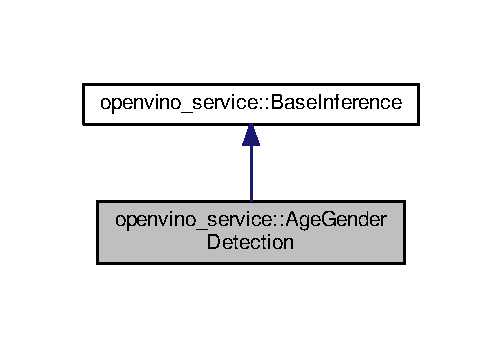
\includegraphics[width=241pt]{classopenvino__service_1_1AgeGenderDetection__inherit__graph}
\end{center}
\end{figure}


Collaboration diagram for openvino\+\_\+service\+:\+:Age\+Gender\+Detection\+:
\nopagebreak
\begin{figure}[H]
\begin{center}
\leavevmode
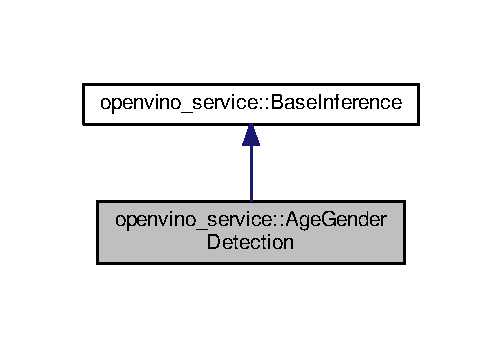
\includegraphics[width=241pt]{classopenvino__service_1_1AgeGenderDetection__coll__graph}
\end{center}
\end{figure}
\subsection*{Public Types}
\begin{DoxyCompactItemize}
\item 
using \hyperlink{classopenvino__service_1_1AgeGenderDetection_aafeb3d01da31d68d5d583c7633e90e0c}{Result} = \hyperlink{structInferenceResult_1_1AgeGenderResult}{Inference\+Result\+::\+Age\+Gender\+Result}
\end{DoxyCompactItemize}
\subsection*{Public Member Functions}
\begin{DoxyCompactItemize}
\item 
\hyperlink{classopenvino__service_1_1AgeGenderDetection_a028a28fcbbdc31168eb6e4f18167ef86}{Age\+Gender\+Detection} ()
\item 
\hyperlink{classopenvino__service_1_1AgeGenderDetection_a91306ff97173c5326b734a09ed49a7fd}{$\sim$\+Age\+Gender\+Detection} () override
\item 
void \hyperlink{classopenvino__service_1_1AgeGenderDetection_a539995501486d88a9e6731762ef5fc8e}{load\+Network} (std\+::shared\+\_\+ptr$<$ \hyperlink{classValidatedAgeGenderNetwork}{Validated\+Age\+Gender\+Network} $>$)
\item 
bool \hyperlink{classopenvino__service_1_1AgeGenderDetection_a2688ef111a3c5f0e96c4a24025519a20}{enqueue} (const cv\+::\+Mat \&frame, const cv\+::\+Rect \&) override
\begin{DoxyCompactList}\small\item\em Enqueue a frame to this class. The frame will be buffered but not infered yet. \end{DoxyCompactList}\item 
bool \hyperlink{classopenvino__service_1_1AgeGenderDetection_ac958ea8415ea449db0613f396d227611}{submit\+Request} () override
\begin{DoxyCompactList}\small\item\em Start inference for all buffered frames. \end{DoxyCompactList}\item 
bool \hyperlink{classopenvino__service_1_1AgeGenderDetection_a3f62deab20335fded7d6b50d5d02c7bb}{fetch\+Results} () override
\begin{DoxyCompactList}\small\item\em This function will fetch the results of the previous inference and stores the results in a result buffer array. All buffered frames will be cleared. \end{DoxyCompactList}\item 
void \hyperlink{classopenvino__service_1_1AgeGenderDetection_a15e5859bb5805fb36696d1e25db91915}{accepts} (std\+::shared\+\_\+ptr$<$ \hyperlink{classBaseOutput}{Base\+Output} $>$ output\+\_\+visitor) override
\begin{DoxyCompactList}\small\item\em Accepts an Output instance for result process. This function is used for visitor pattern. \end{DoxyCompactList}\item 
const \hyperlink{CMakeCache_8txt_a79a3d8790b2588b09777910863574e09}{int} \hyperlink{classopenvino__service_1_1AgeGenderDetection_a61f978e7e856ec5a16867ad0ed1d5180}{get\+Results\+Length} () const override
\begin{DoxyCompactList}\small\item\em Get the length of the buffer result array. \end{DoxyCompactList}\item 
const \hyperlink{structInferenceResult_1_1Result}{Inference\+Result\+::\+Result} \hyperlink{classopenvino__service_1_1AgeGenderDetection_a99ffe0dd90910e5a5df8dc3db24d9dac}{get\+Location\+Result} (\hyperlink{CMakeCache_8txt_a79a3d8790b2588b09777910863574e09}{int} idx) const override
\begin{DoxyCompactList}\small\item\em Get the location of result with respect to the frame generated by the input device. \end{DoxyCompactList}\item 
const std\+::string \hyperlink{classopenvino__service_1_1AgeGenderDetection_a3a0189c3329c9319357cc23c7ee0133f}{get\+Name} () const override
\begin{DoxyCompactList}\small\item\em Get the name of the Inference instance. \end{DoxyCompactList}\end{DoxyCompactItemize}
\subsection*{Additional Inherited Members}


\subsection{Detailed Description}


Definition at line 21 of file age\+\_\+gender\+\_\+recognition.\+h.



\subsection{Member Typedef Documentation}
\index{openvino\+\_\+service\+::\+Age\+Gender\+Detection@{openvino\+\_\+service\+::\+Age\+Gender\+Detection}!Result@{Result}}
\index{Result@{Result}!openvino\+\_\+service\+::\+Age\+Gender\+Detection@{openvino\+\_\+service\+::\+Age\+Gender\+Detection}}
\subsubsection[{\texorpdfstring{Result}{Result}}]{\setlength{\rightskip}{0pt plus 5cm}using {\bf openvino\+\_\+service\+::\+Age\+Gender\+Detection\+::\+Result} =  {\bf Inference\+Result\+::\+Age\+Gender\+Result}}\hypertarget{classopenvino__service_1_1AgeGenderDetection_aafeb3d01da31d68d5d583c7633e90e0c}{}\label{classopenvino__service_1_1AgeGenderDetection_aafeb3d01da31d68d5d583c7633e90e0c}


Definition at line 23 of file age\+\_\+gender\+\_\+recognition.\+h.



\subsection{Constructor \& Destructor Documentation}
\index{openvino\+\_\+service\+::\+Age\+Gender\+Detection@{openvino\+\_\+service\+::\+Age\+Gender\+Detection}!Age\+Gender\+Detection@{Age\+Gender\+Detection}}
\index{Age\+Gender\+Detection@{Age\+Gender\+Detection}!openvino\+\_\+service\+::\+Age\+Gender\+Detection@{openvino\+\_\+service\+::\+Age\+Gender\+Detection}}
\subsubsection[{\texorpdfstring{Age\+Gender\+Detection()}{AgeGenderDetection()}}]{\setlength{\rightskip}{0pt plus 5cm}openvino\+\_\+service\+::\+Age\+Gender\+Detection\+::\+Age\+Gender\+Detection (
\begin{DoxyParamCaption}
{}
\end{DoxyParamCaption}
)\hspace{0.3cm}{\ttfamily [explicit]}}\hypertarget{classopenvino__service_1_1AgeGenderDetection_a028a28fcbbdc31168eb6e4f18167ef86}{}\label{classopenvino__service_1_1AgeGenderDetection_a028a28fcbbdc31168eb6e4f18167ef86}


Definition at line 8 of file age\+\_\+gender\+\_\+recognition.\+cpp.


\begin{DoxyCode}
9     : \hyperlink{classopenvino__service_1_1BaseInference}{openvino\_service::BaseInference}() \{\};
\end{DoxyCode}
\index{openvino\+\_\+service\+::\+Age\+Gender\+Detection@{openvino\+\_\+service\+::\+Age\+Gender\+Detection}!````~Age\+Gender\+Detection@{$\sim$\+Age\+Gender\+Detection}}
\index{````~Age\+Gender\+Detection@{$\sim$\+Age\+Gender\+Detection}!openvino\+\_\+service\+::\+Age\+Gender\+Detection@{openvino\+\_\+service\+::\+Age\+Gender\+Detection}}
\subsubsection[{\texorpdfstring{$\sim$\+Age\+Gender\+Detection() override}{~AgeGenderDetection() override}}]{\setlength{\rightskip}{0pt plus 5cm}openvino\+\_\+service\+::\+Age\+Gender\+Detection\+::$\sim$\+Age\+Gender\+Detection (
\begin{DoxyParamCaption}
{}
\end{DoxyParamCaption}
)\hspace{0.3cm}{\ttfamily [override]}, {\ttfamily [default]}}\hypertarget{classopenvino__service_1_1AgeGenderDetection_a91306ff97173c5326b734a09ed49a7fd}{}\label{classopenvino__service_1_1AgeGenderDetection_a91306ff97173c5326b734a09ed49a7fd}


\subsection{Member Function Documentation}
\index{openvino\+\_\+service\+::\+Age\+Gender\+Detection@{openvino\+\_\+service\+::\+Age\+Gender\+Detection}!accepts@{accepts}}
\index{accepts@{accepts}!openvino\+\_\+service\+::\+Age\+Gender\+Detection@{openvino\+\_\+service\+::\+Age\+Gender\+Detection}}
\subsubsection[{\texorpdfstring{accepts(std\+::shared\+\_\+ptr$<$ Base\+Output $>$ output\+\_\+visitor) override}{accepts(std::shared_ptr< BaseOutput > output_visitor) override}}]{\setlength{\rightskip}{0pt plus 5cm}void openvino\+\_\+service\+::\+Age\+Gender\+Detection\+::accepts (
\begin{DoxyParamCaption}
\item[{std\+::shared\+\_\+ptr$<$ {\bf Base\+Output} $>$}]{output\+\_\+visitor}
\end{DoxyParamCaption}
)\hspace{0.3cm}{\ttfamily [override]}, {\ttfamily [virtual]}}\hypertarget{classopenvino__service_1_1AgeGenderDetection_a15e5859bb5805fb36696d1e25db91915}{}\label{classopenvino__service_1_1AgeGenderDetection_a15e5859bb5805fb36696d1e25db91915}


Accepts an Output instance for result process. This function is used for visitor pattern. 



Implements \hyperlink{classopenvino__service_1_1BaseInference_a910a5b98530670736f525317870c7682}{openvino\+\_\+service\+::\+Base\+Inference}.



Definition at line 52 of file age\+\_\+gender\+\_\+recognition.\+cpp.


\begin{DoxyCode}
53                                               \{
54   \textcolor{keywordflow}{for} (\textcolor{keyword}{auto} &result : results\_) \{
55     output\_visitor->prepareData(result);
56   \}
57 \};
\end{DoxyCode}
\index{openvino\+\_\+service\+::\+Age\+Gender\+Detection@{openvino\+\_\+service\+::\+Age\+Gender\+Detection}!enqueue@{enqueue}}
\index{enqueue@{enqueue}!openvino\+\_\+service\+::\+Age\+Gender\+Detection@{openvino\+\_\+service\+::\+Age\+Gender\+Detection}}
\subsubsection[{\texorpdfstring{enqueue(const cv\+::\+Mat \&frame, const cv\+::\+Rect \&) override}{enqueue(const cv::Mat &frame, const cv::Rect &) override}}]{\setlength{\rightskip}{0pt plus 5cm}bool openvino\+\_\+service\+::\+Age\+Gender\+Detection\+::enqueue (
\begin{DoxyParamCaption}
\item[{const cv\+::\+Mat \&}]{frame, }
\item[{const cv\+::\+Rect \&}]{input\+\_\+frame\+\_\+loc}
\end{DoxyParamCaption}
)\hspace{0.3cm}{\ttfamily [override]}, {\ttfamily [virtual]}}\hypertarget{classopenvino__service_1_1AgeGenderDetection_a2688ef111a3c5f0e96c4a24025519a20}{}\label{classopenvino__service_1_1AgeGenderDetection_a2688ef111a3c5f0e96c4a24025519a20}


Enqueue a frame to this class. The frame will be buffered but not infered yet. 


\begin{DoxyParams}[1]{Parameters}
\mbox{\tt in}  & {\em frame} & The frame to be enqueued. \\
\hline
\mbox{\tt in}  & {\em input\+\_\+frame\+\_\+loc} & The location of the enqueued frame with respect to the frame generated by the input device. \\
\hline
\end{DoxyParams}
\begin{DoxyReturn}{Returns}
whether this operation is successful. 
\end{DoxyReturn}


Implements \hyperlink{classopenvino__service_1_1BaseInference_a907695e3f04fd9ca079cc5a8bab948b1}{openvino\+\_\+service\+::\+Base\+Inference}.



Definition at line 19 of file age\+\_\+gender\+\_\+recognition.\+cpp.


\begin{DoxyCode}
20                                                                                   \{
21   \textcolor{keywordflow}{if} (\hyperlink{classopenvino__service_1_1BaseInference_a130e3cbdc5760a4a42ad5af401398d37}{getEnqueuedNum}() == 0) \{ results\_.clear(); \}
22   \textcolor{keywordtype}{bool} succeed = openvino\_service::BaseInference::enqueue<float>(
23       frame, input\_frame\_loc, 1, \hyperlink{classopenvino__service_1_1AgeGenderDetection_a61f978e7e856ec5a16867ad0ed1d5180}{getResultsLength}(),
24       valid\_network\_->getInputName());
25   \textcolor{keywordflow}{if} (!succeed ) \textcolor{keywordflow}{return} \textcolor{keyword}{false};
26   \hyperlink{classopenvino__service_1_1AgeGenderDetection_aafeb3d01da31d68d5d583c7633e90e0c}{Result} r;
27   r.\hyperlink{structInferenceResult_1_1Result_a20260cebf785b75132140ab517594660}{location} = input\_frame\_loc;
28   results\_.emplace\_back(r);
29   \textcolor{keywordflow}{return} \textcolor{keyword}{true};
30 \}
\end{DoxyCode}
\index{openvino\+\_\+service\+::\+Age\+Gender\+Detection@{openvino\+\_\+service\+::\+Age\+Gender\+Detection}!fetch\+Results@{fetch\+Results}}
\index{fetch\+Results@{fetch\+Results}!openvino\+\_\+service\+::\+Age\+Gender\+Detection@{openvino\+\_\+service\+::\+Age\+Gender\+Detection}}
\subsubsection[{\texorpdfstring{fetch\+Results() override}{fetchResults() override}}]{\setlength{\rightskip}{0pt plus 5cm}bool openvino\+\_\+service\+::\+Age\+Gender\+Detection\+::fetch\+Results (
\begin{DoxyParamCaption}
{}
\end{DoxyParamCaption}
)\hspace{0.3cm}{\ttfamily [override]}, {\ttfamily [virtual]}}\hypertarget{classopenvino__service_1_1AgeGenderDetection_a3f62deab20335fded7d6b50d5d02c7bb}{}\label{classopenvino__service_1_1AgeGenderDetection_a3f62deab20335fded7d6b50d5d02c7bb}


This function will fetch the results of the previous inference and stores the results in a result buffer array. All buffered frames will be cleared. 

\begin{DoxyReturn}{Returns}
whether the Inference object fetches a result this time 
\end{DoxyReturn}


Reimplemented from \hyperlink{classopenvino__service_1_1BaseInference_a9604e193581d6f458634035059342a2c}{openvino\+\_\+service\+::\+Base\+Inference}.



Definition at line 36 of file age\+\_\+gender\+\_\+recognition.\+cpp.


\begin{DoxyCode}
36                                                       \{
37   \textcolor{keywordtype}{bool} can\_fetch = \hyperlink{classopenvino__service_1_1BaseInference_a9604e193581d6f458634035059342a2c}{openvino\_service::BaseInference::fetchResults}
      ();
38   \textcolor{keywordflow}{if} (!can\_fetch) \textcolor{keywordflow}{return} \textcolor{keyword}{false};
39   \textcolor{keyword}{auto} request = \hyperlink{classopenvino__service_1_1BaseInference_a27ef6d92c87dec4480f818a2bcca62a4}{getEngine}()->getRequest();
40   InferenceEngine::Blob::Ptr
41       genderBlob = request->GetBlob(valid\_network\_->getOutputGenderName());
42   InferenceEngine::Blob::Ptr
43       ageBlob = request->GetBlob(valid\_network\_->getOutputAgeName());
44 
45   \textcolor{keywordflow}{for} (\textcolor{keywordtype}{int} i = 0; i < results\_.size(); ++i) \{
46     results\_[i].age = ageBlob->buffer().as<\textcolor{keywordtype}{float} *>()[i] * 100;
47     results\_[i].male\_prob = genderBlob->buffer().as<\textcolor{keywordtype}{float} *>()[i * 2 + 1];
48   \}
49   \textcolor{keywordflow}{return} \textcolor{keyword}{true};
50 \};
\end{DoxyCode}
\index{openvino\+\_\+service\+::\+Age\+Gender\+Detection@{openvino\+\_\+service\+::\+Age\+Gender\+Detection}!get\+Location\+Result@{get\+Location\+Result}}
\index{get\+Location\+Result@{get\+Location\+Result}!openvino\+\_\+service\+::\+Age\+Gender\+Detection@{openvino\+\_\+service\+::\+Age\+Gender\+Detection}}
\subsubsection[{\texorpdfstring{get\+Location\+Result(int idx) const override}{getLocationResult(int idx) const override}}]{\setlength{\rightskip}{0pt plus 5cm}const {\bf Inference\+Result\+::\+Result} openvino\+\_\+service\+::\+Age\+Gender\+Detection\+::get\+Location\+Result (
\begin{DoxyParamCaption}
\item[{{\bf int}}]{idx}
\end{DoxyParamCaption}
) const\hspace{0.3cm}{\ttfamily [override]}, {\ttfamily [virtual]}}\hypertarget{classopenvino__service_1_1AgeGenderDetection_a99ffe0dd90910e5a5df8dc3db24d9dac}{}\label{classopenvino__service_1_1AgeGenderDetection_a99ffe0dd90910e5a5df8dc3db24d9dac}


Get the location of result with respect to the frame generated by the input device. 


\begin{DoxyParams}[1]{Parameters}
\mbox{\tt in}  & {\em idx} & The index of the result. \\
\hline
\end{DoxyParams}


Implements \hyperlink{classopenvino__service_1_1BaseInference_a0e600e89af8796fab69a31732f86c32d}{openvino\+\_\+service\+::\+Base\+Inference}.



Definition at line 64 of file age\+\_\+gender\+\_\+recognition.\+cpp.


\begin{DoxyCode}
64                                                                    \{
65   \textcolor{keywordflow}{return} results\_[idx];
66 \};
\end{DoxyCode}
\index{openvino\+\_\+service\+::\+Age\+Gender\+Detection@{openvino\+\_\+service\+::\+Age\+Gender\+Detection}!get\+Name@{get\+Name}}
\index{get\+Name@{get\+Name}!openvino\+\_\+service\+::\+Age\+Gender\+Detection@{openvino\+\_\+service\+::\+Age\+Gender\+Detection}}
\subsubsection[{\texorpdfstring{get\+Name() const override}{getName() const override}}]{\setlength{\rightskip}{0pt plus 5cm}const std\+::string openvino\+\_\+service\+::\+Age\+Gender\+Detection\+::get\+Name (
\begin{DoxyParamCaption}
{}
\end{DoxyParamCaption}
) const\hspace{0.3cm}{\ttfamily [override]}, {\ttfamily [virtual]}}\hypertarget{classopenvino__service_1_1AgeGenderDetection_a3a0189c3329c9319357cc23c7ee0133f}{}\label{classopenvino__service_1_1AgeGenderDetection_a3a0189c3329c9319357cc23c7ee0133f}


Get the name of the Inference instance. 



Implements \hyperlink{classopenvino__service_1_1BaseInference_add0726f9fc1f0c44288fea3306255bd2}{openvino\+\_\+service\+::\+Base\+Inference}.



Definition at line 68 of file age\+\_\+gender\+\_\+recognition.\+cpp.


\begin{DoxyCode}
68                                                                   \{
69   \textcolor{keywordflow}{return} valid\_network\_->getNetworkName();
70 \}\end{DoxyCode}
\index{openvino\+\_\+service\+::\+Age\+Gender\+Detection@{openvino\+\_\+service\+::\+Age\+Gender\+Detection}!get\+Results\+Length@{get\+Results\+Length}}
\index{get\+Results\+Length@{get\+Results\+Length}!openvino\+\_\+service\+::\+Age\+Gender\+Detection@{openvino\+\_\+service\+::\+Age\+Gender\+Detection}}
\subsubsection[{\texorpdfstring{get\+Results\+Length() const override}{getResultsLength() const override}}]{\setlength{\rightskip}{0pt plus 5cm}const {\bf int} openvino\+\_\+service\+::\+Age\+Gender\+Detection\+::get\+Results\+Length (
\begin{DoxyParamCaption}
{}
\end{DoxyParamCaption}
) const\hspace{0.3cm}{\ttfamily [override]}, {\ttfamily [virtual]}}\hypertarget{classopenvino__service_1_1AgeGenderDetection_a61f978e7e856ec5a16867ad0ed1d5180}{}\label{classopenvino__service_1_1AgeGenderDetection_a61f978e7e856ec5a16867ad0ed1d5180}


Get the length of the buffer result array. 



Implements \hyperlink{classopenvino__service_1_1BaseInference_a6380b6f2baf1e14d5e89922be077d607}{openvino\+\_\+service\+::\+Base\+Inference}.



Definition at line 59 of file age\+\_\+gender\+\_\+recognition.\+cpp.


\begin{DoxyCode}
59                                                                      \{
60   \textcolor{keywordflow}{return} (\textcolor{keywordtype}{int})results\_.size();
61 \};
\end{DoxyCode}
\index{openvino\+\_\+service\+::\+Age\+Gender\+Detection@{openvino\+\_\+service\+::\+Age\+Gender\+Detection}!load\+Network@{load\+Network}}
\index{load\+Network@{load\+Network}!openvino\+\_\+service\+::\+Age\+Gender\+Detection@{openvino\+\_\+service\+::\+Age\+Gender\+Detection}}
\subsubsection[{\texorpdfstring{load\+Network(std\+::shared\+\_\+ptr$<$ Validated\+Age\+Gender\+Network $>$)}{loadNetwork(std::shared_ptr< ValidatedAgeGenderNetwork >)}}]{\setlength{\rightskip}{0pt plus 5cm}void openvino\+\_\+service\+::\+Age\+Gender\+Detection\+::load\+Network (
\begin{DoxyParamCaption}
\item[{std\+::shared\+\_\+ptr$<$ {\bf Validated\+Age\+Gender\+Network} $>$}]{network}
\end{DoxyParamCaption}
)}\hypertarget{classopenvino__service_1_1AgeGenderDetection_a539995501486d88a9e6731762ef5fc8e}{}\label{classopenvino__service_1_1AgeGenderDetection_a539995501486d88a9e6731762ef5fc8e}


Definition at line 13 of file age\+\_\+gender\+\_\+recognition.\+cpp.


\begin{DoxyCode}
14                                                       \{
15   valid\_network\_ = network;
16   \hyperlink{classopenvino__service_1_1BaseInference_a5fde37567347eb98309a530c22335a76}{setMaxBatchSize}(network->getMaxBatchSize());
17 \}
\end{DoxyCode}
\index{openvino\+\_\+service\+::\+Age\+Gender\+Detection@{openvino\+\_\+service\+::\+Age\+Gender\+Detection}!submit\+Request@{submit\+Request}}
\index{submit\+Request@{submit\+Request}!openvino\+\_\+service\+::\+Age\+Gender\+Detection@{openvino\+\_\+service\+::\+Age\+Gender\+Detection}}
\subsubsection[{\texorpdfstring{submit\+Request() override}{submitRequest() override}}]{\setlength{\rightskip}{0pt plus 5cm}bool openvino\+\_\+service\+::\+Age\+Gender\+Detection\+::submit\+Request (
\begin{DoxyParamCaption}
{}
\end{DoxyParamCaption}
)\hspace{0.3cm}{\ttfamily [override]}, {\ttfamily [virtual]}}\hypertarget{classopenvino__service_1_1AgeGenderDetection_ac958ea8415ea449db0613f396d227611}{}\label{classopenvino__service_1_1AgeGenderDetection_ac958ea8415ea449db0613f396d227611}


Start inference for all buffered frames. 

\begin{DoxyReturn}{Returns}
whether this operation is successful. 
\end{DoxyReturn}


Reimplemented from \hyperlink{classopenvino__service_1_1BaseInference_a33b93ef057b95bf7968583e4c2eba0c9}{openvino\+\_\+service\+::\+Base\+Inference}.



Definition at line 32 of file age\+\_\+gender\+\_\+recognition.\+cpp.


\begin{DoxyCode}
32                                                        \{
33   \textcolor{keywordflow}{return} \hyperlink{classopenvino__service_1_1BaseInference_a33b93ef057b95bf7968583e4c2eba0c9}{openvino\_service::BaseInference::submitRequest}();
34 \}
\end{DoxyCode}


The documentation for this class was generated from the following files\+:\begin{DoxyCompactItemize}
\item 
include/openvino\+\_\+service/inferences/\hyperlink{age__gender__recognition_8h}{age\+\_\+gender\+\_\+recognition.\+h}\item 
lib/inferences/\hyperlink{age__gender__recognition_8cpp}{age\+\_\+gender\+\_\+recognition.\+cpp}\end{DoxyCompactItemize}

\hypertarget{structInferenceResult_1_1AgeGenderResult}{}\section{Inference\+Result\+:\+:Age\+Gender\+Result Struct Reference}
\label{structInferenceResult_1_1AgeGenderResult}\index{Inference\+Result\+::\+Age\+Gender\+Result@{Inference\+Result\+::\+Age\+Gender\+Result}}


{\ttfamily \#include $<$data\+\_\+struct.\+h$>$}



Inheritance diagram for Inference\+Result\+:\+:Age\+Gender\+Result\+:
\nopagebreak
\begin{figure}[H]
\begin{center}
\leavevmode
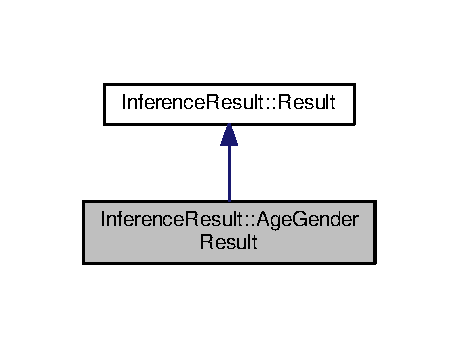
\includegraphics[width=220pt]{structInferenceResult_1_1AgeGenderResult__inherit__graph}
\end{center}
\end{figure}


Collaboration diagram for Inference\+Result\+:\+:Age\+Gender\+Result\+:
\nopagebreak
\begin{figure}[H]
\begin{center}
\leavevmode
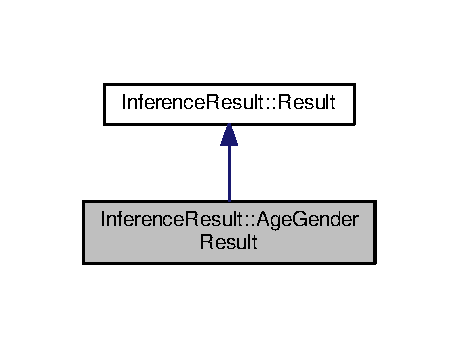
\includegraphics[width=220pt]{structInferenceResult_1_1AgeGenderResult__coll__graph}
\end{center}
\end{figure}
\subsection*{Public Attributes}
\begin{DoxyCompactItemize}
\item 
float \hyperlink{structInferenceResult_1_1AgeGenderResult_a6c4ec413eb257cea2c02cc53a1cfc272}{age} = -\/1
\item 
float \hyperlink{structInferenceResult_1_1AgeGenderResult_a8a17d89e0d1b8bde9eb9d862486493c9}{male\+\_\+prob} = -\/1
\end{DoxyCompactItemize}


\subsection{Detailed Description}


Definition at line 25 of file data\+\_\+struct.\+h.



\subsection{Member Data Documentation}
\index{Inference\+Result\+::\+Age\+Gender\+Result@{Inference\+Result\+::\+Age\+Gender\+Result}!age@{age}}
\index{age@{age}!Inference\+Result\+::\+Age\+Gender\+Result@{Inference\+Result\+::\+Age\+Gender\+Result}}
\subsubsection[{\texorpdfstring{age}{age}}]{\setlength{\rightskip}{0pt plus 5cm}float Inference\+Result\+::\+Age\+Gender\+Result\+::age = -\/1}\hypertarget{structInferenceResult_1_1AgeGenderResult_a6c4ec413eb257cea2c02cc53a1cfc272}{}\label{structInferenceResult_1_1AgeGenderResult_a6c4ec413eb257cea2c02cc53a1cfc272}


Definition at line 26 of file data\+\_\+struct.\+h.

\index{Inference\+Result\+::\+Age\+Gender\+Result@{Inference\+Result\+::\+Age\+Gender\+Result}!male\+\_\+prob@{male\+\_\+prob}}
\index{male\+\_\+prob@{male\+\_\+prob}!Inference\+Result\+::\+Age\+Gender\+Result@{Inference\+Result\+::\+Age\+Gender\+Result}}
\subsubsection[{\texorpdfstring{male\+\_\+prob}{male_prob}}]{\setlength{\rightskip}{0pt plus 5cm}float Inference\+Result\+::\+Age\+Gender\+Result\+::male\+\_\+prob = -\/1}\hypertarget{structInferenceResult_1_1AgeGenderResult_a8a17d89e0d1b8bde9eb9d862486493c9}{}\label{structInferenceResult_1_1AgeGenderResult_a8a17d89e0d1b8bde9eb9d862486493c9}


Definition at line 27 of file data\+\_\+struct.\+h.



The documentation for this struct was generated from the following file\+:\begin{DoxyCompactItemize}
\item 
include/openvino\+\_\+service/\hyperlink{data__struct_8h}{data\+\_\+struct.\+h}\end{DoxyCompactItemize}

\hypertarget{classInferenceEngine_1_1Extensions_1_1Cpu_1_1ArgMaxImpl}{}\section{Inference\+Engine\+:\+:Extensions\+:\+:Cpu\+:\+:Arg\+Max\+Impl Class Reference}
\label{classInferenceEngine_1_1Extensions_1_1Cpu_1_1ArgMaxImpl}\index{Inference\+Engine\+::\+Extensions\+::\+Cpu\+::\+Arg\+Max\+Impl@{Inference\+Engine\+::\+Extensions\+::\+Cpu\+::\+Arg\+Max\+Impl}}


Inheritance diagram for Inference\+Engine\+:\+:Extensions\+:\+:Cpu\+:\+:Arg\+Max\+Impl\+:
\nopagebreak
\begin{figure}[H]
\begin{center}
\leavevmode
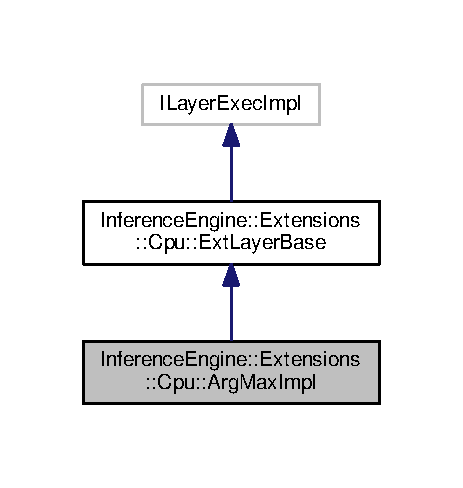
\includegraphics[width=222pt]{classInferenceEngine_1_1Extensions_1_1Cpu_1_1ArgMaxImpl__inherit__graph}
\end{center}
\end{figure}


Collaboration diagram for Inference\+Engine\+:\+:Extensions\+:\+:Cpu\+:\+:Arg\+Max\+Impl\+:
\nopagebreak
\begin{figure}[H]
\begin{center}
\leavevmode
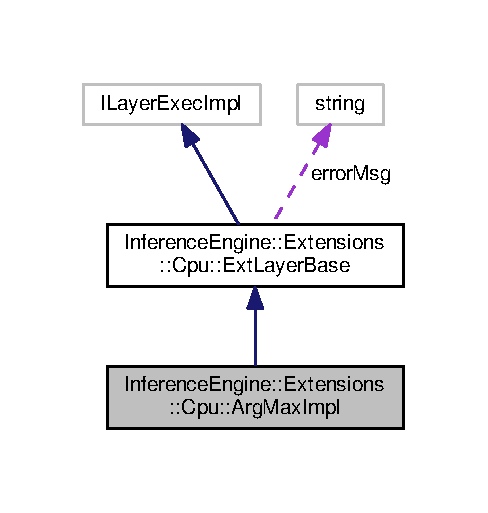
\includegraphics[width=234pt]{classInferenceEngine_1_1Extensions_1_1Cpu_1_1ArgMaxImpl__coll__graph}
\end{center}
\end{figure}
\subsection*{Public Member Functions}
\begin{DoxyCompactItemize}
\item 
\hyperlink{classInferenceEngine_1_1Extensions_1_1Cpu_1_1ArgMaxImpl_a9344fd147a948eab35731fbbb69d2e99}{Arg\+Max\+Impl} (const C\+N\+N\+Layer $\ast$layer)
\item 
Status\+Code \hyperlink{classInferenceEngine_1_1Extensions_1_1Cpu_1_1ArgMaxImpl_a4acb850c8f11dd20040cb02ffe6222da}{execute} (std\+::vector$<$ Blob\+::\+Ptr $>$ \&inputs, std\+::vector$<$ Blob\+::\+Ptr $>$ \&outputs, Response\+Desc $\ast$resp) noexceptoverride
\end{DoxyCompactItemize}
\subsection*{Additional Inherited Members}


\subsection{Detailed Description}


Definition at line 31 of file ext\+\_\+argmax.\+cpp.



\subsection{Constructor \& Destructor Documentation}
\index{Inference\+Engine\+::\+Extensions\+::\+Cpu\+::\+Arg\+Max\+Impl@{Inference\+Engine\+::\+Extensions\+::\+Cpu\+::\+Arg\+Max\+Impl}!Arg\+Max\+Impl@{Arg\+Max\+Impl}}
\index{Arg\+Max\+Impl@{Arg\+Max\+Impl}!Inference\+Engine\+::\+Extensions\+::\+Cpu\+::\+Arg\+Max\+Impl@{Inference\+Engine\+::\+Extensions\+::\+Cpu\+::\+Arg\+Max\+Impl}}
\subsubsection[{\texorpdfstring{Arg\+Max\+Impl(const C\+N\+N\+Layer $\ast$layer)}{ArgMaxImpl(const CNNLayer *layer)}}]{\setlength{\rightskip}{0pt plus 5cm}Inference\+Engine\+::\+Extensions\+::\+Cpu\+::\+Arg\+Max\+Impl\+::\+Arg\+Max\+Impl (
\begin{DoxyParamCaption}
\item[{const C\+N\+N\+Layer $\ast$}]{layer}
\end{DoxyParamCaption}
)\hspace{0.3cm}{\ttfamily [inline]}, {\ttfamily [explicit]}}\hypertarget{classInferenceEngine_1_1Extensions_1_1Cpu_1_1ArgMaxImpl_a9344fd147a948eab35731fbbb69d2e99}{}\label{classInferenceEngine_1_1Extensions_1_1Cpu_1_1ArgMaxImpl_a9344fd147a948eab35731fbbb69d2e99}


Definition at line 33 of file ext\+\_\+argmax.\+cpp.


\begin{DoxyCode}
33                                               : \hyperlink{classInferenceEngine_1_1Extensions_1_1Cpu_1_1ExtLayerBase_affff0e8263ca26852ccf71d299d7b06a}{ExtLayerBase}(layer) \{
34         \textcolor{keywordflow}{try} \{
35             \textcolor{keywordflow}{if} (\hyperlink{classInferenceEngine_1_1Extensions_1_1Cpu_1_1ExtLayerBase_a1074cdccacb9e9ca6eec01bbc2f7ca4a}{cnnLayer}.insData.size() != 1 || \hyperlink{classInferenceEngine_1_1Extensions_1_1Cpu_1_1ExtLayerBase_a1074cdccacb9e9ca6eec01bbc2f7ca4a}{cnnLayer}.outData.empty())
36                 THROW\_IE\_EXCEPTION << \textcolor{stringliteral}{"Incorrect number of input/output edges!"};
37 
38             out\_max\_val\_ = \textcolor{keyword}{static\_cast<}\textcolor{keywordtype}{bool}\textcolor{keyword}{>}(\hyperlink{classInferenceEngine_1_1Extensions_1_1Cpu_1_1ExtLayerBase_a1074cdccacb9e9ca6eec01bbc2f7ca4a}{cnnLayer}.GetParamAsInt(\textcolor{stringliteral}{"out\_max\_val"}));
39             top\_k\_       = \hyperlink{classInferenceEngine_1_1Extensions_1_1Cpu_1_1ExtLayerBase_a1074cdccacb9e9ca6eec01bbc2f7ca4a}{cnnLayer}.GetParamAsInt(\textcolor{stringliteral}{"top\_k"});
40 
41             has\_axis\_ = (\hyperlink{classInferenceEngine_1_1Extensions_1_1Cpu_1_1ExtLayerBase_a1074cdccacb9e9ca6eec01bbc2f7ca4a}{cnnLayer}.params.find(\textcolor{stringliteral}{"axis"}) != \hyperlink{classInferenceEngine_1_1Extensions_1_1Cpu_1_1ExtLayerBase_a1074cdccacb9e9ca6eec01bbc2f7ca4a}{cnnLayer}.params.end());
42             axis\_index\_ = has\_axis\_ ?
43                                 std::stoi(\hyperlink{classInferenceEngine_1_1Extensions_1_1Cpu_1_1ExtLayerBase_a1074cdccacb9e9ca6eec01bbc2f7ca4a}{cnnLayer}.params[\textcolor{stringliteral}{"axis"}]) :0;
44 
45             \hyperlink{classInferenceEngine_1_1Extensions_1_1Cpu_1_1ExtLayerBase_a0ac7a6632e95b9500d5246b05b4b0bfa}{addConfig}(\{DataConfigurator(\hyperlink{classInferenceEngine_1_1Extensions_1_1Cpu_1_1ExtLayerBase_a1258a8d209e0249e0b1717618352ddfba446687ea2db1ada75be5ed053be77f59}{ConfLayout::PLN})\}, \{DataConfigurator(
      \hyperlink{classInferenceEngine_1_1Extensions_1_1Cpu_1_1ExtLayerBase_a1258a8d209e0249e0b1717618352ddfba446687ea2db1ada75be5ed053be77f59}{ConfLayout::PLN})\});
46         \} \textcolor{keywordflow}{catch} (InferenceEngine::details::InferenceEngineException &ex) \{
47             \hyperlink{classInferenceEngine_1_1Extensions_1_1Cpu_1_1ExtLayerBase_abc78e9b5a79fa339ffd831a5318f71f7}{errorMsg} = ex.what();
48         \}
49     \}
\end{DoxyCode}


\subsection{Member Function Documentation}
\index{Inference\+Engine\+::\+Extensions\+::\+Cpu\+::\+Arg\+Max\+Impl@{Inference\+Engine\+::\+Extensions\+::\+Cpu\+::\+Arg\+Max\+Impl}!execute@{execute}}
\index{execute@{execute}!Inference\+Engine\+::\+Extensions\+::\+Cpu\+::\+Arg\+Max\+Impl@{Inference\+Engine\+::\+Extensions\+::\+Cpu\+::\+Arg\+Max\+Impl}}
\subsubsection[{\texorpdfstring{execute(std\+::vector$<$ Blob\+::\+Ptr $>$ \&inputs, std\+::vector$<$ Blob\+::\+Ptr $>$ \&outputs, Response\+Desc $\ast$resp) noexceptoverride}{execute(std::vector< Blob::Ptr > &inputs, std::vector< Blob::Ptr > &outputs, ResponseDesc *resp) noexceptoverride}}]{\setlength{\rightskip}{0pt plus 5cm}Status\+Code Inference\+Engine\+::\+Extensions\+::\+Cpu\+::\+Arg\+Max\+Impl\+::execute (
\begin{DoxyParamCaption}
\item[{std\+::vector$<$ Blob\+::\+Ptr $>$ \&}]{inputs, }
\item[{std\+::vector$<$ Blob\+::\+Ptr $>$ \&}]{outputs, }
\item[{Response\+Desc $\ast$}]{resp}
\end{DoxyParamCaption}
)\hspace{0.3cm}{\ttfamily [inline]}, {\ttfamily [override]}, {\ttfamily [noexcept]}}\hypertarget{classInferenceEngine_1_1Extensions_1_1Cpu_1_1ArgMaxImpl_a4acb850c8f11dd20040cb02ffe6222da}{}\label{classInferenceEngine_1_1Extensions_1_1Cpu_1_1ArgMaxImpl_a4acb850c8f11dd20040cb02ffe6222da}


Definition at line 51 of file ext\+\_\+argmax.\+cpp.


\begin{DoxyCode}
52                                                              \{
53         SizeVector in\_dims = inputs[0]->getTensorDesc().getDims();
54         SizeVector out\_dims = outputs[0]->getTensorDesc().getDims();
55 
56         \textcolor{keywordtype}{int} dim, axis\_dist;
57         \textcolor{keywordflow}{if} (has\_axis\_) \{
58             \textcolor{keywordtype}{int} axis\_ = (axis\_index\_ < 0) ? axis\_index\_ + static\_cast<int>(in\_dims.size()) : axis\_index\_;
59             dim = \textcolor{keyword}{static\_cast<}\textcolor{keywordtype}{int}\textcolor{keyword}{>}(inputs[0]->getTensorDesc().getDims()[axis\_]);
60             axis\_dist = count(inputs[0]->getTensorDesc().getDims(), axis\_) / dim;
61         \} \textcolor{keywordflow}{else} \{
62             dim = count(inputs[0]->getTensorDesc().getDims(), 1);
63             axis\_dist = 1;
64         \}
65 
66         \textcolor{keywordtype}{float}* src\_data = inputs[0]->buffer();
67         \textcolor{keywordtype}{float}* dst\_data = outputs[0]->buffer();
68 
69         \textcolor{keywordtype}{int} num = count(in\_dims) / dim;
70         std::vector<std::pair<float, int> > src\_vector(dim);
71 
72         \textcolor{keywordflow}{for} (\textcolor{keywordtype}{int} i = 0; i < num; ++i) \{
73             \textcolor{keywordflow}{for} (\textcolor{keywordtype}{int} j = 0; j < dim; ++j) \{
74                 src\_vector[j] = std::make\_pair(
75                         src\_data[(i / axis\_dist * dim + j) * axis\_dist + i % axis\_dist], j);
76             \}
77 
78             std::partial\_sort(src\_vector.begin(), src\_vector.begin() + top\_k\_,
79                               src\_vector.end(), std::greater<std::pair<float, int> >());
80 
81             \textcolor{keywordflow}{for} (\textcolor{keywordtype}{int} j = 0; j < top\_k\_; ++j) \{
82                 \textcolor{keywordflow}{if} (out\_max\_val\_) \{
83                     \textcolor{keywordflow}{if} (has\_axis\_) \{
84                         \textcolor{comment}{// Produces max\_val per axis}
85                         dst\_data[(i / axis\_dist * top\_k\_ + j) * axis\_dist + i % axis\_dist] = src\_vector[j].
      first;
86                     \} \textcolor{keywordflow}{else} \{
87                         \textcolor{comment}{// Produces max\_ind and max\_val}
88                         dst\_data[2 * i * top\_k\_ + j] = src\_vector[j].second;
89                         dst\_data[2 * i * top\_k\_ + top\_k\_ + j] = src\_vector[j].first;
90                     \}
91                 \} \textcolor{keywordflow}{else} \{
92                     \textcolor{comment}{// Produces max\_ind per axis}
93                     dst\_data[(i / axis\_dist * top\_k\_ + j) * axis\_dist + i % axis\_dist] = src\_vector[j].
      second;
94                 \}
95             \}
96         \}
97 
98         \textcolor{keywordflow}{return} OK;
99     \}
\end{DoxyCode}


The documentation for this class was generated from the following file\+:\begin{DoxyCompactItemize}
\item 
thirdparty/extension/\hyperlink{ext__argmax_8cpp}{ext\+\_\+argmax.\+cpp}\end{DoxyCompactItemize}

\hypertarget{structAveragePrecisionCalculator}{}\section{Average\+Precision\+Calculator Struct Reference}
\label{structAveragePrecisionCalculator}\index{Average\+Precision\+Calculator@{Average\+Precision\+Calculator}}


{\ttfamily \#include $<$common.\+hpp$>$}

\subsection*{Public Member Functions}
\begin{DoxyCompactItemize}
\item 
\hyperlink{structAveragePrecisionCalculator_ab552a6087e585fcdf5555c6fd05eb98c}{Average\+Precision\+Calculator} (double threshold)
\item 
void \hyperlink{structAveragePrecisionCalculator_a70ca18f1cff4c437ce60fffbb0559347}{consume\+Image} (const \hyperlink{classImageDescription}{Image\+Description} \&detected\+Objects, const \hyperlink{classImageDescription}{Image\+Description} \&desired\+Objects)
\item 
std\+::map$<$ \hyperlink{CMakeCache_8txt_a79a3d8790b2588b09777910863574e09}{int}, double $>$ \hyperlink{structAveragePrecisionCalculator_aebdc3e49c0ada0dc2168bff7ebc6df95}{calculate\+Average\+Precision\+Per\+Class} () const 
\end{DoxyCompactItemize}


\subsection{Detailed Description}


Definition at line 828 of file common.\+hpp.



\subsection{Constructor \& Destructor Documentation}
\index{Average\+Precision\+Calculator@{Average\+Precision\+Calculator}!Average\+Precision\+Calculator@{Average\+Precision\+Calculator}}
\index{Average\+Precision\+Calculator@{Average\+Precision\+Calculator}!Average\+Precision\+Calculator@{Average\+Precision\+Calculator}}
\subsubsection[{\texorpdfstring{Average\+Precision\+Calculator(double threshold)}{AveragePrecisionCalculator(double threshold)}}]{\setlength{\rightskip}{0pt plus 5cm}Average\+Precision\+Calculator\+::\+Average\+Precision\+Calculator (
\begin{DoxyParamCaption}
\item[{double}]{threshold}
\end{DoxyParamCaption}
)\hspace{0.3cm}{\ttfamily [inline]}}\hypertarget{structAveragePrecisionCalculator_ab552a6087e585fcdf5555c6fd05eb98c}{}\label{structAveragePrecisionCalculator_ab552a6087e585fcdf5555c6fd05eb98c}


Definition at line 852 of file common.\+hpp.


\begin{DoxyCode}
852 : threshold(threshold) \{ \}
\end{DoxyCode}


\subsection{Member Function Documentation}
\index{Average\+Precision\+Calculator@{Average\+Precision\+Calculator}!calculate\+Average\+Precision\+Per\+Class@{calculate\+Average\+Precision\+Per\+Class}}
\index{calculate\+Average\+Precision\+Per\+Class@{calculate\+Average\+Precision\+Per\+Class}!Average\+Precision\+Calculator@{Average\+Precision\+Calculator}}
\subsubsection[{\texorpdfstring{calculate\+Average\+Precision\+Per\+Class() const }{calculateAveragePrecisionPerClass() const }}]{\setlength{\rightskip}{0pt plus 5cm}std\+::map$<${\bf int}, double$>$ Average\+Precision\+Calculator\+::calculate\+Average\+Precision\+Per\+Class (
\begin{DoxyParamCaption}
{}
\end{DoxyParamCaption}
) const\hspace{0.3cm}{\ttfamily [inline]}}\hypertarget{structAveragePrecisionCalculator_aebdc3e49c0ada0dc2168bff7ebc6df95}{}\label{structAveragePrecisionCalculator_aebdc3e49c0ada0dc2168bff7ebc6df95}
Precision-\/to-\/\+TP curve per class (a variation of precision-\/to-\/recall curve without dividing into N)

Definition at line 908 of file common.\+hpp.


\begin{DoxyCode}
908                                                                   \{
912         std::map<int, std::map<int, double>> precisionToTP;
913 
914 
915         std::map<int, double> res;
916 
917         \textcolor{keywordtype}{double} AP = 0;
918         \textcolor{keywordtype}{double} q = 0;
919         \textcolor{keywordflow}{for} (\textcolor{keyword}{auto} m : matches) \{
920             \textcolor{comment}{// Sorting}
921             std::sort(m.second.begin(), m.second.end(), SortPairDescend);
922 
923             \textcolor{keywordtype}{int} clazz = m.first;
924             \textcolor{keywordtype}{int} TP = 0, FP = 0;
925 
926             std::vector<double> prec;
927             std::vector<double> rec;
928 
929             \textcolor{keywordflow}{for} (\textcolor{keyword}{auto} mm : m.second) \{
930                 \textcolor{comment}{// Here we are descending in a probability value}
931                 MatchKind mk = mm.second;
932                 \textcolor{keywordflow}{if} (mk == TruePositive) TP++;
933                 \textcolor{keywordflow}{else} \textcolor{keywordflow}{if} (mk == FalsePositive) FP++;
934 
935                 \textcolor{keywordtype}{double} precision = \textcolor{keyword}{static\_cast<}\textcolor{keywordtype}{double}\textcolor{keyword}{>}(TP) / (TP + FP);
936                 \textcolor{keywordtype}{double} recall = 0;
937                 \textcolor{keywordflow}{if} (N.find(clazz) != N.end()) \{
938                     recall = \textcolor{keyword}{static\_cast<}\textcolor{keywordtype}{double}\textcolor{keyword}{>}(TP) / N.at(clazz);
939                 \}
940 
941                 prec.push\_back(precision);
942                 rec.push\_back(recall);
943             \}
944 
945             \textcolor{keywordtype}{int} num = rec.size();
946 
947             \textcolor{comment}{// 11point from Caffe}
948             \textcolor{keywordtype}{double} ap = 0;
949             std::vector<float> max\_precs(11, 0.);
950             \textcolor{keywordtype}{int} start\_idx = num - 1;
951             \textcolor{keywordflow}{for} (\textcolor{keywordtype}{int} j = 10; j >= 0; --j) \{
952                 \textcolor{keywordflow}{for} (\textcolor{keywordtype}{int} i = start\_idx; i >= 0; --i) \{
953                     \textcolor{keywordflow}{if} (rec[i] < j / 10.) \{
954                         start\_idx = i;
955                         \textcolor{keywordflow}{if} (j > 0) \{
956                             max\_precs[j-1] = max\_precs[j];
957                         \}
958                         \textcolor{keywordflow}{break};
959                     \} \textcolor{keywordflow}{else} \{
960                         \textcolor{keywordflow}{if} (max\_precs[j] < prec[i]) \{
961                             max\_precs[j] = prec[i];
962                         \}
963                     \}
964                 \}
965             \}
966             \textcolor{keywordflow}{for} (\textcolor{keywordtype}{int} j = 10; j >= 0; --j) \{
967                 ap += max\_precs[j] / 11;
968             \}
969             res[clazz] = ap;
970         \}
971 
972         \textcolor{keywordflow}{return} res;
973     \}
\end{DoxyCode}
\index{Average\+Precision\+Calculator@{Average\+Precision\+Calculator}!consume\+Image@{consume\+Image}}
\index{consume\+Image@{consume\+Image}!Average\+Precision\+Calculator@{Average\+Precision\+Calculator}}
\subsubsection[{\texorpdfstring{consume\+Image(const Image\+Description \&detected\+Objects, const Image\+Description \&desired\+Objects)}{consumeImage(const ImageDescription &detectedObjects, const ImageDescription &desiredObjects)}}]{\setlength{\rightskip}{0pt plus 5cm}void Average\+Precision\+Calculator\+::consume\+Image (
\begin{DoxyParamCaption}
\item[{const {\bf Image\+Description} \&}]{detected\+Objects, }
\item[{const {\bf Image\+Description} \&}]{desired\+Objects}
\end{DoxyParamCaption}
)\hspace{0.3cm}{\ttfamily [inline]}}\hypertarget{structAveragePrecisionCalculator_a70ca18f1cff4c437ce60fffbb0559347}{}\label{structAveragePrecisionCalculator_a70ca18f1cff4c437ce60fffbb0559347}


Definition at line 857 of file common.\+hpp.


\begin{DoxyCode}
857                                                                                                        \{
858             \textcolor{comment}{// Collecting IoU values}
859         \textcolor{keywordtype}{int} tp = 0, fp = 0;
860 
861         std::vector<bool> visited(desiredObjects.\hyperlink{classImageDescription_aa814580e2dd58fc3442ddd3549e6d81d}{alist}.size(), \textcolor{keyword}{false});
862         std::vector<DetectedObject> bboxes\{ std::begin(detectedObjects.\hyperlink{classImageDescription_aa814580e2dd58fc3442ddd3549e6d81d}{alist}), std::end(
      detectedObjects.\hyperlink{classImageDescription_aa814580e2dd58fc3442ddd3549e6d81d}{alist}) \};
863         std::sort(bboxes.begin(), bboxes.end(), SortBBoxDescend);
864 
865 
866         \textcolor{keywordflow}{for} (\textcolor{keyword}{auto}&& detObj : bboxes) \{
867                 \textcolor{comment}{// Searching for the best match to this detection}
868 
869             \textcolor{comment}{// Searching for desired object}
870             \textcolor{keywordtype}{float} overlap\_max = -1;
871             \textcolor{keywordtype}{int} jmax = -1;
872             \textcolor{keyword}{auto} desmax = desiredObjects.\hyperlink{classImageDescription_aa814580e2dd58fc3442ddd3549e6d81d}{alist}.end();
873 
874             \textcolor{keywordtype}{int} j = 0;
875             \textcolor{keywordflow}{for} (\textcolor{keyword}{auto} desObj = desiredObjects.\hyperlink{classImageDescription_aa814580e2dd58fc3442ddd3549e6d81d}{alist}.begin(); desObj != desiredObjects.
      \hyperlink{classImageDescription_aa814580e2dd58fc3442ddd3549e6d81d}{alist}.end(); desObj++, j++) \{
876                 \textcolor{keywordtype}{double} iou = \hyperlink{classDetectedObject_abc68e001862990d52703deff97fe0db6}{DetectedObject::ioU}(detObj, *desObj);
877                 \textcolor{keywordflow}{if} (iou > overlap\_max) \{
878                     overlap\_max = iou;
879                     jmax = j;
880                     desmax = desObj;
881                 \}
882             \}
883 
884             MatchKind mk;
885             \textcolor{keywordflow}{if} (overlap\_max >= threshold) \{
886                 \textcolor{keywordflow}{if} (!desmax->difficult) \{
887                     \textcolor{keywordflow}{if} (!visited[jmax]) \{
888                         mk = TruePositive;
889                         visited[jmax] = \textcolor{keyword}{true};
890                     \} \textcolor{keywordflow}{else} \{
891                         mk = FalsePositive;
892                     \}
893                     matches[detObj.objectType].push\_back(std::make\_pair(detObj.prob, mk));
894                 \}
895             \} \textcolor{keywordflow}{else} \{
896                 mk = FalsePositive;
897                 matches[detObj.objectType].push\_back(std::make\_pair(detObj.prob, mk));
898             \}
899         \}
900 
901         \textcolor{keywordflow}{for} (\textcolor{keyword}{auto} desObj = desiredObjects.\hyperlink{classImageDescription_aa814580e2dd58fc3442ddd3549e6d81d}{alist}.begin(); desObj != desiredObjects.
      \hyperlink{classImageDescription_aa814580e2dd58fc3442ddd3549e6d81d}{alist}.end(); desObj++) \{
902             \textcolor{keywordflow}{if} (!desObj->difficult) \{
903                 N[desObj->objectType]++;
904                 \}
905             \}
906         \}
\end{DoxyCode}


The documentation for this struct was generated from the following file\+:\begin{DoxyCompactItemize}
\item 
include/openvino\+\_\+service/\hyperlink{common_8hpp}{common.\+hpp}\end{DoxyCompactItemize}

\hypertarget{classopenvino__service_1_1BaseInference}{}\section{openvino\+\_\+service\+:\+:Base\+Inference Class Reference}
\label{classopenvino__service_1_1BaseInference}\index{openvino\+\_\+service\+::\+Base\+Inference@{openvino\+\_\+service\+::\+Base\+Inference}}


base class for network inference.  




{\ttfamily \#include $<$base\+\_\+inference.\+h$>$}



Inheritance diagram for openvino\+\_\+service\+:\+:Base\+Inference\+:
\nopagebreak
\begin{figure}[H]
\begin{center}
\leavevmode
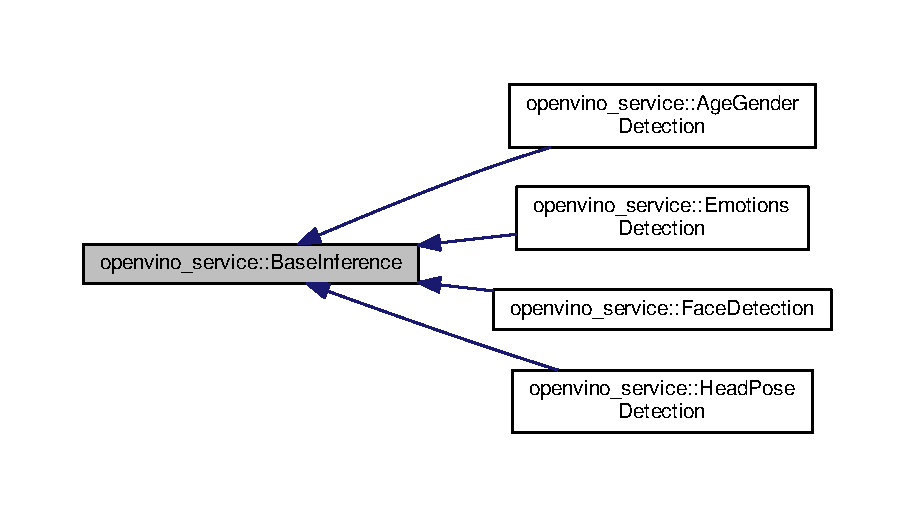
\includegraphics[width=350pt]{classopenvino__service_1_1BaseInference__inherit__graph}
\end{center}
\end{figure}
\subsection*{Public Member Functions}
\begin{DoxyCompactItemize}
\item 
\hyperlink{classopenvino__service_1_1BaseInference_ac44efffac6ad744cac77866a1b4e6044}{Base\+Inference} ()
\item 
virtual \hyperlink{classopenvino__service_1_1BaseInference_a6d93394f51aacb7657359f7d7995b351}{$\sim$\+Base\+Inference} ()
\item 
void \hyperlink{classopenvino__service_1_1BaseInference_a90c8aa5a53236276fe06df8116bcf724}{load\+Engine} (std\+::shared\+\_\+ptr$<$ \hyperlink{classNetworkEngine}{Network\+Engine} $>$ engine)
\begin{DoxyCompactList}\small\item\em load the Engine instance that contains the request for running netwrok on target calculation device. \end{DoxyCompactList}\item 
const std\+::shared\+\_\+ptr$<$ \hyperlink{classNetworkEngine}{Network\+Engine} $>$ \hyperlink{classopenvino__service_1_1BaseInference_a27ef6d92c87dec4480f818a2bcca62a4}{get\+Engine} () const 
\begin{DoxyCompactList}\small\item\em Get the loaded Engine instance. \end{DoxyCompactList}\item 
const \hyperlink{CMakeCache_8txt_a79a3d8790b2588b09777910863574e09}{int} \hyperlink{classopenvino__service_1_1BaseInference_a130e3cbdc5760a4a42ad5af401398d37}{get\+Enqueued\+Num} () const 
\begin{DoxyCompactList}\small\item\em Get the number of enqueued frames to be infered. \end{DoxyCompactList}\item 
virtual bool \hyperlink{classopenvino__service_1_1BaseInference_a907695e3f04fd9ca079cc5a8bab948b1}{enqueue} (const cv\+::\+Mat \&frame, const cv\+::\+Rect \&input\+\_\+frame\+\_\+loc)=0
\begin{DoxyCompactList}\small\item\em Enqueue a frame to this class. The frame will be buffered but not infered yet. \end{DoxyCompactList}\item 
virtual bool \hyperlink{classopenvino__service_1_1BaseInference_a33b93ef057b95bf7968583e4c2eba0c9}{submit\+Request} ()
\begin{DoxyCompactList}\small\item\em Start inference for all buffered frames. \end{DoxyCompactList}\item 
virtual bool \hyperlink{classopenvino__service_1_1BaseInference_a9604e193581d6f458634035059342a2c}{fetch\+Results} ()
\begin{DoxyCompactList}\small\item\em This function will fetch the results of the previous inference and stores the results in a result buffer array. All buffered frames will be cleared. \end{DoxyCompactList}\item 
virtual void \hyperlink{classopenvino__service_1_1BaseInference_a910a5b98530670736f525317870c7682}{accepts} (std\+::shared\+\_\+ptr$<$ \hyperlink{classBaseOutput}{Base\+Output} $>$ output\+\_\+visitor)=0
\begin{DoxyCompactList}\small\item\em Accepts an Output instance for result process. This function is used for visitor pattern. \end{DoxyCompactList}\item 
virtual const \hyperlink{CMakeCache_8txt_a79a3d8790b2588b09777910863574e09}{int} \hyperlink{classopenvino__service_1_1BaseInference_a6380b6f2baf1e14d5e89922be077d607}{get\+Results\+Length} () const =0
\begin{DoxyCompactList}\small\item\em Get the length of the buffer result array. \end{DoxyCompactList}\item 
virtual const \hyperlink{structInferenceResult_1_1Result}{Inference\+Result\+::\+Result} \hyperlink{classopenvino__service_1_1BaseInference_a0e600e89af8796fab69a31732f86c32d}{get\+Location\+Result} (\hyperlink{CMakeCache_8txt_a79a3d8790b2588b09777910863574e09}{int} idx) const =0
\begin{DoxyCompactList}\small\item\em Get the location of result with respect to the frame generated by the input device. \end{DoxyCompactList}\item 
virtual const std\+::string \hyperlink{classopenvino__service_1_1BaseInference_add0726f9fc1f0c44288fea3306255bd2}{get\+Name} () const =0
\begin{DoxyCompactList}\small\item\em Get the name of the Inference instance. \end{DoxyCompactList}\end{DoxyCompactItemize}
\subsection*{Protected Member Functions}
\begin{DoxyCompactItemize}
\item 
{\footnotesize template$<$typename T $>$ }\\bool \hyperlink{classopenvino__service_1_1BaseInference_a11acca6926bf1ed6a23f53ca76673715}{enqueue} (const cv\+::\+Mat \&frame, const cv\+::\+Rect \&, float scale\+\_\+factor, \hyperlink{CMakeCache_8txt_a79a3d8790b2588b09777910863574e09}{int} batch\+\_\+index, const std\+::string \&input\+\_\+name)
\begin{DoxyCompactList}\small\item\em Enqueue the fram into the input blob of the target calculation device. Check Open\+V\+I\+NO document for detailed information. \end{DoxyCompactList}\item 
void \hyperlink{classopenvino__service_1_1BaseInference_a5fde37567347eb98309a530c22335a76}{set\+Max\+Batch\+Size} (\hyperlink{CMakeCache_8txt_a79a3d8790b2588b09777910863574e09}{int} max\+\_\+batch\+\_\+size)
\begin{DoxyCompactList}\small\item\em Set the max batch size for one inference. \end{DoxyCompactList}\end{DoxyCompactItemize}


\subsection{Detailed Description}
base class for network inference. 

Definition at line 53 of file base\+\_\+inference.\+h.



\subsection{Constructor \& Destructor Documentation}
\index{openvino\+\_\+service\+::\+Base\+Inference@{openvino\+\_\+service\+::\+Base\+Inference}!Base\+Inference@{Base\+Inference}}
\index{Base\+Inference@{Base\+Inference}!openvino\+\_\+service\+::\+Base\+Inference@{openvino\+\_\+service\+::\+Base\+Inference}}
\subsubsection[{\texorpdfstring{Base\+Inference()}{BaseInference()}}]{\setlength{\rightskip}{0pt plus 5cm}openvino\+\_\+service\+::\+Base\+Inference\+::\+Base\+Inference (
\begin{DoxyParamCaption}
{}
\end{DoxyParamCaption}
)\hspace{0.3cm}{\ttfamily [explicit]}, {\ttfamily [default]}}\hypertarget{classopenvino__service_1_1BaseInference_ac44efffac6ad744cac77866a1b4e6044}{}\label{classopenvino__service_1_1BaseInference_ac44efffac6ad744cac77866a1b4e6044}
\index{openvino\+\_\+service\+::\+Base\+Inference@{openvino\+\_\+service\+::\+Base\+Inference}!````~Base\+Inference@{$\sim$\+Base\+Inference}}
\index{````~Base\+Inference@{$\sim$\+Base\+Inference}!openvino\+\_\+service\+::\+Base\+Inference@{openvino\+\_\+service\+::\+Base\+Inference}}
\subsubsection[{\texorpdfstring{$\sim$\+Base\+Inference()}{~BaseInference()}}]{\setlength{\rightskip}{0pt plus 5cm}openvino\+\_\+service\+::\+Base\+Inference\+::$\sim$\+Base\+Inference (
\begin{DoxyParamCaption}
{}
\end{DoxyParamCaption}
)\hspace{0.3cm}{\ttfamily [virtual]}, {\ttfamily [default]}}\hypertarget{classopenvino__service_1_1BaseInference_a6d93394f51aacb7657359f7d7995b351}{}\label{classopenvino__service_1_1BaseInference_a6d93394f51aacb7657359f7d7995b351}


\subsection{Member Function Documentation}
\index{openvino\+\_\+service\+::\+Base\+Inference@{openvino\+\_\+service\+::\+Base\+Inference}!accepts@{accepts}}
\index{accepts@{accepts}!openvino\+\_\+service\+::\+Base\+Inference@{openvino\+\_\+service\+::\+Base\+Inference}}
\subsubsection[{\texorpdfstring{accepts(std\+::shared\+\_\+ptr$<$ Base\+Output $>$ output\+\_\+visitor)=0}{accepts(std::shared_ptr< BaseOutput > output_visitor)=0}}]{\setlength{\rightskip}{0pt plus 5cm}virtual void openvino\+\_\+service\+::\+Base\+Inference\+::accepts (
\begin{DoxyParamCaption}
\item[{std\+::shared\+\_\+ptr$<$ {\bf Base\+Output} $>$}]{output\+\_\+visitor}
\end{DoxyParamCaption}
)\hspace{0.3cm}{\ttfamily [pure virtual]}}\hypertarget{classopenvino__service_1_1BaseInference_a910a5b98530670736f525317870c7682}{}\label{classopenvino__service_1_1BaseInference_a910a5b98530670736f525317870c7682}


Accepts an Output instance for result process. This function is used for visitor pattern. 



Implemented in \hyperlink{classopenvino__service_1_1AgeGenderDetection_a15e5859bb5805fb36696d1e25db91915}{openvino\+\_\+service\+::\+Age\+Gender\+Detection}, \hyperlink{classopenvino__service_1_1HeadPoseDetection_a32d824cdba6b6655a1280b1c01bce13e}{openvino\+\_\+service\+::\+Head\+Pose\+Detection}, \hyperlink{classopenvino__service_1_1EmotionsDetection_ad3b3e5f68943041161b02f4c56de763e}{openvino\+\_\+service\+::\+Emotions\+Detection}, and \hyperlink{classopenvino__service_1_1FaceDetection_a5c06d03813e7bf494f7908577d8392c5}{openvino\+\_\+service\+::\+Face\+Detection}.

\index{openvino\+\_\+service\+::\+Base\+Inference@{openvino\+\_\+service\+::\+Base\+Inference}!enqueue@{enqueue}}
\index{enqueue@{enqueue}!openvino\+\_\+service\+::\+Base\+Inference@{openvino\+\_\+service\+::\+Base\+Inference}}
\subsubsection[{\texorpdfstring{enqueue(const cv\+::\+Mat \&frame, const cv\+::\+Rect \&input\+\_\+frame\+\_\+loc)=0}{enqueue(const cv::Mat &frame, const cv::Rect &input_frame_loc)=0}}]{\setlength{\rightskip}{0pt plus 5cm}virtual bool openvino\+\_\+service\+::\+Base\+Inference\+::enqueue (
\begin{DoxyParamCaption}
\item[{const cv\+::\+Mat \&}]{frame, }
\item[{const cv\+::\+Rect \&}]{input\+\_\+frame\+\_\+loc}
\end{DoxyParamCaption}
)\hspace{0.3cm}{\ttfamily [pure virtual]}}\hypertarget{classopenvino__service_1_1BaseInference_a907695e3f04fd9ca079cc5a8bab948b1}{}\label{classopenvino__service_1_1BaseInference_a907695e3f04fd9ca079cc5a8bab948b1}


Enqueue a frame to this class. The frame will be buffered but not infered yet. 


\begin{DoxyParams}[1]{Parameters}
\mbox{\tt in}  & {\em frame} & The frame to be enqueued. \\
\hline
\mbox{\tt in}  & {\em input\+\_\+frame\+\_\+loc} & The location of the enqueued frame with respect to the frame generated by the input device. \\
\hline
\end{DoxyParams}
\begin{DoxyReturn}{Returns}
whether this operation is successful. 
\end{DoxyReturn}


Implemented in \hyperlink{classopenvino__service_1_1AgeGenderDetection_a2688ef111a3c5f0e96c4a24025519a20}{openvino\+\_\+service\+::\+Age\+Gender\+Detection}, \hyperlink{classopenvino__service_1_1HeadPoseDetection_a122807cd1add8980b21c76a9b9f1f300}{openvino\+\_\+service\+::\+Head\+Pose\+Detection}, \hyperlink{classopenvino__service_1_1EmotionsDetection_a170516f06ee4b84f378869b3addc8740}{openvino\+\_\+service\+::\+Emotions\+Detection}, and \hyperlink{classopenvino__service_1_1FaceDetection_a7332817c496f2306b2a9ca3b45a7ec48}{openvino\+\_\+service\+::\+Face\+Detection}.

\index{openvino\+\_\+service\+::\+Base\+Inference@{openvino\+\_\+service\+::\+Base\+Inference}!enqueue@{enqueue}}
\index{enqueue@{enqueue}!openvino\+\_\+service\+::\+Base\+Inference@{openvino\+\_\+service\+::\+Base\+Inference}}
\subsubsection[{\texorpdfstring{enqueue(const cv\+::\+Mat \&frame, const cv\+::\+Rect \&, float scale\+\_\+factor, int batch\+\_\+index, const std\+::string \&input\+\_\+name)}{enqueue(const cv::Mat &frame, const cv::Rect &, float scale_factor, int batch_index, const std::string &input_name)}}]{\setlength{\rightskip}{0pt plus 5cm}template$<$typename T $>$ bool openvino\+\_\+service\+::\+Base\+Inference\+::enqueue (
\begin{DoxyParamCaption}
\item[{const cv\+::\+Mat \&}]{frame, }
\item[{const cv\+::\+Rect \&}]{, }
\item[{float}]{scale\+\_\+factor, }
\item[{{\bf int}}]{batch\+\_\+index, }
\item[{const std\+::string \&}]{input\+\_\+name}
\end{DoxyParamCaption}
)\hspace{0.3cm}{\ttfamily [inline]}, {\ttfamily [protected]}}\hypertarget{classopenvino__service_1_1BaseInference_a11acca6926bf1ed6a23f53ca76673715}{}\label{classopenvino__service_1_1BaseInference_a11acca6926bf1ed6a23f53ca76673715}


Enqueue the fram into the input blob of the target calculation device. Check Open\+V\+I\+NO document for detailed information. 



Definition at line 121 of file base\+\_\+inference.\+h.


\begin{DoxyCode}
123                                              \{
124     \textcolor{keywordflow}{if} (enqueued\_frames == max\_batch\_size\_) \{
125       slog::warn << \textcolor{stringliteral}{"Number of "} << \hyperlink{classopenvino__service_1_1BaseInference_add0726f9fc1f0c44288fea3306255bd2}{getName}() <<
126                  \textcolor{stringliteral}{"input more than maximum("}
127                  << max\_batch\_size\_
128                  << \textcolor{stringliteral}{") processed by inference"} << slog::endl;
129       \textcolor{keywordflow}{return} \textcolor{keyword}{false};
130     \}
131     InferenceEngine::Blob::Ptr input\_blob
132         = engine\_->getRequest()->GetBlob(input\_name);
133     matU8ToBlob<T>(frame, input\_blob, scale\_factor, batch\_index);
134     enqueued\_frames += 1;
135     \textcolor{keywordflow}{return} \textcolor{keyword}{true};
136   \}
\end{DoxyCode}
\index{openvino\+\_\+service\+::\+Base\+Inference@{openvino\+\_\+service\+::\+Base\+Inference}!fetch\+Results@{fetch\+Results}}
\index{fetch\+Results@{fetch\+Results}!openvino\+\_\+service\+::\+Base\+Inference@{openvino\+\_\+service\+::\+Base\+Inference}}
\subsubsection[{\texorpdfstring{fetch\+Results()}{fetchResults()}}]{\setlength{\rightskip}{0pt plus 5cm}bool openvino\+\_\+service\+::\+Base\+Inference\+::fetch\+Results (
\begin{DoxyParamCaption}
{}
\end{DoxyParamCaption}
)\hspace{0.3cm}{\ttfamily [virtual]}}\hypertarget{classopenvino__service_1_1BaseInference_a9604e193581d6f458634035059342a2c}{}\label{classopenvino__service_1_1BaseInference_a9604e193581d6f458634035059342a2c}


This function will fetch the results of the previous inference and stores the results in a result buffer array. All buffered frames will be cleared. 

\begin{DoxyReturn}{Returns}
whether the Inference object fetches a result this time 
\end{DoxyReturn}


Reimplemented in \hyperlink{classopenvino__service_1_1AgeGenderDetection_a3f62deab20335fded7d6b50d5d02c7bb}{openvino\+\_\+service\+::\+Age\+Gender\+Detection}, \hyperlink{classopenvino__service_1_1HeadPoseDetection_a252bfae15900a6d5936e742a418fe684}{openvino\+\_\+service\+::\+Head\+Pose\+Detection}, \hyperlink{classopenvino__service_1_1EmotionsDetection_af2af5cf3315347dfbd81008e9987a97c}{openvino\+\_\+service\+::\+Emotions\+Detection}, and \hyperlink{classopenvino__service_1_1FaceDetection_af3153d2032ed93c03aa0fa62b90f5526}{openvino\+\_\+service\+::\+Face\+Detection}.



Definition at line 26 of file base\+\_\+inference.\+cpp.


\begin{DoxyCode}
26                                                  \{
27   \textcolor{keywordflow}{if} (results\_fetched\_) \textcolor{keywordflow}{return} \textcolor{keyword}{false};
28   results\_fetched\_ = \textcolor{keyword}{true};
29   \textcolor{keywordflow}{return} \textcolor{keyword}{true};
30 \}\end{DoxyCode}
\index{openvino\+\_\+service\+::\+Base\+Inference@{openvino\+\_\+service\+::\+Base\+Inference}!get\+Engine@{get\+Engine}}
\index{get\+Engine@{get\+Engine}!openvino\+\_\+service\+::\+Base\+Inference@{openvino\+\_\+service\+::\+Base\+Inference}}
\subsubsection[{\texorpdfstring{get\+Engine() const }{getEngine() const }}]{\setlength{\rightskip}{0pt plus 5cm}const std\+::shared\+\_\+ptr$<${\bf Network\+Engine}$>$ openvino\+\_\+service\+::\+Base\+Inference\+::get\+Engine (
\begin{DoxyParamCaption}
{}
\end{DoxyParamCaption}
) const\hspace{0.3cm}{\ttfamily [inline]}}\hypertarget{classopenvino__service_1_1BaseInference_a27ef6d92c87dec4480f818a2bcca62a4}{}\label{classopenvino__service_1_1BaseInference_a27ef6d92c87dec4480f818a2bcca62a4}


Get the loaded Engine instance. 



Definition at line 65 of file base\+\_\+inference.\+h.


\begin{DoxyCode}
65                                                               \{
66     \textcolor{keywordflow}{return} engine\_;
67   \}
\end{DoxyCode}
\index{openvino\+\_\+service\+::\+Base\+Inference@{openvino\+\_\+service\+::\+Base\+Inference}!get\+Enqueued\+Num@{get\+Enqueued\+Num}}
\index{get\+Enqueued\+Num@{get\+Enqueued\+Num}!openvino\+\_\+service\+::\+Base\+Inference@{openvino\+\_\+service\+::\+Base\+Inference}}
\subsubsection[{\texorpdfstring{get\+Enqueued\+Num() const }{getEnqueuedNum() const }}]{\setlength{\rightskip}{0pt plus 5cm}const {\bf int} openvino\+\_\+service\+::\+Base\+Inference\+::get\+Enqueued\+Num (
\begin{DoxyParamCaption}
{}
\end{DoxyParamCaption}
) const\hspace{0.3cm}{\ttfamily [inline]}}\hypertarget{classopenvino__service_1_1BaseInference_a130e3cbdc5760a4a42ad5af401398d37}{}\label{classopenvino__service_1_1BaseInference_a130e3cbdc5760a4a42ad5af401398d37}


Get the number of enqueued frames to be infered. 



Definition at line 71 of file base\+\_\+inference.\+h.


\begin{DoxyCode}
71 \{ \textcolor{keywordflow}{return} enqueued\_frames; \}
\end{DoxyCode}
\index{openvino\+\_\+service\+::\+Base\+Inference@{openvino\+\_\+service\+::\+Base\+Inference}!get\+Location\+Result@{get\+Location\+Result}}
\index{get\+Location\+Result@{get\+Location\+Result}!openvino\+\_\+service\+::\+Base\+Inference@{openvino\+\_\+service\+::\+Base\+Inference}}
\subsubsection[{\texorpdfstring{get\+Location\+Result(int idx) const =0}{getLocationResult(int idx) const =0}}]{\setlength{\rightskip}{0pt plus 5cm}virtual const {\bf Inference\+Result\+::\+Result} openvino\+\_\+service\+::\+Base\+Inference\+::get\+Location\+Result (
\begin{DoxyParamCaption}
\item[{{\bf int}}]{idx}
\end{DoxyParamCaption}
) const\hspace{0.3cm}{\ttfamily [pure virtual]}}\hypertarget{classopenvino__service_1_1BaseInference_a0e600e89af8796fab69a31732f86c32d}{}\label{classopenvino__service_1_1BaseInference_a0e600e89af8796fab69a31732f86c32d}


Get the location of result with respect to the frame generated by the input device. 


\begin{DoxyParams}[1]{Parameters}
\mbox{\tt in}  & {\em idx} & The index of the result. \\
\hline
\end{DoxyParams}


Implemented in \hyperlink{classopenvino__service_1_1AgeGenderDetection_a99ffe0dd90910e5a5df8dc3db24d9dac}{openvino\+\_\+service\+::\+Age\+Gender\+Detection}, \hyperlink{classopenvino__service_1_1HeadPoseDetection_a2e85b9f74da265a413fd634106514ea9}{openvino\+\_\+service\+::\+Head\+Pose\+Detection}, \hyperlink{classopenvino__service_1_1EmotionsDetection_a4b235a72ba45667a2e8a54ea595ce22c}{openvino\+\_\+service\+::\+Emotions\+Detection}, and \hyperlink{classopenvino__service_1_1FaceDetection_ab4dd44a79728c5d3961023a73d2ceb0c}{openvino\+\_\+service\+::\+Face\+Detection}.

\index{openvino\+\_\+service\+::\+Base\+Inference@{openvino\+\_\+service\+::\+Base\+Inference}!get\+Name@{get\+Name}}
\index{get\+Name@{get\+Name}!openvino\+\_\+service\+::\+Base\+Inference@{openvino\+\_\+service\+::\+Base\+Inference}}
\subsubsection[{\texorpdfstring{get\+Name() const =0}{getName() const =0}}]{\setlength{\rightskip}{0pt plus 5cm}virtual const std\+::string openvino\+\_\+service\+::\+Base\+Inference\+::get\+Name (
\begin{DoxyParamCaption}
{}
\end{DoxyParamCaption}
) const\hspace{0.3cm}{\ttfamily [pure virtual]}}\hypertarget{classopenvino__service_1_1BaseInference_add0726f9fc1f0c44288fea3306255bd2}{}\label{classopenvino__service_1_1BaseInference_add0726f9fc1f0c44288fea3306255bd2}


Get the name of the Inference instance. 



Implemented in \hyperlink{classopenvino__service_1_1AgeGenderDetection_a3a0189c3329c9319357cc23c7ee0133f}{openvino\+\_\+service\+::\+Age\+Gender\+Detection}, \hyperlink{classopenvino__service_1_1HeadPoseDetection_ae9333037746d10b2aef1cd1d4ec0cf91}{openvino\+\_\+service\+::\+Head\+Pose\+Detection}, \hyperlink{classopenvino__service_1_1EmotionsDetection_a676e7c587ce0bc41de50f8da60642bd6}{openvino\+\_\+service\+::\+Emotions\+Detection}, and \hyperlink{classopenvino__service_1_1FaceDetection_ac815cdf8a4ca763f204d17beb5385f5f}{openvino\+\_\+service\+::\+Face\+Detection}.

\index{openvino\+\_\+service\+::\+Base\+Inference@{openvino\+\_\+service\+::\+Base\+Inference}!get\+Results\+Length@{get\+Results\+Length}}
\index{get\+Results\+Length@{get\+Results\+Length}!openvino\+\_\+service\+::\+Base\+Inference@{openvino\+\_\+service\+::\+Base\+Inference}}
\subsubsection[{\texorpdfstring{get\+Results\+Length() const =0}{getResultsLength() const =0}}]{\setlength{\rightskip}{0pt plus 5cm}virtual const {\bf int} openvino\+\_\+service\+::\+Base\+Inference\+::get\+Results\+Length (
\begin{DoxyParamCaption}
{}
\end{DoxyParamCaption}
) const\hspace{0.3cm}{\ttfamily [pure virtual]}}\hypertarget{classopenvino__service_1_1BaseInference_a6380b6f2baf1e14d5e89922be077d607}{}\label{classopenvino__service_1_1BaseInference_a6380b6f2baf1e14d5e89922be077d607}


Get the length of the buffer result array. 



Implemented in \hyperlink{classopenvino__service_1_1AgeGenderDetection_a61f978e7e856ec5a16867ad0ed1d5180}{openvino\+\_\+service\+::\+Age\+Gender\+Detection}, \hyperlink{classopenvino__service_1_1HeadPoseDetection_a12cda8df1f3bdb640a27c17d36bb18ae}{openvino\+\_\+service\+::\+Head\+Pose\+Detection}, \hyperlink{classopenvino__service_1_1EmotionsDetection_ac240dcf338a9e7b4da78597be5219266}{openvino\+\_\+service\+::\+Emotions\+Detection}, and \hyperlink{classopenvino__service_1_1FaceDetection_a778bb42884d67b286e4e9656fb0a69ef}{openvino\+\_\+service\+::\+Face\+Detection}.

\index{openvino\+\_\+service\+::\+Base\+Inference@{openvino\+\_\+service\+::\+Base\+Inference}!load\+Engine@{load\+Engine}}
\index{load\+Engine@{load\+Engine}!openvino\+\_\+service\+::\+Base\+Inference@{openvino\+\_\+service\+::\+Base\+Inference}}
\subsubsection[{\texorpdfstring{load\+Engine(std\+::shared\+\_\+ptr$<$ Network\+Engine $>$ engine)}{loadEngine(std::shared_ptr< NetworkEngine > engine)}}]{\setlength{\rightskip}{0pt plus 5cm}void openvino\+\_\+service\+::\+Base\+Inference\+::load\+Engine (
\begin{DoxyParamCaption}
\item[{std\+::shared\+\_\+ptr$<$ {\bf Network\+Engine} $>$}]{engine}
\end{DoxyParamCaption}
)}\hypertarget{classopenvino__service_1_1BaseInference_a90c8aa5a53236276fe06df8116bcf724}{}\label{classopenvino__service_1_1BaseInference_a90c8aa5a53236276fe06df8116bcf724}


load the Engine instance that contains the request for running netwrok on target calculation device. 



Definition at line 12 of file base\+\_\+inference.\+cpp.


\begin{DoxyCode}
13                                                \{
14   engine\_ = engine;
15 \};
\end{DoxyCode}
\index{openvino\+\_\+service\+::\+Base\+Inference@{openvino\+\_\+service\+::\+Base\+Inference}!set\+Max\+Batch\+Size@{set\+Max\+Batch\+Size}}
\index{set\+Max\+Batch\+Size@{set\+Max\+Batch\+Size}!openvino\+\_\+service\+::\+Base\+Inference@{openvino\+\_\+service\+::\+Base\+Inference}}
\subsubsection[{\texorpdfstring{set\+Max\+Batch\+Size(int max\+\_\+batch\+\_\+size)}{setMaxBatchSize(int max_batch_size)}}]{\setlength{\rightskip}{0pt plus 5cm}void openvino\+\_\+service\+::\+Base\+Inference\+::set\+Max\+Batch\+Size (
\begin{DoxyParamCaption}
\item[{{\bf int}}]{max\+\_\+batch\+\_\+size}
\end{DoxyParamCaption}
)\hspace{0.3cm}{\ttfamily [inline]}, {\ttfamily [protected]}}\hypertarget{classopenvino__service_1_1BaseInference_a5fde37567347eb98309a530c22335a76}{}\label{classopenvino__service_1_1BaseInference_a5fde37567347eb98309a530c22335a76}


Set the max batch size for one inference. 



Definition at line 140 of file base\+\_\+inference.\+h.


\begin{DoxyCode}
140                                                   \{
141     max\_batch\_size\_ = max\_batch\_size;
142   \}
\end{DoxyCode}
\index{openvino\+\_\+service\+::\+Base\+Inference@{openvino\+\_\+service\+::\+Base\+Inference}!submit\+Request@{submit\+Request}}
\index{submit\+Request@{submit\+Request}!openvino\+\_\+service\+::\+Base\+Inference@{openvino\+\_\+service\+::\+Base\+Inference}}
\subsubsection[{\texorpdfstring{submit\+Request()}{submitRequest()}}]{\setlength{\rightskip}{0pt plus 5cm}bool openvino\+\_\+service\+::\+Base\+Inference\+::submit\+Request (
\begin{DoxyParamCaption}
{}
\end{DoxyParamCaption}
)\hspace{0.3cm}{\ttfamily [virtual]}}\hypertarget{classopenvino__service_1_1BaseInference_a33b93ef057b95bf7968583e4c2eba0c9}{}\label{classopenvino__service_1_1BaseInference_a33b93ef057b95bf7968583e4c2eba0c9}


Start inference for all buffered frames. 

\begin{DoxyReturn}{Returns}
whether this operation is successful. 
\end{DoxyReturn}


Reimplemented in \hyperlink{classopenvino__service_1_1AgeGenderDetection_ac958ea8415ea449db0613f396d227611}{openvino\+\_\+service\+::\+Age\+Gender\+Detection}, \hyperlink{classopenvino__service_1_1HeadPoseDetection_ac985e9d741eeacdd75467f9929aaf0f7}{openvino\+\_\+service\+::\+Head\+Pose\+Detection}, \hyperlink{classopenvino__service_1_1EmotionsDetection_ab4a36bef8e7b0af39f7965cf8c5f9d7b}{openvino\+\_\+service\+::\+Emotions\+Detection}, and \hyperlink{classopenvino__service_1_1FaceDetection_ad8c87c0d59af0f36030fed55a0bcec4b}{openvino\+\_\+service\+::\+Face\+Detection}.



Definition at line 17 of file base\+\_\+inference.\+cpp.


\begin{DoxyCode}
17                                                   \{
18   \textcolor{keywordflow}{if} (engine\_->getRequest() == \textcolor{keyword}{nullptr}) \textcolor{keywordflow}{return} \textcolor{keyword}{false};
19   \textcolor{keywordflow}{if} (!enqueued\_frames) \textcolor{keywordflow}{return} \textcolor{keyword}{false};
20   enqueued\_frames = 0;
21   results\_fetched\_ = \textcolor{keyword}{false};
22   engine\_->getRequest()->StartAsync();
23   \textcolor{keywordflow}{return} \textcolor{keyword}{true};
24 \}
\end{DoxyCode}


The documentation for this class was generated from the following files\+:\begin{DoxyCompactItemize}
\item 
include/openvino\+\_\+service/inferences/\hyperlink{base__inference_8h}{base\+\_\+inference.\+h}\item 
lib/inferences/\hyperlink{base__inference_8cpp}{base\+\_\+inference.\+cpp}\end{DoxyCompactItemize}

\hypertarget{classBaseInputDevice}{}\section{Base\+Input\+Device Class Reference}
\label{classBaseInputDevice}\index{Base\+Input\+Device@{Base\+Input\+Device}}


This class is an interface for three kinds of input devices\+: realsense camera, standard camera and video.  




{\ttfamily \#include $<$input.\+h$>$}



Inheritance diagram for Base\+Input\+Device\+:
\nopagebreak
\begin{figure}[H]
\begin{center}
\leavevmode
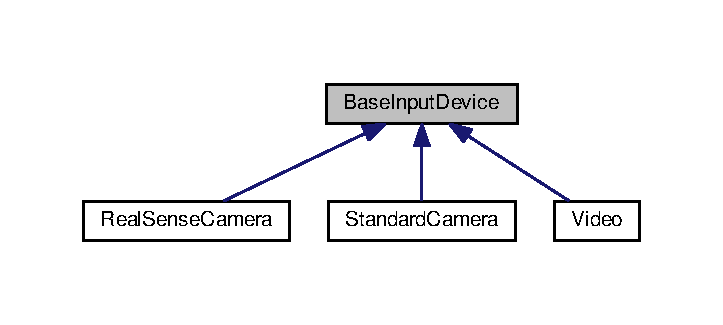
\includegraphics[width=347pt]{classBaseInputDevice__inherit__graph}
\end{center}
\end{figure}
\subsection*{Public Member Functions}
\begin{DoxyCompactItemize}
\item 
virtual bool \hyperlink{classBaseInputDevice_a487cef7725bab9c8cd7141b9b2f83eea}{initialize} ()=0
\begin{DoxyCompactList}\small\item\em initialize the input device, for cameras, it will turn the camera on and get ready to read frames, for videos, it will open a video file \end{DoxyCompactList}\item 
virtual bool \hyperlink{classBaseInputDevice_a7fb82b301d42d63e1b98455eb88ccddd}{initialize} (\hyperlink{CMakeCache_8txt_a79a3d8790b2588b09777910863574e09}{int})=0
\item 
virtual bool \hyperlink{classBaseInputDevice_a8ad1f513052fd4c43e030c3958808bfa}{initialize} (size\+\_\+t width, size\+\_\+t height)=0
\item 
virtual bool \hyperlink{classBaseInputDevice_a49b0a9ff7286d5fb3bccf61a0baaa32a}{read} (cv\+::\+Mat $\ast$frame)=0
\begin{DoxyCompactList}\small\item\em read next frame, and give the value to argument frame \end{DoxyCompactList}\item 
virtual void \hyperlink{classBaseInputDevice_a6f88b6eae38b58dd534f082690f840b3}{config} ()=0
\item 
virtual \hyperlink{classBaseInputDevice_af3f4d01b6e32f62ea6b3d475f12a1a5a}{$\sim$\+Base\+Input\+Device} ()=default
\item 
size\+\_\+t \hyperlink{classBaseInputDevice_a27846cadcc13830798fa92be6800f764}{get\+Width} ()
\item 
void \hyperlink{classBaseInputDevice_a980073308aee4edf67d43a85fdaa2f81}{set\+Width} (size\+\_\+t width)
\item 
size\+\_\+t \hyperlink{classBaseInputDevice_ad38b119a840adacf04c16d75462fc4b7}{get\+Height} ()
\item 
void \hyperlink{classBaseInputDevice_a3312adc6b71bc08da39b5df1be565cef}{set\+Height} (size\+\_\+t height)
\item 
bool \hyperlink{classBaseInputDevice_a560fe86d007739992af04198237909a5}{get\+Is\+Init} ()
\item 
void \hyperlink{classBaseInputDevice_a92e8c0f893c1eb9dcbdd7fb38daf5da1}{set\+Is\+Init} (bool is\+\_\+init)
\end{DoxyCompactItemize}


\subsection{Detailed Description}
This class is an interface for three kinds of input devices\+: realsense camera, standard camera and video. 

Definition at line 16 of file input.\+h.



\subsection{Constructor \& Destructor Documentation}
\index{Base\+Input\+Device@{Base\+Input\+Device}!````~Base\+Input\+Device@{$\sim$\+Base\+Input\+Device}}
\index{````~Base\+Input\+Device@{$\sim$\+Base\+Input\+Device}!Base\+Input\+Device@{Base\+Input\+Device}}
\subsubsection[{\texorpdfstring{$\sim$\+Base\+Input\+Device()=default}{~BaseInputDevice()=default}}]{\setlength{\rightskip}{0pt plus 5cm}virtual Base\+Input\+Device\+::$\sim$\+Base\+Input\+Device (
\begin{DoxyParamCaption}
{}
\end{DoxyParamCaption}
)\hspace{0.3cm}{\ttfamily [virtual]}, {\ttfamily [default]}}\hypertarget{classBaseInputDevice_af3f4d01b6e32f62ea6b3d475f12a1a5a}{}\label{classBaseInputDevice_af3f4d01b6e32f62ea6b3d475f12a1a5a}


\subsection{Member Function Documentation}
\index{Base\+Input\+Device@{Base\+Input\+Device}!config@{config}}
\index{config@{config}!Base\+Input\+Device@{Base\+Input\+Device}}
\subsubsection[{\texorpdfstring{config()=0}{config()=0}}]{\setlength{\rightskip}{0pt plus 5cm}virtual void Base\+Input\+Device\+::config (
\begin{DoxyParamCaption}
{}
\end{DoxyParamCaption}
)\hspace{0.3cm}{\ttfamily [pure virtual]}}\hypertarget{classBaseInputDevice_a6f88b6eae38b58dd534f082690f840b3}{}\label{classBaseInputDevice_a6f88b6eae38b58dd534f082690f840b3}


Implemented in \hyperlink{classVideo_a027d05e5a0391601cb0fea11a063a957}{Video}, \hyperlink{classStandardCamera_a728cfa57a28a8683d9f05a983aae6caa}{Standard\+Camera}, and \hyperlink{classRealSenseCamera_aa701d355ffa10f58d664201523097486}{Real\+Sense\+Camera}.

\index{Base\+Input\+Device@{Base\+Input\+Device}!get\+Height@{get\+Height}}
\index{get\+Height@{get\+Height}!Base\+Input\+Device@{Base\+Input\+Device}}
\subsubsection[{\texorpdfstring{get\+Height()}{getHeight()}}]{\setlength{\rightskip}{0pt plus 5cm}size\+\_\+t Base\+Input\+Device\+::get\+Height (
\begin{DoxyParamCaption}
{}
\end{DoxyParamCaption}
)\hspace{0.3cm}{\ttfamily [inline]}}\hypertarget{classBaseInputDevice_ad38b119a840adacf04c16d75462fc4b7}{}\label{classBaseInputDevice_ad38b119a840adacf04c16d75462fc4b7}


Definition at line 37 of file input.\+h.


\begin{DoxyCode}
37 \{ \textcolor{keywordflow}{return} height\_; \}
\end{DoxyCode}
\index{Base\+Input\+Device@{Base\+Input\+Device}!get\+Is\+Init@{get\+Is\+Init}}
\index{get\+Is\+Init@{get\+Is\+Init}!Base\+Input\+Device@{Base\+Input\+Device}}
\subsubsection[{\texorpdfstring{get\+Is\+Init()}{getIsInit()}}]{\setlength{\rightskip}{0pt plus 5cm}bool Base\+Input\+Device\+::get\+Is\+Init (
\begin{DoxyParamCaption}
{}
\end{DoxyParamCaption}
)\hspace{0.3cm}{\ttfamily [inline]}}\hypertarget{classBaseInputDevice_a560fe86d007739992af04198237909a5}{}\label{classBaseInputDevice_a560fe86d007739992af04198237909a5}


Definition at line 39 of file input.\+h.


\begin{DoxyCode}
39 \{ \textcolor{keywordflow}{return} is\_init\_; \}
\end{DoxyCode}
\index{Base\+Input\+Device@{Base\+Input\+Device}!get\+Width@{get\+Width}}
\index{get\+Width@{get\+Width}!Base\+Input\+Device@{Base\+Input\+Device}}
\subsubsection[{\texorpdfstring{get\+Width()}{getWidth()}}]{\setlength{\rightskip}{0pt plus 5cm}size\+\_\+t Base\+Input\+Device\+::get\+Width (
\begin{DoxyParamCaption}
{}
\end{DoxyParamCaption}
)\hspace{0.3cm}{\ttfamily [inline]}}\hypertarget{classBaseInputDevice_a27846cadcc13830798fa92be6800f764}{}\label{classBaseInputDevice_a27846cadcc13830798fa92be6800f764}


Definition at line 35 of file input.\+h.


\begin{DoxyCode}
35 \{ \textcolor{keywordflow}{return} width\_; \}
\end{DoxyCode}
\index{Base\+Input\+Device@{Base\+Input\+Device}!initialize@{initialize}}
\index{initialize@{initialize}!Base\+Input\+Device@{Base\+Input\+Device}}
\subsubsection[{\texorpdfstring{initialize()=0}{initialize()=0}}]{\setlength{\rightskip}{0pt plus 5cm}virtual bool Base\+Input\+Device\+::initialize (
\begin{DoxyParamCaption}
{}
\end{DoxyParamCaption}
)\hspace{0.3cm}{\ttfamily [pure virtual]}}\hypertarget{classBaseInputDevice_a487cef7725bab9c8cd7141b9b2f83eea}{}\label{classBaseInputDevice_a487cef7725bab9c8cd7141b9b2f83eea}


initialize the input device, for cameras, it will turn the camera on and get ready to read frames, for videos, it will open a video file 

\begin{DoxyReturn}{Returns}
whether the input device is successfully turned on 
\end{DoxyReturn}


Implemented in \hyperlink{classVideo_a276f977e85c9f6815d4d0419d59285bd}{Video}, \hyperlink{classStandardCamera_ae748ec2c2cc35897391b0dacc78140f3}{Standard\+Camera}, and \hyperlink{classRealSenseCamera_abef31b3c9da59cc9071d3ab5b91d5722}{Real\+Sense\+Camera}.

\index{Base\+Input\+Device@{Base\+Input\+Device}!initialize@{initialize}}
\index{initialize@{initialize}!Base\+Input\+Device@{Base\+Input\+Device}}
\subsubsection[{\texorpdfstring{initialize(int)=0}{initialize(int)=0}}]{\setlength{\rightskip}{0pt plus 5cm}virtual bool Base\+Input\+Device\+::initialize (
\begin{DoxyParamCaption}
\item[{{\bf int}}]{}
\end{DoxyParamCaption}
)\hspace{0.3cm}{\ttfamily [pure virtual]}}\hypertarget{classBaseInputDevice_a7fb82b301d42d63e1b98455eb88ccddd}{}\label{classBaseInputDevice_a7fb82b301d42d63e1b98455eb88ccddd}


Implemented in \hyperlink{classVideo_a70f040b7eb1e967f9fb52d5fb866814a}{Video}, \hyperlink{classStandardCamera_ac6060f251351e98c0d1f9066f197cf3a}{Standard\+Camera}, and \hyperlink{classRealSenseCamera_a258741364cc8e535f16a9995bc067c0e}{Real\+Sense\+Camera}.

\index{Base\+Input\+Device@{Base\+Input\+Device}!initialize@{initialize}}
\index{initialize@{initialize}!Base\+Input\+Device@{Base\+Input\+Device}}
\subsubsection[{\texorpdfstring{initialize(size\+\_\+t width, size\+\_\+t height)=0}{initialize(size_t width, size_t height)=0}}]{\setlength{\rightskip}{0pt plus 5cm}virtual bool Base\+Input\+Device\+::initialize (
\begin{DoxyParamCaption}
\item[{size\+\_\+t}]{width, }
\item[{size\+\_\+t}]{height}
\end{DoxyParamCaption}
)\hspace{0.3cm}{\ttfamily [pure virtual]}}\hypertarget{classBaseInputDevice_a8ad1f513052fd4c43e030c3958808bfa}{}\label{classBaseInputDevice_a8ad1f513052fd4c43e030c3958808bfa}


Implemented in \hyperlink{classVideo_a5c1a49fb9e4151123b9e4721f31f55ec}{Video}, \hyperlink{classStandardCamera_a1d7f1c06cff1a76ed2c951cf6d3e2efa}{Standard\+Camera}, and \hyperlink{classRealSenseCamera_a347e9d320a3e42dccf60b3433c00ccd1}{Real\+Sense\+Camera}.

\index{Base\+Input\+Device@{Base\+Input\+Device}!read@{read}}
\index{read@{read}!Base\+Input\+Device@{Base\+Input\+Device}}
\subsubsection[{\texorpdfstring{read(cv\+::\+Mat $\ast$frame)=0}{read(cv::Mat *frame)=0}}]{\setlength{\rightskip}{0pt plus 5cm}virtual bool Base\+Input\+Device\+::read (
\begin{DoxyParamCaption}
\item[{cv\+::\+Mat $\ast$}]{frame}
\end{DoxyParamCaption}
)\hspace{0.3cm}{\ttfamily [pure virtual]}}\hypertarget{classBaseInputDevice_a49b0a9ff7286d5fb3bccf61a0baaa32a}{}\label{classBaseInputDevice_a49b0a9ff7286d5fb3bccf61a0baaa32a}


read next frame, and give the value to argument frame 

\begin{DoxyReturn}{Returns}
whether the next frame is successfully read 
\end{DoxyReturn}


Implemented in \hyperlink{classVideo_a4653f5a44dc2697e6d2093353f8e2be8}{Video}, \hyperlink{classStandardCamera_ac0e08505998e2f0f21ab8120b6f8cf5b}{Standard\+Camera}, and \hyperlink{classRealSenseCamera_ad64fc570435b61d47f349e6f0636085a}{Real\+Sense\+Camera}.

\index{Base\+Input\+Device@{Base\+Input\+Device}!set\+Height@{set\+Height}}
\index{set\+Height@{set\+Height}!Base\+Input\+Device@{Base\+Input\+Device}}
\subsubsection[{\texorpdfstring{set\+Height(size\+\_\+t height)}{setHeight(size_t height)}}]{\setlength{\rightskip}{0pt plus 5cm}void Base\+Input\+Device\+::set\+Height (
\begin{DoxyParamCaption}
\item[{size\+\_\+t}]{height}
\end{DoxyParamCaption}
)\hspace{0.3cm}{\ttfamily [inline]}}\hypertarget{classBaseInputDevice_a3312adc6b71bc08da39b5df1be565cef}{}\label{classBaseInputDevice_a3312adc6b71bc08da39b5df1be565cef}


Definition at line 38 of file input.\+h.


\begin{DoxyCode}
38 \{ height\_ = height; \}
\end{DoxyCode}
\index{Base\+Input\+Device@{Base\+Input\+Device}!set\+Is\+Init@{set\+Is\+Init}}
\index{set\+Is\+Init@{set\+Is\+Init}!Base\+Input\+Device@{Base\+Input\+Device}}
\subsubsection[{\texorpdfstring{set\+Is\+Init(bool is\+\_\+init)}{setIsInit(bool is_init)}}]{\setlength{\rightskip}{0pt plus 5cm}void Base\+Input\+Device\+::set\+Is\+Init (
\begin{DoxyParamCaption}
\item[{bool}]{is\+\_\+init}
\end{DoxyParamCaption}
)\hspace{0.3cm}{\ttfamily [inline]}}\hypertarget{classBaseInputDevice_a92e8c0f893c1eb9dcbdd7fb38daf5da1}{}\label{classBaseInputDevice_a92e8c0f893c1eb9dcbdd7fb38daf5da1}


Definition at line 40 of file input.\+h.


\begin{DoxyCode}
40 \{ is\_init\_ = is\_init; \}
\end{DoxyCode}
\index{Base\+Input\+Device@{Base\+Input\+Device}!set\+Width@{set\+Width}}
\index{set\+Width@{set\+Width}!Base\+Input\+Device@{Base\+Input\+Device}}
\subsubsection[{\texorpdfstring{set\+Width(size\+\_\+t width)}{setWidth(size_t width)}}]{\setlength{\rightskip}{0pt plus 5cm}void Base\+Input\+Device\+::set\+Width (
\begin{DoxyParamCaption}
\item[{size\+\_\+t}]{width}
\end{DoxyParamCaption}
)\hspace{0.3cm}{\ttfamily [inline]}}\hypertarget{classBaseInputDevice_a980073308aee4edf67d43a85fdaa2f81}{}\label{classBaseInputDevice_a980073308aee4edf67d43a85fdaa2f81}


Definition at line 36 of file input.\+h.


\begin{DoxyCode}
36 \{ width\_ = width; \}
\end{DoxyCode}


The documentation for this class was generated from the following file\+:\begin{DoxyCompactItemize}
\item 
include/openvino\+\_\+service/inputs/\hyperlink{input_8h}{input.\+h}\end{DoxyCompactItemize}

\hypertarget{classBaseOutput}{}\section{Base\+Output Class Reference}
\label{classBaseOutput}\index{Base\+Output@{Base\+Output}}


This class is a base class for various output devices. It employs visitor pattern to perform different operations to different inference result with different output device.  




{\ttfamily \#include $<$output.\+h$>$}



Inheritance diagram for Base\+Output\+:
\nopagebreak
\begin{figure}[H]
\begin{center}
\leavevmode
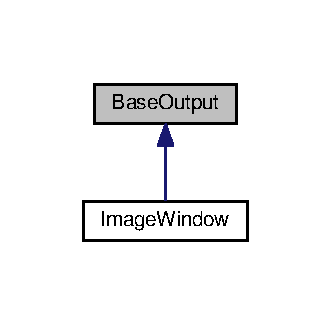
\includegraphics[width=159pt]{classBaseOutput__inherit__graph}
\end{center}
\end{figure}
\subsection*{Public Member Functions}
\begin{DoxyCompactItemize}
\item 
\hyperlink{classBaseOutput_ae88037c3f5a3bd416f3a64e756c75102}{Base\+Output} ()=default
\item 
virtual void \hyperlink{classBaseOutput_ac8e9c0077758e64648fd1bd28661dec7}{prepare\+Data} (const \hyperlink{structInferenceResult_1_1FaceDetectionResult}{Inference\+Result\+::\+Face\+Detection\+Result} \&)=0
\item 
virtual void \hyperlink{classBaseOutput_a67d7a495441233da42b134667a312202}{prepare\+Data} (const \hyperlink{structInferenceResult_1_1EmotionsResult}{Inference\+Result\+::\+Emotions\+Result} \&)=0
\item 
virtual void \hyperlink{classBaseOutput_a6a51c16ebfd7a58829bfa675e562b8f1}{prepare\+Data} (const \hyperlink{structInferenceResult_1_1AgeGenderResult}{Inference\+Result\+::\+Age\+Gender\+Result} \&)=0
\item 
virtual void \hyperlink{classBaseOutput_a3549ade1424963fff201fd946075fd4e}{prepare\+Data} (const \hyperlink{structInferenceResult_1_1HeadPoseResult}{Inference\+Result\+::\+Head\+Pose\+Result} \&)=0
\item 
virtual void \hyperlink{classBaseOutput_ac516cfd7a05af7d710b5dd44d5b79878}{handle\+Output} (const std\+::string \&overall\+\_\+output\+\_\+text)=0
\item 
virtual void \hyperlink{classBaseOutput_acdcbc58abecbf5671b1705937cd1cf02}{feed\+Frame} (const cv\+::\+Mat \&frame)
\end{DoxyCompactItemize}


\subsection{Detailed Description}
This class is a base class for various output devices. It employs visitor pattern to perform different operations to different inference result with different output device. 

Definition at line 19 of file output.\+h.



\subsection{Constructor \& Destructor Documentation}
\index{Base\+Output@{Base\+Output}!Base\+Output@{Base\+Output}}
\index{Base\+Output@{Base\+Output}!Base\+Output@{Base\+Output}}
\subsubsection[{\texorpdfstring{Base\+Output()=default}{BaseOutput()=default}}]{\setlength{\rightskip}{0pt plus 5cm}Base\+Output\+::\+Base\+Output (
\begin{DoxyParamCaption}
{}
\end{DoxyParamCaption}
)\hspace{0.3cm}{\ttfamily [default]}}\hypertarget{classBaseOutput_ae88037c3f5a3bd416f3a64e756c75102}{}\label{classBaseOutput_ae88037c3f5a3bd416f3a64e756c75102}


\subsection{Member Function Documentation}
\index{Base\+Output@{Base\+Output}!feed\+Frame@{feed\+Frame}}
\index{feed\+Frame@{feed\+Frame}!Base\+Output@{Base\+Output}}
\subsubsection[{\texorpdfstring{feed\+Frame(const cv\+::\+Mat \&frame)}{feedFrame(const cv::Mat &frame)}}]{\setlength{\rightskip}{0pt plus 5cm}virtual void Base\+Output\+::feed\+Frame (
\begin{DoxyParamCaption}
\item[{const cv\+::\+Mat \&}]{frame}
\end{DoxyParamCaption}
)\hspace{0.3cm}{\ttfamily [inline]}, {\ttfamily [virtual]}}\hypertarget{classBaseOutput_acdcbc58abecbf5671b1705937cd1cf02}{}\label{classBaseOutput_acdcbc58abecbf5671b1705937cd1cf02}


Reimplemented in \hyperlink{classImageWindow_a802e96acaba82b2f83eb3184c702fbcc}{Image\+Window}.



Definition at line 27 of file output.\+h.


\begin{DoxyCode}
27 \{\}
\end{DoxyCode}
\index{Base\+Output@{Base\+Output}!handle\+Output@{handle\+Output}}
\index{handle\+Output@{handle\+Output}!Base\+Output@{Base\+Output}}
\subsubsection[{\texorpdfstring{handle\+Output(const std\+::string \&overall\+\_\+output\+\_\+text)=0}{handleOutput(const std::string &overall_output_text)=0}}]{\setlength{\rightskip}{0pt plus 5cm}virtual void Base\+Output\+::handle\+Output (
\begin{DoxyParamCaption}
\item[{const std\+::string \&}]{overall\+\_\+output\+\_\+text}
\end{DoxyParamCaption}
)\hspace{0.3cm}{\ttfamily [pure virtual]}}\hypertarget{classBaseOutput_ac516cfd7a05af7d710b5dd44d5b79878}{}\label{classBaseOutput_ac516cfd7a05af7d710b5dd44d5b79878}


Implemented in \hyperlink{classImageWindow_a2927e0003c1f4579fb59aff50a9c7de3}{Image\+Window}.

\index{Base\+Output@{Base\+Output}!prepare\+Data@{prepare\+Data}}
\index{prepare\+Data@{prepare\+Data}!Base\+Output@{Base\+Output}}
\subsubsection[{\texorpdfstring{prepare\+Data(const Inference\+Result\+::\+Face\+Detection\+Result \&)=0}{prepareData(const InferenceResult::FaceDetectionResult &)=0}}]{\setlength{\rightskip}{0pt plus 5cm}virtual void Base\+Output\+::prepare\+Data (
\begin{DoxyParamCaption}
\item[{const {\bf Inference\+Result\+::\+Face\+Detection\+Result} \&}]{}
\end{DoxyParamCaption}
)\hspace{0.3cm}{\ttfamily [pure virtual]}}\hypertarget{classBaseOutput_ac8e9c0077758e64648fd1bd28661dec7}{}\label{classBaseOutput_ac8e9c0077758e64648fd1bd28661dec7}


Implemented in \hyperlink{classImageWindow_a26fa3309cf79914dfe09b3b42b85e49e}{Image\+Window}.

\index{Base\+Output@{Base\+Output}!prepare\+Data@{prepare\+Data}}
\index{prepare\+Data@{prepare\+Data}!Base\+Output@{Base\+Output}}
\subsubsection[{\texorpdfstring{prepare\+Data(const Inference\+Result\+::\+Emotions\+Result \&)=0}{prepareData(const InferenceResult::EmotionsResult &)=0}}]{\setlength{\rightskip}{0pt plus 5cm}virtual void Base\+Output\+::prepare\+Data (
\begin{DoxyParamCaption}
\item[{const {\bf Inference\+Result\+::\+Emotions\+Result} \&}]{}
\end{DoxyParamCaption}
)\hspace{0.3cm}{\ttfamily [pure virtual]}}\hypertarget{classBaseOutput_a67d7a495441233da42b134667a312202}{}\label{classBaseOutput_a67d7a495441233da42b134667a312202}


Implemented in \hyperlink{classImageWindow_a4fdaf7f1728e60672c22ddf57a4071b1}{Image\+Window}.

\index{Base\+Output@{Base\+Output}!prepare\+Data@{prepare\+Data}}
\index{prepare\+Data@{prepare\+Data}!Base\+Output@{Base\+Output}}
\subsubsection[{\texorpdfstring{prepare\+Data(const Inference\+Result\+::\+Age\+Gender\+Result \&)=0}{prepareData(const InferenceResult::AgeGenderResult &)=0}}]{\setlength{\rightskip}{0pt plus 5cm}virtual void Base\+Output\+::prepare\+Data (
\begin{DoxyParamCaption}
\item[{const {\bf Inference\+Result\+::\+Age\+Gender\+Result} \&}]{}
\end{DoxyParamCaption}
)\hspace{0.3cm}{\ttfamily [pure virtual]}}\hypertarget{classBaseOutput_a6a51c16ebfd7a58829bfa675e562b8f1}{}\label{classBaseOutput_a6a51c16ebfd7a58829bfa675e562b8f1}


Implemented in \hyperlink{classImageWindow_a09a86f7b0c0e0eec807a4e1458a057c1}{Image\+Window}.

\index{Base\+Output@{Base\+Output}!prepare\+Data@{prepare\+Data}}
\index{prepare\+Data@{prepare\+Data}!Base\+Output@{Base\+Output}}
\subsubsection[{\texorpdfstring{prepare\+Data(const Inference\+Result\+::\+Head\+Pose\+Result \&)=0}{prepareData(const InferenceResult::HeadPoseResult &)=0}}]{\setlength{\rightskip}{0pt plus 5cm}virtual void Base\+Output\+::prepare\+Data (
\begin{DoxyParamCaption}
\item[{const {\bf Inference\+Result\+::\+Head\+Pose\+Result} \&}]{}
\end{DoxyParamCaption}
)\hspace{0.3cm}{\ttfamily [pure virtual]}}\hypertarget{classBaseOutput_a3549ade1424963fff201fd946075fd4e}{}\label{classBaseOutput_a3549ade1424963fff201fd946075fd4e}


Implemented in \hyperlink{classImageWindow_abb0b9b0c103ec0460a2cbeee414b53c4}{Image\+Window}.



The documentation for this class was generated from the following file\+:\begin{DoxyCompactItemize}
\item 
include/openvino\+\_\+service/outputs/\hyperlink{output_8h}{output.\+h}\end{DoxyCompactItemize}

\hypertarget{classColor}{}\section{Color Class Reference}
\label{classColor}\index{Color@{Color}}


A \hyperlink{classColor}{Color} class stores channels of a given color.  




{\ttfamily \#include $<$common.\+hpp$>$}

\subsection*{Public Member Functions}
\begin{DoxyCompactItemize}
\item 
\hyperlink{classColor_a01fc8b90de599a12365e87b9a0719264}{Color} (unsigned \hyperlink{CMakeCache_8txt_afe71f11dacb15682cdc012f7208e6e09}{char} r, unsigned \hyperlink{CMakeCache_8txt_afe71f11dacb15682cdc012f7208e6e09}{char} g, unsigned \hyperlink{CMakeCache_8txt_afe71f11dacb15682cdc012f7208e6e09}{char} b)
\item 
unsigned \hyperlink{CMakeCache_8txt_afe71f11dacb15682cdc012f7208e6e09}{char} \hyperlink{classColor_a2f9d30801b6b81186cad649bb625b98f}{red} ()
\item 
unsigned \hyperlink{CMakeCache_8txt_afe71f11dacb15682cdc012f7208e6e09}{char} \hyperlink{classColor_ad03144614edc7c54fd0fe0132af47213}{blue} ()
\item 
unsigned \hyperlink{CMakeCache_8txt_afe71f11dacb15682cdc012f7208e6e09}{char} \hyperlink{classColor_aca8e95502aec09dfc92a09087bf62990}{green} ()
\end{DoxyCompactItemize}


\subsection{Detailed Description}
A \hyperlink{classColor}{Color} class stores channels of a given color. 

Definition at line 235 of file common.\+hpp.



\subsection{Constructor \& Destructor Documentation}
\index{Color@{Color}!Color@{Color}}
\index{Color@{Color}!Color@{Color}}
\subsubsection[{\texorpdfstring{Color(unsigned char r, unsigned char g, unsigned char b)}{Color(unsigned char r, unsigned char g, unsigned char b)}}]{\setlength{\rightskip}{0pt plus 5cm}Color\+::\+Color (
\begin{DoxyParamCaption}
\item[{unsigned {\bf char}}]{r, }
\item[{unsigned {\bf char}}]{g, }
\item[{unsigned {\bf char}}]{b}
\end{DoxyParamCaption}
)\hspace{0.3cm}{\ttfamily [inline]}}\hypertarget{classColor_a01fc8b90de599a12365e87b9a0719264}{}\label{classColor_a01fc8b90de599a12365e87b9a0719264}
A default constructor. 
\begin{DoxyParams}{Parameters}
{\em r} & -\/ value for red channel \\
\hline
{\em g} & -\/ value for green channel \\
\hline
{\em b} & -\/ value for blue channel \\
\hline
\end{DoxyParams}


Definition at line 248 of file common.\+hpp.


\begin{DoxyCode}
250                            : \_r(r), \_g(g), \_b(b) \{\}
\end{DoxyCode}


\subsection{Member Function Documentation}
\index{Color@{Color}!blue@{blue}}
\index{blue@{blue}!Color@{Color}}
\subsubsection[{\texorpdfstring{blue()}{blue()}}]{\setlength{\rightskip}{0pt plus 5cm}unsigned {\bf char} Color\+::blue (
\begin{DoxyParamCaption}
{}
\end{DoxyParamCaption}
)\hspace{0.3cm}{\ttfamily [inline]}}\hypertarget{classColor_ad03144614edc7c54fd0fe0132af47213}{}\label{classColor_ad03144614edc7c54fd0fe0132af47213}


Definition at line 256 of file common.\+hpp.


\begin{DoxyCode}
256                                 \{
257         \textcolor{keywordflow}{return} \_b;
258     \}
\end{DoxyCode}
\index{Color@{Color}!green@{green}}
\index{green@{green}!Color@{Color}}
\subsubsection[{\texorpdfstring{green()}{green()}}]{\setlength{\rightskip}{0pt plus 5cm}unsigned {\bf char} Color\+::green (
\begin{DoxyParamCaption}
{}
\end{DoxyParamCaption}
)\hspace{0.3cm}{\ttfamily [inline]}}\hypertarget{classColor_aca8e95502aec09dfc92a09087bf62990}{}\label{classColor_aca8e95502aec09dfc92a09087bf62990}


Definition at line 260 of file common.\+hpp.


\begin{DoxyCode}
260                                  \{
261         \textcolor{keywordflow}{return} \_g;
262     \}
\end{DoxyCode}
\index{Color@{Color}!red@{red}}
\index{red@{red}!Color@{Color}}
\subsubsection[{\texorpdfstring{red()}{red()}}]{\setlength{\rightskip}{0pt plus 5cm}unsigned {\bf char} Color\+::red (
\begin{DoxyParamCaption}
{}
\end{DoxyParamCaption}
)\hspace{0.3cm}{\ttfamily [inline]}}\hypertarget{classColor_a2f9d30801b6b81186cad649bb625b98f}{}\label{classColor_a2f9d30801b6b81186cad649bb625b98f}


Definition at line 252 of file common.\+hpp.


\begin{DoxyCode}
252                                \{
253         \textcolor{keywordflow}{return} \_r;
254     \}
\end{DoxyCode}


The documentation for this class was generated from the following file\+:\begin{DoxyCompactItemize}
\item 
include/openvino\+\_\+service/\hyperlink{common_8hpp}{common.\+hpp}\end{DoxyCompactItemize}

\hypertarget{structGFLAGS__NAMESPACE_1_1CommandLineFlagInfo}{}\section{G\+F\+L\+A\+G\+S\+\_\+\+N\+A\+M\+E\+S\+P\+A\+CE\+:\+:Command\+Line\+Flag\+Info Struct Reference}
\label{structGFLAGS__NAMESPACE_1_1CommandLineFlagInfo}\index{G\+F\+L\+A\+G\+S\+\_\+\+N\+A\+M\+E\+S\+P\+A\+C\+E\+::\+Command\+Line\+Flag\+Info@{G\+F\+L\+A\+G\+S\+\_\+\+N\+A\+M\+E\+S\+P\+A\+C\+E\+::\+Command\+Line\+Flag\+Info}}


{\ttfamily \#include $<$gflags.\+h$>$}



Collaboration diagram for G\+F\+L\+A\+G\+S\+\_\+\+N\+A\+M\+E\+S\+P\+A\+CE\+:\+:Command\+Line\+Flag\+Info\+:
\nopagebreak
\begin{figure}[H]
\begin{center}
\leavevmode
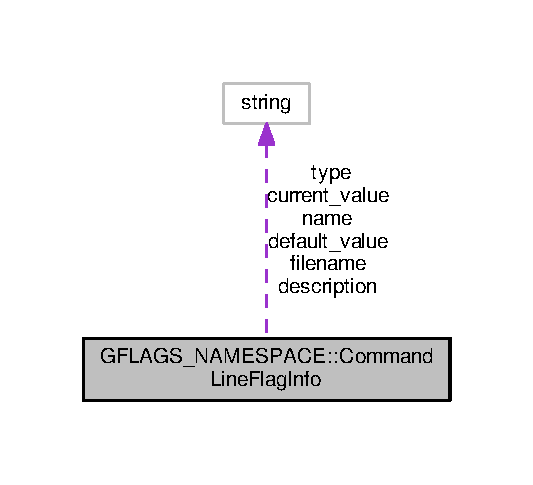
\includegraphics[width=256pt]{structGFLAGS__NAMESPACE_1_1CommandLineFlagInfo__coll__graph}
\end{center}
\end{figure}
\subsection*{Public Attributes}
\begin{DoxyCompactItemize}
\item 
std\+::string \hyperlink{structGFLAGS__NAMESPACE_1_1CommandLineFlagInfo_af56a81d2c7aca29203746976004abfc2}{name}
\item 
std\+::string \hyperlink{structGFLAGS__NAMESPACE_1_1CommandLineFlagInfo_a04f02cad9caae94a7ffd88e9cb89585b}{type}
\item 
std\+::string \hyperlink{structGFLAGS__NAMESPACE_1_1CommandLineFlagInfo_ae8bdcd07b1cb5b0561e122af6955fc90}{description}
\item 
std\+::string \hyperlink{structGFLAGS__NAMESPACE_1_1CommandLineFlagInfo_a654abe3f7f744c9b3772c78bb8a4e90e}{current\+\_\+value}
\item 
std\+::string \hyperlink{structGFLAGS__NAMESPACE_1_1CommandLineFlagInfo_a6f786f24cd6eaba82158e785809f53de}{default\+\_\+value}
\item 
std\+::string \hyperlink{structGFLAGS__NAMESPACE_1_1CommandLineFlagInfo_af889e5db7ce96fd27b34bd9cc6bfaa8c}{filename}
\item 
bool \hyperlink{structGFLAGS__NAMESPACE_1_1CommandLineFlagInfo_a0942bc076c1307b2ab7f3c6d6c7ae4c3}{has\+\_\+validator\+\_\+fn}
\item 
bool \hyperlink{structGFLAGS__NAMESPACE_1_1CommandLineFlagInfo_a9c9ae9de1ba9e9b591c21a761f9f08c2}{is\+\_\+default}
\item 
const void $\ast$ \hyperlink{structGFLAGS__NAMESPACE_1_1CommandLineFlagInfo_afe83fd3e23c58a6c03197807000e6990}{flag\+\_\+ptr}
\end{DoxyCompactItemize}


\subsection{Detailed Description}


Definition at line 155 of file gflags.\+h.



\subsection{Member Data Documentation}
\index{G\+F\+L\+A\+G\+S\+\_\+\+N\+A\+M\+E\+S\+P\+A\+C\+E\+::\+Command\+Line\+Flag\+Info@{G\+F\+L\+A\+G\+S\+\_\+\+N\+A\+M\+E\+S\+P\+A\+C\+E\+::\+Command\+Line\+Flag\+Info}!current\+\_\+value@{current\+\_\+value}}
\index{current\+\_\+value@{current\+\_\+value}!G\+F\+L\+A\+G\+S\+\_\+\+N\+A\+M\+E\+S\+P\+A\+C\+E\+::\+Command\+Line\+Flag\+Info@{G\+F\+L\+A\+G\+S\+\_\+\+N\+A\+M\+E\+S\+P\+A\+C\+E\+::\+Command\+Line\+Flag\+Info}}
\subsubsection[{\texorpdfstring{current\+\_\+value}{current_value}}]{\setlength{\rightskip}{0pt plus 5cm}std\+::string G\+F\+L\+A\+G\+S\+\_\+\+N\+A\+M\+E\+S\+P\+A\+C\+E\+::\+Command\+Line\+Flag\+Info\+::current\+\_\+value}\hypertarget{structGFLAGS__NAMESPACE_1_1CommandLineFlagInfo_a654abe3f7f744c9b3772c78bb8a4e90e}{}\label{structGFLAGS__NAMESPACE_1_1CommandLineFlagInfo_a654abe3f7f744c9b3772c78bb8a4e90e}


Definition at line 159 of file gflags.\+h.

\index{G\+F\+L\+A\+G\+S\+\_\+\+N\+A\+M\+E\+S\+P\+A\+C\+E\+::\+Command\+Line\+Flag\+Info@{G\+F\+L\+A\+G\+S\+\_\+\+N\+A\+M\+E\+S\+P\+A\+C\+E\+::\+Command\+Line\+Flag\+Info}!default\+\_\+value@{default\+\_\+value}}
\index{default\+\_\+value@{default\+\_\+value}!G\+F\+L\+A\+G\+S\+\_\+\+N\+A\+M\+E\+S\+P\+A\+C\+E\+::\+Command\+Line\+Flag\+Info@{G\+F\+L\+A\+G\+S\+\_\+\+N\+A\+M\+E\+S\+P\+A\+C\+E\+::\+Command\+Line\+Flag\+Info}}
\subsubsection[{\texorpdfstring{default\+\_\+value}{default_value}}]{\setlength{\rightskip}{0pt plus 5cm}std\+::string G\+F\+L\+A\+G\+S\+\_\+\+N\+A\+M\+E\+S\+P\+A\+C\+E\+::\+Command\+Line\+Flag\+Info\+::default\+\_\+value}\hypertarget{structGFLAGS__NAMESPACE_1_1CommandLineFlagInfo_a6f786f24cd6eaba82158e785809f53de}{}\label{structGFLAGS__NAMESPACE_1_1CommandLineFlagInfo_a6f786f24cd6eaba82158e785809f53de}


Definition at line 160 of file gflags.\+h.

\index{G\+F\+L\+A\+G\+S\+\_\+\+N\+A\+M\+E\+S\+P\+A\+C\+E\+::\+Command\+Line\+Flag\+Info@{G\+F\+L\+A\+G\+S\+\_\+\+N\+A\+M\+E\+S\+P\+A\+C\+E\+::\+Command\+Line\+Flag\+Info}!description@{description}}
\index{description@{description}!G\+F\+L\+A\+G\+S\+\_\+\+N\+A\+M\+E\+S\+P\+A\+C\+E\+::\+Command\+Line\+Flag\+Info@{G\+F\+L\+A\+G\+S\+\_\+\+N\+A\+M\+E\+S\+P\+A\+C\+E\+::\+Command\+Line\+Flag\+Info}}
\subsubsection[{\texorpdfstring{description}{description}}]{\setlength{\rightskip}{0pt plus 5cm}std\+::string G\+F\+L\+A\+G\+S\+\_\+\+N\+A\+M\+E\+S\+P\+A\+C\+E\+::\+Command\+Line\+Flag\+Info\+::description}\hypertarget{structGFLAGS__NAMESPACE_1_1CommandLineFlagInfo_ae8bdcd07b1cb5b0561e122af6955fc90}{}\label{structGFLAGS__NAMESPACE_1_1CommandLineFlagInfo_ae8bdcd07b1cb5b0561e122af6955fc90}


Definition at line 158 of file gflags.\+h.

\index{G\+F\+L\+A\+G\+S\+\_\+\+N\+A\+M\+E\+S\+P\+A\+C\+E\+::\+Command\+Line\+Flag\+Info@{G\+F\+L\+A\+G\+S\+\_\+\+N\+A\+M\+E\+S\+P\+A\+C\+E\+::\+Command\+Line\+Flag\+Info}!filename@{filename}}
\index{filename@{filename}!G\+F\+L\+A\+G\+S\+\_\+\+N\+A\+M\+E\+S\+P\+A\+C\+E\+::\+Command\+Line\+Flag\+Info@{G\+F\+L\+A\+G\+S\+\_\+\+N\+A\+M\+E\+S\+P\+A\+C\+E\+::\+Command\+Line\+Flag\+Info}}
\subsubsection[{\texorpdfstring{filename}{filename}}]{\setlength{\rightskip}{0pt plus 5cm}std\+::string G\+F\+L\+A\+G\+S\+\_\+\+N\+A\+M\+E\+S\+P\+A\+C\+E\+::\+Command\+Line\+Flag\+Info\+::filename}\hypertarget{structGFLAGS__NAMESPACE_1_1CommandLineFlagInfo_af889e5db7ce96fd27b34bd9cc6bfaa8c}{}\label{structGFLAGS__NAMESPACE_1_1CommandLineFlagInfo_af889e5db7ce96fd27b34bd9cc6bfaa8c}


Definition at line 161 of file gflags.\+h.

\index{G\+F\+L\+A\+G\+S\+\_\+\+N\+A\+M\+E\+S\+P\+A\+C\+E\+::\+Command\+Line\+Flag\+Info@{G\+F\+L\+A\+G\+S\+\_\+\+N\+A\+M\+E\+S\+P\+A\+C\+E\+::\+Command\+Line\+Flag\+Info}!flag\+\_\+ptr@{flag\+\_\+ptr}}
\index{flag\+\_\+ptr@{flag\+\_\+ptr}!G\+F\+L\+A\+G\+S\+\_\+\+N\+A\+M\+E\+S\+P\+A\+C\+E\+::\+Command\+Line\+Flag\+Info@{G\+F\+L\+A\+G\+S\+\_\+\+N\+A\+M\+E\+S\+P\+A\+C\+E\+::\+Command\+Line\+Flag\+Info}}
\subsubsection[{\texorpdfstring{flag\+\_\+ptr}{flag_ptr}}]{\setlength{\rightskip}{0pt plus 5cm}const void$\ast$ G\+F\+L\+A\+G\+S\+\_\+\+N\+A\+M\+E\+S\+P\+A\+C\+E\+::\+Command\+Line\+Flag\+Info\+::flag\+\_\+ptr}\hypertarget{structGFLAGS__NAMESPACE_1_1CommandLineFlagInfo_afe83fd3e23c58a6c03197807000e6990}{}\label{structGFLAGS__NAMESPACE_1_1CommandLineFlagInfo_afe83fd3e23c58a6c03197807000e6990}


Definition at line 166 of file gflags.\+h.

\index{G\+F\+L\+A\+G\+S\+\_\+\+N\+A\+M\+E\+S\+P\+A\+C\+E\+::\+Command\+Line\+Flag\+Info@{G\+F\+L\+A\+G\+S\+\_\+\+N\+A\+M\+E\+S\+P\+A\+C\+E\+::\+Command\+Line\+Flag\+Info}!has\+\_\+validator\+\_\+fn@{has\+\_\+validator\+\_\+fn}}
\index{has\+\_\+validator\+\_\+fn@{has\+\_\+validator\+\_\+fn}!G\+F\+L\+A\+G\+S\+\_\+\+N\+A\+M\+E\+S\+P\+A\+C\+E\+::\+Command\+Line\+Flag\+Info@{G\+F\+L\+A\+G\+S\+\_\+\+N\+A\+M\+E\+S\+P\+A\+C\+E\+::\+Command\+Line\+Flag\+Info}}
\subsubsection[{\texorpdfstring{has\+\_\+validator\+\_\+fn}{has_validator_fn}}]{\setlength{\rightskip}{0pt plus 5cm}bool G\+F\+L\+A\+G\+S\+\_\+\+N\+A\+M\+E\+S\+P\+A\+C\+E\+::\+Command\+Line\+Flag\+Info\+::has\+\_\+validator\+\_\+fn}\hypertarget{structGFLAGS__NAMESPACE_1_1CommandLineFlagInfo_a0942bc076c1307b2ab7f3c6d6c7ae4c3}{}\label{structGFLAGS__NAMESPACE_1_1CommandLineFlagInfo_a0942bc076c1307b2ab7f3c6d6c7ae4c3}


Definition at line 162 of file gflags.\+h.

\index{G\+F\+L\+A\+G\+S\+\_\+\+N\+A\+M\+E\+S\+P\+A\+C\+E\+::\+Command\+Line\+Flag\+Info@{G\+F\+L\+A\+G\+S\+\_\+\+N\+A\+M\+E\+S\+P\+A\+C\+E\+::\+Command\+Line\+Flag\+Info}!is\+\_\+default@{is\+\_\+default}}
\index{is\+\_\+default@{is\+\_\+default}!G\+F\+L\+A\+G\+S\+\_\+\+N\+A\+M\+E\+S\+P\+A\+C\+E\+::\+Command\+Line\+Flag\+Info@{G\+F\+L\+A\+G\+S\+\_\+\+N\+A\+M\+E\+S\+P\+A\+C\+E\+::\+Command\+Line\+Flag\+Info}}
\subsubsection[{\texorpdfstring{is\+\_\+default}{is_default}}]{\setlength{\rightskip}{0pt plus 5cm}bool G\+F\+L\+A\+G\+S\+\_\+\+N\+A\+M\+E\+S\+P\+A\+C\+E\+::\+Command\+Line\+Flag\+Info\+::is\+\_\+default}\hypertarget{structGFLAGS__NAMESPACE_1_1CommandLineFlagInfo_a9c9ae9de1ba9e9b591c21a761f9f08c2}{}\label{structGFLAGS__NAMESPACE_1_1CommandLineFlagInfo_a9c9ae9de1ba9e9b591c21a761f9f08c2}


Definition at line 163 of file gflags.\+h.

\index{G\+F\+L\+A\+G\+S\+\_\+\+N\+A\+M\+E\+S\+P\+A\+C\+E\+::\+Command\+Line\+Flag\+Info@{G\+F\+L\+A\+G\+S\+\_\+\+N\+A\+M\+E\+S\+P\+A\+C\+E\+::\+Command\+Line\+Flag\+Info}!name@{name}}
\index{name@{name}!G\+F\+L\+A\+G\+S\+\_\+\+N\+A\+M\+E\+S\+P\+A\+C\+E\+::\+Command\+Line\+Flag\+Info@{G\+F\+L\+A\+G\+S\+\_\+\+N\+A\+M\+E\+S\+P\+A\+C\+E\+::\+Command\+Line\+Flag\+Info}}
\subsubsection[{\texorpdfstring{name}{name}}]{\setlength{\rightskip}{0pt plus 5cm}std\+::string G\+F\+L\+A\+G\+S\+\_\+\+N\+A\+M\+E\+S\+P\+A\+C\+E\+::\+Command\+Line\+Flag\+Info\+::name}\hypertarget{structGFLAGS__NAMESPACE_1_1CommandLineFlagInfo_af56a81d2c7aca29203746976004abfc2}{}\label{structGFLAGS__NAMESPACE_1_1CommandLineFlagInfo_af56a81d2c7aca29203746976004abfc2}


Definition at line 156 of file gflags.\+h.

\index{G\+F\+L\+A\+G\+S\+\_\+\+N\+A\+M\+E\+S\+P\+A\+C\+E\+::\+Command\+Line\+Flag\+Info@{G\+F\+L\+A\+G\+S\+\_\+\+N\+A\+M\+E\+S\+P\+A\+C\+E\+::\+Command\+Line\+Flag\+Info}!type@{type}}
\index{type@{type}!G\+F\+L\+A\+G\+S\+\_\+\+N\+A\+M\+E\+S\+P\+A\+C\+E\+::\+Command\+Line\+Flag\+Info@{G\+F\+L\+A\+G\+S\+\_\+\+N\+A\+M\+E\+S\+P\+A\+C\+E\+::\+Command\+Line\+Flag\+Info}}
\subsubsection[{\texorpdfstring{type}{type}}]{\setlength{\rightskip}{0pt plus 5cm}std\+::string G\+F\+L\+A\+G\+S\+\_\+\+N\+A\+M\+E\+S\+P\+A\+C\+E\+::\+Command\+Line\+Flag\+Info\+::type}\hypertarget{structGFLAGS__NAMESPACE_1_1CommandLineFlagInfo_a04f02cad9caae94a7ffd88e9cb89585b}{}\label{structGFLAGS__NAMESPACE_1_1CommandLineFlagInfo_a04f02cad9caae94a7ffd88e9cb89585b}


Definition at line 157 of file gflags.\+h.



The documentation for this struct was generated from the following file\+:\begin{DoxyCompactItemize}
\item 
cmake-\/build-\/debug/thirdparty/gflags/include/gflags/\hyperlink{gflags_8h}{gflags.\+h}\end{DoxyCompactItemize}

\hypertarget{structGFLAGS__NAMESPACE_1_1CompileAssert}{}\section{G\+F\+L\+A\+G\+S\+\_\+\+N\+A\+M\+E\+S\+P\+A\+CE\+:\+:Compile\+Assert$<$ b $>$ Struct Template Reference}
\label{structGFLAGS__NAMESPACE_1_1CompileAssert}\index{G\+F\+L\+A\+G\+S\+\_\+\+N\+A\+M\+E\+S\+P\+A\+C\+E\+::\+Compile\+Assert$<$ b $>$@{G\+F\+L\+A\+G\+S\+\_\+\+N\+A\+M\+E\+S\+P\+A\+C\+E\+::\+Compile\+Assert$<$ b $>$}}


{\ttfamily \#include $<$util.\+h$>$}



\subsection{Detailed Description}
\subsubsection*{template$<$bool b$>$\\*
struct G\+F\+L\+A\+G\+S\+\_\+\+N\+A\+M\+E\+S\+P\+A\+C\+E\+::\+Compile\+Assert$<$ b $>$}



Definition at line 90 of file util.\+h.



The documentation for this struct was generated from the following file\+:\begin{DoxyCompactItemize}
\item 
thirdparty/gflags/src/\hyperlink{util_8h}{util.\+h}\end{DoxyCompactItemize}

\hypertarget{structfLB_1_1CompileAssert}{}\section{f\+LB\+:\+:Compile\+Assert Struct Reference}
\label{structfLB_1_1CompileAssert}\index{f\+L\+B\+::\+Compile\+Assert@{f\+L\+B\+::\+Compile\+Assert}}


{\ttfamily \#include $<$gflags.\+h$>$}



\subsection{Detailed Description}


Definition at line 497 of file gflags.\+h.



The documentation for this struct was generated from the following file\+:\begin{DoxyCompactItemize}
\item 
cmake-\/build-\/debug/thirdparty/gflags/include/gflags/\hyperlink{gflags_8h}{gflags.\+h}\end{DoxyCompactItemize}

\hypertarget{structGFLAGS__NAMESPACE_1_1CompileAssert_3_01true_01_4}{}\section{G\+F\+L\+A\+G\+S\+\_\+\+N\+A\+M\+E\+S\+P\+A\+CE\+:\+:Compile\+Assert$<$ true $>$ Struct Template Reference}
\label{structGFLAGS__NAMESPACE_1_1CompileAssert_3_01true_01_4}\index{G\+F\+L\+A\+G\+S\+\_\+\+N\+A\+M\+E\+S\+P\+A\+C\+E\+::\+Compile\+Assert$<$ true $>$@{G\+F\+L\+A\+G\+S\+\_\+\+N\+A\+M\+E\+S\+P\+A\+C\+E\+::\+Compile\+Assert$<$ true $>$}}


{\ttfamily \#include $<$util.\+h$>$}



\subsection{Detailed Description}
\subsubsection*{template$<$$>$\\*
struct G\+F\+L\+A\+G\+S\+\_\+\+N\+A\+M\+E\+S\+P\+A\+C\+E\+::\+Compile\+Assert$<$ true $>$}



Definition at line 91 of file util.\+h.



The documentation for this struct was generated from the following file\+:\begin{DoxyCompactItemize}
\item 
thirdparty/gflags/src/\hyperlink{util_8h}{util.\+h}\end{DoxyCompactItemize}

\hypertarget{structInferenceEngine_1_1Extensions_1_1Cpu_1_1ConfidenceComparator}{}\section{Inference\+Engine\+:\+:Extensions\+:\+:Cpu\+:\+:Confidence\+Comparator Struct Reference}
\label{structInferenceEngine_1_1Extensions_1_1Cpu_1_1ConfidenceComparator}\index{Inference\+Engine\+::\+Extensions\+::\+Cpu\+::\+Confidence\+Comparator@{Inference\+Engine\+::\+Extensions\+::\+Cpu\+::\+Confidence\+Comparator}}
\subsection*{Public Member Functions}
\begin{DoxyCompactItemize}
\item 
\hyperlink{structInferenceEngine_1_1Extensions_1_1Cpu_1_1ConfidenceComparator_a6a64fe84a0a07453cfdfbcbd935e0c05}{Confidence\+Comparator} (const float $\ast$conf\+\_\+data)
\item 
bool \hyperlink{structInferenceEngine_1_1Extensions_1_1Cpu_1_1ConfidenceComparator_a667aec658d4b9b1a1b52672efc46ada8}{operator()} (\hyperlink{CMakeCache_8txt_a79a3d8790b2588b09777910863574e09}{int} idx1, \hyperlink{CMakeCache_8txt_a79a3d8790b2588b09777910863574e09}{int} idx2)
\end{DoxyCompactItemize}
\subsection*{Public Attributes}
\begin{DoxyCompactItemize}
\item 
const float $\ast$ \hyperlink{structInferenceEngine_1_1Extensions_1_1Cpu_1_1ConfidenceComparator_a4799b1ce7bed1246a75811fdf76205c6}{\+\_\+conf\+\_\+data}
\end{DoxyCompactItemize}


\subsection{Detailed Description}


Definition at line 343 of file ext\+\_\+detectionoutput.\+cpp.



\subsection{Constructor \& Destructor Documentation}
\index{Inference\+Engine\+::\+Extensions\+::\+Cpu\+::\+Confidence\+Comparator@{Inference\+Engine\+::\+Extensions\+::\+Cpu\+::\+Confidence\+Comparator}!Confidence\+Comparator@{Confidence\+Comparator}}
\index{Confidence\+Comparator@{Confidence\+Comparator}!Inference\+Engine\+::\+Extensions\+::\+Cpu\+::\+Confidence\+Comparator@{Inference\+Engine\+::\+Extensions\+::\+Cpu\+::\+Confidence\+Comparator}}
\subsubsection[{\texorpdfstring{Confidence\+Comparator(const float $\ast$conf\+\_\+data)}{ConfidenceComparator(const float *conf_data)}}]{\setlength{\rightskip}{0pt plus 5cm}Inference\+Engine\+::\+Extensions\+::\+Cpu\+::\+Confidence\+Comparator\+::\+Confidence\+Comparator (
\begin{DoxyParamCaption}
\item[{const float $\ast$}]{conf\+\_\+data}
\end{DoxyParamCaption}
)\hspace{0.3cm}{\ttfamily [inline]}, {\ttfamily [explicit]}}\hypertarget{structInferenceEngine_1_1Extensions_1_1Cpu_1_1ConfidenceComparator_a6a64fe84a0a07453cfdfbcbd935e0c05}{}\label{structInferenceEngine_1_1Extensions_1_1Cpu_1_1ConfidenceComparator_a6a64fe84a0a07453cfdfbcbd935e0c05}


Definition at line 344 of file ext\+\_\+detectionoutput.\+cpp.


\begin{DoxyCode}
344 : \hyperlink{structInferenceEngine_1_1Extensions_1_1Cpu_1_1ConfidenceComparator_a4799b1ce7bed1246a75811fdf76205c6}{\_conf\_data}(conf\_data) \{\}
\end{DoxyCode}


\subsection{Member Function Documentation}
\index{Inference\+Engine\+::\+Extensions\+::\+Cpu\+::\+Confidence\+Comparator@{Inference\+Engine\+::\+Extensions\+::\+Cpu\+::\+Confidence\+Comparator}!operator()@{operator()}}
\index{operator()@{operator()}!Inference\+Engine\+::\+Extensions\+::\+Cpu\+::\+Confidence\+Comparator@{Inference\+Engine\+::\+Extensions\+::\+Cpu\+::\+Confidence\+Comparator}}
\subsubsection[{\texorpdfstring{operator()(int idx1, int idx2)}{operator()(int idx1, int idx2)}}]{\setlength{\rightskip}{0pt plus 5cm}bool Inference\+Engine\+::\+Extensions\+::\+Cpu\+::\+Confidence\+Comparator\+::operator() (
\begin{DoxyParamCaption}
\item[{{\bf int}}]{idx1, }
\item[{{\bf int}}]{idx2}
\end{DoxyParamCaption}
)\hspace{0.3cm}{\ttfamily [inline]}}\hypertarget{structInferenceEngine_1_1Extensions_1_1Cpu_1_1ConfidenceComparator_a667aec658d4b9b1a1b52672efc46ada8}{}\label{structInferenceEngine_1_1Extensions_1_1Cpu_1_1ConfidenceComparator_a667aec658d4b9b1a1b52672efc46ada8}


Definition at line 346 of file ext\+\_\+detectionoutput.\+cpp.


\begin{DoxyCode}
346                                         \{
347         \textcolor{keywordflow}{if} (\hyperlink{structInferenceEngine_1_1Extensions_1_1Cpu_1_1ConfidenceComparator_a4799b1ce7bed1246a75811fdf76205c6}{\_conf\_data}[idx1] > \hyperlink{structInferenceEngine_1_1Extensions_1_1Cpu_1_1ConfidenceComparator_a4799b1ce7bed1246a75811fdf76205c6}{\_conf\_data}[idx2]) \textcolor{keywordflow}{return} \textcolor{keyword}{true};
348         \textcolor{keywordflow}{if} (\hyperlink{structInferenceEngine_1_1Extensions_1_1Cpu_1_1ConfidenceComparator_a4799b1ce7bed1246a75811fdf76205c6}{\_conf\_data}[idx1] < \hyperlink{structInferenceEngine_1_1Extensions_1_1Cpu_1_1ConfidenceComparator_a4799b1ce7bed1246a75811fdf76205c6}{\_conf\_data}[idx2]) \textcolor{keywordflow}{return} \textcolor{keyword}{false};
349         \textcolor{keywordflow}{return} idx1 < idx2;
350     \}
\end{DoxyCode}


\subsection{Member Data Documentation}
\index{Inference\+Engine\+::\+Extensions\+::\+Cpu\+::\+Confidence\+Comparator@{Inference\+Engine\+::\+Extensions\+::\+Cpu\+::\+Confidence\+Comparator}!\+\_\+conf\+\_\+data@{\+\_\+conf\+\_\+data}}
\index{\+\_\+conf\+\_\+data@{\+\_\+conf\+\_\+data}!Inference\+Engine\+::\+Extensions\+::\+Cpu\+::\+Confidence\+Comparator@{Inference\+Engine\+::\+Extensions\+::\+Cpu\+::\+Confidence\+Comparator}}
\subsubsection[{\texorpdfstring{\+\_\+conf\+\_\+data}{_conf_data}}]{\setlength{\rightskip}{0pt plus 5cm}const float$\ast$ Inference\+Engine\+::\+Extensions\+::\+Cpu\+::\+Confidence\+Comparator\+::\+\_\+conf\+\_\+data}\hypertarget{structInferenceEngine_1_1Extensions_1_1Cpu_1_1ConfidenceComparator_a4799b1ce7bed1246a75811fdf76205c6}{}\label{structInferenceEngine_1_1Extensions_1_1Cpu_1_1ConfidenceComparator_a4799b1ce7bed1246a75811fdf76205c6}


Definition at line 352 of file ext\+\_\+detectionoutput.\+cpp.



The documentation for this struct was generated from the following file\+:\begin{DoxyCompactItemize}
\item 
thirdparty/extension/\hyperlink{ext__detectionoutput_8cpp}{ext\+\_\+detectionoutput.\+cpp}\end{DoxyCompactItemize}

\hypertarget{classInferenceEngine_1_1Extensions_1_1Cpu_1_1CTCGreedyDecoderImpl}{}\section{Inference\+Engine\+:\+:Extensions\+:\+:Cpu\+:\+:C\+T\+C\+Greedy\+Decoder\+Impl Class Reference}
\label{classInferenceEngine_1_1Extensions_1_1Cpu_1_1CTCGreedyDecoderImpl}\index{Inference\+Engine\+::\+Extensions\+::\+Cpu\+::\+C\+T\+C\+Greedy\+Decoder\+Impl@{Inference\+Engine\+::\+Extensions\+::\+Cpu\+::\+C\+T\+C\+Greedy\+Decoder\+Impl}}


Inheritance diagram for Inference\+Engine\+:\+:Extensions\+:\+:Cpu\+:\+:C\+T\+C\+Greedy\+Decoder\+Impl\+:
\nopagebreak
\begin{figure}[H]
\begin{center}
\leavevmode
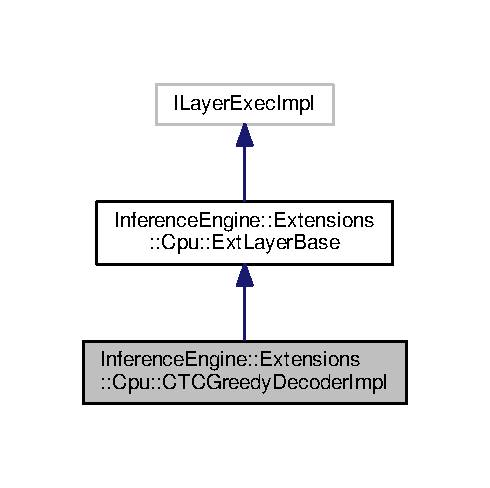
\includegraphics[width=235pt]{classInferenceEngine_1_1Extensions_1_1Cpu_1_1CTCGreedyDecoderImpl__inherit__graph}
\end{center}
\end{figure}


Collaboration diagram for Inference\+Engine\+:\+:Extensions\+:\+:Cpu\+:\+:C\+T\+C\+Greedy\+Decoder\+Impl\+:
\nopagebreak
\begin{figure}[H]
\begin{center}
\leavevmode
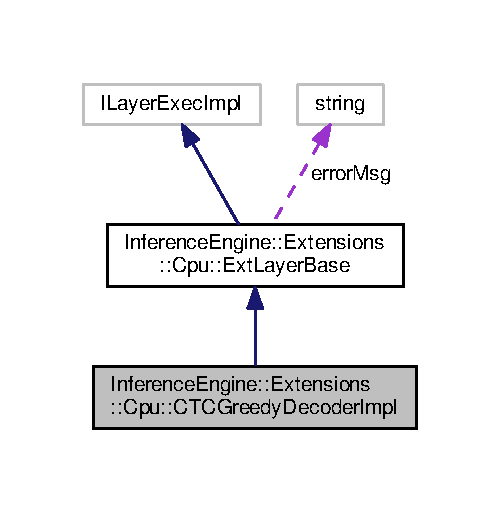
\includegraphics[width=240pt]{classInferenceEngine_1_1Extensions_1_1Cpu_1_1CTCGreedyDecoderImpl__coll__graph}
\end{center}
\end{figure}
\subsection*{Public Member Functions}
\begin{DoxyCompactItemize}
\item 
\hyperlink{classInferenceEngine_1_1Extensions_1_1Cpu_1_1CTCGreedyDecoderImpl_aebd2c0abf6bfdcf39389959637a2465f}{C\+T\+C\+Greedy\+Decoder\+Impl} (const C\+N\+N\+Layer $\ast$layer)
\item 
Status\+Code \hyperlink{classInferenceEngine_1_1Extensions_1_1Cpu_1_1CTCGreedyDecoderImpl_a1a081d08857bf9f13cb49a7d4468e894}{execute} (std\+::vector$<$ Blob\+::\+Ptr $>$ \&inputs, std\+::vector$<$ Blob\+::\+Ptr $>$ \&outputs, Response\+Desc $\ast$resp) noexceptoverride
\end{DoxyCompactItemize}
\subsection*{Additional Inherited Members}


\subsection{Detailed Description}


Definition at line 28 of file ext\+\_\+ctc\+\_\+greedy.\+cpp.



\subsection{Constructor \& Destructor Documentation}
\index{Inference\+Engine\+::\+Extensions\+::\+Cpu\+::\+C\+T\+C\+Greedy\+Decoder\+Impl@{Inference\+Engine\+::\+Extensions\+::\+Cpu\+::\+C\+T\+C\+Greedy\+Decoder\+Impl}!C\+T\+C\+Greedy\+Decoder\+Impl@{C\+T\+C\+Greedy\+Decoder\+Impl}}
\index{C\+T\+C\+Greedy\+Decoder\+Impl@{C\+T\+C\+Greedy\+Decoder\+Impl}!Inference\+Engine\+::\+Extensions\+::\+Cpu\+::\+C\+T\+C\+Greedy\+Decoder\+Impl@{Inference\+Engine\+::\+Extensions\+::\+Cpu\+::\+C\+T\+C\+Greedy\+Decoder\+Impl}}
\subsubsection[{\texorpdfstring{C\+T\+C\+Greedy\+Decoder\+Impl(const C\+N\+N\+Layer $\ast$layer)}{CTCGreedyDecoderImpl(const CNNLayer *layer)}}]{\setlength{\rightskip}{0pt plus 5cm}Inference\+Engine\+::\+Extensions\+::\+Cpu\+::\+C\+T\+C\+Greedy\+Decoder\+Impl\+::\+C\+T\+C\+Greedy\+Decoder\+Impl (
\begin{DoxyParamCaption}
\item[{const C\+N\+N\+Layer $\ast$}]{layer}
\end{DoxyParamCaption}
)\hspace{0.3cm}{\ttfamily [inline]}, {\ttfamily [explicit]}}\hypertarget{classInferenceEngine_1_1Extensions_1_1Cpu_1_1CTCGreedyDecoderImpl_aebd2c0abf6bfdcf39389959637a2465f}{}\label{classInferenceEngine_1_1Extensions_1_1Cpu_1_1CTCGreedyDecoderImpl_aebd2c0abf6bfdcf39389959637a2465f}


Definition at line 30 of file ext\+\_\+ctc\+\_\+greedy.\+cpp.


\begin{DoxyCode}
30                                                         : \hyperlink{classInferenceEngine_1_1Extensions_1_1Cpu_1_1ExtLayerBase_affff0e8263ca26852ccf71d299d7b06a}{ExtLayerBase}(layer) \{
31         \textcolor{keywordflow}{try} \{
32             \textcolor{keywordflow}{if} (\hyperlink{classInferenceEngine_1_1Extensions_1_1Cpu_1_1ExtLayerBase_a1074cdccacb9e9ca6eec01bbc2f7ca4a}{cnnLayer}.insData.empty() || \hyperlink{classInferenceEngine_1_1Extensions_1_1Cpu_1_1ExtLayerBase_a1074cdccacb9e9ca6eec01bbc2f7ca4a}{cnnLayer}.outData.size() != 1)
33                 THROW\_IE\_EXCEPTION << \textcolor{stringliteral}{"Incorrect number of input/output edges!"};
34 
35             std::vector<DataConfigurator> inps;
36             \textcolor{keywordflow}{for} (\textcolor{keyword}{const} \textcolor{keyword}{auto} &in : \hyperlink{classInferenceEngine_1_1Extensions_1_1Cpu_1_1ExtLayerBase_a1074cdccacb9e9ca6eec01bbc2f7ca4a}{cnnLayer}.insData)
37                 inps.emplace\_back(\hyperlink{classInferenceEngine_1_1Extensions_1_1Cpu_1_1ExtLayerBase_a1258a8d209e0249e0b1717618352ddfba446687ea2db1ada75be5ed053be77f59}{ConfLayout::PLN});
38             \hyperlink{classInferenceEngine_1_1Extensions_1_1Cpu_1_1ExtLayerBase_a0ac7a6632e95b9500d5246b05b4b0bfa}{addConfig}(inps, \{DataConfigurator(\hyperlink{classInferenceEngine_1_1Extensions_1_1Cpu_1_1ExtLayerBase_a1258a8d209e0249e0b1717618352ddfba446687ea2db1ada75be5ed053be77f59}{ConfLayout::PLN})\});
39         \} \textcolor{keywordflow}{catch} (InferenceEngine::details::InferenceEngineException &ex) \{
40             \hyperlink{classInferenceEngine_1_1Extensions_1_1Cpu_1_1ExtLayerBase_abc78e9b5a79fa339ffd831a5318f71f7}{errorMsg} = ex.what();
41         \}
42     \}
\end{DoxyCode}


\subsection{Member Function Documentation}
\index{Inference\+Engine\+::\+Extensions\+::\+Cpu\+::\+C\+T\+C\+Greedy\+Decoder\+Impl@{Inference\+Engine\+::\+Extensions\+::\+Cpu\+::\+C\+T\+C\+Greedy\+Decoder\+Impl}!execute@{execute}}
\index{execute@{execute}!Inference\+Engine\+::\+Extensions\+::\+Cpu\+::\+C\+T\+C\+Greedy\+Decoder\+Impl@{Inference\+Engine\+::\+Extensions\+::\+Cpu\+::\+C\+T\+C\+Greedy\+Decoder\+Impl}}
\subsubsection[{\texorpdfstring{execute(std\+::vector$<$ Blob\+::\+Ptr $>$ \&inputs, std\+::vector$<$ Blob\+::\+Ptr $>$ \&outputs, Response\+Desc $\ast$resp) noexceptoverride}{execute(std::vector< Blob::Ptr > &inputs, std::vector< Blob::Ptr > &outputs, ResponseDesc *resp) noexceptoverride}}]{\setlength{\rightskip}{0pt plus 5cm}Status\+Code Inference\+Engine\+::\+Extensions\+::\+Cpu\+::\+C\+T\+C\+Greedy\+Decoder\+Impl\+::execute (
\begin{DoxyParamCaption}
\item[{std\+::vector$<$ Blob\+::\+Ptr $>$ \&}]{inputs, }
\item[{std\+::vector$<$ Blob\+::\+Ptr $>$ \&}]{outputs, }
\item[{Response\+Desc $\ast$}]{resp}
\end{DoxyParamCaption}
)\hspace{0.3cm}{\ttfamily [inline]}, {\ttfamily [override]}, {\ttfamily [noexcept]}}\hypertarget{classInferenceEngine_1_1Extensions_1_1Cpu_1_1CTCGreedyDecoderImpl_a1a081d08857bf9f13cb49a7d4468e894}{}\label{classInferenceEngine_1_1Extensions_1_1Cpu_1_1CTCGreedyDecoderImpl_a1a081d08857bf9f13cb49a7d4468e894}


Definition at line 44 of file ext\+\_\+ctc\+\_\+greedy.\+cpp.


\begin{DoxyCode}
45                                                              \{
46         \textcolor{keywordflow}{if} ((inputs.size() != 1 && inputs.size() != 2) || outputs.empty()) \{
47             \textcolor{keywordflow}{if} (resp) \{
48                 std::string \hyperlink{classInferenceEngine_1_1Extensions_1_1Cpu_1_1ExtLayerBase_abc78e9b5a79fa339ffd831a5318f71f7}{errorMsg} = \textcolor{stringliteral}{"Incorrect number of input or output edges!"};
49                 errorMsg.copy(resp->msg, \textcolor{keyword}{sizeof}(resp->msg) - 1);
50             \}
51             \textcolor{keywordflow}{return} GENERAL\_ERROR;
52         \}
53         \textcolor{keyword}{const} \textcolor{keywordtype}{float}* probabilities = inputs[0]->buffer();
54         \textcolor{keyword}{const} \textcolor{keywordtype}{float}* sequence\_indicators = inputs[1]->buffer();
55         \textcolor{keywordtype}{float}* output\_sequences = outputs[0]->buffer();
56 
57         \textcolor{keywordtype}{size\_t} T\_ = inputs[0]->getTensorDesc().getDims()[0];
58         \textcolor{keywordtype}{size\_t} N\_ = inputs[0]->getTensorDesc().getDims()[1];
59         \textcolor{keywordtype}{size\_t} C\_ = inputs[0]->getTensorDesc().getDims()[2];
60 
61         \textcolor{comment}{// Fill output\_sequences with -1}
62         \textcolor{keywordflow}{for} (\textcolor{keywordtype}{size\_t} ii = 0; ii < T\_*N\_; ii++) \{
63             output\_sequences[ii] = -1;
64         \}
65 
66         \textcolor{keywordflow}{for} (\textcolor{keywordtype}{int} n = 0; n < N\_; ++n) \{
67             \textcolor{keywordtype}{int} prev\_class\_idx = -1;
68             \textcolor{keywordtype}{size\_t} output\_index = n*T\_;
69 
70             \textcolor{keywordflow}{for} (\textcolor{keywordtype}{int} t = 0; \textcolor{comment}{/* check at end */}; ++t) \{
71                 \textcolor{comment}{// get maximum probability and its index}
72                 \textcolor{keywordtype}{int} max\_class\_idx = 0;
73 
74                 \textcolor{keyword}{const} \textcolor{keywordtype}{float}* probs = probabilities + t*C\_*N\_ + n*C\_;
75                 \textcolor{keywordtype}{float} max\_prob = probs[0];
76                 ++probs;
77 
78                 \textcolor{keywordflow}{for} (\textcolor{keywordtype}{int} \hyperlink{CMakeCache_8txt_aac1d6a1710812201527c735f7c6afbaa}{c} = 1; \hyperlink{CMakeCache_8txt_aac1d6a1710812201527c735f7c6afbaa}{c} < C\_; ++\hyperlink{CMakeCache_8txt_aac1d6a1710812201527c735f7c6afbaa}{c}, ++probs) \{
79                     \textcolor{keywordflow}{if} (*probs > max\_prob) \{
80                         max\_class\_idx = \hyperlink{CMakeCache_8txt_aac1d6a1710812201527c735f7c6afbaa}{c};
81                         max\_prob = *probs;
82                     \}
83                 \}
84 
85                 \textcolor{keywordflow}{if} (max\_class\_idx < C\_-1 && max\_class\_idx != prev\_class\_idx) \{
86                     output\_sequences[output\_index] =  max\_class\_idx;
87                     output\_index++;
88                 \}
89 
90                 prev\_class\_idx = max\_class\_idx;
91 
92                 \textcolor{keywordflow}{if} (t + 1 == T\_ || sequence\_indicators[(t + 1)*N\_ + n] == 0) \{
93                     \textcolor{keywordflow}{break};
94                 \}
95             \}
96         \}
97         \textcolor{keywordflow}{return} OK;
98     \}
\end{DoxyCode}


The documentation for this class was generated from the following file\+:\begin{DoxyCompactItemize}
\item 
thirdparty/extension/\hyperlink{ext__ctc__greedy_8cpp}{ext\+\_\+ctc\+\_\+greedy.\+cpp}\end{DoxyCompactItemize}

\hypertarget{classInferenceEngine_1_1Extensions_1_1Cpu_1_1ExtLayerBase_1_1DataConfigurator}{}\section{Inference\+Engine\+:\+:Extensions\+:\+:Cpu\+:\+:Ext\+Layer\+Base\+:\+:Data\+Configurator Class Reference}
\label{classInferenceEngine_1_1Extensions_1_1Cpu_1_1ExtLayerBase_1_1DataConfigurator}\index{Inference\+Engine\+::\+Extensions\+::\+Cpu\+::\+Ext\+Layer\+Base\+::\+Data\+Configurator@{Inference\+Engine\+::\+Extensions\+::\+Cpu\+::\+Ext\+Layer\+Base\+::\+Data\+Configurator}}


{\ttfamily \#include $<$ext\+\_\+base.\+hpp$>$}

\subsection*{Public Member Functions}
\begin{DoxyCompactItemize}
\item 
\hyperlink{classInferenceEngine_1_1Extensions_1_1Cpu_1_1ExtLayerBase_1_1DataConfigurator_a5f2347c1679eaf4efed32767a7eb772c}{Data\+Configurator} (\hyperlink{classInferenceEngine_1_1Extensions_1_1Cpu_1_1ExtLayerBase_a1258a8d209e0249e0b1717618352ddfb}{Conf\+Layout} l)
\item 
\hyperlink{classInferenceEngine_1_1Extensions_1_1Cpu_1_1ExtLayerBase_1_1DataConfigurator_aa2a28436f3a2f7c70a060e6f58417a1f}{Data\+Configurator} (\hyperlink{classInferenceEngine_1_1Extensions_1_1Cpu_1_1ExtLayerBase_a1258a8d209e0249e0b1717618352ddfb}{Conf\+Layout} l, bool \hyperlink{classInferenceEngine_1_1Extensions_1_1Cpu_1_1ExtLayerBase_1_1DataConfigurator_a39953a50f44d763b538e1adcd4465ecd}{constant}, \hyperlink{CMakeCache_8txt_a79a3d8790b2588b09777910863574e09}{int} \hyperlink{classInferenceEngine_1_1Extensions_1_1Cpu_1_1ExtLayerBase_1_1DataConfigurator_a6e0613c25da5e1d2935830677e36b598}{inplace}=-\/1)
\end{DoxyCompactItemize}
\subsection*{Public Attributes}
\begin{DoxyCompactItemize}
\item 
\hyperlink{classInferenceEngine_1_1Extensions_1_1Cpu_1_1ExtLayerBase_a1258a8d209e0249e0b1717618352ddfb}{Conf\+Layout} \hyperlink{classInferenceEngine_1_1Extensions_1_1Cpu_1_1ExtLayerBase_1_1DataConfigurator_a1c4327ef8fba9d513ba0f7b92a3328c0}{layout}
\item 
bool \hyperlink{classInferenceEngine_1_1Extensions_1_1Cpu_1_1ExtLayerBase_1_1DataConfigurator_a39953a50f44d763b538e1adcd4465ecd}{constant} = false
\item 
\hyperlink{CMakeCache_8txt_a79a3d8790b2588b09777910863574e09}{int} \hyperlink{classInferenceEngine_1_1Extensions_1_1Cpu_1_1ExtLayerBase_1_1DataConfigurator_a6e0613c25da5e1d2935830677e36b598}{inplace} = -\/1
\end{DoxyCompactItemize}


\subsection{Detailed Description}


Definition at line 38 of file ext\+\_\+base.\+hpp.



\subsection{Constructor \& Destructor Documentation}
\index{Inference\+Engine\+::\+Extensions\+::\+Cpu\+::\+Ext\+Layer\+Base\+::\+Data\+Configurator@{Inference\+Engine\+::\+Extensions\+::\+Cpu\+::\+Ext\+Layer\+Base\+::\+Data\+Configurator}!Data\+Configurator@{Data\+Configurator}}
\index{Data\+Configurator@{Data\+Configurator}!Inference\+Engine\+::\+Extensions\+::\+Cpu\+::\+Ext\+Layer\+Base\+::\+Data\+Configurator@{Inference\+Engine\+::\+Extensions\+::\+Cpu\+::\+Ext\+Layer\+Base\+::\+Data\+Configurator}}
\subsubsection[{\texorpdfstring{Data\+Configurator(\+Conf\+Layout l)}{DataConfigurator(ConfLayout l)}}]{\setlength{\rightskip}{0pt plus 5cm}Inference\+Engine\+::\+Extensions\+::\+Cpu\+::\+Ext\+Layer\+Base\+::\+Data\+Configurator\+::\+Data\+Configurator (
\begin{DoxyParamCaption}
\item[{{\bf Conf\+Layout}}]{l}
\end{DoxyParamCaption}
)\hspace{0.3cm}{\ttfamily [inline]}, {\ttfamily [explicit]}}\hypertarget{classInferenceEngine_1_1Extensions_1_1Cpu_1_1ExtLayerBase_1_1DataConfigurator_a5f2347c1679eaf4efed32767a7eb772c}{}\label{classInferenceEngine_1_1Extensions_1_1Cpu_1_1ExtLayerBase_1_1DataConfigurator_a5f2347c1679eaf4efed32767a7eb772c}


Definition at line 40 of file ext\+\_\+base.\+hpp.


\begin{DoxyCode}
40                                                :
41             \hyperlink{classInferenceEngine_1_1Extensions_1_1Cpu_1_1ExtLayerBase_1_1DataConfigurator_a1c4327ef8fba9d513ba0f7b92a3328c0}{layout}(l) \{\}
\end{DoxyCode}
\index{Inference\+Engine\+::\+Extensions\+::\+Cpu\+::\+Ext\+Layer\+Base\+::\+Data\+Configurator@{Inference\+Engine\+::\+Extensions\+::\+Cpu\+::\+Ext\+Layer\+Base\+::\+Data\+Configurator}!Data\+Configurator@{Data\+Configurator}}
\index{Data\+Configurator@{Data\+Configurator}!Inference\+Engine\+::\+Extensions\+::\+Cpu\+::\+Ext\+Layer\+Base\+::\+Data\+Configurator@{Inference\+Engine\+::\+Extensions\+::\+Cpu\+::\+Ext\+Layer\+Base\+::\+Data\+Configurator}}
\subsubsection[{\texorpdfstring{Data\+Configurator(\+Conf\+Layout l, bool constant, int inplace=-\/1)}{DataConfigurator(ConfLayout l, bool constant, int inplace=-1)}}]{\setlength{\rightskip}{0pt plus 5cm}Inference\+Engine\+::\+Extensions\+::\+Cpu\+::\+Ext\+Layer\+Base\+::\+Data\+Configurator\+::\+Data\+Configurator (
\begin{DoxyParamCaption}
\item[{{\bf Conf\+Layout}}]{l, }
\item[{bool}]{constant, }
\item[{{\bf int}}]{inplace = {\ttfamily -\/1}}
\end{DoxyParamCaption}
)\hspace{0.3cm}{\ttfamily [inline]}}\hypertarget{classInferenceEngine_1_1Extensions_1_1Cpu_1_1ExtLayerBase_1_1DataConfigurator_aa2a28436f3a2f7c70a060e6f58417a1f}{}\label{classInferenceEngine_1_1Extensions_1_1Cpu_1_1ExtLayerBase_1_1DataConfigurator_aa2a28436f3a2f7c70a060e6f58417a1f}


Definition at line 43 of file ext\+\_\+base.\+hpp.


\begin{DoxyCode}
43                                                                        :
44                 \hyperlink{classInferenceEngine_1_1Extensions_1_1Cpu_1_1ExtLayerBase_1_1DataConfigurator_a1c4327ef8fba9d513ba0f7b92a3328c0}{layout}(l), \hyperlink{classInferenceEngine_1_1Extensions_1_1Cpu_1_1ExtLayerBase_1_1DataConfigurator_a39953a50f44d763b538e1adcd4465ecd}{constant}(\hyperlink{classInferenceEngine_1_1Extensions_1_1Cpu_1_1ExtLayerBase_1_1DataConfigurator_a39953a50f44d763b538e1adcd4465ecd}{constant}), \hyperlink{classInferenceEngine_1_1Extensions_1_1Cpu_1_1ExtLayerBase_1_1DataConfigurator_a6e0613c25da5e1d2935830677e36b598}{inplace}(
      \hyperlink{classInferenceEngine_1_1Extensions_1_1Cpu_1_1ExtLayerBase_1_1DataConfigurator_a6e0613c25da5e1d2935830677e36b598}{inplace}) \{\}
\end{DoxyCode}


\subsection{Member Data Documentation}
\index{Inference\+Engine\+::\+Extensions\+::\+Cpu\+::\+Ext\+Layer\+Base\+::\+Data\+Configurator@{Inference\+Engine\+::\+Extensions\+::\+Cpu\+::\+Ext\+Layer\+Base\+::\+Data\+Configurator}!constant@{constant}}
\index{constant@{constant}!Inference\+Engine\+::\+Extensions\+::\+Cpu\+::\+Ext\+Layer\+Base\+::\+Data\+Configurator@{Inference\+Engine\+::\+Extensions\+::\+Cpu\+::\+Ext\+Layer\+Base\+::\+Data\+Configurator}}
\subsubsection[{\texorpdfstring{constant}{constant}}]{\setlength{\rightskip}{0pt plus 5cm}bool Inference\+Engine\+::\+Extensions\+::\+Cpu\+::\+Ext\+Layer\+Base\+::\+Data\+Configurator\+::constant = false}\hypertarget{classInferenceEngine_1_1Extensions_1_1Cpu_1_1ExtLayerBase_1_1DataConfigurator_a39953a50f44d763b538e1adcd4465ecd}{}\label{classInferenceEngine_1_1Extensions_1_1Cpu_1_1ExtLayerBase_1_1DataConfigurator_a39953a50f44d763b538e1adcd4465ecd}


Definition at line 47 of file ext\+\_\+base.\+hpp.

\index{Inference\+Engine\+::\+Extensions\+::\+Cpu\+::\+Ext\+Layer\+Base\+::\+Data\+Configurator@{Inference\+Engine\+::\+Extensions\+::\+Cpu\+::\+Ext\+Layer\+Base\+::\+Data\+Configurator}!inplace@{inplace}}
\index{inplace@{inplace}!Inference\+Engine\+::\+Extensions\+::\+Cpu\+::\+Ext\+Layer\+Base\+::\+Data\+Configurator@{Inference\+Engine\+::\+Extensions\+::\+Cpu\+::\+Ext\+Layer\+Base\+::\+Data\+Configurator}}
\subsubsection[{\texorpdfstring{inplace}{inplace}}]{\setlength{\rightskip}{0pt plus 5cm}{\bf int} Inference\+Engine\+::\+Extensions\+::\+Cpu\+::\+Ext\+Layer\+Base\+::\+Data\+Configurator\+::inplace = -\/1}\hypertarget{classInferenceEngine_1_1Extensions_1_1Cpu_1_1ExtLayerBase_1_1DataConfigurator_a6e0613c25da5e1d2935830677e36b598}{}\label{classInferenceEngine_1_1Extensions_1_1Cpu_1_1ExtLayerBase_1_1DataConfigurator_a6e0613c25da5e1d2935830677e36b598}


Definition at line 48 of file ext\+\_\+base.\+hpp.

\index{Inference\+Engine\+::\+Extensions\+::\+Cpu\+::\+Ext\+Layer\+Base\+::\+Data\+Configurator@{Inference\+Engine\+::\+Extensions\+::\+Cpu\+::\+Ext\+Layer\+Base\+::\+Data\+Configurator}!layout@{layout}}
\index{layout@{layout}!Inference\+Engine\+::\+Extensions\+::\+Cpu\+::\+Ext\+Layer\+Base\+::\+Data\+Configurator@{Inference\+Engine\+::\+Extensions\+::\+Cpu\+::\+Ext\+Layer\+Base\+::\+Data\+Configurator}}
\subsubsection[{\texorpdfstring{layout}{layout}}]{\setlength{\rightskip}{0pt plus 5cm}{\bf Conf\+Layout} Inference\+Engine\+::\+Extensions\+::\+Cpu\+::\+Ext\+Layer\+Base\+::\+Data\+Configurator\+::layout}\hypertarget{classInferenceEngine_1_1Extensions_1_1Cpu_1_1ExtLayerBase_1_1DataConfigurator_a1c4327ef8fba9d513ba0f7b92a3328c0}{}\label{classInferenceEngine_1_1Extensions_1_1Cpu_1_1ExtLayerBase_1_1DataConfigurator_a1c4327ef8fba9d513ba0f7b92a3328c0}


Definition at line 46 of file ext\+\_\+base.\+hpp.



The documentation for this class was generated from the following file\+:\begin{DoxyCompactItemize}
\item 
thirdparty/extension/\hyperlink{ext__base_8hpp}{ext\+\_\+base.\+hpp}\end{DoxyCompactItemize}

\hypertarget{classDetectedObject}{}\section{Detected\+Object Class Reference}
\label{classDetectedObject}\index{Detected\+Object@{Detected\+Object}}


This class represents an object that is found by an object detection net.  




{\ttfamily \#include $<$common.\+hpp$>$}

\subsection*{Public Member Functions}
\begin{DoxyCompactItemize}
\item 
\hyperlink{classDetectedObject_af8bb6bc4a124e4602c4b6d4617a0079e}{Detected\+Object} (\hyperlink{CMakeCache_8txt_a79a3d8790b2588b09777910863574e09}{int} \hyperlink{classDetectedObject_aff19c53a4ee1d27656acf6b6fbd9cfa0}{object\+Type}, float \hyperlink{classDetectedObject_af6a124efdbada32ae6cc6ed8207957ba}{xmin}, float \hyperlink{classDetectedObject_a18ef6bb15e7c47d41d9c2c9d4b8b133c}{ymin}, float \hyperlink{classDetectedObject_a8e120d3f08cb0f6c41b10a082bd0df04}{xmax}, float \hyperlink{classDetectedObject_ab130fc061e711904966077c8b8e294e7}{ymax}, float \hyperlink{classDetectedObject_a1d49d73edce36d93ee88b202bdcb961d}{prob}, bool \hyperlink{classDetectedObject_a11e8106cf6abc1bab40e292001930fa2}{difficult}=false)
\item 
\hyperlink{classDetectedObject_a004b71df72381832a5f7c5bfc8d9ca95}{Detected\+Object} (const \hyperlink{classDetectedObject}{Detected\+Object} \&other)=default
\item 
\hyperlink{classDetectedObject}{Detected\+Object} \hyperlink{classDetectedObject_a715ed2f73f064657ca6e29e94f30dae1}{scale} (float scale\+\_\+x, float scale\+\_\+y) const 
\end{DoxyCompactItemize}
\subsection*{Static Public Member Functions}
\begin{DoxyCompactItemize}
\item 
static float \hyperlink{classDetectedObject_abc68e001862990d52703deff97fe0db6}{ioU} (const \hyperlink{classDetectedObject}{Detected\+Object} \&detected\+Object1\+\_\+, const \hyperlink{classDetectedObject}{Detected\+Object} \&detected\+Object2\+\_\+)
\end{DoxyCompactItemize}
\subsection*{Public Attributes}
\begin{DoxyCompactItemize}
\item 
\hyperlink{CMakeCache_8txt_a79a3d8790b2588b09777910863574e09}{int} \hyperlink{classDetectedObject_aff19c53a4ee1d27656acf6b6fbd9cfa0}{object\+Type}
\item 
float \hyperlink{classDetectedObject_af6a124efdbada32ae6cc6ed8207957ba}{xmin}
\item 
float \hyperlink{classDetectedObject_a8e120d3f08cb0f6c41b10a082bd0df04}{xmax}
\item 
float \hyperlink{classDetectedObject_a18ef6bb15e7c47d41d9c2c9d4b8b133c}{ymin}
\item 
float \hyperlink{classDetectedObject_ab130fc061e711904966077c8b8e294e7}{ymax}
\item 
float \hyperlink{classDetectedObject_a1d49d73edce36d93ee88b202bdcb961d}{prob}
\item 
bool \hyperlink{classDetectedObject_a11e8106cf6abc1bab40e292001930fa2}{difficult}
\end{DoxyCompactItemize}


\subsection{Detailed Description}
This class represents an object that is found by an object detection net. 

Definition at line 689 of file common.\+hpp.



\subsection{Constructor \& Destructor Documentation}
\index{Detected\+Object@{Detected\+Object}!Detected\+Object@{Detected\+Object}}
\index{Detected\+Object@{Detected\+Object}!Detected\+Object@{Detected\+Object}}
\subsubsection[{\texorpdfstring{Detected\+Object(int object\+Type, float xmin, float ymin, float xmax, float ymax, float prob, bool difficult=false)}{DetectedObject(int objectType, float xmin, float ymin, float xmax, float ymax, float prob, bool difficult=false)}}]{\setlength{\rightskip}{0pt plus 5cm}Detected\+Object\+::\+Detected\+Object (
\begin{DoxyParamCaption}
\item[{{\bf int}}]{object\+Type, }
\item[{float}]{xmin, }
\item[{float}]{ymin, }
\item[{float}]{xmax, }
\item[{float}]{ymax, }
\item[{float}]{prob, }
\item[{bool}]{difficult = {\ttfamily false}}
\end{DoxyParamCaption}
)\hspace{0.3cm}{\ttfamily [inline]}}\hypertarget{classDetectedObject_af8bb6bc4a124e4602c4b6d4617a0079e}{}\label{classDetectedObject_af8bb6bc4a124e4602c4b6d4617a0079e}


Definition at line 695 of file common.\+hpp.


\begin{DoxyCode}
696         : \hyperlink{classDetectedObject_aff19c53a4ee1d27656acf6b6fbd9cfa0}{objectType}(\hyperlink{classDetectedObject_aff19c53a4ee1d27656acf6b6fbd9cfa0}{objectType}), \hyperlink{classDetectedObject_af6a124efdbada32ae6cc6ed8207957ba}{xmin}(\hyperlink{classDetectedObject_af6a124efdbada32ae6cc6ed8207957ba}{xmin}), \hyperlink{classDetectedObject_a8e120d3f08cb0f6c41b10a082bd0df04}{xmax}(
      \hyperlink{classDetectedObject_a8e120d3f08cb0f6c41b10a082bd0df04}{xmax}), \hyperlink{classDetectedObject_a18ef6bb15e7c47d41d9c2c9d4b8b133c}{ymin}(\hyperlink{classDetectedObject_a18ef6bb15e7c47d41d9c2c9d4b8b133c}{ymin}), \hyperlink{classDetectedObject_ab130fc061e711904966077c8b8e294e7}{ymax}(\hyperlink{classDetectedObject_ab130fc061e711904966077c8b8e294e7}{ymax}), \hyperlink{classDetectedObject_a1d49d73edce36d93ee88b202bdcb961d}{prob}(\hyperlink{classDetectedObject_a1d49d73edce36d93ee88b202bdcb961d}{prob}), \hyperlink{classDetectedObject_a11e8106cf6abc1bab40e292001930fa2}{difficult}(
      \hyperlink{classDetectedObject_a11e8106cf6abc1bab40e292001930fa2}{difficult}) \{
697     \}
\end{DoxyCode}
\index{Detected\+Object@{Detected\+Object}!Detected\+Object@{Detected\+Object}}
\index{Detected\+Object@{Detected\+Object}!Detected\+Object@{Detected\+Object}}
\subsubsection[{\texorpdfstring{Detected\+Object(const Detected\+Object \&other)=default}{DetectedObject(const DetectedObject &other)=default}}]{\setlength{\rightskip}{0pt plus 5cm}Detected\+Object\+::\+Detected\+Object (
\begin{DoxyParamCaption}
\item[{const {\bf Detected\+Object} \&}]{other}
\end{DoxyParamCaption}
)\hspace{0.3cm}{\ttfamily [default]}}\hypertarget{classDetectedObject_a004b71df72381832a5f7c5bfc8d9ca95}{}\label{classDetectedObject_a004b71df72381832a5f7c5bfc8d9ca95}


\subsection{Member Function Documentation}
\index{Detected\+Object@{Detected\+Object}!ioU@{ioU}}
\index{ioU@{ioU}!Detected\+Object@{Detected\+Object}}
\subsubsection[{\texorpdfstring{io\+U(const Detected\+Object \&detected\+Object1\+\_\+, const Detected\+Object \&detected\+Object2\+\_\+)}{ioU(const DetectedObject &detectedObject1_, const DetectedObject &detectedObject2_)}}]{\setlength{\rightskip}{0pt plus 5cm}static float Detected\+Object\+::ioU (
\begin{DoxyParamCaption}
\item[{const {\bf Detected\+Object} \&}]{detected\+Object1\+\_\+, }
\item[{const {\bf Detected\+Object} \&}]{detected\+Object2\+\_\+}
\end{DoxyParamCaption}
)\hspace{0.3cm}{\ttfamily [inline]}, {\ttfamily [static]}}\hypertarget{classDetectedObject_abc68e001862990d52703deff97fe0db6}{}\label{classDetectedObject_abc68e001862990d52703deff97fe0db6}


Definition at line 701 of file common.\+hpp.


\begin{DoxyCode}
701                                                                                                      \{
702         \textcolor{comment}{// Add small space to eliminate empty squares}
703         \textcolor{keywordtype}{float} epsilon = 0;  \textcolor{comment}{// 1e-5f;}
704 
705         \hyperlink{classDetectedObject}{DetectedObject} detectedObject1(detectedObject1\_.\hyperlink{classDetectedObject_aff19c53a4ee1d27656acf6b6fbd9cfa0}{objectType},
706                 (detectedObject1\_.\hyperlink{classDetectedObject_af6a124efdbada32ae6cc6ed8207957ba}{xmin} - epsilon),
707                 (detectedObject1\_.\hyperlink{classDetectedObject_a18ef6bb15e7c47d41d9c2c9d4b8b133c}{ymin} - epsilon),
708                 (detectedObject1\_.\hyperlink{classDetectedObject_a8e120d3f08cb0f6c41b10a082bd0df04}{xmax}- epsilon),
709                 (detectedObject1\_.\hyperlink{classDetectedObject_ab130fc061e711904966077c8b8e294e7}{ymax}- epsilon), detectedObject1\_.\hyperlink{classDetectedObject_a1d49d73edce36d93ee88b202bdcb961d}{prob});
710         \hyperlink{classDetectedObject}{DetectedObject} detectedObject2(detectedObject2\_.\hyperlink{classDetectedObject_aff19c53a4ee1d27656acf6b6fbd9cfa0}{objectType},
711                 (detectedObject2\_.\hyperlink{classDetectedObject_af6a124efdbada32ae6cc6ed8207957ba}{xmin} + epsilon),
712                 (detectedObject2\_.\hyperlink{classDetectedObject_a18ef6bb15e7c47d41d9c2c9d4b8b133c}{ymin} + epsilon),
713                 (detectedObject2\_.\hyperlink{classDetectedObject_a8e120d3f08cb0f6c41b10a082bd0df04}{xmax}),
714                 (detectedObject2\_.\hyperlink{classDetectedObject_ab130fc061e711904966077c8b8e294e7}{ymax}), detectedObject2\_.\hyperlink{classDetectedObject_a1d49d73edce36d93ee88b202bdcb961d}{prob});
715 
716         \textcolor{keywordflow}{if} (detectedObject1.objectType != detectedObject2.objectType) \{
717             \textcolor{comment}{// objects are different, so the result is 0}
718             \textcolor{keywordflow}{return} 0.0f;
719         \}
720 
721         \textcolor{keywordflow}{if} (detectedObject1.xmax < detectedObject1.xmin) \textcolor{keywordflow}{return} 0.0;
722         \textcolor{keywordflow}{if} (detectedObject1.ymax < detectedObject1.ymin) \textcolor{keywordflow}{return} 0.0;
723         \textcolor{keywordflow}{if} (detectedObject2.xmax < detectedObject2.xmin) \textcolor{keywordflow}{return} 0.0;
724         \textcolor{keywordflow}{if} (detectedObject2.ymax < detectedObject2.ymin) \textcolor{keywordflow}{return} 0.0;
725 
726 
727         \textcolor{keywordtype}{float} \hyperlink{classDetectedObject_af6a124efdbada32ae6cc6ed8207957ba}{xmin} = (std::max)(detectedObject1.xmin, detectedObject2.xmin);
728         \textcolor{keywordtype}{float} \hyperlink{classDetectedObject_a18ef6bb15e7c47d41d9c2c9d4b8b133c}{ymin} = (std::max)(detectedObject1.ymin, detectedObject2.ymin);
729         \textcolor{keywordtype}{float} \hyperlink{classDetectedObject_a8e120d3f08cb0f6c41b10a082bd0df04}{xmax} = (std::min)(detectedObject1.xmax, detectedObject2.xmax);
730         \textcolor{keywordtype}{float} \hyperlink{classDetectedObject_ab130fc061e711904966077c8b8e294e7}{ymax} = (std::min)(detectedObject1.ymax, detectedObject2.ymax);
731 
732         \textcolor{comment}{// Caffe adds 1 to every length if the box isn't normalized. So do we...}
733         \textcolor{keywordtype}{float} addendum;
734         \textcolor{keywordflow}{if} (xmax > 1 || ymax > 1)
735             addendum = 1;
736         \textcolor{keywordflow}{else}
737             addendum = 0;
738 
739         \textcolor{comment}{// intersection}
740         \textcolor{keywordtype}{float} intr;
741         \textcolor{keywordflow}{if} ((xmax >= xmin) && (ymax >= \hyperlink{classDetectedObject_a18ef6bb15e7c47d41d9c2c9d4b8b133c}{ymin})) \{
742             intr = (addendum + xmax - \hyperlink{classDetectedObject_af6a124efdbada32ae6cc6ed8207957ba}{xmin}) * (addendum + ymax - ymin);
743         \} \textcolor{keywordflow}{else} \{
744             intr = 0.0f;
745         \}
746 
747         \textcolor{comment}{// union}
748         \textcolor{keywordtype}{float} square1 = (addendum + detectedObject1.xmax - detectedObject1.xmin) * (addendum + 
      detectedObject1.ymax - detectedObject1.ymin);
749         \textcolor{keywordtype}{float} square2 = (addendum + detectedObject2.xmax - detectedObject2.xmin) * (addendum + 
      detectedObject2.ymax - detectedObject2.ymin);
750 
751         \textcolor{keywordtype}{float} unn = square1 + square2 - intr;
752 
753         \textcolor{keywordflow}{return} \textcolor{keyword}{static\_cast<}\textcolor{keywordtype}{float}\textcolor{keyword}{>}(intr) / unn;
754     \}
\end{DoxyCode}
\index{Detected\+Object@{Detected\+Object}!scale@{scale}}
\index{scale@{scale}!Detected\+Object@{Detected\+Object}}
\subsubsection[{\texorpdfstring{scale(float scale\+\_\+x, float scale\+\_\+y) const }{scale(float scale_x, float scale_y) const }}]{\setlength{\rightskip}{0pt plus 5cm}{\bf Detected\+Object} Detected\+Object\+::scale (
\begin{DoxyParamCaption}
\item[{float}]{scale\+\_\+x, }
\item[{float}]{scale\+\_\+y}
\end{DoxyParamCaption}
) const\hspace{0.3cm}{\ttfamily [inline]}}\hypertarget{classDetectedObject_a715ed2f73f064657ca6e29e94f30dae1}{}\label{classDetectedObject_a715ed2f73f064657ca6e29e94f30dae1}


Definition at line 756 of file common.\+hpp.


\begin{DoxyCode}
756                                                              \{
757         \textcolor{keywordflow}{return} \hyperlink{classDetectedObject_af8bb6bc4a124e4602c4b6d4617a0079e}{DetectedObject}(\hyperlink{classDetectedObject_aff19c53a4ee1d27656acf6b6fbd9cfa0}{objectType}, \hyperlink{classDetectedObject_af6a124efdbada32ae6cc6ed8207957ba}{xmin} * scale\_x, 
      \hyperlink{classDetectedObject_a18ef6bb15e7c47d41d9c2c9d4b8b133c}{ymin} * scale\_y, \hyperlink{classDetectedObject_a8e120d3f08cb0f6c41b10a082bd0df04}{xmax} * scale\_x, \hyperlink{classDetectedObject_ab130fc061e711904966077c8b8e294e7}{ymax} * scale\_y, \hyperlink{classDetectedObject_a1d49d73edce36d93ee88b202bdcb961d}{prob}, \hyperlink{classDetectedObject_a11e8106cf6abc1bab40e292001930fa2}{difficult});
758     \}
\end{DoxyCode}


\subsection{Member Data Documentation}
\index{Detected\+Object@{Detected\+Object}!difficult@{difficult}}
\index{difficult@{difficult}!Detected\+Object@{Detected\+Object}}
\subsubsection[{\texorpdfstring{difficult}{difficult}}]{\setlength{\rightskip}{0pt plus 5cm}bool Detected\+Object\+::difficult}\hypertarget{classDetectedObject_a11e8106cf6abc1bab40e292001930fa2}{}\label{classDetectedObject_a11e8106cf6abc1bab40e292001930fa2}


Definition at line 693 of file common.\+hpp.

\index{Detected\+Object@{Detected\+Object}!object\+Type@{object\+Type}}
\index{object\+Type@{object\+Type}!Detected\+Object@{Detected\+Object}}
\subsubsection[{\texorpdfstring{object\+Type}{objectType}}]{\setlength{\rightskip}{0pt plus 5cm}{\bf int} Detected\+Object\+::object\+Type}\hypertarget{classDetectedObject_aff19c53a4ee1d27656acf6b6fbd9cfa0}{}\label{classDetectedObject_aff19c53a4ee1d27656acf6b6fbd9cfa0}


Definition at line 691 of file common.\+hpp.

\index{Detected\+Object@{Detected\+Object}!prob@{prob}}
\index{prob@{prob}!Detected\+Object@{Detected\+Object}}
\subsubsection[{\texorpdfstring{prob}{prob}}]{\setlength{\rightskip}{0pt plus 5cm}float Detected\+Object\+::prob}\hypertarget{classDetectedObject_a1d49d73edce36d93ee88b202bdcb961d}{}\label{classDetectedObject_a1d49d73edce36d93ee88b202bdcb961d}


Definition at line 692 of file common.\+hpp.

\index{Detected\+Object@{Detected\+Object}!xmax@{xmax}}
\index{xmax@{xmax}!Detected\+Object@{Detected\+Object}}
\subsubsection[{\texorpdfstring{xmax}{xmax}}]{\setlength{\rightskip}{0pt plus 5cm}float Detected\+Object\+::xmax}\hypertarget{classDetectedObject_a8e120d3f08cb0f6c41b10a082bd0df04}{}\label{classDetectedObject_a8e120d3f08cb0f6c41b10a082bd0df04}


Definition at line 692 of file common.\+hpp.

\index{Detected\+Object@{Detected\+Object}!xmin@{xmin}}
\index{xmin@{xmin}!Detected\+Object@{Detected\+Object}}
\subsubsection[{\texorpdfstring{xmin}{xmin}}]{\setlength{\rightskip}{0pt plus 5cm}float Detected\+Object\+::xmin}\hypertarget{classDetectedObject_af6a124efdbada32ae6cc6ed8207957ba}{}\label{classDetectedObject_af6a124efdbada32ae6cc6ed8207957ba}


Definition at line 692 of file common.\+hpp.

\index{Detected\+Object@{Detected\+Object}!ymax@{ymax}}
\index{ymax@{ymax}!Detected\+Object@{Detected\+Object}}
\subsubsection[{\texorpdfstring{ymax}{ymax}}]{\setlength{\rightskip}{0pt plus 5cm}float Detected\+Object\+::ymax}\hypertarget{classDetectedObject_ab130fc061e711904966077c8b8e294e7}{}\label{classDetectedObject_ab130fc061e711904966077c8b8e294e7}


Definition at line 692 of file common.\+hpp.

\index{Detected\+Object@{Detected\+Object}!ymin@{ymin}}
\index{ymin@{ymin}!Detected\+Object@{Detected\+Object}}
\subsubsection[{\texorpdfstring{ymin}{ymin}}]{\setlength{\rightskip}{0pt plus 5cm}float Detected\+Object\+::ymin}\hypertarget{classDetectedObject_a18ef6bb15e7c47d41d9c2c9d4b8b133c}{}\label{classDetectedObject_a18ef6bb15e7c47d41d9c2c9d4b8b133c}


Definition at line 692 of file common.\+hpp.



The documentation for this class was generated from the following file\+:\begin{DoxyCompactItemize}
\item 
include/openvino\+\_\+service/\hyperlink{common_8hpp}{common.\+hpp}\end{DoxyCompactItemize}

\hypertarget{classInferenceEngine_1_1Extensions_1_1Cpu_1_1DetectionOutputImpl}{}\section{Inference\+Engine\+:\+:Extensions\+:\+:Cpu\+:\+:Detection\+Output\+Impl Class Reference}
\label{classInferenceEngine_1_1Extensions_1_1Cpu_1_1DetectionOutputImpl}\index{Inference\+Engine\+::\+Extensions\+::\+Cpu\+::\+Detection\+Output\+Impl@{Inference\+Engine\+::\+Extensions\+::\+Cpu\+::\+Detection\+Output\+Impl}}


Inheritance diagram for Inference\+Engine\+:\+:Extensions\+:\+:Cpu\+:\+:Detection\+Output\+Impl\+:
\nopagebreak
\begin{figure}[H]
\begin{center}
\leavevmode
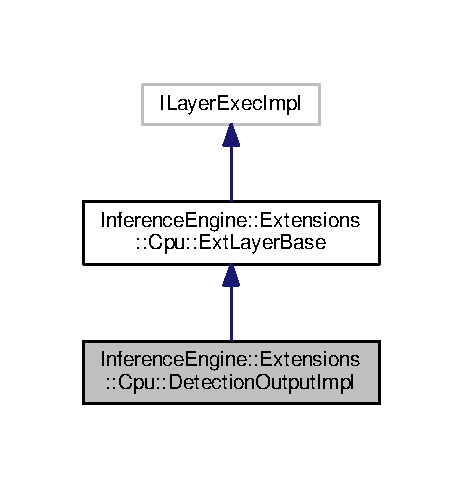
\includegraphics[width=222pt]{classInferenceEngine_1_1Extensions_1_1Cpu_1_1DetectionOutputImpl__inherit__graph}
\end{center}
\end{figure}


Collaboration diagram for Inference\+Engine\+:\+:Extensions\+:\+:Cpu\+:\+:Detection\+Output\+Impl\+:
\nopagebreak
\begin{figure}[H]
\begin{center}
\leavevmode
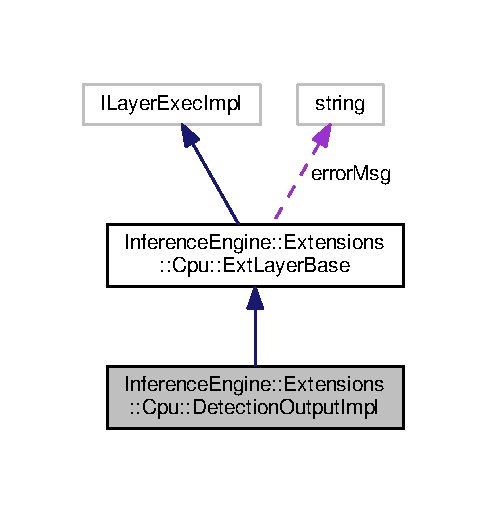
\includegraphics[width=234pt]{classInferenceEngine_1_1Extensions_1_1Cpu_1_1DetectionOutputImpl__coll__graph}
\end{center}
\end{figure}
\subsection*{Public Member Functions}
\begin{DoxyCompactItemize}
\item 
\hyperlink{classInferenceEngine_1_1Extensions_1_1Cpu_1_1DetectionOutputImpl_a65ef73f5900ed006ac1978d7c86f43c8}{Detection\+Output\+Impl} (const C\+N\+N\+Layer $\ast$layer)
\item 
Status\+Code \hyperlink{classInferenceEngine_1_1Extensions_1_1Cpu_1_1DetectionOutputImpl_a4731f24a4a6aec76b0850e12efbd5af3}{execute} (std\+::vector$<$ Blob\+::\+Ptr $>$ \&inputs, std\+::vector$<$ Blob\+::\+Ptr $>$ \&outputs, Response\+Desc $\ast$resp) noexceptoverride
\end{DoxyCompactItemize}
\subsection*{Additional Inherited Members}


\subsection{Detailed Description}


Definition at line 37 of file ext\+\_\+detectionoutput.\+cpp.



\subsection{Constructor \& Destructor Documentation}
\index{Inference\+Engine\+::\+Extensions\+::\+Cpu\+::\+Detection\+Output\+Impl@{Inference\+Engine\+::\+Extensions\+::\+Cpu\+::\+Detection\+Output\+Impl}!Detection\+Output\+Impl@{Detection\+Output\+Impl}}
\index{Detection\+Output\+Impl@{Detection\+Output\+Impl}!Inference\+Engine\+::\+Extensions\+::\+Cpu\+::\+Detection\+Output\+Impl@{Inference\+Engine\+::\+Extensions\+::\+Cpu\+::\+Detection\+Output\+Impl}}
\subsubsection[{\texorpdfstring{Detection\+Output\+Impl(const C\+N\+N\+Layer $\ast$layer)}{DetectionOutputImpl(const CNNLayer *layer)}}]{\setlength{\rightskip}{0pt plus 5cm}Inference\+Engine\+::\+Extensions\+::\+Cpu\+::\+Detection\+Output\+Impl\+::\+Detection\+Output\+Impl (
\begin{DoxyParamCaption}
\item[{const C\+N\+N\+Layer $\ast$}]{layer}
\end{DoxyParamCaption}
)\hspace{0.3cm}{\ttfamily [inline]}, {\ttfamily [explicit]}}\hypertarget{classInferenceEngine_1_1Extensions_1_1Cpu_1_1DetectionOutputImpl_a65ef73f5900ed006ac1978d7c86f43c8}{}\label{classInferenceEngine_1_1Extensions_1_1Cpu_1_1DetectionOutputImpl_a65ef73f5900ed006ac1978d7c86f43c8}


Definition at line 39 of file ext\+\_\+detectionoutput.\+cpp.


\begin{DoxyCode}
39                                                         : \hyperlink{classInferenceEngine_1_1Extensions_1_1Cpu_1_1ExtLayerBase_affff0e8263ca26852ccf71d299d7b06a}{ExtLayerBase}(layer) \{
40         \textcolor{keywordflow}{try} \{
41             \textcolor{keywordflow}{if} (\hyperlink{classInferenceEngine_1_1Extensions_1_1Cpu_1_1ExtLayerBase_a1074cdccacb9e9ca6eec01bbc2f7ca4a}{cnnLayer}.insData.size() != 3)
42                 THROW\_IE\_EXCEPTION << \textcolor{stringliteral}{"Incorrect number of input edges."};
43             \textcolor{keywordflow}{if} (\hyperlink{classInferenceEngine_1_1Extensions_1_1Cpu_1_1ExtLayerBase_a1074cdccacb9e9ca6eec01bbc2f7ca4a}{cnnLayer}.outData.empty())
44                 THROW\_IE\_EXCEPTION << \textcolor{stringliteral}{"Incorrect number of output edges."};
45 
46             \_num\_classes = \hyperlink{classInferenceEngine_1_1Extensions_1_1Cpu_1_1ExtLayerBase_a1074cdccacb9e9ca6eec01bbc2f7ca4a}{cnnLayer}.GetParamAsInt(\textcolor{stringliteral}{"num\_classes"});
47             \_background\_label\_id = \hyperlink{classInferenceEngine_1_1Extensions_1_1Cpu_1_1ExtLayerBase_a1074cdccacb9e9ca6eec01bbc2f7ca4a}{cnnLayer}.GetParamAsInt(\textcolor{stringliteral}{"background\_label\_id"}, 0);
48             \_top\_k = \hyperlink{classInferenceEngine_1_1Extensions_1_1Cpu_1_1ExtLayerBase_a1074cdccacb9e9ca6eec01bbc2f7ca4a}{cnnLayer}.GetParamAsInt(\textcolor{stringliteral}{"top\_k"}, -1);
49             \_variance\_encoded\_in\_target = \hyperlink{classInferenceEngine_1_1Extensions_1_1Cpu_1_1ExtLayerBase_a1074cdccacb9e9ca6eec01bbc2f7ca4a}{cnnLayer}.GetParamsAsBool(\textcolor{stringliteral}{"variance\_encoded\_in\_target"}, \textcolor{keyword}{
      false});
50             \_keep\_top\_k = \hyperlink{classInferenceEngine_1_1Extensions_1_1Cpu_1_1ExtLayerBase_a1074cdccacb9e9ca6eec01bbc2f7ca4a}{cnnLayer}.GetParamAsInt(\textcolor{stringliteral}{"keep\_top\_k"}, -1);
51             \_nms\_threshold = \hyperlink{classInferenceEngine_1_1Extensions_1_1Cpu_1_1ExtLayerBase_a1074cdccacb9e9ca6eec01bbc2f7ca4a}{cnnLayer}.GetParamAsFloat(\textcolor{stringliteral}{"nms\_threshold"});
52             \_confidence\_threshold = \hyperlink{classInferenceEngine_1_1Extensions_1_1Cpu_1_1ExtLayerBase_a1074cdccacb9e9ca6eec01bbc2f7ca4a}{cnnLayer}.GetParamAsFloat(\textcolor{stringliteral}{"confidence\_threshold"}, -FLT\_MAX);
53             \_share\_location = \hyperlink{classInferenceEngine_1_1Extensions_1_1Cpu_1_1ExtLayerBase_a1074cdccacb9e9ca6eec01bbc2f7ca4a}{cnnLayer}.GetParamsAsBool(\textcolor{stringliteral}{"share\_location"}, \textcolor{keyword}{true});
54             \_normalized = \hyperlink{classInferenceEngine_1_1Extensions_1_1Cpu_1_1ExtLayerBase_a1074cdccacb9e9ca6eec01bbc2f7ca4a}{cnnLayer}.GetParamsAsBool(\textcolor{stringliteral}{"normalized"}, \textcolor{keyword}{true});
55             \_image\_height = \hyperlink{classInferenceEngine_1_1Extensions_1_1Cpu_1_1ExtLayerBase_a1074cdccacb9e9ca6eec01bbc2f7ca4a}{cnnLayer}.GetParamAsInt(\textcolor{stringliteral}{"input\_height"}, 1);
56             \_image\_width = \hyperlink{classInferenceEngine_1_1Extensions_1_1Cpu_1_1ExtLayerBase_a1074cdccacb9e9ca6eec01bbc2f7ca4a}{cnnLayer}.GetParamAsInt(\textcolor{stringliteral}{"input\_width"}, 1);
57             \_prior\_size = \_normalized ? 4 : 5;
58             \_offset = \_normalized ? 0 : 1;
59             \_num\_loc\_classes = \_share\_location ? 1 : \_num\_classes;
60 
61             std::string code\_type\_str = \hyperlink{classInferenceEngine_1_1Extensions_1_1Cpu_1_1ExtLayerBase_a1074cdccacb9e9ca6eec01bbc2f7ca4a}{cnnLayer}.GetParamAsString(\textcolor{stringliteral}{"code\_type"}, \textcolor{stringliteral}{"
      caffe.PriorBoxParameter.CORNER"});
62             \_code\_type = (code\_type\_str == \textcolor{stringliteral}{"caffe.PriorBoxParameter.CENTER\_SIZE"} ? CodeType::CENTER\_SIZE
63                                                                                  : CodeType::CORNER);
64 
65             \_num\_priors = \textcolor{keyword}{static\_cast<}\textcolor{keywordtype}{int}\textcolor{keyword}{>}(\hyperlink{classInferenceEngine_1_1Extensions_1_1Cpu_1_1ExtLayerBase_a1074cdccacb9e9ca6eec01bbc2f7ca4a}{cnnLayer}.insData[idx\_priors].lock()->dims[0] / 
      \_prior\_size);
66 
67             \textcolor{keywordflow}{if} (\_num\_priors * \_num\_loc\_classes * 4 != \hyperlink{classInferenceEngine_1_1Extensions_1_1Cpu_1_1ExtLayerBase_a1074cdccacb9e9ca6eec01bbc2f7ca4a}{cnnLayer}.insData[idx\_location].lock()->dims[0
      ])
68                 THROW\_IE\_EXCEPTION << \textcolor{stringliteral}{"Number of priors must match number of location predictions."};
69 
70             \textcolor{keywordflow}{if} (\_num\_priors * \_num\_classes != \hyperlink{classInferenceEngine_1_1Extensions_1_1Cpu_1_1ExtLayerBase_a1074cdccacb9e9ca6eec01bbc2f7ca4a}{cnnLayer}.insData[idx\_confidence].lock()->dims[0])
71                 THROW\_IE\_EXCEPTION << \textcolor{stringliteral}{"Number of priors must match number of confidence predictions."};
72 
73             \textcolor{keywordflow}{if} (\_decrease\_label\_id && \_background\_label\_id != 0)
74                 THROW\_IE\_EXCEPTION << \textcolor{stringliteral}{"Cannot use decrease\_label\_id and background\_label\_id parameter
       simultaneously."};
75 
76             \_num = \textcolor{keyword}{static\_cast<}\textcolor{keywordtype}{int}\textcolor{keyword}{>}(\hyperlink{classInferenceEngine_1_1Extensions_1_1Cpu_1_1ExtLayerBase_a1074cdccacb9e9ca6eec01bbc2f7ca4a}{cnnLayer}.insData[idx\_confidence].lock()->getTensorDesc().
      getDims()[0]);
77 
78             InferenceEngine::SizeVector bboxes\_size\{\textcolor{keyword}{static\_cast<}\textcolor{keywordtype}{size\_t}\textcolor{keyword}{>}(\_num),
79                                                     static\_cast<size\_t>(\_num\_classes),
80                                                     \textcolor{keyword}{static\_cast<}\textcolor{keywordtype}{size\_t}\textcolor{keyword}{>}(\_num\_priors),
81                                                     4\};
82             \_decoded\_bboxes = InferenceEngine::make\_shared\_blob<float>(\{Precision::UNSPECIFIED, bboxes\_size
      , NCHW\});
83             \_decoded\_bboxes->allocate();
84 
85             InferenceEngine::SizeVector buf\_size\{\textcolor{keyword}{static\_cast<}\textcolor{keywordtype}{size\_t}\textcolor{keyword}{>}(\_num),
86                                                  static\_cast<size\_t>(\_num\_classes),
87                                                  \textcolor{keyword}{static\_cast<}\textcolor{keywordtype}{size\_t}\textcolor{keyword}{>}(\_num\_priors)\};
88             \_buffer = InferenceEngine::make\_shared\_blob<int>(\{Precision::UNSPECIFIED, buf\_size, \{buf\_size, 
      \{0, 1, 2\}\}\});
89             \_buffer->allocate();
90 
91             InferenceEngine::SizeVector indices\_size\{\textcolor{keyword}{static\_cast<}\textcolor{keywordtype}{size\_t}\textcolor{keyword}{>}(\_num),
92                                                      static\_cast<size\_t>(\_num\_classes),
93                                                      \textcolor{keyword}{static\_cast<}\textcolor{keywordtype}{size\_t}\textcolor{keyword}{>}(\_num\_priors)\};
94             \_indices = InferenceEngine::make\_shared\_blob<int>(
95                     \{Precision::UNSPECIFIED, indices\_size, \{indices\_size, \{0, 1, 2\}\}\});
96             \_indices->allocate();
97 
98             InferenceEngine::SizeVector detections\_size\{\textcolor{keyword}{static\_cast<}\textcolor{keywordtype}{size\_t}\textcolor{keyword}{>}(\_num * \_num\_classes)\};
99             \_detections\_count = InferenceEngine::make\_shared\_blob<int>(\{Precision::UNSPECIFIED, 
      detections\_size, C\});
100             \_detections\_count->allocate();
101 
102             InferenceEngine::SizeVector conf\_size = \hyperlink{classInferenceEngine_1_1Extensions_1_1Cpu_1_1ExtLayerBase_a1074cdccacb9e9ca6eec01bbc2f7ca4a}{cnnLayer}.insData[idx\_confidence].lock()->dims;
103             \_reordered\_conf = InferenceEngine::make\_shared\_blob<float>(\{Precision::FP32, conf\_size, ANY\});
104             \_reordered\_conf->allocate();
105 
106             InferenceEngine::SizeVector decoded\_bboxes\_size\{\textcolor{keyword}{static\_cast<}\textcolor{keywordtype}{size\_t}\textcolor{keyword}{>}(\_num),
107                                                             static\_cast<size\_t>(\_num\_priors),
108                                                             \textcolor{keyword}{static\_cast<}\textcolor{keywordtype}{size\_t}\textcolor{keyword}{>}(\_num\_classes)\};
109             \_bbox\_sizes = InferenceEngine::make\_shared\_blob<float>(
110                     \{Precision::FP32, decoded\_bboxes\_size, \{decoded\_bboxes\_size, \{0, 1, 2\}\}\});
111             \_bbox\_sizes->allocate();
112 
113             InferenceEngine::SizeVector num\_priors\_actual\_size\{\textcolor{keyword}{static\_cast<}\textcolor{keywordtype}{size\_t}\textcolor{keyword}{>}(\_num)\};
114             \_num\_priors\_actual = InferenceEngine::make\_shared\_blob<int>(\{Precision::UNSPECIFIED, 
      num\_priors\_actual\_size, C\});
115             \_num\_priors\_actual->allocate();
116 
117             \hyperlink{classInferenceEngine_1_1Extensions_1_1Cpu_1_1ExtLayerBase_a0ac7a6632e95b9500d5246b05b4b0bfa}{addConfig}(\{DataConfigurator(\hyperlink{classInferenceEngine_1_1Extensions_1_1Cpu_1_1ExtLayerBase_a1258a8d209e0249e0b1717618352ddfba446687ea2db1ada75be5ed053be77f59}{ConfLayout::PLN}),
118                        DataConfigurator(\hyperlink{classInferenceEngine_1_1Extensions_1_1Cpu_1_1ExtLayerBase_a1258a8d209e0249e0b1717618352ddfba446687ea2db1ada75be5ed053be77f59}{ConfLayout::PLN}),
119                        DataConfigurator(\hyperlink{classInferenceEngine_1_1Extensions_1_1Cpu_1_1ExtLayerBase_a1258a8d209e0249e0b1717618352ddfba446687ea2db1ada75be5ed053be77f59}{ConfLayout::PLN})\}, \{DataConfigurator(
      \hyperlink{classInferenceEngine_1_1Extensions_1_1Cpu_1_1ExtLayerBase_a1258a8d209e0249e0b1717618352ddfba446687ea2db1ada75be5ed053be77f59}{ConfLayout::PLN})\});
120         \} \textcolor{keywordflow}{catch} (InferenceEngine::details::InferenceEngineException &ex) \{
121             \hyperlink{classInferenceEngine_1_1Extensions_1_1Cpu_1_1ExtLayerBase_abc78e9b5a79fa339ffd831a5318f71f7}{errorMsg} = ex.what();
122         \}
123     \}
\end{DoxyCode}


\subsection{Member Function Documentation}
\index{Inference\+Engine\+::\+Extensions\+::\+Cpu\+::\+Detection\+Output\+Impl@{Inference\+Engine\+::\+Extensions\+::\+Cpu\+::\+Detection\+Output\+Impl}!execute@{execute}}
\index{execute@{execute}!Inference\+Engine\+::\+Extensions\+::\+Cpu\+::\+Detection\+Output\+Impl@{Inference\+Engine\+::\+Extensions\+::\+Cpu\+::\+Detection\+Output\+Impl}}
\subsubsection[{\texorpdfstring{execute(std\+::vector$<$ Blob\+::\+Ptr $>$ \&inputs, std\+::vector$<$ Blob\+::\+Ptr $>$ \&outputs, Response\+Desc $\ast$resp) noexceptoverride}{execute(std::vector< Blob::Ptr > &inputs, std::vector< Blob::Ptr > &outputs, ResponseDesc *resp) noexceptoverride}}]{\setlength{\rightskip}{0pt plus 5cm}Status\+Code Inference\+Engine\+::\+Extensions\+::\+Cpu\+::\+Detection\+Output\+Impl\+::execute (
\begin{DoxyParamCaption}
\item[{std\+::vector$<$ Blob\+::\+Ptr $>$ \&}]{inputs, }
\item[{std\+::vector$<$ Blob\+::\+Ptr $>$ \&}]{outputs, }
\item[{Response\+Desc $\ast$}]{resp}
\end{DoxyParamCaption}
)\hspace{0.3cm}{\ttfamily [inline]}, {\ttfamily [override]}, {\ttfamily [noexcept]}}\hypertarget{classInferenceEngine_1_1Extensions_1_1Cpu_1_1DetectionOutputImpl_a4731f24a4a6aec76b0850e12efbd5af3}{}\label{classInferenceEngine_1_1Extensions_1_1Cpu_1_1DetectionOutputImpl_a4731f24a4a6aec76b0850e12efbd5af3}


Definition at line 125 of file ext\+\_\+detectionoutput.\+cpp.


\begin{DoxyCode}
126                                                              \{
127         \textcolor{keywordtype}{float} *dst\_data = outputs[0]->buffer();
128 
129         \textcolor{keyword}{const} \textcolor{keywordtype}{float} *loc\_data    = inputs[idx\_location]->buffer();
130         \textcolor{keyword}{const} \textcolor{keywordtype}{float} *conf\_data   = inputs[idx\_confidence]->buffer();
131         \textcolor{keyword}{const} \textcolor{keywordtype}{float} *prior\_data  = inputs[idx\_priors]->buffer();
132 
133         \textcolor{keyword}{const} \textcolor{keywordtype}{int} N = inputs[idx\_confidence]->getTensorDesc().getDims()[0];
134 
135         \textcolor{keywordtype}{float} *decoded\_bboxes\_data = \_decoded\_bboxes->buffer();
136         \textcolor{keywordtype}{float} *reordered\_conf\_data = \_reordered\_conf->buffer();
137         \textcolor{keywordtype}{float} *bbox\_sizes\_data     = \_bbox\_sizes->buffer();
138         \textcolor{keywordtype}{int} *detections\_data       = \_detections\_count->buffer();
139         \textcolor{keywordtype}{int} *buffer\_data           = \_buffer->buffer();
140         \textcolor{keywordtype}{int} *indices\_data          = \_indices->buffer();
141         \textcolor{keywordtype}{int} *num\_priors\_actual     = \_num\_priors\_actual->buffer();
142 
143         \textcolor{keyword}{const} \textcolor{keywordtype}{float} *prior\_variances = prior\_data + \_num\_priors*\_prior\_size;
144         \textcolor{keyword}{const} \textcolor{keywordtype}{float} *ppriors = prior\_data;
145 
146         \textcolor{keywordflow}{for} (\textcolor{keywordtype}{int} n = 0; n < N; ++n) \{
147             \textcolor{keywordflow}{if} (\_share\_location) \{
148                 \textcolor{keyword}{const} \textcolor{keywordtype}{float} *ploc = loc\_data + n*4*\_num\_priors;
149                 \textcolor{keywordtype}{float} *pboxes = decoded\_bboxes\_data + n*4*\_num\_priors;
150                 \textcolor{keywordtype}{float} *psizes = bbox\_sizes\_data + n*\_num\_priors;
151                 decodeBBoxes(ppriors, ploc, prior\_variances, pboxes, psizes, num\_priors\_actual, n);
152             \} \textcolor{keywordflow}{else} \{
153                 \textcolor{keywordflow}{for} (\textcolor{keywordtype}{int} \hyperlink{CMakeCache_8txt_aac1d6a1710812201527c735f7c6afbaa}{c} = 0; \hyperlink{CMakeCache_8txt_aac1d6a1710812201527c735f7c6afbaa}{c} < \_num\_loc\_classes; ++\hyperlink{CMakeCache_8txt_aac1d6a1710812201527c735f7c6afbaa}{c}) \{
154                     \textcolor{keywordflow}{if} (\hyperlink{CMakeCache_8txt_aac1d6a1710812201527c735f7c6afbaa}{c} == \_background\_label\_id) \{
155                         \textcolor{keywordflow}{continue};
156                     \}
157 
158                     \textcolor{keyword}{const} \textcolor{keywordtype}{float} *ploc = loc\_data + n*4*\_num\_loc\_classes*\_num\_priors + 
      \hyperlink{CMakeCache_8txt_aac1d6a1710812201527c735f7c6afbaa}{c}*4;
159                     \textcolor{keywordtype}{float} *pboxes = decoded\_bboxes\_data + n*4*\_num\_loc\_classes*\_num\_priors + c*4*
      \_num\_priors;
160                     \textcolor{keywordtype}{float} *psizes = bbox\_sizes\_data + n*\_num\_loc\_classes*\_num\_priors + c*\_num\_priors;
161                     decodeBBoxes(ppriors, ploc, prior\_variances, pboxes, psizes, num\_priors\_actual, n);
162                 \}
163             \}
164         \}
165 
166         \textcolor{keywordflow}{for} (\textcolor{keywordtype}{int} n = 0; n < N; ++n) \{
167             \textcolor{keywordflow}{for} (\textcolor{keywordtype}{int} \hyperlink{CMakeCache_8txt_aac1d6a1710812201527c735f7c6afbaa}{c} = 0; \hyperlink{CMakeCache_8txt_aac1d6a1710812201527c735f7c6afbaa}{c} < \_num\_classes; ++\hyperlink{CMakeCache_8txt_aac1d6a1710812201527c735f7c6afbaa}{c}) \{
168                 \textcolor{keywordflow}{for} (\textcolor{keywordtype}{int} p = 0; p < \_num\_priors; ++p) \{
169                     reordered\_conf\_data[n*\_num\_priors*\_num\_classes + \hyperlink{CMakeCache_8txt_aac1d6a1710812201527c735f7c6afbaa}{c}*\_num\_priors + p] = conf\_data[n*
      \_num\_priors*\_num\_classes + p*\_num\_classes + \hyperlink{CMakeCache_8txt_aac1d6a1710812201527c735f7c6afbaa}{c}];
170                 \}
171             \}
172         \}
173 
174         memset(detections\_data, 0, N*\_num\_classes*\textcolor{keyword}{sizeof}(\textcolor{keywordtype}{int}));
175 
176         \textcolor{keywordflow}{for} (\textcolor{keywordtype}{int} n = 0; n < N; ++n) \{
177             \textcolor{keywordtype}{int} detections\_total = 0;
178 
179 \textcolor{preprocessor}{#pragma omp parallel for schedule(static)}
180             \textcolor{keywordflow}{for} (\textcolor{keywordtype}{int} \hyperlink{CMakeCache_8txt_aac1d6a1710812201527c735f7c6afbaa}{c} = 0; \hyperlink{CMakeCache_8txt_aac1d6a1710812201527c735f7c6afbaa}{c} < \_num\_classes; ++\hyperlink{CMakeCache_8txt_aac1d6a1710812201527c735f7c6afbaa}{c}) \{
181                 \textcolor{keywordflow}{if} (\hyperlink{CMakeCache_8txt_aac1d6a1710812201527c735f7c6afbaa}{c} == \_background\_label\_id) \{
182                     \textcolor{comment}{// Ignore background class.}
183                     \textcolor{keywordflow}{continue};
184                 \}
185 
186                 \textcolor{keywordtype}{int} *pindices    = indices\_data + n*\_num\_classes*\_num\_priors + \hyperlink{CMakeCache_8txt_aac1d6a1710812201527c735f7c6afbaa}{c}*\_num\_priors;
187                 \textcolor{keywordtype}{int} *pbuffer     = buffer\_data + \hyperlink{CMakeCache_8txt_aac1d6a1710812201527c735f7c6afbaa}{c}*\_num\_priors;
188                 \textcolor{keywordtype}{int} *pdetections = detections\_data + n*\_num\_classes + \hyperlink{CMakeCache_8txt_aac1d6a1710812201527c735f7c6afbaa}{c};
189 
190                 \textcolor{keyword}{const} \textcolor{keywordtype}{float} *pconf = reordered\_conf\_data + n*\_num\_classes*\_num\_priors + c*\_num\_priors;
191                 \textcolor{keyword}{const} \textcolor{keywordtype}{float} *pboxes;
192                 \textcolor{keyword}{const} \textcolor{keywordtype}{float} *psizes;
193                 \textcolor{keywordflow}{if} (\_share\_location) \{
194                     pboxes = decoded\_bboxes\_data + n*4*\_num\_priors;
195                     psizes = bbox\_sizes\_data + n*\_num\_priors;
196                 \} \textcolor{keywordflow}{else} \{
197                     pboxes = decoded\_bboxes\_data + n*4*\_num\_classes*\_num\_priors + c*4*\_num\_priors;
198                     psizes = bbox\_sizes\_data + n*\_num\_classes*\_num\_priors + c*\_num\_priors;
199                 \}
200 
201                 nms(pconf, pboxes, psizes, pbuffer, pindices, *pdetections, num\_priors\_actual[n]);
202             \}
203 
204             \textcolor{keywordflow}{for} (\textcolor{keywordtype}{int} c = 0; c < \_num\_classes; ++\hyperlink{CMakeCache_8txt_aac1d6a1710812201527c735f7c6afbaa}{c}) \{
205                 detections\_total += detections\_data[n*\_num\_classes + \hyperlink{CMakeCache_8txt_aac1d6a1710812201527c735f7c6afbaa}{c}];
206             \}
207 
208             \textcolor{keywordflow}{if} (\_keep\_top\_k > -1 && detections\_total > \_keep\_top\_k) \{
209                 std::vector<std::pair<float, std::pair<int, int>>> conf\_index\_class\_map;
210 
211                 \textcolor{keywordflow}{for} (\textcolor{keywordtype}{int} c = 0; c < \_num\_classes; ++\hyperlink{CMakeCache_8txt_aac1d6a1710812201527c735f7c6afbaa}{c}) \{
212                     \textcolor{keywordtype}{int} detections = detections\_data[n*\_num\_classes + \hyperlink{CMakeCache_8txt_aac1d6a1710812201527c735f7c6afbaa}{c}];
213                     \textcolor{keywordtype}{int} *pindices = indices\_data + n*\_num\_classes*\_num\_priors + c*\_num\_priors;
214                     \textcolor{keywordtype}{float} *pconf  = reordered\_conf\_data + n*\_num\_classes*\_num\_priors + c*\_num\_priors;
215 
216                     \textcolor{keywordflow}{for} (\textcolor{keywordtype}{int} i = 0; i < detections; ++i) \{
217                         \textcolor{keywordtype}{int} idx = pindices[i];
218                         conf\_index\_class\_map.push\_back(std::make\_pair(pconf[idx], std::make\_pair(c, idx)));
219                     \}
220                 \}
221 
222                 std::sort(conf\_index\_class\_map.begin(), conf\_index\_class\_map.end(),
223                           SortScorePairDescend<std::pair<int, int>>);
224                 conf\_index\_class\_map.resize(\_keep\_top\_k);
225 
226                 \textcolor{comment}{// Store the new indices.}
227                 memset(detections\_data + n*\_num\_classes, 0, \_num\_classes * \textcolor{keyword}{sizeof}(\textcolor{keywordtype}{int}));
228 
229                 \textcolor{keywordflow}{for} (\textcolor{keywordtype}{int} j = 0; j < conf\_index\_class\_map.size(); ++j) \{
230                     \textcolor{keywordtype}{int} label = conf\_index\_class\_map[j].second.first;
231                     \textcolor{keywordtype}{int} idx = conf\_index\_class\_map[j].second.second;
232                     \textcolor{keywordtype}{int} *pindices = indices\_data + n * \_num\_classes * \_num\_priors + label * \_num\_priors;
233                     pindices[detections\_data[n*\_num\_classes + label]] = idx;
234                     detections\_data[n*\_num\_classes + label]++;
235                 \}
236             \}
237         \}
238 
239         \textcolor{keyword}{const} \textcolor{keywordtype}{int} DETECTION\_SIZE = outputs[0]->getTensorDesc().getDims()[3];
240         \textcolor{keywordflow}{if} (DETECTION\_SIZE != 7) \{
241             \textcolor{keywordflow}{return} NOT\_IMPLEMENTED;
242         \}
243 
244         \textcolor{keyword}{auto} dst\_data\_size = N * \_keep\_top\_k * DETECTION\_SIZE * \textcolor{keyword}{sizeof}(float);
245 
246         \textcolor{keywordflow}{if} (dst\_data\_size > outputs[0]->byteSize()) \{
247             \textcolor{keywordflow}{return} OUT\_OF\_BOUNDS;
248         \}
249 
250         memset(dst\_data, 0, dst\_data\_size);
251 
252         \textcolor{keywordtype}{int} count = 0;
253         \textcolor{keywordflow}{for} (\textcolor{keywordtype}{int} n = 0; n < N; ++n) \{
254             \textcolor{keyword}{const} \textcolor{keywordtype}{float} *pconf   = reordered\_conf\_data + n * \_num\_priors * \_num\_classes;
255             \textcolor{keyword}{const} \textcolor{keywordtype}{float} *pboxes  = decoded\_bboxes\_data + n*\_num\_priors*4*\_num\_loc\_classes;
256             \textcolor{keyword}{const} \textcolor{keywordtype}{int} *pindices  = indices\_data + n*\_num\_classes*\_num\_priors;
257 
258             \textcolor{keywordflow}{for} (\textcolor{keywordtype}{int} c = 0; c < \_num\_classes; ++\hyperlink{CMakeCache_8txt_aac1d6a1710812201527c735f7c6afbaa}{c}) \{
259                 \textcolor{keywordflow}{for} (\textcolor{keywordtype}{int} i = 0; i < detections\_data[n*\_num\_classes + \hyperlink{CMakeCache_8txt_aac1d6a1710812201527c735f7c6afbaa}{c}]; ++i) \{
260                     \textcolor{keywordtype}{int} idx = pindices[c*\_num\_priors + i];
261 
262                     dst\_data[count * DETECTION\_SIZE + 0] = n;
263                     dst\_data[count * DETECTION\_SIZE + 1] = \_decrease\_label\_id ? c-1 : 
      \hyperlink{CMakeCache_8txt_aac1d6a1710812201527c735f7c6afbaa}{c};
264                     dst\_data[count * DETECTION\_SIZE + 2] = pconf[c*\_num\_priors + idx];
265 
266                     \textcolor{keywordtype}{float} xmin = \_share\_location ? pboxes[idx*4 + 0] :
267                                  pboxes[c*4*\_num\_priors + idx*4 + 0];
268                     \textcolor{keywordtype}{float} ymin = \_share\_location ? pboxes[idx*4 + 1] :
269                                  pboxes[c*4*\_num\_priors + idx*4 + 1];
270                     \textcolor{keywordtype}{float} xmax = \_share\_location ? pboxes[idx*4 + 2] :
271                                  pboxes[c*4*\_num\_priors + idx*4 + 2];
272                     \textcolor{keywordtype}{float} ymax = \_share\_location ? pboxes[idx*4 + 3] :
273                                  pboxes[c*4*\_num\_priors + idx*4 + 3];
274 
275                     dst\_data[count * DETECTION\_SIZE + 3] = xmin;
276                     dst\_data[count * DETECTION\_SIZE + 4] = ymin;
277                     dst\_data[count * DETECTION\_SIZE + 5] = xmax;
278                     dst\_data[count * DETECTION\_SIZE + 6] = ymax;
279 
280                     ++count;
281                 \}
282             \}
283         \}
284 
285         \textcolor{keywordflow}{if} (count < N*\_keep\_top\_k) \{
286             \textcolor{comment}{// marker at end of boxes list}
287             dst\_data[count * DETECTION\_SIZE + 0] = -1;
288         \}
289 
290         \textcolor{keywordflow}{return} OK;
291     \}
\end{DoxyCode}


The documentation for this class was generated from the following file\+:\begin{DoxyCompactItemize}
\item 
thirdparty/extension/\hyperlink{ext__detectionoutput_8cpp}{ext\+\_\+detectionoutput.\+cpp}\end{DoxyCompactItemize}

\hypertarget{classDIR}{}\section{D\+IR Class Reference}
\label{classDIR}\index{D\+IR@{D\+IR}}


{\ttfamily \#include $<$w\+\_\+dirent.\+h$>$}

\subsection*{Public Member Functions}
\begin{DoxyCompactItemize}
\item 
\hyperlink{classDIR_aaaf220338866159ad97dd91038540bbf}{D\+IR} (const \hyperlink{CMakeCache_8txt_afe71f11dacb15682cdc012f7208e6e09}{char} $\ast$dir\+Path)
\item 
\hyperlink{classDIR_af4e768b5794043041e674cdc1458ccc7}{$\sim$\+D\+IR} ()
\item 
bool \hyperlink{classDIR_a2dfa4e833f3b4143772a6c6cfbac9543}{is\+Valid} () const 
\item 
\hyperlink{structdirent}{dirent} $\ast$ \hyperlink{classDIR_a4d773fa1ff4d74396da57cfed3fe1aef}{next\+Ent} ()
\end{DoxyCompactItemize}


\subsection{Detailed Description}


Definition at line 57 of file w\+\_\+dirent.\+h.



\subsection{Constructor \& Destructor Documentation}
\index{D\+IR@{D\+IR}!D\+IR@{D\+IR}}
\index{D\+IR@{D\+IR}!D\+IR@{D\+IR}}
\subsubsection[{\texorpdfstring{D\+I\+R(const char $\ast$dir\+Path)}{DIR(const char *dirPath)}}]{\setlength{\rightskip}{0pt plus 5cm}D\+I\+R\+::\+D\+IR (
\begin{DoxyParamCaption}
\item[{const {\bf char} $\ast$}]{dir\+Path}
\end{DoxyParamCaption}
)\hspace{0.3cm}{\ttfamily [inline]}, {\ttfamily [explicit]}}\hypertarget{classDIR_aaaf220338866159ad97dd91038540bbf}{}\label{classDIR_aaaf220338866159ad97dd91038540bbf}


Definition at line 70 of file w\+\_\+dirent.\+h.


\begin{DoxyCode}
70                                       : next(\textcolor{keyword}{nullptr}) \{
71         std::string ws = dirPath;
72         \textcolor{keywordflow}{if} (endsWith(ws, \textcolor{stringliteral}{"\(\backslash\)\(\backslash\)"}))
73             ws += \textcolor{stringliteral}{"*"};
74         \textcolor{keywordflow}{else}
75             ws += \textcolor{stringliteral}{"\(\backslash\)\(\backslash\)*"};
76         hFind = FindFirstFile(ws.c\_str(), &FindFileData);
77         FindFileData.dwReserved0 = hFind != INVALID\_HANDLE\_VALUE;
78     \}
\end{DoxyCode}
\index{D\+IR@{D\+IR}!````~D\+IR@{$\sim$\+D\+IR}}
\index{````~D\+IR@{$\sim$\+D\+IR}!D\+IR@{D\+IR}}
\subsubsection[{\texorpdfstring{$\sim$\+D\+I\+R()}{~DIR()}}]{\setlength{\rightskip}{0pt plus 5cm}D\+I\+R\+::$\sim$\+D\+IR (
\begin{DoxyParamCaption}
{}
\end{DoxyParamCaption}
)\hspace{0.3cm}{\ttfamily [inline]}}\hypertarget{classDIR_af4e768b5794043041e674cdc1458ccc7}{}\label{classDIR_af4e768b5794043041e674cdc1458ccc7}


Definition at line 80 of file w\+\_\+dirent.\+h.


\begin{DoxyCode}
80            \{
81         \textcolor{keywordflow}{if} (!next) \textcolor{keyword}{delete} next;
82         FindClose(hFind);
83     \}
\end{DoxyCode}


\subsection{Member Function Documentation}
\index{D\+IR@{D\+IR}!is\+Valid@{is\+Valid}}
\index{is\+Valid@{is\+Valid}!D\+IR@{D\+IR}}
\subsubsection[{\texorpdfstring{is\+Valid() const }{isValid() const }}]{\setlength{\rightskip}{0pt plus 5cm}bool D\+I\+R\+::is\+Valid (
\begin{DoxyParamCaption}
{}
\end{DoxyParamCaption}
) const\hspace{0.3cm}{\ttfamily [inline]}}\hypertarget{classDIR_a2dfa4e833f3b4143772a6c6cfbac9543}{}\label{classDIR_a2dfa4e833f3b4143772a6c6cfbac9543}


Definition at line 85 of file w\+\_\+dirent.\+h.


\begin{DoxyCode}
85                          \{
86         \textcolor{keywordflow}{return} (hFind != INVALID\_HANDLE\_VALUE && FindFileData.dwReserved0);
87     \}
\end{DoxyCode}
\index{D\+IR@{D\+IR}!next\+Ent@{next\+Ent}}
\index{next\+Ent@{next\+Ent}!D\+IR@{D\+IR}}
\subsubsection[{\texorpdfstring{next\+Ent()}{nextEnt()}}]{\setlength{\rightskip}{0pt plus 5cm}{\bf dirent}$\ast$ D\+I\+R\+::next\+Ent (
\begin{DoxyParamCaption}
{}
\end{DoxyParamCaption}
)\hspace{0.3cm}{\ttfamily [inline]}}\hypertarget{classDIR_a4d773fa1ff4d74396da57cfed3fe1aef}{}\label{classDIR_a4d773fa1ff4d74396da57cfed3fe1aef}


Definition at line 89 of file w\+\_\+dirent.\+h.


\begin{DoxyCode}
89                       \{
90         \textcolor{keywordflow}{if} (next != \textcolor{keyword}{nullptr}) \textcolor{keyword}{delete} next;
91         next = \textcolor{keyword}{nullptr};
92 
93         \textcolor{keywordflow}{if} (!FindFileData.dwReserved0) \textcolor{keywordflow}{return} \textcolor{keyword}{nullptr};
94 
95         \textcolor{keywordtype}{wchar\_t} wbuf[4096];
96 
97         \textcolor{keywordtype}{size\_t} outSize;
98         mbstowcs\_s(&outSize, wbuf, 4094, FindFileData.cFileName, 4094);
99         next = \textcolor{keyword}{new} \hyperlink{structdirent}{dirent}(wbuf);
100         FindFileData.dwReserved0 = FindNextFile(hFind, &FindFileData);
101         \textcolor{keywordflow}{return} next;
102     \}
\end{DoxyCode}


The documentation for this class was generated from the following file\+:\begin{DoxyCompactItemize}
\item 
thirdparty/common/os/windows/\hyperlink{w__dirent_8h}{w\+\_\+dirent.\+h}\end{DoxyCompactItemize}

\hypertarget{structdirent}{}\section{dirent Struct Reference}
\label{structdirent}\index{dirent@{dirent}}


{\ttfamily \#include $<$w\+\_\+dirent.\+h$>$}

\subsection*{Public Member Functions}
\begin{DoxyCompactItemize}
\item 
\hyperlink{structdirent_a8e402a3698700524bcf424dbc220c81d}{dirent} (const wchar\+\_\+t $\ast$ws\+File\+Path)
\item 
\hyperlink{structdirent_a14961bb2c1b5fbf6328ed9738afea575}{$\sim$dirent} ()
\end{DoxyCompactItemize}
\subsection*{Public Attributes}
\begin{DoxyCompactItemize}
\item 
\hyperlink{CMakeCache_8txt_afe71f11dacb15682cdc012f7208e6e09}{char} $\ast$ \hyperlink{structdirent_ab703007dd91aa1f311cf0fc85268b2e1}{d\+\_\+name}
\end{DoxyCompactItemize}


\subsection{Detailed Description}


Definition at line 42 of file w\+\_\+dirent.\+h.



\subsection{Constructor \& Destructor Documentation}
\index{dirent@{dirent}!dirent@{dirent}}
\index{dirent@{dirent}!dirent@{dirent}}
\subsubsection[{\texorpdfstring{dirent(const wchar\+\_\+t $\ast$ws\+File\+Path)}{dirent(const wchar_t *wsFilePath)}}]{\setlength{\rightskip}{0pt plus 5cm}dirent\+::dirent (
\begin{DoxyParamCaption}
\item[{const wchar\+\_\+t $\ast$}]{ws\+File\+Path}
\end{DoxyParamCaption}
)\hspace{0.3cm}{\ttfamily [inline]}, {\ttfamily [explicit]}}\hypertarget{structdirent_a8e402a3698700524bcf424dbc220c81d}{}\label{structdirent_a8e402a3698700524bcf424dbc220c81d}


Definition at line 45 of file w\+\_\+dirent.\+h.


\begin{DoxyCode}
45                                                \{
46         \textcolor{keywordtype}{size\_t} i;
47         \textcolor{keyword}{auto} slen = wcslen(wsFilePath);
48         \hyperlink{structdirent_ab703007dd91aa1f311cf0fc85268b2e1}{d\_name} = \textcolor{keyword}{static\_cast<}\textcolor{keywordtype}{char}*\textcolor{keyword}{>}(malloc(slen + 1));
49         wcstombs\_s(&i, \hyperlink{structdirent_ab703007dd91aa1f311cf0fc85268b2e1}{d\_name}, slen + 1, wsFilePath, slen);
50     \}
\end{DoxyCode}
\index{dirent@{dirent}!````~dirent@{$\sim$dirent}}
\index{````~dirent@{$\sim$dirent}!dirent@{dirent}}
\subsubsection[{\texorpdfstring{$\sim$dirent()}{~dirent()}}]{\setlength{\rightskip}{0pt plus 5cm}dirent\+::$\sim$dirent (
\begin{DoxyParamCaption}
{}
\end{DoxyParamCaption}
)\hspace{0.3cm}{\ttfamily [inline]}}\hypertarget{structdirent_a14961bb2c1b5fbf6328ed9738afea575}{}\label{structdirent_a14961bb2c1b5fbf6328ed9738afea575}


Definition at line 52 of file w\+\_\+dirent.\+h.


\begin{DoxyCode}
52               \{
53         free(\hyperlink{structdirent_ab703007dd91aa1f311cf0fc85268b2e1}{d\_name});
54     \}
\end{DoxyCode}


\subsection{Member Data Documentation}
\index{dirent@{dirent}!d\+\_\+name@{d\+\_\+name}}
\index{d\+\_\+name@{d\+\_\+name}!dirent@{dirent}}
\subsubsection[{\texorpdfstring{d\+\_\+name}{d_name}}]{\setlength{\rightskip}{0pt plus 5cm}{\bf char}$\ast$ dirent\+::d\+\_\+name}\hypertarget{structdirent_ab703007dd91aa1f311cf0fc85268b2e1}{}\label{structdirent_ab703007dd91aa1f311cf0fc85268b2e1}


Definition at line 43 of file w\+\_\+dirent.\+h.



The documentation for this struct was generated from the following file\+:\begin{DoxyCompactItemize}
\item 
thirdparty/common/os/windows/\hyperlink{w__dirent_8h}{w\+\_\+dirent.\+h}\end{DoxyCompactItemize}

\hypertarget{classopenvino__service_1_1EmotionsDetection}{}\section{openvino\+\_\+service\+:\+:Emotions\+Detection Class Reference}
\label{classopenvino__service_1_1EmotionsDetection}\index{openvino\+\_\+service\+::\+Emotions\+Detection@{openvino\+\_\+service\+::\+Emotions\+Detection}}


{\ttfamily \#include $<$emotions\+\_\+recognition.\+h$>$}



Inheritance diagram for openvino\+\_\+service\+:\+:Emotions\+Detection\+:
\nopagebreak
\begin{figure}[H]
\begin{center}
\leavevmode
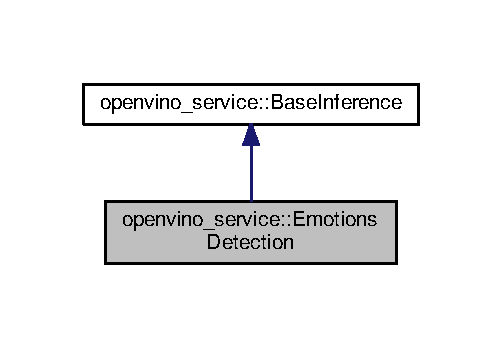
\includegraphics[width=241pt]{classopenvino__service_1_1EmotionsDetection__inherit__graph}
\end{center}
\end{figure}


Collaboration diagram for openvino\+\_\+service\+:\+:Emotions\+Detection\+:
\nopagebreak
\begin{figure}[H]
\begin{center}
\leavevmode
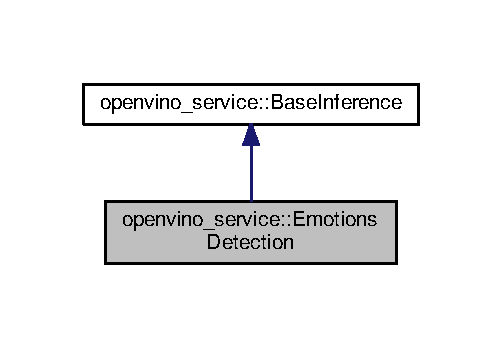
\includegraphics[width=241pt]{classopenvino__service_1_1EmotionsDetection__coll__graph}
\end{center}
\end{figure}
\subsection*{Public Types}
\begin{DoxyCompactItemize}
\item 
using \hyperlink{classopenvino__service_1_1EmotionsDetection_afa51d5786d9296111bda1b928e87afa8}{Result} = \hyperlink{structInferenceResult_1_1EmotionsResult}{Inference\+Result\+::\+Emotions\+Result}
\end{DoxyCompactItemize}
\subsection*{Public Member Functions}
\begin{DoxyCompactItemize}
\item 
\hyperlink{classopenvino__service_1_1EmotionsDetection_af39351c4a6c366007bf523d569855cd9}{Emotions\+Detection} ()
\item 
\hyperlink{classopenvino__service_1_1EmotionsDetection_a7eeb58a704c56aa0f2f73b980cb44ac5}{$\sim$\+Emotions\+Detection} () override
\item 
void \hyperlink{classopenvino__service_1_1EmotionsDetection_af76ffdb8f2a97006b522b13a77488f5e}{load\+Network} (std\+::shared\+\_\+ptr$<$ \hyperlink{classValidatedEmotionsClassificationNetwork}{Validated\+Emotions\+Classification\+Network} $>$)
\item 
bool \hyperlink{classopenvino__service_1_1EmotionsDetection_a170516f06ee4b84f378869b3addc8740}{enqueue} (const cv\+::\+Mat \&, const cv\+::\+Rect \&) override
\begin{DoxyCompactList}\small\item\em Enqueue a frame to this class. The frame will be buffered but not infered yet. \end{DoxyCompactList}\item 
bool \hyperlink{classopenvino__service_1_1EmotionsDetection_ab4a36bef8e7b0af39f7965cf8c5f9d7b}{submit\+Request} () override
\begin{DoxyCompactList}\small\item\em Start inference for all buffered frames. \end{DoxyCompactList}\item 
bool \hyperlink{classopenvino__service_1_1EmotionsDetection_af2af5cf3315347dfbd81008e9987a97c}{fetch\+Results} () override
\begin{DoxyCompactList}\small\item\em This function will fetch the results of the previous inference and stores the results in a result buffer array. All buffered frames will be cleared. \end{DoxyCompactList}\item 
void \hyperlink{classopenvino__service_1_1EmotionsDetection_ad3b3e5f68943041161b02f4c56de763e}{accepts} (std\+::shared\+\_\+ptr$<$ \hyperlink{classBaseOutput}{Base\+Output} $>$ output\+\_\+visitor) override
\begin{DoxyCompactList}\small\item\em Accepts an Output instance for result process. This function is used for visitor pattern. \end{DoxyCompactList}\item 
const \hyperlink{CMakeCache_8txt_a79a3d8790b2588b09777910863574e09}{int} \hyperlink{classopenvino__service_1_1EmotionsDetection_ac240dcf338a9e7b4da78597be5219266}{get\+Results\+Length} () const override
\begin{DoxyCompactList}\small\item\em Get the length of the buffer result array. \end{DoxyCompactList}\item 
const \hyperlink{structInferenceResult_1_1Result}{Inference\+Result\+::\+Result} \hyperlink{classopenvino__service_1_1EmotionsDetection_a4b235a72ba45667a2e8a54ea595ce22c}{get\+Location\+Result} (\hyperlink{CMakeCache_8txt_a79a3d8790b2588b09777910863574e09}{int} idx) const override
\begin{DoxyCompactList}\small\item\em Get the location of result with respect to the frame generated by the input device. \end{DoxyCompactList}\item 
const std\+::string \hyperlink{classopenvino__service_1_1EmotionsDetection_a676e7c587ce0bc41de50f8da60642bd6}{get\+Name} () const override
\begin{DoxyCompactList}\small\item\em Get the name of the Inference instance. \end{DoxyCompactList}\end{DoxyCompactItemize}
\subsection*{Additional Inherited Members}


\subsection{Detailed Description}


Definition at line 20 of file emotions\+\_\+recognition.\+h.



\subsection{Member Typedef Documentation}
\index{openvino\+\_\+service\+::\+Emotions\+Detection@{openvino\+\_\+service\+::\+Emotions\+Detection}!Result@{Result}}
\index{Result@{Result}!openvino\+\_\+service\+::\+Emotions\+Detection@{openvino\+\_\+service\+::\+Emotions\+Detection}}
\subsubsection[{\texorpdfstring{Result}{Result}}]{\setlength{\rightskip}{0pt plus 5cm}using {\bf openvino\+\_\+service\+::\+Emotions\+Detection\+::\+Result} =  {\bf Inference\+Result\+::\+Emotions\+Result}}\hypertarget{classopenvino__service_1_1EmotionsDetection_afa51d5786d9296111bda1b928e87afa8}{}\label{classopenvino__service_1_1EmotionsDetection_afa51d5786d9296111bda1b928e87afa8}


Definition at line 22 of file emotions\+\_\+recognition.\+h.



\subsection{Constructor \& Destructor Documentation}
\index{openvino\+\_\+service\+::\+Emotions\+Detection@{openvino\+\_\+service\+::\+Emotions\+Detection}!Emotions\+Detection@{Emotions\+Detection}}
\index{Emotions\+Detection@{Emotions\+Detection}!openvino\+\_\+service\+::\+Emotions\+Detection@{openvino\+\_\+service\+::\+Emotions\+Detection}}
\subsubsection[{\texorpdfstring{Emotions\+Detection()}{EmotionsDetection()}}]{\setlength{\rightskip}{0pt plus 5cm}openvino\+\_\+service\+::\+Emotions\+Detection\+::\+Emotions\+Detection (
\begin{DoxyParamCaption}
{}
\end{DoxyParamCaption}
)\hspace{0.3cm}{\ttfamily [explicit]}}\hypertarget{classopenvino__service_1_1EmotionsDetection_af39351c4a6c366007bf523d569855cd9}{}\label{classopenvino__service_1_1EmotionsDetection_af39351c4a6c366007bf523d569855cd9}


Definition at line 10 of file emotions\+\_\+recognition.\+cpp.


\begin{DoxyCode}
11     : \hyperlink{classopenvino__service_1_1BaseInference}{openvino\_service::BaseInference}() \{\};
\end{DoxyCode}
\index{openvino\+\_\+service\+::\+Emotions\+Detection@{openvino\+\_\+service\+::\+Emotions\+Detection}!````~Emotions\+Detection@{$\sim$\+Emotions\+Detection}}
\index{````~Emotions\+Detection@{$\sim$\+Emotions\+Detection}!openvino\+\_\+service\+::\+Emotions\+Detection@{openvino\+\_\+service\+::\+Emotions\+Detection}}
\subsubsection[{\texorpdfstring{$\sim$\+Emotions\+Detection() override}{~EmotionsDetection() override}}]{\setlength{\rightskip}{0pt plus 5cm}openvino\+\_\+service\+::\+Emotions\+Detection\+::$\sim$\+Emotions\+Detection (
\begin{DoxyParamCaption}
{}
\end{DoxyParamCaption}
)\hspace{0.3cm}{\ttfamily [override]}, {\ttfamily [default]}}\hypertarget{classopenvino__service_1_1EmotionsDetection_a7eeb58a704c56aa0f2f73b980cb44ac5}{}\label{classopenvino__service_1_1EmotionsDetection_a7eeb58a704c56aa0f2f73b980cb44ac5}


\subsection{Member Function Documentation}
\index{openvino\+\_\+service\+::\+Emotions\+Detection@{openvino\+\_\+service\+::\+Emotions\+Detection}!accepts@{accepts}}
\index{accepts@{accepts}!openvino\+\_\+service\+::\+Emotions\+Detection@{openvino\+\_\+service\+::\+Emotions\+Detection}}
\subsubsection[{\texorpdfstring{accepts(std\+::shared\+\_\+ptr$<$ Base\+Output $>$ output\+\_\+visitor) override}{accepts(std::shared_ptr< BaseOutput > output_visitor) override}}]{\setlength{\rightskip}{0pt plus 5cm}void openvino\+\_\+service\+::\+Emotions\+Detection\+::accepts (
\begin{DoxyParamCaption}
\item[{std\+::shared\+\_\+ptr$<$ {\bf Base\+Output} $>$}]{output\+\_\+visitor}
\end{DoxyParamCaption}
)\hspace{0.3cm}{\ttfamily [override]}, {\ttfamily [virtual]}}\hypertarget{classopenvino__service_1_1EmotionsDetection_ad3b3e5f68943041161b02f4c56de763e}{}\label{classopenvino__service_1_1EmotionsDetection_ad3b3e5f68943041161b02f4c56de763e}


Accepts an Output instance for result process. This function is used for visitor pattern. 



Implements \hyperlink{classopenvino__service_1_1BaseInference_a910a5b98530670736f525317870c7682}{openvino\+\_\+service\+::\+Base\+Inference}.



Definition at line 67 of file emotions\+\_\+recognition.\+cpp.


\begin{DoxyCode}
68                                               \{
69   \textcolor{keywordflow}{for} (\textcolor{keyword}{auto} &result : results\_) \{
70     output\_visitor->prepareData(result);
71   \}
72 \};
\end{DoxyCode}
\index{openvino\+\_\+service\+::\+Emotions\+Detection@{openvino\+\_\+service\+::\+Emotions\+Detection}!enqueue@{enqueue}}
\index{enqueue@{enqueue}!openvino\+\_\+service\+::\+Emotions\+Detection@{openvino\+\_\+service\+::\+Emotions\+Detection}}
\subsubsection[{\texorpdfstring{enqueue(const cv\+::\+Mat \&, const cv\+::\+Rect \&) override}{enqueue(const cv::Mat &, const cv::Rect &) override}}]{\setlength{\rightskip}{0pt plus 5cm}bool openvino\+\_\+service\+::\+Emotions\+Detection\+::enqueue (
\begin{DoxyParamCaption}
\item[{const cv\+::\+Mat \&}]{frame, }
\item[{const cv\+::\+Rect \&}]{input\+\_\+frame\+\_\+loc}
\end{DoxyParamCaption}
)\hspace{0.3cm}{\ttfamily [override]}, {\ttfamily [virtual]}}\hypertarget{classopenvino__service_1_1EmotionsDetection_a170516f06ee4b84f378869b3addc8740}{}\label{classopenvino__service_1_1EmotionsDetection_a170516f06ee4b84f378869b3addc8740}


Enqueue a frame to this class. The frame will be buffered but not infered yet. 


\begin{DoxyParams}[1]{Parameters}
\mbox{\tt in}  & {\em frame} & The frame to be enqueued. \\
\hline
\mbox{\tt in}  & {\em input\+\_\+frame\+\_\+loc} & The location of the enqueued frame with respect to the frame generated by the input device. \\
\hline
\end{DoxyParams}
\begin{DoxyReturn}{Returns}
whether this operation is successful. 
\end{DoxyReturn}


Implements \hyperlink{classopenvino__service_1_1BaseInference_a907695e3f04fd9ca079cc5a8bab948b1}{openvino\+\_\+service\+::\+Base\+Inference}.



Definition at line 21 of file emotions\+\_\+recognition.\+cpp.


\begin{DoxyCode}
22                                                                                  \{
23   \textcolor{keywordflow}{if} (\hyperlink{classopenvino__service_1_1BaseInference_a130e3cbdc5760a4a42ad5af401398d37}{getEnqueuedNum}() == 0) \{ results\_.clear(); \}
24   \textcolor{keywordtype}{bool} succeed = openvino\_service::BaseInference::enqueue<float>(
25       frame, input\_frame\_loc, 1, \hyperlink{classopenvino__service_1_1EmotionsDetection_ac240dcf338a9e7b4da78597be5219266}{getResultsLength}(),
26       valid\_network\_->getInputName());
27   \textcolor{keywordflow}{if} (!succeed ) \textcolor{keywordflow}{return} \textcolor{keyword}{false};
28   \hyperlink{classopenvino__service_1_1EmotionsDetection_afa51d5786d9296111bda1b928e87afa8}{Result} r;
29   r.\hyperlink{structInferenceResult_1_1Result_a20260cebf785b75132140ab517594660}{location} = input\_frame\_loc;
30   results\_.emplace\_back(r);
31   \textcolor{keywordflow}{return} \textcolor{keyword}{true};
32 \}
\end{DoxyCode}
\index{openvino\+\_\+service\+::\+Emotions\+Detection@{openvino\+\_\+service\+::\+Emotions\+Detection}!fetch\+Results@{fetch\+Results}}
\index{fetch\+Results@{fetch\+Results}!openvino\+\_\+service\+::\+Emotions\+Detection@{openvino\+\_\+service\+::\+Emotions\+Detection}}
\subsubsection[{\texorpdfstring{fetch\+Results() override}{fetchResults() override}}]{\setlength{\rightskip}{0pt plus 5cm}bool openvino\+\_\+service\+::\+Emotions\+Detection\+::fetch\+Results (
\begin{DoxyParamCaption}
{}
\end{DoxyParamCaption}
)\hspace{0.3cm}{\ttfamily [override]}, {\ttfamily [virtual]}}\hypertarget{classopenvino__service_1_1EmotionsDetection_af2af5cf3315347dfbd81008e9987a97c}{}\label{classopenvino__service_1_1EmotionsDetection_af2af5cf3315347dfbd81008e9987a97c}


This function will fetch the results of the previous inference and stores the results in a result buffer array. All buffered frames will be cleared. 

\begin{DoxyReturn}{Returns}
whether the Inference object fetches a result this time 
\end{DoxyReturn}
emotions vector must have the same size as number of channels in model output. Default output format is N\+C\+HW so we check index 1

we identify an index of the most probable emotion in output array for idx image to return appropriate emotion name 

Reimplemented from \hyperlink{classopenvino__service_1_1BaseInference_a9604e193581d6f458634035059342a2c}{openvino\+\_\+service\+::\+Base\+Inference}.



Definition at line 38 of file emotions\+\_\+recognition.\+cpp.


\begin{DoxyCode}
38                                                      \{
39   \textcolor{keywordtype}{bool} can\_fetch = \hyperlink{classopenvino__service_1_1BaseInference_a9604e193581d6f458634035059342a2c}{openvino\_service::BaseInference::fetchResults}
      ();
40   \textcolor{keywordflow}{if} (!can\_fetch) \textcolor{keywordflow}{return} \textcolor{keyword}{false};
41   \textcolor{keywordtype}{int} label\_length = \textcolor{keyword}{static\_cast<}\textcolor{keywordtype}{int}\textcolor{keyword}{>}(valid\_network\_->getLabels().size());
42   std::string output\_name = valid\_network\_->getOutputName();
43   InferenceEngine::Blob::Ptr
44       emotions\_blob = \hyperlink{classopenvino__service_1_1BaseInference_a27ef6d92c87dec4480f818a2bcca62a4}{getEngine}()->getRequest()->GetBlob(output\_name);
47   \textcolor{keywordtype}{long} num\_of\_channels = emotions\_blob->getTensorDesc().getDims().at(1);
48   \textcolor{keywordflow}{if} (num\_of\_channels != label\_length) \{
49     \textcolor{keywordflow}{throw} std::logic\_error(\textcolor{stringliteral}{"Output size ("} + std::to\_string(num\_of\_channels) +
50         \textcolor{stringliteral}{") of the Emotions Recognition network is not equal "}
51         \textcolor{stringliteral}{"to used emotions vector size ("} +
52         std::to\_string(label\_length )+ \textcolor{stringliteral}{")"});
53   \}
56   \textcolor{keyword}{auto} emotions\_values = emotions\_blob->buffer().as<\textcolor{keywordtype}{float} *>();
57   \textcolor{keywordflow}{for} (\textcolor{keywordtype}{int} idx = 0; idx < results\_.size(); ++idx) \{
58     \textcolor{keyword}{auto} output\_idx\_pos = emotions\_values + idx;
59     \textcolor{keywordtype}{long} max\_prob\_emotion\_idx =
60         std::max\_element(output\_idx\_pos, output\_idx\_pos + label\_length) -
61             output\_idx\_pos;
62     results\_[idx].label = valid\_network\_->getLabels()[max\_prob\_emotion\_idx];
63   \}
64   \textcolor{keywordflow}{return} \textcolor{keyword}{true};
65 \};
\end{DoxyCode}
\index{openvino\+\_\+service\+::\+Emotions\+Detection@{openvino\+\_\+service\+::\+Emotions\+Detection}!get\+Location\+Result@{get\+Location\+Result}}
\index{get\+Location\+Result@{get\+Location\+Result}!openvino\+\_\+service\+::\+Emotions\+Detection@{openvino\+\_\+service\+::\+Emotions\+Detection}}
\subsubsection[{\texorpdfstring{get\+Location\+Result(int idx) const override}{getLocationResult(int idx) const override}}]{\setlength{\rightskip}{0pt plus 5cm}const {\bf Inference\+Result\+::\+Result} openvino\+\_\+service\+::\+Emotions\+Detection\+::get\+Location\+Result (
\begin{DoxyParamCaption}
\item[{{\bf int}}]{idx}
\end{DoxyParamCaption}
) const\hspace{0.3cm}{\ttfamily [override]}, {\ttfamily [virtual]}}\hypertarget{classopenvino__service_1_1EmotionsDetection_a4b235a72ba45667a2e8a54ea595ce22c}{}\label{classopenvino__service_1_1EmotionsDetection_a4b235a72ba45667a2e8a54ea595ce22c}


Get the location of result with respect to the frame generated by the input device. 


\begin{DoxyParams}[1]{Parameters}
\mbox{\tt in}  & {\em idx} & The index of the result. \\
\hline
\end{DoxyParams}


Implements \hyperlink{classopenvino__service_1_1BaseInference_a0e600e89af8796fab69a31732f86c32d}{openvino\+\_\+service\+::\+Base\+Inference}.



Definition at line 79 of file emotions\+\_\+recognition.\+cpp.


\begin{DoxyCode}
79                                                                   \{
80   \textcolor{keywordflow}{return} results\_[idx];
81 \};
\end{DoxyCode}
\index{openvino\+\_\+service\+::\+Emotions\+Detection@{openvino\+\_\+service\+::\+Emotions\+Detection}!get\+Name@{get\+Name}}
\index{get\+Name@{get\+Name}!openvino\+\_\+service\+::\+Emotions\+Detection@{openvino\+\_\+service\+::\+Emotions\+Detection}}
\subsubsection[{\texorpdfstring{get\+Name() const override}{getName() const override}}]{\setlength{\rightskip}{0pt plus 5cm}const std\+::string openvino\+\_\+service\+::\+Emotions\+Detection\+::get\+Name (
\begin{DoxyParamCaption}
{}
\end{DoxyParamCaption}
) const\hspace{0.3cm}{\ttfamily [override]}, {\ttfamily [virtual]}}\hypertarget{classopenvino__service_1_1EmotionsDetection_a676e7c587ce0bc41de50f8da60642bd6}{}\label{classopenvino__service_1_1EmotionsDetection_a676e7c587ce0bc41de50f8da60642bd6}


Get the name of the Inference instance. 



Implements \hyperlink{classopenvino__service_1_1BaseInference_add0726f9fc1f0c44288fea3306255bd2}{openvino\+\_\+service\+::\+Base\+Inference}.



Definition at line 83 of file emotions\+\_\+recognition.\+cpp.


\begin{DoxyCode}
83                                                                  \{
84   \textcolor{keywordflow}{return} valid\_network\_->getNetworkName();
85 \}\end{DoxyCode}
\index{openvino\+\_\+service\+::\+Emotions\+Detection@{openvino\+\_\+service\+::\+Emotions\+Detection}!get\+Results\+Length@{get\+Results\+Length}}
\index{get\+Results\+Length@{get\+Results\+Length}!openvino\+\_\+service\+::\+Emotions\+Detection@{openvino\+\_\+service\+::\+Emotions\+Detection}}
\subsubsection[{\texorpdfstring{get\+Results\+Length() const override}{getResultsLength() const override}}]{\setlength{\rightskip}{0pt plus 5cm}const {\bf int} openvino\+\_\+service\+::\+Emotions\+Detection\+::get\+Results\+Length (
\begin{DoxyParamCaption}
{}
\end{DoxyParamCaption}
) const\hspace{0.3cm}{\ttfamily [override]}, {\ttfamily [virtual]}}\hypertarget{classopenvino__service_1_1EmotionsDetection_ac240dcf338a9e7b4da78597be5219266}{}\label{classopenvino__service_1_1EmotionsDetection_ac240dcf338a9e7b4da78597be5219266}


Get the length of the buffer result array. 



Implements \hyperlink{classopenvino__service_1_1BaseInference_a6380b6f2baf1e14d5e89922be077d607}{openvino\+\_\+service\+::\+Base\+Inference}.



Definition at line 74 of file emotions\+\_\+recognition.\+cpp.


\begin{DoxyCode}
74                                                                     \{
75   \textcolor{keywordflow}{return} (\textcolor{keywordtype}{int})results\_.size();
76 \};
\end{DoxyCode}
\index{openvino\+\_\+service\+::\+Emotions\+Detection@{openvino\+\_\+service\+::\+Emotions\+Detection}!load\+Network@{load\+Network}}
\index{load\+Network@{load\+Network}!openvino\+\_\+service\+::\+Emotions\+Detection@{openvino\+\_\+service\+::\+Emotions\+Detection}}
\subsubsection[{\texorpdfstring{load\+Network(std\+::shared\+\_\+ptr$<$ Validated\+Emotions\+Classification\+Network $>$)}{loadNetwork(std::shared_ptr< ValidatedEmotionsClassificationNetwork >)}}]{\setlength{\rightskip}{0pt plus 5cm}void openvino\+\_\+service\+::\+Emotions\+Detection\+::load\+Network (
\begin{DoxyParamCaption}
\item[{std\+::shared\+\_\+ptr$<$ {\bf Validated\+Emotions\+Classification\+Network} $>$}]{network}
\end{DoxyParamCaption}
)}\hypertarget{classopenvino__service_1_1EmotionsDetection_af76ffdb8f2a97006b522b13a77488f5e}{}\label{classopenvino__service_1_1EmotionsDetection_af76ffdb8f2a97006b522b13a77488f5e}


Definition at line 15 of file emotions\+\_\+recognition.\+cpp.


\begin{DoxyCode}
16                                                                          \{
17   valid\_network\_ = network;
18   \hyperlink{classopenvino__service_1_1BaseInference_a5fde37567347eb98309a530c22335a76}{setMaxBatchSize}(network->getMaxBatchSize());
19 \}
\end{DoxyCode}
\index{openvino\+\_\+service\+::\+Emotions\+Detection@{openvino\+\_\+service\+::\+Emotions\+Detection}!submit\+Request@{submit\+Request}}
\index{submit\+Request@{submit\+Request}!openvino\+\_\+service\+::\+Emotions\+Detection@{openvino\+\_\+service\+::\+Emotions\+Detection}}
\subsubsection[{\texorpdfstring{submit\+Request() override}{submitRequest() override}}]{\setlength{\rightskip}{0pt plus 5cm}bool openvino\+\_\+service\+::\+Emotions\+Detection\+::submit\+Request (
\begin{DoxyParamCaption}
{}
\end{DoxyParamCaption}
)\hspace{0.3cm}{\ttfamily [override]}, {\ttfamily [virtual]}}\hypertarget{classopenvino__service_1_1EmotionsDetection_ab4a36bef8e7b0af39f7965cf8c5f9d7b}{}\label{classopenvino__service_1_1EmotionsDetection_ab4a36bef8e7b0af39f7965cf8c5f9d7b}


Start inference for all buffered frames. 

\begin{DoxyReturn}{Returns}
whether this operation is successful. 
\end{DoxyReturn}


Reimplemented from \hyperlink{classopenvino__service_1_1BaseInference_a33b93ef057b95bf7968583e4c2eba0c9}{openvino\+\_\+service\+::\+Base\+Inference}.



Definition at line 34 of file emotions\+\_\+recognition.\+cpp.


\begin{DoxyCode}
34                                                       \{
35   \textcolor{keywordflow}{return} \hyperlink{classopenvino__service_1_1BaseInference_a33b93ef057b95bf7968583e4c2eba0c9}{openvino\_service::BaseInference::submitRequest}();
36 \}
\end{DoxyCode}


The documentation for this class was generated from the following files\+:\begin{DoxyCompactItemize}
\item 
include/openvino\+\_\+service/inferences/\hyperlink{emotions__recognition_8h}{emotions\+\_\+recognition.\+h}\item 
lib/inferences/\hyperlink{emotions__recognition_8cpp}{emotions\+\_\+recognition.\+cpp}\end{DoxyCompactItemize}

\hypertarget{structInferenceResult_1_1EmotionsResult}{}\section{Inference\+Result\+:\+:Emotions\+Result Struct Reference}
\label{structInferenceResult_1_1EmotionsResult}\index{Inference\+Result\+::\+Emotions\+Result@{Inference\+Result\+::\+Emotions\+Result}}


{\ttfamily \#include $<$data\+\_\+struct.\+h$>$}



Inheritance diagram for Inference\+Result\+:\+:Emotions\+Result\+:
\nopagebreak
\begin{figure}[H]
\begin{center}
\leavevmode
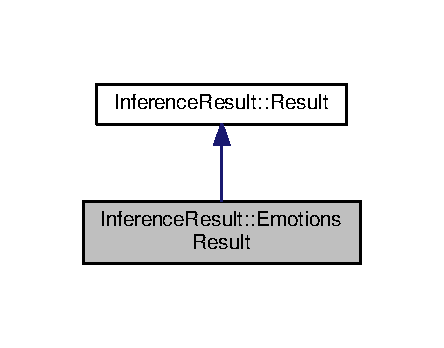
\includegraphics[width=213pt]{structInferenceResult_1_1EmotionsResult__inherit__graph}
\end{center}
\end{figure}


Collaboration diagram for Inference\+Result\+:\+:Emotions\+Result\+:
\nopagebreak
\begin{figure}[H]
\begin{center}
\leavevmode
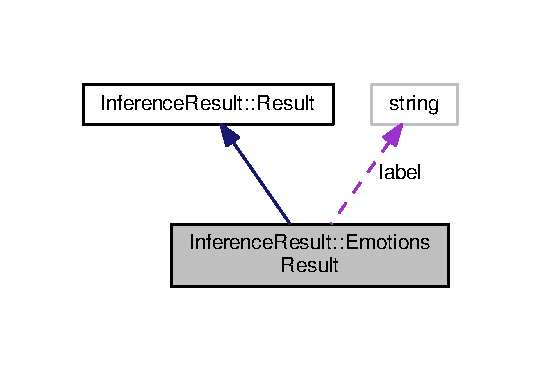
\includegraphics[width=260pt]{structInferenceResult_1_1EmotionsResult__coll__graph}
\end{center}
\end{figure}
\subsection*{Public Attributes}
\begin{DoxyCompactItemize}
\item 
std\+::string \hyperlink{structInferenceResult_1_1EmotionsResult_a273570a13673f51115a9de954cb0d333}{label} = \char`\"{}\char`\"{}
\item 
float \hyperlink{structInferenceResult_1_1EmotionsResult_aec1805367ebc6acda383d180a3cc896e}{confidence} = -\/1
\end{DoxyCompactItemize}


\subsection{Detailed Description}


Definition at line 21 of file data\+\_\+struct.\+h.



\subsection{Member Data Documentation}
\index{Inference\+Result\+::\+Emotions\+Result@{Inference\+Result\+::\+Emotions\+Result}!confidence@{confidence}}
\index{confidence@{confidence}!Inference\+Result\+::\+Emotions\+Result@{Inference\+Result\+::\+Emotions\+Result}}
\subsubsection[{\texorpdfstring{confidence}{confidence}}]{\setlength{\rightskip}{0pt plus 5cm}float Inference\+Result\+::\+Emotions\+Result\+::confidence = -\/1}\hypertarget{structInferenceResult_1_1EmotionsResult_aec1805367ebc6acda383d180a3cc896e}{}\label{structInferenceResult_1_1EmotionsResult_aec1805367ebc6acda383d180a3cc896e}


Definition at line 23 of file data\+\_\+struct.\+h.

\index{Inference\+Result\+::\+Emotions\+Result@{Inference\+Result\+::\+Emotions\+Result}!label@{label}}
\index{label@{label}!Inference\+Result\+::\+Emotions\+Result@{Inference\+Result\+::\+Emotions\+Result}}
\subsubsection[{\texorpdfstring{label}{label}}]{\setlength{\rightskip}{0pt plus 5cm}std\+::string Inference\+Result\+::\+Emotions\+Result\+::label = \char`\"{}\char`\"{}}\hypertarget{structInferenceResult_1_1EmotionsResult_a273570a13673f51115a9de954cb0d333}{}\label{structInferenceResult_1_1EmotionsResult_a273570a13673f51115a9de954cb0d333}


Definition at line 22 of file data\+\_\+struct.\+h.



The documentation for this struct was generated from the following file\+:\begin{DoxyCompactItemize}
\item 
include/openvino\+\_\+service/\hyperlink{data__struct_8h}{data\+\_\+struct.\+h}\end{DoxyCompactItemize}

\hypertarget{structInferenceEngine_1_1Extensions_1_1Cpu_1_1ExtensionsHolder}{}\section{Inference\+Engine\+:\+:Extensions\+:\+:Cpu\+:\+:Extensions\+Holder Struct Reference}
\label{structInferenceEngine_1_1Extensions_1_1Cpu_1_1ExtensionsHolder}\index{Inference\+Engine\+::\+Extensions\+::\+Cpu\+::\+Extensions\+Holder@{Inference\+Engine\+::\+Extensions\+::\+Cpu\+::\+Extensions\+Holder}}


{\ttfamily \#include $<$ext\+\_\+list.\+hpp$>$}

\subsection*{Public Attributes}
\begin{DoxyCompactItemize}
\item 
std\+::map$<$ std\+::string, \hyperlink{namespaceInferenceEngine_1_1Extensions_1_1Cpu_af4abba10662fceb8a076b617209801ed}{ext\+\_\+factory} $>$ \hyperlink{structInferenceEngine_1_1Extensions_1_1Cpu_1_1ExtensionsHolder_a169af915f746c7a77f5b02d5ef4b81be}{list}
\end{DoxyCompactItemize}


\subsection{Detailed Description}


Definition at line 33 of file ext\+\_\+list.\+hpp.



\subsection{Member Data Documentation}
\index{Inference\+Engine\+::\+Extensions\+::\+Cpu\+::\+Extensions\+Holder@{Inference\+Engine\+::\+Extensions\+::\+Cpu\+::\+Extensions\+Holder}!list@{list}}
\index{list@{list}!Inference\+Engine\+::\+Extensions\+::\+Cpu\+::\+Extensions\+Holder@{Inference\+Engine\+::\+Extensions\+::\+Cpu\+::\+Extensions\+Holder}}
\subsubsection[{\texorpdfstring{list}{list}}]{\setlength{\rightskip}{0pt plus 5cm}std\+::map$<$std\+::string, {\bf ext\+\_\+factory}$>$ Inference\+Engine\+::\+Extensions\+::\+Cpu\+::\+Extensions\+Holder\+::list}\hypertarget{structInferenceEngine_1_1Extensions_1_1Cpu_1_1ExtensionsHolder_a169af915f746c7a77f5b02d5ef4b81be}{}\label{structInferenceEngine_1_1Extensions_1_1Cpu_1_1ExtensionsHolder_a169af915f746c7a77f5b02d5ef4b81be}


Definition at line 34 of file ext\+\_\+list.\+hpp.



The documentation for this struct was generated from the following file\+:\begin{DoxyCompactItemize}
\item 
thirdparty/extension/\hyperlink{ext__list_8hpp}{ext\+\_\+list.\+hpp}\end{DoxyCompactItemize}

\hypertarget{classInferenceEngine_1_1Extensions_1_1Cpu_1_1ExtLayerBase}{}\section{Inference\+Engine\+:\+:Extensions\+:\+:Cpu\+:\+:Ext\+Layer\+Base Class Reference}
\label{classInferenceEngine_1_1Extensions_1_1Cpu_1_1ExtLayerBase}\index{Inference\+Engine\+::\+Extensions\+::\+Cpu\+::\+Ext\+Layer\+Base@{Inference\+Engine\+::\+Extensions\+::\+Cpu\+::\+Ext\+Layer\+Base}}


{\ttfamily \#include $<$ext\+\_\+base.\+hpp$>$}



Inheritance diagram for Inference\+Engine\+:\+:Extensions\+:\+:Cpu\+:\+:Ext\+Layer\+Base\+:
\nopagebreak
\begin{figure}[H]
\begin{center}
\leavevmode
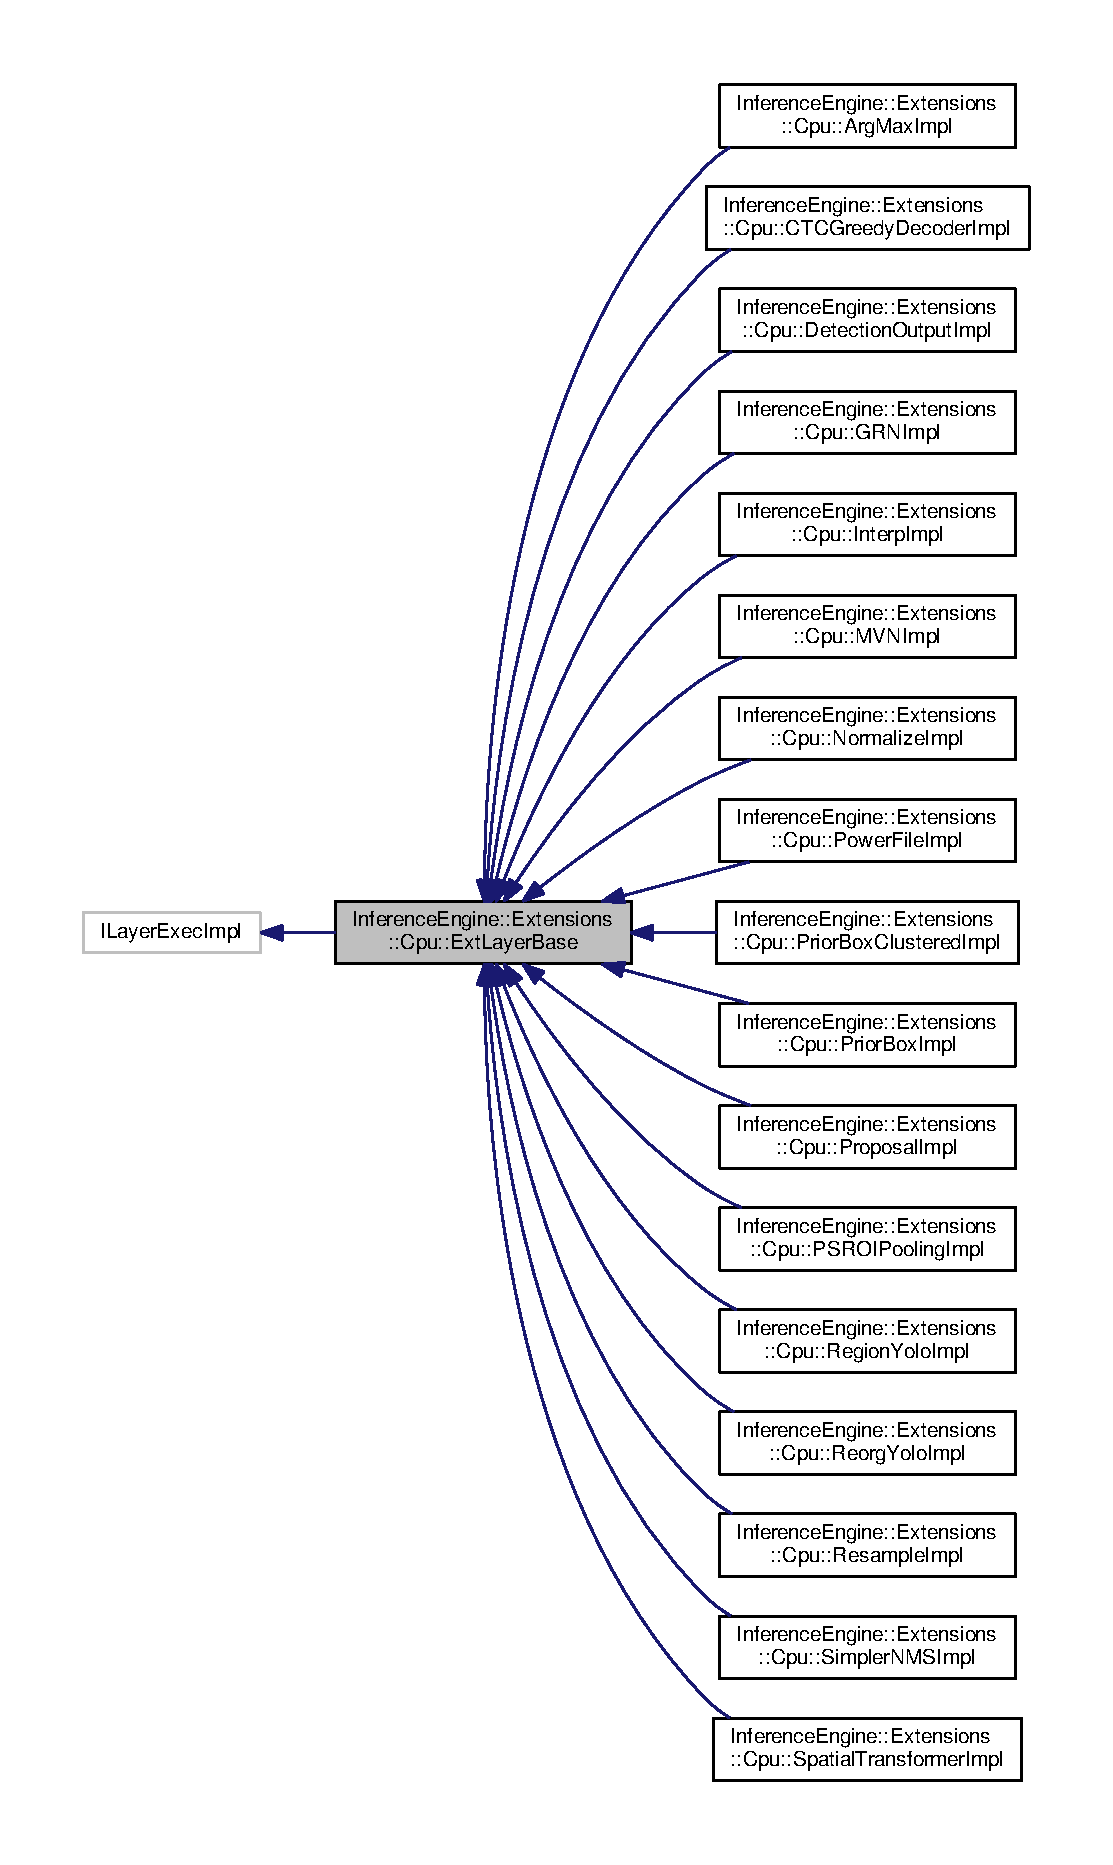
\includegraphics[height=550pt]{classInferenceEngine_1_1Extensions_1_1Cpu_1_1ExtLayerBase__inherit__graph}
\end{center}
\end{figure}


Collaboration diagram for Inference\+Engine\+:\+:Extensions\+:\+:Cpu\+:\+:Ext\+Layer\+Base\+:
\nopagebreak
\begin{figure}[H]
\begin{center}
\leavevmode
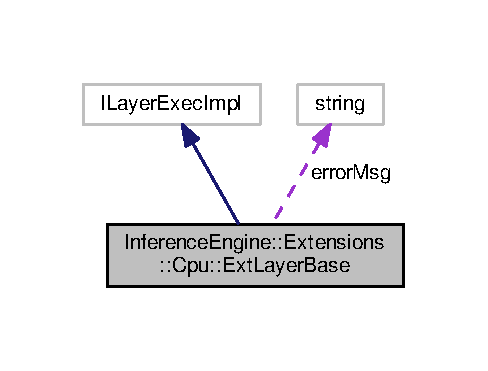
\includegraphics[width=234pt]{classInferenceEngine_1_1Extensions_1_1Cpu_1_1ExtLayerBase__coll__graph}
\end{center}
\end{figure}
\subsection*{Classes}
\begin{DoxyCompactItemize}
\item 
class \hyperlink{classInferenceEngine_1_1Extensions_1_1Cpu_1_1ExtLayerBase_1_1DataConfigurator}{Data\+Configurator}
\end{DoxyCompactItemize}
\subsection*{Public Member Functions}
\begin{DoxyCompactItemize}
\item 
\hyperlink{classInferenceEngine_1_1Extensions_1_1Cpu_1_1ExtLayerBase_affff0e8263ca26852ccf71d299d7b06a}{Ext\+Layer\+Base} (const C\+N\+N\+Layer $\ast$layer)
\item 
Status\+Code \hyperlink{classInferenceEngine_1_1Extensions_1_1Cpu_1_1ExtLayerBase_a1dae3d7d80ed72136ff298b90a5af266}{get\+Supported\+Configurations} (std\+::vector$<$ Layer\+Config $>$ \&conf, Response\+Desc $\ast$resp) noexceptoverride
\item 
Status\+Code \hyperlink{classInferenceEngine_1_1Extensions_1_1Cpu_1_1ExtLayerBase_a6323eec85cc894aa9ee19ae2b7443efb}{init} (Layer\+Config \&config, Response\+Desc $\ast$resp) noexceptoverride
\end{DoxyCompactItemize}
\subsection*{Protected Types}
\begin{DoxyCompactItemize}
\item 
enum \hyperlink{classInferenceEngine_1_1Extensions_1_1Cpu_1_1ExtLayerBase_a1258a8d209e0249e0b1717618352ddfb}{Conf\+Layout} \{ \hyperlink{classInferenceEngine_1_1Extensions_1_1Cpu_1_1ExtLayerBase_a1258a8d209e0249e0b1717618352ddfba8e1bde3c3d303163521522cf1d62f21f}{Conf\+Layout\+::\+A\+NY}, 
\hyperlink{classInferenceEngine_1_1Extensions_1_1Cpu_1_1ExtLayerBase_a1258a8d209e0249e0b1717618352ddfba446687ea2db1ada75be5ed053be77f59}{Conf\+Layout\+::\+P\+LN}, 
\hyperlink{classInferenceEngine_1_1Extensions_1_1Cpu_1_1ExtLayerBase_a1258a8d209e0249e0b1717618352ddfba6023b7e0a175b8cf9cbcec3ac3cbf93d}{Conf\+Layout\+::\+B\+L\+K8}, 
\hyperlink{classInferenceEngine_1_1Extensions_1_1Cpu_1_1ExtLayerBase_a1258a8d209e0249e0b1717618352ddfba733623e98c6602d47f51e9f7be2f7d6c}{Conf\+Layout\+::\+B\+L\+K16}
 \}
\end{DoxyCompactItemize}
\subsection*{Protected Member Functions}
\begin{DoxyCompactItemize}
\item 
void \hyperlink{classInferenceEngine_1_1Extensions_1_1Cpu_1_1ExtLayerBase_a0ac7a6632e95b9500d5246b05b4b0bfa}{add\+Config} (std\+::vector$<$ \hyperlink{classInferenceEngine_1_1Extensions_1_1Cpu_1_1ExtLayerBase_1_1DataConfigurator}{Data\+Configurator} $>$ in\+\_\+l, std\+::vector$<$ \hyperlink{classInferenceEngine_1_1Extensions_1_1Cpu_1_1ExtLayerBase_1_1DataConfigurator}{Data\+Configurator} $>$ out\+\_\+l, bool dyn\+Batch\+Support=false)
\end{DoxyCompactItemize}
\subsection*{Protected Attributes}
\begin{DoxyCompactItemize}
\item 
std\+::string \hyperlink{classInferenceEngine_1_1Extensions_1_1Cpu_1_1ExtLayerBase_abc78e9b5a79fa339ffd831a5318f71f7}{error\+Msg}
\item 
C\+N\+N\+Layer \hyperlink{classInferenceEngine_1_1Extensions_1_1Cpu_1_1ExtLayerBase_a1074cdccacb9e9ca6eec01bbc2f7ca4a}{cnn\+Layer}
\item 
std\+::vector$<$ Layer\+Config $>$ \hyperlink{classInferenceEngine_1_1Extensions_1_1Cpu_1_1ExtLayerBase_a2a9f897007f2eb00e295cd25fd23fd5d}{confs}
\end{DoxyCompactItemize}


\subsection{Detailed Description}


Definition at line 28 of file ext\+\_\+base.\+hpp.



\subsection{Member Enumeration Documentation}
\index{Inference\+Engine\+::\+Extensions\+::\+Cpu\+::\+Ext\+Layer\+Base@{Inference\+Engine\+::\+Extensions\+::\+Cpu\+::\+Ext\+Layer\+Base}!Conf\+Layout@{Conf\+Layout}}
\index{Conf\+Layout@{Conf\+Layout}!Inference\+Engine\+::\+Extensions\+::\+Cpu\+::\+Ext\+Layer\+Base@{Inference\+Engine\+::\+Extensions\+::\+Cpu\+::\+Ext\+Layer\+Base}}
\subsubsection[{\texorpdfstring{Conf\+Layout}{ConfLayout}}]{\setlength{\rightskip}{0pt plus 5cm}enum {\bf Inference\+Engine\+::\+Extensions\+::\+Cpu\+::\+Ext\+Layer\+Base\+::\+Conf\+Layout}\hspace{0.3cm}{\ttfamily [strong]}, {\ttfamily [protected]}}\hypertarget{classInferenceEngine_1_1Extensions_1_1Cpu_1_1ExtLayerBase_a1258a8d209e0249e0b1717618352ddfb}{}\label{classInferenceEngine_1_1Extensions_1_1Cpu_1_1ExtLayerBase_a1258a8d209e0249e0b1717618352ddfb}
\begin{Desc}
\item[Enumerator]\par
\begin{description}
\index{A\+NY@{A\+NY}!Inference\+Engine\+::\+Extensions\+::\+Cpu\+::\+Ext\+Layer\+Base@{Inference\+Engine\+::\+Extensions\+::\+Cpu\+::\+Ext\+Layer\+Base}}\index{Inference\+Engine\+::\+Extensions\+::\+Cpu\+::\+Ext\+Layer\+Base@{Inference\+Engine\+::\+Extensions\+::\+Cpu\+::\+Ext\+Layer\+Base}!A\+NY@{A\+NY}}\item[{\em 
A\+NY\hypertarget{classInferenceEngine_1_1Extensions_1_1Cpu_1_1ExtLayerBase_a1258a8d209e0249e0b1717618352ddfba8e1bde3c3d303163521522cf1d62f21f}{}\label{classInferenceEngine_1_1Extensions_1_1Cpu_1_1ExtLayerBase_a1258a8d209e0249e0b1717618352ddfba8e1bde3c3d303163521522cf1d62f21f}
}]\index{P\+LN@{P\+LN}!Inference\+Engine\+::\+Extensions\+::\+Cpu\+::\+Ext\+Layer\+Base@{Inference\+Engine\+::\+Extensions\+::\+Cpu\+::\+Ext\+Layer\+Base}}\index{Inference\+Engine\+::\+Extensions\+::\+Cpu\+::\+Ext\+Layer\+Base@{Inference\+Engine\+::\+Extensions\+::\+Cpu\+::\+Ext\+Layer\+Base}!P\+LN@{P\+LN}}\item[{\em 
P\+LN\hypertarget{classInferenceEngine_1_1Extensions_1_1Cpu_1_1ExtLayerBase_a1258a8d209e0249e0b1717618352ddfba446687ea2db1ada75be5ed053be77f59}{}\label{classInferenceEngine_1_1Extensions_1_1Cpu_1_1ExtLayerBase_a1258a8d209e0249e0b1717618352ddfba446687ea2db1ada75be5ed053be77f59}
}]\index{B\+L\+K8@{B\+L\+K8}!Inference\+Engine\+::\+Extensions\+::\+Cpu\+::\+Ext\+Layer\+Base@{Inference\+Engine\+::\+Extensions\+::\+Cpu\+::\+Ext\+Layer\+Base}}\index{Inference\+Engine\+::\+Extensions\+::\+Cpu\+::\+Ext\+Layer\+Base@{Inference\+Engine\+::\+Extensions\+::\+Cpu\+::\+Ext\+Layer\+Base}!B\+L\+K8@{B\+L\+K8}}\item[{\em 
B\+L\+K8\hypertarget{classInferenceEngine_1_1Extensions_1_1Cpu_1_1ExtLayerBase_a1258a8d209e0249e0b1717618352ddfba6023b7e0a175b8cf9cbcec3ac3cbf93d}{}\label{classInferenceEngine_1_1Extensions_1_1Cpu_1_1ExtLayerBase_a1258a8d209e0249e0b1717618352ddfba6023b7e0a175b8cf9cbcec3ac3cbf93d}
}]\index{B\+L\+K16@{B\+L\+K16}!Inference\+Engine\+::\+Extensions\+::\+Cpu\+::\+Ext\+Layer\+Base@{Inference\+Engine\+::\+Extensions\+::\+Cpu\+::\+Ext\+Layer\+Base}}\index{Inference\+Engine\+::\+Extensions\+::\+Cpu\+::\+Ext\+Layer\+Base@{Inference\+Engine\+::\+Extensions\+::\+Cpu\+::\+Ext\+Layer\+Base}!B\+L\+K16@{B\+L\+K16}}\item[{\em 
B\+L\+K16\hypertarget{classInferenceEngine_1_1Extensions_1_1Cpu_1_1ExtLayerBase_a1258a8d209e0249e0b1717618352ddfba733623e98c6602d47f51e9f7be2f7d6c}{}\label{classInferenceEngine_1_1Extensions_1_1Cpu_1_1ExtLayerBase_a1258a8d209e0249e0b1717618352ddfba733623e98c6602d47f51e9f7be2f7d6c}
}]\end{description}
\end{Desc}


Definition at line 36 of file ext\+\_\+base.\+hpp.


\begin{DoxyCode}
36 \{ ANY, PLN, BLK8, BLK16 \};
\end{DoxyCode}


\subsection{Constructor \& Destructor Documentation}
\index{Inference\+Engine\+::\+Extensions\+::\+Cpu\+::\+Ext\+Layer\+Base@{Inference\+Engine\+::\+Extensions\+::\+Cpu\+::\+Ext\+Layer\+Base}!Ext\+Layer\+Base@{Ext\+Layer\+Base}}
\index{Ext\+Layer\+Base@{Ext\+Layer\+Base}!Inference\+Engine\+::\+Extensions\+::\+Cpu\+::\+Ext\+Layer\+Base@{Inference\+Engine\+::\+Extensions\+::\+Cpu\+::\+Ext\+Layer\+Base}}
\subsubsection[{\texorpdfstring{Ext\+Layer\+Base(const C\+N\+N\+Layer $\ast$layer)}{ExtLayerBase(const CNNLayer *layer)}}]{\setlength{\rightskip}{0pt plus 5cm}Inference\+Engine\+::\+Extensions\+::\+Cpu\+::\+Ext\+Layer\+Base\+::\+Ext\+Layer\+Base (
\begin{DoxyParamCaption}
\item[{const C\+N\+N\+Layer $\ast$}]{layer}
\end{DoxyParamCaption}
)\hspace{0.3cm}{\ttfamily [inline]}, {\ttfamily [explicit]}}\hypertarget{classInferenceEngine_1_1Extensions_1_1Cpu_1_1ExtLayerBase_affff0e8263ca26852ccf71d299d7b06a}{}\label{classInferenceEngine_1_1Extensions_1_1Cpu_1_1ExtLayerBase_affff0e8263ca26852ccf71d299d7b06a}


Definition at line 30 of file ext\+\_\+base.\+hpp.


\begin{DoxyCode}
30 : \hyperlink{classInferenceEngine_1_1Extensions_1_1Cpu_1_1ExtLayerBase_a1074cdccacb9e9ca6eec01bbc2f7ca4a}{cnnLayer}(*layer) \{\}
\end{DoxyCode}


\subsection{Member Function Documentation}
\index{Inference\+Engine\+::\+Extensions\+::\+Cpu\+::\+Ext\+Layer\+Base@{Inference\+Engine\+::\+Extensions\+::\+Cpu\+::\+Ext\+Layer\+Base}!add\+Config@{add\+Config}}
\index{add\+Config@{add\+Config}!Inference\+Engine\+::\+Extensions\+::\+Cpu\+::\+Ext\+Layer\+Base@{Inference\+Engine\+::\+Extensions\+::\+Cpu\+::\+Ext\+Layer\+Base}}
\subsubsection[{\texorpdfstring{add\+Config(std\+::vector$<$ Data\+Configurator $>$ in\+\_\+l, std\+::vector$<$ Data\+Configurator $>$ out\+\_\+l, bool dyn\+Batch\+Support=false)}{addConfig(std::vector< DataConfigurator > in_l, std::vector< DataConfigurator > out_l, bool dynBatchSupport=false)}}]{\setlength{\rightskip}{0pt plus 5cm}void Inference\+Engine\+::\+Extensions\+::\+Cpu\+::\+Ext\+Layer\+Base\+::add\+Config (
\begin{DoxyParamCaption}
\item[{std\+::vector$<$ {\bf Data\+Configurator} $>$}]{in\+\_\+l, }
\item[{std\+::vector$<$ {\bf Data\+Configurator} $>$}]{out\+\_\+l, }
\item[{bool}]{dyn\+Batch\+Support = {\ttfamily false}}
\end{DoxyParamCaption}
)\hspace{0.3cm}{\ttfamily [protected]}}\hypertarget{classInferenceEngine_1_1Extensions_1_1Cpu_1_1ExtLayerBase_a0ac7a6632e95b9500d5246b05b4b0bfa}{}\label{classInferenceEngine_1_1Extensions_1_1Cpu_1_1ExtLayerBase_a0ac7a6632e95b9500d5246b05b4b0bfa}


Definition at line 70 of file ext\+\_\+base.\+cpp.


\begin{DoxyCode}
70                                                                                                            
                 \{
71     LayerConfig config;
72 
73     \textcolor{keywordflow}{if} (in\_l.size() != \hyperlink{classInferenceEngine_1_1Extensions_1_1Cpu_1_1ExtLayerBase_a1074cdccacb9e9ca6eec01bbc2f7ca4a}{cnnLayer}.insData.size())
74         THROW\_IE\_EXCEPTION << \textcolor{stringliteral}{"Incorrect number of input edges. Expected "} << 
      \hyperlink{classInferenceEngine_1_1Extensions_1_1Cpu_1_1ExtLayerBase_a1074cdccacb9e9ca6eec01bbc2f7ca4a}{cnnLayer}.insData.size()
75                            << \textcolor{stringliteral}{" but layout specification provided for "} << in\_l.size();
76     \textcolor{keywordflow}{if} (out\_l.size() != \hyperlink{classInferenceEngine_1_1Extensions_1_1Cpu_1_1ExtLayerBase_a1074cdccacb9e9ca6eec01bbc2f7ca4a}{cnnLayer}.outData.size())
77         THROW\_IE\_EXCEPTION << \textcolor{stringliteral}{"Incorrect number of input edges. Expected "} << 
      \hyperlink{classInferenceEngine_1_1Extensions_1_1Cpu_1_1ExtLayerBase_a1074cdccacb9e9ca6eec01bbc2f7ca4a}{cnnLayer}.outData.size()
78                            << \textcolor{stringliteral}{" but layout specification provided for "} << out\_l.size();
79 
80     \textcolor{comment}{// Fill tensor parameters into config}
81     \textcolor{keyword}{auto} fill\_port = [] (std::vector<DataConfig>& port, DataConfigurator conf, \textcolor{keyword}{const} DataPtr& data) \{
82         \textcolor{keywordflow}{if} (!data) THROW\_IE\_EXCEPTION << \textcolor{stringliteral}{"Cannot get input data!"};
83 
84         DataConfig dataConfig;
85         dataConfig.inPlace = conf.inplace;
86         dataConfig.constant = conf.constant;
87 
88         \textcolor{keyword}{const} TensorDesc& data\_desc = data->getTensorDesc();
89         \textcolor{keyword}{const} SizeVector& data\_dims = data\_desc.getDims();
90 
91         std::vector<size\_t> blocks = data\_dims;
92         std::vector<size\_t> order(blocks.size());
93         \textcolor{keywordflow}{for} (\textcolor{keywordtype}{size\_t} i = 0; i < order.size(); i++) order[i] = i;
94 
95         \textcolor{keywordflow}{if} (conf.layout == \hyperlink{classInferenceEngine_1_1Extensions_1_1Cpu_1_1ExtLayerBase_a1258a8d209e0249e0b1717618352ddfba6023b7e0a175b8cf9cbcec3ac3cbf93d}{ConfLayout::BLK8} || conf.layout == 
      \hyperlink{classInferenceEngine_1_1Extensions_1_1Cpu_1_1ExtLayerBase_a1258a8d209e0249e0b1717618352ddfba733623e98c6602d47f51e9f7be2f7d6c}{ConfLayout::BLK16}) \{
96             \textcolor{keywordflow}{if} (data\_dims.size() != 4)
97                 THROW\_IE\_EXCEPTION << \textcolor{stringliteral}{"Inapplicable blocking layout."}
98                                    << \textcolor{stringliteral}{"Tensor should be 4D."};
99 
100             \textcolor{keywordtype}{int} blk\_size = conf.layout == \hyperlink{classInferenceEngine_1_1Extensions_1_1Cpu_1_1ExtLayerBase_a1258a8d209e0249e0b1717618352ddfba6023b7e0a175b8cf9cbcec3ac3cbf93d}{ConfLayout::BLK8} ? 8 : 16;
101 
102             \textcolor{comment}{// Blocking through Channel dimension. Like [nChwXc]}
103             order.push\_back(1);
104             blocks[1] = \hyperlink{namespaceInferenceEngine_1_1Extensions_1_1Cpu_a979bf0275746a13e636116a432953b15}{div\_up}(blocks[1], blk\_size);
105             blocks.push\_back(blk\_size);
106         \}
107 
108         \textcolor{comment}{// All extension layers support only FP32 precision!}
109         InferenceEngine::Precision precision = conf.constant ? data\_desc.getPrecision() : 
      InferenceEngine::Precision(InferenceEngine::Precision::FP32);
110         \textcolor{keywordflow}{if} (conf.layout == \hyperlink{classInferenceEngine_1_1Extensions_1_1Cpu_1_1ExtLayerBase_a1258a8d209e0249e0b1717618352ddfba8e1bde3c3d303163521522cf1d62f21f}{ConfLayout::ANY}) \{
111             dataConfig.desc = TensorDesc(precision, data\_dims, InferenceEngine::Layout::ANY);
112         \} \textcolor{keywordflow}{else} \{
113             dataConfig.desc = TensorDesc(precision, data\_dims, \{blocks, order\});
114         \}
115         port.push\_back(dataConfig);
116     \};
117 
118     \textcolor{keywordflow}{for} (\textcolor{keywordtype}{int} i = 0; i < in\_l.size(); i++)
119         fill\_port(config.inConfs, in\_l[i], \hyperlink{classInferenceEngine_1_1Extensions_1_1Cpu_1_1ExtLayerBase_a1074cdccacb9e9ca6eec01bbc2f7ca4a}{cnnLayer}.insData[i].lock());
120 
121     \textcolor{keywordflow}{for} (\textcolor{keywordtype}{int} i = 0; i < out\_l.size(); i++)
122         fill\_port(config.outConfs, out\_l[i], \hyperlink{classInferenceEngine_1_1Extensions_1_1Cpu_1_1ExtLayerBase_a1074cdccacb9e9ca6eec01bbc2f7ca4a}{cnnLayer}.outData[i]);
123 
124     config.dynBatchSupport = dynBatchSupport;
125     \hyperlink{classInferenceEngine_1_1Extensions_1_1Cpu_1_1ExtLayerBase_a2a9f897007f2eb00e295cd25fd23fd5d}{confs}.push\_back(config);
126 \}
\end{DoxyCode}
\index{Inference\+Engine\+::\+Extensions\+::\+Cpu\+::\+Ext\+Layer\+Base@{Inference\+Engine\+::\+Extensions\+::\+Cpu\+::\+Ext\+Layer\+Base}!get\+Supported\+Configurations@{get\+Supported\+Configurations}}
\index{get\+Supported\+Configurations@{get\+Supported\+Configurations}!Inference\+Engine\+::\+Extensions\+::\+Cpu\+::\+Ext\+Layer\+Base@{Inference\+Engine\+::\+Extensions\+::\+Cpu\+::\+Ext\+Layer\+Base}}
\subsubsection[{\texorpdfstring{get\+Supported\+Configurations(std\+::vector$<$ Layer\+Config $>$ \&conf, Response\+Desc $\ast$resp) noexceptoverride}{getSupportedConfigurations(std::vector< LayerConfig > &conf, ResponseDesc *resp) noexceptoverride}}]{\setlength{\rightskip}{0pt plus 5cm}Status\+Code Inference\+Engine\+::\+Extensions\+::\+Cpu\+::\+Ext\+Layer\+Base\+::get\+Supported\+Configurations (
\begin{DoxyParamCaption}
\item[{std\+::vector$<$ Layer\+Config $>$ \&}]{conf, }
\item[{Response\+Desc $\ast$}]{resp}
\end{DoxyParamCaption}
)\hspace{0.3cm}{\ttfamily [override]}, {\ttfamily [noexcept]}}\hypertarget{classInferenceEngine_1_1Extensions_1_1Cpu_1_1ExtLayerBase_a1dae3d7d80ed72136ff298b90a5af266}{}\label{classInferenceEngine_1_1Extensions_1_1Cpu_1_1ExtLayerBase_a1dae3d7d80ed72136ff298b90a5af266}


Definition at line 34 of file ext\+\_\+base.\+cpp.


\begin{DoxyCode}
34                                                                                                   \{
35     \textcolor{keywordflow}{if} (!\hyperlink{classInferenceEngine_1_1Extensions_1_1Cpu_1_1ExtLayerBase_abc78e9b5a79fa339ffd831a5318f71f7}{errorMsg}.empty()) \{
36         \textcolor{keywordflow}{if} (resp) \{
37             \hyperlink{classInferenceEngine_1_1Extensions_1_1Cpu_1_1ExtLayerBase_abc78e9b5a79fa339ffd831a5318f71f7}{errorMsg}.copy(resp->msg, \textcolor{keyword}{sizeof}(resp->msg) - 1);
38         \}
39         \textcolor{keywordflow}{return} GENERAL\_ERROR;
40     \}
41     conf = \hyperlink{classInferenceEngine_1_1Extensions_1_1Cpu_1_1ExtLayerBase_a2a9f897007f2eb00e295cd25fd23fd5d}{confs};
42     \textcolor{keywordflow}{return} OK;
43 \}
\end{DoxyCode}
\index{Inference\+Engine\+::\+Extensions\+::\+Cpu\+::\+Ext\+Layer\+Base@{Inference\+Engine\+::\+Extensions\+::\+Cpu\+::\+Ext\+Layer\+Base}!init@{init}}
\index{init@{init}!Inference\+Engine\+::\+Extensions\+::\+Cpu\+::\+Ext\+Layer\+Base@{Inference\+Engine\+::\+Extensions\+::\+Cpu\+::\+Ext\+Layer\+Base}}
\subsubsection[{\texorpdfstring{init(\+Layer\+Config \&config, Response\+Desc $\ast$resp) noexceptoverride}{init(LayerConfig &config, ResponseDesc *resp) noexceptoverride}}]{\setlength{\rightskip}{0pt plus 5cm}Status\+Code Inference\+Engine\+::\+Extensions\+::\+Cpu\+::\+Ext\+Layer\+Base\+::init (
\begin{DoxyParamCaption}
\item[{Layer\+Config \&}]{config, }
\item[{Response\+Desc $\ast$}]{resp}
\end{DoxyParamCaption}
)\hspace{0.3cm}{\ttfamily [override]}, {\ttfamily [noexcept]}}\hypertarget{classInferenceEngine_1_1Extensions_1_1Cpu_1_1ExtLayerBase_a6323eec85cc894aa9ee19ae2b7443efb}{}\label{classInferenceEngine_1_1Extensions_1_1Cpu_1_1ExtLayerBase_a6323eec85cc894aa9ee19ae2b7443efb}


Definition at line 46 of file ext\+\_\+base.\+cpp.


\begin{DoxyCode}
46                                                                    \{
47     \textcolor{keywordflow}{for} (\textcolor{keyword}{auto}& input : config.inConfs) \{
48         \textcolor{keywordflow}{for} (\textcolor{keyword}{auto}& offset : input.desc.getBlockingDesc().getOffsetPaddingToData()) \{
49             \textcolor{keywordflow}{if} (offset) \{
50                 \textcolor{keywordflow}{return} GENERAL\_ERROR;
51             \}
52         \}
53         \textcolor{keywordflow}{if} (input.desc.getBlockingDesc().getOffsetPadding()) \{
54             \textcolor{keywordflow}{return} GENERAL\_ERROR;
55         \}
56     \}
57     \textcolor{keywordflow}{for} (\textcolor{keyword}{auto}& output : config.outConfs) \{
58         \textcolor{keywordflow}{for} (\textcolor{keyword}{auto}& offset : output.desc.getBlockingDesc().getOffsetPaddingToData()) \{
59             \textcolor{keywordflow}{if} (offset) \{
60                 \textcolor{keywordflow}{return} GENERAL\_ERROR;
61             \}
62         \}
63         \textcolor{keywordflow}{if} (output.desc.getBlockingDesc().getOffsetPadding()) \{
64             \textcolor{keywordflow}{return} GENERAL\_ERROR;
65         \}
66     \}
67     \textcolor{keywordflow}{return} OK;
68 \}
\end{DoxyCode}


\subsection{Member Data Documentation}
\index{Inference\+Engine\+::\+Extensions\+::\+Cpu\+::\+Ext\+Layer\+Base@{Inference\+Engine\+::\+Extensions\+::\+Cpu\+::\+Ext\+Layer\+Base}!cnn\+Layer@{cnn\+Layer}}
\index{cnn\+Layer@{cnn\+Layer}!Inference\+Engine\+::\+Extensions\+::\+Cpu\+::\+Ext\+Layer\+Base@{Inference\+Engine\+::\+Extensions\+::\+Cpu\+::\+Ext\+Layer\+Base}}
\subsubsection[{\texorpdfstring{cnn\+Layer}{cnnLayer}}]{\setlength{\rightskip}{0pt plus 5cm}C\+N\+N\+Layer Inference\+Engine\+::\+Extensions\+::\+Cpu\+::\+Ext\+Layer\+Base\+::cnn\+Layer\hspace{0.3cm}{\ttfamily [protected]}}\hypertarget{classInferenceEngine_1_1Extensions_1_1Cpu_1_1ExtLayerBase_a1074cdccacb9e9ca6eec01bbc2f7ca4a}{}\label{classInferenceEngine_1_1Extensions_1_1Cpu_1_1ExtLayerBase_a1074cdccacb9e9ca6eec01bbc2f7ca4a}


Definition at line 53 of file ext\+\_\+base.\+hpp.

\index{Inference\+Engine\+::\+Extensions\+::\+Cpu\+::\+Ext\+Layer\+Base@{Inference\+Engine\+::\+Extensions\+::\+Cpu\+::\+Ext\+Layer\+Base}!confs@{confs}}
\index{confs@{confs}!Inference\+Engine\+::\+Extensions\+::\+Cpu\+::\+Ext\+Layer\+Base@{Inference\+Engine\+::\+Extensions\+::\+Cpu\+::\+Ext\+Layer\+Base}}
\subsubsection[{\texorpdfstring{confs}{confs}}]{\setlength{\rightskip}{0pt plus 5cm}std\+::vector$<$Layer\+Config$>$ Inference\+Engine\+::\+Extensions\+::\+Cpu\+::\+Ext\+Layer\+Base\+::confs\hspace{0.3cm}{\ttfamily [protected]}}\hypertarget{classInferenceEngine_1_1Extensions_1_1Cpu_1_1ExtLayerBase_a2a9f897007f2eb00e295cd25fd23fd5d}{}\label{classInferenceEngine_1_1Extensions_1_1Cpu_1_1ExtLayerBase_a2a9f897007f2eb00e295cd25fd23fd5d}


Definition at line 54 of file ext\+\_\+base.\+hpp.

\index{Inference\+Engine\+::\+Extensions\+::\+Cpu\+::\+Ext\+Layer\+Base@{Inference\+Engine\+::\+Extensions\+::\+Cpu\+::\+Ext\+Layer\+Base}!error\+Msg@{error\+Msg}}
\index{error\+Msg@{error\+Msg}!Inference\+Engine\+::\+Extensions\+::\+Cpu\+::\+Ext\+Layer\+Base@{Inference\+Engine\+::\+Extensions\+::\+Cpu\+::\+Ext\+Layer\+Base}}
\subsubsection[{\texorpdfstring{error\+Msg}{errorMsg}}]{\setlength{\rightskip}{0pt plus 5cm}std\+::string Inference\+Engine\+::\+Extensions\+::\+Cpu\+::\+Ext\+Layer\+Base\+::error\+Msg\hspace{0.3cm}{\ttfamily [protected]}}\hypertarget{classInferenceEngine_1_1Extensions_1_1Cpu_1_1ExtLayerBase_abc78e9b5a79fa339ffd831a5318f71f7}{}\label{classInferenceEngine_1_1Extensions_1_1Cpu_1_1ExtLayerBase_abc78e9b5a79fa339ffd831a5318f71f7}


Definition at line 52 of file ext\+\_\+base.\+hpp.



The documentation for this class was generated from the following files\+:\begin{DoxyCompactItemize}
\item 
thirdparty/extension/\hyperlink{ext__base_8hpp}{ext\+\_\+base.\+hpp}\item 
thirdparty/extension/\hyperlink{ext__base_8cpp}{ext\+\_\+base.\+cpp}\end{DoxyCompactItemize}

\hypertarget{classInferenceEngine_1_1Extensions_1_1Cpu_1_1ExtRegisterBase}{}\section{Inference\+Engine\+:\+:Extensions\+:\+:Cpu\+:\+:Ext\+Register\+Base$<$ Ext $>$ Class Template Reference}
\label{classInferenceEngine_1_1Extensions_1_1Cpu_1_1ExtRegisterBase}\index{Inference\+Engine\+::\+Extensions\+::\+Cpu\+::\+Ext\+Register\+Base$<$ Ext $>$@{Inference\+Engine\+::\+Extensions\+::\+Cpu\+::\+Ext\+Register\+Base$<$ Ext $>$}}


{\ttfamily \#include $<$ext\+\_\+list.\+hpp$>$}

\subsection*{Public Member Functions}
\begin{DoxyCompactItemize}
\item 
\hyperlink{classInferenceEngine_1_1Extensions_1_1Cpu_1_1ExtRegisterBase_a1d56b4f9730d0e019c31539654c666ee}{Ext\+Register\+Base} (const std\+::string \&type)
\end{DoxyCompactItemize}


\subsection{Detailed Description}
\subsubsection*{template$<$typename Ext$>$\\*
class Inference\+Engine\+::\+Extensions\+::\+Cpu\+::\+Ext\+Register\+Base$<$ Ext $>$}



Definition at line 69 of file ext\+\_\+list.\+hpp.



\subsection{Constructor \& Destructor Documentation}
\index{Inference\+Engine\+::\+Extensions\+::\+Cpu\+::\+Ext\+Register\+Base@{Inference\+Engine\+::\+Extensions\+::\+Cpu\+::\+Ext\+Register\+Base}!Ext\+Register\+Base@{Ext\+Register\+Base}}
\index{Ext\+Register\+Base@{Ext\+Register\+Base}!Inference\+Engine\+::\+Extensions\+::\+Cpu\+::\+Ext\+Register\+Base@{Inference\+Engine\+::\+Extensions\+::\+Cpu\+::\+Ext\+Register\+Base}}
\subsubsection[{\texorpdfstring{Ext\+Register\+Base(const std\+::string \&type)}{ExtRegisterBase(const std::string &type)}}]{\setlength{\rightskip}{0pt plus 5cm}template$<$typename Ext $>$ {\bf Inference\+Engine\+::\+Extensions\+::\+Cpu\+::\+Ext\+Register\+Base}$<$ Ext $>$\+::{\bf Ext\+Register\+Base} (
\begin{DoxyParamCaption}
\item[{const std\+::string \&}]{type}
\end{DoxyParamCaption}
)\hspace{0.3cm}{\ttfamily [inline]}, {\ttfamily [explicit]}}\hypertarget{classInferenceEngine_1_1Extensions_1_1Cpu_1_1ExtRegisterBase_a1d56b4f9730d0e019c31539654c666ee}{}\label{classInferenceEngine_1_1Extensions_1_1Cpu_1_1ExtRegisterBase_a1d56b4f9730d0e019c31539654c666ee}


Definition at line 71 of file ext\+\_\+list.\+hpp.


\begin{DoxyCode}
71                                                     \{
72         CpuExtensions::AddExt(type,
73             [](\textcolor{keyword}{const} CNNLayer *layer) -> InferenceEngine::ILayerImplFactory* \{
74                 \textcolor{keywordflow}{return} \textcolor{keyword}{new} Ext(layer);
75             \});
76     \}
\end{DoxyCode}


The documentation for this class was generated from the following file\+:\begin{DoxyCompactItemize}
\item 
thirdparty/extension/\hyperlink{ext__list_8hpp}{ext\+\_\+list.\+hpp}\end{DoxyCompactItemize}

\hypertarget{classopenvino__service_1_1FaceDetection}{}\section{openvino\+\_\+service\+:\+:Face\+Detection Class Reference}
\label{classopenvino__service_1_1FaceDetection}\index{openvino\+\_\+service\+::\+Face\+Detection@{openvino\+\_\+service\+::\+Face\+Detection}}


{\ttfamily \#include $<$face\+\_\+detection.\+h$>$}



Inheritance diagram for openvino\+\_\+service\+:\+:Face\+Detection\+:
\nopagebreak
\begin{figure}[H]
\begin{center}
\leavevmode
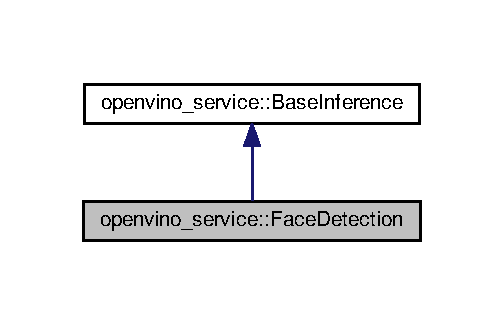
\includegraphics[width=242pt]{classopenvino__service_1_1FaceDetection__inherit__graph}
\end{center}
\end{figure}


Collaboration diagram for openvino\+\_\+service\+:\+:Face\+Detection\+:
\nopagebreak
\begin{figure}[H]
\begin{center}
\leavevmode
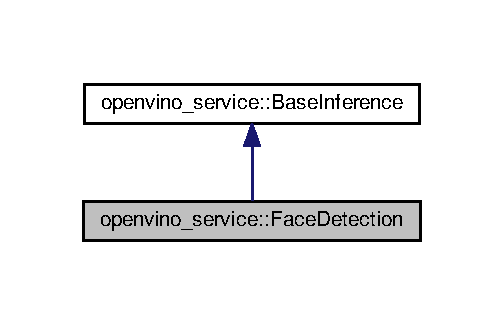
\includegraphics[width=242pt]{classopenvino__service_1_1FaceDetection__coll__graph}
\end{center}
\end{figure}
\subsection*{Public Types}
\begin{DoxyCompactItemize}
\item 
using \hyperlink{classopenvino__service_1_1FaceDetection_a35ec2b5ed353d7f08a5475df7cccb249}{Result} = \hyperlink{structInferenceResult_1_1FaceDetectionResult}{Inference\+Result\+::\+Face\+Detection\+Result}
\end{DoxyCompactItemize}
\subsection*{Public Member Functions}
\begin{DoxyCompactItemize}
\item 
\hyperlink{classopenvino__service_1_1FaceDetection_a7af587f1765e10fe57cb7e23fc11b972}{Face\+Detection} (\hyperlink{CMakeCache_8txt_a79a3d8790b2588b09777910863574e09}{int}, \hyperlink{CMakeCache_8txt_a79a3d8790b2588b09777910863574e09}{int}, double)
\item 
\hyperlink{classopenvino__service_1_1FaceDetection_ab7ca36b46bdc69a8f1ca582ed9494c06}{$\sim$\+Face\+Detection} () override
\item 
void \hyperlink{classopenvino__service_1_1FaceDetection_a6594d4aaefcbeee2d1f248891cc8fe86}{load\+Network} (std\+::shared\+\_\+ptr$<$ \hyperlink{classValidatedFaceDetectionNetwork}{Validated\+Face\+Detection\+Network} $>$)
\item 
bool \hyperlink{classopenvino__service_1_1FaceDetection_a7332817c496f2306b2a9ca3b45a7ec48}{enqueue} (const cv\+::\+Mat \&, const cv\+::\+Rect \&) override
\begin{DoxyCompactList}\small\item\em Enqueue a frame to this class. The frame will be buffered but not infered yet. \end{DoxyCompactList}\item 
bool \hyperlink{classopenvino__service_1_1FaceDetection_ad8c87c0d59af0f36030fed55a0bcec4b}{submit\+Request} () override
\begin{DoxyCompactList}\small\item\em Start inference for all buffered frames. \end{DoxyCompactList}\item 
bool \hyperlink{classopenvino__service_1_1FaceDetection_af3153d2032ed93c03aa0fa62b90f5526}{fetch\+Results} () override
\begin{DoxyCompactList}\small\item\em This function will fetch the results of the previous inference and stores the results in a result buffer array. All buffered frames will be cleared. \end{DoxyCompactList}\item 
void \hyperlink{classopenvino__service_1_1FaceDetection_a5c06d03813e7bf494f7908577d8392c5}{accepts} (std\+::shared\+\_\+ptr$<$ \hyperlink{classBaseOutput}{Base\+Output} $>$ output\+\_\+visitor) override
\begin{DoxyCompactList}\small\item\em Accepts an Output instance for result process. This function is used for visitor pattern. \end{DoxyCompactList}\item 
const \hyperlink{CMakeCache_8txt_a79a3d8790b2588b09777910863574e09}{int} \hyperlink{classopenvino__service_1_1FaceDetection_a778bb42884d67b286e4e9656fb0a69ef}{get\+Results\+Length} () const override
\begin{DoxyCompactList}\small\item\em Get the length of the buffer result array. \end{DoxyCompactList}\item 
const \hyperlink{structInferenceResult_1_1Result}{Inference\+Result\+::\+Result} \hyperlink{classopenvino__service_1_1FaceDetection_ab4dd44a79728c5d3961023a73d2ceb0c}{get\+Location\+Result} (\hyperlink{CMakeCache_8txt_a79a3d8790b2588b09777910863574e09}{int} idx) const override
\begin{DoxyCompactList}\small\item\em Get the location of result with respect to the frame generated by the input device. \end{DoxyCompactList}\item 
const std\+::string \hyperlink{classopenvino__service_1_1FaceDetection_ac815cdf8a4ca763f204d17beb5385f5f}{get\+Name} () const override
\begin{DoxyCompactList}\small\item\em Get the name of the Inference instance. \end{DoxyCompactList}\end{DoxyCompactItemize}
\subsection*{Additional Inherited Members}


\subsection{Detailed Description}


Definition at line 20 of file face\+\_\+detection.\+h.



\subsection{Member Typedef Documentation}
\index{openvino\+\_\+service\+::\+Face\+Detection@{openvino\+\_\+service\+::\+Face\+Detection}!Result@{Result}}
\index{Result@{Result}!openvino\+\_\+service\+::\+Face\+Detection@{openvino\+\_\+service\+::\+Face\+Detection}}
\subsubsection[{\texorpdfstring{Result}{Result}}]{\setlength{\rightskip}{0pt plus 5cm}using {\bf openvino\+\_\+service\+::\+Face\+Detection\+::\+Result} =  {\bf Inference\+Result\+::\+Face\+Detection\+Result}}\hypertarget{classopenvino__service_1_1FaceDetection_a35ec2b5ed353d7f08a5475df7cccb249}{}\label{classopenvino__service_1_1FaceDetection_a35ec2b5ed353d7f08a5475df7cccb249}


Definition at line 22 of file face\+\_\+detection.\+h.



\subsection{Constructor \& Destructor Documentation}
\index{openvino\+\_\+service\+::\+Face\+Detection@{openvino\+\_\+service\+::\+Face\+Detection}!Face\+Detection@{Face\+Detection}}
\index{Face\+Detection@{Face\+Detection}!openvino\+\_\+service\+::\+Face\+Detection@{openvino\+\_\+service\+::\+Face\+Detection}}
\subsubsection[{\texorpdfstring{Face\+Detection(int, int, double)}{FaceDetection(int, int, double)}}]{\setlength{\rightskip}{0pt plus 5cm}openvino\+\_\+service\+::\+Face\+Detection\+::\+Face\+Detection (
\begin{DoxyParamCaption}
\item[{{\bf int}}]{max\+\_\+proposal\+\_\+count, }
\item[{{\bf int}}]{object\+\_\+size, }
\item[{double}]{show\+\_\+output\+\_\+thresh}
\end{DoxyParamCaption}
)\hspace{0.3cm}{\ttfamily [explicit]}}\hypertarget{classopenvino__service_1_1FaceDetection_a7af587f1765e10fe57cb7e23fc11b972}{}\label{classopenvino__service_1_1FaceDetection_a7af587f1765e10fe57cb7e23fc11b972}


Definition at line 10 of file face\+\_\+detection.\+cpp.


\begin{DoxyCode}
12     : max\_proposal\_count\_(max\_proposal\_count),
13       object\_size\_(object\_size),
14       show\_output\_thresh\_(show\_output\_thresh), \hyperlink{classopenvino__service_1_1BaseInference}{openvino\_service::BaseInference}
      () \{
15 \};
\end{DoxyCode}
\index{openvino\+\_\+service\+::\+Face\+Detection@{openvino\+\_\+service\+::\+Face\+Detection}!````~Face\+Detection@{$\sim$\+Face\+Detection}}
\index{````~Face\+Detection@{$\sim$\+Face\+Detection}!openvino\+\_\+service\+::\+Face\+Detection@{openvino\+\_\+service\+::\+Face\+Detection}}
\subsubsection[{\texorpdfstring{$\sim$\+Face\+Detection() override}{~FaceDetection() override}}]{\setlength{\rightskip}{0pt plus 5cm}openvino\+\_\+service\+::\+Face\+Detection\+::$\sim$\+Face\+Detection (
\begin{DoxyParamCaption}
{}
\end{DoxyParamCaption}
)\hspace{0.3cm}{\ttfamily [override]}, {\ttfamily [default]}}\hypertarget{classopenvino__service_1_1FaceDetection_ab7ca36b46bdc69a8f1ca582ed9494c06}{}\label{classopenvino__service_1_1FaceDetection_ab7ca36b46bdc69a8f1ca582ed9494c06}


\subsection{Member Function Documentation}
\index{openvino\+\_\+service\+::\+Face\+Detection@{openvino\+\_\+service\+::\+Face\+Detection}!accepts@{accepts}}
\index{accepts@{accepts}!openvino\+\_\+service\+::\+Face\+Detection@{openvino\+\_\+service\+::\+Face\+Detection}}
\subsubsection[{\texorpdfstring{accepts(std\+::shared\+\_\+ptr$<$ Base\+Output $>$ output\+\_\+visitor) override}{accepts(std::shared_ptr< BaseOutput > output_visitor) override}}]{\setlength{\rightskip}{0pt plus 5cm}void openvino\+\_\+service\+::\+Face\+Detection\+::accepts (
\begin{DoxyParamCaption}
\item[{std\+::shared\+\_\+ptr$<$ {\bf Base\+Output} $>$}]{output\+\_\+visitor}
\end{DoxyParamCaption}
)\hspace{0.3cm}{\ttfamily [override]}, {\ttfamily [virtual]}}\hypertarget{classopenvino__service_1_1FaceDetection_a5c06d03813e7bf494f7908577d8392c5}{}\label{classopenvino__service_1_1FaceDetection_a5c06d03813e7bf494f7908577d8392c5}


Accepts an Output instance for result process. This function is used for visitor pattern. 



Implements \hyperlink{classopenvino__service_1_1BaseInference_a910a5b98530670736f525317870c7682}{openvino\+\_\+service\+::\+Base\+Inference}.



Definition at line 85 of file face\+\_\+detection.\+cpp.


\begin{DoxyCode}
86                                               \{
87   \textcolor{keywordflow}{for} (\textcolor{keyword}{auto} &result : results\_) \{
88     output\_visitor->prepareData(result);
89   \}
90 \}
\end{DoxyCode}
\index{openvino\+\_\+service\+::\+Face\+Detection@{openvino\+\_\+service\+::\+Face\+Detection}!enqueue@{enqueue}}
\index{enqueue@{enqueue}!openvino\+\_\+service\+::\+Face\+Detection@{openvino\+\_\+service\+::\+Face\+Detection}}
\subsubsection[{\texorpdfstring{enqueue(const cv\+::\+Mat \&, const cv\+::\+Rect \&) override}{enqueue(const cv::Mat &, const cv::Rect &) override}}]{\setlength{\rightskip}{0pt plus 5cm}bool openvino\+\_\+service\+::\+Face\+Detection\+::enqueue (
\begin{DoxyParamCaption}
\item[{const cv\+::\+Mat \&}]{frame, }
\item[{const cv\+::\+Rect \&}]{input\+\_\+frame\+\_\+loc}
\end{DoxyParamCaption}
)\hspace{0.3cm}{\ttfamily [override]}, {\ttfamily [virtual]}}\hypertarget{classopenvino__service_1_1FaceDetection_a7332817c496f2306b2a9ca3b45a7ec48}{}\label{classopenvino__service_1_1FaceDetection_a7332817c496f2306b2a9ca3b45a7ec48}


Enqueue a frame to this class. The frame will be buffered but not infered yet. 


\begin{DoxyParams}[1]{Parameters}
\mbox{\tt in}  & {\em frame} & The frame to be enqueued. \\
\hline
\mbox{\tt in}  & {\em input\+\_\+frame\+\_\+loc} & The location of the enqueued frame with respect to the frame generated by the input device. \\
\hline
\end{DoxyParams}
\begin{DoxyReturn}{Returns}
whether this operation is successful. 
\end{DoxyReturn}


Implements \hyperlink{classopenvino__service_1_1BaseInference_a907695e3f04fd9ca079cc5a8bab948b1}{openvino\+\_\+service\+::\+Base\+Inference}.



Definition at line 26 of file face\+\_\+detection.\+cpp.


\begin{DoxyCode}
27                                                        \{
28   \textcolor{keywordflow}{if} (width\_ == 0 && height\_ == 0) \{
29     width\_ = frame.cols;
30     height\_ = frame.rows;
31   \}
32   \textcolor{keywordflow}{if} (!openvino\_service::BaseInference::enqueue<u\_int8\_t>(frame, input\_frame\_loc, 1, 0,
33                                         valid\_network\_->getInputName())) \{
34     \textcolor{keywordflow}{return} \textcolor{keyword}{false};
35   \};
36   \hyperlink{classopenvino__service_1_1FaceDetection_a35ec2b5ed353d7f08a5475df7cccb249}{Result} r;
37   r.\hyperlink{structInferenceResult_1_1Result_a20260cebf785b75132140ab517594660}{location} = input\_frame\_loc;
38   results\_.clear();
39   results\_.emplace\_back(r);
40   \textcolor{keywordflow}{return} \textcolor{keyword}{true};
41 \};
\end{DoxyCode}
\index{openvino\+\_\+service\+::\+Face\+Detection@{openvino\+\_\+service\+::\+Face\+Detection}!fetch\+Results@{fetch\+Results}}
\index{fetch\+Results@{fetch\+Results}!openvino\+\_\+service\+::\+Face\+Detection@{openvino\+\_\+service\+::\+Face\+Detection}}
\subsubsection[{\texorpdfstring{fetch\+Results() override}{fetchResults() override}}]{\setlength{\rightskip}{0pt plus 5cm}bool openvino\+\_\+service\+::\+Face\+Detection\+::fetch\+Results (
\begin{DoxyParamCaption}
{}
\end{DoxyParamCaption}
)\hspace{0.3cm}{\ttfamily [override]}, {\ttfamily [virtual]}}\hypertarget{classopenvino__service_1_1FaceDetection_af3153d2032ed93c03aa0fa62b90f5526}{}\label{classopenvino__service_1_1FaceDetection_af3153d2032ed93c03aa0fa62b90f5526}


This function will fetch the results of the previous inference and stores the results in a result buffer array. All buffered frames will be cleared. 

\begin{DoxyReturn}{Returns}
whether the Inference object fetches a result this time 
\end{DoxyReturn}


Reimplemented from \hyperlink{classopenvino__service_1_1BaseInference_a9604e193581d6f458634035059342a2c}{openvino\+\_\+service\+::\+Base\+Inference}.



Definition at line 47 of file face\+\_\+detection.\+cpp.


\begin{DoxyCode}
47                                                  \{
48   \textcolor{keywordtype}{bool} can\_fetch = \hyperlink{classopenvino__service_1_1BaseInference_a9604e193581d6f458634035059342a2c}{openvino\_service::BaseInference::fetchResults}
      ();
49   \textcolor{keywordflow}{if} (!can\_fetch) \textcolor{keywordflow}{return} \textcolor{keyword}{false};
50   \textcolor{keywordtype}{bool} found\_result = \textcolor{keyword}{false};
51   results\_.clear();
52   InferenceEngine::InferRequest::Ptr request = \hyperlink{classopenvino__service_1_1BaseInference_a27ef6d92c87dec4480f818a2bcca62a4}{getEngine}()->getRequest();
53   std::string output = valid\_network\_->getOutputName();
54   \textcolor{keyword}{const} \textcolor{keywordtype}{float} *detections = request->GetBlob(output)->buffer().as<\textcolor{keywordtype}{float} *>();
55   \textcolor{keywordflow}{for} (\textcolor{keywordtype}{int} i = 0; i < max\_proposal\_count\_; i++) \{
56     \textcolor{keywordtype}{float} image\_id = detections[i * object\_size\_ + 0];
57     \hyperlink{classopenvino__service_1_1FaceDetection_a35ec2b5ed353d7f08a5475df7cccb249}{Result} r;
58     \textcolor{keyword}{auto} label\_num = \textcolor{keyword}{static\_cast<}\textcolor{keywordtype}{int}\textcolor{keyword}{>}(detections[i * object\_size\_ + 1]);
59     std::vector<std::string> &labels = valid\_network\_->getLabels();
60     r.label = label\_num < labels.size() ? labels[label\_num] :
61               std::string(\textcolor{stringliteral}{"label #"}) + std::to\_string(label\_num);
62     r.confidence = detections[i * object\_size\_ + 2];
63     \textcolor{keywordflow}{if} (r.confidence <= show\_output\_thresh\_) \{
64       \textcolor{keywordflow}{continue};
65     \}
66     found\_result = \textcolor{keyword}{true};
67     r.location.x = \textcolor{keyword}{static\_cast<}\textcolor{keywordtype}{int}\textcolor{keyword}{>}(detections[i * object\_size\_ + 3] *
68         width\_);
69     r.location.y = \textcolor{keyword}{static\_cast<}\textcolor{keywordtype}{int}\textcolor{keyword}{>}(detections[i * object\_size\_ + 4] *
70         height\_);
71     r.location.width = \textcolor{keyword}{static\_cast<}\textcolor{keywordtype}{int}\textcolor{keyword}{>}(
72         detections[i * object\_size\_ + 5] * width\_ - r.location.x);
73     r.location.height = \textcolor{keyword}{static\_cast<}\textcolor{keywordtype}{int}\textcolor{keyword}{>}(
74         detections[i * object\_size\_ + 6] * height\_ - r.location.y);
75 
76     \textcolor{keywordflow}{if} (image\_id < 0) \{
77       \textcolor{keywordflow}{break};
78     \}
79     results\_.emplace\_back(r);
80   \}
81   \textcolor{keywordflow}{if} (!found\_result) results\_.clear();
82   \textcolor{keywordflow}{return} \textcolor{keyword}{true};
83 \};
\end{DoxyCode}
\index{openvino\+\_\+service\+::\+Face\+Detection@{openvino\+\_\+service\+::\+Face\+Detection}!get\+Location\+Result@{get\+Location\+Result}}
\index{get\+Location\+Result@{get\+Location\+Result}!openvino\+\_\+service\+::\+Face\+Detection@{openvino\+\_\+service\+::\+Face\+Detection}}
\subsubsection[{\texorpdfstring{get\+Location\+Result(int idx) const override}{getLocationResult(int idx) const override}}]{\setlength{\rightskip}{0pt plus 5cm}const {\bf Inference\+Result\+::\+Result} openvino\+\_\+service\+::\+Face\+Detection\+::get\+Location\+Result (
\begin{DoxyParamCaption}
\item[{{\bf int}}]{idx}
\end{DoxyParamCaption}
) const\hspace{0.3cm}{\ttfamily [override]}, {\ttfamily [virtual]}}\hypertarget{classopenvino__service_1_1FaceDetection_ab4dd44a79728c5d3961023a73d2ceb0c}{}\label{classopenvino__service_1_1FaceDetection_ab4dd44a79728c5d3961023a73d2ceb0c}


Get the location of result with respect to the frame generated by the input device. 


\begin{DoxyParams}[1]{Parameters}
\mbox{\tt in}  & {\em idx} & The index of the result. \\
\hline
\end{DoxyParams}


Implements \hyperlink{classopenvino__service_1_1BaseInference_a0e600e89af8796fab69a31732f86c32d}{openvino\+\_\+service\+::\+Base\+Inference}.



Definition at line 97 of file face\+\_\+detection.\+cpp.


\begin{DoxyCode}
97                                                               \{
98   \textcolor{keywordflow}{return} results\_[idx];
99 \};
\end{DoxyCode}
\index{openvino\+\_\+service\+::\+Face\+Detection@{openvino\+\_\+service\+::\+Face\+Detection}!get\+Name@{get\+Name}}
\index{get\+Name@{get\+Name}!openvino\+\_\+service\+::\+Face\+Detection@{openvino\+\_\+service\+::\+Face\+Detection}}
\subsubsection[{\texorpdfstring{get\+Name() const override}{getName() const override}}]{\setlength{\rightskip}{0pt plus 5cm}const std\+::string openvino\+\_\+service\+::\+Face\+Detection\+::get\+Name (
\begin{DoxyParamCaption}
{}
\end{DoxyParamCaption}
) const\hspace{0.3cm}{\ttfamily [override]}, {\ttfamily [virtual]}}\hypertarget{classopenvino__service_1_1FaceDetection_ac815cdf8a4ca763f204d17beb5385f5f}{}\label{classopenvino__service_1_1FaceDetection_ac815cdf8a4ca763f204d17beb5385f5f}


Get the name of the Inference instance. 



Implements \hyperlink{classopenvino__service_1_1BaseInference_add0726f9fc1f0c44288fea3306255bd2}{openvino\+\_\+service\+::\+Base\+Inference}.



Definition at line 102 of file face\+\_\+detection.\+cpp.


\begin{DoxyCode}
102                                              \{
103   \textcolor{keywordflow}{return} valid\_network\_->getNetworkName();
104 \}\end{DoxyCode}
\index{openvino\+\_\+service\+::\+Face\+Detection@{openvino\+\_\+service\+::\+Face\+Detection}!get\+Results\+Length@{get\+Results\+Length}}
\index{get\+Results\+Length@{get\+Results\+Length}!openvino\+\_\+service\+::\+Face\+Detection@{openvino\+\_\+service\+::\+Face\+Detection}}
\subsubsection[{\texorpdfstring{get\+Results\+Length() const override}{getResultsLength() const override}}]{\setlength{\rightskip}{0pt plus 5cm}const {\bf int} openvino\+\_\+service\+::\+Face\+Detection\+::get\+Results\+Length (
\begin{DoxyParamCaption}
{}
\end{DoxyParamCaption}
) const\hspace{0.3cm}{\ttfamily [override]}, {\ttfamily [virtual]}}\hypertarget{classopenvino__service_1_1FaceDetection_a778bb42884d67b286e4e9656fb0a69ef}{}\label{classopenvino__service_1_1FaceDetection_a778bb42884d67b286e4e9656fb0a69ef}


Get the length of the buffer result array. 



Implements \hyperlink{classopenvino__service_1_1BaseInference_a6380b6f2baf1e14d5e89922be077d607}{openvino\+\_\+service\+::\+Base\+Inference}.



Definition at line 92 of file face\+\_\+detection.\+cpp.


\begin{DoxyCode}
92                                                                 \{
93   \textcolor{keywordflow}{return} (\textcolor{keywordtype}{int})results\_.size();
94 \};
\end{DoxyCode}
\index{openvino\+\_\+service\+::\+Face\+Detection@{openvino\+\_\+service\+::\+Face\+Detection}!load\+Network@{load\+Network}}
\index{load\+Network@{load\+Network}!openvino\+\_\+service\+::\+Face\+Detection@{openvino\+\_\+service\+::\+Face\+Detection}}
\subsubsection[{\texorpdfstring{load\+Network(std\+::shared\+\_\+ptr$<$ Validated\+Face\+Detection\+Network $>$)}{loadNetwork(std::shared_ptr< ValidatedFaceDetectionNetwork >)}}]{\setlength{\rightskip}{0pt plus 5cm}void openvino\+\_\+service\+::\+Face\+Detection\+::load\+Network (
\begin{DoxyParamCaption}
\item[{std\+::shared\+\_\+ptr$<$ {\bf Validated\+Face\+Detection\+Network} $>$}]{network}
\end{DoxyParamCaption}
)}\hypertarget{classopenvino__service_1_1FaceDetection_a6594d4aaefcbeee2d1f248891cc8fe86}{}\label{classopenvino__service_1_1FaceDetection_a6594d4aaefcbeee2d1f248891cc8fe86}


Definition at line 19 of file face\+\_\+detection.\+cpp.


\begin{DoxyCode}
20                                                                 \{
21   valid\_network\_ = network;
22   \hyperlink{classopenvino__service_1_1BaseInference_a5fde37567347eb98309a530c22335a76}{setMaxBatchSize}(network->getMaxBatchSize());
23 \}
\end{DoxyCode}
\index{openvino\+\_\+service\+::\+Face\+Detection@{openvino\+\_\+service\+::\+Face\+Detection}!submit\+Request@{submit\+Request}}
\index{submit\+Request@{submit\+Request}!openvino\+\_\+service\+::\+Face\+Detection@{openvino\+\_\+service\+::\+Face\+Detection}}
\subsubsection[{\texorpdfstring{submit\+Request() override}{submitRequest() override}}]{\setlength{\rightskip}{0pt plus 5cm}bool openvino\+\_\+service\+::\+Face\+Detection\+::submit\+Request (
\begin{DoxyParamCaption}
{}
\end{DoxyParamCaption}
)\hspace{0.3cm}{\ttfamily [override]}, {\ttfamily [virtual]}}\hypertarget{classopenvino__service_1_1FaceDetection_ad8c87c0d59af0f36030fed55a0bcec4b}{}\label{classopenvino__service_1_1FaceDetection_ad8c87c0d59af0f36030fed55a0bcec4b}


Start inference for all buffered frames. 

\begin{DoxyReturn}{Returns}
whether this operation is successful. 
\end{DoxyReturn}


Reimplemented from \hyperlink{classopenvino__service_1_1BaseInference_a33b93ef057b95bf7968583e4c2eba0c9}{openvino\+\_\+service\+::\+Base\+Inference}.



Definition at line 43 of file face\+\_\+detection.\+cpp.


\begin{DoxyCode}
43                                                   \{
44   \textcolor{keywordflow}{return} \hyperlink{classopenvino__service_1_1BaseInference_a33b93ef057b95bf7968583e4c2eba0c9}{openvino\_service::BaseInference::submitRequest}();
45 \};
\end{DoxyCode}


The documentation for this class was generated from the following files\+:\begin{DoxyCompactItemize}
\item 
include/openvino\+\_\+service/inferences/\hyperlink{face__detection_8h}{face\+\_\+detection.\+h}\item 
lib/inferences/\hyperlink{face__detection_8cpp}{face\+\_\+detection.\+cpp}\end{DoxyCompactItemize}

\hypertarget{structInferenceResult_1_1FaceDetectionResult}{}\section{Inference\+Result\+:\+:Face\+Detection\+Result Struct Reference}
\label{structInferenceResult_1_1FaceDetectionResult}\index{Inference\+Result\+::\+Face\+Detection\+Result@{Inference\+Result\+::\+Face\+Detection\+Result}}


{\ttfamily \#include $<$data\+\_\+struct.\+h$>$}



Inheritance diagram for Inference\+Result\+:\+:Face\+Detection\+Result\+:
\nopagebreak
\begin{figure}[H]
\begin{center}
\leavevmode
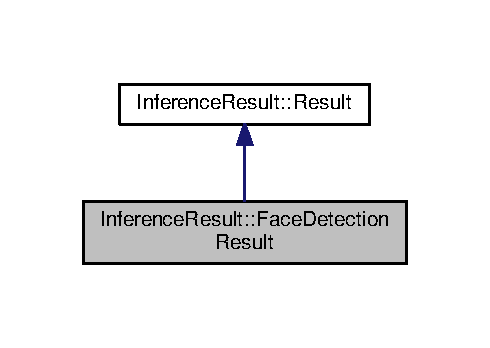
\includegraphics[width=235pt]{structInferenceResult_1_1FaceDetectionResult__inherit__graph}
\end{center}
\end{figure}


Collaboration diagram for Inference\+Result\+:\+:Face\+Detection\+Result\+:
\nopagebreak
\begin{figure}[H]
\begin{center}
\leavevmode
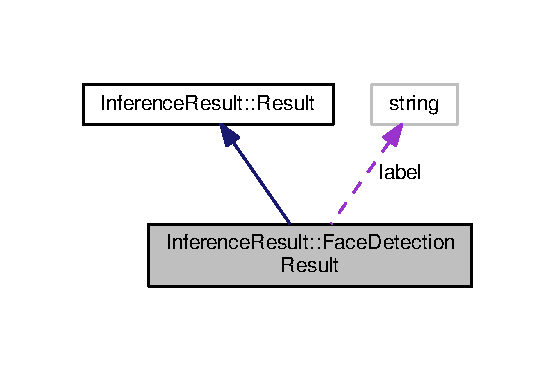
\includegraphics[width=267pt]{structInferenceResult_1_1FaceDetectionResult__coll__graph}
\end{center}
\end{figure}
\subsection*{Public Attributes}
\begin{DoxyCompactItemize}
\item 
std\+::string \hyperlink{structInferenceResult_1_1FaceDetectionResult_a395efa90912c78ac770588b57a474bd3}{label} = \char`\"{}\char`\"{}
\item 
float \hyperlink{structInferenceResult_1_1FaceDetectionResult_a7df2ce07767a0ef2c7b3ca27e9e20bc0}{confidence} = -\/1
\end{DoxyCompactItemize}


\subsection{Detailed Description}


Definition at line 17 of file data\+\_\+struct.\+h.



\subsection{Member Data Documentation}
\index{Inference\+Result\+::\+Face\+Detection\+Result@{Inference\+Result\+::\+Face\+Detection\+Result}!confidence@{confidence}}
\index{confidence@{confidence}!Inference\+Result\+::\+Face\+Detection\+Result@{Inference\+Result\+::\+Face\+Detection\+Result}}
\subsubsection[{\texorpdfstring{confidence}{confidence}}]{\setlength{\rightskip}{0pt plus 5cm}float Inference\+Result\+::\+Face\+Detection\+Result\+::confidence = -\/1}\hypertarget{structInferenceResult_1_1FaceDetectionResult_a7df2ce07767a0ef2c7b3ca27e9e20bc0}{}\label{structInferenceResult_1_1FaceDetectionResult_a7df2ce07767a0ef2c7b3ca27e9e20bc0}


Definition at line 19 of file data\+\_\+struct.\+h.

\index{Inference\+Result\+::\+Face\+Detection\+Result@{Inference\+Result\+::\+Face\+Detection\+Result}!label@{label}}
\index{label@{label}!Inference\+Result\+::\+Face\+Detection\+Result@{Inference\+Result\+::\+Face\+Detection\+Result}}
\subsubsection[{\texorpdfstring{label}{label}}]{\setlength{\rightskip}{0pt plus 5cm}std\+::string Inference\+Result\+::\+Face\+Detection\+Result\+::label = \char`\"{}\char`\"{}}\hypertarget{structInferenceResult_1_1FaceDetectionResult_a395efa90912c78ac770588b57a474bd3}{}\label{structInferenceResult_1_1FaceDetectionResult_a395efa90912c78ac770588b57a474bd3}


Definition at line 18 of file data\+\_\+struct.\+h.



The documentation for this struct was generated from the following file\+:\begin{DoxyCompactItemize}
\item 
include/openvino\+\_\+service/\hyperlink{data__struct_8h}{data\+\_\+struct.\+h}\end{DoxyCompactItemize}

\hypertarget{classFactory}{}\section{Factory Class Reference}
\label{classFactory}\index{Factory@{Factory}}


This class is a factory class that produces the derived input device class corresponding to the input string.  




{\ttfamily \#include $<$factory.\+h$>$}

\subsection*{Static Public Member Functions}
\begin{DoxyCompactItemize}
\item 
static std\+::shared\+\_\+ptr$<$ \hyperlink{classBaseInputDevice}{Base\+Input\+Device} $>$ \hyperlink{classFactory_a36585401f9a09c2d1c381546a501ea94}{make\+Input\+Device\+By\+Name} (const std\+::string \&)
\begin{DoxyCompactList}\small\item\em This function produces the derived input device class corresponding to the input string. \end{DoxyCompactList}\item 
static std\+::shared\+\_\+ptr$<$ Inference\+Engine\+::\+Inference\+Plugin $>$ \hyperlink{classFactory_a4c3731eeb49aa60626dad92f4b2cbc0d}{make\+Plugin\+By\+Name} (const std\+::string \&, const std\+::string \&, const std\+::string \&, bool)
\begin{DoxyCompactList}\small\item\em This function produces the derived inference plugin corresponding to the input string. \end{DoxyCompactList}\end{DoxyCompactItemize}


\subsection{Detailed Description}
This class is a factory class that produces the derived input device class corresponding to the input string. 

Definition at line 22 of file factory.\+h.



\subsection{Member Function Documentation}
\index{Factory@{Factory}!make\+Input\+Device\+By\+Name@{make\+Input\+Device\+By\+Name}}
\index{make\+Input\+Device\+By\+Name@{make\+Input\+Device\+By\+Name}!Factory@{Factory}}
\subsubsection[{\texorpdfstring{make\+Input\+Device\+By\+Name(const std\+::string \&)}{makeInputDeviceByName(const std::string &)}}]{\setlength{\rightskip}{0pt plus 5cm}std\+::shared\+\_\+ptr$<$ {\bf Base\+Input\+Device} $>$ Factory\+::make\+Input\+Device\+By\+Name (
\begin{DoxyParamCaption}
\item[{const std\+::string \&}]{input\+\_\+device\+\_\+name}
\end{DoxyParamCaption}
)\hspace{0.3cm}{\ttfamily [static]}}\hypertarget{classFactory_a36585401f9a09c2d1c381546a501ea94}{}\label{classFactory_a36585401f9a09c2d1c381546a501ea94}


This function produces the derived input device class corresponding to the input string. 


\begin{DoxyParams}[1]{Parameters}
\mbox{\tt in}  & {\em input} & device name, can be \hyperlink{classRealSenseCamera}{Real\+Sense\+Camera}, \hyperlink{classStandardCamera}{Standard\+Camera} or video directory \\
\hline
\end{DoxyParams}
\begin{DoxyReturn}{Returns}
the instance of derived input device referenced by a smart pointer 
\end{DoxyReturn}


Definition at line 8 of file factory.\+cpp.


\begin{DoxyCode}
8                                                                                                 \{
9   \textcolor{keywordflow}{if} (input\_device\_name == \textcolor{stringliteral}{"RealSenseCamera"}) \{
10     \textcolor{keywordflow}{return} std::make\_shared<RealSenseCamera>();
11   \} \textcolor{keywordflow}{else} \textcolor{keywordflow}{if} (input\_device\_name == \textcolor{stringliteral}{"StandardCamera"}) \{
12     \textcolor{keywordflow}{return} std::make\_shared<StandardCamera>();
13   \} \textcolor{keywordflow}{else} \{
14     \textcolor{keywordflow}{return} std::make\_shared<Video>(input\_device\_name);
15   \}
16 \}
\end{DoxyCode}
\index{Factory@{Factory}!make\+Plugin\+By\+Name@{make\+Plugin\+By\+Name}}
\index{make\+Plugin\+By\+Name@{make\+Plugin\+By\+Name}!Factory@{Factory}}
\subsubsection[{\texorpdfstring{make\+Plugin\+By\+Name(const std\+::string \&, const std\+::string \&, const std\+::string \&, bool)}{makePluginByName(const std::string &, const std::string &, const std::string &, bool)}}]{\setlength{\rightskip}{0pt plus 5cm}std\+::shared\+\_\+ptr$<$ Inference\+Plugin $>$ Factory\+::make\+Plugin\+By\+Name (
\begin{DoxyParamCaption}
\item[{const std\+::string \&}]{device\+\_\+name, }
\item[{const std\+::string \&}]{custom\+\_\+cpu\+\_\+library\+\_\+message, }
\item[{const std\+::string \&}]{custom\+\_\+cldnn\+\_\+message, }
\item[{bool}]{performance\+\_\+message}
\end{DoxyParamCaption}
)\hspace{0.3cm}{\ttfamily [static]}}\hypertarget{classFactory_a4c3731eeb49aa60626dad92f4b2cbc0d}{}\label{classFactory_a4c3731eeb49aa60626dad92f4b2cbc0d}


This function produces the derived inference plugin corresponding to the input string. 

\begin{DoxyReturn}{Returns}
the instance of derived inference plugin referenced by a smart pointer 
\end{DoxyReturn}
Printing plugin version

Load extensions for the C\+PU plugin 

Definition at line 18 of file factory.\+cpp.


\begin{DoxyCode}
21                                                                                      \{ \textcolor{comment}{//FLAGS\_pc}
22   InferencePlugin plugin =
23       PluginDispatcher(\{\textcolor{stringliteral}{"../../../lib/intel64"}, \textcolor{stringliteral}{""}\}).getPluginByDevice(
24           device\_name);
26   \hyperlink{common_8hpp_a8298b0a3bbb92311d94560e64ecfc0f1}{printPluginVersion}(plugin, std::cout);
28   \textcolor{keywordflow}{if} ((device\_name.find(\textcolor{stringliteral}{"CPU"}) != std::string::npos)) \{
29     plugin.AddExtension(std::make\_shared<Extensions::Cpu::CpuExtensions>());
30     \textcolor{keywordflow}{if} (!custom\_cpu\_library\_message.empty()) \{
31       \textcolor{comment}{// CPU(MKLDNN) extensions are loaded as a shared library and passed as a pointer to base extension}
32       \textcolor{keyword}{auto} extension\_ptr = make\_so\_pointer<MKLDNNPlugin::IMKLDNNExtension>(
33           custom\_cpu\_library\_message);
34       plugin.AddExtension(std::static\_pointer\_cast<IExtension>(extension\_ptr));
35     \}
36   \} \textcolor{keywordflow}{else} \textcolor{keywordflow}{if} (!custom\_cldnn\_message.empty()) \{
37     \textcolor{comment}{// Load Extensions for other plugins not CPU}
38     plugin.SetConfig(\{\{PluginConfigParams::KEY\_CONFIG\_FILE,
39                        custom\_cldnn\_message\}\});
40   \}
41   \textcolor{keywordflow}{if} (performance\_message) \{
42     plugin.SetConfig(\{\{PluginConfigParams::KEY\_PERF\_COUNT,
43                        PluginConfigParams::YES\}\});
44   \}
45   \textcolor{keywordflow}{return} std::make\_shared<InferencePlugin>(InferenceEngine::InferenceEnginePluginPtr(
46       plugin));
47 \}\end{DoxyCode}


The documentation for this class was generated from the following files\+:\begin{DoxyCompactItemize}
\item 
include/openvino\+\_\+service/\hyperlink{factory_8h}{factory.\+h}\item 
lib/\hyperlink{factory_8cpp}{factory.\+cpp}\end{DoxyCompactItemize}

\hypertarget{structGFLAGS__NAMESPACE_1_1FilenameFlagnameCmp}{}\section{G\+F\+L\+A\+G\+S\+\_\+\+N\+A\+M\+E\+S\+P\+A\+CE\+:\+:Filename\+Flagname\+Cmp Struct Reference}
\label{structGFLAGS__NAMESPACE_1_1FilenameFlagnameCmp}\index{G\+F\+L\+A\+G\+S\+\_\+\+N\+A\+M\+E\+S\+P\+A\+C\+E\+::\+Filename\+Flagname\+Cmp@{G\+F\+L\+A\+G\+S\+\_\+\+N\+A\+M\+E\+S\+P\+A\+C\+E\+::\+Filename\+Flagname\+Cmp}}
\subsection*{Public Member Functions}
\begin{DoxyCompactItemize}
\item 
bool \hyperlink{structGFLAGS__NAMESPACE_1_1FilenameFlagnameCmp_a8526f716b77f20a43f463f939aaf9c4b}{operator()} (const \hyperlink{structGFLAGS__NAMESPACE_1_1CommandLineFlagInfo}{Command\+Line\+Flag\+Info} \&a, const \hyperlink{structGFLAGS__NAMESPACE_1_1CommandLineFlagInfo}{Command\+Line\+Flag\+Info} \&b) const 
\end{DoxyCompactItemize}


\subsection{Detailed Description}


Definition at line 1508 of file gflags.\+cc.



\subsection{Member Function Documentation}
\index{G\+F\+L\+A\+G\+S\+\_\+\+N\+A\+M\+E\+S\+P\+A\+C\+E\+::\+Filename\+Flagname\+Cmp@{G\+F\+L\+A\+G\+S\+\_\+\+N\+A\+M\+E\+S\+P\+A\+C\+E\+::\+Filename\+Flagname\+Cmp}!operator()@{operator()}}
\index{operator()@{operator()}!G\+F\+L\+A\+G\+S\+\_\+\+N\+A\+M\+E\+S\+P\+A\+C\+E\+::\+Filename\+Flagname\+Cmp@{G\+F\+L\+A\+G\+S\+\_\+\+N\+A\+M\+E\+S\+P\+A\+C\+E\+::\+Filename\+Flagname\+Cmp}}
\subsubsection[{\texorpdfstring{operator()(const Command\+Line\+Flag\+Info \&a, const Command\+Line\+Flag\+Info \&b) const }{operator()(const CommandLineFlagInfo &a, const CommandLineFlagInfo &b) const }}]{\setlength{\rightskip}{0pt plus 5cm}bool G\+F\+L\+A\+G\+S\+\_\+\+N\+A\+M\+E\+S\+P\+A\+C\+E\+::\+Filename\+Flagname\+Cmp\+::operator() (
\begin{DoxyParamCaption}
\item[{const {\bf Command\+Line\+Flag\+Info} \&}]{a, }
\item[{const {\bf Command\+Line\+Flag\+Info} \&}]{b}
\end{DoxyParamCaption}
) const\hspace{0.3cm}{\ttfamily [inline]}}\hypertarget{structGFLAGS__NAMESPACE_1_1FilenameFlagnameCmp_a8526f716b77f20a43f463f939aaf9c4b}{}\label{structGFLAGS__NAMESPACE_1_1FilenameFlagnameCmp_a8526f716b77f20a43f463f939aaf9c4b}


Definition at line 1509 of file gflags.\+cc.


\begin{DoxyCode}
1510                                                       \{
1511     \textcolor{keywordtype}{int} cmp = strcmp(a.filename.c\_str(), b.filename.c\_str());
1512     \textcolor{keywordflow}{if} (cmp == 0)
1513       cmp = strcmp(a.name.c\_str(), b.name.c\_str());  \textcolor{comment}{// secondary sort key}
1514     \textcolor{keywordflow}{return} cmp < 0;
1515   \}
\end{DoxyCode}


The documentation for this struct was generated from the following file\+:\begin{DoxyCompactItemize}
\item 
thirdparty/gflags/src/\hyperlink{gflags_8cc}{gflags.\+cc}\end{DoxyCompactItemize}

\hypertarget{classGFLAGS__NAMESPACE_1_1FlagRegisterer}{}\section{G\+F\+L\+A\+G\+S\+\_\+\+N\+A\+M\+E\+S\+P\+A\+CE\+:\+:Flag\+Registerer Class Reference}
\label{classGFLAGS__NAMESPACE_1_1FlagRegisterer}\index{G\+F\+L\+A\+G\+S\+\_\+\+N\+A\+M\+E\+S\+P\+A\+C\+E\+::\+Flag\+Registerer@{G\+F\+L\+A\+G\+S\+\_\+\+N\+A\+M\+E\+S\+P\+A\+C\+E\+::\+Flag\+Registerer}}


{\ttfamily \#include $<$gflags.\+h$>$}

\subsection*{Public Member Functions}
\begin{DoxyCompactItemize}
\item 
{\footnotesize template$<$typename Flag\+Type $>$ }\\\hyperlink{classGFLAGS__NAMESPACE_1_1FlagRegisterer_ab3542f1059b8584757f1e9526831ebe7}{Flag\+Registerer} (const \hyperlink{CMakeCache_8txt_afe71f11dacb15682cdc012f7208e6e09}{char} $\ast$name, const \hyperlink{CMakeCache_8txt_afe71f11dacb15682cdc012f7208e6e09}{char} $\ast$help, const \hyperlink{CMakeCache_8txt_afe71f11dacb15682cdc012f7208e6e09}{char} $\ast$filename, Flag\+Type $\ast$current\+\_\+storage, Flag\+Type $\ast$defvalue\+\_\+storage)
\end{DoxyCompactItemize}


\subsection{Detailed Description}


Definition at line 432 of file gflags.\+h.



\subsection{Constructor \& Destructor Documentation}
\index{G\+F\+L\+A\+G\+S\+\_\+\+N\+A\+M\+E\+S\+P\+A\+C\+E\+::\+Flag\+Registerer@{G\+F\+L\+A\+G\+S\+\_\+\+N\+A\+M\+E\+S\+P\+A\+C\+E\+::\+Flag\+Registerer}!Flag\+Registerer@{Flag\+Registerer}}
\index{Flag\+Registerer@{Flag\+Registerer}!G\+F\+L\+A\+G\+S\+\_\+\+N\+A\+M\+E\+S\+P\+A\+C\+E\+::\+Flag\+Registerer@{G\+F\+L\+A\+G\+S\+\_\+\+N\+A\+M\+E\+S\+P\+A\+C\+E\+::\+Flag\+Registerer}}
\subsubsection[{\texorpdfstring{Flag\+Registerer(const char $\ast$name, const char $\ast$help, const char $\ast$filename, Flag\+Type $\ast$current\+\_\+storage, Flag\+Type $\ast$defvalue\+\_\+storage)}{FlagRegisterer(const char *name, const char *help, const char *filename, FlagType *current_storage, FlagType *defvalue_storage)}}]{\setlength{\rightskip}{0pt plus 5cm}template$<$typename Flag\+Type $>$ G\+F\+L\+A\+G\+S\+\_\+\+N\+A\+M\+E\+S\+P\+A\+C\+E\+::\+Flag\+Registerer\+::\+Flag\+Registerer (
\begin{DoxyParamCaption}
\item[{const {\bf char} $\ast$}]{name, }
\item[{const {\bf char} $\ast$}]{help, }
\item[{const {\bf char} $\ast$}]{filename, }
\item[{Flag\+Type $\ast$}]{current\+\_\+storage, }
\item[{Flag\+Type $\ast$}]{defvalue\+\_\+storage}
\end{DoxyParamCaption}
)}\hypertarget{classGFLAGS__NAMESPACE_1_1FlagRegisterer_ab3542f1059b8584757f1e9526831ebe7}{}\label{classGFLAGS__NAMESPACE_1_1FlagRegisterer_ab3542f1059b8584757f1e9526831ebe7}


Definition at line 1473 of file gflags.\+cc.


\begin{DoxyCode}
1477                                                            \{
1478   FlagValue* \textcolor{keyword}{const} current = \textcolor{keyword}{new} FlagValue(current\_storage, \textcolor{keyword}{false});
1479   FlagValue* \textcolor{keyword}{const} defvalue = \textcolor{keyword}{new} FlagValue(defvalue\_storage, \textcolor{keyword}{false});
1480   RegisterCommandLineFlag(name, help, filename, current, defvalue);
1481 \}
\end{DoxyCode}


The documentation for this class was generated from the following files\+:\begin{DoxyCompactItemize}
\item 
cmake-\/build-\/debug/thirdparty/gflags/include/gflags/\hyperlink{gflags_8h}{gflags.\+h}\item 
thirdparty/gflags/src/\hyperlink{gflags_8cc}{gflags.\+cc}\end{DoxyCompactItemize}

\hypertarget{classGFLAGS__NAMESPACE_1_1FlagSaver}{}\section{G\+F\+L\+A\+G\+S\+\_\+\+N\+A\+M\+E\+S\+P\+A\+CE\+:\+:Flag\+Saver Class Reference}
\label{classGFLAGS__NAMESPACE_1_1FlagSaver}\index{G\+F\+L\+A\+G\+S\+\_\+\+N\+A\+M\+E\+S\+P\+A\+C\+E\+::\+Flag\+Saver@{G\+F\+L\+A\+G\+S\+\_\+\+N\+A\+M\+E\+S\+P\+A\+C\+E\+::\+Flag\+Saver}}


{\ttfamily \#include $<$gflags.\+h$>$}

\subsection*{Public Member Functions}
\begin{DoxyCompactItemize}
\item 
\hyperlink{classGFLAGS__NAMESPACE_1_1FlagSaver_a7b459e22bdcf8adcf7a22fbeb321cc3d}{Flag\+Saver} ()
\item 
\hyperlink{classGFLAGS__NAMESPACE_1_1FlagSaver_a9af1aa996c4929d6ae4e8fe9462bdb9d}{$\sim$\+Flag\+Saver} ()
\end{DoxyCompactItemize}


\subsection{Detailed Description}


Definition at line 278 of file gflags.\+h.



\subsection{Constructor \& Destructor Documentation}
\index{G\+F\+L\+A\+G\+S\+\_\+\+N\+A\+M\+E\+S\+P\+A\+C\+E\+::\+Flag\+Saver@{G\+F\+L\+A\+G\+S\+\_\+\+N\+A\+M\+E\+S\+P\+A\+C\+E\+::\+Flag\+Saver}!Flag\+Saver@{Flag\+Saver}}
\index{Flag\+Saver@{Flag\+Saver}!G\+F\+L\+A\+G\+S\+\_\+\+N\+A\+M\+E\+S\+P\+A\+C\+E\+::\+Flag\+Saver@{G\+F\+L\+A\+G\+S\+\_\+\+N\+A\+M\+E\+S\+P\+A\+C\+E\+::\+Flag\+Saver}}
\subsubsection[{\texorpdfstring{Flag\+Saver()}{FlagSaver()}}]{\setlength{\rightskip}{0pt plus 5cm}G\+F\+L\+A\+G\+S\+\_\+\+N\+A\+M\+E\+S\+P\+A\+C\+E\+::\+Flag\+Saver\+::\+Flag\+Saver (
\begin{DoxyParamCaption}
{}
\end{DoxyParamCaption}
)}\hypertarget{classGFLAGS__NAMESPACE_1_1FlagSaver_a7b459e22bdcf8adcf7a22fbeb321cc3d}{}\label{classGFLAGS__NAMESPACE_1_1FlagSaver_a7b459e22bdcf8adcf7a22fbeb321cc3d}


Definition at line 1762 of file gflags.\+cc.


\begin{DoxyCode}
1763     : impl\_(\textcolor{keyword}{new} FlagSaverImpl(FlagRegistry::GlobalRegistry())) \{
1764   impl\_->\hyperlink{classGFLAGS__NAMESPACE_1_1FlagSaverImpl_a1837d4337e8093b087a862b2f7e55f1e}{SaveFromRegistry}();
1765 \}
\end{DoxyCode}
\index{G\+F\+L\+A\+G\+S\+\_\+\+N\+A\+M\+E\+S\+P\+A\+C\+E\+::\+Flag\+Saver@{G\+F\+L\+A\+G\+S\+\_\+\+N\+A\+M\+E\+S\+P\+A\+C\+E\+::\+Flag\+Saver}!````~Flag\+Saver@{$\sim$\+Flag\+Saver}}
\index{````~Flag\+Saver@{$\sim$\+Flag\+Saver}!G\+F\+L\+A\+G\+S\+\_\+\+N\+A\+M\+E\+S\+P\+A\+C\+E\+::\+Flag\+Saver@{G\+F\+L\+A\+G\+S\+\_\+\+N\+A\+M\+E\+S\+P\+A\+C\+E\+::\+Flag\+Saver}}
\subsubsection[{\texorpdfstring{$\sim$\+Flag\+Saver()}{~FlagSaver()}}]{\setlength{\rightskip}{0pt plus 5cm}G\+F\+L\+A\+G\+S\+\_\+\+N\+A\+M\+E\+S\+P\+A\+C\+E\+::\+Flag\+Saver\+::$\sim$\+Flag\+Saver (
\begin{DoxyParamCaption}
{}
\end{DoxyParamCaption}
)}\hypertarget{classGFLAGS__NAMESPACE_1_1FlagSaver_a9af1aa996c4929d6ae4e8fe9462bdb9d}{}\label{classGFLAGS__NAMESPACE_1_1FlagSaver_a9af1aa996c4929d6ae4e8fe9462bdb9d}


Definition at line 1767 of file gflags.\+cc.


\begin{DoxyCode}
1767                       \{
1768   impl\_->\hyperlink{classGFLAGS__NAMESPACE_1_1FlagSaverImpl_aff23b2a8c68020ee000c5083d4ed9c75}{RestoreToRegistry}();
1769   \textcolor{keyword}{delete} impl\_;
1770 \}
\end{DoxyCode}


The documentation for this class was generated from the following files\+:\begin{DoxyCompactItemize}
\item 
cmake-\/build-\/debug/thirdparty/gflags/include/gflags/\hyperlink{gflags_8h}{gflags.\+h}\item 
thirdparty/gflags/src/\hyperlink{gflags_8cc}{gflags.\+cc}\end{DoxyCompactItemize}

\hypertarget{classGFLAGS__NAMESPACE_1_1FlagSaverImpl}{}\section{G\+F\+L\+A\+G\+S\+\_\+\+N\+A\+M\+E\+S\+P\+A\+CE\+:\+:Flag\+Saver\+Impl Class Reference}
\label{classGFLAGS__NAMESPACE_1_1FlagSaverImpl}\index{G\+F\+L\+A\+G\+S\+\_\+\+N\+A\+M\+E\+S\+P\+A\+C\+E\+::\+Flag\+Saver\+Impl@{G\+F\+L\+A\+G\+S\+\_\+\+N\+A\+M\+E\+S\+P\+A\+C\+E\+::\+Flag\+Saver\+Impl}}
\subsection*{Public Member Functions}
\begin{DoxyCompactItemize}
\item 
\hyperlink{classGFLAGS__NAMESPACE_1_1FlagSaverImpl_aea68c700bea03690d22019e00aa9c59a}{Flag\+Saver\+Impl} (Flag\+Registry $\ast$main\+\_\+registry)
\item 
\hyperlink{classGFLAGS__NAMESPACE_1_1FlagSaverImpl_a479a7316da81d6d3767b2940118071d8}{$\sim$\+Flag\+Saver\+Impl} ()
\item 
void \hyperlink{classGFLAGS__NAMESPACE_1_1FlagSaverImpl_a1837d4337e8093b087a862b2f7e55f1e}{Save\+From\+Registry} ()
\item 
void \hyperlink{classGFLAGS__NAMESPACE_1_1FlagSaverImpl_aff23b2a8c68020ee000c5083d4ed9c75}{Restore\+To\+Registry} ()
\end{DoxyCompactItemize}


\subsection{Detailed Description}


Definition at line 1707 of file gflags.\+cc.



\subsection{Constructor \& Destructor Documentation}
\index{G\+F\+L\+A\+G\+S\+\_\+\+N\+A\+M\+E\+S\+P\+A\+C\+E\+::\+Flag\+Saver\+Impl@{G\+F\+L\+A\+G\+S\+\_\+\+N\+A\+M\+E\+S\+P\+A\+C\+E\+::\+Flag\+Saver\+Impl}!Flag\+Saver\+Impl@{Flag\+Saver\+Impl}}
\index{Flag\+Saver\+Impl@{Flag\+Saver\+Impl}!G\+F\+L\+A\+G\+S\+\_\+\+N\+A\+M\+E\+S\+P\+A\+C\+E\+::\+Flag\+Saver\+Impl@{G\+F\+L\+A\+G\+S\+\_\+\+N\+A\+M\+E\+S\+P\+A\+C\+E\+::\+Flag\+Saver\+Impl}}
\subsubsection[{\texorpdfstring{Flag\+Saver\+Impl(\+Flag\+Registry $\ast$main\+\_\+registry)}{FlagSaverImpl(FlagRegistry *main_registry)}}]{\setlength{\rightskip}{0pt plus 5cm}G\+F\+L\+A\+G\+S\+\_\+\+N\+A\+M\+E\+S\+P\+A\+C\+E\+::\+Flag\+Saver\+Impl\+::\+Flag\+Saver\+Impl (
\begin{DoxyParamCaption}
\item[{Flag\+Registry $\ast$}]{main\+\_\+registry}
\end{DoxyParamCaption}
)\hspace{0.3cm}{\ttfamily [inline]}, {\ttfamily [explicit]}}\hypertarget{classGFLAGS__NAMESPACE_1_1FlagSaverImpl_aea68c700bea03690d22019e00aa9c59a}{}\label{classGFLAGS__NAMESPACE_1_1FlagSaverImpl_aea68c700bea03690d22019e00aa9c59a}


Definition at line 1710 of file gflags.\+cc.


\begin{DoxyCode}
1711       : main\_registry\_(main\_registry) \{ \}
\end{DoxyCode}
\index{G\+F\+L\+A\+G\+S\+\_\+\+N\+A\+M\+E\+S\+P\+A\+C\+E\+::\+Flag\+Saver\+Impl@{G\+F\+L\+A\+G\+S\+\_\+\+N\+A\+M\+E\+S\+P\+A\+C\+E\+::\+Flag\+Saver\+Impl}!````~Flag\+Saver\+Impl@{$\sim$\+Flag\+Saver\+Impl}}
\index{````~Flag\+Saver\+Impl@{$\sim$\+Flag\+Saver\+Impl}!G\+F\+L\+A\+G\+S\+\_\+\+N\+A\+M\+E\+S\+P\+A\+C\+E\+::\+Flag\+Saver\+Impl@{G\+F\+L\+A\+G\+S\+\_\+\+N\+A\+M\+E\+S\+P\+A\+C\+E\+::\+Flag\+Saver\+Impl}}
\subsubsection[{\texorpdfstring{$\sim$\+Flag\+Saver\+Impl()}{~FlagSaverImpl()}}]{\setlength{\rightskip}{0pt plus 5cm}G\+F\+L\+A\+G\+S\+\_\+\+N\+A\+M\+E\+S\+P\+A\+C\+E\+::\+Flag\+Saver\+Impl\+::$\sim$\+Flag\+Saver\+Impl (
\begin{DoxyParamCaption}
{}
\end{DoxyParamCaption}
)\hspace{0.3cm}{\ttfamily [inline]}}\hypertarget{classGFLAGS__NAMESPACE_1_1FlagSaverImpl_a479a7316da81d6d3767b2940118071d8}{}\label{classGFLAGS__NAMESPACE_1_1FlagSaverImpl_a479a7316da81d6d3767b2940118071d8}


Definition at line 1712 of file gflags.\+cc.


\begin{DoxyCode}
1712                    \{
1713     \textcolor{comment}{// reclaim memory from each of our CommandLineFlags}
1714     vector<CommandLineFlag*>::const\_iterator it;
1715     \textcolor{keywordflow}{for} (it = backup\_registry\_.begin(); it != backup\_registry\_.end(); ++it)
1716       \textcolor{keyword}{delete} *it;
1717   \}
\end{DoxyCode}


\subsection{Member Function Documentation}
\index{G\+F\+L\+A\+G\+S\+\_\+\+N\+A\+M\+E\+S\+P\+A\+C\+E\+::\+Flag\+Saver\+Impl@{G\+F\+L\+A\+G\+S\+\_\+\+N\+A\+M\+E\+S\+P\+A\+C\+E\+::\+Flag\+Saver\+Impl}!Restore\+To\+Registry@{Restore\+To\+Registry}}
\index{Restore\+To\+Registry@{Restore\+To\+Registry}!G\+F\+L\+A\+G\+S\+\_\+\+N\+A\+M\+E\+S\+P\+A\+C\+E\+::\+Flag\+Saver\+Impl@{G\+F\+L\+A\+G\+S\+\_\+\+N\+A\+M\+E\+S\+P\+A\+C\+E\+::\+Flag\+Saver\+Impl}}
\subsubsection[{\texorpdfstring{Restore\+To\+Registry()}{RestoreToRegistry()}}]{\setlength{\rightskip}{0pt plus 5cm}void G\+F\+L\+A\+G\+S\+\_\+\+N\+A\+M\+E\+S\+P\+A\+C\+E\+::\+Flag\+Saver\+Impl\+::\+Restore\+To\+Registry (
\begin{DoxyParamCaption}
{}
\end{DoxyParamCaption}
)\hspace{0.3cm}{\ttfamily [inline]}}\hypertarget{classGFLAGS__NAMESPACE_1_1FlagSaverImpl_aff23b2a8c68020ee000c5083d4ed9c75}{}\label{classGFLAGS__NAMESPACE_1_1FlagSaverImpl_aff23b2a8c68020ee000c5083d4ed9c75}


Definition at line 1743 of file gflags.\+cc.


\begin{DoxyCode}
1743                            \{
1744     FlagRegistryLock frl(main\_registry\_);
1745     vector<CommandLineFlag*>::const\_iterator it;
1746     \textcolor{keywordflow}{for} (it = backup\_registry\_.begin(); it != backup\_registry\_.end(); ++it) \{
1747       CommandLineFlag* \hyperlink{CMakeCCompilerId_8c_a0ddf1224851353fc92bfbff6f499fa97}{main} = main\_registry\_->FindFlagLocked((*it)->name());
1748       \textcolor{keywordflow}{if} (main != NULL) \{       \textcolor{comment}{// if NULL, flag got deleted from registry(!)}
1749         main->CopyFrom(**it);
1750       \}
1751     \}
1752   \}
\end{DoxyCode}
\index{G\+F\+L\+A\+G\+S\+\_\+\+N\+A\+M\+E\+S\+P\+A\+C\+E\+::\+Flag\+Saver\+Impl@{G\+F\+L\+A\+G\+S\+\_\+\+N\+A\+M\+E\+S\+P\+A\+C\+E\+::\+Flag\+Saver\+Impl}!Save\+From\+Registry@{Save\+From\+Registry}}
\index{Save\+From\+Registry@{Save\+From\+Registry}!G\+F\+L\+A\+G\+S\+\_\+\+N\+A\+M\+E\+S\+P\+A\+C\+E\+::\+Flag\+Saver\+Impl@{G\+F\+L\+A\+G\+S\+\_\+\+N\+A\+M\+E\+S\+P\+A\+C\+E\+::\+Flag\+Saver\+Impl}}
\subsubsection[{\texorpdfstring{Save\+From\+Registry()}{SaveFromRegistry()}}]{\setlength{\rightskip}{0pt plus 5cm}void G\+F\+L\+A\+G\+S\+\_\+\+N\+A\+M\+E\+S\+P\+A\+C\+E\+::\+Flag\+Saver\+Impl\+::\+Save\+From\+Registry (
\begin{DoxyParamCaption}
{}
\end{DoxyParamCaption}
)\hspace{0.3cm}{\ttfamily [inline]}}\hypertarget{classGFLAGS__NAMESPACE_1_1FlagSaverImpl_a1837d4337e8093b087a862b2f7e55f1e}{}\label{classGFLAGS__NAMESPACE_1_1FlagSaverImpl_a1837d4337e8093b087a862b2f7e55f1e}


Definition at line 1722 of file gflags.\+cc.


\begin{DoxyCode}
1722                           \{
1723     FlagRegistryLock frl(main\_registry\_);
1724     assert(backup\_registry\_.empty());   \textcolor{comment}{// call only once!}
1725     \textcolor{keywordflow}{for} (FlagRegistry::FlagConstIterator it = main\_registry\_->flags\_.begin();
1726          it != main\_registry\_->flags\_.end();
1727          ++it) \{
1728       \textcolor{keyword}{const} CommandLineFlag* \hyperlink{CMakeCCompilerId_8c_a0ddf1224851353fc92bfbff6f499fa97}{main} = it->second;
1729       \textcolor{comment}{// Sets up all the const variables in backup correctly}
1730       CommandLineFlag* backup = \textcolor{keyword}{new} CommandLineFlag(
1731           main->name(), main->help(), main->filename(),
1732           main->current\_->New(), main->defvalue\_->New());
1733       \textcolor{comment}{// Sets up all the non-const variables in backup correctly}
1734       backup->CopyFrom(*main);
1735       backup\_registry\_.push\_back(backup);   \textcolor{comment}{// add it to a convenient list}
1736     \}
1737   \}
\end{DoxyCode}


The documentation for this class was generated from the following file\+:\begin{DoxyCompactItemize}
\item 
thirdparty/gflags/src/\hyperlink{gflags_8cc}{gflags.\+cc}\end{DoxyCompactItemize}

\hypertarget{classInferenceEngine_1_1Extensions_1_1Cpu_1_1GRNImpl}{}\section{Inference\+Engine\+:\+:Extensions\+:\+:Cpu\+:\+:G\+R\+N\+Impl Class Reference}
\label{classInferenceEngine_1_1Extensions_1_1Cpu_1_1GRNImpl}\index{Inference\+Engine\+::\+Extensions\+::\+Cpu\+::\+G\+R\+N\+Impl@{Inference\+Engine\+::\+Extensions\+::\+Cpu\+::\+G\+R\+N\+Impl}}


Inheritance diagram for Inference\+Engine\+:\+:Extensions\+:\+:Cpu\+:\+:G\+R\+N\+Impl\+:
\nopagebreak
\begin{figure}[H]
\begin{center}
\leavevmode
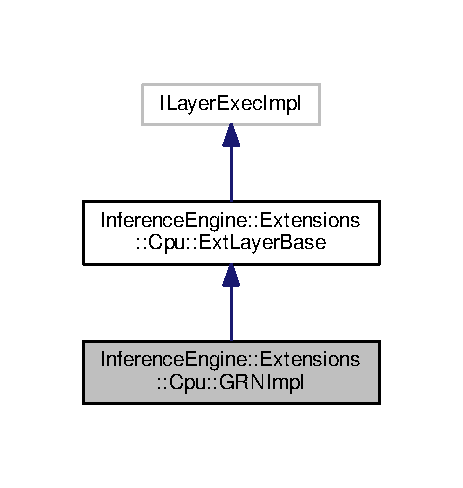
\includegraphics[width=222pt]{classInferenceEngine_1_1Extensions_1_1Cpu_1_1GRNImpl__inherit__graph}
\end{center}
\end{figure}


Collaboration diagram for Inference\+Engine\+:\+:Extensions\+:\+:Cpu\+:\+:G\+R\+N\+Impl\+:
\nopagebreak
\begin{figure}[H]
\begin{center}
\leavevmode
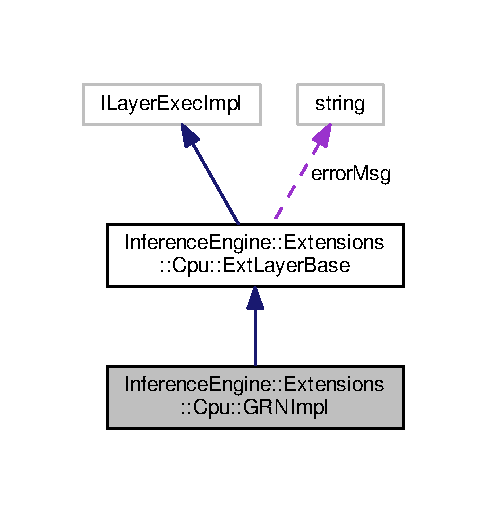
\includegraphics[width=234pt]{classInferenceEngine_1_1Extensions_1_1Cpu_1_1GRNImpl__coll__graph}
\end{center}
\end{figure}
\subsection*{Public Member Functions}
\begin{DoxyCompactItemize}
\item 
\hyperlink{classInferenceEngine_1_1Extensions_1_1Cpu_1_1GRNImpl_ad07b1fb8ba936455acee2baa4725a11a}{G\+R\+N\+Impl} (const C\+N\+N\+Layer $\ast$layer)
\item 
Status\+Code \hyperlink{classInferenceEngine_1_1Extensions_1_1Cpu_1_1GRNImpl_a1f1d69a96755619c12e02d93666f4ae6}{execute} (std\+::vector$<$ Blob\+::\+Ptr $>$ \&inputs, std\+::vector$<$ Blob\+::\+Ptr $>$ \&outputs, Response\+Desc $\ast$resp) noexceptoverride
\end{DoxyCompactItemize}
\subsection*{Additional Inherited Members}


\subsection{Detailed Description}


Definition at line 28 of file ext\+\_\+grn.\+cpp.



\subsection{Constructor \& Destructor Documentation}
\index{Inference\+Engine\+::\+Extensions\+::\+Cpu\+::\+G\+R\+N\+Impl@{Inference\+Engine\+::\+Extensions\+::\+Cpu\+::\+G\+R\+N\+Impl}!G\+R\+N\+Impl@{G\+R\+N\+Impl}}
\index{G\+R\+N\+Impl@{G\+R\+N\+Impl}!Inference\+Engine\+::\+Extensions\+::\+Cpu\+::\+G\+R\+N\+Impl@{Inference\+Engine\+::\+Extensions\+::\+Cpu\+::\+G\+R\+N\+Impl}}
\subsubsection[{\texorpdfstring{G\+R\+N\+Impl(const C\+N\+N\+Layer $\ast$layer)}{GRNImpl(const CNNLayer *layer)}}]{\setlength{\rightskip}{0pt plus 5cm}Inference\+Engine\+::\+Extensions\+::\+Cpu\+::\+G\+R\+N\+Impl\+::\+G\+R\+N\+Impl (
\begin{DoxyParamCaption}
\item[{const C\+N\+N\+Layer $\ast$}]{layer}
\end{DoxyParamCaption}
)\hspace{0.3cm}{\ttfamily [inline]}, {\ttfamily [explicit]}}\hypertarget{classInferenceEngine_1_1Extensions_1_1Cpu_1_1GRNImpl_ad07b1fb8ba936455acee2baa4725a11a}{}\label{classInferenceEngine_1_1Extensions_1_1Cpu_1_1GRNImpl_ad07b1fb8ba936455acee2baa4725a11a}


Definition at line 30 of file ext\+\_\+grn.\+cpp.


\begin{DoxyCode}
30                                            : \hyperlink{classInferenceEngine_1_1Extensions_1_1Cpu_1_1ExtLayerBase_affff0e8263ca26852ccf71d299d7b06a}{ExtLayerBase}(layer) \{
31         \textcolor{keywordflow}{try} \{
32             \textcolor{keywordflow}{if} (\hyperlink{classInferenceEngine_1_1Extensions_1_1Cpu_1_1ExtLayerBase_a1074cdccacb9e9ca6eec01bbc2f7ca4a}{cnnLayer}.insData.size() != 1 || \hyperlink{classInferenceEngine_1_1Extensions_1_1Cpu_1_1ExtLayerBase_a1074cdccacb9e9ca6eec01bbc2f7ca4a}{cnnLayer}.outData.empty())
33                 THROW\_IE\_EXCEPTION << \textcolor{stringliteral}{"Incorrect number of input/output edges!"};
34 
35             bias = \hyperlink{classInferenceEngine_1_1Extensions_1_1Cpu_1_1ExtLayerBase_a1074cdccacb9e9ca6eec01bbc2f7ca4a}{cnnLayer}.GetParamAsFloat(\textcolor{stringliteral}{"bias"});
36 
37             \hyperlink{classInferenceEngine_1_1Extensions_1_1Cpu_1_1ExtLayerBase_a0ac7a6632e95b9500d5246b05b4b0bfa}{addConfig}(\{\{\hyperlink{classInferenceEngine_1_1Extensions_1_1Cpu_1_1ExtLayerBase_a1258a8d209e0249e0b1717618352ddfba446687ea2db1ada75be5ed053be77f59}{ConfLayout::PLN}, \textcolor{keyword}{false}, 0\}\}, \{\{
      \hyperlink{classInferenceEngine_1_1Extensions_1_1Cpu_1_1ExtLayerBase_a1258a8d209e0249e0b1717618352ddfba446687ea2db1ada75be5ed053be77f59}{ConfLayout::PLN}, \textcolor{keyword}{false}, 0\}\});
38         \} \textcolor{keywordflow}{catch} (InferenceEngine::details::InferenceEngineException &ex) \{
39             \hyperlink{classInferenceEngine_1_1Extensions_1_1Cpu_1_1ExtLayerBase_abc78e9b5a79fa339ffd831a5318f71f7}{errorMsg} = ex.what();
40         \}
41     \}
\end{DoxyCode}


\subsection{Member Function Documentation}
\index{Inference\+Engine\+::\+Extensions\+::\+Cpu\+::\+G\+R\+N\+Impl@{Inference\+Engine\+::\+Extensions\+::\+Cpu\+::\+G\+R\+N\+Impl}!execute@{execute}}
\index{execute@{execute}!Inference\+Engine\+::\+Extensions\+::\+Cpu\+::\+G\+R\+N\+Impl@{Inference\+Engine\+::\+Extensions\+::\+Cpu\+::\+G\+R\+N\+Impl}}
\subsubsection[{\texorpdfstring{execute(std\+::vector$<$ Blob\+::\+Ptr $>$ \&inputs, std\+::vector$<$ Blob\+::\+Ptr $>$ \&outputs, Response\+Desc $\ast$resp) noexceptoverride}{execute(std::vector< Blob::Ptr > &inputs, std::vector< Blob::Ptr > &outputs, ResponseDesc *resp) noexceptoverride}}]{\setlength{\rightskip}{0pt plus 5cm}Status\+Code Inference\+Engine\+::\+Extensions\+::\+Cpu\+::\+G\+R\+N\+Impl\+::execute (
\begin{DoxyParamCaption}
\item[{std\+::vector$<$ Blob\+::\+Ptr $>$ \&}]{inputs, }
\item[{std\+::vector$<$ Blob\+::\+Ptr $>$ \&}]{outputs, }
\item[{Response\+Desc $\ast$}]{resp}
\end{DoxyParamCaption}
)\hspace{0.3cm}{\ttfamily [inline]}, {\ttfamily [override]}, {\ttfamily [noexcept]}}\hypertarget{classInferenceEngine_1_1Extensions_1_1Cpu_1_1GRNImpl_a1f1d69a96755619c12e02d93666f4ae6}{}\label{classInferenceEngine_1_1Extensions_1_1Cpu_1_1GRNImpl_a1f1d69a96755619c12e02d93666f4ae6}


Definition at line 43 of file ext\+\_\+grn.\+cpp.


\begin{DoxyCode}
44                                                              \{
45         \textcolor{keywordtype}{float}* src\_data = inputs[0]->buffer();
46         \textcolor{keywordtype}{float}* dst\_data = outputs[0]->buffer();
47 
48         SizeVector dims = inputs[0]->getTensorDesc().getDims();
49 
50         \textcolor{keywordtype}{int} N = \textcolor{keyword}{static\_cast<}\textcolor{keywordtype}{int}\textcolor{keyword}{>}((dims.size() > 0) ? dims[0] : 1);
51         \textcolor{keywordtype}{int} C = \textcolor{keyword}{static\_cast<}\textcolor{keywordtype}{int}\textcolor{keyword}{>}((dims.size() > 1) ? dims[1] : 1);
52         \textcolor{keywordtype}{int} H = \textcolor{keyword}{static\_cast<}\textcolor{keywordtype}{int}\textcolor{keyword}{>}((dims.size() > 2) ? dims[2] : 1);
53         \textcolor{keywordtype}{int} W = \textcolor{keyword}{static\_cast<}\textcolor{keywordtype}{int}\textcolor{keyword}{>}((dims.size() > 3) ? dims[3] : 1);
54 
55 \textcolor{preprocessor}{#if \_MSC\_VER && !\_\_INTEL\_COMPILER}
56 \textcolor{preprocessor}{        #pragma omp parallel for schedule(static)}
57 \textcolor{preprocessor}{#else}
58 \textcolor{preprocessor}{        #pragma omp parallel for collapse(3) schedule(static)}
59 \textcolor{preprocessor}{#endif}
60         \textcolor{keywordflow}{for} (\textcolor{keywordtype}{int} b = 0; b < N; b++) \{
61             \textcolor{keywordflow}{for} (\textcolor{keywordtype}{int} h = 0; h < H; h++) \{
62                 \textcolor{keywordflow}{for} (\textcolor{keywordtype}{int} w = 0; w < W; w++) \{
63                     \textcolor{keywordtype}{double} variance = 0;
64                     \textcolor{keywordflow}{for} (\textcolor{keywordtype}{int} \hyperlink{CMakeCache_8txt_aac1d6a1710812201527c735f7c6afbaa}{c} = 0; \hyperlink{CMakeCache_8txt_aac1d6a1710812201527c735f7c6afbaa}{c} < C; \hyperlink{CMakeCache_8txt_aac1d6a1710812201527c735f7c6afbaa}{c}++) \{
65                         variance += std::pow(src\_data[b*C*H*W + \hyperlink{CMakeCache_8txt_aac1d6a1710812201527c735f7c6afbaa}{c}*H*W + h*W + w], 2);
66                     \}
67                     variance = std::pow(variance + bias, 0.5f);
68                     \textcolor{keywordflow}{for} (\textcolor{keywordtype}{int} \hyperlink{CMakeCache_8txt_aac1d6a1710812201527c735f7c6afbaa}{c} = 0; \hyperlink{CMakeCache_8txt_aac1d6a1710812201527c735f7c6afbaa}{c} < C; \hyperlink{CMakeCache_8txt_aac1d6a1710812201527c735f7c6afbaa}{c}++) \{
69                         dst\_data[b*C*H*W + \hyperlink{CMakeCache_8txt_aac1d6a1710812201527c735f7c6afbaa}{c}*H*W + h*W + w] = src\_data[b*C*H*W + 
      \hyperlink{CMakeCache_8txt_aac1d6a1710812201527c735f7c6afbaa}{c}*H*W + h*W + w] / variance;
70                     \}
71                 \}
72             \}
73         \}
74         \textcolor{keywordflow}{return} OK;
75     \}
\end{DoxyCode}


The documentation for this class was generated from the following file\+:\begin{DoxyCompactItemize}
\item 
thirdparty/extension/\hyperlink{ext__grn_8cpp}{ext\+\_\+grn.\+cpp}\end{DoxyCompactItemize}

\hypertarget{classopenvino__service_1_1HeadPoseDetection}{}\section{openvino\+\_\+service\+:\+:Head\+Pose\+Detection Class Reference}
\label{classopenvino__service_1_1HeadPoseDetection}\index{openvino\+\_\+service\+::\+Head\+Pose\+Detection@{openvino\+\_\+service\+::\+Head\+Pose\+Detection}}


{\ttfamily \#include $<$head\+\_\+pose\+\_\+recognition.\+h$>$}



Inheritance diagram for openvino\+\_\+service\+:\+:Head\+Pose\+Detection\+:
\nopagebreak
\begin{figure}[H]
\begin{center}
\leavevmode
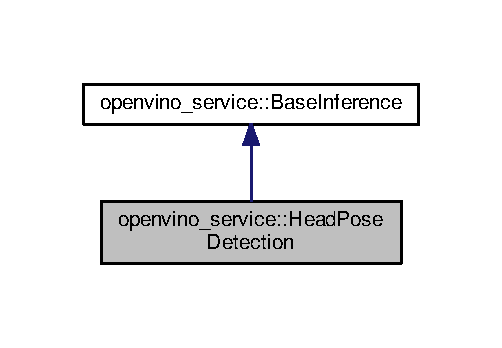
\includegraphics[width=241pt]{classopenvino__service_1_1HeadPoseDetection__inherit__graph}
\end{center}
\end{figure}


Collaboration diagram for openvino\+\_\+service\+:\+:Head\+Pose\+Detection\+:
\nopagebreak
\begin{figure}[H]
\begin{center}
\leavevmode
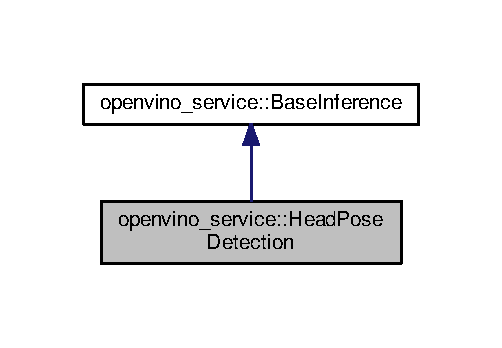
\includegraphics[width=241pt]{classopenvino__service_1_1HeadPoseDetection__coll__graph}
\end{center}
\end{figure}
\subsection*{Public Types}
\begin{DoxyCompactItemize}
\item 
using \hyperlink{classopenvino__service_1_1HeadPoseDetection_a2974bab186f80414217225d2f1fb6de9}{Result} = \hyperlink{structInferenceResult_1_1HeadPoseResult}{Inference\+Result\+::\+Head\+Pose\+Result}
\end{DoxyCompactItemize}
\subsection*{Public Member Functions}
\begin{DoxyCompactItemize}
\item 
\hyperlink{classopenvino__service_1_1HeadPoseDetection_abc430e5f6ae895d6bb4e34187f5fcd42}{Head\+Pose\+Detection} ()
\item 
\hyperlink{classopenvino__service_1_1HeadPoseDetection_a9fcba4b94c60854b54fcdde3fa839edd}{$\sim$\+Head\+Pose\+Detection} () override
\item 
void \hyperlink{classopenvino__service_1_1HeadPoseDetection_a8c4aa2573675e9fa4276b713d67b94eb}{load\+Network} (std\+::shared\+\_\+ptr$<$ \hyperlink{classValidatedHeadPoseNetwork}{Validated\+Head\+Pose\+Network} $>$)
\item 
bool \hyperlink{classopenvino__service_1_1HeadPoseDetection_a122807cd1add8980b21c76a9b9f1f300}{enqueue} (const cv\+::\+Mat \&frame, const cv\+::\+Rect \&) override
\begin{DoxyCompactList}\small\item\em Enqueue a frame to this class. The frame will be buffered but not infered yet. \end{DoxyCompactList}\item 
bool \hyperlink{classopenvino__service_1_1HeadPoseDetection_ac985e9d741eeacdd75467f9929aaf0f7}{submit\+Request} () override
\begin{DoxyCompactList}\small\item\em Start inference for all buffered frames. \end{DoxyCompactList}\item 
bool \hyperlink{classopenvino__service_1_1HeadPoseDetection_a252bfae15900a6d5936e742a418fe684}{fetch\+Results} () override
\begin{DoxyCompactList}\small\item\em This function will fetch the results of the previous inference and stores the results in a result buffer array. All buffered frames will be cleared. \end{DoxyCompactList}\item 
void \hyperlink{classopenvino__service_1_1HeadPoseDetection_a32d824cdba6b6655a1280b1c01bce13e}{accepts} (std\+::shared\+\_\+ptr$<$ \hyperlink{classBaseOutput}{Base\+Output} $>$ output\+\_\+visitor) override
\begin{DoxyCompactList}\small\item\em Accepts an Output instance for result process. This function is used for visitor pattern. \end{DoxyCompactList}\item 
const \hyperlink{CMakeCache_8txt_a79a3d8790b2588b09777910863574e09}{int} \hyperlink{classopenvino__service_1_1HeadPoseDetection_a12cda8df1f3bdb640a27c17d36bb18ae}{get\+Results\+Length} () const override
\begin{DoxyCompactList}\small\item\em Get the length of the buffer result array. \end{DoxyCompactList}\item 
const \hyperlink{structInferenceResult_1_1Result}{Inference\+Result\+::\+Result} \hyperlink{classopenvino__service_1_1HeadPoseDetection_a2e85b9f74da265a413fd634106514ea9}{get\+Location\+Result} (\hyperlink{CMakeCache_8txt_a79a3d8790b2588b09777910863574e09}{int} idx) const override
\begin{DoxyCompactList}\small\item\em Get the location of result with respect to the frame generated by the input device. \end{DoxyCompactList}\item 
const std\+::string \hyperlink{classopenvino__service_1_1HeadPoseDetection_ae9333037746d10b2aef1cd1d4ec0cf91}{get\+Name} () const override
\begin{DoxyCompactList}\small\item\em Get the name of the Inference instance. \end{DoxyCompactList}\end{DoxyCompactItemize}
\subsection*{Additional Inherited Members}


\subsection{Detailed Description}


Definition at line 21 of file head\+\_\+pose\+\_\+recognition.\+h.



\subsection{Member Typedef Documentation}
\index{openvino\+\_\+service\+::\+Head\+Pose\+Detection@{openvino\+\_\+service\+::\+Head\+Pose\+Detection}!Result@{Result}}
\index{Result@{Result}!openvino\+\_\+service\+::\+Head\+Pose\+Detection@{openvino\+\_\+service\+::\+Head\+Pose\+Detection}}
\subsubsection[{\texorpdfstring{Result}{Result}}]{\setlength{\rightskip}{0pt plus 5cm}using {\bf openvino\+\_\+service\+::\+Head\+Pose\+Detection\+::\+Result} =  {\bf Inference\+Result\+::\+Head\+Pose\+Result}}\hypertarget{classopenvino__service_1_1HeadPoseDetection_a2974bab186f80414217225d2f1fb6de9}{}\label{classopenvino__service_1_1HeadPoseDetection_a2974bab186f80414217225d2f1fb6de9}


Definition at line 23 of file head\+\_\+pose\+\_\+recognition.\+h.



\subsection{Constructor \& Destructor Documentation}
\index{openvino\+\_\+service\+::\+Head\+Pose\+Detection@{openvino\+\_\+service\+::\+Head\+Pose\+Detection}!Head\+Pose\+Detection@{Head\+Pose\+Detection}}
\index{Head\+Pose\+Detection@{Head\+Pose\+Detection}!openvino\+\_\+service\+::\+Head\+Pose\+Detection@{openvino\+\_\+service\+::\+Head\+Pose\+Detection}}
\subsubsection[{\texorpdfstring{Head\+Pose\+Detection()}{HeadPoseDetection()}}]{\setlength{\rightskip}{0pt plus 5cm}openvino\+\_\+service\+::\+Head\+Pose\+Detection\+::\+Head\+Pose\+Detection (
\begin{DoxyParamCaption}
{}
\end{DoxyParamCaption}
)\hspace{0.3cm}{\ttfamily [explicit]}}\hypertarget{classopenvino__service_1_1HeadPoseDetection_abc430e5f6ae895d6bb4e34187f5fcd42}{}\label{classopenvino__service_1_1HeadPoseDetection_abc430e5f6ae895d6bb4e34187f5fcd42}


Definition at line 8 of file head\+\_\+pose\+\_\+recognition.\+cpp.


\begin{DoxyCode}
9     : \hyperlink{classopenvino__service_1_1BaseInference}{openvino\_service::BaseInference}() \{\};
\end{DoxyCode}
\index{openvino\+\_\+service\+::\+Head\+Pose\+Detection@{openvino\+\_\+service\+::\+Head\+Pose\+Detection}!````~Head\+Pose\+Detection@{$\sim$\+Head\+Pose\+Detection}}
\index{````~Head\+Pose\+Detection@{$\sim$\+Head\+Pose\+Detection}!openvino\+\_\+service\+::\+Head\+Pose\+Detection@{openvino\+\_\+service\+::\+Head\+Pose\+Detection}}
\subsubsection[{\texorpdfstring{$\sim$\+Head\+Pose\+Detection() override}{~HeadPoseDetection() override}}]{\setlength{\rightskip}{0pt plus 5cm}openvino\+\_\+service\+::\+Head\+Pose\+Detection\+::$\sim$\+Head\+Pose\+Detection (
\begin{DoxyParamCaption}
{}
\end{DoxyParamCaption}
)\hspace{0.3cm}{\ttfamily [override]}, {\ttfamily [default]}}\hypertarget{classopenvino__service_1_1HeadPoseDetection_a9fcba4b94c60854b54fcdde3fa839edd}{}\label{classopenvino__service_1_1HeadPoseDetection_a9fcba4b94c60854b54fcdde3fa839edd}


\subsection{Member Function Documentation}
\index{openvino\+\_\+service\+::\+Head\+Pose\+Detection@{openvino\+\_\+service\+::\+Head\+Pose\+Detection}!accepts@{accepts}}
\index{accepts@{accepts}!openvino\+\_\+service\+::\+Head\+Pose\+Detection@{openvino\+\_\+service\+::\+Head\+Pose\+Detection}}
\subsubsection[{\texorpdfstring{accepts(std\+::shared\+\_\+ptr$<$ Base\+Output $>$ output\+\_\+visitor) override}{accepts(std::shared_ptr< BaseOutput > output_visitor) override}}]{\setlength{\rightskip}{0pt plus 5cm}void openvino\+\_\+service\+::\+Head\+Pose\+Detection\+::accepts (
\begin{DoxyParamCaption}
\item[{std\+::shared\+\_\+ptr$<$ {\bf Base\+Output} $>$}]{output\+\_\+visitor}
\end{DoxyParamCaption}
)\hspace{0.3cm}{\ttfamily [override]}, {\ttfamily [virtual]}}\hypertarget{classopenvino__service_1_1HeadPoseDetection_a32d824cdba6b6655a1280b1c01bce13e}{}\label{classopenvino__service_1_1HeadPoseDetection_a32d824cdba6b6655a1280b1c01bce13e}


Accepts an Output instance for result process. This function is used for visitor pattern. 



Implements \hyperlink{classopenvino__service_1_1BaseInference_a910a5b98530670736f525317870c7682}{openvino\+\_\+service\+::\+Base\+Inference}.



Definition at line 55 of file head\+\_\+pose\+\_\+recognition.\+cpp.


\begin{DoxyCode}
56                                               \{
57   \textcolor{keywordflow}{for} (\textcolor{keyword}{auto} &result : results\_) \{
58     output\_visitor->prepareData(result);
59   \}
60 \};
\end{DoxyCode}
\index{openvino\+\_\+service\+::\+Head\+Pose\+Detection@{openvino\+\_\+service\+::\+Head\+Pose\+Detection}!enqueue@{enqueue}}
\index{enqueue@{enqueue}!openvino\+\_\+service\+::\+Head\+Pose\+Detection@{openvino\+\_\+service\+::\+Head\+Pose\+Detection}}
\subsubsection[{\texorpdfstring{enqueue(const cv\+::\+Mat \&frame, const cv\+::\+Rect \&) override}{enqueue(const cv::Mat &frame, const cv::Rect &) override}}]{\setlength{\rightskip}{0pt plus 5cm}bool openvino\+\_\+service\+::\+Head\+Pose\+Detection\+::enqueue (
\begin{DoxyParamCaption}
\item[{const cv\+::\+Mat \&}]{frame, }
\item[{const cv\+::\+Rect \&}]{input\+\_\+frame\+\_\+loc}
\end{DoxyParamCaption}
)\hspace{0.3cm}{\ttfamily [override]}, {\ttfamily [virtual]}}\hypertarget{classopenvino__service_1_1HeadPoseDetection_a122807cd1add8980b21c76a9b9f1f300}{}\label{classopenvino__service_1_1HeadPoseDetection_a122807cd1add8980b21c76a9b9f1f300}


Enqueue a frame to this class. The frame will be buffered but not infered yet. 


\begin{DoxyParams}[1]{Parameters}
\mbox{\tt in}  & {\em frame} & The frame to be enqueued. \\
\hline
\mbox{\tt in}  & {\em input\+\_\+frame\+\_\+loc} & The location of the enqueued frame with respect to the frame generated by the input device. \\
\hline
\end{DoxyParams}
\begin{DoxyReturn}{Returns}
whether this operation is successful. 
\end{DoxyReturn}


Implements \hyperlink{classopenvino__service_1_1BaseInference_a907695e3f04fd9ca079cc5a8bab948b1}{openvino\+\_\+service\+::\+Base\+Inference}.



Definition at line 19 of file head\+\_\+pose\+\_\+recognition.\+cpp.


\begin{DoxyCode}
20                                                                                  \{
21   \textcolor{keywordflow}{if} (\hyperlink{classopenvino__service_1_1BaseInference_a130e3cbdc5760a4a42ad5af401398d37}{getEnqueuedNum}() == 0) \{ results\_.clear(); \}
22   \textcolor{keywordtype}{bool} succeed = openvino\_service::BaseInference::enqueue<float>(
23       frame, input\_frame\_loc, 1, \hyperlink{classopenvino__service_1_1HeadPoseDetection_a12cda8df1f3bdb640a27c17d36bb18ae}{getResultsLength}(),
24       valid\_network\_->getInputName());
25   \textcolor{keywordflow}{if} (!succeed ) \textcolor{keywordflow}{return} \textcolor{keyword}{false};
26   \hyperlink{classopenvino__service_1_1HeadPoseDetection_a2974bab186f80414217225d2f1fb6de9}{Result} r;
27   r.\hyperlink{structInferenceResult_1_1Result_a20260cebf785b75132140ab517594660}{location} = input\_frame\_loc;
28   results\_.emplace\_back(r);
29   \textcolor{keywordflow}{return} \textcolor{keyword}{true};
30 \}
\end{DoxyCode}
\index{openvino\+\_\+service\+::\+Head\+Pose\+Detection@{openvino\+\_\+service\+::\+Head\+Pose\+Detection}!fetch\+Results@{fetch\+Results}}
\index{fetch\+Results@{fetch\+Results}!openvino\+\_\+service\+::\+Head\+Pose\+Detection@{openvino\+\_\+service\+::\+Head\+Pose\+Detection}}
\subsubsection[{\texorpdfstring{fetch\+Results() override}{fetchResults() override}}]{\setlength{\rightskip}{0pt plus 5cm}bool openvino\+\_\+service\+::\+Head\+Pose\+Detection\+::fetch\+Results (
\begin{DoxyParamCaption}
{}
\end{DoxyParamCaption}
)\hspace{0.3cm}{\ttfamily [override]}, {\ttfamily [virtual]}}\hypertarget{classopenvino__service_1_1HeadPoseDetection_a252bfae15900a6d5936e742a418fe684}{}\label{classopenvino__service_1_1HeadPoseDetection_a252bfae15900a6d5936e742a418fe684}


This function will fetch the results of the previous inference and stores the results in a result buffer array. All buffered frames will be cleared. 

\begin{DoxyReturn}{Returns}
whether the Inference object fetches a result this time 
\end{DoxyReturn}


Reimplemented from \hyperlink{classopenvino__service_1_1BaseInference_a9604e193581d6f458634035059342a2c}{openvino\+\_\+service\+::\+Base\+Inference}.



Definition at line 36 of file head\+\_\+pose\+\_\+recognition.\+cpp.


\begin{DoxyCode}
36                                                      \{
37   \textcolor{keywordtype}{bool} can\_fetch = \hyperlink{classopenvino__service_1_1BaseInference_a9604e193581d6f458634035059342a2c}{openvino\_service::BaseInference::fetchResults}
      ();
38   \textcolor{keywordflow}{if} (!can\_fetch) \textcolor{keywordflow}{return} \textcolor{keyword}{false};
39   \textcolor{keyword}{auto} request = \hyperlink{classopenvino__service_1_1BaseInference_a27ef6d92c87dec4480f818a2bcca62a4}{getEngine}()->getRequest();
40   InferenceEngine::Blob::Ptr
41       angle\_r = request->GetBlob(valid\_network\_->getOutputOutputAngleR());
42   InferenceEngine::Blob::Ptr
43       angle\_p = request->GetBlob(valid\_network\_->getOutputOutputAngleP());
44   InferenceEngine::Blob::Ptr
45       angle\_y = request->GetBlob(valid\_network\_->getOutputOutputAngleY());
46 
47   \textcolor{keywordflow}{for} (\textcolor{keywordtype}{int} i = 0; i < \hyperlink{classopenvino__service_1_1HeadPoseDetection_a12cda8df1f3bdb640a27c17d36bb18ae}{getResultsLength}(); ++i) \{
48     results\_[i].angle\_r = angle\_r->buffer().as<\textcolor{keywordtype}{float} *>()[i];
49     results\_[i].angle\_p = angle\_p->buffer().as<\textcolor{keywordtype}{float} *>()[i];
50     results\_[i].angle\_y = angle\_y->buffer().as<\textcolor{keywordtype}{float} *>()[i];
51   \}
52   \textcolor{keywordflow}{return} \textcolor{keyword}{true};
53 \};
\end{DoxyCode}
\index{openvino\+\_\+service\+::\+Head\+Pose\+Detection@{openvino\+\_\+service\+::\+Head\+Pose\+Detection}!get\+Location\+Result@{get\+Location\+Result}}
\index{get\+Location\+Result@{get\+Location\+Result}!openvino\+\_\+service\+::\+Head\+Pose\+Detection@{openvino\+\_\+service\+::\+Head\+Pose\+Detection}}
\subsubsection[{\texorpdfstring{get\+Location\+Result(int idx) const override}{getLocationResult(int idx) const override}}]{\setlength{\rightskip}{0pt plus 5cm}const {\bf Inference\+Result\+::\+Result} openvino\+\_\+service\+::\+Head\+Pose\+Detection\+::get\+Location\+Result (
\begin{DoxyParamCaption}
\item[{{\bf int}}]{idx}
\end{DoxyParamCaption}
) const\hspace{0.3cm}{\ttfamily [override]}, {\ttfamily [virtual]}}\hypertarget{classopenvino__service_1_1HeadPoseDetection_a2e85b9f74da265a413fd634106514ea9}{}\label{classopenvino__service_1_1HeadPoseDetection_a2e85b9f74da265a413fd634106514ea9}


Get the location of result with respect to the frame generated by the input device. 


\begin{DoxyParams}[1]{Parameters}
\mbox{\tt in}  & {\em idx} & The index of the result. \\
\hline
\end{DoxyParams}


Implements \hyperlink{classopenvino__service_1_1BaseInference_a0e600e89af8796fab69a31732f86c32d}{openvino\+\_\+service\+::\+Base\+Inference}.



Definition at line 67 of file head\+\_\+pose\+\_\+recognition.\+cpp.


\begin{DoxyCode}
67                                                                   \{
68   \textcolor{keywordflow}{return} results\_[idx];
69 \};
\end{DoxyCode}
\index{openvino\+\_\+service\+::\+Head\+Pose\+Detection@{openvino\+\_\+service\+::\+Head\+Pose\+Detection}!get\+Name@{get\+Name}}
\index{get\+Name@{get\+Name}!openvino\+\_\+service\+::\+Head\+Pose\+Detection@{openvino\+\_\+service\+::\+Head\+Pose\+Detection}}
\subsubsection[{\texorpdfstring{get\+Name() const override}{getName() const override}}]{\setlength{\rightskip}{0pt plus 5cm}const std\+::string openvino\+\_\+service\+::\+Head\+Pose\+Detection\+::get\+Name (
\begin{DoxyParamCaption}
{}
\end{DoxyParamCaption}
) const\hspace{0.3cm}{\ttfamily [override]}, {\ttfamily [virtual]}}\hypertarget{classopenvino__service_1_1HeadPoseDetection_ae9333037746d10b2aef1cd1d4ec0cf91}{}\label{classopenvino__service_1_1HeadPoseDetection_ae9333037746d10b2aef1cd1d4ec0cf91}


Get the name of the Inference instance. 



Implements \hyperlink{classopenvino__service_1_1BaseInference_add0726f9fc1f0c44288fea3306255bd2}{openvino\+\_\+service\+::\+Base\+Inference}.



Definition at line 71 of file head\+\_\+pose\+\_\+recognition.\+cpp.


\begin{DoxyCode}
71                                                                  \{
72   \textcolor{keywordflow}{return} valid\_network\_->getNetworkName();
73 \};
\end{DoxyCode}
\index{openvino\+\_\+service\+::\+Head\+Pose\+Detection@{openvino\+\_\+service\+::\+Head\+Pose\+Detection}!get\+Results\+Length@{get\+Results\+Length}}
\index{get\+Results\+Length@{get\+Results\+Length}!openvino\+\_\+service\+::\+Head\+Pose\+Detection@{openvino\+\_\+service\+::\+Head\+Pose\+Detection}}
\subsubsection[{\texorpdfstring{get\+Results\+Length() const override}{getResultsLength() const override}}]{\setlength{\rightskip}{0pt plus 5cm}const {\bf int} openvino\+\_\+service\+::\+Head\+Pose\+Detection\+::get\+Results\+Length (
\begin{DoxyParamCaption}
{}
\end{DoxyParamCaption}
) const\hspace{0.3cm}{\ttfamily [override]}, {\ttfamily [virtual]}}\hypertarget{classopenvino__service_1_1HeadPoseDetection_a12cda8df1f3bdb640a27c17d36bb18ae}{}\label{classopenvino__service_1_1HeadPoseDetection_a12cda8df1f3bdb640a27c17d36bb18ae}


Get the length of the buffer result array. 



Implements \hyperlink{classopenvino__service_1_1BaseInference_a6380b6f2baf1e14d5e89922be077d607}{openvino\+\_\+service\+::\+Base\+Inference}.



Definition at line 62 of file head\+\_\+pose\+\_\+recognition.\+cpp.


\begin{DoxyCode}
62                                                                     \{
63   \textcolor{keywordflow}{return} (\textcolor{keywordtype}{int})results\_.size();
64 \};
\end{DoxyCode}
\index{openvino\+\_\+service\+::\+Head\+Pose\+Detection@{openvino\+\_\+service\+::\+Head\+Pose\+Detection}!load\+Network@{load\+Network}}
\index{load\+Network@{load\+Network}!openvino\+\_\+service\+::\+Head\+Pose\+Detection@{openvino\+\_\+service\+::\+Head\+Pose\+Detection}}
\subsubsection[{\texorpdfstring{load\+Network(std\+::shared\+\_\+ptr$<$ Validated\+Head\+Pose\+Network $>$)}{loadNetwork(std::shared_ptr< ValidatedHeadPoseNetwork >)}}]{\setlength{\rightskip}{0pt plus 5cm}void openvino\+\_\+service\+::\+Head\+Pose\+Detection\+::load\+Network (
\begin{DoxyParamCaption}
\item[{std\+::shared\+\_\+ptr$<$ {\bf Validated\+Head\+Pose\+Network} $>$}]{network}
\end{DoxyParamCaption}
)}\hypertarget{classopenvino__service_1_1HeadPoseDetection_a8c4aa2573675e9fa4276b713d67b94eb}{}\label{classopenvino__service_1_1HeadPoseDetection_a8c4aa2573675e9fa4276b713d67b94eb}


Definition at line 13 of file head\+\_\+pose\+\_\+recognition.\+cpp.


\begin{DoxyCode}
14                                                      \{
15   valid\_network\_ = network;
16   \hyperlink{classopenvino__service_1_1BaseInference_a5fde37567347eb98309a530c22335a76}{setMaxBatchSize}(network->getMaxBatchSize());
17 \}
\end{DoxyCode}
\index{openvino\+\_\+service\+::\+Head\+Pose\+Detection@{openvino\+\_\+service\+::\+Head\+Pose\+Detection}!submit\+Request@{submit\+Request}}
\index{submit\+Request@{submit\+Request}!openvino\+\_\+service\+::\+Head\+Pose\+Detection@{openvino\+\_\+service\+::\+Head\+Pose\+Detection}}
\subsubsection[{\texorpdfstring{submit\+Request() override}{submitRequest() override}}]{\setlength{\rightskip}{0pt plus 5cm}bool openvino\+\_\+service\+::\+Head\+Pose\+Detection\+::submit\+Request (
\begin{DoxyParamCaption}
{}
\end{DoxyParamCaption}
)\hspace{0.3cm}{\ttfamily [override]}, {\ttfamily [virtual]}}\hypertarget{classopenvino__service_1_1HeadPoseDetection_ac985e9d741eeacdd75467f9929aaf0f7}{}\label{classopenvino__service_1_1HeadPoseDetection_ac985e9d741eeacdd75467f9929aaf0f7}


Start inference for all buffered frames. 

\begin{DoxyReturn}{Returns}
whether this operation is successful. 
\end{DoxyReturn}


Reimplemented from \hyperlink{classopenvino__service_1_1BaseInference_a33b93ef057b95bf7968583e4c2eba0c9}{openvino\+\_\+service\+::\+Base\+Inference}.



Definition at line 32 of file head\+\_\+pose\+\_\+recognition.\+cpp.


\begin{DoxyCode}
32                                                       \{
33   \textcolor{keywordflow}{return} \hyperlink{classopenvino__service_1_1BaseInference_a33b93ef057b95bf7968583e4c2eba0c9}{openvino\_service::BaseInference::submitRequest}();
34 \}
\end{DoxyCode}


The documentation for this class was generated from the following files\+:\begin{DoxyCompactItemize}
\item 
include/openvino\+\_\+service/inferences/\hyperlink{head__pose__recognition_8h}{head\+\_\+pose\+\_\+recognition.\+h}\item 
lib/inferences/\hyperlink{head__pose__recognition_8cpp}{head\+\_\+pose\+\_\+recognition.\+cpp}\end{DoxyCompactItemize}

\hypertarget{structInferenceResult_1_1HeadPoseResult}{}\section{Inference\+Result\+:\+:Head\+Pose\+Result Struct Reference}
\label{structInferenceResult_1_1HeadPoseResult}\index{Inference\+Result\+::\+Head\+Pose\+Result@{Inference\+Result\+::\+Head\+Pose\+Result}}


{\ttfamily \#include $<$data\+\_\+struct.\+h$>$}



Inheritance diagram for Inference\+Result\+:\+:Head\+Pose\+Result\+:
\nopagebreak
\begin{figure}[H]
\begin{center}
\leavevmode
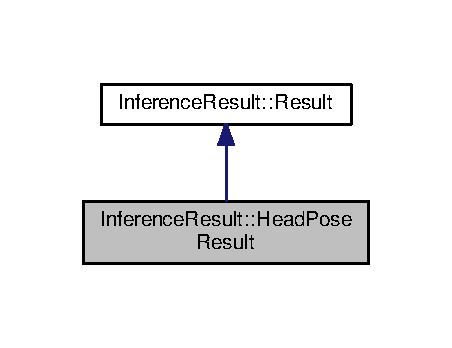
\includegraphics[width=217pt]{structInferenceResult_1_1HeadPoseResult__inherit__graph}
\end{center}
\end{figure}


Collaboration diagram for Inference\+Result\+:\+:Head\+Pose\+Result\+:
\nopagebreak
\begin{figure}[H]
\begin{center}
\leavevmode
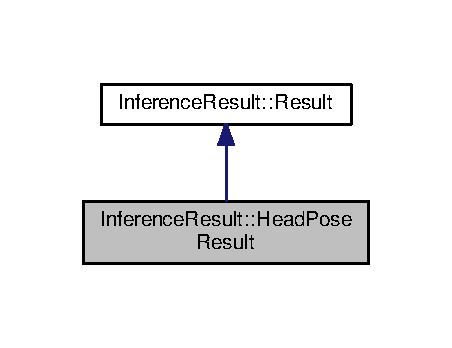
\includegraphics[width=217pt]{structInferenceResult_1_1HeadPoseResult__coll__graph}
\end{center}
\end{figure}
\subsection*{Public Attributes}
\begin{DoxyCompactItemize}
\item 
float \hyperlink{structInferenceResult_1_1HeadPoseResult_a6f9491752ad71d474f7b52f626bc6989}{angle\+\_\+y} = -\/1
\item 
float \hyperlink{structInferenceResult_1_1HeadPoseResult_aa5451224989c6d65741ff3a90e4c73a7}{angle\+\_\+p} = -\/1
\item 
float \hyperlink{structInferenceResult_1_1HeadPoseResult_a34e1aa51cf21ddc17d874260f174c75e}{angle\+\_\+r} = -\/1
\end{DoxyCompactItemize}


\subsection{Detailed Description}


Definition at line 29 of file data\+\_\+struct.\+h.



\subsection{Member Data Documentation}
\index{Inference\+Result\+::\+Head\+Pose\+Result@{Inference\+Result\+::\+Head\+Pose\+Result}!angle\+\_\+p@{angle\+\_\+p}}
\index{angle\+\_\+p@{angle\+\_\+p}!Inference\+Result\+::\+Head\+Pose\+Result@{Inference\+Result\+::\+Head\+Pose\+Result}}
\subsubsection[{\texorpdfstring{angle\+\_\+p}{angle_p}}]{\setlength{\rightskip}{0pt plus 5cm}float Inference\+Result\+::\+Head\+Pose\+Result\+::angle\+\_\+p = -\/1}\hypertarget{structInferenceResult_1_1HeadPoseResult_aa5451224989c6d65741ff3a90e4c73a7}{}\label{structInferenceResult_1_1HeadPoseResult_aa5451224989c6d65741ff3a90e4c73a7}


Definition at line 31 of file data\+\_\+struct.\+h.

\index{Inference\+Result\+::\+Head\+Pose\+Result@{Inference\+Result\+::\+Head\+Pose\+Result}!angle\+\_\+r@{angle\+\_\+r}}
\index{angle\+\_\+r@{angle\+\_\+r}!Inference\+Result\+::\+Head\+Pose\+Result@{Inference\+Result\+::\+Head\+Pose\+Result}}
\subsubsection[{\texorpdfstring{angle\+\_\+r}{angle_r}}]{\setlength{\rightskip}{0pt plus 5cm}float Inference\+Result\+::\+Head\+Pose\+Result\+::angle\+\_\+r = -\/1}\hypertarget{structInferenceResult_1_1HeadPoseResult_a34e1aa51cf21ddc17d874260f174c75e}{}\label{structInferenceResult_1_1HeadPoseResult_a34e1aa51cf21ddc17d874260f174c75e}


Definition at line 32 of file data\+\_\+struct.\+h.

\index{Inference\+Result\+::\+Head\+Pose\+Result@{Inference\+Result\+::\+Head\+Pose\+Result}!angle\+\_\+y@{angle\+\_\+y}}
\index{angle\+\_\+y@{angle\+\_\+y}!Inference\+Result\+::\+Head\+Pose\+Result@{Inference\+Result\+::\+Head\+Pose\+Result}}
\subsubsection[{\texorpdfstring{angle\+\_\+y}{angle_y}}]{\setlength{\rightskip}{0pt plus 5cm}float Inference\+Result\+::\+Head\+Pose\+Result\+::angle\+\_\+y = -\/1}\hypertarget{structInferenceResult_1_1HeadPoseResult_a6f9491752ad71d474f7b52f626bc6989}{}\label{structInferenceResult_1_1HeadPoseResult_a6f9491752ad71d474f7b52f626bc6989}


Definition at line 30 of file data\+\_\+struct.\+h.



The documentation for this struct was generated from the following file\+:\begin{DoxyCompactItemize}
\item 
include/openvino\+\_\+service/\hyperlink{data__struct_8h}{data\+\_\+struct.\+h}\end{DoxyCompactItemize}

\hypertarget{classImageDescription}{}\section{Image\+Description Class Reference}
\label{classImageDescription}\index{Image\+Description@{Image\+Description}}


{\ttfamily \#include $<$common.\+hpp$>$}

\subsection*{Public Member Functions}
\begin{DoxyCompactItemize}
\item 
\hyperlink{classImageDescription_a5306d6db34b16ff3ca9742e9036b025f}{Image\+Description} (const \hyperlink{CMakeLists_8txt_a548e427ae9357a6f3536cff3ca23efda}{std\+::list}$<$ \hyperlink{classDetectedObject}{Detected\+Object} $>$ \&\hyperlink{classImageDescription_aa814580e2dd58fc3442ddd3549e6d81d}{alist}, bool \hyperlink{classImageDescription_a4df135809acd954ad6882c2b805b2a5b}{check\+\_\+probs}=false)
\item 
\hyperlink{classImageDescription}{Image\+Description} \hyperlink{classImageDescription_a1b6675d07182ddf75a704b091daaa8ff}{scale} (float scale\+\_\+x, float scale\+\_\+y) const 
\end{DoxyCompactItemize}
\subsection*{Static Public Member Functions}
\begin{DoxyCompactItemize}
\item 
static float \hyperlink{classImageDescription_a2068c70b38a7c66811c7ca3acf1a6f80}{io\+U\+Multiple} (const \hyperlink{classImageDescription}{Image\+Description} \&detected\+Objects, const \hyperlink{classImageDescription}{Image\+Description} \&desired\+Objects)
\end{DoxyCompactItemize}
\subsection*{Public Attributes}
\begin{DoxyCompactItemize}
\item 
const \hyperlink{CMakeLists_8txt_a548e427ae9357a6f3536cff3ca23efda}{std\+::list}$<$ \hyperlink{classDetectedObject}{Detected\+Object} $>$ \hyperlink{classImageDescription_aa814580e2dd58fc3442ddd3549e6d81d}{alist}
\item 
const bool \hyperlink{classImageDescription_a4df135809acd954ad6882c2b805b2a5b}{check\+\_\+probs}
\end{DoxyCompactItemize}


\subsection{Detailed Description}


Definition at line 761 of file common.\+hpp.



\subsection{Constructor \& Destructor Documentation}
\index{Image\+Description@{Image\+Description}!Image\+Description@{Image\+Description}}
\index{Image\+Description@{Image\+Description}!Image\+Description@{Image\+Description}}
\subsubsection[{\texorpdfstring{Image\+Description(const std\+::list$<$ Detected\+Object $>$ \&alist, bool check\+\_\+probs=false)}{ImageDescription(const std::list< DetectedObject > &alist, bool check_probs=false)}}]{\setlength{\rightskip}{0pt plus 5cm}Image\+Description\+::\+Image\+Description (
\begin{DoxyParamCaption}
\item[{const {\bf std\+::list}$<$ {\bf Detected\+Object} $>$ \&}]{alist, }
\item[{bool}]{check\+\_\+probs = {\ttfamily false}}
\end{DoxyParamCaption}
)\hspace{0.3cm}{\ttfamily [inline]}, {\ttfamily [explicit]}}\hypertarget{classImageDescription_a5306d6db34b16ff3ca9742e9036b025f}{}\label{classImageDescription_a5306d6db34b16ff3ca9742e9036b025f}


Definition at line 766 of file common.\+hpp.


\begin{DoxyCode}
767             : \hyperlink{classImageDescription_aa814580e2dd58fc3442ddd3549e6d81d}{alist}(\hyperlink{classImageDescription_aa814580e2dd58fc3442ddd3549e6d81d}{alist}), \hyperlink{classImageDescription_a4df135809acd954ad6882c2b805b2a5b}{check\_probs}(\hyperlink{classImageDescription_a4df135809acd954ad6882c2b805b2a5b}{check\_probs}) \{
768     \}
\end{DoxyCode}


\subsection{Member Function Documentation}
\index{Image\+Description@{Image\+Description}!io\+U\+Multiple@{io\+U\+Multiple}}
\index{io\+U\+Multiple@{io\+U\+Multiple}!Image\+Description@{Image\+Description}}
\subsubsection[{\texorpdfstring{io\+U\+Multiple(const Image\+Description \&detected\+Objects, const Image\+Description \&desired\+Objects)}{ioUMultiple(const ImageDescription &detectedObjects, const ImageDescription &desiredObjects)}}]{\setlength{\rightskip}{0pt plus 5cm}static float Image\+Description\+::io\+U\+Multiple (
\begin{DoxyParamCaption}
\item[{const {\bf Image\+Description} \&}]{detected\+Objects, }
\item[{const {\bf Image\+Description} \&}]{desired\+Objects}
\end{DoxyParamCaption}
)\hspace{0.3cm}{\ttfamily [inline]}, {\ttfamily [static]}}\hypertarget{classImageDescription_a2068c70b38a7c66811c7ca3acf1a6f80}{}\label{classImageDescription_a2068c70b38a7c66811c7ca3acf1a6f80}


Definition at line 770 of file common.\+hpp.


\begin{DoxyCode}
770                                                                                                            
         \{
771         \textcolor{keyword}{const} \hyperlink{classImageDescription}{ImageDescription} *detectedObjectsSmall, *detectedObjectsBig;
772         \textcolor{keywordtype}{bool} \hyperlink{classImageDescription_a4df135809acd954ad6882c2b805b2a5b}{check\_probs} = desiredObjects.\hyperlink{classImageDescription_a4df135809acd954ad6882c2b805b2a5b}{check\_probs};
773 
774         \textcolor{keywordflow}{if} (detectedObjects.\hyperlink{classImageDescription_aa814580e2dd58fc3442ddd3549e6d81d}{alist}.size() < desiredObjects.\hyperlink{classImageDescription_aa814580e2dd58fc3442ddd3549e6d81d}{alist}.size()) \{
775             detectedObjectsSmall = &detectedObjects;
776             detectedObjectsBig = &desiredObjects;
777         \} \textcolor{keywordflow}{else} \{
778             detectedObjectsSmall = &desiredObjects;
779             detectedObjectsBig = &detectedObjects;
780         \}
781 
782         std::list<DetectedObject> doS = detectedObjectsSmall->\hyperlink{classImageDescription_aa814580e2dd58fc3442ddd3549e6d81d}{alist};
783         std::list<DetectedObject> doB = detectedObjectsBig->\hyperlink{classImageDescription_aa814580e2dd58fc3442ddd3549e6d81d}{alist};
784 
785         \textcolor{keywordtype}{float} fullScore = 0.0f;
786         \textcolor{keywordflow}{while} (doS.size() > 0) \{
787             \textcolor{keywordtype}{float} score = 0.0f;
788             std::list<DetectedObject>::iterator bestJ = doB.end();
789             \textcolor{keywordflow}{for} (\textcolor{keyword}{auto} j = doB.begin(); j != doB.end(); j++) \{
790                 \textcolor{keywordtype}{float} curscore = \hyperlink{classDetectedObject_abc68e001862990d52703deff97fe0db6}{DetectedObject::ioU}(*doS.begin(), *j);
791                 \textcolor{keywordflow}{if} (score < curscore) \{
792                     score = curscore;
793                     bestJ = j;
794                 \}
795             \}
796 
797             \textcolor{keywordtype}{float} coeff = 1.0;
798             \textcolor{keywordflow}{if} (check\_probs) \{
799                 \textcolor{keywordflow}{if} (bestJ != doB.end()) \{
800                     \hyperlink{classDetectedObject}{DetectedObject} test = *bestJ;
801                     \hyperlink{classDetectedObject}{DetectedObject} test1 = *doS.begin();
802                     \textcolor{keywordtype}{float} mn = std::min((*bestJ).prob, (*doS.begin()).prob);
803                     \textcolor{keywordtype}{float} mx = std::max((*bestJ).prob, (*doS.begin()).prob);
804 
805                     coeff = mn/mx;
806                 \}
807             \}
808 
809             doS.pop\_front();
810             \textcolor{keywordflow}{if} (bestJ != doB.end()) doB.erase(bestJ);
811             fullScore += coeff * score;
812         \}
813         fullScore /= detectedObjectsBig->\hyperlink{classImageDescription_aa814580e2dd58fc3442ddd3549e6d81d}{alist}.size();
814 
815 
816         \textcolor{keywordflow}{return} fullScore;
817     \}
\end{DoxyCode}
\index{Image\+Description@{Image\+Description}!scale@{scale}}
\index{scale@{scale}!Image\+Description@{Image\+Description}}
\subsubsection[{\texorpdfstring{scale(float scale\+\_\+x, float scale\+\_\+y) const }{scale(float scale_x, float scale_y) const }}]{\setlength{\rightskip}{0pt plus 5cm}{\bf Image\+Description} Image\+Description\+::scale (
\begin{DoxyParamCaption}
\item[{float}]{scale\+\_\+x, }
\item[{float}]{scale\+\_\+y}
\end{DoxyParamCaption}
) const\hspace{0.3cm}{\ttfamily [inline]}}\hypertarget{classImageDescription_a1b6675d07182ddf75a704b091daaa8ff}{}\label{classImageDescription_a1b6675d07182ddf75a704b091daaa8ff}


Definition at line 819 of file common.\+hpp.


\begin{DoxyCode}
819                                                                \{
820         std::list<DetectedObject> slist;
821         \textcolor{keywordflow}{for} (\textcolor{keyword}{auto}& dob : \hyperlink{classImageDescription_aa814580e2dd58fc3442ddd3549e6d81d}{alist}) \{
822             slist.push\_back(dob.scale(scale\_x, scale\_y));
823         \}
824         \textcolor{keywordflow}{return} \hyperlink{classImageDescription_a5306d6db34b16ff3ca9742e9036b025f}{ImageDescription}(slist, \hyperlink{classImageDescription_a4df135809acd954ad6882c2b805b2a5b}{check\_probs});
825     \}
\end{DoxyCode}


\subsection{Member Data Documentation}
\index{Image\+Description@{Image\+Description}!alist@{alist}}
\index{alist@{alist}!Image\+Description@{Image\+Description}}
\subsubsection[{\texorpdfstring{alist}{alist}}]{\setlength{\rightskip}{0pt plus 5cm}const {\bf std\+::list}$<${\bf Detected\+Object}$>$ Image\+Description\+::alist}\hypertarget{classImageDescription_aa814580e2dd58fc3442ddd3549e6d81d}{}\label{classImageDescription_aa814580e2dd58fc3442ddd3549e6d81d}


Definition at line 763 of file common.\+hpp.

\index{Image\+Description@{Image\+Description}!check\+\_\+probs@{check\+\_\+probs}}
\index{check\+\_\+probs@{check\+\_\+probs}!Image\+Description@{Image\+Description}}
\subsubsection[{\texorpdfstring{check\+\_\+probs}{check_probs}}]{\setlength{\rightskip}{0pt plus 5cm}const bool Image\+Description\+::check\+\_\+probs}\hypertarget{classImageDescription_a4df135809acd954ad6882c2b805b2a5b}{}\label{classImageDescription_a4df135809acd954ad6882c2b805b2a5b}


Definition at line 764 of file common.\+hpp.



The documentation for this class was generated from the following file\+:\begin{DoxyCompactItemize}
\item 
include/openvino\+\_\+service/\hyperlink{common_8hpp}{common.\+hpp}\end{DoxyCompactItemize}

\hypertarget{classImageWindow}{}\section{Image\+Window Class Reference}
\label{classImageWindow}\index{Image\+Window@{Image\+Window}}


{\ttfamily \#include $<$output.\+h$>$}



Inheritance diagram for Image\+Window\+:
\nopagebreak
\begin{figure}[H]
\begin{center}
\leavevmode
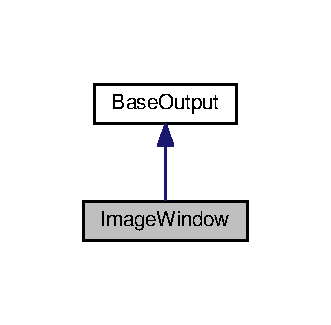
\includegraphics[width=159pt]{classImageWindow__inherit__graph}
\end{center}
\end{figure}


Collaboration diagram for Image\+Window\+:
\nopagebreak
\begin{figure}[H]
\begin{center}
\leavevmode
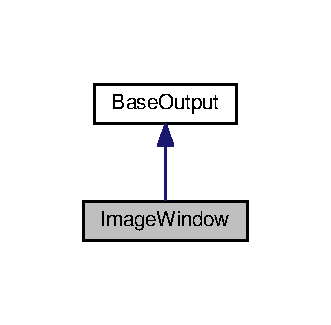
\includegraphics[width=159pt]{classImageWindow__coll__graph}
\end{center}
\end{figure}
\subsection*{Public Member Functions}
\begin{DoxyCompactItemize}
\item 
\hyperlink{classImageWindow_a5594e0624586cf492d52ee353348fa6d}{Image\+Window} (const std\+::string \&window\+\_\+name, \hyperlink{CMakeCache_8txt_a79a3d8790b2588b09777910863574e09}{int})
\item 
void \hyperlink{classImageWindow_a26fa3309cf79914dfe09b3b42b85e49e}{prepare\+Data} (const \hyperlink{structInferenceResult_1_1FaceDetectionResult}{Inference\+Result\+::\+Face\+Detection\+Result} \&) override
\item 
void \hyperlink{classImageWindow_a4fdaf7f1728e60672c22ddf57a4071b1}{prepare\+Data} (const \hyperlink{structInferenceResult_1_1EmotionsResult}{Inference\+Result\+::\+Emotions\+Result} \&) override
\item 
void \hyperlink{classImageWindow_a09a86f7b0c0e0eec807a4e1458a057c1}{prepare\+Data} (const \hyperlink{structInferenceResult_1_1AgeGenderResult}{Inference\+Result\+::\+Age\+Gender\+Result} \&) override
\item 
void \hyperlink{classImageWindow_abb0b9b0c103ec0460a2cbeee414b53c4}{prepare\+Data} (const \hyperlink{structInferenceResult_1_1HeadPoseResult}{Inference\+Result\+::\+Head\+Pose\+Result} \&) override
\item 
void \hyperlink{classImageWindow_a802e96acaba82b2f83eb3184c702fbcc}{feed\+Frame} (const cv\+::\+Mat \&) override
\item 
void \hyperlink{classImageWindow_a2927e0003c1f4579fb59aff50a9c7de3}{handle\+Output} (const std\+::string \&overall\+\_\+output\+\_\+text) override
\end{DoxyCompactItemize}


\subsection{Detailed Description}


Definition at line 30 of file output.\+h.



\subsection{Constructor \& Destructor Documentation}
\index{Image\+Window@{Image\+Window}!Image\+Window@{Image\+Window}}
\index{Image\+Window@{Image\+Window}!Image\+Window@{Image\+Window}}
\subsubsection[{\texorpdfstring{Image\+Window(const std\+::string \&window\+\_\+name, int)}{ImageWindow(const std::string &window_name, int)}}]{\setlength{\rightskip}{0pt plus 5cm}Image\+Window\+::\+Image\+Window (
\begin{DoxyParamCaption}
\item[{const std\+::string \&}]{window\+\_\+name, }
\item[{{\bf int}}]{focal\+\_\+length}
\end{DoxyParamCaption}
)\hspace{0.3cm}{\ttfamily [explicit]}}\hypertarget{classImageWindow_a5594e0624586cf492d52ee353348fa6d}{}\label{classImageWindow_a5594e0624586cf492d52ee353348fa6d}


Definition at line 7 of file output.\+cpp.


\begin{DoxyCode}
8                                                     :
9     window\_name\_(window\_name), focal\_length\_(focal\_length) \{
10   cv::namedWindow(window\_name, cv::WINDOW\_AUTOSIZE);
11 \}
\end{DoxyCode}


\subsection{Member Function Documentation}
\index{Image\+Window@{Image\+Window}!feed\+Frame@{feed\+Frame}}
\index{feed\+Frame@{feed\+Frame}!Image\+Window@{Image\+Window}}
\subsubsection[{\texorpdfstring{feed\+Frame(const cv\+::\+Mat \&) override}{feedFrame(const cv::Mat &) override}}]{\setlength{\rightskip}{0pt plus 5cm}void Image\+Window\+::feed\+Frame (
\begin{DoxyParamCaption}
\item[{const cv\+::\+Mat \&}]{frame}
\end{DoxyParamCaption}
)\hspace{0.3cm}{\ttfamily [override]}, {\ttfamily [virtual]}}\hypertarget{classImageWindow_a802e96acaba82b2f83eb3184c702fbcc}{}\label{classImageWindow_a802e96acaba82b2f83eb3184c702fbcc}


Reimplemented from \hyperlink{classBaseOutput_acdcbc58abecbf5671b1705937cd1cf02}{Base\+Output}.



Definition at line 13 of file output.\+cpp.


\begin{DoxyCode}
13                                               \{
14   frame\_ = frame;
15 \}
\end{DoxyCode}
\index{Image\+Window@{Image\+Window}!handle\+Output@{handle\+Output}}
\index{handle\+Output@{handle\+Output}!Image\+Window@{Image\+Window}}
\subsubsection[{\texorpdfstring{handle\+Output(const std\+::string \&overall\+\_\+output\+\_\+text) override}{handleOutput(const std::string &overall_output_text) override}}]{\setlength{\rightskip}{0pt plus 5cm}void Image\+Window\+::handle\+Output (
\begin{DoxyParamCaption}
\item[{const std\+::string \&}]{overall\+\_\+output\+\_\+text}
\end{DoxyParamCaption}
)\hspace{0.3cm}{\ttfamily [override]}, {\ttfamily [virtual]}}\hypertarget{classImageWindow_a2927e0003c1f4579fb59aff50a9c7de3}{}\label{classImageWindow_a2927e0003c1f4579fb59aff50a9c7de3}


Implements \hyperlink{classBaseOutput_ac516cfd7a05af7d710b5dd44d5b79878}{Base\+Output}.



Definition at line 166 of file output.\+cpp.


\begin{DoxyCode}
166                                                                    \{
167   cv::putText(frame\_,
168               overall\_output\_text,
169               cv::Point2f(0, 65),
170               cv::FONT\_HERSHEY\_TRIPLEX,
171               0.5,
172               cv::Scalar(255, 0, 0));
173   cv::imshow(window\_name\_, frame\_);
174 \}\end{DoxyCode}
\index{Image\+Window@{Image\+Window}!prepare\+Data@{prepare\+Data}}
\index{prepare\+Data@{prepare\+Data}!Image\+Window@{Image\+Window}}
\subsubsection[{\texorpdfstring{prepare\+Data(const Inference\+Result\+::\+Face\+Detection\+Result \&) override}{prepareData(const InferenceResult::FaceDetectionResult &) override}}]{\setlength{\rightskip}{0pt plus 5cm}void Image\+Window\+::prepare\+Data (
\begin{DoxyParamCaption}
\item[{const {\bf Inference\+Result\+::\+Face\+Detection\+Result} \&}]{result}
\end{DoxyParamCaption}
)\hspace{0.3cm}{\ttfamily [override]}, {\ttfamily [virtual]}}\hypertarget{classImageWindow_a26fa3309cf79914dfe09b3b42b85e49e}{}\label{classImageWindow_a26fa3309cf79914dfe09b3b42b85e49e}


Implements \hyperlink{classBaseOutput_ac8e9c0077758e64648fd1bd28661dec7}{Base\+Output}.



Definition at line 18 of file output.\+cpp.


\begin{DoxyCode}
18                                                                          \{
19   std::ostringstream out;
20   cv::Rect rect = result.\hyperlink{structInferenceResult_1_1Result_a20260cebf785b75132140ab517594660}{location};
21 
22   out.str(\textcolor{stringliteral}{""});
23   \textcolor{keywordflow}{if} (result.\hyperlink{structInferenceResult_1_1FaceDetectionResult_a7df2ce07767a0ef2c7b3ca27e9e20bc0}{confidence} >= 0) \{
24     out << \textcolor{stringliteral}{"face detection confidence: "}
25         << result.\hyperlink{structInferenceResult_1_1FaceDetectionResult_a395efa90912c78ac770588b57a474bd3}{label} << \textcolor{stringliteral}{": "}
26         << \hyperlink{CMakeCache_8txt_a4a461500e9bc62f37d07d326b178ef08}{std::fixed} << std::setprecision(3)
27         << result.\hyperlink{structInferenceResult_1_1FaceDetectionResult_a7df2ce07767a0ef2c7b3ca27e9e20bc0}{confidence} << \textcolor{stringliteral}{","};
28   \}
29   cv::putText(frame\_,
30               out.str(),
31               cv::Point2f(result.\hyperlink{structInferenceResult_1_1Result_a20260cebf785b75132140ab517594660}{location}.x, result.\hyperlink{structInferenceResult_1_1Result_a20260cebf785b75132140ab517594660}{location}.y - 15),
32               cv::FONT\_HERSHEY\_COMPLEX\_SMALL,
33               0.8,
34               cv::Scalar(0, 0, 255));
35   cv::rectangle(frame\_, result.\hyperlink{structInferenceResult_1_1Result_a20260cebf785b75132140ab517594660}{location}, cv::Scalar(100, 100, 100), 1);
36 \}
\end{DoxyCode}
\index{Image\+Window@{Image\+Window}!prepare\+Data@{prepare\+Data}}
\index{prepare\+Data@{prepare\+Data}!Image\+Window@{Image\+Window}}
\subsubsection[{\texorpdfstring{prepare\+Data(const Inference\+Result\+::\+Emotions\+Result \&) override}{prepareData(const InferenceResult::EmotionsResult &) override}}]{\setlength{\rightskip}{0pt plus 5cm}void Image\+Window\+::prepare\+Data (
\begin{DoxyParamCaption}
\item[{const {\bf Inference\+Result\+::\+Emotions\+Result} \&}]{result}
\end{DoxyParamCaption}
)\hspace{0.3cm}{\ttfamily [override]}, {\ttfamily [virtual]}}\hypertarget{classImageWindow_a4fdaf7f1728e60672c22ddf57a4071b1}{}\label{classImageWindow_a4fdaf7f1728e60672c22ddf57a4071b1}


Implements \hyperlink{classBaseOutput_a67d7a495441233da42b134667a312202}{Base\+Output}.



Definition at line 38 of file output.\+cpp.


\begin{DoxyCode}
38                                                                          \{
39   std::ostringstream out;
40   cv::Rect rect = result.\hyperlink{structInferenceResult_1_1Result_a20260cebf785b75132140ab517594660}{location};
41 
42   out.str(\textcolor{stringliteral}{""});
43   out << \textcolor{stringliteral}{"emotions detection confidence: "} <<
44       result.\hyperlink{structInferenceResult_1_1EmotionsResult_a273570a13673f51115a9de954cb0d333}{label} << \textcolor{stringliteral}{": "} <<
45       \hyperlink{CMakeCache_8txt_a4a461500e9bc62f37d07d326b178ef08}{std::fixed} << std::setprecision(3) <<
46       result.\hyperlink{structInferenceResult_1_1EmotionsResult_aec1805367ebc6acda383d180a3cc896e}{confidence} << \textcolor{stringliteral}{","};
47   cv::putText(frame\_,
48               out.str(),
49               cv::Point2f(result.\hyperlink{structInferenceResult_1_1Result_a20260cebf785b75132140ab517594660}{location}.x, result.\hyperlink{structInferenceResult_1_1Result_a20260cebf785b75132140ab517594660}{location}.y - 15),
50               cv::FONT\_HERSHEY\_COMPLEX\_SMALL,
51               0.8,
52               cv::Scalar(0, 0, 255));
53   cv::rectangle(frame\_, result.\hyperlink{structInferenceResult_1_1Result_a20260cebf785b75132140ab517594660}{location}, cv::Scalar(100, 100, 100), 1);
54 \}
\end{DoxyCode}
\index{Image\+Window@{Image\+Window}!prepare\+Data@{prepare\+Data}}
\index{prepare\+Data@{prepare\+Data}!Image\+Window@{Image\+Window}}
\subsubsection[{\texorpdfstring{prepare\+Data(const Inference\+Result\+::\+Age\+Gender\+Result \&) override}{prepareData(const InferenceResult::AgeGenderResult &) override}}]{\setlength{\rightskip}{0pt plus 5cm}void Image\+Window\+::prepare\+Data (
\begin{DoxyParamCaption}
\item[{const {\bf Inference\+Result\+::\+Age\+Gender\+Result} \&}]{result}
\end{DoxyParamCaption}
)\hspace{0.3cm}{\ttfamily [override]}, {\ttfamily [virtual]}}\hypertarget{classImageWindow_a09a86f7b0c0e0eec807a4e1458a057c1}{}\label{classImageWindow_a09a86f7b0c0e0eec807a4e1458a057c1}


Implements \hyperlink{classBaseOutput_a6a51c16ebfd7a58829bfa675e562b8f1}{Base\+Output}.



Definition at line 56 of file output.\+cpp.


\begin{DoxyCode}
56                                                                           \{
57   std::ostringstream out;
58   cv::Rect rect = result.\hyperlink{structInferenceResult_1_1Result_a20260cebf785b75132140ab517594660}{location};
59 
60   out.str(\textcolor{stringliteral}{""});
61   out << \textcolor{stringliteral}{"age gender detection confidence: "} <<
62       \textcolor{stringliteral}{"age is: "} << result.\hyperlink{structInferenceResult_1_1AgeGenderResult_a6c4ec413eb257cea2c02cc53a1cfc272}{age} << \textcolor{stringliteral}{","} <<
63       \textcolor{stringliteral}{"gender is: "} << (result.\hyperlink{structInferenceResult_1_1AgeGenderResult_a8a17d89e0d1b8bde9eb9d862486493c9}{male\_prob} > 0.5)? \textcolor{stringliteral}{"M"}:\textcolor{stringliteral}{"F"};
64   cv::putText(frame\_,
65               out.str(),
66               \textcolor{comment}{//cv::Point2f(result.location.x, result.location.y),}
67               cv::Point2f(0,30),
68               cv::FONT\_HERSHEY\_COMPLEX\_SMALL,
69               0.8,
70               cv::Scalar(0, 0, 255));
71   cv::rectangle(frame\_, result.\hyperlink{structInferenceResult_1_1Result_a20260cebf785b75132140ab517594660}{location}, cv::Scalar(100, 100, 100), 1);
72 \}
\end{DoxyCode}
\index{Image\+Window@{Image\+Window}!prepare\+Data@{prepare\+Data}}
\index{prepare\+Data@{prepare\+Data}!Image\+Window@{Image\+Window}}
\subsubsection[{\texorpdfstring{prepare\+Data(const Inference\+Result\+::\+Head\+Pose\+Result \&) override}{prepareData(const InferenceResult::HeadPoseResult &) override}}]{\setlength{\rightskip}{0pt plus 5cm}void Image\+Window\+::prepare\+Data (
\begin{DoxyParamCaption}
\item[{const {\bf Inference\+Result\+::\+Head\+Pose\+Result} \&}]{result}
\end{DoxyParamCaption}
)\hspace{0.3cm}{\ttfamily [override]}, {\ttfamily [virtual]}}\hypertarget{classImageWindow_abb0b9b0c103ec0460a2cbeee414b53c4}{}\label{classImageWindow_abb0b9b0c103ec0460a2cbeee414b53c4}


Implements \hyperlink{classBaseOutput_a3549ade1424963fff201fd946075fd4e}{Base\+Output}.



Definition at line 74 of file output.\+cpp.


\begin{DoxyCode}
74                                                                          \{
75   \textcolor{keywordtype}{int} scale  = 50;
76   \textcolor{keywordtype}{int} cx = frame\_.cols / 2;
77   \textcolor{keywordtype}{int} cy = frame\_.rows / 2;
78   \textcolor{keywordtype}{double} yaw = result.\hyperlink{structInferenceResult_1_1HeadPoseResult_a6f9491752ad71d474f7b52f626bc6989}{angle\_y} * CV\_PI / 180.0;
79   \textcolor{keywordtype}{double} pitch = result.\hyperlink{structInferenceResult_1_1HeadPoseResult_aa5451224989c6d65741ff3a90e4c73a7}{angle\_p} * CV\_PI / 180.0;
80   \textcolor{keywordtype}{double} roll = result.\hyperlink{structInferenceResult_1_1HeadPoseResult_a34e1aa51cf21ddc17d874260f174c75e}{angle\_r} * CV\_PI / 180.0;
81   cv::Rect rect = result.\hyperlink{structInferenceResult_1_1Result_a20260cebf785b75132140ab517594660}{location};
82   cv::Point3f cpoint(rect.x + rect.width / 2, rect.y + rect.height / 2, 0);
83   cv::Matx33f Rx(1, 0, 0,
84                  0, cos(pitch), -sin(pitch),
85                  0, sin(pitch), cos(pitch));
86   cv::Matx33f Ry(cos(yaw), 0, -sin(yaw),
87                  0, 1, 0,
88                  sin(yaw), 0, cos(yaw));
89   cv::Matx33f Rz(cos(roll), -sin(roll), 0,
90                  sin(roll), cos(roll), 0,
91                  0, 0, 1);
92 
93   \textcolor{keyword}{auto} r = cv::Mat(Rz * Ry * Rx);
94 
95   \textcolor{keywordflow}{if} (camera\_matrix\_.empty()) \{
96     camera\_matrix\_ = cv::Mat::zeros(3, 3, CV\_32F);
97     camera\_matrix\_.at<\textcolor{keywordtype}{float}>(0) = focal\_length\_;
98     camera\_matrix\_.at<\textcolor{keywordtype}{float}>(2) = static\_cast<float>(cx);
99     camera\_matrix\_.at<\textcolor{keywordtype}{float}>(4) = focal\_length\_;
100     camera\_matrix\_.at<\textcolor{keywordtype}{float}>(5) = static\_cast<float>(cy);
101     camera\_matrix\_.at<\textcolor{keywordtype}{float}>(8) = 1;
102   \}
103 
104   cv::Mat xAxis(3, 1, CV\_32F), yAxis(3, 1, CV\_32F), zAxis(3, 1, CV\_32F),
105       zAxis1(3, 1, CV\_32F);
106 
107   xAxis.at<\textcolor{keywordtype}{float}>(0) = 1 * scale;
108   xAxis.at<\textcolor{keywordtype}{float}>(1) = 0;
109   xAxis.at<\textcolor{keywordtype}{float}>(2) = 0;
110 
111   yAxis.at<\textcolor{keywordtype}{float}>(0) = 0;
112   yAxis.at<\textcolor{keywordtype}{float}>(1) = -1 * scale;
113   yAxis.at<\textcolor{keywordtype}{float}>(2) = 0;
114 
115   zAxis.at<\textcolor{keywordtype}{float}>(0) = 0;
116   zAxis.at<\textcolor{keywordtype}{float}>(1) = 0;
117   zAxis.at<\textcolor{keywordtype}{float}>(2) = -1 * scale;
118 
119   zAxis1.at<\textcolor{keywordtype}{float}>(0) = 0;
120   zAxis1.at<\textcolor{keywordtype}{float}>(1) = 0;
121   zAxis1.at<\textcolor{keywordtype}{float}>(2) = 1 * scale;
122 
123   cv::Mat o(3, 1, CV\_32F, cv::Scalar(0));
124   o.at<\textcolor{keywordtype}{float}>(2) = camera\_matrix\_.at<\textcolor{keywordtype}{float}>(0);
125 
126   xAxis = r * xAxis + o;
127   yAxis = r * yAxis + o;
128   zAxis = r * zAxis + o;
129   zAxis1 = r * zAxis1 + o;
130 
131   cv::Point p1, p2;
132 
133   p2.x = \textcolor{keyword}{static\_cast<}\textcolor{keywordtype}{int}\textcolor{keyword}{>}(
134       (xAxis.at<\textcolor{keywordtype}{float}>(0) / xAxis.at<\textcolor{keywordtype}{float}>(2) * camera\_matrix\_.at<\textcolor{keywordtype}{float}>(0))
135           + cpoint.x);
136   p2.y = \textcolor{keyword}{static\_cast<}\textcolor{keywordtype}{int}\textcolor{keyword}{>}(
137       (xAxis.at<\textcolor{keywordtype}{float}>(1) / xAxis.at<\textcolor{keywordtype}{float}>(2) * camera\_matrix\_.at<\textcolor{keywordtype}{float}>(4))
138           + cpoint.y);
139   cv::line(frame\_, cv::Point(cpoint.x, cpoint.y), p2, cv::Scalar(0, 0, 255), 2);
140 
141   p2.x = \textcolor{keyword}{static\_cast<}\textcolor{keywordtype}{int}\textcolor{keyword}{>}(
142       (yAxis.at<\textcolor{keywordtype}{float}>(0) / yAxis.at<\textcolor{keywordtype}{float}>(2) * camera\_matrix\_.at<\textcolor{keywordtype}{float}>(0))
143           + cpoint.x);
144   p2.y = \textcolor{keyword}{static\_cast<}\textcolor{keywordtype}{int}\textcolor{keyword}{>}(
145       (yAxis.at<\textcolor{keywordtype}{float}>(1) / yAxis.at<\textcolor{keywordtype}{float}>(2) * camera\_matrix\_.at<\textcolor{keywordtype}{float}>(4))
146           + cpoint.y);
147   cv::line(frame\_, cv::Point(cpoint.x, cpoint.y), p2, cv::Scalar(0, 255, 0), 2);
148 
149   p1.x = \textcolor{keyword}{static\_cast<}\textcolor{keywordtype}{int}\textcolor{keyword}{>}(
150       (zAxis1.at<\textcolor{keywordtype}{float}>(0) / zAxis1.at<\textcolor{keywordtype}{float}>(2) * camera\_matrix\_.at<\textcolor{keywordtype}{float}>(0))
151           + cpoint.x);
152   p1.y = \textcolor{keyword}{static\_cast<}\textcolor{keywordtype}{int}\textcolor{keyword}{>}(
153       (zAxis1.at<\textcolor{keywordtype}{float}>(1) / zAxis1.at<\textcolor{keywordtype}{float}>(2) * camera\_matrix\_.at<\textcolor{keywordtype}{float}>(4))
154           + cpoint.y);
155 
156   p2.x = \textcolor{keyword}{static\_cast<}\textcolor{keywordtype}{int}\textcolor{keyword}{>}(
157       (zAxis.at<\textcolor{keywordtype}{float}>(0) / zAxis.at<\textcolor{keywordtype}{float}>(2) * camera\_matrix\_.at<\textcolor{keywordtype}{float}>(0))
158           + cpoint.x);
159   p2.y = \textcolor{keyword}{static\_cast<}\textcolor{keywordtype}{int}\textcolor{keyword}{>}(
160       (zAxis.at<\textcolor{keywordtype}{float}>(1) / zAxis.at<\textcolor{keywordtype}{float}>(2) * camera\_matrix\_.at<\textcolor{keywordtype}{float}>(4))
161           + cpoint.y);
162   cv::line(frame\_, p1, p2, cv::Scalar(255, 0, 0), 2);
163   cv::circle(frame\_, p2, 3, cv::Scalar(255, 0, 0), 2);
164 \};
\end{DoxyCode}


The documentation for this class was generated from the following files\+:\begin{DoxyCompactItemize}
\item 
include/openvino\+\_\+service/outputs/\hyperlink{output_8h}{output.\+h}\item 
lib/outputs/\hyperlink{output_8cpp}{output.\+cpp}\end{DoxyCompactItemize}

\hypertarget{classInferenceEngine_1_1Extensions_1_1Cpu_1_1ImplFactory}{}\section{Inference\+Engine\+:\+:Extensions\+:\+:Cpu\+:\+:Impl\+Factory$<$ I\+M\+PL $>$ Class Template Reference}
\label{classInferenceEngine_1_1Extensions_1_1Cpu_1_1ImplFactory}\index{Inference\+Engine\+::\+Extensions\+::\+Cpu\+::\+Impl\+Factory$<$ I\+M\+P\+L $>$@{Inference\+Engine\+::\+Extensions\+::\+Cpu\+::\+Impl\+Factory$<$ I\+M\+P\+L $>$}}


{\ttfamily \#include $<$ext\+\_\+base.\+hpp$>$}



Inheritance diagram for Inference\+Engine\+:\+:Extensions\+:\+:Cpu\+:\+:Impl\+Factory$<$ I\+M\+PL $>$\+:
\nopagebreak
\begin{figure}[H]
\begin{center}
\leavevmode
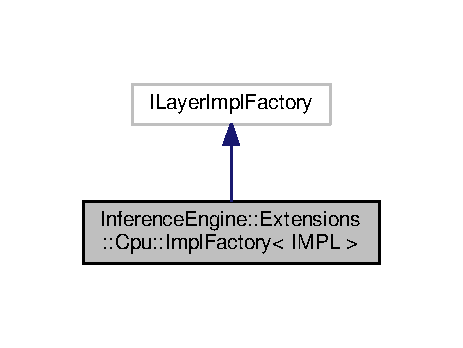
\includegraphics[width=222pt]{classInferenceEngine_1_1Extensions_1_1Cpu_1_1ImplFactory__inherit__graph}
\end{center}
\end{figure}


Collaboration diagram for Inference\+Engine\+:\+:Extensions\+:\+:Cpu\+:\+:Impl\+Factory$<$ I\+M\+PL $>$\+:
\nopagebreak
\begin{figure}[H]
\begin{center}
\leavevmode
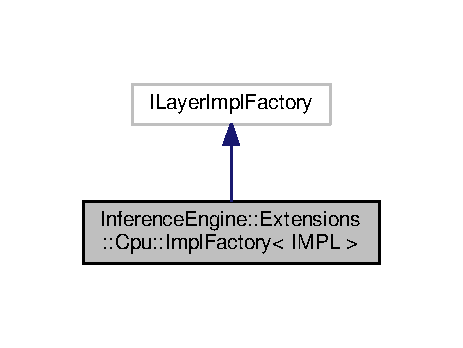
\includegraphics[width=222pt]{classInferenceEngine_1_1Extensions_1_1Cpu_1_1ImplFactory__coll__graph}
\end{center}
\end{figure}
\subsection*{Public Member Functions}
\begin{DoxyCompactItemize}
\item 
\hyperlink{classInferenceEngine_1_1Extensions_1_1Cpu_1_1ImplFactory_a86837f88ce5c196382c1f7c38e3ba3a8}{Impl\+Factory} (const C\+N\+N\+Layer $\ast$layer)
\item 
Status\+Code \hyperlink{classInferenceEngine_1_1Extensions_1_1Cpu_1_1ImplFactory_a93f5773c82ff0e8ec49496e86cdc1a68}{get\+Shapes} (const std\+::vector$<$ Tensor\+Desc $>$ \&in\+Shapes, std\+::vector$<$ Tensor\+Desc $>$ \&out\+Shapes, Response\+Desc $\ast$resp) noexceptoverride
\item 
Status\+Code \hyperlink{classInferenceEngine_1_1Extensions_1_1Cpu_1_1ImplFactory_a74b379a1a7dfae6fcc2c2b0146361802}{get\+Implementations} (std\+::vector$<$ I\+Layer\+Impl\+::\+Ptr $>$ \&impls, Response\+Desc $\ast$resp) noexceptoverride
\end{DoxyCompactItemize}
\subsection*{Protected Attributes}
\begin{DoxyCompactItemize}
\item 
C\+N\+N\+Layer \hyperlink{classInferenceEngine_1_1Extensions_1_1Cpu_1_1ImplFactory_a03cc9ae94115704d93b27a9a62b0619a}{cnn\+Layer}
\end{DoxyCompactItemize}


\subsection{Detailed Description}
\subsubsection*{template$<$class I\+M\+PL$>$\\*
class Inference\+Engine\+::\+Extensions\+::\+Cpu\+::\+Impl\+Factory$<$ I\+M\+P\+L $>$}



Definition at line 58 of file ext\+\_\+base.\+hpp.



\subsection{Constructor \& Destructor Documentation}
\index{Inference\+Engine\+::\+Extensions\+::\+Cpu\+::\+Impl\+Factory@{Inference\+Engine\+::\+Extensions\+::\+Cpu\+::\+Impl\+Factory}!Impl\+Factory@{Impl\+Factory}}
\index{Impl\+Factory@{Impl\+Factory}!Inference\+Engine\+::\+Extensions\+::\+Cpu\+::\+Impl\+Factory@{Inference\+Engine\+::\+Extensions\+::\+Cpu\+::\+Impl\+Factory}}
\subsubsection[{\texorpdfstring{Impl\+Factory(const C\+N\+N\+Layer $\ast$layer)}{ImplFactory(const CNNLayer *layer)}}]{\setlength{\rightskip}{0pt plus 5cm}template$<$class I\+M\+PL$>$ {\bf Inference\+Engine\+::\+Extensions\+::\+Cpu\+::\+Impl\+Factory}$<$ I\+M\+PL $>$\+::{\bf Impl\+Factory} (
\begin{DoxyParamCaption}
\item[{const C\+N\+N\+Layer $\ast$}]{layer}
\end{DoxyParamCaption}
)\hspace{0.3cm}{\ttfamily [inline]}, {\ttfamily [explicit]}}\hypertarget{classInferenceEngine_1_1Extensions_1_1Cpu_1_1ImplFactory_a86837f88ce5c196382c1f7c38e3ba3a8}{}\label{classInferenceEngine_1_1Extensions_1_1Cpu_1_1ImplFactory_a86837f88ce5c196382c1f7c38e3ba3a8}


Definition at line 60 of file ext\+\_\+base.\+hpp.


\begin{DoxyCode}
60 : \hyperlink{classInferenceEngine_1_1Extensions_1_1Cpu_1_1ImplFactory_a03cc9ae94115704d93b27a9a62b0619a}{cnnLayer}(*layer) \{\}
\end{DoxyCode}


\subsection{Member Function Documentation}
\index{Inference\+Engine\+::\+Extensions\+::\+Cpu\+::\+Impl\+Factory@{Inference\+Engine\+::\+Extensions\+::\+Cpu\+::\+Impl\+Factory}!get\+Implementations@{get\+Implementations}}
\index{get\+Implementations@{get\+Implementations}!Inference\+Engine\+::\+Extensions\+::\+Cpu\+::\+Impl\+Factory@{Inference\+Engine\+::\+Extensions\+::\+Cpu\+::\+Impl\+Factory}}
\subsubsection[{\texorpdfstring{get\+Implementations(std\+::vector$<$ I\+Layer\+Impl\+::\+Ptr $>$ \&impls, Response\+Desc $\ast$resp) noexceptoverride}{getImplementations(std::vector< ILayerImpl::Ptr > &impls, ResponseDesc *resp) noexceptoverride}}]{\setlength{\rightskip}{0pt plus 5cm}template$<$class I\+M\+PL$>$ Status\+Code {\bf Inference\+Engine\+::\+Extensions\+::\+Cpu\+::\+Impl\+Factory}$<$ I\+M\+PL $>$\+::get\+Implementations (
\begin{DoxyParamCaption}
\item[{std\+::vector$<$ I\+Layer\+Impl\+::\+Ptr $>$ \&}]{impls, }
\item[{Response\+Desc $\ast$}]{resp}
\end{DoxyParamCaption}
)\hspace{0.3cm}{\ttfamily [inline]}, {\ttfamily [override]}, {\ttfamily [noexcept]}}\hypertarget{classInferenceEngine_1_1Extensions_1_1Cpu_1_1ImplFactory_a74b379a1a7dfae6fcc2c2b0146361802}{}\label{classInferenceEngine_1_1Extensions_1_1Cpu_1_1ImplFactory_a74b379a1a7dfae6fcc2c2b0146361802}


Definition at line 68 of file ext\+\_\+base.\+hpp.


\begin{DoxyCode}
68                                                                                                          \{
69         impls.push\_back(ILayerImpl::Ptr(\textcolor{keyword}{new} IMPL(&\hyperlink{classInferenceEngine_1_1Extensions_1_1Cpu_1_1ImplFactory_a03cc9ae94115704d93b27a9a62b0619a}{cnnLayer})));
70         \textcolor{keywordflow}{return} OK;
71     \}
\end{DoxyCode}
\index{Inference\+Engine\+::\+Extensions\+::\+Cpu\+::\+Impl\+Factory@{Inference\+Engine\+::\+Extensions\+::\+Cpu\+::\+Impl\+Factory}!get\+Shapes@{get\+Shapes}}
\index{get\+Shapes@{get\+Shapes}!Inference\+Engine\+::\+Extensions\+::\+Cpu\+::\+Impl\+Factory@{Inference\+Engine\+::\+Extensions\+::\+Cpu\+::\+Impl\+Factory}}
\subsubsection[{\texorpdfstring{get\+Shapes(const std\+::vector$<$ Tensor\+Desc $>$ \&in\+Shapes, std\+::vector$<$ Tensor\+Desc $>$ \&out\+Shapes, Response\+Desc $\ast$resp) noexceptoverride}{getShapes(const std::vector< TensorDesc > &inShapes, std::vector< TensorDesc > &outShapes, ResponseDesc *resp) noexceptoverride}}]{\setlength{\rightskip}{0pt plus 5cm}template$<$class I\+M\+PL$>$ Status\+Code {\bf Inference\+Engine\+::\+Extensions\+::\+Cpu\+::\+Impl\+Factory}$<$ I\+M\+PL $>$\+::get\+Shapes (
\begin{DoxyParamCaption}
\item[{const std\+::vector$<$ Tensor\+Desc $>$ \&}]{in\+Shapes, }
\item[{std\+::vector$<$ Tensor\+Desc $>$ \&}]{out\+Shapes, }
\item[{Response\+Desc $\ast$}]{resp}
\end{DoxyParamCaption}
)\hspace{0.3cm}{\ttfamily [inline]}, {\ttfamily [override]}, {\ttfamily [noexcept]}}\hypertarget{classInferenceEngine_1_1Extensions_1_1Cpu_1_1ImplFactory_a93f5773c82ff0e8ec49496e86cdc1a68}{}\label{classInferenceEngine_1_1Extensions_1_1Cpu_1_1ImplFactory_a93f5773c82ff0e8ec49496e86cdc1a68}


Definition at line 62 of file ext\+\_\+base.\+hpp.


\begin{DoxyCode}
63                                                   \{
64         \textcolor{keywordflow}{return} NOT\_IMPLEMENTED;
65     \}
\end{DoxyCode}


\subsection{Member Data Documentation}
\index{Inference\+Engine\+::\+Extensions\+::\+Cpu\+::\+Impl\+Factory@{Inference\+Engine\+::\+Extensions\+::\+Cpu\+::\+Impl\+Factory}!cnn\+Layer@{cnn\+Layer}}
\index{cnn\+Layer@{cnn\+Layer}!Inference\+Engine\+::\+Extensions\+::\+Cpu\+::\+Impl\+Factory@{Inference\+Engine\+::\+Extensions\+::\+Cpu\+::\+Impl\+Factory}}
\subsubsection[{\texorpdfstring{cnn\+Layer}{cnnLayer}}]{\setlength{\rightskip}{0pt plus 5cm}template$<$class I\+M\+PL$>$ C\+N\+N\+Layer {\bf Inference\+Engine\+::\+Extensions\+::\+Cpu\+::\+Impl\+Factory}$<$ I\+M\+PL $>$\+::cnn\+Layer\hspace{0.3cm}{\ttfamily [protected]}}\hypertarget{classInferenceEngine_1_1Extensions_1_1Cpu_1_1ImplFactory_a03cc9ae94115704d93b27a9a62b0619a}{}\label{classInferenceEngine_1_1Extensions_1_1Cpu_1_1ImplFactory_a03cc9ae94115704d93b27a9a62b0619a}


Definition at line 74 of file ext\+\_\+base.\+hpp.



The documentation for this class was generated from the following file\+:\begin{DoxyCompactItemize}
\item 
thirdparty/extension/\hyperlink{ext__base_8hpp}{ext\+\_\+base.\+hpp}\end{DoxyCompactItemize}

\hypertarget{classInferenceEngine_1_1Extensions_1_1Cpu_1_1InterpImpl}{}\section{Inference\+Engine\+:\+:Extensions\+:\+:Cpu\+:\+:Interp\+Impl Class Reference}
\label{classInferenceEngine_1_1Extensions_1_1Cpu_1_1InterpImpl}\index{Inference\+Engine\+::\+Extensions\+::\+Cpu\+::\+Interp\+Impl@{Inference\+Engine\+::\+Extensions\+::\+Cpu\+::\+Interp\+Impl}}


Inheritance diagram for Inference\+Engine\+:\+:Extensions\+:\+:Cpu\+:\+:Interp\+Impl\+:
\nopagebreak
\begin{figure}[H]
\begin{center}
\leavevmode
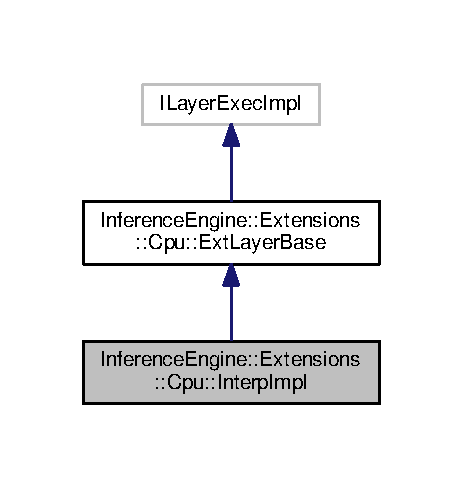
\includegraphics[width=222pt]{classInferenceEngine_1_1Extensions_1_1Cpu_1_1InterpImpl__inherit__graph}
\end{center}
\end{figure}


Collaboration diagram for Inference\+Engine\+:\+:Extensions\+:\+:Cpu\+:\+:Interp\+Impl\+:
\nopagebreak
\begin{figure}[H]
\begin{center}
\leavevmode
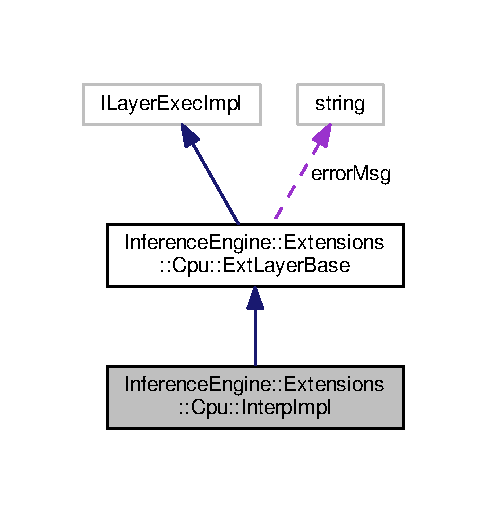
\includegraphics[width=234pt]{classInferenceEngine_1_1Extensions_1_1Cpu_1_1InterpImpl__coll__graph}
\end{center}
\end{figure}
\subsection*{Public Member Functions}
\begin{DoxyCompactItemize}
\item 
\hyperlink{classInferenceEngine_1_1Extensions_1_1Cpu_1_1InterpImpl_a0d0eba2fbd544ae96d2be310cefc2554}{Interp\+Impl} (const C\+N\+N\+Layer $\ast$layer)
\item 
Status\+Code \hyperlink{classInferenceEngine_1_1Extensions_1_1Cpu_1_1InterpImpl_a38d9a2dcf8e92268b177c25c5dcaa4f6}{execute} (std\+::vector$<$ Blob\+::\+Ptr $>$ \&inputs, std\+::vector$<$ Blob\+::\+Ptr $>$ \&outputs, Response\+Desc $\ast$resp) noexceptoverride
\end{DoxyCompactItemize}
\subsection*{Additional Inherited Members}


\subsection{Detailed Description}


Definition at line 26 of file ext\+\_\+interp.\+cpp.



\subsection{Constructor \& Destructor Documentation}
\index{Inference\+Engine\+::\+Extensions\+::\+Cpu\+::\+Interp\+Impl@{Inference\+Engine\+::\+Extensions\+::\+Cpu\+::\+Interp\+Impl}!Interp\+Impl@{Interp\+Impl}}
\index{Interp\+Impl@{Interp\+Impl}!Inference\+Engine\+::\+Extensions\+::\+Cpu\+::\+Interp\+Impl@{Inference\+Engine\+::\+Extensions\+::\+Cpu\+::\+Interp\+Impl}}
\subsubsection[{\texorpdfstring{Interp\+Impl(const C\+N\+N\+Layer $\ast$layer)}{InterpImpl(const CNNLayer *layer)}}]{\setlength{\rightskip}{0pt plus 5cm}Inference\+Engine\+::\+Extensions\+::\+Cpu\+::\+Interp\+Impl\+::\+Interp\+Impl (
\begin{DoxyParamCaption}
\item[{const C\+N\+N\+Layer $\ast$}]{layer}
\end{DoxyParamCaption}
)\hspace{0.3cm}{\ttfamily [inline]}, {\ttfamily [explicit]}}\hypertarget{classInferenceEngine_1_1Extensions_1_1Cpu_1_1InterpImpl_a0d0eba2fbd544ae96d2be310cefc2554}{}\label{classInferenceEngine_1_1Extensions_1_1Cpu_1_1InterpImpl_a0d0eba2fbd544ae96d2be310cefc2554}


Definition at line 28 of file ext\+\_\+interp.\+cpp.


\begin{DoxyCode}
28                                               : \hyperlink{classInferenceEngine_1_1Extensions_1_1Cpu_1_1ExtLayerBase_affff0e8263ca26852ccf71d299d7b06a}{ExtLayerBase}(layer) \{
29         \textcolor{keywordflow}{try} \{
30             \textcolor{keywordflow}{if} (\hyperlink{classInferenceEngine_1_1Extensions_1_1Cpu_1_1ExtLayerBase_a1074cdccacb9e9ca6eec01bbc2f7ca4a}{cnnLayer}.insData.size() != 1 || \hyperlink{classInferenceEngine_1_1Extensions_1_1Cpu_1_1ExtLayerBase_a1074cdccacb9e9ca6eec01bbc2f7ca4a}{cnnLayer}.outData.empty())
31                 THROW\_IE\_EXCEPTION << \textcolor{stringliteral}{"Incorrect number of input/output edges!"};
32 
33             \textcolor{keywordflow}{if} (\hyperlink{classInferenceEngine_1_1Extensions_1_1Cpu_1_1ExtLayerBase_a1074cdccacb9e9ca6eec01bbc2f7ca4a}{cnnLayer}.insData[0].lock()->dims.size() != 4)
34                 THROW\_IE\_EXCEPTION << \textcolor{stringliteral}{"Interp supports only 4d blobs!"};
35 
36             \textcolor{comment}{// We don't read other parameters since they are needed only for dst reshape in caffe}
37             pad\_beg = \hyperlink{classInferenceEngine_1_1Extensions_1_1Cpu_1_1ExtLayerBase_a1074cdccacb9e9ca6eec01bbc2f7ca4a}{cnnLayer}.GetParamAsInt(\textcolor{stringliteral}{"pad\_beg"});
38             pad\_end = \hyperlink{classInferenceEngine_1_1Extensions_1_1Cpu_1_1ExtLayerBase_a1074cdccacb9e9ca6eec01bbc2f7ca4a}{cnnLayer}.GetParamAsInt(\textcolor{stringliteral}{"pad\_end"});
39 
40 \textcolor{preprocessor}{#if defined(HAVE\_AVX512F)}
41             \textcolor{keyword}{auto} blk\_layout = \hyperlink{classInferenceEngine_1_1Extensions_1_1Cpu_1_1ExtLayerBase_a1258a8d209e0249e0b1717618352ddfba733623e98c6602d47f51e9f7be2f7d6c}{ConfLayout::BLK16};
42 \textcolor{preprocessor}{#else}
43             \textcolor{keyword}{auto} blk\_layout = \hyperlink{classInferenceEngine_1_1Extensions_1_1Cpu_1_1ExtLayerBase_a1258a8d209e0249e0b1717618352ddfba6023b7e0a175b8cf9cbcec3ac3cbf93d}{ConfLayout::BLK8};
44 \textcolor{preprocessor}{#endif}
45 
46             \hyperlink{classInferenceEngine_1_1Extensions_1_1Cpu_1_1ExtLayerBase_a0ac7a6632e95b9500d5246b05b4b0bfa}{addConfig}(\{DataConfigurator(blk\_layout)\}, \{DataConfigurator(blk\_layout)\});
47         \} \textcolor{keywordflow}{catch} (InferenceEngine::details::InferenceEngineException &ex) \{
48             \hyperlink{classInferenceEngine_1_1Extensions_1_1Cpu_1_1ExtLayerBase_abc78e9b5a79fa339ffd831a5318f71f7}{errorMsg} = ex.what();
49         \}
50     \}
\end{DoxyCode}


\subsection{Member Function Documentation}
\index{Inference\+Engine\+::\+Extensions\+::\+Cpu\+::\+Interp\+Impl@{Inference\+Engine\+::\+Extensions\+::\+Cpu\+::\+Interp\+Impl}!execute@{execute}}
\index{execute@{execute}!Inference\+Engine\+::\+Extensions\+::\+Cpu\+::\+Interp\+Impl@{Inference\+Engine\+::\+Extensions\+::\+Cpu\+::\+Interp\+Impl}}
\subsubsection[{\texorpdfstring{execute(std\+::vector$<$ Blob\+::\+Ptr $>$ \&inputs, std\+::vector$<$ Blob\+::\+Ptr $>$ \&outputs, Response\+Desc $\ast$resp) noexceptoverride}{execute(std::vector< Blob::Ptr > &inputs, std::vector< Blob::Ptr > &outputs, ResponseDesc *resp) noexceptoverride}}]{\setlength{\rightskip}{0pt plus 5cm}Status\+Code Inference\+Engine\+::\+Extensions\+::\+Cpu\+::\+Interp\+Impl\+::execute (
\begin{DoxyParamCaption}
\item[{std\+::vector$<$ Blob\+::\+Ptr $>$ \&}]{inputs, }
\item[{std\+::vector$<$ Blob\+::\+Ptr $>$ \&}]{outputs, }
\item[{Response\+Desc $\ast$}]{resp}
\end{DoxyParamCaption}
)\hspace{0.3cm}{\ttfamily [inline]}, {\ttfamily [override]}, {\ttfamily [noexcept]}}\hypertarget{classInferenceEngine_1_1Extensions_1_1Cpu_1_1InterpImpl_a38d9a2dcf8e92268b177c25c5dcaa4f6}{}\label{classInferenceEngine_1_1Extensions_1_1Cpu_1_1InterpImpl_a38d9a2dcf8e92268b177c25c5dcaa4f6}


Definition at line 52 of file ext\+\_\+interp.\+cpp.


\begin{DoxyCode}
53                                                              \{
54         \textcolor{keywordtype}{int} IN = \textcolor{keyword}{static\_cast<}\textcolor{keywordtype}{int}\textcolor{keyword}{>}(inputs[0]->getTensorDesc().getDims()[0]);
55         \textcolor{keywordtype}{int} IC = \textcolor{keyword}{static\_cast<}\textcolor{keywordtype}{int}\textcolor{keyword}{>}(inputs[0]->getTensorDesc().getDims()[1]);
56         \textcolor{keywordtype}{int} IH = \textcolor{keyword}{static\_cast<}\textcolor{keywordtype}{int}\textcolor{keyword}{>}(inputs[0]->getTensorDesc().getDims()[2]);
57         \textcolor{keywordtype}{int} IW = \textcolor{keyword}{static\_cast<}\textcolor{keywordtype}{int}\textcolor{keyword}{>}(inputs[0]->getTensorDesc().getDims()[3]);
58 
59         \textcolor{keywordtype}{int} OH = \textcolor{keyword}{static\_cast<}\textcolor{keywordtype}{int}\textcolor{keyword}{>}(outputs[0]->getTensorDesc().getDims()[2]);
60         \textcolor{keywordtype}{int} OW = \textcolor{keyword}{static\_cast<}\textcolor{keywordtype}{int}\textcolor{keyword}{>}(outputs[0]->getTensorDesc().getDims()[3]);
61 
62         \textcolor{keywordtype}{int} IH\_pad = IH + pad\_beg + pad\_end;
63         \textcolor{keywordtype}{int} IW\_pad = IW + pad\_beg + pad\_end;
64 
65         \textcolor{keyword}{const} \textcolor{keyword}{auto} *src\_data = inputs[0]->buffer().as<\textcolor{keyword}{const} \textcolor{keywordtype}{float} *>();
66         \textcolor{keyword}{auto} *dst\_data = outputs[0]->buffer().as<\textcolor{keywordtype}{float} *>();
67 
68         interpolate(IN, IC, src\_data, -pad\_beg, -pad\_beg, IH\_pad, IW\_pad, IH, IW, dst\_data, 0, 0, OH, OW, 
      OH, OW);
69         \textcolor{keywordflow}{return} OK;
70     \}
\end{DoxyCode}


The documentation for this class was generated from the following file\+:\begin{DoxyCompactItemize}
\item 
thirdparty/extension/\hyperlink{ext__interp_8cpp}{ext\+\_\+interp.\+cpp}\end{DoxyCompactItemize}

\hypertarget{classslog_1_1LogStream}{}\section{slog\+:\+:Log\+Stream Class Reference}
\label{classslog_1_1LogStream}\index{slog\+::\+Log\+Stream@{slog\+::\+Log\+Stream}}


The \hyperlink{classslog_1_1LogStream}{Log\+Stream} class implements a stream for sample logging.  




{\ttfamily \#include $<$slog.\+hpp$>$}

\subsection*{Public Member Functions}
\begin{DoxyCompactItemize}
\item 
\hyperlink{classslog_1_1LogStream_ae6947cb3d25a84ca7853b5e62579c257}{Log\+Stream} (const std\+::string \&prefix, std\+::ostream \&log\+\_\+stream)
\begin{DoxyCompactList}\small\item\em A constructor. Creates an \hyperlink{classslog_1_1LogStream}{Log\+Stream} object. \end{DoxyCompactList}\item 
{\footnotesize template$<$class T $>$ }\\\hyperlink{classslog_1_1LogStream}{Log\+Stream} \& \hyperlink{classslog_1_1LogStream_ac265c41ce68be9f1b42e540e99e4f182}{operator$<$$<$} (const T \&arg)
\begin{DoxyCompactList}\small\item\em A stream output operator to be used within the logger. \end{DoxyCompactList}\item 
\hyperlink{classslog_1_1LogStream}{Log\+Stream} \& \hyperlink{classslog_1_1LogStream_adbbee3626b1771055c484a67272e905b}{operator$<$$<$} (const \hyperlink{classslog_1_1LogStreamEndLine}{Log\+Stream\+End\+Line} \&arg)
\end{DoxyCompactItemize}


\subsection{Detailed Description}
The \hyperlink{classslog_1_1LogStream}{Log\+Stream} class implements a stream for sample logging. 

Definition at line 42 of file slog.\+hpp.



\subsection{Constructor \& Destructor Documentation}
\index{slog\+::\+Log\+Stream@{slog\+::\+Log\+Stream}!Log\+Stream@{Log\+Stream}}
\index{Log\+Stream@{Log\+Stream}!slog\+::\+Log\+Stream@{slog\+::\+Log\+Stream}}
\subsubsection[{\texorpdfstring{Log\+Stream(const std\+::string \&prefix, std\+::ostream \&log\+\_\+stream)}{LogStream(const std::string &prefix, std::ostream &log_stream)}}]{\setlength{\rightskip}{0pt plus 5cm}slog\+::\+Log\+Stream\+::\+Log\+Stream (
\begin{DoxyParamCaption}
\item[{const std\+::string \&}]{prefix, }
\item[{std\+::ostream \&}]{log\+\_\+stream}
\end{DoxyParamCaption}
)\hspace{0.3cm}{\ttfamily [inline]}}\hypertarget{classslog_1_1LogStream_ae6947cb3d25a84ca7853b5e62579c257}{}\label{classslog_1_1LogStream_ae6947cb3d25a84ca7853b5e62579c257}


A constructor. Creates an \hyperlink{classslog_1_1LogStream}{Log\+Stream} object. 


\begin{DoxyParams}{Parameters}
{\em prefix} & The prefix to print \\
\hline
\end{DoxyParams}


Definition at line 52 of file slog.\+hpp.


\begin{DoxyCode}
53             : \_prefix(prefix), \_new\_line(\textcolor{keyword}{true}) \{
54         \_log\_stream = &log\_stream;
55     \}
\end{DoxyCode}


\subsection{Member Function Documentation}
\index{slog\+::\+Log\+Stream@{slog\+::\+Log\+Stream}!operator$<$$<$@{operator$<$$<$}}
\index{operator$<$$<$@{operator$<$$<$}!slog\+::\+Log\+Stream@{slog\+::\+Log\+Stream}}
\subsubsection[{\texorpdfstring{operator$<$$<$(const T \&arg)}{operator<<(const T &arg)}}]{\setlength{\rightskip}{0pt plus 5cm}template$<$class T $>$ {\bf Log\+Stream}\& slog\+::\+Log\+Stream\+::operator$<$$<$ (
\begin{DoxyParamCaption}
\item[{const T \&}]{arg}
\end{DoxyParamCaption}
)\hspace{0.3cm}{\ttfamily [inline]}}\hypertarget{classslog_1_1LogStream_ac265c41ce68be9f1b42e540e99e4f182}{}\label{classslog_1_1LogStream_ac265c41ce68be9f1b42e540e99e4f182}


A stream output operator to be used within the logger. 


\begin{DoxyParams}{Parameters}
{\em arg} & Object for serialization in the logger message \\
\hline
\end{DoxyParams}


Definition at line 62 of file slog.\+hpp.


\begin{DoxyCode}
62                                         \{
63         \textcolor{keywordflow}{if} (\_new\_line) \{
64             (*\_log\_stream) << \textcolor{stringliteral}{"[ "} << \_prefix << \textcolor{stringliteral}{" ] "};
65             \_new\_line = \textcolor{keyword}{false};
66         \}
67 
68         (*\_log\_stream) << arg;
69         \textcolor{keywordflow}{return} *\textcolor{keyword}{this};
70     \}
\end{DoxyCode}
\index{slog\+::\+Log\+Stream@{slog\+::\+Log\+Stream}!operator$<$$<$@{operator$<$$<$}}
\index{operator$<$$<$@{operator$<$$<$}!slog\+::\+Log\+Stream@{slog\+::\+Log\+Stream}}
\subsubsection[{\texorpdfstring{operator$<$$<$(const Log\+Stream\+End\+Line \&arg)}{operator<<(const LogStreamEndLine &arg)}}]{\setlength{\rightskip}{0pt plus 5cm}{\bf Log\+Stream}\& slog\+::\+Log\+Stream\+::operator$<$$<$ (
\begin{DoxyParamCaption}
\item[{const {\bf Log\+Stream\+End\+Line} \&}]{arg}
\end{DoxyParamCaption}
)\hspace{0.3cm}{\ttfamily [inline]}}\hypertarget{classslog_1_1LogStream_adbbee3626b1771055c484a67272e905b}{}\label{classslog_1_1LogStream_adbbee3626b1771055c484a67272e905b}


Definition at line 73 of file slog.\+hpp.


\begin{DoxyCode}
73                                                         \{
74         \_new\_line = \textcolor{keyword}{true};
75 
76         (*\_log\_stream) << std::endl;
77         \textcolor{keywordflow}{return} *\textcolor{keyword}{this};
78     \}
\end{DoxyCode}


The documentation for this class was generated from the following file\+:\begin{DoxyCompactItemize}
\item 
include/openvino\+\_\+service/\hyperlink{slog_8hpp}{slog.\+hpp}\end{DoxyCompactItemize}

\hypertarget{classslog_1_1LogStreamEndLine}{}\section{slog\+:\+:Log\+Stream\+End\+Line Class Reference}
\label{classslog_1_1LogStreamEndLine}\index{slog\+::\+Log\+Stream\+End\+Line@{slog\+::\+Log\+Stream\+End\+Line}}


The \hyperlink{classslog_1_1LogStreamEndLine}{Log\+Stream\+End\+Line} class implements an end line marker for a log stream.  




{\ttfamily \#include $<$slog.\+hpp$>$}



\subsection{Detailed Description}
The \hyperlink{classslog_1_1LogStreamEndLine}{Log\+Stream\+End\+Line} class implements an end line marker for a log stream. 

Definition at line 33 of file slog.\+hpp.



The documentation for this class was generated from the following file\+:\begin{DoxyCompactItemize}
\item 
include/openvino\+\_\+service/\hyperlink{slog_8hpp}{slog.\+hpp}\end{DoxyCompactItemize}

\hypertarget{classMUTEX__NAMESPACE_1_1Mutex}{}\section{M\+U\+T\+E\+X\+\_\+\+N\+A\+M\+E\+S\+P\+A\+CE\+:\+:Mutex Class Reference}
\label{classMUTEX__NAMESPACE_1_1Mutex}\index{M\+U\+T\+E\+X\+\_\+\+N\+A\+M\+E\+S\+P\+A\+C\+E\+::\+Mutex@{M\+U\+T\+E\+X\+\_\+\+N\+A\+M\+E\+S\+P\+A\+C\+E\+::\+Mutex}}


{\ttfamily \#include $<$mutex.\+h$>$}

\subsection*{Public Types}
\begin{DoxyCompactItemize}
\item 
enum \hyperlink{classMUTEX__NAMESPACE_1_1Mutex_adc86cefc61118aec82af3bc8bb90e0c0}{Linker\+Initialized} \{ \hyperlink{classMUTEX__NAMESPACE_1_1Mutex_adc86cefc61118aec82af3bc8bb90e0c0a1e3df83eb608cf9744b540a9f395c9ea}{L\+I\+N\+K\+E\+R\+\_\+\+I\+N\+I\+T\+I\+A\+L\+I\+Z\+ED}
 \}
\end{DoxyCompactItemize}
\subsection*{Public Member Functions}
\begin{DoxyCompactItemize}
\item 
\hyperlink{classMUTEX__NAMESPACE_1_1Mutex_a87bdc59b403697dca13cc4d7e6974897}{Mutex} ()
\item 
\hyperlink{classMUTEX__NAMESPACE_1_1Mutex_a28876311c986326e09705075fe425681}{Mutex} (\hyperlink{classMUTEX__NAMESPACE_1_1Mutex_adc86cefc61118aec82af3bc8bb90e0c0}{Linker\+Initialized})
\item 
\hyperlink{classMUTEX__NAMESPACE_1_1Mutex_a70c8725a5b4241215ea90174990deda0}{$\sim$\+Mutex} ()
\item 
void \hyperlink{classMUTEX__NAMESPACE_1_1Mutex_a0bf14b5dcd3d7f5f5b526c18792b1737}{Lock} ()
\item 
void \hyperlink{classMUTEX__NAMESPACE_1_1Mutex_a10c6e61df4a205e3693429b4d285fbab}{Unlock} ()
\item 
void \hyperlink{classMUTEX__NAMESPACE_1_1Mutex_a90b6daa95b7f0457d5f2b6003d31d48a}{Reader\+Lock} ()
\item 
void \hyperlink{classMUTEX__NAMESPACE_1_1Mutex_a793db8b25b595af5a81084b09b08955d}{Reader\+Unlock} ()
\item 
void \hyperlink{classMUTEX__NAMESPACE_1_1Mutex_ab6100d175d29d05343e252caa2e48e39}{Writer\+Lock} ()
\item 
void \hyperlink{classMUTEX__NAMESPACE_1_1Mutex_a4cb60398bf6ab0ffdab9bcd27c5c705c}{Writer\+Unlock} ()
\end{DoxyCompactItemize}


\subsection{Detailed Description}


Definition at line 157 of file mutex.\+h.



\subsection{Member Enumeration Documentation}
\index{M\+U\+T\+E\+X\+\_\+\+N\+A\+M\+E\+S\+P\+A\+C\+E\+::\+Mutex@{M\+U\+T\+E\+X\+\_\+\+N\+A\+M\+E\+S\+P\+A\+C\+E\+::\+Mutex}!Linker\+Initialized@{Linker\+Initialized}}
\index{Linker\+Initialized@{Linker\+Initialized}!M\+U\+T\+E\+X\+\_\+\+N\+A\+M\+E\+S\+P\+A\+C\+E\+::\+Mutex@{M\+U\+T\+E\+X\+\_\+\+N\+A\+M\+E\+S\+P\+A\+C\+E\+::\+Mutex}}
\subsubsection[{\texorpdfstring{Linker\+Initialized}{LinkerInitialized}}]{\setlength{\rightskip}{0pt plus 5cm}enum {\bf M\+U\+T\+E\+X\+\_\+\+N\+A\+M\+E\+S\+P\+A\+C\+E\+::\+Mutex\+::\+Linker\+Initialized}}\hypertarget{classMUTEX__NAMESPACE_1_1Mutex_adc86cefc61118aec82af3bc8bb90e0c0}{}\label{classMUTEX__NAMESPACE_1_1Mutex_adc86cefc61118aec82af3bc8bb90e0c0}
\begin{Desc}
\item[Enumerator]\par
\begin{description}
\index{L\+I\+N\+K\+E\+R\+\_\+\+I\+N\+I\+T\+I\+A\+L\+I\+Z\+ED@{L\+I\+N\+K\+E\+R\+\_\+\+I\+N\+I\+T\+I\+A\+L\+I\+Z\+ED}!M\+U\+T\+E\+X\+\_\+\+N\+A\+M\+E\+S\+P\+A\+C\+E\+::\+Mutex@{M\+U\+T\+E\+X\+\_\+\+N\+A\+M\+E\+S\+P\+A\+C\+E\+::\+Mutex}}\index{M\+U\+T\+E\+X\+\_\+\+N\+A\+M\+E\+S\+P\+A\+C\+E\+::\+Mutex@{M\+U\+T\+E\+X\+\_\+\+N\+A\+M\+E\+S\+P\+A\+C\+E\+::\+Mutex}!L\+I\+N\+K\+E\+R\+\_\+\+I\+N\+I\+T\+I\+A\+L\+I\+Z\+ED@{L\+I\+N\+K\+E\+R\+\_\+\+I\+N\+I\+T\+I\+A\+L\+I\+Z\+ED}}\item[{\em 
L\+I\+N\+K\+E\+R\+\_\+\+I\+N\+I\+T\+I\+A\+L\+I\+Z\+ED\hypertarget{classMUTEX__NAMESPACE_1_1Mutex_adc86cefc61118aec82af3bc8bb90e0c0a1e3df83eb608cf9744b540a9f395c9ea}{}\label{classMUTEX__NAMESPACE_1_1Mutex_adc86cefc61118aec82af3bc8bb90e0c0a1e3df83eb608cf9744b540a9f395c9ea}
}]\end{description}
\end{Desc}


Definition at line 160 of file mutex.\+h.


\begin{DoxyCode}
160 \{ \hyperlink{classMUTEX__NAMESPACE_1_1Mutex_adc86cefc61118aec82af3bc8bb90e0c0a1e3df83eb608cf9744b540a9f395c9ea}{LINKER\_INITIALIZED} \};
\end{DoxyCode}


\subsection{Constructor \& Destructor Documentation}
\index{M\+U\+T\+E\+X\+\_\+\+N\+A\+M\+E\+S\+P\+A\+C\+E\+::\+Mutex@{M\+U\+T\+E\+X\+\_\+\+N\+A\+M\+E\+S\+P\+A\+C\+E\+::\+Mutex}!Mutex@{Mutex}}
\index{Mutex@{Mutex}!M\+U\+T\+E\+X\+\_\+\+N\+A\+M\+E\+S\+P\+A\+C\+E\+::\+Mutex@{M\+U\+T\+E\+X\+\_\+\+N\+A\+M\+E\+S\+P\+A\+C\+E\+::\+Mutex}}
\subsubsection[{\texorpdfstring{Mutex()}{Mutex()}}]{\setlength{\rightskip}{0pt plus 5cm}M\+U\+T\+E\+X\+\_\+\+N\+A\+M\+E\+S\+P\+A\+C\+E\+::\+Mutex\+::\+Mutex (
\begin{DoxyParamCaption}
{}
\end{DoxyParamCaption}
)\hspace{0.3cm}{\ttfamily [inline]}}\hypertarget{classMUTEX__NAMESPACE_1_1Mutex_a87bdc59b403697dca13cc4d7e6974897}{}\label{classMUTEX__NAMESPACE_1_1Mutex_a87bdc59b403697dca13cc4d7e6974897}
\index{M\+U\+T\+E\+X\+\_\+\+N\+A\+M\+E\+S\+P\+A\+C\+E\+::\+Mutex@{M\+U\+T\+E\+X\+\_\+\+N\+A\+M\+E\+S\+P\+A\+C\+E\+::\+Mutex}!Mutex@{Mutex}}
\index{Mutex@{Mutex}!M\+U\+T\+E\+X\+\_\+\+N\+A\+M\+E\+S\+P\+A\+C\+E\+::\+Mutex@{M\+U\+T\+E\+X\+\_\+\+N\+A\+M\+E\+S\+P\+A\+C\+E\+::\+Mutex}}
\subsubsection[{\texorpdfstring{Mutex(\+Linker\+Initialized)}{Mutex(LinkerInitialized)}}]{\setlength{\rightskip}{0pt plus 5cm}M\+U\+T\+E\+X\+\_\+\+N\+A\+M\+E\+S\+P\+A\+C\+E\+::\+Mutex\+::\+Mutex (
\begin{DoxyParamCaption}
\item[{{\bf Linker\+Initialized}}]{}
\end{DoxyParamCaption}
)\hspace{0.3cm}{\ttfamily [inline]}, {\ttfamily [explicit]}}\hypertarget{classMUTEX__NAMESPACE_1_1Mutex_a28876311c986326e09705075fe425681}{}\label{classMUTEX__NAMESPACE_1_1Mutex_a28876311c986326e09705075fe425681}
\index{M\+U\+T\+E\+X\+\_\+\+N\+A\+M\+E\+S\+P\+A\+C\+E\+::\+Mutex@{M\+U\+T\+E\+X\+\_\+\+N\+A\+M\+E\+S\+P\+A\+C\+E\+::\+Mutex}!````~Mutex@{$\sim$\+Mutex}}
\index{````~Mutex@{$\sim$\+Mutex}!M\+U\+T\+E\+X\+\_\+\+N\+A\+M\+E\+S\+P\+A\+C\+E\+::\+Mutex@{M\+U\+T\+E\+X\+\_\+\+N\+A\+M\+E\+S\+P\+A\+C\+E\+::\+Mutex}}
\subsubsection[{\texorpdfstring{$\sim$\+Mutex()}{~Mutex()}}]{\setlength{\rightskip}{0pt plus 5cm}M\+U\+T\+E\+X\+\_\+\+N\+A\+M\+E\+S\+P\+A\+C\+E\+::\+Mutex\+::$\sim$\+Mutex (
\begin{DoxyParamCaption}
{}
\end{DoxyParamCaption}
)\hspace{0.3cm}{\ttfamily [inline]}}\hypertarget{classMUTEX__NAMESPACE_1_1Mutex_a70c8725a5b4241215ea90174990deda0}{}\label{classMUTEX__NAMESPACE_1_1Mutex_a70c8725a5b4241215ea90174990deda0}


\subsection{Member Function Documentation}
\index{M\+U\+T\+E\+X\+\_\+\+N\+A\+M\+E\+S\+P\+A\+C\+E\+::\+Mutex@{M\+U\+T\+E\+X\+\_\+\+N\+A\+M\+E\+S\+P\+A\+C\+E\+::\+Mutex}!Lock@{Lock}}
\index{Lock@{Lock}!M\+U\+T\+E\+X\+\_\+\+N\+A\+M\+E\+S\+P\+A\+C\+E\+::\+Mutex@{M\+U\+T\+E\+X\+\_\+\+N\+A\+M\+E\+S\+P\+A\+C\+E\+::\+Mutex}}
\subsubsection[{\texorpdfstring{Lock()}{Lock()}}]{\setlength{\rightskip}{0pt plus 5cm}void M\+U\+T\+E\+X\+\_\+\+N\+A\+M\+E\+S\+P\+A\+C\+E\+::\+Mutex\+::\+Lock (
\begin{DoxyParamCaption}
{}
\end{DoxyParamCaption}
)\hspace{0.3cm}{\ttfamily [inline]}}\hypertarget{classMUTEX__NAMESPACE_1_1Mutex_a0bf14b5dcd3d7f5f5b526c18792b1737}{}\label{classMUTEX__NAMESPACE_1_1Mutex_a0bf14b5dcd3d7f5f5b526c18792b1737}
\index{M\+U\+T\+E\+X\+\_\+\+N\+A\+M\+E\+S\+P\+A\+C\+E\+::\+Mutex@{M\+U\+T\+E\+X\+\_\+\+N\+A\+M\+E\+S\+P\+A\+C\+E\+::\+Mutex}!Reader\+Lock@{Reader\+Lock}}
\index{Reader\+Lock@{Reader\+Lock}!M\+U\+T\+E\+X\+\_\+\+N\+A\+M\+E\+S\+P\+A\+C\+E\+::\+Mutex@{M\+U\+T\+E\+X\+\_\+\+N\+A\+M\+E\+S\+P\+A\+C\+E\+::\+Mutex}}
\subsubsection[{\texorpdfstring{Reader\+Lock()}{ReaderLock()}}]{\setlength{\rightskip}{0pt plus 5cm}void M\+U\+T\+E\+X\+\_\+\+N\+A\+M\+E\+S\+P\+A\+C\+E\+::\+Mutex\+::\+Reader\+Lock (
\begin{DoxyParamCaption}
{}
\end{DoxyParamCaption}
)\hspace{0.3cm}{\ttfamily [inline]}}\hypertarget{classMUTEX__NAMESPACE_1_1Mutex_a90b6daa95b7f0457d5f2b6003d31d48a}{}\label{classMUTEX__NAMESPACE_1_1Mutex_a90b6daa95b7f0457d5f2b6003d31d48a}
\index{M\+U\+T\+E\+X\+\_\+\+N\+A\+M\+E\+S\+P\+A\+C\+E\+::\+Mutex@{M\+U\+T\+E\+X\+\_\+\+N\+A\+M\+E\+S\+P\+A\+C\+E\+::\+Mutex}!Reader\+Unlock@{Reader\+Unlock}}
\index{Reader\+Unlock@{Reader\+Unlock}!M\+U\+T\+E\+X\+\_\+\+N\+A\+M\+E\+S\+P\+A\+C\+E\+::\+Mutex@{M\+U\+T\+E\+X\+\_\+\+N\+A\+M\+E\+S\+P\+A\+C\+E\+::\+Mutex}}
\subsubsection[{\texorpdfstring{Reader\+Unlock()}{ReaderUnlock()}}]{\setlength{\rightskip}{0pt plus 5cm}void M\+U\+T\+E\+X\+\_\+\+N\+A\+M\+E\+S\+P\+A\+C\+E\+::\+Mutex\+::\+Reader\+Unlock (
\begin{DoxyParamCaption}
{}
\end{DoxyParamCaption}
)\hspace{0.3cm}{\ttfamily [inline]}}\hypertarget{classMUTEX__NAMESPACE_1_1Mutex_a793db8b25b595af5a81084b09b08955d}{}\label{classMUTEX__NAMESPACE_1_1Mutex_a793db8b25b595af5a81084b09b08955d}
\index{M\+U\+T\+E\+X\+\_\+\+N\+A\+M\+E\+S\+P\+A\+C\+E\+::\+Mutex@{M\+U\+T\+E\+X\+\_\+\+N\+A\+M\+E\+S\+P\+A\+C\+E\+::\+Mutex}!Unlock@{Unlock}}
\index{Unlock@{Unlock}!M\+U\+T\+E\+X\+\_\+\+N\+A\+M\+E\+S\+P\+A\+C\+E\+::\+Mutex@{M\+U\+T\+E\+X\+\_\+\+N\+A\+M\+E\+S\+P\+A\+C\+E\+::\+Mutex}}
\subsubsection[{\texorpdfstring{Unlock()}{Unlock()}}]{\setlength{\rightskip}{0pt plus 5cm}void M\+U\+T\+E\+X\+\_\+\+N\+A\+M\+E\+S\+P\+A\+C\+E\+::\+Mutex\+::\+Unlock (
\begin{DoxyParamCaption}
{}
\end{DoxyParamCaption}
)\hspace{0.3cm}{\ttfamily [inline]}}\hypertarget{classMUTEX__NAMESPACE_1_1Mutex_a10c6e61df4a205e3693429b4d285fbab}{}\label{classMUTEX__NAMESPACE_1_1Mutex_a10c6e61df4a205e3693429b4d285fbab}
\index{M\+U\+T\+E\+X\+\_\+\+N\+A\+M\+E\+S\+P\+A\+C\+E\+::\+Mutex@{M\+U\+T\+E\+X\+\_\+\+N\+A\+M\+E\+S\+P\+A\+C\+E\+::\+Mutex}!Writer\+Lock@{Writer\+Lock}}
\index{Writer\+Lock@{Writer\+Lock}!M\+U\+T\+E\+X\+\_\+\+N\+A\+M\+E\+S\+P\+A\+C\+E\+::\+Mutex@{M\+U\+T\+E\+X\+\_\+\+N\+A\+M\+E\+S\+P\+A\+C\+E\+::\+Mutex}}
\subsubsection[{\texorpdfstring{Writer\+Lock()}{WriterLock()}}]{\setlength{\rightskip}{0pt plus 5cm}void M\+U\+T\+E\+X\+\_\+\+N\+A\+M\+E\+S\+P\+A\+C\+E\+::\+Mutex\+::\+Writer\+Lock (
\begin{DoxyParamCaption}
{}
\end{DoxyParamCaption}
)\hspace{0.3cm}{\ttfamily [inline]}}\hypertarget{classMUTEX__NAMESPACE_1_1Mutex_ab6100d175d29d05343e252caa2e48e39}{}\label{classMUTEX__NAMESPACE_1_1Mutex_ab6100d175d29d05343e252caa2e48e39}


Definition at line 185 of file mutex.\+h.


\begin{DoxyCode}
185 \{ \hyperlink{classMUTEX__NAMESPACE_1_1Mutex_a0bf14b5dcd3d7f5f5b526c18792b1737}{Lock}(); \}     \textcolor{comment}{// Acquire an exclusive lock}
\end{DoxyCode}
\index{M\+U\+T\+E\+X\+\_\+\+N\+A\+M\+E\+S\+P\+A\+C\+E\+::\+Mutex@{M\+U\+T\+E\+X\+\_\+\+N\+A\+M\+E\+S\+P\+A\+C\+E\+::\+Mutex}!Writer\+Unlock@{Writer\+Unlock}}
\index{Writer\+Unlock@{Writer\+Unlock}!M\+U\+T\+E\+X\+\_\+\+N\+A\+M\+E\+S\+P\+A\+C\+E\+::\+Mutex@{M\+U\+T\+E\+X\+\_\+\+N\+A\+M\+E\+S\+P\+A\+C\+E\+::\+Mutex}}
\subsubsection[{\texorpdfstring{Writer\+Unlock()}{WriterUnlock()}}]{\setlength{\rightskip}{0pt plus 5cm}void M\+U\+T\+E\+X\+\_\+\+N\+A\+M\+E\+S\+P\+A\+C\+E\+::\+Mutex\+::\+Writer\+Unlock (
\begin{DoxyParamCaption}
{}
\end{DoxyParamCaption}
)\hspace{0.3cm}{\ttfamily [inline]}}\hypertarget{classMUTEX__NAMESPACE_1_1Mutex_a4cb60398bf6ab0ffdab9bcd27c5c705c}{}\label{classMUTEX__NAMESPACE_1_1Mutex_a4cb60398bf6ab0ffdab9bcd27c5c705c}


Definition at line 186 of file mutex.\+h.


\begin{DoxyCode}
186 \{ \hyperlink{classMUTEX__NAMESPACE_1_1Mutex_a10c6e61df4a205e3693429b4d285fbab}{Unlock}(); \} \textcolor{comment}{// Release a lock from WriterLock()}
\end{DoxyCode}


The documentation for this class was generated from the following file\+:\begin{DoxyCompactItemize}
\item 
thirdparty/gflags/src/\hyperlink{mutex_8h}{mutex.\+h}\end{DoxyCompactItemize}

\hypertarget{classMUTEX__NAMESPACE_1_1MutexLock}{}\section{M\+U\+T\+E\+X\+\_\+\+N\+A\+M\+E\+S\+P\+A\+CE\+:\+:Mutex\+Lock Class Reference}
\label{classMUTEX__NAMESPACE_1_1MutexLock}\index{M\+U\+T\+E\+X\+\_\+\+N\+A\+M\+E\+S\+P\+A\+C\+E\+::\+Mutex\+Lock@{M\+U\+T\+E\+X\+\_\+\+N\+A\+M\+E\+S\+P\+A\+C\+E\+::\+Mutex\+Lock}}


{\ttfamily \#include $<$mutex.\+h$>$}

\subsection*{Public Member Functions}
\begin{DoxyCompactItemize}
\item 
\hyperlink{classMUTEX__NAMESPACE_1_1MutexLock_a7753514b2ede22426ad5639be0685132}{Mutex\+Lock} (\hyperlink{classMUTEX__NAMESPACE_1_1Mutex}{Mutex} $\ast$mu)
\item 
\hyperlink{classMUTEX__NAMESPACE_1_1MutexLock_a964b73c0041bde75002f94a87bab7144}{$\sim$\+Mutex\+Lock} ()
\end{DoxyCompactItemize}


\subsection{Detailed Description}


Definition at line 306 of file mutex.\+h.



\subsection{Constructor \& Destructor Documentation}
\index{M\+U\+T\+E\+X\+\_\+\+N\+A\+M\+E\+S\+P\+A\+C\+E\+::\+Mutex\+Lock@{M\+U\+T\+E\+X\+\_\+\+N\+A\+M\+E\+S\+P\+A\+C\+E\+::\+Mutex\+Lock}!Mutex\+Lock@{Mutex\+Lock}}
\index{Mutex\+Lock@{Mutex\+Lock}!M\+U\+T\+E\+X\+\_\+\+N\+A\+M\+E\+S\+P\+A\+C\+E\+::\+Mutex\+Lock@{M\+U\+T\+E\+X\+\_\+\+N\+A\+M\+E\+S\+P\+A\+C\+E\+::\+Mutex\+Lock}}
\subsubsection[{\texorpdfstring{Mutex\+Lock(\+Mutex $\ast$mu)}{MutexLock(Mutex *mu)}}]{\setlength{\rightskip}{0pt plus 5cm}M\+U\+T\+E\+X\+\_\+\+N\+A\+M\+E\+S\+P\+A\+C\+E\+::\+Mutex\+Lock\+::\+Mutex\+Lock (
\begin{DoxyParamCaption}
\item[{{\bf Mutex} $\ast$}]{mu}
\end{DoxyParamCaption}
)\hspace{0.3cm}{\ttfamily [inline]}, {\ttfamily [explicit]}}\hypertarget{classMUTEX__NAMESPACE_1_1MutexLock_a7753514b2ede22426ad5639be0685132}{}\label{classMUTEX__NAMESPACE_1_1MutexLock_a7753514b2ede22426ad5639be0685132}


Definition at line 308 of file mutex.\+h.


\begin{DoxyCode}
308 : mu\_(mu) \{ mu\_->\hyperlink{classMUTEX__NAMESPACE_1_1Mutex_a0bf14b5dcd3d7f5f5b526c18792b1737}{Lock}(); \}
\end{DoxyCode}
\index{M\+U\+T\+E\+X\+\_\+\+N\+A\+M\+E\+S\+P\+A\+C\+E\+::\+Mutex\+Lock@{M\+U\+T\+E\+X\+\_\+\+N\+A\+M\+E\+S\+P\+A\+C\+E\+::\+Mutex\+Lock}!````~Mutex\+Lock@{$\sim$\+Mutex\+Lock}}
\index{````~Mutex\+Lock@{$\sim$\+Mutex\+Lock}!M\+U\+T\+E\+X\+\_\+\+N\+A\+M\+E\+S\+P\+A\+C\+E\+::\+Mutex\+Lock@{M\+U\+T\+E\+X\+\_\+\+N\+A\+M\+E\+S\+P\+A\+C\+E\+::\+Mutex\+Lock}}
\subsubsection[{\texorpdfstring{$\sim$\+Mutex\+Lock()}{~MutexLock()}}]{\setlength{\rightskip}{0pt plus 5cm}M\+U\+T\+E\+X\+\_\+\+N\+A\+M\+E\+S\+P\+A\+C\+E\+::\+Mutex\+Lock\+::$\sim$\+Mutex\+Lock (
\begin{DoxyParamCaption}
{}
\end{DoxyParamCaption}
)\hspace{0.3cm}{\ttfamily [inline]}}\hypertarget{classMUTEX__NAMESPACE_1_1MutexLock_a964b73c0041bde75002f94a87bab7144}{}\label{classMUTEX__NAMESPACE_1_1MutexLock_a964b73c0041bde75002f94a87bab7144}


Definition at line 309 of file mutex.\+h.


\begin{DoxyCode}
309 \{ mu\_->\hyperlink{classMUTEX__NAMESPACE_1_1Mutex_a10c6e61df4a205e3693429b4d285fbab}{Unlock}(); \}
\end{DoxyCode}


The documentation for this class was generated from the following file\+:\begin{DoxyCompactItemize}
\item 
thirdparty/gflags/src/\hyperlink{mutex_8h}{mutex.\+h}\end{DoxyCompactItemize}

\hypertarget{classInferenceEngine_1_1Extensions_1_1Cpu_1_1MVNImpl}{}\section{Inference\+Engine\+:\+:Extensions\+:\+:Cpu\+:\+:M\+V\+N\+Impl Class Reference}
\label{classInferenceEngine_1_1Extensions_1_1Cpu_1_1MVNImpl}\index{Inference\+Engine\+::\+Extensions\+::\+Cpu\+::\+M\+V\+N\+Impl@{Inference\+Engine\+::\+Extensions\+::\+Cpu\+::\+M\+V\+N\+Impl}}


Inheritance diagram for Inference\+Engine\+:\+:Extensions\+:\+:Cpu\+:\+:M\+V\+N\+Impl\+:
\nopagebreak
\begin{figure}[H]
\begin{center}
\leavevmode
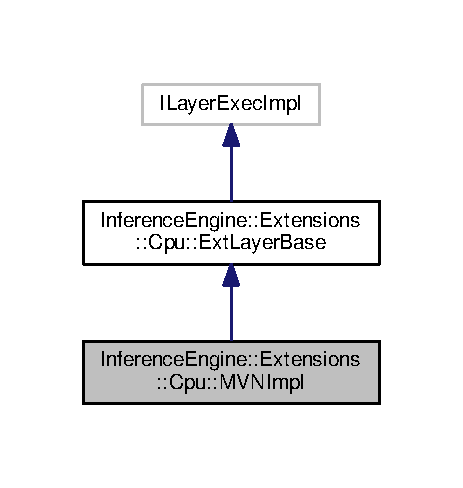
\includegraphics[width=222pt]{classInferenceEngine_1_1Extensions_1_1Cpu_1_1MVNImpl__inherit__graph}
\end{center}
\end{figure}


Collaboration diagram for Inference\+Engine\+:\+:Extensions\+:\+:Cpu\+:\+:M\+V\+N\+Impl\+:
\nopagebreak
\begin{figure}[H]
\begin{center}
\leavevmode
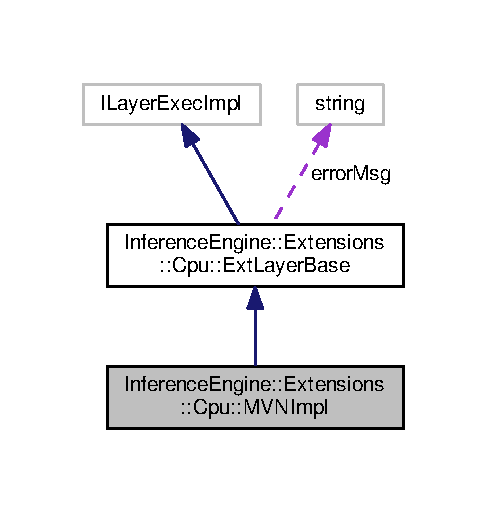
\includegraphics[width=234pt]{classInferenceEngine_1_1Extensions_1_1Cpu_1_1MVNImpl__coll__graph}
\end{center}
\end{figure}
\subsection*{Public Member Functions}
\begin{DoxyCompactItemize}
\item 
\hyperlink{classInferenceEngine_1_1Extensions_1_1Cpu_1_1MVNImpl_afbbb54c029bcfa2bfd204d55963438f0}{M\+V\+N\+Impl} (const C\+N\+N\+Layer $\ast$layer)
\item 
Status\+Code \hyperlink{classInferenceEngine_1_1Extensions_1_1Cpu_1_1MVNImpl_a654c2e29f3c9ce1e2c984de928a0441a}{execute} (std\+::vector$<$ Blob\+::\+Ptr $>$ \&inputs, std\+::vector$<$ Blob\+::\+Ptr $>$ \&outputs, Response\+Desc $\ast$resp) noexceptoverride
\end{DoxyCompactItemize}
\subsection*{Additional Inherited Members}


\subsection{Detailed Description}


Definition at line 28 of file ext\+\_\+mvn.\+cpp.



\subsection{Constructor \& Destructor Documentation}
\index{Inference\+Engine\+::\+Extensions\+::\+Cpu\+::\+M\+V\+N\+Impl@{Inference\+Engine\+::\+Extensions\+::\+Cpu\+::\+M\+V\+N\+Impl}!M\+V\+N\+Impl@{M\+V\+N\+Impl}}
\index{M\+V\+N\+Impl@{M\+V\+N\+Impl}!Inference\+Engine\+::\+Extensions\+::\+Cpu\+::\+M\+V\+N\+Impl@{Inference\+Engine\+::\+Extensions\+::\+Cpu\+::\+M\+V\+N\+Impl}}
\subsubsection[{\texorpdfstring{M\+V\+N\+Impl(const C\+N\+N\+Layer $\ast$layer)}{MVNImpl(const CNNLayer *layer)}}]{\setlength{\rightskip}{0pt plus 5cm}Inference\+Engine\+::\+Extensions\+::\+Cpu\+::\+M\+V\+N\+Impl\+::\+M\+V\+N\+Impl (
\begin{DoxyParamCaption}
\item[{const C\+N\+N\+Layer $\ast$}]{layer}
\end{DoxyParamCaption}
)\hspace{0.3cm}{\ttfamily [inline]}, {\ttfamily [explicit]}}\hypertarget{classInferenceEngine_1_1Extensions_1_1Cpu_1_1MVNImpl_afbbb54c029bcfa2bfd204d55963438f0}{}\label{classInferenceEngine_1_1Extensions_1_1Cpu_1_1MVNImpl_afbbb54c029bcfa2bfd204d55963438f0}


Definition at line 30 of file ext\+\_\+mvn.\+cpp.


\begin{DoxyCode}
30                                            : \hyperlink{classInferenceEngine_1_1Extensions_1_1Cpu_1_1ExtLayerBase_affff0e8263ca26852ccf71d299d7b06a}{ExtLayerBase}(layer) \{
31         \textcolor{keywordflow}{try} \{
32             \textcolor{keywordflow}{if} (\hyperlink{classInferenceEngine_1_1Extensions_1_1Cpu_1_1ExtLayerBase_a1074cdccacb9e9ca6eec01bbc2f7ca4a}{cnnLayer}.insData.size() != 1 || \hyperlink{classInferenceEngine_1_1Extensions_1_1Cpu_1_1ExtLayerBase_a1074cdccacb9e9ca6eec01bbc2f7ca4a}{cnnLayer}.outData.empty())
33                 THROW\_IE\_EXCEPTION << \textcolor{stringliteral}{"Incorrect number of input/output edges!"};
34 
35             across\_channels = \textcolor{keyword}{static\_cast<}\textcolor{keywordtype}{bool}\textcolor{keyword}{>}(\hyperlink{classInferenceEngine_1_1Extensions_1_1Cpu_1_1ExtLayerBase_a1074cdccacb9e9ca6eec01bbc2f7ca4a}{cnnLayer}.GetParamAsInt(\textcolor{stringliteral}{"across\_channels"}));
36             normalize\_variance = \textcolor{keyword}{static\_cast<}\textcolor{keywordtype}{bool}\textcolor{keyword}{>}(\hyperlink{classInferenceEngine_1_1Extensions_1_1Cpu_1_1ExtLayerBase_a1074cdccacb9e9ca6eec01bbc2f7ca4a}{cnnLayer}.GetParamAsInt(\textcolor{stringliteral}{"normalize\_variance"}));
37             eps = \hyperlink{classInferenceEngine_1_1Extensions_1_1Cpu_1_1ExtLayerBase_a1074cdccacb9e9ca6eec01bbc2f7ca4a}{cnnLayer}.GetParamAsFloat(\textcolor{stringliteral}{"eps"});
38 
39             \hyperlink{classInferenceEngine_1_1Extensions_1_1Cpu_1_1ExtLayerBase_a0ac7a6632e95b9500d5246b05b4b0bfa}{addConfig}(\{\{\hyperlink{classInferenceEngine_1_1Extensions_1_1Cpu_1_1ExtLayerBase_a1258a8d209e0249e0b1717618352ddfba446687ea2db1ada75be5ed053be77f59}{ConfLayout::PLN}, \textcolor{keyword}{false}, 0\}\}, \{\{
      \hyperlink{classInferenceEngine_1_1Extensions_1_1Cpu_1_1ExtLayerBase_a1258a8d209e0249e0b1717618352ddfba446687ea2db1ada75be5ed053be77f59}{ConfLayout::PLN}, \textcolor{keyword}{false}, 0\}\});
40         \} \textcolor{keywordflow}{catch} (InferenceEngine::details::InferenceEngineException &ex) \{
41             \hyperlink{classInferenceEngine_1_1Extensions_1_1Cpu_1_1ExtLayerBase_abc78e9b5a79fa339ffd831a5318f71f7}{errorMsg} = ex.what();
42         \}
43     \}
\end{DoxyCode}


\subsection{Member Function Documentation}
\index{Inference\+Engine\+::\+Extensions\+::\+Cpu\+::\+M\+V\+N\+Impl@{Inference\+Engine\+::\+Extensions\+::\+Cpu\+::\+M\+V\+N\+Impl}!execute@{execute}}
\index{execute@{execute}!Inference\+Engine\+::\+Extensions\+::\+Cpu\+::\+M\+V\+N\+Impl@{Inference\+Engine\+::\+Extensions\+::\+Cpu\+::\+M\+V\+N\+Impl}}
\subsubsection[{\texorpdfstring{execute(std\+::vector$<$ Blob\+::\+Ptr $>$ \&inputs, std\+::vector$<$ Blob\+::\+Ptr $>$ \&outputs, Response\+Desc $\ast$resp) noexceptoverride}{execute(std::vector< Blob::Ptr > &inputs, std::vector< Blob::Ptr > &outputs, ResponseDesc *resp) noexceptoverride}}]{\setlength{\rightskip}{0pt plus 5cm}Status\+Code Inference\+Engine\+::\+Extensions\+::\+Cpu\+::\+M\+V\+N\+Impl\+::execute (
\begin{DoxyParamCaption}
\item[{std\+::vector$<$ Blob\+::\+Ptr $>$ \&}]{inputs, }
\item[{std\+::vector$<$ Blob\+::\+Ptr $>$ \&}]{outputs, }
\item[{Response\+Desc $\ast$}]{resp}
\end{DoxyParamCaption}
)\hspace{0.3cm}{\ttfamily [inline]}, {\ttfamily [override]}, {\ttfamily [noexcept]}}\hypertarget{classInferenceEngine_1_1Extensions_1_1Cpu_1_1MVNImpl_a654c2e29f3c9ce1e2c984de928a0441a}{}\label{classInferenceEngine_1_1Extensions_1_1Cpu_1_1MVNImpl_a654c2e29f3c9ce1e2c984de928a0441a}


Definition at line 45 of file ext\+\_\+mvn.\+cpp.


\begin{DoxyCode}
46                                                              \{
47         \textcolor{keywordtype}{float}* src\_data = inputs[0]->buffer();
48         \textcolor{keywordtype}{float}* dst\_data = outputs[0]->buffer();
49 
50         SizeVector dims = inputs[0]->getTensorDesc().getDims();
51 
52         \textcolor{keywordtype}{int} N = \textcolor{keyword}{static\_cast<}\textcolor{keywordtype}{int}\textcolor{keyword}{>}((dims.size() > 0) ? dims[0] : 1);
53         \textcolor{keywordtype}{int} C = \textcolor{keyword}{static\_cast<}\textcolor{keywordtype}{int}\textcolor{keyword}{>}((dims.size() > 1) ? dims[1] : 1);
54         \textcolor{keywordtype}{int} H = \textcolor{keyword}{static\_cast<}\textcolor{keywordtype}{int}\textcolor{keyword}{>}((dims.size() > 2) ? dims[2] : 1);
55         \textcolor{keywordtype}{int} W = \textcolor{keyword}{static\_cast<}\textcolor{keywordtype}{int}\textcolor{keyword}{>}((dims.size() > 3) ? dims[3] : 1);
56 
57         \textcolor{keywordflow}{for} (\textcolor{keywordtype}{int} b = 0; b < N; b++) \{
58             \textcolor{comment}{// Calculate mean value}
59             \textcolor{keywordflow}{if} (across\_channels) \{
60                 \textcolor{keywordtype}{double} mean = 0;
61 \textcolor{preprocessor}{                #pragma omp parallel for reduction(+ : mean) schedule(static)}
62                 \textcolor{keywordflow}{for} (\textcolor{keywordtype}{int} \hyperlink{CMakeCache_8txt_aac1d6a1710812201527c735f7c6afbaa}{c} = 0; \hyperlink{CMakeCache_8txt_aac1d6a1710812201527c735f7c6afbaa}{c} < C; \hyperlink{CMakeCache_8txt_aac1d6a1710812201527c735f7c6afbaa}{c}++) \{
63                     \textcolor{keywordflow}{for} (\textcolor{keywordtype}{int} h = 0; h < H; h++) \{
64                         \textcolor{keywordflow}{for} (\textcolor{keywordtype}{int} w = 0; w < W; w++) \{
65                             mean += src\_data[b*C*H*W + \hyperlink{CMakeCache_8txt_aac1d6a1710812201527c735f7c6afbaa}{c}*H*W + h*W + w];
66                         \}
67                     \}
68                 \}
69                 mean /= C*H*W;
70 \textcolor{preprocessor}{                #pragma omp parallel for schedule(static)}
71                 \textcolor{keywordflow}{for} (\textcolor{keywordtype}{int} \hyperlink{CMakeCache_8txt_aac1d6a1710812201527c735f7c6afbaa}{c} = 0; \hyperlink{CMakeCache_8txt_aac1d6a1710812201527c735f7c6afbaa}{c} < C; \hyperlink{CMakeCache_8txt_aac1d6a1710812201527c735f7c6afbaa}{c}++) \{
72                     \textcolor{keywordflow}{for} (\textcolor{keywordtype}{int} h = 0; h < H; h++) \{
73                         \textcolor{keywordflow}{for} (\textcolor{keywordtype}{int} w = 0; w < W; w++) \{
74                             dst\_data[b*C*H*W + \hyperlink{CMakeCache_8txt_aac1d6a1710812201527c735f7c6afbaa}{c}*H*W + h*W + w] = src\_data[b*C*H*W + 
      \hyperlink{CMakeCache_8txt_aac1d6a1710812201527c735f7c6afbaa}{c}*H*W + h*W + w] - mean;
75                         \}
76                     \}
77                 \}
78             \} \textcolor{keywordflow}{else} \{
79 \textcolor{preprocessor}{                #pragma omp parallel for schedule(static)}
80                 \textcolor{keywordflow}{for} (\textcolor{keywordtype}{int} \hyperlink{CMakeCache_8txt_aac1d6a1710812201527c735f7c6afbaa}{c} = 0; \hyperlink{CMakeCache_8txt_aac1d6a1710812201527c735f7c6afbaa}{c} < C; \hyperlink{CMakeCache_8txt_aac1d6a1710812201527c735f7c6afbaa}{c}++) \{
81                     \textcolor{keywordtype}{double} mean = 0;
82                     \textcolor{keywordflow}{for} (\textcolor{keywordtype}{int} h = 0; h < H; h++) \{
83                         \textcolor{keywordflow}{for} (\textcolor{keywordtype}{int} w = 0; w < W; w++) \{
84                             mean += src\_data[b*C*H*W + \hyperlink{CMakeCache_8txt_aac1d6a1710812201527c735f7c6afbaa}{c}*H*W + h*W + w];
85                         \}
86                     \}
87                     mean /= H*W;
88 
89                     \textcolor{keywordflow}{for} (\textcolor{keywordtype}{int} h = 0; h < H; h++) \{
90                         \textcolor{keywordflow}{for} (\textcolor{keywordtype}{int} w = 0; w < W; w++) \{
91                             dst\_data[b*C*H*W + \hyperlink{CMakeCache_8txt_aac1d6a1710812201527c735f7c6afbaa}{c}*H*W + h*W + w] = src\_data[b*C*H*W + 
      \hyperlink{CMakeCache_8txt_aac1d6a1710812201527c735f7c6afbaa}{c}*H*W + h*W + w] - mean;
92                         \}
93                     \}
94                 \}
95             \}
96         \}
97 
98         \textcolor{keywordflow}{if} (normalize\_variance) \{
99             \textcolor{keywordflow}{for} (\textcolor{keywordtype}{int} b = 0; b < N; b++) \{
100                 \textcolor{comment}{// Calculate variances value}
101                 \textcolor{keywordflow}{if} (across\_channels) \{
102                     \textcolor{keywordtype}{double} variance = 0;
103 \textcolor{preprocessor}{                    #pragma omp parallel for reduction(+ : variance) schedule(static)}
104                     \textcolor{keywordflow}{for} (\textcolor{keywordtype}{int} \hyperlink{CMakeCache_8txt_aac1d6a1710812201527c735f7c6afbaa}{c} = 0; \hyperlink{CMakeCache_8txt_aac1d6a1710812201527c735f7c6afbaa}{c} < C; \hyperlink{CMakeCache_8txt_aac1d6a1710812201527c735f7c6afbaa}{c}++) \{
105                         \textcolor{keywordflow}{for} (\textcolor{keywordtype}{int} h = 0; h < H; h++) \{
106                             \textcolor{keywordflow}{for} (\textcolor{keywordtype}{int} w = 0; w < W; w++) \{
107                                 variance += std::pow(dst\_data[b*C*H*W + \hyperlink{CMakeCache_8txt_aac1d6a1710812201527c735f7c6afbaa}{c}*H*W + h*W + w], 2);
108                             \}
109                         \}
110                     \}
111                     variance /= C*H*W;
112                     variance = std::pow(variance, 0.5f);
113                     variance += eps;
114 \textcolor{preprocessor}{                    #pragma omp parallel for schedule(static)}
115                     \textcolor{keywordflow}{for} (\textcolor{keywordtype}{int} \hyperlink{CMakeCache_8txt_aac1d6a1710812201527c735f7c6afbaa}{c} = 0; \hyperlink{CMakeCache_8txt_aac1d6a1710812201527c735f7c6afbaa}{c} < C; \hyperlink{CMakeCache_8txt_aac1d6a1710812201527c735f7c6afbaa}{c}++) \{
116                         \textcolor{keywordflow}{for} (\textcolor{keywordtype}{int} h = 0; h < H; h++) \{
117                             \textcolor{keywordflow}{for} (\textcolor{keywordtype}{int} w = 0; w < W; w++) \{
118                                 dst\_data[b*C*H*W + \hyperlink{CMakeCache_8txt_aac1d6a1710812201527c735f7c6afbaa}{c}*H*W + h*W + w] /= variance;
119                             \}
120                         \}
121                     \}
122                 \} \textcolor{keywordflow}{else} \{
123 \textcolor{preprocessor}{                    #pragma omp parallel for schedule(static)}
124                     \textcolor{keywordflow}{for} (\textcolor{keywordtype}{int} \hyperlink{CMakeCache_8txt_aac1d6a1710812201527c735f7c6afbaa}{c} = 0; \hyperlink{CMakeCache_8txt_aac1d6a1710812201527c735f7c6afbaa}{c} < C; \hyperlink{CMakeCache_8txt_aac1d6a1710812201527c735f7c6afbaa}{c}++) \{
125                         \textcolor{keywordtype}{double} variance = 0;
126                         \textcolor{keywordflow}{for} (\textcolor{keywordtype}{int} h = 0; h < H; h++) \{
127                             \textcolor{keywordflow}{for} (\textcolor{keywordtype}{int} w = 0; w < W; w++) \{
128                                 variance += std::pow(dst\_data[b*C*H*W + \hyperlink{CMakeCache_8txt_aac1d6a1710812201527c735f7c6afbaa}{c}*H*W + h*W + w], 2);
129                             \}
130                         \}
131                         variance /= H*W;
132                         variance = std::pow(variance, 0.5f);
133                         variance += eps;
134                         \textcolor{keywordflow}{for} (\textcolor{keywordtype}{int} h = 0; h < H; h++) \{
135                             \textcolor{keywordflow}{for} (\textcolor{keywordtype}{int} w = 0; w < W; w++) \{
136                                 dst\_data[b*C*H*W + \hyperlink{CMakeCache_8txt_aac1d6a1710812201527c735f7c6afbaa}{c}*H*W + h*W + w] /= variance;
137                             \}
138                         \}
139                     \}
140                 \}
141             \}
142         \}
143         \textcolor{keywordflow}{return} OK;
144     \}
\end{DoxyCode}


The documentation for this class was generated from the following file\+:\begin{DoxyCompactItemize}
\item 
thirdparty/extension/\hyperlink{ext__mvn_8cpp}{ext\+\_\+mvn.\+cpp}\end{DoxyCompactItemize}

\hypertarget{classNetworkEngine}{}\section{Network\+Engine Class Reference}
\label{classNetworkEngine}\index{Network\+Engine@{Network\+Engine}}


This class is used to get the infer request from a inference plugin and an inference network.  




{\ttfamily \#include $<$engine.\+h$>$}

\subsection*{Public Member Functions}
\begin{DoxyCompactItemize}
\item 
\hyperlink{classNetworkEngine_a7529534aa07732f4efe7ec7f68dd9c01}{Network\+Engine} (Inference\+Engine\+::\+Inference\+Plugin $\ast$, const \hyperlink{classValidatedBaseNetwork}{Validated\+Base\+Network} \&)
\begin{DoxyCompactList}\small\item\em Create an \hyperlink{classNetworkEngine}{Network\+Engine} instance from a inference plugin and an inference network. \end{DoxyCompactList}\item 
Inference\+Engine\+::\+Infer\+Request\+::\+Ptr \& \hyperlink{classNetworkEngine_af5f24575f4110047bb7566e8b8f76006}{get\+Request} ()
\begin{DoxyCompactList}\small\item\em Get the inference request this instance holds. \end{DoxyCompactList}\item 
{\footnotesize template$<$typename T $>$ }\\void \hyperlink{classNetworkEngine_a76660bfd6bee75bd2e83a28751e00f2c}{set\+Completion\+Callback} (const T \&callback\+To\+Set)
\begin{DoxyCompactList}\small\item\em Set a callback function for the infer request. \end{DoxyCompactList}\end{DoxyCompactItemize}


\subsection{Detailed Description}
This class is used to get the infer request from a inference plugin and an inference network. 

Definition at line 18 of file engine.\+h.



\subsection{Constructor \& Destructor Documentation}
\index{Network\+Engine@{Network\+Engine}!Network\+Engine@{Network\+Engine}}
\index{Network\+Engine@{Network\+Engine}!Network\+Engine@{Network\+Engine}}
\subsubsection[{\texorpdfstring{Network\+Engine(\+Inference\+Engine\+::\+Inference\+Plugin $\ast$, const Validated\+Base\+Network \&)}{NetworkEngine(InferenceEngine::InferencePlugin *, const ValidatedBaseNetwork &)}}]{\setlength{\rightskip}{0pt plus 5cm}Network\+Engine\+::\+Network\+Engine (
\begin{DoxyParamCaption}
\item[{Inference\+Engine\+::\+Inference\+Plugin $\ast$}]{plg, }
\item[{const {\bf Validated\+Base\+Network} \&}]{validated\+\_\+network}
\end{DoxyParamCaption}
)}\hypertarget{classNetworkEngine_a7529534aa07732f4efe7ec7f68dd9c01}{}\label{classNetworkEngine_a7529534aa07732f4efe7ec7f68dd9c01}


Create an \hyperlink{classNetworkEngine}{Network\+Engine} instance from a inference plugin and an inference network. 



Definition at line 7 of file engine.\+cpp.


\begin{DoxyCode}
9                                                     \{
10   request\_ = (plg->LoadNetwork(validated\_network.net\_reader\_->getNetwork(), \{\}))
11       .CreateInferRequestPtr();
12 \}\end{DoxyCode}


\subsection{Member Function Documentation}
\index{Network\+Engine@{Network\+Engine}!get\+Request@{get\+Request}}
\index{get\+Request@{get\+Request}!Network\+Engine@{Network\+Engine}}
\subsubsection[{\texorpdfstring{get\+Request()}{getRequest()}}]{\setlength{\rightskip}{0pt plus 5cm}Inference\+Engine\+::\+Infer\+Request\+::\+Ptr\& Network\+Engine\+::get\+Request (
\begin{DoxyParamCaption}
{}
\end{DoxyParamCaption}
)\hspace{0.3cm}{\ttfamily [inline]}}\hypertarget{classNetworkEngine_af5f24575f4110047bb7566e8b8f76006}{}\label{classNetworkEngine_af5f24575f4110047bb7566e8b8f76006}


Get the inference request this instance holds. 



Definition at line 29 of file engine.\+h.


\begin{DoxyCode}
29 \{ \textcolor{keywordflow}{return} request\_; \}
\end{DoxyCode}
\index{Network\+Engine@{Network\+Engine}!set\+Completion\+Callback@{set\+Completion\+Callback}}
\index{set\+Completion\+Callback@{set\+Completion\+Callback}!Network\+Engine@{Network\+Engine}}
\subsubsection[{\texorpdfstring{set\+Completion\+Callback(const T \&callback\+To\+Set)}{setCompletionCallback(const T &callbackToSet)}}]{\setlength{\rightskip}{0pt plus 5cm}template$<$typename T $>$ void Network\+Engine\+::set\+Completion\+Callback (
\begin{DoxyParamCaption}
\item[{const T \&}]{callback\+To\+Set}
\end{DoxyParamCaption}
)\hspace{0.3cm}{\ttfamily [inline]}}\hypertarget{classNetworkEngine_a76660bfd6bee75bd2e83a28751e00f2c}{}\label{classNetworkEngine_a76660bfd6bee75bd2e83a28751e00f2c}


Set a callback function for the infer request. 


\begin{DoxyParams}[1]{Parameters}
\mbox{\tt in}  & {\em callback\+To\+Set} & A lambda function as callback function. The callback function will be called when request is finished. \\
\hline
\end{DoxyParams}


Definition at line 36 of file engine.\+h.


\begin{DoxyCode}
36                                                       \{
37     request\_->SetCompletionCallback(callbackToSet);
38   \}
\end{DoxyCode}


The documentation for this class was generated from the following files\+:\begin{DoxyCompactItemize}
\item 
include/openvino\+\_\+service/engines/\hyperlink{engine_8h}{engine.\+h}\item 
lib/engines/\hyperlink{engine_8cpp}{engine.\+cpp}\end{DoxyCompactItemize}

\hypertarget{classInferenceEngine_1_1Extensions_1_1Cpu_1_1NormalizeFactory}{}\section{Inference\+Engine\+:\+:Extensions\+:\+:Cpu\+:\+:Normalize\+Factory Class Reference}
\label{classInferenceEngine_1_1Extensions_1_1Cpu_1_1NormalizeFactory}\index{Inference\+Engine\+::\+Extensions\+::\+Cpu\+::\+Normalize\+Factory@{Inference\+Engine\+::\+Extensions\+::\+Cpu\+::\+Normalize\+Factory}}


Inheritance diagram for Inference\+Engine\+:\+:Extensions\+:\+:Cpu\+:\+:Normalize\+Factory\+:
\nopagebreak
\begin{figure}[H]
\begin{center}
\leavevmode
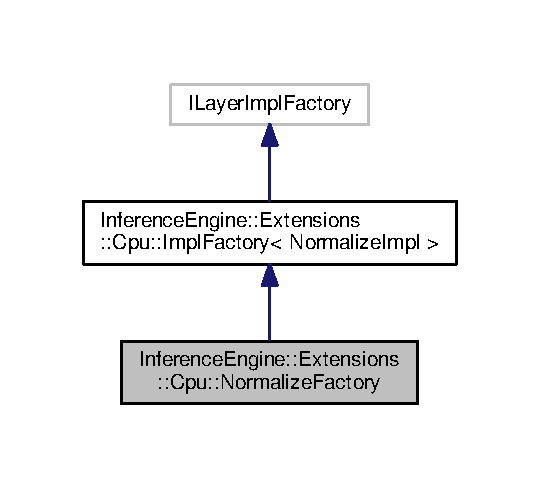
\includegraphics[width=259pt]{classInferenceEngine_1_1Extensions_1_1Cpu_1_1NormalizeFactory__inherit__graph}
\end{center}
\end{figure}


Collaboration diagram for Inference\+Engine\+:\+:Extensions\+:\+:Cpu\+:\+:Normalize\+Factory\+:
\nopagebreak
\begin{figure}[H]
\begin{center}
\leavevmode
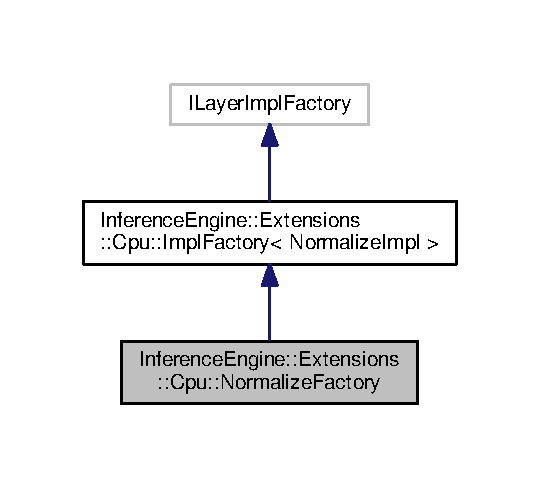
\includegraphics[width=259pt]{classInferenceEngine_1_1Extensions_1_1Cpu_1_1NormalizeFactory__coll__graph}
\end{center}
\end{figure}
\subsection*{Public Member Functions}
\begin{DoxyCompactItemize}
\item 
\hyperlink{classInferenceEngine_1_1Extensions_1_1Cpu_1_1NormalizeFactory_a0c60630da765a5314dec1c7251fd52b8}{Normalize\+Factory} (const C\+N\+N\+Layer $\ast$layer)
\item 
Status\+Code \hyperlink{classInferenceEngine_1_1Extensions_1_1Cpu_1_1NormalizeFactory_a2fefa3e07b9ddf93a9a7c3e418e3fc0e}{get\+Shapes} (const std\+::vector$<$ Tensor\+Desc $>$ \&in\+Shapes, std\+::vector$<$ Tensor\+Desc $>$ \&out\+Shapes, Response\+Desc $\ast$resp) noexceptoverride
\end{DoxyCompactItemize}
\subsection*{Additional Inherited Members}


\subsection{Detailed Description}


Definition at line 232 of file ext\+\_\+normalize.\+cpp.



\subsection{Constructor \& Destructor Documentation}
\index{Inference\+Engine\+::\+Extensions\+::\+Cpu\+::\+Normalize\+Factory@{Inference\+Engine\+::\+Extensions\+::\+Cpu\+::\+Normalize\+Factory}!Normalize\+Factory@{Normalize\+Factory}}
\index{Normalize\+Factory@{Normalize\+Factory}!Inference\+Engine\+::\+Extensions\+::\+Cpu\+::\+Normalize\+Factory@{Inference\+Engine\+::\+Extensions\+::\+Cpu\+::\+Normalize\+Factory}}
\subsubsection[{\texorpdfstring{Normalize\+Factory(const C\+N\+N\+Layer $\ast$layer)}{NormalizeFactory(const CNNLayer *layer)}}]{\setlength{\rightskip}{0pt plus 5cm}Inference\+Engine\+::\+Extensions\+::\+Cpu\+::\+Normalize\+Factory\+::\+Normalize\+Factory (
\begin{DoxyParamCaption}
\item[{const C\+N\+N\+Layer $\ast$}]{layer}
\end{DoxyParamCaption}
)\hspace{0.3cm}{\ttfamily [inline]}, {\ttfamily [explicit]}}\hypertarget{classInferenceEngine_1_1Extensions_1_1Cpu_1_1NormalizeFactory_a0c60630da765a5314dec1c7251fd52b8}{}\label{classInferenceEngine_1_1Extensions_1_1Cpu_1_1NormalizeFactory_a0c60630da765a5314dec1c7251fd52b8}


Definition at line 234 of file ext\+\_\+normalize.\+cpp.


\begin{DoxyCode}
234 : \hyperlink{classInferenceEngine_1_1Extensions_1_1Cpu_1_1ImplFactory_a86837f88ce5c196382c1f7c38e3ba3a8}{ImplFactory}(layer) \{\}
\end{DoxyCode}


\subsection{Member Function Documentation}
\index{Inference\+Engine\+::\+Extensions\+::\+Cpu\+::\+Normalize\+Factory@{Inference\+Engine\+::\+Extensions\+::\+Cpu\+::\+Normalize\+Factory}!get\+Shapes@{get\+Shapes}}
\index{get\+Shapes@{get\+Shapes}!Inference\+Engine\+::\+Extensions\+::\+Cpu\+::\+Normalize\+Factory@{Inference\+Engine\+::\+Extensions\+::\+Cpu\+::\+Normalize\+Factory}}
\subsubsection[{\texorpdfstring{get\+Shapes(const std\+::vector$<$ Tensor\+Desc $>$ \&in\+Shapes, std\+::vector$<$ Tensor\+Desc $>$ \&out\+Shapes, Response\+Desc $\ast$resp) noexceptoverride}{getShapes(const std::vector< TensorDesc > &inShapes, std::vector< TensorDesc > &outShapes, ResponseDesc *resp) noexceptoverride}}]{\setlength{\rightskip}{0pt plus 5cm}Status\+Code Inference\+Engine\+::\+Extensions\+::\+Cpu\+::\+Normalize\+Factory\+::get\+Shapes (
\begin{DoxyParamCaption}
\item[{const std\+::vector$<$ Tensor\+Desc $>$ \&}]{in\+Shapes, }
\item[{std\+::vector$<$ Tensor\+Desc $>$ \&}]{out\+Shapes, }
\item[{Response\+Desc $\ast$}]{resp}
\end{DoxyParamCaption}
)\hspace{0.3cm}{\ttfamily [inline]}, {\ttfamily [override]}, {\ttfamily [noexcept]}}\hypertarget{classInferenceEngine_1_1Extensions_1_1Cpu_1_1NormalizeFactory_a2fefa3e07b9ddf93a9a7c3e418e3fc0e}{}\label{classInferenceEngine_1_1Extensions_1_1Cpu_1_1NormalizeFactory_a2fefa3e07b9ddf93a9a7c3e418e3fc0e}


Definition at line 236 of file ext\+\_\+normalize.\+cpp.


\begin{DoxyCode}
237                                                                \{
238         outShapes.push\_back(inShapes[0]);
239         \textcolor{keywordflow}{return} InferenceEngine::OK;
240     \}
\end{DoxyCode}


The documentation for this class was generated from the following file\+:\begin{DoxyCompactItemize}
\item 
thirdparty/extension/\hyperlink{ext__normalize_8cpp}{ext\+\_\+normalize.\+cpp}\end{DoxyCompactItemize}

\hypertarget{classInferenceEngine_1_1Extensions_1_1Cpu_1_1NormalizeImpl}{}\section{Inference\+Engine\+:\+:Extensions\+:\+:Cpu\+:\+:Normalize\+Impl Class Reference}
\label{classInferenceEngine_1_1Extensions_1_1Cpu_1_1NormalizeImpl}\index{Inference\+Engine\+::\+Extensions\+::\+Cpu\+::\+Normalize\+Impl@{Inference\+Engine\+::\+Extensions\+::\+Cpu\+::\+Normalize\+Impl}}


Inheritance diagram for Inference\+Engine\+:\+:Extensions\+:\+:Cpu\+:\+:Normalize\+Impl\+:
\nopagebreak
\begin{figure}[H]
\begin{center}
\leavevmode
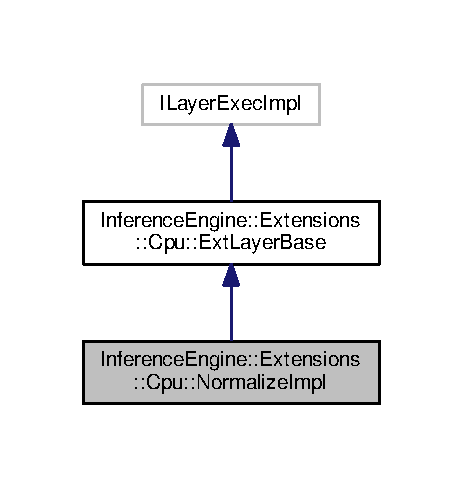
\includegraphics[width=222pt]{classInferenceEngine_1_1Extensions_1_1Cpu_1_1NormalizeImpl__inherit__graph}
\end{center}
\end{figure}


Collaboration diagram for Inference\+Engine\+:\+:Extensions\+:\+:Cpu\+:\+:Normalize\+Impl\+:
\nopagebreak
\begin{figure}[H]
\begin{center}
\leavevmode
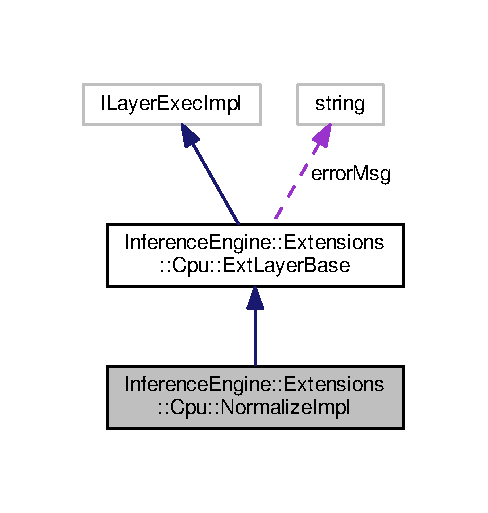
\includegraphics[width=234pt]{classInferenceEngine_1_1Extensions_1_1Cpu_1_1NormalizeImpl__coll__graph}
\end{center}
\end{figure}
\subsection*{Public Member Functions}
\begin{DoxyCompactItemize}
\item 
\hyperlink{classInferenceEngine_1_1Extensions_1_1Cpu_1_1NormalizeImpl_a45024d9af0dc5579efdc2b8660cb4c17}{Normalize\+Impl} (const C\+N\+N\+Layer $\ast$layer)
\item 
Status\+Code \hyperlink{classInferenceEngine_1_1Extensions_1_1Cpu_1_1NormalizeImpl_a912719712bd31cb88fbb02b884ee33c5}{execute} (std\+::vector$<$ Blob\+::\+Ptr $>$ \&inputs, std\+::vector$<$ Blob\+::\+Ptr $>$ \&outputs, Response\+Desc $\ast$resp) noexceptoverride
\end{DoxyCompactItemize}
\subsection*{Additional Inherited Members}


\subsection{Detailed Description}


Definition at line 30 of file ext\+\_\+normalize.\+cpp.



\subsection{Constructor \& Destructor Documentation}
\index{Inference\+Engine\+::\+Extensions\+::\+Cpu\+::\+Normalize\+Impl@{Inference\+Engine\+::\+Extensions\+::\+Cpu\+::\+Normalize\+Impl}!Normalize\+Impl@{Normalize\+Impl}}
\index{Normalize\+Impl@{Normalize\+Impl}!Inference\+Engine\+::\+Extensions\+::\+Cpu\+::\+Normalize\+Impl@{Inference\+Engine\+::\+Extensions\+::\+Cpu\+::\+Normalize\+Impl}}
\subsubsection[{\texorpdfstring{Normalize\+Impl(const C\+N\+N\+Layer $\ast$layer)}{NormalizeImpl(const CNNLayer *layer)}}]{\setlength{\rightskip}{0pt plus 5cm}Inference\+Engine\+::\+Extensions\+::\+Cpu\+::\+Normalize\+Impl\+::\+Normalize\+Impl (
\begin{DoxyParamCaption}
\item[{const C\+N\+N\+Layer $\ast$}]{layer}
\end{DoxyParamCaption}
)\hspace{0.3cm}{\ttfamily [inline]}, {\ttfamily [explicit]}}\hypertarget{classInferenceEngine_1_1Extensions_1_1Cpu_1_1NormalizeImpl_a45024d9af0dc5579efdc2b8660cb4c17}{}\label{classInferenceEngine_1_1Extensions_1_1Cpu_1_1NormalizeImpl_a45024d9af0dc5579efdc2b8660cb4c17}


Definition at line 32 of file ext\+\_\+normalize.\+cpp.


\begin{DoxyCode}
32                                                  : \hyperlink{classInferenceEngine_1_1Extensions_1_1Cpu_1_1ExtLayerBase_affff0e8263ca26852ccf71d299d7b06a}{ExtLayerBase}(layer) \{
33         \textcolor{keywordflow}{try} \{
34             \textcolor{keywordflow}{if} (\hyperlink{classInferenceEngine_1_1Extensions_1_1Cpu_1_1ExtLayerBase_a1074cdccacb9e9ca6eec01bbc2f7ca4a}{cnnLayer}.insData.size() != 1 || \hyperlink{classInferenceEngine_1_1Extensions_1_1Cpu_1_1ExtLayerBase_a1074cdccacb9e9ca6eec01bbc2f7ca4a}{cnnLayer}.outData.size() != 1)
35                 THROW\_IE\_EXCEPTION << \textcolor{stringliteral}{"Incorrect number of input/output edges!"};
36 
37             weights = std::dynamic\_pointer\_cast<TBlob<float>>(\hyperlink{classInferenceEngine_1_1Extensions_1_1Cpu_1_1ExtLayerBase_a1074cdccacb9e9ca6eec01bbc2f7ca4a}{cnnLayer}.blobs[\textcolor{stringliteral}{"weights"}]);
38             \textcolor{keywordflow}{if} (!weights)
39                 THROW\_IE\_EXCEPTION << \hyperlink{classInferenceEngine_1_1Extensions_1_1Cpu_1_1ExtLayerBase_a1074cdccacb9e9ca6eec01bbc2f7ca4a}{cnnLayer}.name << \textcolor{stringliteral}{" weights is empty!"};
40             across\_spatial = \textcolor{keyword}{static\_cast<}\textcolor{keywordtype}{bool}\textcolor{keyword}{>}(\hyperlink{classInferenceEngine_1_1Extensions_1_1Cpu_1_1ExtLayerBase_a1074cdccacb9e9ca6eec01bbc2f7ca4a}{cnnLayer}.GetParamAsInt(\textcolor{stringliteral}{"across\_spatial"}));
41             channel\_shared = \textcolor{keyword}{static\_cast<}\textcolor{keywordtype}{bool}\textcolor{keyword}{>}(\hyperlink{classInferenceEngine_1_1Extensions_1_1Cpu_1_1ExtLayerBase_a1074cdccacb9e9ca6eec01bbc2f7ca4a}{cnnLayer}.GetParamAsInt(\textcolor{stringliteral}{"channel\_shared"}));
42             eps = \hyperlink{classInferenceEngine_1_1Extensions_1_1Cpu_1_1ExtLayerBase_a1074cdccacb9e9ca6eec01bbc2f7ca4a}{cnnLayer}.GetParamAsFloat(\textcolor{stringliteral}{"eps"});
43 
44             \hyperlink{classInferenceEngine_1_1Extensions_1_1Cpu_1_1ExtLayerBase_a0ac7a6632e95b9500d5246b05b4b0bfa}{addConfig}(\{\{\hyperlink{classInferenceEngine_1_1Extensions_1_1Cpu_1_1ExtLayerBase_a1258a8d209e0249e0b1717618352ddfba446687ea2db1ada75be5ed053be77f59}{ConfLayout::PLN}, \textcolor{keyword}{false}, 0\}\}, \{\{
      \hyperlink{classInferenceEngine_1_1Extensions_1_1Cpu_1_1ExtLayerBase_a1258a8d209e0249e0b1717618352ddfba446687ea2db1ada75be5ed053be77f59}{ConfLayout::PLN}, \textcolor{keyword}{false}, 0\}\}, \textcolor{keyword}{true});
45         \} \textcolor{keywordflow}{catch} (InferenceEngine::details::InferenceEngineException &ex) \{
46             \hyperlink{classInferenceEngine_1_1Extensions_1_1Cpu_1_1ExtLayerBase_abc78e9b5a79fa339ffd831a5318f71f7}{errorMsg} = ex.what();
47         \}
48     \}
\end{DoxyCode}


\subsection{Member Function Documentation}
\index{Inference\+Engine\+::\+Extensions\+::\+Cpu\+::\+Normalize\+Impl@{Inference\+Engine\+::\+Extensions\+::\+Cpu\+::\+Normalize\+Impl}!execute@{execute}}
\index{execute@{execute}!Inference\+Engine\+::\+Extensions\+::\+Cpu\+::\+Normalize\+Impl@{Inference\+Engine\+::\+Extensions\+::\+Cpu\+::\+Normalize\+Impl}}
\subsubsection[{\texorpdfstring{execute(std\+::vector$<$ Blob\+::\+Ptr $>$ \&inputs, std\+::vector$<$ Blob\+::\+Ptr $>$ \&outputs, Response\+Desc $\ast$resp) noexceptoverride}{execute(std::vector< Blob::Ptr > &inputs, std::vector< Blob::Ptr > &outputs, ResponseDesc *resp) noexceptoverride}}]{\setlength{\rightskip}{0pt plus 5cm}Status\+Code Inference\+Engine\+::\+Extensions\+::\+Cpu\+::\+Normalize\+Impl\+::execute (
\begin{DoxyParamCaption}
\item[{std\+::vector$<$ Blob\+::\+Ptr $>$ \&}]{inputs, }
\item[{std\+::vector$<$ Blob\+::\+Ptr $>$ \&}]{outputs, }
\item[{Response\+Desc $\ast$}]{resp}
\end{DoxyParamCaption}
)\hspace{0.3cm}{\ttfamily [inline]}, {\ttfamily [override]}, {\ttfamily [noexcept]}}\hypertarget{classInferenceEngine_1_1Extensions_1_1Cpu_1_1NormalizeImpl_a912719712bd31cb88fbb02b884ee33c5}{}\label{classInferenceEngine_1_1Extensions_1_1Cpu_1_1NormalizeImpl_a912719712bd31cb88fbb02b884ee33c5}


Definition at line 72 of file ext\+\_\+normalize.\+cpp.


\begin{DoxyCode}
73                                                              \{
74         \textcolor{keywordflow}{if} (inputs.size() != 1 || outputs.empty()) \{
75             \textcolor{keywordflow}{if} (resp) \{
76                 std::string \hyperlink{classInferenceEngine_1_1Extensions_1_1Cpu_1_1ExtLayerBase_abc78e9b5a79fa339ffd831a5318f71f7}{errorMsg} = \textcolor{stringliteral}{"Incorrect number of input or output edges!"};
77                 errorMsg.copy(resp->msg, \textcolor{keyword}{sizeof}(resp->msg) - 1);
78             \}
79             \textcolor{keywordflow}{return} GENERAL\_ERROR;
80         \}
81         \textcolor{keyword}{const} \textcolor{keywordtype}{float}* src = inputs[0]->buffer();
82         \textcolor{keyword}{const} \textcolor{keywordtype}{float}* scl = weights->buffer();
83         \textcolor{keywordtype}{float}* dst = outputs[0]->buffer();
84 
85         SizeVector dims = inputs[0]->getTensorDesc().getDims();
86 
87         \textcolor{keyword}{const} \textcolor{keywordtype}{int} N = \textcolor{keyword}{static\_cast<}\textcolor{keyword}{const }\textcolor{keywordtype}{int}\textcolor{keyword}{>}(dims[0]);
88         \textcolor{keyword}{const} \textcolor{keywordtype}{int} C = \textcolor{keyword}{static\_cast<}\textcolor{keywordtype}{int}\textcolor{keyword}{>}(dims[1]);
89         \textcolor{keyword}{const} \textcolor{keywordtype}{int} H = \textcolor{keyword}{static\_cast<}\textcolor{keywordtype}{int}\textcolor{keyword}{>}(dims[2]);
90         \textcolor{keyword}{const} \textcolor{keywordtype}{int} W = \textcolor{keyword}{static\_cast<}\textcolor{keywordtype}{int}\textcolor{keyword}{>}(dims[3]);
91 
92         \textcolor{keyword}{const} \textcolor{keywordtype}{int} HW = H*W;
93         \textcolor{keyword}{const} \textcolor{keywordtype}{int} CHW = C*HW;
94 
95         \textcolor{keywordflow}{for} (\textcolor{keywordtype}{int} n = 0; n < N; n++) \{
96             \textcolor{keyword}{const} \textcolor{keywordtype}{float}* psrc = src + n*C*H*W;
97             \textcolor{keywordtype}{float}* pdst = dst + n*C*H*W;
98 
99             \textcolor{keywordflow}{if} (across\_spatial) \{
100                 \textcolor{keywordtype}{float} norm = eps;
101                 \textcolor{keywordtype}{int} i = 0;
102 \textcolor{preprocessor}{#if defined(HAVE\_AVX2)}
103                 \{
104                     \_\_m256 vsum = \_mm256\_setzero\_ps();
105                     \textcolor{keywordflow}{for} (; i <= C*H*W-8; i += 8) \{
106                         \_\_m256 vsrc = \_mm256\_loadu\_ps(psrc + i);
107                         vsum = \_mm256\_fmadd\_ps(vsrc, vsrc, vsum);
108                     \}
109                     norm += hsum\_avx2(vsum);
110                 \}
111 \textcolor{preprocessor}{#elif defined(HAVE\_SSE)}
112                 \{
113                     \_\_m128 vsum = \_mm\_setzero\_ps();
114                     \textcolor{keywordflow}{for} (; i <= C*H*W-4; i += 4) \{
115                         \_\_m128 vsrc = \_mm\_loadu\_ps(psrc + i);
116                         vsum = \_mm\_add\_ps(\_mm\_mul\_ps(vsrc, vsrc), vsum);
117                     \}
118                     norm += hsum\_sse(vsum);
119                 \}
120 \textcolor{preprocessor}{#endif}
121                 \textcolor{keywordflow}{for} (; i < C*H*W; i++) \{
122                     norm += psrc[i]*psrc[i];
123                 \}
124                 norm = 1.0f / std::sqrt(norm);
125 
126                 \textcolor{keywordflow}{for} (\textcolor{keywordtype}{int} \hyperlink{CMakeCache_8txt_aac1d6a1710812201527c735f7c6afbaa}{c} = 0 ; \hyperlink{CMakeCache_8txt_aac1d6a1710812201527c735f7c6afbaa}{c} < C; \hyperlink{CMakeCache_8txt_aac1d6a1710812201527c735f7c6afbaa}{c}++) \{
127                     \textcolor{keywordtype}{int} hw = 0;
128 \textcolor{preprocessor}{#if defined(HAVE\_AVX2)}
129                     \_\_m256 vnorm\_avx = \_mm256\_set1\_ps(norm);
130                     \_\_m256 vscl\_avx = \_mm256\_set1\_ps(channel\_shared ? scl[0] : scl[
      \hyperlink{CMakeCache_8txt_aac1d6a1710812201527c735f7c6afbaa}{c}]);
131                     vnorm\_avx = \_mm256\_mul\_ps(vnorm\_avx, vscl\_avx);
132 
133                     \textcolor{keywordflow}{for} ( ; hw <= H*W - 8; hw += 8) \{
134                         \_\_m256 vsrc = \_mm256\_loadu\_ps(psrc + \hyperlink{CMakeCache_8txt_aac1d6a1710812201527c735f7c6afbaa}{c}*H*W + hw);
135                         \_mm256\_storeu\_ps(pdst + \hyperlink{CMakeCache_8txt_aac1d6a1710812201527c735f7c6afbaa}{c}*H*W+hw, \_mm256\_mul\_ps(vsrc, vnorm\_avx));
136                     \}
137 \textcolor{preprocessor}{#elif defined(HAVE\_SSE)}
138                     \_\_m128 vnorm\_sse = \_mm\_set1\_ps(norm);
139                     \_\_m128 vscl\_sse = \_mm\_set1\_ps(channel\_shared ? scl[0] : scl[
      \hyperlink{CMakeCache_8txt_aac1d6a1710812201527c735f7c6afbaa}{c}]);
140                     vnorm\_sse = \_mm\_mul\_ps(vnorm\_sse, vscl\_sse);
141 
142                     \textcolor{keywordflow}{for} ( ; hw <= H*W - 4; hw += 4) \{
143                         \_\_m128 vsrc = \_mm\_loadu\_ps(psrc + \hyperlink{CMakeCache_8txt_aac1d6a1710812201527c735f7c6afbaa}{c}*H*W + hw);
144                         \_mm\_storeu\_ps(pdst + \hyperlink{CMakeCache_8txt_aac1d6a1710812201527c735f7c6afbaa}{c}*H*W+hw, \_mm\_mul\_ps(vsrc, vnorm\_sse));
145                     \}
146 \textcolor{preprocessor}{#endif}
147                     \textcolor{keywordflow}{for} ( ; hw < H*W; hw++) \{
148                         \textcolor{keywordtype}{float} s = channel\_shared ? scl[0] : scl[\hyperlink{CMakeCache_8txt_aac1d6a1710812201527c735f7c6afbaa}{c}];
149                         pdst[\hyperlink{CMakeCache_8txt_aac1d6a1710812201527c735f7c6afbaa}{c}*H*W+hw] = psrc[\hyperlink{CMakeCache_8txt_aac1d6a1710812201527c735f7c6afbaa}{c}*H*W+hw] * norm * s;
150                     \}
151                 \}
152             \} \textcolor{keywordflow}{else} \{
153                 \textcolor{keywordtype}{int} wh = 0;
154 \textcolor{preprocessor}{#if defined(HAVE\_AVX2)}
155                 \textcolor{keywordflow}{for} (; wh <= W*H - 8; wh += 8) \{
156                     \_\_m256 vnorm = \_mm256\_set1\_ps(eps);
157                     \textcolor{keywordflow}{for} (\textcolor{keywordtype}{int} \hyperlink{CMakeCache_8txt_aac1d6a1710812201527c735f7c6afbaa}{c} = 0; \hyperlink{CMakeCache_8txt_aac1d6a1710812201527c735f7c6afbaa}{c} < C; \hyperlink{CMakeCache_8txt_aac1d6a1710812201527c735f7c6afbaa}{c}++) \{
158                         \textcolor{keyword}{const} \textcolor{keywordtype}{float}* psrc\_c = psrc + \hyperlink{CMakeCache_8txt_aac1d6a1710812201527c735f7c6afbaa}{c}*W*H;
159                         \_\_m256 vsrc = \_mm256\_loadu\_ps(psrc\_c + wh);
160                         vnorm = \_mm256\_fmadd\_ps(vsrc, vsrc, vnorm);
161                     \}
162                     vnorm = \_mm256\_div\_ps(\_mm256\_set1\_ps(1.0f), \_mm256\_sqrt\_ps(vnorm));
163 
164                     \textcolor{keywordflow}{for} (\textcolor{keywordtype}{int} \hyperlink{CMakeCache_8txt_aac1d6a1710812201527c735f7c6afbaa}{c} = 0; \hyperlink{CMakeCache_8txt_aac1d6a1710812201527c735f7c6afbaa}{c} < C; \hyperlink{CMakeCache_8txt_aac1d6a1710812201527c735f7c6afbaa}{c}++) \{
165                         \textcolor{keyword}{const} \textcolor{keywordtype}{float}* psrc\_c = psrc + \hyperlink{CMakeCache_8txt_aac1d6a1710812201527c735f7c6afbaa}{c}*W*H;
166                         \textcolor{keywordtype}{float}* pdst\_c = pdst + \hyperlink{CMakeCache_8txt_aac1d6a1710812201527c735f7c6afbaa}{c}*W*H;
167 
168                         \_\_m256 vscl = \_mm256\_set1\_ps(channel\_shared ? scl[0] : scl[
      \hyperlink{CMakeCache_8txt_aac1d6a1710812201527c735f7c6afbaa}{c}]);
169 
170                         \_\_m256 vsrc = \_mm256\_loadu\_ps(psrc\_c + wh);
171                         \_\_m256 vdst = \_mm256\_mul\_ps(vsrc, vnorm);
172                         vdst = \_mm256\_mul\_ps(vdst, vscl);
173 
174                         \_mm256\_storeu\_ps(pdst\_c + wh, vdst);
175                     \}
176                 \}
177 \textcolor{preprocessor}{#elif defined(HAVE\_SSE)}
178                 \textcolor{keywordflow}{for} (; wh <= W*H - 4; wh += 4) \{
179                     \_\_m128 vnorm = \_mm\_set1\_ps(eps);
180                     \textcolor{keywordflow}{for} (\textcolor{keywordtype}{int} \hyperlink{CMakeCache_8txt_aac1d6a1710812201527c735f7c6afbaa}{c} = 0; \hyperlink{CMakeCache_8txt_aac1d6a1710812201527c735f7c6afbaa}{c} < C; \hyperlink{CMakeCache_8txt_aac1d6a1710812201527c735f7c6afbaa}{c}++) \{
181                         \textcolor{keyword}{const} \textcolor{keywordtype}{float}* psrc\_c = psrc + \hyperlink{CMakeCache_8txt_aac1d6a1710812201527c735f7c6afbaa}{c}*W*H;
182                         \_\_m128 vsrc = \_mm\_loadu\_ps(psrc\_c + wh);
183 
184                         vnorm = \_mm\_add\_ps(\_mm\_mul\_ps(vsrc, vsrc), vnorm);
185                     \}
186 
187                     vnorm = \_mm\_div\_ps(\_mm\_set1\_ps(1.0f), \_mm\_sqrt\_ps(vnorm));
188 
189                     \textcolor{keywordflow}{for} (\textcolor{keywordtype}{int} \hyperlink{CMakeCache_8txt_aac1d6a1710812201527c735f7c6afbaa}{c} = 0; \hyperlink{CMakeCache_8txt_aac1d6a1710812201527c735f7c6afbaa}{c} < C; \hyperlink{CMakeCache_8txt_aac1d6a1710812201527c735f7c6afbaa}{c}++) \{
190                         \textcolor{keyword}{const} \textcolor{keywordtype}{float}* psrc\_c = psrc + \hyperlink{CMakeCache_8txt_aac1d6a1710812201527c735f7c6afbaa}{c}*W*H;
191                               \textcolor{keywordtype}{float}* pdst\_c = pdst + \hyperlink{CMakeCache_8txt_aac1d6a1710812201527c735f7c6afbaa}{c}*W*H;
192 
193                         \_\_m128 vscl = \_mm\_set1\_ps(channel\_shared ? scl[0] : scl[
      \hyperlink{CMakeCache_8txt_aac1d6a1710812201527c735f7c6afbaa}{c}]);
194 
195                         \_\_m128 vsrc = \_mm\_loadu\_ps(psrc\_c + wh);
196                         \_\_m128 vdst = \_mm\_mul\_ps(vsrc, vnorm);
197                         vdst = \_mm\_mul\_ps(vdst, vscl);
198 
199                         \_mm\_storeu\_ps(pdst\_c + wh, vdst);
200                     \}
201                 \}
202 \textcolor{preprocessor}{#endif}
203                 \textcolor{keywordflow}{for} (; wh < W*H; wh++) \{
204                     \textcolor{keywordtype}{float} norm = eps;
205                     \textcolor{keywordflow}{for} (\textcolor{keywordtype}{int} \hyperlink{CMakeCache_8txt_aac1d6a1710812201527c735f7c6afbaa}{c} = 0; \hyperlink{CMakeCache_8txt_aac1d6a1710812201527c735f7c6afbaa}{c} < C; \hyperlink{CMakeCache_8txt_aac1d6a1710812201527c735f7c6afbaa}{c}++) \{
206                         \textcolor{keyword}{const} \textcolor{keywordtype}{float}* psrc\_c = psrc + \hyperlink{CMakeCache_8txt_aac1d6a1710812201527c735f7c6afbaa}{c}*W*H;
207                         norm += psrc\_c[wh]*psrc\_c[wh];
208                     \}
209 
210                     norm = 1.0f / std::sqrt(norm);
211 
212                     \textcolor{keywordflow}{for} (\textcolor{keywordtype}{int} \hyperlink{CMakeCache_8txt_aac1d6a1710812201527c735f7c6afbaa}{c} = 0; \hyperlink{CMakeCache_8txt_aac1d6a1710812201527c735f7c6afbaa}{c} < C; \hyperlink{CMakeCache_8txt_aac1d6a1710812201527c735f7c6afbaa}{c}++) \{
213                         \textcolor{keyword}{const} \textcolor{keywordtype}{float}* psrc\_c = psrc + \hyperlink{CMakeCache_8txt_aac1d6a1710812201527c735f7c6afbaa}{c}*W*H;
214                         \textcolor{keywordtype}{float}* pdst\_c = pdst + \hyperlink{CMakeCache_8txt_aac1d6a1710812201527c735f7c6afbaa}{c}*W*H;
215 
216                         pdst\_c[wh] = channel\_shared ? (psrc\_c[wh] * norm * scl[0]) : (psrc\_c[wh] * norm * 
      scl[\hyperlink{CMakeCache_8txt_aac1d6a1710812201527c735f7c6afbaa}{c}]);
217                     \}
218                 \}
219             \}
220         \}
221         \textcolor{keywordflow}{return} OK;
222     \}
\end{DoxyCode}


The documentation for this class was generated from the following file\+:\begin{DoxyCompactItemize}
\item 
thirdparty/extension/\hyperlink{ext__normalize_8cpp}{ext\+\_\+normalize.\+cpp}\end{DoxyCompactItemize}

\hypertarget{classPipeline}{}\section{Pipeline Class Reference}
\label{classPipeline}\index{Pipeline@{Pipeline}}


This class is a pipeline class that stores the topology of the input device, output device and networks and make inference.  




{\ttfamily \#include $<$pipeline.\+h$>$}

\subsection*{Public Member Functions}
\begin{DoxyCompactItemize}
\item 
\hyperlink{classPipeline_a4f65be70dd15f3c0550f6768244098a6}{Pipeline} ()=default
\item 
bool \hyperlink{classPipeline_ad4e6ed704a4dc3df23488a9cf5cf2ae0}{add} (const std\+::string \&parent, const std\+::string \&name, std\+::shared\+\_\+ptr$<$ \hyperlink{classBaseInputDevice}{Base\+Input\+Device} $>$ input\+\_\+device)
\begin{DoxyCompactList}\small\item\em Add input device to the pipeline. \end{DoxyCompactList}\item 
bool \hyperlink{classPipeline_ad680458b60d24030e7fe17343ddb6fba}{add} (const std\+::string \&parent, const std\+::string \&name, std\+::shared\+\_\+ptr$<$ \hyperlink{classopenvino__service_1_1BaseInference}{openvino\+\_\+service\+::\+Base\+Inference} $>$ inference)
\begin{DoxyCompactList}\small\item\em Add inference network to the pipeline. \end{DoxyCompactList}\item 
bool \hyperlink{classPipeline_a0fea1a0e2a297420afcd1aef773148b6}{add} (const std\+::string \&parent, const std\+::string \&name, std\+::shared\+\_\+ptr$<$ \hyperlink{classBaseOutput}{Base\+Output} $>$ output)
\begin{DoxyCompactList}\small\item\em Add output device to the pipeline. \end{DoxyCompactList}\item 
bool \hyperlink{classPipeline_a92f954c069e1355df63f753a656ac3ec}{add} (const std\+::string \&parent, const std\+::string \&name)
\begin{DoxyCompactList}\small\item\em Add inference network-\/output device edge to the pipeline. \end{DoxyCompactList}\item 
void \hyperlink{classPipeline_a5a2faba72449251db99090c4eaad3e1c}{run\+Once} ()
\begin{DoxyCompactList}\small\item\em Do the inference once. Data flow from input device to inference network, then to output device. \end{DoxyCompactList}\item 
void \hyperlink{classPipeline_ab65d4eafa6081d0eb3daddb372cc04dc}{callback} (const std\+::string \&detection\+\_\+name)
\begin{DoxyCompactList}\small\item\em The callback function provided for all the inference network in the pipeline. \end{DoxyCompactList}\item 
void \hyperlink{classPipeline_a027bfee79c81ba2d11829e9116a06159}{setcallback} ()
\begin{DoxyCompactList}\small\item\em Set the inference network to call the callback function as soon as each inference is finished. \end{DoxyCompactList}\end{DoxyCompactItemize}


\subsection{Detailed Description}
This class is a pipeline class that stores the topology of the input device, output device and networks and make inference. 

Definition at line 27 of file pipeline.\+h.



\subsection{Constructor \& Destructor Documentation}
\index{Pipeline@{Pipeline}!Pipeline@{Pipeline}}
\index{Pipeline@{Pipeline}!Pipeline@{Pipeline}}
\subsubsection[{\texorpdfstring{Pipeline()=default}{Pipeline()=default}}]{\setlength{\rightskip}{0pt plus 5cm}Pipeline\+::\+Pipeline (
\begin{DoxyParamCaption}
{}
\end{DoxyParamCaption}
)\hspace{0.3cm}{\ttfamily [default]}}\hypertarget{classPipeline_a4f65be70dd15f3c0550f6768244098a6}{}\label{classPipeline_a4f65be70dd15f3c0550f6768244098a6}


\subsection{Member Function Documentation}
\index{Pipeline@{Pipeline}!add@{add}}
\index{add@{add}!Pipeline@{Pipeline}}
\subsubsection[{\texorpdfstring{add(const std\+::string \&parent, const std\+::string \&name, std\+::shared\+\_\+ptr$<$ Base\+Input\+Device $>$ input\+\_\+device)}{add(const std::string &parent, const std::string &name, std::shared_ptr< BaseInputDevice > input_device)}}]{\setlength{\rightskip}{0pt plus 5cm}bool Pipeline\+::add (
\begin{DoxyParamCaption}
\item[{const std\+::string \&}]{parent, }
\item[{const std\+::string \&}]{name, }
\item[{std\+::shared\+\_\+ptr$<$ {\bf Base\+Input\+Device} $>$}]{input\+\_\+device}
\end{DoxyParamCaption}
)}\hypertarget{classPipeline_ad4e6ed704a4dc3df23488a9cf5cf2ae0}{}\label{classPipeline_ad4e6ed704a4dc3df23488a9cf5cf2ae0}


Add input device to the pipeline. 


\begin{DoxyParams}[1]{Parameters}
\mbox{\tt in}  & {\em parent} & name of the parent device of the input device. Should be empty. \\
\hline
\mbox{\tt in}  & {\em name} & name of the current input device. \\
\hline
\mbox{\tt in}  & {\em input\+\_\+device} & the input device instance to be added. \\
\hline
\end{DoxyParams}
\begin{DoxyReturn}{Returns}
whether the add operation is successful 
\end{DoxyReturn}


Definition at line 8 of file pipeline.\+cpp.


\begin{DoxyCode}
9                                                                 \{
10   \textcolor{keywordflow}{if} (!parent.empty()) \{
11     slog::err << \textcolor{stringliteral}{"input device should have no parent!"} << slog::endl;
12     \textcolor{keywordflow}{return} \textcolor{keyword}{false};
13   \}
14   input\_device\_name\_ = name;
15   input\_device\_ = std::move(input\_device);
16   next\_.insert(\{parent, name\});
17   \textcolor{keywordflow}{return} \textcolor{keyword}{true};
18 \};
\end{DoxyCode}
\index{Pipeline@{Pipeline}!add@{add}}
\index{add@{add}!Pipeline@{Pipeline}}
\subsubsection[{\texorpdfstring{add(const std\+::string \&parent, const std\+::string \&name, std\+::shared\+\_\+ptr$<$ openvino\+\_\+service\+::\+Base\+Inference $>$ inference)}{add(const std::string &parent, const std::string &name, std::shared_ptr< openvino_service::BaseInference > inference)}}]{\setlength{\rightskip}{0pt plus 5cm}bool Pipeline\+::add (
\begin{DoxyParamCaption}
\item[{const std\+::string \&}]{parent, }
\item[{const std\+::string \&}]{name, }
\item[{std\+::shared\+\_\+ptr$<$ {\bf openvino\+\_\+service\+::\+Base\+Inference} $>$}]{inference}
\end{DoxyParamCaption}
)}\hypertarget{classPipeline_ad680458b60d24030e7fe17343ddb6fba}{}\label{classPipeline_ad680458b60d24030e7fe17343ddb6fba}


Add inference network to the pipeline. 


\begin{DoxyParams}[1]{Parameters}
\mbox{\tt in}  & {\em parent} & name of the parent device or inference. \\
\hline
\mbox{\tt in}  & {\em name} & name of the current inference network. \\
\hline
\mbox{\tt in}  & {\em inference} & the inference instance to be added. \\
\hline
\end{DoxyParams}
\begin{DoxyReturn}{Returns}
whether the add operation is successful 
\end{DoxyReturn}


Definition at line 54 of file pipeline.\+cpp.


\begin{DoxyCode}
55                                                                            \{
56   \textcolor{keywordflow}{if} (name\_to\_detection\_map\_.find(parent) == name\_to\_detection\_map\_.end()
57       && input\_device\_name\_ != parent) \{
58     slog::err << \textcolor{stringliteral}{"parent device/detection does not exists!"} << slog::endl;
59     \textcolor{keywordflow}{return} \textcolor{keyword}{false};
60   \}
61   next\_.insert(\{parent, name\});
62   name\_to\_detection\_map\_[name] = std::move(inference);
63   ++total\_detection\_;
64   \textcolor{keywordflow}{return} \textcolor{keyword}{true};
65 \};
\end{DoxyCode}
\index{Pipeline@{Pipeline}!add@{add}}
\index{add@{add}!Pipeline@{Pipeline}}
\subsubsection[{\texorpdfstring{add(const std\+::string \&parent, const std\+::string \&name, std\+::shared\+\_\+ptr$<$ Base\+Output $>$ output)}{add(const std::string &parent, const std::string &name, std::shared_ptr< BaseOutput > output)}}]{\setlength{\rightskip}{0pt plus 5cm}bool Pipeline\+::add (
\begin{DoxyParamCaption}
\item[{const std\+::string \&}]{parent, }
\item[{const std\+::string \&}]{name, }
\item[{std\+::shared\+\_\+ptr$<$ {\bf Base\+Output} $>$}]{output}
\end{DoxyParamCaption}
)}\hypertarget{classPipeline_a0fea1a0e2a297420afcd1aef773148b6}{}\label{classPipeline_a0fea1a0e2a297420afcd1aef773148b6}


Add output device to the pipeline. 


\begin{DoxyParams}[1]{Parameters}
\mbox{\tt in}  & {\em parent} & name of the parent inference. \\
\hline
\mbox{\tt in}  & {\em name} & name of the current output device. \\
\hline
\mbox{\tt in}  & {\em output} & the output instance to be added. \\
\hline
\end{DoxyParams}
\begin{DoxyReturn}{Returns}
whether the add operation is successful 
\end{DoxyReturn}


Definition at line 20 of file pipeline.\+cpp.


\begin{DoxyCode}
21                                                      \{
22   \textcolor{keywordflow}{if} (parent.empty()) \{
23     slog::err << \textcolor{stringliteral}{"output device have no parent!"} << slog::endl;
24     \textcolor{keywordflow}{return} \textcolor{keyword}{false};
25   \}
26   \textcolor{keywordflow}{if} (name\_to\_detection\_map\_.find(parent) == name\_to\_detection\_map\_.end()) \{
27     slog::err << \textcolor{stringliteral}{"parent detection does not exists!"} << slog::endl;
28     \textcolor{keywordflow}{return} \textcolor{keyword}{false};
29   \}
30   output\_names\_.insert(name);
31   name\_to\_output\_map\_[name] = std::move(output);
32   next\_.insert(\{parent, name\});
33   \textcolor{keywordflow}{return} \textcolor{keyword}{true};
34 \};
\end{DoxyCode}
\index{Pipeline@{Pipeline}!add@{add}}
\index{add@{add}!Pipeline@{Pipeline}}
\subsubsection[{\texorpdfstring{add(const std\+::string \&parent, const std\+::string \&name)}{add(const std::string &parent, const std::string &name)}}]{\setlength{\rightskip}{0pt plus 5cm}bool Pipeline\+::add (
\begin{DoxyParamCaption}
\item[{const std\+::string \&}]{parent, }
\item[{const std\+::string \&}]{name}
\end{DoxyParamCaption}
)}\hypertarget{classPipeline_a92f954c069e1355df63f753a656ac3ec}{}\label{classPipeline_a92f954c069e1355df63f753a656ac3ec}


Add inference network-\/output device edge to the pipeline. 


\begin{DoxyParams}[1]{Parameters}
\mbox{\tt in}  & {\em parent} & name of the parent inference. \\
\hline
\mbox{\tt in}  & {\em name} & name of the current output device. \\
\hline
\end{DoxyParams}
\begin{DoxyReturn}{Returns}
whether the add operation is successful 
\end{DoxyReturn}


Definition at line 36 of file pipeline.\+cpp.


\begin{DoxyCode}
36                                                                  \{
37   \textcolor{keywordflow}{if} (parent.empty()) \{
38     slog::err << \textcolor{stringliteral}{"output device should have no parent!"} << slog::endl;
39     \textcolor{keywordflow}{return} \textcolor{keyword}{false};
40   \}
41   \textcolor{keywordflow}{if} (name\_to\_detection\_map\_.find(parent) == name\_to\_detection\_map\_.end()) \{
42     slog::err << \textcolor{stringliteral}{"parent detection does not exists!"} << slog::endl;
43     \textcolor{keywordflow}{return} \textcolor{keyword}{false};
44   \}
45   \textcolor{keywordflow}{if} (std::find(output\_names\_.begin(), output\_names\_.end(), name)
46       == output\_names\_.end()) \{
47     slog::err << \textcolor{stringliteral}{"output does not exists!"} << slog::endl;
48     \textcolor{keywordflow}{return} \textcolor{keyword}{false};
49   \}
50   next\_.insert(\{parent, name\});
51   \textcolor{keywordflow}{return} \textcolor{keyword}{true};
52 \}
\end{DoxyCode}
\index{Pipeline@{Pipeline}!callback@{callback}}
\index{callback@{callback}!Pipeline@{Pipeline}}
\subsubsection[{\texorpdfstring{callback(const std\+::string \&detection\+\_\+name)}{callback(const std::string &detection_name)}}]{\setlength{\rightskip}{0pt plus 5cm}void Pipeline\+::callback (
\begin{DoxyParamCaption}
\item[{const std\+::string \&}]{detection\+\_\+name}
\end{DoxyParamCaption}
)}\hypertarget{classPipeline_ab65d4eafa6081d0eb3daddb372cc04dc}{}\label{classPipeline_ab65d4eafa6081d0eb3daddb372cc04dc}


The callback function provided for all the inference network in the pipeline. 



Definition at line 128 of file pipeline.\+cpp.


\begin{DoxyCode}
128                                                        \{
129   \textcolor{comment}{//slog::info<<"Hello callback"<<slog::endl;}
130   \textcolor{keyword}{auto} detection\_ptr = name\_to\_detection\_map\_[detection\_name];
131   detection\_ptr->fetchResults();
132   \textcolor{comment}{// set output}
133   \textcolor{keywordflow}{for} (\textcolor{keyword}{auto} pos = next\_.equal\_range(detection\_name);
134        pos.first != pos.second; ++pos.first) \{
135     std::string next\_name = pos.first->second;
136     \textcolor{comment}{// if next is output, then print}
137     \textcolor{keywordflow}{if} (output\_names\_.find(next\_name) != output\_names\_.end()) \{
138       detection\_ptr->accepts(name\_to\_output\_map\_[next\_name]);
139     \}
140     \textcolor{comment}{// if next is network, set input for next network}
141     \textcolor{keywordflow}{else} \{
142       \textcolor{keyword}{auto} detection\_ptr\_iter = name\_to\_detection\_map\_.find(
143           next\_name);
144       \textcolor{keywordflow}{if} (detection\_ptr\_iter != name\_to\_detection\_map\_.end()) \{
145         \textcolor{keyword}{auto} next\_detection\_ptr = detection\_ptr\_iter->second;
146         \textcolor{keywordflow}{for} (\textcolor{keywordtype}{size\_t} i = 0; i < detection\_ptr->getResultsLength(); ++i) \{
147           \hyperlink{structInferenceResult_1_1Result}{InferenceResult::Result} prev\_result =
148               detection\_ptr->getLocationResult(i);
149           \textcolor{keyword}{auto} clippedRect = prev\_result.\hyperlink{structInferenceResult_1_1Result_a20260cebf785b75132140ab517594660}{location} & cv::Rect(0, 0,
150                                                              width\_,
151                                                              height\_);
152           cv::Mat next\_input = frame(clippedRect);
153           next\_detection\_ptr->enqueue(next\_input, prev\_result.\hyperlink{structInferenceResult_1_1Result_a20260cebf785b75132140ab517594660}{location});
154         \}
155         \textcolor{keywordflow}{if} (detection\_ptr->getResultsLength() > 0) \{
156           ++counter;
157           next\_detection\_ptr->submitRequest();
158         \}
159       \}
160     \}
161   \}
162   std::lock\_guard<std::mutex> lk(counter\_mutex);
163   --counter;
164   cv.notify\_all();
165 \}
\end{DoxyCode}
\index{Pipeline@{Pipeline}!run\+Once@{run\+Once}}
\index{run\+Once@{run\+Once}!Pipeline@{Pipeline}}
\subsubsection[{\texorpdfstring{run\+Once()}{runOnce()}}]{\setlength{\rightskip}{0pt plus 5cm}void Pipeline\+::run\+Once (
\begin{DoxyParamCaption}
{}
\end{DoxyParamCaption}
)}\hypertarget{classPipeline_a5a2faba72449251db99090c4eaad3e1c}{}\label{classPipeline_a5a2faba72449251db99090c4eaad3e1c}


Do the inference once. Data flow from input device to inference network, then to output device. 



Definition at line 67 of file pipeline.\+cpp.


\begin{DoxyCode}
67                        \{
68   counter = 0;
69   \textcolor{keywordflow}{if} (!input\_device\_->read(&frame)) \{
70     \textcolor{keywordflow}{throw} std::logic\_error(\textcolor{stringliteral}{"Failed to get frame from cv::VideoCapture"});
71   \}
72   width\_ = frame.cols;
73   height\_ = frame.rows;
74   \textcolor{keywordflow}{for} (\textcolor{keyword}{auto} &pair: name\_to\_output\_map\_) \{
75     pair.second->feedFrame(frame);
76   \}
77   \textcolor{keyword}{auto} t0 = std::chrono::high\_resolution\_clock::now();
78   \textcolor{keywordflow}{for} (\textcolor{keyword}{auto} pos = next\_.equal\_range(input\_device\_name\_);
79        pos.first != pos.second; ++pos.first) \{
80     std::string detection\_name = pos.first->second;
81     \textcolor{keyword}{auto} detection\_ptr = name\_to\_detection\_map\_[detection\_name];
82     detection\_ptr->enqueue(
83         frame, cv::Rect(width\_ / 2, height\_ / 2, width\_, height\_));
84     ++counter;
85     detection\_ptr->submitRequest();
86   \}
87   std::unique\_lock<std::mutex> lock(counter\_mutex);
88   cv.wait(lock, [\textcolor{keyword}{self} = \textcolor{keyword}{this}]() \{ \textcolor{keywordflow}{return} \textcolor{keyword}{self}->counter == 0; \});
89   \textcolor{keyword}{auto} t1 = std::chrono::high\_resolution\_clock::now();
90   \textcolor{keyword}{typedef} std::chrono::duration<double, std::ratio<1, 1000>> ms;
91   \textcolor{comment}{//calculate fps}
92   ms secondDetection = std::chrono::duration\_cast<ms>(t1 - t0);
93   std::ostringstream out;
94   std::string window\_output\_string =
95       \textcolor{stringliteral}{"("} + std::to\_string(1000.f / secondDetection.count()) + \textcolor{stringliteral}{" fps)"};
96   \textcolor{keywordflow}{for} (\textcolor{keyword}{auto} &pair : name\_to\_output\_map\_) \{
97     pair.second->handleOutput(window\_output\_string);
98   \}
99 \}
\end{DoxyCode}
\index{Pipeline@{Pipeline}!setcallback@{setcallback}}
\index{setcallback@{setcallback}!Pipeline@{Pipeline}}
\subsubsection[{\texorpdfstring{setcallback()}{setcallback()}}]{\setlength{\rightskip}{0pt plus 5cm}void Pipeline\+::setcallback (
\begin{DoxyParamCaption}
{}
\end{DoxyParamCaption}
)}\hypertarget{classPipeline_a027bfee79c81ba2d11829e9116a06159}{}\label{classPipeline_a027bfee79c81ba2d11829e9116a06159}


Set the inference network to call the callback function as soon as each inference is finished. 



Definition at line 109 of file pipeline.\+cpp.


\begin{DoxyCode}
109                            \{
110   \textcolor{keywordflow}{if} (!input\_device\_->read(&frame)) \{
111     \textcolor{keywordflow}{throw} std::logic\_error(\textcolor{stringliteral}{"Failed to get frame from cv::VideoCapture"});
112   \}
113   width\_ = frame.cols;
114   height\_ = frame.rows;
115   \textcolor{keywordflow}{for} (\textcolor{keyword}{auto} &pair: name\_to\_output\_map\_) \{
116     pair.second->feedFrame(frame);
117   \}
118   \textcolor{keywordflow}{for} (\textcolor{keyword}{auto} &pair: name\_to\_detection\_map\_) \{
119     std::string detection\_name = pair.first;
120     std::function<void(void)> callb;
121     callb = [detection\_name, \textcolor{keyword}{self} = \textcolor{keyword}{this}]() \{
122       \textcolor{keyword}{self}->callback(detection\_name);
123       \textcolor{keywordflow}{return};
124     \};
125     pair.second->getEngine()->getRequest()->SetCompletionCallback(callb);
126   \}
127 \}
\end{DoxyCode}


The documentation for this class was generated from the following files\+:\begin{DoxyCompactItemize}
\item 
include/openvino\+\_\+service/\hyperlink{pipeline_8h}{pipeline.\+h}\item 
lib/\hyperlink{pipeline_8cpp}{pipeline.\+cpp}\end{DoxyCompactItemize}

\hypertarget{structPluginVersion}{}\section{Plugin\+Version Class Reference}
\label{structPluginVersion}\index{Plugin\+Version@{Plugin\+Version}}


A \hyperlink{structPluginVersion}{Plugin\+Version} class stores plugin version and initialization status.  




{\ttfamily \#include $<$common.\+hpp$>$}



Inheritance diagram for Plugin\+Version\+:
\nopagebreak
\begin{figure}[H]
\begin{center}
\leavevmode
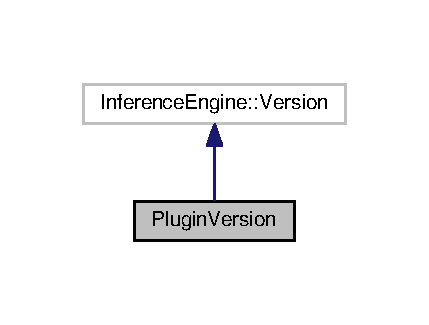
\includegraphics[width=206pt]{structPluginVersion__inherit__graph}
\end{center}
\end{figure}


Collaboration diagram for Plugin\+Version\+:
\nopagebreak
\begin{figure}[H]
\begin{center}
\leavevmode
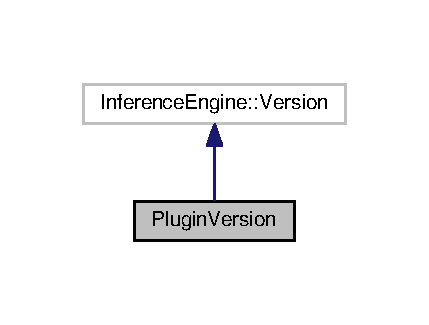
\includegraphics[width=206pt]{structPluginVersion__coll__graph}
\end{center}
\end{figure}
\subsection*{Public Member Functions}
\begin{DoxyCompactItemize}
\item 
\hyperlink{structPluginVersion_a1c1350a01e77363446153a0ecfccf1f9}{Plugin\+Version} (const Inference\+Engine\+::\+Version $\ast$ver)
\item 
\hyperlink{structPluginVersion_a9dd75e7684175bd4a0cd47181292d052}{operator bool} () const noexcept
\end{DoxyCompactItemize}
\subsection*{Public Attributes}
\begin{DoxyCompactItemize}
\item 
bool \hyperlink{structPluginVersion_a7c1d1b7b0b110266d67de10e3c909f29}{initialized} = false
\end{DoxyCompactItemize}


\subsection{Detailed Description}
A \hyperlink{structPluginVersion}{Plugin\+Version} class stores plugin version and initialization status. 

Definition at line 150 of file common.\+hpp.



\subsection{Constructor \& Destructor Documentation}
\index{Plugin\+Version@{Plugin\+Version}!Plugin\+Version@{Plugin\+Version}}
\index{Plugin\+Version@{Plugin\+Version}!Plugin\+Version@{Plugin\+Version}}
\subsubsection[{\texorpdfstring{Plugin\+Version(const Inference\+Engine\+::\+Version $\ast$ver)}{PluginVersion(const InferenceEngine::Version *ver)}}]{\setlength{\rightskip}{0pt plus 5cm}Plugin\+Version\+::\+Plugin\+Version (
\begin{DoxyParamCaption}
\item[{const Inference\+Engine\+::\+Version $\ast$}]{ver}
\end{DoxyParamCaption}
)\hspace{0.3cm}{\ttfamily [inline]}, {\ttfamily [explicit]}}\hypertarget{structPluginVersion_a1c1350a01e77363446153a0ecfccf1f9}{}\label{structPluginVersion_a1c1350a01e77363446153a0ecfccf1f9}


Definition at line 153 of file common.\+hpp.


\begin{DoxyCode}
153                                                               \{
154         \textcolor{keywordflow}{if} (\textcolor{keyword}{nullptr} == ver) \{
155             \textcolor{keywordflow}{return};
156         \}
157         InferenceEngine::Version::operator=(*ver);
158         \hyperlink{structPluginVersion_a7c1d1b7b0b110266d67de10e3c909f29}{initialized} = \textcolor{keyword}{true};
159     \}
\end{DoxyCode}


\subsection{Member Function Documentation}
\index{Plugin\+Version@{Plugin\+Version}!operator bool@{operator bool}}
\index{operator bool@{operator bool}!Plugin\+Version@{Plugin\+Version}}
\subsubsection[{\texorpdfstring{operator bool() const noexcept}{operator bool() const noexcept}}]{\setlength{\rightskip}{0pt plus 5cm}Plugin\+Version\+::operator bool (
\begin{DoxyParamCaption}
{}
\end{DoxyParamCaption}
) const\hspace{0.3cm}{\ttfamily [inline]}, {\ttfamily [noexcept]}}\hypertarget{structPluginVersion_a9dd75e7684175bd4a0cd47181292d052}{}\label{structPluginVersion_a9dd75e7684175bd4a0cd47181292d052}


Definition at line 161 of file common.\+hpp.


\begin{DoxyCode}
161                                    \{
162         \textcolor{keywordflow}{return} \hyperlink{structPluginVersion_a7c1d1b7b0b110266d67de10e3c909f29}{initialized};
163     \}
\end{DoxyCode}


\subsection{Member Data Documentation}
\index{Plugin\+Version@{Plugin\+Version}!initialized@{initialized}}
\index{initialized@{initialized}!Plugin\+Version@{Plugin\+Version}}
\subsubsection[{\texorpdfstring{initialized}{initialized}}]{\setlength{\rightskip}{0pt plus 5cm}bool Plugin\+Version\+::initialized = false}\hypertarget{structPluginVersion_a7c1d1b7b0b110266d67de10e3c909f29}{}\label{structPluginVersion_a7c1d1b7b0b110266d67de10e3c909f29}


Definition at line 151 of file common.\+hpp.



The documentation for this class was generated from the following file\+:\begin{DoxyCompactItemize}
\item 
include/openvino\+\_\+service/\hyperlink{common_8hpp}{common.\+hpp}\end{DoxyCompactItemize}

\hypertarget{classInferenceEngine_1_1Extensions_1_1Cpu_1_1PowerFileImpl}{}\section{Inference\+Engine\+:\+:Extensions\+:\+:Cpu\+:\+:Power\+File\+Impl Class Reference}
\label{classInferenceEngine_1_1Extensions_1_1Cpu_1_1PowerFileImpl}\index{Inference\+Engine\+::\+Extensions\+::\+Cpu\+::\+Power\+File\+Impl@{Inference\+Engine\+::\+Extensions\+::\+Cpu\+::\+Power\+File\+Impl}}


Inheritance diagram for Inference\+Engine\+:\+:Extensions\+:\+:Cpu\+:\+:Power\+File\+Impl\+:
\nopagebreak
\begin{figure}[H]
\begin{center}
\leavevmode
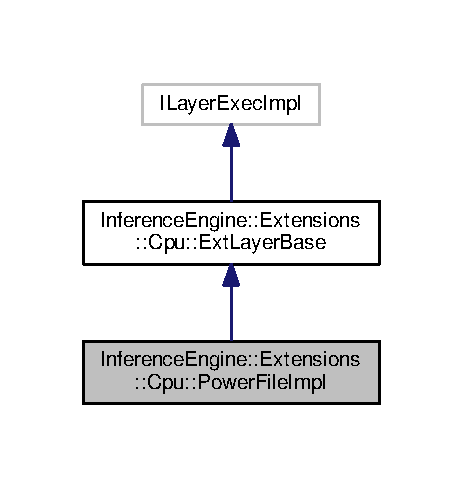
\includegraphics[width=222pt]{classInferenceEngine_1_1Extensions_1_1Cpu_1_1PowerFileImpl__inherit__graph}
\end{center}
\end{figure}


Collaboration diagram for Inference\+Engine\+:\+:Extensions\+:\+:Cpu\+:\+:Power\+File\+Impl\+:
\nopagebreak
\begin{figure}[H]
\begin{center}
\leavevmode
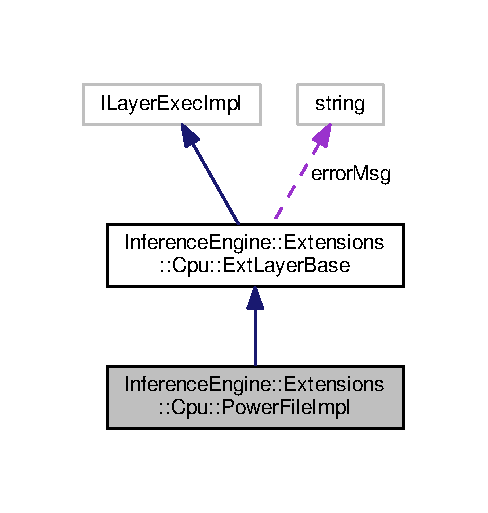
\includegraphics[width=234pt]{classInferenceEngine_1_1Extensions_1_1Cpu_1_1PowerFileImpl__coll__graph}
\end{center}
\end{figure}
\subsection*{Public Member Functions}
\begin{DoxyCompactItemize}
\item 
\hyperlink{classInferenceEngine_1_1Extensions_1_1Cpu_1_1PowerFileImpl_ac76ea1f22e816a9338136184f5a83a93}{Power\+File\+Impl} (const C\+N\+N\+Layer $\ast$layer)
\item 
Status\+Code \hyperlink{classInferenceEngine_1_1Extensions_1_1Cpu_1_1PowerFileImpl_a21992abbdf72f126effab37b24d724b1}{execute} (std\+::vector$<$ Blob\+::\+Ptr $>$ \&inputs, std\+::vector$<$ Blob\+::\+Ptr $>$ \&outputs, Response\+Desc $\ast$resp) noexceptoverride
\end{DoxyCompactItemize}
\subsection*{Additional Inherited Members}


\subsection{Detailed Description}


Definition at line 28 of file ext\+\_\+powerfile.\+cpp.



\subsection{Constructor \& Destructor Documentation}
\index{Inference\+Engine\+::\+Extensions\+::\+Cpu\+::\+Power\+File\+Impl@{Inference\+Engine\+::\+Extensions\+::\+Cpu\+::\+Power\+File\+Impl}!Power\+File\+Impl@{Power\+File\+Impl}}
\index{Power\+File\+Impl@{Power\+File\+Impl}!Inference\+Engine\+::\+Extensions\+::\+Cpu\+::\+Power\+File\+Impl@{Inference\+Engine\+::\+Extensions\+::\+Cpu\+::\+Power\+File\+Impl}}
\subsubsection[{\texorpdfstring{Power\+File\+Impl(const C\+N\+N\+Layer $\ast$layer)}{PowerFileImpl(const CNNLayer *layer)}}]{\setlength{\rightskip}{0pt plus 5cm}Inference\+Engine\+::\+Extensions\+::\+Cpu\+::\+Power\+File\+Impl\+::\+Power\+File\+Impl (
\begin{DoxyParamCaption}
\item[{const C\+N\+N\+Layer $\ast$}]{layer}
\end{DoxyParamCaption}
)\hspace{0.3cm}{\ttfamily [inline]}, {\ttfamily [explicit]}}\hypertarget{classInferenceEngine_1_1Extensions_1_1Cpu_1_1PowerFileImpl_ac76ea1f22e816a9338136184f5a83a93}{}\label{classInferenceEngine_1_1Extensions_1_1Cpu_1_1PowerFileImpl_ac76ea1f22e816a9338136184f5a83a93}


Definition at line 30 of file ext\+\_\+powerfile.\+cpp.


\begin{DoxyCode}
30                                                  : \hyperlink{classInferenceEngine_1_1Extensions_1_1Cpu_1_1ExtLayerBase_affff0e8263ca26852ccf71d299d7b06a}{ExtLayerBase}(layer) \{
31         \textcolor{keywordflow}{try} \{
32             \textcolor{keywordflow}{if} (\hyperlink{classInferenceEngine_1_1Extensions_1_1Cpu_1_1ExtLayerBase_a1074cdccacb9e9ca6eec01bbc2f7ca4a}{cnnLayer}.insData.size() != 1 || \hyperlink{classInferenceEngine_1_1Extensions_1_1Cpu_1_1ExtLayerBase_a1074cdccacb9e9ca6eec01bbc2f7ca4a}{cnnLayer}.outData.empty())
33                 THROW\_IE\_EXCEPTION << \textcolor{stringliteral}{"Incorrect number of input/output edges!"};
34 
35             \textcolor{comment}{// TODO: load this from some file or as blob?}
36             shift\_.push\_back(1);
37             shift\_.push\_back(0);
38             shift\_.push\_back(0);
39             shift\_.push\_back(0);
40             shift\_.push\_back(1);
41             shift\_.push\_back(0);
42 
43             \hyperlink{classInferenceEngine_1_1Extensions_1_1Cpu_1_1ExtLayerBase_a0ac7a6632e95b9500d5246b05b4b0bfa}{addConfig}(\{DataConfigurator(\hyperlink{classInferenceEngine_1_1Extensions_1_1Cpu_1_1ExtLayerBase_a1258a8d209e0249e0b1717618352ddfba446687ea2db1ada75be5ed053be77f59}{ConfLayout::PLN})\}, \{DataConfigurator(
      \hyperlink{classInferenceEngine_1_1Extensions_1_1Cpu_1_1ExtLayerBase_a1258a8d209e0249e0b1717618352ddfba446687ea2db1ada75be5ed053be77f59}{ConfLayout::PLN})\});
44         \} \textcolor{keywordflow}{catch} (InferenceEngine::details::InferenceEngineException &ex) \{
45             \hyperlink{classInferenceEngine_1_1Extensions_1_1Cpu_1_1ExtLayerBase_abc78e9b5a79fa339ffd831a5318f71f7}{errorMsg} = ex.what();
46         \}
47     \}
\end{DoxyCode}


\subsection{Member Function Documentation}
\index{Inference\+Engine\+::\+Extensions\+::\+Cpu\+::\+Power\+File\+Impl@{Inference\+Engine\+::\+Extensions\+::\+Cpu\+::\+Power\+File\+Impl}!execute@{execute}}
\index{execute@{execute}!Inference\+Engine\+::\+Extensions\+::\+Cpu\+::\+Power\+File\+Impl@{Inference\+Engine\+::\+Extensions\+::\+Cpu\+::\+Power\+File\+Impl}}
\subsubsection[{\texorpdfstring{execute(std\+::vector$<$ Blob\+::\+Ptr $>$ \&inputs, std\+::vector$<$ Blob\+::\+Ptr $>$ \&outputs, Response\+Desc $\ast$resp) noexceptoverride}{execute(std::vector< Blob::Ptr > &inputs, std::vector< Blob::Ptr > &outputs, ResponseDesc *resp) noexceptoverride}}]{\setlength{\rightskip}{0pt plus 5cm}Status\+Code Inference\+Engine\+::\+Extensions\+::\+Cpu\+::\+Power\+File\+Impl\+::execute (
\begin{DoxyParamCaption}
\item[{std\+::vector$<$ Blob\+::\+Ptr $>$ \&}]{inputs, }
\item[{std\+::vector$<$ Blob\+::\+Ptr $>$ \&}]{outputs, }
\item[{Response\+Desc $\ast$}]{resp}
\end{DoxyParamCaption}
)\hspace{0.3cm}{\ttfamily [inline]}, {\ttfamily [override]}, {\ttfamily [noexcept]}}\hypertarget{classInferenceEngine_1_1Extensions_1_1Cpu_1_1PowerFileImpl_a21992abbdf72f126effab37b24d724b1}{}\label{classInferenceEngine_1_1Extensions_1_1Cpu_1_1PowerFileImpl_a21992abbdf72f126effab37b24d724b1}


Definition at line 49 of file ext\+\_\+powerfile.\+cpp.


\begin{DoxyCode}
50                                                              \{
51         \textcolor{keywordflow}{if} (inputs.size() != 1 || outputs.empty()) \{
52             \textcolor{keywordflow}{if} (resp) \{
53                 std::string \hyperlink{classInferenceEngine_1_1Extensions_1_1Cpu_1_1ExtLayerBase_abc78e9b5a79fa339ffd831a5318f71f7}{errorMsg} = \textcolor{stringliteral}{"Incorrect number of input or output edges!"};
54                 errorMsg.copy(resp->msg, \textcolor{keyword}{sizeof}(resp->msg) - 1);
55             \}
56             \textcolor{keywordflow}{return} GENERAL\_ERROR;
57         \}
58         \textcolor{keywordtype}{float}* src\_data = inputs[0]->buffer();
59         \textcolor{keywordtype}{float}* dst\_data = outputs[0]->buffer();
60 
61         \textcolor{keywordflow}{for} (\textcolor{keywordtype}{size\_t} i = 0; i < inputs[0]->size(); i++) \{
62             \textcolor{keywordtype}{size\_t} shift\_idx = i % shift\_.size();
63             dst\_data[i] = src\_data[i] + shift\_[shift\_idx];
64         \}
65         \textcolor{keywordflow}{return} OK;
66     \}
\end{DoxyCode}


The documentation for this class was generated from the following file\+:\begin{DoxyCompactItemize}
\item 
thirdparty/extension/\hyperlink{ext__powerfile_8cpp}{ext\+\_\+powerfile.\+cpp}\end{DoxyCompactItemize}

\hypertarget{classInferenceEngine_1_1Extensions_1_1Cpu_1_1PriorBoxClusteredImpl}{}\section{Inference\+Engine\+:\+:Extensions\+:\+:Cpu\+:\+:Prior\+Box\+Clustered\+Impl Class Reference}
\label{classInferenceEngine_1_1Extensions_1_1Cpu_1_1PriorBoxClusteredImpl}\index{Inference\+Engine\+::\+Extensions\+::\+Cpu\+::\+Prior\+Box\+Clustered\+Impl@{Inference\+Engine\+::\+Extensions\+::\+Cpu\+::\+Prior\+Box\+Clustered\+Impl}}


Inheritance diagram for Inference\+Engine\+:\+:Extensions\+:\+:Cpu\+:\+:Prior\+Box\+Clustered\+Impl\+:
\nopagebreak
\begin{figure}[H]
\begin{center}
\leavevmode
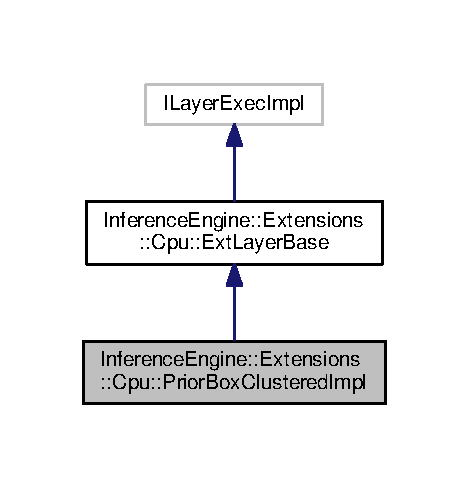
\includegraphics[width=225pt]{classInferenceEngine_1_1Extensions_1_1Cpu_1_1PriorBoxClusteredImpl__inherit__graph}
\end{center}
\end{figure}


Collaboration diagram for Inference\+Engine\+:\+:Extensions\+:\+:Cpu\+:\+:Prior\+Box\+Clustered\+Impl\+:
\nopagebreak
\begin{figure}[H]
\begin{center}
\leavevmode
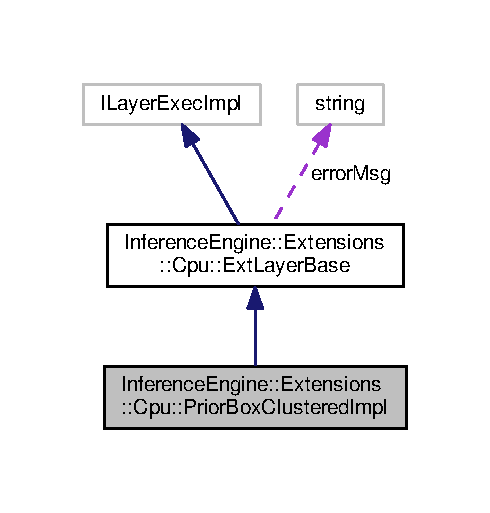
\includegraphics[width=235pt]{classInferenceEngine_1_1Extensions_1_1Cpu_1_1PriorBoxClusteredImpl__coll__graph}
\end{center}
\end{figure}
\subsection*{Public Member Functions}
\begin{DoxyCompactItemize}
\item 
\hyperlink{classInferenceEngine_1_1Extensions_1_1Cpu_1_1PriorBoxClusteredImpl_aa226e0233fc9287bded34c700f0e5073}{Prior\+Box\+Clustered\+Impl} (const C\+N\+N\+Layer $\ast$layer)
\item 
Status\+Code \hyperlink{classInferenceEngine_1_1Extensions_1_1Cpu_1_1PriorBoxClusteredImpl_ab0731b9592c833201a2df75282b9aea1}{execute} (std\+::vector$<$ Blob\+::\+Ptr $>$ \&inputs, std\+::vector$<$ Blob\+::\+Ptr $>$ \&outputs, Response\+Desc $\ast$resp) noexceptoverride
\end{DoxyCompactItemize}
\subsection*{Additional Inherited Members}


\subsection{Detailed Description}


Definition at line 26 of file ext\+\_\+priorbox\+\_\+clustered.\+cpp.



\subsection{Constructor \& Destructor Documentation}
\index{Inference\+Engine\+::\+Extensions\+::\+Cpu\+::\+Prior\+Box\+Clustered\+Impl@{Inference\+Engine\+::\+Extensions\+::\+Cpu\+::\+Prior\+Box\+Clustered\+Impl}!Prior\+Box\+Clustered\+Impl@{Prior\+Box\+Clustered\+Impl}}
\index{Prior\+Box\+Clustered\+Impl@{Prior\+Box\+Clustered\+Impl}!Inference\+Engine\+::\+Extensions\+::\+Cpu\+::\+Prior\+Box\+Clustered\+Impl@{Inference\+Engine\+::\+Extensions\+::\+Cpu\+::\+Prior\+Box\+Clustered\+Impl}}
\subsubsection[{\texorpdfstring{Prior\+Box\+Clustered\+Impl(const C\+N\+N\+Layer $\ast$layer)}{PriorBoxClusteredImpl(const CNNLayer *layer)}}]{\setlength{\rightskip}{0pt plus 5cm}Inference\+Engine\+::\+Extensions\+::\+Cpu\+::\+Prior\+Box\+Clustered\+Impl\+::\+Prior\+Box\+Clustered\+Impl (
\begin{DoxyParamCaption}
\item[{const C\+N\+N\+Layer $\ast$}]{layer}
\end{DoxyParamCaption}
)\hspace{0.3cm}{\ttfamily [inline]}, {\ttfamily [explicit]}}\hypertarget{classInferenceEngine_1_1Extensions_1_1Cpu_1_1PriorBoxClusteredImpl_aa226e0233fc9287bded34c700f0e5073}{}\label{classInferenceEngine_1_1Extensions_1_1Cpu_1_1PriorBoxClusteredImpl_aa226e0233fc9287bded34c700f0e5073}


Definition at line 28 of file ext\+\_\+priorbox\+\_\+clustered.\+cpp.


\begin{DoxyCode}
28                                                          : \hyperlink{classInferenceEngine_1_1Extensions_1_1Cpu_1_1ExtLayerBase_affff0e8263ca26852ccf71d299d7b06a}{ExtLayerBase}(layer) \{
29         \textcolor{keywordflow}{try} \{
30             \textcolor{keywordflow}{if} (\hyperlink{classInferenceEngine_1_1Extensions_1_1Cpu_1_1ExtLayerBase_a1074cdccacb9e9ca6eec01bbc2f7ca4a}{cnnLayer}.insData.size() != 2 || \hyperlink{classInferenceEngine_1_1Extensions_1_1Cpu_1_1ExtLayerBase_a1074cdccacb9e9ca6eec01bbc2f7ca4a}{cnnLayer}.outData.empty())
31                 THROW\_IE\_EXCEPTION << \textcolor{stringliteral}{"Incorrect number of input/output edges!"};
32 
33             widths\_ = \hyperlink{classInferenceEngine_1_1Extensions_1_1Cpu_1_1ExtLayerBase_a1074cdccacb9e9ca6eec01bbc2f7ca4a}{cnnLayer}.GetParamAsFloats(\textcolor{stringliteral}{"width"}, \{\});
34             heights\_ = \hyperlink{classInferenceEngine_1_1Extensions_1_1Cpu_1_1ExtLayerBase_a1074cdccacb9e9ca6eec01bbc2f7ca4a}{cnnLayer}.GetParamAsFloats(\textcolor{stringliteral}{"height"}, \{\});
35             clip\_ = \hyperlink{classInferenceEngine_1_1Extensions_1_1Cpu_1_1ExtLayerBase_a1074cdccacb9e9ca6eec01bbc2f7ca4a}{cnnLayer}.GetParamAsInt(\textcolor{stringliteral}{"clip"});
36             variance\_ = \hyperlink{classInferenceEngine_1_1Extensions_1_1Cpu_1_1ExtLayerBase_a1074cdccacb9e9ca6eec01bbc2f7ca4a}{cnnLayer}.GetParamAsFloats(\textcolor{stringliteral}{"variance"}, \{\});
37             img\_h\_ = \hyperlink{classInferenceEngine_1_1Extensions_1_1Cpu_1_1ExtLayerBase_a1074cdccacb9e9ca6eec01bbc2f7ca4a}{cnnLayer}.GetParamAsInt(\textcolor{stringliteral}{"img\_h"}, 0);
38             img\_w\_ = \hyperlink{classInferenceEngine_1_1Extensions_1_1Cpu_1_1ExtLayerBase_a1074cdccacb9e9ca6eec01bbc2f7ca4a}{cnnLayer}.GetParamAsInt(\textcolor{stringliteral}{"img\_w"}, 0);
39             step\_ = \hyperlink{classInferenceEngine_1_1Extensions_1_1Cpu_1_1ExtLayerBase_a1074cdccacb9e9ca6eec01bbc2f7ca4a}{cnnLayer}.GetParamAsFloat(\textcolor{stringliteral}{"step"}, 0);
40             step\_h\_ = \hyperlink{classInferenceEngine_1_1Extensions_1_1Cpu_1_1ExtLayerBase_a1074cdccacb9e9ca6eec01bbc2f7ca4a}{cnnLayer}.GetParamAsFloat(\textcolor{stringliteral}{"step\_h"}, 0);
41             step\_w\_ = \hyperlink{classInferenceEngine_1_1Extensions_1_1Cpu_1_1ExtLayerBase_a1074cdccacb9e9ca6eec01bbc2f7ca4a}{cnnLayer}.GetParamAsFloat(\textcolor{stringliteral}{"step\_w"}, 0);
42             offset\_ = \hyperlink{classInferenceEngine_1_1Extensions_1_1Cpu_1_1ExtLayerBase_a1074cdccacb9e9ca6eec01bbc2f7ca4a}{cnnLayer}.GetParamAsFloat(\textcolor{stringliteral}{"offset"});
43 
44             \hyperlink{classInferenceEngine_1_1Extensions_1_1Cpu_1_1ExtLayerBase_a0ac7a6632e95b9500d5246b05b4b0bfa}{addConfig}(\{\{\hyperlink{classInferenceEngine_1_1Extensions_1_1Cpu_1_1ExtLayerBase_a1258a8d209e0249e0b1717618352ddfba446687ea2db1ada75be5ed053be77f59}{ConfLayout::PLN}, \textcolor{keyword}{true}\}, \{
      \hyperlink{classInferenceEngine_1_1Extensions_1_1Cpu_1_1ExtLayerBase_a1258a8d209e0249e0b1717618352ddfba446687ea2db1ada75be5ed053be77f59}{ConfLayout::PLN}, \textcolor{keyword}{true}\}\}, \{\{\hyperlink{classInferenceEngine_1_1Extensions_1_1Cpu_1_1ExtLayerBase_a1258a8d209e0249e0b1717618352ddfba446687ea2db1ada75be5ed053be77f59}{ConfLayout::PLN}, \textcolor{keyword}{true}\}\});
45         \} \textcolor{keywordflow}{catch} (InferenceEngine::details::InferenceEngineException &ex) \{
46             \hyperlink{classInferenceEngine_1_1Extensions_1_1Cpu_1_1ExtLayerBase_abc78e9b5a79fa339ffd831a5318f71f7}{errorMsg} = ex.what();
47         \}
48     \}
\end{DoxyCode}


\subsection{Member Function Documentation}
\index{Inference\+Engine\+::\+Extensions\+::\+Cpu\+::\+Prior\+Box\+Clustered\+Impl@{Inference\+Engine\+::\+Extensions\+::\+Cpu\+::\+Prior\+Box\+Clustered\+Impl}!execute@{execute}}
\index{execute@{execute}!Inference\+Engine\+::\+Extensions\+::\+Cpu\+::\+Prior\+Box\+Clustered\+Impl@{Inference\+Engine\+::\+Extensions\+::\+Cpu\+::\+Prior\+Box\+Clustered\+Impl}}
\subsubsection[{\texorpdfstring{execute(std\+::vector$<$ Blob\+::\+Ptr $>$ \&inputs, std\+::vector$<$ Blob\+::\+Ptr $>$ \&outputs, Response\+Desc $\ast$resp) noexceptoverride}{execute(std::vector< Blob::Ptr > &inputs, std::vector< Blob::Ptr > &outputs, ResponseDesc *resp) noexceptoverride}}]{\setlength{\rightskip}{0pt plus 5cm}Status\+Code Inference\+Engine\+::\+Extensions\+::\+Cpu\+::\+Prior\+Box\+Clustered\+Impl\+::execute (
\begin{DoxyParamCaption}
\item[{std\+::vector$<$ Blob\+::\+Ptr $>$ \&}]{inputs, }
\item[{std\+::vector$<$ Blob\+::\+Ptr $>$ \&}]{outputs, }
\item[{Response\+Desc $\ast$}]{resp}
\end{DoxyParamCaption}
)\hspace{0.3cm}{\ttfamily [inline]}, {\ttfamily [override]}, {\ttfamily [noexcept]}}\hypertarget{classInferenceEngine_1_1Extensions_1_1Cpu_1_1PriorBoxClusteredImpl_ab0731b9592c833201a2df75282b9aea1}{}\label{classInferenceEngine_1_1Extensions_1_1Cpu_1_1PriorBoxClusteredImpl_ab0731b9592c833201a2df75282b9aea1}


Definition at line 50 of file ext\+\_\+priorbox\+\_\+clustered.\+cpp.


\begin{DoxyCode}
51                                                              \{
52         \textcolor{keywordtype}{int} num\_priors\_ = widths\_.size();
53 
54         \textcolor{keywordflow}{if} (variance\_.empty())
55             variance\_.push\_back(0.1);
56 
57         \textcolor{comment}{// Execute}
58         \textcolor{keyword}{const} \textcolor{keywordtype}{int} layer\_width = inputs[0]->getTensorDesc().getDims()[3];
59         \textcolor{keyword}{const} \textcolor{keywordtype}{int} layer\_height = inputs[0]->getTensorDesc().getDims()[2];
60 
61         \textcolor{keywordtype}{int} img\_width = img\_w\_ == 0 ? inputs[1]->getTensorDesc().getDims()[3] : img\_w\_;
62         \textcolor{keywordtype}{int} img\_height = img\_h\_ == 0 ? inputs[1]->getTensorDesc().getDims()[2] : img\_h\_;
63 
64         \textcolor{keywordtype}{float} step\_w = step\_w\_ == 0 ? step\_ : step\_w\_;
65         \textcolor{keywordtype}{float} step\_h = step\_h\_ == 0 ? step\_ : step\_h\_;
66 
67         \textcolor{keyword}{auto} *top\_data\_0 = outputs[0]->buffer().as<\textcolor{keywordtype}{float} *>();
68         \textcolor{keywordtype}{float} *top\_data\_1 = top\_data\_0 + outputs[0]->getTensorDesc().getDims()[2];
69         \textcolor{keywordtype}{int} var\_size = variance\_.size();
70 
71         \textcolor{keywordflow}{for} (\textcolor{keywordtype}{int} h = 0; h < layer\_height; ++h) \{
72             \textcolor{keywordflow}{for} (\textcolor{keywordtype}{int} w = 0; w < layer\_width; ++w) \{
73                 \textcolor{keywordtype}{float} center\_x = (w + offset\_) * step\_w;
74                 \textcolor{keywordtype}{float} center\_y = (h + offset\_) * step\_h;
75 
76                 \textcolor{keywordflow}{for} (\textcolor{keywordtype}{int} s = 0; s < num\_priors\_; ++s) \{
77                     \textcolor{keywordtype}{float} box\_width = widths\_[s];
78                     \textcolor{keywordtype}{float} box\_height = heights\_[s];
79 
80                     \textcolor{keywordtype}{float} xmin = (center\_x - box\_width / 2.) / img\_width;
81                     \textcolor{keywordtype}{float} ymin = (center\_y - box\_height / 2.) / img\_height;
82                     \textcolor{keywordtype}{float} xmax = (center\_x + box\_width / 2.) / img\_width;
83                     \textcolor{keywordtype}{float} ymax = (center\_y + box\_height / 2.) / img\_height;
84 
85                     \textcolor{keywordflow}{if} (clip\_) \{
86                         xmin = std::min(std::max(xmin, 0.0f), 1.0f);
87                         ymin = std::min(std::max(ymin, 0.0f), 1.0f);
88                         xmax = std::min(std::max(xmax, 0.0f), 1.0f);
89                         ymax = std::min(std::max(ymax, 0.0f), 1.0f);
90                     \}
91 
92                     top\_data\_0[h * layer\_width * num\_priors\_ * 4 + w * num\_priors\_ * 4 + s * 4 + 0] = xmin;
93                     top\_data\_0[h * layer\_width * num\_priors\_ * 4 + w * num\_priors\_ * 4 + s * 4 + 1] = ymin;
94                     top\_data\_0[h * layer\_width * num\_priors\_ * 4 + w * num\_priors\_ * 4 + s * 4 + 2] = xmax;
95                     top\_data\_0[h * layer\_width * num\_priors\_ * 4 + w * num\_priors\_ * 4 + s * 4 + 3] = ymax;
96 
97                     \textcolor{keywordflow}{for} (\textcolor{keywordtype}{int} j = 0; j < var\_size; j++)
98                         top\_data\_1[h * layer\_width * num\_priors\_ * var\_size + w * num\_priors\_ * var\_size +
99                                    s * var\_size +
100                                    j] = variance\_[j];
101                 \}
102             \}
103         \}
104         \textcolor{keywordflow}{return} OK;
105     \}
\end{DoxyCode}


The documentation for this class was generated from the following file\+:\begin{DoxyCompactItemize}
\item 
thirdparty/extension/\hyperlink{ext__priorbox__clustered_8cpp}{ext\+\_\+priorbox\+\_\+clustered.\+cpp}\end{DoxyCompactItemize}

\hypertarget{classInferenceEngine_1_1Extensions_1_1Cpu_1_1PriorBoxImpl}{}\section{Inference\+Engine\+:\+:Extensions\+:\+:Cpu\+:\+:Prior\+Box\+Impl Class Reference}
\label{classInferenceEngine_1_1Extensions_1_1Cpu_1_1PriorBoxImpl}\index{Inference\+Engine\+::\+Extensions\+::\+Cpu\+::\+Prior\+Box\+Impl@{Inference\+Engine\+::\+Extensions\+::\+Cpu\+::\+Prior\+Box\+Impl}}


Inheritance diagram for Inference\+Engine\+:\+:Extensions\+:\+:Cpu\+:\+:Prior\+Box\+Impl\+:
\nopagebreak
\begin{figure}[H]
\begin{center}
\leavevmode
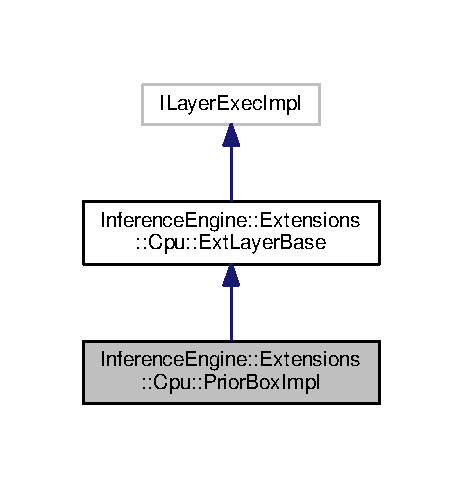
\includegraphics[width=222pt]{classInferenceEngine_1_1Extensions_1_1Cpu_1_1PriorBoxImpl__inherit__graph}
\end{center}
\end{figure}


Collaboration diagram for Inference\+Engine\+:\+:Extensions\+:\+:Cpu\+:\+:Prior\+Box\+Impl\+:
\nopagebreak
\begin{figure}[H]
\begin{center}
\leavevmode
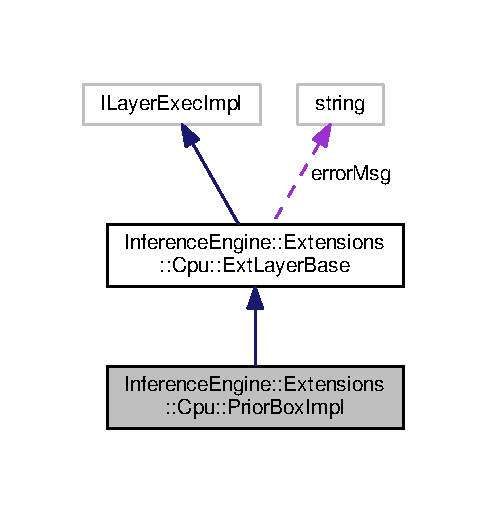
\includegraphics[width=234pt]{classInferenceEngine_1_1Extensions_1_1Cpu_1_1PriorBoxImpl__coll__graph}
\end{center}
\end{figure}
\subsection*{Public Member Functions}
\begin{DoxyCompactItemize}
\item 
\hyperlink{classInferenceEngine_1_1Extensions_1_1Cpu_1_1PriorBoxImpl_a20be25ea0e66288956fe988dcf9a57a2}{Prior\+Box\+Impl} (const C\+N\+N\+Layer $\ast$layer)
\item 
Status\+Code \hyperlink{classInferenceEngine_1_1Extensions_1_1Cpu_1_1PriorBoxImpl_a24ca1d655fb4044338dc19c41eb0a6fa}{execute} (std\+::vector$<$ Blob\+::\+Ptr $>$ \&inputs, std\+::vector$<$ Blob\+::\+Ptr $>$ \&outputs, Response\+Desc $\ast$resp) noexceptoverride
\end{DoxyCompactItemize}
\subsection*{Additional Inherited Members}


\subsection{Detailed Description}


Definition at line 28 of file ext\+\_\+priorbox.\+cpp.



\subsection{Constructor \& Destructor Documentation}
\index{Inference\+Engine\+::\+Extensions\+::\+Cpu\+::\+Prior\+Box\+Impl@{Inference\+Engine\+::\+Extensions\+::\+Cpu\+::\+Prior\+Box\+Impl}!Prior\+Box\+Impl@{Prior\+Box\+Impl}}
\index{Prior\+Box\+Impl@{Prior\+Box\+Impl}!Inference\+Engine\+::\+Extensions\+::\+Cpu\+::\+Prior\+Box\+Impl@{Inference\+Engine\+::\+Extensions\+::\+Cpu\+::\+Prior\+Box\+Impl}}
\subsubsection[{\texorpdfstring{Prior\+Box\+Impl(const C\+N\+N\+Layer $\ast$layer)}{PriorBoxImpl(const CNNLayer *layer)}}]{\setlength{\rightskip}{0pt plus 5cm}Inference\+Engine\+::\+Extensions\+::\+Cpu\+::\+Prior\+Box\+Impl\+::\+Prior\+Box\+Impl (
\begin{DoxyParamCaption}
\item[{const C\+N\+N\+Layer $\ast$}]{layer}
\end{DoxyParamCaption}
)\hspace{0.3cm}{\ttfamily [inline]}, {\ttfamily [explicit]}}\hypertarget{classInferenceEngine_1_1Extensions_1_1Cpu_1_1PriorBoxImpl_a20be25ea0e66288956fe988dcf9a57a2}{}\label{classInferenceEngine_1_1Extensions_1_1Cpu_1_1PriorBoxImpl_a20be25ea0e66288956fe988dcf9a57a2}


Definition at line 30 of file ext\+\_\+priorbox.\+cpp.


\begin{DoxyCode}
30                                                 : \hyperlink{classInferenceEngine_1_1Extensions_1_1Cpu_1_1ExtLayerBase_affff0e8263ca26852ccf71d299d7b06a}{ExtLayerBase}(layer) \{
31         \textcolor{keywordflow}{try} \{
32             \textcolor{keywordflow}{if} (\hyperlink{classInferenceEngine_1_1Extensions_1_1Cpu_1_1ExtLayerBase_a1074cdccacb9e9ca6eec01bbc2f7ca4a}{cnnLayer}.insData.size() != 2 || \hyperlink{classInferenceEngine_1_1Extensions_1_1Cpu_1_1ExtLayerBase_a1074cdccacb9e9ca6eec01bbc2f7ca4a}{cnnLayer}.outData.empty())
33                 THROW\_IE\_EXCEPTION << \textcolor{stringliteral}{"Incorrect number of input/output edges!"};
34             \_offset = \hyperlink{classInferenceEngine_1_1Extensions_1_1Cpu_1_1ExtLayerBase_a1074cdccacb9e9ca6eec01bbc2f7ca4a}{cnnLayer}.GetParamAsFloat(\textcolor{stringliteral}{"offset"});
35             \_step = \hyperlink{classInferenceEngine_1_1Extensions_1_1Cpu_1_1ExtLayerBase_a1074cdccacb9e9ca6eec01bbc2f7ca4a}{cnnLayer}.GetParamAsFloat(\textcolor{stringliteral}{"step"}, 0);
36             \_min\_sizes = \hyperlink{classInferenceEngine_1_1Extensions_1_1Cpu_1_1ExtLayerBase_a1074cdccacb9e9ca6eec01bbc2f7ca4a}{cnnLayer}.GetParamAsFloats(\textcolor{stringliteral}{"min\_size"}, \{\});
37             \_max\_sizes = \hyperlink{classInferenceEngine_1_1Extensions_1_1Cpu_1_1ExtLayerBase_a1074cdccacb9e9ca6eec01bbc2f7ca4a}{cnnLayer}.GetParamAsFloats(\textcolor{stringliteral}{"max\_size"}, \{\});
38             \_flip = \textcolor{keyword}{static\_cast<}\textcolor{keywordtype}{bool}\textcolor{keyword}{>}(\hyperlink{classInferenceEngine_1_1Extensions_1_1Cpu_1_1ExtLayerBase_a1074cdccacb9e9ca6eec01bbc2f7ca4a}{cnnLayer}.GetParamAsInt(\textcolor{stringliteral}{"flip"}));
39             \_clip = \textcolor{keyword}{static\_cast<}\textcolor{keywordtype}{bool}\textcolor{keyword}{>}(\hyperlink{classInferenceEngine_1_1Extensions_1_1Cpu_1_1ExtLayerBase_a1074cdccacb9e9ca6eec01bbc2f7ca4a}{cnnLayer}.GetParamAsInt(\textcolor{stringliteral}{"clip"}));
40             \_scale\_all\_sizes = \textcolor{keyword}{static\_cast<}\textcolor{keywordtype}{bool}\textcolor{keyword}{>}(\hyperlink{classInferenceEngine_1_1Extensions_1_1Cpu_1_1ExtLayerBase_a1074cdccacb9e9ca6eec01bbc2f7ca4a}{cnnLayer}.GetParamAsInt(\textcolor{stringliteral}{"scale\_all\_sizes"}, 1));
41 
42             \textcolor{keywordtype}{bool} exist;
43 
44             \_aspect\_ratios.push\_back(1.0f);
45 
46             \textcolor{keyword}{const} std::vector<float> aspect\_ratios = \hyperlink{classInferenceEngine_1_1Extensions_1_1Cpu_1_1ExtLayerBase_a1074cdccacb9e9ca6eec01bbc2f7ca4a}{cnnLayer}.GetParamAsFloats(\textcolor{stringliteral}{"aspect\_ratio"}, \{\});
47 
48             \textcolor{keywordflow}{for} (\textcolor{keywordtype}{float} aspect\_ratio : aspect\_ratios) \{
49                 exist = \textcolor{keyword}{false};
50 
51                 \textcolor{keywordflow}{for} (\textcolor{keywordtype}{float} \_aspect\_ratio : \_aspect\_ratios) \{
52                     \textcolor{keywordflow}{if} (fabs(aspect\_ratio - \_aspect\_ratio) < 1e-6) \{
53                         exist = \textcolor{keyword}{true};
54                         \textcolor{keywordflow}{break};
55                     \}
56                 \}
57 
58                 \textcolor{keywordflow}{if} (exist) \{
59                     \textcolor{keywordflow}{continue};
60                 \}
61 
62                 \_aspect\_ratios.push\_back(aspect\_ratio);
63 
64                 \textcolor{keywordflow}{if} (\_flip) \{
65                     \_aspect\_ratios.push\_back(1.0f / aspect\_ratio);
66                 \}
67             \}
68 
69             \textcolor{keywordflow}{if} (\_scale\_all\_sizes) \{
70                 \_num\_priors = \textcolor{keyword}{static\_cast<}\textcolor{keywordtype}{int}\textcolor{keyword}{>}(\_aspect\_ratios.size() * \_min\_sizes.size());
71             \} \textcolor{keywordflow}{else} \{
72                 \_num\_priors = \textcolor{keyword}{static\_cast<}\textcolor{keywordtype}{int}\textcolor{keyword}{>}(\_aspect\_ratios.size() + \_min\_sizes.size() - 1);
73             \}
74 
75             \textcolor{keywordflow}{for} (\textcolor{keyword}{auto} it = \_max\_sizes.begin(); it != \_max\_sizes.end(); it++) \{
76                 \_num\_priors += 1;
77             \}
78 
79             \textcolor{keyword}{const} std::vector<float> variance = \hyperlink{classInferenceEngine_1_1Extensions_1_1Cpu_1_1ExtLayerBase_a1074cdccacb9e9ca6eec01bbc2f7ca4a}{cnnLayer}.GetParamAsFloats(\textcolor{stringliteral}{"variance"}, \{\});
80 
81             \textcolor{keywordflow}{if} (variance.size() == 1 || variance.size() == 4) \{
82                 \textcolor{keywordflow}{for} (\textcolor{keywordtype}{float} i : variance) \{
83                     \textcolor{keywordflow}{if} (i < 0) \{
84                         THROW\_IE\_EXCEPTION << \textcolor{stringliteral}{"Variance must be > 0."};
85                     \}
86 
87                     \_variance.push\_back(i);
88                 \}
89             \} \textcolor{keywordflow}{else} \textcolor{keywordflow}{if} (variance.empty()) \{
90                 \_variance.push\_back(0.1f);
91             \} \textcolor{keywordflow}{else} \{
92                 THROW\_IE\_EXCEPTION << \textcolor{stringliteral}{"Wrong number of variance values. Not less than 1 and more than 4
       variance values."};
93             \}
94 
95             \hyperlink{classInferenceEngine_1_1Extensions_1_1Cpu_1_1ExtLayerBase_a0ac7a6632e95b9500d5246b05b4b0bfa}{addConfig}(\{\{\hyperlink{classInferenceEngine_1_1Extensions_1_1Cpu_1_1ExtLayerBase_a1258a8d209e0249e0b1717618352ddfba8e1bde3c3d303163521522cf1d62f21f}{ConfLayout::ANY}, \textcolor{keyword}{true}\}, \{
      \hyperlink{classInferenceEngine_1_1Extensions_1_1Cpu_1_1ExtLayerBase_a1258a8d209e0249e0b1717618352ddfba8e1bde3c3d303163521522cf1d62f21f}{ConfLayout::ANY}, \textcolor{keyword}{true}\}\}, \{\{\hyperlink{classInferenceEngine_1_1Extensions_1_1Cpu_1_1ExtLayerBase_a1258a8d209e0249e0b1717618352ddfba446687ea2db1ada75be5ed053be77f59}{ConfLayout::PLN}, \textcolor{keyword}{true}\}\});
96         \} \textcolor{keywordflow}{catch} (InferenceEngine::details::InferenceEngineException &ex) \{
97             \hyperlink{classInferenceEngine_1_1Extensions_1_1Cpu_1_1ExtLayerBase_abc78e9b5a79fa339ffd831a5318f71f7}{errorMsg} = ex.what();
98         \}
99     \}
\end{DoxyCode}


\subsection{Member Function Documentation}
\index{Inference\+Engine\+::\+Extensions\+::\+Cpu\+::\+Prior\+Box\+Impl@{Inference\+Engine\+::\+Extensions\+::\+Cpu\+::\+Prior\+Box\+Impl}!execute@{execute}}
\index{execute@{execute}!Inference\+Engine\+::\+Extensions\+::\+Cpu\+::\+Prior\+Box\+Impl@{Inference\+Engine\+::\+Extensions\+::\+Cpu\+::\+Prior\+Box\+Impl}}
\subsubsection[{\texorpdfstring{execute(std\+::vector$<$ Blob\+::\+Ptr $>$ \&inputs, std\+::vector$<$ Blob\+::\+Ptr $>$ \&outputs, Response\+Desc $\ast$resp) noexceptoverride}{execute(std::vector< Blob::Ptr > &inputs, std::vector< Blob::Ptr > &outputs, ResponseDesc *resp) noexceptoverride}}]{\setlength{\rightskip}{0pt plus 5cm}Status\+Code Inference\+Engine\+::\+Extensions\+::\+Cpu\+::\+Prior\+Box\+Impl\+::execute (
\begin{DoxyParamCaption}
\item[{std\+::vector$<$ Blob\+::\+Ptr $>$ \&}]{inputs, }
\item[{std\+::vector$<$ Blob\+::\+Ptr $>$ \&}]{outputs, }
\item[{Response\+Desc $\ast$}]{resp}
\end{DoxyParamCaption}
)\hspace{0.3cm}{\ttfamily [inline]}, {\ttfamily [override]}, {\ttfamily [noexcept]}}\hypertarget{classInferenceEngine_1_1Extensions_1_1Cpu_1_1PriorBoxImpl_a24ca1d655fb4044338dc19c41eb0a6fa}{}\label{classInferenceEngine_1_1Extensions_1_1Cpu_1_1PriorBoxImpl_a24ca1d655fb4044338dc19c41eb0a6fa}


Definition at line 101 of file ext\+\_\+priorbox.\+cpp.


\begin{DoxyCode}
102                                                              \{
103         \textcolor{keywordflow}{if} (inputs.size() != 2 || outputs.empty()) \{
104             \textcolor{keywordflow}{if} (resp) \{
105                 std::string \hyperlink{classInferenceEngine_1_1Extensions_1_1Cpu_1_1ExtLayerBase_abc78e9b5a79fa339ffd831a5318f71f7}{errorMsg} = \textcolor{stringliteral}{"Incorrect number of input or output edges!"};
106                 errorMsg.copy(resp->msg, \textcolor{keyword}{sizeof}(resp->msg) - 1);
107             \}
108             \textcolor{keywordflow}{return} GENERAL\_ERROR;
109         \}
110         \textcolor{keyword}{auto}& dataMemPtr = inputs[0];
111         \textcolor{keyword}{auto}& imageMemPtr = inputs[1];
112         \textcolor{keyword}{auto}& dstMemPtr = outputs[0];
113         SizeVector \_data\_dims = dataMemPtr->getTensorDesc().getDims();
114         SizeVector \_image\_dims = imageMemPtr->getTensorDesc().getDims();
115         \textcolor{keyword}{const} \textcolor{keywordtype}{int} W = \_data\_dims[3];
116         \textcolor{keyword}{const} \textcolor{keywordtype}{int} H = \_data\_dims[2];
117         \textcolor{keyword}{const} \textcolor{keywordtype}{int} IW = \_image\_dims[3];
118         \textcolor{keyword}{const} \textcolor{keywordtype}{int} IH = \_image\_dims[2];
119 
120         \textcolor{keyword}{const} \textcolor{keywordtype}{int} OH = dstMemPtr->getTensorDesc().getDims()[2];
121         \textcolor{keyword}{const} \textcolor{keywordtype}{int} OW = (dstMemPtr->getTensorDesc().getDims().size() == 3) ? 1 : dstMemPtr->getTensorDesc().
      getDims()[3];
122 
123         \textcolor{keywordtype}{float} step\_x = 0.0f;
124         \textcolor{keywordtype}{float} step\_y = 0.0f;
125 
126         \textcolor{keywordflow}{if} (\_step == 0) \{
127             step\_x = \textcolor{keyword}{static\_cast<}\textcolor{keywordtype}{float}\textcolor{keyword}{>}(IW) / W;
128             step\_y = \textcolor{keyword}{static\_cast<}\textcolor{keywordtype}{float}\textcolor{keyword}{>}(IH) / H;
129         \} \textcolor{keywordflow}{else} \{
130             step\_x = \_step;
131             step\_y = \_step;
132         \}
133 
134         \textcolor{keywordtype}{float}* dst\_data = dstMemPtr->buffer();
135 
136         \textcolor{keywordtype}{int} dim = H * W * \_num\_priors * 4;
137         \textcolor{keywordtype}{int} idx = 0;
138         \textcolor{keywordtype}{float} center\_x = 0.0f;
139         \textcolor{keywordtype}{float} center\_y = 0.0f;
140 
141         \textcolor{keywordtype}{float} box\_width;
142         \textcolor{keywordtype}{float} box\_height;
143 
144         \textcolor{keywordflow}{for} (\textcolor{keywordtype}{int} h = 0; h < H; ++h) \{
145             \textcolor{keywordflow}{for} (\textcolor{keywordtype}{int} w = 0; w < W; ++w) \{
146                 \textcolor{keywordflow}{for} (\textcolor{keywordtype}{size\_t} msIdx = 0; msIdx < \_min\_sizes.size(); msIdx++) \{
147                     \textcolor{keywordflow}{if} (\_step == 0) \{
148                         center\_x = (w + 0.5f) * step\_x;
149                         center\_y = (h + 0.5f) * step\_y;
150                     \} \textcolor{keywordflow}{else} \{
151                         center\_x = (\_offset + w) * \_step;
152                         center\_y = (\_offset + h) * \_step;
153                     \}
154 
155                     box\_width = \_min\_sizes[msIdx];
156                     box\_height = \_min\_sizes[msIdx];
157 
158                     dst\_data[idx++] = (center\_x - box\_width / 2.0f) / IW;
159                     dst\_data[idx++] = (center\_y - box\_height / 2.0f) / IH;
160                     dst\_data[idx++] = (center\_x + box\_width / 2.0f) / IW;
161                     dst\_data[idx++] = (center\_y + box\_height / 2.0f) / IH;
162 
163                     \textcolor{keywordflow}{if} (\_max\_sizes.size() > msIdx) \{
164                         box\_width = box\_height = sqrt(\_min\_sizes[msIdx] * \_max\_sizes[msIdx]);
165 
166                         dst\_data[idx++] = (center\_x - box\_width / 2.0f) / IW;
167                         dst\_data[idx++] = (center\_y - box\_height / 2.0f) / IH;
168                         dst\_data[idx++] = (center\_x + box\_width / 2.0f) / IW;
169                         dst\_data[idx++] = (center\_y + box\_height / 2.0f) / IH;
170                     \}
171 
172                     \textcolor{keywordflow}{if} (\_scale\_all\_sizes || (!\_scale\_all\_sizes && (msIdx == \_min\_sizes.size() - 1))) \{
173                         \textcolor{keywordtype}{size\_t} sIdx = \_scale\_all\_sizes ? msIdx : 0;
174                         \textcolor{keywordflow}{for} (\textcolor{keywordtype}{float} ar : \_aspect\_ratios) \{
175                             \textcolor{keywordflow}{if} (fabs(ar - 1.0f) < 1e-6) \{
176                                 \textcolor{keywordflow}{continue};
177                             \}
178 
179                             box\_width = \_min\_sizes[sIdx] * sqrt(ar);
180                             box\_height = \_min\_sizes[sIdx] / sqrt(ar);
181 
182                             dst\_data[idx++] = (center\_x - box\_width / 2.0f) / IW;
183                             dst\_data[idx++] = (center\_y - box\_height / 2.0f) / IH;
184                             dst\_data[idx++] = (center\_x + box\_width / 2.0f) / IW;
185                             dst\_data[idx++] = (center\_y + box\_height / 2.0f) / IH;
186                         \}
187                     \}
188                 \}
189             \}
190         \}
191 
192         \textcolor{keywordflow}{if} (\_clip) \{
193             \textcolor{keywordflow}{for} (\textcolor{keywordtype}{int} d = 0; d < dim; ++d) \{
194                 dst\_data[d] = (std::min)((std::max)(dst\_data[d], 0.0f), 1.0f);
195             \}
196         \}
197 
198         \textcolor{keywordtype}{int} channel\_size = OH * OW;
199 
200         dst\_data += channel\_size;
201 
202         \textcolor{keywordtype}{int} count = 0;
203         \textcolor{keywordflow}{if} (\_variance.size() == 1) \{
204             \textcolor{keywordflow}{for} (\textcolor{keywordtype}{int} i = 0; i < channel\_size; i++) \{
205                 dst\_data[i] = \_variance[0];
206             \}
207         \} \textcolor{keywordflow}{else} \{
208             \textcolor{keywordflow}{for} (\textcolor{keywordtype}{int} h = 0; h < H; ++h) \{
209                 \textcolor{keywordflow}{for} (\textcolor{keywordtype}{int} w = 0; w < W; ++w) \{
210                     \textcolor{keywordflow}{for} (\textcolor{keywordtype}{int} i = 0; i < \_num\_priors; ++i) \{
211                         \textcolor{keywordflow}{for} (\textcolor{keywordtype}{int} j = 0; j < 4; ++j) \{
212                             dst\_data[count] = \_variance[j];
213                             ++count;
214                         \}
215                     \}
216                 \}
217             \}
218         \}
219         \textcolor{keywordflow}{return} OK;
220     \}
\end{DoxyCode}


The documentation for this class was generated from the following file\+:\begin{DoxyCompactItemize}
\item 
thirdparty/extension/\hyperlink{ext__priorbox_8cpp}{ext\+\_\+priorbox.\+cpp}\end{DoxyCompactItemize}

\hypertarget{classInferenceEngine_1_1Extensions_1_1Cpu_1_1ProposalFactory}{}\section{Inference\+Engine\+:\+:Extensions\+:\+:Cpu\+:\+:Proposal\+Factory Class Reference}
\label{classInferenceEngine_1_1Extensions_1_1Cpu_1_1ProposalFactory}\index{Inference\+Engine\+::\+Extensions\+::\+Cpu\+::\+Proposal\+Factory@{Inference\+Engine\+::\+Extensions\+::\+Cpu\+::\+Proposal\+Factory}}


Inheritance diagram for Inference\+Engine\+:\+:Extensions\+:\+:Cpu\+:\+:Proposal\+Factory\+:
\nopagebreak
\begin{figure}[H]
\begin{center}
\leavevmode
\includegraphics[width=253pt]{classInferenceEngine_1_1Extensions_1_1Cpu_1_1ProposalFactory__inherit__graph}
\end{center}
\end{figure}


Collaboration diagram for Inference\+Engine\+:\+:Extensions\+:\+:Cpu\+:\+:Proposal\+Factory\+:
\nopagebreak
\begin{figure}[H]
\begin{center}
\leavevmode
\includegraphics[width=253pt]{classInferenceEngine_1_1Extensions_1_1Cpu_1_1ProposalFactory__coll__graph}
\end{center}
\end{figure}
\subsection*{Public Member Functions}
\begin{DoxyCompactItemize}
\item 
\hyperlink{classInferenceEngine_1_1Extensions_1_1Cpu_1_1ProposalFactory_a6a8e5f0081abbcf8db84d8e37337ce07}{Proposal\+Factory} (const C\+N\+N\+Layer $\ast$layer)
\item 
Status\+Code \hyperlink{classInferenceEngine_1_1Extensions_1_1Cpu_1_1ProposalFactory_af55cd62ce5ffe6d22b708fb00befca55}{get\+Shapes} (const std\+::vector$<$ Tensor\+Desc $>$ \&in\+Shapes, std\+::vector$<$ Tensor\+Desc $>$ \&out\+Shapes, Response\+Desc $\ast$resp) noexceptoverride
\end{DoxyCompactItemize}
\subsection*{Additional Inherited Members}


\subsection{Detailed Description}


Definition at line 497 of file ext\+\_\+proposal.\+cpp.



\subsection{Constructor \& Destructor Documentation}
\index{Inference\+Engine\+::\+Extensions\+::\+Cpu\+::\+Proposal\+Factory@{Inference\+Engine\+::\+Extensions\+::\+Cpu\+::\+Proposal\+Factory}!Proposal\+Factory@{Proposal\+Factory}}
\index{Proposal\+Factory@{Proposal\+Factory}!Inference\+Engine\+::\+Extensions\+::\+Cpu\+::\+Proposal\+Factory@{Inference\+Engine\+::\+Extensions\+::\+Cpu\+::\+Proposal\+Factory}}
\subsubsection[{\texorpdfstring{Proposal\+Factory(const C\+N\+N\+Layer $\ast$layer)}{ProposalFactory(const CNNLayer *layer)}}]{\setlength{\rightskip}{0pt plus 5cm}Inference\+Engine\+::\+Extensions\+::\+Cpu\+::\+Proposal\+Factory\+::\+Proposal\+Factory (
\begin{DoxyParamCaption}
\item[{const C\+N\+N\+Layer $\ast$}]{layer}
\end{DoxyParamCaption}
)\hspace{0.3cm}{\ttfamily [inline]}, {\ttfamily [explicit]}}\hypertarget{classInferenceEngine_1_1Extensions_1_1Cpu_1_1ProposalFactory_a6a8e5f0081abbcf8db84d8e37337ce07}{}\label{classInferenceEngine_1_1Extensions_1_1Cpu_1_1ProposalFactory_a6a8e5f0081abbcf8db84d8e37337ce07}


Definition at line 499 of file ext\+\_\+proposal.\+cpp.


\begin{DoxyCode}
499 : \hyperlink{classInferenceEngine_1_1Extensions_1_1Cpu_1_1ImplFactory_a86837f88ce5c196382c1f7c38e3ba3a8}{ImplFactory}(layer) \{\}
\end{DoxyCode}


\subsection{Member Function Documentation}
\index{Inference\+Engine\+::\+Extensions\+::\+Cpu\+::\+Proposal\+Factory@{Inference\+Engine\+::\+Extensions\+::\+Cpu\+::\+Proposal\+Factory}!get\+Shapes@{get\+Shapes}}
\index{get\+Shapes@{get\+Shapes}!Inference\+Engine\+::\+Extensions\+::\+Cpu\+::\+Proposal\+Factory@{Inference\+Engine\+::\+Extensions\+::\+Cpu\+::\+Proposal\+Factory}}
\subsubsection[{\texorpdfstring{get\+Shapes(const std\+::vector$<$ Tensor\+Desc $>$ \&in\+Shapes, std\+::vector$<$ Tensor\+Desc $>$ \&out\+Shapes, Response\+Desc $\ast$resp) noexceptoverride}{getShapes(const std::vector< TensorDesc > &inShapes, std::vector< TensorDesc > &outShapes, ResponseDesc *resp) noexceptoverride}}]{\setlength{\rightskip}{0pt plus 5cm}Status\+Code Inference\+Engine\+::\+Extensions\+::\+Cpu\+::\+Proposal\+Factory\+::get\+Shapes (
\begin{DoxyParamCaption}
\item[{const std\+::vector$<$ Tensor\+Desc $>$ \&}]{in\+Shapes, }
\item[{std\+::vector$<$ Tensor\+Desc $>$ \&}]{out\+Shapes, }
\item[{Response\+Desc $\ast$}]{resp}
\end{DoxyParamCaption}
)\hspace{0.3cm}{\ttfamily [inline]}, {\ttfamily [override]}, {\ttfamily [noexcept]}}\hypertarget{classInferenceEngine_1_1Extensions_1_1Cpu_1_1ProposalFactory_af55cd62ce5ffe6d22b708fb00befca55}{}\label{classInferenceEngine_1_1Extensions_1_1Cpu_1_1ProposalFactory_af55cd62ce5ffe6d22b708fb00befca55}


Definition at line 501 of file ext\+\_\+proposal.\+cpp.


\begin{DoxyCode}
502                                                                \{
503         \textcolor{keywordflow}{if} (inShapes.size() != 1) \{
504             \textcolor{keywordflow}{if} (resp) \{
505                 std::string errorMsg = \textcolor{stringliteral}{"Incorrect input shapes!"};
506                 errorMsg.copy(resp->msg, \textcolor{keyword}{sizeof}(resp->msg) - 1);
507             \}
508             \textcolor{keywordflow}{return} GENERAL\_ERROR;
509         \}
510         outShapes.clear();
511         outShapes.emplace\_back(\hyperlink{classInferenceEngine_1_1Extensions_1_1Cpu_1_1ImplFactory_a03cc9ae94115704d93b27a9a62b0619a}{cnnLayer}.precision, inShapes[0].getDims(), inShapes[0].getLayout());
512         \textcolor{keywordflow}{return} OK;
513     \}
\end{DoxyCode}


The documentation for this class was generated from the following file\+:\begin{DoxyCompactItemize}
\item 
thirdparty/extension/\hyperlink{ext__proposal_8cpp}{ext\+\_\+proposal.\+cpp}\end{DoxyCompactItemize}

\hypertarget{classInferenceEngine_1_1Extensions_1_1Cpu_1_1ProposalImpl}{}\section{Inference\+Engine\+:\+:Extensions\+:\+:Cpu\+:\+:Proposal\+Impl Class Reference}
\label{classInferenceEngine_1_1Extensions_1_1Cpu_1_1ProposalImpl}\index{Inference\+Engine\+::\+Extensions\+::\+Cpu\+::\+Proposal\+Impl@{Inference\+Engine\+::\+Extensions\+::\+Cpu\+::\+Proposal\+Impl}}


Inheritance diagram for Inference\+Engine\+:\+:Extensions\+:\+:Cpu\+:\+:Proposal\+Impl\+:
\nopagebreak
\begin{figure}[H]
\begin{center}
\leavevmode
\includegraphics[width=222pt]{classInferenceEngine_1_1Extensions_1_1Cpu_1_1ProposalImpl__inherit__graph}
\end{center}
\end{figure}


Collaboration diagram for Inference\+Engine\+:\+:Extensions\+:\+:Cpu\+:\+:Proposal\+Impl\+:
\nopagebreak
\begin{figure}[H]
\begin{center}
\leavevmode
\includegraphics[width=234pt]{classInferenceEngine_1_1Extensions_1_1Cpu_1_1ProposalImpl__coll__graph}
\end{center}
\end{figure}
\subsection*{Public Member Functions}
\begin{DoxyCompactItemize}
\item 
\hyperlink{classInferenceEngine_1_1Extensions_1_1Cpu_1_1ProposalImpl_a0a1871d6c94ee25951dc49c1f3a6295a}{Proposal\+Impl} (const C\+N\+N\+Layer $\ast$layer)
\item 
Status\+Code \hyperlink{classInferenceEngine_1_1Extensions_1_1Cpu_1_1ProposalImpl_abd3577df6c9a75a488aef81900ede5b6}{execute} (std\+::vector$<$ Blob\+::\+Ptr $>$ \&inputs, std\+::vector$<$ Blob\+::\+Ptr $>$ \&outputs, Response\+Desc $\ast$resp) noexceptoverride
\end{DoxyCompactItemize}
\subsection*{Additional Inherited Members}


\subsection{Detailed Description}


Definition at line 342 of file ext\+\_\+proposal.\+cpp.



\subsection{Constructor \& Destructor Documentation}
\index{Inference\+Engine\+::\+Extensions\+::\+Cpu\+::\+Proposal\+Impl@{Inference\+Engine\+::\+Extensions\+::\+Cpu\+::\+Proposal\+Impl}!Proposal\+Impl@{Proposal\+Impl}}
\index{Proposal\+Impl@{Proposal\+Impl}!Inference\+Engine\+::\+Extensions\+::\+Cpu\+::\+Proposal\+Impl@{Inference\+Engine\+::\+Extensions\+::\+Cpu\+::\+Proposal\+Impl}}
\subsubsection[{\texorpdfstring{Proposal\+Impl(const C\+N\+N\+Layer $\ast$layer)}{ProposalImpl(const CNNLayer *layer)}}]{\setlength{\rightskip}{0pt plus 5cm}Inference\+Engine\+::\+Extensions\+::\+Cpu\+::\+Proposal\+Impl\+::\+Proposal\+Impl (
\begin{DoxyParamCaption}
\item[{const C\+N\+N\+Layer $\ast$}]{layer}
\end{DoxyParamCaption}
)\hspace{0.3cm}{\ttfamily [inline]}, {\ttfamily [explicit]}}\hypertarget{classInferenceEngine_1_1Extensions_1_1Cpu_1_1ProposalImpl_a0a1871d6c94ee25951dc49c1f3a6295a}{}\label{classInferenceEngine_1_1Extensions_1_1Cpu_1_1ProposalImpl_a0a1871d6c94ee25951dc49c1f3a6295a}


Definition at line 344 of file ext\+\_\+proposal.\+cpp.


\begin{DoxyCode}
344                                                 : \hyperlink{classInferenceEngine_1_1Extensions_1_1Cpu_1_1ExtLayerBase_affff0e8263ca26852ccf71d299d7b06a}{ExtLayerBase}(layer) \{
345         \textcolor{keywordflow}{try} \{
346             \textcolor{keywordflow}{if} (\hyperlink{classInferenceEngine_1_1Extensions_1_1Cpu_1_1ExtLayerBase_a1074cdccacb9e9ca6eec01bbc2f7ca4a}{cnnLayer}.insData.size() != 3 || \hyperlink{classInferenceEngine_1_1Extensions_1_1Cpu_1_1ExtLayerBase_a1074cdccacb9e9ca6eec01bbc2f7ca4a}{cnnLayer}.outData.size() != 1)
347                 THROW\_IE\_EXCEPTION << \textcolor{stringliteral}{"Incorrect number of input/output edges!"};
348             feat\_stride\_ = \textcolor{keyword}{static\_cast<}\textcolor{keywordtype}{size\_t}\textcolor{keyword}{>}(\hyperlink{classInferenceEngine_1_1Extensions_1_1Cpu_1_1ExtLayerBase_a1074cdccacb9e9ca6eec01bbc2f7ca4a}{cnnLayer}.GetParamAsInt(\textcolor{stringliteral}{"feat\_stride"}));
349             base\_size\_ = \textcolor{keyword}{static\_cast<}\textcolor{keywordtype}{size\_t}\textcolor{keyword}{>}(\hyperlink{classInferenceEngine_1_1Extensions_1_1Cpu_1_1ExtLayerBase_a1074cdccacb9e9ca6eec01bbc2f7ca4a}{cnnLayer}.GetParamAsInt(\textcolor{stringliteral}{"base\_size"}));
350             min\_size\_ = \textcolor{keyword}{static\_cast<}\textcolor{keywordtype}{size\_t}\textcolor{keyword}{>}(\hyperlink{classInferenceEngine_1_1Extensions_1_1Cpu_1_1ExtLayerBase_a1074cdccacb9e9ca6eec01bbc2f7ca4a}{cnnLayer}.GetParamAsInt(\textcolor{stringliteral}{"min\_size"}));
351             pre\_nms\_topn\_ = \hyperlink{classInferenceEngine_1_1Extensions_1_1Cpu_1_1ExtLayerBase_a1074cdccacb9e9ca6eec01bbc2f7ca4a}{cnnLayer}.GetParamAsInt(\textcolor{stringliteral}{"pre\_nms\_topn"});
352             post\_nms\_topn\_ = \hyperlink{classInferenceEngine_1_1Extensions_1_1Cpu_1_1ExtLayerBase_a1074cdccacb9e9ca6eec01bbc2f7ca4a}{cnnLayer}.GetParamAsInt(\textcolor{stringliteral}{"post\_nms\_topn"});
353             nms\_thresh\_ = \hyperlink{classInferenceEngine_1_1Extensions_1_1Cpu_1_1ExtLayerBase_a1074cdccacb9e9ca6eec01bbc2f7ca4a}{cnnLayer}.GetParamAsFloat(\textcolor{stringliteral}{"nms\_thresh"});
354             box\_coordinate\_scale\_ = \hyperlink{classInferenceEngine_1_1Extensions_1_1Cpu_1_1ExtLayerBase_a1074cdccacb9e9ca6eec01bbc2f7ca4a}{cnnLayer}.GetParamAsFloat(\textcolor{stringliteral}{"box\_coordinate\_scale"}, 1.0);
355             box\_size\_scale\_ = \hyperlink{classInferenceEngine_1_1Extensions_1_1Cpu_1_1ExtLayerBase_a1074cdccacb9e9ca6eec01bbc2f7ca4a}{cnnLayer}.GetParamAsFloat(\textcolor{stringliteral}{"box\_size\_scale"}, 1.0);
356             scales = \hyperlink{classInferenceEngine_1_1Extensions_1_1Cpu_1_1ExtLayerBase_a1074cdccacb9e9ca6eec01bbc2f7ca4a}{cnnLayer}.GetParamAsFloats(\textcolor{stringliteral}{"scale"}, \{\});
357             ratios = \hyperlink{classInferenceEngine_1_1Extensions_1_1Cpu_1_1ExtLayerBase_a1074cdccacb9e9ca6eec01bbc2f7ca4a}{cnnLayer}.GetParamAsFloats(\textcolor{stringliteral}{"ratio"}, \{\});
358 
359             anchors\_shape\_0 = ratios.size() * scales.size();
360             anchors\_.resize(anchors\_shape\_0 * 4);
361 
362             std::string framework\_ = \hyperlink{classInferenceEngine_1_1Extensions_1_1Cpu_1_1ExtLayerBase_a1074cdccacb9e9ca6eec01bbc2f7ca4a}{cnnLayer}.GetParamAsString(\textcolor{stringliteral}{"framework"}, \textcolor{stringliteral}{""});
363             \textcolor{keywordflow}{if} (framework\_ == \textcolor{stringliteral}{"tensorflow"}) \{
364                 coordinates\_offset = 0.0f;
365                 initial\_clip = \textcolor{keyword}{true};
366                 shift\_anchors = \textcolor{keyword}{true};
367                 round\_ratios = \textcolor{keyword}{false};
368                 swap\_xy = \textcolor{keyword}{true};
369             \} \textcolor{keywordflow}{else} \{
370                 coordinates\_offset = 1.0f;
371                 initial\_clip = \textcolor{keyword}{false};
372                 shift\_anchors = \textcolor{keyword}{false};
373                 round\_ratios = \textcolor{keyword}{true};
374                 swap\_xy = \textcolor{keyword}{false};
375             \}
376             generate\_anchors(base\_size\_, &ratios[0], &scales[0], ratios.size(), scales.size(), &anchors\_[0]
      ,
377                              coordinates\_offset, shift\_anchors, round\_ratios);
378 
379             roi\_indices\_.resize(post\_nms\_topn\_);
380             \hyperlink{classInferenceEngine_1_1Extensions_1_1Cpu_1_1ExtLayerBase_a0ac7a6632e95b9500d5246b05b4b0bfa}{addConfig}(\{DataConfigurator(\hyperlink{classInferenceEngine_1_1Extensions_1_1Cpu_1_1ExtLayerBase_a1258a8d209e0249e0b1717618352ddfba446687ea2db1ada75be5ed053be77f59}{ConfLayout::PLN}), DataConfigurator(
      \hyperlink{classInferenceEngine_1_1Extensions_1_1Cpu_1_1ExtLayerBase_a1258a8d209e0249e0b1717618352ddfba446687ea2db1ada75be5ed053be77f59}{ConfLayout::PLN}), DataConfigurator(\hyperlink{classInferenceEngine_1_1Extensions_1_1Cpu_1_1ExtLayerBase_a1258a8d209e0249e0b1717618352ddfba446687ea2db1ada75be5ed053be77f59}{ConfLayout::PLN})\},
381                       \{DataConfigurator(\hyperlink{classInferenceEngine_1_1Extensions_1_1Cpu_1_1ExtLayerBase_a1258a8d209e0249e0b1717618352ddfba446687ea2db1ada75be5ed053be77f59}{ConfLayout::PLN})\});
382         \} \textcolor{keywordflow}{catch} (InferenceEngine::details::InferenceEngineException &ex) \{
383             \hyperlink{classInferenceEngine_1_1Extensions_1_1Cpu_1_1ExtLayerBase_abc78e9b5a79fa339ffd831a5318f71f7}{errorMsg} = ex.what();
384         \}
385     \}
\end{DoxyCode}


\subsection{Member Function Documentation}
\index{Inference\+Engine\+::\+Extensions\+::\+Cpu\+::\+Proposal\+Impl@{Inference\+Engine\+::\+Extensions\+::\+Cpu\+::\+Proposal\+Impl}!execute@{execute}}
\index{execute@{execute}!Inference\+Engine\+::\+Extensions\+::\+Cpu\+::\+Proposal\+Impl@{Inference\+Engine\+::\+Extensions\+::\+Cpu\+::\+Proposal\+Impl}}
\subsubsection[{\texorpdfstring{execute(std\+::vector$<$ Blob\+::\+Ptr $>$ \&inputs, std\+::vector$<$ Blob\+::\+Ptr $>$ \&outputs, Response\+Desc $\ast$resp) noexceptoverride}{execute(std::vector< Blob::Ptr > &inputs, std::vector< Blob::Ptr > &outputs, ResponseDesc *resp) noexceptoverride}}]{\setlength{\rightskip}{0pt plus 5cm}Status\+Code Inference\+Engine\+::\+Extensions\+::\+Cpu\+::\+Proposal\+Impl\+::execute (
\begin{DoxyParamCaption}
\item[{std\+::vector$<$ Blob\+::\+Ptr $>$ \&}]{inputs, }
\item[{std\+::vector$<$ Blob\+::\+Ptr $>$ \&}]{outputs, }
\item[{Response\+Desc $\ast$}]{resp}
\end{DoxyParamCaption}
)\hspace{0.3cm}{\ttfamily [inline]}, {\ttfamily [override]}, {\ttfamily [noexcept]}}\hypertarget{classInferenceEngine_1_1Extensions_1_1Cpu_1_1ProposalImpl_abd3577df6c9a75a488aef81900ede5b6}{}\label{classInferenceEngine_1_1Extensions_1_1Cpu_1_1ProposalImpl_abd3577df6c9a75a488aef81900ede5b6}


Definition at line 387 of file ext\+\_\+proposal.\+cpp.


\begin{DoxyCode}
388                                                              \{
389         \textcolor{keywordflow}{if} (inputs.size() != 3 || outputs.empty()) \{
390             \textcolor{keywordflow}{if} (resp) \{
391                 std::string \hyperlink{classInferenceEngine_1_1Extensions_1_1Cpu_1_1ExtLayerBase_abc78e9b5a79fa339ffd831a5318f71f7}{errorMsg} = \textcolor{stringliteral}{"Incorrect number of input or output edges!"};
392                 errorMsg.copy(resp->msg, \textcolor{keyword}{sizeof}(resp->msg) - 1);
393             \}
394             \textcolor{keywordflow}{return} GENERAL\_ERROR;
395         \}
396 
397         \textcolor{comment}{// Prepare memory}
398         \textcolor{keyword}{const} \textcolor{keywordtype}{float}* p\_bottom\_item = inputs[0]->buffer();
399         \textcolor{keyword}{const} \textcolor{keywordtype}{float}* p\_d\_anchor\_item = inputs[1]->buffer();
400         \textcolor{keyword}{const} \textcolor{keywordtype}{float}* p\_img\_info\_cpu = inputs[2]->buffer();
401         \textcolor{keywordtype}{float}* p\_roi\_item = outputs[0]->buffer();
402 
403         \textcolor{keywordtype}{size\_t} img\_info\_size = 1;
404         \textcolor{keywordflow}{for} (\textcolor{keywordtype}{size\_t} i = 0; i < inputs[2]->getTensorDesc().getDims().size(); i++) \{
405             img\_info\_size *= inputs[2]->getTensorDesc().getDims()[i];
406         \}
407 
408         \textcolor{comment}{// No second output so ignoring this}
409         \textcolor{comment}{// Dtype* p\_score\_item = (top.size() > 1) ? top[1]->mutable\_cpu\_data() : NULL;}
410 
411         \textcolor{comment}{// bottom shape: (2 x num\_anchors) x H x W}
412         \textcolor{keyword}{const} \textcolor{keywordtype}{int} bottom\_H = inputs[0]->getTensorDesc().getDims()[2];
413         \textcolor{keyword}{const} \textcolor{keywordtype}{int} bottom\_W = inputs[0]->getTensorDesc().getDims()[3];
414 
415         \textcolor{comment}{// input image height & width}
416         \textcolor{keyword}{const} \textcolor{keywordtype}{float} img\_H = p\_img\_info\_cpu[0];
417         \textcolor{keyword}{const} \textcolor{keywordtype}{float} img\_W = p\_img\_info\_cpu[1];
418 
419         \textcolor{comment}{// scale factor for height & width}
420         \textcolor{keyword}{const} \textcolor{keywordtype}{float} scale\_H = p\_img\_info\_cpu[2];
421         \textcolor{keyword}{const} \textcolor{keywordtype}{float} scale\_W = img\_info\_size > 3 ? p\_img\_info\_cpu[3] : scale\_H;
422 
423         \textcolor{comment}{// minimum box width & height}
424         \textcolor{keyword}{const} \textcolor{keywordtype}{float} min\_box\_H = min\_size\_ * scale\_H;
425         \textcolor{keyword}{const} \textcolor{keywordtype}{float} min\_box\_W = min\_size\_ * scale\_W;
426 
427         \textcolor{comment}{// number of all proposals = num\_anchors * H * W}
428         \textcolor{keyword}{const} \textcolor{keywordtype}{int} num\_proposals = anchors\_shape\_0 * bottom\_H * bottom\_W;
429 
430         \textcolor{comment}{// number of top-n proposals before NMS}
431         \textcolor{keyword}{const} \textcolor{keywordtype}{int} pre\_nms\_topn = std::min<int>(num\_proposals, pre\_nms\_topn\_);
432 
433         \textcolor{comment}{// number of final RoIs}
434         \textcolor{keywordtype}{int} num\_rois = 0;
435 
436         \textcolor{comment}{// enumerate all proposals}
437         \textcolor{comment}{//   num\_proposals = num\_anchors * H * W}
438         \textcolor{comment}{//   (x1, y1, x2, y2, score) for each proposal}
439         \textcolor{comment}{// NOTE: for bottom, only foreground scores are passed}
440         \textcolor{keyword}{struct }ProposalBox \{
441             \textcolor{keywordtype}{float} x0;
442             \textcolor{keywordtype}{float} y0;
443             \textcolor{keywordtype}{float} x1;
444             \textcolor{keywordtype}{float} y1;
445             \textcolor{keywordtype}{float} score;
446         \};
447         std::vector<ProposalBox> proposals\_(num\_proposals);
448         std::vector<float> unpacked\_boxes(4 * pre\_nms\_topn);
449         std::vector<int> is\_dead(pre\_nms\_topn);
450 
451         \textcolor{comment}{// Execute}
452         \textcolor{keywordtype}{int} nn = inputs[0]->getTensorDesc().getDims()[0];
453         \textcolor{keywordflow}{for} (\textcolor{keywordtype}{int} n = 0; n < nn; ++n) \{
454             enumerate\_proposals\_cpu(p\_bottom\_item + num\_proposals, p\_d\_anchor\_item,
455                                     &anchors\_[0], reinterpret\_cast<float *>(&proposals\_[0]),
456                                     anchors\_shape\_0, bottom\_H, bottom\_W, img\_H, img\_W,
457                                     min\_box\_H, min\_box\_W, feat\_stride\_,
458                                     box\_coordinate\_scale\_, box\_size\_scale\_,
459                                     coordinates\_offset, initial\_clip, swap\_xy);
460             std::partial\_sort(proposals\_.begin(), proposals\_.begin() + pre\_nms\_topn, proposals\_.end(),
461                               [](\textcolor{keyword}{const} ProposalBox& struct1, \textcolor{keyword}{const} ProposalBox& struct2) \{
462                                   \textcolor{keywordflow}{return} (struct1.score > struct2.score);
463                               \});
464 
465             unpack\_boxes(reinterpret\_cast<float *>(&proposals\_[0]), &unpacked\_boxes[0], pre\_nms\_topn);
466             nms\_cpu(pre\_nms\_topn, &is\_dead[0], &unpacked\_boxes[0], &roi\_indices\_[0], &num\_rois, 0, 
      nms\_thresh\_, post\_nms\_topn\_, coordinates\_offset);
467             retrieve\_rois\_cpu(num\_rois, n, pre\_nms\_topn, &unpacked\_boxes[0], &roi\_indices\_[0], p\_roi\_item, 
      post\_nms\_topn\_);
468         \}
469 
470         \textcolor{keywordflow}{return} OK;
471     \}
\end{DoxyCode}


The documentation for this class was generated from the following file\+:\begin{DoxyCompactItemize}
\item 
thirdparty/extension/\hyperlink{ext__proposal_8cpp}{ext\+\_\+proposal.\+cpp}\end{DoxyCompactItemize}

\hypertarget{classInferenceEngine_1_1Extensions_1_1Cpu_1_1PSROIPoolingImpl}{}\section{Inference\+Engine\+:\+:Extensions\+:\+:Cpu\+:\+:P\+S\+R\+O\+I\+Pooling\+Impl Class Reference}
\label{classInferenceEngine_1_1Extensions_1_1Cpu_1_1PSROIPoolingImpl}\index{Inference\+Engine\+::\+Extensions\+::\+Cpu\+::\+P\+S\+R\+O\+I\+Pooling\+Impl@{Inference\+Engine\+::\+Extensions\+::\+Cpu\+::\+P\+S\+R\+O\+I\+Pooling\+Impl}}


Inheritance diagram for Inference\+Engine\+:\+:Extensions\+:\+:Cpu\+:\+:P\+S\+R\+O\+I\+Pooling\+Impl\+:
\nopagebreak
\begin{figure}[H]
\begin{center}
\leavevmode
\includegraphics[width=222pt]{classInferenceEngine_1_1Extensions_1_1Cpu_1_1PSROIPoolingImpl__inherit__graph}
\end{center}
\end{figure}


Collaboration diagram for Inference\+Engine\+:\+:Extensions\+:\+:Cpu\+:\+:P\+S\+R\+O\+I\+Pooling\+Impl\+:
\nopagebreak
\begin{figure}[H]
\begin{center}
\leavevmode
\includegraphics[width=234pt]{classInferenceEngine_1_1Extensions_1_1Cpu_1_1PSROIPoolingImpl__coll__graph}
\end{center}
\end{figure}
\subsection*{Public Member Functions}
\begin{DoxyCompactItemize}
\item 
\hyperlink{classInferenceEngine_1_1Extensions_1_1Cpu_1_1PSROIPoolingImpl_a792472d01c11d8dfe4c46db42f3bd3bd}{P\+S\+R\+O\+I\+Pooling\+Impl} (const C\+N\+N\+Layer $\ast$layer)
\item 
Status\+Code \hyperlink{classInferenceEngine_1_1Extensions_1_1Cpu_1_1PSROIPoolingImpl_a73ebb7234a41fd89393ecbb9d12394a0}{execute} (std\+::vector$<$ Blob\+::\+Ptr $>$ \&inputs, std\+::vector$<$ Blob\+::\+Ptr $>$ \&outputs, Response\+Desc $\ast$resp) noexceptoverride
\end{DoxyCompactItemize}
\subsection*{Additional Inherited Members}


\subsection{Detailed Description}


Definition at line 28 of file ext\+\_\+psroi.\+cpp.



\subsection{Constructor \& Destructor Documentation}
\index{Inference\+Engine\+::\+Extensions\+::\+Cpu\+::\+P\+S\+R\+O\+I\+Pooling\+Impl@{Inference\+Engine\+::\+Extensions\+::\+Cpu\+::\+P\+S\+R\+O\+I\+Pooling\+Impl}!P\+S\+R\+O\+I\+Pooling\+Impl@{P\+S\+R\+O\+I\+Pooling\+Impl}}
\index{P\+S\+R\+O\+I\+Pooling\+Impl@{P\+S\+R\+O\+I\+Pooling\+Impl}!Inference\+Engine\+::\+Extensions\+::\+Cpu\+::\+P\+S\+R\+O\+I\+Pooling\+Impl@{Inference\+Engine\+::\+Extensions\+::\+Cpu\+::\+P\+S\+R\+O\+I\+Pooling\+Impl}}
\subsubsection[{\texorpdfstring{P\+S\+R\+O\+I\+Pooling\+Impl(const C\+N\+N\+Layer $\ast$layer)}{PSROIPoolingImpl(const CNNLayer *layer)}}]{\setlength{\rightskip}{0pt plus 5cm}Inference\+Engine\+::\+Extensions\+::\+Cpu\+::\+P\+S\+R\+O\+I\+Pooling\+Impl\+::\+P\+S\+R\+O\+I\+Pooling\+Impl (
\begin{DoxyParamCaption}
\item[{const C\+N\+N\+Layer $\ast$}]{layer}
\end{DoxyParamCaption}
)\hspace{0.3cm}{\ttfamily [inline]}, {\ttfamily [explicit]}}\hypertarget{classInferenceEngine_1_1Extensions_1_1Cpu_1_1PSROIPoolingImpl_a792472d01c11d8dfe4c46db42f3bd3bd}{}\label{classInferenceEngine_1_1Extensions_1_1Cpu_1_1PSROIPoolingImpl_a792472d01c11d8dfe4c46db42f3bd3bd}


Definition at line 30 of file ext\+\_\+psroi.\+cpp.


\begin{DoxyCode}
30                                                     : \hyperlink{classInferenceEngine_1_1Extensions_1_1Cpu_1_1ExtLayerBase_affff0e8263ca26852ccf71d299d7b06a}{ExtLayerBase}(layer) \{
31         \textcolor{keywordflow}{try} \{
32             \textcolor{keywordflow}{if} (\hyperlink{classInferenceEngine_1_1Extensions_1_1Cpu_1_1ExtLayerBase_a1074cdccacb9e9ca6eec01bbc2f7ca4a}{cnnLayer}.insData.size() != 2 || \hyperlink{classInferenceEngine_1_1Extensions_1_1Cpu_1_1ExtLayerBase_a1074cdccacb9e9ca6eec01bbc2f7ca4a}{cnnLayer}.outData.size() != 1)
33                 THROW\_IE\_EXCEPTION << \textcolor{stringliteral}{"Incorrect number of input/output edges!"};
34             \textcolor{comment}{// LayerSetUp}
35             output\_dim\_ = \textcolor{keyword}{static\_cast<}\textcolor{keywordtype}{size\_t}\textcolor{keyword}{>}(\hyperlink{classInferenceEngine_1_1Extensions_1_1Cpu_1_1ExtLayerBase_a1074cdccacb9e9ca6eec01bbc2f7ca4a}{cnnLayer}.GetParamAsInt(\textcolor{stringliteral}{"output\_dim"}));
36             group\_size\_ = \textcolor{keyword}{static\_cast<}\textcolor{keywordtype}{size\_t}\textcolor{keyword}{>}(\hyperlink{classInferenceEngine_1_1Extensions_1_1Cpu_1_1ExtLayerBase_a1074cdccacb9e9ca6eec01bbc2f7ca4a}{cnnLayer}.GetParamAsInt(\textcolor{stringliteral}{"group\_size"}));
37             spatial\_scale\_ = \hyperlink{classInferenceEngine_1_1Extensions_1_1Cpu_1_1ExtLayerBase_a1074cdccacb9e9ca6eec01bbc2f7ca4a}{cnnLayer}.GetParamAsFloat(\textcolor{stringliteral}{"spatial\_scale"});
38             pooled\_height\_ = group\_size\_;
39             pooled\_width\_ = group\_size\_;
40 
41             SizeVector inDims = \hyperlink{classInferenceEngine_1_1Extensions_1_1Cpu_1_1ExtLayerBase_a1074cdccacb9e9ca6eec01bbc2f7ca4a}{cnnLayer}.insData[0].lock()->getTensorDesc().getDims();
42             channels = \textcolor{keyword}{static\_cast<}\textcolor{keywordtype}{int}\textcolor{keyword}{>}(inDims[1]);
43             height = \textcolor{keyword}{static\_cast<}\textcolor{keywordtype}{int}\textcolor{keyword}{>}(inDims[2]);
44             width = \textcolor{keyword}{static\_cast<}\textcolor{keywordtype}{int}\textcolor{keyword}{>}(inDims[3]);
45 
46             SizeVector outDims = \hyperlink{classInferenceEngine_1_1Extensions_1_1Cpu_1_1ExtLayerBase_a1074cdccacb9e9ca6eec01bbc2f7ca4a}{cnnLayer}.outData[0]->getTensorDesc().getDims();
47             nn = \textcolor{keyword}{static\_cast<}\textcolor{keywordtype}{int}\textcolor{keyword}{>}(outDims[0]);
48             nc = \textcolor{keyword}{static\_cast<}\textcolor{keywordtype}{int}\textcolor{keyword}{>}(outDims[1]);
49             nh = \textcolor{keyword}{static\_cast<}\textcolor{keywordtype}{int}\textcolor{keyword}{>}(outDims[2]);
50             nw = \textcolor{keyword}{static\_cast<}\textcolor{keywordtype}{int}\textcolor{keyword}{>}(outDims[3]);
51 
52             \hyperlink{classInferenceEngine_1_1Extensions_1_1Cpu_1_1ExtLayerBase_a0ac7a6632e95b9500d5246b05b4b0bfa}{addConfig}(\{DataConfigurator(\hyperlink{classInferenceEngine_1_1Extensions_1_1Cpu_1_1ExtLayerBase_a1258a8d209e0249e0b1717618352ddfba446687ea2db1ada75be5ed053be77f59}{ConfLayout::PLN}), DataConfigurator(
      \hyperlink{classInferenceEngine_1_1Extensions_1_1Cpu_1_1ExtLayerBase_a1258a8d209e0249e0b1717618352ddfba446687ea2db1ada75be5ed053be77f59}{ConfLayout::PLN})\}, \{DataConfigurator(\hyperlink{classInferenceEngine_1_1Extensions_1_1Cpu_1_1ExtLayerBase_a1258a8d209e0249e0b1717618352ddfba446687ea2db1ada75be5ed053be77f59}{ConfLayout::PLN})\});
53         \} \textcolor{keywordflow}{catch} (InferenceEngine::details::InferenceEngineException &ex) \{
54             \hyperlink{classInferenceEngine_1_1Extensions_1_1Cpu_1_1ExtLayerBase_abc78e9b5a79fa339ffd831a5318f71f7}{errorMsg} = ex.what();
55         \}
56     \}
\end{DoxyCode}


\subsection{Member Function Documentation}
\index{Inference\+Engine\+::\+Extensions\+::\+Cpu\+::\+P\+S\+R\+O\+I\+Pooling\+Impl@{Inference\+Engine\+::\+Extensions\+::\+Cpu\+::\+P\+S\+R\+O\+I\+Pooling\+Impl}!execute@{execute}}
\index{execute@{execute}!Inference\+Engine\+::\+Extensions\+::\+Cpu\+::\+P\+S\+R\+O\+I\+Pooling\+Impl@{Inference\+Engine\+::\+Extensions\+::\+Cpu\+::\+P\+S\+R\+O\+I\+Pooling\+Impl}}
\subsubsection[{\texorpdfstring{execute(std\+::vector$<$ Blob\+::\+Ptr $>$ \&inputs, std\+::vector$<$ Blob\+::\+Ptr $>$ \&outputs, Response\+Desc $\ast$resp) noexceptoverride}{execute(std::vector< Blob::Ptr > &inputs, std::vector< Blob::Ptr > &outputs, ResponseDesc *resp) noexceptoverride}}]{\setlength{\rightskip}{0pt plus 5cm}Status\+Code Inference\+Engine\+::\+Extensions\+::\+Cpu\+::\+P\+S\+R\+O\+I\+Pooling\+Impl\+::execute (
\begin{DoxyParamCaption}
\item[{std\+::vector$<$ Blob\+::\+Ptr $>$ \&}]{inputs, }
\item[{std\+::vector$<$ Blob\+::\+Ptr $>$ \&}]{outputs, }
\item[{Response\+Desc $\ast$}]{resp}
\end{DoxyParamCaption}
)\hspace{0.3cm}{\ttfamily [inline]}, {\ttfamily [override]}, {\ttfamily [noexcept]}}\hypertarget{classInferenceEngine_1_1Extensions_1_1Cpu_1_1PSROIPoolingImpl_a73ebb7234a41fd89393ecbb9d12394a0}{}\label{classInferenceEngine_1_1Extensions_1_1Cpu_1_1PSROIPoolingImpl_a73ebb7234a41fd89393ecbb9d12394a0}


Definition at line 58 of file ext\+\_\+psroi.\+cpp.


\begin{DoxyCode}
59                                                              \{
60         \textcolor{keywordtype}{float}* dst\_data = outputs[0]->buffer();
61         \textcolor{keyword}{const} \textcolor{keywordtype}{float} *bottom\_data\_beginning = inputs[0]->buffer();
62         \textcolor{keyword}{const} \textcolor{keywordtype}{float} *bottom\_rois\_beginning = inputs[1]->buffer();
63 
64         \textcolor{keywordtype}{int} real\_rois = 0;
65         \textcolor{keywordflow}{for} (; real\_rois < nn; real\_rois++) \{
66             \textcolor{keyword}{const} \textcolor{keywordtype}{float} *bottom\_rois = bottom\_rois\_beginning + real\_rois * 5;
67             \textcolor{keywordtype}{int} roi\_batch\_ind = \textcolor{keyword}{static\_cast<}\textcolor{keywordtype}{int}\textcolor{keyword}{>}(bottom\_rois[0]);
68             \textcolor{keywordflow}{if} (roi\_batch\_ind == -1) \{
69                 \textcolor{keywordflow}{break};
70             \}
71         \}
72 
73 \textcolor{preprocessor}{        #pragma omp parallel for schedule(static)}
74         \textcolor{keywordflow}{for} (\textcolor{keywordtype}{int} n = 0; n < real\_rois; n++) \{
75             \textcolor{keyword}{const} \textcolor{keywordtype}{float}* bottom\_rois = bottom\_rois\_beginning + n * 5;
76             \textcolor{keywordtype}{int} roi\_batch\_ind = \textcolor{keyword}{static\_cast<}\textcolor{keywordtype}{int}\textcolor{keyword}{>}(bottom\_rois[0]);
77             \textcolor{keywordtype}{float} roi\_start\_w = \textcolor{keyword}{static\_cast<}\textcolor{keywordtype}{float}\textcolor{keyword}{>}(round(bottom\_rois[1])) * spatial\_scale\_;
78             \textcolor{keywordtype}{float} roi\_start\_h = \textcolor{keyword}{static\_cast<}\textcolor{keywordtype}{float}\textcolor{keyword}{>}(round(bottom\_rois[2])) * spatial\_scale\_;
79             \textcolor{keywordtype}{float} roi\_end\_w   = \textcolor{keyword}{static\_cast<}\textcolor{keywordtype}{float}\textcolor{keyword}{>}(round(bottom\_rois[3]) + 1.0f) * spatial\_scale\_;
80             \textcolor{keywordtype}{float} roi\_end\_h   = \textcolor{keyword}{static\_cast<}\textcolor{keywordtype}{float}\textcolor{keyword}{>}(round(bottom\_rois[4]) + 1.0f) * spatial\_scale\_;
81 
82             \textcolor{comment}{// Force too small ROIs to be 1x1}
83             \textcolor{keywordtype}{float} roi\_width  = std::max<float>(roi\_end\_w - roi\_start\_w, 0.1f);  \textcolor{comment}{// avoid 0}
84             \textcolor{keywordtype}{float} roi\_height = std::max<float>(roi\_end\_h - roi\_start\_h, 0.1f);
85 
86             \textcolor{keywordtype}{float} bin\_size\_h = roi\_height / \textcolor{keyword}{static\_cast<}\textcolor{keywordtype}{float}\textcolor{keyword}{>}(pooled\_height\_);
87             \textcolor{keywordtype}{float} bin\_size\_w = roi\_width  / \textcolor{keyword}{static\_cast<}\textcolor{keywordtype}{float}\textcolor{keyword}{>}(pooled\_width\_);
88 
89             \textcolor{keywordflow}{for} (\textcolor{keywordtype}{int} \hyperlink{CMakeCache_8txt_aac1d6a1710812201527c735f7c6afbaa}{c} = 0; \hyperlink{CMakeCache_8txt_aac1d6a1710812201527c735f7c6afbaa}{c} < nc; \hyperlink{CMakeCache_8txt_aac1d6a1710812201527c735f7c6afbaa}{c}++) \{
90                 \textcolor{keywordflow}{for} (\textcolor{keywordtype}{int} h = 0; h < nh; h++) \{
91                     \textcolor{keywordtype}{int} hstart = floor(static\_cast<float>(h + 0) * bin\_size\_h + roi\_start\_h);
92                     \textcolor{keywordtype}{int} hend = ceil(static\_cast<float>(h + 1) * bin\_size\_h + roi\_start\_h);
93 
94                     hstart = std::min<int>(std::max<int>(hstart, 0), height);
95                     hend = std::min<int>(std::max<int>(hend, 0), height);
96 
97                     \textcolor{keywordflow}{for} (\textcolor{keywordtype}{int} w = 0; w < nw; w++) \{
98                         \textcolor{keywordtype}{int} index = n * nc * nh * nw + \hyperlink{CMakeCache_8txt_aac1d6a1710812201527c735f7c6afbaa}{c} * nh * nw + h * nw + w;
99                         dst\_data[index] = 0.0f;
100 
101                         \textcolor{keywordtype}{int} wstart = floor(static\_cast<float>(w + 0) * bin\_size\_w + roi\_start\_w);
102                         \textcolor{keywordtype}{int} wend = ceil(static\_cast<float>(w + 1) * bin\_size\_w + roi\_start\_w);
103 
104                         wstart = std::min<int>(std::max<int>(wstart, 0), width);
105                         wend = std::min<int>(std::max<int>(wend, 0), width);
106 
107                         \textcolor{keywordtype}{float} bin\_area = (hend - hstart) * (wend - wstart);
108                         \textcolor{keywordflow}{if} (bin\_area) \{
109                             \textcolor{keywordtype}{int} gc = (\hyperlink{CMakeCache_8txt_aac1d6a1710812201527c735f7c6afbaa}{c} * group\_size\_ + h) * group\_size\_ + w;
110                             \textcolor{keyword}{const} \textcolor{keywordtype}{float} *bottom\_data =
111                                     bottom\_data\_beginning + ((roi\_batch\_ind * channels + gc) * height * 
      width);
112 
113                             \textcolor{keywordtype}{float} out\_sum = 0.0f;
114                             \textcolor{keywordflow}{for} (\textcolor{keywordtype}{int} hh = hstart; hh < hend; ++hh)
115                                 \textcolor{keywordflow}{for} (\textcolor{keywordtype}{int} ww = wstart; ww < wend; ++ww)
116                                     out\_sum += bottom\_data[hh * width + ww];
117 
118                             dst\_data[index] = out\_sum / bin\_area;
119                         \}
120                     \}
121                 \}
122             \}
123         \}
124 
125 \textcolor{preprocessor}{        #pragma omp parallel for schedule(static)}
126         \textcolor{keywordflow}{for} (\textcolor{keywordtype}{int} n = real\_rois; n < nn; n++) \{
127             \textcolor{keywordflow}{for} (\textcolor{keywordtype}{int} \hyperlink{CMakeCache_8txt_aac1d6a1710812201527c735f7c6afbaa}{c} = 0; \hyperlink{CMakeCache_8txt_aac1d6a1710812201527c735f7c6afbaa}{c} < nc; \hyperlink{CMakeCache_8txt_aac1d6a1710812201527c735f7c6afbaa}{c}++) \{
128                 \textcolor{keywordflow}{for} (\textcolor{keywordtype}{int} h = 0; h < nh; h++) \{
129                     \textcolor{keywordflow}{for} (\textcolor{keywordtype}{int} w = 0; w < nw; w++) \{
130                         \textcolor{keywordtype}{int} index = n * nc * nh * nw + \hyperlink{CMakeCache_8txt_aac1d6a1710812201527c735f7c6afbaa}{c} * nh * nw + h * nw + w;
131                         dst\_data[index] = 0.0f;
132                     \}
133                 \}
134             \}
135         \}
136 
137         \textcolor{keywordflow}{return} OK;
138     \}
\end{DoxyCode}


The documentation for this class was generated from the following file\+:\begin{DoxyCompactItemize}
\item 
thirdparty/extension/\hyperlink{ext__psroi_8cpp}{ext\+\_\+psroi.\+cpp}\end{DoxyCompactItemize}

\hypertarget{classMUTEX__NAMESPACE_1_1ReaderMutexLock}{}\section{M\+U\+T\+E\+X\+\_\+\+N\+A\+M\+E\+S\+P\+A\+CE\+:\+:Reader\+Mutex\+Lock Class Reference}
\label{classMUTEX__NAMESPACE_1_1ReaderMutexLock}\index{M\+U\+T\+E\+X\+\_\+\+N\+A\+M\+E\+S\+P\+A\+C\+E\+::\+Reader\+Mutex\+Lock@{M\+U\+T\+E\+X\+\_\+\+N\+A\+M\+E\+S\+P\+A\+C\+E\+::\+Reader\+Mutex\+Lock}}


{\ttfamily \#include $<$mutex.\+h$>$}

\subsection*{Public Member Functions}
\begin{DoxyCompactItemize}
\item 
\hyperlink{classMUTEX__NAMESPACE_1_1ReaderMutexLock_ae57687af85fddc0adf873c9f2b2ac35b}{Reader\+Mutex\+Lock} (\hyperlink{classMUTEX__NAMESPACE_1_1Mutex}{Mutex} $\ast$mu)
\item 
\hyperlink{classMUTEX__NAMESPACE_1_1ReaderMutexLock_a892423f9d49d418829f764d83ec607c9}{$\sim$\+Reader\+Mutex\+Lock} ()
\end{DoxyCompactItemize}


\subsection{Detailed Description}


Definition at line 318 of file mutex.\+h.



\subsection{Constructor \& Destructor Documentation}
\index{M\+U\+T\+E\+X\+\_\+\+N\+A\+M\+E\+S\+P\+A\+C\+E\+::\+Reader\+Mutex\+Lock@{M\+U\+T\+E\+X\+\_\+\+N\+A\+M\+E\+S\+P\+A\+C\+E\+::\+Reader\+Mutex\+Lock}!Reader\+Mutex\+Lock@{Reader\+Mutex\+Lock}}
\index{Reader\+Mutex\+Lock@{Reader\+Mutex\+Lock}!M\+U\+T\+E\+X\+\_\+\+N\+A\+M\+E\+S\+P\+A\+C\+E\+::\+Reader\+Mutex\+Lock@{M\+U\+T\+E\+X\+\_\+\+N\+A\+M\+E\+S\+P\+A\+C\+E\+::\+Reader\+Mutex\+Lock}}
\subsubsection[{\texorpdfstring{Reader\+Mutex\+Lock(\+Mutex $\ast$mu)}{ReaderMutexLock(Mutex *mu)}}]{\setlength{\rightskip}{0pt plus 5cm}M\+U\+T\+E\+X\+\_\+\+N\+A\+M\+E\+S\+P\+A\+C\+E\+::\+Reader\+Mutex\+Lock\+::\+Reader\+Mutex\+Lock (
\begin{DoxyParamCaption}
\item[{{\bf Mutex} $\ast$}]{mu}
\end{DoxyParamCaption}
)\hspace{0.3cm}{\ttfamily [inline]}, {\ttfamily [explicit]}}\hypertarget{classMUTEX__NAMESPACE_1_1ReaderMutexLock_ae57687af85fddc0adf873c9f2b2ac35b}{}\label{classMUTEX__NAMESPACE_1_1ReaderMutexLock_ae57687af85fddc0adf873c9f2b2ac35b}


Definition at line 320 of file mutex.\+h.


\begin{DoxyCode}
320 : mu\_(mu) \{ mu\_->\hyperlink{classMUTEX__NAMESPACE_1_1Mutex_a90b6daa95b7f0457d5f2b6003d31d48a}{ReaderLock}(); \}
\end{DoxyCode}
\index{M\+U\+T\+E\+X\+\_\+\+N\+A\+M\+E\+S\+P\+A\+C\+E\+::\+Reader\+Mutex\+Lock@{M\+U\+T\+E\+X\+\_\+\+N\+A\+M\+E\+S\+P\+A\+C\+E\+::\+Reader\+Mutex\+Lock}!````~Reader\+Mutex\+Lock@{$\sim$\+Reader\+Mutex\+Lock}}
\index{````~Reader\+Mutex\+Lock@{$\sim$\+Reader\+Mutex\+Lock}!M\+U\+T\+E\+X\+\_\+\+N\+A\+M\+E\+S\+P\+A\+C\+E\+::\+Reader\+Mutex\+Lock@{M\+U\+T\+E\+X\+\_\+\+N\+A\+M\+E\+S\+P\+A\+C\+E\+::\+Reader\+Mutex\+Lock}}
\subsubsection[{\texorpdfstring{$\sim$\+Reader\+Mutex\+Lock()}{~ReaderMutexLock()}}]{\setlength{\rightskip}{0pt plus 5cm}M\+U\+T\+E\+X\+\_\+\+N\+A\+M\+E\+S\+P\+A\+C\+E\+::\+Reader\+Mutex\+Lock\+::$\sim$\+Reader\+Mutex\+Lock (
\begin{DoxyParamCaption}
{}
\end{DoxyParamCaption}
)\hspace{0.3cm}{\ttfamily [inline]}}\hypertarget{classMUTEX__NAMESPACE_1_1ReaderMutexLock_a892423f9d49d418829f764d83ec607c9}{}\label{classMUTEX__NAMESPACE_1_1ReaderMutexLock_a892423f9d49d418829f764d83ec607c9}


Definition at line 321 of file mutex.\+h.


\begin{DoxyCode}
321 \{ mu\_->\hyperlink{classMUTEX__NAMESPACE_1_1Mutex_a793db8b25b595af5a81084b09b08955d}{ReaderUnlock}(); \}
\end{DoxyCode}


The documentation for this class was generated from the following file\+:\begin{DoxyCompactItemize}
\item 
thirdparty/gflags/src/\hyperlink{mutex_8h}{mutex.\+h}\end{DoxyCompactItemize}

\hypertarget{classRealSenseCamera}{}\section{Real\+Sense\+Camera Class Reference}
\label{classRealSenseCamera}\index{Real\+Sense\+Camera@{Real\+Sense\+Camera}}


{\ttfamily \#include $<$input.\+h$>$}



Inheritance diagram for Real\+Sense\+Camera\+:
\nopagebreak
\begin{figure}[H]
\begin{center}
\leavevmode
\includegraphics[width=179pt]{classRealSenseCamera__inherit__graph}
\end{center}
\end{figure}


Collaboration diagram for Real\+Sense\+Camera\+:
\nopagebreak
\begin{figure}[H]
\begin{center}
\leavevmode
\includegraphics[width=179pt]{classRealSenseCamera__coll__graph}
\end{center}
\end{figure}
\subsection*{Public Member Functions}
\begin{DoxyCompactItemize}
\item 
bool \hyperlink{classRealSenseCamera_abef31b3c9da59cc9071d3ab5b91d5722}{initialize} () override
\begin{DoxyCompactList}\small\item\em initialize the input device, for cameras, it will turn the camera on and get ready to read frames, for videos, it will open a video file \end{DoxyCompactList}\item 
bool \hyperlink{classRealSenseCamera_a258741364cc8e535f16a9995bc067c0e}{initialize} (\hyperlink{CMakeCache_8txt_a79a3d8790b2588b09777910863574e09}{int} t) override
\item 
bool \hyperlink{classRealSenseCamera_a347e9d320a3e42dccf60b3433c00ccd1}{initialize} (size\+\_\+t width, size\+\_\+t height) override
\item 
bool \hyperlink{classRealSenseCamera_ad64fc570435b61d47f349e6f0636085a}{read} (cv\+::\+Mat $\ast$frame) override
\begin{DoxyCompactList}\small\item\em read next frame, and give the value to argument frame \end{DoxyCompactList}\item 
void \hyperlink{classRealSenseCamera_aa701d355ffa10f58d664201523097486}{config} () override
\end{DoxyCompactItemize}


\subsection{Detailed Description}


Definition at line 47 of file input.\+h.



\subsection{Member Function Documentation}
\index{Real\+Sense\+Camera@{Real\+Sense\+Camera}!config@{config}}
\index{config@{config}!Real\+Sense\+Camera@{Real\+Sense\+Camera}}
\subsubsection[{\texorpdfstring{config() override}{config() override}}]{\setlength{\rightskip}{0pt plus 5cm}void Real\+Sense\+Camera\+::config (
\begin{DoxyParamCaption}
{}
\end{DoxyParamCaption}
)\hspace{0.3cm}{\ttfamily [override]}, {\ttfamily [virtual]}}\hypertarget{classRealSenseCamera_aa701d355ffa10f58d664201523097486}{}\label{classRealSenseCamera_aa701d355ffa10f58d664201523097486}


Implements \hyperlink{classBaseInputDevice_a6f88b6eae38b58dd534f082690f840b3}{Base\+Input\+Device}.



Definition at line 73 of file input.\+cpp.


\begin{DoxyCode}
73                              \{
74   \textcolor{comment}{//TODO}
75 \}
\end{DoxyCode}
\index{Real\+Sense\+Camera@{Real\+Sense\+Camera}!initialize@{initialize}}
\index{initialize@{initialize}!Real\+Sense\+Camera@{Real\+Sense\+Camera}}
\subsubsection[{\texorpdfstring{initialize() override}{initialize() override}}]{\setlength{\rightskip}{0pt plus 5cm}bool Real\+Sense\+Camera\+::initialize (
\begin{DoxyParamCaption}
{}
\end{DoxyParamCaption}
)\hspace{0.3cm}{\ttfamily [override]}, {\ttfamily [virtual]}}\hypertarget{classRealSenseCamera_abef31b3c9da59cc9071d3ab5b91d5722}{}\label{classRealSenseCamera_abef31b3c9da59cc9071d3ab5b91d5722}


initialize the input device, for cameras, it will turn the camera on and get ready to read frames, for videos, it will open a video file 

\begin{DoxyReturn}{Returns}
whether the input device is successfully turned on 
\end{DoxyReturn}


Implements \hyperlink{classBaseInputDevice_a487cef7725bab9c8cd7141b9b2f83eea}{Base\+Input\+Device}.



Definition at line 8 of file input.\+cpp.


\begin{DoxyCode}
8                                  \{
9   cfg\_.enable\_stream(RS2\_STREAM\_COLOR, 640, 480, RS2\_FORMAT\_BGR8, 30);
10   \hyperlink{classBaseInputDevice_a92e8c0f893c1eb9dcbdd7fb38daf5da1}{setIsInit}(pipe\_.start(cfg\_));
11   \hyperlink{classBaseInputDevice_a980073308aee4edf67d43a85fdaa2f81}{setWidth}(640);
12   \hyperlink{classBaseInputDevice_a3312adc6b71bc08da39b5df1be565cef}{setHeight}(480);
13   \textcolor{keywordflow}{if} (!\hyperlink{classBaseInputDevice_a560fe86d007739992af04198237909a5}{getIsInit}()) \{ \textcolor{keywordflow}{return} \textcolor{keyword}{false}; \}
14   \textcolor{keywordflow}{if} (first\_read\_) \{
15     rs2::frameset frames;
16     \textcolor{keywordflow}{for} (\textcolor{keywordtype}{int} i = 0; i < 30; i++) \{
17       \textcolor{comment}{//Wait for all configured streams to produce a frame}
18       \textcolor{keywordflow}{try} \{
19         frames = pipe\_.wait\_for\_frames();
20       \} \textcolor{keywordflow}{catch} (...) \{
21         \textcolor{keywordflow}{return} \textcolor{keyword}{false};
22       \}
23     \}
24     first\_read\_ = \textcolor{keyword}{false};
25   \}
26   \textcolor{keywordflow}{return} \textcolor{keyword}{true};
27 \}
\end{DoxyCode}
\index{Real\+Sense\+Camera@{Real\+Sense\+Camera}!initialize@{initialize}}
\index{initialize@{initialize}!Real\+Sense\+Camera@{Real\+Sense\+Camera}}
\subsubsection[{\texorpdfstring{initialize(int t) override}{initialize(int t) override}}]{\setlength{\rightskip}{0pt plus 5cm}bool Real\+Sense\+Camera\+::initialize (
\begin{DoxyParamCaption}
\item[{{\bf int}}]{t}
\end{DoxyParamCaption}
)\hspace{0.3cm}{\ttfamily [inline]}, {\ttfamily [override]}, {\ttfamily [virtual]}}\hypertarget{classRealSenseCamera_a258741364cc8e535f16a9995bc067c0e}{}\label{classRealSenseCamera_a258741364cc8e535f16a9995bc067c0e}


Implements \hyperlink{classBaseInputDevice_a7fb82b301d42d63e1b98455eb88ccddd}{Base\+Input\+Device}.



Definition at line 50 of file input.\+h.


\begin{DoxyCode}
50 \{ \textcolor{keywordflow}{return} \textcolor{keyword}{true}; \};
\end{DoxyCode}
\index{Real\+Sense\+Camera@{Real\+Sense\+Camera}!initialize@{initialize}}
\index{initialize@{initialize}!Real\+Sense\+Camera@{Real\+Sense\+Camera}}
\subsubsection[{\texorpdfstring{initialize(size\+\_\+t width, size\+\_\+t height) override}{initialize(size_t width, size_t height) override}}]{\setlength{\rightskip}{0pt plus 5cm}bool Real\+Sense\+Camera\+::initialize (
\begin{DoxyParamCaption}
\item[{size\+\_\+t}]{width, }
\item[{size\+\_\+t}]{height}
\end{DoxyParamCaption}
)\hspace{0.3cm}{\ttfamily [override]}, {\ttfamily [virtual]}}\hypertarget{classRealSenseCamera_a347e9d320a3e42dccf60b3433c00ccd1}{}\label{classRealSenseCamera_a347e9d320a3e42dccf60b3433c00ccd1}


Implements \hyperlink{classBaseInputDevice_a8ad1f513052fd4c43e030c3958808bfa}{Base\+Input\+Device}.



Definition at line 28 of file input.\+cpp.


\begin{DoxyCode}
28                                                             \{
29   \textcolor{keywordflow}{if} (3 * width != 4 * height) \{
30     slog::err << \textcolor{stringliteral}{"The aspect ratio must be 4:3 when using RealSense camera"}
31               << slog::endl;
32     \textcolor{keywordflow}{return} \textcolor{keyword}{false};
33   \}
34   cfg\_.enable\_stream(RS2\_STREAM\_COLOR,
35                      (\textcolor{keywordtype}{int}) width,
36                      (\textcolor{keywordtype}{int}) height,
37                      RS2\_FORMAT\_BGR8,
38                      30);
39   \hyperlink{classBaseInputDevice_a92e8c0f893c1eb9dcbdd7fb38daf5da1}{setIsInit}(pipe\_.start(cfg\_));
40   \hyperlink{classBaseInputDevice_a980073308aee4edf67d43a85fdaa2f81}{setWidth}(width);
41   \hyperlink{classBaseInputDevice_a3312adc6b71bc08da39b5df1be565cef}{setHeight}(height);
42   \textcolor{keywordflow}{if} (!\hyperlink{classBaseInputDevice_a560fe86d007739992af04198237909a5}{getIsInit}()) \{ \textcolor{keywordflow}{return} \textcolor{keyword}{false}; \}
43   \textcolor{keywordflow}{if} (first\_read\_) \{
44     rs2::frameset frames;
45     \textcolor{keywordflow}{for} (\textcolor{keywordtype}{int} i = 0; i < 30; i++) \{
46       \textcolor{comment}{//Wait for all configured streams to produce a frame}
47       \textcolor{keywordflow}{try} \{
48         frames = pipe\_.wait\_for\_frames();
49       \} \textcolor{keywordflow}{catch} (...) \{
50         \textcolor{keywordflow}{return} \textcolor{keyword}{false};
51       \}
52     \}
53     first\_read\_ = \textcolor{keyword}{false};
54   \}
55   \textcolor{keywordflow}{return} \textcolor{keyword}{true};
56 \}
\end{DoxyCode}
\index{Real\+Sense\+Camera@{Real\+Sense\+Camera}!read@{read}}
\index{read@{read}!Real\+Sense\+Camera@{Real\+Sense\+Camera}}
\subsubsection[{\texorpdfstring{read(cv\+::\+Mat $\ast$frame) override}{read(cv::Mat *frame) override}}]{\setlength{\rightskip}{0pt plus 5cm}bool Real\+Sense\+Camera\+::read (
\begin{DoxyParamCaption}
\item[{cv\+::\+Mat $\ast$}]{frame}
\end{DoxyParamCaption}
)\hspace{0.3cm}{\ttfamily [override]}, {\ttfamily [virtual]}}\hypertarget{classRealSenseCamera_ad64fc570435b61d47f349e6f0636085a}{}\label{classRealSenseCamera_ad64fc570435b61d47f349e6f0636085a}


read next frame, and give the value to argument frame 

\begin{DoxyReturn}{Returns}
whether the next frame is successfully read 
\end{DoxyReturn}


Implements \hyperlink{classBaseInputDevice_a49b0a9ff7286d5fb3bccf61a0baaa32a}{Base\+Input\+Device}.



Definition at line 57 of file input.\+cpp.


\begin{DoxyCode}
57                                        \{
58   \textcolor{keywordflow}{if} (!\hyperlink{classBaseInputDevice_a560fe86d007739992af04198237909a5}{getIsInit}()) \{ \textcolor{keywordflow}{return} \textcolor{keyword}{false}; \}
59   rs2::frameset data =
60       pipe\_.wait\_for\_frames(); \textcolor{comment}{// Wait for next set of frames from the camera}
61   rs2::frame color\_frame;
62   \textcolor{keywordflow}{try} \{
63     color\_frame = data.get\_color\_frame();
64   \} \textcolor{keywordflow}{catch} (...) \{
65     \textcolor{keywordflow}{return} \textcolor{keyword}{false};
66   \}
67   cv::Mat(cv::Size((\textcolor{keywordtype}{int}) \hyperlink{classBaseInputDevice_a27846cadcc13830798fa92be6800f764}{getWidth}(), (\textcolor{keywordtype}{int}) \hyperlink{classBaseInputDevice_ad38b119a840adacf04c16d75462fc4b7}{getHeight}()),
68           CV\_8UC3,
69           (\textcolor{keywordtype}{void} *) color\_frame.get\_data(),
70           cv::Mat::AUTO\_STEP).copyTo(*frame);
71   \textcolor{keywordflow}{return} \textcolor{keyword}{true};
72 \}
\end{DoxyCode}


The documentation for this class was generated from the following files\+:\begin{DoxyCompactItemize}
\item 
include/openvino\+\_\+service/inputs/\hyperlink{input_8h}{input.\+h}\item 
lib/inputs/\hyperlink{input_8cpp}{input.\+cpp}\end{DoxyCompactItemize}

\hypertarget{classInferenceEngine_1_1Extensions_1_1Cpu_1_1RegionYoloImpl}{}\section{Inference\+Engine\+:\+:Extensions\+:\+:Cpu\+:\+:Region\+Yolo\+Impl Class Reference}
\label{classInferenceEngine_1_1Extensions_1_1Cpu_1_1RegionYoloImpl}\index{Inference\+Engine\+::\+Extensions\+::\+Cpu\+::\+Region\+Yolo\+Impl@{Inference\+Engine\+::\+Extensions\+::\+Cpu\+::\+Region\+Yolo\+Impl}}


Inheritance diagram for Inference\+Engine\+:\+:Extensions\+:\+:Cpu\+:\+:Region\+Yolo\+Impl\+:
\nopagebreak
\begin{figure}[H]
\begin{center}
\leavevmode
\includegraphics[width=222pt]{classInferenceEngine_1_1Extensions_1_1Cpu_1_1RegionYoloImpl__inherit__graph}
\end{center}
\end{figure}


Collaboration diagram for Inference\+Engine\+:\+:Extensions\+:\+:Cpu\+:\+:Region\+Yolo\+Impl\+:
\nopagebreak
\begin{figure}[H]
\begin{center}
\leavevmode
\includegraphics[width=234pt]{classInferenceEngine_1_1Extensions_1_1Cpu_1_1RegionYoloImpl__coll__graph}
\end{center}
\end{figure}
\subsection*{Public Member Functions}
\begin{DoxyCompactItemize}
\item 
\hyperlink{classInferenceEngine_1_1Extensions_1_1Cpu_1_1RegionYoloImpl_aa149b4c59cdacb35ebe0627ff6bd8f61}{Region\+Yolo\+Impl} (const C\+N\+N\+Layer $\ast$layer)
\item 
Status\+Code \hyperlink{classInferenceEngine_1_1Extensions_1_1Cpu_1_1RegionYoloImpl_ab8b5b3b917b41b543eab68e034f5701e}{execute} (std\+::vector$<$ Blob\+::\+Ptr $>$ \&inputs, std\+::vector$<$ Blob\+::\+Ptr $>$ \&outputs, Response\+Desc $\ast$resp) noexceptoverride
\end{DoxyCompactItemize}
\subsection*{Additional Inherited Members}


\subsection{Detailed Description}


Definition at line 27 of file ext\+\_\+region\+\_\+yolo.\+cpp.



\subsection{Constructor \& Destructor Documentation}
\index{Inference\+Engine\+::\+Extensions\+::\+Cpu\+::\+Region\+Yolo\+Impl@{Inference\+Engine\+::\+Extensions\+::\+Cpu\+::\+Region\+Yolo\+Impl}!Region\+Yolo\+Impl@{Region\+Yolo\+Impl}}
\index{Region\+Yolo\+Impl@{Region\+Yolo\+Impl}!Inference\+Engine\+::\+Extensions\+::\+Cpu\+::\+Region\+Yolo\+Impl@{Inference\+Engine\+::\+Extensions\+::\+Cpu\+::\+Region\+Yolo\+Impl}}
\subsubsection[{\texorpdfstring{Region\+Yolo\+Impl(const C\+N\+N\+Layer $\ast$layer)}{RegionYoloImpl(const CNNLayer *layer)}}]{\setlength{\rightskip}{0pt plus 5cm}Inference\+Engine\+::\+Extensions\+::\+Cpu\+::\+Region\+Yolo\+Impl\+::\+Region\+Yolo\+Impl (
\begin{DoxyParamCaption}
\item[{const C\+N\+N\+Layer $\ast$}]{layer}
\end{DoxyParamCaption}
)\hspace{0.3cm}{\ttfamily [inline]}, {\ttfamily [explicit]}}\hypertarget{classInferenceEngine_1_1Extensions_1_1Cpu_1_1RegionYoloImpl_aa149b4c59cdacb35ebe0627ff6bd8f61}{}\label{classInferenceEngine_1_1Extensions_1_1Cpu_1_1RegionYoloImpl_aa149b4c59cdacb35ebe0627ff6bd8f61}


Definition at line 29 of file ext\+\_\+region\+\_\+yolo.\+cpp.


\begin{DoxyCode}
29                                                   : \hyperlink{classInferenceEngine_1_1Extensions_1_1Cpu_1_1ExtLayerBase_affff0e8263ca26852ccf71d299d7b06a}{ExtLayerBase}(layer) \{
30         \textcolor{keywordflow}{try} \{
31             \textcolor{keywordflow}{if} (\hyperlink{classInferenceEngine_1_1Extensions_1_1Cpu_1_1ExtLayerBase_a1074cdccacb9e9ca6eec01bbc2f7ca4a}{cnnLayer}.insData.size() != 1 || \hyperlink{classInferenceEngine_1_1Extensions_1_1Cpu_1_1ExtLayerBase_a1074cdccacb9e9ca6eec01bbc2f7ca4a}{cnnLayer}.outData.empty())
32                 THROW\_IE\_EXCEPTION << \textcolor{stringliteral}{"Incorrect number of input/output edges!"};
33 
34             classes = \hyperlink{classInferenceEngine_1_1Extensions_1_1Cpu_1_1ExtLayerBase_a1074cdccacb9e9ca6eec01bbc2f7ca4a}{cnnLayer}.GetParamAsInt(\textcolor{stringliteral}{"classes"});
35             coords = \hyperlink{classInferenceEngine_1_1Extensions_1_1Cpu_1_1ExtLayerBase_a1074cdccacb9e9ca6eec01bbc2f7ca4a}{cnnLayer}.GetParamAsInt(\textcolor{stringliteral}{"coords"});
36             num = \hyperlink{classInferenceEngine_1_1Extensions_1_1Cpu_1_1ExtLayerBase_a1074cdccacb9e9ca6eec01bbc2f7ca4a}{cnnLayer}.GetParamAsInt(\textcolor{stringliteral}{"num"});
37             do\_softmax = \textcolor{keyword}{static\_cast<}\textcolor{keywordtype}{bool}\textcolor{keyword}{>}(\hyperlink{classInferenceEngine_1_1Extensions_1_1Cpu_1_1ExtLayerBase_a1074cdccacb9e9ca6eec01bbc2f7ca4a}{cnnLayer}.GetParamAsInt(\textcolor{stringliteral}{"do\_softmax"}, 1));
38             mask = \hyperlink{classInferenceEngine_1_1Extensions_1_1Cpu_1_1ExtLayerBase_a1074cdccacb9e9ca6eec01bbc2f7ca4a}{cnnLayer}.GetParamAsInts(\textcolor{stringliteral}{"mask"}, \{\});
39 
40             \hyperlink{classInferenceEngine_1_1Extensions_1_1Cpu_1_1ExtLayerBase_a0ac7a6632e95b9500d5246b05b4b0bfa}{addConfig}(\{DataConfigurator(\hyperlink{classInferenceEngine_1_1Extensions_1_1Cpu_1_1ExtLayerBase_a1258a8d209e0249e0b1717618352ddfba446687ea2db1ada75be5ed053be77f59}{ConfLayout::PLN})\}, \{DataConfigurator(
      \hyperlink{classInferenceEngine_1_1Extensions_1_1Cpu_1_1ExtLayerBase_a1258a8d209e0249e0b1717618352ddfba446687ea2db1ada75be5ed053be77f59}{ConfLayout::PLN})\});
41         \} \textcolor{keywordflow}{catch} (InferenceEngine::details::InferenceEngineException &ex) \{
42             \hyperlink{classInferenceEngine_1_1Extensions_1_1Cpu_1_1ExtLayerBase_abc78e9b5a79fa339ffd831a5318f71f7}{errorMsg} = ex.what();
43         \}
44     \}
\end{DoxyCode}


\subsection{Member Function Documentation}
\index{Inference\+Engine\+::\+Extensions\+::\+Cpu\+::\+Region\+Yolo\+Impl@{Inference\+Engine\+::\+Extensions\+::\+Cpu\+::\+Region\+Yolo\+Impl}!execute@{execute}}
\index{execute@{execute}!Inference\+Engine\+::\+Extensions\+::\+Cpu\+::\+Region\+Yolo\+Impl@{Inference\+Engine\+::\+Extensions\+::\+Cpu\+::\+Region\+Yolo\+Impl}}
\subsubsection[{\texorpdfstring{execute(std\+::vector$<$ Blob\+::\+Ptr $>$ \&inputs, std\+::vector$<$ Blob\+::\+Ptr $>$ \&outputs, Response\+Desc $\ast$resp) noexceptoverride}{execute(std::vector< Blob::Ptr > &inputs, std::vector< Blob::Ptr > &outputs, ResponseDesc *resp) noexceptoverride}}]{\setlength{\rightskip}{0pt plus 5cm}Status\+Code Inference\+Engine\+::\+Extensions\+::\+Cpu\+::\+Region\+Yolo\+Impl\+::execute (
\begin{DoxyParamCaption}
\item[{std\+::vector$<$ Blob\+::\+Ptr $>$ \&}]{inputs, }
\item[{std\+::vector$<$ Blob\+::\+Ptr $>$ \&}]{outputs, }
\item[{Response\+Desc $\ast$}]{resp}
\end{DoxyParamCaption}
)\hspace{0.3cm}{\ttfamily [inline]}, {\ttfamily [override]}, {\ttfamily [noexcept]}}\hypertarget{classInferenceEngine_1_1Extensions_1_1Cpu_1_1RegionYoloImpl_ab8b5b3b917b41b543eab68e034f5701e}{}\label{classInferenceEngine_1_1Extensions_1_1Cpu_1_1RegionYoloImpl_ab8b5b3b917b41b543eab68e034f5701e}


Definition at line 46 of file ext\+\_\+region\+\_\+yolo.\+cpp.


\begin{DoxyCode}
47                                                              \{
48         \textcolor{keyword}{const} \textcolor{keyword}{auto} *src\_data = inputs[0]->cbuffer().as<\textcolor{keyword}{const} \textcolor{keywordtype}{float} *>();
49         \textcolor{keyword}{auto} *dst\_data = outputs[0]->buffer().as<\textcolor{keywordtype}{float} *>();
50 
51         \textcolor{keywordtype}{int} mask\_size = mask.size();
52 
53         \textcolor{keywordtype}{int} IW = (inputs[0]->getTensorDesc().getDims().size() > 3) ? inputs[0]->getTensorDesc().getDims()[3
      ] : 1;
54         \textcolor{keywordtype}{int} IH = (inputs[0]->getTensorDesc().getDims().size() > 2) ? inputs[0]->getTensorDesc().getDims()[2
      ] : 1;
55         \textcolor{keywordtype}{int} IC = (inputs[0]->getTensorDesc().getDims().size() > 1) ? inputs[0]->getTensorDesc().getDims()[1
      ] : 1;
56         \textcolor{keywordtype}{int} B = (inputs[0]->getTensorDesc().getDims().size() > 0) ? inputs[0]->getTensorDesc().getDims()[0]
       : 1;
57 
58         memcpy(dst\_data, src\_data, B * IC * IH * IW * \textcolor{keyword}{sizeof}(\textcolor{keywordtype}{float}));
59 
60         \textcolor{keywordtype}{int} end\_index = 0;
61         \textcolor{keywordtype}{int} num\_ = 0;
62         \textcolor{keywordflow}{if} (do\_softmax) \{
63             \textcolor{comment}{// Region layer (Yolo v2)}
64             end\_index = IW * IH;
65             num\_ = num;
66         \} \textcolor{keywordflow}{else} \{
67             \textcolor{comment}{// Yolo layer (Yolo v3)}
68             end\_index = IW * IH * (classes + 1);
69             num\_ = mask\_size;
70         \}
71         \textcolor{keywordtype}{int} inputs\_size = IH * IW * num\_ * (classes + coords + 1);
72 
73         \textcolor{keywordflow}{for} (\textcolor{keywordtype}{int} b = 0; b < B; b++) \{
74             \textcolor{keywordflow}{for} (\textcolor{keywordtype}{int} n = 0; n < num\_; n++) \{
75                 \textcolor{keywordtype}{int} index = entry\_index(IW, IH, coords, classes, inputs\_size, b, n * IW * IH, 0);
76                 \textcolor{keywordflow}{for} (\textcolor{keywordtype}{int} i = index; i < index + 2 * IW * IH; i++) \{
77                     dst\_data[i] = logistic\_activate(dst\_data[i]);
78                 \}
79 
80                 index = entry\_index(IW, IH, coords, classes, inputs\_size, b, n * IW * IH, coords);
81                 \textcolor{keywordflow}{for} (\textcolor{keywordtype}{int} i = index; i < index + end\_index; i++) \{
82                     dst\_data[i] = logistic\_activate(dst\_data[i]);
83                 \}
84             \}
85         \}
86 
87         \textcolor{keywordflow}{if} (do\_softmax) \{
88             \textcolor{keywordtype}{int} index = entry\_index(IW, IH, coords, classes, inputs\_size, 0, 0, coords + 1);
89             \textcolor{keywordtype}{int} batch\_offset = inputs\_size / num;
90             \textcolor{keywordflow}{for} (\textcolor{keywordtype}{int} b = 0; b < B * num; b++)
91                 softmax\_generic(src\_data + index + b * batch\_offset, dst\_data + index + b * batch\_offset, 1
      , classes,
92                                 IH, IW);
93         \}
94 
95         \textcolor{keywordflow}{return} OK;
96     \}
\end{DoxyCode}


The documentation for this class was generated from the following file\+:\begin{DoxyCompactItemize}
\item 
thirdparty/extension/\hyperlink{ext__region__yolo_8cpp}{ext\+\_\+region\+\_\+yolo.\+cpp}\end{DoxyCompactItemize}

\hypertarget{classInferenceEngine_1_1Extensions_1_1Cpu_1_1ReorgYoloImpl}{}\section{Inference\+Engine\+:\+:Extensions\+:\+:Cpu\+:\+:Reorg\+Yolo\+Impl Class Reference}
\label{classInferenceEngine_1_1Extensions_1_1Cpu_1_1ReorgYoloImpl}\index{Inference\+Engine\+::\+Extensions\+::\+Cpu\+::\+Reorg\+Yolo\+Impl@{Inference\+Engine\+::\+Extensions\+::\+Cpu\+::\+Reorg\+Yolo\+Impl}}


Inheritance diagram for Inference\+Engine\+:\+:Extensions\+:\+:Cpu\+:\+:Reorg\+Yolo\+Impl\+:
\nopagebreak
\begin{figure}[H]
\begin{center}
\leavevmode
\includegraphics[width=222pt]{classInferenceEngine_1_1Extensions_1_1Cpu_1_1ReorgYoloImpl__inherit__graph}
\end{center}
\end{figure}


Collaboration diagram for Inference\+Engine\+:\+:Extensions\+:\+:Cpu\+:\+:Reorg\+Yolo\+Impl\+:
\nopagebreak
\begin{figure}[H]
\begin{center}
\leavevmode
\includegraphics[width=234pt]{classInferenceEngine_1_1Extensions_1_1Cpu_1_1ReorgYoloImpl__coll__graph}
\end{center}
\end{figure}
\subsection*{Public Member Functions}
\begin{DoxyCompactItemize}
\item 
\hyperlink{classInferenceEngine_1_1Extensions_1_1Cpu_1_1ReorgYoloImpl_a43b4e18b064757e78f0fd0d8b60b2cec}{Reorg\+Yolo\+Impl} (const C\+N\+N\+Layer $\ast$layer)
\item 
Status\+Code \hyperlink{classInferenceEngine_1_1Extensions_1_1Cpu_1_1ReorgYoloImpl_a1f8e8329bb9edad18fe8bc0267aa8846}{execute} (std\+::vector$<$ Blob\+::\+Ptr $>$ \&inputs, std\+::vector$<$ Blob\+::\+Ptr $>$ \&outputs, Response\+Desc $\ast$resp) noexceptoverride
\end{DoxyCompactItemize}
\subsection*{Additional Inherited Members}


\subsection{Detailed Description}


Definition at line 25 of file ext\+\_\+reorg\+\_\+yolo.\+cpp.



\subsection{Constructor \& Destructor Documentation}
\index{Inference\+Engine\+::\+Extensions\+::\+Cpu\+::\+Reorg\+Yolo\+Impl@{Inference\+Engine\+::\+Extensions\+::\+Cpu\+::\+Reorg\+Yolo\+Impl}!Reorg\+Yolo\+Impl@{Reorg\+Yolo\+Impl}}
\index{Reorg\+Yolo\+Impl@{Reorg\+Yolo\+Impl}!Inference\+Engine\+::\+Extensions\+::\+Cpu\+::\+Reorg\+Yolo\+Impl@{Inference\+Engine\+::\+Extensions\+::\+Cpu\+::\+Reorg\+Yolo\+Impl}}
\subsubsection[{\texorpdfstring{Reorg\+Yolo\+Impl(const C\+N\+N\+Layer $\ast$layer)}{ReorgYoloImpl(const CNNLayer *layer)}}]{\setlength{\rightskip}{0pt plus 5cm}Inference\+Engine\+::\+Extensions\+::\+Cpu\+::\+Reorg\+Yolo\+Impl\+::\+Reorg\+Yolo\+Impl (
\begin{DoxyParamCaption}
\item[{const C\+N\+N\+Layer $\ast$}]{layer}
\end{DoxyParamCaption}
)\hspace{0.3cm}{\ttfamily [inline]}, {\ttfamily [explicit]}}\hypertarget{classInferenceEngine_1_1Extensions_1_1Cpu_1_1ReorgYoloImpl_a43b4e18b064757e78f0fd0d8b60b2cec}{}\label{classInferenceEngine_1_1Extensions_1_1Cpu_1_1ReorgYoloImpl_a43b4e18b064757e78f0fd0d8b60b2cec}


Definition at line 27 of file ext\+\_\+reorg\+\_\+yolo.\+cpp.


\begin{DoxyCode}
27                                                  : \hyperlink{classInferenceEngine_1_1Extensions_1_1Cpu_1_1ExtLayerBase_affff0e8263ca26852ccf71d299d7b06a}{ExtLayerBase}(layer) \{
28         \textcolor{keywordflow}{try} \{
29             \textcolor{keywordflow}{if} (\hyperlink{classInferenceEngine_1_1Extensions_1_1Cpu_1_1ExtLayerBase_a1074cdccacb9e9ca6eec01bbc2f7ca4a}{cnnLayer}.insData.size() != 1 || \hyperlink{classInferenceEngine_1_1Extensions_1_1Cpu_1_1ExtLayerBase_a1074cdccacb9e9ca6eec01bbc2f7ca4a}{cnnLayer}.outData.empty())
30                 THROW\_IE\_EXCEPTION << \textcolor{stringliteral}{"Incorrect number of input/output edges!"};
31 
32             stride = \hyperlink{classInferenceEngine_1_1Extensions_1_1Cpu_1_1ExtLayerBase_a1074cdccacb9e9ca6eec01bbc2f7ca4a}{cnnLayer}.GetParamAsInt(\textcolor{stringliteral}{"stride"});
33 
34             \hyperlink{classInferenceEngine_1_1Extensions_1_1Cpu_1_1ExtLayerBase_a0ac7a6632e95b9500d5246b05b4b0bfa}{addConfig}(\{DataConfigurator(\hyperlink{classInferenceEngine_1_1Extensions_1_1Cpu_1_1ExtLayerBase_a1258a8d209e0249e0b1717618352ddfba446687ea2db1ada75be5ed053be77f59}{ConfLayout::PLN})\}, \{DataConfigurator(
      \hyperlink{classInferenceEngine_1_1Extensions_1_1Cpu_1_1ExtLayerBase_a1258a8d209e0249e0b1717618352ddfba446687ea2db1ada75be5ed053be77f59}{ConfLayout::PLN})\});
35         \} \textcolor{keywordflow}{catch} (InferenceEngine::details::InferenceEngineException &ex) \{
36             \hyperlink{classInferenceEngine_1_1Extensions_1_1Cpu_1_1ExtLayerBase_abc78e9b5a79fa339ffd831a5318f71f7}{errorMsg} = ex.what();
37         \}
38     \}
\end{DoxyCode}


\subsection{Member Function Documentation}
\index{Inference\+Engine\+::\+Extensions\+::\+Cpu\+::\+Reorg\+Yolo\+Impl@{Inference\+Engine\+::\+Extensions\+::\+Cpu\+::\+Reorg\+Yolo\+Impl}!execute@{execute}}
\index{execute@{execute}!Inference\+Engine\+::\+Extensions\+::\+Cpu\+::\+Reorg\+Yolo\+Impl@{Inference\+Engine\+::\+Extensions\+::\+Cpu\+::\+Reorg\+Yolo\+Impl}}
\subsubsection[{\texorpdfstring{execute(std\+::vector$<$ Blob\+::\+Ptr $>$ \&inputs, std\+::vector$<$ Blob\+::\+Ptr $>$ \&outputs, Response\+Desc $\ast$resp) noexceptoverride}{execute(std::vector< Blob::Ptr > &inputs, std::vector< Blob::Ptr > &outputs, ResponseDesc *resp) noexceptoverride}}]{\setlength{\rightskip}{0pt plus 5cm}Status\+Code Inference\+Engine\+::\+Extensions\+::\+Cpu\+::\+Reorg\+Yolo\+Impl\+::execute (
\begin{DoxyParamCaption}
\item[{std\+::vector$<$ Blob\+::\+Ptr $>$ \&}]{inputs, }
\item[{std\+::vector$<$ Blob\+::\+Ptr $>$ \&}]{outputs, }
\item[{Response\+Desc $\ast$}]{resp}
\end{DoxyParamCaption}
)\hspace{0.3cm}{\ttfamily [inline]}, {\ttfamily [override]}, {\ttfamily [noexcept]}}\hypertarget{classInferenceEngine_1_1Extensions_1_1Cpu_1_1ReorgYoloImpl_a1f8e8329bb9edad18fe8bc0267aa8846}{}\label{classInferenceEngine_1_1Extensions_1_1Cpu_1_1ReorgYoloImpl_a1f8e8329bb9edad18fe8bc0267aa8846}


Definition at line 40 of file ext\+\_\+reorg\+\_\+yolo.\+cpp.


\begin{DoxyCode}
41                                                              \{
42         \textcolor{keyword}{const} \textcolor{keyword}{auto} *src\_data = inputs[0]->cbuffer().as<\textcolor{keyword}{const} \textcolor{keywordtype}{float} *>();
43         \textcolor{keyword}{auto} *dst\_data = outputs[0]->buffer().as<\textcolor{keywordtype}{float} *>();
44 
45         \textcolor{keywordtype}{int} IW = (inputs[0]->getTensorDesc().getDims().size() > 3) ? inputs[0]->getTensorDesc().getDims()[3
      ] : 1;
46         \textcolor{keywordtype}{int} IH = (inputs[0]->getTensorDesc().getDims().size() > 2) ? inputs[0]->getTensorDesc().getDims()[2
      ] : 1;
47         \textcolor{keywordtype}{int} IC = (inputs[0]->getTensorDesc().getDims().size() > 1) ? inputs[0]->getTensorDesc().getDims()[1
      ] : 1;
48         \textcolor{keywordtype}{int} B = (inputs[0]->getTensorDesc().getDims().size() > 0) ? inputs[0]->getTensorDesc().getDims()[0]
       : 1;
49 
50         \textcolor{keywordtype}{int} ic\_off = IC / (stride * stride);
51         \textcolor{keywordtype}{int} ih\_off = IH * stride;
52         \textcolor{keywordtype}{int} iw\_off = IW * stride;
53         \textcolor{keywordflow}{for} (\textcolor{keywordtype}{int} b = 0; b < B; b++) \{
54             \textcolor{keywordflow}{for} (\textcolor{keywordtype}{int} ic = 0; ic < IC; ic++) \{
55                 \textcolor{keywordflow}{for} (\textcolor{keywordtype}{int} ih = 0; ih < IH; ih++) \{
56                     \textcolor{keywordflow}{for} (\textcolor{keywordtype}{int} iw = 0; iw < IW; iw++) \{
57                         \textcolor{keywordtype}{int} dstIndex = b * IC * IH * IW + ic * IH * IW + ih * IW + iw;
58 
59                         \textcolor{keywordtype}{int} oc = ic % ic\_off;
60                         \textcolor{keywordtype}{int} offset = ic / ic\_off;
61 
62                         \textcolor{keywordtype}{int} ow = iw * stride + offset % stride;
63                         \textcolor{keywordtype}{int} oh = ih * stride + offset / stride;
64 
65                         \textcolor{keywordtype}{int} srcIndex = b * ic\_off * ih\_off * iw\_off + oc * ih\_off * iw\_off + oh * iw\_off + 
      ow;
66 
67                         dst\_data[dstIndex] = src\_data[srcIndex];
68                     \}
69                 \}
70             \}
71         \}
72         \textcolor{keywordflow}{return} OK;
73     \}
\end{DoxyCode}


The documentation for this class was generated from the following file\+:\begin{DoxyCompactItemize}
\item 
thirdparty/extension/\hyperlink{ext__reorg__yolo_8cpp}{ext\+\_\+reorg\+\_\+yolo.\+cpp}\end{DoxyCompactItemize}

\hypertarget{classInferenceEngine_1_1Extensions_1_1Cpu_1_1ResampleImpl}{}\section{Inference\+Engine\+:\+:Extensions\+:\+:Cpu\+:\+:Resample\+Impl Class Reference}
\label{classInferenceEngine_1_1Extensions_1_1Cpu_1_1ResampleImpl}\index{Inference\+Engine\+::\+Extensions\+::\+Cpu\+::\+Resample\+Impl@{Inference\+Engine\+::\+Extensions\+::\+Cpu\+::\+Resample\+Impl}}


Inheritance diagram for Inference\+Engine\+:\+:Extensions\+:\+:Cpu\+:\+:Resample\+Impl\+:
\nopagebreak
\begin{figure}[H]
\begin{center}
\leavevmode
\includegraphics[width=222pt]{classInferenceEngine_1_1Extensions_1_1Cpu_1_1ResampleImpl__inherit__graph}
\end{center}
\end{figure}


Collaboration diagram for Inference\+Engine\+:\+:Extensions\+:\+:Cpu\+:\+:Resample\+Impl\+:
\nopagebreak
\begin{figure}[H]
\begin{center}
\leavevmode
\includegraphics[width=234pt]{classInferenceEngine_1_1Extensions_1_1Cpu_1_1ResampleImpl__coll__graph}
\end{center}
\end{figure}
\subsection*{Public Member Functions}
\begin{DoxyCompactItemize}
\item 
\hyperlink{classInferenceEngine_1_1Extensions_1_1Cpu_1_1ResampleImpl_ae9bbec4883a67152544311a0765a78fa}{Resample\+Impl} (const C\+N\+N\+Layer $\ast$layer)
\item 
Status\+Code \hyperlink{classInferenceEngine_1_1Extensions_1_1Cpu_1_1ResampleImpl_a3f05c376833b8127590dfae69ef49183}{execute} (std\+::vector$<$ Blob\+::\+Ptr $>$ \&inputs, std\+::vector$<$ Blob\+::\+Ptr $>$ \&outputs, Response\+Desc $\ast$resp) noexceptoverride
\end{DoxyCompactItemize}
\subsection*{Additional Inherited Members}


\subsection{Detailed Description}


Definition at line 29 of file ext\+\_\+resample.\+cpp.



\subsection{Constructor \& Destructor Documentation}
\index{Inference\+Engine\+::\+Extensions\+::\+Cpu\+::\+Resample\+Impl@{Inference\+Engine\+::\+Extensions\+::\+Cpu\+::\+Resample\+Impl}!Resample\+Impl@{Resample\+Impl}}
\index{Resample\+Impl@{Resample\+Impl}!Inference\+Engine\+::\+Extensions\+::\+Cpu\+::\+Resample\+Impl@{Inference\+Engine\+::\+Extensions\+::\+Cpu\+::\+Resample\+Impl}}
\subsubsection[{\texorpdfstring{Resample\+Impl(const C\+N\+N\+Layer $\ast$layer)}{ResampleImpl(const CNNLayer *layer)}}]{\setlength{\rightskip}{0pt plus 5cm}Inference\+Engine\+::\+Extensions\+::\+Cpu\+::\+Resample\+Impl\+::\+Resample\+Impl (
\begin{DoxyParamCaption}
\item[{const C\+N\+N\+Layer $\ast$}]{layer}
\end{DoxyParamCaption}
)\hspace{0.3cm}{\ttfamily [inline]}, {\ttfamily [explicit]}}\hypertarget{classInferenceEngine_1_1Extensions_1_1Cpu_1_1ResampleImpl_ae9bbec4883a67152544311a0765a78fa}{}\label{classInferenceEngine_1_1Extensions_1_1Cpu_1_1ResampleImpl_ae9bbec4883a67152544311a0765a78fa}


Definition at line 31 of file ext\+\_\+resample.\+cpp.


\begin{DoxyCode}
31                                                 : \hyperlink{classInferenceEngine_1_1Extensions_1_1Cpu_1_1ExtLayerBase_affff0e8263ca26852ccf71d299d7b06a}{ExtLayerBase}(layer) \{
32         \textcolor{keywordflow}{try} \{
33             \textcolor{keywordflow}{if} (\hyperlink{classInferenceEngine_1_1Extensions_1_1Cpu_1_1ExtLayerBase_a1074cdccacb9e9ca6eec01bbc2f7ca4a}{cnnLayer}.insData.size() != 1 || \hyperlink{classInferenceEngine_1_1Extensions_1_1Cpu_1_1ExtLayerBase_a1074cdccacb9e9ca6eec01bbc2f7ca4a}{cnnLayer}.outData.empty())
34                 THROW\_IE\_EXCEPTION << \textcolor{stringliteral}{"Incorrect number of input/output edges!"};
35 
36             type = \hyperlink{classInferenceEngine_1_1Extensions_1_1Cpu_1_1ExtLayerBase_a1074cdccacb9e9ca6eec01bbc2f7ca4a}{cnnLayer}.GetParamAsString(\textcolor{stringliteral}{"type"});
37             antialias = \textcolor{keyword}{static\_cast<}\textcolor{keywordtype}{bool}\textcolor{keyword}{>}(\hyperlink{classInferenceEngine_1_1Extensions_1_1Cpu_1_1ExtLayerBase_a1074cdccacb9e9ca6eec01bbc2f7ca4a}{cnnLayer}.GetParamAsInt(\textcolor{stringliteral}{"antialias"}));
38 
39             \hyperlink{classInferenceEngine_1_1Extensions_1_1Cpu_1_1ExtLayerBase_a0ac7a6632e95b9500d5246b05b4b0bfa}{addConfig}(\{DataConfigurator(\hyperlink{classInferenceEngine_1_1Extensions_1_1Cpu_1_1ExtLayerBase_a1258a8d209e0249e0b1717618352ddfba446687ea2db1ada75be5ed053be77f59}{ConfLayout::PLN})\}, \{DataConfigurator(
      \hyperlink{classInferenceEngine_1_1Extensions_1_1Cpu_1_1ExtLayerBase_a1258a8d209e0249e0b1717618352ddfba446687ea2db1ada75be5ed053be77f59}{ConfLayout::PLN})\});
40         \} \textcolor{keywordflow}{catch} (InferenceEngine::details::InferenceEngineException &ex) \{
41             \hyperlink{classInferenceEngine_1_1Extensions_1_1Cpu_1_1ExtLayerBase_abc78e9b5a79fa339ffd831a5318f71f7}{errorMsg} = ex.what();
42         \}
43     \}
\end{DoxyCode}


\subsection{Member Function Documentation}
\index{Inference\+Engine\+::\+Extensions\+::\+Cpu\+::\+Resample\+Impl@{Inference\+Engine\+::\+Extensions\+::\+Cpu\+::\+Resample\+Impl}!execute@{execute}}
\index{execute@{execute}!Inference\+Engine\+::\+Extensions\+::\+Cpu\+::\+Resample\+Impl@{Inference\+Engine\+::\+Extensions\+::\+Cpu\+::\+Resample\+Impl}}
\subsubsection[{\texorpdfstring{execute(std\+::vector$<$ Blob\+::\+Ptr $>$ \&inputs, std\+::vector$<$ Blob\+::\+Ptr $>$ \&outputs, Response\+Desc $\ast$resp) noexceptoverride}{execute(std::vector< Blob::Ptr > &inputs, std::vector< Blob::Ptr > &outputs, ResponseDesc *resp) noexceptoverride}}]{\setlength{\rightskip}{0pt plus 5cm}Status\+Code Inference\+Engine\+::\+Extensions\+::\+Cpu\+::\+Resample\+Impl\+::execute (
\begin{DoxyParamCaption}
\item[{std\+::vector$<$ Blob\+::\+Ptr $>$ \&}]{inputs, }
\item[{std\+::vector$<$ Blob\+::\+Ptr $>$ \&}]{outputs, }
\item[{Response\+Desc $\ast$}]{resp}
\end{DoxyParamCaption}
)\hspace{0.3cm}{\ttfamily [inline]}, {\ttfamily [override]}, {\ttfamily [noexcept]}}\hypertarget{classInferenceEngine_1_1Extensions_1_1Cpu_1_1ResampleImpl_a3f05c376833b8127590dfae69ef49183}{}\label{classInferenceEngine_1_1Extensions_1_1Cpu_1_1ResampleImpl_a3f05c376833b8127590dfae69ef49183}


Definition at line 45 of file ext\+\_\+resample.\+cpp.


\begin{DoxyCode}
46                                                              \{
47         \textcolor{keyword}{const} \textcolor{keyword}{auto} *src\_data = inputs[0]->cbuffer().as<\textcolor{keyword}{const} \textcolor{keywordtype}{float} *>();
48         \textcolor{keyword}{auto} *dst\_data = outputs[0]->buffer().as<\textcolor{keywordtype}{float} *>();
49 \textcolor{preprocessor}{#ifdef WIN32}
50 \textcolor{preprocessor}{#undef IN}
51 \textcolor{preprocessor}{#endif}
52         \textcolor{keywordtype}{size\_t} IN = inputs[0]->getTensorDesc().getDims()[0];
53         \textcolor{keywordtype}{size\_t} IC = inputs[0]->getTensorDesc().getDims()[1];
54         \textcolor{keywordtype}{size\_t} IH = inputs[0]->getTensorDesc().getDims()[2];
55         \textcolor{keywordtype}{size\_t} IW = inputs[0]->getTensorDesc().getDims()[3];
56 
57         \textcolor{keywordtype}{size\_t} OH = outputs[0]->getTensorDesc().getDims()[2];
58         \textcolor{keywordtype}{size\_t} OW = outputs[0]->getTensorDesc().getDims()[3];
59 
60         \textcolor{keywordflow}{if} (IW == OW && IH == OH && type == \textcolor{stringliteral}{"caffe.ResampleParameter.LINEAR"}) \{
61             memcpy(dst\_data, src\_data, IN * IC * IH * IW * \textcolor{keyword}{sizeof}(\textcolor{keywordtype}{float}));
62             \textcolor{keywordflow}{return} OK;
63         \}
64 
65         \textcolor{keywordtype}{float} fx = \textcolor{keyword}{static\_cast<}\textcolor{keywordtype}{float}\textcolor{keyword}{>}(IW) / static\_cast<float>(OW);
66         \textcolor{keywordtype}{float} fy = \textcolor{keyword}{static\_cast<}\textcolor{keywordtype}{float}\textcolor{keyword}{>}(IH) / static\_cast<float>(OH);
67 
68         \textcolor{keywordtype}{bool} isDownsample = (fx > 1) || (fy > 1);
69 
70         \textcolor{keywordflow}{if} (type == \textcolor{stringliteral}{"caffe.ResampleParameter.NEAREST"}) \{
71 \textcolor{preprocessor}{#if defined(HAVE\_SSE) || defined(HAVE\_AVX2)}
72             \textcolor{keywordflow}{if} (!isDownsample && fx == 0.25f && fy == 0.25f)
73                 Upsample4x\_Nearest(src\_data, IW, IH, fx, fy, dst\_data, OW, OH, IC, IN);
74             \textcolor{keywordflow}{else}
75 \textcolor{preprocessor}{#endif}
76             \textcolor{keywordflow}{if} (!isDownsample && fx == 0.5f && fy == 0.5f)
77                 Upsample2x\_Nearest(src\_data, IW, IH, dst\_data, OW, OH, IC, IN);
78             \textcolor{keywordflow}{else}
79                 NearestNeighborKernel(src\_data, IW, IH, fx, fy, dst\_data, OW, OH, IC, IN);
80         \} \textcolor{keywordflow}{else} \textcolor{keywordflow}{if} (type == \textcolor{stringliteral}{"caffe.ResampleParameter.LINEAR"}) \{
81             \textcolor{keywordtype}{size\_t} kernel\_width = 2;
82 
83 \textcolor{preprocessor}{#if defined(HAVE\_SSE) || defined(HAVE\_AVX2)}
84             \textcolor{keywordflow}{if} (!isDownsample && fx == 0.25f && fy == 0.25f)
85                 Upsample4x\_TriangleInterpolation(src\_data, IW, IH, fx, fy, dst\_data, OW, OH, IC, IN);
86             \textcolor{keywordflow}{else}
87 \textcolor{preprocessor}{#endif}
88                 InterpolationKernel(src\_data, IW, IH, fx, fy, dst\_data, OW, OH, IC, IN, kernel\_width, 
      isDownsample && antialias);
89         \}
90         \textcolor{keywordflow}{return} OK;
91     \}
\end{DoxyCode}


The documentation for this class was generated from the following file\+:\begin{DoxyCompactItemize}
\item 
thirdparty/extension/\hyperlink{ext__resample_8cpp}{ext\+\_\+resample.\+cpp}\end{DoxyCompactItemize}

\hypertarget{structInferenceResult_1_1Result}{}\section{Inference\+Result\+:\+:Result Struct Reference}
\label{structInferenceResult_1_1Result}\index{Inference\+Result\+::\+Result@{Inference\+Result\+::\+Result}}


{\ttfamily \#include $<$data\+\_\+struct.\+h$>$}



Inheritance diagram for Inference\+Result\+:\+:Result\+:
\nopagebreak
\begin{figure}[H]
\begin{center}
\leavevmode
\includegraphics[width=350pt]{structInferenceResult_1_1Result__inherit__graph}
\end{center}
\end{figure}
\subsection*{Public Attributes}
\begin{DoxyCompactItemize}
\item 
cv\+::\+Rect \hyperlink{structInferenceResult_1_1Result_a20260cebf785b75132140ab517594660}{location}
\end{DoxyCompactItemize}


\subsection{Detailed Description}


Definition at line 14 of file data\+\_\+struct.\+h.



\subsection{Member Data Documentation}
\index{Inference\+Result\+::\+Result@{Inference\+Result\+::\+Result}!location@{location}}
\index{location@{location}!Inference\+Result\+::\+Result@{Inference\+Result\+::\+Result}}
\subsubsection[{\texorpdfstring{location}{location}}]{\setlength{\rightskip}{0pt plus 5cm}cv\+::\+Rect Inference\+Result\+::\+Result\+::location}\hypertarget{structInferenceResult_1_1Result_a20260cebf785b75132140ab517594660}{}\label{structInferenceResult_1_1Result_a20260cebf785b75132140ab517594660}


Definition at line 15 of file data\+\_\+struct.\+h.



The documentation for this struct was generated from the following file\+:\begin{DoxyCompactItemize}
\item 
include/openvino\+\_\+service/\hyperlink{data__struct_8h}{data\+\_\+struct.\+h}\end{DoxyCompactItemize}

\hypertarget{structInferenceEngine_1_1Extensions_1_1Cpu_1_1simpler__nms__anchor}{}\section{Inference\+Engine\+:\+:Extensions\+:\+:Cpu\+:\+:simpler\+\_\+nms\+\_\+anchor Struct Reference}
\label{structInferenceEngine_1_1Extensions_1_1Cpu_1_1simpler__nms__anchor}\index{Inference\+Engine\+::\+Extensions\+::\+Cpu\+::simpler\+\_\+nms\+\_\+anchor@{Inference\+Engine\+::\+Extensions\+::\+Cpu\+::simpler\+\_\+nms\+\_\+anchor}}
\subsection*{Public Attributes}
\begin{DoxyCompactItemize}
\item 
float \hyperlink{structInferenceEngine_1_1Extensions_1_1Cpu_1_1simpler__nms__anchor_a115e61c41a6ad4d41470119edeca3829}{start\+\_\+x}
\item 
float \hyperlink{structInferenceEngine_1_1Extensions_1_1Cpu_1_1simpler__nms__anchor_a8b8013577b401a0a51a629f95d9aaa6b}{start\+\_\+y}
\item 
float \hyperlink{structInferenceEngine_1_1Extensions_1_1Cpu_1_1simpler__nms__anchor_af07a5993a79b25f3e3156aae639942d0}{end\+\_\+x}
\item 
float \hyperlink{structInferenceEngine_1_1Extensions_1_1Cpu_1_1simpler__nms__anchor_a42e7a3fd477d78aee09a64a973954d48}{end\+\_\+y}
\end{DoxyCompactItemize}


\subsection{Detailed Description}


Definition at line 58 of file ext\+\_\+simplernms.\+cpp.



\subsection{Member Data Documentation}
\index{Inference\+Engine\+::\+Extensions\+::\+Cpu\+::simpler\+\_\+nms\+\_\+anchor@{Inference\+Engine\+::\+Extensions\+::\+Cpu\+::simpler\+\_\+nms\+\_\+anchor}!end\+\_\+x@{end\+\_\+x}}
\index{end\+\_\+x@{end\+\_\+x}!Inference\+Engine\+::\+Extensions\+::\+Cpu\+::simpler\+\_\+nms\+\_\+anchor@{Inference\+Engine\+::\+Extensions\+::\+Cpu\+::simpler\+\_\+nms\+\_\+anchor}}
\subsubsection[{\texorpdfstring{end\+\_\+x}{end_x}}]{\setlength{\rightskip}{0pt plus 5cm}float Inference\+Engine\+::\+Extensions\+::\+Cpu\+::simpler\+\_\+nms\+\_\+anchor\+::end\+\_\+x}\hypertarget{structInferenceEngine_1_1Extensions_1_1Cpu_1_1simpler__nms__anchor_af07a5993a79b25f3e3156aae639942d0}{}\label{structInferenceEngine_1_1Extensions_1_1Cpu_1_1simpler__nms__anchor_af07a5993a79b25f3e3156aae639942d0}


Definition at line 58 of file ext\+\_\+simplernms.\+cpp.

\index{Inference\+Engine\+::\+Extensions\+::\+Cpu\+::simpler\+\_\+nms\+\_\+anchor@{Inference\+Engine\+::\+Extensions\+::\+Cpu\+::simpler\+\_\+nms\+\_\+anchor}!end\+\_\+y@{end\+\_\+y}}
\index{end\+\_\+y@{end\+\_\+y}!Inference\+Engine\+::\+Extensions\+::\+Cpu\+::simpler\+\_\+nms\+\_\+anchor@{Inference\+Engine\+::\+Extensions\+::\+Cpu\+::simpler\+\_\+nms\+\_\+anchor}}
\subsubsection[{\texorpdfstring{end\+\_\+y}{end_y}}]{\setlength{\rightskip}{0pt plus 5cm}float Inference\+Engine\+::\+Extensions\+::\+Cpu\+::simpler\+\_\+nms\+\_\+anchor\+::end\+\_\+y}\hypertarget{structInferenceEngine_1_1Extensions_1_1Cpu_1_1simpler__nms__anchor_a42e7a3fd477d78aee09a64a973954d48}{}\label{structInferenceEngine_1_1Extensions_1_1Cpu_1_1simpler__nms__anchor_a42e7a3fd477d78aee09a64a973954d48}


Definition at line 58 of file ext\+\_\+simplernms.\+cpp.

\index{Inference\+Engine\+::\+Extensions\+::\+Cpu\+::simpler\+\_\+nms\+\_\+anchor@{Inference\+Engine\+::\+Extensions\+::\+Cpu\+::simpler\+\_\+nms\+\_\+anchor}!start\+\_\+x@{start\+\_\+x}}
\index{start\+\_\+x@{start\+\_\+x}!Inference\+Engine\+::\+Extensions\+::\+Cpu\+::simpler\+\_\+nms\+\_\+anchor@{Inference\+Engine\+::\+Extensions\+::\+Cpu\+::simpler\+\_\+nms\+\_\+anchor}}
\subsubsection[{\texorpdfstring{start\+\_\+x}{start_x}}]{\setlength{\rightskip}{0pt plus 5cm}float Inference\+Engine\+::\+Extensions\+::\+Cpu\+::simpler\+\_\+nms\+\_\+anchor\+::start\+\_\+x}\hypertarget{structInferenceEngine_1_1Extensions_1_1Cpu_1_1simpler__nms__anchor_a115e61c41a6ad4d41470119edeca3829}{}\label{structInferenceEngine_1_1Extensions_1_1Cpu_1_1simpler__nms__anchor_a115e61c41a6ad4d41470119edeca3829}


Definition at line 58 of file ext\+\_\+simplernms.\+cpp.

\index{Inference\+Engine\+::\+Extensions\+::\+Cpu\+::simpler\+\_\+nms\+\_\+anchor@{Inference\+Engine\+::\+Extensions\+::\+Cpu\+::simpler\+\_\+nms\+\_\+anchor}!start\+\_\+y@{start\+\_\+y}}
\index{start\+\_\+y@{start\+\_\+y}!Inference\+Engine\+::\+Extensions\+::\+Cpu\+::simpler\+\_\+nms\+\_\+anchor@{Inference\+Engine\+::\+Extensions\+::\+Cpu\+::simpler\+\_\+nms\+\_\+anchor}}
\subsubsection[{\texorpdfstring{start\+\_\+y}{start_y}}]{\setlength{\rightskip}{0pt plus 5cm}float Inference\+Engine\+::\+Extensions\+::\+Cpu\+::simpler\+\_\+nms\+\_\+anchor\+::start\+\_\+y}\hypertarget{structInferenceEngine_1_1Extensions_1_1Cpu_1_1simpler__nms__anchor_a8b8013577b401a0a51a629f95d9aaa6b}{}\label{structInferenceEngine_1_1Extensions_1_1Cpu_1_1simpler__nms__anchor_a8b8013577b401a0a51a629f95d9aaa6b}


Definition at line 58 of file ext\+\_\+simplernms.\+cpp.



The documentation for this struct was generated from the following file\+:\begin{DoxyCompactItemize}
\item 
thirdparty/extension/\hyperlink{ext__simplernms_8cpp}{ext\+\_\+simplernms.\+cpp}\end{DoxyCompactItemize}

\hypertarget{structInferenceEngine_1_1Extensions_1_1Cpu_1_1simpler__nms__delta__t}{}\section{Inference\+Engine\+:\+:Extensions\+:\+:Cpu\+:\+:simpler\+\_\+nms\+\_\+delta\+\_\+t Struct Reference}
\label{structInferenceEngine_1_1Extensions_1_1Cpu_1_1simpler__nms__delta__t}\index{Inference\+Engine\+::\+Extensions\+::\+Cpu\+::simpler\+\_\+nms\+\_\+delta\+\_\+t@{Inference\+Engine\+::\+Extensions\+::\+Cpu\+::simpler\+\_\+nms\+\_\+delta\+\_\+t}}
\subsection*{Public Attributes}
\begin{DoxyCompactItemize}
\item 
float \hyperlink{structInferenceEngine_1_1Extensions_1_1Cpu_1_1simpler__nms__delta__t_afc83c32631c8a943fd4d61f0ed6f3872}{shift\+\_\+x}
\item 
float \hyperlink{structInferenceEngine_1_1Extensions_1_1Cpu_1_1simpler__nms__delta__t_a2752cf9fb035970261e908f304eb65e3}{shift\+\_\+y}
\item 
float \hyperlink{structInferenceEngine_1_1Extensions_1_1Cpu_1_1simpler__nms__delta__t_a1814b4462c79d523288f22337165e63b}{log\+\_\+w}
\item 
float \hyperlink{structInferenceEngine_1_1Extensions_1_1Cpu_1_1simpler__nms__delta__t_ac0f620def60fb6979f94630da2ffa79d}{log\+\_\+h}
\end{DoxyCompactItemize}


\subsection{Detailed Description}


Definition at line 56 of file ext\+\_\+simplernms.\+cpp.



\subsection{Member Data Documentation}
\index{Inference\+Engine\+::\+Extensions\+::\+Cpu\+::simpler\+\_\+nms\+\_\+delta\+\_\+t@{Inference\+Engine\+::\+Extensions\+::\+Cpu\+::simpler\+\_\+nms\+\_\+delta\+\_\+t}!log\+\_\+h@{log\+\_\+h}}
\index{log\+\_\+h@{log\+\_\+h}!Inference\+Engine\+::\+Extensions\+::\+Cpu\+::simpler\+\_\+nms\+\_\+delta\+\_\+t@{Inference\+Engine\+::\+Extensions\+::\+Cpu\+::simpler\+\_\+nms\+\_\+delta\+\_\+t}}
\subsubsection[{\texorpdfstring{log\+\_\+h}{log_h}}]{\setlength{\rightskip}{0pt plus 5cm}float Inference\+Engine\+::\+Extensions\+::\+Cpu\+::simpler\+\_\+nms\+\_\+delta\+\_\+t\+::log\+\_\+h}\hypertarget{structInferenceEngine_1_1Extensions_1_1Cpu_1_1simpler__nms__delta__t_ac0f620def60fb6979f94630da2ffa79d}{}\label{structInferenceEngine_1_1Extensions_1_1Cpu_1_1simpler__nms__delta__t_ac0f620def60fb6979f94630da2ffa79d}


Definition at line 56 of file ext\+\_\+simplernms.\+cpp.

\index{Inference\+Engine\+::\+Extensions\+::\+Cpu\+::simpler\+\_\+nms\+\_\+delta\+\_\+t@{Inference\+Engine\+::\+Extensions\+::\+Cpu\+::simpler\+\_\+nms\+\_\+delta\+\_\+t}!log\+\_\+w@{log\+\_\+w}}
\index{log\+\_\+w@{log\+\_\+w}!Inference\+Engine\+::\+Extensions\+::\+Cpu\+::simpler\+\_\+nms\+\_\+delta\+\_\+t@{Inference\+Engine\+::\+Extensions\+::\+Cpu\+::simpler\+\_\+nms\+\_\+delta\+\_\+t}}
\subsubsection[{\texorpdfstring{log\+\_\+w}{log_w}}]{\setlength{\rightskip}{0pt plus 5cm}float Inference\+Engine\+::\+Extensions\+::\+Cpu\+::simpler\+\_\+nms\+\_\+delta\+\_\+t\+::log\+\_\+w}\hypertarget{structInferenceEngine_1_1Extensions_1_1Cpu_1_1simpler__nms__delta__t_a1814b4462c79d523288f22337165e63b}{}\label{structInferenceEngine_1_1Extensions_1_1Cpu_1_1simpler__nms__delta__t_a1814b4462c79d523288f22337165e63b}


Definition at line 56 of file ext\+\_\+simplernms.\+cpp.

\index{Inference\+Engine\+::\+Extensions\+::\+Cpu\+::simpler\+\_\+nms\+\_\+delta\+\_\+t@{Inference\+Engine\+::\+Extensions\+::\+Cpu\+::simpler\+\_\+nms\+\_\+delta\+\_\+t}!shift\+\_\+x@{shift\+\_\+x}}
\index{shift\+\_\+x@{shift\+\_\+x}!Inference\+Engine\+::\+Extensions\+::\+Cpu\+::simpler\+\_\+nms\+\_\+delta\+\_\+t@{Inference\+Engine\+::\+Extensions\+::\+Cpu\+::simpler\+\_\+nms\+\_\+delta\+\_\+t}}
\subsubsection[{\texorpdfstring{shift\+\_\+x}{shift_x}}]{\setlength{\rightskip}{0pt plus 5cm}float Inference\+Engine\+::\+Extensions\+::\+Cpu\+::simpler\+\_\+nms\+\_\+delta\+\_\+t\+::shift\+\_\+x}\hypertarget{structInferenceEngine_1_1Extensions_1_1Cpu_1_1simpler__nms__delta__t_afc83c32631c8a943fd4d61f0ed6f3872}{}\label{structInferenceEngine_1_1Extensions_1_1Cpu_1_1simpler__nms__delta__t_afc83c32631c8a943fd4d61f0ed6f3872}


Definition at line 56 of file ext\+\_\+simplernms.\+cpp.

\index{Inference\+Engine\+::\+Extensions\+::\+Cpu\+::simpler\+\_\+nms\+\_\+delta\+\_\+t@{Inference\+Engine\+::\+Extensions\+::\+Cpu\+::simpler\+\_\+nms\+\_\+delta\+\_\+t}!shift\+\_\+y@{shift\+\_\+y}}
\index{shift\+\_\+y@{shift\+\_\+y}!Inference\+Engine\+::\+Extensions\+::\+Cpu\+::simpler\+\_\+nms\+\_\+delta\+\_\+t@{Inference\+Engine\+::\+Extensions\+::\+Cpu\+::simpler\+\_\+nms\+\_\+delta\+\_\+t}}
\subsubsection[{\texorpdfstring{shift\+\_\+y}{shift_y}}]{\setlength{\rightskip}{0pt plus 5cm}float Inference\+Engine\+::\+Extensions\+::\+Cpu\+::simpler\+\_\+nms\+\_\+delta\+\_\+t\+::shift\+\_\+y}\hypertarget{structInferenceEngine_1_1Extensions_1_1Cpu_1_1simpler__nms__delta__t_a2752cf9fb035970261e908f304eb65e3}{}\label{structInferenceEngine_1_1Extensions_1_1Cpu_1_1simpler__nms__delta__t_a2752cf9fb035970261e908f304eb65e3}


Definition at line 56 of file ext\+\_\+simplernms.\+cpp.



The documentation for this struct was generated from the following file\+:\begin{DoxyCompactItemize}
\item 
thirdparty/extension/\hyperlink{ext__simplernms_8cpp}{ext\+\_\+simplernms.\+cpp}\end{DoxyCompactItemize}

\hypertarget{structInferenceEngine_1_1Extensions_1_1Cpu_1_1simpler__nms__proposal__t}{}\section{Inference\+Engine\+:\+:Extensions\+:\+:Cpu\+:\+:simpler\+\_\+nms\+\_\+proposal\+\_\+t Struct Reference}
\label{structInferenceEngine_1_1Extensions_1_1Cpu_1_1simpler__nms__proposal__t}\index{Inference\+Engine\+::\+Extensions\+::\+Cpu\+::simpler\+\_\+nms\+\_\+proposal\+\_\+t@{Inference\+Engine\+::\+Extensions\+::\+Cpu\+::simpler\+\_\+nms\+\_\+proposal\+\_\+t}}


Collaboration diagram for Inference\+Engine\+:\+:Extensions\+:\+:Cpu\+:\+:simpler\+\_\+nms\+\_\+proposal\+\_\+t\+:
\nopagebreak
\begin{figure}[H]
\begin{center}
\leavevmode
\includegraphics[width=232pt]{structInferenceEngine_1_1Extensions_1_1Cpu_1_1simpler__nms__proposal__t__coll__graph}
\end{center}
\end{figure}
\subsection*{Public Attributes}
\begin{DoxyCompactItemize}
\item 
\hyperlink{structInferenceEngine_1_1Extensions_1_1Cpu_1_1simpler__nms__roi__t}{simpler\+\_\+nms\+\_\+roi\+\_\+t} \hyperlink{structInferenceEngine_1_1Extensions_1_1Cpu_1_1simpler__nms__proposal__t_a203b8c892b43dca5188a62810f9619ac}{roi}
\item 
float \hyperlink{structInferenceEngine_1_1Extensions_1_1Cpu_1_1simpler__nms__proposal__t_a53f390d72956e4e3ad983827746340e7}{confidence}
\item 
size\+\_\+t \hyperlink{structInferenceEngine_1_1Extensions_1_1Cpu_1_1simpler__nms__proposal__t_ab2805bf682ee59cdb042e85e9b33cbb1}{ord}
\end{DoxyCompactItemize}


\subsection{Detailed Description}


Definition at line 57 of file ext\+\_\+simplernms.\+cpp.



\subsection{Member Data Documentation}
\index{Inference\+Engine\+::\+Extensions\+::\+Cpu\+::simpler\+\_\+nms\+\_\+proposal\+\_\+t@{Inference\+Engine\+::\+Extensions\+::\+Cpu\+::simpler\+\_\+nms\+\_\+proposal\+\_\+t}!confidence@{confidence}}
\index{confidence@{confidence}!Inference\+Engine\+::\+Extensions\+::\+Cpu\+::simpler\+\_\+nms\+\_\+proposal\+\_\+t@{Inference\+Engine\+::\+Extensions\+::\+Cpu\+::simpler\+\_\+nms\+\_\+proposal\+\_\+t}}
\subsubsection[{\texorpdfstring{confidence}{confidence}}]{\setlength{\rightskip}{0pt plus 5cm}float Inference\+Engine\+::\+Extensions\+::\+Cpu\+::simpler\+\_\+nms\+\_\+proposal\+\_\+t\+::confidence}\hypertarget{structInferenceEngine_1_1Extensions_1_1Cpu_1_1simpler__nms__proposal__t_a53f390d72956e4e3ad983827746340e7}{}\label{structInferenceEngine_1_1Extensions_1_1Cpu_1_1simpler__nms__proposal__t_a53f390d72956e4e3ad983827746340e7}


Definition at line 57 of file ext\+\_\+simplernms.\+cpp.

\index{Inference\+Engine\+::\+Extensions\+::\+Cpu\+::simpler\+\_\+nms\+\_\+proposal\+\_\+t@{Inference\+Engine\+::\+Extensions\+::\+Cpu\+::simpler\+\_\+nms\+\_\+proposal\+\_\+t}!ord@{ord}}
\index{ord@{ord}!Inference\+Engine\+::\+Extensions\+::\+Cpu\+::simpler\+\_\+nms\+\_\+proposal\+\_\+t@{Inference\+Engine\+::\+Extensions\+::\+Cpu\+::simpler\+\_\+nms\+\_\+proposal\+\_\+t}}
\subsubsection[{\texorpdfstring{ord}{ord}}]{\setlength{\rightskip}{0pt plus 5cm}size\+\_\+t Inference\+Engine\+::\+Extensions\+::\+Cpu\+::simpler\+\_\+nms\+\_\+proposal\+\_\+t\+::ord}\hypertarget{structInferenceEngine_1_1Extensions_1_1Cpu_1_1simpler__nms__proposal__t_ab2805bf682ee59cdb042e85e9b33cbb1}{}\label{structInferenceEngine_1_1Extensions_1_1Cpu_1_1simpler__nms__proposal__t_ab2805bf682ee59cdb042e85e9b33cbb1}


Definition at line 57 of file ext\+\_\+simplernms.\+cpp.

\index{Inference\+Engine\+::\+Extensions\+::\+Cpu\+::simpler\+\_\+nms\+\_\+proposal\+\_\+t@{Inference\+Engine\+::\+Extensions\+::\+Cpu\+::simpler\+\_\+nms\+\_\+proposal\+\_\+t}!roi@{roi}}
\index{roi@{roi}!Inference\+Engine\+::\+Extensions\+::\+Cpu\+::simpler\+\_\+nms\+\_\+proposal\+\_\+t@{Inference\+Engine\+::\+Extensions\+::\+Cpu\+::simpler\+\_\+nms\+\_\+proposal\+\_\+t}}
\subsubsection[{\texorpdfstring{roi}{roi}}]{\setlength{\rightskip}{0pt plus 5cm}{\bf simpler\+\_\+nms\+\_\+roi\+\_\+t} Inference\+Engine\+::\+Extensions\+::\+Cpu\+::simpler\+\_\+nms\+\_\+proposal\+\_\+t\+::roi}\hypertarget{structInferenceEngine_1_1Extensions_1_1Cpu_1_1simpler__nms__proposal__t_a203b8c892b43dca5188a62810f9619ac}{}\label{structInferenceEngine_1_1Extensions_1_1Cpu_1_1simpler__nms__proposal__t_a203b8c892b43dca5188a62810f9619ac}


Definition at line 57 of file ext\+\_\+simplernms.\+cpp.



The documentation for this struct was generated from the following file\+:\begin{DoxyCompactItemize}
\item 
thirdparty/extension/\hyperlink{ext__simplernms_8cpp}{ext\+\_\+simplernms.\+cpp}\end{DoxyCompactItemize}

\hypertarget{structInferenceEngine_1_1Extensions_1_1Cpu_1_1simpler__nms__roi__t}{}\section{Inference\+Engine\+:\+:Extensions\+:\+:Cpu\+:\+:simpler\+\_\+nms\+\_\+roi\+\_\+t Struct Reference}
\label{structInferenceEngine_1_1Extensions_1_1Cpu_1_1simpler__nms__roi__t}\index{Inference\+Engine\+::\+Extensions\+::\+Cpu\+::simpler\+\_\+nms\+\_\+roi\+\_\+t@{Inference\+Engine\+::\+Extensions\+::\+Cpu\+::simpler\+\_\+nms\+\_\+roi\+\_\+t}}
\subsection*{Public Member Functions}
\begin{DoxyCompactItemize}
\item 
float \hyperlink{structInferenceEngine_1_1Extensions_1_1Cpu_1_1simpler__nms__roi__t_adeea7edb1b4ff1095070e499559e1af8}{area} () const 
\item 
\hyperlink{structInferenceEngine_1_1Extensions_1_1Cpu_1_1simpler__nms__roi__t}{simpler\+\_\+nms\+\_\+roi\+\_\+t} \hyperlink{structInferenceEngine_1_1Extensions_1_1Cpu_1_1simpler__nms__roi__t_ae66a1fe3d522b527cd913d6bc9fed41c}{intersect} (\hyperlink{structInferenceEngine_1_1Extensions_1_1Cpu_1_1simpler__nms__roi__t}{simpler\+\_\+nms\+\_\+roi\+\_\+t} other) const 
\item 
\hyperlink{structInferenceEngine_1_1Extensions_1_1Cpu_1_1simpler__nms__roi__t}{simpler\+\_\+nms\+\_\+roi\+\_\+t} \hyperlink{structInferenceEngine_1_1Extensions_1_1Cpu_1_1simpler__nms__roi__t_afa04c9d227fd4a9f8e7877269c0f6f42}{clamp} (\hyperlink{structInferenceEngine_1_1Extensions_1_1Cpu_1_1simpler__nms__roi__t}{simpler\+\_\+nms\+\_\+roi\+\_\+t} other) const 
\end{DoxyCompactItemize}
\subsection*{Static Public Member Functions}
\begin{DoxyCompactItemize}
\item 
static const float \hyperlink{structInferenceEngine_1_1Extensions_1_1Cpu_1_1simpler__nms__roi__t_a212de1b1ec4b270d3006e8b5b6838294}{clamp\+\_\+v} (const float v, const float v\+\_\+min, const float v\+\_\+max)
\end{DoxyCompactItemize}
\subsection*{Public Attributes}
\begin{DoxyCompactItemize}
\item 
float \hyperlink{structInferenceEngine_1_1Extensions_1_1Cpu_1_1simpler__nms__roi__t_ae86ea4260ffde0a6a8486ca2efb32bf4}{x0}
\item 
float \hyperlink{structInferenceEngine_1_1Extensions_1_1Cpu_1_1simpler__nms__roi__t_a962e6b937c1b55bddccd90c799677522}{y0}
\item 
float \hyperlink{structInferenceEngine_1_1Extensions_1_1Cpu_1_1simpler__nms__roi__t_af53853043a185acaee336d19ec5c0a6e}{x1}
\item 
float \hyperlink{structInferenceEngine_1_1Extensions_1_1Cpu_1_1simpler__nms__roi__t_a6eb511bcef14b77b8c37716ce7867f2a}{y1}
\end{DoxyCompactItemize}


\subsection{Detailed Description}


Definition at line 29 of file ext\+\_\+simplernms.\+cpp.



\subsection{Member Function Documentation}
\index{Inference\+Engine\+::\+Extensions\+::\+Cpu\+::simpler\+\_\+nms\+\_\+roi\+\_\+t@{Inference\+Engine\+::\+Extensions\+::\+Cpu\+::simpler\+\_\+nms\+\_\+roi\+\_\+t}!area@{area}}
\index{area@{area}!Inference\+Engine\+::\+Extensions\+::\+Cpu\+::simpler\+\_\+nms\+\_\+roi\+\_\+t@{Inference\+Engine\+::\+Extensions\+::\+Cpu\+::simpler\+\_\+nms\+\_\+roi\+\_\+t}}
\subsubsection[{\texorpdfstring{area() const }{area() const }}]{\setlength{\rightskip}{0pt plus 5cm}float Inference\+Engine\+::\+Extensions\+::\+Cpu\+::simpler\+\_\+nms\+\_\+roi\+\_\+t\+::area (
\begin{DoxyParamCaption}
{}
\end{DoxyParamCaption}
) const\hspace{0.3cm}{\ttfamily [inline]}}\hypertarget{structInferenceEngine_1_1Extensions_1_1Cpu_1_1simpler__nms__roi__t_adeea7edb1b4ff1095070e499559e1af8}{}\label{structInferenceEngine_1_1Extensions_1_1Cpu_1_1simpler__nms__roi__t_adeea7edb1b4ff1095070e499559e1af8}


Definition at line 36 of file ext\+\_\+simplernms.\+cpp.


\begin{DoxyCode}
36 \{ \textcolor{keywordflow}{return} std::max<float>(0, \hyperlink{structInferenceEngine_1_1Extensions_1_1Cpu_1_1simpler__nms__roi__t_a6eb511bcef14b77b8c37716ce7867f2a}{y1} - \hyperlink{structInferenceEngine_1_1Extensions_1_1Cpu_1_1simpler__nms__roi__t_a962e6b937c1b55bddccd90c799677522}{y0} + 1) * std::max<float>(0, \hyperlink{structInferenceEngine_1_1Extensions_1_1Cpu_1_1simpler__nms__roi__t_af53853043a185acaee336d19ec5c0a6e}{x1} - \hyperlink{structInferenceEngine_1_1Extensions_1_1Cpu_1_1simpler__nms__roi__t_ae86ea4260ffde0a6a8486ca2efb32bf4}{x0} + 1); \}
\end{DoxyCode}
\index{Inference\+Engine\+::\+Extensions\+::\+Cpu\+::simpler\+\_\+nms\+\_\+roi\+\_\+t@{Inference\+Engine\+::\+Extensions\+::\+Cpu\+::simpler\+\_\+nms\+\_\+roi\+\_\+t}!clamp@{clamp}}
\index{clamp@{clamp}!Inference\+Engine\+::\+Extensions\+::\+Cpu\+::simpler\+\_\+nms\+\_\+roi\+\_\+t@{Inference\+Engine\+::\+Extensions\+::\+Cpu\+::simpler\+\_\+nms\+\_\+roi\+\_\+t}}
\subsubsection[{\texorpdfstring{clamp(simpler\+\_\+nms\+\_\+roi\+\_\+t other) const }{clamp(simpler_nms_roi_t other) const }}]{\setlength{\rightskip}{0pt plus 5cm}{\bf simpler\+\_\+nms\+\_\+roi\+\_\+t} Inference\+Engine\+::\+Extensions\+::\+Cpu\+::simpler\+\_\+nms\+\_\+roi\+\_\+t\+::clamp (
\begin{DoxyParamCaption}
\item[{{\bf simpler\+\_\+nms\+\_\+roi\+\_\+t}}]{other}
\end{DoxyParamCaption}
) const\hspace{0.3cm}{\ttfamily [inline]}}\hypertarget{structInferenceEngine_1_1Extensions_1_1Cpu_1_1simpler__nms__roi__t_afa04c9d227fd4a9f8e7877269c0f6f42}{}\label{structInferenceEngine_1_1Extensions_1_1Cpu_1_1simpler__nms__roi__t_afa04c9d227fd4a9f8e7877269c0f6f42}


Definition at line 46 of file ext\+\_\+simplernms.\+cpp.


\begin{DoxyCode}
46                                                            \{
47         \textcolor{keywordflow}{return} \{
48             \hyperlink{structInferenceEngine_1_1Extensions_1_1Cpu_1_1simpler__nms__roi__t_a212de1b1ec4b270d3006e8b5b6838294}{clamp\_v}(\hyperlink{structInferenceEngine_1_1Extensions_1_1Cpu_1_1simpler__nms__roi__t_ae86ea4260ffde0a6a8486ca2efb32bf4}{x0}, other.x0, other.x1),
49             \hyperlink{structInferenceEngine_1_1Extensions_1_1Cpu_1_1simpler__nms__roi__t_a212de1b1ec4b270d3006e8b5b6838294}{clamp\_v}(\hyperlink{structInferenceEngine_1_1Extensions_1_1Cpu_1_1simpler__nms__roi__t_a962e6b937c1b55bddccd90c799677522}{y0}, other.y0, other.y1),
50             \hyperlink{structInferenceEngine_1_1Extensions_1_1Cpu_1_1simpler__nms__roi__t_a212de1b1ec4b270d3006e8b5b6838294}{clamp\_v}(\hyperlink{structInferenceEngine_1_1Extensions_1_1Cpu_1_1simpler__nms__roi__t_af53853043a185acaee336d19ec5c0a6e}{x1}, other.x0, other.x1),
51             \hyperlink{structInferenceEngine_1_1Extensions_1_1Cpu_1_1simpler__nms__roi__t_a212de1b1ec4b270d3006e8b5b6838294}{clamp\_v}(\hyperlink{structInferenceEngine_1_1Extensions_1_1Cpu_1_1simpler__nms__roi__t_a6eb511bcef14b77b8c37716ce7867f2a}{y1}, other.y0, other.y1)
52         \};
53     \}
\end{DoxyCode}
\index{Inference\+Engine\+::\+Extensions\+::\+Cpu\+::simpler\+\_\+nms\+\_\+roi\+\_\+t@{Inference\+Engine\+::\+Extensions\+::\+Cpu\+::simpler\+\_\+nms\+\_\+roi\+\_\+t}!clamp\+\_\+v@{clamp\+\_\+v}}
\index{clamp\+\_\+v@{clamp\+\_\+v}!Inference\+Engine\+::\+Extensions\+::\+Cpu\+::simpler\+\_\+nms\+\_\+roi\+\_\+t@{Inference\+Engine\+::\+Extensions\+::\+Cpu\+::simpler\+\_\+nms\+\_\+roi\+\_\+t}}
\subsubsection[{\texorpdfstring{clamp\+\_\+v(const float v, const float v\+\_\+min, const float v\+\_\+max)}{clamp_v(const float v, const float v_min, const float v_max)}}]{\setlength{\rightskip}{0pt plus 5cm}static const float Inference\+Engine\+::\+Extensions\+::\+Cpu\+::simpler\+\_\+nms\+\_\+roi\+\_\+t\+::clamp\+\_\+v (
\begin{DoxyParamCaption}
\item[{const float}]{v, }
\item[{const float}]{v\+\_\+min, }
\item[{const float}]{v\+\_\+max}
\end{DoxyParamCaption}
)\hspace{0.3cm}{\ttfamily [inline]}, {\ttfamily [static]}}\hypertarget{structInferenceEngine_1_1Extensions_1_1Cpu_1_1simpler__nms__roi__t_a212de1b1ec4b270d3006e8b5b6838294}{}\label{structInferenceEngine_1_1Extensions_1_1Cpu_1_1simpler__nms__roi__t_a212de1b1ec4b270d3006e8b5b6838294}


Definition at line 32 of file ext\+\_\+simplernms.\+cpp.


\begin{DoxyCode}
32                                                                                            \{
33         \textcolor{keywordflow}{return} std::max(v\_min, std::min(v, v\_max));
34     \}
\end{DoxyCode}
\index{Inference\+Engine\+::\+Extensions\+::\+Cpu\+::simpler\+\_\+nms\+\_\+roi\+\_\+t@{Inference\+Engine\+::\+Extensions\+::\+Cpu\+::simpler\+\_\+nms\+\_\+roi\+\_\+t}!intersect@{intersect}}
\index{intersect@{intersect}!Inference\+Engine\+::\+Extensions\+::\+Cpu\+::simpler\+\_\+nms\+\_\+roi\+\_\+t@{Inference\+Engine\+::\+Extensions\+::\+Cpu\+::simpler\+\_\+nms\+\_\+roi\+\_\+t}}
\subsubsection[{\texorpdfstring{intersect(simpler\+\_\+nms\+\_\+roi\+\_\+t other) const }{intersect(simpler_nms_roi_t other) const }}]{\setlength{\rightskip}{0pt plus 5cm}{\bf simpler\+\_\+nms\+\_\+roi\+\_\+t} Inference\+Engine\+::\+Extensions\+::\+Cpu\+::simpler\+\_\+nms\+\_\+roi\+\_\+t\+::intersect (
\begin{DoxyParamCaption}
\item[{{\bf simpler\+\_\+nms\+\_\+roi\+\_\+t}}]{other}
\end{DoxyParamCaption}
) const\hspace{0.3cm}{\ttfamily [inline]}}\hypertarget{structInferenceEngine_1_1Extensions_1_1Cpu_1_1simpler__nms__roi__t_ae66a1fe3d522b527cd913d6bc9fed41c}{}\label{structInferenceEngine_1_1Extensions_1_1Cpu_1_1simpler__nms__roi__t_ae66a1fe3d522b527cd913d6bc9fed41c}


Definition at line 38 of file ext\+\_\+simplernms.\+cpp.


\begin{DoxyCode}
38                                                                \{
39         \textcolor{keywordflow}{return} \{
40             std::max(\hyperlink{structInferenceEngine_1_1Extensions_1_1Cpu_1_1simpler__nms__roi__t_ae86ea4260ffde0a6a8486ca2efb32bf4}{x0}, other.x0),
41             std::max(\hyperlink{structInferenceEngine_1_1Extensions_1_1Cpu_1_1simpler__nms__roi__t_a962e6b937c1b55bddccd90c799677522}{y0}, other.y0),
42             std::min(\hyperlink{structInferenceEngine_1_1Extensions_1_1Cpu_1_1simpler__nms__roi__t_af53853043a185acaee336d19ec5c0a6e}{x1}, other.x1),
43             std::min(\hyperlink{structInferenceEngine_1_1Extensions_1_1Cpu_1_1simpler__nms__roi__t_a6eb511bcef14b77b8c37716ce7867f2a}{y1}, other.y1)
44         \};
45     \}
\end{DoxyCode}


\subsection{Member Data Documentation}
\index{Inference\+Engine\+::\+Extensions\+::\+Cpu\+::simpler\+\_\+nms\+\_\+roi\+\_\+t@{Inference\+Engine\+::\+Extensions\+::\+Cpu\+::simpler\+\_\+nms\+\_\+roi\+\_\+t}!x0@{x0}}
\index{x0@{x0}!Inference\+Engine\+::\+Extensions\+::\+Cpu\+::simpler\+\_\+nms\+\_\+roi\+\_\+t@{Inference\+Engine\+::\+Extensions\+::\+Cpu\+::simpler\+\_\+nms\+\_\+roi\+\_\+t}}
\subsubsection[{\texorpdfstring{x0}{x0}}]{\setlength{\rightskip}{0pt plus 5cm}float Inference\+Engine\+::\+Extensions\+::\+Cpu\+::simpler\+\_\+nms\+\_\+roi\+\_\+t\+::x0}\hypertarget{structInferenceEngine_1_1Extensions_1_1Cpu_1_1simpler__nms__roi__t_ae86ea4260ffde0a6a8486ca2efb32bf4}{}\label{structInferenceEngine_1_1Extensions_1_1Cpu_1_1simpler__nms__roi__t_ae86ea4260ffde0a6a8486ca2efb32bf4}


Definition at line 30 of file ext\+\_\+simplernms.\+cpp.

\index{Inference\+Engine\+::\+Extensions\+::\+Cpu\+::simpler\+\_\+nms\+\_\+roi\+\_\+t@{Inference\+Engine\+::\+Extensions\+::\+Cpu\+::simpler\+\_\+nms\+\_\+roi\+\_\+t}!x1@{x1}}
\index{x1@{x1}!Inference\+Engine\+::\+Extensions\+::\+Cpu\+::simpler\+\_\+nms\+\_\+roi\+\_\+t@{Inference\+Engine\+::\+Extensions\+::\+Cpu\+::simpler\+\_\+nms\+\_\+roi\+\_\+t}}
\subsubsection[{\texorpdfstring{x1}{x1}}]{\setlength{\rightskip}{0pt plus 5cm}float Inference\+Engine\+::\+Extensions\+::\+Cpu\+::simpler\+\_\+nms\+\_\+roi\+\_\+t\+::x1}\hypertarget{structInferenceEngine_1_1Extensions_1_1Cpu_1_1simpler__nms__roi__t_af53853043a185acaee336d19ec5c0a6e}{}\label{structInferenceEngine_1_1Extensions_1_1Cpu_1_1simpler__nms__roi__t_af53853043a185acaee336d19ec5c0a6e}


Definition at line 30 of file ext\+\_\+simplernms.\+cpp.

\index{Inference\+Engine\+::\+Extensions\+::\+Cpu\+::simpler\+\_\+nms\+\_\+roi\+\_\+t@{Inference\+Engine\+::\+Extensions\+::\+Cpu\+::simpler\+\_\+nms\+\_\+roi\+\_\+t}!y0@{y0}}
\index{y0@{y0}!Inference\+Engine\+::\+Extensions\+::\+Cpu\+::simpler\+\_\+nms\+\_\+roi\+\_\+t@{Inference\+Engine\+::\+Extensions\+::\+Cpu\+::simpler\+\_\+nms\+\_\+roi\+\_\+t}}
\subsubsection[{\texorpdfstring{y0}{y0}}]{\setlength{\rightskip}{0pt plus 5cm}float Inference\+Engine\+::\+Extensions\+::\+Cpu\+::simpler\+\_\+nms\+\_\+roi\+\_\+t\+::y0}\hypertarget{structInferenceEngine_1_1Extensions_1_1Cpu_1_1simpler__nms__roi__t_a962e6b937c1b55bddccd90c799677522}{}\label{structInferenceEngine_1_1Extensions_1_1Cpu_1_1simpler__nms__roi__t_a962e6b937c1b55bddccd90c799677522}


Definition at line 30 of file ext\+\_\+simplernms.\+cpp.

\index{Inference\+Engine\+::\+Extensions\+::\+Cpu\+::simpler\+\_\+nms\+\_\+roi\+\_\+t@{Inference\+Engine\+::\+Extensions\+::\+Cpu\+::simpler\+\_\+nms\+\_\+roi\+\_\+t}!y1@{y1}}
\index{y1@{y1}!Inference\+Engine\+::\+Extensions\+::\+Cpu\+::simpler\+\_\+nms\+\_\+roi\+\_\+t@{Inference\+Engine\+::\+Extensions\+::\+Cpu\+::simpler\+\_\+nms\+\_\+roi\+\_\+t}}
\subsubsection[{\texorpdfstring{y1}{y1}}]{\setlength{\rightskip}{0pt plus 5cm}float Inference\+Engine\+::\+Extensions\+::\+Cpu\+::simpler\+\_\+nms\+\_\+roi\+\_\+t\+::y1}\hypertarget{structInferenceEngine_1_1Extensions_1_1Cpu_1_1simpler__nms__roi__t_a6eb511bcef14b77b8c37716ce7867f2a}{}\label{structInferenceEngine_1_1Extensions_1_1Cpu_1_1simpler__nms__roi__t_a6eb511bcef14b77b8c37716ce7867f2a}


Definition at line 30 of file ext\+\_\+simplernms.\+cpp.



The documentation for this struct was generated from the following file\+:\begin{DoxyCompactItemize}
\item 
thirdparty/extension/\hyperlink{ext__simplernms_8cpp}{ext\+\_\+simplernms.\+cpp}\end{DoxyCompactItemize}

\hypertarget{classInferenceEngine_1_1Extensions_1_1Cpu_1_1SimplerNMSImpl}{}\section{Inference\+Engine\+:\+:Extensions\+:\+:Cpu\+:\+:Simpler\+N\+M\+S\+Impl Class Reference}
\label{classInferenceEngine_1_1Extensions_1_1Cpu_1_1SimplerNMSImpl}\index{Inference\+Engine\+::\+Extensions\+::\+Cpu\+::\+Simpler\+N\+M\+S\+Impl@{Inference\+Engine\+::\+Extensions\+::\+Cpu\+::\+Simpler\+N\+M\+S\+Impl}}


Inheritance diagram for Inference\+Engine\+:\+:Extensions\+:\+:Cpu\+:\+:Simpler\+N\+M\+S\+Impl\+:
\nopagebreak
\begin{figure}[H]
\begin{center}
\leavevmode
\includegraphics[width=222pt]{classInferenceEngine_1_1Extensions_1_1Cpu_1_1SimplerNMSImpl__inherit__graph}
\end{center}
\end{figure}


Collaboration diagram for Inference\+Engine\+:\+:Extensions\+:\+:Cpu\+:\+:Simpler\+N\+M\+S\+Impl\+:
\nopagebreak
\begin{figure}[H]
\begin{center}
\leavevmode
\includegraphics[width=234pt]{classInferenceEngine_1_1Extensions_1_1Cpu_1_1SimplerNMSImpl__coll__graph}
\end{center}
\end{figure}
\subsection*{Public Member Functions}
\begin{DoxyCompactItemize}
\item 
\hyperlink{classInferenceEngine_1_1Extensions_1_1Cpu_1_1SimplerNMSImpl_a55c75336ef850f3554eb11d979544252}{Simpler\+N\+M\+S\+Impl} (const C\+N\+N\+Layer $\ast$layer)
\item 
Status\+Code \hyperlink{classInferenceEngine_1_1Extensions_1_1Cpu_1_1SimplerNMSImpl_abb6b12445f7c6b55c44564bb28f3b7c5}{execute} (std\+::vector$<$ Blob\+::\+Ptr $>$ \&inputs, std\+::vector$<$ Blob\+::\+Ptr $>$ \&outputs, Response\+Desc $\ast$resp) noexceptoverride
\end{DoxyCompactItemize}
\subsection*{Additional Inherited Members}


\subsection{Detailed Description}


Definition at line 210 of file ext\+\_\+simplernms.\+cpp.



\subsection{Constructor \& Destructor Documentation}
\index{Inference\+Engine\+::\+Extensions\+::\+Cpu\+::\+Simpler\+N\+M\+S\+Impl@{Inference\+Engine\+::\+Extensions\+::\+Cpu\+::\+Simpler\+N\+M\+S\+Impl}!Simpler\+N\+M\+S\+Impl@{Simpler\+N\+M\+S\+Impl}}
\index{Simpler\+N\+M\+S\+Impl@{Simpler\+N\+M\+S\+Impl}!Inference\+Engine\+::\+Extensions\+::\+Cpu\+::\+Simpler\+N\+M\+S\+Impl@{Inference\+Engine\+::\+Extensions\+::\+Cpu\+::\+Simpler\+N\+M\+S\+Impl}}
\subsubsection[{\texorpdfstring{Simpler\+N\+M\+S\+Impl(const C\+N\+N\+Layer $\ast$layer)}{SimplerNMSImpl(const CNNLayer *layer)}}]{\setlength{\rightskip}{0pt plus 5cm}Inference\+Engine\+::\+Extensions\+::\+Cpu\+::\+Simpler\+N\+M\+S\+Impl\+::\+Simpler\+N\+M\+S\+Impl (
\begin{DoxyParamCaption}
\item[{const C\+N\+N\+Layer $\ast$}]{layer}
\end{DoxyParamCaption}
)\hspace{0.3cm}{\ttfamily [inline]}, {\ttfamily [explicit]}}\hypertarget{classInferenceEngine_1_1Extensions_1_1Cpu_1_1SimplerNMSImpl_a55c75336ef850f3554eb11d979544252}{}\label{classInferenceEngine_1_1Extensions_1_1Cpu_1_1SimplerNMSImpl_a55c75336ef850f3554eb11d979544252}


Definition at line 212 of file ext\+\_\+simplernms.\+cpp.


\begin{DoxyCode}
212                                                   : \hyperlink{classInferenceEngine_1_1Extensions_1_1Cpu_1_1ExtLayerBase_affff0e8263ca26852ccf71d299d7b06a}{ExtLayerBase}(layer) \{
213         \textcolor{keywordflow}{try} \{
214             \textcolor{keywordflow}{if} (\hyperlink{classInferenceEngine_1_1Extensions_1_1Cpu_1_1ExtLayerBase_a1074cdccacb9e9ca6eec01bbc2f7ca4a}{cnnLayer}.insData.size() != 3 || \hyperlink{classInferenceEngine_1_1Extensions_1_1Cpu_1_1ExtLayerBase_a1074cdccacb9e9ca6eec01bbc2f7ca4a}{cnnLayer}.outData.size() != 1)
215                 THROW\_IE\_EXCEPTION << \textcolor{stringliteral}{"Incorrect number of input/output edges!"};
216 
217             min\_box\_size\_ = \hyperlink{classInferenceEngine_1_1Extensions_1_1Cpu_1_1ExtLayerBase_a1074cdccacb9e9ca6eec01bbc2f7ca4a}{cnnLayer}.GetParamAsInt(\textcolor{stringliteral}{"min\_bbox\_size"});
218             feat\_stride\_ = \hyperlink{classInferenceEngine_1_1Extensions_1_1Cpu_1_1ExtLayerBase_a1074cdccacb9e9ca6eec01bbc2f7ca4a}{cnnLayer}.GetParamAsInt(\textcolor{stringliteral}{"feat\_stride"});
219             pre\_nms\_topn\_ = \hyperlink{classInferenceEngine_1_1Extensions_1_1Cpu_1_1ExtLayerBase_a1074cdccacb9e9ca6eec01bbc2f7ca4a}{cnnLayer}.GetParamAsInt(\textcolor{stringliteral}{"pre\_nms\_topn"});
220             post\_nms\_topn\_ = \hyperlink{classInferenceEngine_1_1Extensions_1_1Cpu_1_1ExtLayerBase_a1074cdccacb9e9ca6eec01bbc2f7ca4a}{cnnLayer}.GetParamAsInt(\textcolor{stringliteral}{"post\_nms\_topn"});
221             iou\_threshold\_ = \hyperlink{classInferenceEngine_1_1Extensions_1_1Cpu_1_1ExtLayerBase_a1074cdccacb9e9ca6eec01bbc2f7ca4a}{cnnLayer}.GetParamAsFloat(\textcolor{stringliteral}{"iou\_threshold"});
222             scales = \hyperlink{classInferenceEngine_1_1Extensions_1_1Cpu_1_1ExtLayerBase_a1074cdccacb9e9ca6eec01bbc2f7ca4a}{cnnLayer}.GetParamAsFloats(\textcolor{stringliteral}{"scale"}, \{\});
223 
224             \textcolor{keywordtype}{unsigned} \textcolor{keywordtype}{int} default\_size = 16;
225 
226             ratios = \{0.5f, 1.0f, 2.0f\};
227 
228             anchors\_.resize(ratios.size() * scales.size());
229             simpler\_nms\_anchor *anchors = &anchors\_[0];
230 
231             \hyperlink{namespaceInferenceEngine_1_1Extensions_1_1Cpu_a372135d51e4474280774a7ca10933c84}{GenerateAnchors}(default\_size, ratios, scales, anchors);
232 
233             \textcolor{comment}{// Fill config information}
234             \textcolor{keywordflow}{if} (\hyperlink{classInferenceEngine_1_1Extensions_1_1Cpu_1_1ExtLayerBase_a1074cdccacb9e9ca6eec01bbc2f7ca4a}{cnnLayer}.outData[0]->getTensorDesc().getDims().size() != 2 ||
235                     \hyperlink{classInferenceEngine_1_1Extensions_1_1Cpu_1_1ExtLayerBase_a1074cdccacb9e9ca6eec01bbc2f7ca4a}{cnnLayer}.insData[0].lock()->getTensorDesc().getDims().size() != 4)
236                 THROW\_IE\_EXCEPTION << \textcolor{stringliteral}{"Unsupported dimensions!"};
237 
238             \hyperlink{classInferenceEngine_1_1Extensions_1_1Cpu_1_1ExtLayerBase_a0ac7a6632e95b9500d5246b05b4b0bfa}{addConfig}(\{DataConfigurator(\hyperlink{classInferenceEngine_1_1Extensions_1_1Cpu_1_1ExtLayerBase_a1258a8d209e0249e0b1717618352ddfba446687ea2db1ada75be5ed053be77f59}{ConfLayout::PLN}), DataConfigurator(
      \hyperlink{classInferenceEngine_1_1Extensions_1_1Cpu_1_1ExtLayerBase_a1258a8d209e0249e0b1717618352ddfba446687ea2db1ada75be5ed053be77f59}{ConfLayout::PLN}), DataConfigurator(\hyperlink{classInferenceEngine_1_1Extensions_1_1Cpu_1_1ExtLayerBase_a1258a8d209e0249e0b1717618352ddfba446687ea2db1ada75be5ed053be77f59}{ConfLayout::PLN})\},
239                       \{DataConfigurator(\hyperlink{classInferenceEngine_1_1Extensions_1_1Cpu_1_1ExtLayerBase_a1258a8d209e0249e0b1717618352ddfba446687ea2db1ada75be5ed053be77f59}{ConfLayout::PLN})\});
240         \} \textcolor{keywordflow}{catch} (InferenceEngine::details::InferenceEngineException &ex) \{
241             \hyperlink{classInferenceEngine_1_1Extensions_1_1Cpu_1_1ExtLayerBase_abc78e9b5a79fa339ffd831a5318f71f7}{errorMsg} = ex.what();
242         \}
243     \}
\end{DoxyCode}


\subsection{Member Function Documentation}
\index{Inference\+Engine\+::\+Extensions\+::\+Cpu\+::\+Simpler\+N\+M\+S\+Impl@{Inference\+Engine\+::\+Extensions\+::\+Cpu\+::\+Simpler\+N\+M\+S\+Impl}!execute@{execute}}
\index{execute@{execute}!Inference\+Engine\+::\+Extensions\+::\+Cpu\+::\+Simpler\+N\+M\+S\+Impl@{Inference\+Engine\+::\+Extensions\+::\+Cpu\+::\+Simpler\+N\+M\+S\+Impl}}
\subsubsection[{\texorpdfstring{execute(std\+::vector$<$ Blob\+::\+Ptr $>$ \&inputs, std\+::vector$<$ Blob\+::\+Ptr $>$ \&outputs, Response\+Desc $\ast$resp) noexceptoverride}{execute(std::vector< Blob::Ptr > &inputs, std::vector< Blob::Ptr > &outputs, ResponseDesc *resp) noexceptoverride}}]{\setlength{\rightskip}{0pt plus 5cm}Status\+Code Inference\+Engine\+::\+Extensions\+::\+Cpu\+::\+Simpler\+N\+M\+S\+Impl\+::execute (
\begin{DoxyParamCaption}
\item[{std\+::vector$<$ Blob\+::\+Ptr $>$ \&}]{inputs, }
\item[{std\+::vector$<$ Blob\+::\+Ptr $>$ \&}]{outputs, }
\item[{Response\+Desc $\ast$}]{resp}
\end{DoxyParamCaption}
)\hspace{0.3cm}{\ttfamily [inline]}, {\ttfamily [override]}, {\ttfamily [noexcept]}}\hypertarget{classInferenceEngine_1_1Extensions_1_1Cpu_1_1SimplerNMSImpl_abb6b12445f7c6b55c44564bb28f3b7c5}{}\label{classInferenceEngine_1_1Extensions_1_1Cpu_1_1SimplerNMSImpl_abb6b12445f7c6b55c44564bb28f3b7c5}


Definition at line 245 of file ext\+\_\+simplernms.\+cpp.


\begin{DoxyCode}
246                                                              \{
247         \textcolor{keywordtype}{int} cls\_idx = 0;
248         \textcolor{keywordtype}{int} delta\_idx = 1;
249 
250         Blob::Ptr src\_cls = inputs[cls\_idx];
251         Blob::Ptr src\_delta = inputs[delta\_idx];
252 
253         \textcolor{keywordflow}{if} (src\_cls->getTensorDesc().getDims()[1] > src\_delta->getTensorDesc().getDims()[1]) \{
254             cls\_idx = 1;
255             delta\_idx = 0;
256 
257             src\_cls = inputs[cls\_idx];
258             src\_delta = inputs[delta\_idx];
259         \}
260 
261         \textcolor{keywordtype}{int} anchors\_num = 3 * 3;
262         \textcolor{keyword}{const} \textcolor{keyword}{auto} * anchors = (\textcolor{keyword}{const} simpler\_nms\_anchor*)&anchors\_[0];
263 
264         \textcolor{keywordtype}{int} H = src\_cls->getTensorDesc().getDims()[2];
265         \textcolor{keywordtype}{int} W = src\_cls->getTensorDesc().getDims()[3];
266 
267         \textcolor{keywordtype}{int} SZ = H * W;
268 
269         \textcolor{keywordtype}{float} *dst = outputs[0]->buffer().as<\textcolor{keywordtype}{float}*>();
270 
271         \textcolor{keyword}{const} \textcolor{keywordtype}{float}* cls\_scores = src\_cls->buffer().as<\textcolor{keyword}{const} \textcolor{keywordtype}{float}*>();
272         \textcolor{keyword}{const} \textcolor{keywordtype}{float}* delta\_pred = src\_delta->buffer().as<\textcolor{keyword}{const} \textcolor{keywordtype}{float}*>();
273         \textcolor{keyword}{const} \textcolor{keywordtype}{float}* im\_info = inputs[2]->buffer().as<\textcolor{keyword}{const} \textcolor{keywordtype}{float}*>();
274 
275         \textcolor{keywordtype}{int} IW = im\_info[1];
276         \textcolor{keywordtype}{int} IH = im\_info[0];
277         \textcolor{keywordtype}{int} IS = im\_info[2];
278 
279         \textcolor{keywordtype}{int} scaled\_min\_bbox\_size = min\_box\_size\_ * IS;
280 
281         std::vector<simpler\_nms\_proposal\_t> sorted\_proposals\_confidence;
282 
283         \textcolor{keywordflow}{for} (\textcolor{keyword}{auto} y = 0; y < H; ++y) \{
284             \textcolor{keywordtype}{int} anchor\_shift\_y = y * feat\_stride\_;
285 
286             \textcolor{keywordflow}{for} (\textcolor{keyword}{auto} x = 0; x < W; ++x) \{
287                 \textcolor{keywordtype}{int} anchor\_shift\_x = x * feat\_stride\_;
288                 \textcolor{keywordtype}{int} location\_index = y * W + x;
289 
290                 \textcolor{comment}{// we assume proposals are grouped by window location}
291                 \textcolor{keywordflow}{for} (\textcolor{keywordtype}{int} anchor\_index = 0; anchor\_index < anchors\_num ; anchor\_index++) \{
292                     \textcolor{keywordtype}{float} dx0 = delta\_pred[location\_index + SZ * (anchor\_index * 4 + 0)];
293                     \textcolor{keywordtype}{float} dy0 = delta\_pred[location\_index + SZ * (anchor\_index * 4 + 1)];
294                     \textcolor{keywordtype}{float} dx1 = delta\_pred[location\_index + SZ * (anchor\_index * 4 + 2)];
295                     \textcolor{keywordtype}{float} dy1 = delta\_pred[location\_index + SZ * (anchor\_index * 4 + 3)];
296 
297                     simpler\_nms\_delta\_t bbox\_delta \{ dx0, dy0, dx1, dy1 \};
298 
299                     \textcolor{keywordtype}{float} proposal\_confidence =
300                             cls\_scores[location\_index + SZ * (anchor\_index + anchors\_num * 1)];
301 
302                     simpler\_nms\_roi\_t tmp\_roi = \hyperlink{namespaceInferenceEngine_1_1Extensions_1_1Cpu_aa02aa9d3ca8d6c473e44d1cd7d4f11dd}{simpler\_nms\_gen\_bbox}(anchors[
      anchor\_index], bbox\_delta, anchor\_shift\_x, anchor\_shift\_y);
303                     simpler\_nms\_roi\_t roi = tmp\_roi.clamp(\{ 0, 0, \textcolor{keyword}{static\_cast<}\textcolor{keywordtype}{float}\textcolor{keyword}{>}(IW - 1), 
      static\_cast<float>(IH - 1)\});
304 
305                     \textcolor{keywordtype}{int} bbox\_w = roi.x1 - roi.x0 + 1;
306                     \textcolor{keywordtype}{int} bbox\_h = roi.y1 - roi.y0 + 1;
307 
308                     \textcolor{keywordflow}{if} (bbox\_w >= scaled\_min\_bbox\_size && bbox\_h >= scaled\_min\_bbox\_size) \{
309                         simpler\_nms\_proposal\_t proposal \{ roi, proposal\_confidence, 
      sorted\_proposals\_confidence.size() \};
310                         sorted\_proposals\_confidence.push\_back(proposal);
311                     \}
312                 \}
313             \}
314         \}
315 
316         \hyperlink{namespaceInferenceEngine_1_1Extensions_1_1Cpu_a9ab5785b0943b51af3a2668ae9df0e11}{sort\_and\_keep\_at\_most\_top\_n}(sorted\_proposals\_confidence, pre\_nms\_topn\_);
317         \textcolor{keyword}{auto} res = \hyperlink{namespaceInferenceEngine_1_1Extensions_1_1Cpu_a6cef0ac4faf74f33e53449ba39304914}{simpler\_nms\_perform\_nms}(sorted\_proposals\_confidence, 
      iou\_threshold\_, post\_nms\_topn\_);
318 
319         \textcolor{keywordtype}{size\_t} res\_num\_rois = res.size();
320 
321         \textcolor{keywordflow}{for} (\textcolor{keywordtype}{size\_t} i = 0; i < res\_num\_rois; ++i) \{
322             dst[5 * i + 0] = 0;    \textcolor{comment}{// roi\_batch\_ind, always zero on test time}
323             dst[5 * i + 1] = res[i].x0;
324             dst[5 * i + 2] = res[i].y0;
325             dst[5 * i + 3] = res[i].x1;
326             dst[5 * i + 4] = res[i].y1;
327         \}
328         \textcolor{keywordflow}{return} OK;
329     \}
\end{DoxyCode}


The documentation for this class was generated from the following file\+:\begin{DoxyCompactItemize}
\item 
thirdparty/extension/\hyperlink{ext__simplernms_8cpp}{ext\+\_\+simplernms.\+cpp}\end{DoxyCompactItemize}

\hypertarget{classInferenceEngine_1_1Extensions_1_1Cpu_1_1SpatialTransformerImpl}{}\section{Inference\+Engine\+:\+:Extensions\+:\+:Cpu\+:\+:Spatial\+Transformer\+Impl Class Reference}
\label{classInferenceEngine_1_1Extensions_1_1Cpu_1_1SpatialTransformerImpl}\index{Inference\+Engine\+::\+Extensions\+::\+Cpu\+::\+Spatial\+Transformer\+Impl@{Inference\+Engine\+::\+Extensions\+::\+Cpu\+::\+Spatial\+Transformer\+Impl}}


Inheritance diagram for Inference\+Engine\+:\+:Extensions\+:\+:Cpu\+:\+:Spatial\+Transformer\+Impl\+:
\nopagebreak
\begin{figure}[H]
\begin{center}
\leavevmode
\includegraphics[width=228pt]{classInferenceEngine_1_1Extensions_1_1Cpu_1_1SpatialTransformerImpl__inherit__graph}
\end{center}
\end{figure}


Collaboration diagram for Inference\+Engine\+:\+:Extensions\+:\+:Cpu\+:\+:Spatial\+Transformer\+Impl\+:
\nopagebreak
\begin{figure}[H]
\begin{center}
\leavevmode
\includegraphics[width=237pt]{classInferenceEngine_1_1Extensions_1_1Cpu_1_1SpatialTransformerImpl__coll__graph}
\end{center}
\end{figure}
\subsection*{Public Member Functions}
\begin{DoxyCompactItemize}
\item 
\hyperlink{classInferenceEngine_1_1Extensions_1_1Cpu_1_1SpatialTransformerImpl_ac48a3ac6c003dd3ae05c7cb17ec9e38f}{Spatial\+Transformer\+Impl} (const C\+N\+N\+Layer $\ast$layer)
\item 
Status\+Code \hyperlink{classInferenceEngine_1_1Extensions_1_1Cpu_1_1SpatialTransformerImpl_a99c1f8a94d598484359684f8c1352f5b}{execute} (std\+::vector$<$ Blob\+::\+Ptr $>$ \&inputs, std\+::vector$<$ Blob\+::\+Ptr $>$ \&outputs, Response\+Desc $\ast$resp) noexceptoverride
\end{DoxyCompactItemize}
\subsection*{Additional Inherited Members}


\subsection{Detailed Description}


Definition at line 30 of file ext\+\_\+spatial\+\_\+transformer.\+cpp.



\subsection{Constructor \& Destructor Documentation}
\index{Inference\+Engine\+::\+Extensions\+::\+Cpu\+::\+Spatial\+Transformer\+Impl@{Inference\+Engine\+::\+Extensions\+::\+Cpu\+::\+Spatial\+Transformer\+Impl}!Spatial\+Transformer\+Impl@{Spatial\+Transformer\+Impl}}
\index{Spatial\+Transformer\+Impl@{Spatial\+Transformer\+Impl}!Inference\+Engine\+::\+Extensions\+::\+Cpu\+::\+Spatial\+Transformer\+Impl@{Inference\+Engine\+::\+Extensions\+::\+Cpu\+::\+Spatial\+Transformer\+Impl}}
\subsubsection[{\texorpdfstring{Spatial\+Transformer\+Impl(const C\+N\+N\+Layer $\ast$layer)}{SpatialTransformerImpl(const CNNLayer *layer)}}]{\setlength{\rightskip}{0pt plus 5cm}Inference\+Engine\+::\+Extensions\+::\+Cpu\+::\+Spatial\+Transformer\+Impl\+::\+Spatial\+Transformer\+Impl (
\begin{DoxyParamCaption}
\item[{const C\+N\+N\+Layer $\ast$}]{layer}
\end{DoxyParamCaption}
)\hspace{0.3cm}{\ttfamily [inline]}, {\ttfamily [explicit]}}\hypertarget{classInferenceEngine_1_1Extensions_1_1Cpu_1_1SpatialTransformerImpl_ac48a3ac6c003dd3ae05c7cb17ec9e38f}{}\label{classInferenceEngine_1_1Extensions_1_1Cpu_1_1SpatialTransformerImpl_ac48a3ac6c003dd3ae05c7cb17ec9e38f}


Definition at line 32 of file ext\+\_\+spatial\+\_\+transformer.\+cpp.


\begin{DoxyCode}
32                                                           : \hyperlink{classInferenceEngine_1_1Extensions_1_1Cpu_1_1ExtLayerBase_affff0e8263ca26852ccf71d299d7b06a}{ExtLayerBase}(layer) \{
33         \textcolor{keywordflow}{try} \{
34             \textcolor{keywordflow}{if} (\hyperlink{classInferenceEngine_1_1Extensions_1_1Cpu_1_1ExtLayerBase_a1074cdccacb9e9ca6eec01bbc2f7ca4a}{cnnLayer}.insData.size() != 2 || \hyperlink{classInferenceEngine_1_1Extensions_1_1Cpu_1_1ExtLayerBase_a1074cdccacb9e9ca6eec01bbc2f7ca4a}{cnnLayer}.outData.empty())
35                 THROW\_IE\_EXCEPTION << \textcolor{stringliteral}{"Incorrect number of input/output edges!"};
36 
37             \hyperlink{classInferenceEngine_1_1Extensions_1_1Cpu_1_1ExtLayerBase_a0ac7a6632e95b9500d5246b05b4b0bfa}{addConfig}(\{DataConfigurator(\hyperlink{classInferenceEngine_1_1Extensions_1_1Cpu_1_1ExtLayerBase_a1258a8d209e0249e0b1717618352ddfba446687ea2db1ada75be5ed053be77f59}{ConfLayout::PLN}), DataConfigurator(
      \hyperlink{classInferenceEngine_1_1Extensions_1_1Cpu_1_1ExtLayerBase_a1258a8d209e0249e0b1717618352ddfba446687ea2db1ada75be5ed053be77f59}{ConfLayout::PLN})\}, \{DataConfigurator(\hyperlink{classInferenceEngine_1_1Extensions_1_1Cpu_1_1ExtLayerBase_a1258a8d209e0249e0b1717618352ddfba446687ea2db1ada75be5ed053be77f59}{ConfLayout::PLN})\});
38         \} \textcolor{keywordflow}{catch} (InferenceEngine::details::InferenceEngineException &ex) \{
39             \hyperlink{classInferenceEngine_1_1Extensions_1_1Cpu_1_1ExtLayerBase_abc78e9b5a79fa339ffd831a5318f71f7}{errorMsg} = ex.what();
40         \}
41     \}
\end{DoxyCode}


\subsection{Member Function Documentation}
\index{Inference\+Engine\+::\+Extensions\+::\+Cpu\+::\+Spatial\+Transformer\+Impl@{Inference\+Engine\+::\+Extensions\+::\+Cpu\+::\+Spatial\+Transformer\+Impl}!execute@{execute}}
\index{execute@{execute}!Inference\+Engine\+::\+Extensions\+::\+Cpu\+::\+Spatial\+Transformer\+Impl@{Inference\+Engine\+::\+Extensions\+::\+Cpu\+::\+Spatial\+Transformer\+Impl}}
\subsubsection[{\texorpdfstring{execute(std\+::vector$<$ Blob\+::\+Ptr $>$ \&inputs, std\+::vector$<$ Blob\+::\+Ptr $>$ \&outputs, Response\+Desc $\ast$resp) noexceptoverride}{execute(std::vector< Blob::Ptr > &inputs, std::vector< Blob::Ptr > &outputs, ResponseDesc *resp) noexceptoverride}}]{\setlength{\rightskip}{0pt plus 5cm}Status\+Code Inference\+Engine\+::\+Extensions\+::\+Cpu\+::\+Spatial\+Transformer\+Impl\+::execute (
\begin{DoxyParamCaption}
\item[{std\+::vector$<$ Blob\+::\+Ptr $>$ \&}]{inputs, }
\item[{std\+::vector$<$ Blob\+::\+Ptr $>$ \&}]{outputs, }
\item[{Response\+Desc $\ast$}]{resp}
\end{DoxyParamCaption}
)\hspace{0.3cm}{\ttfamily [inline]}, {\ttfamily [override]}, {\ttfamily [noexcept]}}\hypertarget{classInferenceEngine_1_1Extensions_1_1Cpu_1_1SpatialTransformerImpl_a99c1f8a94d598484359684f8c1352f5b}{}\label{classInferenceEngine_1_1Extensions_1_1Cpu_1_1SpatialTransformerImpl_a99c1f8a94d598484359684f8c1352f5b}


Definition at line 43 of file ext\+\_\+spatial\+\_\+transformer.\+cpp.


\begin{DoxyCode}
44                                                              \{
45         std::vector<size\_t> real\_dims = inputs[0]->getTensorDesc().getDims();
46         \textcolor{keywordtype}{size\_t} data\_size = inputs[0]->size();
47 
48         \textcolor{keyword}{const} \textcolor{keyword}{auto} *src\_data = inputs[0]->cbuffer().as<\textcolor{keyword}{const} \textcolor{keywordtype}{float} *>();
49         \textcolor{keyword}{auto} *theta = inputs[1]->buffer().as<\textcolor{keywordtype}{float} *>();
50         \textcolor{keyword}{auto} *dst\_data = outputs[0]->buffer().as<\textcolor{keywordtype}{float} *>();
51 
52         \textcolor{keyword}{auto} N = real\_dims[0];
53         \textcolor{keyword}{auto} C = real\_dims[1];
54         \textcolor{keyword}{auto} output\_H\_ = real\_dims[2];
55         \textcolor{keyword}{auto} output\_W\_ = real\_dims[3];
56 
57         \textcolor{comment}{// Prepare input and output grid}
58         std::vector<float> input\_grid\_data(N * output\_H\_ * output\_W\_ * 2);
59         std::vector<float> output\_grid\_data(3 * output\_H\_ * output\_W\_);
60         \textcolor{keywordflow}{for} (\textcolor{keywordtype}{int} i = 0; i < output\_H\_ * output\_W\_; ++i) \{
61             output\_grid\_data[3 * i] = (i / output\_W\_) * 1.0 / output\_H\_ * 2 - 1;
62             output\_grid\_data[3 * i + 1] = (i % output\_W\_) * 1.0 / output\_W\_ * 2 - 1;
63             output\_grid\_data[3 * i + 2] = 1;
64         \}
65 
66         \textcolor{comment}{// Actually execute}
67         \textcolor{keywordflow}{for} (\textcolor{keywordtype}{int} i = 0; i < N; ++i) \{
68             \textcolor{keyword}{auto} coordinates = input\_grid\_data.begin() + (output\_H\_ * output\_W\_ * 2) * i;
69 
70             \textcolor{keyword}{auto} M\_size = output\_H\_ * output\_W\_;
71             \textcolor{keyword}{auto} N\_size = 2;
72             \textcolor{keyword}{auto} K\_size = 3;
73 
74             matrixMult(&output\_grid\_data[0], theta + 6 * i, &(*coordinates), M\_size, N\_size, K\_size, \textcolor{keyword}{true});
75 
76             \textcolor{keywordtype}{int} row\_idx;
77             \textcolor{keywordtype}{float} px, py;
78 
79             \textcolor{keywordflow}{for} (\textcolor{keywordtype}{int} j = 0; j < C; ++j) \{
80                 \textcolor{keywordflow}{for} (\textcolor{keywordtype}{int} s = 0; s < output\_H\_; ++s) \{
81                     \textcolor{keywordflow}{for} (\textcolor{keywordtype}{int} t = 0; t < output\_W\_; ++t) \{
82                         row\_idx = output\_W\_ * s + t;
83 
84                         px = coordinates[row\_idx * 2];
85                         py = coordinates[row\_idx * 2 + 1];
86 
87                         \textcolor{keywordtype}{size\_t} dst\_offset = ((i * C + j) * output\_H\_ + s) * output\_W\_ + t;
88                         \textcolor{keywordtype}{size\_t} src\_offset = ((i * C + j) * output\_H\_ + 0) * output\_W\_ + 0;
89                         dst\_data[dst\_offset] = transform\_forward\_cpu(src\_data + src\_offset, px, py);
90                     \}
91                 \}
92             \}
93         \}
94         \textcolor{keywordflow}{return} OK;
95     \}
\end{DoxyCode}


The documentation for this class was generated from the following file\+:\begin{DoxyCompactItemize}
\item 
thirdparty/extension/\hyperlink{ext__spatial__transformer_8cpp}{ext\+\_\+spatial\+\_\+transformer.\+cpp}\end{DoxyCompactItemize}

\hypertarget{classStandardCamera}{}\section{Standard\+Camera Class Reference}
\label{classStandardCamera}\index{Standard\+Camera@{Standard\+Camera}}


{\ttfamily \#include $<$input.\+h$>$}



Inheritance diagram for Standard\+Camera\+:
\nopagebreak
\begin{figure}[H]
\begin{center}
\leavevmode
\includegraphics[width=172pt]{classStandardCamera__inherit__graph}
\end{center}
\end{figure}


Collaboration diagram for Standard\+Camera\+:
\nopagebreak
\begin{figure}[H]
\begin{center}
\leavevmode
\includegraphics[width=172pt]{classStandardCamera__coll__graph}
\end{center}
\end{figure}
\subsection*{Public Member Functions}
\begin{DoxyCompactItemize}
\item 
bool \hyperlink{classStandardCamera_ae748ec2c2cc35897391b0dacc78140f3}{initialize} () override
\begin{DoxyCompactList}\small\item\em initialize the input device, for cameras, it will turn the camera on and get ready to read frames, for videos, it will open a video file \end{DoxyCompactList}\item 
bool \hyperlink{classStandardCamera_ac6060f251351e98c0d1f9066f197cf3a}{initialize} (\hyperlink{CMakeCache_8txt_a79a3d8790b2588b09777910863574e09}{int} t) override
\item 
bool \hyperlink{classStandardCamera_a1d7f1c06cff1a76ed2c951cf6d3e2efa}{initialize} (size\+\_\+t width, size\+\_\+t height) override
\item 
bool \hyperlink{classStandardCamera_ac0e08505998e2f0f21ab8120b6f8cf5b}{read} (cv\+::\+Mat $\ast$frame) override
\begin{DoxyCompactList}\small\item\em read next frame, and give the value to argument frame \end{DoxyCompactList}\item 
void \hyperlink{classStandardCamera_a728cfa57a28a8683d9f05a983aae6caa}{config} () override
\end{DoxyCompactItemize}


\subsection{Detailed Description}


Definition at line 60 of file input.\+h.



\subsection{Member Function Documentation}
\index{Standard\+Camera@{Standard\+Camera}!config@{config}}
\index{config@{config}!Standard\+Camera@{Standard\+Camera}}
\subsubsection[{\texorpdfstring{config() override}{config() override}}]{\setlength{\rightskip}{0pt plus 5cm}void Standard\+Camera\+::config (
\begin{DoxyParamCaption}
{}
\end{DoxyParamCaption}
)\hspace{0.3cm}{\ttfamily [override]}, {\ttfamily [virtual]}}\hypertarget{classStandardCamera_a728cfa57a28a8683d9f05a983aae6caa}{}\label{classStandardCamera_a728cfa57a28a8683d9f05a983aae6caa}


Implements \hyperlink{classBaseInputDevice_a6f88b6eae38b58dd534f082690f840b3}{Base\+Input\+Device}.



Definition at line 105 of file input.\+cpp.


\begin{DoxyCode}
105                             \{
106   \textcolor{comment}{//TODO}
107 \}
\end{DoxyCode}
\index{Standard\+Camera@{Standard\+Camera}!initialize@{initialize}}
\index{initialize@{initialize}!Standard\+Camera@{Standard\+Camera}}
\subsubsection[{\texorpdfstring{initialize() override}{initialize() override}}]{\setlength{\rightskip}{0pt plus 5cm}bool Standard\+Camera\+::initialize (
\begin{DoxyParamCaption}
{}
\end{DoxyParamCaption}
)\hspace{0.3cm}{\ttfamily [override]}, {\ttfamily [virtual]}}\hypertarget{classStandardCamera_ae748ec2c2cc35897391b0dacc78140f3}{}\label{classStandardCamera_ae748ec2c2cc35897391b0dacc78140f3}


initialize the input device, for cameras, it will turn the camera on and get ready to read frames, for videos, it will open a video file 

\begin{DoxyReturn}{Returns}
whether the input device is successfully turned on 
\end{DoxyReturn}


Implements \hyperlink{classBaseInputDevice_a487cef7725bab9c8cd7141b9b2f83eea}{Base\+Input\+Device}.



Definition at line 78 of file input.\+cpp.


\begin{DoxyCode}
78                                 \{
79   \hyperlink{classBaseInputDevice_a92e8c0f893c1eb9dcbdd7fb38daf5da1}{setIsInit}(cap.open(0));
80   \hyperlink{classBaseInputDevice_a980073308aee4edf67d43a85fdaa2f81}{setWidth}((\textcolor{keywordtype}{size\_t}) cap.get(CV\_CAP\_PROP\_FRAME\_WIDTH));
81   \hyperlink{classBaseInputDevice_a3312adc6b71bc08da39b5df1be565cef}{setHeight}((\textcolor{keywordtype}{size\_t}) cap.get(CV\_CAP\_PROP\_FRAME\_HEIGHT));
82   \textcolor{keywordflow}{return} \hyperlink{classBaseInputDevice_a560fe86d007739992af04198237909a5}{getIsInit}();
83 \}
\end{DoxyCode}
\index{Standard\+Camera@{Standard\+Camera}!initialize@{initialize}}
\index{initialize@{initialize}!Standard\+Camera@{Standard\+Camera}}
\subsubsection[{\texorpdfstring{initialize(int t) override}{initialize(int t) override}}]{\setlength{\rightskip}{0pt plus 5cm}bool Standard\+Camera\+::initialize (
\begin{DoxyParamCaption}
\item[{{\bf int}}]{t}
\end{DoxyParamCaption}
)\hspace{0.3cm}{\ttfamily [override]}, {\ttfamily [virtual]}}\hypertarget{classStandardCamera_ac6060f251351e98c0d1f9066f197cf3a}{}\label{classStandardCamera_ac6060f251351e98c0d1f9066f197cf3a}


Implements \hyperlink{classBaseInputDevice_a7fb82b301d42d63e1b98455eb88ccddd}{Base\+Input\+Device}.



Definition at line 84 of file input.\+cpp.


\begin{DoxyCode}
84                                               \{
85   \hyperlink{classBaseInputDevice_a92e8c0f893c1eb9dcbdd7fb38daf5da1}{setIsInit}(cap.open(camera\_num));
86   \hyperlink{classBaseInputDevice_a980073308aee4edf67d43a85fdaa2f81}{setWidth}((\textcolor{keywordtype}{size\_t}) cap.get(CV\_CAP\_PROP\_FRAME\_WIDTH));
87   \hyperlink{classBaseInputDevice_a3312adc6b71bc08da39b5df1be565cef}{setHeight}((\textcolor{keywordtype}{size\_t}) cap.get(CV\_CAP\_PROP\_FRAME\_HEIGHT));
88   \textcolor{keywordflow}{return} \hyperlink{classBaseInputDevice_a560fe86d007739992af04198237909a5}{getIsInit}();
89 \}
\end{DoxyCode}
\index{Standard\+Camera@{Standard\+Camera}!initialize@{initialize}}
\index{initialize@{initialize}!Standard\+Camera@{Standard\+Camera}}
\subsubsection[{\texorpdfstring{initialize(size\+\_\+t width, size\+\_\+t height) override}{initialize(size_t width, size_t height) override}}]{\setlength{\rightskip}{0pt plus 5cm}bool Standard\+Camera\+::initialize (
\begin{DoxyParamCaption}
\item[{size\+\_\+t}]{width, }
\item[{size\+\_\+t}]{height}
\end{DoxyParamCaption}
)\hspace{0.3cm}{\ttfamily [override]}, {\ttfamily [virtual]}}\hypertarget{classStandardCamera_a1d7f1c06cff1a76ed2c951cf6d3e2efa}{}\label{classStandardCamera_a1d7f1c06cff1a76ed2c951cf6d3e2efa}


Implements \hyperlink{classBaseInputDevice_a8ad1f513052fd4c43e030c3958808bfa}{Base\+Input\+Device}.



Definition at line 90 of file input.\+cpp.


\begin{DoxyCode}
90                                                            \{
91   \hyperlink{classBaseInputDevice_a980073308aee4edf67d43a85fdaa2f81}{setWidth}(width);
92   \hyperlink{classBaseInputDevice_a3312adc6b71bc08da39b5df1be565cef}{setHeight}(height);
93   \hyperlink{classBaseInputDevice_a92e8c0f893c1eb9dcbdd7fb38daf5da1}{setIsInit}(cap.open(0));
94   \textcolor{keywordflow}{if} (\hyperlink{classBaseInputDevice_a560fe86d007739992af04198237909a5}{getIsInit}()) \{
95     cap.set(CV\_CAP\_PROP\_FRAME\_WIDTH, width);
96     cap.set(CV\_CAP\_PROP\_FRAME\_HEIGHT, height);
97   \}
98   \textcolor{keywordflow}{return} \hyperlink{classBaseInputDevice_a560fe86d007739992af04198237909a5}{getIsInit}();
99 \}
\end{DoxyCode}
\index{Standard\+Camera@{Standard\+Camera}!read@{read}}
\index{read@{read}!Standard\+Camera@{Standard\+Camera}}
\subsubsection[{\texorpdfstring{read(cv\+::\+Mat $\ast$frame) override}{read(cv::Mat *frame) override}}]{\setlength{\rightskip}{0pt plus 5cm}bool Standard\+Camera\+::read (
\begin{DoxyParamCaption}
\item[{cv\+::\+Mat $\ast$}]{frame}
\end{DoxyParamCaption}
)\hspace{0.3cm}{\ttfamily [override]}, {\ttfamily [virtual]}}\hypertarget{classStandardCamera_ac0e08505998e2f0f21ab8120b6f8cf5b}{}\label{classStandardCamera_ac0e08505998e2f0f21ab8120b6f8cf5b}


read next frame, and give the value to argument frame 

\begin{DoxyReturn}{Returns}
whether the next frame is successfully read 
\end{DoxyReturn}


Implements \hyperlink{classBaseInputDevice_a49b0a9ff7286d5fb3bccf61a0baaa32a}{Base\+Input\+Device}.



Definition at line 100 of file input.\+cpp.


\begin{DoxyCode}
100                                       \{
101   \textcolor{keywordflow}{if} (!\hyperlink{classBaseInputDevice_a560fe86d007739992af04198237909a5}{getIsInit}()) \{ \textcolor{keywordflow}{return} \textcolor{keyword}{false}; \}
102   cap.grab();
103   \textcolor{keywordflow}{return} cap.retrieve(*frame);
104 \}
\end{DoxyCode}


The documentation for this class was generated from the following files\+:\begin{DoxyCompactItemize}
\item 
include/openvino\+\_\+service/inputs/\hyperlink{input_8h}{input.\+h}\item 
lib/inputs/\hyperlink{input_8cpp}{input.\+cpp}\end{DoxyCompactItemize}

\hypertarget{classfLS_1_1StringFlagDestructor}{}\section{f\+LS\+:\+:String\+Flag\+Destructor Class Reference}
\label{classfLS_1_1StringFlagDestructor}\index{f\+L\+S\+::\+String\+Flag\+Destructor@{f\+L\+S\+::\+String\+Flag\+Destructor}}


{\ttfamily \#include $<$gflags.\+h$>$}

\subsection*{Public Member Functions}
\begin{DoxyCompactItemize}
\item 
\hyperlink{classfLS_1_1StringFlagDestructor_ad62cc257c672e2e16e134f92fdfa45f7}{String\+Flag\+Destructor} (void $\ast$current, void $\ast$defvalue)
\item 
\hyperlink{classfLS_1_1StringFlagDestructor_a13f872382842b7278bbe5a88da17b6dc}{$\sim$\+String\+Flag\+Destructor} ()
\end{DoxyCompactItemize}


\subsection{Detailed Description}


Definition at line 557 of file gflags.\+h.



\subsection{Constructor \& Destructor Documentation}
\index{f\+L\+S\+::\+String\+Flag\+Destructor@{f\+L\+S\+::\+String\+Flag\+Destructor}!String\+Flag\+Destructor@{String\+Flag\+Destructor}}
\index{String\+Flag\+Destructor@{String\+Flag\+Destructor}!f\+L\+S\+::\+String\+Flag\+Destructor@{f\+L\+S\+::\+String\+Flag\+Destructor}}
\subsubsection[{\texorpdfstring{String\+Flag\+Destructor(void $\ast$current, void $\ast$defvalue)}{StringFlagDestructor(void *current, void *defvalue)}}]{\setlength{\rightskip}{0pt plus 5cm}f\+L\+S\+::\+String\+Flag\+Destructor\+::\+String\+Flag\+Destructor (
\begin{DoxyParamCaption}
\item[{void $\ast$}]{current, }
\item[{void $\ast$}]{defvalue}
\end{DoxyParamCaption}
)\hspace{0.3cm}{\ttfamily [inline]}}\hypertarget{classfLS_1_1StringFlagDestructor_ad62cc257c672e2e16e134f92fdfa45f7}{}\label{classfLS_1_1StringFlagDestructor_ad62cc257c672e2e16e134f92fdfa45f7}


Definition at line 563 of file gflags.\+h.


\begin{DoxyCode}
564   : current\_storage\_(current), defvalue\_storage\_(defvalue) \{\}
\end{DoxyCode}
\index{f\+L\+S\+::\+String\+Flag\+Destructor@{f\+L\+S\+::\+String\+Flag\+Destructor}!````~String\+Flag\+Destructor@{$\sim$\+String\+Flag\+Destructor}}
\index{````~String\+Flag\+Destructor@{$\sim$\+String\+Flag\+Destructor}!f\+L\+S\+::\+String\+Flag\+Destructor@{f\+L\+S\+::\+String\+Flag\+Destructor}}
\subsubsection[{\texorpdfstring{$\sim$\+String\+Flag\+Destructor()}{~StringFlagDestructor()}}]{\setlength{\rightskip}{0pt plus 5cm}f\+L\+S\+::\+String\+Flag\+Destructor\+::$\sim$\+String\+Flag\+Destructor (
\begin{DoxyParamCaption}
{}
\end{DoxyParamCaption}
)\hspace{0.3cm}{\ttfamily [inline]}}\hypertarget{classfLS_1_1StringFlagDestructor_a13f872382842b7278bbe5a88da17b6dc}{}\label{classfLS_1_1StringFlagDestructor_a13f872382842b7278bbe5a88da17b6dc}


Definition at line 566 of file gflags.\+h.


\begin{DoxyCode}
566                           \{
567     \textcolor{keyword}{reinterpret\_cast<}\hyperlink{namespacefLS_a1b41ccd11a207a35ef8eae177682761c}{clstring}*\textcolor{keyword}{>}(current\_storage\_ )->~\hyperlink{namespacefLS_a1b41ccd11a207a35ef8eae177682761c}{clstring}();
568     \textcolor{keyword}{reinterpret\_cast<}\hyperlink{namespacefLS_a1b41ccd11a207a35ef8eae177682761c}{clstring}*\textcolor{keyword}{>}(defvalue\_storage\_)->~\hyperlink{namespacefLS_a1b41ccd11a207a35ef8eae177682761c}{clstring}();
569   \}
\end{DoxyCode}


The documentation for this class was generated from the following file\+:\begin{DoxyCompactItemize}
\item 
cmake-\/build-\/debug/thirdparty/gflags/include/gflags/\hyperlink{gflags_8h}{gflags.\+h}\end{DoxyCompactItemize}

\hypertarget{classGFLAGS__NAMESPACE_1_1testing_1_1Test}{}\section{G\+F\+L\+A\+G\+S\+\_\+\+N\+A\+M\+E\+S\+P\+A\+CE\+:\+:testing\+:\+:Test Class Reference}
\label{classGFLAGS__NAMESPACE_1_1testing_1_1Test}\index{G\+F\+L\+A\+G\+S\+\_\+\+N\+A\+M\+E\+S\+P\+A\+C\+E\+::testing\+::\+Test@{G\+F\+L\+A\+G\+S\+\_\+\+N\+A\+M\+E\+S\+P\+A\+C\+E\+::testing\+::\+Test}}


{\ttfamily \#include $<$util.\+h$>$}



\subsection{Detailed Description}


Definition at line 209 of file util.\+h.



The documentation for this class was generated from the following file\+:\begin{DoxyCompactItemize}
\item 
thirdparty/gflags/src/\hyperlink{util_8h}{util.\+h}\end{DoxyCompactItemize}

\hypertarget{classValidatedAgeGenderNetwork}{}\section{Validated\+Age\+Gender\+Network Class Reference}
\label{classValidatedAgeGenderNetwork}\index{Validated\+Age\+Gender\+Network@{Validated\+Age\+Gender\+Network}}


{\ttfamily \#include $<$validated\+\_\+network.\+h$>$}



Inheritance diagram for Validated\+Age\+Gender\+Network\+:
\nopagebreak
\begin{figure}[H]
\begin{center}
\leavevmode
\includegraphics[width=223pt]{classValidatedAgeGenderNetwork__inherit__graph}
\end{center}
\end{figure}


Collaboration diagram for Validated\+Age\+Gender\+Network\+:
\nopagebreak
\begin{figure}[H]
\begin{center}
\leavevmode
\includegraphics[width=223pt]{classValidatedAgeGenderNetwork__coll__graph}
\end{center}
\end{figure}
\subsection*{Public Member Functions}
\begin{DoxyCompactItemize}
\item 
\hyperlink{classValidatedAgeGenderNetwork_af6c027d586117ea2bafcfde993ad0790}{Validated\+Age\+Gender\+Network} (const std\+::string \&, const std\+::string \&, \hyperlink{CMakeCache_8txt_a79a3d8790b2588b09777910863574e09}{int}, \hyperlink{CMakeCache_8txt_a79a3d8790b2588b09777910863574e09}{int}, \hyperlink{CMakeCache_8txt_a79a3d8790b2588b09777910863574e09}{int})
\item 
const std\+::string \hyperlink{classValidatedAgeGenderNetwork_a1033508252d400f8d36f3dde3988a155}{get\+Input\+Name} () const 
\item 
const std\+::string \hyperlink{classValidatedAgeGenderNetwork_a2ae9f6eb3fe23d1f3b17048beea0c55e}{get\+Output\+Age\+Name} () const 
\item 
const std\+::string \hyperlink{classValidatedAgeGenderNetwork_a713c57be92177d5bbe3a64e2e15ead0e}{get\+Output\+Gender\+Name} () const 
\item 
const std\+::string \hyperlink{classValidatedAgeGenderNetwork_ab53dec40a82af2d061a4976f686a42f5}{get\+Network\+Name} () const override
\end{DoxyCompactItemize}
\subsection*{Protected Member Functions}
\begin{DoxyCompactItemize}
\item 
void \hyperlink{classValidatedAgeGenderNetwork_ab44a374f2d35331b3ff4d396570e3120}{check\+Layer\+Property} (const Inference\+Engine\+::\+C\+N\+N\+Net\+Reader\+::\+Ptr \&) override
\item 
void \hyperlink{classValidatedAgeGenderNetwork_a5c39aa39e7cc3abf984a29bdf9e61d47}{set\+Layer\+Property} (Inference\+Engine\+::\+C\+N\+N\+Net\+Reader\+::\+Ptr) override
\end{DoxyCompactItemize}


\subsection{Detailed Description}


Definition at line 75 of file validated\+\_\+network.\+h.



\subsection{Constructor \& Destructor Documentation}
\index{Validated\+Age\+Gender\+Network@{Validated\+Age\+Gender\+Network}!Validated\+Age\+Gender\+Network@{Validated\+Age\+Gender\+Network}}
\index{Validated\+Age\+Gender\+Network@{Validated\+Age\+Gender\+Network}!Validated\+Age\+Gender\+Network@{Validated\+Age\+Gender\+Network}}
\subsubsection[{\texorpdfstring{Validated\+Age\+Gender\+Network(const std\+::string \&, const std\+::string \&, int, int, int)}{ValidatedAgeGenderNetwork(const std::string &, const std::string &, int, int, int)}}]{\setlength{\rightskip}{0pt plus 5cm}Validated\+Age\+Gender\+Network\+::\+Validated\+Age\+Gender\+Network (
\begin{DoxyParamCaption}
\item[{const std\+::string \&}]{model\+\_\+loc, }
\item[{const std\+::string \&}]{device, }
\item[{{\bf int}}]{input\+\_\+num, }
\item[{{\bf int}}]{output\+\_\+num, }
\item[{{\bf int}}]{max\+\_\+batch\+\_\+size}
\end{DoxyParamCaption}
)}\hypertarget{classValidatedAgeGenderNetwork_af6c027d586117ea2bafcfde993ad0790}{}\label{classValidatedAgeGenderNetwork_af6c027d586117ea2bafcfde993ad0790}


Definition at line 202 of file validated\+\_\+network.\+cpp.


\begin{DoxyCode}
205     : \hyperlink{classValidatedBaseNetwork_acd5df9d5e7e12a7c5d1952a0514e020c}{ValidatedBaseNetwork}(model\_loc, device,
206                            input\_num, output\_num, max\_batch\_size)\{\};
\end{DoxyCode}


\subsection{Member Function Documentation}
\index{Validated\+Age\+Gender\+Network@{Validated\+Age\+Gender\+Network}!check\+Layer\+Property@{check\+Layer\+Property}}
\index{check\+Layer\+Property@{check\+Layer\+Property}!Validated\+Age\+Gender\+Network@{Validated\+Age\+Gender\+Network}}
\subsubsection[{\texorpdfstring{check\+Layer\+Property(const Inference\+Engine\+::\+C\+N\+N\+Net\+Reader\+::\+Ptr \&) override}{checkLayerProperty(const InferenceEngine::CNNNetReader::Ptr &) override}}]{\setlength{\rightskip}{0pt plus 5cm}void Validated\+Age\+Gender\+Network\+::check\+Layer\+Property (
\begin{DoxyParamCaption}
\item[{const Inference\+Engine\+::\+C\+N\+N\+Net\+Reader\+::\+Ptr \&}]{net\+\_\+reader}
\end{DoxyParamCaption}
)\hspace{0.3cm}{\ttfamily [override]}, {\ttfamily [protected]}, {\ttfamily [virtual]}}\hypertarget{classValidatedAgeGenderNetwork_ab44a374f2d35331b3ff4d396570e3120}{}\label{classValidatedAgeGenderNetwork_ab44a374f2d35331b3ff4d396570e3120}


Implements \hyperlink{classValidatedBaseNetwork_a99f4bc59446921b25014c3690269e8e9}{Validated\+Base\+Network}.



Definition at line 232 of file validated\+\_\+network.\+cpp.


\begin{DoxyCode}
233                                                       \{
234   slog::info << \textcolor{stringliteral}{"Checking Age Gender Detection outputs"} << slog::endl;
235   InferenceEngine::OutputsDataMap output\_info(
236       net\_reader->getNetwork().getOutputsInfo());
237   \textcolor{keyword}{auto} it = output\_info.begin();
238   InferenceEngine::DataPtr age\_output\_ptr = (it++)->second;
239   InferenceEngine::DataPtr gender\_output\_ptr = (it++)->second;
240   \textcolor{comment}{//output layer of age should be Convolution type}
241   \textcolor{keywordflow}{if} (gender\_output\_ptr->getCreatorLayer().lock()->type == \textcolor{stringliteral}{"Convolution"}) \{
242     std::swap(age\_output\_ptr, gender\_output\_ptr);
243   \}
244   \textcolor{keywordflow}{if} (age\_output\_ptr->getCreatorLayer().lock()->type != \textcolor{stringliteral}{"Convolution"}) \{
245     \textcolor{keywordflow}{throw} std::logic\_error(
246         \textcolor{stringliteral}{"In Age Gender network, age layer ("} +
247             age\_output\_ptr->getCreatorLayer().lock()->name +
248             \textcolor{stringliteral}{") should be a Convolution, but was: "} +
249             age\_output\_ptr->getCreatorLayer().lock()->type);
250   \}
251   \textcolor{keywordflow}{if} (gender\_output\_ptr->getCreatorLayer().lock()->type != \textcolor{stringliteral}{"SoftMax"}) \{
252     \textcolor{keywordflow}{throw} std::logic\_error(
253         \textcolor{stringliteral}{"In Age Gender network, gender layer ("} +
254             gender\_output\_ptr->getCreatorLayer().lock()->name +
255             \textcolor{stringliteral}{") should be a SoftMax, but was: "} +
256             gender\_output\_ptr->getCreatorLayer().lock()->type);
257   \}
258   slog::info << \textcolor{stringliteral}{"Age layer: "} <<
259              age\_output\_ptr->getCreatorLayer().lock()->name <<
260              slog::endl;
261   slog::info << \textcolor{stringliteral}{"Gender layer: "} <<
262              gender\_output\_ptr->getCreatorLayer().lock()->name <<
263              slog::endl;
264 \};
\end{DoxyCode}
\index{Validated\+Age\+Gender\+Network@{Validated\+Age\+Gender\+Network}!get\+Input\+Name@{get\+Input\+Name}}
\index{get\+Input\+Name@{get\+Input\+Name}!Validated\+Age\+Gender\+Network@{Validated\+Age\+Gender\+Network}}
\subsubsection[{\texorpdfstring{get\+Input\+Name() const }{getInputName() const }}]{\setlength{\rightskip}{0pt plus 5cm}const std\+::string Validated\+Age\+Gender\+Network\+::get\+Input\+Name (
\begin{DoxyParamCaption}
{}
\end{DoxyParamCaption}
) const\hspace{0.3cm}{\ttfamily [inline]}}\hypertarget{classValidatedAgeGenderNetwork_a1033508252d400f8d36f3dde3988a155}{}\label{classValidatedAgeGenderNetwork_a1033508252d400f8d36f3dde3988a155}


Definition at line 79 of file validated\+\_\+network.\+h.


\begin{DoxyCode}
79 \{\textcolor{keywordflow}{return} input\_;\}
\end{DoxyCode}
\index{Validated\+Age\+Gender\+Network@{Validated\+Age\+Gender\+Network}!get\+Network\+Name@{get\+Network\+Name}}
\index{get\+Network\+Name@{get\+Network\+Name}!Validated\+Age\+Gender\+Network@{Validated\+Age\+Gender\+Network}}
\subsubsection[{\texorpdfstring{get\+Network\+Name() const override}{getNetworkName() const override}}]{\setlength{\rightskip}{0pt plus 5cm}const std\+::string Validated\+Age\+Gender\+Network\+::get\+Network\+Name (
\begin{DoxyParamCaption}
{}
\end{DoxyParamCaption}
) const\hspace{0.3cm}{\ttfamily [override]}, {\ttfamily [virtual]}}\hypertarget{classValidatedAgeGenderNetwork_ab53dec40a82af2d061a4976f686a42f5}{}\label{classValidatedAgeGenderNetwork_ab53dec40a82af2d061a4976f686a42f5}


Implements \hyperlink{classValidatedBaseNetwork_ad2fdf0b3d87e530e699a6569236a2c8c}{Validated\+Base\+Network}.



Definition at line 266 of file validated\+\_\+network.\+cpp.


\begin{DoxyCode}
266                                                                 \{
267   \textcolor{keywordflow}{return} \textcolor{stringliteral}{"Age Gender Detection"};
268 \};
\end{DoxyCode}
\index{Validated\+Age\+Gender\+Network@{Validated\+Age\+Gender\+Network}!get\+Output\+Age\+Name@{get\+Output\+Age\+Name}}
\index{get\+Output\+Age\+Name@{get\+Output\+Age\+Name}!Validated\+Age\+Gender\+Network@{Validated\+Age\+Gender\+Network}}
\subsubsection[{\texorpdfstring{get\+Output\+Age\+Name() const }{getOutputAgeName() const }}]{\setlength{\rightskip}{0pt plus 5cm}const std\+::string Validated\+Age\+Gender\+Network\+::get\+Output\+Age\+Name (
\begin{DoxyParamCaption}
{}
\end{DoxyParamCaption}
) const\hspace{0.3cm}{\ttfamily [inline]}}\hypertarget{classValidatedAgeGenderNetwork_a2ae9f6eb3fe23d1f3b17048beea0c55e}{}\label{classValidatedAgeGenderNetwork_a2ae9f6eb3fe23d1f3b17048beea0c55e}


Definition at line 80 of file validated\+\_\+network.\+h.


\begin{DoxyCode}
80 \{\textcolor{keywordflow}{return} output\_age\_;\}
\end{DoxyCode}
\index{Validated\+Age\+Gender\+Network@{Validated\+Age\+Gender\+Network}!get\+Output\+Gender\+Name@{get\+Output\+Gender\+Name}}
\index{get\+Output\+Gender\+Name@{get\+Output\+Gender\+Name}!Validated\+Age\+Gender\+Network@{Validated\+Age\+Gender\+Network}}
\subsubsection[{\texorpdfstring{get\+Output\+Gender\+Name() const }{getOutputGenderName() const }}]{\setlength{\rightskip}{0pt plus 5cm}const std\+::string Validated\+Age\+Gender\+Network\+::get\+Output\+Gender\+Name (
\begin{DoxyParamCaption}
{}
\end{DoxyParamCaption}
) const\hspace{0.3cm}{\ttfamily [inline]}}\hypertarget{classValidatedAgeGenderNetwork_a713c57be92177d5bbe3a64e2e15ead0e}{}\label{classValidatedAgeGenderNetwork_a713c57be92177d5bbe3a64e2e15ead0e}


Definition at line 81 of file validated\+\_\+network.\+h.


\begin{DoxyCode}
81 \{\textcolor{keywordflow}{return} output\_gender\_;\}
\end{DoxyCode}
\index{Validated\+Age\+Gender\+Network@{Validated\+Age\+Gender\+Network}!set\+Layer\+Property@{set\+Layer\+Property}}
\index{set\+Layer\+Property@{set\+Layer\+Property}!Validated\+Age\+Gender\+Network@{Validated\+Age\+Gender\+Network}}
\subsubsection[{\texorpdfstring{set\+Layer\+Property(\+Inference\+Engine\+::\+C\+N\+N\+Net\+Reader\+::\+Ptr) override}{setLayerProperty(InferenceEngine::CNNNetReader::Ptr) override}}]{\setlength{\rightskip}{0pt plus 5cm}void Validated\+Age\+Gender\+Network\+::set\+Layer\+Property (
\begin{DoxyParamCaption}
\item[{Inference\+Engine\+::\+C\+N\+N\+Net\+Reader\+::\+Ptr}]{net\+\_\+reader}
\end{DoxyParamCaption}
)\hspace{0.3cm}{\ttfamily [override]}, {\ttfamily [protected]}, {\ttfamily [virtual]}}\hypertarget{classValidatedAgeGenderNetwork_a5c39aa39e7cc3abf984a29bdf9e61d47}{}\label{classValidatedAgeGenderNetwork_a5c39aa39e7cc3abf984a29bdf9e61d47}


Implements \hyperlink{classValidatedBaseNetwork_a3b43f5e3b004d75873a644d2132fbb58}{Validated\+Base\+Network}.



Definition at line 208 of file validated\+\_\+network.\+cpp.


\begin{DoxyCode}
209                                                \{
210   \textcolor{comment}{//set input property}
211   InferenceEngine::InputsDataMap
212       input\_info\_map(net\_reader->getNetwork().getInputsInfo());
213   InferenceEngine::InputInfo::Ptr input\_info = input\_info\_map.begin()->second;
214   input\_info->setPrecision(InferenceEngine::Precision::FP32);
215   input\_info->setLayout(InferenceEngine::Layout::NCHW);
216   \textcolor{comment}{//set output property}
217   InferenceEngine::OutputsDataMap
218       output\_info\_map(net\_reader->getNetwork().getOutputsInfo());
219   \textcolor{keyword}{auto} it = output\_info\_map.begin();
220   InferenceEngine::DataPtr age\_output\_ptr = (it++)->second;
221   InferenceEngine::DataPtr gender\_output\_ptr = (it++)->second;
222   age\_output\_ptr->setPrecision(InferenceEngine::Precision::FP32);
223   age\_output\_ptr->setLayout(InferenceEngine::Layout::NCHW);
224   gender\_output\_ptr->setPrecision(InferenceEngine::Precision::FP32);
225   gender\_output\_ptr->setLayout(InferenceEngine::Layout::NCHW);
226   \textcolor{comment}{//set input and output layer name}
227   input\_ = input\_info\_map.begin()->first;
228   output\_age\_ = age\_output\_ptr->name;
229   output\_gender\_ = gender\_output\_ptr->name;
230 \}
\end{DoxyCode}


The documentation for this class was generated from the following files\+:\begin{DoxyCompactItemize}
\item 
include/openvino\+\_\+service/models/\hyperlink{validated__network_8h}{validated\+\_\+network.\+h}\item 
lib/network\+\_\+models/\hyperlink{validated__network_8cpp}{validated\+\_\+network.\+cpp}\end{DoxyCompactItemize}

\hypertarget{classValidatedBaseNetwork}{}\section{Validated\+Base\+Network Class Reference}
\label{classValidatedBaseNetwork}\index{Validated\+Base\+Network@{Validated\+Base\+Network}}


{\ttfamily \#include $<$validated\+\_\+network.\+h$>$}



Inheritance diagram for Validated\+Base\+Network\+:
\nopagebreak
\begin{figure}[H]
\begin{center}
\leavevmode
\includegraphics[width=350pt]{classValidatedBaseNetwork__inherit__graph}
\end{center}
\end{figure}
\subsection*{Public Member Functions}
\begin{DoxyCompactItemize}
\item 
\hyperlink{classValidatedBaseNetwork_acd5df9d5e7e12a7c5d1952a0514e020c}{Validated\+Base\+Network} (const std\+::string \&, const std\+::string \&, \hyperlink{CMakeCache_8txt_a79a3d8790b2588b09777910863574e09}{int}, \hyperlink{CMakeCache_8txt_a79a3d8790b2588b09777910863574e09}{int}, \hyperlink{CMakeCache_8txt_a79a3d8790b2588b09777910863574e09}{int})
\item 
std\+::vector$<$ std\+::string $>$ \& \hyperlink{classValidatedBaseNetwork_a910ff44b8e6d9433e713131c59468900}{get\+Labels} ()
\item 
const std\+::vector$<$ std\+::string $>$ \hyperlink{classValidatedBaseNetwork_a2738e5ea649a8ff282cb411cebe0ea76}{get\+Labels} () const 
\item 
const \hyperlink{CMakeCache_8txt_a79a3d8790b2588b09777910863574e09}{int} \hyperlink{classValidatedBaseNetwork_a2cbce029c3eded2d7ed25a04a17f15d7}{get\+Max\+Batch\+Size} () const 
\item 
void \hyperlink{classValidatedBaseNetwork_aab380dc846bece3d102f2886eaf0c8ab}{network\+Init} ()
\item 
virtual const std\+::string \hyperlink{classValidatedBaseNetwork_ad2fdf0b3d87e530e699a6569236a2c8c}{get\+Network\+Name} () const =0
\end{DoxyCompactItemize}
\subsection*{Protected Member Functions}
\begin{DoxyCompactItemize}
\item 
virtual void \hyperlink{classValidatedBaseNetwork_a99f4bc59446921b25014c3690269e8e9}{check\+Layer\+Property} (const Inference\+Engine\+::\+C\+N\+N\+Net\+Reader\+::\+Ptr \&)=0
\item 
virtual void \hyperlink{classValidatedBaseNetwork_a3b43f5e3b004d75873a644d2132fbb58}{set\+Layer\+Property} (Inference\+Engine\+::\+C\+N\+N\+Net\+Reader\+::\+Ptr)=0
\end{DoxyCompactItemize}
\subsection*{Friends}
\begin{DoxyCompactItemize}
\item 
class \hyperlink{classValidatedBaseNetwork_ab76946120683c05c183e6deb983ac468}{Network\+Engine}
\end{DoxyCompactItemize}


\subsection{Detailed Description}


Definition at line 10 of file validated\+\_\+network.\+h.



\subsection{Constructor \& Destructor Documentation}
\index{Validated\+Base\+Network@{Validated\+Base\+Network}!Validated\+Base\+Network@{Validated\+Base\+Network}}
\index{Validated\+Base\+Network@{Validated\+Base\+Network}!Validated\+Base\+Network@{Validated\+Base\+Network}}
\subsubsection[{\texorpdfstring{Validated\+Base\+Network(const std\+::string \&, const std\+::string \&, int, int, int)}{ValidatedBaseNetwork(const std::string &, const std::string &, int, int, int)}}]{\setlength{\rightskip}{0pt plus 5cm}Validated\+Base\+Network\+::\+Validated\+Base\+Network (
\begin{DoxyParamCaption}
\item[{const std\+::string \&}]{model\+\_\+loc, }
\item[{const std\+::string \&}]{device, }
\item[{{\bf int}}]{input\+\_\+num, }
\item[{{\bf int}}]{output\+\_\+num, }
\item[{{\bf int}}]{max\+\_\+batch\+\_\+size}
\end{DoxyParamCaption}
)}\hypertarget{classValidatedBaseNetwork_acd5df9d5e7e12a7c5d1952a0514e020c}{}\label{classValidatedBaseNetwork_acd5df9d5e7e12a7c5d1952a0514e020c}


Definition at line 12 of file validated\+\_\+network.\+cpp.


\begin{DoxyCode}
14                                                        :
15     input\_num\_(input\_num), output\_num\_(output\_num),
16     model\_loc\_(model\_loc), device\_(device), max\_batch\_size\_(max\_batch\_size) \{
17   \textcolor{keywordflow}{if} (model\_loc.empty() || device.empty()) \{
18     \textcolor{keywordflow}{throw} std::logic\_error(\textcolor{stringliteral}{"model file or device name is empty!"});
19   \}
20   net\_reader\_ = std::make\_shared<InferenceEngine::CNNNetReader>();
21 \}
\end{DoxyCode}


\subsection{Member Function Documentation}
\index{Validated\+Base\+Network@{Validated\+Base\+Network}!check\+Layer\+Property@{check\+Layer\+Property}}
\index{check\+Layer\+Property@{check\+Layer\+Property}!Validated\+Base\+Network@{Validated\+Base\+Network}}
\subsubsection[{\texorpdfstring{check\+Layer\+Property(const Inference\+Engine\+::\+C\+N\+N\+Net\+Reader\+::\+Ptr \&)=0}{checkLayerProperty(const InferenceEngine::CNNNetReader::Ptr &)=0}}]{\setlength{\rightskip}{0pt plus 5cm}virtual void Validated\+Base\+Network\+::check\+Layer\+Property (
\begin{DoxyParamCaption}
\item[{const Inference\+Engine\+::\+C\+N\+N\+Net\+Reader\+::\+Ptr \&}]{}
\end{DoxyParamCaption}
)\hspace{0.3cm}{\ttfamily [protected]}, {\ttfamily [pure virtual]}}\hypertarget{classValidatedBaseNetwork_a99f4bc59446921b25014c3690269e8e9}{}\label{classValidatedBaseNetwork_a99f4bc59446921b25014c3690269e8e9}


Implemented in \hyperlink{classValidatedHeadPoseNetwork_a29656482a9102a936766f6bedd8d2967}{Validated\+Head\+Pose\+Network}, \hyperlink{classValidatedAgeGenderNetwork_ab44a374f2d35331b3ff4d396570e3120}{Validated\+Age\+Gender\+Network}, \hyperlink{classValidatedEmotionsClassificationNetwork_a825e707c901677e44ac46a9df6458a56}{Validated\+Emotions\+Classification\+Network}, and \hyperlink{classValidatedFaceDetectionNetwork_a11fa93d64058521c37940196ed29fddc}{Validated\+Face\+Detection\+Network}.

\index{Validated\+Base\+Network@{Validated\+Base\+Network}!get\+Labels@{get\+Labels}}
\index{get\+Labels@{get\+Labels}!Validated\+Base\+Network@{Validated\+Base\+Network}}
\subsubsection[{\texorpdfstring{get\+Labels()}{getLabels()}}]{\setlength{\rightskip}{0pt plus 5cm}std\+::vector$<$std\+::string$>$\& Validated\+Base\+Network\+::get\+Labels (
\begin{DoxyParamCaption}
{}
\end{DoxyParamCaption}
)\hspace{0.3cm}{\ttfamily [inline]}}\hypertarget{classValidatedBaseNetwork_a910ff44b8e6d9433e713131c59468900}{}\label{classValidatedBaseNetwork_a910ff44b8e6d9433e713131c59468900}


Definition at line 14 of file validated\+\_\+network.\+h.


\begin{DoxyCode}
14 \{ \textcolor{keywordflow}{return} labels\_; \}
\end{DoxyCode}
\index{Validated\+Base\+Network@{Validated\+Base\+Network}!get\+Labels@{get\+Labels}}
\index{get\+Labels@{get\+Labels}!Validated\+Base\+Network@{Validated\+Base\+Network}}
\subsubsection[{\texorpdfstring{get\+Labels() const }{getLabels() const }}]{\setlength{\rightskip}{0pt plus 5cm}const std\+::vector$<$std\+::string$>$ Validated\+Base\+Network\+::get\+Labels (
\begin{DoxyParamCaption}
{}
\end{DoxyParamCaption}
) const\hspace{0.3cm}{\ttfamily [inline]}}\hypertarget{classValidatedBaseNetwork_a2738e5ea649a8ff282cb411cebe0ea76}{}\label{classValidatedBaseNetwork_a2738e5ea649a8ff282cb411cebe0ea76}


Definition at line 15 of file validated\+\_\+network.\+h.


\begin{DoxyCode}
15 \{ \textcolor{keywordflow}{return} labels\_; \}
\end{DoxyCode}
\index{Validated\+Base\+Network@{Validated\+Base\+Network}!get\+Max\+Batch\+Size@{get\+Max\+Batch\+Size}}
\index{get\+Max\+Batch\+Size@{get\+Max\+Batch\+Size}!Validated\+Base\+Network@{Validated\+Base\+Network}}
\subsubsection[{\texorpdfstring{get\+Max\+Batch\+Size() const }{getMaxBatchSize() const }}]{\setlength{\rightskip}{0pt plus 5cm}const {\bf int} Validated\+Base\+Network\+::get\+Max\+Batch\+Size (
\begin{DoxyParamCaption}
{}
\end{DoxyParamCaption}
) const\hspace{0.3cm}{\ttfamily [inline]}}\hypertarget{classValidatedBaseNetwork_a2cbce029c3eded2d7ed25a04a17f15d7}{}\label{classValidatedBaseNetwork_a2cbce029c3eded2d7ed25a04a17f15d7}


Definition at line 16 of file validated\+\_\+network.\+h.


\begin{DoxyCode}
16 \{ \textcolor{keywordflow}{return} max\_batch\_size\_;\}
\end{DoxyCode}
\index{Validated\+Base\+Network@{Validated\+Base\+Network}!get\+Network\+Name@{get\+Network\+Name}}
\index{get\+Network\+Name@{get\+Network\+Name}!Validated\+Base\+Network@{Validated\+Base\+Network}}
\subsubsection[{\texorpdfstring{get\+Network\+Name() const =0}{getNetworkName() const =0}}]{\setlength{\rightskip}{0pt plus 5cm}virtual const std\+::string Validated\+Base\+Network\+::get\+Network\+Name (
\begin{DoxyParamCaption}
{}
\end{DoxyParamCaption}
) const\hspace{0.3cm}{\ttfamily [pure virtual]}}\hypertarget{classValidatedBaseNetwork_ad2fdf0b3d87e530e699a6569236a2c8c}{}\label{classValidatedBaseNetwork_ad2fdf0b3d87e530e699a6569236a2c8c}


Implemented in \hyperlink{classValidatedHeadPoseNetwork_ac711ff3689e858fc089919a185d6eab8}{Validated\+Head\+Pose\+Network}, \hyperlink{classValidatedAgeGenderNetwork_ab53dec40a82af2d061a4976f686a42f5}{Validated\+Age\+Gender\+Network}, \hyperlink{classValidatedEmotionsClassificationNetwork_a37181363cf9367379cdcb11cb2d5e7b7}{Validated\+Emotions\+Classification\+Network}, and \hyperlink{classValidatedFaceDetectionNetwork_aecbdd3b338b04f78b6c7bab6db8a9b84}{Validated\+Face\+Detection\+Network}.

\index{Validated\+Base\+Network@{Validated\+Base\+Network}!network\+Init@{network\+Init}}
\index{network\+Init@{network\+Init}!Validated\+Base\+Network@{Validated\+Base\+Network}}
\subsubsection[{\texorpdfstring{network\+Init()}{networkInit()}}]{\setlength{\rightskip}{0pt plus 5cm}void Validated\+Base\+Network\+::network\+Init (
\begin{DoxyParamCaption}
{}
\end{DoxyParamCaption}
)}\hypertarget{classValidatedBaseNetwork_aab380dc846bece3d102f2886eaf0c8ab}{}\label{classValidatedBaseNetwork_aab380dc846bece3d102f2886eaf0c8ab}


Definition at line 23 of file validated\+\_\+network.\+cpp.


\begin{DoxyCode}
23                                        \{
24   slog::info << \textcolor{stringliteral}{"Loading network files"} << slog::endl;
25   \textcolor{comment}{//Read network model}
26   net\_reader\_->ReadNetwork(model\_loc\_);
27   \textcolor{comment}{//Set batch size to given max\_batch\_size\_}
28   slog::info << \textcolor{stringliteral}{"Batch size is set to  "} << max\_batch\_size\_ << slog::endl;
29   net\_reader\_->getNetwork().setBatchSize(max\_batch\_size\_);
30   \textcolor{comment}{//Extract model name and load it's weights}
31   \textcolor{comment}{//remove extension}
32   \textcolor{keywordtype}{size\_t} last\_index = model\_loc\_.find\_last\_of(\textcolor{stringliteral}{"."});
33   std::string raw\_name = model\_loc\_.substr(0, last\_index);
34   std::string bin\_file\_name = raw\_name + \textcolor{stringliteral}{".bin"};
35   net\_reader\_->ReadWeights(bin\_file\_name);
36   \textcolor{comment}{//Read labels (if any)}
37   std::string label\_file\_name = raw\_name + \textcolor{stringliteral}{".labels"};
38   std::ifstream input\_file(label\_file\_name);
39   std::copy(std::istream\_iterator<std::string>(input\_file),
40             std::istream\_iterator<std::string>(),
41             std::back\_inserter(labels\_));
42   checkNetworkSize(input\_num\_, output\_num\_, net\_reader\_);
43   \hyperlink{classValidatedBaseNetwork_a99f4bc59446921b25014c3690269e8e9}{checkLayerProperty}(net\_reader\_);
44   \hyperlink{classValidatedBaseNetwork_a3b43f5e3b004d75873a644d2132fbb58}{setLayerProperty}(net\_reader\_);
45 \}
\end{DoxyCode}
\index{Validated\+Base\+Network@{Validated\+Base\+Network}!set\+Layer\+Property@{set\+Layer\+Property}}
\index{set\+Layer\+Property@{set\+Layer\+Property}!Validated\+Base\+Network@{Validated\+Base\+Network}}
\subsubsection[{\texorpdfstring{set\+Layer\+Property(\+Inference\+Engine\+::\+C\+N\+N\+Net\+Reader\+::\+Ptr)=0}{setLayerProperty(InferenceEngine::CNNNetReader::Ptr)=0}}]{\setlength{\rightskip}{0pt plus 5cm}virtual void Validated\+Base\+Network\+::set\+Layer\+Property (
\begin{DoxyParamCaption}
\item[{Inference\+Engine\+::\+C\+N\+N\+Net\+Reader\+::\+Ptr}]{}
\end{DoxyParamCaption}
)\hspace{0.3cm}{\ttfamily [protected]}, {\ttfamily [pure virtual]}}\hypertarget{classValidatedBaseNetwork_a3b43f5e3b004d75873a644d2132fbb58}{}\label{classValidatedBaseNetwork_a3b43f5e3b004d75873a644d2132fbb58}


Implemented in \hyperlink{classValidatedHeadPoseNetwork_a35f7c37270398f1ac06d342a73b29f62}{Validated\+Head\+Pose\+Network}, \hyperlink{classValidatedAgeGenderNetwork_a5c39aa39e7cc3abf984a29bdf9e61d47}{Validated\+Age\+Gender\+Network}, \hyperlink{classValidatedEmotionsClassificationNetwork_a1ee0df076b78a08a00bf9447e9130d09}{Validated\+Emotions\+Classification\+Network}, and \hyperlink{classValidatedFaceDetectionNetwork_ac24b2e9e36a06c4f9a8db5bf1aa7a8c7}{Validated\+Face\+Detection\+Network}.



\subsection{Friends And Related Function Documentation}
\index{Validated\+Base\+Network@{Validated\+Base\+Network}!Network\+Engine@{Network\+Engine}}
\index{Network\+Engine@{Network\+Engine}!Validated\+Base\+Network@{Validated\+Base\+Network}}
\subsubsection[{\texorpdfstring{Network\+Engine}{NetworkEngine}}]{\setlength{\rightskip}{0pt plus 5cm}friend class {\bf Network\+Engine}\hspace{0.3cm}{\ttfamily [friend]}}\hypertarget{classValidatedBaseNetwork_ab76946120683c05c183e6deb983ac468}{}\label{classValidatedBaseNetwork_ab76946120683c05c183e6deb983ac468}


Definition at line 25 of file validated\+\_\+network.\+h.



The documentation for this class was generated from the following files\+:\begin{DoxyCompactItemize}
\item 
include/openvino\+\_\+service/models/\hyperlink{validated__network_8h}{validated\+\_\+network.\+h}\item 
lib/network\+\_\+models/\hyperlink{validated__network_8cpp}{validated\+\_\+network.\+cpp}\end{DoxyCompactItemize}

\hypertarget{classValidatedEmotionsClassificationNetwork}{}\section{Validated\+Emotions\+Classification\+Network Class Reference}
\label{classValidatedEmotionsClassificationNetwork}\index{Validated\+Emotions\+Classification\+Network@{Validated\+Emotions\+Classification\+Network}}


{\ttfamily \#include $<$validated\+\_\+network.\+h$>$}



Inheritance diagram for Validated\+Emotions\+Classification\+Network\+:
\nopagebreak
\begin{figure}[H]
\begin{center}
\leavevmode
\includegraphics[width=238pt]{classValidatedEmotionsClassificationNetwork__inherit__graph}
\end{center}
\end{figure}


Collaboration diagram for Validated\+Emotions\+Classification\+Network\+:
\nopagebreak
\begin{figure}[H]
\begin{center}
\leavevmode
\includegraphics[width=238pt]{classValidatedEmotionsClassificationNetwork__coll__graph}
\end{center}
\end{figure}
\subsection*{Public Member Functions}
\begin{DoxyCompactItemize}
\item 
\hyperlink{classValidatedEmotionsClassificationNetwork_a4cc89d1e6870163f7331b55d215dc5ef}{Validated\+Emotions\+Classification\+Network} (const std\+::string \&, const std\+::string \&, \hyperlink{CMakeCache_8txt_a79a3d8790b2588b09777910863574e09}{int}, \hyperlink{CMakeCache_8txt_a79a3d8790b2588b09777910863574e09}{int}, \hyperlink{CMakeCache_8txt_a79a3d8790b2588b09777910863574e09}{int})
\item 
const std\+::string \hyperlink{classValidatedEmotionsClassificationNetwork_a68abd014c0fc517166eac4e30cf71d3d}{get\+Input\+Name} ()
\item 
const std\+::string \hyperlink{classValidatedEmotionsClassificationNetwork_a271d2283eb7fa011ebb3c846b6d706d0}{get\+Output\+Name} ()
\item 
const std\+::string \hyperlink{classValidatedEmotionsClassificationNetwork_a37181363cf9367379cdcb11cb2d5e7b7}{get\+Network\+Name} () const override
\end{DoxyCompactItemize}
\subsection*{Protected Member Functions}
\begin{DoxyCompactItemize}
\item 
void \hyperlink{classValidatedEmotionsClassificationNetwork_a825e707c901677e44ac46a9df6458a56}{check\+Layer\+Property} (const Inference\+Engine\+::\+C\+N\+N\+Net\+Reader\+::\+Ptr \&) override
\item 
void \hyperlink{classValidatedEmotionsClassificationNetwork_a1ee0df076b78a08a00bf9447e9130d09}{set\+Layer\+Property} (Inference\+Engine\+::\+C\+N\+N\+Net\+Reader\+::\+Ptr) override
\end{DoxyCompactItemize}


\subsection{Detailed Description}


Definition at line 58 of file validated\+\_\+network.\+h.



\subsection{Constructor \& Destructor Documentation}
\index{Validated\+Emotions\+Classification\+Network@{Validated\+Emotions\+Classification\+Network}!Validated\+Emotions\+Classification\+Network@{Validated\+Emotions\+Classification\+Network}}
\index{Validated\+Emotions\+Classification\+Network@{Validated\+Emotions\+Classification\+Network}!Validated\+Emotions\+Classification\+Network@{Validated\+Emotions\+Classification\+Network}}
\subsubsection[{\texorpdfstring{Validated\+Emotions\+Classification\+Network(const std\+::string \&, const std\+::string \&, int, int, int)}{ValidatedEmotionsClassificationNetwork(const std::string &, const std::string &, int, int, int)}}]{\setlength{\rightskip}{0pt plus 5cm}Validated\+Emotions\+Classification\+Network\+::\+Validated\+Emotions\+Classification\+Network (
\begin{DoxyParamCaption}
\item[{const std\+::string \&}]{model\+\_\+loc, }
\item[{const std\+::string \&}]{device, }
\item[{{\bf int}}]{input\+\_\+num, }
\item[{{\bf int}}]{output\+\_\+num, }
\item[{{\bf int}}]{max\+\_\+batch\+\_\+size}
\end{DoxyParamCaption}
)}\hypertarget{classValidatedEmotionsClassificationNetwork_a4cc89d1e6870163f7331b55d215dc5ef}{}\label{classValidatedEmotionsClassificationNetwork_a4cc89d1e6870163f7331b55d215dc5ef}


Definition at line 152 of file validated\+\_\+network.\+cpp.


\begin{DoxyCode}
155     : \hyperlink{classValidatedBaseNetwork_acd5df9d5e7e12a7c5d1952a0514e020c}{ValidatedBaseNetwork}(model\_loc, device,
156                            input\_num, output\_num, max\_batch\_size)\{\};
\end{DoxyCode}


\subsection{Member Function Documentation}
\index{Validated\+Emotions\+Classification\+Network@{Validated\+Emotions\+Classification\+Network}!check\+Layer\+Property@{check\+Layer\+Property}}
\index{check\+Layer\+Property@{check\+Layer\+Property}!Validated\+Emotions\+Classification\+Network@{Validated\+Emotions\+Classification\+Network}}
\subsubsection[{\texorpdfstring{check\+Layer\+Property(const Inference\+Engine\+::\+C\+N\+N\+Net\+Reader\+::\+Ptr \&) override}{checkLayerProperty(const InferenceEngine::CNNNetReader::Ptr &) override}}]{\setlength{\rightskip}{0pt plus 5cm}void Validated\+Emotions\+Classification\+Network\+::check\+Layer\+Property (
\begin{DoxyParamCaption}
\item[{const Inference\+Engine\+::\+C\+N\+N\+Net\+Reader\+::\+Ptr \&}]{net\+\_\+reader}
\end{DoxyParamCaption}
)\hspace{0.3cm}{\ttfamily [override]}, {\ttfamily [protected]}, {\ttfamily [virtual]}}\hypertarget{classValidatedEmotionsClassificationNetwork_a825e707c901677e44ac46a9df6458a56}{}\label{classValidatedEmotionsClassificationNetwork_a825e707c901677e44ac46a9df6458a56}


Implements \hyperlink{classValidatedBaseNetwork_a99f4bc59446921b25014c3690269e8e9}{Validated\+Base\+Network}.



Definition at line 177 of file validated\+\_\+network.\+cpp.


\begin{DoxyCode}
178                                                       \{
179   slog::info << \textcolor{stringliteral}{"Checking Emotions Detection outputs"} << slog::endl;
180   InferenceEngine::OutputsDataMap output\_info(
181       net\_reader->getNetwork().getOutputsInfo());
182   InferenceEngine::DataPtr emotions\_output\_ptr = output\_info.begin()->second;
183   \textcolor{comment}{//output layer should be SoftMax type}
184   \textcolor{keywordflow}{if} (emotions\_output\_ptr->getCreatorLayer().lock()->type != \textcolor{stringliteral}{"SoftMax"}) \{
185     \textcolor{keywordflow}{throw} std::logic\_error(
186         \textcolor{stringliteral}{"In Emotions Recognition network, Emotion layer ("}
187             + emotions\_output\_ptr->getCreatorLayer().lock()->name +
188             \textcolor{stringliteral}{") should be a SoftMax, but was: "} +
189             emotions\_output\_ptr->getCreatorLayer().lock()->type);
190   \}
191   slog::info << \textcolor{stringliteral}{"Emotions layer: "}
192              << emotions\_output\_ptr->getCreatorLayer().lock()->name
193              << slog::endl;
194 \};
\end{DoxyCode}
\index{Validated\+Emotions\+Classification\+Network@{Validated\+Emotions\+Classification\+Network}!get\+Input\+Name@{get\+Input\+Name}}
\index{get\+Input\+Name@{get\+Input\+Name}!Validated\+Emotions\+Classification\+Network@{Validated\+Emotions\+Classification\+Network}}
\subsubsection[{\texorpdfstring{get\+Input\+Name()}{getInputName()}}]{\setlength{\rightskip}{0pt plus 5cm}const std\+::string Validated\+Emotions\+Classification\+Network\+::get\+Input\+Name (
\begin{DoxyParamCaption}
{}
\end{DoxyParamCaption}
)\hspace{0.3cm}{\ttfamily [inline]}}\hypertarget{classValidatedEmotionsClassificationNetwork_a68abd014c0fc517166eac4e30cf71d3d}{}\label{classValidatedEmotionsClassificationNetwork_a68abd014c0fc517166eac4e30cf71d3d}


Definition at line 62 of file validated\+\_\+network.\+h.


\begin{DoxyCode}
62 \{\textcolor{keywordflow}{return} input\_;\}
\end{DoxyCode}
\index{Validated\+Emotions\+Classification\+Network@{Validated\+Emotions\+Classification\+Network}!get\+Network\+Name@{get\+Network\+Name}}
\index{get\+Network\+Name@{get\+Network\+Name}!Validated\+Emotions\+Classification\+Network@{Validated\+Emotions\+Classification\+Network}}
\subsubsection[{\texorpdfstring{get\+Network\+Name() const override}{getNetworkName() const override}}]{\setlength{\rightskip}{0pt plus 5cm}const std\+::string Validated\+Emotions\+Classification\+Network\+::get\+Network\+Name (
\begin{DoxyParamCaption}
{}
\end{DoxyParamCaption}
) const\hspace{0.3cm}{\ttfamily [override]}, {\ttfamily [virtual]}}\hypertarget{classValidatedEmotionsClassificationNetwork_a37181363cf9367379cdcb11cb2d5e7b7}{}\label{classValidatedEmotionsClassificationNetwork_a37181363cf9367379cdcb11cb2d5e7b7}


Implements \hyperlink{classValidatedBaseNetwork_ad2fdf0b3d87e530e699a6569236a2c8c}{Validated\+Base\+Network}.



Definition at line 197 of file validated\+\_\+network.\+cpp.


\begin{DoxyCode}
197                                                              \{
198   \textcolor{keywordflow}{return} \textcolor{stringliteral}{"Emotions Detection"};
199 \};
\end{DoxyCode}
\index{Validated\+Emotions\+Classification\+Network@{Validated\+Emotions\+Classification\+Network}!get\+Output\+Name@{get\+Output\+Name}}
\index{get\+Output\+Name@{get\+Output\+Name}!Validated\+Emotions\+Classification\+Network@{Validated\+Emotions\+Classification\+Network}}
\subsubsection[{\texorpdfstring{get\+Output\+Name()}{getOutputName()}}]{\setlength{\rightskip}{0pt plus 5cm}const std\+::string Validated\+Emotions\+Classification\+Network\+::get\+Output\+Name (
\begin{DoxyParamCaption}
{}
\end{DoxyParamCaption}
)\hspace{0.3cm}{\ttfamily [inline]}}\hypertarget{classValidatedEmotionsClassificationNetwork_a271d2283eb7fa011ebb3c846b6d706d0}{}\label{classValidatedEmotionsClassificationNetwork_a271d2283eb7fa011ebb3c846b6d706d0}


Definition at line 63 of file validated\+\_\+network.\+h.


\begin{DoxyCode}
63 \{\textcolor{keywordflow}{return} output\_;\}
\end{DoxyCode}
\index{Validated\+Emotions\+Classification\+Network@{Validated\+Emotions\+Classification\+Network}!set\+Layer\+Property@{set\+Layer\+Property}}
\index{set\+Layer\+Property@{set\+Layer\+Property}!Validated\+Emotions\+Classification\+Network@{Validated\+Emotions\+Classification\+Network}}
\subsubsection[{\texorpdfstring{set\+Layer\+Property(\+Inference\+Engine\+::\+C\+N\+N\+Net\+Reader\+::\+Ptr) override}{setLayerProperty(InferenceEngine::CNNNetReader::Ptr) override}}]{\setlength{\rightskip}{0pt plus 5cm}void Validated\+Emotions\+Classification\+Network\+::set\+Layer\+Property (
\begin{DoxyParamCaption}
\item[{Inference\+Engine\+::\+C\+N\+N\+Net\+Reader\+::\+Ptr}]{net\+\_\+reader}
\end{DoxyParamCaption}
)\hspace{0.3cm}{\ttfamily [override]}, {\ttfamily [protected]}, {\ttfamily [virtual]}}\hypertarget{classValidatedEmotionsClassificationNetwork_a1ee0df076b78a08a00bf9447e9130d09}{}\label{classValidatedEmotionsClassificationNetwork_a1ee0df076b78a08a00bf9447e9130d09}


Implements \hyperlink{classValidatedBaseNetwork_a3b43f5e3b004d75873a644d2132fbb58}{Validated\+Base\+Network}.



Definition at line 158 of file validated\+\_\+network.\+cpp.


\begin{DoxyCode}
159                                                \{
160   \textcolor{comment}{//set input property}
161   InferenceEngine::InputsDataMap
162       input\_info\_map(net\_reader->getNetwork().getInputsInfo());
163   InferenceEngine::InputInfo::Ptr input\_info = input\_info\_map.begin()->second;
164   input\_info->setPrecision(InferenceEngine::Precision::FP32);
165   input\_info->setLayout(InferenceEngine::Layout::NCHW);
166   \textcolor{comment}{//set output property}
167   InferenceEngine::OutputsDataMap
168       output\_info\_map(net\_reader->getNetwork().getOutputsInfo());
169   InferenceEngine::DataPtr &output\_data\_ptr = output\_info\_map.begin()->second;
170   output\_data\_ptr->setPrecision(InferenceEngine::Precision::FP32);
171   output\_data\_ptr->setLayout(InferenceEngine::Layout::NCHW);
172   \textcolor{comment}{//set input and output layer name}
173   input\_ = input\_info\_map.begin()->first;
174   output\_ = output\_info\_map.begin()->first;
175 \}
\end{DoxyCode}


The documentation for this class was generated from the following files\+:\begin{DoxyCompactItemize}
\item 
include/openvino\+\_\+service/models/\hyperlink{validated__network_8h}{validated\+\_\+network.\+h}\item 
lib/network\+\_\+models/\hyperlink{validated__network_8cpp}{validated\+\_\+network.\+cpp}\end{DoxyCompactItemize}

\hypertarget{classValidatedFaceDetectionNetwork}{}\section{Validated\+Face\+Detection\+Network Class Reference}
\label{classValidatedFaceDetectionNetwork}\index{Validated\+Face\+Detection\+Network@{Validated\+Face\+Detection\+Network}}


{\ttfamily \#include $<$validated\+\_\+network.\+h$>$}



Inheritance diagram for Validated\+Face\+Detection\+Network\+:
\nopagebreak
\begin{figure}[H]
\begin{center}
\leavevmode
\includegraphics[width=238pt]{classValidatedFaceDetectionNetwork__inherit__graph}
\end{center}
\end{figure}


Collaboration diagram for Validated\+Face\+Detection\+Network\+:
\nopagebreak
\begin{figure}[H]
\begin{center}
\leavevmode
\includegraphics[width=238pt]{classValidatedFaceDetectionNetwork__coll__graph}
\end{center}
\end{figure}
\subsection*{Public Member Functions}
\begin{DoxyCompactItemize}
\item 
\hyperlink{classValidatedFaceDetectionNetwork_ace6a0ade3b55b8ad9da95b1176816de0}{Validated\+Face\+Detection\+Network} (const std\+::string \&, const std\+::string \&, \hyperlink{CMakeCache_8txt_a79a3d8790b2588b09777910863574e09}{int}, \hyperlink{CMakeCache_8txt_a79a3d8790b2588b09777910863574e09}{int}, \hyperlink{CMakeCache_8txt_a79a3d8790b2588b09777910863574e09}{int})
\item 
const \hyperlink{CMakeCache_8txt_a79a3d8790b2588b09777910863574e09}{int} \hyperlink{classValidatedFaceDetectionNetwork_a994965fa17987321fe0be18f36edf64f}{get\+Max\+Proposal\+Count} ()
\item 
const \hyperlink{CMakeCache_8txt_a79a3d8790b2588b09777910863574e09}{int} \hyperlink{classValidatedFaceDetectionNetwork_aedb5789b8c86e77a58ba154907b049bb}{get\+Object\+Size} ()
\item 
const std\+::string \hyperlink{classValidatedFaceDetectionNetwork_a9cae6cfaf2582394ed57ea0b68af55fd}{get\+Input\+Name} ()
\item 
const std\+::string \hyperlink{classValidatedFaceDetectionNetwork_a076d4b58f4eeac4ffde6b8dc675457a3}{get\+Output\+Name} ()
\item 
const std\+::string \hyperlink{classValidatedFaceDetectionNetwork_aecbdd3b338b04f78b6c7bab6db8a9b84}{get\+Network\+Name} () const override
\end{DoxyCompactItemize}
\subsection*{Protected Member Functions}
\begin{DoxyCompactItemize}
\item 
void \hyperlink{classValidatedFaceDetectionNetwork_a11fa93d64058521c37940196ed29fddc}{check\+Layer\+Property} (const Inference\+Engine\+::\+C\+N\+N\+Net\+Reader\+::\+Ptr \&) override
\item 
void \hyperlink{classValidatedFaceDetectionNetwork_ac24b2e9e36a06c4f9a8db5bf1aa7a8c7}{set\+Layer\+Property} (Inference\+Engine\+::\+C\+N\+N\+Net\+Reader\+::\+Ptr) override
\end{DoxyCompactItemize}


\subsection{Detailed Description}


Definition at line 37 of file validated\+\_\+network.\+h.



\subsection{Constructor \& Destructor Documentation}
\index{Validated\+Face\+Detection\+Network@{Validated\+Face\+Detection\+Network}!Validated\+Face\+Detection\+Network@{Validated\+Face\+Detection\+Network}}
\index{Validated\+Face\+Detection\+Network@{Validated\+Face\+Detection\+Network}!Validated\+Face\+Detection\+Network@{Validated\+Face\+Detection\+Network}}
\subsubsection[{\texorpdfstring{Validated\+Face\+Detection\+Network(const std\+::string \&, const std\+::string \&, int, int, int)}{ValidatedFaceDetectionNetwork(const std::string &, const std::string &, int, int, int)}}]{\setlength{\rightskip}{0pt plus 5cm}Validated\+Face\+Detection\+Network\+::\+Validated\+Face\+Detection\+Network (
\begin{DoxyParamCaption}
\item[{const std\+::string \&}]{model\+\_\+loc, }
\item[{const std\+::string \&}]{device, }
\item[{{\bf int}}]{input\+\_\+num, }
\item[{{\bf int}}]{output\+\_\+num, }
\item[{{\bf int}}]{max\+\_\+batch\+\_\+size}
\end{DoxyParamCaption}
)}\hypertarget{classValidatedFaceDetectionNetwork_ace6a0ade3b55b8ad9da95b1176816de0}{}\label{classValidatedFaceDetectionNetwork_ace6a0ade3b55b8ad9da95b1176816de0}


Definition at line 71 of file validated\+\_\+network.\+cpp.


\begin{DoxyCode}
74     : \hyperlink{classValidatedBaseNetwork_acd5df9d5e7e12a7c5d1952a0514e020c}{ValidatedBaseNetwork}(model\_loc, device,
75                            input\_num, output\_num, max\_batch\_size)\{\};
\end{DoxyCode}


\subsection{Member Function Documentation}
\index{Validated\+Face\+Detection\+Network@{Validated\+Face\+Detection\+Network}!check\+Layer\+Property@{check\+Layer\+Property}}
\index{check\+Layer\+Property@{check\+Layer\+Property}!Validated\+Face\+Detection\+Network@{Validated\+Face\+Detection\+Network}}
\subsubsection[{\texorpdfstring{check\+Layer\+Property(const Inference\+Engine\+::\+C\+N\+N\+Net\+Reader\+::\+Ptr \&) override}{checkLayerProperty(const InferenceEngine::CNNNetReader::Ptr &) override}}]{\setlength{\rightskip}{0pt plus 5cm}void Validated\+Face\+Detection\+Network\+::check\+Layer\+Property (
\begin{DoxyParamCaption}
\item[{const Inference\+Engine\+::\+C\+N\+N\+Net\+Reader\+::\+Ptr \&}]{net\+\_\+reader}
\end{DoxyParamCaption}
)\hspace{0.3cm}{\ttfamily [override]}, {\ttfamily [protected]}, {\ttfamily [virtual]}}\hypertarget{classValidatedFaceDetectionNetwork_a11fa93d64058521c37940196ed29fddc}{}\label{classValidatedFaceDetectionNetwork_a11fa93d64058521c37940196ed29fddc}


Implements \hyperlink{classValidatedBaseNetwork_a99f4bc59446921b25014c3690269e8e9}{Validated\+Base\+Network}.



Definition at line 96 of file validated\+\_\+network.\+cpp.


\begin{DoxyCode}
97                                                       \{
98   slog::info << \textcolor{stringliteral}{"Checking Face Detection outputs"} << slog::endl;
99   InferenceEngine::OutputsDataMap
100       output\_info\_map(net\_reader->getNetwork().getOutputsInfo());
101   InferenceEngine::DataPtr &output\_data\_ptr = output\_info\_map.begin()->second;
102   output\_ = output\_info\_map.begin()->first;
103   \textcolor{keyword}{const} InferenceEngine::CNNLayerPtr
104       output\_layer = net\_reader->getNetwork().getLayerByName(
105       output\_.c\_str());
106   \textcolor{comment}{//output layer should be DetectionOutput type}
107   \textcolor{keywordflow}{if} (output\_layer->type != \textcolor{stringliteral}{"DetectionOutput"}) \{
108     \textcolor{keywordflow}{throw} std::logic\_error(
109         \textcolor{stringliteral}{"Face Detection network output layer("} + output\_layer->name +
110             \textcolor{stringliteral}{") should be DetectionOutput, but was "} + output\_layer->type);
111   \}
112   \textcolor{comment}{//output layer should have attribute called num\_classes}
113   \textcolor{keywordflow}{if} (output\_layer->params.find(\textcolor{stringliteral}{"num\_classes"}) ==
114       output\_layer->params.end()) \{
115     \textcolor{keywordflow}{throw} std::logic\_error(\textcolor{stringliteral}{"Face Detection network output layer ("} +
116         output\_+
117         \textcolor{stringliteral}{") should have num\_classes integer attribute"});
118   \}
119   \textcolor{comment}{//class number should be equal to size of label vector}
120   \textcolor{comment}{//if network has default "background" class, fake is used}
121   \textcolor{keyword}{const} \textcolor{keywordtype}{int} num\_classes = output\_layer->GetParamAsInt(\textcolor{stringliteral}{"num\_classes"});
122   \textcolor{keywordflow}{if} (\hyperlink{classValidatedBaseNetwork_a910ff44b8e6d9433e713131c59468900}{getLabels}().size() != num\_classes) \{
123     \textcolor{keywordflow}{if} (\hyperlink{classValidatedBaseNetwork_a910ff44b8e6d9433e713131c59468900}{getLabels}().size() == (num\_classes - 1)) \{
124       \hyperlink{classValidatedBaseNetwork_a910ff44b8e6d9433e713131c59468900}{getLabels}().insert(\hyperlink{classValidatedBaseNetwork_a910ff44b8e6d9433e713131c59468900}{getLabels}().begin(), \textcolor{stringliteral}{"fake"});
125     \} \textcolor{keywordflow}{else} \{
126       \hyperlink{classValidatedBaseNetwork_a910ff44b8e6d9433e713131c59468900}{getLabels}().clear();
127     \}
128   \}
129   \textcolor{comment}{//last dimension of output layer should be 7}
130   \textcolor{keyword}{const} InferenceEngine::SizeVector output\_dims
131       = output\_data\_ptr->getTensorDesc().getDims();
132   max\_proposal\_count\_ = \textcolor{keyword}{static\_cast<}\textcolor{keywordtype}{int}\textcolor{keyword}{>}(output\_dims[2]);
133   slog::info << \textcolor{stringliteral}{"max proposal count is: "} << max\_proposal\_count\_ <<slog::endl;
134   object\_size\_= \textcolor{keyword}{static\_cast<}\textcolor{keywordtype}{int}\textcolor{keyword}{>}(output\_dims[3]);
135   \textcolor{keywordflow}{if} (object\_size\_ != 7) \{
136     \textcolor{keywordflow}{throw} std::logic\_error(
137         \textcolor{stringliteral}{"Face Detection network output layer should have 7 as a last dimension"}
138         );
139   \}
140   \textcolor{keywordflow}{if} (output\_dims.size() != 4) \{
141     \textcolor{keywordflow}{throw} std::logic\_error(
142         \textcolor{stringliteral}{"Face Detection network output dimensions not compatible shoulld be 4, "}
143         \textcolor{stringliteral}{"but was "} + std::to\_string(output\_dims.size()));
144   \}
145 \}
\end{DoxyCode}
\index{Validated\+Face\+Detection\+Network@{Validated\+Face\+Detection\+Network}!get\+Input\+Name@{get\+Input\+Name}}
\index{get\+Input\+Name@{get\+Input\+Name}!Validated\+Face\+Detection\+Network@{Validated\+Face\+Detection\+Network}}
\subsubsection[{\texorpdfstring{get\+Input\+Name()}{getInputName()}}]{\setlength{\rightskip}{0pt plus 5cm}const std\+::string Validated\+Face\+Detection\+Network\+::get\+Input\+Name (
\begin{DoxyParamCaption}
{}
\end{DoxyParamCaption}
)\hspace{0.3cm}{\ttfamily [inline]}}\hypertarget{classValidatedFaceDetectionNetwork_a9cae6cfaf2582394ed57ea0b68af55fd}{}\label{classValidatedFaceDetectionNetwork_a9cae6cfaf2582394ed57ea0b68af55fd}


Definition at line 43 of file validated\+\_\+network.\+h.


\begin{DoxyCode}
43 \{\textcolor{keywordflow}{return} input\_;\}
\end{DoxyCode}
\index{Validated\+Face\+Detection\+Network@{Validated\+Face\+Detection\+Network}!get\+Max\+Proposal\+Count@{get\+Max\+Proposal\+Count}}
\index{get\+Max\+Proposal\+Count@{get\+Max\+Proposal\+Count}!Validated\+Face\+Detection\+Network@{Validated\+Face\+Detection\+Network}}
\subsubsection[{\texorpdfstring{get\+Max\+Proposal\+Count()}{getMaxProposalCount()}}]{\setlength{\rightskip}{0pt plus 5cm}const {\bf int} Validated\+Face\+Detection\+Network\+::get\+Max\+Proposal\+Count (
\begin{DoxyParamCaption}
{}
\end{DoxyParamCaption}
)\hspace{0.3cm}{\ttfamily [inline]}}\hypertarget{classValidatedFaceDetectionNetwork_a994965fa17987321fe0be18f36edf64f}{}\label{classValidatedFaceDetectionNetwork_a994965fa17987321fe0be18f36edf64f}


Definition at line 41 of file validated\+\_\+network.\+h.


\begin{DoxyCode}
41 \{ \textcolor{keywordflow}{return} max\_proposal\_count\_; \}
\end{DoxyCode}
\index{Validated\+Face\+Detection\+Network@{Validated\+Face\+Detection\+Network}!get\+Network\+Name@{get\+Network\+Name}}
\index{get\+Network\+Name@{get\+Network\+Name}!Validated\+Face\+Detection\+Network@{Validated\+Face\+Detection\+Network}}
\subsubsection[{\texorpdfstring{get\+Network\+Name() const override}{getNetworkName() const override}}]{\setlength{\rightskip}{0pt plus 5cm}const std\+::string Validated\+Face\+Detection\+Network\+::get\+Network\+Name (
\begin{DoxyParamCaption}
{}
\end{DoxyParamCaption}
) const\hspace{0.3cm}{\ttfamily [override]}, {\ttfamily [virtual]}}\hypertarget{classValidatedFaceDetectionNetwork_aecbdd3b338b04f78b6c7bab6db8a9b84}{}\label{classValidatedFaceDetectionNetwork_aecbdd3b338b04f78b6c7bab6db8a9b84}


Implements \hyperlink{classValidatedBaseNetwork_ad2fdf0b3d87e530e699a6569236a2c8c}{Validated\+Base\+Network}.



Definition at line 147 of file validated\+\_\+network.\+cpp.


\begin{DoxyCode}
147                                                                     \{
148   \textcolor{keywordflow}{return} \textcolor{stringliteral}{"Face Detection"};
149 \}
\end{DoxyCode}
\index{Validated\+Face\+Detection\+Network@{Validated\+Face\+Detection\+Network}!get\+Object\+Size@{get\+Object\+Size}}
\index{get\+Object\+Size@{get\+Object\+Size}!Validated\+Face\+Detection\+Network@{Validated\+Face\+Detection\+Network}}
\subsubsection[{\texorpdfstring{get\+Object\+Size()}{getObjectSize()}}]{\setlength{\rightskip}{0pt plus 5cm}const {\bf int} Validated\+Face\+Detection\+Network\+::get\+Object\+Size (
\begin{DoxyParamCaption}
{}
\end{DoxyParamCaption}
)\hspace{0.3cm}{\ttfamily [inline]}}\hypertarget{classValidatedFaceDetectionNetwork_aedb5789b8c86e77a58ba154907b049bb}{}\label{classValidatedFaceDetectionNetwork_aedb5789b8c86e77a58ba154907b049bb}


Definition at line 42 of file validated\+\_\+network.\+h.


\begin{DoxyCode}
42 \{ \textcolor{keywordflow}{return} object\_size\_; \}
\end{DoxyCode}
\index{Validated\+Face\+Detection\+Network@{Validated\+Face\+Detection\+Network}!get\+Output\+Name@{get\+Output\+Name}}
\index{get\+Output\+Name@{get\+Output\+Name}!Validated\+Face\+Detection\+Network@{Validated\+Face\+Detection\+Network}}
\subsubsection[{\texorpdfstring{get\+Output\+Name()}{getOutputName()}}]{\setlength{\rightskip}{0pt plus 5cm}const std\+::string Validated\+Face\+Detection\+Network\+::get\+Output\+Name (
\begin{DoxyParamCaption}
{}
\end{DoxyParamCaption}
)\hspace{0.3cm}{\ttfamily [inline]}}\hypertarget{classValidatedFaceDetectionNetwork_a076d4b58f4eeac4ffde6b8dc675457a3}{}\label{classValidatedFaceDetectionNetwork_a076d4b58f4eeac4ffde6b8dc675457a3}


Definition at line 44 of file validated\+\_\+network.\+h.


\begin{DoxyCode}
44 \{\textcolor{keywordflow}{return} output\_;\}
\end{DoxyCode}
\index{Validated\+Face\+Detection\+Network@{Validated\+Face\+Detection\+Network}!set\+Layer\+Property@{set\+Layer\+Property}}
\index{set\+Layer\+Property@{set\+Layer\+Property}!Validated\+Face\+Detection\+Network@{Validated\+Face\+Detection\+Network}}
\subsubsection[{\texorpdfstring{set\+Layer\+Property(\+Inference\+Engine\+::\+C\+N\+N\+Net\+Reader\+::\+Ptr) override}{setLayerProperty(InferenceEngine::CNNNetReader::Ptr) override}}]{\setlength{\rightskip}{0pt plus 5cm}void Validated\+Face\+Detection\+Network\+::set\+Layer\+Property (
\begin{DoxyParamCaption}
\item[{Inference\+Engine\+::\+C\+N\+N\+Net\+Reader\+::\+Ptr}]{net\+\_\+reader}
\end{DoxyParamCaption}
)\hspace{0.3cm}{\ttfamily [override]}, {\ttfamily [protected]}, {\ttfamily [virtual]}}\hypertarget{classValidatedFaceDetectionNetwork_ac24b2e9e36a06c4f9a8db5bf1aa7a8c7}{}\label{classValidatedFaceDetectionNetwork_ac24b2e9e36a06c4f9a8db5bf1aa7a8c7}


Implements \hyperlink{classValidatedBaseNetwork_a3b43f5e3b004d75873a644d2132fbb58}{Validated\+Base\+Network}.



Definition at line 77 of file validated\+\_\+network.\+cpp.


\begin{DoxyCode}
78                                                \{
79   \textcolor{comment}{//set input property}
80   InferenceEngine::InputsDataMap
81       input\_info\_map(net\_reader->getNetwork().getInputsInfo());
82   InferenceEngine::InputInfo::Ptr input\_info = input\_info\_map.begin()->second;
83   input\_info->setPrecision(InferenceEngine::Precision::U8);
84   input\_info->setLayout(InferenceEngine::Layout::NCHW);
85   \textcolor{comment}{//set output property}
86   InferenceEngine::OutputsDataMap
87       output\_info\_map(net\_reader->getNetwork().getOutputsInfo());
88   InferenceEngine::DataPtr &output\_data\_ptr = output\_info\_map.begin()->second;
89   output\_data\_ptr->setPrecision(InferenceEngine::Precision::FP32);
90   output\_data\_ptr->setLayout(InferenceEngine::Layout::NCHW);
91   \textcolor{comment}{//set input and output layer name}
92   input\_ = input\_info\_map.begin()->first;
93   output\_ = output\_info\_map.begin()->first;
94 \}
\end{DoxyCode}


The documentation for this class was generated from the following files\+:\begin{DoxyCompactItemize}
\item 
include/openvino\+\_\+service/models/\hyperlink{validated__network_8h}{validated\+\_\+network.\+h}\item 
lib/network\+\_\+models/\hyperlink{validated__network_8cpp}{validated\+\_\+network.\+cpp}\end{DoxyCompactItemize}

\hypertarget{classValidatedHeadPoseNetwork}{}\section{Validated\+Head\+Pose\+Network Class Reference}
\label{classValidatedHeadPoseNetwork}\index{Validated\+Head\+Pose\+Network@{Validated\+Head\+Pose\+Network}}


{\ttfamily \#include $<$validated\+\_\+network.\+h$>$}



Inheritance diagram for Validated\+Head\+Pose\+Network\+:
\nopagebreak
\begin{figure}[H]
\begin{center}
\leavevmode
\includegraphics[width=220pt]{classValidatedHeadPoseNetwork__inherit__graph}
\end{center}
\end{figure}


Collaboration diagram for Validated\+Head\+Pose\+Network\+:
\nopagebreak
\begin{figure}[H]
\begin{center}
\leavevmode
\includegraphics[width=220pt]{classValidatedHeadPoseNetwork__coll__graph}
\end{center}
\end{figure}
\subsection*{Public Member Functions}
\begin{DoxyCompactItemize}
\item 
\hyperlink{classValidatedHeadPoseNetwork_ab1f5ab40916a5dadd4d0b9271b643228}{Validated\+Head\+Pose\+Network} (const std\+::string \&, const std\+::string \&, \hyperlink{CMakeCache_8txt_a79a3d8790b2588b09777910863574e09}{int}, \hyperlink{CMakeCache_8txt_a79a3d8790b2588b09777910863574e09}{int}, \hyperlink{CMakeCache_8txt_a79a3d8790b2588b09777910863574e09}{int})
\item 
const std\+::string \hyperlink{classValidatedHeadPoseNetwork_a433f0b95102495fc64982eab14e7c983}{get\+Input\+Name} () const 
\item 
const std\+::string \hyperlink{classValidatedHeadPoseNetwork_a63597882861d4a89e7c71536f58146fc}{get\+Output\+Output\+AngleR} () const 
\item 
const std\+::string \hyperlink{classValidatedHeadPoseNetwork_a4597b163ef1723c5cf26e1146cd8788f}{get\+Output\+Output\+AngleP} () const 
\item 
const std\+::string \hyperlink{classValidatedHeadPoseNetwork_a673a9ddc93b31a5763d41a8751fbe4c5}{get\+Output\+Output\+AngleY} () const 
\item 
const std\+::string \hyperlink{classValidatedHeadPoseNetwork_ac711ff3689e858fc089919a185d6eab8}{get\+Network\+Name} () const override
\end{DoxyCompactItemize}
\subsection*{Protected Member Functions}
\begin{DoxyCompactItemize}
\item 
void \hyperlink{classValidatedHeadPoseNetwork_a29656482a9102a936766f6bedd8d2967}{check\+Layer\+Property} (const Inference\+Engine\+::\+C\+N\+N\+Net\+Reader\+::\+Ptr \&) override
\item 
void \hyperlink{classValidatedHeadPoseNetwork_a35f7c37270398f1ac06d342a73b29f62}{set\+Layer\+Property} (Inference\+Engine\+::\+C\+N\+N\+Net\+Reader\+::\+Ptr) override
\end{DoxyCompactItemize}


\subsection{Detailed Description}


Definition at line 94 of file validated\+\_\+network.\+h.



\subsection{Constructor \& Destructor Documentation}
\index{Validated\+Head\+Pose\+Network@{Validated\+Head\+Pose\+Network}!Validated\+Head\+Pose\+Network@{Validated\+Head\+Pose\+Network}}
\index{Validated\+Head\+Pose\+Network@{Validated\+Head\+Pose\+Network}!Validated\+Head\+Pose\+Network@{Validated\+Head\+Pose\+Network}}
\subsubsection[{\texorpdfstring{Validated\+Head\+Pose\+Network(const std\+::string \&, const std\+::string \&, int, int, int)}{ValidatedHeadPoseNetwork(const std::string &, const std::string &, int, int, int)}}]{\setlength{\rightskip}{0pt plus 5cm}Validated\+Head\+Pose\+Network\+::\+Validated\+Head\+Pose\+Network (
\begin{DoxyParamCaption}
\item[{const std\+::string \&}]{model\+\_\+loc, }
\item[{const std\+::string \&}]{device, }
\item[{{\bf int}}]{input\+\_\+num, }
\item[{{\bf int}}]{output\+\_\+num, }
\item[{{\bf int}}]{max\+\_\+batch\+\_\+size}
\end{DoxyParamCaption}
)}\hypertarget{classValidatedHeadPoseNetwork_ab1f5ab40916a5dadd4d0b9271b643228}{}\label{classValidatedHeadPoseNetwork_ab1f5ab40916a5dadd4d0b9271b643228}


Definition at line 271 of file validated\+\_\+network.\+cpp.


\begin{DoxyCode}
274     : \hyperlink{classValidatedBaseNetwork_acd5df9d5e7e12a7c5d1952a0514e020c}{ValidatedBaseNetwork}(model\_loc, device,
275                            input\_num, output\_num, max\_batch\_size)\{\};
\end{DoxyCode}


\subsection{Member Function Documentation}
\index{Validated\+Head\+Pose\+Network@{Validated\+Head\+Pose\+Network}!check\+Layer\+Property@{check\+Layer\+Property}}
\index{check\+Layer\+Property@{check\+Layer\+Property}!Validated\+Head\+Pose\+Network@{Validated\+Head\+Pose\+Network}}
\subsubsection[{\texorpdfstring{check\+Layer\+Property(const Inference\+Engine\+::\+C\+N\+N\+Net\+Reader\+::\+Ptr \&) override}{checkLayerProperty(const InferenceEngine::CNNNetReader::Ptr &) override}}]{\setlength{\rightskip}{0pt plus 5cm}void Validated\+Head\+Pose\+Network\+::check\+Layer\+Property (
\begin{DoxyParamCaption}
\item[{const Inference\+Engine\+::\+C\+N\+N\+Net\+Reader\+::\+Ptr \&}]{net\+\_\+reader}
\end{DoxyParamCaption}
)\hspace{0.3cm}{\ttfamily [override]}, {\ttfamily [protected]}, {\ttfamily [virtual]}}\hypertarget{classValidatedHeadPoseNetwork_a29656482a9102a936766f6bedd8d2967}{}\label{classValidatedHeadPoseNetwork_a29656482a9102a936766f6bedd8d2967}


Implements \hyperlink{classValidatedBaseNetwork_a99f4bc59446921b25014c3690269e8e9}{Validated\+Base\+Network}.



Definition at line 277 of file validated\+\_\+network.\+cpp.


\begin{DoxyCode}
278                                                       \{
279   slog::info << \textcolor{stringliteral}{"Checking Head Pose network outputs"} << slog::endl;
280   InferenceEngine::OutputsDataMap outputInfo(
281       net\_reader->getNetwork().getOutputsInfo());
282   std::map<std::string, bool> layerNames = \{
283       \{output\_angle\_r\_, \textcolor{keyword}{false}\},
284       \{output\_angle\_p\_, \textcolor{keyword}{false}\},
285       \{output\_angle\_y\_, \textcolor{keyword}{false}\}
286   \};
287 
288   \textcolor{keywordflow}{for} (\textcolor{keyword}{auto} &&output : outputInfo) \{
289     InferenceEngine::CNNLayerPtr layer =
290         output.second->getCreatorLayer().lock();
291     \textcolor{keywordflow}{if} (layerNames.find(layer->name) == layerNames.end()) \{
292       \textcolor{keywordflow}{throw} std::logic\_error(
293           \textcolor{stringliteral}{"Head Pose network output layer unknown: "} + layer->name
294               + \textcolor{stringliteral}{", should be "} +
295               output\_angle\_r\_ + \textcolor{stringliteral}{" or "} + output\_angle\_p\_ + \textcolor{stringliteral}{" or "}
296               + output\_angle\_y\_);
297     \}
298     \textcolor{keywordflow}{if} (layer->type != \textcolor{stringliteral}{"FullyConnected"}) \{
299       \textcolor{keywordflow}{throw} std::logic\_error(\textcolor{stringliteral}{"Head Pose network output layer ("} + layer->name
300                                  + \textcolor{stringliteral}{") has invalid type: "} +
301           layer->type + \textcolor{stringliteral}{", should be FullyConnected"});
302     \}
303     \textcolor{keyword}{auto} fc = \textcolor{keyword}{dynamic\_cast<}InferenceEngine::FullyConnectedLayer *\textcolor{keyword}{>}(layer.get());
304     \textcolor{keywordflow}{if} (fc->\_out\_num != 1) \{
305       \textcolor{keywordflow}{throw} std::logic\_error(\textcolor{stringliteral}{"Head Pose network output layer ("} + layer->name
306                                  + \textcolor{stringliteral}{") has invalid out-size="} +
307           std::to\_string(fc->\_out\_num) + \textcolor{stringliteral}{", should be 1"});
308     \}
309     layerNames[layer->name] = \textcolor{keyword}{true};
310   \}
311 \}
\end{DoxyCode}
\index{Validated\+Head\+Pose\+Network@{Validated\+Head\+Pose\+Network}!get\+Input\+Name@{get\+Input\+Name}}
\index{get\+Input\+Name@{get\+Input\+Name}!Validated\+Head\+Pose\+Network@{Validated\+Head\+Pose\+Network}}
\subsubsection[{\texorpdfstring{get\+Input\+Name() const }{getInputName() const }}]{\setlength{\rightskip}{0pt plus 5cm}const std\+::string Validated\+Head\+Pose\+Network\+::get\+Input\+Name (
\begin{DoxyParamCaption}
{}
\end{DoxyParamCaption}
) const\hspace{0.3cm}{\ttfamily [inline]}}\hypertarget{classValidatedHeadPoseNetwork_a433f0b95102495fc64982eab14e7c983}{}\label{classValidatedHeadPoseNetwork_a433f0b95102495fc64982eab14e7c983}


Definition at line 98 of file validated\+\_\+network.\+h.


\begin{DoxyCode}
98 \{\textcolor{keywordflow}{return} input\_;\}
\end{DoxyCode}
\index{Validated\+Head\+Pose\+Network@{Validated\+Head\+Pose\+Network}!get\+Network\+Name@{get\+Network\+Name}}
\index{get\+Network\+Name@{get\+Network\+Name}!Validated\+Head\+Pose\+Network@{Validated\+Head\+Pose\+Network}}
\subsubsection[{\texorpdfstring{get\+Network\+Name() const override}{getNetworkName() const override}}]{\setlength{\rightskip}{0pt plus 5cm}const std\+::string Validated\+Head\+Pose\+Network\+::get\+Network\+Name (
\begin{DoxyParamCaption}
{}
\end{DoxyParamCaption}
) const\hspace{0.3cm}{\ttfamily [override]}, {\ttfamily [virtual]}}\hypertarget{classValidatedHeadPoseNetwork_ac711ff3689e858fc089919a185d6eab8}{}\label{classValidatedHeadPoseNetwork_ac711ff3689e858fc089919a185d6eab8}


Implements \hyperlink{classValidatedBaseNetwork_ad2fdf0b3d87e530e699a6569236a2c8c}{Validated\+Base\+Network}.



Definition at line 335 of file validated\+\_\+network.\+cpp.


\begin{DoxyCode}
335                                                                \{
336   \textcolor{keywordflow}{return} \textcolor{stringliteral}{"Head Pose Network"};
337 \}\end{DoxyCode}
\index{Validated\+Head\+Pose\+Network@{Validated\+Head\+Pose\+Network}!get\+Output\+Output\+AngleP@{get\+Output\+Output\+AngleP}}
\index{get\+Output\+Output\+AngleP@{get\+Output\+Output\+AngleP}!Validated\+Head\+Pose\+Network@{Validated\+Head\+Pose\+Network}}
\subsubsection[{\texorpdfstring{get\+Output\+Output\+Angle\+P() const }{getOutputOutputAngleP() const }}]{\setlength{\rightskip}{0pt plus 5cm}const std\+::string Validated\+Head\+Pose\+Network\+::get\+Output\+Output\+AngleP (
\begin{DoxyParamCaption}
{}
\end{DoxyParamCaption}
) const\hspace{0.3cm}{\ttfamily [inline]}}\hypertarget{classValidatedHeadPoseNetwork_a4597b163ef1723c5cf26e1146cd8788f}{}\label{classValidatedHeadPoseNetwork_a4597b163ef1723c5cf26e1146cd8788f}


Definition at line 102 of file validated\+\_\+network.\+h.


\begin{DoxyCode}
102                                                        \{
103     \textcolor{keywordflow}{return} output\_angle\_p\_;
104   \}
\end{DoxyCode}
\index{Validated\+Head\+Pose\+Network@{Validated\+Head\+Pose\+Network}!get\+Output\+Output\+AngleR@{get\+Output\+Output\+AngleR}}
\index{get\+Output\+Output\+AngleR@{get\+Output\+Output\+AngleR}!Validated\+Head\+Pose\+Network@{Validated\+Head\+Pose\+Network}}
\subsubsection[{\texorpdfstring{get\+Output\+Output\+Angle\+R() const }{getOutputOutputAngleR() const }}]{\setlength{\rightskip}{0pt plus 5cm}const std\+::string Validated\+Head\+Pose\+Network\+::get\+Output\+Output\+AngleR (
\begin{DoxyParamCaption}
{}
\end{DoxyParamCaption}
) const\hspace{0.3cm}{\ttfamily [inline]}}\hypertarget{classValidatedHeadPoseNetwork_a63597882861d4a89e7c71536f58146fc}{}\label{classValidatedHeadPoseNetwork_a63597882861d4a89e7c71536f58146fc}


Definition at line 99 of file validated\+\_\+network.\+h.


\begin{DoxyCode}
99                                                        \{
100     \textcolor{keywordflow}{return} output\_angle\_r\_;
101   \}
\end{DoxyCode}
\index{Validated\+Head\+Pose\+Network@{Validated\+Head\+Pose\+Network}!get\+Output\+Output\+AngleY@{get\+Output\+Output\+AngleY}}
\index{get\+Output\+Output\+AngleY@{get\+Output\+Output\+AngleY}!Validated\+Head\+Pose\+Network@{Validated\+Head\+Pose\+Network}}
\subsubsection[{\texorpdfstring{get\+Output\+Output\+Angle\+Y() const }{getOutputOutputAngleY() const }}]{\setlength{\rightskip}{0pt plus 5cm}const std\+::string Validated\+Head\+Pose\+Network\+::get\+Output\+Output\+AngleY (
\begin{DoxyParamCaption}
{}
\end{DoxyParamCaption}
) const\hspace{0.3cm}{\ttfamily [inline]}}\hypertarget{classValidatedHeadPoseNetwork_a673a9ddc93b31a5763d41a8751fbe4c5}{}\label{classValidatedHeadPoseNetwork_a673a9ddc93b31a5763d41a8751fbe4c5}


Definition at line 105 of file validated\+\_\+network.\+h.


\begin{DoxyCode}
105                                                        \{
106     \textcolor{keywordflow}{return} output\_angle\_y\_;
107   \}
\end{DoxyCode}
\index{Validated\+Head\+Pose\+Network@{Validated\+Head\+Pose\+Network}!set\+Layer\+Property@{set\+Layer\+Property}}
\index{set\+Layer\+Property@{set\+Layer\+Property}!Validated\+Head\+Pose\+Network@{Validated\+Head\+Pose\+Network}}
\subsubsection[{\texorpdfstring{set\+Layer\+Property(\+Inference\+Engine\+::\+C\+N\+N\+Net\+Reader\+::\+Ptr) override}{setLayerProperty(InferenceEngine::CNNNetReader::Ptr) override}}]{\setlength{\rightskip}{0pt plus 5cm}void Validated\+Head\+Pose\+Network\+::set\+Layer\+Property (
\begin{DoxyParamCaption}
\item[{Inference\+Engine\+::\+C\+N\+N\+Net\+Reader\+::\+Ptr}]{net\+\_\+reader}
\end{DoxyParamCaption}
)\hspace{0.3cm}{\ttfamily [override]}, {\ttfamily [protected]}, {\ttfamily [virtual]}}\hypertarget{classValidatedHeadPoseNetwork_a35f7c37270398f1ac06d342a73b29f62}{}\label{classValidatedHeadPoseNetwork_a35f7c37270398f1ac06d342a73b29f62}


Implements \hyperlink{classValidatedBaseNetwork_a3b43f5e3b004d75873a644d2132fbb58}{Validated\+Base\+Network}.



Definition at line 313 of file validated\+\_\+network.\+cpp.


\begin{DoxyCode}
314                                                \{
315   \textcolor{comment}{//set input property}
316   InferenceEngine::InputsDataMap
317       input\_info\_map(net\_reader->getNetwork().getInputsInfo());
318   InferenceEngine::InputInfo::Ptr input\_info = input\_info\_map.begin()->second;
319   input\_info->setPrecision(InferenceEngine::Precision::FP32);
320   input\_info->setLayout(InferenceEngine::Layout::NCHW);
321   \textcolor{comment}{//set output property}
322   InferenceEngine::OutputsDataMap
323       output\_info\_map(net\_reader->getNetwork().getOutputsInfo());
324   \textcolor{keyword}{auto} it = output\_info\_map.begin();
325   InferenceEngine::DataPtr age\_output\_ptr = (it++)->second;
326   InferenceEngine::DataPtr gender\_output\_ptr = (it++)->second;
327   age\_output\_ptr->setPrecision(InferenceEngine::Precision::FP32);
328   age\_output\_ptr->setLayout(InferenceEngine::Layout::NCHW);
329   gender\_output\_ptr->setPrecision(InferenceEngine::Precision::FP32);
330   gender\_output\_ptr->setLayout(InferenceEngine::Layout::NCHW);
331   \textcolor{comment}{//set input and output layer name}
332   input\_ = input\_info\_map.begin()->first;
333 \}
\end{DoxyCode}


The documentation for this class was generated from the following files\+:\begin{DoxyCompactItemize}
\item 
include/openvino\+\_\+service/models/\hyperlink{validated__network_8h}{validated\+\_\+network.\+h}\item 
lib/network\+\_\+models/\hyperlink{validated__network_8cpp}{validated\+\_\+network.\+cpp}\end{DoxyCompactItemize}

\hypertarget{classVideo}{}\section{Video Class Reference}
\label{classVideo}\index{Video@{Video}}


{\ttfamily \#include $<$input.\+h$>$}



Inheritance diagram for Video\+:
\nopagebreak
\begin{figure}[H]
\begin{center}
\leavevmode
\includegraphics[width=172pt]{classVideo__inherit__graph}
\end{center}
\end{figure}


Collaboration diagram for Video\+:
\nopagebreak
\begin{figure}[H]
\begin{center}
\leavevmode
\includegraphics[width=172pt]{classVideo__coll__graph}
\end{center}
\end{figure}
\subsection*{Public Member Functions}
\begin{DoxyCompactItemize}
\item 
\hyperlink{classVideo_aac84f1e10e409e4ff6557c5f116ec66f}{Video} (const std\+::string \&)
\item 
bool \hyperlink{classVideo_a276f977e85c9f6815d4d0419d59285bd}{initialize} () override
\begin{DoxyCompactList}\small\item\em initialize the input device, for cameras, it will turn the camera on and get ready to read frames, for videos, it will open a video file \end{DoxyCompactList}\item 
bool \hyperlink{classVideo_a70f040b7eb1e967f9fb52d5fb866814a}{initialize} (\hyperlink{CMakeCache_8txt_a79a3d8790b2588b09777910863574e09}{int} t) override
\item 
bool \hyperlink{classVideo_a5c1a49fb9e4151123b9e4721f31f55ec}{initialize} (size\+\_\+t width, size\+\_\+t height) override
\item 
bool \hyperlink{classVideo_a4653f5a44dc2697e6d2093353f8e2be8}{read} (cv\+::\+Mat $\ast$frame) override
\begin{DoxyCompactList}\small\item\em read next frame, and give the value to argument frame \end{DoxyCompactList}\item 
void \hyperlink{classVideo_a027d05e5a0391601cb0fea11a063a957}{config} () override
\end{DoxyCompactItemize}


\subsection{Detailed Description}


Definition at line 73 of file input.\+h.



\subsection{Constructor \& Destructor Documentation}
\index{Video@{Video}!Video@{Video}}
\index{Video@{Video}!Video@{Video}}
\subsubsection[{\texorpdfstring{Video(const std\+::string \&)}{Video(const std::string &)}}]{\setlength{\rightskip}{0pt plus 5cm}Video\+::\+Video (
\begin{DoxyParamCaption}
\item[{const std\+::string \&}]{video}
\end{DoxyParamCaption}
)\hspace{0.3cm}{\ttfamily [explicit]}}\hypertarget{classVideo_aac84f1e10e409e4ff6557c5f116ec66f}{}\label{classVideo_aac84f1e10e409e4ff6557c5f116ec66f}


Definition at line 110 of file input.\+cpp.


\begin{DoxyCode}
110                                    \{
111   video\_.assign(video);
112 \}
\end{DoxyCode}


\subsection{Member Function Documentation}
\index{Video@{Video}!config@{config}}
\index{config@{config}!Video@{Video}}
\subsubsection[{\texorpdfstring{config() override}{config() override}}]{\setlength{\rightskip}{0pt plus 5cm}void Video\+::config (
\begin{DoxyParamCaption}
{}
\end{DoxyParamCaption}
)\hspace{0.3cm}{\ttfamily [override]}, {\ttfamily [virtual]}}\hypertarget{classVideo_a027d05e5a0391601cb0fea11a063a957}{}\label{classVideo_a027d05e5a0391601cb0fea11a063a957}


Implements \hyperlink{classBaseInputDevice_a6f88b6eae38b58dd534f082690f840b3}{Base\+Input\+Device}.



Definition at line 134 of file input.\+cpp.


\begin{DoxyCode}
134                    \{
135   \textcolor{comment}{//TODO}
136 \}
\end{DoxyCode}
\index{Video@{Video}!initialize@{initialize}}
\index{initialize@{initialize}!Video@{Video}}
\subsubsection[{\texorpdfstring{initialize() override}{initialize() override}}]{\setlength{\rightskip}{0pt plus 5cm}bool Video\+::initialize (
\begin{DoxyParamCaption}
{}
\end{DoxyParamCaption}
)\hspace{0.3cm}{\ttfamily [override]}, {\ttfamily [virtual]}}\hypertarget{classVideo_a276f977e85c9f6815d4d0419d59285bd}{}\label{classVideo_a276f977e85c9f6815d4d0419d59285bd}


initialize the input device, for cameras, it will turn the camera on and get ready to read frames, for videos, it will open a video file 

\begin{DoxyReturn}{Returns}
whether the input device is successfully turned on 
\end{DoxyReturn}


Implements \hyperlink{classBaseInputDevice_a487cef7725bab9c8cd7141b9b2f83eea}{Base\+Input\+Device}.



Definition at line 113 of file input.\+cpp.


\begin{DoxyCode}
113                        \{
114   \hyperlink{classBaseInputDevice_a92e8c0f893c1eb9dcbdd7fb38daf5da1}{setIsInit}(cap.open(video\_));
115   \hyperlink{classBaseInputDevice_a980073308aee4edf67d43a85fdaa2f81}{setWidth}((\textcolor{keywordtype}{size\_t}) cap.get(CV\_CAP\_PROP\_FRAME\_WIDTH));
116   \hyperlink{classBaseInputDevice_a3312adc6b71bc08da39b5df1be565cef}{setHeight}((\textcolor{keywordtype}{size\_t}) cap.get(CV\_CAP\_PROP\_FRAME\_HEIGHT));
117   \textcolor{keywordflow}{return} \hyperlink{classBaseInputDevice_a560fe86d007739992af04198237909a5}{getIsInit}();
118 \}
\end{DoxyCode}
\index{Video@{Video}!initialize@{initialize}}
\index{initialize@{initialize}!Video@{Video}}
\subsubsection[{\texorpdfstring{initialize(int t) override}{initialize(int t) override}}]{\setlength{\rightskip}{0pt plus 5cm}bool Video\+::initialize (
\begin{DoxyParamCaption}
\item[{{\bf int}}]{t}
\end{DoxyParamCaption}
)\hspace{0.3cm}{\ttfamily [inline]}, {\ttfamily [override]}, {\ttfamily [virtual]}}\hypertarget{classVideo_a70f040b7eb1e967f9fb52d5fb866814a}{}\label{classVideo_a70f040b7eb1e967f9fb52d5fb866814a}


Implements \hyperlink{classBaseInputDevice_a7fb82b301d42d63e1b98455eb88ccddd}{Base\+Input\+Device}.



Definition at line 77 of file input.\+h.


\begin{DoxyCode}
77 \{ \textcolor{keywordflow}{return} \textcolor{keyword}{true}; \};
\end{DoxyCode}
\index{Video@{Video}!initialize@{initialize}}
\index{initialize@{initialize}!Video@{Video}}
\subsubsection[{\texorpdfstring{initialize(size\+\_\+t width, size\+\_\+t height) override}{initialize(size_t width, size_t height) override}}]{\setlength{\rightskip}{0pt plus 5cm}bool Video\+::initialize (
\begin{DoxyParamCaption}
\item[{size\+\_\+t}]{width, }
\item[{size\+\_\+t}]{height}
\end{DoxyParamCaption}
)\hspace{0.3cm}{\ttfamily [override]}, {\ttfamily [virtual]}}\hypertarget{classVideo_a5c1a49fb9e4151123b9e4721f31f55ec}{}\label{classVideo_a5c1a49fb9e4151123b9e4721f31f55ec}


Implements \hyperlink{classBaseInputDevice_a8ad1f513052fd4c43e030c3958808bfa}{Base\+Input\+Device}.



Definition at line 119 of file input.\+cpp.


\begin{DoxyCode}
119                                                   \{
120   \hyperlink{classBaseInputDevice_a980073308aee4edf67d43a85fdaa2f81}{setWidth}(width);
121   \hyperlink{classBaseInputDevice_a3312adc6b71bc08da39b5df1be565cef}{setHeight}(height);
122   \hyperlink{classBaseInputDevice_a92e8c0f893c1eb9dcbdd7fb38daf5da1}{setIsInit}(cap.open(video\_));
123   \textcolor{keywordflow}{if} (\hyperlink{classBaseInputDevice_a560fe86d007739992af04198237909a5}{getIsInit}()) \{
124     cap.set(CV\_CAP\_PROP\_FRAME\_WIDTH, width);
125     cap.set(CV\_CAP\_PROP\_FRAME\_HEIGHT, height);
126   \}
127   \textcolor{keywordflow}{return} \hyperlink{classBaseInputDevice_a560fe86d007739992af04198237909a5}{getIsInit}();
128 \}
\end{DoxyCode}
\index{Video@{Video}!read@{read}}
\index{read@{read}!Video@{Video}}
\subsubsection[{\texorpdfstring{read(cv\+::\+Mat $\ast$frame) override}{read(cv::Mat *frame) override}}]{\setlength{\rightskip}{0pt plus 5cm}bool Video\+::read (
\begin{DoxyParamCaption}
\item[{cv\+::\+Mat $\ast$}]{frame}
\end{DoxyParamCaption}
)\hspace{0.3cm}{\ttfamily [override]}, {\ttfamily [virtual]}}\hypertarget{classVideo_a4653f5a44dc2697e6d2093353f8e2be8}{}\label{classVideo_a4653f5a44dc2697e6d2093353f8e2be8}


read next frame, and give the value to argument frame 

\begin{DoxyReturn}{Returns}
whether the next frame is successfully read 
\end{DoxyReturn}


Implements \hyperlink{classBaseInputDevice_a49b0a9ff7286d5fb3bccf61a0baaa32a}{Base\+Input\+Device}.



Definition at line 129 of file input.\+cpp.


\begin{DoxyCode}
129                              \{
130   \textcolor{keywordflow}{if} (!\hyperlink{classBaseInputDevice_a560fe86d007739992af04198237909a5}{getIsInit}()) \{ \textcolor{keywordflow}{return} \textcolor{keyword}{false}; \}
131   cap.grab();
132   \textcolor{keywordflow}{return} cap.retrieve(*frame);
133 \}
\end{DoxyCode}


The documentation for this class was generated from the following files\+:\begin{DoxyCompactItemize}
\item 
include/openvino\+\_\+service/inputs/\hyperlink{input_8h}{input.\+h}\item 
lib/inputs/\hyperlink{input_8cpp}{input.\+cpp}\end{DoxyCompactItemize}

\hypertarget{classMUTEX__NAMESPACE_1_1WriterMutexLock}{}\section{M\+U\+T\+E\+X\+\_\+\+N\+A\+M\+E\+S\+P\+A\+CE\+:\+:Writer\+Mutex\+Lock Class Reference}
\label{classMUTEX__NAMESPACE_1_1WriterMutexLock}\index{M\+U\+T\+E\+X\+\_\+\+N\+A\+M\+E\+S\+P\+A\+C\+E\+::\+Writer\+Mutex\+Lock@{M\+U\+T\+E\+X\+\_\+\+N\+A\+M\+E\+S\+P\+A\+C\+E\+::\+Writer\+Mutex\+Lock}}


{\ttfamily \#include $<$mutex.\+h$>$}

\subsection*{Public Member Functions}
\begin{DoxyCompactItemize}
\item 
\hyperlink{classMUTEX__NAMESPACE_1_1WriterMutexLock_a3070ad65087abca05bc17a8a06c39f5b}{Writer\+Mutex\+Lock} (\hyperlink{classMUTEX__NAMESPACE_1_1Mutex}{Mutex} $\ast$mu)
\item 
\hyperlink{classMUTEX__NAMESPACE_1_1WriterMutexLock_a8a2502e0bb7c158deb86cafeded89a15}{$\sim$\+Writer\+Mutex\+Lock} ()
\end{DoxyCompactItemize}


\subsection{Detailed Description}


Definition at line 329 of file mutex.\+h.



\subsection{Constructor \& Destructor Documentation}
\index{M\+U\+T\+E\+X\+\_\+\+N\+A\+M\+E\+S\+P\+A\+C\+E\+::\+Writer\+Mutex\+Lock@{M\+U\+T\+E\+X\+\_\+\+N\+A\+M\+E\+S\+P\+A\+C\+E\+::\+Writer\+Mutex\+Lock}!Writer\+Mutex\+Lock@{Writer\+Mutex\+Lock}}
\index{Writer\+Mutex\+Lock@{Writer\+Mutex\+Lock}!M\+U\+T\+E\+X\+\_\+\+N\+A\+M\+E\+S\+P\+A\+C\+E\+::\+Writer\+Mutex\+Lock@{M\+U\+T\+E\+X\+\_\+\+N\+A\+M\+E\+S\+P\+A\+C\+E\+::\+Writer\+Mutex\+Lock}}
\subsubsection[{\texorpdfstring{Writer\+Mutex\+Lock(\+Mutex $\ast$mu)}{WriterMutexLock(Mutex *mu)}}]{\setlength{\rightskip}{0pt plus 5cm}M\+U\+T\+E\+X\+\_\+\+N\+A\+M\+E\+S\+P\+A\+C\+E\+::\+Writer\+Mutex\+Lock\+::\+Writer\+Mutex\+Lock (
\begin{DoxyParamCaption}
\item[{{\bf Mutex} $\ast$}]{mu}
\end{DoxyParamCaption}
)\hspace{0.3cm}{\ttfamily [inline]}, {\ttfamily [explicit]}}\hypertarget{classMUTEX__NAMESPACE_1_1WriterMutexLock_a3070ad65087abca05bc17a8a06c39f5b}{}\label{classMUTEX__NAMESPACE_1_1WriterMutexLock_a3070ad65087abca05bc17a8a06c39f5b}


Definition at line 331 of file mutex.\+h.


\begin{DoxyCode}
331 : mu\_(mu) \{ mu\_->\hyperlink{classMUTEX__NAMESPACE_1_1Mutex_ab6100d175d29d05343e252caa2e48e39}{WriterLock}(); \}
\end{DoxyCode}
\index{M\+U\+T\+E\+X\+\_\+\+N\+A\+M\+E\+S\+P\+A\+C\+E\+::\+Writer\+Mutex\+Lock@{M\+U\+T\+E\+X\+\_\+\+N\+A\+M\+E\+S\+P\+A\+C\+E\+::\+Writer\+Mutex\+Lock}!````~Writer\+Mutex\+Lock@{$\sim$\+Writer\+Mutex\+Lock}}
\index{````~Writer\+Mutex\+Lock@{$\sim$\+Writer\+Mutex\+Lock}!M\+U\+T\+E\+X\+\_\+\+N\+A\+M\+E\+S\+P\+A\+C\+E\+::\+Writer\+Mutex\+Lock@{M\+U\+T\+E\+X\+\_\+\+N\+A\+M\+E\+S\+P\+A\+C\+E\+::\+Writer\+Mutex\+Lock}}
\subsubsection[{\texorpdfstring{$\sim$\+Writer\+Mutex\+Lock()}{~WriterMutexLock()}}]{\setlength{\rightskip}{0pt plus 5cm}M\+U\+T\+E\+X\+\_\+\+N\+A\+M\+E\+S\+P\+A\+C\+E\+::\+Writer\+Mutex\+Lock\+::$\sim$\+Writer\+Mutex\+Lock (
\begin{DoxyParamCaption}
{}
\end{DoxyParamCaption}
)\hspace{0.3cm}{\ttfamily [inline]}}\hypertarget{classMUTEX__NAMESPACE_1_1WriterMutexLock_a8a2502e0bb7c158deb86cafeded89a15}{}\label{classMUTEX__NAMESPACE_1_1WriterMutexLock_a8a2502e0bb7c158deb86cafeded89a15}


Definition at line 332 of file mutex.\+h.


\begin{DoxyCode}
332 \{ mu\_->\hyperlink{classMUTEX__NAMESPACE_1_1Mutex_a4cb60398bf6ab0ffdab9bcd27c5c705c}{WriterUnlock}(); \}
\end{DoxyCode}


The documentation for this class was generated from the following file\+:\begin{DoxyCompactItemize}
\item 
thirdparty/gflags/src/\hyperlink{mutex_8h}{mutex.\+h}\end{DoxyCompactItemize}

\chapter{File Documentation}
\hypertarget{classification__sample_2CMakeFiles_2classification__sample_8dir_2link_8txt}{}\section{cmake-\/build-\/debug/classification\+\_\+sample/\+C\+Make\+Files/classification\+\_\+sample.dir/link.txt File Reference}
\label{classification__sample_2CMakeFiles_2classification__sample_8dir_2link_8txt}\index{cmake-\/build-\/debug/classification\+\_\+sample/\+C\+Make\+Files/classification\+\_\+sample.\+dir/link.\+txt@{cmake-\/build-\/debug/classification\+\_\+sample/\+C\+Make\+Files/classification\+\_\+sample.\+dir/link.\+txt}}
\subsection*{Variables}
\begin{DoxyCompactItemize}
\item 
usr bin \hyperlink{CMakeCache_8txt_aac1d6a1710812201527c735f7c6afbaa}{c} \hyperlink{classification__sample_2CMakeFiles_2classification__sample_8dir_2link_8txt_a1ccfea5f558575a112db71eeb271fabf}{std} =\hyperlink{CMakeCache_8txt_aac1d6a1710812201527c735f7c6afbaa}{c}++14 -\/std=\hyperlink{CMakeCache_8txt_aac1d6a1710812201527c735f7c6afbaa}{c}++14 -\/Werror -\/Werror=return-\/type -\/Wuninitialized -\/Winit-\/self -\/Wmaybe-\/uninitialized -\/g -\/rdynamic C\+Make\+Files/classification\+\_\+sample.\+dir/main.\+cpp.\+o -\/o ../intel64/Debug/classification\+\_\+sample -\/\hyperlink{thirdparty_2extension_2CMakeFiles_2cpu__extension_8dir_2link_8txt_af9ccbf658ed2deb89d0d79f211e5b033}{Wl}
\item 
usr bin \hyperlink{CMakeCache_8txt_aac1d6a1710812201527c735f7c6afbaa}{c} \hyperlink{classification__sample_2CMakeFiles_2classification__sample_8dir_2link_8txt_ab9d7fd7120fafa2118a4e08c1df697c7}{rpath}
\end{DoxyCompactItemize}


\subsection{Variable Documentation}
\index{classification\+\_\+sample/\+C\+Make\+Files/classification\+\_\+sample.\+dir/link.\+txt@{classification\+\_\+sample/\+C\+Make\+Files/classification\+\_\+sample.\+dir/link.\+txt}!rpath@{rpath}}
\index{rpath@{rpath}!classification\+\_\+sample/\+C\+Make\+Files/classification\+\_\+sample.\+dir/link.\+txt@{classification\+\_\+sample/\+C\+Make\+Files/classification\+\_\+sample.\+dir/link.\+txt}}
\subsubsection[{\texorpdfstring{rpath}{rpath}}]{\setlength{\rightskip}{0pt plus 5cm}usr bin {\bf c} rpath}\hypertarget{classification__sample_2CMakeFiles_2classification__sample_8dir_2link_8txt_ab9d7fd7120fafa2118a4e08c1df697c7}{}\label{classification__sample_2CMakeFiles_2classification__sample_8dir_2link_8txt_ab9d7fd7120fafa2118a4e08c1df697c7}


Definition at line 1 of file link.\+txt.

\index{classification\+\_\+sample/\+C\+Make\+Files/classification\+\_\+sample.\+dir/link.\+txt@{classification\+\_\+sample/\+C\+Make\+Files/classification\+\_\+sample.\+dir/link.\+txt}!std@{std}}
\index{std@{std}!classification\+\_\+sample/\+C\+Make\+Files/classification\+\_\+sample.\+dir/link.\+txt@{classification\+\_\+sample/\+C\+Make\+Files/classification\+\_\+sample.\+dir/link.\+txt}}
\subsubsection[{\texorpdfstring{std}{std}}]{\setlength{\rightskip}{0pt plus 5cm}usr bin {\bf c} std ={\bf c}++14 -\/std={\bf c}++14 -\/Werror -\/Werror=return-\/type -\/Wuninitialized -\/Winit-\/self -\/Wmaybe-\/uninitialized -\/g -\/rdynamic C\+Make\+Files/classification\+\_\+sample.\+dir/main.\+cpp.\+o -\/o ../intel64/Debug/classification\+\_\+sample -\/{\bf Wl}}\hypertarget{classification__sample_2CMakeFiles_2classification__sample_8dir_2link_8txt_a1ccfea5f558575a112db71eeb271fabf}{}\label{classification__sample_2CMakeFiles_2classification__sample_8dir_2link_8txt_a1ccfea5f558575a112db71eeb271fabf}


Definition at line 1 of file link.\+txt.


\hypertarget{classification__sample__async_2CMakeFiles_2classification__sample__async_8dir_2link_8txt}{}\section{cmake-\/build-\/debug/classification\+\_\+sample\+\_\+async/\+C\+Make\+Files/classification\+\_\+sample\+\_\+async.dir/link.txt File Reference}
\label{classification__sample__async_2CMakeFiles_2classification__sample__async_8dir_2link_8txt}\index{cmake-\/build-\/debug/classification\+\_\+sample\+\_\+async/\+C\+Make\+Files/classification\+\_\+sample\+\_\+async.\+dir/link.\+txt@{cmake-\/build-\/debug/classification\+\_\+sample\+\_\+async/\+C\+Make\+Files/classification\+\_\+sample\+\_\+async.\+dir/link.\+txt}}
\subsection*{Variables}
\begin{DoxyCompactItemize}
\item 
usr bin \hyperlink{CMakeCache_8txt_aac1d6a1710812201527c735f7c6afbaa}{c} \hyperlink{classification__sample__async_2CMakeFiles_2classification__sample__async_8dir_2link_8txt_a1ccfea5f558575a112db71eeb271fabf}{std} =\hyperlink{CMakeCache_8txt_aac1d6a1710812201527c735f7c6afbaa}{c}++14 -\/std=\hyperlink{CMakeCache_8txt_aac1d6a1710812201527c735f7c6afbaa}{c}++14 -\/Werror -\/Werror=return-\/type -\/Wuninitialized -\/Winit-\/self -\/Wmaybe-\/uninitialized -\/g -\/rdynamic C\+Make\+Files/classification\+\_\+sample\+\_\+async.\+dir/main.\+cpp.\+o -\/o ../intel64/Debug/classification\+\_\+sample\+\_\+async -\/\hyperlink{thirdparty_2extension_2CMakeFiles_2cpu__extension_8dir_2link_8txt_af9ccbf658ed2deb89d0d79f211e5b033}{Wl}
\item 
usr bin \hyperlink{CMakeCache_8txt_aac1d6a1710812201527c735f7c6afbaa}{c} \hyperlink{classification__sample__async_2CMakeFiles_2classification__sample__async_8dir_2link_8txt_ab9d7fd7120fafa2118a4e08c1df697c7}{rpath}
\end{DoxyCompactItemize}


\subsection{Variable Documentation}
\index{classification\+\_\+sample\+\_\+async/\+C\+Make\+Files/classification\+\_\+sample\+\_\+async.\+dir/link.\+txt@{classification\+\_\+sample\+\_\+async/\+C\+Make\+Files/classification\+\_\+sample\+\_\+async.\+dir/link.\+txt}!rpath@{rpath}}
\index{rpath@{rpath}!classification\+\_\+sample\+\_\+async/\+C\+Make\+Files/classification\+\_\+sample\+\_\+async.\+dir/link.\+txt@{classification\+\_\+sample\+\_\+async/\+C\+Make\+Files/classification\+\_\+sample\+\_\+async.\+dir/link.\+txt}}
\subsubsection[{\texorpdfstring{rpath}{rpath}}]{\setlength{\rightskip}{0pt plus 5cm}usr bin {\bf c} rpath}\hypertarget{classification__sample__async_2CMakeFiles_2classification__sample__async_8dir_2link_8txt_ab9d7fd7120fafa2118a4e08c1df697c7}{}\label{classification__sample__async_2CMakeFiles_2classification__sample__async_8dir_2link_8txt_ab9d7fd7120fafa2118a4e08c1df697c7}


Definition at line 1 of file link.\+txt.

\index{classification\+\_\+sample\+\_\+async/\+C\+Make\+Files/classification\+\_\+sample\+\_\+async.\+dir/link.\+txt@{classification\+\_\+sample\+\_\+async/\+C\+Make\+Files/classification\+\_\+sample\+\_\+async.\+dir/link.\+txt}!std@{std}}
\index{std@{std}!classification\+\_\+sample\+\_\+async/\+C\+Make\+Files/classification\+\_\+sample\+\_\+async.\+dir/link.\+txt@{classification\+\_\+sample\+\_\+async/\+C\+Make\+Files/classification\+\_\+sample\+\_\+async.\+dir/link.\+txt}}
\subsubsection[{\texorpdfstring{std}{std}}]{\setlength{\rightskip}{0pt plus 5cm}usr bin {\bf c} std ={\bf c}++14 -\/std={\bf c}++14 -\/Werror -\/Werror=return-\/type -\/Wuninitialized -\/Winit-\/self -\/Wmaybe-\/uninitialized -\/g -\/rdynamic C\+Make\+Files/classification\+\_\+sample\+\_\+async.\+dir/main.\+cpp.\+o -\/o ../intel64/Debug/classification\+\_\+sample\+\_\+async -\/{\bf Wl}}\hypertarget{classification__sample__async_2CMakeFiles_2classification__sample__async_8dir_2link_8txt_a1ccfea5f558575a112db71eeb271fabf}{}\label{classification__sample__async_2CMakeFiles_2classification__sample__async_8dir_2link_8txt_a1ccfea5f558575a112db71eeb271fabf}


Definition at line 1 of file link.\+txt.


\hypertarget{CMakeFiles_2openvino__pipeline__lib_8dir_2link_8txt}{}\section{cmake-\/build-\/debug/\+C\+Make\+Files/openvino\+\_\+pipeline\+\_\+lib.dir/link.txt File Reference}
\label{CMakeFiles_2openvino__pipeline__lib_8dir_2link_8txt}\index{cmake-\/build-\/debug/\+C\+Make\+Files/openvino\+\_\+pipeline\+\_\+lib.\+dir/link.\+txt@{cmake-\/build-\/debug/\+C\+Make\+Files/openvino\+\_\+pipeline\+\_\+lib.\+dir/link.\+txt}}
\subsection*{Variables}
\begin{DoxyCompactItemize}
\item 
usr bin \hyperlink{CMakeCache_8txt_aac1d6a1710812201527c735f7c6afbaa}{c} f\+P\+IC \hyperlink{CMakeFiles_2openvino__pipeline__lib_8dir_2link_8txt_a5f87c8f8e33670f7c8c5221b6be1bcc4}{std} =\hyperlink{CMakeCache_8txt_aac1d6a1710812201527c735f7c6afbaa}{c}++14 -\/std=\hyperlink{CMakeCache_8txt_aac1d6a1710812201527c735f7c6afbaa}{c}++14 -\/Werror -\/Werror=return-\/type -\/Wuninitialized -\/Winit-\/self -\/Wmaybe-\/uninitialized -\/g -\/shared -\/\hyperlink{thirdparty_2extension_2CMakeFiles_2cpu__extension_8dir_2link_8txt_af9ccbf658ed2deb89d0d79f211e5b033}{Wl}
\item 
usr bin \hyperlink{CMakeCache_8txt_aac1d6a1710812201527c735f7c6afbaa}{c} f\+P\+IC \hyperlink{CMakeFiles_2openvino__pipeline__lib_8dir_2link_8txt_ab65a9b6457c4853ed17f89f945516e66}{soname}
\item 
usr bin \hyperlink{CMakeCache_8txt_aac1d6a1710812201527c735f7c6afbaa}{c} f\+P\+IC libopenvino\+\_\+pipeline\+\_\+lib \hyperlink{CMakeCache_8txt_aa98797039f48d335ee715de4cd92852f}{so} o intel64 Debug lib libopenvino\+\_\+pipeline\+\_\+lib \hyperlink{CMakeCache_8txt_aa98797039f48d335ee715de4cd92852f}{so} C\+Make\+Files \hyperlink{CMakeCache_8txt_a1825c89fbdf0553625ee2c5a9edcdf7f}{openvino\+\_\+pipeline\+\_\+lib} dir lib factory cpp o C\+Make\+Files \hyperlink{CMakeCache_8txt_a1825c89fbdf0553625ee2c5a9edcdf7f}{openvino\+\_\+pipeline\+\_\+lib} dir lib pipeline cpp o C\+Make\+Files \hyperlink{CMakeCache_8txt_a1825c89fbdf0553625ee2c5a9edcdf7f}{openvino\+\_\+pipeline\+\_\+lib} dir lib engines engine cpp o C\+Make\+Files \hyperlink{CMakeCache_8txt_a1825c89fbdf0553625ee2c5a9edcdf7f}{openvino\+\_\+pipeline\+\_\+lib} dir lib inferences base\+\_\+inference cpp o C\+Make\+Files \hyperlink{CMakeCache_8txt_a1825c89fbdf0553625ee2c5a9edcdf7f}{openvino\+\_\+pipeline\+\_\+lib} dir lib inferences age\+\_\+gender\+\_\+recognition cpp o C\+Make\+Files \hyperlink{CMakeCache_8txt_a1825c89fbdf0553625ee2c5a9edcdf7f}{openvino\+\_\+pipeline\+\_\+lib} dir lib inferences emotions\+\_\+recognition cpp o C\+Make\+Files \hyperlink{CMakeCache_8txt_a1825c89fbdf0553625ee2c5a9edcdf7f}{openvino\+\_\+pipeline\+\_\+lib} dir lib inferences face\+\_\+detection cpp o C\+Make\+Files \hyperlink{CMakeCache_8txt_a1825c89fbdf0553625ee2c5a9edcdf7f}{openvino\+\_\+pipeline\+\_\+lib} dir lib inferences head\+\_\+pose\+\_\+recognition cpp o C\+Make\+Files \hyperlink{CMakeCache_8txt_a1825c89fbdf0553625ee2c5a9edcdf7f}{openvino\+\_\+pipeline\+\_\+lib} dir lib inputs input cpp o C\+Make\+Files \hyperlink{CMakeCache_8txt_a1825c89fbdf0553625ee2c5a9edcdf7f}{openvino\+\_\+pipeline\+\_\+lib} dir lib network\+\_\+models validated\+\_\+network cpp o C\+Make\+Files \hyperlink{CMakeCache_8txt_a1825c89fbdf0553625ee2c5a9edcdf7f}{openvino\+\_\+pipeline\+\_\+lib} dir lib outputs output cpp o \hyperlink{CMakeFiles_2openvino__pipeline__lib_8dir_2link_8txt_a5f884a9f2a1a718e40f017cc1683606c}{Wl}
\item 
usr bin \hyperlink{CMakeCache_8txt_aac1d6a1710812201527c735f7c6afbaa}{c} f\+P\+IC libopenvino\+\_\+pipeline\+\_\+lib \hyperlink{CMakeCache_8txt_aa98797039f48d335ee715de4cd92852f}{so} o intel64 Debug lib libopenvino\+\_\+pipeline\+\_\+lib \hyperlink{CMakeCache_8txt_aa98797039f48d335ee715de4cd92852f}{so} C\+Make\+Files \hyperlink{CMakeCache_8txt_a1825c89fbdf0553625ee2c5a9edcdf7f}{openvino\+\_\+pipeline\+\_\+lib} dir lib factory cpp o C\+Make\+Files \hyperlink{CMakeCache_8txt_a1825c89fbdf0553625ee2c5a9edcdf7f}{openvino\+\_\+pipeline\+\_\+lib} dir lib pipeline cpp o C\+Make\+Files \hyperlink{CMakeCache_8txt_a1825c89fbdf0553625ee2c5a9edcdf7f}{openvino\+\_\+pipeline\+\_\+lib} dir lib engines engine cpp o C\+Make\+Files \hyperlink{CMakeCache_8txt_a1825c89fbdf0553625ee2c5a9edcdf7f}{openvino\+\_\+pipeline\+\_\+lib} dir lib inferences base\+\_\+inference cpp o C\+Make\+Files \hyperlink{CMakeCache_8txt_a1825c89fbdf0553625ee2c5a9edcdf7f}{openvino\+\_\+pipeline\+\_\+lib} dir lib inferences age\+\_\+gender\+\_\+recognition cpp o C\+Make\+Files \hyperlink{CMakeCache_8txt_a1825c89fbdf0553625ee2c5a9edcdf7f}{openvino\+\_\+pipeline\+\_\+lib} dir lib inferences emotions\+\_\+recognition cpp o C\+Make\+Files \hyperlink{CMakeCache_8txt_a1825c89fbdf0553625ee2c5a9edcdf7f}{openvino\+\_\+pipeline\+\_\+lib} dir lib inferences face\+\_\+detection cpp o C\+Make\+Files \hyperlink{CMakeCache_8txt_a1825c89fbdf0553625ee2c5a9edcdf7f}{openvino\+\_\+pipeline\+\_\+lib} dir lib inferences head\+\_\+pose\+\_\+recognition cpp o C\+Make\+Files \hyperlink{CMakeCache_8txt_a1825c89fbdf0553625ee2c5a9edcdf7f}{openvino\+\_\+pipeline\+\_\+lib} dir lib inputs input cpp o C\+Make\+Files \hyperlink{CMakeCache_8txt_a1825c89fbdf0553625ee2c5a9edcdf7f}{openvino\+\_\+pipeline\+\_\+lib} dir lib network\+\_\+models validated\+\_\+network cpp o C\+Make\+Files \hyperlink{CMakeCache_8txt_a1825c89fbdf0553625ee2c5a9edcdf7f}{openvino\+\_\+pipeline\+\_\+lib} dir lib outputs output cpp o \hyperlink{CMakeFiles_2openvino__pipeline__lib_8dir_2link_8txt_ab0a26402d9649150dd228d3d929b783f}{rpath}
\end{DoxyCompactItemize}


\subsection{Variable Documentation}
\index{C\+Make\+Files/openvino\+\_\+pipeline\+\_\+lib.\+dir/link.\+txt@{C\+Make\+Files/openvino\+\_\+pipeline\+\_\+lib.\+dir/link.\+txt}!rpath@{rpath}}
\index{rpath@{rpath}!C\+Make\+Files/openvino\+\_\+pipeline\+\_\+lib.\+dir/link.\+txt@{C\+Make\+Files/openvino\+\_\+pipeline\+\_\+lib.\+dir/link.\+txt}}
\subsubsection[{\texorpdfstring{rpath}{rpath}}]{\setlength{\rightskip}{0pt plus 5cm}usr bin {\bf c} f\+P\+IC libopenvino\+\_\+pipeline\+\_\+lib {\bf so} o intel64 Debug lib libopenvino\+\_\+pipeline\+\_\+lib {\bf so} C\+Make\+Files {\bf openvino\+\_\+pipeline\+\_\+lib} dir lib factory cpp o C\+Make\+Files {\bf openvino\+\_\+pipeline\+\_\+lib} dir lib pipeline cpp o C\+Make\+Files {\bf openvino\+\_\+pipeline\+\_\+lib} dir lib engines engine cpp o C\+Make\+Files {\bf openvino\+\_\+pipeline\+\_\+lib} dir lib inferences base\+\_\+inference cpp o C\+Make\+Files {\bf openvino\+\_\+pipeline\+\_\+lib} dir lib inferences age\+\_\+gender\+\_\+recognition cpp o C\+Make\+Files {\bf openvino\+\_\+pipeline\+\_\+lib} dir lib inferences emotions\+\_\+recognition cpp o C\+Make\+Files {\bf openvino\+\_\+pipeline\+\_\+lib} dir lib inferences face\+\_\+detection cpp o C\+Make\+Files {\bf openvino\+\_\+pipeline\+\_\+lib} dir lib inferences head\+\_\+pose\+\_\+recognition cpp o C\+Make\+Files {\bf openvino\+\_\+pipeline\+\_\+lib} dir lib inputs input cpp o C\+Make\+Files {\bf openvino\+\_\+pipeline\+\_\+lib} dir lib network\+\_\+models validated\+\_\+network cpp o C\+Make\+Files {\bf openvino\+\_\+pipeline\+\_\+lib} dir lib outputs output cpp o rpath}\hypertarget{CMakeFiles_2openvino__pipeline__lib_8dir_2link_8txt_ab0a26402d9649150dd228d3d929b783f}{}\label{CMakeFiles_2openvino__pipeline__lib_8dir_2link_8txt_ab0a26402d9649150dd228d3d929b783f}


Definition at line 1 of file link.\+txt.

\index{C\+Make\+Files/openvino\+\_\+pipeline\+\_\+lib.\+dir/link.\+txt@{C\+Make\+Files/openvino\+\_\+pipeline\+\_\+lib.\+dir/link.\+txt}!soname@{soname}}
\index{soname@{soname}!C\+Make\+Files/openvino\+\_\+pipeline\+\_\+lib.\+dir/link.\+txt@{C\+Make\+Files/openvino\+\_\+pipeline\+\_\+lib.\+dir/link.\+txt}}
\subsubsection[{\texorpdfstring{soname}{soname}}]{\setlength{\rightskip}{0pt plus 5cm}usr bin {\bf c} f\+P\+IC soname}\hypertarget{CMakeFiles_2openvino__pipeline__lib_8dir_2link_8txt_ab65a9b6457c4853ed17f89f945516e66}{}\label{CMakeFiles_2openvino__pipeline__lib_8dir_2link_8txt_ab65a9b6457c4853ed17f89f945516e66}


Definition at line 1 of file link.\+txt.

\index{C\+Make\+Files/openvino\+\_\+pipeline\+\_\+lib.\+dir/link.\+txt@{C\+Make\+Files/openvino\+\_\+pipeline\+\_\+lib.\+dir/link.\+txt}!std@{std}}
\index{std@{std}!C\+Make\+Files/openvino\+\_\+pipeline\+\_\+lib.\+dir/link.\+txt@{C\+Make\+Files/openvino\+\_\+pipeline\+\_\+lib.\+dir/link.\+txt}}
\subsubsection[{\texorpdfstring{std}{std}}]{\setlength{\rightskip}{0pt plus 5cm}usr bin {\bf c} f\+P\+IC std ={\bf c}++14 -\/std={\bf c}++14 -\/Werror -\/Werror=return-\/type -\/Wuninitialized -\/Winit-\/self -\/Wmaybe-\/uninitialized -\/g -\/shared -\/{\bf Wl}}\hypertarget{CMakeFiles_2openvino__pipeline__lib_8dir_2link_8txt_a5f87c8f8e33670f7c8c5221b6be1bcc4}{}\label{CMakeFiles_2openvino__pipeline__lib_8dir_2link_8txt_a5f87c8f8e33670f7c8c5221b6be1bcc4}


Definition at line 1 of file link.\+txt.

\index{C\+Make\+Files/openvino\+\_\+pipeline\+\_\+lib.\+dir/link.\+txt@{C\+Make\+Files/openvino\+\_\+pipeline\+\_\+lib.\+dir/link.\+txt}!Wl@{Wl}}
\index{Wl@{Wl}!C\+Make\+Files/openvino\+\_\+pipeline\+\_\+lib.\+dir/link.\+txt@{C\+Make\+Files/openvino\+\_\+pipeline\+\_\+lib.\+dir/link.\+txt}}
\subsubsection[{\texorpdfstring{Wl}{Wl}}]{\setlength{\rightskip}{0pt plus 5cm}usr bin {\bf c} f\+P\+IC libopenvino\+\_\+pipeline\+\_\+lib {\bf so} o intel64 Debug lib libopenvino\+\_\+pipeline\+\_\+lib {\bf so} C\+Make\+Files {\bf openvino\+\_\+pipeline\+\_\+lib} dir lib factory cpp o C\+Make\+Files {\bf openvino\+\_\+pipeline\+\_\+lib} dir lib pipeline cpp o C\+Make\+Files {\bf openvino\+\_\+pipeline\+\_\+lib} dir lib engines engine cpp o C\+Make\+Files {\bf openvino\+\_\+pipeline\+\_\+lib} dir lib inferences base\+\_\+inference cpp o C\+Make\+Files {\bf openvino\+\_\+pipeline\+\_\+lib} dir lib inferences age\+\_\+gender\+\_\+recognition cpp o C\+Make\+Files {\bf openvino\+\_\+pipeline\+\_\+lib} dir lib inferences emotions\+\_\+recognition cpp o C\+Make\+Files {\bf openvino\+\_\+pipeline\+\_\+lib} dir lib inferences face\+\_\+detection cpp o C\+Make\+Files {\bf openvino\+\_\+pipeline\+\_\+lib} dir lib inferences head\+\_\+pose\+\_\+recognition cpp o C\+Make\+Files {\bf openvino\+\_\+pipeline\+\_\+lib} dir lib inputs input cpp o C\+Make\+Files {\bf openvino\+\_\+pipeline\+\_\+lib} dir lib network\+\_\+models validated\+\_\+network cpp o C\+Make\+Files {\bf openvino\+\_\+pipeline\+\_\+lib} dir lib outputs output cpp o Wl}\hypertarget{CMakeFiles_2openvino__pipeline__lib_8dir_2link_8txt_a5f884a9f2a1a718e40f017cc1683606c}{}\label{CMakeFiles_2openvino__pipeline__lib_8dir_2link_8txt_a5f884a9f2a1a718e40f017cc1683606c}


Definition at line 1 of file link.\+txt.


\hypertarget{common_2detection__class_2CMakeFiles_2detection__class_8dir_2link_8txt}{}\section{cmake-\/build-\/debug/common/detection\+\_\+class/\+C\+Make\+Files/detection\+\_\+class.dir/link.txt File Reference}
\label{common_2detection__class_2CMakeFiles_2detection__class_8dir_2link_8txt}\index{cmake-\/build-\/debug/common/detection\+\_\+class/\+C\+Make\+Files/detection\+\_\+class.\+dir/link.\+txt@{cmake-\/build-\/debug/common/detection\+\_\+class/\+C\+Make\+Files/detection\+\_\+class.\+dir/link.\+txt}}
\subsection*{Variables}
\begin{DoxyCompactItemize}
\item 
usr bin \hyperlink{CMakeCache_8txt_aac1d6a1710812201527c735f7c6afbaa}{c} f\+P\+IC \hyperlink{common_2detection__class_2CMakeFiles_2detection__class_8dir_2link_8txt_a5f87c8f8e33670f7c8c5221b6be1bcc4}{std} =\hyperlink{CMakeCache_8txt_aac1d6a1710812201527c735f7c6afbaa}{c}++14 -\/std=\hyperlink{CMakeCache_8txt_aac1d6a1710812201527c735f7c6afbaa}{c}++14 -\/Werror -\/Werror=return-\/type -\/Wuninitialized -\/Winit-\/self -\/Wmaybe-\/uninitialized -\/g -\/shared -\/\hyperlink{thirdparty_2extension_2CMakeFiles_2cpu__extension_8dir_2link_8txt_af9ccbf658ed2deb89d0d79f211e5b033}{Wl}
\item 
usr bin \hyperlink{CMakeCache_8txt_aac1d6a1710812201527c735f7c6afbaa}{c} f\+P\+IC \hyperlink{common_2detection__class_2CMakeFiles_2detection__class_8dir_2link_8txt_ab65a9b6457c4853ed17f89f945516e66}{soname}
\item 
usr bin \hyperlink{CMakeCache_8txt_aac1d6a1710812201527c735f7c6afbaa}{c} f\+P\+IC libdetection\+\_\+class \hyperlink{CMakeCache_8txt_aa98797039f48d335ee715de4cd92852f}{so} o intel64 Debug lib libdetection\+\_\+class \hyperlink{CMakeCache_8txt_aa98797039f48d335ee715de4cd92852f}{so} C\+Make\+Files detection\+\_\+class dir detection cpp o C\+Make\+Files detection\+\_\+class dir engine cpp o C\+Make\+Files detection\+\_\+class dir result cpp o C\+Make\+Files detection\+\_\+class dir validated\+\_\+network cpp o \hyperlink{common_2detection__class_2CMakeFiles_2detection__class_8dir_2link_8txt_a16e5b6a1eb1badb1e1aa75864f169965}{Wl}
\item 
usr bin \hyperlink{CMakeCache_8txt_aac1d6a1710812201527c735f7c6afbaa}{c} f\+P\+IC libdetection\+\_\+class \hyperlink{CMakeCache_8txt_aa98797039f48d335ee715de4cd92852f}{so} o intel64 Debug lib libdetection\+\_\+class \hyperlink{CMakeCache_8txt_aa98797039f48d335ee715de4cd92852f}{so} C\+Make\+Files detection\+\_\+class dir detection cpp o C\+Make\+Files detection\+\_\+class dir engine cpp o C\+Make\+Files detection\+\_\+class dir result cpp o C\+Make\+Files detection\+\_\+class dir validated\+\_\+network cpp o \hyperlink{common_2detection__class_2CMakeFiles_2detection__class_8dir_2link_8txt_a431a205935ef768f370ce3847e9175fa}{rpath}
\end{DoxyCompactItemize}


\subsection{Variable Documentation}
\index{common/detection\+\_\+class/\+C\+Make\+Files/detection\+\_\+class.\+dir/link.\+txt@{common/detection\+\_\+class/\+C\+Make\+Files/detection\+\_\+class.\+dir/link.\+txt}!rpath@{rpath}}
\index{rpath@{rpath}!common/detection\+\_\+class/\+C\+Make\+Files/detection\+\_\+class.\+dir/link.\+txt@{common/detection\+\_\+class/\+C\+Make\+Files/detection\+\_\+class.\+dir/link.\+txt}}
\subsubsection[{\texorpdfstring{rpath}{rpath}}]{\setlength{\rightskip}{0pt plus 5cm}usr bin {\bf c} f\+P\+IC libdetection\+\_\+class {\bf so} o intel64 Debug lib libdetection\+\_\+class {\bf so} C\+Make\+Files detection\+\_\+class dir detection cpp o C\+Make\+Files detection\+\_\+class dir engine cpp o C\+Make\+Files detection\+\_\+class dir result cpp o C\+Make\+Files detection\+\_\+class dir validated\+\_\+network cpp o rpath}\hypertarget{common_2detection__class_2CMakeFiles_2detection__class_8dir_2link_8txt_a431a205935ef768f370ce3847e9175fa}{}\label{common_2detection__class_2CMakeFiles_2detection__class_8dir_2link_8txt_a431a205935ef768f370ce3847e9175fa}


Definition at line 1 of file link.\+txt.

\index{common/detection\+\_\+class/\+C\+Make\+Files/detection\+\_\+class.\+dir/link.\+txt@{common/detection\+\_\+class/\+C\+Make\+Files/detection\+\_\+class.\+dir/link.\+txt}!soname@{soname}}
\index{soname@{soname}!common/detection\+\_\+class/\+C\+Make\+Files/detection\+\_\+class.\+dir/link.\+txt@{common/detection\+\_\+class/\+C\+Make\+Files/detection\+\_\+class.\+dir/link.\+txt}}
\subsubsection[{\texorpdfstring{soname}{soname}}]{\setlength{\rightskip}{0pt plus 5cm}usr bin {\bf c} f\+P\+IC soname}\hypertarget{common_2detection__class_2CMakeFiles_2detection__class_8dir_2link_8txt_ab65a9b6457c4853ed17f89f945516e66}{}\label{common_2detection__class_2CMakeFiles_2detection__class_8dir_2link_8txt_ab65a9b6457c4853ed17f89f945516e66}


Definition at line 1 of file link.\+txt.

\index{common/detection\+\_\+class/\+C\+Make\+Files/detection\+\_\+class.\+dir/link.\+txt@{common/detection\+\_\+class/\+C\+Make\+Files/detection\+\_\+class.\+dir/link.\+txt}!std@{std}}
\index{std@{std}!common/detection\+\_\+class/\+C\+Make\+Files/detection\+\_\+class.\+dir/link.\+txt@{common/detection\+\_\+class/\+C\+Make\+Files/detection\+\_\+class.\+dir/link.\+txt}}
\subsubsection[{\texorpdfstring{std}{std}}]{\setlength{\rightskip}{0pt plus 5cm}usr bin {\bf c} f\+P\+IC std ={\bf c}++14 -\/std={\bf c}++14 -\/Werror -\/Werror=return-\/type -\/Wuninitialized -\/Winit-\/self -\/Wmaybe-\/uninitialized -\/g -\/shared -\/{\bf Wl}}\hypertarget{common_2detection__class_2CMakeFiles_2detection__class_8dir_2link_8txt_a5f87c8f8e33670f7c8c5221b6be1bcc4}{}\label{common_2detection__class_2CMakeFiles_2detection__class_8dir_2link_8txt_a5f87c8f8e33670f7c8c5221b6be1bcc4}


Definition at line 1 of file link.\+txt.

\index{common/detection\+\_\+class/\+C\+Make\+Files/detection\+\_\+class.\+dir/link.\+txt@{common/detection\+\_\+class/\+C\+Make\+Files/detection\+\_\+class.\+dir/link.\+txt}!Wl@{Wl}}
\index{Wl@{Wl}!common/detection\+\_\+class/\+C\+Make\+Files/detection\+\_\+class.\+dir/link.\+txt@{common/detection\+\_\+class/\+C\+Make\+Files/detection\+\_\+class.\+dir/link.\+txt}}
\subsubsection[{\texorpdfstring{Wl}{Wl}}]{\setlength{\rightskip}{0pt plus 5cm}usr bin {\bf c} f\+P\+IC libdetection\+\_\+class {\bf so} o intel64 Debug lib libdetection\+\_\+class {\bf so} C\+Make\+Files detection\+\_\+class dir detection cpp o C\+Make\+Files detection\+\_\+class dir engine cpp o C\+Make\+Files detection\+\_\+class dir result cpp o C\+Make\+Files detection\+\_\+class dir validated\+\_\+network cpp o Wl}\hypertarget{common_2detection__class_2CMakeFiles_2detection__class_8dir_2link_8txt_a16e5b6a1eb1badb1e1aa75864f169965}{}\label{common_2detection__class_2CMakeFiles_2detection__class_8dir_2link_8txt_a16e5b6a1eb1badb1e1aa75864f169965}


Definition at line 1 of file link.\+txt.


\hypertarget{common_2format__reader_2CMakeFiles_2format__reader_8dir_2link_8txt}{}\section{cmake-\/build-\/debug/common/format\+\_\+reader/\+C\+Make\+Files/format\+\_\+reader.dir/link.txt File Reference}
\label{common_2format__reader_2CMakeFiles_2format__reader_8dir_2link_8txt}\index{cmake-\/build-\/debug/common/format\+\_\+reader/\+C\+Make\+Files/format\+\_\+reader.\+dir/link.\+txt@{cmake-\/build-\/debug/common/format\+\_\+reader/\+C\+Make\+Files/format\+\_\+reader.\+dir/link.\+txt}}
\subsection*{Variables}
\begin{DoxyCompactItemize}
\item 
usr bin \hyperlink{CMakeCache_8txt_aac1d6a1710812201527c735f7c6afbaa}{c} f\+P\+IC \hyperlink{common_2format__reader_2CMakeFiles_2format__reader_8dir_2link_8txt_a5f87c8f8e33670f7c8c5221b6be1bcc4}{std} =\hyperlink{CMakeCache_8txt_aac1d6a1710812201527c735f7c6afbaa}{c}++14 -\/std=\hyperlink{CMakeCache_8txt_aac1d6a1710812201527c735f7c6afbaa}{c}++14 -\/Werror -\/Werror=return-\/type -\/Wuninitialized -\/Winit-\/self -\/Wmaybe-\/uninitialized -\/g -\/shared -\/\hyperlink{thirdparty_2extension_2CMakeFiles_2cpu__extension_8dir_2link_8txt_af9ccbf658ed2deb89d0d79f211e5b033}{Wl}
\item 
usr bin \hyperlink{CMakeCache_8txt_aac1d6a1710812201527c735f7c6afbaa}{c} f\+P\+IC \hyperlink{common_2format__reader_2CMakeFiles_2format__reader_8dir_2link_8txt_ab65a9b6457c4853ed17f89f945516e66}{soname}
\item 
usr bin \hyperlink{CMakeCache_8txt_aac1d6a1710812201527c735f7c6afbaa}{c} f\+P\+IC libformat\+\_\+reader \hyperlink{CMakeCache_8txt_aa98797039f48d335ee715de4cd92852f}{so} o intel64 Debug lib libformat\+\_\+reader \hyperlink{CMakeCache_8txt_aa98797039f48d335ee715de4cd92852f}{so} C\+Make\+Files format\+\_\+reader dir Mnist\+Ubyte cpp o C\+Make\+Files format\+\_\+reader dir bmp cpp o C\+Make\+Files format\+\_\+reader dir format\+\_\+reader cpp o C\+Make\+Files format\+\_\+reader dir opencv\+\_\+wraper cpp o \hyperlink{common_2format__reader_2CMakeFiles_2format__reader_8dir_2link_8txt_a9ad53fca0052428aab5ca4eb56074e08}{Wl}
\item 
usr bin \hyperlink{CMakeCache_8txt_aac1d6a1710812201527c735f7c6afbaa}{c} f\+P\+IC libformat\+\_\+reader \hyperlink{CMakeCache_8txt_aa98797039f48d335ee715de4cd92852f}{so} o intel64 Debug lib libformat\+\_\+reader \hyperlink{CMakeCache_8txt_aa98797039f48d335ee715de4cd92852f}{so} C\+Make\+Files format\+\_\+reader dir Mnist\+Ubyte cpp o C\+Make\+Files format\+\_\+reader dir bmp cpp o C\+Make\+Files format\+\_\+reader dir format\+\_\+reader cpp o C\+Make\+Files format\+\_\+reader dir opencv\+\_\+wraper cpp o \hyperlink{common_2format__reader_2CMakeFiles_2format__reader_8dir_2link_8txt_a59765fadfe6614a969383e81277046b2}{rpath}
\end{DoxyCompactItemize}


\subsection{Variable Documentation}
\index{common/format\+\_\+reader/\+C\+Make\+Files/format\+\_\+reader.\+dir/link.\+txt@{common/format\+\_\+reader/\+C\+Make\+Files/format\+\_\+reader.\+dir/link.\+txt}!rpath@{rpath}}
\index{rpath@{rpath}!common/format\+\_\+reader/\+C\+Make\+Files/format\+\_\+reader.\+dir/link.\+txt@{common/format\+\_\+reader/\+C\+Make\+Files/format\+\_\+reader.\+dir/link.\+txt}}
\subsubsection[{\texorpdfstring{rpath}{rpath}}]{\setlength{\rightskip}{0pt plus 5cm}usr bin {\bf c} f\+P\+IC libformat\+\_\+reader {\bf so} o intel64 Debug lib libformat\+\_\+reader {\bf so} C\+Make\+Files format\+\_\+reader dir Mnist\+Ubyte cpp o C\+Make\+Files format\+\_\+reader dir bmp cpp o C\+Make\+Files format\+\_\+reader dir format\+\_\+reader cpp o C\+Make\+Files format\+\_\+reader dir opencv\+\_\+wraper cpp o rpath}\hypertarget{common_2format__reader_2CMakeFiles_2format__reader_8dir_2link_8txt_a59765fadfe6614a969383e81277046b2}{}\label{common_2format__reader_2CMakeFiles_2format__reader_8dir_2link_8txt_a59765fadfe6614a969383e81277046b2}


Definition at line 1 of file link.\+txt.

\index{common/format\+\_\+reader/\+C\+Make\+Files/format\+\_\+reader.\+dir/link.\+txt@{common/format\+\_\+reader/\+C\+Make\+Files/format\+\_\+reader.\+dir/link.\+txt}!soname@{soname}}
\index{soname@{soname}!common/format\+\_\+reader/\+C\+Make\+Files/format\+\_\+reader.\+dir/link.\+txt@{common/format\+\_\+reader/\+C\+Make\+Files/format\+\_\+reader.\+dir/link.\+txt}}
\subsubsection[{\texorpdfstring{soname}{soname}}]{\setlength{\rightskip}{0pt plus 5cm}usr bin {\bf c} f\+P\+IC soname}\hypertarget{common_2format__reader_2CMakeFiles_2format__reader_8dir_2link_8txt_ab65a9b6457c4853ed17f89f945516e66}{}\label{common_2format__reader_2CMakeFiles_2format__reader_8dir_2link_8txt_ab65a9b6457c4853ed17f89f945516e66}


Definition at line 1 of file link.\+txt.

\index{common/format\+\_\+reader/\+C\+Make\+Files/format\+\_\+reader.\+dir/link.\+txt@{common/format\+\_\+reader/\+C\+Make\+Files/format\+\_\+reader.\+dir/link.\+txt}!std@{std}}
\index{std@{std}!common/format\+\_\+reader/\+C\+Make\+Files/format\+\_\+reader.\+dir/link.\+txt@{common/format\+\_\+reader/\+C\+Make\+Files/format\+\_\+reader.\+dir/link.\+txt}}
\subsubsection[{\texorpdfstring{std}{std}}]{\setlength{\rightskip}{0pt plus 5cm}usr bin {\bf c} f\+P\+IC std ={\bf c}++14 -\/std={\bf c}++14 -\/Werror -\/Werror=return-\/type -\/Wuninitialized -\/Winit-\/self -\/Wmaybe-\/uninitialized -\/g -\/shared -\/{\bf Wl}}\hypertarget{common_2format__reader_2CMakeFiles_2format__reader_8dir_2link_8txt_a5f87c8f8e33670f7c8c5221b6be1bcc4}{}\label{common_2format__reader_2CMakeFiles_2format__reader_8dir_2link_8txt_a5f87c8f8e33670f7c8c5221b6be1bcc4}


Definition at line 1 of file link.\+txt.

\index{common/format\+\_\+reader/\+C\+Make\+Files/format\+\_\+reader.\+dir/link.\+txt@{common/format\+\_\+reader/\+C\+Make\+Files/format\+\_\+reader.\+dir/link.\+txt}!Wl@{Wl}}
\index{Wl@{Wl}!common/format\+\_\+reader/\+C\+Make\+Files/format\+\_\+reader.\+dir/link.\+txt@{common/format\+\_\+reader/\+C\+Make\+Files/format\+\_\+reader.\+dir/link.\+txt}}
\subsubsection[{\texorpdfstring{Wl}{Wl}}]{\setlength{\rightskip}{0pt plus 5cm}usr bin {\bf c} f\+P\+IC libformat\+\_\+reader {\bf so} o intel64 Debug lib libformat\+\_\+reader {\bf so} C\+Make\+Files format\+\_\+reader dir Mnist\+Ubyte cpp o C\+Make\+Files format\+\_\+reader dir bmp cpp o C\+Make\+Files format\+\_\+reader dir format\+\_\+reader cpp o C\+Make\+Files format\+\_\+reader dir opencv\+\_\+wraper cpp o Wl}\hypertarget{common_2format__reader_2CMakeFiles_2format__reader_8dir_2link_8txt_a9ad53fca0052428aab5ca4eb56074e08}{}\label{common_2format__reader_2CMakeFiles_2format__reader_8dir_2link_8txt_a9ad53fca0052428aab5ca4eb56074e08}


Definition at line 1 of file link.\+txt.


\hypertarget{common_2input__devices_2CMakeFiles_2input__device_8dir_2link_8txt}{}\section{cmake-\/build-\/debug/common/input\+\_\+devices/\+C\+Make\+Files/input\+\_\+device.dir/link.txt File Reference}
\label{common_2input__devices_2CMakeFiles_2input__device_8dir_2link_8txt}\index{cmake-\/build-\/debug/common/input\+\_\+devices/\+C\+Make\+Files/input\+\_\+device.\+dir/link.\+txt@{cmake-\/build-\/debug/common/input\+\_\+devices/\+C\+Make\+Files/input\+\_\+device.\+dir/link.\+txt}}
\subsection*{Variables}
\begin{DoxyCompactItemize}
\item 
usr bin \hyperlink{CMakeCache_8txt_aac1d6a1710812201527c735f7c6afbaa}{c} f\+P\+IC \hyperlink{common_2input__devices_2CMakeFiles_2input__device_8dir_2link_8txt_a5f87c8f8e33670f7c8c5221b6be1bcc4}{std} =\hyperlink{CMakeCache_8txt_aac1d6a1710812201527c735f7c6afbaa}{c}++11 -\/std=\hyperlink{CMakeCache_8txt_aac1d6a1710812201527c735f7c6afbaa}{c}++11 -\/Werror -\/Werror=return-\/type -\/Wuninitialized -\/Winit-\/self -\/Wmaybe-\/uninitialized -\/g -\/shared -\/\hyperlink{thirdparty_2extension_2CMakeFiles_2cpu__extension_8dir_2link_8txt_af9ccbf658ed2deb89d0d79f211e5b033}{Wl}
\item 
usr bin \hyperlink{CMakeCache_8txt_aac1d6a1710812201527c735f7c6afbaa}{c} f\+P\+IC \hyperlink{common_2input__devices_2CMakeFiles_2input__device_8dir_2link_8txt_ab65a9b6457c4853ed17f89f945516e66}{soname}
\item 
usr bin \hyperlink{CMakeCache_8txt_aac1d6a1710812201527c735f7c6afbaa}{c} f\+P\+IC libinput\+\_\+device \hyperlink{CMakeCache_8txt_aa98797039f48d335ee715de4cd92852f}{so} o intel64 Debug lib libinput\+\_\+device \hyperlink{CMakeCache_8txt_aa98797039f48d335ee715de4cd92852f}{so} C\+Make\+Files input\+\_\+device dir factory cpp o C\+Make\+Files input\+\_\+device dir input cpp o \hyperlink{common_2input__devices_2CMakeFiles_2input__device_8dir_2link_8txt_a4b35f26da33033cb4cf93156e111b3d1}{Wl}
\item 
usr bin \hyperlink{CMakeCache_8txt_aac1d6a1710812201527c735f7c6afbaa}{c} f\+P\+IC libinput\+\_\+device \hyperlink{CMakeCache_8txt_aa98797039f48d335ee715de4cd92852f}{so} o intel64 Debug lib libinput\+\_\+device \hyperlink{CMakeCache_8txt_aa98797039f48d335ee715de4cd92852f}{so} C\+Make\+Files input\+\_\+device dir factory cpp o C\+Make\+Files input\+\_\+device dir input cpp o \hyperlink{common_2input__devices_2CMakeFiles_2input__device_8dir_2link_8txt_a28c306bee8ae7261d27ae155acb7e328}{rpath}
\end{DoxyCompactItemize}


\subsection{Variable Documentation}
\index{common/input\+\_\+devices/\+C\+Make\+Files/input\+\_\+device.\+dir/link.\+txt@{common/input\+\_\+devices/\+C\+Make\+Files/input\+\_\+device.\+dir/link.\+txt}!rpath@{rpath}}
\index{rpath@{rpath}!common/input\+\_\+devices/\+C\+Make\+Files/input\+\_\+device.\+dir/link.\+txt@{common/input\+\_\+devices/\+C\+Make\+Files/input\+\_\+device.\+dir/link.\+txt}}
\subsubsection[{\texorpdfstring{rpath}{rpath}}]{\setlength{\rightskip}{0pt plus 5cm}usr bin {\bf c} f\+P\+IC libinput\+\_\+device {\bf so} o intel64 Debug lib libinput\+\_\+device {\bf so} C\+Make\+Files input\+\_\+device dir factory cpp o C\+Make\+Files input\+\_\+device dir input cpp o rpath}\hypertarget{common_2input__devices_2CMakeFiles_2input__device_8dir_2link_8txt_a28c306bee8ae7261d27ae155acb7e328}{}\label{common_2input__devices_2CMakeFiles_2input__device_8dir_2link_8txt_a28c306bee8ae7261d27ae155acb7e328}


Definition at line 1 of file link.\+txt.

\index{common/input\+\_\+devices/\+C\+Make\+Files/input\+\_\+device.\+dir/link.\+txt@{common/input\+\_\+devices/\+C\+Make\+Files/input\+\_\+device.\+dir/link.\+txt}!soname@{soname}}
\index{soname@{soname}!common/input\+\_\+devices/\+C\+Make\+Files/input\+\_\+device.\+dir/link.\+txt@{common/input\+\_\+devices/\+C\+Make\+Files/input\+\_\+device.\+dir/link.\+txt}}
\subsubsection[{\texorpdfstring{soname}{soname}}]{\setlength{\rightskip}{0pt plus 5cm}usr bin {\bf c} f\+P\+IC soname}\hypertarget{common_2input__devices_2CMakeFiles_2input__device_8dir_2link_8txt_ab65a9b6457c4853ed17f89f945516e66}{}\label{common_2input__devices_2CMakeFiles_2input__device_8dir_2link_8txt_ab65a9b6457c4853ed17f89f945516e66}


Definition at line 1 of file link.\+txt.

\index{common/input\+\_\+devices/\+C\+Make\+Files/input\+\_\+device.\+dir/link.\+txt@{common/input\+\_\+devices/\+C\+Make\+Files/input\+\_\+device.\+dir/link.\+txt}!std@{std}}
\index{std@{std}!common/input\+\_\+devices/\+C\+Make\+Files/input\+\_\+device.\+dir/link.\+txt@{common/input\+\_\+devices/\+C\+Make\+Files/input\+\_\+device.\+dir/link.\+txt}}
\subsubsection[{\texorpdfstring{std}{std}}]{\setlength{\rightskip}{0pt plus 5cm}usr bin {\bf c} f\+P\+IC std ={\bf c}++11 -\/std={\bf c}++11 -\/Werror -\/Werror=return-\/type -\/Wuninitialized -\/Winit-\/self -\/Wmaybe-\/uninitialized -\/g -\/shared -\/{\bf Wl}}\hypertarget{common_2input__devices_2CMakeFiles_2input__device_8dir_2link_8txt_a5f87c8f8e33670f7c8c5221b6be1bcc4}{}\label{common_2input__devices_2CMakeFiles_2input__device_8dir_2link_8txt_a5f87c8f8e33670f7c8c5221b6be1bcc4}


Definition at line 1 of file link.\+txt.

\index{common/input\+\_\+devices/\+C\+Make\+Files/input\+\_\+device.\+dir/link.\+txt@{common/input\+\_\+devices/\+C\+Make\+Files/input\+\_\+device.\+dir/link.\+txt}!Wl@{Wl}}
\index{Wl@{Wl}!common/input\+\_\+devices/\+C\+Make\+Files/input\+\_\+device.\+dir/link.\+txt@{common/input\+\_\+devices/\+C\+Make\+Files/input\+\_\+device.\+dir/link.\+txt}}
\subsubsection[{\texorpdfstring{Wl}{Wl}}]{\setlength{\rightskip}{0pt plus 5cm}usr bin {\bf c} f\+P\+IC libinput\+\_\+device {\bf so} o intel64 Debug lib libinput\+\_\+device {\bf so} C\+Make\+Files input\+\_\+device dir factory cpp o C\+Make\+Files input\+\_\+device dir input cpp o Wl}\hypertarget{common_2input__devices_2CMakeFiles_2input__device_8dir_2link_8txt_a4b35f26da33033cb4cf93156e111b3d1}{}\label{common_2input__devices_2CMakeFiles_2input__device_8dir_2link_8txt_a4b35f26da33033cb4cf93156e111b3d1}


Definition at line 1 of file link.\+txt.


\hypertarget{common_2input__devices_2CMakeFiles_2new__functions_8dir_2link_8txt}{}\section{cmake-\/build-\/debug/common/input\+\_\+devices/\+C\+Make\+Files/new\+\_\+functions.dir/link.txt File Reference}
\label{common_2input__devices_2CMakeFiles_2new__functions_8dir_2link_8txt}\index{cmake-\/build-\/debug/common/input\+\_\+devices/\+C\+Make\+Files/new\+\_\+functions.\+dir/link.\+txt@{cmake-\/build-\/debug/common/input\+\_\+devices/\+C\+Make\+Files/new\+\_\+functions.\+dir/link.\+txt}}
\subsection*{Variables}
\begin{DoxyCompactItemize}
\item 
usr bin \hyperlink{CMakeCache_8txt_aac1d6a1710812201527c735f7c6afbaa}{c} f\+P\+IC \hyperlink{common_2input__devices_2CMakeFiles_2new__functions_8dir_2link_8txt_a5f87c8f8e33670f7c8c5221b6be1bcc4}{std} =\hyperlink{CMakeCache_8txt_aac1d6a1710812201527c735f7c6afbaa}{c}++11 -\/std=\hyperlink{CMakeCache_8txt_aac1d6a1710812201527c735f7c6afbaa}{c}++11 -\/Werror -\/Werror=return-\/type -\/Wuninitialized -\/Winit-\/self -\/Wmaybe-\/uninitialized -\/g -\/shared -\/\hyperlink{thirdparty_2extension_2CMakeFiles_2cpu__extension_8dir_2link_8txt_af9ccbf658ed2deb89d0d79f211e5b033}{Wl}
\item 
usr bin \hyperlink{CMakeCache_8txt_aac1d6a1710812201527c735f7c6afbaa}{c} f\+P\+IC \hyperlink{common_2input__devices_2CMakeFiles_2new__functions_8dir_2link_8txt_ab65a9b6457c4853ed17f89f945516e66}{soname}
\item 
usr bin \hyperlink{CMakeCache_8txt_aac1d6a1710812201527c735f7c6afbaa}{c} f\+P\+IC libnew\+\_\+functions \hyperlink{CMakeCache_8txt_aa98797039f48d335ee715de4cd92852f}{so} o intel64 Debug lib libnew\+\_\+functions \hyperlink{CMakeCache_8txt_aa98797039f48d335ee715de4cd92852f}{so} C\+Make\+Files new\+\_\+functions dir factory cpp o C\+Make\+Files new\+\_\+functions dir input cpp o \hyperlink{common_2input__devices_2CMakeFiles_2new__functions_8dir_2link_8txt_a343f4bbf39765d5b07355212d97d9ff9}{Wl}
\item 
usr bin \hyperlink{CMakeCache_8txt_aac1d6a1710812201527c735f7c6afbaa}{c} f\+P\+IC libnew\+\_\+functions \hyperlink{CMakeCache_8txt_aa98797039f48d335ee715de4cd92852f}{so} o intel64 Debug lib libnew\+\_\+functions \hyperlink{CMakeCache_8txt_aa98797039f48d335ee715de4cd92852f}{so} C\+Make\+Files new\+\_\+functions dir factory cpp o C\+Make\+Files new\+\_\+functions dir input cpp o \hyperlink{common_2input__devices_2CMakeFiles_2new__functions_8dir_2link_8txt_aaf81fb052dbb977f0e4f11ec26f06758}{rpath}
\end{DoxyCompactItemize}


\subsection{Variable Documentation}
\index{common/input\+\_\+devices/\+C\+Make\+Files/new\+\_\+functions.\+dir/link.\+txt@{common/input\+\_\+devices/\+C\+Make\+Files/new\+\_\+functions.\+dir/link.\+txt}!rpath@{rpath}}
\index{rpath@{rpath}!common/input\+\_\+devices/\+C\+Make\+Files/new\+\_\+functions.\+dir/link.\+txt@{common/input\+\_\+devices/\+C\+Make\+Files/new\+\_\+functions.\+dir/link.\+txt}}
\subsubsection[{\texorpdfstring{rpath}{rpath}}]{\setlength{\rightskip}{0pt plus 5cm}usr bin {\bf c} f\+P\+IC libnew\+\_\+functions {\bf so} o intel64 Debug lib libnew\+\_\+functions {\bf so} C\+Make\+Files new\+\_\+functions dir factory cpp o C\+Make\+Files new\+\_\+functions dir input cpp o rpath}\hypertarget{common_2input__devices_2CMakeFiles_2new__functions_8dir_2link_8txt_aaf81fb052dbb977f0e4f11ec26f06758}{}\label{common_2input__devices_2CMakeFiles_2new__functions_8dir_2link_8txt_aaf81fb052dbb977f0e4f11ec26f06758}


Definition at line 1 of file link.\+txt.

\index{common/input\+\_\+devices/\+C\+Make\+Files/new\+\_\+functions.\+dir/link.\+txt@{common/input\+\_\+devices/\+C\+Make\+Files/new\+\_\+functions.\+dir/link.\+txt}!soname@{soname}}
\index{soname@{soname}!common/input\+\_\+devices/\+C\+Make\+Files/new\+\_\+functions.\+dir/link.\+txt@{common/input\+\_\+devices/\+C\+Make\+Files/new\+\_\+functions.\+dir/link.\+txt}}
\subsubsection[{\texorpdfstring{soname}{soname}}]{\setlength{\rightskip}{0pt plus 5cm}usr bin {\bf c} f\+P\+IC soname}\hypertarget{common_2input__devices_2CMakeFiles_2new__functions_8dir_2link_8txt_ab65a9b6457c4853ed17f89f945516e66}{}\label{common_2input__devices_2CMakeFiles_2new__functions_8dir_2link_8txt_ab65a9b6457c4853ed17f89f945516e66}


Definition at line 1 of file link.\+txt.

\index{common/input\+\_\+devices/\+C\+Make\+Files/new\+\_\+functions.\+dir/link.\+txt@{common/input\+\_\+devices/\+C\+Make\+Files/new\+\_\+functions.\+dir/link.\+txt}!std@{std}}
\index{std@{std}!common/input\+\_\+devices/\+C\+Make\+Files/new\+\_\+functions.\+dir/link.\+txt@{common/input\+\_\+devices/\+C\+Make\+Files/new\+\_\+functions.\+dir/link.\+txt}}
\subsubsection[{\texorpdfstring{std}{std}}]{\setlength{\rightskip}{0pt plus 5cm}usr bin {\bf c} f\+P\+IC std ={\bf c}++11 -\/std={\bf c}++11 -\/Werror -\/Werror=return-\/type -\/Wuninitialized -\/Winit-\/self -\/Wmaybe-\/uninitialized -\/g -\/shared -\/{\bf Wl}}\hypertarget{common_2input__devices_2CMakeFiles_2new__functions_8dir_2link_8txt_a5f87c8f8e33670f7c8c5221b6be1bcc4}{}\label{common_2input__devices_2CMakeFiles_2new__functions_8dir_2link_8txt_a5f87c8f8e33670f7c8c5221b6be1bcc4}


Definition at line 1 of file link.\+txt.

\index{common/input\+\_\+devices/\+C\+Make\+Files/new\+\_\+functions.\+dir/link.\+txt@{common/input\+\_\+devices/\+C\+Make\+Files/new\+\_\+functions.\+dir/link.\+txt}!Wl@{Wl}}
\index{Wl@{Wl}!common/input\+\_\+devices/\+C\+Make\+Files/new\+\_\+functions.\+dir/link.\+txt@{common/input\+\_\+devices/\+C\+Make\+Files/new\+\_\+functions.\+dir/link.\+txt}}
\subsubsection[{\texorpdfstring{Wl}{Wl}}]{\setlength{\rightskip}{0pt plus 5cm}usr bin {\bf c} f\+P\+IC libnew\+\_\+functions {\bf so} o intel64 Debug lib libnew\+\_\+functions {\bf so} C\+Make\+Files new\+\_\+functions dir factory cpp o C\+Make\+Files new\+\_\+functions dir input cpp o Wl}\hypertarget{common_2input__devices_2CMakeFiles_2new__functions_8dir_2link_8txt_a343f4bbf39765d5b07355212d97d9ff9}{}\label{common_2input__devices_2CMakeFiles_2new__functions_8dir_2link_8txt_a343f4bbf39765d5b07355212d97d9ff9}


Definition at line 1 of file link.\+txt.


\hypertarget{common_2io__devices_2CMakeFiles_2input__device_8dir_2link_8txt}{}\section{cmake-\/build-\/debug/common/io\+\_\+devices/\+C\+Make\+Files/input\+\_\+device.dir/link.txt File Reference}
\label{common_2io__devices_2CMakeFiles_2input__device_8dir_2link_8txt}\index{cmake-\/build-\/debug/common/io\+\_\+devices/\+C\+Make\+Files/input\+\_\+device.\+dir/link.\+txt@{cmake-\/build-\/debug/common/io\+\_\+devices/\+C\+Make\+Files/input\+\_\+device.\+dir/link.\+txt}}
\subsection*{Variables}
\begin{DoxyCompactItemize}
\item 
usr bin \hyperlink{CMakeCache_8txt_aac1d6a1710812201527c735f7c6afbaa}{c} f\+P\+IC \hyperlink{common_2io__devices_2CMakeFiles_2input__device_8dir_2link_8txt_a5f87c8f8e33670f7c8c5221b6be1bcc4}{std} =\hyperlink{CMakeCache_8txt_aac1d6a1710812201527c735f7c6afbaa}{c}++14 -\/std=\hyperlink{CMakeCache_8txt_aac1d6a1710812201527c735f7c6afbaa}{c}++14 -\/Werror -\/Werror=return-\/type -\/Wuninitialized -\/Winit-\/self -\/Wmaybe-\/uninitialized -\/g -\/shared -\/\hyperlink{thirdparty_2extension_2CMakeFiles_2cpu__extension_8dir_2link_8txt_af9ccbf658ed2deb89d0d79f211e5b033}{Wl}
\item 
usr bin \hyperlink{CMakeCache_8txt_aac1d6a1710812201527c735f7c6afbaa}{c} f\+P\+IC \hyperlink{common_2io__devices_2CMakeFiles_2input__device_8dir_2link_8txt_ab65a9b6457c4853ed17f89f945516e66}{soname}
\item 
usr bin \hyperlink{CMakeCache_8txt_aac1d6a1710812201527c735f7c6afbaa}{c} f\+P\+IC libinput\+\_\+device \hyperlink{CMakeCache_8txt_aa98797039f48d335ee715de4cd92852f}{so} o intel64 Debug lib libinput\+\_\+device \hyperlink{CMakeCache_8txt_aa98797039f48d335ee715de4cd92852f}{so} C\+Make\+Files input\+\_\+device dir factory cpp o C\+Make\+Files input\+\_\+device dir input cpp o C\+Make\+Files input\+\_\+device dir output cpp o \hyperlink{common_2io__devices_2CMakeFiles_2input__device_8dir_2link_8txt_aad5ca2fe3b86a2487e5c97a706e2704e}{Wl}
\item 
usr bin \hyperlink{CMakeCache_8txt_aac1d6a1710812201527c735f7c6afbaa}{c} f\+P\+IC libinput\+\_\+device \hyperlink{CMakeCache_8txt_aa98797039f48d335ee715de4cd92852f}{so} o intel64 Debug lib libinput\+\_\+device \hyperlink{CMakeCache_8txt_aa98797039f48d335ee715de4cd92852f}{so} C\+Make\+Files input\+\_\+device dir factory cpp o C\+Make\+Files input\+\_\+device dir input cpp o C\+Make\+Files input\+\_\+device dir output cpp o \hyperlink{common_2io__devices_2CMakeFiles_2input__device_8dir_2link_8txt_ac4558f43940fe589b173f0b1a496c829}{rpath}
\end{DoxyCompactItemize}


\subsection{Variable Documentation}
\index{common/io\+\_\+devices/\+C\+Make\+Files/input\+\_\+device.\+dir/link.\+txt@{common/io\+\_\+devices/\+C\+Make\+Files/input\+\_\+device.\+dir/link.\+txt}!rpath@{rpath}}
\index{rpath@{rpath}!common/io\+\_\+devices/\+C\+Make\+Files/input\+\_\+device.\+dir/link.\+txt@{common/io\+\_\+devices/\+C\+Make\+Files/input\+\_\+device.\+dir/link.\+txt}}
\subsubsection[{\texorpdfstring{rpath}{rpath}}]{\setlength{\rightskip}{0pt plus 5cm}usr bin {\bf c} f\+P\+IC libinput\+\_\+device {\bf so} o intel64 Debug lib libinput\+\_\+device {\bf so} C\+Make\+Files input\+\_\+device dir factory cpp o C\+Make\+Files input\+\_\+device dir input cpp o C\+Make\+Files input\+\_\+device dir output cpp o rpath}\hypertarget{common_2io__devices_2CMakeFiles_2input__device_8dir_2link_8txt_ac4558f43940fe589b173f0b1a496c829}{}\label{common_2io__devices_2CMakeFiles_2input__device_8dir_2link_8txt_ac4558f43940fe589b173f0b1a496c829}


Definition at line 1 of file link.\+txt.

\index{common/io\+\_\+devices/\+C\+Make\+Files/input\+\_\+device.\+dir/link.\+txt@{common/io\+\_\+devices/\+C\+Make\+Files/input\+\_\+device.\+dir/link.\+txt}!soname@{soname}}
\index{soname@{soname}!common/io\+\_\+devices/\+C\+Make\+Files/input\+\_\+device.\+dir/link.\+txt@{common/io\+\_\+devices/\+C\+Make\+Files/input\+\_\+device.\+dir/link.\+txt}}
\subsubsection[{\texorpdfstring{soname}{soname}}]{\setlength{\rightskip}{0pt plus 5cm}usr bin {\bf c} f\+P\+IC soname}\hypertarget{common_2io__devices_2CMakeFiles_2input__device_8dir_2link_8txt_ab65a9b6457c4853ed17f89f945516e66}{}\label{common_2io__devices_2CMakeFiles_2input__device_8dir_2link_8txt_ab65a9b6457c4853ed17f89f945516e66}


Definition at line 1 of file link.\+txt.

\index{common/io\+\_\+devices/\+C\+Make\+Files/input\+\_\+device.\+dir/link.\+txt@{common/io\+\_\+devices/\+C\+Make\+Files/input\+\_\+device.\+dir/link.\+txt}!std@{std}}
\index{std@{std}!common/io\+\_\+devices/\+C\+Make\+Files/input\+\_\+device.\+dir/link.\+txt@{common/io\+\_\+devices/\+C\+Make\+Files/input\+\_\+device.\+dir/link.\+txt}}
\subsubsection[{\texorpdfstring{std}{std}}]{\setlength{\rightskip}{0pt plus 5cm}usr bin {\bf c} f\+P\+IC std ={\bf c}++14 -\/std={\bf c}++14 -\/Werror -\/Werror=return-\/type -\/Wuninitialized -\/Winit-\/self -\/Wmaybe-\/uninitialized -\/g -\/shared -\/{\bf Wl}}\hypertarget{common_2io__devices_2CMakeFiles_2input__device_8dir_2link_8txt_a5f87c8f8e33670f7c8c5221b6be1bcc4}{}\label{common_2io__devices_2CMakeFiles_2input__device_8dir_2link_8txt_a5f87c8f8e33670f7c8c5221b6be1bcc4}


Definition at line 1 of file link.\+txt.

\index{common/io\+\_\+devices/\+C\+Make\+Files/input\+\_\+device.\+dir/link.\+txt@{common/io\+\_\+devices/\+C\+Make\+Files/input\+\_\+device.\+dir/link.\+txt}!Wl@{Wl}}
\index{Wl@{Wl}!common/io\+\_\+devices/\+C\+Make\+Files/input\+\_\+device.\+dir/link.\+txt@{common/io\+\_\+devices/\+C\+Make\+Files/input\+\_\+device.\+dir/link.\+txt}}
\subsubsection[{\texorpdfstring{Wl}{Wl}}]{\setlength{\rightskip}{0pt plus 5cm}usr bin {\bf c} f\+P\+IC libinput\+\_\+device {\bf so} o intel64 Debug lib libinput\+\_\+device {\bf so} C\+Make\+Files input\+\_\+device dir factory cpp o C\+Make\+Files input\+\_\+device dir input cpp o C\+Make\+Files input\+\_\+device dir output cpp o Wl}\hypertarget{common_2io__devices_2CMakeFiles_2input__device_8dir_2link_8txt_aad5ca2fe3b86a2487e5c97a706e2704e}{}\label{common_2io__devices_2CMakeFiles_2input__device_8dir_2link_8txt_aad5ca2fe3b86a2487e5c97a706e2704e}


Definition at line 1 of file link.\+txt.


\hypertarget{common_2new__functions_2CMakeFiles_2new__function_8dir_2link_8txt}{}\section{cmake-\/build-\/debug/common/new\+\_\+functions/\+C\+Make\+Files/new\+\_\+function.dir/link.txt File Reference}
\label{common_2new__functions_2CMakeFiles_2new__function_8dir_2link_8txt}\index{cmake-\/build-\/debug/common/new\+\_\+functions/\+C\+Make\+Files/new\+\_\+function.\+dir/link.\+txt@{cmake-\/build-\/debug/common/new\+\_\+functions/\+C\+Make\+Files/new\+\_\+function.\+dir/link.\+txt}}
\subsection*{Variables}
\begin{DoxyCompactItemize}
\item 
usr bin \hyperlink{CMakeCache_8txt_aac1d6a1710812201527c735f7c6afbaa}{c} f\+P\+IC \hyperlink{common_2new__functions_2CMakeFiles_2new__function_8dir_2link_8txt_a5f87c8f8e33670f7c8c5221b6be1bcc4}{std} =\hyperlink{CMakeCache_8txt_aac1d6a1710812201527c735f7c6afbaa}{c}++11 -\/std=\hyperlink{CMakeCache_8txt_aac1d6a1710812201527c735f7c6afbaa}{c}++11 -\/Werror -\/Werror=return-\/type -\/Wuninitialized -\/Winit-\/self -\/Wmaybe-\/uninitialized -\/g -\/shared -\/\hyperlink{thirdparty_2extension_2CMakeFiles_2cpu__extension_8dir_2link_8txt_af9ccbf658ed2deb89d0d79f211e5b033}{Wl}
\item 
usr bin \hyperlink{CMakeCache_8txt_aac1d6a1710812201527c735f7c6afbaa}{c} f\+P\+IC \hyperlink{common_2new__functions_2CMakeFiles_2new__function_8dir_2link_8txt_ab65a9b6457c4853ed17f89f945516e66}{soname}
\item 
usr bin \hyperlink{CMakeCache_8txt_aac1d6a1710812201527c735f7c6afbaa}{c} f\+P\+IC libnew\+\_\+function \hyperlink{CMakeCache_8txt_aa98797039f48d335ee715de4cd92852f}{so} o intel64 Debug lib libnew\+\_\+function \hyperlink{CMakeCache_8txt_aa98797039f48d335ee715de4cd92852f}{so} C\+Make\+Files new\+\_\+function dir Input cpp o \hyperlink{common_2new__functions_2CMakeFiles_2new__function_8dir_2link_8txt_ae5e6c203d8e387cca9f4160d4baf5c0a}{Wl}
\item 
usr bin \hyperlink{CMakeCache_8txt_aac1d6a1710812201527c735f7c6afbaa}{c} f\+P\+IC libnew\+\_\+function \hyperlink{CMakeCache_8txt_aa98797039f48d335ee715de4cd92852f}{so} o intel64 Debug lib libnew\+\_\+function \hyperlink{CMakeCache_8txt_aa98797039f48d335ee715de4cd92852f}{so} C\+Make\+Files new\+\_\+function dir Input cpp o \hyperlink{common_2new__functions_2CMakeFiles_2new__function_8dir_2link_8txt_a1bfc9606f9190d816740775af4ffeb9f}{rpath}
\end{DoxyCompactItemize}


\subsection{Variable Documentation}
\index{common/new\+\_\+functions/\+C\+Make\+Files/new\+\_\+function.\+dir/link.\+txt@{common/new\+\_\+functions/\+C\+Make\+Files/new\+\_\+function.\+dir/link.\+txt}!rpath@{rpath}}
\index{rpath@{rpath}!common/new\+\_\+functions/\+C\+Make\+Files/new\+\_\+function.\+dir/link.\+txt@{common/new\+\_\+functions/\+C\+Make\+Files/new\+\_\+function.\+dir/link.\+txt}}
\subsubsection[{\texorpdfstring{rpath}{rpath}}]{\setlength{\rightskip}{0pt plus 5cm}usr bin {\bf c} f\+P\+IC libnew\+\_\+function {\bf so} o intel64 Debug lib libnew\+\_\+function {\bf so} C\+Make\+Files new\+\_\+function dir Input cpp o rpath}\hypertarget{common_2new__functions_2CMakeFiles_2new__function_8dir_2link_8txt_a1bfc9606f9190d816740775af4ffeb9f}{}\label{common_2new__functions_2CMakeFiles_2new__function_8dir_2link_8txt_a1bfc9606f9190d816740775af4ffeb9f}


Definition at line 1 of file link.\+txt.

\index{common/new\+\_\+functions/\+C\+Make\+Files/new\+\_\+function.\+dir/link.\+txt@{common/new\+\_\+functions/\+C\+Make\+Files/new\+\_\+function.\+dir/link.\+txt}!soname@{soname}}
\index{soname@{soname}!common/new\+\_\+functions/\+C\+Make\+Files/new\+\_\+function.\+dir/link.\+txt@{common/new\+\_\+functions/\+C\+Make\+Files/new\+\_\+function.\+dir/link.\+txt}}
\subsubsection[{\texorpdfstring{soname}{soname}}]{\setlength{\rightskip}{0pt plus 5cm}usr bin {\bf c} f\+P\+IC soname}\hypertarget{common_2new__functions_2CMakeFiles_2new__function_8dir_2link_8txt_ab65a9b6457c4853ed17f89f945516e66}{}\label{common_2new__functions_2CMakeFiles_2new__function_8dir_2link_8txt_ab65a9b6457c4853ed17f89f945516e66}


Definition at line 1 of file link.\+txt.

\index{common/new\+\_\+functions/\+C\+Make\+Files/new\+\_\+function.\+dir/link.\+txt@{common/new\+\_\+functions/\+C\+Make\+Files/new\+\_\+function.\+dir/link.\+txt}!std@{std}}
\index{std@{std}!common/new\+\_\+functions/\+C\+Make\+Files/new\+\_\+function.\+dir/link.\+txt@{common/new\+\_\+functions/\+C\+Make\+Files/new\+\_\+function.\+dir/link.\+txt}}
\subsubsection[{\texorpdfstring{std}{std}}]{\setlength{\rightskip}{0pt plus 5cm}usr bin {\bf c} f\+P\+IC std ={\bf c}++11 -\/std={\bf c}++11 -\/Werror -\/Werror=return-\/type -\/Wuninitialized -\/Winit-\/self -\/Wmaybe-\/uninitialized -\/g -\/shared -\/{\bf Wl}}\hypertarget{common_2new__functions_2CMakeFiles_2new__function_8dir_2link_8txt_a5f87c8f8e33670f7c8c5221b6be1bcc4}{}\label{common_2new__functions_2CMakeFiles_2new__function_8dir_2link_8txt_a5f87c8f8e33670f7c8c5221b6be1bcc4}


Definition at line 1 of file link.\+txt.

\index{common/new\+\_\+functions/\+C\+Make\+Files/new\+\_\+function.\+dir/link.\+txt@{common/new\+\_\+functions/\+C\+Make\+Files/new\+\_\+function.\+dir/link.\+txt}!Wl@{Wl}}
\index{Wl@{Wl}!common/new\+\_\+functions/\+C\+Make\+Files/new\+\_\+function.\+dir/link.\+txt@{common/new\+\_\+functions/\+C\+Make\+Files/new\+\_\+function.\+dir/link.\+txt}}
\subsubsection[{\texorpdfstring{Wl}{Wl}}]{\setlength{\rightskip}{0pt plus 5cm}usr bin {\bf c} f\+P\+IC libnew\+\_\+function {\bf so} o intel64 Debug lib libnew\+\_\+function {\bf so} C\+Make\+Files new\+\_\+function dir Input cpp o Wl}\hypertarget{common_2new__functions_2CMakeFiles_2new__function_8dir_2link_8txt_ae5e6c203d8e387cca9f4160d4baf5c0a}{}\label{common_2new__functions_2CMakeFiles_2new__function_8dir_2link_8txt_ae5e6c203d8e387cca9f4160d4baf5c0a}


Definition at line 1 of file link.\+txt.


\hypertarget{common_2new__functions_2CMakeFiles_2new__functions_8dir_2link_8txt}{}\section{cmake-\/build-\/debug/common/new\+\_\+functions/\+C\+Make\+Files/new\+\_\+functions.dir/link.txt File Reference}
\label{common_2new__functions_2CMakeFiles_2new__functions_8dir_2link_8txt}\index{cmake-\/build-\/debug/common/new\+\_\+functions/\+C\+Make\+Files/new\+\_\+functions.\+dir/link.\+txt@{cmake-\/build-\/debug/common/new\+\_\+functions/\+C\+Make\+Files/new\+\_\+functions.\+dir/link.\+txt}}
\subsection*{Variables}
\begin{DoxyCompactItemize}
\item 
usr bin \hyperlink{CMakeCache_8txt_aac1d6a1710812201527c735f7c6afbaa}{c} f\+P\+IC \hyperlink{common_2new__functions_2CMakeFiles_2new__functions_8dir_2link_8txt_a5f87c8f8e33670f7c8c5221b6be1bcc4}{std} =\hyperlink{CMakeCache_8txt_aac1d6a1710812201527c735f7c6afbaa}{c}++11 -\/std=\hyperlink{CMakeCache_8txt_aac1d6a1710812201527c735f7c6afbaa}{c}++11 -\/Werror -\/Werror=return-\/type -\/Wuninitialized -\/Winit-\/self -\/Wmaybe-\/uninitialized -\/g -\/shared -\/\hyperlink{thirdparty_2extension_2CMakeFiles_2cpu__extension_8dir_2link_8txt_af9ccbf658ed2deb89d0d79f211e5b033}{Wl}
\item 
usr bin \hyperlink{CMakeCache_8txt_aac1d6a1710812201527c735f7c6afbaa}{c} f\+P\+IC \hyperlink{common_2new__functions_2CMakeFiles_2new__functions_8dir_2link_8txt_ab65a9b6457c4853ed17f89f945516e66}{soname}
\item 
usr bin \hyperlink{CMakeCache_8txt_aac1d6a1710812201527c735f7c6afbaa}{c} f\+P\+IC libnew\+\_\+functions \hyperlink{CMakeCache_8txt_aa98797039f48d335ee715de4cd92852f}{so} o intel64 Debug lib libnew\+\_\+functions \hyperlink{CMakeCache_8txt_aa98797039f48d335ee715de4cd92852f}{so} C\+Make\+Files new\+\_\+functions dir detection cpp o C\+Make\+Files new\+\_\+functions dir factory cpp o C\+Make\+Files new\+\_\+functions dir input cpp o \hyperlink{common_2new__functions_2CMakeFiles_2new__functions_8dir_2link_8txt_a0596de7a6efcd0247ff6e5eeab4ed988}{Wl}
\item 
usr bin \hyperlink{CMakeCache_8txt_aac1d6a1710812201527c735f7c6afbaa}{c} f\+P\+IC libnew\+\_\+functions \hyperlink{CMakeCache_8txt_aa98797039f48d335ee715de4cd92852f}{so} o intel64 Debug lib libnew\+\_\+functions \hyperlink{CMakeCache_8txt_aa98797039f48d335ee715de4cd92852f}{so} C\+Make\+Files new\+\_\+functions dir detection cpp o C\+Make\+Files new\+\_\+functions dir factory cpp o C\+Make\+Files new\+\_\+functions dir input cpp o \hyperlink{common_2new__functions_2CMakeFiles_2new__functions_8dir_2link_8txt_a6950ac3dca872843988baa1c1c5a94e4}{rpath}
\end{DoxyCompactItemize}


\subsection{Variable Documentation}
\index{common/new\+\_\+functions/\+C\+Make\+Files/new\+\_\+functions.\+dir/link.\+txt@{common/new\+\_\+functions/\+C\+Make\+Files/new\+\_\+functions.\+dir/link.\+txt}!rpath@{rpath}}
\index{rpath@{rpath}!common/new\+\_\+functions/\+C\+Make\+Files/new\+\_\+functions.\+dir/link.\+txt@{common/new\+\_\+functions/\+C\+Make\+Files/new\+\_\+functions.\+dir/link.\+txt}}
\subsubsection[{\texorpdfstring{rpath}{rpath}}]{\setlength{\rightskip}{0pt plus 5cm}usr bin {\bf c} f\+P\+IC libnew\+\_\+functions {\bf so} o intel64 Debug lib libnew\+\_\+functions {\bf so} C\+Make\+Files new\+\_\+functions dir detection cpp o C\+Make\+Files new\+\_\+functions dir factory cpp o C\+Make\+Files new\+\_\+functions dir input cpp o rpath}\hypertarget{common_2new__functions_2CMakeFiles_2new__functions_8dir_2link_8txt_a6950ac3dca872843988baa1c1c5a94e4}{}\label{common_2new__functions_2CMakeFiles_2new__functions_8dir_2link_8txt_a6950ac3dca872843988baa1c1c5a94e4}


Definition at line 1 of file link.\+txt.

\index{common/new\+\_\+functions/\+C\+Make\+Files/new\+\_\+functions.\+dir/link.\+txt@{common/new\+\_\+functions/\+C\+Make\+Files/new\+\_\+functions.\+dir/link.\+txt}!soname@{soname}}
\index{soname@{soname}!common/new\+\_\+functions/\+C\+Make\+Files/new\+\_\+functions.\+dir/link.\+txt@{common/new\+\_\+functions/\+C\+Make\+Files/new\+\_\+functions.\+dir/link.\+txt}}
\subsubsection[{\texorpdfstring{soname}{soname}}]{\setlength{\rightskip}{0pt plus 5cm}usr bin {\bf c} f\+P\+IC soname}\hypertarget{common_2new__functions_2CMakeFiles_2new__functions_8dir_2link_8txt_ab65a9b6457c4853ed17f89f945516e66}{}\label{common_2new__functions_2CMakeFiles_2new__functions_8dir_2link_8txt_ab65a9b6457c4853ed17f89f945516e66}


Definition at line 1 of file link.\+txt.

\index{common/new\+\_\+functions/\+C\+Make\+Files/new\+\_\+functions.\+dir/link.\+txt@{common/new\+\_\+functions/\+C\+Make\+Files/new\+\_\+functions.\+dir/link.\+txt}!std@{std}}
\index{std@{std}!common/new\+\_\+functions/\+C\+Make\+Files/new\+\_\+functions.\+dir/link.\+txt@{common/new\+\_\+functions/\+C\+Make\+Files/new\+\_\+functions.\+dir/link.\+txt}}
\subsubsection[{\texorpdfstring{std}{std}}]{\setlength{\rightskip}{0pt plus 5cm}usr bin {\bf c} f\+P\+IC std ={\bf c}++11 -\/std={\bf c}++11 -\/Werror -\/Werror=return-\/type -\/Wuninitialized -\/Winit-\/self -\/Wmaybe-\/uninitialized -\/g -\/shared -\/{\bf Wl}}\hypertarget{common_2new__functions_2CMakeFiles_2new__functions_8dir_2link_8txt_a5f87c8f8e33670f7c8c5221b6be1bcc4}{}\label{common_2new__functions_2CMakeFiles_2new__functions_8dir_2link_8txt_a5f87c8f8e33670f7c8c5221b6be1bcc4}


Definition at line 1 of file link.\+txt.

\index{common/new\+\_\+functions/\+C\+Make\+Files/new\+\_\+functions.\+dir/link.\+txt@{common/new\+\_\+functions/\+C\+Make\+Files/new\+\_\+functions.\+dir/link.\+txt}!Wl@{Wl}}
\index{Wl@{Wl}!common/new\+\_\+functions/\+C\+Make\+Files/new\+\_\+functions.\+dir/link.\+txt@{common/new\+\_\+functions/\+C\+Make\+Files/new\+\_\+functions.\+dir/link.\+txt}}
\subsubsection[{\texorpdfstring{Wl}{Wl}}]{\setlength{\rightskip}{0pt plus 5cm}usr bin {\bf c} f\+P\+IC libnew\+\_\+functions {\bf so} o intel64 Debug lib libnew\+\_\+functions {\bf so} C\+Make\+Files new\+\_\+functions dir detection cpp o C\+Make\+Files new\+\_\+functions dir factory cpp o C\+Make\+Files new\+\_\+functions dir input cpp o Wl}\hypertarget{common_2new__functions_2CMakeFiles_2new__functions_8dir_2link_8txt_a0596de7a6efcd0247ff6e5eeab4ed988}{}\label{common_2new__functions_2CMakeFiles_2new__functions_8dir_2link_8txt_a0596de7a6efcd0247ff6e5eeab4ed988}


Definition at line 1 of file link.\+txt.


\hypertarget{common_2pipeline_2CMakeFiles_2pipeline_8dir_2link_8txt}{}\section{cmake-\/build-\/debug/common/pipeline/\+C\+Make\+Files/pipeline.dir/link.txt File Reference}
\label{common_2pipeline_2CMakeFiles_2pipeline_8dir_2link_8txt}\index{cmake-\/build-\/debug/common/pipeline/\+C\+Make\+Files/pipeline.\+dir/link.\+txt@{cmake-\/build-\/debug/common/pipeline/\+C\+Make\+Files/pipeline.\+dir/link.\+txt}}
\subsection*{Variables}
\begin{DoxyCompactItemize}
\item 
usr bin \hyperlink{CMakeCache_8txt_aac1d6a1710812201527c735f7c6afbaa}{c} f\+P\+IC \hyperlink{common_2pipeline_2CMakeFiles_2pipeline_8dir_2link_8txt_a5f87c8f8e33670f7c8c5221b6be1bcc4}{std} =\hyperlink{CMakeCache_8txt_aac1d6a1710812201527c735f7c6afbaa}{c}++14 -\/std=\hyperlink{CMakeCache_8txt_aac1d6a1710812201527c735f7c6afbaa}{c}++14 -\/Werror -\/Werror=return-\/type -\/Wuninitialized -\/Winit-\/self -\/Wmaybe-\/uninitialized -\/g -\/shared -\/\hyperlink{thirdparty_2extension_2CMakeFiles_2cpu__extension_8dir_2link_8txt_af9ccbf658ed2deb89d0d79f211e5b033}{Wl}
\item 
usr bin \hyperlink{CMakeCache_8txt_aac1d6a1710812201527c735f7c6afbaa}{c} f\+P\+IC \hyperlink{common_2pipeline_2CMakeFiles_2pipeline_8dir_2link_8txt_ab65a9b6457c4853ed17f89f945516e66}{soname}
\item 
usr bin \hyperlink{CMakeCache_8txt_aac1d6a1710812201527c735f7c6afbaa}{c} f\+P\+IC libpipeline \hyperlink{CMakeCache_8txt_aa98797039f48d335ee715de4cd92852f}{so} o intel64 Debug lib libpipeline \hyperlink{CMakeCache_8txt_aa98797039f48d335ee715de4cd92852f}{so} C\+Make\+Files pipeline dir pipeline cpp o \hyperlink{common_2pipeline_2CMakeFiles_2pipeline_8dir_2link_8txt_a8c57c9970d8ceee9abbea620f9401d1e}{Wl}
\item 
usr bin \hyperlink{CMakeCache_8txt_aac1d6a1710812201527c735f7c6afbaa}{c} f\+P\+IC libpipeline \hyperlink{CMakeCache_8txt_aa98797039f48d335ee715de4cd92852f}{so} o intel64 Debug lib libpipeline \hyperlink{CMakeCache_8txt_aa98797039f48d335ee715de4cd92852f}{so} C\+Make\+Files pipeline dir pipeline cpp o \hyperlink{common_2pipeline_2CMakeFiles_2pipeline_8dir_2link_8txt_a854131ad1613703e932d1edc2e2cde7a}{rpath}
\end{DoxyCompactItemize}


\subsection{Variable Documentation}
\index{common/pipeline/\+C\+Make\+Files/pipeline.\+dir/link.\+txt@{common/pipeline/\+C\+Make\+Files/pipeline.\+dir/link.\+txt}!rpath@{rpath}}
\index{rpath@{rpath}!common/pipeline/\+C\+Make\+Files/pipeline.\+dir/link.\+txt@{common/pipeline/\+C\+Make\+Files/pipeline.\+dir/link.\+txt}}
\subsubsection[{\texorpdfstring{rpath}{rpath}}]{\setlength{\rightskip}{0pt plus 5cm}usr bin {\bf c} f\+P\+IC libpipeline {\bf so} o intel64 Debug lib libpipeline {\bf so} C\+Make\+Files pipeline dir pipeline cpp o rpath}\hypertarget{common_2pipeline_2CMakeFiles_2pipeline_8dir_2link_8txt_a854131ad1613703e932d1edc2e2cde7a}{}\label{common_2pipeline_2CMakeFiles_2pipeline_8dir_2link_8txt_a854131ad1613703e932d1edc2e2cde7a}


Definition at line 1 of file link.\+txt.

\index{common/pipeline/\+C\+Make\+Files/pipeline.\+dir/link.\+txt@{common/pipeline/\+C\+Make\+Files/pipeline.\+dir/link.\+txt}!soname@{soname}}
\index{soname@{soname}!common/pipeline/\+C\+Make\+Files/pipeline.\+dir/link.\+txt@{common/pipeline/\+C\+Make\+Files/pipeline.\+dir/link.\+txt}}
\subsubsection[{\texorpdfstring{soname}{soname}}]{\setlength{\rightskip}{0pt plus 5cm}usr bin {\bf c} f\+P\+IC soname}\hypertarget{common_2pipeline_2CMakeFiles_2pipeline_8dir_2link_8txt_ab65a9b6457c4853ed17f89f945516e66}{}\label{common_2pipeline_2CMakeFiles_2pipeline_8dir_2link_8txt_ab65a9b6457c4853ed17f89f945516e66}


Definition at line 1 of file link.\+txt.

\index{common/pipeline/\+C\+Make\+Files/pipeline.\+dir/link.\+txt@{common/pipeline/\+C\+Make\+Files/pipeline.\+dir/link.\+txt}!std@{std}}
\index{std@{std}!common/pipeline/\+C\+Make\+Files/pipeline.\+dir/link.\+txt@{common/pipeline/\+C\+Make\+Files/pipeline.\+dir/link.\+txt}}
\subsubsection[{\texorpdfstring{std}{std}}]{\setlength{\rightskip}{0pt plus 5cm}usr bin {\bf c} f\+P\+IC std ={\bf c}++14 -\/std={\bf c}++14 -\/Werror -\/Werror=return-\/type -\/Wuninitialized -\/Winit-\/self -\/Wmaybe-\/uninitialized -\/g -\/shared -\/{\bf Wl}}\hypertarget{common_2pipeline_2CMakeFiles_2pipeline_8dir_2link_8txt_a5f87c8f8e33670f7c8c5221b6be1bcc4}{}\label{common_2pipeline_2CMakeFiles_2pipeline_8dir_2link_8txt_a5f87c8f8e33670f7c8c5221b6be1bcc4}


Definition at line 1 of file link.\+txt.

\index{common/pipeline/\+C\+Make\+Files/pipeline.\+dir/link.\+txt@{common/pipeline/\+C\+Make\+Files/pipeline.\+dir/link.\+txt}!Wl@{Wl}}
\index{Wl@{Wl}!common/pipeline/\+C\+Make\+Files/pipeline.\+dir/link.\+txt@{common/pipeline/\+C\+Make\+Files/pipeline.\+dir/link.\+txt}}
\subsubsection[{\texorpdfstring{Wl}{Wl}}]{\setlength{\rightskip}{0pt plus 5cm}usr bin {\bf c} f\+P\+IC libpipeline {\bf so} o intel64 Debug lib libpipeline {\bf so} C\+Make\+Files pipeline dir pipeline cpp o Wl}\hypertarget{common_2pipeline_2CMakeFiles_2pipeline_8dir_2link_8txt_a8c57c9970d8ceee9abbea620f9401d1e}{}\label{common_2pipeline_2CMakeFiles_2pipeline_8dir_2link_8txt_a8c57c9970d8ceee9abbea620f9401d1e}


Definition at line 1 of file link.\+txt.


\hypertarget{crossroad__camera__sample_2CMakeFiles_2crossroad__camera__sample_8dir_2link_8txt}{}\section{cmake-\/build-\/debug/crossroad\+\_\+camera\+\_\+sample/\+C\+Make\+Files/crossroad\+\_\+camera\+\_\+sample.dir/link.txt File Reference}
\label{crossroad__camera__sample_2CMakeFiles_2crossroad__camera__sample_8dir_2link_8txt}\index{cmake-\/build-\/debug/crossroad\+\_\+camera\+\_\+sample/\+C\+Make\+Files/crossroad\+\_\+camera\+\_\+sample.\+dir/link.\+txt@{cmake-\/build-\/debug/crossroad\+\_\+camera\+\_\+sample/\+C\+Make\+Files/crossroad\+\_\+camera\+\_\+sample.\+dir/link.\+txt}}
\subsection*{Variables}
\begin{DoxyCompactItemize}
\item 
usr bin \hyperlink{CMakeCache_8txt_aac1d6a1710812201527c735f7c6afbaa}{c} \hyperlink{crossroad__camera__sample_2CMakeFiles_2crossroad__camera__sample_8dir_2link_8txt_a1ccfea5f558575a112db71eeb271fabf}{std} =\hyperlink{CMakeCache_8txt_aac1d6a1710812201527c735f7c6afbaa}{c}++14 -\/std=\hyperlink{CMakeCache_8txt_aac1d6a1710812201527c735f7c6afbaa}{c}++14 -\/Werror -\/Werror=return-\/type -\/Wuninitialized -\/Winit-\/self -\/Wmaybe-\/uninitialized -\/g -\/rdynamic C\+Make\+Files/crossroad\+\_\+camera\+\_\+sample.\+dir/main.\+cpp.\+o -\/o ../intel64/Debug/crossroad\+\_\+camera\+\_\+sample -\/\hyperlink{thirdparty_2extension_2CMakeFiles_2cpu__extension_8dir_2link_8txt_af9ccbf658ed2deb89d0d79f211e5b033}{Wl}
\item 
usr bin \hyperlink{CMakeCache_8txt_aac1d6a1710812201527c735f7c6afbaa}{c} \hyperlink{crossroad__camera__sample_2CMakeFiles_2crossroad__camera__sample_8dir_2link_8txt_ab9d7fd7120fafa2118a4e08c1df697c7}{rpath}
\end{DoxyCompactItemize}


\subsection{Variable Documentation}
\index{crossroad\+\_\+camera\+\_\+sample/\+C\+Make\+Files/crossroad\+\_\+camera\+\_\+sample.\+dir/link.\+txt@{crossroad\+\_\+camera\+\_\+sample/\+C\+Make\+Files/crossroad\+\_\+camera\+\_\+sample.\+dir/link.\+txt}!rpath@{rpath}}
\index{rpath@{rpath}!crossroad\+\_\+camera\+\_\+sample/\+C\+Make\+Files/crossroad\+\_\+camera\+\_\+sample.\+dir/link.\+txt@{crossroad\+\_\+camera\+\_\+sample/\+C\+Make\+Files/crossroad\+\_\+camera\+\_\+sample.\+dir/link.\+txt}}
\subsubsection[{\texorpdfstring{rpath}{rpath}}]{\setlength{\rightskip}{0pt plus 5cm}usr bin {\bf c} rpath}\hypertarget{crossroad__camera__sample_2CMakeFiles_2crossroad__camera__sample_8dir_2link_8txt_ab9d7fd7120fafa2118a4e08c1df697c7}{}\label{crossroad__camera__sample_2CMakeFiles_2crossroad__camera__sample_8dir_2link_8txt_ab9d7fd7120fafa2118a4e08c1df697c7}


Definition at line 1 of file link.\+txt.

\index{crossroad\+\_\+camera\+\_\+sample/\+C\+Make\+Files/crossroad\+\_\+camera\+\_\+sample.\+dir/link.\+txt@{crossroad\+\_\+camera\+\_\+sample/\+C\+Make\+Files/crossroad\+\_\+camera\+\_\+sample.\+dir/link.\+txt}!std@{std}}
\index{std@{std}!crossroad\+\_\+camera\+\_\+sample/\+C\+Make\+Files/crossroad\+\_\+camera\+\_\+sample.\+dir/link.\+txt@{crossroad\+\_\+camera\+\_\+sample/\+C\+Make\+Files/crossroad\+\_\+camera\+\_\+sample.\+dir/link.\+txt}}
\subsubsection[{\texorpdfstring{std}{std}}]{\setlength{\rightskip}{0pt plus 5cm}usr bin {\bf c} std ={\bf c}++14 -\/std={\bf c}++14 -\/Werror -\/Werror=return-\/type -\/Wuninitialized -\/Winit-\/self -\/Wmaybe-\/uninitialized -\/g -\/rdynamic C\+Make\+Files/crossroad\+\_\+camera\+\_\+sample.\+dir/main.\+cpp.\+o -\/o ../intel64/Debug/crossroad\+\_\+camera\+\_\+sample -\/{\bf Wl}}\hypertarget{crossroad__camera__sample_2CMakeFiles_2crossroad__camera__sample_8dir_2link_8txt_a1ccfea5f558575a112db71eeb271fabf}{}\label{crossroad__camera__sample_2CMakeFiles_2crossroad__camera__sample_8dir_2link_8txt_a1ccfea5f558575a112db71eeb271fabf}


Definition at line 1 of file link.\+txt.


\hypertarget{end2end__video__analytics_2end2end__video__analytics__ie_2CMakeFiles_2end2end__video__analytics__ie_8dir_2link_8txt}{}\section{cmake-\/build-\/debug/end2end\+\_\+video\+\_\+analytics/end2end\+\_\+video\+\_\+analytics\+\_\+ie/\+C\+Make\+Files/end2end\+\_\+video\+\_\+analytics\+\_\+ie.dir/link.txt File Reference}
\label{end2end__video__analytics_2end2end__video__analytics__ie_2CMakeFiles_2end2end__video__analytics__ie_8dir_2link_8txt}\index{cmake-\/build-\/debug/end2end\+\_\+video\+\_\+analytics/end2end\+\_\+video\+\_\+analytics\+\_\+ie/\+C\+Make\+Files/end2end\+\_\+video\+\_\+analytics\+\_\+ie.\+dir/link.\+txt@{cmake-\/build-\/debug/end2end\+\_\+video\+\_\+analytics/end2end\+\_\+video\+\_\+analytics\+\_\+ie/\+C\+Make\+Files/end2end\+\_\+video\+\_\+analytics\+\_\+ie.\+dir/link.\+txt}}
\subsection*{Variables}
\begin{DoxyCompactItemize}
\item 
usr bin \hyperlink{CMakeCache_8txt_aac1d6a1710812201527c735f7c6afbaa}{c} \hyperlink{end2end__video__analytics_2end2end__video__analytics__ie_2CMakeFiles_2end2end__video__analytics__ie_8dir_2link_8txt_a1ccfea5f558575a112db71eeb271fabf}{std} =\hyperlink{CMakeCache_8txt_aac1d6a1710812201527c735f7c6afbaa}{c}++14 -\/std=\hyperlink{CMakeCache_8txt_aac1d6a1710812201527c735f7c6afbaa}{c}++14 -\/Werror -\/Werror=return-\/type -\/Wuninitialized -\/Winit-\/self -\/Wmaybe-\/uninitialized -\/g -\/rdynamic C\+Make\+Files/end2end\+\_\+video\+\_\+analytics\+\_\+ie.\+dir/main.\+cpp.\+o -\/o ../../intel64/Debug/end2end\+\_\+video\+\_\+analytics\+\_\+ie -\/\hyperlink{thirdparty_2extension_2CMakeFiles_2cpu__extension_8dir_2link_8txt_af9ccbf658ed2deb89d0d79f211e5b033}{Wl}
\item 
usr bin \hyperlink{CMakeCache_8txt_aac1d6a1710812201527c735f7c6afbaa}{c} \hyperlink{end2end__video__analytics_2end2end__video__analytics__ie_2CMakeFiles_2end2end__video__analytics__ie_8dir_2link_8txt_ab9d7fd7120fafa2118a4e08c1df697c7}{rpath}
\end{DoxyCompactItemize}


\subsection{Variable Documentation}
\index{end2end\+\_\+video\+\_\+analytics/end2end\+\_\+video\+\_\+analytics\+\_\+ie/\+C\+Make\+Files/end2end\+\_\+video\+\_\+analytics\+\_\+ie.\+dir/link.\+txt@{end2end\+\_\+video\+\_\+analytics/end2end\+\_\+video\+\_\+analytics\+\_\+ie/\+C\+Make\+Files/end2end\+\_\+video\+\_\+analytics\+\_\+ie.\+dir/link.\+txt}!rpath@{rpath}}
\index{rpath@{rpath}!end2end\+\_\+video\+\_\+analytics/end2end\+\_\+video\+\_\+analytics\+\_\+ie/\+C\+Make\+Files/end2end\+\_\+video\+\_\+analytics\+\_\+ie.\+dir/link.\+txt@{end2end\+\_\+video\+\_\+analytics/end2end\+\_\+video\+\_\+analytics\+\_\+ie/\+C\+Make\+Files/end2end\+\_\+video\+\_\+analytics\+\_\+ie.\+dir/link.\+txt}}
\subsubsection[{\texorpdfstring{rpath}{rpath}}]{\setlength{\rightskip}{0pt plus 5cm}usr bin {\bf c} rpath}\hypertarget{end2end__video__analytics_2end2end__video__analytics__ie_2CMakeFiles_2end2end__video__analytics__ie_8dir_2link_8txt_ab9d7fd7120fafa2118a4e08c1df697c7}{}\label{end2end__video__analytics_2end2end__video__analytics__ie_2CMakeFiles_2end2end__video__analytics__ie_8dir_2link_8txt_ab9d7fd7120fafa2118a4e08c1df697c7}


Definition at line 1 of file link.\+txt.

\index{end2end\+\_\+video\+\_\+analytics/end2end\+\_\+video\+\_\+analytics\+\_\+ie/\+C\+Make\+Files/end2end\+\_\+video\+\_\+analytics\+\_\+ie.\+dir/link.\+txt@{end2end\+\_\+video\+\_\+analytics/end2end\+\_\+video\+\_\+analytics\+\_\+ie/\+C\+Make\+Files/end2end\+\_\+video\+\_\+analytics\+\_\+ie.\+dir/link.\+txt}!std@{std}}
\index{std@{std}!end2end\+\_\+video\+\_\+analytics/end2end\+\_\+video\+\_\+analytics\+\_\+ie/\+C\+Make\+Files/end2end\+\_\+video\+\_\+analytics\+\_\+ie.\+dir/link.\+txt@{end2end\+\_\+video\+\_\+analytics/end2end\+\_\+video\+\_\+analytics\+\_\+ie/\+C\+Make\+Files/end2end\+\_\+video\+\_\+analytics\+\_\+ie.\+dir/link.\+txt}}
\subsubsection[{\texorpdfstring{std}{std}}]{\setlength{\rightskip}{0pt plus 5cm}usr bin {\bf c} std ={\bf c}++14 -\/std={\bf c}++14 -\/Werror -\/Werror=return-\/type -\/Wuninitialized -\/Winit-\/self -\/Wmaybe-\/uninitialized -\/g -\/rdynamic C\+Make\+Files/end2end\+\_\+video\+\_\+analytics\+\_\+ie.\+dir/main.\+cpp.\+o -\/o ../../intel64/Debug/end2end\+\_\+video\+\_\+analytics\+\_\+ie -\/{\bf Wl}}\hypertarget{end2end__video__analytics_2end2end__video__analytics__ie_2CMakeFiles_2end2end__video__analytics__ie_8dir_2link_8txt_a1ccfea5f558575a112db71eeb271fabf}{}\label{end2end__video__analytics_2end2end__video__analytics__ie_2CMakeFiles_2end2end__video__analytics__ie_8dir_2link_8txt_a1ccfea5f558575a112db71eeb271fabf}


Definition at line 1 of file link.\+txt.


\hypertarget{end2end__video__analytics_2end2end__video__analytics__opencv_2CMakeFiles_2end2end__video__analytics__opencv_8dir_2link_8txt}{}\section{cmake-\/build-\/debug/end2end\+\_\+video\+\_\+analytics/end2end\+\_\+video\+\_\+analytics\+\_\+opencv/\+C\+Make\+Files/end2end\+\_\+video\+\_\+analytics\+\_\+opencv.dir/link.txt File Reference}
\label{end2end__video__analytics_2end2end__video__analytics__opencv_2CMakeFiles_2end2end__video__analytics__opencv_8dir_2link_8txt}\index{cmake-\/build-\/debug/end2end\+\_\+video\+\_\+analytics/end2end\+\_\+video\+\_\+analytics\+\_\+opencv/\+C\+Make\+Files/end2end\+\_\+video\+\_\+analytics\+\_\+opencv.\+dir/link.\+txt@{cmake-\/build-\/debug/end2end\+\_\+video\+\_\+analytics/end2end\+\_\+video\+\_\+analytics\+\_\+opencv/\+C\+Make\+Files/end2end\+\_\+video\+\_\+analytics\+\_\+opencv.\+dir/link.\+txt}}
\subsection*{Variables}
\begin{DoxyCompactItemize}
\item 
usr bin \hyperlink{CMakeCache_8txt_aac1d6a1710812201527c735f7c6afbaa}{c} \hyperlink{end2end__video__analytics_2end2end__video__analytics__opencv_2CMakeFiles_2end2end__video__analytics__opencv_8dir_2link_8txt_a1ccfea5f558575a112db71eeb271fabf}{std} =\hyperlink{CMakeCache_8txt_aac1d6a1710812201527c735f7c6afbaa}{c}++14 -\/std=\hyperlink{CMakeCache_8txt_aac1d6a1710812201527c735f7c6afbaa}{c}++14 -\/Werror -\/Werror=return-\/type -\/Wuninitialized -\/Winit-\/self -\/Wmaybe-\/uninitialized -\/g -\/rdynamic C\+Make\+Files/end2end\+\_\+video\+\_\+analytics\+\_\+opencv.\+dir/main.\+cpp.\+o -\/o ../../intel64/Debug/end2end\+\_\+video\+\_\+analytics\+\_\+opencv -\/\hyperlink{thirdparty_2extension_2CMakeFiles_2cpu__extension_8dir_2link_8txt_af9ccbf658ed2deb89d0d79f211e5b033}{Wl}
\item 
usr bin \hyperlink{CMakeCache_8txt_aac1d6a1710812201527c735f7c6afbaa}{c} \hyperlink{end2end__video__analytics_2end2end__video__analytics__opencv_2CMakeFiles_2end2end__video__analytics__opencv_8dir_2link_8txt_ab9d7fd7120fafa2118a4e08c1df697c7}{rpath}
\end{DoxyCompactItemize}


\subsection{Variable Documentation}
\index{end2end\+\_\+video\+\_\+analytics/end2end\+\_\+video\+\_\+analytics\+\_\+opencv/\+C\+Make\+Files/end2end\+\_\+video\+\_\+analytics\+\_\+opencv.\+dir/link.\+txt@{end2end\+\_\+video\+\_\+analytics/end2end\+\_\+video\+\_\+analytics\+\_\+opencv/\+C\+Make\+Files/end2end\+\_\+video\+\_\+analytics\+\_\+opencv.\+dir/link.\+txt}!rpath@{rpath}}
\index{rpath@{rpath}!end2end\+\_\+video\+\_\+analytics/end2end\+\_\+video\+\_\+analytics\+\_\+opencv/\+C\+Make\+Files/end2end\+\_\+video\+\_\+analytics\+\_\+opencv.\+dir/link.\+txt@{end2end\+\_\+video\+\_\+analytics/end2end\+\_\+video\+\_\+analytics\+\_\+opencv/\+C\+Make\+Files/end2end\+\_\+video\+\_\+analytics\+\_\+opencv.\+dir/link.\+txt}}
\subsubsection[{\texorpdfstring{rpath}{rpath}}]{\setlength{\rightskip}{0pt plus 5cm}usr bin {\bf c} rpath}\hypertarget{end2end__video__analytics_2end2end__video__analytics__opencv_2CMakeFiles_2end2end__video__analytics__opencv_8dir_2link_8txt_ab9d7fd7120fafa2118a4e08c1df697c7}{}\label{end2end__video__analytics_2end2end__video__analytics__opencv_2CMakeFiles_2end2end__video__analytics__opencv_8dir_2link_8txt_ab9d7fd7120fafa2118a4e08c1df697c7}


Definition at line 1 of file link.\+txt.

\index{end2end\+\_\+video\+\_\+analytics/end2end\+\_\+video\+\_\+analytics\+\_\+opencv/\+C\+Make\+Files/end2end\+\_\+video\+\_\+analytics\+\_\+opencv.\+dir/link.\+txt@{end2end\+\_\+video\+\_\+analytics/end2end\+\_\+video\+\_\+analytics\+\_\+opencv/\+C\+Make\+Files/end2end\+\_\+video\+\_\+analytics\+\_\+opencv.\+dir/link.\+txt}!std@{std}}
\index{std@{std}!end2end\+\_\+video\+\_\+analytics/end2end\+\_\+video\+\_\+analytics\+\_\+opencv/\+C\+Make\+Files/end2end\+\_\+video\+\_\+analytics\+\_\+opencv.\+dir/link.\+txt@{end2end\+\_\+video\+\_\+analytics/end2end\+\_\+video\+\_\+analytics\+\_\+opencv/\+C\+Make\+Files/end2end\+\_\+video\+\_\+analytics\+\_\+opencv.\+dir/link.\+txt}}
\subsubsection[{\texorpdfstring{std}{std}}]{\setlength{\rightskip}{0pt plus 5cm}usr bin {\bf c} std ={\bf c}++14 -\/std={\bf c}++14 -\/Werror -\/Werror=return-\/type -\/Wuninitialized -\/Winit-\/self -\/Wmaybe-\/uninitialized -\/g -\/rdynamic C\+Make\+Files/end2end\+\_\+video\+\_\+analytics\+\_\+opencv.\+dir/main.\+cpp.\+o -\/o ../../intel64/Debug/end2end\+\_\+video\+\_\+analytics\+\_\+opencv -\/{\bf Wl}}\hypertarget{end2end__video__analytics_2end2end__video__analytics__opencv_2CMakeFiles_2end2end__video__analytics__opencv_8dir_2link_8txt_a1ccfea5f558575a112db71eeb271fabf}{}\label{end2end__video__analytics_2end2end__video__analytics__opencv_2CMakeFiles_2end2end__video__analytics__opencv_8dir_2link_8txt_a1ccfea5f558575a112db71eeb271fabf}


Definition at line 1 of file link.\+txt.


\hypertarget{extension_2CMakeFiles_2cpu__extension_8dir_2link_8txt}{}\section{cmake-\/build-\/debug/extension/\+C\+Make\+Files/cpu\+\_\+extension.dir/link.txt File Reference}
\label{extension_2CMakeFiles_2cpu__extension_8dir_2link_8txt}\index{cmake-\/build-\/debug/extension/\+C\+Make\+Files/cpu\+\_\+extension.\+dir/link.\+txt@{cmake-\/build-\/debug/extension/\+C\+Make\+Files/cpu\+\_\+extension.\+dir/link.\+txt}}
\subsection*{Variables}
\begin{DoxyCompactItemize}
\item 
usr bin \hyperlink{CMakeCache_8txt_aac1d6a1710812201527c735f7c6afbaa}{c} f\+P\+IC \hyperlink{extension_2CMakeFiles_2cpu__extension_8dir_2link_8txt_a5f87c8f8e33670f7c8c5221b6be1bcc4}{std} =\hyperlink{CMakeCache_8txt_aac1d6a1710812201527c735f7c6afbaa}{c}++14 -\/std=\hyperlink{CMakeCache_8txt_aac1d6a1710812201527c735f7c6afbaa}{c}++14 -\/Werror -\/Werror=return-\/type -\/Wuninitialized -\/Winit-\/self -\/Wmaybe-\/uninitialized -\/g -\/shared -\/\hyperlink{thirdparty_2extension_2CMakeFiles_2cpu__extension_8dir_2link_8txt_af9ccbf658ed2deb89d0d79f211e5b033}{Wl}
\item 
usr bin \hyperlink{CMakeCache_8txt_aac1d6a1710812201527c735f7c6afbaa}{c} f\+P\+IC \hyperlink{extension_2CMakeFiles_2cpu__extension_8dir_2link_8txt_ab65a9b6457c4853ed17f89f945516e66}{soname}
\item 
usr bin \hyperlink{CMakeCache_8txt_aac1d6a1710812201527c735f7c6afbaa}{c} f\+P\+IC libcpu\+\_\+extension \hyperlink{CMakeCache_8txt_aa98797039f48d335ee715de4cd92852f}{so} o intel64 Debug lib libcpu\+\_\+extension \hyperlink{CMakeCache_8txt_aa98797039f48d335ee715de4cd92852f}{so} C\+Make\+Files \hyperlink{CMakeCache_8txt_ab2294b7f16665d523165e925b01e19eb}{cpu\+\_\+extension} dir ext\+\_\+argmax cpp o C\+Make\+Files \hyperlink{CMakeCache_8txt_ab2294b7f16665d523165e925b01e19eb}{cpu\+\_\+extension} dir ext\+\_\+base cpp o C\+Make\+Files \hyperlink{CMakeCache_8txt_ab2294b7f16665d523165e925b01e19eb}{cpu\+\_\+extension} dir ext\+\_\+ctc\+\_\+greedy cpp o C\+Make\+Files \hyperlink{CMakeCache_8txt_ab2294b7f16665d523165e925b01e19eb}{cpu\+\_\+extension} dir ext\+\_\+detectionoutput cpp o C\+Make\+Files \hyperlink{CMakeCache_8txt_ab2294b7f16665d523165e925b01e19eb}{cpu\+\_\+extension} dir ext\+\_\+grn cpp o C\+Make\+Files \hyperlink{CMakeCache_8txt_ab2294b7f16665d523165e925b01e19eb}{cpu\+\_\+extension} dir ext\+\_\+interp cpp o C\+Make\+Files \hyperlink{CMakeCache_8txt_ab2294b7f16665d523165e925b01e19eb}{cpu\+\_\+extension} dir ext\+\_\+list cpp o C\+Make\+Files \hyperlink{CMakeCache_8txt_ab2294b7f16665d523165e925b01e19eb}{cpu\+\_\+extension} dir ext\+\_\+mvn cpp o C\+Make\+Files \hyperlink{CMakeCache_8txt_ab2294b7f16665d523165e925b01e19eb}{cpu\+\_\+extension} dir ext\+\_\+normalize cpp o C\+Make\+Files \hyperlink{CMakeCache_8txt_ab2294b7f16665d523165e925b01e19eb}{cpu\+\_\+extension} dir ext\+\_\+powerfile cpp o C\+Make\+Files \hyperlink{CMakeCache_8txt_ab2294b7f16665d523165e925b01e19eb}{cpu\+\_\+extension} dir ext\+\_\+priorbox cpp o C\+Make\+Files \hyperlink{CMakeCache_8txt_ab2294b7f16665d523165e925b01e19eb}{cpu\+\_\+extension} dir ext\+\_\+priorbox\+\_\+clustered cpp o C\+Make\+Files \hyperlink{CMakeCache_8txt_ab2294b7f16665d523165e925b01e19eb}{cpu\+\_\+extension} dir ext\+\_\+proposal cpp o C\+Make\+Files \hyperlink{CMakeCache_8txt_ab2294b7f16665d523165e925b01e19eb}{cpu\+\_\+extension} dir ext\+\_\+psroi cpp o C\+Make\+Files \hyperlink{CMakeCache_8txt_ab2294b7f16665d523165e925b01e19eb}{cpu\+\_\+extension} dir ext\+\_\+region\+\_\+yolo cpp o C\+Make\+Files \hyperlink{CMakeCache_8txt_ab2294b7f16665d523165e925b01e19eb}{cpu\+\_\+extension} dir ext\+\_\+reorg\+\_\+yolo cpp o C\+Make\+Files \hyperlink{CMakeCache_8txt_ab2294b7f16665d523165e925b01e19eb}{cpu\+\_\+extension} dir ext\+\_\+resample cpp o C\+Make\+Files \hyperlink{CMakeCache_8txt_ab2294b7f16665d523165e925b01e19eb}{cpu\+\_\+extension} dir ext\+\_\+simplernms cpp o C\+Make\+Files \hyperlink{CMakeCache_8txt_ab2294b7f16665d523165e925b01e19eb}{cpu\+\_\+extension} dir ext\+\_\+spatial\+\_\+transformer cpp o \hyperlink{extension_2CMakeFiles_2cpu__extension_8dir_2link_8txt_af9ccbf658ed2deb89d0d79f211e5b033}{Wl}
\item 
usr bin \hyperlink{CMakeCache_8txt_aac1d6a1710812201527c735f7c6afbaa}{c} f\+P\+IC libcpu\+\_\+extension \hyperlink{CMakeCache_8txt_aa98797039f48d335ee715de4cd92852f}{so} o intel64 Debug lib libcpu\+\_\+extension \hyperlink{CMakeCache_8txt_aa98797039f48d335ee715de4cd92852f}{so} C\+Make\+Files \hyperlink{CMakeCache_8txt_ab2294b7f16665d523165e925b01e19eb}{cpu\+\_\+extension} dir ext\+\_\+argmax cpp o C\+Make\+Files \hyperlink{CMakeCache_8txt_ab2294b7f16665d523165e925b01e19eb}{cpu\+\_\+extension} dir ext\+\_\+base cpp o C\+Make\+Files \hyperlink{CMakeCache_8txt_ab2294b7f16665d523165e925b01e19eb}{cpu\+\_\+extension} dir ext\+\_\+ctc\+\_\+greedy cpp o C\+Make\+Files \hyperlink{CMakeCache_8txt_ab2294b7f16665d523165e925b01e19eb}{cpu\+\_\+extension} dir ext\+\_\+detectionoutput cpp o C\+Make\+Files \hyperlink{CMakeCache_8txt_ab2294b7f16665d523165e925b01e19eb}{cpu\+\_\+extension} dir ext\+\_\+grn cpp o C\+Make\+Files \hyperlink{CMakeCache_8txt_ab2294b7f16665d523165e925b01e19eb}{cpu\+\_\+extension} dir ext\+\_\+interp cpp o C\+Make\+Files \hyperlink{CMakeCache_8txt_ab2294b7f16665d523165e925b01e19eb}{cpu\+\_\+extension} dir ext\+\_\+list cpp o C\+Make\+Files \hyperlink{CMakeCache_8txt_ab2294b7f16665d523165e925b01e19eb}{cpu\+\_\+extension} dir ext\+\_\+mvn cpp o C\+Make\+Files \hyperlink{CMakeCache_8txt_ab2294b7f16665d523165e925b01e19eb}{cpu\+\_\+extension} dir ext\+\_\+normalize cpp o C\+Make\+Files \hyperlink{CMakeCache_8txt_ab2294b7f16665d523165e925b01e19eb}{cpu\+\_\+extension} dir ext\+\_\+powerfile cpp o C\+Make\+Files \hyperlink{CMakeCache_8txt_ab2294b7f16665d523165e925b01e19eb}{cpu\+\_\+extension} dir ext\+\_\+priorbox cpp o C\+Make\+Files \hyperlink{CMakeCache_8txt_ab2294b7f16665d523165e925b01e19eb}{cpu\+\_\+extension} dir ext\+\_\+priorbox\+\_\+clustered cpp o C\+Make\+Files \hyperlink{CMakeCache_8txt_ab2294b7f16665d523165e925b01e19eb}{cpu\+\_\+extension} dir ext\+\_\+proposal cpp o C\+Make\+Files \hyperlink{CMakeCache_8txt_ab2294b7f16665d523165e925b01e19eb}{cpu\+\_\+extension} dir ext\+\_\+psroi cpp o C\+Make\+Files \hyperlink{CMakeCache_8txt_ab2294b7f16665d523165e925b01e19eb}{cpu\+\_\+extension} dir ext\+\_\+region\+\_\+yolo cpp o C\+Make\+Files \hyperlink{CMakeCache_8txt_ab2294b7f16665d523165e925b01e19eb}{cpu\+\_\+extension} dir ext\+\_\+reorg\+\_\+yolo cpp o C\+Make\+Files \hyperlink{CMakeCache_8txt_ab2294b7f16665d523165e925b01e19eb}{cpu\+\_\+extension} dir ext\+\_\+resample cpp o C\+Make\+Files \hyperlink{CMakeCache_8txt_ab2294b7f16665d523165e925b01e19eb}{cpu\+\_\+extension} dir ext\+\_\+simplernms cpp o C\+Make\+Files \hyperlink{CMakeCache_8txt_ab2294b7f16665d523165e925b01e19eb}{cpu\+\_\+extension} dir ext\+\_\+spatial\+\_\+transformer cpp o \hyperlink{extension_2CMakeFiles_2cpu__extension_8dir_2link_8txt_a729b5a564f039d9c21d240895fd7d79d}{rpath}
\end{DoxyCompactItemize}


\subsection{Variable Documentation}
\index{extension/\+C\+Make\+Files/cpu\+\_\+extension.\+dir/link.\+txt@{extension/\+C\+Make\+Files/cpu\+\_\+extension.\+dir/link.\+txt}!rpath@{rpath}}
\index{rpath@{rpath}!extension/\+C\+Make\+Files/cpu\+\_\+extension.\+dir/link.\+txt@{extension/\+C\+Make\+Files/cpu\+\_\+extension.\+dir/link.\+txt}}
\subsubsection[{\texorpdfstring{rpath}{rpath}}]{\setlength{\rightskip}{0pt plus 5cm}usr bin {\bf c} f\+P\+IC libcpu\+\_\+extension {\bf so} o intel64 Debug lib libcpu\+\_\+extension {\bf so} C\+Make\+Files {\bf cpu\+\_\+extension} dir ext\+\_\+argmax cpp o C\+Make\+Files {\bf cpu\+\_\+extension} dir ext\+\_\+base cpp o C\+Make\+Files {\bf cpu\+\_\+extension} dir ext\+\_\+ctc\+\_\+greedy cpp o C\+Make\+Files {\bf cpu\+\_\+extension} dir ext\+\_\+detectionoutput cpp o C\+Make\+Files {\bf cpu\+\_\+extension} dir ext\+\_\+grn cpp o C\+Make\+Files {\bf cpu\+\_\+extension} dir ext\+\_\+interp cpp o C\+Make\+Files {\bf cpu\+\_\+extension} dir ext\+\_\+list cpp o C\+Make\+Files {\bf cpu\+\_\+extension} dir ext\+\_\+mvn cpp o C\+Make\+Files {\bf cpu\+\_\+extension} dir ext\+\_\+normalize cpp o C\+Make\+Files {\bf cpu\+\_\+extension} dir ext\+\_\+powerfile cpp o C\+Make\+Files {\bf cpu\+\_\+extension} dir ext\+\_\+priorbox cpp o C\+Make\+Files {\bf cpu\+\_\+extension} dir ext\+\_\+priorbox\+\_\+clustered cpp o C\+Make\+Files {\bf cpu\+\_\+extension} dir ext\+\_\+proposal cpp o C\+Make\+Files {\bf cpu\+\_\+extension} dir ext\+\_\+psroi cpp o C\+Make\+Files {\bf cpu\+\_\+extension} dir ext\+\_\+region\+\_\+yolo cpp o C\+Make\+Files {\bf cpu\+\_\+extension} dir ext\+\_\+reorg\+\_\+yolo cpp o C\+Make\+Files {\bf cpu\+\_\+extension} dir ext\+\_\+resample cpp o C\+Make\+Files {\bf cpu\+\_\+extension} dir ext\+\_\+simplernms cpp o C\+Make\+Files {\bf cpu\+\_\+extension} dir ext\+\_\+spatial\+\_\+transformer cpp o rpath}\hypertarget{extension_2CMakeFiles_2cpu__extension_8dir_2link_8txt_a729b5a564f039d9c21d240895fd7d79d}{}\label{extension_2CMakeFiles_2cpu__extension_8dir_2link_8txt_a729b5a564f039d9c21d240895fd7d79d}


Definition at line 1 of file link.\+txt.

\index{extension/\+C\+Make\+Files/cpu\+\_\+extension.\+dir/link.\+txt@{extension/\+C\+Make\+Files/cpu\+\_\+extension.\+dir/link.\+txt}!soname@{soname}}
\index{soname@{soname}!extension/\+C\+Make\+Files/cpu\+\_\+extension.\+dir/link.\+txt@{extension/\+C\+Make\+Files/cpu\+\_\+extension.\+dir/link.\+txt}}
\subsubsection[{\texorpdfstring{soname}{soname}}]{\setlength{\rightskip}{0pt plus 5cm}usr bin {\bf c} f\+P\+IC soname}\hypertarget{extension_2CMakeFiles_2cpu__extension_8dir_2link_8txt_ab65a9b6457c4853ed17f89f945516e66}{}\label{extension_2CMakeFiles_2cpu__extension_8dir_2link_8txt_ab65a9b6457c4853ed17f89f945516e66}


Definition at line 1 of file link.\+txt.

\index{extension/\+C\+Make\+Files/cpu\+\_\+extension.\+dir/link.\+txt@{extension/\+C\+Make\+Files/cpu\+\_\+extension.\+dir/link.\+txt}!std@{std}}
\index{std@{std}!extension/\+C\+Make\+Files/cpu\+\_\+extension.\+dir/link.\+txt@{extension/\+C\+Make\+Files/cpu\+\_\+extension.\+dir/link.\+txt}}
\subsubsection[{\texorpdfstring{std}{std}}]{\setlength{\rightskip}{0pt plus 5cm}usr bin {\bf c} f\+P\+IC std ={\bf c}++14 -\/std={\bf c}++14 -\/Werror -\/Werror=return-\/type -\/Wuninitialized -\/Winit-\/self -\/Wmaybe-\/uninitialized -\/g -\/shared -\/{\bf Wl}}\hypertarget{extension_2CMakeFiles_2cpu__extension_8dir_2link_8txt_a5f87c8f8e33670f7c8c5221b6be1bcc4}{}\label{extension_2CMakeFiles_2cpu__extension_8dir_2link_8txt_a5f87c8f8e33670f7c8c5221b6be1bcc4}


Definition at line 1 of file link.\+txt.

\index{extension/\+C\+Make\+Files/cpu\+\_\+extension.\+dir/link.\+txt@{extension/\+C\+Make\+Files/cpu\+\_\+extension.\+dir/link.\+txt}!Wl@{Wl}}
\index{Wl@{Wl}!extension/\+C\+Make\+Files/cpu\+\_\+extension.\+dir/link.\+txt@{extension/\+C\+Make\+Files/cpu\+\_\+extension.\+dir/link.\+txt}}
\subsubsection[{\texorpdfstring{Wl}{Wl}}]{\setlength{\rightskip}{0pt plus 5cm}usr bin {\bf c} f\+P\+IC libcpu\+\_\+extension {\bf so} o intel64 Debug lib libcpu\+\_\+extension {\bf so} C\+Make\+Files {\bf cpu\+\_\+extension} dir ext\+\_\+argmax cpp o C\+Make\+Files {\bf cpu\+\_\+extension} dir ext\+\_\+base cpp o C\+Make\+Files {\bf cpu\+\_\+extension} dir ext\+\_\+ctc\+\_\+greedy cpp o C\+Make\+Files {\bf cpu\+\_\+extension} dir ext\+\_\+detectionoutput cpp o C\+Make\+Files {\bf cpu\+\_\+extension} dir ext\+\_\+grn cpp o C\+Make\+Files {\bf cpu\+\_\+extension} dir ext\+\_\+interp cpp o C\+Make\+Files {\bf cpu\+\_\+extension} dir ext\+\_\+list cpp o C\+Make\+Files {\bf cpu\+\_\+extension} dir ext\+\_\+mvn cpp o C\+Make\+Files {\bf cpu\+\_\+extension} dir ext\+\_\+normalize cpp o C\+Make\+Files {\bf cpu\+\_\+extension} dir ext\+\_\+powerfile cpp o C\+Make\+Files {\bf cpu\+\_\+extension} dir ext\+\_\+priorbox cpp o C\+Make\+Files {\bf cpu\+\_\+extension} dir ext\+\_\+priorbox\+\_\+clustered cpp o C\+Make\+Files {\bf cpu\+\_\+extension} dir ext\+\_\+proposal cpp o C\+Make\+Files {\bf cpu\+\_\+extension} dir ext\+\_\+psroi cpp o C\+Make\+Files {\bf cpu\+\_\+extension} dir ext\+\_\+region\+\_\+yolo cpp o C\+Make\+Files {\bf cpu\+\_\+extension} dir ext\+\_\+reorg\+\_\+yolo cpp o C\+Make\+Files {\bf cpu\+\_\+extension} dir ext\+\_\+resample cpp o C\+Make\+Files {\bf cpu\+\_\+extension} dir ext\+\_\+simplernms cpp o C\+Make\+Files {\bf cpu\+\_\+extension} dir ext\+\_\+spatial\+\_\+transformer cpp o Wl}\hypertarget{extension_2CMakeFiles_2cpu__extension_8dir_2link_8txt_af9ccbf658ed2deb89d0d79f211e5b033}{}\label{extension_2CMakeFiles_2cpu__extension_8dir_2link_8txt_af9ccbf658ed2deb89d0d79f211e5b033}


Definition at line 1 of file link.\+txt.


\hypertarget{hello__classification_2CMakeFiles_2hello__classification_8dir_2link_8txt}{}\section{cmake-\/build-\/debug/hello\+\_\+classification/\+C\+Make\+Files/hello\+\_\+classification.dir/link.txt File Reference}
\label{hello__classification_2CMakeFiles_2hello__classification_8dir_2link_8txt}\index{cmake-\/build-\/debug/hello\+\_\+classification/\+C\+Make\+Files/hello\+\_\+classification.\+dir/link.\+txt@{cmake-\/build-\/debug/hello\+\_\+classification/\+C\+Make\+Files/hello\+\_\+classification.\+dir/link.\+txt}}
\subsection*{Variables}
\begin{DoxyCompactItemize}
\item 
usr bin \hyperlink{CMakeCache_8txt_aac1d6a1710812201527c735f7c6afbaa}{c} \hyperlink{hello__classification_2CMakeFiles_2hello__classification_8dir_2link_8txt_a1ccfea5f558575a112db71eeb271fabf}{std} =\hyperlink{CMakeCache_8txt_aac1d6a1710812201527c735f7c6afbaa}{c}++14 -\/std=\hyperlink{CMakeCache_8txt_aac1d6a1710812201527c735f7c6afbaa}{c}++14 -\/Werror -\/Werror=return-\/type -\/Wuninitialized -\/Winit-\/self -\/Wmaybe-\/uninitialized -\/g -\/rdynamic C\+Make\+Files/hello\+\_\+classification.\+dir/main.\+cpp.\+o -\/o ../intel64/Debug/hello\+\_\+classification -\/\hyperlink{thirdparty_2extension_2CMakeFiles_2cpu__extension_8dir_2link_8txt_af9ccbf658ed2deb89d0d79f211e5b033}{Wl}
\item 
usr bin \hyperlink{CMakeCache_8txt_aac1d6a1710812201527c735f7c6afbaa}{c} \hyperlink{hello__classification_2CMakeFiles_2hello__classification_8dir_2link_8txt_ab9d7fd7120fafa2118a4e08c1df697c7}{rpath}
\end{DoxyCompactItemize}


\subsection{Variable Documentation}
\index{hello\+\_\+classification/\+C\+Make\+Files/hello\+\_\+classification.\+dir/link.\+txt@{hello\+\_\+classification/\+C\+Make\+Files/hello\+\_\+classification.\+dir/link.\+txt}!rpath@{rpath}}
\index{rpath@{rpath}!hello\+\_\+classification/\+C\+Make\+Files/hello\+\_\+classification.\+dir/link.\+txt@{hello\+\_\+classification/\+C\+Make\+Files/hello\+\_\+classification.\+dir/link.\+txt}}
\subsubsection[{\texorpdfstring{rpath}{rpath}}]{\setlength{\rightskip}{0pt plus 5cm}usr bin {\bf c} rpath}\hypertarget{hello__classification_2CMakeFiles_2hello__classification_8dir_2link_8txt_ab9d7fd7120fafa2118a4e08c1df697c7}{}\label{hello__classification_2CMakeFiles_2hello__classification_8dir_2link_8txt_ab9d7fd7120fafa2118a4e08c1df697c7}


Definition at line 1 of file link.\+txt.

\index{hello\+\_\+classification/\+C\+Make\+Files/hello\+\_\+classification.\+dir/link.\+txt@{hello\+\_\+classification/\+C\+Make\+Files/hello\+\_\+classification.\+dir/link.\+txt}!std@{std}}
\index{std@{std}!hello\+\_\+classification/\+C\+Make\+Files/hello\+\_\+classification.\+dir/link.\+txt@{hello\+\_\+classification/\+C\+Make\+Files/hello\+\_\+classification.\+dir/link.\+txt}}
\subsubsection[{\texorpdfstring{std}{std}}]{\setlength{\rightskip}{0pt plus 5cm}usr bin {\bf c} std ={\bf c}++14 -\/std={\bf c}++14 -\/Werror -\/Werror=return-\/type -\/Wuninitialized -\/Winit-\/self -\/Wmaybe-\/uninitialized -\/g -\/rdynamic C\+Make\+Files/hello\+\_\+classification.\+dir/main.\+cpp.\+o -\/o ../intel64/Debug/hello\+\_\+classification -\/{\bf Wl}}\hypertarget{hello__classification_2CMakeFiles_2hello__classification_8dir_2link_8txt_a1ccfea5f558575a112db71eeb271fabf}{}\label{hello__classification_2CMakeFiles_2hello__classification_8dir_2link_8txt_a1ccfea5f558575a112db71eeb271fabf}


Definition at line 1 of file link.\+txt.


\hypertarget{hello__request__classification_2CMakeFiles_2hello__request__classification_8dir_2link_8txt}{}\section{cmake-\/build-\/debug/hello\+\_\+request\+\_\+classification/\+C\+Make\+Files/hello\+\_\+request\+\_\+classification.dir/link.txt File Reference}
\label{hello__request__classification_2CMakeFiles_2hello__request__classification_8dir_2link_8txt}\index{cmake-\/build-\/debug/hello\+\_\+request\+\_\+classification/\+C\+Make\+Files/hello\+\_\+request\+\_\+classification.\+dir/link.\+txt@{cmake-\/build-\/debug/hello\+\_\+request\+\_\+classification/\+C\+Make\+Files/hello\+\_\+request\+\_\+classification.\+dir/link.\+txt}}
\subsection*{Variables}
\begin{DoxyCompactItemize}
\item 
usr bin \hyperlink{CMakeCache_8txt_aac1d6a1710812201527c735f7c6afbaa}{c} \hyperlink{hello__request__classification_2CMakeFiles_2hello__request__classification_8dir_2link_8txt_a1ccfea5f558575a112db71eeb271fabf}{std} =\hyperlink{CMakeCache_8txt_aac1d6a1710812201527c735f7c6afbaa}{c}++14 -\/std=\hyperlink{CMakeCache_8txt_aac1d6a1710812201527c735f7c6afbaa}{c}++14 -\/Werror -\/Werror=return-\/type -\/Wuninitialized -\/Winit-\/self -\/Wmaybe-\/uninitialized -\/g -\/rdynamic C\+Make\+Files/hello\+\_\+request\+\_\+classification.\+dir/main.\+cpp.\+o -\/o ../intel64/Debug/hello\+\_\+request\+\_\+classification -\/\hyperlink{thirdparty_2extension_2CMakeFiles_2cpu__extension_8dir_2link_8txt_af9ccbf658ed2deb89d0d79f211e5b033}{Wl}
\item 
usr bin \hyperlink{CMakeCache_8txt_aac1d6a1710812201527c735f7c6afbaa}{c} \hyperlink{hello__request__classification_2CMakeFiles_2hello__request__classification_8dir_2link_8txt_ab9d7fd7120fafa2118a4e08c1df697c7}{rpath}
\end{DoxyCompactItemize}


\subsection{Variable Documentation}
\index{hello\+\_\+request\+\_\+classification/\+C\+Make\+Files/hello\+\_\+request\+\_\+classification.\+dir/link.\+txt@{hello\+\_\+request\+\_\+classification/\+C\+Make\+Files/hello\+\_\+request\+\_\+classification.\+dir/link.\+txt}!rpath@{rpath}}
\index{rpath@{rpath}!hello\+\_\+request\+\_\+classification/\+C\+Make\+Files/hello\+\_\+request\+\_\+classification.\+dir/link.\+txt@{hello\+\_\+request\+\_\+classification/\+C\+Make\+Files/hello\+\_\+request\+\_\+classification.\+dir/link.\+txt}}
\subsubsection[{\texorpdfstring{rpath}{rpath}}]{\setlength{\rightskip}{0pt plus 5cm}usr bin {\bf c} rpath}\hypertarget{hello__request__classification_2CMakeFiles_2hello__request__classification_8dir_2link_8txt_ab9d7fd7120fafa2118a4e08c1df697c7}{}\label{hello__request__classification_2CMakeFiles_2hello__request__classification_8dir_2link_8txt_ab9d7fd7120fafa2118a4e08c1df697c7}


Definition at line 1 of file link.\+txt.

\index{hello\+\_\+request\+\_\+classification/\+C\+Make\+Files/hello\+\_\+request\+\_\+classification.\+dir/link.\+txt@{hello\+\_\+request\+\_\+classification/\+C\+Make\+Files/hello\+\_\+request\+\_\+classification.\+dir/link.\+txt}!std@{std}}
\index{std@{std}!hello\+\_\+request\+\_\+classification/\+C\+Make\+Files/hello\+\_\+request\+\_\+classification.\+dir/link.\+txt@{hello\+\_\+request\+\_\+classification/\+C\+Make\+Files/hello\+\_\+request\+\_\+classification.\+dir/link.\+txt}}
\subsubsection[{\texorpdfstring{std}{std}}]{\setlength{\rightskip}{0pt plus 5cm}usr bin {\bf c} std ={\bf c}++14 -\/std={\bf c}++14 -\/Werror -\/Werror=return-\/type -\/Wuninitialized -\/Winit-\/self -\/Wmaybe-\/uninitialized -\/g -\/rdynamic C\+Make\+Files/hello\+\_\+request\+\_\+classification.\+dir/main.\+cpp.\+o -\/o ../intel64/Debug/hello\+\_\+request\+\_\+classification -\/{\bf Wl}}\hypertarget{hello__request__classification_2CMakeFiles_2hello__request__classification_8dir_2link_8txt_a1ccfea5f558575a112db71eeb271fabf}{}\label{hello__request__classification_2CMakeFiles_2hello__request__classification_8dir_2link_8txt_a1ccfea5f558575a112db71eeb271fabf}


Definition at line 1 of file link.\+txt.


\hypertarget{interactive__face__detection__sample_2CMakeFiles_2interactive__face__detection__sample_8dir_2link_8txt}{}\section{cmake-\/build-\/debug/interactive\+\_\+face\+\_\+detection\+\_\+sample/\+C\+Make\+Files/interactive\+\_\+face\+\_\+detection\+\_\+sample.dir/link.txt File Reference}
\label{interactive__face__detection__sample_2CMakeFiles_2interactive__face__detection__sample_8dir_2link_8txt}\index{cmake-\/build-\/debug/interactive\+\_\+face\+\_\+detection\+\_\+sample/\+C\+Make\+Files/interactive\+\_\+face\+\_\+detection\+\_\+sample.\+dir/link.\+txt@{cmake-\/build-\/debug/interactive\+\_\+face\+\_\+detection\+\_\+sample/\+C\+Make\+Files/interactive\+\_\+face\+\_\+detection\+\_\+sample.\+dir/link.\+txt}}
\subsection*{Variables}
\begin{DoxyCompactItemize}
\item 
usr bin \hyperlink{CMakeCache_8txt_aac1d6a1710812201527c735f7c6afbaa}{c} \hyperlink{interactive__face__detection__sample_2CMakeFiles_2interactive__face__detection__sample_8dir_2link_8txt_a1ccfea5f558575a112db71eeb271fabf}{std} =\hyperlink{CMakeCache_8txt_aac1d6a1710812201527c735f7c6afbaa}{c}++14 -\/std=\hyperlink{CMakeCache_8txt_aac1d6a1710812201527c735f7c6afbaa}{c}++14 -\/Werror -\/Werror=return-\/type -\/Wuninitialized -\/Winit-\/self -\/Wmaybe-\/uninitialized -\/g -\/rdynamic C\+Make\+Files/interactive\+\_\+face\+\_\+detection\+\_\+sample.\+dir/main.\+cpp.\+o -\/o ../intel64/Debug/interactive\+\_\+face\+\_\+detection\+\_\+sample -\/\hyperlink{thirdparty_2extension_2CMakeFiles_2cpu__extension_8dir_2link_8txt_af9ccbf658ed2deb89d0d79f211e5b033}{Wl}
\item 
usr bin \hyperlink{CMakeCache_8txt_aac1d6a1710812201527c735f7c6afbaa}{c} \hyperlink{interactive__face__detection__sample_2CMakeFiles_2interactive__face__detection__sample_8dir_2link_8txt_ab9d7fd7120fafa2118a4e08c1df697c7}{rpath}
\end{DoxyCompactItemize}


\subsection{Variable Documentation}
\index{interactive\+\_\+face\+\_\+detection\+\_\+sample/\+C\+Make\+Files/interactive\+\_\+face\+\_\+detection\+\_\+sample.\+dir/link.\+txt@{interactive\+\_\+face\+\_\+detection\+\_\+sample/\+C\+Make\+Files/interactive\+\_\+face\+\_\+detection\+\_\+sample.\+dir/link.\+txt}!rpath@{rpath}}
\index{rpath@{rpath}!interactive\+\_\+face\+\_\+detection\+\_\+sample/\+C\+Make\+Files/interactive\+\_\+face\+\_\+detection\+\_\+sample.\+dir/link.\+txt@{interactive\+\_\+face\+\_\+detection\+\_\+sample/\+C\+Make\+Files/interactive\+\_\+face\+\_\+detection\+\_\+sample.\+dir/link.\+txt}}
\subsubsection[{\texorpdfstring{rpath}{rpath}}]{\setlength{\rightskip}{0pt plus 5cm}usr bin {\bf c} rpath}\hypertarget{interactive__face__detection__sample_2CMakeFiles_2interactive__face__detection__sample_8dir_2link_8txt_ab9d7fd7120fafa2118a4e08c1df697c7}{}\label{interactive__face__detection__sample_2CMakeFiles_2interactive__face__detection__sample_8dir_2link_8txt_ab9d7fd7120fafa2118a4e08c1df697c7}


Definition at line 1 of file link.\+txt.

\index{interactive\+\_\+face\+\_\+detection\+\_\+sample/\+C\+Make\+Files/interactive\+\_\+face\+\_\+detection\+\_\+sample.\+dir/link.\+txt@{interactive\+\_\+face\+\_\+detection\+\_\+sample/\+C\+Make\+Files/interactive\+\_\+face\+\_\+detection\+\_\+sample.\+dir/link.\+txt}!std@{std}}
\index{std@{std}!interactive\+\_\+face\+\_\+detection\+\_\+sample/\+C\+Make\+Files/interactive\+\_\+face\+\_\+detection\+\_\+sample.\+dir/link.\+txt@{interactive\+\_\+face\+\_\+detection\+\_\+sample/\+C\+Make\+Files/interactive\+\_\+face\+\_\+detection\+\_\+sample.\+dir/link.\+txt}}
\subsubsection[{\texorpdfstring{std}{std}}]{\setlength{\rightskip}{0pt plus 5cm}usr bin {\bf c} std ={\bf c}++14 -\/std={\bf c}++14 -\/Werror -\/Werror=return-\/type -\/Wuninitialized -\/Winit-\/self -\/Wmaybe-\/uninitialized -\/g -\/rdynamic C\+Make\+Files/interactive\+\_\+face\+\_\+detection\+\_\+sample.\+dir/main.\+cpp.\+o -\/o ../intel64/Debug/interactive\+\_\+face\+\_\+detection\+\_\+sample -\/{\bf Wl}}\hypertarget{interactive__face__detection__sample_2CMakeFiles_2interactive__face__detection__sample_8dir_2link_8txt_a1ccfea5f558575a112db71eeb271fabf}{}\label{interactive__face__detection__sample_2CMakeFiles_2interactive__face__detection__sample_8dir_2link_8txt_a1ccfea5f558575a112db71eeb271fabf}


Definition at line 1 of file link.\+txt.


\hypertarget{lib_2CMakeFiles_2openvino__pipeline_8dir_2link_8txt}{}\section{cmake-\/build-\/debug/lib/\+C\+Make\+Files/openvino\+\_\+pipeline.dir/link.txt File Reference}
\label{lib_2CMakeFiles_2openvino__pipeline_8dir_2link_8txt}\index{cmake-\/build-\/debug/lib/\+C\+Make\+Files/openvino\+\_\+pipeline.\+dir/link.\+txt@{cmake-\/build-\/debug/lib/\+C\+Make\+Files/openvino\+\_\+pipeline.\+dir/link.\+txt}}
\subsection*{Variables}
\begin{DoxyCompactItemize}
\item 
usr bin \hyperlink{CMakeCache_8txt_aac1d6a1710812201527c735f7c6afbaa}{c} f\+P\+IC \hyperlink{lib_2CMakeFiles_2openvino__pipeline_8dir_2link_8txt_a5f87c8f8e33670f7c8c5221b6be1bcc4}{std} =\hyperlink{CMakeCache_8txt_aac1d6a1710812201527c735f7c6afbaa}{c}++14 -\/std=\hyperlink{CMakeCache_8txt_aac1d6a1710812201527c735f7c6afbaa}{c}++14 -\/Werror -\/Werror=return-\/type -\/Wuninitialized -\/Winit-\/self -\/Wmaybe-\/uninitialized -\/g -\/shared -\/\hyperlink{thirdparty_2extension_2CMakeFiles_2cpu__extension_8dir_2link_8txt_af9ccbf658ed2deb89d0d79f211e5b033}{Wl}
\item 
usr bin \hyperlink{CMakeCache_8txt_aac1d6a1710812201527c735f7c6afbaa}{c} f\+P\+IC \hyperlink{lib_2CMakeFiles_2openvino__pipeline_8dir_2link_8txt_ab65a9b6457c4853ed17f89f945516e66}{soname}
\item 
usr bin \hyperlink{CMakeCache_8txt_aac1d6a1710812201527c735f7c6afbaa}{c} f\+P\+IC libopenvino\+\_\+pipeline \hyperlink{CMakeCache_8txt_aa98797039f48d335ee715de4cd92852f}{so} o intel64 Debug lib libopenvino\+\_\+pipeline \hyperlink{CMakeCache_8txt_aa98797039f48d335ee715de4cd92852f}{so} C\+Make\+Files openvino\+\_\+pipeline dir factory cpp o C\+Make\+Files openvino\+\_\+pipeline dir pipeline cpp o \hyperlink{lib_2CMakeFiles_2openvino__pipeline_8dir_2link_8txt_a4e8f0c7503e0544cac59a2ba0a889e25}{Wl}
\item 
usr bin \hyperlink{CMakeCache_8txt_aac1d6a1710812201527c735f7c6afbaa}{c} f\+P\+IC libopenvino\+\_\+pipeline \hyperlink{CMakeCache_8txt_aa98797039f48d335ee715de4cd92852f}{so} o intel64 Debug lib libopenvino\+\_\+pipeline \hyperlink{CMakeCache_8txt_aa98797039f48d335ee715de4cd92852f}{so} C\+Make\+Files openvino\+\_\+pipeline dir factory cpp o C\+Make\+Files openvino\+\_\+pipeline dir pipeline cpp o \hyperlink{lib_2CMakeFiles_2openvino__pipeline_8dir_2link_8txt_a3504e61d939c00da84a47a0afd2fc405}{rpath}
\end{DoxyCompactItemize}


\subsection{Variable Documentation}
\index{lib/\+C\+Make\+Files/openvino\+\_\+pipeline.\+dir/link.\+txt@{lib/\+C\+Make\+Files/openvino\+\_\+pipeline.\+dir/link.\+txt}!rpath@{rpath}}
\index{rpath@{rpath}!lib/\+C\+Make\+Files/openvino\+\_\+pipeline.\+dir/link.\+txt@{lib/\+C\+Make\+Files/openvino\+\_\+pipeline.\+dir/link.\+txt}}
\subsubsection[{\texorpdfstring{rpath}{rpath}}]{\setlength{\rightskip}{0pt plus 5cm}usr bin {\bf c} f\+P\+IC libopenvino\+\_\+pipeline {\bf so} o intel64 Debug lib libopenvino\+\_\+pipeline {\bf so} C\+Make\+Files openvino\+\_\+pipeline dir factory cpp o C\+Make\+Files openvino\+\_\+pipeline dir pipeline cpp o rpath}\hypertarget{lib_2CMakeFiles_2openvino__pipeline_8dir_2link_8txt_a3504e61d939c00da84a47a0afd2fc405}{}\label{lib_2CMakeFiles_2openvino__pipeline_8dir_2link_8txt_a3504e61d939c00da84a47a0afd2fc405}


Definition at line 1 of file link.\+txt.

\index{lib/\+C\+Make\+Files/openvino\+\_\+pipeline.\+dir/link.\+txt@{lib/\+C\+Make\+Files/openvino\+\_\+pipeline.\+dir/link.\+txt}!soname@{soname}}
\index{soname@{soname}!lib/\+C\+Make\+Files/openvino\+\_\+pipeline.\+dir/link.\+txt@{lib/\+C\+Make\+Files/openvino\+\_\+pipeline.\+dir/link.\+txt}}
\subsubsection[{\texorpdfstring{soname}{soname}}]{\setlength{\rightskip}{0pt plus 5cm}usr bin {\bf c} f\+P\+IC soname}\hypertarget{lib_2CMakeFiles_2openvino__pipeline_8dir_2link_8txt_ab65a9b6457c4853ed17f89f945516e66}{}\label{lib_2CMakeFiles_2openvino__pipeline_8dir_2link_8txt_ab65a9b6457c4853ed17f89f945516e66}


Definition at line 1 of file link.\+txt.

\index{lib/\+C\+Make\+Files/openvino\+\_\+pipeline.\+dir/link.\+txt@{lib/\+C\+Make\+Files/openvino\+\_\+pipeline.\+dir/link.\+txt}!std@{std}}
\index{std@{std}!lib/\+C\+Make\+Files/openvino\+\_\+pipeline.\+dir/link.\+txt@{lib/\+C\+Make\+Files/openvino\+\_\+pipeline.\+dir/link.\+txt}}
\subsubsection[{\texorpdfstring{std}{std}}]{\setlength{\rightskip}{0pt plus 5cm}usr bin {\bf c} f\+P\+IC std ={\bf c}++14 -\/std={\bf c}++14 -\/Werror -\/Werror=return-\/type -\/Wuninitialized -\/Winit-\/self -\/Wmaybe-\/uninitialized -\/g -\/shared -\/{\bf Wl}}\hypertarget{lib_2CMakeFiles_2openvino__pipeline_8dir_2link_8txt_a5f87c8f8e33670f7c8c5221b6be1bcc4}{}\label{lib_2CMakeFiles_2openvino__pipeline_8dir_2link_8txt_a5f87c8f8e33670f7c8c5221b6be1bcc4}


Definition at line 1 of file link.\+txt.

\index{lib/\+C\+Make\+Files/openvino\+\_\+pipeline.\+dir/link.\+txt@{lib/\+C\+Make\+Files/openvino\+\_\+pipeline.\+dir/link.\+txt}!Wl@{Wl}}
\index{Wl@{Wl}!lib/\+C\+Make\+Files/openvino\+\_\+pipeline.\+dir/link.\+txt@{lib/\+C\+Make\+Files/openvino\+\_\+pipeline.\+dir/link.\+txt}}
\subsubsection[{\texorpdfstring{Wl}{Wl}}]{\setlength{\rightskip}{0pt plus 5cm}usr bin {\bf c} f\+P\+IC libopenvino\+\_\+pipeline {\bf so} o intel64 Debug lib libopenvino\+\_\+pipeline {\bf so} C\+Make\+Files openvino\+\_\+pipeline dir factory cpp o C\+Make\+Files openvino\+\_\+pipeline dir pipeline cpp o Wl}\hypertarget{lib_2CMakeFiles_2openvino__pipeline_8dir_2link_8txt_a4e8f0c7503e0544cac59a2ba0a889e25}{}\label{lib_2CMakeFiles_2openvino__pipeline_8dir_2link_8txt_a4e8f0c7503e0544cac59a2ba0a889e25}


Definition at line 1 of file link.\+txt.


\hypertarget{object__detection__demo__ssd__async_2CMakeFiles_2object__detection__demo__ssd__async_8dir_2link_8txt}{}\section{cmake-\/build-\/debug/object\+\_\+detection\+\_\+demo\+\_\+ssd\+\_\+async/\+C\+Make\+Files/object\+\_\+detection\+\_\+demo\+\_\+ssd\+\_\+async.dir/link.txt File Reference}
\label{object__detection__demo__ssd__async_2CMakeFiles_2object__detection__demo__ssd__async_8dir_2link_8txt}\index{cmake-\/build-\/debug/object\+\_\+detection\+\_\+demo\+\_\+ssd\+\_\+async/\+C\+Make\+Files/object\+\_\+detection\+\_\+demo\+\_\+ssd\+\_\+async.\+dir/link.\+txt@{cmake-\/build-\/debug/object\+\_\+detection\+\_\+demo\+\_\+ssd\+\_\+async/\+C\+Make\+Files/object\+\_\+detection\+\_\+demo\+\_\+ssd\+\_\+async.\+dir/link.\+txt}}
\subsection*{Variables}
\begin{DoxyCompactItemize}
\item 
usr bin \hyperlink{CMakeCache_8txt_aac1d6a1710812201527c735f7c6afbaa}{c} \hyperlink{object__detection__demo__ssd__async_2CMakeFiles_2object__detection__demo__ssd__async_8dir_2link_8txt_a1ccfea5f558575a112db71eeb271fabf}{std} =\hyperlink{CMakeCache_8txt_aac1d6a1710812201527c735f7c6afbaa}{c}++14 -\/std=\hyperlink{CMakeCache_8txt_aac1d6a1710812201527c735f7c6afbaa}{c}++14 -\/Werror -\/Werror=return-\/type -\/Wuninitialized -\/Winit-\/self -\/Wmaybe-\/uninitialized -\/g -\/rdynamic C\+Make\+Files/object\+\_\+detection\+\_\+demo\+\_\+ssd\+\_\+async.\+dir/main.\+cpp.\+o -\/o ../intel64/Debug/object\+\_\+detection\+\_\+demo\+\_\+ssd\+\_\+async -\/\hyperlink{thirdparty_2extension_2CMakeFiles_2cpu__extension_8dir_2link_8txt_af9ccbf658ed2deb89d0d79f211e5b033}{Wl}
\item 
usr bin \hyperlink{CMakeCache_8txt_aac1d6a1710812201527c735f7c6afbaa}{c} \hyperlink{object__detection__demo__ssd__async_2CMakeFiles_2object__detection__demo__ssd__async_8dir_2link_8txt_ab9d7fd7120fafa2118a4e08c1df697c7}{rpath}
\end{DoxyCompactItemize}


\subsection{Variable Documentation}
\index{object\+\_\+detection\+\_\+demo\+\_\+ssd\+\_\+async/\+C\+Make\+Files/object\+\_\+detection\+\_\+demo\+\_\+ssd\+\_\+async.\+dir/link.\+txt@{object\+\_\+detection\+\_\+demo\+\_\+ssd\+\_\+async/\+C\+Make\+Files/object\+\_\+detection\+\_\+demo\+\_\+ssd\+\_\+async.\+dir/link.\+txt}!rpath@{rpath}}
\index{rpath@{rpath}!object\+\_\+detection\+\_\+demo\+\_\+ssd\+\_\+async/\+C\+Make\+Files/object\+\_\+detection\+\_\+demo\+\_\+ssd\+\_\+async.\+dir/link.\+txt@{object\+\_\+detection\+\_\+demo\+\_\+ssd\+\_\+async/\+C\+Make\+Files/object\+\_\+detection\+\_\+demo\+\_\+ssd\+\_\+async.\+dir/link.\+txt}}
\subsubsection[{\texorpdfstring{rpath}{rpath}}]{\setlength{\rightskip}{0pt plus 5cm}usr bin {\bf c} rpath}\hypertarget{object__detection__demo__ssd__async_2CMakeFiles_2object__detection__demo__ssd__async_8dir_2link_8txt_ab9d7fd7120fafa2118a4e08c1df697c7}{}\label{object__detection__demo__ssd__async_2CMakeFiles_2object__detection__demo__ssd__async_8dir_2link_8txt_ab9d7fd7120fafa2118a4e08c1df697c7}


Definition at line 1 of file link.\+txt.

\index{object\+\_\+detection\+\_\+demo\+\_\+ssd\+\_\+async/\+C\+Make\+Files/object\+\_\+detection\+\_\+demo\+\_\+ssd\+\_\+async.\+dir/link.\+txt@{object\+\_\+detection\+\_\+demo\+\_\+ssd\+\_\+async/\+C\+Make\+Files/object\+\_\+detection\+\_\+demo\+\_\+ssd\+\_\+async.\+dir/link.\+txt}!std@{std}}
\index{std@{std}!object\+\_\+detection\+\_\+demo\+\_\+ssd\+\_\+async/\+C\+Make\+Files/object\+\_\+detection\+\_\+demo\+\_\+ssd\+\_\+async.\+dir/link.\+txt@{object\+\_\+detection\+\_\+demo\+\_\+ssd\+\_\+async/\+C\+Make\+Files/object\+\_\+detection\+\_\+demo\+\_\+ssd\+\_\+async.\+dir/link.\+txt}}
\subsubsection[{\texorpdfstring{std}{std}}]{\setlength{\rightskip}{0pt plus 5cm}usr bin {\bf c} std ={\bf c}++14 -\/std={\bf c}++14 -\/Werror -\/Werror=return-\/type -\/Wuninitialized -\/Winit-\/self -\/Wmaybe-\/uninitialized -\/g -\/rdynamic C\+Make\+Files/object\+\_\+detection\+\_\+demo\+\_\+ssd\+\_\+async.\+dir/main.\+cpp.\+o -\/o ../intel64/Debug/object\+\_\+detection\+\_\+demo\+\_\+ssd\+\_\+async -\/{\bf Wl}}\hypertarget{object__detection__demo__ssd__async_2CMakeFiles_2object__detection__demo__ssd__async_8dir_2link_8txt_a1ccfea5f558575a112db71eeb271fabf}{}\label{object__detection__demo__ssd__async_2CMakeFiles_2object__detection__demo__ssd__async_8dir_2link_8txt_a1ccfea5f558575a112db71eeb271fabf}


Definition at line 1 of file link.\+txt.


\hypertarget{object__detection__sample_2CMakeFiles_2object__detection__sample_8dir_2link_8txt}{}\section{cmake-\/build-\/debug/object\+\_\+detection\+\_\+sample/\+C\+Make\+Files/object\+\_\+detection\+\_\+sample.dir/link.txt File Reference}
\label{object__detection__sample_2CMakeFiles_2object__detection__sample_8dir_2link_8txt}\index{cmake-\/build-\/debug/object\+\_\+detection\+\_\+sample/\+C\+Make\+Files/object\+\_\+detection\+\_\+sample.\+dir/link.\+txt@{cmake-\/build-\/debug/object\+\_\+detection\+\_\+sample/\+C\+Make\+Files/object\+\_\+detection\+\_\+sample.\+dir/link.\+txt}}
\subsection*{Variables}
\begin{DoxyCompactItemize}
\item 
usr bin \hyperlink{CMakeCache_8txt_aac1d6a1710812201527c735f7c6afbaa}{c} \hyperlink{object__detection__sample_2CMakeFiles_2object__detection__sample_8dir_2link_8txt_a1ccfea5f558575a112db71eeb271fabf}{std} =\hyperlink{CMakeCache_8txt_aac1d6a1710812201527c735f7c6afbaa}{c}++14 -\/std=\hyperlink{CMakeCache_8txt_aac1d6a1710812201527c735f7c6afbaa}{c}++14 -\/Werror -\/Werror=return-\/type -\/Wuninitialized -\/Winit-\/self -\/Wmaybe-\/uninitialized -\/g -\/rdynamic C\+Make\+Files/object\+\_\+detection\+\_\+sample.\+dir/main.\+cpp.\+o -\/o ../intel64/Debug/object\+\_\+detection\+\_\+sample -\/\hyperlink{thirdparty_2extension_2CMakeFiles_2cpu__extension_8dir_2link_8txt_af9ccbf658ed2deb89d0d79f211e5b033}{Wl}
\item 
usr bin \hyperlink{CMakeCache_8txt_aac1d6a1710812201527c735f7c6afbaa}{c} \hyperlink{object__detection__sample_2CMakeFiles_2object__detection__sample_8dir_2link_8txt_ab9d7fd7120fafa2118a4e08c1df697c7}{rpath}
\end{DoxyCompactItemize}


\subsection{Variable Documentation}
\index{object\+\_\+detection\+\_\+sample/\+C\+Make\+Files/object\+\_\+detection\+\_\+sample.\+dir/link.\+txt@{object\+\_\+detection\+\_\+sample/\+C\+Make\+Files/object\+\_\+detection\+\_\+sample.\+dir/link.\+txt}!rpath@{rpath}}
\index{rpath@{rpath}!object\+\_\+detection\+\_\+sample/\+C\+Make\+Files/object\+\_\+detection\+\_\+sample.\+dir/link.\+txt@{object\+\_\+detection\+\_\+sample/\+C\+Make\+Files/object\+\_\+detection\+\_\+sample.\+dir/link.\+txt}}
\subsubsection[{\texorpdfstring{rpath}{rpath}}]{\setlength{\rightskip}{0pt plus 5cm}usr bin {\bf c} rpath}\hypertarget{object__detection__sample_2CMakeFiles_2object__detection__sample_8dir_2link_8txt_ab9d7fd7120fafa2118a4e08c1df697c7}{}\label{object__detection__sample_2CMakeFiles_2object__detection__sample_8dir_2link_8txt_ab9d7fd7120fafa2118a4e08c1df697c7}


Definition at line 1 of file link.\+txt.

\index{object\+\_\+detection\+\_\+sample/\+C\+Make\+Files/object\+\_\+detection\+\_\+sample.\+dir/link.\+txt@{object\+\_\+detection\+\_\+sample/\+C\+Make\+Files/object\+\_\+detection\+\_\+sample.\+dir/link.\+txt}!std@{std}}
\index{std@{std}!object\+\_\+detection\+\_\+sample/\+C\+Make\+Files/object\+\_\+detection\+\_\+sample.\+dir/link.\+txt@{object\+\_\+detection\+\_\+sample/\+C\+Make\+Files/object\+\_\+detection\+\_\+sample.\+dir/link.\+txt}}
\subsubsection[{\texorpdfstring{std}{std}}]{\setlength{\rightskip}{0pt plus 5cm}usr bin {\bf c} std ={\bf c}++14 -\/std={\bf c}++14 -\/Werror -\/Werror=return-\/type -\/Wuninitialized -\/Winit-\/self -\/Wmaybe-\/uninitialized -\/g -\/rdynamic C\+Make\+Files/object\+\_\+detection\+\_\+sample.\+dir/main.\+cpp.\+o -\/o ../intel64/Debug/object\+\_\+detection\+\_\+sample -\/{\bf Wl}}\hypertarget{object__detection__sample_2CMakeFiles_2object__detection__sample_8dir_2link_8txt_a1ccfea5f558575a112db71eeb271fabf}{}\label{object__detection__sample_2CMakeFiles_2object__detection__sample_8dir_2link_8txt_a1ccfea5f558575a112db71eeb271fabf}


Definition at line 1 of file link.\+txt.


\hypertarget{object__detection__sample__ssd_2CMakeFiles_2object__detection__sample__ssd_8dir_2link_8txt}{}\section{cmake-\/build-\/debug/object\+\_\+detection\+\_\+sample\+\_\+ssd/\+C\+Make\+Files/object\+\_\+detection\+\_\+sample\+\_\+ssd.dir/link.txt File Reference}
\label{object__detection__sample__ssd_2CMakeFiles_2object__detection__sample__ssd_8dir_2link_8txt}\index{cmake-\/build-\/debug/object\+\_\+detection\+\_\+sample\+\_\+ssd/\+C\+Make\+Files/object\+\_\+detection\+\_\+sample\+\_\+ssd.\+dir/link.\+txt@{cmake-\/build-\/debug/object\+\_\+detection\+\_\+sample\+\_\+ssd/\+C\+Make\+Files/object\+\_\+detection\+\_\+sample\+\_\+ssd.\+dir/link.\+txt}}
\subsection*{Variables}
\begin{DoxyCompactItemize}
\item 
usr bin \hyperlink{CMakeCache_8txt_aac1d6a1710812201527c735f7c6afbaa}{c} \hyperlink{object__detection__sample__ssd_2CMakeFiles_2object__detection__sample__ssd_8dir_2link_8txt_a1ccfea5f558575a112db71eeb271fabf}{std} =\hyperlink{CMakeCache_8txt_aac1d6a1710812201527c735f7c6afbaa}{c}++14 -\/std=\hyperlink{CMakeCache_8txt_aac1d6a1710812201527c735f7c6afbaa}{c}++14 -\/Werror -\/Werror=return-\/type -\/Wuninitialized -\/Winit-\/self -\/Wmaybe-\/uninitialized -\/g -\/rdynamic C\+Make\+Files/object\+\_\+detection\+\_\+sample\+\_\+ssd.\+dir/main.\+cpp.\+o -\/o ../intel64/Debug/object\+\_\+detection\+\_\+sample\+\_\+ssd -\/\hyperlink{thirdparty_2extension_2CMakeFiles_2cpu__extension_8dir_2link_8txt_af9ccbf658ed2deb89d0d79f211e5b033}{Wl}
\item 
usr bin \hyperlink{CMakeCache_8txt_aac1d6a1710812201527c735f7c6afbaa}{c} \hyperlink{object__detection__sample__ssd_2CMakeFiles_2object__detection__sample__ssd_8dir_2link_8txt_ab9d7fd7120fafa2118a4e08c1df697c7}{rpath}
\end{DoxyCompactItemize}


\subsection{Variable Documentation}
\index{object\+\_\+detection\+\_\+sample\+\_\+ssd/\+C\+Make\+Files/object\+\_\+detection\+\_\+sample\+\_\+ssd.\+dir/link.\+txt@{object\+\_\+detection\+\_\+sample\+\_\+ssd/\+C\+Make\+Files/object\+\_\+detection\+\_\+sample\+\_\+ssd.\+dir/link.\+txt}!rpath@{rpath}}
\index{rpath@{rpath}!object\+\_\+detection\+\_\+sample\+\_\+ssd/\+C\+Make\+Files/object\+\_\+detection\+\_\+sample\+\_\+ssd.\+dir/link.\+txt@{object\+\_\+detection\+\_\+sample\+\_\+ssd/\+C\+Make\+Files/object\+\_\+detection\+\_\+sample\+\_\+ssd.\+dir/link.\+txt}}
\subsubsection[{\texorpdfstring{rpath}{rpath}}]{\setlength{\rightskip}{0pt plus 5cm}usr bin {\bf c} rpath}\hypertarget{object__detection__sample__ssd_2CMakeFiles_2object__detection__sample__ssd_8dir_2link_8txt_ab9d7fd7120fafa2118a4e08c1df697c7}{}\label{object__detection__sample__ssd_2CMakeFiles_2object__detection__sample__ssd_8dir_2link_8txt_ab9d7fd7120fafa2118a4e08c1df697c7}


Definition at line 1 of file link.\+txt.

\index{object\+\_\+detection\+\_\+sample\+\_\+ssd/\+C\+Make\+Files/object\+\_\+detection\+\_\+sample\+\_\+ssd.\+dir/link.\+txt@{object\+\_\+detection\+\_\+sample\+\_\+ssd/\+C\+Make\+Files/object\+\_\+detection\+\_\+sample\+\_\+ssd.\+dir/link.\+txt}!std@{std}}
\index{std@{std}!object\+\_\+detection\+\_\+sample\+\_\+ssd/\+C\+Make\+Files/object\+\_\+detection\+\_\+sample\+\_\+ssd.\+dir/link.\+txt@{object\+\_\+detection\+\_\+sample\+\_\+ssd/\+C\+Make\+Files/object\+\_\+detection\+\_\+sample\+\_\+ssd.\+dir/link.\+txt}}
\subsubsection[{\texorpdfstring{std}{std}}]{\setlength{\rightskip}{0pt plus 5cm}usr bin {\bf c} std ={\bf c}++14 -\/std={\bf c}++14 -\/Werror -\/Werror=return-\/type -\/Wuninitialized -\/Winit-\/self -\/Wmaybe-\/uninitialized -\/g -\/rdynamic C\+Make\+Files/object\+\_\+detection\+\_\+sample\+\_\+ssd.\+dir/main.\+cpp.\+o -\/o ../intel64/Debug/object\+\_\+detection\+\_\+sample\+\_\+ssd -\/{\bf Wl}}\hypertarget{object__detection__sample__ssd_2CMakeFiles_2object__detection__sample__ssd_8dir_2link_8txt_a1ccfea5f558575a112db71eeb271fabf}{}\label{object__detection__sample__ssd_2CMakeFiles_2object__detection__sample__ssd_8dir_2link_8txt_a1ccfea5f558575a112db71eeb271fabf}


Definition at line 1 of file link.\+txt.


\hypertarget{sample_2CMakeFiles_2openvino__pipeline__sample_8dir_2link_8txt}{}\section{cmake-\/build-\/debug/sample/\+C\+Make\+Files/openvino\+\_\+pipeline\+\_\+sample.dir/link.txt File Reference}
\label{sample_2CMakeFiles_2openvino__pipeline__sample_8dir_2link_8txt}\index{cmake-\/build-\/debug/sample/\+C\+Make\+Files/openvino\+\_\+pipeline\+\_\+sample.\+dir/link.\+txt@{cmake-\/build-\/debug/sample/\+C\+Make\+Files/openvino\+\_\+pipeline\+\_\+sample.\+dir/link.\+txt}}
\subsection*{Variables}
\begin{DoxyCompactItemize}
\item 
usr bin \hyperlink{CMakeCache_8txt_aac1d6a1710812201527c735f7c6afbaa}{c} \hyperlink{sample_2CMakeFiles_2openvino__pipeline__sample_8dir_2link_8txt_a1ccfea5f558575a112db71eeb271fabf}{std} =\hyperlink{CMakeCache_8txt_aac1d6a1710812201527c735f7c6afbaa}{c}++14 -\/std=\hyperlink{CMakeCache_8txt_aac1d6a1710812201527c735f7c6afbaa}{c}++14 -\/Werror -\/Werror=return-\/type -\/Wuninitialized -\/Winit-\/self -\/Wmaybe-\/uninitialized -\/g -\/rdynamic C\+Make\+Files/openvino\+\_\+pipeline\+\_\+sample.\+dir/main.\+cpp.\+o -\/o ../intel64/Debug/openvino\+\_\+pipeline\+\_\+sample -\/\hyperlink{thirdparty_2extension_2CMakeFiles_2cpu__extension_8dir_2link_8txt_af9ccbf658ed2deb89d0d79f211e5b033}{Wl}
\item 
usr bin \hyperlink{CMakeCache_8txt_aac1d6a1710812201527c735f7c6afbaa}{c} \hyperlink{sample_2CMakeFiles_2openvino__pipeline__sample_8dir_2link_8txt_ab9d7fd7120fafa2118a4e08c1df697c7}{rpath}
\end{DoxyCompactItemize}


\subsection{Variable Documentation}
\index{sample/\+C\+Make\+Files/openvino\+\_\+pipeline\+\_\+sample.\+dir/link.\+txt@{sample/\+C\+Make\+Files/openvino\+\_\+pipeline\+\_\+sample.\+dir/link.\+txt}!rpath@{rpath}}
\index{rpath@{rpath}!sample/\+C\+Make\+Files/openvino\+\_\+pipeline\+\_\+sample.\+dir/link.\+txt@{sample/\+C\+Make\+Files/openvino\+\_\+pipeline\+\_\+sample.\+dir/link.\+txt}}
\subsubsection[{\texorpdfstring{rpath}{rpath}}]{\setlength{\rightskip}{0pt plus 5cm}usr bin {\bf c} rpath}\hypertarget{sample_2CMakeFiles_2openvino__pipeline__sample_8dir_2link_8txt_ab9d7fd7120fafa2118a4e08c1df697c7}{}\label{sample_2CMakeFiles_2openvino__pipeline__sample_8dir_2link_8txt_ab9d7fd7120fafa2118a4e08c1df697c7}


Definition at line 1 of file link.\+txt.

\index{sample/\+C\+Make\+Files/openvino\+\_\+pipeline\+\_\+sample.\+dir/link.\+txt@{sample/\+C\+Make\+Files/openvino\+\_\+pipeline\+\_\+sample.\+dir/link.\+txt}!std@{std}}
\index{std@{std}!sample/\+C\+Make\+Files/openvino\+\_\+pipeline\+\_\+sample.\+dir/link.\+txt@{sample/\+C\+Make\+Files/openvino\+\_\+pipeline\+\_\+sample.\+dir/link.\+txt}}
\subsubsection[{\texorpdfstring{std}{std}}]{\setlength{\rightskip}{0pt plus 5cm}usr bin {\bf c} std ={\bf c}++14 -\/std={\bf c}++14 -\/Werror -\/Werror=return-\/type -\/Wuninitialized -\/Winit-\/self -\/Wmaybe-\/uninitialized -\/g -\/rdynamic C\+Make\+Files/openvino\+\_\+pipeline\+\_\+sample.\+dir/main.\+cpp.\+o -\/o ../intel64/Debug/openvino\+\_\+pipeline\+\_\+sample -\/{\bf Wl}}\hypertarget{sample_2CMakeFiles_2openvino__pipeline__sample_8dir_2link_8txt_a1ccfea5f558575a112db71eeb271fabf}{}\label{sample_2CMakeFiles_2openvino__pipeline__sample_8dir_2link_8txt_a1ccfea5f558575a112db71eeb271fabf}


Definition at line 1 of file link.\+txt.


\hypertarget{security__barrier__camera__sample_2CMakeFiles_2security__barrier__camera__sample_8dir_2link_8txt}{}\section{cmake-\/build-\/debug/security\+\_\+barrier\+\_\+camera\+\_\+sample/\+C\+Make\+Files/security\+\_\+barrier\+\_\+camera\+\_\+sample.dir/link.txt File Reference}
\label{security__barrier__camera__sample_2CMakeFiles_2security__barrier__camera__sample_8dir_2link_8txt}\index{cmake-\/build-\/debug/security\+\_\+barrier\+\_\+camera\+\_\+sample/\+C\+Make\+Files/security\+\_\+barrier\+\_\+camera\+\_\+sample.\+dir/link.\+txt@{cmake-\/build-\/debug/security\+\_\+barrier\+\_\+camera\+\_\+sample/\+C\+Make\+Files/security\+\_\+barrier\+\_\+camera\+\_\+sample.\+dir/link.\+txt}}
\subsection*{Variables}
\begin{DoxyCompactItemize}
\item 
usr bin \hyperlink{CMakeCache_8txt_aac1d6a1710812201527c735f7c6afbaa}{c} \hyperlink{security__barrier__camera__sample_2CMakeFiles_2security__barrier__camera__sample_8dir_2link_8txt_a1ccfea5f558575a112db71eeb271fabf}{std} =\hyperlink{CMakeCache_8txt_aac1d6a1710812201527c735f7c6afbaa}{c}++14 -\/std=\hyperlink{CMakeCache_8txt_aac1d6a1710812201527c735f7c6afbaa}{c}++14 -\/Werror -\/Werror=return-\/type -\/Wuninitialized -\/Winit-\/self -\/Wmaybe-\/uninitialized -\/g -\/rdynamic C\+Make\+Files/security\+\_\+barrier\+\_\+camera\+\_\+sample.\+dir/main.\+cpp.\+o -\/o ../intel64/Debug/security\+\_\+barrier\+\_\+camera\+\_\+sample -\/\hyperlink{thirdparty_2extension_2CMakeFiles_2cpu__extension_8dir_2link_8txt_af9ccbf658ed2deb89d0d79f211e5b033}{Wl}
\item 
usr bin \hyperlink{CMakeCache_8txt_aac1d6a1710812201527c735f7c6afbaa}{c} \hyperlink{security__barrier__camera__sample_2CMakeFiles_2security__barrier__camera__sample_8dir_2link_8txt_ab9d7fd7120fafa2118a4e08c1df697c7}{rpath}
\end{DoxyCompactItemize}


\subsection{Variable Documentation}
\index{security\+\_\+barrier\+\_\+camera\+\_\+sample/\+C\+Make\+Files/security\+\_\+barrier\+\_\+camera\+\_\+sample.\+dir/link.\+txt@{security\+\_\+barrier\+\_\+camera\+\_\+sample/\+C\+Make\+Files/security\+\_\+barrier\+\_\+camera\+\_\+sample.\+dir/link.\+txt}!rpath@{rpath}}
\index{rpath@{rpath}!security\+\_\+barrier\+\_\+camera\+\_\+sample/\+C\+Make\+Files/security\+\_\+barrier\+\_\+camera\+\_\+sample.\+dir/link.\+txt@{security\+\_\+barrier\+\_\+camera\+\_\+sample/\+C\+Make\+Files/security\+\_\+barrier\+\_\+camera\+\_\+sample.\+dir/link.\+txt}}
\subsubsection[{\texorpdfstring{rpath}{rpath}}]{\setlength{\rightskip}{0pt plus 5cm}usr bin {\bf c} rpath}\hypertarget{security__barrier__camera__sample_2CMakeFiles_2security__barrier__camera__sample_8dir_2link_8txt_ab9d7fd7120fafa2118a4e08c1df697c7}{}\label{security__barrier__camera__sample_2CMakeFiles_2security__barrier__camera__sample_8dir_2link_8txt_ab9d7fd7120fafa2118a4e08c1df697c7}


Definition at line 1 of file link.\+txt.

\index{security\+\_\+barrier\+\_\+camera\+\_\+sample/\+C\+Make\+Files/security\+\_\+barrier\+\_\+camera\+\_\+sample.\+dir/link.\+txt@{security\+\_\+barrier\+\_\+camera\+\_\+sample/\+C\+Make\+Files/security\+\_\+barrier\+\_\+camera\+\_\+sample.\+dir/link.\+txt}!std@{std}}
\index{std@{std}!security\+\_\+barrier\+\_\+camera\+\_\+sample/\+C\+Make\+Files/security\+\_\+barrier\+\_\+camera\+\_\+sample.\+dir/link.\+txt@{security\+\_\+barrier\+\_\+camera\+\_\+sample/\+C\+Make\+Files/security\+\_\+barrier\+\_\+camera\+\_\+sample.\+dir/link.\+txt}}
\subsubsection[{\texorpdfstring{std}{std}}]{\setlength{\rightskip}{0pt plus 5cm}usr bin {\bf c} std ={\bf c}++14 -\/std={\bf c}++14 -\/Werror -\/Werror=return-\/type -\/Wuninitialized -\/Winit-\/self -\/Wmaybe-\/uninitialized -\/g -\/rdynamic C\+Make\+Files/security\+\_\+barrier\+\_\+camera\+\_\+sample.\+dir/main.\+cpp.\+o -\/o ../intel64/Debug/security\+\_\+barrier\+\_\+camera\+\_\+sample -\/{\bf Wl}}\hypertarget{security__barrier__camera__sample_2CMakeFiles_2security__barrier__camera__sample_8dir_2link_8txt_a1ccfea5f558575a112db71eeb271fabf}{}\label{security__barrier__camera__sample_2CMakeFiles_2security__barrier__camera__sample_8dir_2link_8txt_a1ccfea5f558575a112db71eeb271fabf}


Definition at line 1 of file link.\+txt.


\hypertarget{segmentation__sample_2CMakeFiles_2segmentation__sample_8dir_2link_8txt}{}\section{cmake-\/build-\/debug/segmentation\+\_\+sample/\+C\+Make\+Files/segmentation\+\_\+sample.dir/link.txt File Reference}
\label{segmentation__sample_2CMakeFiles_2segmentation__sample_8dir_2link_8txt}\index{cmake-\/build-\/debug/segmentation\+\_\+sample/\+C\+Make\+Files/segmentation\+\_\+sample.\+dir/link.\+txt@{cmake-\/build-\/debug/segmentation\+\_\+sample/\+C\+Make\+Files/segmentation\+\_\+sample.\+dir/link.\+txt}}
\subsection*{Variables}
\begin{DoxyCompactItemize}
\item 
usr bin \hyperlink{CMakeCache_8txt_aac1d6a1710812201527c735f7c6afbaa}{c} \hyperlink{segmentation__sample_2CMakeFiles_2segmentation__sample_8dir_2link_8txt_a1ccfea5f558575a112db71eeb271fabf}{std} =\hyperlink{CMakeCache_8txt_aac1d6a1710812201527c735f7c6afbaa}{c}++14 -\/std=\hyperlink{CMakeCache_8txt_aac1d6a1710812201527c735f7c6afbaa}{c}++14 -\/Werror -\/Werror=return-\/type -\/Wuninitialized -\/Winit-\/self -\/Wmaybe-\/uninitialized -\/g -\/rdynamic C\+Make\+Files/segmentation\+\_\+sample.\+dir/main.\+cpp.\+o -\/o ../intel64/Debug/segmentation\+\_\+sample -\/\hyperlink{thirdparty_2extension_2CMakeFiles_2cpu__extension_8dir_2link_8txt_af9ccbf658ed2deb89d0d79f211e5b033}{Wl}
\item 
usr bin \hyperlink{CMakeCache_8txt_aac1d6a1710812201527c735f7c6afbaa}{c} \hyperlink{segmentation__sample_2CMakeFiles_2segmentation__sample_8dir_2link_8txt_ab9d7fd7120fafa2118a4e08c1df697c7}{rpath}
\end{DoxyCompactItemize}


\subsection{Variable Documentation}
\index{segmentation\+\_\+sample/\+C\+Make\+Files/segmentation\+\_\+sample.\+dir/link.\+txt@{segmentation\+\_\+sample/\+C\+Make\+Files/segmentation\+\_\+sample.\+dir/link.\+txt}!rpath@{rpath}}
\index{rpath@{rpath}!segmentation\+\_\+sample/\+C\+Make\+Files/segmentation\+\_\+sample.\+dir/link.\+txt@{segmentation\+\_\+sample/\+C\+Make\+Files/segmentation\+\_\+sample.\+dir/link.\+txt}}
\subsubsection[{\texorpdfstring{rpath}{rpath}}]{\setlength{\rightskip}{0pt plus 5cm}usr bin {\bf c} rpath}\hypertarget{segmentation__sample_2CMakeFiles_2segmentation__sample_8dir_2link_8txt_ab9d7fd7120fafa2118a4e08c1df697c7}{}\label{segmentation__sample_2CMakeFiles_2segmentation__sample_8dir_2link_8txt_ab9d7fd7120fafa2118a4e08c1df697c7}


Definition at line 1 of file link.\+txt.

\index{segmentation\+\_\+sample/\+C\+Make\+Files/segmentation\+\_\+sample.\+dir/link.\+txt@{segmentation\+\_\+sample/\+C\+Make\+Files/segmentation\+\_\+sample.\+dir/link.\+txt}!std@{std}}
\index{std@{std}!segmentation\+\_\+sample/\+C\+Make\+Files/segmentation\+\_\+sample.\+dir/link.\+txt@{segmentation\+\_\+sample/\+C\+Make\+Files/segmentation\+\_\+sample.\+dir/link.\+txt}}
\subsubsection[{\texorpdfstring{std}{std}}]{\setlength{\rightskip}{0pt plus 5cm}usr bin {\bf c} std ={\bf c}++14 -\/std={\bf c}++14 -\/Werror -\/Werror=return-\/type -\/Wuninitialized -\/Winit-\/self -\/Wmaybe-\/uninitialized -\/g -\/rdynamic C\+Make\+Files/segmentation\+\_\+sample.\+dir/main.\+cpp.\+o -\/o ../intel64/Debug/segmentation\+\_\+sample -\/{\bf Wl}}\hypertarget{segmentation__sample_2CMakeFiles_2segmentation__sample_8dir_2link_8txt_a1ccfea5f558575a112db71eeb271fabf}{}\label{segmentation__sample_2CMakeFiles_2segmentation__sample_8dir_2link_8txt_a1ccfea5f558575a112db71eeb271fabf}


Definition at line 1 of file link.\+txt.


\hypertarget{speech__sample_2CMakeFiles_2speech__sample_8dir_2link_8txt}{}\section{cmake-\/build-\/debug/speech\+\_\+sample/\+C\+Make\+Files/speech\+\_\+sample.dir/link.txt File Reference}
\label{speech__sample_2CMakeFiles_2speech__sample_8dir_2link_8txt}\index{cmake-\/build-\/debug/speech\+\_\+sample/\+C\+Make\+Files/speech\+\_\+sample.\+dir/link.\+txt@{cmake-\/build-\/debug/speech\+\_\+sample/\+C\+Make\+Files/speech\+\_\+sample.\+dir/link.\+txt}}
\subsection*{Variables}
\begin{DoxyCompactItemize}
\item 
usr bin \hyperlink{CMakeCache_8txt_aac1d6a1710812201527c735f7c6afbaa}{c} \hyperlink{speech__sample_2CMakeFiles_2speech__sample_8dir_2link_8txt_a1ccfea5f558575a112db71eeb271fabf}{std} =\hyperlink{CMakeCache_8txt_aac1d6a1710812201527c735f7c6afbaa}{c}++14 -\/std=\hyperlink{CMakeCache_8txt_aac1d6a1710812201527c735f7c6afbaa}{c}++14 -\/Werror -\/Werror=return-\/type -\/Wuninitialized -\/Winit-\/self -\/Wmaybe-\/uninitialized -\/g -\/rdynamic C\+Make\+Files/speech\+\_\+sample.\+dir/main.\+cpp.\+o -\/o ../intel64/Debug/speech\+\_\+sample -\/\hyperlink{thirdparty_2extension_2CMakeFiles_2cpu__extension_8dir_2link_8txt_af9ccbf658ed2deb89d0d79f211e5b033}{Wl}
\item 
usr bin \hyperlink{CMakeCache_8txt_aac1d6a1710812201527c735f7c6afbaa}{c} \hyperlink{speech__sample_2CMakeFiles_2speech__sample_8dir_2link_8txt_ab9d7fd7120fafa2118a4e08c1df697c7}{rpath}
\end{DoxyCompactItemize}


\subsection{Variable Documentation}
\index{speech\+\_\+sample/\+C\+Make\+Files/speech\+\_\+sample.\+dir/link.\+txt@{speech\+\_\+sample/\+C\+Make\+Files/speech\+\_\+sample.\+dir/link.\+txt}!rpath@{rpath}}
\index{rpath@{rpath}!speech\+\_\+sample/\+C\+Make\+Files/speech\+\_\+sample.\+dir/link.\+txt@{speech\+\_\+sample/\+C\+Make\+Files/speech\+\_\+sample.\+dir/link.\+txt}}
\subsubsection[{\texorpdfstring{rpath}{rpath}}]{\setlength{\rightskip}{0pt plus 5cm}usr bin {\bf c} rpath}\hypertarget{speech__sample_2CMakeFiles_2speech__sample_8dir_2link_8txt_ab9d7fd7120fafa2118a4e08c1df697c7}{}\label{speech__sample_2CMakeFiles_2speech__sample_8dir_2link_8txt_ab9d7fd7120fafa2118a4e08c1df697c7}


Definition at line 1 of file link.\+txt.

\index{speech\+\_\+sample/\+C\+Make\+Files/speech\+\_\+sample.\+dir/link.\+txt@{speech\+\_\+sample/\+C\+Make\+Files/speech\+\_\+sample.\+dir/link.\+txt}!std@{std}}
\index{std@{std}!speech\+\_\+sample/\+C\+Make\+Files/speech\+\_\+sample.\+dir/link.\+txt@{speech\+\_\+sample/\+C\+Make\+Files/speech\+\_\+sample.\+dir/link.\+txt}}
\subsubsection[{\texorpdfstring{std}{std}}]{\setlength{\rightskip}{0pt plus 5cm}usr bin {\bf c} std ={\bf c}++14 -\/std={\bf c}++14 -\/Werror -\/Werror=return-\/type -\/Wuninitialized -\/Winit-\/self -\/Wmaybe-\/uninitialized -\/g -\/rdynamic C\+Make\+Files/speech\+\_\+sample.\+dir/main.\+cpp.\+o -\/o ../intel64/Debug/speech\+\_\+sample -\/{\bf Wl}}\hypertarget{speech__sample_2CMakeFiles_2speech__sample_8dir_2link_8txt_a1ccfea5f558575a112db71eeb271fabf}{}\label{speech__sample_2CMakeFiles_2speech__sample_8dir_2link_8txt_a1ccfea5f558575a112db71eeb271fabf}


Definition at line 1 of file link.\+txt.


\hypertarget{style__transfer__sample_2CMakeFiles_2style__transfer__sample_8dir_2link_8txt}{}\section{cmake-\/build-\/debug/style\+\_\+transfer\+\_\+sample/\+C\+Make\+Files/style\+\_\+transfer\+\_\+sample.dir/link.txt File Reference}
\label{style__transfer__sample_2CMakeFiles_2style__transfer__sample_8dir_2link_8txt}\index{cmake-\/build-\/debug/style\+\_\+transfer\+\_\+sample/\+C\+Make\+Files/style\+\_\+transfer\+\_\+sample.\+dir/link.\+txt@{cmake-\/build-\/debug/style\+\_\+transfer\+\_\+sample/\+C\+Make\+Files/style\+\_\+transfer\+\_\+sample.\+dir/link.\+txt}}
\subsection*{Variables}
\begin{DoxyCompactItemize}
\item 
usr bin \hyperlink{CMakeCache_8txt_aac1d6a1710812201527c735f7c6afbaa}{c} \hyperlink{style__transfer__sample_2CMakeFiles_2style__transfer__sample_8dir_2link_8txt_a1ccfea5f558575a112db71eeb271fabf}{std} =\hyperlink{CMakeCache_8txt_aac1d6a1710812201527c735f7c6afbaa}{c}++14 -\/std=\hyperlink{CMakeCache_8txt_aac1d6a1710812201527c735f7c6afbaa}{c}++14 -\/Werror -\/Werror=return-\/type -\/Wuninitialized -\/Winit-\/self -\/Wmaybe-\/uninitialized -\/g -\/rdynamic C\+Make\+Files/style\+\_\+transfer\+\_\+sample.\+dir/main.\+cpp.\+o -\/o ../intel64/Debug/style\+\_\+transfer\+\_\+sample -\/\hyperlink{thirdparty_2extension_2CMakeFiles_2cpu__extension_8dir_2link_8txt_af9ccbf658ed2deb89d0d79f211e5b033}{Wl}
\item 
usr bin \hyperlink{CMakeCache_8txt_aac1d6a1710812201527c735f7c6afbaa}{c} \hyperlink{style__transfer__sample_2CMakeFiles_2style__transfer__sample_8dir_2link_8txt_ab9d7fd7120fafa2118a4e08c1df697c7}{rpath}
\end{DoxyCompactItemize}


\subsection{Variable Documentation}
\index{style\+\_\+transfer\+\_\+sample/\+C\+Make\+Files/style\+\_\+transfer\+\_\+sample.\+dir/link.\+txt@{style\+\_\+transfer\+\_\+sample/\+C\+Make\+Files/style\+\_\+transfer\+\_\+sample.\+dir/link.\+txt}!rpath@{rpath}}
\index{rpath@{rpath}!style\+\_\+transfer\+\_\+sample/\+C\+Make\+Files/style\+\_\+transfer\+\_\+sample.\+dir/link.\+txt@{style\+\_\+transfer\+\_\+sample/\+C\+Make\+Files/style\+\_\+transfer\+\_\+sample.\+dir/link.\+txt}}
\subsubsection[{\texorpdfstring{rpath}{rpath}}]{\setlength{\rightskip}{0pt plus 5cm}usr bin {\bf c} rpath}\hypertarget{style__transfer__sample_2CMakeFiles_2style__transfer__sample_8dir_2link_8txt_ab9d7fd7120fafa2118a4e08c1df697c7}{}\label{style__transfer__sample_2CMakeFiles_2style__transfer__sample_8dir_2link_8txt_ab9d7fd7120fafa2118a4e08c1df697c7}


Definition at line 1 of file link.\+txt.

\index{style\+\_\+transfer\+\_\+sample/\+C\+Make\+Files/style\+\_\+transfer\+\_\+sample.\+dir/link.\+txt@{style\+\_\+transfer\+\_\+sample/\+C\+Make\+Files/style\+\_\+transfer\+\_\+sample.\+dir/link.\+txt}!std@{std}}
\index{std@{std}!style\+\_\+transfer\+\_\+sample/\+C\+Make\+Files/style\+\_\+transfer\+\_\+sample.\+dir/link.\+txt@{style\+\_\+transfer\+\_\+sample/\+C\+Make\+Files/style\+\_\+transfer\+\_\+sample.\+dir/link.\+txt}}
\subsubsection[{\texorpdfstring{std}{std}}]{\setlength{\rightskip}{0pt plus 5cm}usr bin {\bf c} std ={\bf c}++14 -\/std={\bf c}++14 -\/Werror -\/Werror=return-\/type -\/Wuninitialized -\/Winit-\/self -\/Wmaybe-\/uninitialized -\/g -\/rdynamic C\+Make\+Files/style\+\_\+transfer\+\_\+sample.\+dir/main.\+cpp.\+o -\/o ../intel64/Debug/style\+\_\+transfer\+\_\+sample -\/{\bf Wl}}\hypertarget{style__transfer__sample_2CMakeFiles_2style__transfer__sample_8dir_2link_8txt_a1ccfea5f558575a112db71eeb271fabf}{}\label{style__transfer__sample_2CMakeFiles_2style__transfer__sample_8dir_2link_8txt_a1ccfea5f558575a112db71eeb271fabf}


Definition at line 1 of file link.\+txt.


\hypertarget{thirdparty_2common_2format__reader_2CMakeFiles_2format__reader_8dir_2link_8txt}{}\section{cmake-\/build-\/debug/thirdparty/common/format\+\_\+reader/\+C\+Make\+Files/format\+\_\+reader.dir/link.txt File Reference}
\label{thirdparty_2common_2format__reader_2CMakeFiles_2format__reader_8dir_2link_8txt}\index{cmake-\/build-\/debug/thirdparty/common/format\+\_\+reader/\+C\+Make\+Files/format\+\_\+reader.\+dir/link.\+txt@{cmake-\/build-\/debug/thirdparty/common/format\+\_\+reader/\+C\+Make\+Files/format\+\_\+reader.\+dir/link.\+txt}}
\subsection*{Variables}
\begin{DoxyCompactItemize}
\item 
usr bin \hyperlink{CMakeCache_8txt_aac1d6a1710812201527c735f7c6afbaa}{c} f\+P\+IC \hyperlink{thirdparty_2common_2format__reader_2CMakeFiles_2format__reader_8dir_2link_8txt_a5f87c8f8e33670f7c8c5221b6be1bcc4}{std} =\hyperlink{CMakeCache_8txt_aac1d6a1710812201527c735f7c6afbaa}{c}++14 -\/std=\hyperlink{CMakeCache_8txt_aac1d6a1710812201527c735f7c6afbaa}{c}++14 -\/Werror -\/Werror=return-\/type -\/Wuninitialized -\/Winit-\/self -\/Wmaybe-\/uninitialized -\/g -\/shared -\/\hyperlink{thirdparty_2extension_2CMakeFiles_2cpu__extension_8dir_2link_8txt_af9ccbf658ed2deb89d0d79f211e5b033}{Wl}
\item 
usr bin \hyperlink{CMakeCache_8txt_aac1d6a1710812201527c735f7c6afbaa}{c} f\+P\+IC \hyperlink{thirdparty_2common_2format__reader_2CMakeFiles_2format__reader_8dir_2link_8txt_ab65a9b6457c4853ed17f89f945516e66}{soname}
\item 
usr bin \hyperlink{CMakeCache_8txt_aac1d6a1710812201527c735f7c6afbaa}{c} f\+P\+IC libformat\+\_\+reader \hyperlink{CMakeCache_8txt_aa98797039f48d335ee715de4cd92852f}{so} o intel64 Debug lib libformat\+\_\+reader \hyperlink{CMakeCache_8txt_aa98797039f48d335ee715de4cd92852f}{so} C\+Make\+Files format\+\_\+reader dir Mnist\+Ubyte cpp o C\+Make\+Files format\+\_\+reader dir bmp cpp o C\+Make\+Files format\+\_\+reader dir format\+\_\+reader cpp o C\+Make\+Files format\+\_\+reader dir opencv\+\_\+wraper cpp o \hyperlink{thirdparty_2common_2format__reader_2CMakeFiles_2format__reader_8dir_2link_8txt_a9ad53fca0052428aab5ca4eb56074e08}{Wl}
\item 
usr bin \hyperlink{CMakeCache_8txt_aac1d6a1710812201527c735f7c6afbaa}{c} f\+P\+IC libformat\+\_\+reader \hyperlink{CMakeCache_8txt_aa98797039f48d335ee715de4cd92852f}{so} o intel64 Debug lib libformat\+\_\+reader \hyperlink{CMakeCache_8txt_aa98797039f48d335ee715de4cd92852f}{so} C\+Make\+Files format\+\_\+reader dir Mnist\+Ubyte cpp o C\+Make\+Files format\+\_\+reader dir bmp cpp o C\+Make\+Files format\+\_\+reader dir format\+\_\+reader cpp o C\+Make\+Files format\+\_\+reader dir opencv\+\_\+wraper cpp o \hyperlink{thirdparty_2common_2format__reader_2CMakeFiles_2format__reader_8dir_2link_8txt_a59765fadfe6614a969383e81277046b2}{rpath}
\end{DoxyCompactItemize}


\subsection{Variable Documentation}
\index{thirdparty/common/format\+\_\+reader/\+C\+Make\+Files/format\+\_\+reader.\+dir/link.\+txt@{thirdparty/common/format\+\_\+reader/\+C\+Make\+Files/format\+\_\+reader.\+dir/link.\+txt}!rpath@{rpath}}
\index{rpath@{rpath}!thirdparty/common/format\+\_\+reader/\+C\+Make\+Files/format\+\_\+reader.\+dir/link.\+txt@{thirdparty/common/format\+\_\+reader/\+C\+Make\+Files/format\+\_\+reader.\+dir/link.\+txt}}
\subsubsection[{\texorpdfstring{rpath}{rpath}}]{\setlength{\rightskip}{0pt plus 5cm}usr bin {\bf c} f\+P\+IC libformat\+\_\+reader {\bf so} o intel64 Debug lib libformat\+\_\+reader {\bf so} C\+Make\+Files format\+\_\+reader dir Mnist\+Ubyte cpp o C\+Make\+Files format\+\_\+reader dir bmp cpp o C\+Make\+Files format\+\_\+reader dir format\+\_\+reader cpp o C\+Make\+Files format\+\_\+reader dir opencv\+\_\+wraper cpp o rpath}\hypertarget{thirdparty_2common_2format__reader_2CMakeFiles_2format__reader_8dir_2link_8txt_a59765fadfe6614a969383e81277046b2}{}\label{thirdparty_2common_2format__reader_2CMakeFiles_2format__reader_8dir_2link_8txt_a59765fadfe6614a969383e81277046b2}


Definition at line 1 of file link.\+txt.

\index{thirdparty/common/format\+\_\+reader/\+C\+Make\+Files/format\+\_\+reader.\+dir/link.\+txt@{thirdparty/common/format\+\_\+reader/\+C\+Make\+Files/format\+\_\+reader.\+dir/link.\+txt}!soname@{soname}}
\index{soname@{soname}!thirdparty/common/format\+\_\+reader/\+C\+Make\+Files/format\+\_\+reader.\+dir/link.\+txt@{thirdparty/common/format\+\_\+reader/\+C\+Make\+Files/format\+\_\+reader.\+dir/link.\+txt}}
\subsubsection[{\texorpdfstring{soname}{soname}}]{\setlength{\rightskip}{0pt plus 5cm}usr bin {\bf c} f\+P\+IC soname}\hypertarget{thirdparty_2common_2format__reader_2CMakeFiles_2format__reader_8dir_2link_8txt_ab65a9b6457c4853ed17f89f945516e66}{}\label{thirdparty_2common_2format__reader_2CMakeFiles_2format__reader_8dir_2link_8txt_ab65a9b6457c4853ed17f89f945516e66}


Definition at line 1 of file link.\+txt.

\index{thirdparty/common/format\+\_\+reader/\+C\+Make\+Files/format\+\_\+reader.\+dir/link.\+txt@{thirdparty/common/format\+\_\+reader/\+C\+Make\+Files/format\+\_\+reader.\+dir/link.\+txt}!std@{std}}
\index{std@{std}!thirdparty/common/format\+\_\+reader/\+C\+Make\+Files/format\+\_\+reader.\+dir/link.\+txt@{thirdparty/common/format\+\_\+reader/\+C\+Make\+Files/format\+\_\+reader.\+dir/link.\+txt}}
\subsubsection[{\texorpdfstring{std}{std}}]{\setlength{\rightskip}{0pt plus 5cm}usr bin {\bf c} f\+P\+IC std ={\bf c}++14 -\/std={\bf c}++14 -\/Werror -\/Werror=return-\/type -\/Wuninitialized -\/Winit-\/self -\/Wmaybe-\/uninitialized -\/g -\/shared -\/{\bf Wl}}\hypertarget{thirdparty_2common_2format__reader_2CMakeFiles_2format__reader_8dir_2link_8txt_a5f87c8f8e33670f7c8c5221b6be1bcc4}{}\label{thirdparty_2common_2format__reader_2CMakeFiles_2format__reader_8dir_2link_8txt_a5f87c8f8e33670f7c8c5221b6be1bcc4}


Definition at line 1 of file link.\+txt.

\index{thirdparty/common/format\+\_\+reader/\+C\+Make\+Files/format\+\_\+reader.\+dir/link.\+txt@{thirdparty/common/format\+\_\+reader/\+C\+Make\+Files/format\+\_\+reader.\+dir/link.\+txt}!Wl@{Wl}}
\index{Wl@{Wl}!thirdparty/common/format\+\_\+reader/\+C\+Make\+Files/format\+\_\+reader.\+dir/link.\+txt@{thirdparty/common/format\+\_\+reader/\+C\+Make\+Files/format\+\_\+reader.\+dir/link.\+txt}}
\subsubsection[{\texorpdfstring{Wl}{Wl}}]{\setlength{\rightskip}{0pt plus 5cm}usr bin {\bf c} f\+P\+IC libformat\+\_\+reader {\bf so} o intel64 Debug lib libformat\+\_\+reader {\bf so} C\+Make\+Files format\+\_\+reader dir Mnist\+Ubyte cpp o C\+Make\+Files format\+\_\+reader dir bmp cpp o C\+Make\+Files format\+\_\+reader dir format\+\_\+reader cpp o C\+Make\+Files format\+\_\+reader dir opencv\+\_\+wraper cpp o Wl}\hypertarget{thirdparty_2common_2format__reader_2CMakeFiles_2format__reader_8dir_2link_8txt_a9ad53fca0052428aab5ca4eb56074e08}{}\label{thirdparty_2common_2format__reader_2CMakeFiles_2format__reader_8dir_2link_8txt_a9ad53fca0052428aab5ca4eb56074e08}


Definition at line 1 of file link.\+txt.


\hypertarget{thirdparty_2extension_2CMakeFiles_2cpu__extension_8dir_2link_8txt}{}\section{cmake-\/build-\/debug/thirdparty/extension/\+C\+Make\+Files/cpu\+\_\+extension.dir/link.txt File Reference}
\label{thirdparty_2extension_2CMakeFiles_2cpu__extension_8dir_2link_8txt}\index{cmake-\/build-\/debug/thirdparty/extension/\+C\+Make\+Files/cpu\+\_\+extension.\+dir/link.\+txt@{cmake-\/build-\/debug/thirdparty/extension/\+C\+Make\+Files/cpu\+\_\+extension.\+dir/link.\+txt}}
\subsection*{Variables}
\begin{DoxyCompactItemize}
\item 
usr bin \hyperlink{CMakeCache_8txt_aac1d6a1710812201527c735f7c6afbaa}{c} f\+P\+IC \hyperlink{thirdparty_2extension_2CMakeFiles_2cpu__extension_8dir_2link_8txt_a5f87c8f8e33670f7c8c5221b6be1bcc4}{std} =\hyperlink{CMakeCache_8txt_aac1d6a1710812201527c735f7c6afbaa}{c}++14 -\/std=\hyperlink{CMakeCache_8txt_aac1d6a1710812201527c735f7c6afbaa}{c}++14 -\/Werror -\/Werror=return-\/type -\/Wuninitialized -\/Winit-\/self -\/Wmaybe-\/uninitialized -\/g -\/shared -\/\hyperlink{thirdparty_2extension_2CMakeFiles_2cpu__extension_8dir_2link_8txt_af9ccbf658ed2deb89d0d79f211e5b033}{Wl}
\item 
usr bin \hyperlink{CMakeCache_8txt_aac1d6a1710812201527c735f7c6afbaa}{c} f\+P\+IC \hyperlink{thirdparty_2extension_2CMakeFiles_2cpu__extension_8dir_2link_8txt_ab65a9b6457c4853ed17f89f945516e66}{soname}
\item 
usr bin \hyperlink{CMakeCache_8txt_aac1d6a1710812201527c735f7c6afbaa}{c} f\+P\+IC libcpu\+\_\+extension \hyperlink{CMakeCache_8txt_aa98797039f48d335ee715de4cd92852f}{so} o intel64 Debug lib libcpu\+\_\+extension \hyperlink{CMakeCache_8txt_aa98797039f48d335ee715de4cd92852f}{so} C\+Make\+Files \hyperlink{CMakeCache_8txt_ab2294b7f16665d523165e925b01e19eb}{cpu\+\_\+extension} dir ext\+\_\+argmax cpp o C\+Make\+Files \hyperlink{CMakeCache_8txt_ab2294b7f16665d523165e925b01e19eb}{cpu\+\_\+extension} dir ext\+\_\+base cpp o C\+Make\+Files \hyperlink{CMakeCache_8txt_ab2294b7f16665d523165e925b01e19eb}{cpu\+\_\+extension} dir ext\+\_\+ctc\+\_\+greedy cpp o C\+Make\+Files \hyperlink{CMakeCache_8txt_ab2294b7f16665d523165e925b01e19eb}{cpu\+\_\+extension} dir ext\+\_\+detectionoutput cpp o C\+Make\+Files \hyperlink{CMakeCache_8txt_ab2294b7f16665d523165e925b01e19eb}{cpu\+\_\+extension} dir ext\+\_\+grn cpp o C\+Make\+Files \hyperlink{CMakeCache_8txt_ab2294b7f16665d523165e925b01e19eb}{cpu\+\_\+extension} dir ext\+\_\+interp cpp o C\+Make\+Files \hyperlink{CMakeCache_8txt_ab2294b7f16665d523165e925b01e19eb}{cpu\+\_\+extension} dir ext\+\_\+list cpp o C\+Make\+Files \hyperlink{CMakeCache_8txt_ab2294b7f16665d523165e925b01e19eb}{cpu\+\_\+extension} dir ext\+\_\+mvn cpp o C\+Make\+Files \hyperlink{CMakeCache_8txt_ab2294b7f16665d523165e925b01e19eb}{cpu\+\_\+extension} dir ext\+\_\+normalize cpp o C\+Make\+Files \hyperlink{CMakeCache_8txt_ab2294b7f16665d523165e925b01e19eb}{cpu\+\_\+extension} dir ext\+\_\+powerfile cpp o C\+Make\+Files \hyperlink{CMakeCache_8txt_ab2294b7f16665d523165e925b01e19eb}{cpu\+\_\+extension} dir ext\+\_\+priorbox cpp o C\+Make\+Files \hyperlink{CMakeCache_8txt_ab2294b7f16665d523165e925b01e19eb}{cpu\+\_\+extension} dir ext\+\_\+priorbox\+\_\+clustered cpp o C\+Make\+Files \hyperlink{CMakeCache_8txt_ab2294b7f16665d523165e925b01e19eb}{cpu\+\_\+extension} dir ext\+\_\+proposal cpp o C\+Make\+Files \hyperlink{CMakeCache_8txt_ab2294b7f16665d523165e925b01e19eb}{cpu\+\_\+extension} dir ext\+\_\+psroi cpp o C\+Make\+Files \hyperlink{CMakeCache_8txt_ab2294b7f16665d523165e925b01e19eb}{cpu\+\_\+extension} dir ext\+\_\+region\+\_\+yolo cpp o C\+Make\+Files \hyperlink{CMakeCache_8txt_ab2294b7f16665d523165e925b01e19eb}{cpu\+\_\+extension} dir ext\+\_\+reorg\+\_\+yolo cpp o C\+Make\+Files \hyperlink{CMakeCache_8txt_ab2294b7f16665d523165e925b01e19eb}{cpu\+\_\+extension} dir ext\+\_\+resample cpp o C\+Make\+Files \hyperlink{CMakeCache_8txt_ab2294b7f16665d523165e925b01e19eb}{cpu\+\_\+extension} dir ext\+\_\+simplernms cpp o C\+Make\+Files \hyperlink{CMakeCache_8txt_ab2294b7f16665d523165e925b01e19eb}{cpu\+\_\+extension} dir ext\+\_\+spatial\+\_\+transformer cpp o \hyperlink{thirdparty_2extension_2CMakeFiles_2cpu__extension_8dir_2link_8txt_af9ccbf658ed2deb89d0d79f211e5b033}{Wl}
\item 
usr bin \hyperlink{CMakeCache_8txt_aac1d6a1710812201527c735f7c6afbaa}{c} f\+P\+IC libcpu\+\_\+extension \hyperlink{CMakeCache_8txt_aa98797039f48d335ee715de4cd92852f}{so} o intel64 Debug lib libcpu\+\_\+extension \hyperlink{CMakeCache_8txt_aa98797039f48d335ee715de4cd92852f}{so} C\+Make\+Files \hyperlink{CMakeCache_8txt_ab2294b7f16665d523165e925b01e19eb}{cpu\+\_\+extension} dir ext\+\_\+argmax cpp o C\+Make\+Files \hyperlink{CMakeCache_8txt_ab2294b7f16665d523165e925b01e19eb}{cpu\+\_\+extension} dir ext\+\_\+base cpp o C\+Make\+Files \hyperlink{CMakeCache_8txt_ab2294b7f16665d523165e925b01e19eb}{cpu\+\_\+extension} dir ext\+\_\+ctc\+\_\+greedy cpp o C\+Make\+Files \hyperlink{CMakeCache_8txt_ab2294b7f16665d523165e925b01e19eb}{cpu\+\_\+extension} dir ext\+\_\+detectionoutput cpp o C\+Make\+Files \hyperlink{CMakeCache_8txt_ab2294b7f16665d523165e925b01e19eb}{cpu\+\_\+extension} dir ext\+\_\+grn cpp o C\+Make\+Files \hyperlink{CMakeCache_8txt_ab2294b7f16665d523165e925b01e19eb}{cpu\+\_\+extension} dir ext\+\_\+interp cpp o C\+Make\+Files \hyperlink{CMakeCache_8txt_ab2294b7f16665d523165e925b01e19eb}{cpu\+\_\+extension} dir ext\+\_\+list cpp o C\+Make\+Files \hyperlink{CMakeCache_8txt_ab2294b7f16665d523165e925b01e19eb}{cpu\+\_\+extension} dir ext\+\_\+mvn cpp o C\+Make\+Files \hyperlink{CMakeCache_8txt_ab2294b7f16665d523165e925b01e19eb}{cpu\+\_\+extension} dir ext\+\_\+normalize cpp o C\+Make\+Files \hyperlink{CMakeCache_8txt_ab2294b7f16665d523165e925b01e19eb}{cpu\+\_\+extension} dir ext\+\_\+powerfile cpp o C\+Make\+Files \hyperlink{CMakeCache_8txt_ab2294b7f16665d523165e925b01e19eb}{cpu\+\_\+extension} dir ext\+\_\+priorbox cpp o C\+Make\+Files \hyperlink{CMakeCache_8txt_ab2294b7f16665d523165e925b01e19eb}{cpu\+\_\+extension} dir ext\+\_\+priorbox\+\_\+clustered cpp o C\+Make\+Files \hyperlink{CMakeCache_8txt_ab2294b7f16665d523165e925b01e19eb}{cpu\+\_\+extension} dir ext\+\_\+proposal cpp o C\+Make\+Files \hyperlink{CMakeCache_8txt_ab2294b7f16665d523165e925b01e19eb}{cpu\+\_\+extension} dir ext\+\_\+psroi cpp o C\+Make\+Files \hyperlink{CMakeCache_8txt_ab2294b7f16665d523165e925b01e19eb}{cpu\+\_\+extension} dir ext\+\_\+region\+\_\+yolo cpp o C\+Make\+Files \hyperlink{CMakeCache_8txt_ab2294b7f16665d523165e925b01e19eb}{cpu\+\_\+extension} dir ext\+\_\+reorg\+\_\+yolo cpp o C\+Make\+Files \hyperlink{CMakeCache_8txt_ab2294b7f16665d523165e925b01e19eb}{cpu\+\_\+extension} dir ext\+\_\+resample cpp o C\+Make\+Files \hyperlink{CMakeCache_8txt_ab2294b7f16665d523165e925b01e19eb}{cpu\+\_\+extension} dir ext\+\_\+simplernms cpp o C\+Make\+Files \hyperlink{CMakeCache_8txt_ab2294b7f16665d523165e925b01e19eb}{cpu\+\_\+extension} dir ext\+\_\+spatial\+\_\+transformer cpp o \hyperlink{thirdparty_2extension_2CMakeFiles_2cpu__extension_8dir_2link_8txt_a729b5a564f039d9c21d240895fd7d79d}{rpath}
\end{DoxyCompactItemize}


\subsection{Variable Documentation}
\index{thirdparty/extension/\+C\+Make\+Files/cpu\+\_\+extension.\+dir/link.\+txt@{thirdparty/extension/\+C\+Make\+Files/cpu\+\_\+extension.\+dir/link.\+txt}!rpath@{rpath}}
\index{rpath@{rpath}!thirdparty/extension/\+C\+Make\+Files/cpu\+\_\+extension.\+dir/link.\+txt@{thirdparty/extension/\+C\+Make\+Files/cpu\+\_\+extension.\+dir/link.\+txt}}
\subsubsection[{\texorpdfstring{rpath}{rpath}}]{\setlength{\rightskip}{0pt plus 5cm}usr bin {\bf c} f\+P\+IC libcpu\+\_\+extension {\bf so} o intel64 Debug lib libcpu\+\_\+extension {\bf so} C\+Make\+Files {\bf cpu\+\_\+extension} dir ext\+\_\+argmax cpp o C\+Make\+Files {\bf cpu\+\_\+extension} dir ext\+\_\+base cpp o C\+Make\+Files {\bf cpu\+\_\+extension} dir ext\+\_\+ctc\+\_\+greedy cpp o C\+Make\+Files {\bf cpu\+\_\+extension} dir ext\+\_\+detectionoutput cpp o C\+Make\+Files {\bf cpu\+\_\+extension} dir ext\+\_\+grn cpp o C\+Make\+Files {\bf cpu\+\_\+extension} dir ext\+\_\+interp cpp o C\+Make\+Files {\bf cpu\+\_\+extension} dir ext\+\_\+list cpp o C\+Make\+Files {\bf cpu\+\_\+extension} dir ext\+\_\+mvn cpp o C\+Make\+Files {\bf cpu\+\_\+extension} dir ext\+\_\+normalize cpp o C\+Make\+Files {\bf cpu\+\_\+extension} dir ext\+\_\+powerfile cpp o C\+Make\+Files {\bf cpu\+\_\+extension} dir ext\+\_\+priorbox cpp o C\+Make\+Files {\bf cpu\+\_\+extension} dir ext\+\_\+priorbox\+\_\+clustered cpp o C\+Make\+Files {\bf cpu\+\_\+extension} dir ext\+\_\+proposal cpp o C\+Make\+Files {\bf cpu\+\_\+extension} dir ext\+\_\+psroi cpp o C\+Make\+Files {\bf cpu\+\_\+extension} dir ext\+\_\+region\+\_\+yolo cpp o C\+Make\+Files {\bf cpu\+\_\+extension} dir ext\+\_\+reorg\+\_\+yolo cpp o C\+Make\+Files {\bf cpu\+\_\+extension} dir ext\+\_\+resample cpp o C\+Make\+Files {\bf cpu\+\_\+extension} dir ext\+\_\+simplernms cpp o C\+Make\+Files {\bf cpu\+\_\+extension} dir ext\+\_\+spatial\+\_\+transformer cpp o rpath}\hypertarget{thirdparty_2extension_2CMakeFiles_2cpu__extension_8dir_2link_8txt_a729b5a564f039d9c21d240895fd7d79d}{}\label{thirdparty_2extension_2CMakeFiles_2cpu__extension_8dir_2link_8txt_a729b5a564f039d9c21d240895fd7d79d}


Definition at line 1 of file link.\+txt.

\index{thirdparty/extension/\+C\+Make\+Files/cpu\+\_\+extension.\+dir/link.\+txt@{thirdparty/extension/\+C\+Make\+Files/cpu\+\_\+extension.\+dir/link.\+txt}!soname@{soname}}
\index{soname@{soname}!thirdparty/extension/\+C\+Make\+Files/cpu\+\_\+extension.\+dir/link.\+txt@{thirdparty/extension/\+C\+Make\+Files/cpu\+\_\+extension.\+dir/link.\+txt}}
\subsubsection[{\texorpdfstring{soname}{soname}}]{\setlength{\rightskip}{0pt plus 5cm}usr bin {\bf c} f\+P\+IC soname}\hypertarget{thirdparty_2extension_2CMakeFiles_2cpu__extension_8dir_2link_8txt_ab65a9b6457c4853ed17f89f945516e66}{}\label{thirdparty_2extension_2CMakeFiles_2cpu__extension_8dir_2link_8txt_ab65a9b6457c4853ed17f89f945516e66}


Definition at line 1 of file link.\+txt.

\index{thirdparty/extension/\+C\+Make\+Files/cpu\+\_\+extension.\+dir/link.\+txt@{thirdparty/extension/\+C\+Make\+Files/cpu\+\_\+extension.\+dir/link.\+txt}!std@{std}}
\index{std@{std}!thirdparty/extension/\+C\+Make\+Files/cpu\+\_\+extension.\+dir/link.\+txt@{thirdparty/extension/\+C\+Make\+Files/cpu\+\_\+extension.\+dir/link.\+txt}}
\subsubsection[{\texorpdfstring{std}{std}}]{\setlength{\rightskip}{0pt plus 5cm}usr bin {\bf c} f\+P\+IC std ={\bf c}++14 -\/std={\bf c}++14 -\/Werror -\/Werror=return-\/type -\/Wuninitialized -\/Winit-\/self -\/Wmaybe-\/uninitialized -\/g -\/shared -\/{\bf Wl}}\hypertarget{thirdparty_2extension_2CMakeFiles_2cpu__extension_8dir_2link_8txt_a5f87c8f8e33670f7c8c5221b6be1bcc4}{}\label{thirdparty_2extension_2CMakeFiles_2cpu__extension_8dir_2link_8txt_a5f87c8f8e33670f7c8c5221b6be1bcc4}


Definition at line 1 of file link.\+txt.

\index{thirdparty/extension/\+C\+Make\+Files/cpu\+\_\+extension.\+dir/link.\+txt@{thirdparty/extension/\+C\+Make\+Files/cpu\+\_\+extension.\+dir/link.\+txt}!Wl@{Wl}}
\index{Wl@{Wl}!thirdparty/extension/\+C\+Make\+Files/cpu\+\_\+extension.\+dir/link.\+txt@{thirdparty/extension/\+C\+Make\+Files/cpu\+\_\+extension.\+dir/link.\+txt}}
\subsubsection[{\texorpdfstring{Wl}{Wl}}]{\setlength{\rightskip}{0pt plus 5cm}usr bin {\bf c} f\+P\+IC libcpu\+\_\+extension {\bf so} o intel64 Debug lib libcpu\+\_\+extension {\bf so} C\+Make\+Files {\bf cpu\+\_\+extension} dir ext\+\_\+argmax cpp o C\+Make\+Files {\bf cpu\+\_\+extension} dir ext\+\_\+base cpp o C\+Make\+Files {\bf cpu\+\_\+extension} dir ext\+\_\+ctc\+\_\+greedy cpp o C\+Make\+Files {\bf cpu\+\_\+extension} dir ext\+\_\+detectionoutput cpp o C\+Make\+Files {\bf cpu\+\_\+extension} dir ext\+\_\+grn cpp o C\+Make\+Files {\bf cpu\+\_\+extension} dir ext\+\_\+interp cpp o C\+Make\+Files {\bf cpu\+\_\+extension} dir ext\+\_\+list cpp o C\+Make\+Files {\bf cpu\+\_\+extension} dir ext\+\_\+mvn cpp o C\+Make\+Files {\bf cpu\+\_\+extension} dir ext\+\_\+normalize cpp o C\+Make\+Files {\bf cpu\+\_\+extension} dir ext\+\_\+powerfile cpp o C\+Make\+Files {\bf cpu\+\_\+extension} dir ext\+\_\+priorbox cpp o C\+Make\+Files {\bf cpu\+\_\+extension} dir ext\+\_\+priorbox\+\_\+clustered cpp o C\+Make\+Files {\bf cpu\+\_\+extension} dir ext\+\_\+proposal cpp o C\+Make\+Files {\bf cpu\+\_\+extension} dir ext\+\_\+psroi cpp o C\+Make\+Files {\bf cpu\+\_\+extension} dir ext\+\_\+region\+\_\+yolo cpp o C\+Make\+Files {\bf cpu\+\_\+extension} dir ext\+\_\+reorg\+\_\+yolo cpp o C\+Make\+Files {\bf cpu\+\_\+extension} dir ext\+\_\+resample cpp o C\+Make\+Files {\bf cpu\+\_\+extension} dir ext\+\_\+simplernms cpp o C\+Make\+Files {\bf cpu\+\_\+extension} dir ext\+\_\+spatial\+\_\+transformer cpp o Wl}\hypertarget{thirdparty_2extension_2CMakeFiles_2cpu__extension_8dir_2link_8txt_af9ccbf658ed2deb89d0d79f211e5b033}{}\label{thirdparty_2extension_2CMakeFiles_2cpu__extension_8dir_2link_8txt_af9ccbf658ed2deb89d0d79f211e5b033}


Definition at line 1 of file link.\+txt.


\hypertarget{thirdparty_2gflags_2CMakeFiles_2gflags__nothreads__static_8dir_2link_8txt}{}\section{cmake-\/build-\/debug/thirdparty/gflags/\+C\+Make\+Files/gflags\+\_\+nothreads\+\_\+static.dir/link.txt File Reference}
\label{thirdparty_2gflags_2CMakeFiles_2gflags__nothreads__static_8dir_2link_8txt}\index{cmake-\/build-\/debug/thirdparty/gflags/\+C\+Make\+Files/gflags\+\_\+nothreads\+\_\+static.\+dir/link.\+txt@{cmake-\/build-\/debug/thirdparty/gflags/\+C\+Make\+Files/gflags\+\_\+nothreads\+\_\+static.\+dir/link.\+txt}}

\hypertarget{validation__app_2CMakeFiles_2validation__app_8dir_2link_8txt}{}\section{cmake-\/build-\/debug/validation\+\_\+app/\+C\+Make\+Files/validation\+\_\+app.dir/link.txt File Reference}
\label{validation__app_2CMakeFiles_2validation__app_8dir_2link_8txt}\index{cmake-\/build-\/debug/validation\+\_\+app/\+C\+Make\+Files/validation\+\_\+app.\+dir/link.\+txt@{cmake-\/build-\/debug/validation\+\_\+app/\+C\+Make\+Files/validation\+\_\+app.\+dir/link.\+txt}}
\subsection*{Variables}
\begin{DoxyCompactItemize}
\item 
usr bin \hyperlink{CMakeCache_8txt_aac1d6a1710812201527c735f7c6afbaa}{c} \hyperlink{validation__app_2CMakeFiles_2validation__app_8dir_2link_8txt_a1ccfea5f558575a112db71eeb271fabf}{std} =\hyperlink{CMakeCache_8txt_aac1d6a1710812201527c735f7c6afbaa}{c}++14 -\/std=\hyperlink{CMakeCache_8txt_aac1d6a1710812201527c735f7c6afbaa}{c}++14 -\/Werror -\/Werror=return-\/type -\/Wuninitialized -\/Winit-\/self -\/Wmaybe-\/uninitialized -\/g -\/rdynamic C\+Make\+Files/validation\+\_\+app.\+dir/Classification\+Processor.\+cpp.\+o C\+Make\+Files/validation\+\_\+app.\+dir/Object\+Detection\+Processor.\+cpp.\+o C\+Make\+Files/validation\+\_\+app.\+dir/Processor.\+cpp.\+o C\+Make\+Files/validation\+\_\+app.\+dir/V\+O\+C\+Annotation\+Parser.\+cpp.\+o C\+Make\+Files/validation\+\_\+app.\+dir/classification\+\_\+set\+\_\+generator.\+cpp.\+o C\+Make\+Files/validation\+\_\+app.\+dir/image\+\_\+decoder.\+cpp.\+o C\+Make\+Files/validation\+\_\+app.\+dir/main.\+cpp.\+o C\+Make\+Files/validation\+\_\+app.\+dir/pugixml/pugixml.\+cpp.\+o -\/o ../intel64/Debug/validation\+\_\+app -\/\hyperlink{thirdparty_2extension_2CMakeFiles_2cpu__extension_8dir_2link_8txt_af9ccbf658ed2deb89d0d79f211e5b033}{Wl}
\item 
usr bin \hyperlink{CMakeCache_8txt_aac1d6a1710812201527c735f7c6afbaa}{c} \hyperlink{validation__app_2CMakeFiles_2validation__app_8dir_2link_8txt_ab9d7fd7120fafa2118a4e08c1df697c7}{rpath}
\end{DoxyCompactItemize}


\subsection{Variable Documentation}
\index{validation\+\_\+app/\+C\+Make\+Files/validation\+\_\+app.\+dir/link.\+txt@{validation\+\_\+app/\+C\+Make\+Files/validation\+\_\+app.\+dir/link.\+txt}!rpath@{rpath}}
\index{rpath@{rpath}!validation\+\_\+app/\+C\+Make\+Files/validation\+\_\+app.\+dir/link.\+txt@{validation\+\_\+app/\+C\+Make\+Files/validation\+\_\+app.\+dir/link.\+txt}}
\subsubsection[{\texorpdfstring{rpath}{rpath}}]{\setlength{\rightskip}{0pt plus 5cm}usr bin {\bf c} rpath}\hypertarget{validation__app_2CMakeFiles_2validation__app_8dir_2link_8txt_ab9d7fd7120fafa2118a4e08c1df697c7}{}\label{validation__app_2CMakeFiles_2validation__app_8dir_2link_8txt_ab9d7fd7120fafa2118a4e08c1df697c7}


Definition at line 1 of file link.\+txt.

\index{validation\+\_\+app/\+C\+Make\+Files/validation\+\_\+app.\+dir/link.\+txt@{validation\+\_\+app/\+C\+Make\+Files/validation\+\_\+app.\+dir/link.\+txt}!std@{std}}
\index{std@{std}!validation\+\_\+app/\+C\+Make\+Files/validation\+\_\+app.\+dir/link.\+txt@{validation\+\_\+app/\+C\+Make\+Files/validation\+\_\+app.\+dir/link.\+txt}}
\subsubsection[{\texorpdfstring{std}{std}}]{\setlength{\rightskip}{0pt plus 5cm}usr bin {\bf c} std ={\bf c}++14 -\/std={\bf c}++14 -\/Werror -\/Werror=return-\/type -\/Wuninitialized -\/Winit-\/self -\/Wmaybe-\/uninitialized -\/g -\/rdynamic C\+Make\+Files/validation\+\_\+app.\+dir/Classification\+Processor.\+cpp.\+o C\+Make\+Files/validation\+\_\+app.\+dir/Object\+Detection\+Processor.\+cpp.\+o C\+Make\+Files/validation\+\_\+app.\+dir/Processor.\+cpp.\+o C\+Make\+Files/validation\+\_\+app.\+dir/V\+O\+C\+Annotation\+Parser.\+cpp.\+o C\+Make\+Files/validation\+\_\+app.\+dir/classification\+\_\+set\+\_\+generator.\+cpp.\+o C\+Make\+Files/validation\+\_\+app.\+dir/image\+\_\+decoder.\+cpp.\+o C\+Make\+Files/validation\+\_\+app.\+dir/main.\+cpp.\+o C\+Make\+Files/validation\+\_\+app.\+dir/pugixml/pugixml.\+cpp.\+o -\/o ../intel64/Debug/validation\+\_\+app -\/{\bf Wl}}\hypertarget{validation__app_2CMakeFiles_2validation__app_8dir_2link_8txt_a1ccfea5f558575a112db71eeb271fabf}{}\label{validation__app_2CMakeFiles_2validation__app_8dir_2link_8txt_a1ccfea5f558575a112db71eeb271fabf}


Definition at line 1 of file link.\+txt.


\hypertarget{CMakeCache_8txt}{}\section{cmake-\/build-\/debug/\+C\+Make\+Cache.txt File Reference}
\label{CMakeCache_8txt}\index{cmake-\/build-\/debug/\+C\+Make\+Cache.\+txt@{cmake-\/build-\/debug/\+C\+Make\+Cache.\+txt}}
\subsection*{Functions}
\begin{DoxyCompactItemize}
\item 
\hyperlink{CMakeCache_8txt_a15033d43fd4881ecb41d0a9ef3f98c8b}{\+\_\+\+\_\+has\+\_\+include} (S\+TR)
\item 
\hyperlink{CMakeCache_8txt_a97e2b5b7d48e0c704f01b437bbb41bc3}{\+\_\+\+\_\+has\+\_\+include\+\_\+\+\_\+} (S\+TR)
\item 
\hyperlink{CMakeCache_8txt_a6bc72b80bcdbfe30be5d38536affde6f}{\+\_\+\+\_\+has\+\_\+include\+\_\+next} (S\+TR)
\item 
\hyperlink{CMakeCache_8txt_ac96b06945e62d6ea6764b6d86745ec26}{\+\_\+\+\_\+has\+\_\+include\+\_\+next\+\_\+\+\_\+} (S\+TR)
\item 
\hyperlink{CMakeCache_8txt_a2f10a19f2682f0eb61615edae3fa69ef}{\+\_\+\+\_\+\+I\+N\+T\+M\+A\+X\+\_\+C} (\hyperlink{CMakeCache_8txt_aac1d6a1710812201527c735f7c6afbaa}{c})
\end{DoxyCompactItemize}
\subsection*{Variables}
\begin{DoxyCompactItemize}
\item 
C\+M\+A\+K\+E\+\_\+\+AR \hyperlink{CMakeCache_8txt_a2b96b3598268f62908e4995dd2463817}{\+\_\+\+\_\+pad0\+\_\+\+\_\+}
\item 
C\+M\+A\+K\+E\+\_\+\+AR \hyperlink{CMakeCache_8txt_a4ba4664536022cf66ca86fc27dc8d8c0}{C\+M\+A\+K\+E\+\_\+\+R\+A\+N\+L\+IB}
\item 
\hyperlink{CMakeCache_8txt_ad797829e3284fd15f2780269ce9bb6dc}{general}
\item 
opt intel computer\+\_\+vision\+\_\+sdk\+\_\+2018 deployment\+\_\+tools inference\+\_\+engine external mkltiny\+\_\+lnx lib libiomp5 \hyperlink{CMakeCache_8txt_aa98797039f48d335ee715de4cd92852f}{so}
\item 
detection\+\_\+class\+\_\+\+L\+I\+B\+\_\+\+D\+E\+P\+E\+N\+DS \hyperlink{CMakeCache_8txt_a32fde6bd0fdc95ac9be4b71640d74f2b}{\+\_\+\+\_\+pad1\+\_\+\+\_\+}
\item 
\hyperlink{CMakeCache_8txt_adef1689c89e1f5ca0d9665213e13da10}{opencv\+\_\+core}
\item 
\hyperlink{CMakeCache_8txt_aa823c9f7a43742a9af37f15002a0114c}{opencv\+\_\+imgproc}
\item 
\hyperlink{CMakeCache_8txt_a805a12f5bb0fc6a648435231e6e67468}{opencv\+\_\+highgui}
\item 
\hyperlink{CMakeCache_8txt_af3adaa5a6f84067030c90fea1284461e}{opencv\+\_\+imgcodecs}
\item 
\hyperlink{CMakeCache_8txt_a919220bbb7f0dee6928428e57ee68839}{opencv\+\_\+videostab}
\item 
\hyperlink{CMakeCache_8txt_a68ee63551138ed4c474c7b26ad524fb7}{opencv\+\_\+superres}
\item 
\hyperlink{CMakeCache_8txt_a9aa10e0beeacbb9a6ce12d54040782f7}{opencv\+\_\+photo}
\item 
\hyperlink{CMakeCache_8txt_a11d10fd0bf82d8633b3bbdff98762d78}{opencv\+\_\+ml}
\item 
\hyperlink{CMakeCache_8txt_ab898d01fe7d9bd05d4da87f4e1adbe14}{opencv\+\_\+features2d}
\item 
\hyperlink{CMakeCache_8txt_a7e2796e2cbcf03f4a31a92ea6ee02e24}{opencv\+\_\+objdetect}
\item 
\hyperlink{CMakeCache_8txt_af89accc2117c10698807ad6acdefcd39}{opencv\+\_\+shape}
\item 
\hyperlink{CMakeCache_8txt_a6334bcf805288a2d0337ab49dea44722}{opencv\+\_\+calib3d}
\item 
\hyperlink{CMakeCache_8txt_a2cbfb5da2cc27b9b70e94e2b4d466166}{opencv\+\_\+videoio}
\item 
\hyperlink{CMakeCache_8txt_a5c46f5cd0ed55be30a952d500987a8fa}{opencv\+\_\+video}
\item 
\hyperlink{CMakeCache_8txt_a894bfa7ad40461e28fd4cc938b0f311e}{opencv\+\_\+stitching}
\item 
\hyperlink{CMakeCache_8txt_a694bab6da2f9f636c050f043c4e733a2}{opencv\+\_\+dnn}
\item 
\hyperlink{CMakeCache_8txt_a9d97f4c54d903203284567d8de71c7ae}{opencv\+\_\+flann}
\item 
\hyperlink{CMakeCache_8txt_aef7f9a405bb5626037ac235267b780eb}{opencv\+\_\+pvl}
\item 
\hyperlink{CMakeCache_8txt_ac4e085cdd3ee215097214d29aa00ef8c}{realsense2}
\item 
format\+\_\+reader\+\_\+\+L\+I\+B\+\_\+\+D\+E\+P\+E\+N\+DS \hyperlink{CMakeCache_8txt_ae25b955d4632b7d1c3c2199f026c2ffd}{\+\_\+\+\_\+pad2\+\_\+\+\_\+}
\item 
gflags\+\_\+\+B\+I\+N\+A\+R\+Y\+\_\+\+D\+IR \hyperlink{CMakeCache_8txt_aff6fa7e1ed2391b1e1dad7b9f8e2da06}{\+\_\+\+\_\+pad3\+\_\+\+\_\+}
\item 
\hyperlink{CMakeCache_8txt_ab2294b7f16665d523165e925b01e19eb}{cpu\+\_\+extension}
\item 
intel\+\_\+omp\+\_\+lib \hyperlink{CMakeCache_8txt_ac16173f88ec944255d29821f74fd8284}{\+\_\+\+\_\+pad4\+\_\+\+\_\+}
\item 
\hyperlink{CMakeCache_8txt_a1825c89fbdf0553625ee2c5a9edcdf7f}{openvino\+\_\+pipeline\+\_\+lib}
\item 
\+\_\+\+B\+I\+N\+A\+R\+Y\+\_\+\+D\+IR \hyperlink{CMakeCache_8txt_a778a1f43a37f7230ccbdc887dc10476c}{\+\_\+\+\_\+pad5\+\_\+\+\_\+}
\item 
\+\_\+\+B\+I\+N\+A\+R\+Y\+\_\+\+D\+IR \hyperlink{CMakeCache_8txt_a17cf79a59c6d6b9f784bec2160afd6d4}{\+\_\+\+S\+O\+U\+R\+C\+E\+\_\+\+D\+IR}
\item 
pipeline\+\_\+\+L\+I\+B\+\_\+\+D\+E\+P\+E\+N\+DS \hyperlink{CMakeCache_8txt_ad82b7d52394a16fe4784c163051469b2}{\+\_\+\+\_\+pad6\+\_\+\+\_\+}
\item 
C\+M\+A\+K\+E\+\_\+\+AR \hyperlink{CMakeCache_8txt_ac5ef812ed3f7a194c4c3f6c8d4d46730}{A\+D\+V\+A\+N\+C\+ED}
\item 
\hyperlink{CMakeCache_8txt_aba69e7d86e970c5454fedf7e25cbf49e}{\+\_\+\+\_\+\+S\+T\+D\+C\+\_\+\+V\+E\+R\+S\+I\+O\+N\+\_\+\+\_\+}
\item 
\hyperlink{CMakeCache_8txt_a391447bc12001cf307b9fec77d32c722}{\+\_\+\+\_\+\+S\+T\+D\+C\+\_\+\+U\+T\+F\+\_\+16\+\_\+\+\_\+}
\item 
\hyperlink{CMakeCache_8txt_aebc193933efcf54801ba103bf6d12dbb}{\+\_\+\+\_\+\+S\+T\+D\+C\+\_\+\+U\+T\+F\+\_\+32\+\_\+\+\_\+}
\item 
\hyperlink{CMakeCache_8txt_aacc78bc040f85bfc5d36eda8c048a1fe}{\+\_\+\+\_\+\+S\+T\+D\+C\+\_\+\+H\+O\+S\+T\+E\+D\+\_\+\+\_\+}
\item 
\hyperlink{CMakeCache_8txt_a4f955bfc59f2aa5f37123f7fa8c45974}{\+\_\+\+\_\+\+G\+N\+U\+C\+\_\+\+\_\+}
\item 
\hyperlink{CMakeCache_8txt_aefc5089d158028a655f8653d849ea643}{\+\_\+\+\_\+\+G\+N\+U\+C\+\_\+\+M\+I\+N\+O\+R\+\_\+\+\_\+}
\item 
\hyperlink{CMakeCache_8txt_a68c7f08caefc9a019e0b82ec6b3fa343}{\+\_\+\+\_\+\+G\+N\+U\+C\+\_\+\+P\+A\+T\+C\+H\+L\+E\+V\+E\+L\+\_\+\+\_\+}
\item 
\hyperlink{CMakeCache_8txt_abb4404c3387f41ca320babfbcff1102f}{\+\_\+\+\_\+\+V\+E\+R\+S\+I\+O\+N\+\_\+\+\_\+}
\item 
\hyperlink{CMakeCache_8txt_acf476ec759fbe7a6aa89427ea8965872}{\+\_\+\+\_\+\+A\+T\+O\+M\+I\+C\+\_\+\+R\+E\+L\+A\+X\+ED}
\item 
\hyperlink{CMakeCache_8txt_a44cd817264eb1136dae5f3b248f8fa8e}{\+\_\+\+\_\+\+A\+T\+O\+M\+I\+C\+\_\+\+S\+E\+Q\+\_\+\+C\+ST}
\item 
\hyperlink{CMakeCache_8txt_a77baa125558a766167c49286c9873d7f}{\+\_\+\+\_\+\+A\+T\+O\+M\+I\+C\+\_\+\+A\+C\+Q\+U\+I\+RE}
\item 
\hyperlink{CMakeCache_8txt_a5738074ef1a9257e5bcb0b527c2c93a3}{\+\_\+\+\_\+\+A\+T\+O\+M\+I\+C\+\_\+\+R\+E\+L\+E\+A\+SE}
\item 
\hyperlink{CMakeCache_8txt_a93654874cdfb30676f9c0c31eb3511c0}{\+\_\+\+\_\+\+A\+T\+O\+M\+I\+C\+\_\+\+A\+C\+Q\+\_\+\+R\+EL}
\item 
\hyperlink{CMakeCache_8txt_a000e85470c6f5d9f1aa22fa4df83f0b9}{\+\_\+\+\_\+\+A\+T\+O\+M\+I\+C\+\_\+\+C\+O\+N\+S\+U\+ME}
\item 
\hyperlink{CMakeCache_8txt_a8af0fd31855c1121674e7d0adf6acbee}{\+\_\+\+\_\+\+F\+I\+N\+I\+T\+E\+\_\+\+M\+A\+T\+H\+\_\+\+O\+N\+L\+Y\+\_\+\+\_\+}
\item 
\hyperlink{CMakeCache_8txt_aae88ee59a31703e88a326390e91a32fd}{\+\_\+\+L\+P64}
\item 
\hyperlink{CMakeCache_8txt_a2dcb516e6c55b8bdfd122dc65ada57b5}{\+\_\+\+\_\+\+L\+P64\+\_\+\+\_\+}
\item 
\hyperlink{CMakeCache_8txt_a52701f18fd19d3d5e1f83ec11c05d570}{\+\_\+\+\_\+\+S\+I\+Z\+E\+O\+F\+\_\+\+I\+N\+T\+\_\+\+\_\+}
\item 
\hyperlink{CMakeCache_8txt_a25b323872510a2d005ee2f45f5efd38b}{\+\_\+\+\_\+\+S\+I\+Z\+E\+O\+F\+\_\+\+L\+O\+N\+G\+\_\+\+\_\+}
\item 
\hyperlink{CMakeCache_8txt_a87bd59f7da0f977c3d450e95b4f00532}{\+\_\+\+\_\+\+S\+I\+Z\+E\+O\+F\+\_\+\+L\+O\+N\+G\+\_\+\+L\+O\+N\+G\+\_\+\+\_\+}
\item 
\hyperlink{CMakeCache_8txt_a13a1a9ce0eb7429c078ea705b54ac44d}{\+\_\+\+\_\+\+S\+I\+Z\+E\+O\+F\+\_\+\+S\+H\+O\+R\+T\+\_\+\+\_\+}
\item 
\hyperlink{CMakeCache_8txt_a99451faa2465beb743c5cadc6a20f102}{\+\_\+\+\_\+\+S\+I\+Z\+E\+O\+F\+\_\+\+F\+L\+O\+A\+T\+\_\+\+\_\+}
\item 
\hyperlink{CMakeCache_8txt_acb4d0f0ad8b370190fb78d60045cbe85}{\+\_\+\+\_\+\+S\+I\+Z\+E\+O\+F\+\_\+\+D\+O\+U\+B\+L\+E\+\_\+\+\_\+}
\item 
\hyperlink{CMakeCache_8txt_a398170fb1a6ec5ddef97aada19630f92}{\+\_\+\+\_\+\+S\+I\+Z\+E\+O\+F\+\_\+\+L\+O\+N\+G\+\_\+\+D\+O\+U\+B\+L\+E\+\_\+\+\_\+}
\item 
\hyperlink{CMakeCache_8txt_a8a0ccc607658039e8f34c766290b880a}{\+\_\+\+\_\+\+S\+I\+Z\+E\+O\+F\+\_\+\+S\+I\+Z\+E\+\_\+\+T\+\_\+\+\_\+}
\item 
\hyperlink{CMakeCache_8txt_af18faf2347e6868d6c9ed02b46326720}{\+\_\+\+\_\+\+C\+H\+A\+R\+\_\+\+B\+I\+T\+\_\+\+\_\+}
\item 
\hyperlink{CMakeCache_8txt_ade3bae6ac3c6cb0079bc5a1a61316c5a}{\+\_\+\+\_\+\+B\+I\+G\+G\+E\+S\+T\+\_\+\+A\+L\+I\+G\+N\+M\+E\+N\+T\+\_\+\+\_\+}
\item 
\hyperlink{CMakeCache_8txt_a668b60d2f5086a7b075f8d739e3a02d5}{\+\_\+\+\_\+\+O\+R\+D\+E\+R\+\_\+\+L\+I\+T\+T\+L\+E\+\_\+\+E\+N\+D\+I\+A\+N\+\_\+\+\_\+}
\item 
\hyperlink{CMakeCache_8txt_aadebb1c0721f9b0a30fe99e903ab7379}{\+\_\+\+\_\+\+O\+R\+D\+E\+R\+\_\+\+B\+I\+G\+\_\+\+E\+N\+D\+I\+A\+N\+\_\+\+\_\+}
\item 
\hyperlink{CMakeCache_8txt_a1d768fc4923117ddc111812917d014f1}{\+\_\+\+\_\+\+O\+R\+D\+E\+R\+\_\+\+P\+D\+P\+\_\+\+E\+N\+D\+I\+A\+N\+\_\+\+\_\+}
\item 
\hyperlink{CMakeCache_8txt_a06b21194cf5550fb37cc1282001bdc0e}{\+\_\+\+\_\+\+B\+Y\+T\+E\+\_\+\+O\+R\+D\+E\+R\+\_\+\+\_\+}
\item 
\hyperlink{CMakeCache_8txt_af83df19811ef575ae2b34e8c904a0408}{\+\_\+\+\_\+\+F\+L\+O\+A\+T\+\_\+\+W\+O\+R\+D\+\_\+\+O\+R\+D\+E\+R\+\_\+\+\_\+}
\item 
\hyperlink{CMakeCache_8txt_a1ee656ff8807634813d40465fb2bcdc1}{\+\_\+\+\_\+\+S\+I\+Z\+E\+O\+F\+\_\+\+P\+O\+I\+N\+T\+E\+R\+\_\+\+\_\+}
\item 
\hyperlink{CMakeCache_8txt_afad16a5dece04ae3a5d68fc746889cdd}{\+\_\+\+\_\+\+S\+I\+Z\+E\+\_\+\+T\+Y\+P\+E\+\_\+\+\_\+}
\item 
long unsigned \hyperlink{CMakeCache_8txt_a79a3d8790b2588b09777910863574e09}{int}
\item 
\hyperlink{CMakeCache_8txt_a2e569667c74a773d6110a55fb19fe7d7}{\+\_\+\+\_\+\+P\+T\+R\+D\+I\+F\+F\+\_\+\+T\+Y\+P\+E\+\_\+\+\_\+}
\item 
\hyperlink{CMakeCache_8txt_a20f76e5c58ddc0926b85e9093730c9ae}{\+\_\+\+\_\+\+W\+C\+H\+A\+R\+\_\+\+T\+Y\+P\+E\+\_\+\+\_\+}
\item 
\hyperlink{CMakeCache_8txt_ab9eb6de4ef3e35d820fa14bf279673c6}{\+\_\+\+\_\+\+W\+I\+N\+T\+\_\+\+T\+Y\+P\+E\+\_\+\+\_\+}
\item 
\hyperlink{CMakeCache_8txt_add72759aac6536e641bc2e8c12366d4b}{\+\_\+\+\_\+\+I\+N\+T\+M\+A\+X\+\_\+\+T\+Y\+P\+E\+\_\+\+\_\+}
\item 
\hyperlink{CMakeCache_8txt_ae27a42a4b7ff92c051bf4badd2702611}{\+\_\+\+\_\+\+U\+I\+N\+T\+M\+A\+X\+\_\+\+T\+Y\+P\+E\+\_\+\+\_\+}
\item 
\hyperlink{CMakeCache_8txt_a7e380349dd3aa6cea0d744c2e90e4721}{\+\_\+\+\_\+\+C\+H\+A\+R16\+\_\+\+T\+Y\+P\+E\+\_\+\+\_\+}
\item 
\hyperlink{CMakeCache_8txt_af91b17fdb800ffc733b2eddf51172eac}{\+\_\+\+\_\+\+C\+H\+A\+R32\+\_\+\+T\+Y\+P\+E\+\_\+\+\_\+}
\item 
\hyperlink{CMakeCache_8txt_a2c74d832cde290cb39ee58eda6214a78}{\+\_\+\+\_\+\+S\+I\+G\+\_\+\+A\+T\+O\+M\+I\+C\+\_\+\+T\+Y\+P\+E\+\_\+\+\_\+}
\item 
\hyperlink{CMakeCache_8txt_a7068c995e5075e4589201a350d1cefca}{\+\_\+\+\_\+\+I\+N\+T8\+\_\+\+T\+Y\+P\+E\+\_\+\+\_\+}
\item 
signed \hyperlink{CMakeCache_8txt_afe71f11dacb15682cdc012f7208e6e09}{char}
\item 
\hyperlink{CMakeCache_8txt_aecf40d0b02f3ea9194acecf92ef8ad0b}{\+\_\+\+\_\+\+I\+N\+T16\+\_\+\+T\+Y\+P\+E\+\_\+\+\_\+}
\item 
\hyperlink{CMakeCache_8txt_aff307c0fcea6eefb5eead1fd6d9b8153}{\+\_\+\+\_\+\+I\+N\+T32\+\_\+\+T\+Y\+P\+E\+\_\+\+\_\+}
\item 
\hyperlink{CMakeCache_8txt_aa68c5513d779cc8e92de1fb1e99a1451}{\+\_\+\+\_\+\+I\+N\+T64\+\_\+\+T\+Y\+P\+E\+\_\+\+\_\+}
\item 
\hyperlink{CMakeCache_8txt_acdac745c75cc6d9467f0e8f428cb7c38}{\+\_\+\+\_\+\+U\+I\+N\+T8\+\_\+\+T\+Y\+P\+E\+\_\+\+\_\+}
\item 
\hyperlink{CMakeCache_8txt_a7c334ef15565439f16847268e5aecc00}{\+\_\+\+\_\+\+U\+I\+N\+T16\+\_\+\+T\+Y\+P\+E\+\_\+\+\_\+}
\item 
\hyperlink{CMakeCache_8txt_ae5f84304c1e72cdd73b6da53c4d47f25}{\+\_\+\+\_\+\+U\+I\+N\+T32\+\_\+\+T\+Y\+P\+E\+\_\+\+\_\+}
\item 
\hyperlink{CMakeCache_8txt_ae5334e804b67b171a886cb9c2a6241f0}{\+\_\+\+\_\+\+U\+I\+N\+T64\+\_\+\+T\+Y\+P\+E\+\_\+\+\_\+}
\item 
\hyperlink{CMakeCache_8txt_a0f059754211c536004913c4594b226b7}{\+\_\+\+\_\+\+I\+N\+T\+\_\+\+L\+E\+A\+S\+T8\+\_\+\+T\+Y\+P\+E\+\_\+\+\_\+}
\item 
\hyperlink{CMakeCache_8txt_a6841cc391d897d17cd36b6389eedf1a9}{\+\_\+\+\_\+\+I\+N\+T\+\_\+\+L\+E\+A\+S\+T16\+\_\+\+T\+Y\+P\+E\+\_\+\+\_\+}
\item 
\hyperlink{CMakeCache_8txt_a2bf5f979cc9392d0cf97a14d736d628a}{\+\_\+\+\_\+\+I\+N\+T\+\_\+\+L\+E\+A\+S\+T32\+\_\+\+T\+Y\+P\+E\+\_\+\+\_\+}
\item 
\hyperlink{CMakeCache_8txt_acaedfaa861fcf2ab2ed6fef67d552001}{\+\_\+\+\_\+\+I\+N\+T\+\_\+\+L\+E\+A\+S\+T64\+\_\+\+T\+Y\+P\+E\+\_\+\+\_\+}
\item 
\hyperlink{CMakeCache_8txt_a2a5868ec6fe252f426662079d5187d04}{\+\_\+\+\_\+\+U\+I\+N\+T\+\_\+\+L\+E\+A\+S\+T8\+\_\+\+T\+Y\+P\+E\+\_\+\+\_\+}
\item 
\hyperlink{CMakeCache_8txt_a0cf7166f2026cc52431a063b5f16caa7}{\+\_\+\+\_\+\+U\+I\+N\+T\+\_\+\+L\+E\+A\+S\+T16\+\_\+\+T\+Y\+P\+E\+\_\+\+\_\+}
\item 
\hyperlink{CMakeCache_8txt_a2b66f33976e9bc55e27367e3b1448e40}{\+\_\+\+\_\+\+U\+I\+N\+T\+\_\+\+L\+E\+A\+S\+T32\+\_\+\+T\+Y\+P\+E\+\_\+\+\_\+}
\item 
\hyperlink{CMakeCache_8txt_afb89ddd568254fb1f9e5eeb6fdb13d0b}{\+\_\+\+\_\+\+U\+I\+N\+T\+\_\+\+L\+E\+A\+S\+T64\+\_\+\+T\+Y\+P\+E\+\_\+\+\_\+}
\item 
\hyperlink{CMakeCache_8txt_a200c99a73bb9894a85b11b122e3e26d0}{\+\_\+\+\_\+\+I\+N\+T\+\_\+\+F\+A\+S\+T8\+\_\+\+T\+Y\+P\+E\+\_\+\+\_\+}
\item 
\hyperlink{CMakeCache_8txt_a0c08f8106efbb6105db009f25e8d8664}{\+\_\+\+\_\+\+I\+N\+T\+\_\+\+F\+A\+S\+T16\+\_\+\+T\+Y\+P\+E\+\_\+\+\_\+}
\item 
\hyperlink{CMakeCache_8txt_ae5117fe8af2968c8df646c90f5eb24d4}{\+\_\+\+\_\+\+I\+N\+T\+\_\+\+F\+A\+S\+T32\+\_\+\+T\+Y\+P\+E\+\_\+\+\_\+}
\item 
\hyperlink{CMakeCache_8txt_a7ed6af681304005196de13467b9442d5}{\+\_\+\+\_\+\+I\+N\+T\+\_\+\+F\+A\+S\+T64\+\_\+\+T\+Y\+P\+E\+\_\+\+\_\+}
\item 
\hyperlink{CMakeCache_8txt_a41340f1e822a8ea4d6994bba627339fd}{\+\_\+\+\_\+\+U\+I\+N\+T\+\_\+\+F\+A\+S\+T8\+\_\+\+T\+Y\+P\+E\+\_\+\+\_\+}
\item 
\hyperlink{CMakeCache_8txt_a2231ce950df5d5eaf1dc88cb718b4569}{\+\_\+\+\_\+\+U\+I\+N\+T\+\_\+\+F\+A\+S\+T16\+\_\+\+T\+Y\+P\+E\+\_\+\+\_\+}
\item 
\hyperlink{CMakeCache_8txt_ad5e5c8a8bb834a4f9d47edfe6ec88204}{\+\_\+\+\_\+\+U\+I\+N\+T\+\_\+\+F\+A\+S\+T32\+\_\+\+T\+Y\+P\+E\+\_\+\+\_\+}
\item 
\hyperlink{CMakeCache_8txt_aa588b63d52e2735c82b0262ae2034b2e}{\+\_\+\+\_\+\+U\+I\+N\+T\+\_\+\+F\+A\+S\+T64\+\_\+\+T\+Y\+P\+E\+\_\+\+\_\+}
\item 
\hyperlink{CMakeCache_8txt_ac93efd8e9d485881d53ab451f844c8ec}{\+\_\+\+\_\+\+I\+N\+T\+P\+T\+R\+\_\+\+T\+Y\+P\+E\+\_\+\+\_\+}
\item 
\hyperlink{CMakeCache_8txt_a835a336a71d176cb81526e3e2acf8343}{\+\_\+\+\_\+\+U\+I\+N\+T\+P\+T\+R\+\_\+\+T\+Y\+P\+E\+\_\+\+\_\+}
\item 
\hyperlink{CMakeCache_8txt_af2a3b27e09cc851abc4ef3e7daea66c2}{\+\_\+\+\_\+\+G\+X\+X\+\_\+\+A\+B\+I\+\_\+\+V\+E\+R\+S\+I\+ON}
\item 
\hyperlink{CMakeCache_8txt_ad1e3a625f5463100aab8db5fedf63d52}{\+\_\+\+\_\+\+S\+C\+H\+A\+R\+\_\+\+M\+A\+X\+\_\+\+\_\+}
\item 
\hyperlink{CMakeCache_8txt_aaa2dae7d1963575bc4e3e95e3fee9ed4}{\+\_\+\+\_\+\+S\+H\+R\+T\+\_\+\+M\+A\+X\+\_\+\+\_\+}
\item 
\hyperlink{CMakeCache_8txt_a9fce70495bb7d54b8b4adc9f7f63ea8e}{\+\_\+\+\_\+\+I\+N\+T\+\_\+\+M\+A\+X\+\_\+\+\_\+}
\item 
\hyperlink{CMakeCache_8txt_a9efbe01f7e7b66cbdac106fb51e2f65f}{\+\_\+\+\_\+\+L\+O\+N\+G\+\_\+\+M\+A\+X\+\_\+\+\_\+}
\item 
\hyperlink{CMakeCache_8txt_ade7a297151900f13d47b71e6a9dda0a1}{\+\_\+\+\_\+\+L\+O\+N\+G\+\_\+\+L\+O\+N\+G\+\_\+\+M\+A\+X\+\_\+\+\_\+}
\item 
\hyperlink{CMakeCache_8txt_ab06c84ef26aaf126084f60730505b6b4}{\+\_\+\+\_\+\+W\+C\+H\+A\+R\+\_\+\+M\+A\+X\+\_\+\+\_\+}
\item 
\hyperlink{CMakeCache_8txt_ab2394184364567c4286a32eec574295e}{\+\_\+\+\_\+\+W\+C\+H\+A\+R\+\_\+\+M\+I\+N\+\_\+\+\_\+}
\item 
\hyperlink{CMakeCache_8txt_ade9fb9056c1b3e7f9417478f12ac5452}{\+\_\+\+\_\+\+W\+I\+N\+T\+\_\+\+M\+A\+X\+\_\+\+\_\+}
\item 
\hyperlink{CMakeCache_8txt_a0101eb15159977cbfe763d0d71a7023f}{\+\_\+\+\_\+\+W\+I\+N\+T\+\_\+\+M\+I\+N\+\_\+\+\_\+}
\item 
\hyperlink{CMakeCache_8txt_a047880d1824d5ce75ac17952c273fcc5}{\+\_\+\+\_\+\+P\+T\+R\+D\+I\+F\+F\+\_\+\+M\+A\+X\+\_\+\+\_\+}
\item 
\hyperlink{CMakeCache_8txt_ad4abf877d7a79e3d1d13494ce6d64d73}{\+\_\+\+\_\+\+S\+I\+Z\+E\+\_\+\+M\+A\+X\+\_\+\+\_\+}
\item 
\hyperlink{CMakeCache_8txt_a6b068320140ebfbbeaa001c18465ea9e}{\+\_\+\+\_\+\+I\+N\+T\+M\+A\+X\+\_\+\+M\+A\+X\+\_\+\+\_\+}
\item 
\hyperlink{CMakeCache_8txt_aac1d6a1710812201527c735f7c6afbaa}{c} \hyperlink{CMakeCache_8txt_ae84758144b16fbed96a3e6ea5781d3ad}{C\+M\+A\+K\+E\+\_\+\+E\+X\+T\+R\+A\+\_\+\+G\+E\+N\+E\+R\+A\+T\+O\+R\+\_\+\+C\+X\+X\+\_\+\+S\+Y\+S\+T\+E\+M\+\_\+\+I\+N\+C\+L\+U\+D\+E\+\_\+\+D\+I\+RS}
\item 
usr \hyperlink{CMakeCache_8txt_a986ccfc90e04633694fe6cff5472be19}{include} x86\+\_\+64 linux \hyperlink{CMakeCache_8txt_acb61b5fec09bcc7d3b88bf1109612ea6}{gnu} \hyperlink{CMakeCache_8txt_aac1d6a1710812201527c735f7c6afbaa}{c}
\item 
usr \hyperlink{CMakeCache_8txt_a986ccfc90e04633694fe6cff5472be19}{include} \hyperlink{CMakeCache_8txt_aac1d6a1710812201527c735f7c6afbaa}{c} \hyperlink{CMakeCache_8txt_a4e00b9c657cdeb7b14ea0c43097dcecc}{backward}
\item 
usr lib gcc x86\+\_\+64 linux \hyperlink{CMakeCache_8txt_acb61b5fec09bcc7d3b88bf1109612ea6}{gnu} \hyperlink{CMakeCache_8txt_a986ccfc90e04633694fe6cff5472be19}{include}
\item 
usr lib gcc x86\+\_\+64 linux \hyperlink{CMakeCache_8txt_acb61b5fec09bcc7d3b88bf1109612ea6}{gnu} \hyperlink{CMakeCache_8txt_a986ccfc90e04633694fe6cff5472be19}{include} \hyperlink{CMakeCache_8txt_a4a461500e9bc62f37d07d326b178ef08}{fixed}
\item 
usr \hyperlink{CMakeCache_8txt_a986ccfc90e04633694fe6cff5472be19}{include} x86\+\_\+64 linux \hyperlink{CMakeCache_8txt_acb61b5fec09bcc7d3b88bf1109612ea6}{gnu}
\item 
usr \hyperlink{CMakeCache_8txt_a986ccfc90e04633694fe6cff5472be19}{include} \hyperlink{CMakeCache_8txt_ab210976cb9b88cff4b84f82940881802}{C\+M\+A\+K\+E\+\_\+\+E\+X\+T\+R\+A\+\_\+\+G\+E\+N\+E\+R\+A\+T\+O\+R\+\_\+\+C\+\_\+\+S\+Y\+S\+T\+E\+M\+\_\+\+D\+E\+F\+I\+N\+E\+D\+\_\+\+M\+A\+C\+R\+OS}
\item 
\hyperlink{CMakeCache_8txt_aac1d6a1710812201527c735f7c6afbaa}{c} \hyperlink{CMakeCache_8txt_ad56d00d3d7b282aa4096d39b0f15746c}{C\+M\+A\+K\+E\+\_\+\+E\+X\+T\+R\+A\+\_\+\+G\+E\+N\+E\+R\+A\+T\+O\+R\+\_\+\+C\+\_\+\+S\+Y\+S\+T\+E\+M\+\_\+\+I\+N\+C\+L\+U\+D\+E\+\_\+\+D\+I\+RS}
\end{DoxyCompactItemize}


\subsection{Function Documentation}
\index{C\+Make\+Cache.\+txt@{C\+Make\+Cache.\+txt}!\+\_\+\+\_\+has\+\_\+include@{\+\_\+\+\_\+has\+\_\+include}}
\index{\+\_\+\+\_\+has\+\_\+include@{\+\_\+\+\_\+has\+\_\+include}!C\+Make\+Cache.\+txt@{C\+Make\+Cache.\+txt}}
\subsubsection[{\texorpdfstring{\+\_\+\+\_\+has\+\_\+include(\+S\+T\+R)}{__has_include(STR)}}]{\setlength{\rightskip}{0pt plus 5cm}\+\_\+\+\_\+has\+\_\+include (
\begin{DoxyParamCaption}
\item[{S\+TR}]{}
\end{DoxyParamCaption}
)}\hypertarget{CMakeCache_8txt_a15033d43fd4881ecb41d0a9ef3f98c8b}{}\label{CMakeCache_8txt_a15033d43fd4881ecb41d0a9ef3f98c8b}
\index{C\+Make\+Cache.\+txt@{C\+Make\+Cache.\+txt}!\+\_\+\+\_\+has\+\_\+include\+\_\+\+\_\+@{\+\_\+\+\_\+has\+\_\+include\+\_\+\+\_\+}}
\index{\+\_\+\+\_\+has\+\_\+include\+\_\+\+\_\+@{\+\_\+\+\_\+has\+\_\+include\+\_\+\+\_\+}!C\+Make\+Cache.\+txt@{C\+Make\+Cache.\+txt}}
\subsubsection[{\texorpdfstring{\+\_\+\+\_\+has\+\_\+include\+\_\+\+\_\+(\+S\+T\+R)}{__has_include__(STR)}}]{\setlength{\rightskip}{0pt plus 5cm}\+\_\+\+\_\+has\+\_\+include\+\_\+\+\_\+ (
\begin{DoxyParamCaption}
\item[{S\+TR}]{}
\end{DoxyParamCaption}
)}\hypertarget{CMakeCache_8txt_a97e2b5b7d48e0c704f01b437bbb41bc3}{}\label{CMakeCache_8txt_a97e2b5b7d48e0c704f01b437bbb41bc3}
\index{C\+Make\+Cache.\+txt@{C\+Make\+Cache.\+txt}!\+\_\+\+\_\+has\+\_\+include\+\_\+next@{\+\_\+\+\_\+has\+\_\+include\+\_\+next}}
\index{\+\_\+\+\_\+has\+\_\+include\+\_\+next@{\+\_\+\+\_\+has\+\_\+include\+\_\+next}!C\+Make\+Cache.\+txt@{C\+Make\+Cache.\+txt}}
\subsubsection[{\texorpdfstring{\+\_\+\+\_\+has\+\_\+include\+\_\+next(\+S\+T\+R)}{__has_include_next(STR)}}]{\setlength{\rightskip}{0pt plus 5cm}\+\_\+\+\_\+has\+\_\+include\+\_\+next (
\begin{DoxyParamCaption}
\item[{S\+TR}]{}
\end{DoxyParamCaption}
)}\hypertarget{CMakeCache_8txt_a6bc72b80bcdbfe30be5d38536affde6f}{}\label{CMakeCache_8txt_a6bc72b80bcdbfe30be5d38536affde6f}
\index{C\+Make\+Cache.\+txt@{C\+Make\+Cache.\+txt}!\+\_\+\+\_\+has\+\_\+include\+\_\+next\+\_\+\+\_\+@{\+\_\+\+\_\+has\+\_\+include\+\_\+next\+\_\+\+\_\+}}
\index{\+\_\+\+\_\+has\+\_\+include\+\_\+next\+\_\+\+\_\+@{\+\_\+\+\_\+has\+\_\+include\+\_\+next\+\_\+\+\_\+}!C\+Make\+Cache.\+txt@{C\+Make\+Cache.\+txt}}
\subsubsection[{\texorpdfstring{\+\_\+\+\_\+has\+\_\+include\+\_\+next\+\_\+\+\_\+(\+S\+T\+R)}{__has_include_next__(STR)}}]{\setlength{\rightskip}{0pt plus 5cm}\+\_\+\+\_\+has\+\_\+include\+\_\+next\+\_\+\+\_\+ (
\begin{DoxyParamCaption}
\item[{S\+TR}]{}
\end{DoxyParamCaption}
)}\hypertarget{CMakeCache_8txt_ac96b06945e62d6ea6764b6d86745ec26}{}\label{CMakeCache_8txt_ac96b06945e62d6ea6764b6d86745ec26}
\index{C\+Make\+Cache.\+txt@{C\+Make\+Cache.\+txt}!\+\_\+\+\_\+\+I\+N\+T\+M\+A\+X\+\_\+C@{\+\_\+\+\_\+\+I\+N\+T\+M\+A\+X\+\_\+C}}
\index{\+\_\+\+\_\+\+I\+N\+T\+M\+A\+X\+\_\+C@{\+\_\+\+\_\+\+I\+N\+T\+M\+A\+X\+\_\+C}!C\+Make\+Cache.\+txt@{C\+Make\+Cache.\+txt}}
\subsubsection[{\texorpdfstring{\+\_\+\+\_\+\+I\+N\+T\+M\+A\+X\+\_\+\+C(c)}{__INTMAX_C(c)}}]{\setlength{\rightskip}{0pt plus 5cm}\+\_\+\+\_\+\+I\+N\+T\+M\+A\+X\+\_\+C (
\begin{DoxyParamCaption}
\item[{{\bf c}}]{}
\end{DoxyParamCaption}
)}\hypertarget{CMakeCache_8txt_a2f10a19f2682f0eb61615edae3fa69ef}{}\label{CMakeCache_8txt_a2f10a19f2682f0eb61615edae3fa69ef}


\subsection{Variable Documentation}
\index{C\+Make\+Cache.\+txt@{C\+Make\+Cache.\+txt}!\+\_\+\+\_\+\+A\+T\+O\+M\+I\+C\+\_\+\+A\+C\+Q\+\_\+\+R\+EL@{\+\_\+\+\_\+\+A\+T\+O\+M\+I\+C\+\_\+\+A\+C\+Q\+\_\+\+R\+EL}}
\index{\+\_\+\+\_\+\+A\+T\+O\+M\+I\+C\+\_\+\+A\+C\+Q\+\_\+\+R\+EL@{\+\_\+\+\_\+\+A\+T\+O\+M\+I\+C\+\_\+\+A\+C\+Q\+\_\+\+R\+EL}!C\+Make\+Cache.\+txt@{C\+Make\+Cache.\+txt}}
\subsubsection[{\texorpdfstring{\+\_\+\+\_\+\+A\+T\+O\+M\+I\+C\+\_\+\+A\+C\+Q\+\_\+\+R\+EL}{__ATOMIC_ACQ_REL}}]{\setlength{\rightskip}{0pt plus 5cm}\+\_\+\+\_\+\+A\+T\+O\+M\+I\+C\+\_\+\+A\+C\+Q\+\_\+\+R\+EL}\hypertarget{CMakeCache_8txt_a93654874cdfb30676f9c0c31eb3511c0}{}\label{CMakeCache_8txt_a93654874cdfb30676f9c0c31eb3511c0}


Definition at line 377 of file C\+Make\+Cache.\+txt.

\index{C\+Make\+Cache.\+txt@{C\+Make\+Cache.\+txt}!\+\_\+\+\_\+\+A\+T\+O\+M\+I\+C\+\_\+\+A\+C\+Q\+U\+I\+RE@{\+\_\+\+\_\+\+A\+T\+O\+M\+I\+C\+\_\+\+A\+C\+Q\+U\+I\+RE}}
\index{\+\_\+\+\_\+\+A\+T\+O\+M\+I\+C\+\_\+\+A\+C\+Q\+U\+I\+RE@{\+\_\+\+\_\+\+A\+T\+O\+M\+I\+C\+\_\+\+A\+C\+Q\+U\+I\+RE}!C\+Make\+Cache.\+txt@{C\+Make\+Cache.\+txt}}
\subsubsection[{\texorpdfstring{\+\_\+\+\_\+\+A\+T\+O\+M\+I\+C\+\_\+\+A\+C\+Q\+U\+I\+RE}{__ATOMIC_ACQUIRE}}]{\setlength{\rightskip}{0pt plus 5cm}\+\_\+\+\_\+\+A\+T\+O\+M\+I\+C\+\_\+\+A\+C\+Q\+U\+I\+RE}\hypertarget{CMakeCache_8txt_a77baa125558a766167c49286c9873d7f}{}\label{CMakeCache_8txt_a77baa125558a766167c49286c9873d7f}


Definition at line 377 of file C\+Make\+Cache.\+txt.

\index{C\+Make\+Cache.\+txt@{C\+Make\+Cache.\+txt}!\+\_\+\+\_\+\+A\+T\+O\+M\+I\+C\+\_\+\+C\+O\+N\+S\+U\+ME@{\+\_\+\+\_\+\+A\+T\+O\+M\+I\+C\+\_\+\+C\+O\+N\+S\+U\+ME}}
\index{\+\_\+\+\_\+\+A\+T\+O\+M\+I\+C\+\_\+\+C\+O\+N\+S\+U\+ME@{\+\_\+\+\_\+\+A\+T\+O\+M\+I\+C\+\_\+\+C\+O\+N\+S\+U\+ME}!C\+Make\+Cache.\+txt@{C\+Make\+Cache.\+txt}}
\subsubsection[{\texorpdfstring{\+\_\+\+\_\+\+A\+T\+O\+M\+I\+C\+\_\+\+C\+O\+N\+S\+U\+ME}{__ATOMIC_CONSUME}}]{\setlength{\rightskip}{0pt plus 5cm}\+\_\+\+\_\+\+A\+T\+O\+M\+I\+C\+\_\+\+C\+O\+N\+S\+U\+ME}\hypertarget{CMakeCache_8txt_a000e85470c6f5d9f1aa22fa4df83f0b9}{}\label{CMakeCache_8txt_a000e85470c6f5d9f1aa22fa4df83f0b9}


Definition at line 377 of file C\+Make\+Cache.\+txt.

\index{C\+Make\+Cache.\+txt@{C\+Make\+Cache.\+txt}!\+\_\+\+\_\+\+A\+T\+O\+M\+I\+C\+\_\+\+R\+E\+L\+A\+X\+ED@{\+\_\+\+\_\+\+A\+T\+O\+M\+I\+C\+\_\+\+R\+E\+L\+A\+X\+ED}}
\index{\+\_\+\+\_\+\+A\+T\+O\+M\+I\+C\+\_\+\+R\+E\+L\+A\+X\+ED@{\+\_\+\+\_\+\+A\+T\+O\+M\+I\+C\+\_\+\+R\+E\+L\+A\+X\+ED}!C\+Make\+Cache.\+txt@{C\+Make\+Cache.\+txt}}
\subsubsection[{\texorpdfstring{\+\_\+\+\_\+\+A\+T\+O\+M\+I\+C\+\_\+\+R\+E\+L\+A\+X\+ED}{__ATOMIC_RELAXED}}]{\setlength{\rightskip}{0pt plus 5cm}\+\_\+\+\_\+\+A\+T\+O\+M\+I\+C\+\_\+\+R\+E\+L\+A\+X\+ED}\hypertarget{CMakeCache_8txt_acf476ec759fbe7a6aa89427ea8965872}{}\label{CMakeCache_8txt_acf476ec759fbe7a6aa89427ea8965872}


Definition at line 377 of file C\+Make\+Cache.\+txt.

\index{C\+Make\+Cache.\+txt@{C\+Make\+Cache.\+txt}!\+\_\+\+\_\+\+A\+T\+O\+M\+I\+C\+\_\+\+R\+E\+L\+E\+A\+SE@{\+\_\+\+\_\+\+A\+T\+O\+M\+I\+C\+\_\+\+R\+E\+L\+E\+A\+SE}}
\index{\+\_\+\+\_\+\+A\+T\+O\+M\+I\+C\+\_\+\+R\+E\+L\+E\+A\+SE@{\+\_\+\+\_\+\+A\+T\+O\+M\+I\+C\+\_\+\+R\+E\+L\+E\+A\+SE}!C\+Make\+Cache.\+txt@{C\+Make\+Cache.\+txt}}
\subsubsection[{\texorpdfstring{\+\_\+\+\_\+\+A\+T\+O\+M\+I\+C\+\_\+\+R\+E\+L\+E\+A\+SE}{__ATOMIC_RELEASE}}]{\setlength{\rightskip}{0pt plus 5cm}\+\_\+\+\_\+\+A\+T\+O\+M\+I\+C\+\_\+\+R\+E\+L\+E\+A\+SE}\hypertarget{CMakeCache_8txt_a5738074ef1a9257e5bcb0b527c2c93a3}{}\label{CMakeCache_8txt_a5738074ef1a9257e5bcb0b527c2c93a3}


Definition at line 377 of file C\+Make\+Cache.\+txt.

\index{C\+Make\+Cache.\+txt@{C\+Make\+Cache.\+txt}!\+\_\+\+\_\+\+A\+T\+O\+M\+I\+C\+\_\+\+S\+E\+Q\+\_\+\+C\+ST@{\+\_\+\+\_\+\+A\+T\+O\+M\+I\+C\+\_\+\+S\+E\+Q\+\_\+\+C\+ST}}
\index{\+\_\+\+\_\+\+A\+T\+O\+M\+I\+C\+\_\+\+S\+E\+Q\+\_\+\+C\+ST@{\+\_\+\+\_\+\+A\+T\+O\+M\+I\+C\+\_\+\+S\+E\+Q\+\_\+\+C\+ST}!C\+Make\+Cache.\+txt@{C\+Make\+Cache.\+txt}}
\subsubsection[{\texorpdfstring{\+\_\+\+\_\+\+A\+T\+O\+M\+I\+C\+\_\+\+S\+E\+Q\+\_\+\+C\+ST}{__ATOMIC_SEQ_CST}}]{\setlength{\rightskip}{0pt plus 5cm}\+\_\+\+\_\+\+A\+T\+O\+M\+I\+C\+\_\+\+S\+E\+Q\+\_\+\+C\+ST}\hypertarget{CMakeCache_8txt_a44cd817264eb1136dae5f3b248f8fa8e}{}\label{CMakeCache_8txt_a44cd817264eb1136dae5f3b248f8fa8e}


Definition at line 377 of file C\+Make\+Cache.\+txt.

\index{C\+Make\+Cache.\+txt@{C\+Make\+Cache.\+txt}!\+\_\+\+\_\+\+B\+I\+G\+G\+E\+S\+T\+\_\+\+A\+L\+I\+G\+N\+M\+E\+N\+T\+\_\+\+\_\+@{\+\_\+\+\_\+\+B\+I\+G\+G\+E\+S\+T\+\_\+\+A\+L\+I\+G\+N\+M\+E\+N\+T\+\_\+\+\_\+}}
\index{\+\_\+\+\_\+\+B\+I\+G\+G\+E\+S\+T\+\_\+\+A\+L\+I\+G\+N\+M\+E\+N\+T\+\_\+\+\_\+@{\+\_\+\+\_\+\+B\+I\+G\+G\+E\+S\+T\+\_\+\+A\+L\+I\+G\+N\+M\+E\+N\+T\+\_\+\+\_\+}!C\+Make\+Cache.\+txt@{C\+Make\+Cache.\+txt}}
\subsubsection[{\texorpdfstring{\+\_\+\+\_\+\+B\+I\+G\+G\+E\+S\+T\+\_\+\+A\+L\+I\+G\+N\+M\+E\+N\+T\+\_\+\+\_\+}{__BIGGEST_ALIGNMENT__}}]{\setlength{\rightskip}{0pt plus 5cm}\+\_\+\+\_\+\+B\+I\+G\+G\+E\+S\+T\+\_\+\+A\+L\+I\+G\+N\+M\+E\+N\+T\+\_\+\+\_\+}\hypertarget{CMakeCache_8txt_ade3bae6ac3c6cb0079bc5a1a61316c5a}{}\label{CMakeCache_8txt_ade3bae6ac3c6cb0079bc5a1a61316c5a}


Definition at line 377 of file C\+Make\+Cache.\+txt.

\index{C\+Make\+Cache.\+txt@{C\+Make\+Cache.\+txt}!\+\_\+\+\_\+\+B\+Y\+T\+E\+\_\+\+O\+R\+D\+E\+R\+\_\+\+\_\+@{\+\_\+\+\_\+\+B\+Y\+T\+E\+\_\+\+O\+R\+D\+E\+R\+\_\+\+\_\+}}
\index{\+\_\+\+\_\+\+B\+Y\+T\+E\+\_\+\+O\+R\+D\+E\+R\+\_\+\+\_\+@{\+\_\+\+\_\+\+B\+Y\+T\+E\+\_\+\+O\+R\+D\+E\+R\+\_\+\+\_\+}!C\+Make\+Cache.\+txt@{C\+Make\+Cache.\+txt}}
\subsubsection[{\texorpdfstring{\+\_\+\+\_\+\+B\+Y\+T\+E\+\_\+\+O\+R\+D\+E\+R\+\_\+\+\_\+}{__BYTE_ORDER__}}]{\setlength{\rightskip}{0pt plus 5cm}\+\_\+\+\_\+\+B\+Y\+T\+E\+\_\+\+O\+R\+D\+E\+R\+\_\+\+\_\+}\hypertarget{CMakeCache_8txt_a06b21194cf5550fb37cc1282001bdc0e}{}\label{CMakeCache_8txt_a06b21194cf5550fb37cc1282001bdc0e}


Definition at line 377 of file C\+Make\+Cache.\+txt.

\index{C\+Make\+Cache.\+txt@{C\+Make\+Cache.\+txt}!\+\_\+\+\_\+\+C\+H\+A\+R16\+\_\+\+T\+Y\+P\+E\+\_\+\+\_\+@{\+\_\+\+\_\+\+C\+H\+A\+R16\+\_\+\+T\+Y\+P\+E\+\_\+\+\_\+}}
\index{\+\_\+\+\_\+\+C\+H\+A\+R16\+\_\+\+T\+Y\+P\+E\+\_\+\+\_\+@{\+\_\+\+\_\+\+C\+H\+A\+R16\+\_\+\+T\+Y\+P\+E\+\_\+\+\_\+}!C\+Make\+Cache.\+txt@{C\+Make\+Cache.\+txt}}
\subsubsection[{\texorpdfstring{\+\_\+\+\_\+\+C\+H\+A\+R16\+\_\+\+T\+Y\+P\+E\+\_\+\+\_\+}{__CHAR16_TYPE__}}]{\setlength{\rightskip}{0pt plus 5cm}\+\_\+\+\_\+\+C\+H\+A\+R16\+\_\+\+T\+Y\+P\+E\+\_\+\+\_\+}\hypertarget{CMakeCache_8txt_a7e380349dd3aa6cea0d744c2e90e4721}{}\label{CMakeCache_8txt_a7e380349dd3aa6cea0d744c2e90e4721}


Definition at line 377 of file C\+Make\+Cache.\+txt.

\index{C\+Make\+Cache.\+txt@{C\+Make\+Cache.\+txt}!\+\_\+\+\_\+\+C\+H\+A\+R32\+\_\+\+T\+Y\+P\+E\+\_\+\+\_\+@{\+\_\+\+\_\+\+C\+H\+A\+R32\+\_\+\+T\+Y\+P\+E\+\_\+\+\_\+}}
\index{\+\_\+\+\_\+\+C\+H\+A\+R32\+\_\+\+T\+Y\+P\+E\+\_\+\+\_\+@{\+\_\+\+\_\+\+C\+H\+A\+R32\+\_\+\+T\+Y\+P\+E\+\_\+\+\_\+}!C\+Make\+Cache.\+txt@{C\+Make\+Cache.\+txt}}
\subsubsection[{\texorpdfstring{\+\_\+\+\_\+\+C\+H\+A\+R32\+\_\+\+T\+Y\+P\+E\+\_\+\+\_\+}{__CHAR32_TYPE__}}]{\setlength{\rightskip}{0pt plus 5cm}\+\_\+\+\_\+\+C\+H\+A\+R32\+\_\+\+T\+Y\+P\+E\+\_\+\+\_\+}\hypertarget{CMakeCache_8txt_af91b17fdb800ffc733b2eddf51172eac}{}\label{CMakeCache_8txt_af91b17fdb800ffc733b2eddf51172eac}


Definition at line 377 of file C\+Make\+Cache.\+txt.

\index{C\+Make\+Cache.\+txt@{C\+Make\+Cache.\+txt}!\+\_\+\+\_\+\+C\+H\+A\+R\+\_\+\+B\+I\+T\+\_\+\+\_\+@{\+\_\+\+\_\+\+C\+H\+A\+R\+\_\+\+B\+I\+T\+\_\+\+\_\+}}
\index{\+\_\+\+\_\+\+C\+H\+A\+R\+\_\+\+B\+I\+T\+\_\+\+\_\+@{\+\_\+\+\_\+\+C\+H\+A\+R\+\_\+\+B\+I\+T\+\_\+\+\_\+}!C\+Make\+Cache.\+txt@{C\+Make\+Cache.\+txt}}
\subsubsection[{\texorpdfstring{\+\_\+\+\_\+\+C\+H\+A\+R\+\_\+\+B\+I\+T\+\_\+\+\_\+}{__CHAR_BIT__}}]{\setlength{\rightskip}{0pt plus 5cm}\+\_\+\+\_\+\+C\+H\+A\+R\+\_\+\+B\+I\+T\+\_\+\+\_\+}\hypertarget{CMakeCache_8txt_af18faf2347e6868d6c9ed02b46326720}{}\label{CMakeCache_8txt_af18faf2347e6868d6c9ed02b46326720}


Definition at line 377 of file C\+Make\+Cache.\+txt.

\index{C\+Make\+Cache.\+txt@{C\+Make\+Cache.\+txt}!\+\_\+\+\_\+\+F\+I\+N\+I\+T\+E\+\_\+\+M\+A\+T\+H\+\_\+\+O\+N\+L\+Y\+\_\+\+\_\+@{\+\_\+\+\_\+\+F\+I\+N\+I\+T\+E\+\_\+\+M\+A\+T\+H\+\_\+\+O\+N\+L\+Y\+\_\+\+\_\+}}
\index{\+\_\+\+\_\+\+F\+I\+N\+I\+T\+E\+\_\+\+M\+A\+T\+H\+\_\+\+O\+N\+L\+Y\+\_\+\+\_\+@{\+\_\+\+\_\+\+F\+I\+N\+I\+T\+E\+\_\+\+M\+A\+T\+H\+\_\+\+O\+N\+L\+Y\+\_\+\+\_\+}!C\+Make\+Cache.\+txt@{C\+Make\+Cache.\+txt}}
\subsubsection[{\texorpdfstring{\+\_\+\+\_\+\+F\+I\+N\+I\+T\+E\+\_\+\+M\+A\+T\+H\+\_\+\+O\+N\+L\+Y\+\_\+\+\_\+}{__FINITE_MATH_ONLY__}}]{\setlength{\rightskip}{0pt plus 5cm}\+\_\+\+\_\+\+F\+I\+N\+I\+T\+E\+\_\+\+M\+A\+T\+H\+\_\+\+O\+N\+L\+Y\+\_\+\+\_\+}\hypertarget{CMakeCache_8txt_a8af0fd31855c1121674e7d0adf6acbee}{}\label{CMakeCache_8txt_a8af0fd31855c1121674e7d0adf6acbee}


Definition at line 377 of file C\+Make\+Cache.\+txt.

\index{C\+Make\+Cache.\+txt@{C\+Make\+Cache.\+txt}!\+\_\+\+\_\+\+F\+L\+O\+A\+T\+\_\+\+W\+O\+R\+D\+\_\+\+O\+R\+D\+E\+R\+\_\+\+\_\+@{\+\_\+\+\_\+\+F\+L\+O\+A\+T\+\_\+\+W\+O\+R\+D\+\_\+\+O\+R\+D\+E\+R\+\_\+\+\_\+}}
\index{\+\_\+\+\_\+\+F\+L\+O\+A\+T\+\_\+\+W\+O\+R\+D\+\_\+\+O\+R\+D\+E\+R\+\_\+\+\_\+@{\+\_\+\+\_\+\+F\+L\+O\+A\+T\+\_\+\+W\+O\+R\+D\+\_\+\+O\+R\+D\+E\+R\+\_\+\+\_\+}!C\+Make\+Cache.\+txt@{C\+Make\+Cache.\+txt}}
\subsubsection[{\texorpdfstring{\+\_\+\+\_\+\+F\+L\+O\+A\+T\+\_\+\+W\+O\+R\+D\+\_\+\+O\+R\+D\+E\+R\+\_\+\+\_\+}{__FLOAT_WORD_ORDER__}}]{\setlength{\rightskip}{0pt plus 5cm}\+\_\+\+\_\+\+F\+L\+O\+A\+T\+\_\+\+W\+O\+R\+D\+\_\+\+O\+R\+D\+E\+R\+\_\+\+\_\+}\hypertarget{CMakeCache_8txt_af83df19811ef575ae2b34e8c904a0408}{}\label{CMakeCache_8txt_af83df19811ef575ae2b34e8c904a0408}


Definition at line 377 of file C\+Make\+Cache.\+txt.

\index{C\+Make\+Cache.\+txt@{C\+Make\+Cache.\+txt}!\+\_\+\+\_\+\+G\+N\+U\+C\+\_\+\+\_\+@{\+\_\+\+\_\+\+G\+N\+U\+C\+\_\+\+\_\+}}
\index{\+\_\+\+\_\+\+G\+N\+U\+C\+\_\+\+\_\+@{\+\_\+\+\_\+\+G\+N\+U\+C\+\_\+\+\_\+}!C\+Make\+Cache.\+txt@{C\+Make\+Cache.\+txt}}
\subsubsection[{\texorpdfstring{\+\_\+\+\_\+\+G\+N\+U\+C\+\_\+\+\_\+}{__GNUC__}}]{\setlength{\rightskip}{0pt plus 5cm}\+\_\+\+\_\+\+G\+N\+U\+C\+\_\+\+\_\+}\hypertarget{CMakeCache_8txt_a4f955bfc59f2aa5f37123f7fa8c45974}{}\label{CMakeCache_8txt_a4f955bfc59f2aa5f37123f7fa8c45974}


Definition at line 377 of file C\+Make\+Cache.\+txt.

\index{C\+Make\+Cache.\+txt@{C\+Make\+Cache.\+txt}!\+\_\+\+\_\+\+G\+N\+U\+C\+\_\+\+M\+I\+N\+O\+R\+\_\+\+\_\+@{\+\_\+\+\_\+\+G\+N\+U\+C\+\_\+\+M\+I\+N\+O\+R\+\_\+\+\_\+}}
\index{\+\_\+\+\_\+\+G\+N\+U\+C\+\_\+\+M\+I\+N\+O\+R\+\_\+\+\_\+@{\+\_\+\+\_\+\+G\+N\+U\+C\+\_\+\+M\+I\+N\+O\+R\+\_\+\+\_\+}!C\+Make\+Cache.\+txt@{C\+Make\+Cache.\+txt}}
\subsubsection[{\texorpdfstring{\+\_\+\+\_\+\+G\+N\+U\+C\+\_\+\+M\+I\+N\+O\+R\+\_\+\+\_\+}{__GNUC_MINOR__}}]{\setlength{\rightskip}{0pt plus 5cm}\+\_\+\+\_\+\+G\+N\+U\+C\+\_\+\+M\+I\+N\+O\+R\+\_\+\+\_\+}\hypertarget{CMakeCache_8txt_aefc5089d158028a655f8653d849ea643}{}\label{CMakeCache_8txt_aefc5089d158028a655f8653d849ea643}


Definition at line 377 of file C\+Make\+Cache.\+txt.

\index{C\+Make\+Cache.\+txt@{C\+Make\+Cache.\+txt}!\+\_\+\+\_\+\+G\+N\+U\+C\+\_\+\+P\+A\+T\+C\+H\+L\+E\+V\+E\+L\+\_\+\+\_\+@{\+\_\+\+\_\+\+G\+N\+U\+C\+\_\+\+P\+A\+T\+C\+H\+L\+E\+V\+E\+L\+\_\+\+\_\+}}
\index{\+\_\+\+\_\+\+G\+N\+U\+C\+\_\+\+P\+A\+T\+C\+H\+L\+E\+V\+E\+L\+\_\+\+\_\+@{\+\_\+\+\_\+\+G\+N\+U\+C\+\_\+\+P\+A\+T\+C\+H\+L\+E\+V\+E\+L\+\_\+\+\_\+}!C\+Make\+Cache.\+txt@{C\+Make\+Cache.\+txt}}
\subsubsection[{\texorpdfstring{\+\_\+\+\_\+\+G\+N\+U\+C\+\_\+\+P\+A\+T\+C\+H\+L\+E\+V\+E\+L\+\_\+\+\_\+}{__GNUC_PATCHLEVEL__}}]{\setlength{\rightskip}{0pt plus 5cm}\+\_\+\+\_\+\+G\+N\+U\+C\+\_\+\+P\+A\+T\+C\+H\+L\+E\+V\+E\+L\+\_\+\+\_\+}\hypertarget{CMakeCache_8txt_a68c7f08caefc9a019e0b82ec6b3fa343}{}\label{CMakeCache_8txt_a68c7f08caefc9a019e0b82ec6b3fa343}


Definition at line 377 of file C\+Make\+Cache.\+txt.

\index{C\+Make\+Cache.\+txt@{C\+Make\+Cache.\+txt}!\+\_\+\+\_\+\+G\+X\+X\+\_\+\+A\+B\+I\+\_\+\+V\+E\+R\+S\+I\+ON@{\+\_\+\+\_\+\+G\+X\+X\+\_\+\+A\+B\+I\+\_\+\+V\+E\+R\+S\+I\+ON}}
\index{\+\_\+\+\_\+\+G\+X\+X\+\_\+\+A\+B\+I\+\_\+\+V\+E\+R\+S\+I\+ON@{\+\_\+\+\_\+\+G\+X\+X\+\_\+\+A\+B\+I\+\_\+\+V\+E\+R\+S\+I\+ON}!C\+Make\+Cache.\+txt@{C\+Make\+Cache.\+txt}}
\subsubsection[{\texorpdfstring{\+\_\+\+\_\+\+G\+X\+X\+\_\+\+A\+B\+I\+\_\+\+V\+E\+R\+S\+I\+ON}{__GXX_ABI_VERSION}}]{\setlength{\rightskip}{0pt plus 5cm}\+\_\+\+\_\+\+G\+X\+X\+\_\+\+A\+B\+I\+\_\+\+V\+E\+R\+S\+I\+ON}\hypertarget{CMakeCache_8txt_af2a3b27e09cc851abc4ef3e7daea66c2}{}\label{CMakeCache_8txt_af2a3b27e09cc851abc4ef3e7daea66c2}


Definition at line 377 of file C\+Make\+Cache.\+txt.

\index{C\+Make\+Cache.\+txt@{C\+Make\+Cache.\+txt}!\+\_\+\+\_\+\+I\+N\+T16\+\_\+\+T\+Y\+P\+E\+\_\+\+\_\+@{\+\_\+\+\_\+\+I\+N\+T16\+\_\+\+T\+Y\+P\+E\+\_\+\+\_\+}}
\index{\+\_\+\+\_\+\+I\+N\+T16\+\_\+\+T\+Y\+P\+E\+\_\+\+\_\+@{\+\_\+\+\_\+\+I\+N\+T16\+\_\+\+T\+Y\+P\+E\+\_\+\+\_\+}!C\+Make\+Cache.\+txt@{C\+Make\+Cache.\+txt}}
\subsubsection[{\texorpdfstring{\+\_\+\+\_\+\+I\+N\+T16\+\_\+\+T\+Y\+P\+E\+\_\+\+\_\+}{__INT16_TYPE__}}]{\setlength{\rightskip}{0pt plus 5cm}\+\_\+\+\_\+\+I\+N\+T16\+\_\+\+T\+Y\+P\+E\+\_\+\+\_\+}\hypertarget{CMakeCache_8txt_aecf40d0b02f3ea9194acecf92ef8ad0b}{}\label{CMakeCache_8txt_aecf40d0b02f3ea9194acecf92ef8ad0b}


Definition at line 377 of file C\+Make\+Cache.\+txt.

\index{C\+Make\+Cache.\+txt@{C\+Make\+Cache.\+txt}!\+\_\+\+\_\+\+I\+N\+T32\+\_\+\+T\+Y\+P\+E\+\_\+\+\_\+@{\+\_\+\+\_\+\+I\+N\+T32\+\_\+\+T\+Y\+P\+E\+\_\+\+\_\+}}
\index{\+\_\+\+\_\+\+I\+N\+T32\+\_\+\+T\+Y\+P\+E\+\_\+\+\_\+@{\+\_\+\+\_\+\+I\+N\+T32\+\_\+\+T\+Y\+P\+E\+\_\+\+\_\+}!C\+Make\+Cache.\+txt@{C\+Make\+Cache.\+txt}}
\subsubsection[{\texorpdfstring{\+\_\+\+\_\+\+I\+N\+T32\+\_\+\+T\+Y\+P\+E\+\_\+\+\_\+}{__INT32_TYPE__}}]{\setlength{\rightskip}{0pt plus 5cm}\+\_\+\+\_\+\+I\+N\+T32\+\_\+\+T\+Y\+P\+E\+\_\+\+\_\+}\hypertarget{CMakeCache_8txt_aff307c0fcea6eefb5eead1fd6d9b8153}{}\label{CMakeCache_8txt_aff307c0fcea6eefb5eead1fd6d9b8153}


Definition at line 377 of file C\+Make\+Cache.\+txt.

\index{C\+Make\+Cache.\+txt@{C\+Make\+Cache.\+txt}!\+\_\+\+\_\+\+I\+N\+T64\+\_\+\+T\+Y\+P\+E\+\_\+\+\_\+@{\+\_\+\+\_\+\+I\+N\+T64\+\_\+\+T\+Y\+P\+E\+\_\+\+\_\+}}
\index{\+\_\+\+\_\+\+I\+N\+T64\+\_\+\+T\+Y\+P\+E\+\_\+\+\_\+@{\+\_\+\+\_\+\+I\+N\+T64\+\_\+\+T\+Y\+P\+E\+\_\+\+\_\+}!C\+Make\+Cache.\+txt@{C\+Make\+Cache.\+txt}}
\subsubsection[{\texorpdfstring{\+\_\+\+\_\+\+I\+N\+T64\+\_\+\+T\+Y\+P\+E\+\_\+\+\_\+}{__INT64_TYPE__}}]{\setlength{\rightskip}{0pt plus 5cm}\+\_\+\+\_\+\+I\+N\+T64\+\_\+\+T\+Y\+P\+E\+\_\+\+\_\+}\hypertarget{CMakeCache_8txt_aa68c5513d779cc8e92de1fb1e99a1451}{}\label{CMakeCache_8txt_aa68c5513d779cc8e92de1fb1e99a1451}


Definition at line 377 of file C\+Make\+Cache.\+txt.

\index{C\+Make\+Cache.\+txt@{C\+Make\+Cache.\+txt}!\+\_\+\+\_\+\+I\+N\+T8\+\_\+\+T\+Y\+P\+E\+\_\+\+\_\+@{\+\_\+\+\_\+\+I\+N\+T8\+\_\+\+T\+Y\+P\+E\+\_\+\+\_\+}}
\index{\+\_\+\+\_\+\+I\+N\+T8\+\_\+\+T\+Y\+P\+E\+\_\+\+\_\+@{\+\_\+\+\_\+\+I\+N\+T8\+\_\+\+T\+Y\+P\+E\+\_\+\+\_\+}!C\+Make\+Cache.\+txt@{C\+Make\+Cache.\+txt}}
\subsubsection[{\texorpdfstring{\+\_\+\+\_\+\+I\+N\+T8\+\_\+\+T\+Y\+P\+E\+\_\+\+\_\+}{__INT8_TYPE__}}]{\setlength{\rightskip}{0pt plus 5cm}\+\_\+\+\_\+\+I\+N\+T8\+\_\+\+T\+Y\+P\+E\+\_\+\+\_\+}\hypertarget{CMakeCache_8txt_a7068c995e5075e4589201a350d1cefca}{}\label{CMakeCache_8txt_a7068c995e5075e4589201a350d1cefca}


Definition at line 377 of file C\+Make\+Cache.\+txt.

\index{C\+Make\+Cache.\+txt@{C\+Make\+Cache.\+txt}!\+\_\+\+\_\+\+I\+N\+T\+\_\+\+F\+A\+S\+T16\+\_\+\+T\+Y\+P\+E\+\_\+\+\_\+@{\+\_\+\+\_\+\+I\+N\+T\+\_\+\+F\+A\+S\+T16\+\_\+\+T\+Y\+P\+E\+\_\+\+\_\+}}
\index{\+\_\+\+\_\+\+I\+N\+T\+\_\+\+F\+A\+S\+T16\+\_\+\+T\+Y\+P\+E\+\_\+\+\_\+@{\+\_\+\+\_\+\+I\+N\+T\+\_\+\+F\+A\+S\+T16\+\_\+\+T\+Y\+P\+E\+\_\+\+\_\+}!C\+Make\+Cache.\+txt@{C\+Make\+Cache.\+txt}}
\subsubsection[{\texorpdfstring{\+\_\+\+\_\+\+I\+N\+T\+\_\+\+F\+A\+S\+T16\+\_\+\+T\+Y\+P\+E\+\_\+\+\_\+}{__INT_FAST16_TYPE__}}]{\setlength{\rightskip}{0pt plus 5cm}\+\_\+\+\_\+\+I\+N\+T\+\_\+\+F\+A\+S\+T16\+\_\+\+T\+Y\+P\+E\+\_\+\+\_\+}\hypertarget{CMakeCache_8txt_a0c08f8106efbb6105db009f25e8d8664}{}\label{CMakeCache_8txt_a0c08f8106efbb6105db009f25e8d8664}


Definition at line 377 of file C\+Make\+Cache.\+txt.

\index{C\+Make\+Cache.\+txt@{C\+Make\+Cache.\+txt}!\+\_\+\+\_\+\+I\+N\+T\+\_\+\+F\+A\+S\+T32\+\_\+\+T\+Y\+P\+E\+\_\+\+\_\+@{\+\_\+\+\_\+\+I\+N\+T\+\_\+\+F\+A\+S\+T32\+\_\+\+T\+Y\+P\+E\+\_\+\+\_\+}}
\index{\+\_\+\+\_\+\+I\+N\+T\+\_\+\+F\+A\+S\+T32\+\_\+\+T\+Y\+P\+E\+\_\+\+\_\+@{\+\_\+\+\_\+\+I\+N\+T\+\_\+\+F\+A\+S\+T32\+\_\+\+T\+Y\+P\+E\+\_\+\+\_\+}!C\+Make\+Cache.\+txt@{C\+Make\+Cache.\+txt}}
\subsubsection[{\texorpdfstring{\+\_\+\+\_\+\+I\+N\+T\+\_\+\+F\+A\+S\+T32\+\_\+\+T\+Y\+P\+E\+\_\+\+\_\+}{__INT_FAST32_TYPE__}}]{\setlength{\rightskip}{0pt plus 5cm}\+\_\+\+\_\+\+I\+N\+T\+\_\+\+F\+A\+S\+T32\+\_\+\+T\+Y\+P\+E\+\_\+\+\_\+}\hypertarget{CMakeCache_8txt_ae5117fe8af2968c8df646c90f5eb24d4}{}\label{CMakeCache_8txt_ae5117fe8af2968c8df646c90f5eb24d4}


Definition at line 377 of file C\+Make\+Cache.\+txt.

\index{C\+Make\+Cache.\+txt@{C\+Make\+Cache.\+txt}!\+\_\+\+\_\+\+I\+N\+T\+\_\+\+F\+A\+S\+T64\+\_\+\+T\+Y\+P\+E\+\_\+\+\_\+@{\+\_\+\+\_\+\+I\+N\+T\+\_\+\+F\+A\+S\+T64\+\_\+\+T\+Y\+P\+E\+\_\+\+\_\+}}
\index{\+\_\+\+\_\+\+I\+N\+T\+\_\+\+F\+A\+S\+T64\+\_\+\+T\+Y\+P\+E\+\_\+\+\_\+@{\+\_\+\+\_\+\+I\+N\+T\+\_\+\+F\+A\+S\+T64\+\_\+\+T\+Y\+P\+E\+\_\+\+\_\+}!C\+Make\+Cache.\+txt@{C\+Make\+Cache.\+txt}}
\subsubsection[{\texorpdfstring{\+\_\+\+\_\+\+I\+N\+T\+\_\+\+F\+A\+S\+T64\+\_\+\+T\+Y\+P\+E\+\_\+\+\_\+}{__INT_FAST64_TYPE__}}]{\setlength{\rightskip}{0pt plus 5cm}\+\_\+\+\_\+\+I\+N\+T\+\_\+\+F\+A\+S\+T64\+\_\+\+T\+Y\+P\+E\+\_\+\+\_\+}\hypertarget{CMakeCache_8txt_a7ed6af681304005196de13467b9442d5}{}\label{CMakeCache_8txt_a7ed6af681304005196de13467b9442d5}


Definition at line 377 of file C\+Make\+Cache.\+txt.

\index{C\+Make\+Cache.\+txt@{C\+Make\+Cache.\+txt}!\+\_\+\+\_\+\+I\+N\+T\+\_\+\+F\+A\+S\+T8\+\_\+\+T\+Y\+P\+E\+\_\+\+\_\+@{\+\_\+\+\_\+\+I\+N\+T\+\_\+\+F\+A\+S\+T8\+\_\+\+T\+Y\+P\+E\+\_\+\+\_\+}}
\index{\+\_\+\+\_\+\+I\+N\+T\+\_\+\+F\+A\+S\+T8\+\_\+\+T\+Y\+P\+E\+\_\+\+\_\+@{\+\_\+\+\_\+\+I\+N\+T\+\_\+\+F\+A\+S\+T8\+\_\+\+T\+Y\+P\+E\+\_\+\+\_\+}!C\+Make\+Cache.\+txt@{C\+Make\+Cache.\+txt}}
\subsubsection[{\texorpdfstring{\+\_\+\+\_\+\+I\+N\+T\+\_\+\+F\+A\+S\+T8\+\_\+\+T\+Y\+P\+E\+\_\+\+\_\+}{__INT_FAST8_TYPE__}}]{\setlength{\rightskip}{0pt plus 5cm}\+\_\+\+\_\+\+I\+N\+T\+\_\+\+F\+A\+S\+T8\+\_\+\+T\+Y\+P\+E\+\_\+\+\_\+}\hypertarget{CMakeCache_8txt_a200c99a73bb9894a85b11b122e3e26d0}{}\label{CMakeCache_8txt_a200c99a73bb9894a85b11b122e3e26d0}


Definition at line 377 of file C\+Make\+Cache.\+txt.

\index{C\+Make\+Cache.\+txt@{C\+Make\+Cache.\+txt}!\+\_\+\+\_\+\+I\+N\+T\+\_\+\+L\+E\+A\+S\+T16\+\_\+\+T\+Y\+P\+E\+\_\+\+\_\+@{\+\_\+\+\_\+\+I\+N\+T\+\_\+\+L\+E\+A\+S\+T16\+\_\+\+T\+Y\+P\+E\+\_\+\+\_\+}}
\index{\+\_\+\+\_\+\+I\+N\+T\+\_\+\+L\+E\+A\+S\+T16\+\_\+\+T\+Y\+P\+E\+\_\+\+\_\+@{\+\_\+\+\_\+\+I\+N\+T\+\_\+\+L\+E\+A\+S\+T16\+\_\+\+T\+Y\+P\+E\+\_\+\+\_\+}!C\+Make\+Cache.\+txt@{C\+Make\+Cache.\+txt}}
\subsubsection[{\texorpdfstring{\+\_\+\+\_\+\+I\+N\+T\+\_\+\+L\+E\+A\+S\+T16\+\_\+\+T\+Y\+P\+E\+\_\+\+\_\+}{__INT_LEAST16_TYPE__}}]{\setlength{\rightskip}{0pt plus 5cm}\+\_\+\+\_\+\+I\+N\+T\+\_\+\+L\+E\+A\+S\+T16\+\_\+\+T\+Y\+P\+E\+\_\+\+\_\+}\hypertarget{CMakeCache_8txt_a6841cc391d897d17cd36b6389eedf1a9}{}\label{CMakeCache_8txt_a6841cc391d897d17cd36b6389eedf1a9}


Definition at line 377 of file C\+Make\+Cache.\+txt.

\index{C\+Make\+Cache.\+txt@{C\+Make\+Cache.\+txt}!\+\_\+\+\_\+\+I\+N\+T\+\_\+\+L\+E\+A\+S\+T32\+\_\+\+T\+Y\+P\+E\+\_\+\+\_\+@{\+\_\+\+\_\+\+I\+N\+T\+\_\+\+L\+E\+A\+S\+T32\+\_\+\+T\+Y\+P\+E\+\_\+\+\_\+}}
\index{\+\_\+\+\_\+\+I\+N\+T\+\_\+\+L\+E\+A\+S\+T32\+\_\+\+T\+Y\+P\+E\+\_\+\+\_\+@{\+\_\+\+\_\+\+I\+N\+T\+\_\+\+L\+E\+A\+S\+T32\+\_\+\+T\+Y\+P\+E\+\_\+\+\_\+}!C\+Make\+Cache.\+txt@{C\+Make\+Cache.\+txt}}
\subsubsection[{\texorpdfstring{\+\_\+\+\_\+\+I\+N\+T\+\_\+\+L\+E\+A\+S\+T32\+\_\+\+T\+Y\+P\+E\+\_\+\+\_\+}{__INT_LEAST32_TYPE__}}]{\setlength{\rightskip}{0pt plus 5cm}\+\_\+\+\_\+\+I\+N\+T\+\_\+\+L\+E\+A\+S\+T32\+\_\+\+T\+Y\+P\+E\+\_\+\+\_\+}\hypertarget{CMakeCache_8txt_a2bf5f979cc9392d0cf97a14d736d628a}{}\label{CMakeCache_8txt_a2bf5f979cc9392d0cf97a14d736d628a}


Definition at line 377 of file C\+Make\+Cache.\+txt.

\index{C\+Make\+Cache.\+txt@{C\+Make\+Cache.\+txt}!\+\_\+\+\_\+\+I\+N\+T\+\_\+\+L\+E\+A\+S\+T64\+\_\+\+T\+Y\+P\+E\+\_\+\+\_\+@{\+\_\+\+\_\+\+I\+N\+T\+\_\+\+L\+E\+A\+S\+T64\+\_\+\+T\+Y\+P\+E\+\_\+\+\_\+}}
\index{\+\_\+\+\_\+\+I\+N\+T\+\_\+\+L\+E\+A\+S\+T64\+\_\+\+T\+Y\+P\+E\+\_\+\+\_\+@{\+\_\+\+\_\+\+I\+N\+T\+\_\+\+L\+E\+A\+S\+T64\+\_\+\+T\+Y\+P\+E\+\_\+\+\_\+}!C\+Make\+Cache.\+txt@{C\+Make\+Cache.\+txt}}
\subsubsection[{\texorpdfstring{\+\_\+\+\_\+\+I\+N\+T\+\_\+\+L\+E\+A\+S\+T64\+\_\+\+T\+Y\+P\+E\+\_\+\+\_\+}{__INT_LEAST64_TYPE__}}]{\setlength{\rightskip}{0pt plus 5cm}\+\_\+\+\_\+\+I\+N\+T\+\_\+\+L\+E\+A\+S\+T64\+\_\+\+T\+Y\+P\+E\+\_\+\+\_\+}\hypertarget{CMakeCache_8txt_acaedfaa861fcf2ab2ed6fef67d552001}{}\label{CMakeCache_8txt_acaedfaa861fcf2ab2ed6fef67d552001}


Definition at line 377 of file C\+Make\+Cache.\+txt.

\index{C\+Make\+Cache.\+txt@{C\+Make\+Cache.\+txt}!\+\_\+\+\_\+\+I\+N\+T\+\_\+\+L\+E\+A\+S\+T8\+\_\+\+T\+Y\+P\+E\+\_\+\+\_\+@{\+\_\+\+\_\+\+I\+N\+T\+\_\+\+L\+E\+A\+S\+T8\+\_\+\+T\+Y\+P\+E\+\_\+\+\_\+}}
\index{\+\_\+\+\_\+\+I\+N\+T\+\_\+\+L\+E\+A\+S\+T8\+\_\+\+T\+Y\+P\+E\+\_\+\+\_\+@{\+\_\+\+\_\+\+I\+N\+T\+\_\+\+L\+E\+A\+S\+T8\+\_\+\+T\+Y\+P\+E\+\_\+\+\_\+}!C\+Make\+Cache.\+txt@{C\+Make\+Cache.\+txt}}
\subsubsection[{\texorpdfstring{\+\_\+\+\_\+\+I\+N\+T\+\_\+\+L\+E\+A\+S\+T8\+\_\+\+T\+Y\+P\+E\+\_\+\+\_\+}{__INT_LEAST8_TYPE__}}]{\setlength{\rightskip}{0pt plus 5cm}\+\_\+\+\_\+\+I\+N\+T\+\_\+\+L\+E\+A\+S\+T8\+\_\+\+T\+Y\+P\+E\+\_\+\+\_\+}\hypertarget{CMakeCache_8txt_a0f059754211c536004913c4594b226b7}{}\label{CMakeCache_8txt_a0f059754211c536004913c4594b226b7}


Definition at line 377 of file C\+Make\+Cache.\+txt.

\index{C\+Make\+Cache.\+txt@{C\+Make\+Cache.\+txt}!\+\_\+\+\_\+\+I\+N\+T\+\_\+\+M\+A\+X\+\_\+\+\_\+@{\+\_\+\+\_\+\+I\+N\+T\+\_\+\+M\+A\+X\+\_\+\+\_\+}}
\index{\+\_\+\+\_\+\+I\+N\+T\+\_\+\+M\+A\+X\+\_\+\+\_\+@{\+\_\+\+\_\+\+I\+N\+T\+\_\+\+M\+A\+X\+\_\+\+\_\+}!C\+Make\+Cache.\+txt@{C\+Make\+Cache.\+txt}}
\subsubsection[{\texorpdfstring{\+\_\+\+\_\+\+I\+N\+T\+\_\+\+M\+A\+X\+\_\+\+\_\+}{__INT_MAX__}}]{\setlength{\rightskip}{0pt plus 5cm}\+\_\+\+\_\+\+I\+N\+T\+\_\+\+M\+A\+X\+\_\+\+\_\+}\hypertarget{CMakeCache_8txt_a9fce70495bb7d54b8b4adc9f7f63ea8e}{}\label{CMakeCache_8txt_a9fce70495bb7d54b8b4adc9f7f63ea8e}


Definition at line 377 of file C\+Make\+Cache.\+txt.

\index{C\+Make\+Cache.\+txt@{C\+Make\+Cache.\+txt}!\+\_\+\+\_\+\+I\+N\+T\+M\+A\+X\+\_\+\+M\+A\+X\+\_\+\+\_\+@{\+\_\+\+\_\+\+I\+N\+T\+M\+A\+X\+\_\+\+M\+A\+X\+\_\+\+\_\+}}
\index{\+\_\+\+\_\+\+I\+N\+T\+M\+A\+X\+\_\+\+M\+A\+X\+\_\+\+\_\+@{\+\_\+\+\_\+\+I\+N\+T\+M\+A\+X\+\_\+\+M\+A\+X\+\_\+\+\_\+}!C\+Make\+Cache.\+txt@{C\+Make\+Cache.\+txt}}
\subsubsection[{\texorpdfstring{\+\_\+\+\_\+\+I\+N\+T\+M\+A\+X\+\_\+\+M\+A\+X\+\_\+\+\_\+}{__INTMAX_MAX__}}]{\setlength{\rightskip}{0pt plus 5cm}\+\_\+\+\_\+\+I\+N\+T\+M\+A\+X\+\_\+\+M\+A\+X\+\_\+\+\_\+}\hypertarget{CMakeCache_8txt_a6b068320140ebfbbeaa001c18465ea9e}{}\label{CMakeCache_8txt_a6b068320140ebfbbeaa001c18465ea9e}


Definition at line 377 of file C\+Make\+Cache.\+txt.

\index{C\+Make\+Cache.\+txt@{C\+Make\+Cache.\+txt}!\+\_\+\+\_\+\+I\+N\+T\+M\+A\+X\+\_\+\+T\+Y\+P\+E\+\_\+\+\_\+@{\+\_\+\+\_\+\+I\+N\+T\+M\+A\+X\+\_\+\+T\+Y\+P\+E\+\_\+\+\_\+}}
\index{\+\_\+\+\_\+\+I\+N\+T\+M\+A\+X\+\_\+\+T\+Y\+P\+E\+\_\+\+\_\+@{\+\_\+\+\_\+\+I\+N\+T\+M\+A\+X\+\_\+\+T\+Y\+P\+E\+\_\+\+\_\+}!C\+Make\+Cache.\+txt@{C\+Make\+Cache.\+txt}}
\subsubsection[{\texorpdfstring{\+\_\+\+\_\+\+I\+N\+T\+M\+A\+X\+\_\+\+T\+Y\+P\+E\+\_\+\+\_\+}{__INTMAX_TYPE__}}]{\setlength{\rightskip}{0pt plus 5cm}\+\_\+\+\_\+\+I\+N\+T\+M\+A\+X\+\_\+\+T\+Y\+P\+E\+\_\+\+\_\+}\hypertarget{CMakeCache_8txt_add72759aac6536e641bc2e8c12366d4b}{}\label{CMakeCache_8txt_add72759aac6536e641bc2e8c12366d4b}


Definition at line 377 of file C\+Make\+Cache.\+txt.

\index{C\+Make\+Cache.\+txt@{C\+Make\+Cache.\+txt}!\+\_\+\+\_\+\+I\+N\+T\+P\+T\+R\+\_\+\+T\+Y\+P\+E\+\_\+\+\_\+@{\+\_\+\+\_\+\+I\+N\+T\+P\+T\+R\+\_\+\+T\+Y\+P\+E\+\_\+\+\_\+}}
\index{\+\_\+\+\_\+\+I\+N\+T\+P\+T\+R\+\_\+\+T\+Y\+P\+E\+\_\+\+\_\+@{\+\_\+\+\_\+\+I\+N\+T\+P\+T\+R\+\_\+\+T\+Y\+P\+E\+\_\+\+\_\+}!C\+Make\+Cache.\+txt@{C\+Make\+Cache.\+txt}}
\subsubsection[{\texorpdfstring{\+\_\+\+\_\+\+I\+N\+T\+P\+T\+R\+\_\+\+T\+Y\+P\+E\+\_\+\+\_\+}{__INTPTR_TYPE__}}]{\setlength{\rightskip}{0pt plus 5cm}\+\_\+\+\_\+\+I\+N\+T\+P\+T\+R\+\_\+\+T\+Y\+P\+E\+\_\+\+\_\+}\hypertarget{CMakeCache_8txt_ac93efd8e9d485881d53ab451f844c8ec}{}\label{CMakeCache_8txt_ac93efd8e9d485881d53ab451f844c8ec}


Definition at line 377 of file C\+Make\+Cache.\+txt.

\index{C\+Make\+Cache.\+txt@{C\+Make\+Cache.\+txt}!\+\_\+\+\_\+\+L\+O\+N\+G\+\_\+\+L\+O\+N\+G\+\_\+\+M\+A\+X\+\_\+\+\_\+@{\+\_\+\+\_\+\+L\+O\+N\+G\+\_\+\+L\+O\+N\+G\+\_\+\+M\+A\+X\+\_\+\+\_\+}}
\index{\+\_\+\+\_\+\+L\+O\+N\+G\+\_\+\+L\+O\+N\+G\+\_\+\+M\+A\+X\+\_\+\+\_\+@{\+\_\+\+\_\+\+L\+O\+N\+G\+\_\+\+L\+O\+N\+G\+\_\+\+M\+A\+X\+\_\+\+\_\+}!C\+Make\+Cache.\+txt@{C\+Make\+Cache.\+txt}}
\subsubsection[{\texorpdfstring{\+\_\+\+\_\+\+L\+O\+N\+G\+\_\+\+L\+O\+N\+G\+\_\+\+M\+A\+X\+\_\+\+\_\+}{__LONG_LONG_MAX__}}]{\setlength{\rightskip}{0pt plus 5cm}\+\_\+\+\_\+\+L\+O\+N\+G\+\_\+\+L\+O\+N\+G\+\_\+\+M\+A\+X\+\_\+\+\_\+}\hypertarget{CMakeCache_8txt_ade7a297151900f13d47b71e6a9dda0a1}{}\label{CMakeCache_8txt_ade7a297151900f13d47b71e6a9dda0a1}


Definition at line 377 of file C\+Make\+Cache.\+txt.

\index{C\+Make\+Cache.\+txt@{C\+Make\+Cache.\+txt}!\+\_\+\+\_\+\+L\+O\+N\+G\+\_\+\+M\+A\+X\+\_\+\+\_\+@{\+\_\+\+\_\+\+L\+O\+N\+G\+\_\+\+M\+A\+X\+\_\+\+\_\+}}
\index{\+\_\+\+\_\+\+L\+O\+N\+G\+\_\+\+M\+A\+X\+\_\+\+\_\+@{\+\_\+\+\_\+\+L\+O\+N\+G\+\_\+\+M\+A\+X\+\_\+\+\_\+}!C\+Make\+Cache.\+txt@{C\+Make\+Cache.\+txt}}
\subsubsection[{\texorpdfstring{\+\_\+\+\_\+\+L\+O\+N\+G\+\_\+\+M\+A\+X\+\_\+\+\_\+}{__LONG_MAX__}}]{\setlength{\rightskip}{0pt plus 5cm}\+\_\+\+\_\+\+L\+O\+N\+G\+\_\+\+M\+A\+X\+\_\+\+\_\+}\hypertarget{CMakeCache_8txt_a9efbe01f7e7b66cbdac106fb51e2f65f}{}\label{CMakeCache_8txt_a9efbe01f7e7b66cbdac106fb51e2f65f}


Definition at line 377 of file C\+Make\+Cache.\+txt.

\index{C\+Make\+Cache.\+txt@{C\+Make\+Cache.\+txt}!\+\_\+\+\_\+\+L\+P64\+\_\+\+\_\+@{\+\_\+\+\_\+\+L\+P64\+\_\+\+\_\+}}
\index{\+\_\+\+\_\+\+L\+P64\+\_\+\+\_\+@{\+\_\+\+\_\+\+L\+P64\+\_\+\+\_\+}!C\+Make\+Cache.\+txt@{C\+Make\+Cache.\+txt}}
\subsubsection[{\texorpdfstring{\+\_\+\+\_\+\+L\+P64\+\_\+\+\_\+}{__LP64__}}]{\setlength{\rightskip}{0pt plus 5cm}\+\_\+\+\_\+\+L\+P64\+\_\+\+\_\+}\hypertarget{CMakeCache_8txt_a2dcb516e6c55b8bdfd122dc65ada57b5}{}\label{CMakeCache_8txt_a2dcb516e6c55b8bdfd122dc65ada57b5}


Definition at line 377 of file C\+Make\+Cache.\+txt.

\index{C\+Make\+Cache.\+txt@{C\+Make\+Cache.\+txt}!\+\_\+\+\_\+\+O\+R\+D\+E\+R\+\_\+\+B\+I\+G\+\_\+\+E\+N\+D\+I\+A\+N\+\_\+\+\_\+@{\+\_\+\+\_\+\+O\+R\+D\+E\+R\+\_\+\+B\+I\+G\+\_\+\+E\+N\+D\+I\+A\+N\+\_\+\+\_\+}}
\index{\+\_\+\+\_\+\+O\+R\+D\+E\+R\+\_\+\+B\+I\+G\+\_\+\+E\+N\+D\+I\+A\+N\+\_\+\+\_\+@{\+\_\+\+\_\+\+O\+R\+D\+E\+R\+\_\+\+B\+I\+G\+\_\+\+E\+N\+D\+I\+A\+N\+\_\+\+\_\+}!C\+Make\+Cache.\+txt@{C\+Make\+Cache.\+txt}}
\subsubsection[{\texorpdfstring{\+\_\+\+\_\+\+O\+R\+D\+E\+R\+\_\+\+B\+I\+G\+\_\+\+E\+N\+D\+I\+A\+N\+\_\+\+\_\+}{__ORDER_BIG_ENDIAN__}}]{\setlength{\rightskip}{0pt plus 5cm}\+\_\+\+\_\+\+O\+R\+D\+E\+R\+\_\+\+B\+I\+G\+\_\+\+E\+N\+D\+I\+A\+N\+\_\+\+\_\+}\hypertarget{CMakeCache_8txt_aadebb1c0721f9b0a30fe99e903ab7379}{}\label{CMakeCache_8txt_aadebb1c0721f9b0a30fe99e903ab7379}


Definition at line 377 of file C\+Make\+Cache.\+txt.

\index{C\+Make\+Cache.\+txt@{C\+Make\+Cache.\+txt}!\+\_\+\+\_\+\+O\+R\+D\+E\+R\+\_\+\+L\+I\+T\+T\+L\+E\+\_\+\+E\+N\+D\+I\+A\+N\+\_\+\+\_\+@{\+\_\+\+\_\+\+O\+R\+D\+E\+R\+\_\+\+L\+I\+T\+T\+L\+E\+\_\+\+E\+N\+D\+I\+A\+N\+\_\+\+\_\+}}
\index{\+\_\+\+\_\+\+O\+R\+D\+E\+R\+\_\+\+L\+I\+T\+T\+L\+E\+\_\+\+E\+N\+D\+I\+A\+N\+\_\+\+\_\+@{\+\_\+\+\_\+\+O\+R\+D\+E\+R\+\_\+\+L\+I\+T\+T\+L\+E\+\_\+\+E\+N\+D\+I\+A\+N\+\_\+\+\_\+}!C\+Make\+Cache.\+txt@{C\+Make\+Cache.\+txt}}
\subsubsection[{\texorpdfstring{\+\_\+\+\_\+\+O\+R\+D\+E\+R\+\_\+\+L\+I\+T\+T\+L\+E\+\_\+\+E\+N\+D\+I\+A\+N\+\_\+\+\_\+}{__ORDER_LITTLE_ENDIAN__}}]{\setlength{\rightskip}{0pt plus 5cm}\+\_\+\+\_\+\+O\+R\+D\+E\+R\+\_\+\+L\+I\+T\+T\+L\+E\+\_\+\+E\+N\+D\+I\+A\+N\+\_\+\+\_\+}\hypertarget{CMakeCache_8txt_a668b60d2f5086a7b075f8d739e3a02d5}{}\label{CMakeCache_8txt_a668b60d2f5086a7b075f8d739e3a02d5}


Definition at line 377 of file C\+Make\+Cache.\+txt.

\index{C\+Make\+Cache.\+txt@{C\+Make\+Cache.\+txt}!\+\_\+\+\_\+\+O\+R\+D\+E\+R\+\_\+\+P\+D\+P\+\_\+\+E\+N\+D\+I\+A\+N\+\_\+\+\_\+@{\+\_\+\+\_\+\+O\+R\+D\+E\+R\+\_\+\+P\+D\+P\+\_\+\+E\+N\+D\+I\+A\+N\+\_\+\+\_\+}}
\index{\+\_\+\+\_\+\+O\+R\+D\+E\+R\+\_\+\+P\+D\+P\+\_\+\+E\+N\+D\+I\+A\+N\+\_\+\+\_\+@{\+\_\+\+\_\+\+O\+R\+D\+E\+R\+\_\+\+P\+D\+P\+\_\+\+E\+N\+D\+I\+A\+N\+\_\+\+\_\+}!C\+Make\+Cache.\+txt@{C\+Make\+Cache.\+txt}}
\subsubsection[{\texorpdfstring{\+\_\+\+\_\+\+O\+R\+D\+E\+R\+\_\+\+P\+D\+P\+\_\+\+E\+N\+D\+I\+A\+N\+\_\+\+\_\+}{__ORDER_PDP_ENDIAN__}}]{\setlength{\rightskip}{0pt plus 5cm}\+\_\+\+\_\+\+O\+R\+D\+E\+R\+\_\+\+P\+D\+P\+\_\+\+E\+N\+D\+I\+A\+N\+\_\+\+\_\+}\hypertarget{CMakeCache_8txt_a1d768fc4923117ddc111812917d014f1}{}\label{CMakeCache_8txt_a1d768fc4923117ddc111812917d014f1}


Definition at line 377 of file C\+Make\+Cache.\+txt.

\index{C\+Make\+Cache.\+txt@{C\+Make\+Cache.\+txt}!\+\_\+\+\_\+pad0\+\_\+\+\_\+@{\+\_\+\+\_\+pad0\+\_\+\+\_\+}}
\index{\+\_\+\+\_\+pad0\+\_\+\+\_\+@{\+\_\+\+\_\+pad0\+\_\+\+\_\+}!C\+Make\+Cache.\+txt@{C\+Make\+Cache.\+txt}}
\subsubsection[{\texorpdfstring{\+\_\+\+\_\+pad0\+\_\+\+\_\+}{__pad0__}}]{\setlength{\rightskip}{0pt plus 5cm}C\+M\+A\+K\+E\+\_\+\+AR \+\_\+\+\_\+pad0\+\_\+\+\_\+}\hypertarget{CMakeCache_8txt_a2b96b3598268f62908e4995dd2463817}{}\label{CMakeCache_8txt_a2b96b3598268f62908e4995dd2463817}


Definition at line 191 of file C\+Make\+Cache.\+txt.

\index{C\+Make\+Cache.\+txt@{C\+Make\+Cache.\+txt}!\+\_\+\+\_\+pad1\+\_\+\+\_\+@{\+\_\+\+\_\+pad1\+\_\+\+\_\+}}
\index{\+\_\+\+\_\+pad1\+\_\+\+\_\+@{\+\_\+\+\_\+pad1\+\_\+\+\_\+}!C\+Make\+Cache.\+txt@{C\+Make\+Cache.\+txt}}
\subsubsection[{\texorpdfstring{\+\_\+\+\_\+pad1\+\_\+\+\_\+}{__pad1__}}]{\setlength{\rightskip}{0pt plus 5cm}detection\+\_\+class\+\_\+\+L\+I\+B\+\_\+\+D\+E\+P\+E\+N\+DS \+\_\+\+\_\+pad1\+\_\+\+\_\+}\hypertarget{CMakeCache_8txt_a32fde6bd0fdc95ac9be4b71640d74f2b}{}\label{CMakeCache_8txt_a32fde6bd0fdc95ac9be4b71640d74f2b}


Definition at line 270 of file C\+Make\+Cache.\+txt.

\index{C\+Make\+Cache.\+txt@{C\+Make\+Cache.\+txt}!\+\_\+\+\_\+pad2\+\_\+\+\_\+@{\+\_\+\+\_\+pad2\+\_\+\+\_\+}}
\index{\+\_\+\+\_\+pad2\+\_\+\+\_\+@{\+\_\+\+\_\+pad2\+\_\+\+\_\+}!C\+Make\+Cache.\+txt@{C\+Make\+Cache.\+txt}}
\subsubsection[{\texorpdfstring{\+\_\+\+\_\+pad2\+\_\+\+\_\+}{__pad2__}}]{\setlength{\rightskip}{0pt plus 5cm}format\+\_\+reader\+\_\+\+L\+I\+B\+\_\+\+D\+E\+P\+E\+N\+DS \+\_\+\+\_\+pad2\+\_\+\+\_\+}\hypertarget{CMakeCache_8txt_ae25b955d4632b7d1c3c2199f026c2ffd}{}\label{CMakeCache_8txt_ae25b955d4632b7d1c3c2199f026c2ffd}


Definition at line 273 of file C\+Make\+Cache.\+txt.

\index{C\+Make\+Cache.\+txt@{C\+Make\+Cache.\+txt}!\+\_\+\+\_\+pad3\+\_\+\+\_\+@{\+\_\+\+\_\+pad3\+\_\+\+\_\+}}
\index{\+\_\+\+\_\+pad3\+\_\+\+\_\+@{\+\_\+\+\_\+pad3\+\_\+\+\_\+}!C\+Make\+Cache.\+txt@{C\+Make\+Cache.\+txt}}
\subsubsection[{\texorpdfstring{\+\_\+\+\_\+pad3\+\_\+\+\_\+}{__pad3__}}]{\setlength{\rightskip}{0pt plus 5cm}gflags\+\_\+\+B\+I\+N\+A\+R\+Y\+\_\+\+D\+IR \+\_\+\+\_\+pad3\+\_\+\+\_\+}\hypertarget{CMakeCache_8txt_aff6fa7e1ed2391b1e1dad7b9f8e2da06}{}\label{CMakeCache_8txt_aff6fa7e1ed2391b1e1dad7b9f8e2da06}


Definition at line 285 of file C\+Make\+Cache.\+txt.

\index{C\+Make\+Cache.\+txt@{C\+Make\+Cache.\+txt}!\+\_\+\+\_\+pad4\+\_\+\+\_\+@{\+\_\+\+\_\+pad4\+\_\+\+\_\+}}
\index{\+\_\+\+\_\+pad4\+\_\+\+\_\+@{\+\_\+\+\_\+pad4\+\_\+\+\_\+}!C\+Make\+Cache.\+txt@{C\+Make\+Cache.\+txt}}
\subsubsection[{\texorpdfstring{\+\_\+\+\_\+pad4\+\_\+\+\_\+}{__pad4__}}]{\setlength{\rightskip}{0pt plus 5cm}intel\+\_\+omp\+\_\+lib \+\_\+\+\_\+pad4\+\_\+\+\_\+}\hypertarget{CMakeCache_8txt_ac16173f88ec944255d29821f74fd8284}{}\label{CMakeCache_8txt_ac16173f88ec944255d29821f74fd8284}


Definition at line 291 of file C\+Make\+Cache.\+txt.

\index{C\+Make\+Cache.\+txt@{C\+Make\+Cache.\+txt}!\+\_\+\+\_\+pad5\+\_\+\+\_\+@{\+\_\+\+\_\+pad5\+\_\+\+\_\+}}
\index{\+\_\+\+\_\+pad5\+\_\+\+\_\+@{\+\_\+\+\_\+pad5\+\_\+\+\_\+}!C\+Make\+Cache.\+txt@{C\+Make\+Cache.\+txt}}
\subsubsection[{\texorpdfstring{\+\_\+\+\_\+pad5\+\_\+\+\_\+}{__pad5__}}]{\setlength{\rightskip}{0pt plus 5cm}\+\_\+\+B\+I\+N\+A\+R\+Y\+\_\+\+D\+IR \+\_\+\+\_\+pad5\+\_\+\+\_\+}\hypertarget{CMakeCache_8txt_a778a1f43a37f7230ccbdc887dc10476c}{}\label{CMakeCache_8txt_a778a1f43a37f7230ccbdc887dc10476c}


Definition at line 294 of file C\+Make\+Cache.\+txt.

\index{C\+Make\+Cache.\+txt@{C\+Make\+Cache.\+txt}!\+\_\+\+\_\+pad6\+\_\+\+\_\+@{\+\_\+\+\_\+pad6\+\_\+\+\_\+}}
\index{\+\_\+\+\_\+pad6\+\_\+\+\_\+@{\+\_\+\+\_\+pad6\+\_\+\+\_\+}!C\+Make\+Cache.\+txt@{C\+Make\+Cache.\+txt}}
\subsubsection[{\texorpdfstring{\+\_\+\+\_\+pad6\+\_\+\+\_\+}{__pad6__}}]{\setlength{\rightskip}{0pt plus 5cm}pipeline\+\_\+\+L\+I\+B\+\_\+\+D\+E\+P\+E\+N\+DS \+\_\+\+\_\+pad6\+\_\+\+\_\+}\hypertarget{CMakeCache_8txt_ad82b7d52394a16fe4784c163051469b2}{}\label{CMakeCache_8txt_ad82b7d52394a16fe4784c163051469b2}


Definition at line 303 of file C\+Make\+Cache.\+txt.

\index{C\+Make\+Cache.\+txt@{C\+Make\+Cache.\+txt}!\+\_\+\+\_\+\+P\+T\+R\+D\+I\+F\+F\+\_\+\+M\+A\+X\+\_\+\+\_\+@{\+\_\+\+\_\+\+P\+T\+R\+D\+I\+F\+F\+\_\+\+M\+A\+X\+\_\+\+\_\+}}
\index{\+\_\+\+\_\+\+P\+T\+R\+D\+I\+F\+F\+\_\+\+M\+A\+X\+\_\+\+\_\+@{\+\_\+\+\_\+\+P\+T\+R\+D\+I\+F\+F\+\_\+\+M\+A\+X\+\_\+\+\_\+}!C\+Make\+Cache.\+txt@{C\+Make\+Cache.\+txt}}
\subsubsection[{\texorpdfstring{\+\_\+\+\_\+\+P\+T\+R\+D\+I\+F\+F\+\_\+\+M\+A\+X\+\_\+\+\_\+}{__PTRDIFF_MAX__}}]{\setlength{\rightskip}{0pt plus 5cm}\+\_\+\+\_\+\+P\+T\+R\+D\+I\+F\+F\+\_\+\+M\+A\+X\+\_\+\+\_\+}\hypertarget{CMakeCache_8txt_a047880d1824d5ce75ac17952c273fcc5}{}\label{CMakeCache_8txt_a047880d1824d5ce75ac17952c273fcc5}


Definition at line 377 of file C\+Make\+Cache.\+txt.

\index{C\+Make\+Cache.\+txt@{C\+Make\+Cache.\+txt}!\+\_\+\+\_\+\+P\+T\+R\+D\+I\+F\+F\+\_\+\+T\+Y\+P\+E\+\_\+\+\_\+@{\+\_\+\+\_\+\+P\+T\+R\+D\+I\+F\+F\+\_\+\+T\+Y\+P\+E\+\_\+\+\_\+}}
\index{\+\_\+\+\_\+\+P\+T\+R\+D\+I\+F\+F\+\_\+\+T\+Y\+P\+E\+\_\+\+\_\+@{\+\_\+\+\_\+\+P\+T\+R\+D\+I\+F\+F\+\_\+\+T\+Y\+P\+E\+\_\+\+\_\+}!C\+Make\+Cache.\+txt@{C\+Make\+Cache.\+txt}}
\subsubsection[{\texorpdfstring{\+\_\+\+\_\+\+P\+T\+R\+D\+I\+F\+F\+\_\+\+T\+Y\+P\+E\+\_\+\+\_\+}{__PTRDIFF_TYPE__}}]{\setlength{\rightskip}{0pt plus 5cm}\+\_\+\+\_\+\+P\+T\+R\+D\+I\+F\+F\+\_\+\+T\+Y\+P\+E\+\_\+\+\_\+}\hypertarget{CMakeCache_8txt_a2e569667c74a773d6110a55fb19fe7d7}{}\label{CMakeCache_8txt_a2e569667c74a773d6110a55fb19fe7d7}


Definition at line 377 of file C\+Make\+Cache.\+txt.

\index{C\+Make\+Cache.\+txt@{C\+Make\+Cache.\+txt}!\+\_\+\+\_\+\+S\+C\+H\+A\+R\+\_\+\+M\+A\+X\+\_\+\+\_\+@{\+\_\+\+\_\+\+S\+C\+H\+A\+R\+\_\+\+M\+A\+X\+\_\+\+\_\+}}
\index{\+\_\+\+\_\+\+S\+C\+H\+A\+R\+\_\+\+M\+A\+X\+\_\+\+\_\+@{\+\_\+\+\_\+\+S\+C\+H\+A\+R\+\_\+\+M\+A\+X\+\_\+\+\_\+}!C\+Make\+Cache.\+txt@{C\+Make\+Cache.\+txt}}
\subsubsection[{\texorpdfstring{\+\_\+\+\_\+\+S\+C\+H\+A\+R\+\_\+\+M\+A\+X\+\_\+\+\_\+}{__SCHAR_MAX__}}]{\setlength{\rightskip}{0pt plus 5cm}\+\_\+\+\_\+\+S\+C\+H\+A\+R\+\_\+\+M\+A\+X\+\_\+\+\_\+}\hypertarget{CMakeCache_8txt_ad1e3a625f5463100aab8db5fedf63d52}{}\label{CMakeCache_8txt_ad1e3a625f5463100aab8db5fedf63d52}


Definition at line 377 of file C\+Make\+Cache.\+txt.

\index{C\+Make\+Cache.\+txt@{C\+Make\+Cache.\+txt}!\+\_\+\+\_\+\+S\+H\+R\+T\+\_\+\+M\+A\+X\+\_\+\+\_\+@{\+\_\+\+\_\+\+S\+H\+R\+T\+\_\+\+M\+A\+X\+\_\+\+\_\+}}
\index{\+\_\+\+\_\+\+S\+H\+R\+T\+\_\+\+M\+A\+X\+\_\+\+\_\+@{\+\_\+\+\_\+\+S\+H\+R\+T\+\_\+\+M\+A\+X\+\_\+\+\_\+}!C\+Make\+Cache.\+txt@{C\+Make\+Cache.\+txt}}
\subsubsection[{\texorpdfstring{\+\_\+\+\_\+\+S\+H\+R\+T\+\_\+\+M\+A\+X\+\_\+\+\_\+}{__SHRT_MAX__}}]{\setlength{\rightskip}{0pt plus 5cm}\+\_\+\+\_\+\+S\+H\+R\+T\+\_\+\+M\+A\+X\+\_\+\+\_\+}\hypertarget{CMakeCache_8txt_aaa2dae7d1963575bc4e3e95e3fee9ed4}{}\label{CMakeCache_8txt_aaa2dae7d1963575bc4e3e95e3fee9ed4}


Definition at line 377 of file C\+Make\+Cache.\+txt.

\index{C\+Make\+Cache.\+txt@{C\+Make\+Cache.\+txt}!\+\_\+\+\_\+\+S\+I\+G\+\_\+\+A\+T\+O\+M\+I\+C\+\_\+\+T\+Y\+P\+E\+\_\+\+\_\+@{\+\_\+\+\_\+\+S\+I\+G\+\_\+\+A\+T\+O\+M\+I\+C\+\_\+\+T\+Y\+P\+E\+\_\+\+\_\+}}
\index{\+\_\+\+\_\+\+S\+I\+G\+\_\+\+A\+T\+O\+M\+I\+C\+\_\+\+T\+Y\+P\+E\+\_\+\+\_\+@{\+\_\+\+\_\+\+S\+I\+G\+\_\+\+A\+T\+O\+M\+I\+C\+\_\+\+T\+Y\+P\+E\+\_\+\+\_\+}!C\+Make\+Cache.\+txt@{C\+Make\+Cache.\+txt}}
\subsubsection[{\texorpdfstring{\+\_\+\+\_\+\+S\+I\+G\+\_\+\+A\+T\+O\+M\+I\+C\+\_\+\+T\+Y\+P\+E\+\_\+\+\_\+}{__SIG_ATOMIC_TYPE__}}]{\setlength{\rightskip}{0pt plus 5cm}\+\_\+\+\_\+\+S\+I\+G\+\_\+\+A\+T\+O\+M\+I\+C\+\_\+\+T\+Y\+P\+E\+\_\+\+\_\+}\hypertarget{CMakeCache_8txt_a2c74d832cde290cb39ee58eda6214a78}{}\label{CMakeCache_8txt_a2c74d832cde290cb39ee58eda6214a78}


Definition at line 377 of file C\+Make\+Cache.\+txt.

\index{C\+Make\+Cache.\+txt@{C\+Make\+Cache.\+txt}!\+\_\+\+\_\+\+S\+I\+Z\+E\+\_\+\+M\+A\+X\+\_\+\+\_\+@{\+\_\+\+\_\+\+S\+I\+Z\+E\+\_\+\+M\+A\+X\+\_\+\+\_\+}}
\index{\+\_\+\+\_\+\+S\+I\+Z\+E\+\_\+\+M\+A\+X\+\_\+\+\_\+@{\+\_\+\+\_\+\+S\+I\+Z\+E\+\_\+\+M\+A\+X\+\_\+\+\_\+}!C\+Make\+Cache.\+txt@{C\+Make\+Cache.\+txt}}
\subsubsection[{\texorpdfstring{\+\_\+\+\_\+\+S\+I\+Z\+E\+\_\+\+M\+A\+X\+\_\+\+\_\+}{__SIZE_MAX__}}]{\setlength{\rightskip}{0pt plus 5cm}\+\_\+\+\_\+\+S\+I\+Z\+E\+\_\+\+M\+A\+X\+\_\+\+\_\+}\hypertarget{CMakeCache_8txt_ad4abf877d7a79e3d1d13494ce6d64d73}{}\label{CMakeCache_8txt_ad4abf877d7a79e3d1d13494ce6d64d73}


Definition at line 377 of file C\+Make\+Cache.\+txt.

\index{C\+Make\+Cache.\+txt@{C\+Make\+Cache.\+txt}!\+\_\+\+\_\+\+S\+I\+Z\+E\+\_\+\+T\+Y\+P\+E\+\_\+\+\_\+@{\+\_\+\+\_\+\+S\+I\+Z\+E\+\_\+\+T\+Y\+P\+E\+\_\+\+\_\+}}
\index{\+\_\+\+\_\+\+S\+I\+Z\+E\+\_\+\+T\+Y\+P\+E\+\_\+\+\_\+@{\+\_\+\+\_\+\+S\+I\+Z\+E\+\_\+\+T\+Y\+P\+E\+\_\+\+\_\+}!C\+Make\+Cache.\+txt@{C\+Make\+Cache.\+txt}}
\subsubsection[{\texorpdfstring{\+\_\+\+\_\+\+S\+I\+Z\+E\+\_\+\+T\+Y\+P\+E\+\_\+\+\_\+}{__SIZE_TYPE__}}]{\setlength{\rightskip}{0pt plus 5cm}\+\_\+\+\_\+\+S\+I\+Z\+E\+\_\+\+T\+Y\+P\+E\+\_\+\+\_\+}\hypertarget{CMakeCache_8txt_afad16a5dece04ae3a5d68fc746889cdd}{}\label{CMakeCache_8txt_afad16a5dece04ae3a5d68fc746889cdd}


Definition at line 377 of file C\+Make\+Cache.\+txt.

\index{C\+Make\+Cache.\+txt@{C\+Make\+Cache.\+txt}!\+\_\+\+\_\+\+S\+I\+Z\+E\+O\+F\+\_\+\+D\+O\+U\+B\+L\+E\+\_\+\+\_\+@{\+\_\+\+\_\+\+S\+I\+Z\+E\+O\+F\+\_\+\+D\+O\+U\+B\+L\+E\+\_\+\+\_\+}}
\index{\+\_\+\+\_\+\+S\+I\+Z\+E\+O\+F\+\_\+\+D\+O\+U\+B\+L\+E\+\_\+\+\_\+@{\+\_\+\+\_\+\+S\+I\+Z\+E\+O\+F\+\_\+\+D\+O\+U\+B\+L\+E\+\_\+\+\_\+}!C\+Make\+Cache.\+txt@{C\+Make\+Cache.\+txt}}
\subsubsection[{\texorpdfstring{\+\_\+\+\_\+\+S\+I\+Z\+E\+O\+F\+\_\+\+D\+O\+U\+B\+L\+E\+\_\+\+\_\+}{__SIZEOF_DOUBLE__}}]{\setlength{\rightskip}{0pt plus 5cm}\+\_\+\+\_\+\+S\+I\+Z\+E\+O\+F\+\_\+\+D\+O\+U\+B\+L\+E\+\_\+\+\_\+}\hypertarget{CMakeCache_8txt_acb4d0f0ad8b370190fb78d60045cbe85}{}\label{CMakeCache_8txt_acb4d0f0ad8b370190fb78d60045cbe85}


Definition at line 377 of file C\+Make\+Cache.\+txt.

\index{C\+Make\+Cache.\+txt@{C\+Make\+Cache.\+txt}!\+\_\+\+\_\+\+S\+I\+Z\+E\+O\+F\+\_\+\+F\+L\+O\+A\+T\+\_\+\+\_\+@{\+\_\+\+\_\+\+S\+I\+Z\+E\+O\+F\+\_\+\+F\+L\+O\+A\+T\+\_\+\+\_\+}}
\index{\+\_\+\+\_\+\+S\+I\+Z\+E\+O\+F\+\_\+\+F\+L\+O\+A\+T\+\_\+\+\_\+@{\+\_\+\+\_\+\+S\+I\+Z\+E\+O\+F\+\_\+\+F\+L\+O\+A\+T\+\_\+\+\_\+}!C\+Make\+Cache.\+txt@{C\+Make\+Cache.\+txt}}
\subsubsection[{\texorpdfstring{\+\_\+\+\_\+\+S\+I\+Z\+E\+O\+F\+\_\+\+F\+L\+O\+A\+T\+\_\+\+\_\+}{__SIZEOF_FLOAT__}}]{\setlength{\rightskip}{0pt plus 5cm}\+\_\+\+\_\+\+S\+I\+Z\+E\+O\+F\+\_\+\+F\+L\+O\+A\+T\+\_\+\+\_\+}\hypertarget{CMakeCache_8txt_a99451faa2465beb743c5cadc6a20f102}{}\label{CMakeCache_8txt_a99451faa2465beb743c5cadc6a20f102}


Definition at line 377 of file C\+Make\+Cache.\+txt.

\index{C\+Make\+Cache.\+txt@{C\+Make\+Cache.\+txt}!\+\_\+\+\_\+\+S\+I\+Z\+E\+O\+F\+\_\+\+I\+N\+T\+\_\+\+\_\+@{\+\_\+\+\_\+\+S\+I\+Z\+E\+O\+F\+\_\+\+I\+N\+T\+\_\+\+\_\+}}
\index{\+\_\+\+\_\+\+S\+I\+Z\+E\+O\+F\+\_\+\+I\+N\+T\+\_\+\+\_\+@{\+\_\+\+\_\+\+S\+I\+Z\+E\+O\+F\+\_\+\+I\+N\+T\+\_\+\+\_\+}!C\+Make\+Cache.\+txt@{C\+Make\+Cache.\+txt}}
\subsubsection[{\texorpdfstring{\+\_\+\+\_\+\+S\+I\+Z\+E\+O\+F\+\_\+\+I\+N\+T\+\_\+\+\_\+}{__SIZEOF_INT__}}]{\setlength{\rightskip}{0pt plus 5cm}\+\_\+\+\_\+\+S\+I\+Z\+E\+O\+F\+\_\+\+I\+N\+T\+\_\+\+\_\+}\hypertarget{CMakeCache_8txt_a52701f18fd19d3d5e1f83ec11c05d570}{}\label{CMakeCache_8txt_a52701f18fd19d3d5e1f83ec11c05d570}


Definition at line 377 of file C\+Make\+Cache.\+txt.

\index{C\+Make\+Cache.\+txt@{C\+Make\+Cache.\+txt}!\+\_\+\+\_\+\+S\+I\+Z\+E\+O\+F\+\_\+\+L\+O\+N\+G\+\_\+\+\_\+@{\+\_\+\+\_\+\+S\+I\+Z\+E\+O\+F\+\_\+\+L\+O\+N\+G\+\_\+\+\_\+}}
\index{\+\_\+\+\_\+\+S\+I\+Z\+E\+O\+F\+\_\+\+L\+O\+N\+G\+\_\+\+\_\+@{\+\_\+\+\_\+\+S\+I\+Z\+E\+O\+F\+\_\+\+L\+O\+N\+G\+\_\+\+\_\+}!C\+Make\+Cache.\+txt@{C\+Make\+Cache.\+txt}}
\subsubsection[{\texorpdfstring{\+\_\+\+\_\+\+S\+I\+Z\+E\+O\+F\+\_\+\+L\+O\+N\+G\+\_\+\+\_\+}{__SIZEOF_LONG__}}]{\setlength{\rightskip}{0pt plus 5cm}\+\_\+\+\_\+\+S\+I\+Z\+E\+O\+F\+\_\+\+L\+O\+N\+G\+\_\+\+\_\+}\hypertarget{CMakeCache_8txt_a25b323872510a2d005ee2f45f5efd38b}{}\label{CMakeCache_8txt_a25b323872510a2d005ee2f45f5efd38b}


Definition at line 377 of file C\+Make\+Cache.\+txt.

\index{C\+Make\+Cache.\+txt@{C\+Make\+Cache.\+txt}!\+\_\+\+\_\+\+S\+I\+Z\+E\+O\+F\+\_\+\+L\+O\+N\+G\+\_\+\+D\+O\+U\+B\+L\+E\+\_\+\+\_\+@{\+\_\+\+\_\+\+S\+I\+Z\+E\+O\+F\+\_\+\+L\+O\+N\+G\+\_\+\+D\+O\+U\+B\+L\+E\+\_\+\+\_\+}}
\index{\+\_\+\+\_\+\+S\+I\+Z\+E\+O\+F\+\_\+\+L\+O\+N\+G\+\_\+\+D\+O\+U\+B\+L\+E\+\_\+\+\_\+@{\+\_\+\+\_\+\+S\+I\+Z\+E\+O\+F\+\_\+\+L\+O\+N\+G\+\_\+\+D\+O\+U\+B\+L\+E\+\_\+\+\_\+}!C\+Make\+Cache.\+txt@{C\+Make\+Cache.\+txt}}
\subsubsection[{\texorpdfstring{\+\_\+\+\_\+\+S\+I\+Z\+E\+O\+F\+\_\+\+L\+O\+N\+G\+\_\+\+D\+O\+U\+B\+L\+E\+\_\+\+\_\+}{__SIZEOF_LONG_DOUBLE__}}]{\setlength{\rightskip}{0pt plus 5cm}\+\_\+\+\_\+\+S\+I\+Z\+E\+O\+F\+\_\+\+L\+O\+N\+G\+\_\+\+D\+O\+U\+B\+L\+E\+\_\+\+\_\+}\hypertarget{CMakeCache_8txt_a398170fb1a6ec5ddef97aada19630f92}{}\label{CMakeCache_8txt_a398170fb1a6ec5ddef97aada19630f92}


Definition at line 377 of file C\+Make\+Cache.\+txt.

\index{C\+Make\+Cache.\+txt@{C\+Make\+Cache.\+txt}!\+\_\+\+\_\+\+S\+I\+Z\+E\+O\+F\+\_\+\+L\+O\+N\+G\+\_\+\+L\+O\+N\+G\+\_\+\+\_\+@{\+\_\+\+\_\+\+S\+I\+Z\+E\+O\+F\+\_\+\+L\+O\+N\+G\+\_\+\+L\+O\+N\+G\+\_\+\+\_\+}}
\index{\+\_\+\+\_\+\+S\+I\+Z\+E\+O\+F\+\_\+\+L\+O\+N\+G\+\_\+\+L\+O\+N\+G\+\_\+\+\_\+@{\+\_\+\+\_\+\+S\+I\+Z\+E\+O\+F\+\_\+\+L\+O\+N\+G\+\_\+\+L\+O\+N\+G\+\_\+\+\_\+}!C\+Make\+Cache.\+txt@{C\+Make\+Cache.\+txt}}
\subsubsection[{\texorpdfstring{\+\_\+\+\_\+\+S\+I\+Z\+E\+O\+F\+\_\+\+L\+O\+N\+G\+\_\+\+L\+O\+N\+G\+\_\+\+\_\+}{__SIZEOF_LONG_LONG__}}]{\setlength{\rightskip}{0pt plus 5cm}\+\_\+\+\_\+\+S\+I\+Z\+E\+O\+F\+\_\+\+L\+O\+N\+G\+\_\+\+L\+O\+N\+G\+\_\+\+\_\+}\hypertarget{CMakeCache_8txt_a87bd59f7da0f977c3d450e95b4f00532}{}\label{CMakeCache_8txt_a87bd59f7da0f977c3d450e95b4f00532}


Definition at line 377 of file C\+Make\+Cache.\+txt.

\index{C\+Make\+Cache.\+txt@{C\+Make\+Cache.\+txt}!\+\_\+\+\_\+\+S\+I\+Z\+E\+O\+F\+\_\+\+P\+O\+I\+N\+T\+E\+R\+\_\+\+\_\+@{\+\_\+\+\_\+\+S\+I\+Z\+E\+O\+F\+\_\+\+P\+O\+I\+N\+T\+E\+R\+\_\+\+\_\+}}
\index{\+\_\+\+\_\+\+S\+I\+Z\+E\+O\+F\+\_\+\+P\+O\+I\+N\+T\+E\+R\+\_\+\+\_\+@{\+\_\+\+\_\+\+S\+I\+Z\+E\+O\+F\+\_\+\+P\+O\+I\+N\+T\+E\+R\+\_\+\+\_\+}!C\+Make\+Cache.\+txt@{C\+Make\+Cache.\+txt}}
\subsubsection[{\texorpdfstring{\+\_\+\+\_\+\+S\+I\+Z\+E\+O\+F\+\_\+\+P\+O\+I\+N\+T\+E\+R\+\_\+\+\_\+}{__SIZEOF_POINTER__}}]{\setlength{\rightskip}{0pt plus 5cm}\+\_\+\+\_\+\+S\+I\+Z\+E\+O\+F\+\_\+\+P\+O\+I\+N\+T\+E\+R\+\_\+\+\_\+}\hypertarget{CMakeCache_8txt_a1ee656ff8807634813d40465fb2bcdc1}{}\label{CMakeCache_8txt_a1ee656ff8807634813d40465fb2bcdc1}


Definition at line 377 of file C\+Make\+Cache.\+txt.

\index{C\+Make\+Cache.\+txt@{C\+Make\+Cache.\+txt}!\+\_\+\+\_\+\+S\+I\+Z\+E\+O\+F\+\_\+\+S\+H\+O\+R\+T\+\_\+\+\_\+@{\+\_\+\+\_\+\+S\+I\+Z\+E\+O\+F\+\_\+\+S\+H\+O\+R\+T\+\_\+\+\_\+}}
\index{\+\_\+\+\_\+\+S\+I\+Z\+E\+O\+F\+\_\+\+S\+H\+O\+R\+T\+\_\+\+\_\+@{\+\_\+\+\_\+\+S\+I\+Z\+E\+O\+F\+\_\+\+S\+H\+O\+R\+T\+\_\+\+\_\+}!C\+Make\+Cache.\+txt@{C\+Make\+Cache.\+txt}}
\subsubsection[{\texorpdfstring{\+\_\+\+\_\+\+S\+I\+Z\+E\+O\+F\+\_\+\+S\+H\+O\+R\+T\+\_\+\+\_\+}{__SIZEOF_SHORT__}}]{\setlength{\rightskip}{0pt plus 5cm}\+\_\+\+\_\+\+S\+I\+Z\+E\+O\+F\+\_\+\+S\+H\+O\+R\+T\+\_\+\+\_\+}\hypertarget{CMakeCache_8txt_a13a1a9ce0eb7429c078ea705b54ac44d}{}\label{CMakeCache_8txt_a13a1a9ce0eb7429c078ea705b54ac44d}


Definition at line 377 of file C\+Make\+Cache.\+txt.

\index{C\+Make\+Cache.\+txt@{C\+Make\+Cache.\+txt}!\+\_\+\+\_\+\+S\+I\+Z\+E\+O\+F\+\_\+\+S\+I\+Z\+E\+\_\+\+T\+\_\+\+\_\+@{\+\_\+\+\_\+\+S\+I\+Z\+E\+O\+F\+\_\+\+S\+I\+Z\+E\+\_\+\+T\+\_\+\+\_\+}}
\index{\+\_\+\+\_\+\+S\+I\+Z\+E\+O\+F\+\_\+\+S\+I\+Z\+E\+\_\+\+T\+\_\+\+\_\+@{\+\_\+\+\_\+\+S\+I\+Z\+E\+O\+F\+\_\+\+S\+I\+Z\+E\+\_\+\+T\+\_\+\+\_\+}!C\+Make\+Cache.\+txt@{C\+Make\+Cache.\+txt}}
\subsubsection[{\texorpdfstring{\+\_\+\+\_\+\+S\+I\+Z\+E\+O\+F\+\_\+\+S\+I\+Z\+E\+\_\+\+T\+\_\+\+\_\+}{__SIZEOF_SIZE_T__}}]{\setlength{\rightskip}{0pt plus 5cm}\+\_\+\+\_\+\+S\+I\+Z\+E\+O\+F\+\_\+\+S\+I\+Z\+E\+\_\+\+T\+\_\+\+\_\+}\hypertarget{CMakeCache_8txt_a8a0ccc607658039e8f34c766290b880a}{}\label{CMakeCache_8txt_a8a0ccc607658039e8f34c766290b880a}


Definition at line 377 of file C\+Make\+Cache.\+txt.

\index{C\+Make\+Cache.\+txt@{C\+Make\+Cache.\+txt}!\+\_\+\+\_\+\+S\+T\+D\+C\+\_\+\+H\+O\+S\+T\+E\+D\+\_\+\+\_\+@{\+\_\+\+\_\+\+S\+T\+D\+C\+\_\+\+H\+O\+S\+T\+E\+D\+\_\+\+\_\+}}
\index{\+\_\+\+\_\+\+S\+T\+D\+C\+\_\+\+H\+O\+S\+T\+E\+D\+\_\+\+\_\+@{\+\_\+\+\_\+\+S\+T\+D\+C\+\_\+\+H\+O\+S\+T\+E\+D\+\_\+\+\_\+}!C\+Make\+Cache.\+txt@{C\+Make\+Cache.\+txt}}
\subsubsection[{\texorpdfstring{\+\_\+\+\_\+\+S\+T\+D\+C\+\_\+\+H\+O\+S\+T\+E\+D\+\_\+\+\_\+}{__STDC_HOSTED__}}]{\setlength{\rightskip}{0pt plus 5cm}\+\_\+\+\_\+\+S\+T\+D\+C\+\_\+\+H\+O\+S\+T\+E\+D\+\_\+\+\_\+}\hypertarget{CMakeCache_8txt_aacc78bc040f85bfc5d36eda8c048a1fe}{}\label{CMakeCache_8txt_aacc78bc040f85bfc5d36eda8c048a1fe}


Definition at line 377 of file C\+Make\+Cache.\+txt.

\index{C\+Make\+Cache.\+txt@{C\+Make\+Cache.\+txt}!\+\_\+\+\_\+\+S\+T\+D\+C\+\_\+\+U\+T\+F\+\_\+16\+\_\+\+\_\+@{\+\_\+\+\_\+\+S\+T\+D\+C\+\_\+\+U\+T\+F\+\_\+16\+\_\+\+\_\+}}
\index{\+\_\+\+\_\+\+S\+T\+D\+C\+\_\+\+U\+T\+F\+\_\+16\+\_\+\+\_\+@{\+\_\+\+\_\+\+S\+T\+D\+C\+\_\+\+U\+T\+F\+\_\+16\+\_\+\+\_\+}!C\+Make\+Cache.\+txt@{C\+Make\+Cache.\+txt}}
\subsubsection[{\texorpdfstring{\+\_\+\+\_\+\+S\+T\+D\+C\+\_\+\+U\+T\+F\+\_\+16\+\_\+\+\_\+}{__STDC_UTF_16__}}]{\setlength{\rightskip}{0pt plus 5cm}\+\_\+\+\_\+\+S\+T\+D\+C\+\_\+\+U\+T\+F\+\_\+16\+\_\+\+\_\+}\hypertarget{CMakeCache_8txt_a391447bc12001cf307b9fec77d32c722}{}\label{CMakeCache_8txt_a391447bc12001cf307b9fec77d32c722}


Definition at line 377 of file C\+Make\+Cache.\+txt.

\index{C\+Make\+Cache.\+txt@{C\+Make\+Cache.\+txt}!\+\_\+\+\_\+\+S\+T\+D\+C\+\_\+\+U\+T\+F\+\_\+32\+\_\+\+\_\+@{\+\_\+\+\_\+\+S\+T\+D\+C\+\_\+\+U\+T\+F\+\_\+32\+\_\+\+\_\+}}
\index{\+\_\+\+\_\+\+S\+T\+D\+C\+\_\+\+U\+T\+F\+\_\+32\+\_\+\+\_\+@{\+\_\+\+\_\+\+S\+T\+D\+C\+\_\+\+U\+T\+F\+\_\+32\+\_\+\+\_\+}!C\+Make\+Cache.\+txt@{C\+Make\+Cache.\+txt}}
\subsubsection[{\texorpdfstring{\+\_\+\+\_\+\+S\+T\+D\+C\+\_\+\+U\+T\+F\+\_\+32\+\_\+\+\_\+}{__STDC_UTF_32__}}]{\setlength{\rightskip}{0pt plus 5cm}\+\_\+\+\_\+\+S\+T\+D\+C\+\_\+\+U\+T\+F\+\_\+32\+\_\+\+\_\+}\hypertarget{CMakeCache_8txt_aebc193933efcf54801ba103bf6d12dbb}{}\label{CMakeCache_8txt_aebc193933efcf54801ba103bf6d12dbb}


Definition at line 377 of file C\+Make\+Cache.\+txt.

\index{C\+Make\+Cache.\+txt@{C\+Make\+Cache.\+txt}!\+\_\+\+\_\+\+S\+T\+D\+C\+\_\+\+V\+E\+R\+S\+I\+O\+N\+\_\+\+\_\+@{\+\_\+\+\_\+\+S\+T\+D\+C\+\_\+\+V\+E\+R\+S\+I\+O\+N\+\_\+\+\_\+}}
\index{\+\_\+\+\_\+\+S\+T\+D\+C\+\_\+\+V\+E\+R\+S\+I\+O\+N\+\_\+\+\_\+@{\+\_\+\+\_\+\+S\+T\+D\+C\+\_\+\+V\+E\+R\+S\+I\+O\+N\+\_\+\+\_\+}!C\+Make\+Cache.\+txt@{C\+Make\+Cache.\+txt}}
\subsubsection[{\texorpdfstring{\+\_\+\+\_\+\+S\+T\+D\+C\+\_\+\+V\+E\+R\+S\+I\+O\+N\+\_\+\+\_\+}{__STDC_VERSION__}}]{\setlength{\rightskip}{0pt plus 5cm}\+\_\+\+\_\+\+S\+T\+D\+C\+\_\+\+V\+E\+R\+S\+I\+O\+N\+\_\+\+\_\+}\hypertarget{CMakeCache_8txt_aba69e7d86e970c5454fedf7e25cbf49e}{}\label{CMakeCache_8txt_aba69e7d86e970c5454fedf7e25cbf49e}


Definition at line 377 of file C\+Make\+Cache.\+txt.

\index{C\+Make\+Cache.\+txt@{C\+Make\+Cache.\+txt}!\+\_\+\+\_\+\+U\+I\+N\+T16\+\_\+\+T\+Y\+P\+E\+\_\+\+\_\+@{\+\_\+\+\_\+\+U\+I\+N\+T16\+\_\+\+T\+Y\+P\+E\+\_\+\+\_\+}}
\index{\+\_\+\+\_\+\+U\+I\+N\+T16\+\_\+\+T\+Y\+P\+E\+\_\+\+\_\+@{\+\_\+\+\_\+\+U\+I\+N\+T16\+\_\+\+T\+Y\+P\+E\+\_\+\+\_\+}!C\+Make\+Cache.\+txt@{C\+Make\+Cache.\+txt}}
\subsubsection[{\texorpdfstring{\+\_\+\+\_\+\+U\+I\+N\+T16\+\_\+\+T\+Y\+P\+E\+\_\+\+\_\+}{__UINT16_TYPE__}}]{\setlength{\rightskip}{0pt plus 5cm}\+\_\+\+\_\+\+U\+I\+N\+T16\+\_\+\+T\+Y\+P\+E\+\_\+\+\_\+}\hypertarget{CMakeCache_8txt_a7c334ef15565439f16847268e5aecc00}{}\label{CMakeCache_8txt_a7c334ef15565439f16847268e5aecc00}


Definition at line 377 of file C\+Make\+Cache.\+txt.

\index{C\+Make\+Cache.\+txt@{C\+Make\+Cache.\+txt}!\+\_\+\+\_\+\+U\+I\+N\+T32\+\_\+\+T\+Y\+P\+E\+\_\+\+\_\+@{\+\_\+\+\_\+\+U\+I\+N\+T32\+\_\+\+T\+Y\+P\+E\+\_\+\+\_\+}}
\index{\+\_\+\+\_\+\+U\+I\+N\+T32\+\_\+\+T\+Y\+P\+E\+\_\+\+\_\+@{\+\_\+\+\_\+\+U\+I\+N\+T32\+\_\+\+T\+Y\+P\+E\+\_\+\+\_\+}!C\+Make\+Cache.\+txt@{C\+Make\+Cache.\+txt}}
\subsubsection[{\texorpdfstring{\+\_\+\+\_\+\+U\+I\+N\+T32\+\_\+\+T\+Y\+P\+E\+\_\+\+\_\+}{__UINT32_TYPE__}}]{\setlength{\rightskip}{0pt plus 5cm}\+\_\+\+\_\+\+U\+I\+N\+T32\+\_\+\+T\+Y\+P\+E\+\_\+\+\_\+}\hypertarget{CMakeCache_8txt_ae5f84304c1e72cdd73b6da53c4d47f25}{}\label{CMakeCache_8txt_ae5f84304c1e72cdd73b6da53c4d47f25}


Definition at line 377 of file C\+Make\+Cache.\+txt.

\index{C\+Make\+Cache.\+txt@{C\+Make\+Cache.\+txt}!\+\_\+\+\_\+\+U\+I\+N\+T64\+\_\+\+T\+Y\+P\+E\+\_\+\+\_\+@{\+\_\+\+\_\+\+U\+I\+N\+T64\+\_\+\+T\+Y\+P\+E\+\_\+\+\_\+}}
\index{\+\_\+\+\_\+\+U\+I\+N\+T64\+\_\+\+T\+Y\+P\+E\+\_\+\+\_\+@{\+\_\+\+\_\+\+U\+I\+N\+T64\+\_\+\+T\+Y\+P\+E\+\_\+\+\_\+}!C\+Make\+Cache.\+txt@{C\+Make\+Cache.\+txt}}
\subsubsection[{\texorpdfstring{\+\_\+\+\_\+\+U\+I\+N\+T64\+\_\+\+T\+Y\+P\+E\+\_\+\+\_\+}{__UINT64_TYPE__}}]{\setlength{\rightskip}{0pt plus 5cm}\+\_\+\+\_\+\+U\+I\+N\+T64\+\_\+\+T\+Y\+P\+E\+\_\+\+\_\+}\hypertarget{CMakeCache_8txt_ae5334e804b67b171a886cb9c2a6241f0}{}\label{CMakeCache_8txt_ae5334e804b67b171a886cb9c2a6241f0}


Definition at line 377 of file C\+Make\+Cache.\+txt.

\index{C\+Make\+Cache.\+txt@{C\+Make\+Cache.\+txt}!\+\_\+\+\_\+\+U\+I\+N\+T8\+\_\+\+T\+Y\+P\+E\+\_\+\+\_\+@{\+\_\+\+\_\+\+U\+I\+N\+T8\+\_\+\+T\+Y\+P\+E\+\_\+\+\_\+}}
\index{\+\_\+\+\_\+\+U\+I\+N\+T8\+\_\+\+T\+Y\+P\+E\+\_\+\+\_\+@{\+\_\+\+\_\+\+U\+I\+N\+T8\+\_\+\+T\+Y\+P\+E\+\_\+\+\_\+}!C\+Make\+Cache.\+txt@{C\+Make\+Cache.\+txt}}
\subsubsection[{\texorpdfstring{\+\_\+\+\_\+\+U\+I\+N\+T8\+\_\+\+T\+Y\+P\+E\+\_\+\+\_\+}{__UINT8_TYPE__}}]{\setlength{\rightskip}{0pt plus 5cm}\+\_\+\+\_\+\+U\+I\+N\+T8\+\_\+\+T\+Y\+P\+E\+\_\+\+\_\+}\hypertarget{CMakeCache_8txt_acdac745c75cc6d9467f0e8f428cb7c38}{}\label{CMakeCache_8txt_acdac745c75cc6d9467f0e8f428cb7c38}


Definition at line 377 of file C\+Make\+Cache.\+txt.

\index{C\+Make\+Cache.\+txt@{C\+Make\+Cache.\+txt}!\+\_\+\+\_\+\+U\+I\+N\+T\+\_\+\+F\+A\+S\+T16\+\_\+\+T\+Y\+P\+E\+\_\+\+\_\+@{\+\_\+\+\_\+\+U\+I\+N\+T\+\_\+\+F\+A\+S\+T16\+\_\+\+T\+Y\+P\+E\+\_\+\+\_\+}}
\index{\+\_\+\+\_\+\+U\+I\+N\+T\+\_\+\+F\+A\+S\+T16\+\_\+\+T\+Y\+P\+E\+\_\+\+\_\+@{\+\_\+\+\_\+\+U\+I\+N\+T\+\_\+\+F\+A\+S\+T16\+\_\+\+T\+Y\+P\+E\+\_\+\+\_\+}!C\+Make\+Cache.\+txt@{C\+Make\+Cache.\+txt}}
\subsubsection[{\texorpdfstring{\+\_\+\+\_\+\+U\+I\+N\+T\+\_\+\+F\+A\+S\+T16\+\_\+\+T\+Y\+P\+E\+\_\+\+\_\+}{__UINT_FAST16_TYPE__}}]{\setlength{\rightskip}{0pt plus 5cm}\+\_\+\+\_\+\+U\+I\+N\+T\+\_\+\+F\+A\+S\+T16\+\_\+\+T\+Y\+P\+E\+\_\+\+\_\+}\hypertarget{CMakeCache_8txt_a2231ce950df5d5eaf1dc88cb718b4569}{}\label{CMakeCache_8txt_a2231ce950df5d5eaf1dc88cb718b4569}


Definition at line 377 of file C\+Make\+Cache.\+txt.

\index{C\+Make\+Cache.\+txt@{C\+Make\+Cache.\+txt}!\+\_\+\+\_\+\+U\+I\+N\+T\+\_\+\+F\+A\+S\+T32\+\_\+\+T\+Y\+P\+E\+\_\+\+\_\+@{\+\_\+\+\_\+\+U\+I\+N\+T\+\_\+\+F\+A\+S\+T32\+\_\+\+T\+Y\+P\+E\+\_\+\+\_\+}}
\index{\+\_\+\+\_\+\+U\+I\+N\+T\+\_\+\+F\+A\+S\+T32\+\_\+\+T\+Y\+P\+E\+\_\+\+\_\+@{\+\_\+\+\_\+\+U\+I\+N\+T\+\_\+\+F\+A\+S\+T32\+\_\+\+T\+Y\+P\+E\+\_\+\+\_\+}!C\+Make\+Cache.\+txt@{C\+Make\+Cache.\+txt}}
\subsubsection[{\texorpdfstring{\+\_\+\+\_\+\+U\+I\+N\+T\+\_\+\+F\+A\+S\+T32\+\_\+\+T\+Y\+P\+E\+\_\+\+\_\+}{__UINT_FAST32_TYPE__}}]{\setlength{\rightskip}{0pt plus 5cm}\+\_\+\+\_\+\+U\+I\+N\+T\+\_\+\+F\+A\+S\+T32\+\_\+\+T\+Y\+P\+E\+\_\+\+\_\+}\hypertarget{CMakeCache_8txt_ad5e5c8a8bb834a4f9d47edfe6ec88204}{}\label{CMakeCache_8txt_ad5e5c8a8bb834a4f9d47edfe6ec88204}


Definition at line 377 of file C\+Make\+Cache.\+txt.

\index{C\+Make\+Cache.\+txt@{C\+Make\+Cache.\+txt}!\+\_\+\+\_\+\+U\+I\+N\+T\+\_\+\+F\+A\+S\+T64\+\_\+\+T\+Y\+P\+E\+\_\+\+\_\+@{\+\_\+\+\_\+\+U\+I\+N\+T\+\_\+\+F\+A\+S\+T64\+\_\+\+T\+Y\+P\+E\+\_\+\+\_\+}}
\index{\+\_\+\+\_\+\+U\+I\+N\+T\+\_\+\+F\+A\+S\+T64\+\_\+\+T\+Y\+P\+E\+\_\+\+\_\+@{\+\_\+\+\_\+\+U\+I\+N\+T\+\_\+\+F\+A\+S\+T64\+\_\+\+T\+Y\+P\+E\+\_\+\+\_\+}!C\+Make\+Cache.\+txt@{C\+Make\+Cache.\+txt}}
\subsubsection[{\texorpdfstring{\+\_\+\+\_\+\+U\+I\+N\+T\+\_\+\+F\+A\+S\+T64\+\_\+\+T\+Y\+P\+E\+\_\+\+\_\+}{__UINT_FAST64_TYPE__}}]{\setlength{\rightskip}{0pt plus 5cm}\+\_\+\+\_\+\+U\+I\+N\+T\+\_\+\+F\+A\+S\+T64\+\_\+\+T\+Y\+P\+E\+\_\+\+\_\+}\hypertarget{CMakeCache_8txt_aa588b63d52e2735c82b0262ae2034b2e}{}\label{CMakeCache_8txt_aa588b63d52e2735c82b0262ae2034b2e}


Definition at line 377 of file C\+Make\+Cache.\+txt.

\index{C\+Make\+Cache.\+txt@{C\+Make\+Cache.\+txt}!\+\_\+\+\_\+\+U\+I\+N\+T\+\_\+\+F\+A\+S\+T8\+\_\+\+T\+Y\+P\+E\+\_\+\+\_\+@{\+\_\+\+\_\+\+U\+I\+N\+T\+\_\+\+F\+A\+S\+T8\+\_\+\+T\+Y\+P\+E\+\_\+\+\_\+}}
\index{\+\_\+\+\_\+\+U\+I\+N\+T\+\_\+\+F\+A\+S\+T8\+\_\+\+T\+Y\+P\+E\+\_\+\+\_\+@{\+\_\+\+\_\+\+U\+I\+N\+T\+\_\+\+F\+A\+S\+T8\+\_\+\+T\+Y\+P\+E\+\_\+\+\_\+}!C\+Make\+Cache.\+txt@{C\+Make\+Cache.\+txt}}
\subsubsection[{\texorpdfstring{\+\_\+\+\_\+\+U\+I\+N\+T\+\_\+\+F\+A\+S\+T8\+\_\+\+T\+Y\+P\+E\+\_\+\+\_\+}{__UINT_FAST8_TYPE__}}]{\setlength{\rightskip}{0pt plus 5cm}\+\_\+\+\_\+\+U\+I\+N\+T\+\_\+\+F\+A\+S\+T8\+\_\+\+T\+Y\+P\+E\+\_\+\+\_\+}\hypertarget{CMakeCache_8txt_a41340f1e822a8ea4d6994bba627339fd}{}\label{CMakeCache_8txt_a41340f1e822a8ea4d6994bba627339fd}


Definition at line 377 of file C\+Make\+Cache.\+txt.

\index{C\+Make\+Cache.\+txt@{C\+Make\+Cache.\+txt}!\+\_\+\+\_\+\+U\+I\+N\+T\+\_\+\+L\+E\+A\+S\+T16\+\_\+\+T\+Y\+P\+E\+\_\+\+\_\+@{\+\_\+\+\_\+\+U\+I\+N\+T\+\_\+\+L\+E\+A\+S\+T16\+\_\+\+T\+Y\+P\+E\+\_\+\+\_\+}}
\index{\+\_\+\+\_\+\+U\+I\+N\+T\+\_\+\+L\+E\+A\+S\+T16\+\_\+\+T\+Y\+P\+E\+\_\+\+\_\+@{\+\_\+\+\_\+\+U\+I\+N\+T\+\_\+\+L\+E\+A\+S\+T16\+\_\+\+T\+Y\+P\+E\+\_\+\+\_\+}!C\+Make\+Cache.\+txt@{C\+Make\+Cache.\+txt}}
\subsubsection[{\texorpdfstring{\+\_\+\+\_\+\+U\+I\+N\+T\+\_\+\+L\+E\+A\+S\+T16\+\_\+\+T\+Y\+P\+E\+\_\+\+\_\+}{__UINT_LEAST16_TYPE__}}]{\setlength{\rightskip}{0pt plus 5cm}\+\_\+\+\_\+\+U\+I\+N\+T\+\_\+\+L\+E\+A\+S\+T16\+\_\+\+T\+Y\+P\+E\+\_\+\+\_\+}\hypertarget{CMakeCache_8txt_a0cf7166f2026cc52431a063b5f16caa7}{}\label{CMakeCache_8txt_a0cf7166f2026cc52431a063b5f16caa7}


Definition at line 377 of file C\+Make\+Cache.\+txt.

\index{C\+Make\+Cache.\+txt@{C\+Make\+Cache.\+txt}!\+\_\+\+\_\+\+U\+I\+N\+T\+\_\+\+L\+E\+A\+S\+T32\+\_\+\+T\+Y\+P\+E\+\_\+\+\_\+@{\+\_\+\+\_\+\+U\+I\+N\+T\+\_\+\+L\+E\+A\+S\+T32\+\_\+\+T\+Y\+P\+E\+\_\+\+\_\+}}
\index{\+\_\+\+\_\+\+U\+I\+N\+T\+\_\+\+L\+E\+A\+S\+T32\+\_\+\+T\+Y\+P\+E\+\_\+\+\_\+@{\+\_\+\+\_\+\+U\+I\+N\+T\+\_\+\+L\+E\+A\+S\+T32\+\_\+\+T\+Y\+P\+E\+\_\+\+\_\+}!C\+Make\+Cache.\+txt@{C\+Make\+Cache.\+txt}}
\subsubsection[{\texorpdfstring{\+\_\+\+\_\+\+U\+I\+N\+T\+\_\+\+L\+E\+A\+S\+T32\+\_\+\+T\+Y\+P\+E\+\_\+\+\_\+}{__UINT_LEAST32_TYPE__}}]{\setlength{\rightskip}{0pt plus 5cm}\+\_\+\+\_\+\+U\+I\+N\+T\+\_\+\+L\+E\+A\+S\+T32\+\_\+\+T\+Y\+P\+E\+\_\+\+\_\+}\hypertarget{CMakeCache_8txt_a2b66f33976e9bc55e27367e3b1448e40}{}\label{CMakeCache_8txt_a2b66f33976e9bc55e27367e3b1448e40}


Definition at line 377 of file C\+Make\+Cache.\+txt.

\index{C\+Make\+Cache.\+txt@{C\+Make\+Cache.\+txt}!\+\_\+\+\_\+\+U\+I\+N\+T\+\_\+\+L\+E\+A\+S\+T64\+\_\+\+T\+Y\+P\+E\+\_\+\+\_\+@{\+\_\+\+\_\+\+U\+I\+N\+T\+\_\+\+L\+E\+A\+S\+T64\+\_\+\+T\+Y\+P\+E\+\_\+\+\_\+}}
\index{\+\_\+\+\_\+\+U\+I\+N\+T\+\_\+\+L\+E\+A\+S\+T64\+\_\+\+T\+Y\+P\+E\+\_\+\+\_\+@{\+\_\+\+\_\+\+U\+I\+N\+T\+\_\+\+L\+E\+A\+S\+T64\+\_\+\+T\+Y\+P\+E\+\_\+\+\_\+}!C\+Make\+Cache.\+txt@{C\+Make\+Cache.\+txt}}
\subsubsection[{\texorpdfstring{\+\_\+\+\_\+\+U\+I\+N\+T\+\_\+\+L\+E\+A\+S\+T64\+\_\+\+T\+Y\+P\+E\+\_\+\+\_\+}{__UINT_LEAST64_TYPE__}}]{\setlength{\rightskip}{0pt plus 5cm}\+\_\+\+\_\+\+U\+I\+N\+T\+\_\+\+L\+E\+A\+S\+T64\+\_\+\+T\+Y\+P\+E\+\_\+\+\_\+}\hypertarget{CMakeCache_8txt_afb89ddd568254fb1f9e5eeb6fdb13d0b}{}\label{CMakeCache_8txt_afb89ddd568254fb1f9e5eeb6fdb13d0b}


Definition at line 377 of file C\+Make\+Cache.\+txt.

\index{C\+Make\+Cache.\+txt@{C\+Make\+Cache.\+txt}!\+\_\+\+\_\+\+U\+I\+N\+T\+\_\+\+L\+E\+A\+S\+T8\+\_\+\+T\+Y\+P\+E\+\_\+\+\_\+@{\+\_\+\+\_\+\+U\+I\+N\+T\+\_\+\+L\+E\+A\+S\+T8\+\_\+\+T\+Y\+P\+E\+\_\+\+\_\+}}
\index{\+\_\+\+\_\+\+U\+I\+N\+T\+\_\+\+L\+E\+A\+S\+T8\+\_\+\+T\+Y\+P\+E\+\_\+\+\_\+@{\+\_\+\+\_\+\+U\+I\+N\+T\+\_\+\+L\+E\+A\+S\+T8\+\_\+\+T\+Y\+P\+E\+\_\+\+\_\+}!C\+Make\+Cache.\+txt@{C\+Make\+Cache.\+txt}}
\subsubsection[{\texorpdfstring{\+\_\+\+\_\+\+U\+I\+N\+T\+\_\+\+L\+E\+A\+S\+T8\+\_\+\+T\+Y\+P\+E\+\_\+\+\_\+}{__UINT_LEAST8_TYPE__}}]{\setlength{\rightskip}{0pt plus 5cm}\+\_\+\+\_\+\+U\+I\+N\+T\+\_\+\+L\+E\+A\+S\+T8\+\_\+\+T\+Y\+P\+E\+\_\+\+\_\+}\hypertarget{CMakeCache_8txt_a2a5868ec6fe252f426662079d5187d04}{}\label{CMakeCache_8txt_a2a5868ec6fe252f426662079d5187d04}


Definition at line 377 of file C\+Make\+Cache.\+txt.

\index{C\+Make\+Cache.\+txt@{C\+Make\+Cache.\+txt}!\+\_\+\+\_\+\+U\+I\+N\+T\+M\+A\+X\+\_\+\+T\+Y\+P\+E\+\_\+\+\_\+@{\+\_\+\+\_\+\+U\+I\+N\+T\+M\+A\+X\+\_\+\+T\+Y\+P\+E\+\_\+\+\_\+}}
\index{\+\_\+\+\_\+\+U\+I\+N\+T\+M\+A\+X\+\_\+\+T\+Y\+P\+E\+\_\+\+\_\+@{\+\_\+\+\_\+\+U\+I\+N\+T\+M\+A\+X\+\_\+\+T\+Y\+P\+E\+\_\+\+\_\+}!C\+Make\+Cache.\+txt@{C\+Make\+Cache.\+txt}}
\subsubsection[{\texorpdfstring{\+\_\+\+\_\+\+U\+I\+N\+T\+M\+A\+X\+\_\+\+T\+Y\+P\+E\+\_\+\+\_\+}{__UINTMAX_TYPE__}}]{\setlength{\rightskip}{0pt plus 5cm}\+\_\+\+\_\+\+U\+I\+N\+T\+M\+A\+X\+\_\+\+T\+Y\+P\+E\+\_\+\+\_\+}\hypertarget{CMakeCache_8txt_ae27a42a4b7ff92c051bf4badd2702611}{}\label{CMakeCache_8txt_ae27a42a4b7ff92c051bf4badd2702611}


Definition at line 377 of file C\+Make\+Cache.\+txt.

\index{C\+Make\+Cache.\+txt@{C\+Make\+Cache.\+txt}!\+\_\+\+\_\+\+U\+I\+N\+T\+P\+T\+R\+\_\+\+T\+Y\+P\+E\+\_\+\+\_\+@{\+\_\+\+\_\+\+U\+I\+N\+T\+P\+T\+R\+\_\+\+T\+Y\+P\+E\+\_\+\+\_\+}}
\index{\+\_\+\+\_\+\+U\+I\+N\+T\+P\+T\+R\+\_\+\+T\+Y\+P\+E\+\_\+\+\_\+@{\+\_\+\+\_\+\+U\+I\+N\+T\+P\+T\+R\+\_\+\+T\+Y\+P\+E\+\_\+\+\_\+}!C\+Make\+Cache.\+txt@{C\+Make\+Cache.\+txt}}
\subsubsection[{\texorpdfstring{\+\_\+\+\_\+\+U\+I\+N\+T\+P\+T\+R\+\_\+\+T\+Y\+P\+E\+\_\+\+\_\+}{__UINTPTR_TYPE__}}]{\setlength{\rightskip}{0pt plus 5cm}\+\_\+\+\_\+\+U\+I\+N\+T\+P\+T\+R\+\_\+\+T\+Y\+P\+E\+\_\+\+\_\+}\hypertarget{CMakeCache_8txt_a835a336a71d176cb81526e3e2acf8343}{}\label{CMakeCache_8txt_a835a336a71d176cb81526e3e2acf8343}


Definition at line 377 of file C\+Make\+Cache.\+txt.

\index{C\+Make\+Cache.\+txt@{C\+Make\+Cache.\+txt}!\+\_\+\+\_\+\+V\+E\+R\+S\+I\+O\+N\+\_\+\+\_\+@{\+\_\+\+\_\+\+V\+E\+R\+S\+I\+O\+N\+\_\+\+\_\+}}
\index{\+\_\+\+\_\+\+V\+E\+R\+S\+I\+O\+N\+\_\+\+\_\+@{\+\_\+\+\_\+\+V\+E\+R\+S\+I\+O\+N\+\_\+\+\_\+}!C\+Make\+Cache.\+txt@{C\+Make\+Cache.\+txt}}
\subsubsection[{\texorpdfstring{\+\_\+\+\_\+\+V\+E\+R\+S\+I\+O\+N\+\_\+\+\_\+}{__VERSION__}}]{\setlength{\rightskip}{0pt plus 5cm}\+\_\+\+\_\+\+V\+E\+R\+S\+I\+O\+N\+\_\+\+\_\+}\hypertarget{CMakeCache_8txt_abb4404c3387f41ca320babfbcff1102f}{}\label{CMakeCache_8txt_abb4404c3387f41ca320babfbcff1102f}


Definition at line 377 of file C\+Make\+Cache.\+txt.

\index{C\+Make\+Cache.\+txt@{C\+Make\+Cache.\+txt}!\+\_\+\+\_\+\+W\+C\+H\+A\+R\+\_\+\+M\+A\+X\+\_\+\+\_\+@{\+\_\+\+\_\+\+W\+C\+H\+A\+R\+\_\+\+M\+A\+X\+\_\+\+\_\+}}
\index{\+\_\+\+\_\+\+W\+C\+H\+A\+R\+\_\+\+M\+A\+X\+\_\+\+\_\+@{\+\_\+\+\_\+\+W\+C\+H\+A\+R\+\_\+\+M\+A\+X\+\_\+\+\_\+}!C\+Make\+Cache.\+txt@{C\+Make\+Cache.\+txt}}
\subsubsection[{\texorpdfstring{\+\_\+\+\_\+\+W\+C\+H\+A\+R\+\_\+\+M\+A\+X\+\_\+\+\_\+}{__WCHAR_MAX__}}]{\setlength{\rightskip}{0pt plus 5cm}\+\_\+\+\_\+\+W\+C\+H\+A\+R\+\_\+\+M\+A\+X\+\_\+\+\_\+}\hypertarget{CMakeCache_8txt_ab06c84ef26aaf126084f60730505b6b4}{}\label{CMakeCache_8txt_ab06c84ef26aaf126084f60730505b6b4}


Definition at line 377 of file C\+Make\+Cache.\+txt.

\index{C\+Make\+Cache.\+txt@{C\+Make\+Cache.\+txt}!\+\_\+\+\_\+\+W\+C\+H\+A\+R\+\_\+\+M\+I\+N\+\_\+\+\_\+@{\+\_\+\+\_\+\+W\+C\+H\+A\+R\+\_\+\+M\+I\+N\+\_\+\+\_\+}}
\index{\+\_\+\+\_\+\+W\+C\+H\+A\+R\+\_\+\+M\+I\+N\+\_\+\+\_\+@{\+\_\+\+\_\+\+W\+C\+H\+A\+R\+\_\+\+M\+I\+N\+\_\+\+\_\+}!C\+Make\+Cache.\+txt@{C\+Make\+Cache.\+txt}}
\subsubsection[{\texorpdfstring{\+\_\+\+\_\+\+W\+C\+H\+A\+R\+\_\+\+M\+I\+N\+\_\+\+\_\+}{__WCHAR_MIN__}}]{\setlength{\rightskip}{0pt plus 5cm}\+\_\+\+\_\+\+W\+C\+H\+A\+R\+\_\+\+M\+I\+N\+\_\+\+\_\+}\hypertarget{CMakeCache_8txt_ab2394184364567c4286a32eec574295e}{}\label{CMakeCache_8txt_ab2394184364567c4286a32eec574295e}


Definition at line 377 of file C\+Make\+Cache.\+txt.

\index{C\+Make\+Cache.\+txt@{C\+Make\+Cache.\+txt}!\+\_\+\+\_\+\+W\+C\+H\+A\+R\+\_\+\+T\+Y\+P\+E\+\_\+\+\_\+@{\+\_\+\+\_\+\+W\+C\+H\+A\+R\+\_\+\+T\+Y\+P\+E\+\_\+\+\_\+}}
\index{\+\_\+\+\_\+\+W\+C\+H\+A\+R\+\_\+\+T\+Y\+P\+E\+\_\+\+\_\+@{\+\_\+\+\_\+\+W\+C\+H\+A\+R\+\_\+\+T\+Y\+P\+E\+\_\+\+\_\+}!C\+Make\+Cache.\+txt@{C\+Make\+Cache.\+txt}}
\subsubsection[{\texorpdfstring{\+\_\+\+\_\+\+W\+C\+H\+A\+R\+\_\+\+T\+Y\+P\+E\+\_\+\+\_\+}{__WCHAR_TYPE__}}]{\setlength{\rightskip}{0pt plus 5cm}\+\_\+\+\_\+\+W\+C\+H\+A\+R\+\_\+\+T\+Y\+P\+E\+\_\+\+\_\+}\hypertarget{CMakeCache_8txt_a20f76e5c58ddc0926b85e9093730c9ae}{}\label{CMakeCache_8txt_a20f76e5c58ddc0926b85e9093730c9ae}


Definition at line 377 of file C\+Make\+Cache.\+txt.

\index{C\+Make\+Cache.\+txt@{C\+Make\+Cache.\+txt}!\+\_\+\+\_\+\+W\+I\+N\+T\+\_\+\+M\+A\+X\+\_\+\+\_\+@{\+\_\+\+\_\+\+W\+I\+N\+T\+\_\+\+M\+A\+X\+\_\+\+\_\+}}
\index{\+\_\+\+\_\+\+W\+I\+N\+T\+\_\+\+M\+A\+X\+\_\+\+\_\+@{\+\_\+\+\_\+\+W\+I\+N\+T\+\_\+\+M\+A\+X\+\_\+\+\_\+}!C\+Make\+Cache.\+txt@{C\+Make\+Cache.\+txt}}
\subsubsection[{\texorpdfstring{\+\_\+\+\_\+\+W\+I\+N\+T\+\_\+\+M\+A\+X\+\_\+\+\_\+}{__WINT_MAX__}}]{\setlength{\rightskip}{0pt plus 5cm}\+\_\+\+\_\+\+W\+I\+N\+T\+\_\+\+M\+A\+X\+\_\+\+\_\+}\hypertarget{CMakeCache_8txt_ade9fb9056c1b3e7f9417478f12ac5452}{}\label{CMakeCache_8txt_ade9fb9056c1b3e7f9417478f12ac5452}


Definition at line 377 of file C\+Make\+Cache.\+txt.

\index{C\+Make\+Cache.\+txt@{C\+Make\+Cache.\+txt}!\+\_\+\+\_\+\+W\+I\+N\+T\+\_\+\+M\+I\+N\+\_\+\+\_\+@{\+\_\+\+\_\+\+W\+I\+N\+T\+\_\+\+M\+I\+N\+\_\+\+\_\+}}
\index{\+\_\+\+\_\+\+W\+I\+N\+T\+\_\+\+M\+I\+N\+\_\+\+\_\+@{\+\_\+\+\_\+\+W\+I\+N\+T\+\_\+\+M\+I\+N\+\_\+\+\_\+}!C\+Make\+Cache.\+txt@{C\+Make\+Cache.\+txt}}
\subsubsection[{\texorpdfstring{\+\_\+\+\_\+\+W\+I\+N\+T\+\_\+\+M\+I\+N\+\_\+\+\_\+}{__WINT_MIN__}}]{\setlength{\rightskip}{0pt plus 5cm}\+\_\+\+\_\+\+W\+I\+N\+T\+\_\+\+M\+I\+N\+\_\+\+\_\+}\hypertarget{CMakeCache_8txt_a0101eb15159977cbfe763d0d71a7023f}{}\label{CMakeCache_8txt_a0101eb15159977cbfe763d0d71a7023f}


Definition at line 377 of file C\+Make\+Cache.\+txt.

\index{C\+Make\+Cache.\+txt@{C\+Make\+Cache.\+txt}!\+\_\+\+\_\+\+W\+I\+N\+T\+\_\+\+T\+Y\+P\+E\+\_\+\+\_\+@{\+\_\+\+\_\+\+W\+I\+N\+T\+\_\+\+T\+Y\+P\+E\+\_\+\+\_\+}}
\index{\+\_\+\+\_\+\+W\+I\+N\+T\+\_\+\+T\+Y\+P\+E\+\_\+\+\_\+@{\+\_\+\+\_\+\+W\+I\+N\+T\+\_\+\+T\+Y\+P\+E\+\_\+\+\_\+}!C\+Make\+Cache.\+txt@{C\+Make\+Cache.\+txt}}
\subsubsection[{\texorpdfstring{\+\_\+\+\_\+\+W\+I\+N\+T\+\_\+\+T\+Y\+P\+E\+\_\+\+\_\+}{__WINT_TYPE__}}]{\setlength{\rightskip}{0pt plus 5cm}\+\_\+\+\_\+\+W\+I\+N\+T\+\_\+\+T\+Y\+P\+E\+\_\+\+\_\+}\hypertarget{CMakeCache_8txt_ab9eb6de4ef3e35d820fa14bf279673c6}{}\label{CMakeCache_8txt_ab9eb6de4ef3e35d820fa14bf279673c6}


Definition at line 377 of file C\+Make\+Cache.\+txt.

\index{C\+Make\+Cache.\+txt@{C\+Make\+Cache.\+txt}!\+\_\+\+L\+P64@{\+\_\+\+L\+P64}}
\index{\+\_\+\+L\+P64@{\+\_\+\+L\+P64}!C\+Make\+Cache.\+txt@{C\+Make\+Cache.\+txt}}
\subsubsection[{\texorpdfstring{\+\_\+\+L\+P64}{_LP64}}]{\setlength{\rightskip}{0pt plus 5cm}\+\_\+\+L\+P64}\hypertarget{CMakeCache_8txt_aae88ee59a31703e88a326390e91a32fd}{}\label{CMakeCache_8txt_aae88ee59a31703e88a326390e91a32fd}


Definition at line 377 of file C\+Make\+Cache.\+txt.

\index{C\+Make\+Cache.\+txt@{C\+Make\+Cache.\+txt}!\+\_\+\+S\+O\+U\+R\+C\+E\+\_\+\+D\+IR@{\+\_\+\+S\+O\+U\+R\+C\+E\+\_\+\+D\+IR}}
\index{\+\_\+\+S\+O\+U\+R\+C\+E\+\_\+\+D\+IR@{\+\_\+\+S\+O\+U\+R\+C\+E\+\_\+\+D\+IR}!C\+Make\+Cache.\+txt@{C\+Make\+Cache.\+txt}}
\subsubsection[{\texorpdfstring{\+\_\+\+S\+O\+U\+R\+C\+E\+\_\+\+D\+IR}{_SOURCE_DIR}}]{\setlength{\rightskip}{0pt plus 5cm}\+\_\+\+B\+I\+N\+A\+R\+Y\+\_\+\+D\+IR \+\_\+\+S\+O\+U\+R\+C\+E\+\_\+\+D\+IR}\hypertarget{CMakeCache_8txt_a17cf79a59c6d6b9f784bec2160afd6d4}{}\label{CMakeCache_8txt_a17cf79a59c6d6b9f784bec2160afd6d4}


Definition at line 294 of file C\+Make\+Cache.\+txt.

\index{C\+Make\+Cache.\+txt@{C\+Make\+Cache.\+txt}!A\+D\+V\+A\+N\+C\+ED@{A\+D\+V\+A\+N\+C\+ED}}
\index{A\+D\+V\+A\+N\+C\+ED@{A\+D\+V\+A\+N\+C\+ED}!C\+Make\+Cache.\+txt@{C\+Make\+Cache.\+txt}}
\subsubsection[{\texorpdfstring{A\+D\+V\+A\+N\+C\+ED}{ADVANCED}}]{\setlength{\rightskip}{0pt plus 5cm}C\+M\+A\+K\+E\+\_\+\+AR A\+D\+V\+A\+N\+C\+ED}\hypertarget{CMakeCache_8txt_ac5ef812ed3f7a194c4c3f6c8d4d46730}{}\label{CMakeCache_8txt_ac5ef812ed3f7a194c4c3f6c8d4d46730}


Definition at line 377 of file C\+Make\+Cache.\+txt.

\index{C\+Make\+Cache.\+txt@{C\+Make\+Cache.\+txt}!backward@{backward}}
\index{backward@{backward}!C\+Make\+Cache.\+txt@{C\+Make\+Cache.\+txt}}
\subsubsection[{\texorpdfstring{backward}{backward}}]{\setlength{\rightskip}{0pt plus 5cm}usr {\bf include} {\bf c} backward}\hypertarget{CMakeCache_8txt_a4e00b9c657cdeb7b14ea0c43097dcecc}{}\label{CMakeCache_8txt_a4e00b9c657cdeb7b14ea0c43097dcecc}


Definition at line 379 of file C\+Make\+Cache.\+txt.

\index{C\+Make\+Cache.\+txt@{C\+Make\+Cache.\+txt}!c@{c}}
\index{c@{c}!C\+Make\+Cache.\+txt@{C\+Make\+Cache.\+txt}}
\subsubsection[{\texorpdfstring{c}{c}}]{\setlength{\rightskip}{0pt plus 5cm}usr {\bf include} x86\+\_\+64 linux {\bf gnu} c}\hypertarget{CMakeCache_8txt_aac1d6a1710812201527c735f7c6afbaa}{}\label{CMakeCache_8txt_aac1d6a1710812201527c735f7c6afbaa}


Definition at line 379 of file C\+Make\+Cache.\+txt.

\index{C\+Make\+Cache.\+txt@{C\+Make\+Cache.\+txt}!char@{char}}
\index{char@{char}!C\+Make\+Cache.\+txt@{C\+Make\+Cache.\+txt}}
\subsubsection[{\texorpdfstring{char}{char}}]{\setlength{\rightskip}{0pt plus 5cm}unsigned char}\hypertarget{CMakeCache_8txt_afe71f11dacb15682cdc012f7208e6e09}{}\label{CMakeCache_8txt_afe71f11dacb15682cdc012f7208e6e09}


Definition at line 377 of file C\+Make\+Cache.\+txt.

\index{C\+Make\+Cache.\+txt@{C\+Make\+Cache.\+txt}!C\+M\+A\+K\+E\+\_\+\+E\+X\+T\+R\+A\+\_\+\+G\+E\+N\+E\+R\+A\+T\+O\+R\+\_\+\+C\+\_\+\+S\+Y\+S\+T\+E\+M\+\_\+\+D\+E\+F\+I\+N\+E\+D\+\_\+\+M\+A\+C\+R\+OS@{C\+M\+A\+K\+E\+\_\+\+E\+X\+T\+R\+A\+\_\+\+G\+E\+N\+E\+R\+A\+T\+O\+R\+\_\+\+C\+\_\+\+S\+Y\+S\+T\+E\+M\+\_\+\+D\+E\+F\+I\+N\+E\+D\+\_\+\+M\+A\+C\+R\+OS}}
\index{C\+M\+A\+K\+E\+\_\+\+E\+X\+T\+R\+A\+\_\+\+G\+E\+N\+E\+R\+A\+T\+O\+R\+\_\+\+C\+\_\+\+S\+Y\+S\+T\+E\+M\+\_\+\+D\+E\+F\+I\+N\+E\+D\+\_\+\+M\+A\+C\+R\+OS@{C\+M\+A\+K\+E\+\_\+\+E\+X\+T\+R\+A\+\_\+\+G\+E\+N\+E\+R\+A\+T\+O\+R\+\_\+\+C\+\_\+\+S\+Y\+S\+T\+E\+M\+\_\+\+D\+E\+F\+I\+N\+E\+D\+\_\+\+M\+A\+C\+R\+OS}!C\+Make\+Cache.\+txt@{C\+Make\+Cache.\+txt}}
\subsubsection[{\texorpdfstring{C\+M\+A\+K\+E\+\_\+\+E\+X\+T\+R\+A\+\_\+\+G\+E\+N\+E\+R\+A\+T\+O\+R\+\_\+\+C\+\_\+\+S\+Y\+S\+T\+E\+M\+\_\+\+D\+E\+F\+I\+N\+E\+D\+\_\+\+M\+A\+C\+R\+OS}{CMAKE_EXTRA_GENERATOR_C_SYSTEM_DEFINED_MACROS}}]{\setlength{\rightskip}{0pt plus 5cm}usr {\bf include} C\+M\+A\+K\+E\+\_\+\+E\+X\+T\+R\+A\+\_\+\+G\+E\+N\+E\+R\+A\+T\+O\+R\+\_\+\+C\+\_\+\+S\+Y\+S\+T\+E\+M\+\_\+\+D\+E\+F\+I\+N\+E\+D\+\_\+\+M\+A\+C\+R\+OS}\hypertarget{CMakeCache_8txt_ab210976cb9b88cff4b84f82940881802}{}\label{CMakeCache_8txt_ab210976cb9b88cff4b84f82940881802}


Definition at line 381 of file C\+Make\+Cache.\+txt.

\index{C\+Make\+Cache.\+txt@{C\+Make\+Cache.\+txt}!C\+M\+A\+K\+E\+\_\+\+E\+X\+T\+R\+A\+\_\+\+G\+E\+N\+E\+R\+A\+T\+O\+R\+\_\+\+C\+\_\+\+S\+Y\+S\+T\+E\+M\+\_\+\+I\+N\+C\+L\+U\+D\+E\+\_\+\+D\+I\+RS@{C\+M\+A\+K\+E\+\_\+\+E\+X\+T\+R\+A\+\_\+\+G\+E\+N\+E\+R\+A\+T\+O\+R\+\_\+\+C\+\_\+\+S\+Y\+S\+T\+E\+M\+\_\+\+I\+N\+C\+L\+U\+D\+E\+\_\+\+D\+I\+RS}}
\index{C\+M\+A\+K\+E\+\_\+\+E\+X\+T\+R\+A\+\_\+\+G\+E\+N\+E\+R\+A\+T\+O\+R\+\_\+\+C\+\_\+\+S\+Y\+S\+T\+E\+M\+\_\+\+I\+N\+C\+L\+U\+D\+E\+\_\+\+D\+I\+RS@{C\+M\+A\+K\+E\+\_\+\+E\+X\+T\+R\+A\+\_\+\+G\+E\+N\+E\+R\+A\+T\+O\+R\+\_\+\+C\+\_\+\+S\+Y\+S\+T\+E\+M\+\_\+\+I\+N\+C\+L\+U\+D\+E\+\_\+\+D\+I\+RS}!C\+Make\+Cache.\+txt@{C\+Make\+Cache.\+txt}}
\subsubsection[{\texorpdfstring{C\+M\+A\+K\+E\+\_\+\+E\+X\+T\+R\+A\+\_\+\+G\+E\+N\+E\+R\+A\+T\+O\+R\+\_\+\+C\+\_\+\+S\+Y\+S\+T\+E\+M\+\_\+\+I\+N\+C\+L\+U\+D\+E\+\_\+\+D\+I\+RS}{CMAKE_EXTRA_GENERATOR_C_SYSTEM_INCLUDE_DIRS}}]{\setlength{\rightskip}{0pt plus 5cm}{\bf c} C\+M\+A\+K\+E\+\_\+\+E\+X\+T\+R\+A\+\_\+\+G\+E\+N\+E\+R\+A\+T\+O\+R\+\_\+\+C\+\_\+\+S\+Y\+S\+T\+E\+M\+\_\+\+I\+N\+C\+L\+U\+D\+E\+\_\+\+D\+I\+RS}\hypertarget{CMakeCache_8txt_ad56d00d3d7b282aa4096d39b0f15746c}{}\label{CMakeCache_8txt_ad56d00d3d7b282aa4096d39b0f15746c}


Definition at line 383 of file C\+Make\+Cache.\+txt.

\index{C\+Make\+Cache.\+txt@{C\+Make\+Cache.\+txt}!C\+M\+A\+K\+E\+\_\+\+E\+X\+T\+R\+A\+\_\+\+G\+E\+N\+E\+R\+A\+T\+O\+R\+\_\+\+C\+X\+X\+\_\+\+S\+Y\+S\+T\+E\+M\+\_\+\+I\+N\+C\+L\+U\+D\+E\+\_\+\+D\+I\+RS@{C\+M\+A\+K\+E\+\_\+\+E\+X\+T\+R\+A\+\_\+\+G\+E\+N\+E\+R\+A\+T\+O\+R\+\_\+\+C\+X\+X\+\_\+\+S\+Y\+S\+T\+E\+M\+\_\+\+I\+N\+C\+L\+U\+D\+E\+\_\+\+D\+I\+RS}}
\index{C\+M\+A\+K\+E\+\_\+\+E\+X\+T\+R\+A\+\_\+\+G\+E\+N\+E\+R\+A\+T\+O\+R\+\_\+\+C\+X\+X\+\_\+\+S\+Y\+S\+T\+E\+M\+\_\+\+I\+N\+C\+L\+U\+D\+E\+\_\+\+D\+I\+RS@{C\+M\+A\+K\+E\+\_\+\+E\+X\+T\+R\+A\+\_\+\+G\+E\+N\+E\+R\+A\+T\+O\+R\+\_\+\+C\+X\+X\+\_\+\+S\+Y\+S\+T\+E\+M\+\_\+\+I\+N\+C\+L\+U\+D\+E\+\_\+\+D\+I\+RS}!C\+Make\+Cache.\+txt@{C\+Make\+Cache.\+txt}}
\subsubsection[{\texorpdfstring{C\+M\+A\+K\+E\+\_\+\+E\+X\+T\+R\+A\+\_\+\+G\+E\+N\+E\+R\+A\+T\+O\+R\+\_\+\+C\+X\+X\+\_\+\+S\+Y\+S\+T\+E\+M\+\_\+\+I\+N\+C\+L\+U\+D\+E\+\_\+\+D\+I\+RS}{CMAKE_EXTRA_GENERATOR_CXX_SYSTEM_INCLUDE_DIRS}}]{\setlength{\rightskip}{0pt plus 5cm}{\bf c} C\+M\+A\+K\+E\+\_\+\+E\+X\+T\+R\+A\+\_\+\+G\+E\+N\+E\+R\+A\+T\+O\+R\+\_\+\+C\+X\+X\+\_\+\+S\+Y\+S\+T\+E\+M\+\_\+\+I\+N\+C\+L\+U\+D\+E\+\_\+\+D\+I\+RS}\hypertarget{CMakeCache_8txt_ae84758144b16fbed96a3e6ea5781d3ad}{}\label{CMakeCache_8txt_ae84758144b16fbed96a3e6ea5781d3ad}


Definition at line 379 of file C\+Make\+Cache.\+txt.

\index{C\+Make\+Cache.\+txt@{C\+Make\+Cache.\+txt}!C\+M\+A\+K\+E\+\_\+\+R\+A\+N\+L\+IB@{C\+M\+A\+K\+E\+\_\+\+R\+A\+N\+L\+IB}}
\index{C\+M\+A\+K\+E\+\_\+\+R\+A\+N\+L\+IB@{C\+M\+A\+K\+E\+\_\+\+R\+A\+N\+L\+IB}!C\+Make\+Cache.\+txt@{C\+Make\+Cache.\+txt}}
\subsubsection[{\texorpdfstring{C\+M\+A\+K\+E\+\_\+\+R\+A\+N\+L\+IB}{CMAKE_RANLIB}}]{\setlength{\rightskip}{0pt plus 5cm}C\+M\+A\+K\+E\+\_\+\+AR C\+M\+A\+K\+E\+\_\+\+R\+A\+N\+L\+IB}\hypertarget{CMakeCache_8txt_a4ba4664536022cf66ca86fc27dc8d8c0}{}\label{CMakeCache_8txt_a4ba4664536022cf66ca86fc27dc8d8c0}


Definition at line 191 of file C\+Make\+Cache.\+txt.

\index{C\+Make\+Cache.\+txt@{C\+Make\+Cache.\+txt}!cpu\+\_\+extension@{cpu\+\_\+extension}}
\index{cpu\+\_\+extension@{cpu\+\_\+extension}!C\+Make\+Cache.\+txt@{C\+Make\+Cache.\+txt}}
\subsubsection[{\texorpdfstring{cpu\+\_\+extension}{cpu_extension}}]{\setlength{\rightskip}{0pt plus 5cm}cpu\+\_\+extension}\hypertarget{CMakeCache_8txt_ab2294b7f16665d523165e925b01e19eb}{}\label{CMakeCache_8txt_ab2294b7f16665d523165e925b01e19eb}


Definition at line 285 of file C\+Make\+Cache.\+txt.

\index{C\+Make\+Cache.\+txt@{C\+Make\+Cache.\+txt}!fixed@{fixed}}
\index{fixed@{fixed}!C\+Make\+Cache.\+txt@{C\+Make\+Cache.\+txt}}
\subsubsection[{\texorpdfstring{fixed}{fixed}}]{\setlength{\rightskip}{0pt plus 5cm}usr lib gcc x86\+\_\+64 linux {\bf gnu} {\bf include} fixed}\hypertarget{CMakeCache_8txt_a4a461500e9bc62f37d07d326b178ef08}{}\label{CMakeCache_8txt_a4a461500e9bc62f37d07d326b178ef08}


Definition at line 379 of file C\+Make\+Cache.\+txt.

\index{C\+Make\+Cache.\+txt@{C\+Make\+Cache.\+txt}!general@{general}}
\index{general@{general}!C\+Make\+Cache.\+txt@{C\+Make\+Cache.\+txt}}
\subsubsection[{\texorpdfstring{general}{general}}]{\setlength{\rightskip}{0pt plus 5cm}general}\hypertarget{CMakeCache_8txt_ad797829e3284fd15f2780269ce9bb6dc}{}\label{CMakeCache_8txt_ad797829e3284fd15f2780269ce9bb6dc}


Definition at line 267 of file C\+Make\+Cache.\+txt.

\index{C\+Make\+Cache.\+txt@{C\+Make\+Cache.\+txt}!gnu@{gnu}}
\index{gnu@{gnu}!C\+Make\+Cache.\+txt@{C\+Make\+Cache.\+txt}}
\subsubsection[{\texorpdfstring{gnu}{gnu}}]{\setlength{\rightskip}{0pt plus 5cm}usr {\bf include} x86\+\_\+64 linux gnu}\hypertarget{CMakeCache_8txt_acb61b5fec09bcc7d3b88bf1109612ea6}{}\label{CMakeCache_8txt_acb61b5fec09bcc7d3b88bf1109612ea6}


Definition at line 379 of file C\+Make\+Cache.\+txt.

\index{C\+Make\+Cache.\+txt@{C\+Make\+Cache.\+txt}!include@{include}}
\index{include@{include}!C\+Make\+Cache.\+txt@{C\+Make\+Cache.\+txt}}
\subsubsection[{\texorpdfstring{include}{include}}]{\setlength{\rightskip}{0pt plus 5cm}usr local include}\hypertarget{CMakeCache_8txt_a986ccfc90e04633694fe6cff5472be19}{}\label{CMakeCache_8txt_a986ccfc90e04633694fe6cff5472be19}


Definition at line 379 of file C\+Make\+Cache.\+txt.

\index{C\+Make\+Cache.\+txt@{C\+Make\+Cache.\+txt}!int@{int}}
\index{int@{int}!C\+Make\+Cache.\+txt@{C\+Make\+Cache.\+txt}}
\subsubsection[{\texorpdfstring{int}{int}}]{\setlength{\rightskip}{0pt plus 5cm}long unsigned int}\hypertarget{CMakeCache_8txt_a79a3d8790b2588b09777910863574e09}{}\label{CMakeCache_8txt_a79a3d8790b2588b09777910863574e09}


Definition at line 377 of file C\+Make\+Cache.\+txt.

\index{C\+Make\+Cache.\+txt@{C\+Make\+Cache.\+txt}!opencv\+\_\+calib3d@{opencv\+\_\+calib3d}}
\index{opencv\+\_\+calib3d@{opencv\+\_\+calib3d}!C\+Make\+Cache.\+txt@{C\+Make\+Cache.\+txt}}
\subsubsection[{\texorpdfstring{opencv\+\_\+calib3d}{opencv_calib3d}}]{\setlength{\rightskip}{0pt plus 5cm}opencv\+\_\+calib3d}\hypertarget{CMakeCache_8txt_a6334bcf805288a2d0337ab49dea44722}{}\label{CMakeCache_8txt_a6334bcf805288a2d0337ab49dea44722}


Definition at line 270 of file C\+Make\+Cache.\+txt.

\index{C\+Make\+Cache.\+txt@{C\+Make\+Cache.\+txt}!opencv\+\_\+core@{opencv\+\_\+core}}
\index{opencv\+\_\+core@{opencv\+\_\+core}!C\+Make\+Cache.\+txt@{C\+Make\+Cache.\+txt}}
\subsubsection[{\texorpdfstring{opencv\+\_\+core}{opencv_core}}]{\setlength{\rightskip}{0pt plus 5cm}opencv\+\_\+core}\hypertarget{CMakeCache_8txt_adef1689c89e1f5ca0d9665213e13da10}{}\label{CMakeCache_8txt_adef1689c89e1f5ca0d9665213e13da10}


Definition at line 270 of file C\+Make\+Cache.\+txt.

\index{C\+Make\+Cache.\+txt@{C\+Make\+Cache.\+txt}!opencv\+\_\+dnn@{opencv\+\_\+dnn}}
\index{opencv\+\_\+dnn@{opencv\+\_\+dnn}!C\+Make\+Cache.\+txt@{C\+Make\+Cache.\+txt}}
\subsubsection[{\texorpdfstring{opencv\+\_\+dnn}{opencv_dnn}}]{\setlength{\rightskip}{0pt plus 5cm}opencv\+\_\+dnn}\hypertarget{CMakeCache_8txt_a694bab6da2f9f636c050f043c4e733a2}{}\label{CMakeCache_8txt_a694bab6da2f9f636c050f043c4e733a2}


Definition at line 270 of file C\+Make\+Cache.\+txt.

\index{C\+Make\+Cache.\+txt@{C\+Make\+Cache.\+txt}!opencv\+\_\+features2d@{opencv\+\_\+features2d}}
\index{opencv\+\_\+features2d@{opencv\+\_\+features2d}!C\+Make\+Cache.\+txt@{C\+Make\+Cache.\+txt}}
\subsubsection[{\texorpdfstring{opencv\+\_\+features2d}{opencv_features2d}}]{\setlength{\rightskip}{0pt plus 5cm}opencv\+\_\+features2d}\hypertarget{CMakeCache_8txt_ab898d01fe7d9bd05d4da87f4e1adbe14}{}\label{CMakeCache_8txt_ab898d01fe7d9bd05d4da87f4e1adbe14}


Definition at line 270 of file C\+Make\+Cache.\+txt.

\index{C\+Make\+Cache.\+txt@{C\+Make\+Cache.\+txt}!opencv\+\_\+flann@{opencv\+\_\+flann}}
\index{opencv\+\_\+flann@{opencv\+\_\+flann}!C\+Make\+Cache.\+txt@{C\+Make\+Cache.\+txt}}
\subsubsection[{\texorpdfstring{opencv\+\_\+flann}{opencv_flann}}]{\setlength{\rightskip}{0pt plus 5cm}opencv\+\_\+flann}\hypertarget{CMakeCache_8txt_a9d97f4c54d903203284567d8de71c7ae}{}\label{CMakeCache_8txt_a9d97f4c54d903203284567d8de71c7ae}


Definition at line 270 of file C\+Make\+Cache.\+txt.

\index{C\+Make\+Cache.\+txt@{C\+Make\+Cache.\+txt}!opencv\+\_\+highgui@{opencv\+\_\+highgui}}
\index{opencv\+\_\+highgui@{opencv\+\_\+highgui}!C\+Make\+Cache.\+txt@{C\+Make\+Cache.\+txt}}
\subsubsection[{\texorpdfstring{opencv\+\_\+highgui}{opencv_highgui}}]{\setlength{\rightskip}{0pt plus 5cm}opencv\+\_\+highgui}\hypertarget{CMakeCache_8txt_a805a12f5bb0fc6a648435231e6e67468}{}\label{CMakeCache_8txt_a805a12f5bb0fc6a648435231e6e67468}


Definition at line 270 of file C\+Make\+Cache.\+txt.

\index{C\+Make\+Cache.\+txt@{C\+Make\+Cache.\+txt}!opencv\+\_\+imgcodecs@{opencv\+\_\+imgcodecs}}
\index{opencv\+\_\+imgcodecs@{opencv\+\_\+imgcodecs}!C\+Make\+Cache.\+txt@{C\+Make\+Cache.\+txt}}
\subsubsection[{\texorpdfstring{opencv\+\_\+imgcodecs}{opencv_imgcodecs}}]{\setlength{\rightskip}{0pt plus 5cm}opencv\+\_\+imgcodecs}\hypertarget{CMakeCache_8txt_af3adaa5a6f84067030c90fea1284461e}{}\label{CMakeCache_8txt_af3adaa5a6f84067030c90fea1284461e}


Definition at line 270 of file C\+Make\+Cache.\+txt.

\index{C\+Make\+Cache.\+txt@{C\+Make\+Cache.\+txt}!opencv\+\_\+imgproc@{opencv\+\_\+imgproc}}
\index{opencv\+\_\+imgproc@{opencv\+\_\+imgproc}!C\+Make\+Cache.\+txt@{C\+Make\+Cache.\+txt}}
\subsubsection[{\texorpdfstring{opencv\+\_\+imgproc}{opencv_imgproc}}]{\setlength{\rightskip}{0pt plus 5cm}opencv\+\_\+imgproc}\hypertarget{CMakeCache_8txt_aa823c9f7a43742a9af37f15002a0114c}{}\label{CMakeCache_8txt_aa823c9f7a43742a9af37f15002a0114c}


Definition at line 270 of file C\+Make\+Cache.\+txt.

\index{C\+Make\+Cache.\+txt@{C\+Make\+Cache.\+txt}!opencv\+\_\+ml@{opencv\+\_\+ml}}
\index{opencv\+\_\+ml@{opencv\+\_\+ml}!C\+Make\+Cache.\+txt@{C\+Make\+Cache.\+txt}}
\subsubsection[{\texorpdfstring{opencv\+\_\+ml}{opencv_ml}}]{\setlength{\rightskip}{0pt plus 5cm}opencv\+\_\+ml}\hypertarget{CMakeCache_8txt_a11d10fd0bf82d8633b3bbdff98762d78}{}\label{CMakeCache_8txt_a11d10fd0bf82d8633b3bbdff98762d78}


Definition at line 270 of file C\+Make\+Cache.\+txt.

\index{C\+Make\+Cache.\+txt@{C\+Make\+Cache.\+txt}!opencv\+\_\+objdetect@{opencv\+\_\+objdetect}}
\index{opencv\+\_\+objdetect@{opencv\+\_\+objdetect}!C\+Make\+Cache.\+txt@{C\+Make\+Cache.\+txt}}
\subsubsection[{\texorpdfstring{opencv\+\_\+objdetect}{opencv_objdetect}}]{\setlength{\rightskip}{0pt plus 5cm}opencv\+\_\+objdetect}\hypertarget{CMakeCache_8txt_a7e2796e2cbcf03f4a31a92ea6ee02e24}{}\label{CMakeCache_8txt_a7e2796e2cbcf03f4a31a92ea6ee02e24}


Definition at line 270 of file C\+Make\+Cache.\+txt.

\index{C\+Make\+Cache.\+txt@{C\+Make\+Cache.\+txt}!opencv\+\_\+photo@{opencv\+\_\+photo}}
\index{opencv\+\_\+photo@{opencv\+\_\+photo}!C\+Make\+Cache.\+txt@{C\+Make\+Cache.\+txt}}
\subsubsection[{\texorpdfstring{opencv\+\_\+photo}{opencv_photo}}]{\setlength{\rightskip}{0pt plus 5cm}opencv\+\_\+photo}\hypertarget{CMakeCache_8txt_a9aa10e0beeacbb9a6ce12d54040782f7}{}\label{CMakeCache_8txt_a9aa10e0beeacbb9a6ce12d54040782f7}


Definition at line 270 of file C\+Make\+Cache.\+txt.

\index{C\+Make\+Cache.\+txt@{C\+Make\+Cache.\+txt}!opencv\+\_\+pvl@{opencv\+\_\+pvl}}
\index{opencv\+\_\+pvl@{opencv\+\_\+pvl}!C\+Make\+Cache.\+txt@{C\+Make\+Cache.\+txt}}
\subsubsection[{\texorpdfstring{opencv\+\_\+pvl}{opencv_pvl}}]{\setlength{\rightskip}{0pt plus 5cm}opencv\+\_\+pvl}\hypertarget{CMakeCache_8txt_aef7f9a405bb5626037ac235267b780eb}{}\label{CMakeCache_8txt_aef7f9a405bb5626037ac235267b780eb}


Definition at line 270 of file C\+Make\+Cache.\+txt.

\index{C\+Make\+Cache.\+txt@{C\+Make\+Cache.\+txt}!opencv\+\_\+shape@{opencv\+\_\+shape}}
\index{opencv\+\_\+shape@{opencv\+\_\+shape}!C\+Make\+Cache.\+txt@{C\+Make\+Cache.\+txt}}
\subsubsection[{\texorpdfstring{opencv\+\_\+shape}{opencv_shape}}]{\setlength{\rightskip}{0pt plus 5cm}opencv\+\_\+shape}\hypertarget{CMakeCache_8txt_af89accc2117c10698807ad6acdefcd39}{}\label{CMakeCache_8txt_af89accc2117c10698807ad6acdefcd39}


Definition at line 270 of file C\+Make\+Cache.\+txt.

\index{C\+Make\+Cache.\+txt@{C\+Make\+Cache.\+txt}!opencv\+\_\+stitching@{opencv\+\_\+stitching}}
\index{opencv\+\_\+stitching@{opencv\+\_\+stitching}!C\+Make\+Cache.\+txt@{C\+Make\+Cache.\+txt}}
\subsubsection[{\texorpdfstring{opencv\+\_\+stitching}{opencv_stitching}}]{\setlength{\rightskip}{0pt plus 5cm}opencv\+\_\+stitching}\hypertarget{CMakeCache_8txt_a894bfa7ad40461e28fd4cc938b0f311e}{}\label{CMakeCache_8txt_a894bfa7ad40461e28fd4cc938b0f311e}


Definition at line 270 of file C\+Make\+Cache.\+txt.

\index{C\+Make\+Cache.\+txt@{C\+Make\+Cache.\+txt}!opencv\+\_\+superres@{opencv\+\_\+superres}}
\index{opencv\+\_\+superres@{opencv\+\_\+superres}!C\+Make\+Cache.\+txt@{C\+Make\+Cache.\+txt}}
\subsubsection[{\texorpdfstring{opencv\+\_\+superres}{opencv_superres}}]{\setlength{\rightskip}{0pt plus 5cm}opencv\+\_\+superres}\hypertarget{CMakeCache_8txt_a68ee63551138ed4c474c7b26ad524fb7}{}\label{CMakeCache_8txt_a68ee63551138ed4c474c7b26ad524fb7}


Definition at line 270 of file C\+Make\+Cache.\+txt.

\index{C\+Make\+Cache.\+txt@{C\+Make\+Cache.\+txt}!opencv\+\_\+video@{opencv\+\_\+video}}
\index{opencv\+\_\+video@{opencv\+\_\+video}!C\+Make\+Cache.\+txt@{C\+Make\+Cache.\+txt}}
\subsubsection[{\texorpdfstring{opencv\+\_\+video}{opencv_video}}]{\setlength{\rightskip}{0pt plus 5cm}opencv\+\_\+video}\hypertarget{CMakeCache_8txt_a5c46f5cd0ed55be30a952d500987a8fa}{}\label{CMakeCache_8txt_a5c46f5cd0ed55be30a952d500987a8fa}


Definition at line 270 of file C\+Make\+Cache.\+txt.

\index{C\+Make\+Cache.\+txt@{C\+Make\+Cache.\+txt}!opencv\+\_\+videoio@{opencv\+\_\+videoio}}
\index{opencv\+\_\+videoio@{opencv\+\_\+videoio}!C\+Make\+Cache.\+txt@{C\+Make\+Cache.\+txt}}
\subsubsection[{\texorpdfstring{opencv\+\_\+videoio}{opencv_videoio}}]{\setlength{\rightskip}{0pt plus 5cm}opencv\+\_\+videoio}\hypertarget{CMakeCache_8txt_a2cbfb5da2cc27b9b70e94e2b4d466166}{}\label{CMakeCache_8txt_a2cbfb5da2cc27b9b70e94e2b4d466166}


Definition at line 270 of file C\+Make\+Cache.\+txt.

\index{C\+Make\+Cache.\+txt@{C\+Make\+Cache.\+txt}!opencv\+\_\+videostab@{opencv\+\_\+videostab}}
\index{opencv\+\_\+videostab@{opencv\+\_\+videostab}!C\+Make\+Cache.\+txt@{C\+Make\+Cache.\+txt}}
\subsubsection[{\texorpdfstring{opencv\+\_\+videostab}{opencv_videostab}}]{\setlength{\rightskip}{0pt plus 5cm}opencv\+\_\+videostab}\hypertarget{CMakeCache_8txt_a919220bbb7f0dee6928428e57ee68839}{}\label{CMakeCache_8txt_a919220bbb7f0dee6928428e57ee68839}


Definition at line 270 of file C\+Make\+Cache.\+txt.

\index{C\+Make\+Cache.\+txt@{C\+Make\+Cache.\+txt}!openvino\+\_\+pipeline\+\_\+lib@{openvino\+\_\+pipeline\+\_\+lib}}
\index{openvino\+\_\+pipeline\+\_\+lib@{openvino\+\_\+pipeline\+\_\+lib}!C\+Make\+Cache.\+txt@{C\+Make\+Cache.\+txt}}
\subsubsection[{\texorpdfstring{openvino\+\_\+pipeline\+\_\+lib}{openvino_pipeline_lib}}]{\setlength{\rightskip}{0pt plus 5cm}openvino\+\_\+pipeline\+\_\+lib}\hypertarget{CMakeCache_8txt_a1825c89fbdf0553625ee2c5a9edcdf7f}{}\label{CMakeCache_8txt_a1825c89fbdf0553625ee2c5a9edcdf7f}


Definition at line 294 of file C\+Make\+Cache.\+txt.

\index{C\+Make\+Cache.\+txt@{C\+Make\+Cache.\+txt}!realsense2@{realsense2}}
\index{realsense2@{realsense2}!C\+Make\+Cache.\+txt@{C\+Make\+Cache.\+txt}}
\subsubsection[{\texorpdfstring{realsense2}{realsense2}}]{\setlength{\rightskip}{0pt plus 5cm}realsense2}\hypertarget{CMakeCache_8txt_ac4e085cdd3ee215097214d29aa00ef8c}{}\label{CMakeCache_8txt_ac4e085cdd3ee215097214d29aa00ef8c}


Definition at line 270 of file C\+Make\+Cache.\+txt.

\index{C\+Make\+Cache.\+txt@{C\+Make\+Cache.\+txt}!so@{so}}
\index{so@{so}!C\+Make\+Cache.\+txt@{C\+Make\+Cache.\+txt}}
\subsubsection[{\texorpdfstring{so}{so}}]{\setlength{\rightskip}{0pt plus 5cm}opt intel computer\+\_\+vision\+\_\+sdk\+\_\+2018 deployment\+\_\+tools inference\+\_\+engine external mkltiny\+\_\+lnx lib libiomp5 so}\hypertarget{CMakeCache_8txt_aa98797039f48d335ee715de4cd92852f}{}\label{CMakeCache_8txt_aa98797039f48d335ee715de4cd92852f}


Definition at line 267 of file C\+Make\+Cache.\+txt.


\hypertarget{CMakeCCompilerId_8c}{}\section{cmake-\/build-\/debug/\+C\+Make\+Files/3.10.3/\+Compiler\+Id\+C/\+C\+Make\+C\+Compiler\+Id.c File Reference}
\label{CMakeCCompilerId_8c}\index{cmake-\/build-\/debug/\+C\+Make\+Files/3.\+10.\+3/\+Compiler\+Id\+C/\+C\+Make\+C\+Compiler\+Id.\+c@{cmake-\/build-\/debug/\+C\+Make\+Files/3.\+10.\+3/\+Compiler\+Id\+C/\+C\+Make\+C\+Compiler\+Id.\+c}}
\subsection*{Macros}
\begin{DoxyCompactItemize}
\item 
\#define \hyperlink{CMakeCCompilerId_8c_a81dee0709ded976b2e0319239f72d174}{C\+O\+M\+P\+I\+L\+E\+R\+\_\+\+ID}~\char`\"{}\char`\"{}
\item 
\#define \hyperlink{CMakeCCompilerId_8c_a2ae9b72bb13abaabfcf2ee0ba7d3fa1d}{S\+T\+R\+I\+N\+G\+I\+F\+Y\+\_\+\+H\+E\+L\+P\+ER}(X)~\#X
\item 
\#define \hyperlink{CMakeCCompilerId_8c_a43e1cad902b6477bec893cb6430bd6c8}{S\+T\+R\+I\+N\+G\+I\+FY}(X)~\hyperlink{CMakeCXXCompilerId_8cpp_a2ae9b72bb13abaabfcf2ee0ba7d3fa1d}{S\+T\+R\+I\+N\+G\+I\+F\+Y\+\_\+\+H\+E\+L\+P\+ER}(X)
\item 
\#define \hyperlink{CMakeCCompilerId_8c_adbc5372f40838899018fadbc89bd588b}{P\+L\+A\+T\+F\+O\+R\+M\+\_\+\+ID}
\item 
\#define \hyperlink{CMakeCCompilerId_8c_aba35d0d200deaeb06aee95ca297acb28}{A\+R\+C\+H\+I\+T\+E\+C\+T\+U\+R\+E\+\_\+\+ID}
\item 
\#define \hyperlink{CMakeCCompilerId_8c_ad1280362da42492bbc11aa78cbf776ad}{D\+EC}(n)
\item 
\#define \hyperlink{CMakeCCompilerId_8c_a46d5d95daa1bef867bd0179594310ed5}{H\+EX}(n)
\item 
\#define \hyperlink{CMakeCCompilerId_8c_a07f8e5783674099cd7f5110e22a78cdb}{C\+\_\+\+D\+I\+A\+L\+E\+CT}
\end{DoxyCompactItemize}
\subsection*{Functions}
\begin{DoxyCompactItemize}
\item 
\hyperlink{CMakeCache_8txt_a79a3d8790b2588b09777910863574e09}{int} \hyperlink{CMakeCCompilerId_8c_a0ddf1224851353fc92bfbff6f499fa97}{main} (\hyperlink{CMakeCache_8txt_a79a3d8790b2588b09777910863574e09}{int} argc, \hyperlink{CMakeCache_8txt_afe71f11dacb15682cdc012f7208e6e09}{char} $\ast$argv\mbox{[}$\,$\mbox{]})
\end{DoxyCompactItemize}
\subsection*{Variables}
\begin{DoxyCompactItemize}
\item 
\hyperlink{CMakeCache_8txt_afe71f11dacb15682cdc012f7208e6e09}{char} const $\ast$ \hyperlink{CMakeCCompilerId_8c_a4b0efeb7a5d59313986b3a0390f050f6}{info\+\_\+compiler} = \char`\"{}I\+N\+FO\char`\"{} \char`\"{}\+:\char`\"{} \char`\"{}compiler\mbox{[}\char`\"{} C\+O\+M\+P\+I\+L\+E\+R\+\_\+\+ID \char`\"{}\mbox{]}\char`\"{}
\item 
\hyperlink{CMakeCache_8txt_afe71f11dacb15682cdc012f7208e6e09}{char} const $\ast$ \hyperlink{CMakeCCompilerId_8c_a2321403dee54ee23f0c2fa849c60f7d4}{info\+\_\+platform} = \char`\"{}I\+N\+FO\char`\"{} \char`\"{}\+:\char`\"{} \char`\"{}platform\mbox{[}\char`\"{} P\+L\+A\+T\+F\+O\+R\+M\+\_\+\+ID \char`\"{}\mbox{]}\char`\"{}
\item 
\hyperlink{CMakeCache_8txt_afe71f11dacb15682cdc012f7208e6e09}{char} const $\ast$ \hyperlink{CMakeCCompilerId_8c_a59647e99d304ed33b15cb284c27ed391}{info\+\_\+arch} = \char`\"{}I\+N\+FO\char`\"{} \char`\"{}\+:\char`\"{} \char`\"{}arch\mbox{[}\char`\"{} A\+R\+C\+H\+I\+T\+E\+C\+T\+U\+R\+E\+\_\+\+ID \char`\"{}\mbox{]}\char`\"{}
\item 
const \hyperlink{CMakeCache_8txt_afe71f11dacb15682cdc012f7208e6e09}{char} $\ast$ \hyperlink{CMakeCCompilerId_8c_a1ce162bad2fe6966ac8b33cc19e120b8}{info\+\_\+language\+\_\+dialect\+\_\+default}
\end{DoxyCompactItemize}


\subsection{Macro Definition Documentation}
\index{C\+Make\+C\+Compiler\+Id.\+c@{C\+Make\+C\+Compiler\+Id.\+c}!A\+R\+C\+H\+I\+T\+E\+C\+T\+U\+R\+E\+\_\+\+ID@{A\+R\+C\+H\+I\+T\+E\+C\+T\+U\+R\+E\+\_\+\+ID}}
\index{A\+R\+C\+H\+I\+T\+E\+C\+T\+U\+R\+E\+\_\+\+ID@{A\+R\+C\+H\+I\+T\+E\+C\+T\+U\+R\+E\+\_\+\+ID}!C\+Make\+C\+Compiler\+Id.\+c@{C\+Make\+C\+Compiler\+Id.\+c}}
\subsubsection[{\texorpdfstring{A\+R\+C\+H\+I\+T\+E\+C\+T\+U\+R\+E\+\_\+\+ID}{ARCHITECTURE_ID}}]{\setlength{\rightskip}{0pt plus 5cm}\#define A\+R\+C\+H\+I\+T\+E\+C\+T\+U\+R\+E\+\_\+\+ID}\hypertarget{CMakeCCompilerId_8c_aba35d0d200deaeb06aee95ca297acb28}{}\label{CMakeCCompilerId_8c_aba35d0d200deaeb06aee95ca297acb28}


Definition at line 468 of file C\+Make\+C\+Compiler\+Id.\+c.

\index{C\+Make\+C\+Compiler\+Id.\+c@{C\+Make\+C\+Compiler\+Id.\+c}!C\+\_\+\+D\+I\+A\+L\+E\+CT@{C\+\_\+\+D\+I\+A\+L\+E\+CT}}
\index{C\+\_\+\+D\+I\+A\+L\+E\+CT@{C\+\_\+\+D\+I\+A\+L\+E\+CT}!C\+Make\+C\+Compiler\+Id.\+c@{C\+Make\+C\+Compiler\+Id.\+c}}
\subsubsection[{\texorpdfstring{C\+\_\+\+D\+I\+A\+L\+E\+CT}{C_DIALECT}}]{\setlength{\rightskip}{0pt plus 5cm}\#define C\+\_\+\+D\+I\+A\+L\+E\+CT}\hypertarget{CMakeCCompilerId_8c_a07f8e5783674099cd7f5110e22a78cdb}{}\label{CMakeCCompilerId_8c_a07f8e5783674099cd7f5110e22a78cdb}


Definition at line 552 of file C\+Make\+C\+Compiler\+Id.\+c.

\index{C\+Make\+C\+Compiler\+Id.\+c@{C\+Make\+C\+Compiler\+Id.\+c}!C\+O\+M\+P\+I\+L\+E\+R\+\_\+\+ID@{C\+O\+M\+P\+I\+L\+E\+R\+\_\+\+ID}}
\index{C\+O\+M\+P\+I\+L\+E\+R\+\_\+\+ID@{C\+O\+M\+P\+I\+L\+E\+R\+\_\+\+ID}!C\+Make\+C\+Compiler\+Id.\+c@{C\+Make\+C\+Compiler\+Id.\+c}}
\subsubsection[{\texorpdfstring{C\+O\+M\+P\+I\+L\+E\+R\+\_\+\+ID}{COMPILER_ID}}]{\setlength{\rightskip}{0pt plus 5cm}\#define C\+O\+M\+P\+I\+L\+E\+R\+\_\+\+ID~\char`\"{}\char`\"{}}\hypertarget{CMakeCCompilerId_8c_a81dee0709ded976b2e0319239f72d174}{}\label{CMakeCCompilerId_8c_a81dee0709ded976b2e0319239f72d174}


Definition at line 288 of file C\+Make\+C\+Compiler\+Id.\+c.

\index{C\+Make\+C\+Compiler\+Id.\+c@{C\+Make\+C\+Compiler\+Id.\+c}!D\+EC@{D\+EC}}
\index{D\+EC@{D\+EC}!C\+Make\+C\+Compiler\+Id.\+c@{C\+Make\+C\+Compiler\+Id.\+c}}
\subsubsection[{\texorpdfstring{D\+EC}{DEC}}]{\setlength{\rightskip}{0pt plus 5cm}\#define D\+EC(
\begin{DoxyParamCaption}
\item[{}]{n}
\end{DoxyParamCaption}
)}\hypertarget{CMakeCCompilerId_8c_ad1280362da42492bbc11aa78cbf776ad}{}\label{CMakeCCompilerId_8c_ad1280362da42492bbc11aa78cbf776ad}
{\bfseries Value\+:}
\begin{DoxyCode}
(\textcolor{charliteral}{'0'} + (((n) / 10000000)%10)), \(\backslash\)
  (\textcolor{charliteral}{'0'} + (((n) / 1000000)%10)),  \(\backslash\)
  (\textcolor{charliteral}{'0'} + (((n) / 100000)%10)),   \(\backslash\)
  (\textcolor{charliteral}{'0'} + (((n) / 10000)%10)),    \(\backslash\)
  (\textcolor{charliteral}{'0'} + (((n) / 1000)%10)),     \(\backslash\)
  (\textcolor{charliteral}{'0'} + (((n) / 100)%10)),      \(\backslash\)
  (\textcolor{charliteral}{'0'} + (((n) / 10)%10)),       \(\backslash\)
  (\textcolor{charliteral}{'0'} +  ((n) % 10))
\end{DoxyCode}


Definition at line 472 of file C\+Make\+C\+Compiler\+Id.\+c.

\index{C\+Make\+C\+Compiler\+Id.\+c@{C\+Make\+C\+Compiler\+Id.\+c}!H\+EX@{H\+EX}}
\index{H\+EX@{H\+EX}!C\+Make\+C\+Compiler\+Id.\+c@{C\+Make\+C\+Compiler\+Id.\+c}}
\subsubsection[{\texorpdfstring{H\+EX}{HEX}}]{\setlength{\rightskip}{0pt plus 5cm}\#define H\+EX(
\begin{DoxyParamCaption}
\item[{}]{n}
\end{DoxyParamCaption}
)}\hypertarget{CMakeCCompilerId_8c_a46d5d95daa1bef867bd0179594310ed5}{}\label{CMakeCCompilerId_8c_a46d5d95daa1bef867bd0179594310ed5}
{\bfseries Value\+:}
\begin{DoxyCode}
(\textcolor{charliteral}{'0'} + ((n)>>28 & 0xF)), \(\backslash\)
  (\textcolor{charliteral}{'0'} + ((n)>>24 & 0xF)), \(\backslash\)
  (\textcolor{charliteral}{'0'} + ((n)>>20 & 0xF)), \(\backslash\)
  (\textcolor{charliteral}{'0'} + ((n)>>16 & 0xF)), \(\backslash\)
  (\textcolor{charliteral}{'0'} + ((n)>>12 & 0xF)), \(\backslash\)
  (\textcolor{charliteral}{'0'} + ((n)>>8  & 0xF)), \(\backslash\)
  (\textcolor{charliteral}{'0'} + ((n)>>4  & 0xF)), \(\backslash\)
  (\textcolor{charliteral}{'0'} + ((n)     & 0xF))
\end{DoxyCode}


Definition at line 483 of file C\+Make\+C\+Compiler\+Id.\+c.

\index{C\+Make\+C\+Compiler\+Id.\+c@{C\+Make\+C\+Compiler\+Id.\+c}!P\+L\+A\+T\+F\+O\+R\+M\+\_\+\+ID@{P\+L\+A\+T\+F\+O\+R\+M\+\_\+\+ID}}
\index{P\+L\+A\+T\+F\+O\+R\+M\+\_\+\+ID@{P\+L\+A\+T\+F\+O\+R\+M\+\_\+\+ID}!C\+Make\+C\+Compiler\+Id.\+c@{C\+Make\+C\+Compiler\+Id.\+c}}
\subsubsection[{\texorpdfstring{P\+L\+A\+T\+F\+O\+R\+M\+\_\+\+ID}{PLATFORM_ID}}]{\setlength{\rightskip}{0pt plus 5cm}\#define P\+L\+A\+T\+F\+O\+R\+M\+\_\+\+ID}\hypertarget{CMakeCCompilerId_8c_adbc5372f40838899018fadbc89bd588b}{}\label{CMakeCCompilerId_8c_adbc5372f40838899018fadbc89bd588b}


Definition at line 405 of file C\+Make\+C\+Compiler\+Id.\+c.

\index{C\+Make\+C\+Compiler\+Id.\+c@{C\+Make\+C\+Compiler\+Id.\+c}!S\+T\+R\+I\+N\+G\+I\+FY@{S\+T\+R\+I\+N\+G\+I\+FY}}
\index{S\+T\+R\+I\+N\+G\+I\+FY@{S\+T\+R\+I\+N\+G\+I\+FY}!C\+Make\+C\+Compiler\+Id.\+c@{C\+Make\+C\+Compiler\+Id.\+c}}
\subsubsection[{\texorpdfstring{S\+T\+R\+I\+N\+G\+I\+FY}{STRINGIFY}}]{\setlength{\rightskip}{0pt plus 5cm}\#define S\+T\+R\+I\+N\+G\+I\+FY(
\begin{DoxyParamCaption}
\item[{}]{X}
\end{DoxyParamCaption}
)~{\bf S\+T\+R\+I\+N\+G\+I\+F\+Y\+\_\+\+H\+E\+L\+P\+ER}(X)}\hypertarget{CMakeCCompilerId_8c_a43e1cad902b6477bec893cb6430bd6c8}{}\label{CMakeCCompilerId_8c_a43e1cad902b6477bec893cb6430bd6c8}


Definition at line 309 of file C\+Make\+C\+Compiler\+Id.\+c.

\index{C\+Make\+C\+Compiler\+Id.\+c@{C\+Make\+C\+Compiler\+Id.\+c}!S\+T\+R\+I\+N\+G\+I\+F\+Y\+\_\+\+H\+E\+L\+P\+ER@{S\+T\+R\+I\+N\+G\+I\+F\+Y\+\_\+\+H\+E\+L\+P\+ER}}
\index{S\+T\+R\+I\+N\+G\+I\+F\+Y\+\_\+\+H\+E\+L\+P\+ER@{S\+T\+R\+I\+N\+G\+I\+F\+Y\+\_\+\+H\+E\+L\+P\+ER}!C\+Make\+C\+Compiler\+Id.\+c@{C\+Make\+C\+Compiler\+Id.\+c}}
\subsubsection[{\texorpdfstring{S\+T\+R\+I\+N\+G\+I\+F\+Y\+\_\+\+H\+E\+L\+P\+ER}{STRINGIFY_HELPER}}]{\setlength{\rightskip}{0pt plus 5cm}\#define S\+T\+R\+I\+N\+G\+I\+F\+Y\+\_\+\+H\+E\+L\+P\+ER(
\begin{DoxyParamCaption}
\item[{}]{X}
\end{DoxyParamCaption}
)~\#X}\hypertarget{CMakeCCompilerId_8c_a2ae9b72bb13abaabfcf2ee0ba7d3fa1d}{}\label{CMakeCCompilerId_8c_a2ae9b72bb13abaabfcf2ee0ba7d3fa1d}


Definition at line 308 of file C\+Make\+C\+Compiler\+Id.\+c.



\subsection{Function Documentation}
\index{C\+Make\+C\+Compiler\+Id.\+c@{C\+Make\+C\+Compiler\+Id.\+c}!main@{main}}
\index{main@{main}!C\+Make\+C\+Compiler\+Id.\+c@{C\+Make\+C\+Compiler\+Id.\+c}}
\subsubsection[{\texorpdfstring{main(int argc, char $\ast$argv[])}{main(int argc, char *argv[])}}]{\setlength{\rightskip}{0pt plus 5cm}{\bf int} main (
\begin{DoxyParamCaption}
\item[{{\bf int}}]{argc, }
\item[{{\bf char} $\ast$}]{argv\mbox{[}$\,$\mbox{]}}
\end{DoxyParamCaption}
)}\hypertarget{CMakeCCompilerId_8c_a0ddf1224851353fc92bfbff6f499fa97}{}\label{CMakeCCompilerId_8c_a0ddf1224851353fc92bfbff6f499fa97}


Definition at line 572 of file C\+Make\+C\+Compiler\+Id.\+c.


\begin{DoxyCode}
574 \{
575   \textcolor{keywordtype}{int} require = 0;
576   require += \hyperlink{CMakeCCompilerId_8c_a4b0efeb7a5d59313986b3a0390f050f6}{info\_compiler}[argc];
577   require += \hyperlink{CMakeCCompilerId_8c_a2321403dee54ee23f0c2fa849c60f7d4}{info\_platform}[argc];
578   require += \hyperlink{CMakeCCompilerId_8c_a59647e99d304ed33b15cb284c27ed391}{info\_arch}[argc];
579 \textcolor{preprocessor}{#ifdef COMPILER\_VERSION\_MAJOR}
580   require += info\_version[argc];
581 \textcolor{preprocessor}{#endif}
582 \textcolor{preprocessor}{#ifdef COMPILER\_VERSION\_INTERNAL}
583   require += info\_version\_internal[argc];
584 \textcolor{preprocessor}{#endif}
585 \textcolor{preprocessor}{#ifdef SIMULATE\_ID}
586   require += info\_simulate[argc];
587 \textcolor{preprocessor}{#endif}
588 \textcolor{preprocessor}{#ifdef SIMULATE\_VERSION\_MAJOR}
589   require += info\_simulate\_version[argc];
590 \textcolor{preprocessor}{#endif}
591 \textcolor{preprocessor}{#if defined(\_\_CRAYXE) || defined(\_\_CRAYXC)}
592   require += info\_cray[argc];
593 \textcolor{preprocessor}{#endif}
594   require += \hyperlink{CMakeCCompilerId_8c_a1ce162bad2fe6966ac8b33cc19e120b8}{info\_language\_dialect\_default}[argc];
595   (void)argv;
596   \textcolor{keywordflow}{return} require;
597 \}
\end{DoxyCode}


\subsection{Variable Documentation}
\index{C\+Make\+C\+Compiler\+Id.\+c@{C\+Make\+C\+Compiler\+Id.\+c}!info\+\_\+arch@{info\+\_\+arch}}
\index{info\+\_\+arch@{info\+\_\+arch}!C\+Make\+C\+Compiler\+Id.\+c@{C\+Make\+C\+Compiler\+Id.\+c}}
\subsubsection[{\texorpdfstring{info\+\_\+arch}{info_arch}}]{\setlength{\rightskip}{0pt plus 5cm}{\bf char} const$\ast$ info\+\_\+arch = \char`\"{}I\+N\+FO\char`\"{} \char`\"{}\+:\char`\"{} \char`\"{}arch\mbox{[}\char`\"{} A\+R\+C\+H\+I\+T\+E\+C\+T\+U\+R\+E\+\_\+\+ID \char`\"{}\mbox{]}\char`\"{}}\hypertarget{CMakeCCompilerId_8c_a59647e99d304ed33b15cb284c27ed391}{}\label{CMakeCCompilerId_8c_a59647e99d304ed33b15cb284c27ed391}


Definition at line 543 of file C\+Make\+C\+Compiler\+Id.\+c.

\index{C\+Make\+C\+Compiler\+Id.\+c@{C\+Make\+C\+Compiler\+Id.\+c}!info\+\_\+compiler@{info\+\_\+compiler}}
\index{info\+\_\+compiler@{info\+\_\+compiler}!C\+Make\+C\+Compiler\+Id.\+c@{C\+Make\+C\+Compiler\+Id.\+c}}
\subsubsection[{\texorpdfstring{info\+\_\+compiler}{info_compiler}}]{\setlength{\rightskip}{0pt plus 5cm}{\bf char} const$\ast$ info\+\_\+compiler = \char`\"{}I\+N\+FO\char`\"{} \char`\"{}\+:\char`\"{} \char`\"{}compiler\mbox{[}\char`\"{} C\+O\+M\+P\+I\+L\+E\+R\+\_\+\+ID \char`\"{}\mbox{]}\char`\"{}}\hypertarget{CMakeCCompilerId_8c_a4b0efeb7a5d59313986b3a0390f050f6}{}\label{CMakeCCompilerId_8c_a4b0efeb7a5d59313986b3a0390f050f6}


Definition at line 295 of file C\+Make\+C\+Compiler\+Id.\+c.

\index{C\+Make\+C\+Compiler\+Id.\+c@{C\+Make\+C\+Compiler\+Id.\+c}!info\+\_\+language\+\_\+dialect\+\_\+default@{info\+\_\+language\+\_\+dialect\+\_\+default}}
\index{info\+\_\+language\+\_\+dialect\+\_\+default@{info\+\_\+language\+\_\+dialect\+\_\+default}!C\+Make\+C\+Compiler\+Id.\+c@{C\+Make\+C\+Compiler\+Id.\+c}}
\subsubsection[{\texorpdfstring{info\+\_\+language\+\_\+dialect\+\_\+default}{info_language_dialect_default}}]{\setlength{\rightskip}{0pt plus 5cm}const {\bf char}$\ast$ info\+\_\+language\+\_\+dialect\+\_\+default}\hypertarget{CMakeCCompilerId_8c_a1ce162bad2fe6966ac8b33cc19e120b8}{}\label{CMakeCCompilerId_8c_a1ce162bad2fe6966ac8b33cc19e120b8}
{\bfseries Initial value\+:}
\begin{DoxyCode}
=
  \textcolor{stringliteral}{"INFO"} \textcolor{stringliteral}{":"} \textcolor{stringliteral}{"dialect\_default["} \hyperlink{CMakeCCompilerId_8c_a07f8e5783674099cd7f5110e22a78cdb}{C\_DIALECT} \textcolor{stringliteral}{"]"}
\end{DoxyCode}


Definition at line 561 of file C\+Make\+C\+Compiler\+Id.\+c.

\index{C\+Make\+C\+Compiler\+Id.\+c@{C\+Make\+C\+Compiler\+Id.\+c}!info\+\_\+platform@{info\+\_\+platform}}
\index{info\+\_\+platform@{info\+\_\+platform}!C\+Make\+C\+Compiler\+Id.\+c@{C\+Make\+C\+Compiler\+Id.\+c}}
\subsubsection[{\texorpdfstring{info\+\_\+platform}{info_platform}}]{\setlength{\rightskip}{0pt plus 5cm}{\bf char} const$\ast$ info\+\_\+platform = \char`\"{}I\+N\+FO\char`\"{} \char`\"{}\+:\char`\"{} \char`\"{}platform\mbox{[}\char`\"{} P\+L\+A\+T\+F\+O\+R\+M\+\_\+\+ID \char`\"{}\mbox{]}\char`\"{}}\hypertarget{CMakeCCompilerId_8c_a2321403dee54ee23f0c2fa849c60f7d4}{}\label{CMakeCCompilerId_8c_a2321403dee54ee23f0c2fa849c60f7d4}


Definition at line 542 of file C\+Make\+C\+Compiler\+Id.\+c.


\hypertarget{CMakeCXXCompilerId_8cpp}{}\section{cmake-\/build-\/debug/\+C\+Make\+Files/3.10.3/\+Compiler\+Id\+C\+X\+X/\+C\+Make\+C\+X\+X\+Compiler\+Id.cpp File Reference}
\label{CMakeCXXCompilerId_8cpp}\index{cmake-\/build-\/debug/\+C\+Make\+Files/3.\+10.\+3/\+Compiler\+Id\+C\+X\+X/\+C\+Make\+C\+X\+X\+Compiler\+Id.\+cpp@{cmake-\/build-\/debug/\+C\+Make\+Files/3.\+10.\+3/\+Compiler\+Id\+C\+X\+X/\+C\+Make\+C\+X\+X\+Compiler\+Id.\+cpp}}
\subsection*{Macros}
\begin{DoxyCompactItemize}
\item 
\#define \hyperlink{CMakeCXXCompilerId_8cpp_a81dee0709ded976b2e0319239f72d174}{C\+O\+M\+P\+I\+L\+E\+R\+\_\+\+ID}~\char`\"{}\char`\"{}
\item 
\#define \hyperlink{CMakeCXXCompilerId_8cpp_a2ae9b72bb13abaabfcf2ee0ba7d3fa1d}{S\+T\+R\+I\+N\+G\+I\+F\+Y\+\_\+\+H\+E\+L\+P\+ER}(X)~\#X
\item 
\#define \hyperlink{CMakeCXXCompilerId_8cpp_a43e1cad902b6477bec893cb6430bd6c8}{S\+T\+R\+I\+N\+G\+I\+FY}(X)~\hyperlink{CMakeCXXCompilerId_8cpp_a2ae9b72bb13abaabfcf2ee0ba7d3fa1d}{S\+T\+R\+I\+N\+G\+I\+F\+Y\+\_\+\+H\+E\+L\+P\+ER}(X)
\item 
\#define \hyperlink{CMakeCXXCompilerId_8cpp_adbc5372f40838899018fadbc89bd588b}{P\+L\+A\+T\+F\+O\+R\+M\+\_\+\+ID}
\item 
\#define \hyperlink{CMakeCXXCompilerId_8cpp_aba35d0d200deaeb06aee95ca297acb28}{A\+R\+C\+H\+I\+T\+E\+C\+T\+U\+R\+E\+\_\+\+ID}
\item 
\#define \hyperlink{CMakeCXXCompilerId_8cpp_ad1280362da42492bbc11aa78cbf776ad}{D\+EC}(n)
\item 
\#define \hyperlink{CMakeCXXCompilerId_8cpp_a46d5d95daa1bef867bd0179594310ed5}{H\+EX}(n)
\item 
\#define \hyperlink{CMakeCXXCompilerId_8cpp_a34cc889e576a1ae6c84ae9e0a851ba21}{C\+X\+X\+\_\+\+S\+TD}~\+\_\+\+\_\+cplusplus
\end{DoxyCompactItemize}
\subsection*{Functions}
\begin{DoxyCompactItemize}
\item 
\hyperlink{CMakeCache_8txt_a79a3d8790b2588b09777910863574e09}{int} \hyperlink{CMakeCXXCompilerId_8cpp_a0ddf1224851353fc92bfbff6f499fa97}{main} (\hyperlink{CMakeCache_8txt_a79a3d8790b2588b09777910863574e09}{int} argc, \hyperlink{CMakeCache_8txt_afe71f11dacb15682cdc012f7208e6e09}{char} $\ast$argv\mbox{[}$\,$\mbox{]})
\end{DoxyCompactItemize}
\subsection*{Variables}
\begin{DoxyCompactItemize}
\item 
\hyperlink{CMakeCache_8txt_afe71f11dacb15682cdc012f7208e6e09}{char} const $\ast$ \hyperlink{CMakeCXXCompilerId_8cpp_a4b0efeb7a5d59313986b3a0390f050f6}{info\+\_\+compiler} = \char`\"{}I\+N\+FO\char`\"{} \char`\"{}\+:\char`\"{} \char`\"{}compiler\mbox{[}\char`\"{} C\+O\+M\+P\+I\+L\+E\+R\+\_\+\+ID \char`\"{}\mbox{]}\char`\"{}
\item 
\hyperlink{CMakeCache_8txt_afe71f11dacb15682cdc012f7208e6e09}{char} const $\ast$ \hyperlink{CMakeCXXCompilerId_8cpp_a2321403dee54ee23f0c2fa849c60f7d4}{info\+\_\+platform} = \char`\"{}I\+N\+FO\char`\"{} \char`\"{}\+:\char`\"{} \char`\"{}platform\mbox{[}\char`\"{} P\+L\+A\+T\+F\+O\+R\+M\+\_\+\+ID \char`\"{}\mbox{]}\char`\"{}
\item 
\hyperlink{CMakeCache_8txt_afe71f11dacb15682cdc012f7208e6e09}{char} const $\ast$ \hyperlink{CMakeCXXCompilerId_8cpp_a59647e99d304ed33b15cb284c27ed391}{info\+\_\+arch} = \char`\"{}I\+N\+FO\char`\"{} \char`\"{}\+:\char`\"{} \char`\"{}arch\mbox{[}\char`\"{} A\+R\+C\+H\+I\+T\+E\+C\+T\+U\+R\+E\+\_\+\+ID \char`\"{}\mbox{]}\char`\"{}
\item 
const \hyperlink{CMakeCache_8txt_afe71f11dacb15682cdc012f7208e6e09}{char} $\ast$ \hyperlink{CMakeCXXCompilerId_8cpp_a1ce162bad2fe6966ac8b33cc19e120b8}{info\+\_\+language\+\_\+dialect\+\_\+default}
\end{DoxyCompactItemize}


\subsection{Macro Definition Documentation}
\index{C\+Make\+C\+X\+X\+Compiler\+Id.\+cpp@{C\+Make\+C\+X\+X\+Compiler\+Id.\+cpp}!A\+R\+C\+H\+I\+T\+E\+C\+T\+U\+R\+E\+\_\+\+ID@{A\+R\+C\+H\+I\+T\+E\+C\+T\+U\+R\+E\+\_\+\+ID}}
\index{A\+R\+C\+H\+I\+T\+E\+C\+T\+U\+R\+E\+\_\+\+ID@{A\+R\+C\+H\+I\+T\+E\+C\+T\+U\+R\+E\+\_\+\+ID}!C\+Make\+C\+X\+X\+Compiler\+Id.\+cpp@{C\+Make\+C\+X\+X\+Compiler\+Id.\+cpp}}
\subsubsection[{\texorpdfstring{A\+R\+C\+H\+I\+T\+E\+C\+T\+U\+R\+E\+\_\+\+ID}{ARCHITECTURE_ID}}]{\setlength{\rightskip}{0pt plus 5cm}\#define A\+R\+C\+H\+I\+T\+E\+C\+T\+U\+R\+E\+\_\+\+ID}\hypertarget{CMakeCXXCompilerId_8cpp_aba35d0d200deaeb06aee95ca297acb28}{}\label{CMakeCXXCompilerId_8cpp_aba35d0d200deaeb06aee95ca297acb28}


Definition at line 453 of file C\+Make\+C\+X\+X\+Compiler\+Id.\+cpp.

\index{C\+Make\+C\+X\+X\+Compiler\+Id.\+cpp@{C\+Make\+C\+X\+X\+Compiler\+Id.\+cpp}!C\+O\+M\+P\+I\+L\+E\+R\+\_\+\+ID@{C\+O\+M\+P\+I\+L\+E\+R\+\_\+\+ID}}
\index{C\+O\+M\+P\+I\+L\+E\+R\+\_\+\+ID@{C\+O\+M\+P\+I\+L\+E\+R\+\_\+\+ID}!C\+Make\+C\+X\+X\+Compiler\+Id.\+cpp@{C\+Make\+C\+X\+X\+Compiler\+Id.\+cpp}}
\subsubsection[{\texorpdfstring{C\+O\+M\+P\+I\+L\+E\+R\+\_\+\+ID}{COMPILER_ID}}]{\setlength{\rightskip}{0pt plus 5cm}\#define C\+O\+M\+P\+I\+L\+E\+R\+\_\+\+ID~\char`\"{}\char`\"{}}\hypertarget{CMakeCXXCompilerId_8cpp_a81dee0709ded976b2e0319239f72d174}{}\label{CMakeCXXCompilerId_8cpp_a81dee0709ded976b2e0319239f72d174}


Definition at line 273 of file C\+Make\+C\+X\+X\+Compiler\+Id.\+cpp.

\index{C\+Make\+C\+X\+X\+Compiler\+Id.\+cpp@{C\+Make\+C\+X\+X\+Compiler\+Id.\+cpp}!C\+X\+X\+\_\+\+S\+TD@{C\+X\+X\+\_\+\+S\+TD}}
\index{C\+X\+X\+\_\+\+S\+TD@{C\+X\+X\+\_\+\+S\+TD}!C\+Make\+C\+X\+X\+Compiler\+Id.\+cpp@{C\+Make\+C\+X\+X\+Compiler\+Id.\+cpp}}
\subsubsection[{\texorpdfstring{C\+X\+X\+\_\+\+S\+TD}{CXX_STD}}]{\setlength{\rightskip}{0pt plus 5cm}\#define C\+X\+X\+\_\+\+S\+TD~\+\_\+\+\_\+cplusplus}\hypertarget{CMakeCXXCompilerId_8cpp_a34cc889e576a1ae6c84ae9e0a851ba21}{}\label{CMakeCXXCompilerId_8cpp_a34cc889e576a1ae6c84ae9e0a851ba21}


Definition at line 536 of file C\+Make\+C\+X\+X\+Compiler\+Id.\+cpp.

\index{C\+Make\+C\+X\+X\+Compiler\+Id.\+cpp@{C\+Make\+C\+X\+X\+Compiler\+Id.\+cpp}!D\+EC@{D\+EC}}
\index{D\+EC@{D\+EC}!C\+Make\+C\+X\+X\+Compiler\+Id.\+cpp@{C\+Make\+C\+X\+X\+Compiler\+Id.\+cpp}}
\subsubsection[{\texorpdfstring{D\+EC}{DEC}}]{\setlength{\rightskip}{0pt plus 5cm}\#define D\+EC(
\begin{DoxyParamCaption}
\item[{}]{n}
\end{DoxyParamCaption}
)}\hypertarget{CMakeCXXCompilerId_8cpp_ad1280362da42492bbc11aa78cbf776ad}{}\label{CMakeCXXCompilerId_8cpp_ad1280362da42492bbc11aa78cbf776ad}
{\bfseries Value\+:}
\begin{DoxyCode}
(\textcolor{charliteral}{'0'} + (((n) / 10000000)%10)), \(\backslash\)
  (\textcolor{charliteral}{'0'} + (((n) / 1000000)%10)),  \(\backslash\)
  (\textcolor{charliteral}{'0'} + (((n) / 100000)%10)),   \(\backslash\)
  (\textcolor{charliteral}{'0'} + (((n) / 10000)%10)),    \(\backslash\)
  (\textcolor{charliteral}{'0'} + (((n) / 1000)%10)),     \(\backslash\)
  (\textcolor{charliteral}{'0'} + (((n) / 100)%10)),      \(\backslash\)
  (\textcolor{charliteral}{'0'} + (((n) / 10)%10)),       \(\backslash\)
  (\textcolor{charliteral}{'0'} +  ((n) % 10))
\end{DoxyCode}


Definition at line 457 of file C\+Make\+C\+X\+X\+Compiler\+Id.\+cpp.

\index{C\+Make\+C\+X\+X\+Compiler\+Id.\+cpp@{C\+Make\+C\+X\+X\+Compiler\+Id.\+cpp}!H\+EX@{H\+EX}}
\index{H\+EX@{H\+EX}!C\+Make\+C\+X\+X\+Compiler\+Id.\+cpp@{C\+Make\+C\+X\+X\+Compiler\+Id.\+cpp}}
\subsubsection[{\texorpdfstring{H\+EX}{HEX}}]{\setlength{\rightskip}{0pt plus 5cm}\#define H\+EX(
\begin{DoxyParamCaption}
\item[{}]{n}
\end{DoxyParamCaption}
)}\hypertarget{CMakeCXXCompilerId_8cpp_a46d5d95daa1bef867bd0179594310ed5}{}\label{CMakeCXXCompilerId_8cpp_a46d5d95daa1bef867bd0179594310ed5}
{\bfseries Value\+:}
\begin{DoxyCode}
(\textcolor{charliteral}{'0'} + ((n)>>28 & 0xF)), \(\backslash\)
  (\textcolor{charliteral}{'0'} + ((n)>>24 & 0xF)), \(\backslash\)
  (\textcolor{charliteral}{'0'} + ((n)>>20 & 0xF)), \(\backslash\)
  (\textcolor{charliteral}{'0'} + ((n)>>16 & 0xF)), \(\backslash\)
  (\textcolor{charliteral}{'0'} + ((n)>>12 & 0xF)), \(\backslash\)
  (\textcolor{charliteral}{'0'} + ((n)>>8  & 0xF)), \(\backslash\)
  (\textcolor{charliteral}{'0'} + ((n)>>4  & 0xF)), \(\backslash\)
  (\textcolor{charliteral}{'0'} + ((n)     & 0xF))
\end{DoxyCode}


Definition at line 468 of file C\+Make\+C\+X\+X\+Compiler\+Id.\+cpp.

\index{C\+Make\+C\+X\+X\+Compiler\+Id.\+cpp@{C\+Make\+C\+X\+X\+Compiler\+Id.\+cpp}!P\+L\+A\+T\+F\+O\+R\+M\+\_\+\+ID@{P\+L\+A\+T\+F\+O\+R\+M\+\_\+\+ID}}
\index{P\+L\+A\+T\+F\+O\+R\+M\+\_\+\+ID@{P\+L\+A\+T\+F\+O\+R\+M\+\_\+\+ID}!C\+Make\+C\+X\+X\+Compiler\+Id.\+cpp@{C\+Make\+C\+X\+X\+Compiler\+Id.\+cpp}}
\subsubsection[{\texorpdfstring{P\+L\+A\+T\+F\+O\+R\+M\+\_\+\+ID}{PLATFORM_ID}}]{\setlength{\rightskip}{0pt plus 5cm}\#define P\+L\+A\+T\+F\+O\+R\+M\+\_\+\+ID}\hypertarget{CMakeCXXCompilerId_8cpp_adbc5372f40838899018fadbc89bd588b}{}\label{CMakeCXXCompilerId_8cpp_adbc5372f40838899018fadbc89bd588b}


Definition at line 390 of file C\+Make\+C\+X\+X\+Compiler\+Id.\+cpp.

\index{C\+Make\+C\+X\+X\+Compiler\+Id.\+cpp@{C\+Make\+C\+X\+X\+Compiler\+Id.\+cpp}!S\+T\+R\+I\+N\+G\+I\+FY@{S\+T\+R\+I\+N\+G\+I\+FY}}
\index{S\+T\+R\+I\+N\+G\+I\+FY@{S\+T\+R\+I\+N\+G\+I\+FY}!C\+Make\+C\+X\+X\+Compiler\+Id.\+cpp@{C\+Make\+C\+X\+X\+Compiler\+Id.\+cpp}}
\subsubsection[{\texorpdfstring{S\+T\+R\+I\+N\+G\+I\+FY}{STRINGIFY}}]{\setlength{\rightskip}{0pt plus 5cm}\#define S\+T\+R\+I\+N\+G\+I\+FY(
\begin{DoxyParamCaption}
\item[{}]{X}
\end{DoxyParamCaption}
)~{\bf S\+T\+R\+I\+N\+G\+I\+F\+Y\+\_\+\+H\+E\+L\+P\+ER}(X)}\hypertarget{CMakeCXXCompilerId_8cpp_a43e1cad902b6477bec893cb6430bd6c8}{}\label{CMakeCXXCompilerId_8cpp_a43e1cad902b6477bec893cb6430bd6c8}


Definition at line 294 of file C\+Make\+C\+X\+X\+Compiler\+Id.\+cpp.

\index{C\+Make\+C\+X\+X\+Compiler\+Id.\+cpp@{C\+Make\+C\+X\+X\+Compiler\+Id.\+cpp}!S\+T\+R\+I\+N\+G\+I\+F\+Y\+\_\+\+H\+E\+L\+P\+ER@{S\+T\+R\+I\+N\+G\+I\+F\+Y\+\_\+\+H\+E\+L\+P\+ER}}
\index{S\+T\+R\+I\+N\+G\+I\+F\+Y\+\_\+\+H\+E\+L\+P\+ER@{S\+T\+R\+I\+N\+G\+I\+F\+Y\+\_\+\+H\+E\+L\+P\+ER}!C\+Make\+C\+X\+X\+Compiler\+Id.\+cpp@{C\+Make\+C\+X\+X\+Compiler\+Id.\+cpp}}
\subsubsection[{\texorpdfstring{S\+T\+R\+I\+N\+G\+I\+F\+Y\+\_\+\+H\+E\+L\+P\+ER}{STRINGIFY_HELPER}}]{\setlength{\rightskip}{0pt plus 5cm}\#define S\+T\+R\+I\+N\+G\+I\+F\+Y\+\_\+\+H\+E\+L\+P\+ER(
\begin{DoxyParamCaption}
\item[{}]{X}
\end{DoxyParamCaption}
)~\#X}\hypertarget{CMakeCXXCompilerId_8cpp_a2ae9b72bb13abaabfcf2ee0ba7d3fa1d}{}\label{CMakeCXXCompilerId_8cpp_a2ae9b72bb13abaabfcf2ee0ba7d3fa1d}


Definition at line 293 of file C\+Make\+C\+X\+X\+Compiler\+Id.\+cpp.



\subsection{Function Documentation}
\index{C\+Make\+C\+X\+X\+Compiler\+Id.\+cpp@{C\+Make\+C\+X\+X\+Compiler\+Id.\+cpp}!main@{main}}
\index{main@{main}!C\+Make\+C\+X\+X\+Compiler\+Id.\+cpp@{C\+Make\+C\+X\+X\+Compiler\+Id.\+cpp}}
\subsubsection[{\texorpdfstring{main(int argc, char $\ast$argv[])}{main(int argc, char *argv[])}}]{\setlength{\rightskip}{0pt plus 5cm}{\bf int} main (
\begin{DoxyParamCaption}
\item[{{\bf int}}]{argc, }
\item[{{\bf char} $\ast$}]{argv\mbox{[}$\,$\mbox{]}}
\end{DoxyParamCaption}
)}\hypertarget{CMakeCXXCompilerId_8cpp_a0ddf1224851353fc92bfbff6f499fa97}{}\label{CMakeCXXCompilerId_8cpp_a0ddf1224851353fc92bfbff6f499fa97}


Definition at line 553 of file C\+Make\+C\+X\+X\+Compiler\+Id.\+cpp.


\begin{DoxyCode}
554 \{
555   \textcolor{keywordtype}{int} require = 0;
556   require += \hyperlink{CMakeCXXCompilerId_8cpp_a4b0efeb7a5d59313986b3a0390f050f6}{info\_compiler}[argc];
557   require += \hyperlink{CMakeCXXCompilerId_8cpp_a2321403dee54ee23f0c2fa849c60f7d4}{info\_platform}[argc];
558 \textcolor{preprocessor}{#ifdef COMPILER\_VERSION\_MAJOR}
559   require += info\_version[argc];
560 \textcolor{preprocessor}{#endif}
561 \textcolor{preprocessor}{#ifdef COMPILER\_VERSION\_INTERNAL}
562   require += info\_version\_internal[argc];
563 \textcolor{preprocessor}{#endif}
564 \textcolor{preprocessor}{#ifdef SIMULATE\_ID}
565   require += info\_simulate[argc];
566 \textcolor{preprocessor}{#endif}
567 \textcolor{preprocessor}{#ifdef SIMULATE\_VERSION\_MAJOR}
568   require += info\_simulate\_version[argc];
569 \textcolor{preprocessor}{#endif}
570 \textcolor{preprocessor}{#if defined(\_\_CRAYXE) || defined(\_\_CRAYXC)}
571   require += info\_cray[argc];
572 \textcolor{preprocessor}{#endif}
573   require += \hyperlink{CMakeCXXCompilerId_8cpp_a1ce162bad2fe6966ac8b33cc19e120b8}{info\_language\_dialect\_default}[argc];
574   (void)argv;
575   \textcolor{keywordflow}{return} require;
576 \}
\end{DoxyCode}


\subsection{Variable Documentation}
\index{C\+Make\+C\+X\+X\+Compiler\+Id.\+cpp@{C\+Make\+C\+X\+X\+Compiler\+Id.\+cpp}!info\+\_\+arch@{info\+\_\+arch}}
\index{info\+\_\+arch@{info\+\_\+arch}!C\+Make\+C\+X\+X\+Compiler\+Id.\+cpp@{C\+Make\+C\+X\+X\+Compiler\+Id.\+cpp}}
\subsubsection[{\texorpdfstring{info\+\_\+arch}{info_arch}}]{\setlength{\rightskip}{0pt plus 5cm}{\bf char} const$\ast$ info\+\_\+arch = \char`\"{}I\+N\+FO\char`\"{} \char`\"{}\+:\char`\"{} \char`\"{}arch\mbox{[}\char`\"{} A\+R\+C\+H\+I\+T\+E\+C\+T\+U\+R\+E\+\_\+\+ID \char`\"{}\mbox{]}\char`\"{}}\hypertarget{CMakeCXXCompilerId_8cpp_a59647e99d304ed33b15cb284c27ed391}{}\label{CMakeCXXCompilerId_8cpp_a59647e99d304ed33b15cb284c27ed391}


Definition at line 528 of file C\+Make\+C\+X\+X\+Compiler\+Id.\+cpp.

\index{C\+Make\+C\+X\+X\+Compiler\+Id.\+cpp@{C\+Make\+C\+X\+X\+Compiler\+Id.\+cpp}!info\+\_\+compiler@{info\+\_\+compiler}}
\index{info\+\_\+compiler@{info\+\_\+compiler}!C\+Make\+C\+X\+X\+Compiler\+Id.\+cpp@{C\+Make\+C\+X\+X\+Compiler\+Id.\+cpp}}
\subsubsection[{\texorpdfstring{info\+\_\+compiler}{info_compiler}}]{\setlength{\rightskip}{0pt plus 5cm}{\bf char} const$\ast$ info\+\_\+compiler = \char`\"{}I\+N\+FO\char`\"{} \char`\"{}\+:\char`\"{} \char`\"{}compiler\mbox{[}\char`\"{} C\+O\+M\+P\+I\+L\+E\+R\+\_\+\+ID \char`\"{}\mbox{]}\char`\"{}}\hypertarget{CMakeCXXCompilerId_8cpp_a4b0efeb7a5d59313986b3a0390f050f6}{}\label{CMakeCXXCompilerId_8cpp_a4b0efeb7a5d59313986b3a0390f050f6}


Definition at line 280 of file C\+Make\+C\+X\+X\+Compiler\+Id.\+cpp.

\index{C\+Make\+C\+X\+X\+Compiler\+Id.\+cpp@{C\+Make\+C\+X\+X\+Compiler\+Id.\+cpp}!info\+\_\+language\+\_\+dialect\+\_\+default@{info\+\_\+language\+\_\+dialect\+\_\+default}}
\index{info\+\_\+language\+\_\+dialect\+\_\+default@{info\+\_\+language\+\_\+dialect\+\_\+default}!C\+Make\+C\+X\+X\+Compiler\+Id.\+cpp@{C\+Make\+C\+X\+X\+Compiler\+Id.\+cpp}}
\subsubsection[{\texorpdfstring{info\+\_\+language\+\_\+dialect\+\_\+default}{info_language_dialect_default}}]{\setlength{\rightskip}{0pt plus 5cm}const {\bf char}$\ast$ info\+\_\+language\+\_\+dialect\+\_\+default}\hypertarget{CMakeCXXCompilerId_8cpp_a1ce162bad2fe6966ac8b33cc19e120b8}{}\label{CMakeCXXCompilerId_8cpp_a1ce162bad2fe6966ac8b33cc19e120b8}
{\bfseries Initial value\+:}
\begin{DoxyCode}
= \textcolor{stringliteral}{"INFO"} \textcolor{stringliteral}{":"} \textcolor{stringliteral}{"dialect\_default["}







  \textcolor{stringliteral}{"98"}

\textcolor{stringliteral}{"]"}
\end{DoxyCode}


Definition at line 539 of file C\+Make\+C\+X\+X\+Compiler\+Id.\+cpp.

\index{C\+Make\+C\+X\+X\+Compiler\+Id.\+cpp@{C\+Make\+C\+X\+X\+Compiler\+Id.\+cpp}!info\+\_\+platform@{info\+\_\+platform}}
\index{info\+\_\+platform@{info\+\_\+platform}!C\+Make\+C\+X\+X\+Compiler\+Id.\+cpp@{C\+Make\+C\+X\+X\+Compiler\+Id.\+cpp}}
\subsubsection[{\texorpdfstring{info\+\_\+platform}{info_platform}}]{\setlength{\rightskip}{0pt plus 5cm}{\bf char} const$\ast$ info\+\_\+platform = \char`\"{}I\+N\+FO\char`\"{} \char`\"{}\+:\char`\"{} \char`\"{}platform\mbox{[}\char`\"{} P\+L\+A\+T\+F\+O\+R\+M\+\_\+\+ID \char`\"{}\mbox{]}\char`\"{}}\hypertarget{CMakeCXXCompilerId_8cpp_a2321403dee54ee23f0c2fa849c60f7d4}{}\label{CMakeCXXCompilerId_8cpp_a2321403dee54ee23f0c2fa849c60f7d4}


Definition at line 527 of file C\+Make\+C\+X\+X\+Compiler\+Id.\+cpp.


\hypertarget{uint32__t_8cpp}{}\section{cmake-\/build-\/debug/\+C\+Make\+Files/\+Check\+Type\+Size/uint32\+\_\+t.cpp File Reference}
\label{uint32__t_8cpp}\index{cmake-\/build-\/debug/\+C\+Make\+Files/\+Check\+Type\+Size/uint32\+\_\+t.\+cpp@{cmake-\/build-\/debug/\+C\+Make\+Files/\+Check\+Type\+Size/uint32\+\_\+t.\+cpp}}
{\ttfamily \#include $<$sys/types.\+h$>$}\\*
{\ttfamily \#include $<$stdint.\+h$>$}\\*
{\ttfamily \#include $<$stddef.\+h$>$}\\*
Include dependency graph for uint32\+\_\+t.\+cpp\+:
\nopagebreak
\begin{figure}[H]
\begin{center}
\leavevmode
\includegraphics[width=286pt]{uint32__t_8cpp__incl}
\end{center}
\end{figure}
\subsection*{Macros}
\begin{DoxyCompactItemize}
\item 
\#define \hyperlink{uint32__t_8cpp_a70ed59adcb4159ac551058053e649640}{S\+I\+ZE}~(sizeof(uint32\+\_\+t))
\end{DoxyCompactItemize}
\subsection*{Functions}
\begin{DoxyCompactItemize}
\item 
\hyperlink{CMakeCache_8txt_a79a3d8790b2588b09777910863574e09}{int} \hyperlink{uint32__t_8cpp_a0ddf1224851353fc92bfbff6f499fa97}{main} (\hyperlink{CMakeCache_8txt_a79a3d8790b2588b09777910863574e09}{int} argc, \hyperlink{CMakeCache_8txt_afe71f11dacb15682cdc012f7208e6e09}{char} $\ast$argv\mbox{[}$\,$\mbox{]})
\end{DoxyCompactItemize}
\subsection*{Variables}
\begin{DoxyCompactItemize}
\item 
\hyperlink{CMakeCache_8txt_afe71f11dacb15682cdc012f7208e6e09}{char} \hyperlink{uint32__t_8cpp_a0355ddcca1b74f883f20cc208db8790b}{info\+\_\+size} \mbox{[}$\,$\mbox{]}
\end{DoxyCompactItemize}


\subsection{Macro Definition Documentation}
\index{uint32\+\_\+t.\+cpp@{uint32\+\_\+t.\+cpp}!S\+I\+ZE@{S\+I\+ZE}}
\index{S\+I\+ZE@{S\+I\+ZE}!uint32\+\_\+t.\+cpp@{uint32\+\_\+t.\+cpp}}
\subsubsection[{\texorpdfstring{S\+I\+ZE}{SIZE}}]{\setlength{\rightskip}{0pt plus 5cm}\#define S\+I\+ZE~(sizeof(uint32\+\_\+t))}\hypertarget{uint32__t_8cpp_a70ed59adcb4159ac551058053e649640}{}\label{uint32__t_8cpp_a70ed59adcb4159ac551058053e649640}


Definition at line 23 of file uint32\+\_\+t.\+cpp.



\subsection{Function Documentation}
\index{uint32\+\_\+t.\+cpp@{uint32\+\_\+t.\+cpp}!main@{main}}
\index{main@{main}!uint32\+\_\+t.\+cpp@{uint32\+\_\+t.\+cpp}}
\subsubsection[{\texorpdfstring{main(int argc, char $\ast$argv[])}{main(int argc, char *argv[])}}]{\setlength{\rightskip}{0pt plus 5cm}{\bf int} main (
\begin{DoxyParamCaption}
\item[{{\bf int}}]{argc, }
\item[{{\bf char} $\ast$}]{argv\mbox{[}$\,$\mbox{]}}
\end{DoxyParamCaption}
)}\hypertarget{uint32__t_8cpp_a0ddf1224851353fc92bfbff6f499fa97}{}\label{uint32__t_8cpp_a0ddf1224851353fc92bfbff6f499fa97}


Definition at line 39 of file uint32\+\_\+t.\+cpp.


\begin{DoxyCode}
41 \{
42   \textcolor{keywordtype}{int} require = 0;
43   require += \hyperlink{uint32__t_8cpp_a0355ddcca1b74f883f20cc208db8790b}{info\_size}[argc];
44   (void)argv;
45   \textcolor{keywordflow}{return} require;
46 \}
\end{DoxyCode}


\subsection{Variable Documentation}
\index{uint32\+\_\+t.\+cpp@{uint32\+\_\+t.\+cpp}!info\+\_\+size@{info\+\_\+size}}
\index{info\+\_\+size@{info\+\_\+size}!uint32\+\_\+t.\+cpp@{uint32\+\_\+t.\+cpp}}
\subsubsection[{\texorpdfstring{info\+\_\+size}{info_size}}]{\setlength{\rightskip}{0pt plus 5cm}{\bf char} info\+\_\+size\mbox{[}$\,$\mbox{]}}\hypertarget{uint32__t_8cpp_a0355ddcca1b74f883f20cc208db8790b}{}\label{uint32__t_8cpp_a0355ddcca1b74f883f20cc208db8790b}
{\bfseries Initial value\+:}
\begin{DoxyCode}
=  \{\textcolor{charliteral}{'I'}, \textcolor{charliteral}{'N'}, \textcolor{charliteral}{'F'}, \textcolor{charliteral}{'O'}, \textcolor{charliteral}{':'}, \textcolor{charliteral}{'s'},\textcolor{charliteral}{'i'},\textcolor{charliteral}{'z'},\textcolor{charliteral}{'e'},\textcolor{charliteral}{'['},
  (\textcolor{charliteral}{'0'} + ((\hyperlink{uint32__t_8cpp_a70ed59adcb4159ac551058053e649640}{SIZE} / 10000)%10)),
  (\textcolor{charliteral}{'0'} + ((\hyperlink{uint32__t_8cpp_a70ed59adcb4159ac551058053e649640}{SIZE} / 1000)%10)),
  (\textcolor{charliteral}{'0'} + ((\hyperlink{uint32__t_8cpp_a70ed59adcb4159ac551058053e649640}{SIZE} / 100)%10)),
  (\textcolor{charliteral}{'0'} + ((\hyperlink{uint32__t_8cpp_a70ed59adcb4159ac551058053e649640}{SIZE} / 10)%10)),
  (\textcolor{charliteral}{'0'} +  (\hyperlink{uint32__t_8cpp_a70ed59adcb4159ac551058053e649640}{SIZE}    % 10)),
  \textcolor{charliteral}{']'},



  \textcolor{charliteral}{'\(\backslash\)0'}\}
\end{DoxyCode}


Definition at line 24 of file uint32\+\_\+t.\+cpp.


\hypertarget{clion-environment_8txt}{}\section{cmake-\/build-\/debug/\+C\+Make\+Files/clion-\/environment.txt File Reference}
\label{clion-environment_8txt}\index{cmake-\/build-\/debug/\+C\+Make\+Files/clion-\/environment.\+txt@{cmake-\/build-\/debug/\+C\+Make\+Files/clion-\/environment.\+txt}}

\hypertarget{clion-log_8txt}{}\section{cmake-\/build-\/debug/\+C\+Make\+Files/clion-\/log.txt File Reference}
\label{clion-log_8txt}\index{cmake-\/build-\/debug/\+C\+Make\+Files/clion-\/log.\+txt@{cmake-\/build-\/debug/\+C\+Make\+Files/clion-\/log.\+txt}}

\hypertarget{feature__tests_8c}{}\section{cmake-\/build-\/debug/\+C\+Make\+Files/feature\+\_\+tests.c File Reference}
\label{feature__tests_8c}\index{cmake-\/build-\/debug/\+C\+Make\+Files/feature\+\_\+tests.\+c@{cmake-\/build-\/debug/\+C\+Make\+Files/feature\+\_\+tests.\+c}}
\subsection*{Functions}
\begin{DoxyCompactItemize}
\item 
\hyperlink{CMakeCache_8txt_a79a3d8790b2588b09777910863574e09}{int} \hyperlink{feature__tests_8c_a3c04138a5bfe5d72780bb7e82a18e627}{main} (\hyperlink{CMakeCache_8txt_a79a3d8790b2588b09777910863574e09}{int} argc, \hyperlink{CMakeCache_8txt_afe71f11dacb15682cdc012f7208e6e09}{char} $\ast$$\ast$argv)
\end{DoxyCompactItemize}
\subsection*{Variables}
\begin{DoxyCompactItemize}
\item 
const \hyperlink{CMakeCache_8txt_afe71f11dacb15682cdc012f7208e6e09}{char} \hyperlink{feature__tests_8c_a1582568e32f689337602a16bf8a5bff0}{features} \mbox{[}$\,$\mbox{]}
\end{DoxyCompactItemize}


\subsection{Function Documentation}
\index{feature\+\_\+tests.\+c@{feature\+\_\+tests.\+c}!main@{main}}
\index{main@{main}!feature\+\_\+tests.\+c@{feature\+\_\+tests.\+c}}
\subsubsection[{\texorpdfstring{main(int argc, char $\ast$$\ast$argv)}{main(int argc, char **argv)}}]{\setlength{\rightskip}{0pt plus 5cm}{\bf int} main (
\begin{DoxyParamCaption}
\item[{{\bf int}}]{argc, }
\item[{{\bf char} $\ast$$\ast$}]{argv}
\end{DoxyParamCaption}
)}\hypertarget{feature__tests_8c_a3c04138a5bfe5d72780bb7e82a18e627}{}\label{feature__tests_8c_a3c04138a5bfe5d72780bb7e82a18e627}


Definition at line 34 of file feature\+\_\+tests.\+c.


\begin{DoxyCode}
34 \{ (void)argv; \textcolor{keywordflow}{return} \hyperlink{feature__tests_8c_a1582568e32f689337602a16bf8a5bff0}{features}[argc]; \}
\end{DoxyCode}


\subsection{Variable Documentation}
\index{feature\+\_\+tests.\+c@{feature\+\_\+tests.\+c}!features@{features}}
\index{features@{features}!feature\+\_\+tests.\+c@{feature\+\_\+tests.\+c}}
\subsubsection[{\texorpdfstring{features}{features}}]{\setlength{\rightskip}{0pt plus 5cm}const {\bf char} features\mbox{[}$\,$\mbox{]}}\hypertarget{feature__tests_8c_a1582568e32f689337602a16bf8a5bff0}{}\label{feature__tests_8c_a1582568e32f689337602a16bf8a5bff0}


Definition at line 2 of file feature\+\_\+tests.\+c.


\hypertarget{feature__tests_8cxx}{}\section{cmake-\/build-\/debug/\+C\+Make\+Files/feature\+\_\+tests.cxx File Reference}
\label{feature__tests_8cxx}\index{cmake-\/build-\/debug/\+C\+Make\+Files/feature\+\_\+tests.\+cxx@{cmake-\/build-\/debug/\+C\+Make\+Files/feature\+\_\+tests.\+cxx}}
\subsection*{Functions}
\begin{DoxyCompactItemize}
\item 
\hyperlink{CMakeCache_8txt_a79a3d8790b2588b09777910863574e09}{int} \hyperlink{feature__tests_8cxx_a3c04138a5bfe5d72780bb7e82a18e627}{main} (\hyperlink{CMakeCache_8txt_a79a3d8790b2588b09777910863574e09}{int} argc, \hyperlink{CMakeCache_8txt_afe71f11dacb15682cdc012f7208e6e09}{char} $\ast$$\ast$argv)
\end{DoxyCompactItemize}
\subsection*{Variables}
\begin{DoxyCompactItemize}
\item 
const \hyperlink{CMakeCache_8txt_afe71f11dacb15682cdc012f7208e6e09}{char} \hyperlink{feature__tests_8cxx_a1582568e32f689337602a16bf8a5bff0}{features} \mbox{[}$\,$\mbox{]}
\end{DoxyCompactItemize}


\subsection{Function Documentation}
\index{feature\+\_\+tests.\+cxx@{feature\+\_\+tests.\+cxx}!main@{main}}
\index{main@{main}!feature\+\_\+tests.\+cxx@{feature\+\_\+tests.\+cxx}}
\subsubsection[{\texorpdfstring{main(int argc, char $\ast$$\ast$argv)}{main(int argc, char **argv)}}]{\setlength{\rightskip}{0pt plus 5cm}{\bf int} main (
\begin{DoxyParamCaption}
\item[{{\bf int}}]{argc, }
\item[{{\bf char} $\ast$$\ast$}]{argv}
\end{DoxyParamCaption}
)}\hypertarget{feature__tests_8cxx_a3c04138a5bfe5d72780bb7e82a18e627}{}\label{feature__tests_8cxx_a3c04138a5bfe5d72780bb7e82a18e627}


Definition at line 405 of file feature\+\_\+tests.\+cxx.


\begin{DoxyCode}
405 \{ (void)argv; \textcolor{keywordflow}{return} \hyperlink{feature__tests_8cxx_a1582568e32f689337602a16bf8a5bff0}{features}[argc]; \}
\end{DoxyCode}


\subsection{Variable Documentation}
\index{feature\+\_\+tests.\+cxx@{feature\+\_\+tests.\+cxx}!features@{features}}
\index{features@{features}!feature\+\_\+tests.\+cxx@{feature\+\_\+tests.\+cxx}}
\subsubsection[{\texorpdfstring{features}{features}}]{\setlength{\rightskip}{0pt plus 5cm}const {\bf char} features\mbox{[}$\,$\mbox{]}}\hypertarget{feature__tests_8cxx_a1582568e32f689337602a16bf8a5bff0}{}\label{feature__tests_8cxx_a1582568e32f689337602a16bf8a5bff0}


Definition at line 2 of file feature\+\_\+tests.\+cxx.


\hypertarget{TargetDirectories_8txt}{}\section{cmake-\/build-\/debug/\+C\+Make\+Files/\+Target\+Directories.txt File Reference}
\label{TargetDirectories_8txt}\index{cmake-\/build-\/debug/\+C\+Make\+Files/\+Target\+Directories.\+txt@{cmake-\/build-\/debug/\+C\+Make\+Files/\+Target\+Directories.\+txt}}

\hypertarget{cpuid_8txt}{}\section{cmake-\/build-\/debug/cpuid.txt File Reference}
\label{cpuid_8txt}\index{cmake-\/build-\/debug/cpuid.\+txt@{cmake-\/build-\/debug/cpuid.\+txt}}

\hypertarget{config_8h}{}\section{cmake-\/build-\/debug/thirdparty/gflags/include/gflags/config.h File Reference}
\label{config_8h}\index{cmake-\/build-\/debug/thirdparty/gflags/include/gflags/config.\+h@{cmake-\/build-\/debug/thirdparty/gflags/include/gflags/config.\+h}}
This graph shows which files directly or indirectly include this file\+:
\nopagebreak
\begin{figure}[H]
\begin{center}
\leavevmode
\includegraphics[width=350pt]{config_8h__dep__incl}
\end{center}
\end{figure}
\subsection*{Macros}
\begin{DoxyCompactItemize}
\item 
\#define \hyperlink{config_8h_ab6cd6d1c63c1e26ea2d4537b77148354}{H\+A\+V\+E\+\_\+\+S\+T\+D\+I\+N\+T\+\_\+H}
\item 
\#define \hyperlink{config_8h_a69dc70bea5d1f8bd2be9740e974fa666}{H\+A\+V\+E\+\_\+\+S\+Y\+S\+\_\+\+T\+Y\+P\+E\+S\+\_\+H}
\item 
\#define \hyperlink{config_8h_ab90a030ff2790ebdc176660a6dd2a478}{H\+A\+V\+E\+\_\+\+I\+N\+T\+T\+Y\+P\+E\+S\+\_\+H}
\item 
\#define \hyperlink{config_8h_ace156430ba007d19b4348a950d0c692b}{H\+A\+V\+E\+\_\+\+S\+Y\+S\+\_\+\+S\+T\+A\+T\+\_\+H}
\item 
\#define \hyperlink{config_8h_a219b06937831d0da94d801ab13987639}{H\+A\+V\+E\+\_\+\+U\+N\+I\+S\+T\+D\+\_\+H}
\item 
\#define \hyperlink{config_8h_ac58042e8805baa0614743bb10b533ca4}{H\+A\+V\+E\+\_\+\+F\+N\+M\+A\+T\+C\+H\+\_\+H}
\item 
\#define \hyperlink{config_8h_ad7c2edb2365c947f4bff624c7be9f890}{H\+A\+V\+E\+\_\+\+S\+T\+R\+T\+O\+LL}
\item 
\#define \hyperlink{config_8h_aacbb9e1f38be71e22df1584a37c56693}{\+\_\+\+\_\+\+S\+T\+D\+C\+\_\+\+F\+O\+R\+M\+A\+T\+\_\+\+M\+A\+C\+R\+OS}~1
\item 
\#define \hyperlink{config_8h_aca8570fb706c81df371b7f9bc454ae03}{P\+A\+C\+K\+A\+GE}~\hyperlink{ChangeLog_8txt_a47628157e24b2f95754a29dd48dfe48e}{gflags}
\item 
\#define \hyperlink{config_8h_a1c0439e4355794c09b64274849eb0279}{P\+A\+C\+K\+A\+G\+E\+\_\+\+N\+A\+ME}~\hyperlink{ChangeLog_8txt_a47628157e24b2f95754a29dd48dfe48e}{gflags}
\item 
\#define \hyperlink{config_8h_ac73e6f903c16eca7710f92e36e1c6fbf}{P\+A\+C\+K\+A\+G\+E\+\_\+\+S\+T\+R\+I\+NG}~\hyperlink{ChangeLog_8txt_a47628157e24b2f95754a29dd48dfe48e}{gflags} 2.\+2.\+1
\item 
\#define \hyperlink{config_8h_af415af6bfede0e8d5453708afe68651c}{P\+A\+C\+K\+A\+G\+E\+\_\+\+T\+A\+R\+N\+A\+ME}~\hyperlink{ChangeLog_8txt_a47628157e24b2f95754a29dd48dfe48e}{gflags}-\/2.\+2.\+1
\item 
\#define \hyperlink{config_8h_aa326a05d5e30f9e9a4bb0b4469d5d0c0}{P\+A\+C\+K\+A\+G\+E\+\_\+\+V\+E\+R\+S\+I\+ON}~2.\+2.\+1
\item 
\#define \hyperlink{config_8h_a1c6d5de492ac61ad29aec7aa9a436bbf}{V\+E\+R\+S\+I\+ON}~\hyperlink{config_8h_aa326a05d5e30f9e9a4bb0b4469d5d0c0}{P\+A\+C\+K\+A\+G\+E\+\_\+\+V\+E\+R\+S\+I\+ON}
\item 
\#define \hyperlink{config_8h_a1d1d2d7f8d2f95b376954d649ab03233}{P\+A\+C\+K\+A\+G\+E\+\_\+\+B\+U\+G\+R\+E\+P\+O\+RT}~https\+:
\item 
\#define \hyperlink{config_8h_a256a5721249aa3309437212cc21a9fe4}{P\+A\+T\+H\+\_\+\+S\+E\+P\+A\+R\+A\+T\+OR}~\textquotesingle{}/\textquotesingle{}
\item 
\#define \hyperlink{config_8h_ab630d48e0b993f39ca96b0c4401f01cf}{G\+F\+L\+A\+G\+S\+\_\+\+D\+L\+L\+\_\+\+D\+E\+CL}
\item 
\#define \hyperlink{config_8h_a03860ea6ee44d001c79e5af203651d5c}{G\+F\+L\+A\+G\+S\+\_\+\+D\+L\+L\+\_\+\+D\+E\+F\+I\+N\+E\+\_\+\+F\+L\+AG}~\hyperlink{gflags__declare_8h_ab630d48e0b993f39ca96b0c4401f01cf}{G\+F\+L\+A\+G\+S\+\_\+\+D\+L\+L\+\_\+\+D\+E\+CL}
\end{DoxyCompactItemize}


\subsection{Macro Definition Documentation}
\index{config.\+h@{config.\+h}!\+\_\+\+\_\+\+S\+T\+D\+C\+\_\+\+F\+O\+R\+M\+A\+T\+\_\+\+M\+A\+C\+R\+OS@{\+\_\+\+\_\+\+S\+T\+D\+C\+\_\+\+F\+O\+R\+M\+A\+T\+\_\+\+M\+A\+C\+R\+OS}}
\index{\+\_\+\+\_\+\+S\+T\+D\+C\+\_\+\+F\+O\+R\+M\+A\+T\+\_\+\+M\+A\+C\+R\+OS@{\+\_\+\+\_\+\+S\+T\+D\+C\+\_\+\+F\+O\+R\+M\+A\+T\+\_\+\+M\+A\+C\+R\+OS}!config.\+h@{config.\+h}}
\subsubsection[{\texorpdfstring{\+\_\+\+\_\+\+S\+T\+D\+C\+\_\+\+F\+O\+R\+M\+A\+T\+\_\+\+M\+A\+C\+R\+OS}{__STDC_FORMAT_MACROS}}]{\setlength{\rightskip}{0pt plus 5cm}\#define \+\_\+\+\_\+\+S\+T\+D\+C\+\_\+\+F\+O\+R\+M\+A\+T\+\_\+\+M\+A\+C\+R\+OS~1}\hypertarget{config_8h_aacbb9e1f38be71e22df1584a37c56693}{}\label{config_8h_aacbb9e1f38be71e22df1584a37c56693}


Definition at line 50 of file config.\+h.

\index{config.\+h@{config.\+h}!G\+F\+L\+A\+G\+S\+\_\+\+D\+L\+L\+\_\+\+D\+E\+CL@{G\+F\+L\+A\+G\+S\+\_\+\+D\+L\+L\+\_\+\+D\+E\+CL}}
\index{G\+F\+L\+A\+G\+S\+\_\+\+D\+L\+L\+\_\+\+D\+E\+CL@{G\+F\+L\+A\+G\+S\+\_\+\+D\+L\+L\+\_\+\+D\+E\+CL}!config.\+h@{config.\+h}}
\subsubsection[{\texorpdfstring{G\+F\+L\+A\+G\+S\+\_\+\+D\+L\+L\+\_\+\+D\+E\+CL}{GFLAGS_DLL_DECL}}]{\setlength{\rightskip}{0pt plus 5cm}\#define G\+F\+L\+A\+G\+S\+\_\+\+D\+L\+L\+\_\+\+D\+E\+CL}\hypertarget{config_8h_ab630d48e0b993f39ca96b0c4401f01cf}{}\label{config_8h_ab630d48e0b993f39ca96b0c4401f01cf}


Definition at line 97 of file config.\+h.

\index{config.\+h@{config.\+h}!G\+F\+L\+A\+G\+S\+\_\+\+D\+L\+L\+\_\+\+D\+E\+F\+I\+N\+E\+\_\+\+F\+L\+AG@{G\+F\+L\+A\+G\+S\+\_\+\+D\+L\+L\+\_\+\+D\+E\+F\+I\+N\+E\+\_\+\+F\+L\+AG}}
\index{G\+F\+L\+A\+G\+S\+\_\+\+D\+L\+L\+\_\+\+D\+E\+F\+I\+N\+E\+\_\+\+F\+L\+AG@{G\+F\+L\+A\+G\+S\+\_\+\+D\+L\+L\+\_\+\+D\+E\+F\+I\+N\+E\+\_\+\+F\+L\+AG}!config.\+h@{config.\+h}}
\subsubsection[{\texorpdfstring{G\+F\+L\+A\+G\+S\+\_\+\+D\+L\+L\+\_\+\+D\+E\+F\+I\+N\+E\+\_\+\+F\+L\+AG}{GFLAGS_DLL_DEFINE_FLAG}}]{\setlength{\rightskip}{0pt plus 5cm}\#define G\+F\+L\+A\+G\+S\+\_\+\+D\+L\+L\+\_\+\+D\+E\+F\+I\+N\+E\+\_\+\+F\+L\+AG~{\bf G\+F\+L\+A\+G\+S\+\_\+\+D\+L\+L\+\_\+\+D\+E\+CL}}\hypertarget{config_8h_a03860ea6ee44d001c79e5af203651d5c}{}\label{config_8h_a03860ea6ee44d001c79e5af203651d5c}


Definition at line 102 of file config.\+h.

\index{config.\+h@{config.\+h}!H\+A\+V\+E\+\_\+\+F\+N\+M\+A\+T\+C\+H\+\_\+H@{H\+A\+V\+E\+\_\+\+F\+N\+M\+A\+T\+C\+H\+\_\+H}}
\index{H\+A\+V\+E\+\_\+\+F\+N\+M\+A\+T\+C\+H\+\_\+H@{H\+A\+V\+E\+\_\+\+F\+N\+M\+A\+T\+C\+H\+\_\+H}!config.\+h@{config.\+h}}
\subsubsection[{\texorpdfstring{H\+A\+V\+E\+\_\+\+F\+N\+M\+A\+T\+C\+H\+\_\+H}{HAVE_FNMATCH_H}}]{\setlength{\rightskip}{0pt plus 5cm}\#define H\+A\+V\+E\+\_\+\+F\+N\+M\+A\+T\+C\+H\+\_\+H}\hypertarget{config_8h_ac58042e8805baa0614743bb10b533ca4}{}\label{config_8h_ac58042e8805baa0614743bb10b533ca4}


Definition at line 31 of file config.\+h.

\index{config.\+h@{config.\+h}!H\+A\+V\+E\+\_\+\+I\+N\+T\+T\+Y\+P\+E\+S\+\_\+H@{H\+A\+V\+E\+\_\+\+I\+N\+T\+T\+Y\+P\+E\+S\+\_\+H}}
\index{H\+A\+V\+E\+\_\+\+I\+N\+T\+T\+Y\+P\+E\+S\+\_\+H@{H\+A\+V\+E\+\_\+\+I\+N\+T\+T\+Y\+P\+E\+S\+\_\+H}!config.\+h@{config.\+h}}
\subsubsection[{\texorpdfstring{H\+A\+V\+E\+\_\+\+I\+N\+T\+T\+Y\+P\+E\+S\+\_\+H}{HAVE_INTTYPES_H}}]{\setlength{\rightskip}{0pt plus 5cm}\#define H\+A\+V\+E\+\_\+\+I\+N\+T\+T\+Y\+P\+E\+S\+\_\+H}\hypertarget{config_8h_ab90a030ff2790ebdc176660a6dd2a478}{}\label{config_8h_ab90a030ff2790ebdc176660a6dd2a478}


Definition at line 22 of file config.\+h.

\index{config.\+h@{config.\+h}!H\+A\+V\+E\+\_\+\+S\+T\+D\+I\+N\+T\+\_\+H@{H\+A\+V\+E\+\_\+\+S\+T\+D\+I\+N\+T\+\_\+H}}
\index{H\+A\+V\+E\+\_\+\+S\+T\+D\+I\+N\+T\+\_\+H@{H\+A\+V\+E\+\_\+\+S\+T\+D\+I\+N\+T\+\_\+H}!config.\+h@{config.\+h}}
\subsubsection[{\texorpdfstring{H\+A\+V\+E\+\_\+\+S\+T\+D\+I\+N\+T\+\_\+H}{HAVE_STDINT_H}}]{\setlength{\rightskip}{0pt plus 5cm}\#define H\+A\+V\+E\+\_\+\+S\+T\+D\+I\+N\+T\+\_\+H}\hypertarget{config_8h_ab6cd6d1c63c1e26ea2d4537b77148354}{}\label{config_8h_ab6cd6d1c63c1e26ea2d4537b77148354}


Definition at line 16 of file config.\+h.

\index{config.\+h@{config.\+h}!H\+A\+V\+E\+\_\+\+S\+T\+R\+T\+O\+LL@{H\+A\+V\+E\+\_\+\+S\+T\+R\+T\+O\+LL}}
\index{H\+A\+V\+E\+\_\+\+S\+T\+R\+T\+O\+LL@{H\+A\+V\+E\+\_\+\+S\+T\+R\+T\+O\+LL}!config.\+h@{config.\+h}}
\subsubsection[{\texorpdfstring{H\+A\+V\+E\+\_\+\+S\+T\+R\+T\+O\+LL}{HAVE_STRTOLL}}]{\setlength{\rightskip}{0pt plus 5cm}\#define H\+A\+V\+E\+\_\+\+S\+T\+R\+T\+O\+LL}\hypertarget{config_8h_ad7c2edb2365c947f4bff624c7be9f890}{}\label{config_8h_ad7c2edb2365c947f4bff624c7be9f890}


Definition at line 37 of file config.\+h.

\index{config.\+h@{config.\+h}!H\+A\+V\+E\+\_\+\+S\+Y\+S\+\_\+\+S\+T\+A\+T\+\_\+H@{H\+A\+V\+E\+\_\+\+S\+Y\+S\+\_\+\+S\+T\+A\+T\+\_\+H}}
\index{H\+A\+V\+E\+\_\+\+S\+Y\+S\+\_\+\+S\+T\+A\+T\+\_\+H@{H\+A\+V\+E\+\_\+\+S\+Y\+S\+\_\+\+S\+T\+A\+T\+\_\+H}!config.\+h@{config.\+h}}
\subsubsection[{\texorpdfstring{H\+A\+V\+E\+\_\+\+S\+Y\+S\+\_\+\+S\+T\+A\+T\+\_\+H}{HAVE_SYS_STAT_H}}]{\setlength{\rightskip}{0pt plus 5cm}\#define H\+A\+V\+E\+\_\+\+S\+Y\+S\+\_\+\+S\+T\+A\+T\+\_\+H}\hypertarget{config_8h_ace156430ba007d19b4348a950d0c692b}{}\label{config_8h_ace156430ba007d19b4348a950d0c692b}


Definition at line 25 of file config.\+h.

\index{config.\+h@{config.\+h}!H\+A\+V\+E\+\_\+\+S\+Y\+S\+\_\+\+T\+Y\+P\+E\+S\+\_\+H@{H\+A\+V\+E\+\_\+\+S\+Y\+S\+\_\+\+T\+Y\+P\+E\+S\+\_\+H}}
\index{H\+A\+V\+E\+\_\+\+S\+Y\+S\+\_\+\+T\+Y\+P\+E\+S\+\_\+H@{H\+A\+V\+E\+\_\+\+S\+Y\+S\+\_\+\+T\+Y\+P\+E\+S\+\_\+H}!config.\+h@{config.\+h}}
\subsubsection[{\texorpdfstring{H\+A\+V\+E\+\_\+\+S\+Y\+S\+\_\+\+T\+Y\+P\+E\+S\+\_\+H}{HAVE_SYS_TYPES_H}}]{\setlength{\rightskip}{0pt plus 5cm}\#define H\+A\+V\+E\+\_\+\+S\+Y\+S\+\_\+\+T\+Y\+P\+E\+S\+\_\+H}\hypertarget{config_8h_a69dc70bea5d1f8bd2be9740e974fa666}{}\label{config_8h_a69dc70bea5d1f8bd2be9740e974fa666}


Definition at line 19 of file config.\+h.

\index{config.\+h@{config.\+h}!H\+A\+V\+E\+\_\+\+U\+N\+I\+S\+T\+D\+\_\+H@{H\+A\+V\+E\+\_\+\+U\+N\+I\+S\+T\+D\+\_\+H}}
\index{H\+A\+V\+E\+\_\+\+U\+N\+I\+S\+T\+D\+\_\+H@{H\+A\+V\+E\+\_\+\+U\+N\+I\+S\+T\+D\+\_\+H}!config.\+h@{config.\+h}}
\subsubsection[{\texorpdfstring{H\+A\+V\+E\+\_\+\+U\+N\+I\+S\+T\+D\+\_\+H}{HAVE_UNISTD_H}}]{\setlength{\rightskip}{0pt plus 5cm}\#define H\+A\+V\+E\+\_\+\+U\+N\+I\+S\+T\+D\+\_\+H}\hypertarget{config_8h_a219b06937831d0da94d801ab13987639}{}\label{config_8h_a219b06937831d0da94d801ab13987639}


Definition at line 28 of file config.\+h.

\index{config.\+h@{config.\+h}!P\+A\+C\+K\+A\+GE@{P\+A\+C\+K\+A\+GE}}
\index{P\+A\+C\+K\+A\+GE@{P\+A\+C\+K\+A\+GE}!config.\+h@{config.\+h}}
\subsubsection[{\texorpdfstring{P\+A\+C\+K\+A\+GE}{PACKAGE}}]{\setlength{\rightskip}{0pt plus 5cm}\#define P\+A\+C\+K\+A\+GE~{\bf gflags}}\hypertarget{config_8h_aca8570fb706c81df371b7f9bc454ae03}{}\label{config_8h_aca8570fb706c81df371b7f9bc454ae03}


Definition at line 57 of file config.\+h.

\index{config.\+h@{config.\+h}!P\+A\+C\+K\+A\+G\+E\+\_\+\+B\+U\+G\+R\+E\+P\+O\+RT@{P\+A\+C\+K\+A\+G\+E\+\_\+\+B\+U\+G\+R\+E\+P\+O\+RT}}
\index{P\+A\+C\+K\+A\+G\+E\+\_\+\+B\+U\+G\+R\+E\+P\+O\+RT@{P\+A\+C\+K\+A\+G\+E\+\_\+\+B\+U\+G\+R\+E\+P\+O\+RT}!config.\+h@{config.\+h}}
\subsubsection[{\texorpdfstring{P\+A\+C\+K\+A\+G\+E\+\_\+\+B\+U\+G\+R\+E\+P\+O\+RT}{PACKAGE_BUGREPORT}}]{\setlength{\rightskip}{0pt plus 5cm}\#define P\+A\+C\+K\+A\+G\+E\+\_\+\+B\+U\+G\+R\+E\+P\+O\+RT~https\+:}\hypertarget{config_8h_a1d1d2d7f8d2f95b376954d649ab03233}{}\label{config_8h_a1d1d2d7f8d2f95b376954d649ab03233}


Definition at line 75 of file config.\+h.

\index{config.\+h@{config.\+h}!P\+A\+C\+K\+A\+G\+E\+\_\+\+N\+A\+ME@{P\+A\+C\+K\+A\+G\+E\+\_\+\+N\+A\+ME}}
\index{P\+A\+C\+K\+A\+G\+E\+\_\+\+N\+A\+ME@{P\+A\+C\+K\+A\+G\+E\+\_\+\+N\+A\+ME}!config.\+h@{config.\+h}}
\subsubsection[{\texorpdfstring{P\+A\+C\+K\+A\+G\+E\+\_\+\+N\+A\+ME}{PACKAGE_NAME}}]{\setlength{\rightskip}{0pt plus 5cm}\#define P\+A\+C\+K\+A\+G\+E\+\_\+\+N\+A\+ME~{\bf gflags}}\hypertarget{config_8h_a1c0439e4355794c09b64274849eb0279}{}\label{config_8h_a1c0439e4355794c09b64274849eb0279}


Definition at line 60 of file config.\+h.

\index{config.\+h@{config.\+h}!P\+A\+C\+K\+A\+G\+E\+\_\+\+S\+T\+R\+I\+NG@{P\+A\+C\+K\+A\+G\+E\+\_\+\+S\+T\+R\+I\+NG}}
\index{P\+A\+C\+K\+A\+G\+E\+\_\+\+S\+T\+R\+I\+NG@{P\+A\+C\+K\+A\+G\+E\+\_\+\+S\+T\+R\+I\+NG}!config.\+h@{config.\+h}}
\subsubsection[{\texorpdfstring{P\+A\+C\+K\+A\+G\+E\+\_\+\+S\+T\+R\+I\+NG}{PACKAGE_STRING}}]{\setlength{\rightskip}{0pt plus 5cm}\#define P\+A\+C\+K\+A\+G\+E\+\_\+\+S\+T\+R\+I\+NG~{\bf gflags} 2.\+2.\+1}\hypertarget{config_8h_ac73e6f903c16eca7710f92e36e1c6fbf}{}\label{config_8h_ac73e6f903c16eca7710f92e36e1c6fbf}


Definition at line 63 of file config.\+h.

\index{config.\+h@{config.\+h}!P\+A\+C\+K\+A\+G\+E\+\_\+\+T\+A\+R\+N\+A\+ME@{P\+A\+C\+K\+A\+G\+E\+\_\+\+T\+A\+R\+N\+A\+ME}}
\index{P\+A\+C\+K\+A\+G\+E\+\_\+\+T\+A\+R\+N\+A\+ME@{P\+A\+C\+K\+A\+G\+E\+\_\+\+T\+A\+R\+N\+A\+ME}!config.\+h@{config.\+h}}
\subsubsection[{\texorpdfstring{P\+A\+C\+K\+A\+G\+E\+\_\+\+T\+A\+R\+N\+A\+ME}{PACKAGE_TARNAME}}]{\setlength{\rightskip}{0pt plus 5cm}\#define P\+A\+C\+K\+A\+G\+E\+\_\+\+T\+A\+R\+N\+A\+ME~{\bf gflags}-\/2.\+2.\+1}\hypertarget{config_8h_af415af6bfede0e8d5453708afe68651c}{}\label{config_8h_af415af6bfede0e8d5453708afe68651c}


Definition at line 66 of file config.\+h.

\index{config.\+h@{config.\+h}!P\+A\+C\+K\+A\+G\+E\+\_\+\+V\+E\+R\+S\+I\+ON@{P\+A\+C\+K\+A\+G\+E\+\_\+\+V\+E\+R\+S\+I\+ON}}
\index{P\+A\+C\+K\+A\+G\+E\+\_\+\+V\+E\+R\+S\+I\+ON@{P\+A\+C\+K\+A\+G\+E\+\_\+\+V\+E\+R\+S\+I\+ON}!config.\+h@{config.\+h}}
\subsubsection[{\texorpdfstring{P\+A\+C\+K\+A\+G\+E\+\_\+\+V\+E\+R\+S\+I\+ON}{PACKAGE_VERSION}}]{\setlength{\rightskip}{0pt plus 5cm}\#define P\+A\+C\+K\+A\+G\+E\+\_\+\+V\+E\+R\+S\+I\+ON~2.\+2.\+1}\hypertarget{config_8h_aa326a05d5e30f9e9a4bb0b4469d5d0c0}{}\label{config_8h_aa326a05d5e30f9e9a4bb0b4469d5d0c0}


Definition at line 69 of file config.\+h.

\index{config.\+h@{config.\+h}!P\+A\+T\+H\+\_\+\+S\+E\+P\+A\+R\+A\+T\+OR@{P\+A\+T\+H\+\_\+\+S\+E\+P\+A\+R\+A\+T\+OR}}
\index{P\+A\+T\+H\+\_\+\+S\+E\+P\+A\+R\+A\+T\+OR@{P\+A\+T\+H\+\_\+\+S\+E\+P\+A\+R\+A\+T\+OR}!config.\+h@{config.\+h}}
\subsubsection[{\texorpdfstring{P\+A\+T\+H\+\_\+\+S\+E\+P\+A\+R\+A\+T\+OR}{PATH_SEPARATOR}}]{\setlength{\rightskip}{0pt plus 5cm}\#define P\+A\+T\+H\+\_\+\+S\+E\+P\+A\+R\+A\+T\+OR~\textquotesingle{}/\textquotesingle{}}\hypertarget{config_8h_a256a5721249aa3309437212cc21a9fe4}{}\label{config_8h_a256a5721249aa3309437212cc21a9fe4}


Definition at line 83 of file config.\+h.

\index{config.\+h@{config.\+h}!V\+E\+R\+S\+I\+ON@{V\+E\+R\+S\+I\+ON}}
\index{V\+E\+R\+S\+I\+ON@{V\+E\+R\+S\+I\+ON}!config.\+h@{config.\+h}}
\subsubsection[{\texorpdfstring{V\+E\+R\+S\+I\+ON}{VERSION}}]{\setlength{\rightskip}{0pt plus 5cm}\#define V\+E\+R\+S\+I\+ON~{\bf P\+A\+C\+K\+A\+G\+E\+\_\+\+V\+E\+R\+S\+I\+ON}}\hypertarget{config_8h_a1c6d5de492ac61ad29aec7aa9a436bbf}{}\label{config_8h_a1c6d5de492ac61ad29aec7aa9a436bbf}


Definition at line 72 of file config.\+h.


\hypertarget{gflags_8h}{}\section{cmake-\/build-\/debug/thirdparty/gflags/include/gflags/gflags.h File Reference}
\label{gflags_8h}\index{cmake-\/build-\/debug/thirdparty/gflags/include/gflags/gflags.\+h@{cmake-\/build-\/debug/thirdparty/gflags/include/gflags/gflags.\+h}}
{\ttfamily \#include $<$string$>$}\\*
{\ttfamily \#include $<$vector$>$}\\*
{\ttfamily \#include \char`\"{}gflags/gflags\+\_\+declare.\+h\char`\"{}}\\*
Include dependency graph for gflags.\+h\+:
\nopagebreak
\begin{figure}[H]
\begin{center}
\leavevmode
\includegraphics[width=311pt]{gflags_8h__incl}
\end{center}
\end{figure}
This graph shows which files directly or indirectly include this file\+:
\nopagebreak
\begin{figure}[H]
\begin{center}
\leavevmode
\includegraphics[width=350pt]{gflags_8h__dep__incl}
\end{center}
\end{figure}
\subsection*{Classes}
\begin{DoxyCompactItemize}
\item 
struct \hyperlink{structGFLAGS__NAMESPACE_1_1CommandLineFlagInfo}{G\+F\+L\+A\+G\+S\+\_\+\+N\+A\+M\+E\+S\+P\+A\+C\+E\+::\+Command\+Line\+Flag\+Info}
\item 
class \hyperlink{classGFLAGS__NAMESPACE_1_1FlagSaver}{G\+F\+L\+A\+G\+S\+\_\+\+N\+A\+M\+E\+S\+P\+A\+C\+E\+::\+Flag\+Saver}
\item 
class \hyperlink{classGFLAGS__NAMESPACE_1_1FlagRegisterer}{G\+F\+L\+A\+G\+S\+\_\+\+N\+A\+M\+E\+S\+P\+A\+C\+E\+::\+Flag\+Registerer}
\item 
struct \hyperlink{structfLB_1_1CompileAssert}{f\+L\+B\+::\+Compile\+Assert}
\item 
class \hyperlink{classfLS_1_1StringFlagDestructor}{f\+L\+S\+::\+String\+Flag\+Destructor}
\end{DoxyCompactItemize}
\subsection*{Namespaces}
\begin{DoxyCompactItemize}
\item 
 \hyperlink{namespaceGFLAGS__NAMESPACE}{G\+F\+L\+A\+G\+S\+\_\+\+N\+A\+M\+E\+S\+P\+A\+CE}
\item 
 \hyperlink{namespacefLB}{f\+LB}
\item 
 \hyperlink{namespacefLS}{f\+LS}
\end{DoxyCompactItemize}
\subsection*{Macros}
\begin{DoxyCompactItemize}
\item 
\#define \hyperlink{gflags_8h_a03860ea6ee44d001c79e5af203651d5c}{G\+F\+L\+A\+G\+S\+\_\+\+D\+L\+L\+\_\+\+D\+E\+F\+I\+N\+E\+\_\+\+F\+L\+AG}
\item 
\#define \hyperlink{gflags_8h_adf87f791d0ff26e5c5359225930da184}{D\+E\+F\+I\+N\+E\+\_\+validator}(name,  validator)
\item 
\#define \hyperlink{gflags_8h_a872aff5dae6b12538420bdacd2869d90}{M\+A\+Y\+B\+E\+\_\+\+S\+T\+R\+I\+P\+P\+E\+D\+\_\+\+H\+E\+LP}(txt)~txt
\item 
\#define \hyperlink{gflags_8h_ad9d9e4fc382a6fae0c3d06c55364ced1}{D\+E\+F\+I\+N\+E\+\_\+\+V\+A\+R\+I\+A\+B\+LE}(type,  shorttype,  name,  value,  help)
\item 
\#define \hyperlink{gflags_8h_a315237dcd20ce003eb2f5e5357ed8da1}{D\+E\+F\+I\+N\+E\+\_\+bool}(name,  val,  txt)
\item 
\#define \hyperlink{gflags_8h_a0f98f2f925d3cef08cf65f512b88230f}{D\+E\+F\+I\+N\+E\+\_\+int32}(name,  val,  txt)
\item 
\#define \hyperlink{gflags_8h_ab942d47624c2d2f5bc1f902f70d355c2}{D\+E\+F\+I\+N\+E\+\_\+uint32}(name,  val,  txt)
\item 
\#define \hyperlink{gflags_8h_a7976fc247349071651517c5cc4c881e3}{D\+E\+F\+I\+N\+E\+\_\+int64}(name,  val,  txt)
\item 
\#define \hyperlink{gflags_8h_a7d240238de6c0759c20ce2c804a9860e}{D\+E\+F\+I\+N\+E\+\_\+uint64}(name,  val,  txt)
\item 
\#define \hyperlink{gflags_8h_a04c7bb3afeca475e0f11d8f3eaf1383d}{D\+E\+F\+I\+N\+E\+\_\+double}(name,  val,  txt)~\hyperlink{gflags_8h_ad9d9e4fc382a6fae0c3d06c55364ced1}{D\+E\+F\+I\+N\+E\+\_\+\+V\+A\+R\+I\+A\+B\+LE}(double, D, name, val, txt)
\item 
\#define \hyperlink{gflags_8h_a0ac3b0cf491d002a12e819bcb8d79d67}{D\+E\+F\+I\+N\+E\+\_\+string}(name,  val,  txt)
\end{DoxyCompactItemize}
\subsection*{Typedefs}
\begin{DoxyCompactItemize}
\item 
typedef Compile\+Assert \hyperlink{namespacefLB_a7d56a9d0f4f81256b3c15a6308300dab}{f\+L\+B\+::expected\+\_\+sizeof\+\_\+double\+\_\+neq\+\_\+sizeof\+\_\+bool}\mbox{[}(sizeof(double)!=sizeof(bool))?1\+:-\/1\mbox{]}
\end{DoxyCompactItemize}
\subsection*{Functions}
\begin{DoxyCompactItemize}
\item 
\hyperlink{gflags__declare_8h_ab630d48e0b993f39ca96b0c4401f01cf}{G\+F\+L\+A\+G\+S\+\_\+\+D\+L\+L\+\_\+\+D\+E\+CL} bool \hyperlink{namespaceGFLAGS__NAMESPACE_a9c82301dac83029d50b8deb4133afed4}{G\+F\+L\+A\+G\+S\+\_\+\+N\+A\+M\+E\+S\+P\+A\+C\+E\+::\+Register\+Flag\+Validator} (const bool $\ast$flag, bool($\ast$validate\+\_\+fn)(const \hyperlink{CMakeCache_8txt_afe71f11dacb15682cdc012f7208e6e09}{char} $\ast$, bool))
\item 
\hyperlink{gflags__declare_8h_ab630d48e0b993f39ca96b0c4401f01cf}{G\+F\+L\+A\+G\+S\+\_\+\+D\+L\+L\+\_\+\+D\+E\+CL} bool \hyperlink{namespaceGFLAGS__NAMESPACE_abce30e0f7e6056aef2a9405115b63d54}{G\+F\+L\+A\+G\+S\+\_\+\+N\+A\+M\+E\+S\+P\+A\+C\+E\+::\+Register\+Flag\+Validator} (const int32 $\ast$flag, bool($\ast$validate\+\_\+fn)(const \hyperlink{CMakeCache_8txt_afe71f11dacb15682cdc012f7208e6e09}{char} $\ast$, int32))
\item 
\hyperlink{gflags__declare_8h_ab630d48e0b993f39ca96b0c4401f01cf}{G\+F\+L\+A\+G\+S\+\_\+\+D\+L\+L\+\_\+\+D\+E\+CL} bool \hyperlink{namespaceGFLAGS__NAMESPACE_a2ed34dcca8ee28d087e6aa414905e23c}{G\+F\+L\+A\+G\+S\+\_\+\+N\+A\+M\+E\+S\+P\+A\+C\+E\+::\+Register\+Flag\+Validator} (const uint32 $\ast$flag, bool($\ast$validate\+\_\+fn)(const \hyperlink{CMakeCache_8txt_afe71f11dacb15682cdc012f7208e6e09}{char} $\ast$, uint32))
\item 
\hyperlink{gflags__declare_8h_ab630d48e0b993f39ca96b0c4401f01cf}{G\+F\+L\+A\+G\+S\+\_\+\+D\+L\+L\+\_\+\+D\+E\+CL} bool \hyperlink{namespaceGFLAGS__NAMESPACE_a279dca76b92be2bcb9b821f195d0d94d}{G\+F\+L\+A\+G\+S\+\_\+\+N\+A\+M\+E\+S\+P\+A\+C\+E\+::\+Register\+Flag\+Validator} (const int64 $\ast$flag, bool($\ast$validate\+\_\+fn)(const \hyperlink{CMakeCache_8txt_afe71f11dacb15682cdc012f7208e6e09}{char} $\ast$, int64))
\item 
\hyperlink{gflags__declare_8h_ab630d48e0b993f39ca96b0c4401f01cf}{G\+F\+L\+A\+G\+S\+\_\+\+D\+L\+L\+\_\+\+D\+E\+CL} bool \hyperlink{namespaceGFLAGS__NAMESPACE_adc7c8e1b2db6f4ac4f79e41e9c3209ec}{G\+F\+L\+A\+G\+S\+\_\+\+N\+A\+M\+E\+S\+P\+A\+C\+E\+::\+Register\+Flag\+Validator} (const uint64 $\ast$flag, bool($\ast$validate\+\_\+fn)(const \hyperlink{CMakeCache_8txt_afe71f11dacb15682cdc012f7208e6e09}{char} $\ast$, uint64))
\item 
\hyperlink{gflags__declare_8h_ab630d48e0b993f39ca96b0c4401f01cf}{G\+F\+L\+A\+G\+S\+\_\+\+D\+L\+L\+\_\+\+D\+E\+CL} bool \hyperlink{namespaceGFLAGS__NAMESPACE_abde621581f5723f4d194845d7c5f4a10}{G\+F\+L\+A\+G\+S\+\_\+\+N\+A\+M\+E\+S\+P\+A\+C\+E\+::\+Register\+Flag\+Validator} (const double $\ast$flag, bool($\ast$validate\+\_\+fn)(const \hyperlink{CMakeCache_8txt_afe71f11dacb15682cdc012f7208e6e09}{char} $\ast$, double))
\item 
\hyperlink{gflags__declare_8h_ab630d48e0b993f39ca96b0c4401f01cf}{G\+F\+L\+A\+G\+S\+\_\+\+D\+L\+L\+\_\+\+D\+E\+CL} bool \hyperlink{namespaceGFLAGS__NAMESPACE_ab9508fafc50f115c1554d9c9bae8c04b}{G\+F\+L\+A\+G\+S\+\_\+\+N\+A\+M\+E\+S\+P\+A\+C\+E\+::\+Register\+Flag\+Validator} (const std\+::string $\ast$flag, bool($\ast$validate\+\_\+fn)(const \hyperlink{CMakeCache_8txt_afe71f11dacb15682cdc012f7208e6e09}{char} $\ast$, const std\+::string \&))
\item 
\hyperlink{gflags__declare_8h_ab630d48e0b993f39ca96b0c4401f01cf}{G\+F\+L\+A\+G\+S\+\_\+\+D\+L\+L\+\_\+\+D\+E\+CL} void \hyperlink{namespaceGFLAGS__NAMESPACE_ae1f8d83ef21f4b5f7e2af46b1c9bcbd5}{G\+F\+L\+A\+G\+S\+\_\+\+N\+A\+M\+E\+S\+P\+A\+C\+E\+::\+Get\+All\+Flags} (std\+::vector$<$ Command\+Line\+Flag\+Info $>$ $\ast$O\+U\+T\+P\+UT)
\item 
\hyperlink{gflags__declare_8h_ab630d48e0b993f39ca96b0c4401f01cf}{G\+F\+L\+A\+G\+S\+\_\+\+D\+L\+L\+\_\+\+D\+E\+CL} void \hyperlink{namespaceGFLAGS__NAMESPACE_a310cea23d848e811a732f473aa0ed6b0}{G\+F\+L\+A\+G\+S\+\_\+\+N\+A\+M\+E\+S\+P\+A\+C\+E\+::\+Show\+Usage\+With\+Flags} (const \hyperlink{CMakeCache_8txt_afe71f11dacb15682cdc012f7208e6e09}{char} $\ast$argv0)
\item 
\hyperlink{gflags__declare_8h_ab630d48e0b993f39ca96b0c4401f01cf}{G\+F\+L\+A\+G\+S\+\_\+\+D\+L\+L\+\_\+\+D\+E\+CL} void \hyperlink{namespaceGFLAGS__NAMESPACE_aad17234ebace18731c53ea6cf8100148}{G\+F\+L\+A\+G\+S\+\_\+\+N\+A\+M\+E\+S\+P\+A\+C\+E\+::\+Show\+Usage\+With\+Flags\+Restrict} (const \hyperlink{CMakeCache_8txt_afe71f11dacb15682cdc012f7208e6e09}{char} $\ast$argv0, const \hyperlink{CMakeCache_8txt_afe71f11dacb15682cdc012f7208e6e09}{char} $\ast$restrict)
\item 
\hyperlink{gflags__declare_8h_ab630d48e0b993f39ca96b0c4401f01cf}{G\+F\+L\+A\+G\+S\+\_\+\+D\+L\+L\+\_\+\+D\+E\+CL} std\+::string \hyperlink{namespaceGFLAGS__NAMESPACE_af825766ad0b38e2b0d81e3dc01f1b6ba}{G\+F\+L\+A\+G\+S\+\_\+\+N\+A\+M\+E\+S\+P\+A\+C\+E\+::\+Describe\+One\+Flag} (const Command\+Line\+Flag\+Info \&flag)
\item 
\hyperlink{gflags__declare_8h_ab630d48e0b993f39ca96b0c4401f01cf}{G\+F\+L\+A\+G\+S\+\_\+\+D\+L\+L\+\_\+\+D\+E\+CL} void \hyperlink{namespaceGFLAGS__NAMESPACE_a56efe1ece8853bb7feca32a34a5530e3}{G\+F\+L\+A\+G\+S\+\_\+\+N\+A\+M\+E\+S\+P\+A\+C\+E\+::\+Set\+Argv} (\hyperlink{CMakeCache_8txt_a79a3d8790b2588b09777910863574e09}{int} argc, const \hyperlink{CMakeCache_8txt_afe71f11dacb15682cdc012f7208e6e09}{char} $\ast$$\ast$argv)
\item 
\hyperlink{gflags__declare_8h_ab630d48e0b993f39ca96b0c4401f01cf}{G\+F\+L\+A\+G\+S\+\_\+\+D\+L\+L\+\_\+\+D\+E\+CL} const std\+::vector$<$ std\+::string $>$ \& \hyperlink{namespaceGFLAGS__NAMESPACE_a9823fd75e2bb26bf048d03e06a1ae643}{G\+F\+L\+A\+G\+S\+\_\+\+N\+A\+M\+E\+S\+P\+A\+C\+E\+::\+Get\+Argvs} ()
\item 
\hyperlink{gflags__declare_8h_ab630d48e0b993f39ca96b0c4401f01cf}{G\+F\+L\+A\+G\+S\+\_\+\+D\+L\+L\+\_\+\+D\+E\+CL} const \hyperlink{CMakeCache_8txt_afe71f11dacb15682cdc012f7208e6e09}{char} $\ast$ \hyperlink{namespaceGFLAGS__NAMESPACE_a0164b8c4afdad11c9d0d0c1e8c4d1546}{G\+F\+L\+A\+G\+S\+\_\+\+N\+A\+M\+E\+S\+P\+A\+C\+E\+::\+Get\+Argv} ()
\item 
\hyperlink{gflags__declare_8h_ab630d48e0b993f39ca96b0c4401f01cf}{G\+F\+L\+A\+G\+S\+\_\+\+D\+L\+L\+\_\+\+D\+E\+CL} const \hyperlink{CMakeCache_8txt_afe71f11dacb15682cdc012f7208e6e09}{char} $\ast$ \hyperlink{namespaceGFLAGS__NAMESPACE_acac262c920bba6e2eee9a0eb4347994a}{G\+F\+L\+A\+G\+S\+\_\+\+N\+A\+M\+E\+S\+P\+A\+C\+E\+::\+Get\+Argv0} ()
\item 
\hyperlink{gflags__declare_8h_ab630d48e0b993f39ca96b0c4401f01cf}{G\+F\+L\+A\+G\+S\+\_\+\+D\+L\+L\+\_\+\+D\+E\+CL} uint32 \hyperlink{namespaceGFLAGS__NAMESPACE_ae4b5f48e9b343ff1e7c1a7f2e306b57f}{G\+F\+L\+A\+G\+S\+\_\+\+N\+A\+M\+E\+S\+P\+A\+C\+E\+::\+Get\+Argv\+Sum} ()
\item 
\hyperlink{gflags__declare_8h_ab630d48e0b993f39ca96b0c4401f01cf}{G\+F\+L\+A\+G\+S\+\_\+\+D\+L\+L\+\_\+\+D\+E\+CL} const \hyperlink{CMakeCache_8txt_afe71f11dacb15682cdc012f7208e6e09}{char} $\ast$ \hyperlink{namespaceGFLAGS__NAMESPACE_a75733a353dab72de5ebf20bd587edeb7}{G\+F\+L\+A\+G\+S\+\_\+\+N\+A\+M\+E\+S\+P\+A\+C\+E\+::\+Program\+Invocation\+Name} ()
\item 
\hyperlink{gflags__declare_8h_ab630d48e0b993f39ca96b0c4401f01cf}{G\+F\+L\+A\+G\+S\+\_\+\+D\+L\+L\+\_\+\+D\+E\+CL} const \hyperlink{CMakeCache_8txt_afe71f11dacb15682cdc012f7208e6e09}{char} $\ast$ \hyperlink{namespaceGFLAGS__NAMESPACE_aa23bf54a6aa01d34252f16614ea96f71}{G\+F\+L\+A\+G\+S\+\_\+\+N\+A\+M\+E\+S\+P\+A\+C\+E\+::\+Program\+Invocation\+Short\+Name} ()
\item 
\hyperlink{gflags__declare_8h_ab630d48e0b993f39ca96b0c4401f01cf}{G\+F\+L\+A\+G\+S\+\_\+\+D\+L\+L\+\_\+\+D\+E\+CL} const \hyperlink{CMakeCache_8txt_afe71f11dacb15682cdc012f7208e6e09}{char} $\ast$ \hyperlink{namespaceGFLAGS__NAMESPACE_a0141c5fc3a3b9f74dc8c2a662673b272}{G\+F\+L\+A\+G\+S\+\_\+\+N\+A\+M\+E\+S\+P\+A\+C\+E\+::\+Program\+Usage} ()
\item 
\hyperlink{gflags__declare_8h_ab630d48e0b993f39ca96b0c4401f01cf}{G\+F\+L\+A\+G\+S\+\_\+\+D\+L\+L\+\_\+\+D\+E\+CL} const \hyperlink{CMakeCache_8txt_afe71f11dacb15682cdc012f7208e6e09}{char} $\ast$ \hyperlink{namespaceGFLAGS__NAMESPACE_a82cde10864775779243e020791d81488}{G\+F\+L\+A\+G\+S\+\_\+\+N\+A\+M\+E\+S\+P\+A\+C\+E\+::\+Version\+String} ()
\item 
\hyperlink{gflags__declare_8h_ab630d48e0b993f39ca96b0c4401f01cf}{G\+F\+L\+A\+G\+S\+\_\+\+D\+L\+L\+\_\+\+D\+E\+CL} bool \hyperlink{namespaceGFLAGS__NAMESPACE_a2d864865f087a426390d3527a4c9e57b}{G\+F\+L\+A\+G\+S\+\_\+\+N\+A\+M\+E\+S\+P\+A\+C\+E\+::\+Get\+Command\+Line\+Option} (const \hyperlink{CMakeCache_8txt_afe71f11dacb15682cdc012f7208e6e09}{char} $\ast$name, std\+::string $\ast$O\+U\+T\+P\+UT)
\item 
\hyperlink{gflags__declare_8h_ab630d48e0b993f39ca96b0c4401f01cf}{G\+F\+L\+A\+G\+S\+\_\+\+D\+L\+L\+\_\+\+D\+E\+CL} bool \hyperlink{namespaceGFLAGS__NAMESPACE_ac952e1a7ef602e39d4baaef1a95fd07e}{G\+F\+L\+A\+G\+S\+\_\+\+N\+A\+M\+E\+S\+P\+A\+C\+E\+::\+Get\+Command\+Line\+Flag\+Info} (const \hyperlink{CMakeCache_8txt_afe71f11dacb15682cdc012f7208e6e09}{char} $\ast$name, Command\+Line\+Flag\+Info $\ast$O\+U\+T\+P\+UT)
\item 
\hyperlink{gflags__declare_8h_ab630d48e0b993f39ca96b0c4401f01cf}{G\+F\+L\+A\+G\+S\+\_\+\+D\+L\+L\+\_\+\+D\+E\+CL} Command\+Line\+Flag\+Info \hyperlink{namespaceGFLAGS__NAMESPACE_a03ac9ffcca80eebe92713178d01219b9}{G\+F\+L\+A\+G\+S\+\_\+\+N\+A\+M\+E\+S\+P\+A\+C\+E\+::\+Get\+Command\+Line\+Flag\+Info\+Or\+Die} (const \hyperlink{CMakeCache_8txt_afe71f11dacb15682cdc012f7208e6e09}{char} $\ast$name)
\item 
\hyperlink{gflags__declare_8h_ab630d48e0b993f39ca96b0c4401f01cf}{G\+F\+L\+A\+G\+S\+\_\+\+D\+L\+L\+\_\+\+D\+E\+CL} std\+::string \hyperlink{namespaceGFLAGS__NAMESPACE_a71658298aa09abb3411109569d1571d1}{G\+F\+L\+A\+G\+S\+\_\+\+N\+A\+M\+E\+S\+P\+A\+C\+E\+::\+Set\+Command\+Line\+Option} (const \hyperlink{CMakeCache_8txt_afe71f11dacb15682cdc012f7208e6e09}{char} $\ast$name, const \hyperlink{CMakeCache_8txt_afe71f11dacb15682cdc012f7208e6e09}{char} $\ast$value)
\item 
\hyperlink{gflags__declare_8h_ab630d48e0b993f39ca96b0c4401f01cf}{G\+F\+L\+A\+G\+S\+\_\+\+D\+L\+L\+\_\+\+D\+E\+CL} std\+::string \hyperlink{namespaceGFLAGS__NAMESPACE_afd0d942622b561be1fdf94fe52682f4a}{G\+F\+L\+A\+G\+S\+\_\+\+N\+A\+M\+E\+S\+P\+A\+C\+E\+::\+Set\+Command\+Line\+Option\+With\+Mode} (const \hyperlink{CMakeCache_8txt_afe71f11dacb15682cdc012f7208e6e09}{char} $\ast$name, const \hyperlink{CMakeCache_8txt_afe71f11dacb15682cdc012f7208e6e09}{char} $\ast$value, Flag\+Setting\+Mode set\+\_\+mode)
\item 
class \hyperlink{gflags__declare_8h_ab630d48e0b993f39ca96b0c4401f01cf}{G\+F\+L\+A\+G\+S\+\_\+\+D\+L\+L\+\_\+\+D\+E\+CL} \hyperlink{classGFLAGS__NAMESPACE_1_1FlagSaver}{G\+F\+L\+A\+G\+S\+\_\+\+N\+A\+M\+E\+S\+P\+A\+C\+E\+::\+Flag\+Saver} \hyperlink{namespaceGFLAGS__NAMESPACE_a682ceea6d89fa3161f6dfa58afdfec1c}{G\+F\+L\+A\+G\+S\+\_\+\+N\+A\+M\+E\+S\+P\+A\+C\+E\+::\+\_\+\+\_\+attribute} ((unused))
\item 
\hyperlink{gflags_8h_a9b129bcb10ecbbc1c97982a192bea863}{Flag\+Saver} ()
\item 
\hyperlink{gflags_8h_a86b138aa7e83b2209c2c55cfa313433e}{$\sim$\+Flag\+Saver} ()
\item 
\hyperlink{gflags__declare_8h_ab630d48e0b993f39ca96b0c4401f01cf}{G\+F\+L\+A\+G\+S\+\_\+\+D\+L\+L\+\_\+\+D\+E\+CL} std\+::string \hyperlink{namespaceGFLAGS__NAMESPACE_a58b86edf96859282a665e264143d2ffe}{G\+F\+L\+A\+G\+S\+\_\+\+N\+A\+M\+E\+S\+P\+A\+C\+E\+::\+Commandline\+Flags\+Into\+String} ()
\item 
\hyperlink{gflags__declare_8h_ab630d48e0b993f39ca96b0c4401f01cf}{G\+F\+L\+A\+G\+S\+\_\+\+D\+L\+L\+\_\+\+D\+E\+CL} bool \hyperlink{namespaceGFLAGS__NAMESPACE_acf6c4d7ea65b6f185ad130d36fa49810}{G\+F\+L\+A\+G\+S\+\_\+\+N\+A\+M\+E\+S\+P\+A\+C\+E\+::\+Read\+Flags\+From\+String} (const std\+::string \&flagfilecontents, const \hyperlink{CMakeCache_8txt_afe71f11dacb15682cdc012f7208e6e09}{char} $\ast$prog\+\_\+name, bool errors\+\_\+are\+\_\+fatal)
\item 
\hyperlink{gflags__declare_8h_ab630d48e0b993f39ca96b0c4401f01cf}{G\+F\+L\+A\+G\+S\+\_\+\+D\+L\+L\+\_\+\+D\+E\+CL} bool \hyperlink{namespaceGFLAGS__NAMESPACE_af07d034987271a5c1fb2f6f8c012b2cf}{G\+F\+L\+A\+G\+S\+\_\+\+N\+A\+M\+E\+S\+P\+A\+C\+E\+::\+Append\+Flags\+Into\+File} (const std\+::string \&filename, const \hyperlink{CMakeCache_8txt_afe71f11dacb15682cdc012f7208e6e09}{char} $\ast$prog\+\_\+name)
\item 
\hyperlink{gflags__declare_8h_ab630d48e0b993f39ca96b0c4401f01cf}{G\+F\+L\+A\+G\+S\+\_\+\+D\+L\+L\+\_\+\+D\+E\+CL} bool \hyperlink{namespaceGFLAGS__NAMESPACE_aa4434691e9c178f20683849d3d0cd0dd}{G\+F\+L\+A\+G\+S\+\_\+\+N\+A\+M\+E\+S\+P\+A\+C\+E\+::\+Read\+From\+Flags\+File} (const std\+::string \&filename, const \hyperlink{CMakeCache_8txt_afe71f11dacb15682cdc012f7208e6e09}{char} $\ast$prog\+\_\+name, bool errors\+\_\+are\+\_\+fatal)
\item 
\hyperlink{gflags__declare_8h_ab630d48e0b993f39ca96b0c4401f01cf}{G\+F\+L\+A\+G\+S\+\_\+\+D\+L\+L\+\_\+\+D\+E\+CL} bool \hyperlink{namespaceGFLAGS__NAMESPACE_a28fbcf7d138a427db77c7d1e2afebbcb}{G\+F\+L\+A\+G\+S\+\_\+\+N\+A\+M\+E\+S\+P\+A\+C\+E\+::\+Bool\+From\+Env} (const \hyperlink{CMakeCache_8txt_afe71f11dacb15682cdc012f7208e6e09}{char} $\ast$varname, bool defval)
\item 
\hyperlink{gflags__declare_8h_ab630d48e0b993f39ca96b0c4401f01cf}{G\+F\+L\+A\+G\+S\+\_\+\+D\+L\+L\+\_\+\+D\+E\+CL} int32 \hyperlink{namespaceGFLAGS__NAMESPACE_ab3ca249ca2901f636fe8212e600cee12}{G\+F\+L\+A\+G\+S\+\_\+\+N\+A\+M\+E\+S\+P\+A\+C\+E\+::\+Int32\+From\+Env} (const \hyperlink{CMakeCache_8txt_afe71f11dacb15682cdc012f7208e6e09}{char} $\ast$varname, int32 defval)
\item 
\hyperlink{gflags__declare_8h_ab630d48e0b993f39ca96b0c4401f01cf}{G\+F\+L\+A\+G\+S\+\_\+\+D\+L\+L\+\_\+\+D\+E\+CL} uint32 \hyperlink{namespaceGFLAGS__NAMESPACE_a5247b8a5f336e436ff6efd338ef952b3}{G\+F\+L\+A\+G\+S\+\_\+\+N\+A\+M\+E\+S\+P\+A\+C\+E\+::\+Uint32\+From\+Env} (const \hyperlink{CMakeCache_8txt_afe71f11dacb15682cdc012f7208e6e09}{char} $\ast$varname, uint32 defval)
\item 
\hyperlink{gflags__declare_8h_ab630d48e0b993f39ca96b0c4401f01cf}{G\+F\+L\+A\+G\+S\+\_\+\+D\+L\+L\+\_\+\+D\+E\+CL} int64 \hyperlink{namespaceGFLAGS__NAMESPACE_a24fbeacb9c533246ba64176f7278b92f}{G\+F\+L\+A\+G\+S\+\_\+\+N\+A\+M\+E\+S\+P\+A\+C\+E\+::\+Int64\+From\+Env} (const \hyperlink{CMakeCache_8txt_afe71f11dacb15682cdc012f7208e6e09}{char} $\ast$varname, int64 defval)
\item 
\hyperlink{gflags__declare_8h_ab630d48e0b993f39ca96b0c4401f01cf}{G\+F\+L\+A\+G\+S\+\_\+\+D\+L\+L\+\_\+\+D\+E\+CL} uint64 \hyperlink{namespaceGFLAGS__NAMESPACE_a344ca3b1d99470fc0f16272ed4c0a90d}{G\+F\+L\+A\+G\+S\+\_\+\+N\+A\+M\+E\+S\+P\+A\+C\+E\+::\+Uint64\+From\+Env} (const \hyperlink{CMakeCache_8txt_afe71f11dacb15682cdc012f7208e6e09}{char} $\ast$varname, uint64 defval)
\item 
\hyperlink{gflags__declare_8h_ab630d48e0b993f39ca96b0c4401f01cf}{G\+F\+L\+A\+G\+S\+\_\+\+D\+L\+L\+\_\+\+D\+E\+CL} double \hyperlink{namespaceGFLAGS__NAMESPACE_ab9037f9a8b4d3d73f235928cef8c02cd}{G\+F\+L\+A\+G\+S\+\_\+\+N\+A\+M\+E\+S\+P\+A\+C\+E\+::\+Double\+From\+Env} (const \hyperlink{CMakeCache_8txt_afe71f11dacb15682cdc012f7208e6e09}{char} $\ast$varname, double defval)
\item 
\hyperlink{gflags__declare_8h_ab630d48e0b993f39ca96b0c4401f01cf}{G\+F\+L\+A\+G\+S\+\_\+\+D\+L\+L\+\_\+\+D\+E\+CL} const \hyperlink{CMakeCache_8txt_afe71f11dacb15682cdc012f7208e6e09}{char} $\ast$ \hyperlink{namespaceGFLAGS__NAMESPACE_ae2bca5f081e3fdccf27aec4320ca728c}{G\+F\+L\+A\+G\+S\+\_\+\+N\+A\+M\+E\+S\+P\+A\+C\+E\+::\+String\+From\+Env} (const \hyperlink{CMakeCache_8txt_afe71f11dacb15682cdc012f7208e6e09}{char} $\ast$varname, const \hyperlink{CMakeCache_8txt_afe71f11dacb15682cdc012f7208e6e09}{char} $\ast$defval)
\item 
\hyperlink{gflags__declare_8h_ab630d48e0b993f39ca96b0c4401f01cf}{G\+F\+L\+A\+G\+S\+\_\+\+D\+L\+L\+\_\+\+D\+E\+CL} void \hyperlink{namespaceGFLAGS__NAMESPACE_a6cae600f9a8925b6cd61162d99c8a39f}{G\+F\+L\+A\+G\+S\+\_\+\+N\+A\+M\+E\+S\+P\+A\+C\+E\+::\+Set\+Usage\+Message} (const std\+::string \&usage)
\item 
\hyperlink{gflags__declare_8h_ab630d48e0b993f39ca96b0c4401f01cf}{G\+F\+L\+A\+G\+S\+\_\+\+D\+L\+L\+\_\+\+D\+E\+CL} void \hyperlink{namespaceGFLAGS__NAMESPACE_a02be50080330970cbda62acf72d4f049}{G\+F\+L\+A\+G\+S\+\_\+\+N\+A\+M\+E\+S\+P\+A\+C\+E\+::\+Set\+Version\+String} (const std\+::string \&version)
\item 
\hyperlink{gflags__declare_8h_ab630d48e0b993f39ca96b0c4401f01cf}{G\+F\+L\+A\+G\+S\+\_\+\+D\+L\+L\+\_\+\+D\+E\+CL} uint32 \hyperlink{namespaceGFLAGS__NAMESPACE_a270f505c35af2b16d625c1e6e2ba4f98}{G\+F\+L\+A\+G\+S\+\_\+\+N\+A\+M\+E\+S\+P\+A\+C\+E\+::\+Parse\+Command\+Line\+Flags} (\hyperlink{CMakeCache_8txt_a79a3d8790b2588b09777910863574e09}{int} $\ast$argc, \hyperlink{CMakeCache_8txt_afe71f11dacb15682cdc012f7208e6e09}{char} $\ast$$\ast$$\ast$argv, bool remove\+\_\+flags)
\item 
\hyperlink{gflags__declare_8h_ab630d48e0b993f39ca96b0c4401f01cf}{G\+F\+L\+A\+G\+S\+\_\+\+D\+L\+L\+\_\+\+D\+E\+CL} uint32 \hyperlink{namespaceGFLAGS__NAMESPACE_ac977e7dbc495e5977bc400e988fcddd1}{G\+F\+L\+A\+G\+S\+\_\+\+N\+A\+M\+E\+S\+P\+A\+C\+E\+::\+Parse\+Command\+Line\+Non\+Help\+Flags} (\hyperlink{CMakeCache_8txt_a79a3d8790b2588b09777910863574e09}{int} $\ast$argc, \hyperlink{CMakeCache_8txt_afe71f11dacb15682cdc012f7208e6e09}{char} $\ast$$\ast$$\ast$argv, bool remove\+\_\+flags)
\item 
\hyperlink{gflags__declare_8h_ab630d48e0b993f39ca96b0c4401f01cf}{G\+F\+L\+A\+G\+S\+\_\+\+D\+L\+L\+\_\+\+D\+E\+CL} void \hyperlink{namespaceGFLAGS__NAMESPACE_aca6fd113a342dca0cdccdf082cd48406}{G\+F\+L\+A\+G\+S\+\_\+\+N\+A\+M\+E\+S\+P\+A\+C\+E\+::\+Handle\+Command\+Line\+Help\+Flags} ()
\item 
\hyperlink{gflags__declare_8h_ab630d48e0b993f39ca96b0c4401f01cf}{G\+F\+L\+A\+G\+S\+\_\+\+D\+L\+L\+\_\+\+D\+E\+CL} void \hyperlink{namespaceGFLAGS__NAMESPACE_a07d79848671f783c79474d07c04218fc}{G\+F\+L\+A\+G\+S\+\_\+\+N\+A\+M\+E\+S\+P\+A\+C\+E\+::\+Allow\+Command\+Line\+Reparsing} ()
\item 
\hyperlink{gflags__declare_8h_ab630d48e0b993f39ca96b0c4401f01cf}{G\+F\+L\+A\+G\+S\+\_\+\+D\+L\+L\+\_\+\+D\+E\+CL} void \hyperlink{namespaceGFLAGS__NAMESPACE_ae8dbac3e47a53fecac2328e08c3055ab}{G\+F\+L\+A\+G\+S\+\_\+\+N\+A\+M\+E\+S\+P\+A\+C\+E\+::\+Reparse\+Command\+Line\+Non\+Help\+Flags} ()
\item 
\hyperlink{gflags__declare_8h_ab630d48e0b993f39ca96b0c4401f01cf}{G\+F\+L\+A\+G\+S\+\_\+\+D\+L\+L\+\_\+\+D\+E\+CL} void \hyperlink{namespaceGFLAGS__NAMESPACE_a6097c19150d6fce1f7ccf7d161f8814e}{G\+F\+L\+A\+G\+S\+\_\+\+N\+A\+M\+E\+S\+P\+A\+C\+E\+::\+Shut\+Down\+Command\+Line\+Flags} ()
\item 
{\footnotesize template$<$typename From $>$ }\\double \hyperlink{gflags__declare_8h_ab630d48e0b993f39ca96b0c4401f01cf}{G\+F\+L\+A\+G\+S\+\_\+\+D\+L\+L\+\_\+\+D\+E\+CL} \hyperlink{namespacefLB_a44b10cd752a6c2d26e2f3cf1681ce9a3}{f\+L\+B\+::\+Is\+Bool\+Flag} (const From \&from)
\item 
\hyperlink{gflags__declare_8h_ab630d48e0b993f39ca96b0c4401f01cf}{G\+F\+L\+A\+G\+S\+\_\+\+D\+L\+L\+\_\+\+D\+E\+CL} bool \hyperlink{namespacefLB_a467c1bc95ab8e3d9f035be7f3af1a822}{f\+L\+B\+::\+Is\+Bool\+Flag} (bool from)
\item 
clstring $\ast$ \hyperlink{namespacefLS_a7b998aa64c0a75c9396664c980b13d59}{f\+L\+S\+::dont\+\_\+pass0to\+D\+E\+F\+I\+N\+E\+\_\+string} (\hyperlink{CMakeCache_8txt_afe71f11dacb15682cdc012f7208e6e09}{char} $\ast$stringspot, const \hyperlink{CMakeCache_8txt_afe71f11dacb15682cdc012f7208e6e09}{char} $\ast$value)
\item 
clstring $\ast$ \hyperlink{namespacefLS_abfa9ab46a77798407f455dd9a918b7ec}{f\+L\+S\+::dont\+\_\+pass0to\+D\+E\+F\+I\+N\+E\+\_\+string} (\hyperlink{CMakeCache_8txt_afe71f11dacb15682cdc012f7208e6e09}{char} $\ast$stringspot, const clstring \&value)
\item 
clstring $\ast$ \hyperlink{namespacefLS_a2a5af3561f35c8936d3b2adce260db89}{f\+L\+S\+::dont\+\_\+pass0to\+D\+E\+F\+I\+N\+E\+\_\+string} (\hyperlink{CMakeCache_8txt_afe71f11dacb15682cdc012f7208e6e09}{char} $\ast$stringspot, \hyperlink{CMakeCache_8txt_a79a3d8790b2588b09777910863574e09}{int} value)
\end{DoxyCompactItemize}
\subsection*{Variables}
\begin{DoxyCompactItemize}
\item 
\hyperlink{gflags_8h_a959788fbbf7621922b671250ad568369}{S\+E\+T\+\_\+\+F\+L\+A\+G\+S\+\_\+\+V\+A\+L\+UE}
\item 
\hyperlink{gflags_8h_a3a39b5e7a1f93ae9abb376f43f733a21}{S\+E\+T\+\_\+\+F\+L\+A\+G\+\_\+\+I\+F\+\_\+\+D\+E\+F\+A\+U\+LT}
\item 
class \hyperlink{gflags__declare_8h_ab630d48e0b993f39ca96b0c4401f01cf}{G\+F\+L\+A\+G\+S\+\_\+\+D\+L\+L\+\_\+\+D\+E\+CL} \hyperlink{classGFLAGS__NAMESPACE_1_1FlagRegisterer}{G\+F\+L\+A\+G\+S\+\_\+\+N\+A\+M\+E\+S\+P\+A\+C\+E\+::\+Flag\+Registerer} \hyperlink{namespaceGFLAGS__NAMESPACE_a98149f2963ae58ae3e0106c879fc3a9a}{G\+F\+L\+A\+G\+S\+\_\+\+N\+A\+M\+E\+S\+P\+A\+C\+E\+::\+\_\+\+\_\+attribute}
\item 
\hyperlink{gflags__declare_8h_ab630d48e0b993f39ca96b0c4401f01cf}{G\+F\+L\+A\+G\+S\+\_\+\+D\+L\+L\+\_\+\+D\+E\+CL} const \hyperlink{CMakeCache_8txt_afe71f11dacb15682cdc012f7208e6e09}{char} \hyperlink{namespaceGFLAGS__NAMESPACE_a6051161932d2b5445384f4a6a264d75b}{G\+F\+L\+A\+G\+S\+\_\+\+N\+A\+M\+E\+S\+P\+A\+C\+E\+::k\+Stripped\+Flag\+Help} \mbox{[}$\,$\mbox{]} = \char`\"{}\textbackslash{}001\textbackslash{}002\textbackslash{}003\textbackslash{}004 (unknown) \textbackslash{}004\textbackslash{}003\textbackslash{}002\textbackslash{}001\char`\"{}
\end{DoxyCompactItemize}


\subsection{Macro Definition Documentation}
\index{gflags.\+h@{gflags.\+h}!D\+E\+F\+I\+N\+E\+\_\+bool@{D\+E\+F\+I\+N\+E\+\_\+bool}}
\index{D\+E\+F\+I\+N\+E\+\_\+bool@{D\+E\+F\+I\+N\+E\+\_\+bool}!gflags.\+h@{gflags.\+h}}
\subsubsection[{\texorpdfstring{D\+E\+F\+I\+N\+E\+\_\+bool}{DEFINE_bool}}]{\setlength{\rightskip}{0pt plus 5cm}\#define D\+E\+F\+I\+N\+E\+\_\+bool(
\begin{DoxyParamCaption}
\item[{}]{name, }
\item[{}]{val, }
\item[{}]{txt}
\end{DoxyParamCaption}
)}\hypertarget{gflags_8h_a315237dcd20ce003eb2f5e5357ed8da1}{}\label{gflags_8h_a315237dcd20ce003eb2f5e5357ed8da1}
{\bfseries Value\+:}
\begin{DoxyCode}
\textcolor{keyword}{namespace }\hyperlink{namespacefLB}{fLB} \{                                                       \(\backslash\)
    typedef ::fLB::CompileAssert FLAG\_##name##\_value\_is\_not\_a\_bool[     \(\backslash\)
            (\textcolor{keyword}{sizeof}(\hyperlink{namespacefLB_a467c1bc95ab8e3d9f035be7f3af1a822}{::fLB::IsBoolFlag}(val)) != \textcolor{keyword}{sizeof}(\textcolor{keywordtype}{double}))? 1: -1]; \(\backslash\)
  \}                                                                     \hyperlink{gflags_8h_ad9d9e4fc382a6fae0c3d06c55364ced1}{\(\backslash\)}
\hyperlink{gflags_8h_ad9d9e4fc382a6fae0c3d06c55364ced1}{  DEFINE\_VARIABLE}(\textcolor{keywordtype}{bool}, B, name, val, txt)
\end{DoxyCode}


Definition at line 507 of file gflags.\+h.

\index{gflags.\+h@{gflags.\+h}!D\+E\+F\+I\+N\+E\+\_\+double@{D\+E\+F\+I\+N\+E\+\_\+double}}
\index{D\+E\+F\+I\+N\+E\+\_\+double@{D\+E\+F\+I\+N\+E\+\_\+double}!gflags.\+h@{gflags.\+h}}
\subsubsection[{\texorpdfstring{D\+E\+F\+I\+N\+E\+\_\+double}{DEFINE_double}}]{\setlength{\rightskip}{0pt plus 5cm}\#define D\+E\+F\+I\+N\+E\+\_\+double(
\begin{DoxyParamCaption}
\item[{}]{name, }
\item[{}]{val, }
\item[{}]{txt}
\end{DoxyParamCaption}
)~{\bf D\+E\+F\+I\+N\+E\+\_\+\+V\+A\+R\+I\+A\+B\+LE}(double, D, name, val, txt)}\hypertarget{gflags_8h_a04c7bb3afeca475e0f11d8f3eaf1383d}{}\label{gflags_8h_a04c7bb3afeca475e0f11d8f3eaf1383d}


Definition at line 530 of file gflags.\+h.

\index{gflags.\+h@{gflags.\+h}!D\+E\+F\+I\+N\+E\+\_\+int32@{D\+E\+F\+I\+N\+E\+\_\+int32}}
\index{D\+E\+F\+I\+N\+E\+\_\+int32@{D\+E\+F\+I\+N\+E\+\_\+int32}!gflags.\+h@{gflags.\+h}}
\subsubsection[{\texorpdfstring{D\+E\+F\+I\+N\+E\+\_\+int32}{DEFINE_int32}}]{\setlength{\rightskip}{0pt plus 5cm}\#define D\+E\+F\+I\+N\+E\+\_\+int32(
\begin{DoxyParamCaption}
\item[{}]{name, }
\item[{}]{val, }
\item[{}]{txt}
\end{DoxyParamCaption}
)}\hypertarget{gflags_8h_a0f98f2f925d3cef08cf65f512b88230f}{}\label{gflags_8h_a0f98f2f925d3cef08cf65f512b88230f}
{\bfseries Value\+:}
\begin{DoxyCode}
\hyperlink{gflags_8h_ad9d9e4fc382a6fae0c3d06c55364ced1}{DEFINE\_VARIABLE}(\hyperlink{namespaceGFLAGS__NAMESPACE_ab5e093ecf2996943821e773cdf22140a}{GFLAGS\_NAMESPACE::int32}, I, \(\backslash\)
                   name, val, txt)
\end{DoxyCode}


Definition at line 514 of file gflags.\+h.

\index{gflags.\+h@{gflags.\+h}!D\+E\+F\+I\+N\+E\+\_\+int64@{D\+E\+F\+I\+N\+E\+\_\+int64}}
\index{D\+E\+F\+I\+N\+E\+\_\+int64@{D\+E\+F\+I\+N\+E\+\_\+int64}!gflags.\+h@{gflags.\+h}}
\subsubsection[{\texorpdfstring{D\+E\+F\+I\+N\+E\+\_\+int64}{DEFINE_int64}}]{\setlength{\rightskip}{0pt plus 5cm}\#define D\+E\+F\+I\+N\+E\+\_\+int64(
\begin{DoxyParamCaption}
\item[{}]{name, }
\item[{}]{val, }
\item[{}]{txt}
\end{DoxyParamCaption}
)}\hypertarget{gflags_8h_a7976fc247349071651517c5cc4c881e3}{}\label{gflags_8h_a7976fc247349071651517c5cc4c881e3}
{\bfseries Value\+:}
\begin{DoxyCode}
\hyperlink{gflags_8h_ad9d9e4fc382a6fae0c3d06c55364ced1}{DEFINE\_VARIABLE}(\hyperlink{namespaceGFLAGS__NAMESPACE_aedc4fdd5cc24ffefc1a7d07a841e9798}{GFLAGS\_NAMESPACE::int64}, I64, \(\backslash\)
                   name, val, txt)
\end{DoxyCode}


Definition at line 522 of file gflags.\+h.

\index{gflags.\+h@{gflags.\+h}!D\+E\+F\+I\+N\+E\+\_\+string@{D\+E\+F\+I\+N\+E\+\_\+string}}
\index{D\+E\+F\+I\+N\+E\+\_\+string@{D\+E\+F\+I\+N\+E\+\_\+string}!gflags.\+h@{gflags.\+h}}
\subsubsection[{\texorpdfstring{D\+E\+F\+I\+N\+E\+\_\+string}{DEFINE_string}}]{\setlength{\rightskip}{0pt plus 5cm}\#define D\+E\+F\+I\+N\+E\+\_\+string(
\begin{DoxyParamCaption}
\item[{}]{name, }
\item[{}]{val, }
\item[{}]{txt}
\end{DoxyParamCaption}
)}\hypertarget{gflags_8h_a0ac3b0cf491d002a12e819bcb8d79d67}{}\label{gflags_8h_a0ac3b0cf491d002a12e819bcb8d79d67}
{\bfseries Value\+:}
\begin{DoxyCode}
\textcolor{keyword}{namespace }\hyperlink{namespacefLS}{fLS} \{                                                           \hyperlink{namespacefLS_a1b41ccd11a207a35ef8eae177682761c}{\(\backslash\)}
\hyperlink{namespacefLS_a1b41ccd11a207a35ef8eae177682761c}{    using ::fLS::clstring};                                                  \(\backslash\)
    using ::fLS::StringFlagDestructor;                                      \(\backslash\)
    static \textcolor{keyword}{union }\{ \textcolor{keywordtype}{void}* align; \textcolor{keywordtype}{char} s[\textcolor{keyword}{sizeof}(\hyperlink{namespacefLS_a1b41ccd11a207a35ef8eae177682761c}{clstring})]; \} s\_##name[2];    
      \hyperlink{namespacefLS_a1b41ccd11a207a35ef8eae177682761c}{\(\backslash\)}
\hyperlink{namespacefLS_a1b41ccd11a207a35ef8eae177682761c}{    clstring}* \textcolor{keyword}{const} FLAGS\_no##name = 
      \hyperlink{namespacefLS_a2a5af3561f35c8936d3b2adce260db89}{::fLS::                                \(\backslash\)}
\hyperlink{namespacefLS_a2a5af3561f35c8936d3b2adce260db89}{                                   dont\_pass0toDEFINE\_string}
      (s\_##name[0].s, \(\backslash\)
                                                             val);          \(\backslash\)
    static \hyperlink{classGFLAGS__NAMESPACE_1_1FlagRegisterer}{GFLAGS\_NAMESPACE::FlagRegisterer} o\_##name(                      
       \(\backslash\)
        #name, \hyperlink{gflags_8h_a872aff5dae6b12538420bdacd2869d90}{MAYBE\_STRIPPED\_HELP}(txt), \_\_FILE\_\_,                          \(\backslash\)
        FLAGS\_no##name, \textcolor{keyword}{new} (s\_##name[1].s) \hyperlink{namespacefLS_a1b41ccd11a207a35ef8eae177682761c}{clstring}(*FLAGS\_no##name));     \(\backslash\)
    static StringFlagDestructor d\_##name(s\_##name[0].s, s\_##name[1].s);     \(\backslash\)
    extern \hyperlink{gflags_8h_a03860ea6ee44d001c79e5af203651d5c}{GFLAGS\_DLL\_DEFINE\_FLAG} \hyperlink{namespacefLS_a1b41ccd11a207a35ef8eae177682761c}{clstring}& FLAGS\_##name;                   \(\backslash\)
    using fLS::FLAGS\_##name;                                                \hyperlink{namespacefLS_a1b41ccd11a207a35ef8eae177682761c}{\(\backslash\)}
\hyperlink{namespacefLS_a1b41ccd11a207a35ef8eae177682761c}{    clstring}& FLAGS\_##name = *FLAGS\_no##name;                               \(\backslash\)
  \}                                                                         \(\backslash\)
  using fLS::FLAGS\_##name
\end{DoxyCode}


Definition at line 581 of file gflags.\+h.

\index{gflags.\+h@{gflags.\+h}!D\+E\+F\+I\+N\+E\+\_\+uint32@{D\+E\+F\+I\+N\+E\+\_\+uint32}}
\index{D\+E\+F\+I\+N\+E\+\_\+uint32@{D\+E\+F\+I\+N\+E\+\_\+uint32}!gflags.\+h@{gflags.\+h}}
\subsubsection[{\texorpdfstring{D\+E\+F\+I\+N\+E\+\_\+uint32}{DEFINE_uint32}}]{\setlength{\rightskip}{0pt plus 5cm}\#define D\+E\+F\+I\+N\+E\+\_\+uint32(
\begin{DoxyParamCaption}
\item[{}]{name, }
\item[{}]{val, }
\item[{}]{txt}
\end{DoxyParamCaption}
)}\hypertarget{gflags_8h_ab942d47624c2d2f5bc1f902f70d355c2}{}\label{gflags_8h_ab942d47624c2d2f5bc1f902f70d355c2}
{\bfseries Value\+:}
\begin{DoxyCode}
\hyperlink{gflags_8h_ad9d9e4fc382a6fae0c3d06c55364ced1}{DEFINE\_VARIABLE}(\hyperlink{namespaceGFLAGS__NAMESPACE_a7cd152e31d8bd6ada6c1c79adeb5bd8c}{GFLAGS\_NAMESPACE::uint32}, U, \(\backslash\)
                   name, val, txt)
\end{DoxyCode}


Definition at line 518 of file gflags.\+h.

\index{gflags.\+h@{gflags.\+h}!D\+E\+F\+I\+N\+E\+\_\+uint64@{D\+E\+F\+I\+N\+E\+\_\+uint64}}
\index{D\+E\+F\+I\+N\+E\+\_\+uint64@{D\+E\+F\+I\+N\+E\+\_\+uint64}!gflags.\+h@{gflags.\+h}}
\subsubsection[{\texorpdfstring{D\+E\+F\+I\+N\+E\+\_\+uint64}{DEFINE_uint64}}]{\setlength{\rightskip}{0pt plus 5cm}\#define D\+E\+F\+I\+N\+E\+\_\+uint64(
\begin{DoxyParamCaption}
\item[{}]{name, }
\item[{}]{val, }
\item[{}]{txt}
\end{DoxyParamCaption}
)}\hypertarget{gflags_8h_a7d240238de6c0759c20ce2c804a9860e}{}\label{gflags_8h_a7d240238de6c0759c20ce2c804a9860e}
{\bfseries Value\+:}
\begin{DoxyCode}
\hyperlink{gflags_8h_ad9d9e4fc382a6fae0c3d06c55364ced1}{DEFINE\_VARIABLE}(\hyperlink{namespaceGFLAGS__NAMESPACE_af2914c2ad1f9bf454f663ddcc5c934d5}{GFLAGS\_NAMESPACE::uint64}, U64, \(\backslash\)
                   name, val, txt)
\end{DoxyCode}


Definition at line 526 of file gflags.\+h.

\index{gflags.\+h@{gflags.\+h}!D\+E\+F\+I\+N\+E\+\_\+validator@{D\+E\+F\+I\+N\+E\+\_\+validator}}
\index{D\+E\+F\+I\+N\+E\+\_\+validator@{D\+E\+F\+I\+N\+E\+\_\+validator}!gflags.\+h@{gflags.\+h}}
\subsubsection[{\texorpdfstring{D\+E\+F\+I\+N\+E\+\_\+validator}{DEFINE_validator}}]{\setlength{\rightskip}{0pt plus 5cm}\#define D\+E\+F\+I\+N\+E\+\_\+validator(
\begin{DoxyParamCaption}
\item[{}]{name, }
\item[{}]{validator}
\end{DoxyParamCaption}
)}\hypertarget{gflags_8h_adf87f791d0ff26e5c5359225930da184}{}\label{gflags_8h_adf87f791d0ff26e5c5359225930da184}
{\bfseries Value\+:}
\begin{DoxyCode}
\textcolor{keyword}{static} \textcolor{keyword}{const} \textcolor{keywordtype}{bool} name##\_validator\_registered = \hyperlink{namespaceGFLAGS__NAMESPACE_ab9508fafc50f115c1554d9c9bae8c04b}{\(\backslash\)}
\hyperlink{namespaceGFLAGS__NAMESPACE_ab9508fafc50f115c1554d9c9bae8c04b}{            GFLAGS\_NAMESPACE::RegisterFlagValidator}(&
      FLAGS\_##name, validator)
\end{DoxyCode}


Definition at line 138 of file gflags.\+h.

\index{gflags.\+h@{gflags.\+h}!D\+E\+F\+I\+N\+E\+\_\+\+V\+A\+R\+I\+A\+B\+LE@{D\+E\+F\+I\+N\+E\+\_\+\+V\+A\+R\+I\+A\+B\+LE}}
\index{D\+E\+F\+I\+N\+E\+\_\+\+V\+A\+R\+I\+A\+B\+LE@{D\+E\+F\+I\+N\+E\+\_\+\+V\+A\+R\+I\+A\+B\+LE}!gflags.\+h@{gflags.\+h}}
\subsubsection[{\texorpdfstring{D\+E\+F\+I\+N\+E\+\_\+\+V\+A\+R\+I\+A\+B\+LE}{DEFINE_VARIABLE}}]{\setlength{\rightskip}{0pt plus 5cm}\#define D\+E\+F\+I\+N\+E\+\_\+\+V\+A\+R\+I\+A\+B\+LE(
\begin{DoxyParamCaption}
\item[{}]{type, }
\item[{}]{shorttype, }
\item[{}]{name, }
\item[{}]{value, }
\item[{}]{help}
\end{DoxyParamCaption}
)}\hypertarget{gflags_8h_ad9d9e4fc382a6fae0c3d06c55364ced1}{}\label{gflags_8h_ad9d9e4fc382a6fae0c3d06c55364ced1}
{\bfseries Value\+:}
\begin{DoxyCode}
\textcolor{keyword}{namespace }fL##shorttype \{                                             \(\backslash\)
    static \textcolor{keyword}{const} type FLAGS\_nono##name = value;                         \(\backslash\)
    \textcolor{comment}{/* We always want to export defined variables, dll or no */}         \hyperlink{gflags_8h_a03860ea6ee44d001c79e5af203651d5c}{\(\backslash\)}
\hyperlink{gflags_8h_a03860ea6ee44d001c79e5af203651d5c}{    GFLAGS\_DLL\_DEFINE\_FLAG} type FLAGS\_##name = FLAGS\_nono##name;        \(\backslash\)
    type FLAGS\_no##name = FLAGS\_nono##name;                             \(\backslash\)
    static \hyperlink{classGFLAGS__NAMESPACE_1_1FlagRegisterer}{GFLAGS\_NAMESPACE::FlagRegisterer} o\_##name(                   \(\backslash\)
      #name, \hyperlink{gflags_8h_a872aff5dae6b12538420bdacd2869d90}{MAYBE\_STRIPPED\_HELP}(help), \_\_FILE\_\_,                       \(\backslash\)
      &FLAGS\_##name, &FLAGS\_no##name);                                  \(\backslash\)
  \}                                                                     \(\backslash\)
  using fL##shorttype::FLAGS\_##name
\end{DoxyCode}


Definition at line 476 of file gflags.\+h.

\index{gflags.\+h@{gflags.\+h}!G\+F\+L\+A\+G\+S\+\_\+\+D\+L\+L\+\_\+\+D\+E\+F\+I\+N\+E\+\_\+\+F\+L\+AG@{G\+F\+L\+A\+G\+S\+\_\+\+D\+L\+L\+\_\+\+D\+E\+F\+I\+N\+E\+\_\+\+F\+L\+AG}}
\index{G\+F\+L\+A\+G\+S\+\_\+\+D\+L\+L\+\_\+\+D\+E\+F\+I\+N\+E\+\_\+\+F\+L\+AG@{G\+F\+L\+A\+G\+S\+\_\+\+D\+L\+L\+\_\+\+D\+E\+F\+I\+N\+E\+\_\+\+F\+L\+AG}!gflags.\+h@{gflags.\+h}}
\subsubsection[{\texorpdfstring{G\+F\+L\+A\+G\+S\+\_\+\+D\+L\+L\+\_\+\+D\+E\+F\+I\+N\+E\+\_\+\+F\+L\+AG}{GFLAGS_DLL_DEFINE_FLAG}}]{\setlength{\rightskip}{0pt plus 5cm}\#define G\+F\+L\+A\+G\+S\+\_\+\+D\+L\+L\+\_\+\+D\+E\+F\+I\+N\+E\+\_\+\+F\+L\+AG}\hypertarget{gflags_8h_a03860ea6ee44d001c79e5af203651d5c}{}\label{gflags_8h_a03860ea6ee44d001c79e5af203651d5c}


Definition at line 92 of file gflags.\+h.

\index{gflags.\+h@{gflags.\+h}!M\+A\+Y\+B\+E\+\_\+\+S\+T\+R\+I\+P\+P\+E\+D\+\_\+\+H\+E\+LP@{M\+A\+Y\+B\+E\+\_\+\+S\+T\+R\+I\+P\+P\+E\+D\+\_\+\+H\+E\+LP}}
\index{M\+A\+Y\+B\+E\+\_\+\+S\+T\+R\+I\+P\+P\+E\+D\+\_\+\+H\+E\+LP@{M\+A\+Y\+B\+E\+\_\+\+S\+T\+R\+I\+P\+P\+E\+D\+\_\+\+H\+E\+LP}!gflags.\+h@{gflags.\+h}}
\subsubsection[{\texorpdfstring{M\+A\+Y\+B\+E\+\_\+\+S\+T\+R\+I\+P\+P\+E\+D\+\_\+\+H\+E\+LP}{MAYBE_STRIPPED_HELP}}]{\setlength{\rightskip}{0pt plus 5cm}\#define M\+A\+Y\+B\+E\+\_\+\+S\+T\+R\+I\+P\+P\+E\+D\+\_\+\+H\+E\+LP(
\begin{DoxyParamCaption}
\item[{}]{txt}
\end{DoxyParamCaption}
)~txt}\hypertarget{gflags_8h_a872aff5dae6b12538420bdacd2869d90}{}\label{gflags_8h_a872aff5dae6b12538420bdacd2869d90}


Definition at line 462 of file gflags.\+h.



\subsection{Function Documentation}
\index{gflags.\+h@{gflags.\+h}!Flag\+Saver@{Flag\+Saver}}
\index{Flag\+Saver@{Flag\+Saver}!gflags.\+h@{gflags.\+h}}
\subsubsection[{\texorpdfstring{Flag\+Saver()}{FlagSaver()}}]{\setlength{\rightskip}{0pt plus 5cm}\+\_\+\+\_\+attribute\+::\+Flag\+Saver (
\begin{DoxyParamCaption}
{}
\end{DoxyParamCaption}
)}\hypertarget{gflags_8h_a9b129bcb10ecbbc1c97982a192bea863}{}\label{gflags_8h_a9b129bcb10ecbbc1c97982a192bea863}
\index{gflags.\+h@{gflags.\+h}!````~Flag\+Saver@{$\sim$\+Flag\+Saver}}
\index{````~Flag\+Saver@{$\sim$\+Flag\+Saver}!gflags.\+h@{gflags.\+h}}
\subsubsection[{\texorpdfstring{$\sim$\+Flag\+Saver()}{~FlagSaver()}}]{\setlength{\rightskip}{0pt plus 5cm}\+\_\+\+\_\+attribute\+::$\sim$\+Flag\+Saver (
\begin{DoxyParamCaption}
{}
\end{DoxyParamCaption}
)}\hypertarget{gflags_8h_a86b138aa7e83b2209c2c55cfa313433e}{}\label{gflags_8h_a86b138aa7e83b2209c2c55cfa313433e}


\subsection{Variable Documentation}
\index{gflags.\+h@{gflags.\+h}!S\+E\+T\+\_\+\+F\+L\+A\+G\+\_\+\+I\+F\+\_\+\+D\+E\+F\+A\+U\+LT@{S\+E\+T\+\_\+\+F\+L\+A\+G\+\_\+\+I\+F\+\_\+\+D\+E\+F\+A\+U\+LT}}
\index{S\+E\+T\+\_\+\+F\+L\+A\+G\+\_\+\+I\+F\+\_\+\+D\+E\+F\+A\+U\+LT@{S\+E\+T\+\_\+\+F\+L\+A\+G\+\_\+\+I\+F\+\_\+\+D\+E\+F\+A\+U\+LT}!gflags.\+h@{gflags.\+h}}
\subsubsection[{\texorpdfstring{S\+E\+T\+\_\+\+F\+L\+A\+G\+\_\+\+I\+F\+\_\+\+D\+E\+F\+A\+U\+LT}{SET_FLAG_IF_DEFAULT}}]{\setlength{\rightskip}{0pt plus 5cm}S\+E\+T\+\_\+\+F\+L\+A\+G\+\_\+\+I\+F\+\_\+\+D\+E\+F\+A\+U\+LT}\hypertarget{gflags_8h_a3a39b5e7a1f93ae9abb376f43f733a21}{}\label{gflags_8h_a3a39b5e7a1f93ae9abb376f43f733a21}


Definition at line 228 of file gflags.\+h.

\index{gflags.\+h@{gflags.\+h}!S\+E\+T\+\_\+\+F\+L\+A\+G\+S\+\_\+\+V\+A\+L\+UE@{S\+E\+T\+\_\+\+F\+L\+A\+G\+S\+\_\+\+V\+A\+L\+UE}}
\index{S\+E\+T\+\_\+\+F\+L\+A\+G\+S\+\_\+\+V\+A\+L\+UE@{S\+E\+T\+\_\+\+F\+L\+A\+G\+S\+\_\+\+V\+A\+L\+UE}!gflags.\+h@{gflags.\+h}}
\subsubsection[{\texorpdfstring{S\+E\+T\+\_\+\+F\+L\+A\+G\+S\+\_\+\+V\+A\+L\+UE}{SET_FLAGS_VALUE}}]{\setlength{\rightskip}{0pt plus 5cm}S\+E\+T\+\_\+\+F\+L\+A\+G\+S\+\_\+\+V\+A\+L\+UE}\hypertarget{gflags_8h_a959788fbbf7621922b671250ad568369}{}\label{gflags_8h_a959788fbbf7621922b671250ad568369}


Definition at line 228 of file gflags.\+h.


\hypertarget{gflags__completions_8h}{}\section{cmake-\/build-\/debug/thirdparty/gflags/include/gflags/gflags\+\_\+completions.h File Reference}
\label{gflags__completions_8h}\index{cmake-\/build-\/debug/thirdparty/gflags/include/gflags/gflags\+\_\+completions.\+h@{cmake-\/build-\/debug/thirdparty/gflags/include/gflags/gflags\+\_\+completions.\+h}}
This graph shows which files directly or indirectly include this file\+:
\nopagebreak
\begin{figure}[H]
\begin{center}
\leavevmode
\includegraphics[width=350pt]{gflags__completions_8h__dep__incl}
\end{center}
\end{figure}
\subsection*{Namespaces}
\begin{DoxyCompactItemize}
\item 
 \hyperlink{namespacegflags}{gflags}
\end{DoxyCompactItemize}
\subsection*{Functions}
\begin{DoxyCompactItemize}
\item 
void \hyperlink{namespacegflags_a29230105b7cc556e634fbabd6a491c17}{gflags\+::\+Handle\+Command\+Line\+Completions} (void)
\end{DoxyCompactItemize}

\hypertarget{gflags__declare_8h}{}\section{cmake-\/build-\/debug/thirdparty/gflags/include/gflags/gflags\+\_\+declare.h File Reference}
\label{gflags__declare_8h}\index{cmake-\/build-\/debug/thirdparty/gflags/include/gflags/gflags\+\_\+declare.\+h@{cmake-\/build-\/debug/thirdparty/gflags/include/gflags/gflags\+\_\+declare.\+h}}
{\ttfamily \#include $<$string$>$}\\*
{\ttfamily \#include $<$stdint.\+h$>$}\\*
Include dependency graph for gflags\+\_\+declare.\+h\+:
\nopagebreak
\begin{figure}[H]
\begin{center}
\leavevmode
\includegraphics[width=222pt]{gflags__declare_8h__incl}
\end{center}
\end{figure}
This graph shows which files directly or indirectly include this file\+:
\nopagebreak
\begin{figure}[H]
\begin{center}
\leavevmode
\includegraphics[width=350pt]{gflags__declare_8h__dep__incl}
\end{center}
\end{figure}
\subsection*{Namespaces}
\begin{DoxyCompactItemize}
\item 
 \hyperlink{namespaceGFLAGS__NAMESPACE}{G\+F\+L\+A\+G\+S\+\_\+\+N\+A\+M\+E\+S\+P\+A\+CE}
\item 
 \hyperlink{namespacefLS}{f\+LS}
\end{DoxyCompactItemize}
\subsection*{Macros}
\begin{DoxyCompactItemize}
\item 
\#define \hyperlink{gflags__declare_8h_a479d2f0b35c66ac76f525267682d3658}{G\+F\+L\+A\+G\+S\+\_\+\+N\+A\+M\+E\+S\+P\+A\+CE}~\hyperlink{ChangeLog_8txt_a47628157e24b2f95754a29dd48dfe48e}{gflags}
\item 
\#define \hyperlink{gflags__declare_8h_a774d508f484a4ff0f8999775574d7b65}{G\+F\+L\+A\+G\+S\+\_\+\+I\+S\+\_\+\+A\+\_\+\+D\+LL}~0
\item 
\#define \hyperlink{gflags__declare_8h_ab630d48e0b993f39ca96b0c4401f01cf}{G\+F\+L\+A\+G\+S\+\_\+\+D\+L\+L\+\_\+\+D\+E\+CL}
\item 
\#define \hyperlink{gflags__declare_8h_a7152af5254c8e637f591bc6076c1d3d1}{G\+F\+L\+A\+G\+S\+\_\+\+D\+L\+L\+\_\+\+D\+E\+C\+L\+A\+R\+E\+\_\+\+F\+L\+AG}
\item 
\#define \hyperlink{gflags__declare_8h_a73fcd48c8dfc84385f30f205aa57e8d9}{D\+E\+C\+L\+A\+R\+E\+\_\+\+V\+A\+R\+I\+A\+B\+LE}(type,  shorttype,  name)
\item 
\#define \hyperlink{gflags__declare_8h_aa0726b1f417a7327ac669eee54dd035a}{D\+E\+C\+L\+A\+R\+E\+\_\+bool}(name)~\hyperlink{gflags__declare_8h_a73fcd48c8dfc84385f30f205aa57e8d9}{D\+E\+C\+L\+A\+R\+E\+\_\+\+V\+A\+R\+I\+A\+B\+LE}(bool, B, name)
\item 
\#define \hyperlink{gflags__declare_8h_a84f6eccece2cf31451a29ae28fff137b}{D\+E\+C\+L\+A\+R\+E\+\_\+int32}(name)~\hyperlink{gflags__declare_8h_a73fcd48c8dfc84385f30f205aa57e8d9}{D\+E\+C\+L\+A\+R\+E\+\_\+\+V\+A\+R\+I\+A\+B\+LE}(\+::\hyperlink{namespaceGFLAGS__NAMESPACE_ab5e093ecf2996943821e773cdf22140a}{G\+F\+L\+A\+G\+S\+\_\+\+N\+A\+M\+E\+S\+P\+A\+C\+E\+::int32}, I, name)
\item 
\#define \hyperlink{gflags__declare_8h_a9c9c6d1c58860f611411baf5711d5978}{D\+E\+C\+L\+A\+R\+E\+\_\+uint32}(name)~\hyperlink{gflags__declare_8h_a73fcd48c8dfc84385f30f205aa57e8d9}{D\+E\+C\+L\+A\+R\+E\+\_\+\+V\+A\+R\+I\+A\+B\+LE}(\+::\hyperlink{namespaceGFLAGS__NAMESPACE_a7cd152e31d8bd6ada6c1c79adeb5bd8c}{G\+F\+L\+A\+G\+S\+\_\+\+N\+A\+M\+E\+S\+P\+A\+C\+E\+::uint32}, U, name)
\item 
\#define \hyperlink{gflags__declare_8h_a32674783087867ca03f47b594a0bb0ac}{D\+E\+C\+L\+A\+R\+E\+\_\+int64}(name)~\hyperlink{gflags__declare_8h_a73fcd48c8dfc84385f30f205aa57e8d9}{D\+E\+C\+L\+A\+R\+E\+\_\+\+V\+A\+R\+I\+A\+B\+LE}(\+::\hyperlink{namespaceGFLAGS__NAMESPACE_aedc4fdd5cc24ffefc1a7d07a841e9798}{G\+F\+L\+A\+G\+S\+\_\+\+N\+A\+M\+E\+S\+P\+A\+C\+E\+::int64}, I64, name)
\item 
\#define \hyperlink{gflags__declare_8h_a93d6589d1c9237f3657c04288b3da031}{D\+E\+C\+L\+A\+R\+E\+\_\+uint64}(name)~\hyperlink{gflags__declare_8h_a73fcd48c8dfc84385f30f205aa57e8d9}{D\+E\+C\+L\+A\+R\+E\+\_\+\+V\+A\+R\+I\+A\+B\+LE}(\+::\hyperlink{namespaceGFLAGS__NAMESPACE_af2914c2ad1f9bf454f663ddcc5c934d5}{G\+F\+L\+A\+G\+S\+\_\+\+N\+A\+M\+E\+S\+P\+A\+C\+E\+::uint64}, U64, name)
\item 
\#define \hyperlink{gflags__declare_8h_a8f54e7ae5d057bacacb685ffeb201f6c}{D\+E\+C\+L\+A\+R\+E\+\_\+double}(name)~\hyperlink{gflags__declare_8h_a73fcd48c8dfc84385f30f205aa57e8d9}{D\+E\+C\+L\+A\+R\+E\+\_\+\+V\+A\+R\+I\+A\+B\+LE}(double, D, name)
\item 
\#define \hyperlink{gflags__declare_8h_acca687510c29941c98876ec7100ce9de}{D\+E\+C\+L\+A\+R\+E\+\_\+string}(name)
\end{DoxyCompactItemize}
\subsection*{Typedefs}
\begin{DoxyCompactItemize}
\item 
typedef int32\+\_\+t \hyperlink{namespaceGFLAGS__NAMESPACE_ab5e093ecf2996943821e773cdf22140a}{G\+F\+L\+A\+G\+S\+\_\+\+N\+A\+M\+E\+S\+P\+A\+C\+E\+::int32}
\item 
typedef uint32\+\_\+t \hyperlink{namespaceGFLAGS__NAMESPACE_a7cd152e31d8bd6ada6c1c79adeb5bd8c}{G\+F\+L\+A\+G\+S\+\_\+\+N\+A\+M\+E\+S\+P\+A\+C\+E\+::uint32}
\item 
typedef int64\+\_\+t \hyperlink{namespaceGFLAGS__NAMESPACE_aedc4fdd5cc24ffefc1a7d07a841e9798}{G\+F\+L\+A\+G\+S\+\_\+\+N\+A\+M\+E\+S\+P\+A\+C\+E\+::int64}
\item 
typedef uint64\+\_\+t \hyperlink{namespaceGFLAGS__NAMESPACE_af2914c2ad1f9bf454f663ddcc5c934d5}{G\+F\+L\+A\+G\+S\+\_\+\+N\+A\+M\+E\+S\+P\+A\+C\+E\+::uint64}
\item 
typedef std\+::string \hyperlink{namespacefLS_a1b41ccd11a207a35ef8eae177682761c}{f\+L\+S\+::clstring}
\end{DoxyCompactItemize}


\subsection{Macro Definition Documentation}
\index{gflags\+\_\+declare.\+h@{gflags\+\_\+declare.\+h}!D\+E\+C\+L\+A\+R\+E\+\_\+bool@{D\+E\+C\+L\+A\+R\+E\+\_\+bool}}
\index{D\+E\+C\+L\+A\+R\+E\+\_\+bool@{D\+E\+C\+L\+A\+R\+E\+\_\+bool}!gflags\+\_\+declare.\+h@{gflags\+\_\+declare.\+h}}
\subsubsection[{\texorpdfstring{D\+E\+C\+L\+A\+R\+E\+\_\+bool}{DECLARE_bool}}]{\setlength{\rightskip}{0pt plus 5cm}\#define D\+E\+C\+L\+A\+R\+E\+\_\+bool(
\begin{DoxyParamCaption}
\item[{}]{name}
\end{DoxyParamCaption}
)~{\bf D\+E\+C\+L\+A\+R\+E\+\_\+\+V\+A\+R\+I\+A\+B\+LE}(bool, B, name)}\hypertarget{gflags__declare_8h_aa0726b1f417a7327ac669eee54dd035a}{}\label{gflags__declare_8h_aa0726b1f417a7327ac669eee54dd035a}


Definition at line 126 of file gflags\+\_\+declare.\+h.

\index{gflags\+\_\+declare.\+h@{gflags\+\_\+declare.\+h}!D\+E\+C\+L\+A\+R\+E\+\_\+double@{D\+E\+C\+L\+A\+R\+E\+\_\+double}}
\index{D\+E\+C\+L\+A\+R\+E\+\_\+double@{D\+E\+C\+L\+A\+R\+E\+\_\+double}!gflags\+\_\+declare.\+h@{gflags\+\_\+declare.\+h}}
\subsubsection[{\texorpdfstring{D\+E\+C\+L\+A\+R\+E\+\_\+double}{DECLARE_double}}]{\setlength{\rightskip}{0pt plus 5cm}\#define D\+E\+C\+L\+A\+R\+E\+\_\+double(
\begin{DoxyParamCaption}
\item[{}]{name}
\end{DoxyParamCaption}
)~{\bf D\+E\+C\+L\+A\+R\+E\+\_\+\+V\+A\+R\+I\+A\+B\+LE}(double, D, name)}\hypertarget{gflags__declare_8h_a8f54e7ae5d057bacacb685ffeb201f6c}{}\label{gflags__declare_8h_a8f54e7ae5d057bacacb685ffeb201f6c}


Definition at line 141 of file gflags\+\_\+declare.\+h.

\index{gflags\+\_\+declare.\+h@{gflags\+\_\+declare.\+h}!D\+E\+C\+L\+A\+R\+E\+\_\+int32@{D\+E\+C\+L\+A\+R\+E\+\_\+int32}}
\index{D\+E\+C\+L\+A\+R\+E\+\_\+int32@{D\+E\+C\+L\+A\+R\+E\+\_\+int32}!gflags\+\_\+declare.\+h@{gflags\+\_\+declare.\+h}}
\subsubsection[{\texorpdfstring{D\+E\+C\+L\+A\+R\+E\+\_\+int32}{DECLARE_int32}}]{\setlength{\rightskip}{0pt plus 5cm}\#define D\+E\+C\+L\+A\+R\+E\+\_\+int32(
\begin{DoxyParamCaption}
\item[{}]{name}
\end{DoxyParamCaption}
)~{\bf D\+E\+C\+L\+A\+R\+E\+\_\+\+V\+A\+R\+I\+A\+B\+LE}(\+::{\bf G\+F\+L\+A\+G\+S\+\_\+\+N\+A\+M\+E\+S\+P\+A\+C\+E\+::int32}, I, name)}\hypertarget{gflags__declare_8h_a84f6eccece2cf31451a29ae28fff137b}{}\label{gflags__declare_8h_a84f6eccece2cf31451a29ae28fff137b}


Definition at line 129 of file gflags\+\_\+declare.\+h.

\index{gflags\+\_\+declare.\+h@{gflags\+\_\+declare.\+h}!D\+E\+C\+L\+A\+R\+E\+\_\+int64@{D\+E\+C\+L\+A\+R\+E\+\_\+int64}}
\index{D\+E\+C\+L\+A\+R\+E\+\_\+int64@{D\+E\+C\+L\+A\+R\+E\+\_\+int64}!gflags\+\_\+declare.\+h@{gflags\+\_\+declare.\+h}}
\subsubsection[{\texorpdfstring{D\+E\+C\+L\+A\+R\+E\+\_\+int64}{DECLARE_int64}}]{\setlength{\rightskip}{0pt plus 5cm}\#define D\+E\+C\+L\+A\+R\+E\+\_\+int64(
\begin{DoxyParamCaption}
\item[{}]{name}
\end{DoxyParamCaption}
)~{\bf D\+E\+C\+L\+A\+R\+E\+\_\+\+V\+A\+R\+I\+A\+B\+LE}(\+::{\bf G\+F\+L\+A\+G\+S\+\_\+\+N\+A\+M\+E\+S\+P\+A\+C\+E\+::int64}, I64, name)}\hypertarget{gflags__declare_8h_a32674783087867ca03f47b594a0bb0ac}{}\label{gflags__declare_8h_a32674783087867ca03f47b594a0bb0ac}


Definition at line 135 of file gflags\+\_\+declare.\+h.

\index{gflags\+\_\+declare.\+h@{gflags\+\_\+declare.\+h}!D\+E\+C\+L\+A\+R\+E\+\_\+string@{D\+E\+C\+L\+A\+R\+E\+\_\+string}}
\index{D\+E\+C\+L\+A\+R\+E\+\_\+string@{D\+E\+C\+L\+A\+R\+E\+\_\+string}!gflags\+\_\+declare.\+h@{gflags\+\_\+declare.\+h}}
\subsubsection[{\texorpdfstring{D\+E\+C\+L\+A\+R\+E\+\_\+string}{DECLARE_string}}]{\setlength{\rightskip}{0pt plus 5cm}\#define D\+E\+C\+L\+A\+R\+E\+\_\+string(
\begin{DoxyParamCaption}
\item[{}]{name}
\end{DoxyParamCaption}
)}\hypertarget{gflags__declare_8h_acca687510c29941c98876ec7100ce9de}{}\label{gflags__declare_8h_acca687510c29941c98876ec7100ce9de}
{\bfseries Value\+:}
\begin{DoxyCode}
\textcolor{comment}{/* We always want to import declared variables, dll or no */} \(\backslash\)
  namespace \hyperlink{namespacefLS}{fLS} \{ \hyperlink{namespacefLS_a1b41ccd11a207a35ef8eae177682761c}{\(\backslash\)}
\hyperlink{namespacefLS_a1b41ccd11a207a35ef8eae177682761c}{  using ::fLS::clstring}; \(\backslash\)
  extern \hyperlink{namespacefLS_a1b41ccd11a207a35ef8eae177682761c}{GFLAGS\_DLL\_DECLARE\_FLAG ::fLS::clstring}& FLAGS\_##name; \(\backslash\)
  \} \(\backslash\)
  using fLS::FLAGS\_##name
\end{DoxyCode}


Definition at line 144 of file gflags\+\_\+declare.\+h.

\index{gflags\+\_\+declare.\+h@{gflags\+\_\+declare.\+h}!D\+E\+C\+L\+A\+R\+E\+\_\+uint32@{D\+E\+C\+L\+A\+R\+E\+\_\+uint32}}
\index{D\+E\+C\+L\+A\+R\+E\+\_\+uint32@{D\+E\+C\+L\+A\+R\+E\+\_\+uint32}!gflags\+\_\+declare.\+h@{gflags\+\_\+declare.\+h}}
\subsubsection[{\texorpdfstring{D\+E\+C\+L\+A\+R\+E\+\_\+uint32}{DECLARE_uint32}}]{\setlength{\rightskip}{0pt plus 5cm}\#define D\+E\+C\+L\+A\+R\+E\+\_\+uint32(
\begin{DoxyParamCaption}
\item[{}]{name}
\end{DoxyParamCaption}
)~{\bf D\+E\+C\+L\+A\+R\+E\+\_\+\+V\+A\+R\+I\+A\+B\+LE}(\+::{\bf G\+F\+L\+A\+G\+S\+\_\+\+N\+A\+M\+E\+S\+P\+A\+C\+E\+::uint32}, U, name)}\hypertarget{gflags__declare_8h_a9c9c6d1c58860f611411baf5711d5978}{}\label{gflags__declare_8h_a9c9c6d1c58860f611411baf5711d5978}


Definition at line 132 of file gflags\+\_\+declare.\+h.

\index{gflags\+\_\+declare.\+h@{gflags\+\_\+declare.\+h}!D\+E\+C\+L\+A\+R\+E\+\_\+uint64@{D\+E\+C\+L\+A\+R\+E\+\_\+uint64}}
\index{D\+E\+C\+L\+A\+R\+E\+\_\+uint64@{D\+E\+C\+L\+A\+R\+E\+\_\+uint64}!gflags\+\_\+declare.\+h@{gflags\+\_\+declare.\+h}}
\subsubsection[{\texorpdfstring{D\+E\+C\+L\+A\+R\+E\+\_\+uint64}{DECLARE_uint64}}]{\setlength{\rightskip}{0pt plus 5cm}\#define D\+E\+C\+L\+A\+R\+E\+\_\+uint64(
\begin{DoxyParamCaption}
\item[{}]{name}
\end{DoxyParamCaption}
)~{\bf D\+E\+C\+L\+A\+R\+E\+\_\+\+V\+A\+R\+I\+A\+B\+LE}(\+::{\bf G\+F\+L\+A\+G\+S\+\_\+\+N\+A\+M\+E\+S\+P\+A\+C\+E\+::uint64}, U64, name)}\hypertarget{gflags__declare_8h_a93d6589d1c9237f3657c04288b3da031}{}\label{gflags__declare_8h_a93d6589d1c9237f3657c04288b3da031}


Definition at line 138 of file gflags\+\_\+declare.\+h.

\index{gflags\+\_\+declare.\+h@{gflags\+\_\+declare.\+h}!D\+E\+C\+L\+A\+R\+E\+\_\+\+V\+A\+R\+I\+A\+B\+LE@{D\+E\+C\+L\+A\+R\+E\+\_\+\+V\+A\+R\+I\+A\+B\+LE}}
\index{D\+E\+C\+L\+A\+R\+E\+\_\+\+V\+A\+R\+I\+A\+B\+LE@{D\+E\+C\+L\+A\+R\+E\+\_\+\+V\+A\+R\+I\+A\+B\+LE}!gflags\+\_\+declare.\+h@{gflags\+\_\+declare.\+h}}
\subsubsection[{\texorpdfstring{D\+E\+C\+L\+A\+R\+E\+\_\+\+V\+A\+R\+I\+A\+B\+LE}{DECLARE_VARIABLE}}]{\setlength{\rightskip}{0pt plus 5cm}\#define D\+E\+C\+L\+A\+R\+E\+\_\+\+V\+A\+R\+I\+A\+B\+LE(
\begin{DoxyParamCaption}
\item[{}]{type, }
\item[{}]{shorttype, }
\item[{}]{name}
\end{DoxyParamCaption}
)}\hypertarget{gflags__declare_8h_a73fcd48c8dfc84385f30f205aa57e8d9}{}\label{gflags__declare_8h_a73fcd48c8dfc84385f30f205aa57e8d9}
{\bfseries Value\+:}
\begin{DoxyCode}
\textcolor{comment}{/* We always want to import declared variables, dll or no */} \(\backslash\)
  namespace fL##shorttype \{ \textcolor{keyword}{extern} \hyperlink{gflags__declare_8h_a7152af5254c8e637f591bc6076c1d3d1}{GFLAGS\_DLL\_DECLARE\_FLAG} type FLAGS\_##name; \} \(\backslash\)
  using fL##shorttype::FLAGS\_##name
\end{DoxyCode}


Definition at line 121 of file gflags\+\_\+declare.\+h.

\index{gflags\+\_\+declare.\+h@{gflags\+\_\+declare.\+h}!G\+F\+L\+A\+G\+S\+\_\+\+D\+L\+L\+\_\+\+D\+E\+CL@{G\+F\+L\+A\+G\+S\+\_\+\+D\+L\+L\+\_\+\+D\+E\+CL}}
\index{G\+F\+L\+A\+G\+S\+\_\+\+D\+L\+L\+\_\+\+D\+E\+CL@{G\+F\+L\+A\+G\+S\+\_\+\+D\+L\+L\+\_\+\+D\+E\+CL}!gflags\+\_\+declare.\+h@{gflags\+\_\+declare.\+h}}
\subsubsection[{\texorpdfstring{G\+F\+L\+A\+G\+S\+\_\+\+D\+L\+L\+\_\+\+D\+E\+CL}{GFLAGS_DLL_DECL}}]{\setlength{\rightskip}{0pt plus 5cm}\#define G\+F\+L\+A\+G\+S\+\_\+\+D\+L\+L\+\_\+\+D\+E\+CL}\hypertarget{gflags__declare_8h_ab630d48e0b993f39ca96b0c4401f01cf}{}\label{gflags__declare_8h_ab630d48e0b993f39ca96b0c4401f01cf}


Definition at line 62 of file gflags\+\_\+declare.\+h.

\index{gflags\+\_\+declare.\+h@{gflags\+\_\+declare.\+h}!G\+F\+L\+A\+G\+S\+\_\+\+D\+L\+L\+\_\+\+D\+E\+C\+L\+A\+R\+E\+\_\+\+F\+L\+AG@{G\+F\+L\+A\+G\+S\+\_\+\+D\+L\+L\+\_\+\+D\+E\+C\+L\+A\+R\+E\+\_\+\+F\+L\+AG}}
\index{G\+F\+L\+A\+G\+S\+\_\+\+D\+L\+L\+\_\+\+D\+E\+C\+L\+A\+R\+E\+\_\+\+F\+L\+AG@{G\+F\+L\+A\+G\+S\+\_\+\+D\+L\+L\+\_\+\+D\+E\+C\+L\+A\+R\+E\+\_\+\+F\+L\+AG}!gflags\+\_\+declare.\+h@{gflags\+\_\+declare.\+h}}
\subsubsection[{\texorpdfstring{G\+F\+L\+A\+G\+S\+\_\+\+D\+L\+L\+\_\+\+D\+E\+C\+L\+A\+R\+E\+\_\+\+F\+L\+AG}{GFLAGS_DLL_DECLARE_FLAG}}]{\setlength{\rightskip}{0pt plus 5cm}\#define G\+F\+L\+A\+G\+S\+\_\+\+D\+L\+L\+\_\+\+D\+E\+C\+L\+A\+R\+E\+\_\+\+F\+L\+AG}\hypertarget{gflags__declare_8h_a7152af5254c8e637f591bc6076c1d3d1}{}\label{gflags__declare_8h_a7152af5254c8e637f591bc6076c1d3d1}


Definition at line 71 of file gflags\+\_\+declare.\+h.

\index{gflags\+\_\+declare.\+h@{gflags\+\_\+declare.\+h}!G\+F\+L\+A\+G\+S\+\_\+\+I\+S\+\_\+\+A\+\_\+\+D\+LL@{G\+F\+L\+A\+G\+S\+\_\+\+I\+S\+\_\+\+A\+\_\+\+D\+LL}}
\index{G\+F\+L\+A\+G\+S\+\_\+\+I\+S\+\_\+\+A\+\_\+\+D\+LL@{G\+F\+L\+A\+G\+S\+\_\+\+I\+S\+\_\+\+A\+\_\+\+D\+LL}!gflags\+\_\+declare.\+h@{gflags\+\_\+declare.\+h}}
\subsubsection[{\texorpdfstring{G\+F\+L\+A\+G\+S\+\_\+\+I\+S\+\_\+\+A\+\_\+\+D\+LL}{GFLAGS_IS_A_DLL}}]{\setlength{\rightskip}{0pt plus 5cm}\#define G\+F\+L\+A\+G\+S\+\_\+\+I\+S\+\_\+\+A\+\_\+\+D\+LL~0}\hypertarget{gflags__declare_8h_a774d508f484a4ff0f8999775574d7b65}{}\label{gflags__declare_8h_a774d508f484a4ff0f8999775574d7b65}


Definition at line 54 of file gflags\+\_\+declare.\+h.

\index{gflags\+\_\+declare.\+h@{gflags\+\_\+declare.\+h}!G\+F\+L\+A\+G\+S\+\_\+\+N\+A\+M\+E\+S\+P\+A\+CE@{G\+F\+L\+A\+G\+S\+\_\+\+N\+A\+M\+E\+S\+P\+A\+CE}}
\index{G\+F\+L\+A\+G\+S\+\_\+\+N\+A\+M\+E\+S\+P\+A\+CE@{G\+F\+L\+A\+G\+S\+\_\+\+N\+A\+M\+E\+S\+P\+A\+CE}!gflags\+\_\+declare.\+h@{gflags\+\_\+declare.\+h}}
\subsubsection[{\texorpdfstring{G\+F\+L\+A\+G\+S\+\_\+\+N\+A\+M\+E\+S\+P\+A\+CE}{GFLAGS_NAMESPACE}}]{\setlength{\rightskip}{0pt plus 5cm}\#define G\+F\+L\+A\+G\+S\+\_\+\+N\+A\+M\+E\+S\+P\+A\+CE~{\bf gflags}}\hypertarget{gflags__declare_8h_a479d2f0b35c66ac76f525267682d3658}{}\label{gflags__declare_8h_a479d2f0b35c66ac76f525267682d3658}


Definition at line 43 of file gflags\+\_\+declare.\+h.


\hypertarget{CMakeLists_8txt}{}\section{C\+Make\+Lists.\+txt File Reference}
\label{CMakeLists_8txt}\index{C\+Make\+Lists.\+txt@{C\+Make\+Lists.\+txt}}
\subsection*{Functions}
\begin{DoxyCompactItemize}
\item 
\hyperlink{CMakeLists_8txt_ae102401aa777534a476dc25cf0f37d02}{cmake\+\_\+minimum\+\_\+required} (\hyperlink{config_8h_a1c6d5de492ac61ad29aec7aa9a436bbf}{V\+E\+R\+S\+I\+ON} 3.\+9) \hyperlink{thirdparty_2gflags_2test_2nc_2CMakeLists_8txt_aaaab102ad489901a4186e3e5ceb993a6}{project}(\hyperlink{CMakeCache_8txt_a1825c89fbdf0553625ee2c5a9edcdf7f}{openvino\+\_\+pipeline\+\_\+lib}
\item 
\hyperlink{config_8h_a1c6d5de492ac61ad29aec7aa9a436bbf}{V\+E\+R\+S\+I\+ON} D\+E\+S\+C\+R\+I\+P\+T\+I\+ON openvino pipeline lib \hyperlink{CMakeLists_8txt_a548e427ae9357a6f3536cff3ca23efda}{list} (A\+P\+P\+E\+ND C\+M\+A\+K\+E\+\_\+\+M\+O\+D\+U\+L\+E\+\_\+\+P\+A\+TH \$\{C\+M\+A\+K\+E\+\_\+\+S\+O\+U\+R\+C\+E\+\_\+\+D\+IR\}/cmake) \hyperlink{thirdparty_2gflags_2test_2CMakeLists_8txt_aed8cdd0ccd70519e5f2523d3a9f63075}{set}(Inference\+Engine\+\_\+\+D\+IR/opt/intel/computer\+\_\+vision\+\_\+sdk\+\_\+2018.\+2.\+299/deployment\+\_\+tools/inference\+\_\+engine/share) \hyperlink{thirdparty_2gflags_2test_2CMakeLists_8txt_aed8cdd0ccd70519e5f2523d3a9f63075}{set}(Open\+C\+V\+\_\+\+D\+IR/opt/intel/computer\+\_\+vision\+\_\+sdk\+\_\+2018.\+2.\+299/opencv/share/Open\+CV) \hyperlink{CMakeLists_8txt_a5a0e1bdb38f357e7237b7fd6faec9bbc}{message}(S\+T\+A\+T\+US\char`\"{}Looking for inference engine configuration file at
\item 
\hyperlink{CMakeLists_8txt_a04fb5360b7c5ec61901f22d43156f47a}{find\+\_\+package} (Inference\+Engine 1.\+1) \hyperlink{thirdparty_2gflags_2test_2CMakeLists_8txt_a102cdd39d1229ea99555942b43b6a137}{if}(N\+OT Inference\+Engine\+\_\+\+F\+O\+U\+ND) \hyperlink{CMakeLists_8txt_a5a0e1bdb38f357e7237b7fd6faec9bbc}{message}(F\+A\+T\+A\+L\+\_\+\+E\+R\+R\+OR\char`\"{}\char`\"{}) \hyperlink{thirdparty_2gflags_2test_2CMakeLists_8txt_ac0f4e661f1b3de8d0e7e1b548fd08916}{endif}() \hyperlink{thirdparty_2gflags_2test_2CMakeLists_8txt_aed8cdd0ccd70519e5f2523d3a9f63075}{set}(C\+M\+A\+K\+E\+\_\+\+B\+U\+I\+L\+D\+\_\+\+T\+Y\+PE\char`\"{}Debug\char`\"{}) if(\char`\"{}\$
\item 
S\+T\+R\+E\+Q\+U\+AL \hyperlink{CMakeLists_8txt_a5a0e1bdb38f357e7237b7fd6faec9bbc}{message} (S\+T\+A\+T\+US\char`\"{}C\+M\+A\+K\+E\+\_\+\+B\+U\+I\+L\+D\+\_\+\+T\+Y\+PE not defined, \textquotesingle{}Release\textquotesingle{} will be used\char`\"{}) set(C\+M\+A\+K\+E\+\_\+\+B\+U\+I\+L\+D\+\_\+\+T\+Y\+PE\char`\"{}Release\char`\"{}) endif() \hyperlink{thirdparty_2gflags_2test_2CMakeLists_8txt_a102cdd39d1229ea99555942b43b6a137}{if}(N\+OT(B\+I\+N\+\_\+\+F\+O\+L\+D\+ER)) \hyperlink{thirdparty_2gflags_2test_2CMakeLists_8txt_a102cdd39d1229ea99555942b43b6a137}{if}(\char`\"{}\$
\item 
E\+Q\+U\+AL \hyperlink{CMakeLists_8txt_a46e2761739db65cbc9fffd95f83fe7e3}{set} (A\+R\+CH intel64) \hyperlink{thirdparty_2gflags_2test_2CMakeLists_8txt_a3e479e7514d9f9c21fa0f4a1352bfbf9}{else}() set(A\+R\+CH ia32) \hyperlink{thirdparty_2gflags_2test_2CMakeLists_8txt_ac0f4e661f1b3de8d0e7e1b548fd08916}{endif}() set(B\+I\+N\+\_\+\+F\+O\+L\+D\+ER \$
\item 
\hyperlink{CMakeLists_8txt_a601231ef321c7ce6cbe923cf0840be76}{endif} () \hyperlink{thirdparty_2gflags_2test_2CMakeLists_8txt_a102cdd39d1229ea99555942b43b6a137}{if}(N\+OT(I\+E\+\_\+\+M\+A\+I\+N\+\_\+\+S\+O\+U\+R\+C\+E\+\_\+\+D\+IR)) \hyperlink{thirdparty_2gflags_2test_2CMakeLists_8txt_aed8cdd0ccd70519e5f2523d3a9f63075}{set}(N\+E\+E\+D\+\_\+\+E\+X\+T\+E\+N\+S\+I\+O\+NS T\+R\+UE) \hyperlink{thirdparty_2gflags_2test_2CMakeLists_8txt_a102cdd39d1229ea99555942b43b6a137}{if}(W\+I\+N32) \hyperlink{thirdparty_2gflags_2test_2CMakeLists_8txt_aed8cdd0ccd70519e5f2523d3a9f63075}{set}(I\+E\+\_\+\+M\+A\+I\+N\+\_\+\+S\+O\+U\+R\+C\+E\+\_\+\+D\+IR \$
\item 
bin \hyperlink{CMakeLists_8txt_a81cd398dfbd172465932087972b84bac}{else} () \hyperlink{thirdparty_2gflags_2test_2CMakeLists_8txt_aed8cdd0ccd70519e5f2523d3a9f63075}{set}(I\+E\+\_\+\+M\+A\+I\+N\+\_\+\+S\+O\+U\+R\+C\+E\+\_\+\+D\+IR \$
\end{DoxyCompactItemize}


\subsection{Function Documentation}
\index{C\+Make\+Lists.\+txt@{C\+Make\+Lists.\+txt}!cmake\+\_\+minimum\+\_\+required@{cmake\+\_\+minimum\+\_\+required}}
\index{cmake\+\_\+minimum\+\_\+required@{cmake\+\_\+minimum\+\_\+required}!C\+Make\+Lists.\+txt@{C\+Make\+Lists.\+txt}}
\subsubsection[{\texorpdfstring{cmake\+\_\+minimum\+\_\+required(\+V\+E\+R\+S\+I\+O\+N 3.\+9) project(openvino\+\_\+pipeline\+\_\+lib}{cmake_minimum_required(VERSION 3.9) project(openvino_pipeline_lib}}]{\setlength{\rightskip}{0pt plus 5cm}cmake\+\_\+minimum\+\_\+required (
\begin{DoxyParamCaption}
\item[{{\bf V\+E\+R\+S\+I\+ON} 3.}]{9}
\end{DoxyParamCaption}
)}\hypertarget{CMakeLists_8txt_ae102401aa777534a476dc25cf0f37d02}{}\label{CMakeLists_8txt_ae102401aa777534a476dc25cf0f37d02}
\index{C\+Make\+Lists.\+txt@{C\+Make\+Lists.\+txt}!else@{else}}
\index{else@{else}!C\+Make\+Lists.\+txt@{C\+Make\+Lists.\+txt}}
\subsubsection[{\texorpdfstring{else() set(\+I\+E\+\_\+\+M\+A\+I\+N\+\_\+\+S\+O\+U\+R\+C\+E\+\_\+\+D\+I\+R \$}{else() set(IE_MAIN_SOURCE_DIR $}}]{\setlength{\rightskip}{0pt plus 5cm}bin else (
\begin{DoxyParamCaption}
{}
\end{DoxyParamCaption}
)}\hypertarget{CMakeLists_8txt_a81cd398dfbd172465932087972b84bac}{}\label{CMakeLists_8txt_a81cd398dfbd172465932087972b84bac}


Definition at line 53 of file C\+Make\+Lists.\+txt.


\begin{DoxyCode}
54                                  \{CMAKE\_CURRENT\_BINARY\_DIR\})
\end{DoxyCode}
\index{C\+Make\+Lists.\+txt@{C\+Make\+Lists.\+txt}!endif@{endif}}
\index{endif@{endif}!C\+Make\+Lists.\+txt@{C\+Make\+Lists.\+txt}}
\subsubsection[{\texorpdfstring{endif() if(\+N\+O\+T(\+I\+E\+\_\+\+M\+A\+I\+N\+\_\+\+S\+O\+U\+R\+C\+E\+\_\+\+D\+I\+R)) set(\+N\+E\+E\+D\+\_\+\+E\+X\+T\+E\+N\+S\+I\+O\+N\+S T\+R\+U\+E) if(\+W\+I\+N32) set(\+I\+E\+\_\+\+M\+A\+I\+N\+\_\+\+S\+O\+U\+R\+C\+E\+\_\+\+D\+I\+R \$}{endif() if(NOT(IE_MAIN_SOURCE_DIR)) set(NEED_EXTENSIONS TRUE) if(WIN32) set(IE_MAIN_SOURCE_DIR $}}]{\setlength{\rightskip}{0pt plus 5cm}endif (
\begin{DoxyParamCaption}
{}
\end{DoxyParamCaption}
)}\hypertarget{CMakeLists_8txt_a601231ef321c7ce6cbe923cf0840be76}{}\label{CMakeLists_8txt_a601231ef321c7ce6cbe923cf0840be76}


Definition at line 47 of file C\+Make\+Lists.\+txt.


\begin{DoxyCode}
52                                  \{CMAKE\_SOURCE\_DIR\}/../bin/)
\end{DoxyCode}
\index{C\+Make\+Lists.\+txt@{C\+Make\+Lists.\+txt}!find\+\_\+package@{find\+\_\+package}}
\index{find\+\_\+package@{find\+\_\+package}!C\+Make\+Lists.\+txt@{C\+Make\+Lists.\+txt}}
\subsubsection[{\texorpdfstring{find\+\_\+package(\+Inference\+Engine 1.\+1) if(\+N\+O\+T Inference\+Engine\+\_\+\+F\+O\+U\+N\+D) message(\+F\+A\+T\+A\+L\+\_\+\+E\+R\+R\+OR"""") endif() set(\+C\+M\+A\+K\+E\+\_\+\+B\+U\+I\+L\+D\+\_\+\+T\+Y\+PE""Debug"") if(""\$}{find_package(InferenceEngine 1.1) if(NOT InferenceEngine_FOUND) message(FATAL_ERROR"") endif() set(CMAKE_BUILD_TYPE"Debug") if("$}}]{\setlength{\rightskip}{0pt plus 5cm}find\+\_\+package (
\begin{DoxyParamCaption}
\item[{Inference\+Engine 1.}]{1}
\end{DoxyParamCaption}
)}\hypertarget{CMakeLists_8txt_a04fb5360b7c5ec61901f22d43156f47a}{}\label{CMakeLists_8txt_a04fb5360b7c5ec61901f22d43156f47a}


Definition at line 27 of file C\+Make\+Lists.\+txt.


\begin{DoxyCode}
34      \{CMAKE\_BUILD\_TYPE\}\textcolor{stringliteral}{" STREQUAL "}\textcolor{stringliteral}{")}
\end{DoxyCode}
\index{C\+Make\+Lists.\+txt@{C\+Make\+Lists.\+txt}!list@{list}}
\index{list@{list}!C\+Make\+Lists.\+txt@{C\+Make\+Lists.\+txt}}
\subsubsection[{\texorpdfstring{list(\+A\+P\+P\+E\+N\+D C\+M\+A\+K\+E\+\_\+\+M\+O\+D\+U\+L\+E\+\_\+\+P\+A\+T\+H \$\lcurly{}C\+M\+A\+K\+E\+\_\+\+S\+O\+U\+R\+C\+E\+\_\+\+D\+IR\rcurly{}/cmake) set(\+Inference\+Engine\+\_\+\+D\+I\+R/opt/intel/computer\+\_\+vision\+\_\+sdk\+\_\+2018.\+2.\+299/deployment\+\_\+tools/inference\+\_\+engine/share) set(\+Open\+C\+V\+\_\+\+D\+I\+R/opt/intel/computer\+\_\+vision\+\_\+sdk\+\_\+2018.\+2.\+299/opencv/share/\+Open\+C\+V) message(\+S\+T\+A\+T\+US""Looking for inference engine configuration file at}{list(APPEND CMAKE_MODULE_PATH $\{CMAKE_SOURCE_DIR\}/cmake) set(InferenceEngine_DIR/opt/intel/computer_vision_sdk_2018.2.299/deployment_tools/inference_engine/share) set(OpenCV_DIR/opt/intel/computer_vision_sdk_2018.2.299/opencv/share/OpenCV) message(STATUS"Looking for inference engine configuration file at}}]{\setlength{\rightskip}{0pt plus 5cm}{\bf V\+E\+R\+S\+I\+ON} D\+E\+S\+C\+R\+I\+P\+T\+I\+ON openvino pipeline lib list (
\begin{DoxyParamCaption}
\item[{A\+P\+P\+E\+ND C\+M\+A\+K\+E\+\_\+\+M\+O\+D\+U\+L\+E\+\_\+\+P\+A\+TH \$\{C\+M\+A\+K\+E\+\_\+\+S\+O\+U\+R\+C\+E\+\_\+\+D\+IR\}/}]{cmake}
\end{DoxyParamCaption}
)}\hypertarget{CMakeLists_8txt_a548e427ae9357a6f3536cff3ca23efda}{}\label{CMakeLists_8txt_a548e427ae9357a6f3536cff3ca23efda}


Definition at line 19 of file C\+Make\+Lists.\+txt.


\begin{DoxyCode}
19                                 \{CMAKE\_SOURCE\_DIR\}/cmake)
20 
21 # environment variable InferenceEngine\_DIR can be use instead of relaive path to specify location of 
      configuration file
22 \textcolor{keyword}{set}(InferenceEngine\_DIR /opt/intel/computer\_vision\_sdk\_2018.2.299/deployment\_tools/inference\_engine/share)
23 \textcolor{keyword}{set}(OpenCV\_DIR /opt/intel/computer\_vision\_sdk\_2018.2.299/opencv/share/OpenCV)
24 
25 
26 \hyperlink{CMakeLists_8txt_a5a0e1bdb38f357e7237b7fd6faec9bbc}{message}(STATUS \textcolor{stringliteral}{"Looking for inference engine configuration file at: $\{CMAKE\_PREFIX\_PATH\}"})
\end{DoxyCode}
\index{C\+Make\+Lists.\+txt@{C\+Make\+Lists.\+txt}!message@{message}}
\index{message@{message}!C\+Make\+Lists.\+txt@{C\+Make\+Lists.\+txt}}
\subsubsection[{\texorpdfstring{message(\+S\+T\+A\+T\+US""C\+M\+A\+K\+E\+\_\+\+B\+U\+I\+L\+D\+\_\+\+T\+Y\+P\+E not defined, \textquotesingle{}\+Release\textquotesingle{} will be used"") set(\+C\+M\+A\+K\+E\+\_\+\+B\+U\+I\+L\+D\+\_\+\+T\+Y\+PE""Release"") endif() if(\+N\+O\+T(\+B\+I\+N\+\_\+\+F\+O\+L\+D\+E\+R)) if(""\$}{message(STATUS"CMAKE_BUILD_TYPE not defined, 'Release' will be used") set(CMAKE_BUILD_TYPE"Release") endif() if(NOT(BIN_FOLDER)) if("$}}]{\setlength{\rightskip}{0pt plus 5cm}S\+T\+R\+E\+Q\+U\+AL message (
\begin{DoxyParamCaption}
\item[{S\+T\+A\+T\+US\char`\"{}C\+M\+A\+K\+E\+\_\+\+B\+U\+I\+L\+D\+\_\+\+T\+Y\+PE not}]{defined, }
\item[{\textquotesingle{}Release\textquotesingle{}will be used\char`\"{}}]{}
\end{DoxyParamCaption}
)}\hypertarget{CMakeLists_8txt_a5a0e1bdb38f357e7237b7fd6faec9bbc}{}\label{CMakeLists_8txt_a5a0e1bdb38f357e7237b7fd6faec9bbc}


Definition at line 35 of file C\+Make\+Lists.\+txt.


\begin{DoxyCode}
40          \{CMAKE\_SIZEOF\_VOID\_P\}\textcolor{stringliteral}{" EQUAL "}8\textcolor{stringliteral}{")}
\end{DoxyCode}
\index{C\+Make\+Lists.\+txt@{C\+Make\+Lists.\+txt}!set@{set}}
\index{set@{set}!C\+Make\+Lists.\+txt@{C\+Make\+Lists.\+txt}}
\subsubsection[{\texorpdfstring{set(\+A\+R\+C\+H intel64) else() set(\+A\+R\+C\+H ia32) endif() set(\+B\+I\+N\+\_\+\+F\+O\+L\+D\+E\+R \$}{set(ARCH intel64) else() set(ARCH ia32) endif() set(BIN_FOLDER $}}]{\setlength{\rightskip}{0pt plus 5cm}E\+Q\+U\+AL set (
\begin{DoxyParamCaption}
\item[{A\+R\+CH}]{intel64}
\end{DoxyParamCaption}
)}\hypertarget{CMakeLists_8txt_a46e2761739db65cbc9fffd95f83fe7e3}{}\label{CMakeLists_8txt_a46e2761739db65cbc9fffd95f83fe7e3}


Definition at line 41 of file C\+Make\+Lists.\+txt.


\begin{DoxyCode}
46                      \{ARCH\})
\end{DoxyCode}

\hypertarget{sample_2CMakeLists_8txt}{}\section{sample/\+C\+Make\+Lists.txt File Reference}
\label{sample_2CMakeLists_8txt}\index{sample/\+C\+Make\+Lists.\+txt@{sample/\+C\+Make\+Lists.\+txt}}
\subsection*{Functions}
\begin{DoxyCompactItemize}
\item 
\hyperlink{sample_2CMakeLists_8txt_ab7cbf24d49af5b4f49b62a160b8798d0}{cmake\+\_\+minimum\+\_\+required} (\hyperlink{config_8h_a1c6d5de492ac61ad29aec7aa9a436bbf}{V\+E\+R\+S\+I\+ON} 2.\+8) \hyperlink{thirdparty_2gflags_2test_2CMakeLists_8txt_aed8cdd0ccd70519e5f2523d3a9f63075}{set}(T\+A\+R\+G\+E\+T\+\_\+\+N\+A\+ME\char`\"{}openvino\+\_\+pipeline\+\_\+sample\char`\"{}) find\+\_\+package(Open\+CV) \hyperlink{thirdparty_2gflags_2test_2CMakeLists_8txt_a102cdd39d1229ea99555942b43b6a137}{if}(Open\+C\+V\+\_\+\+F\+O\+U\+ND) \hyperlink{CMakeLists_8txt_a5a0e1bdb38f357e7237b7fd6faec9bbc}{message}(S\+T\+A\+T\+US\char`\"{}O\+P\+E\+N\+CV is enabled\char`\"{}) message(S\+T\+A\+T\+US\char`\"{}Open\+C\+V\+\_\+\+I\+N\+C\+L\+U\+D\+E\+\_\+\+D\+I\+RS
\end{DoxyCompactItemize}


\subsection{Function Documentation}
\index{sample/\+C\+Make\+Lists.\+txt@{sample/\+C\+Make\+Lists.\+txt}!cmake\+\_\+minimum\+\_\+required@{cmake\+\_\+minimum\+\_\+required}}
\index{cmake\+\_\+minimum\+\_\+required@{cmake\+\_\+minimum\+\_\+required}!sample/\+C\+Make\+Lists.\+txt@{sample/\+C\+Make\+Lists.\+txt}}
\subsubsection[{\texorpdfstring{cmake\+\_\+minimum\+\_\+required(\+V\+E\+R\+S\+I\+O\+N 2.\+8) set(\+T\+A\+R\+G\+E\+T\+\_\+\+N\+A\+ME""openvino\+\_\+pipeline\+\_\+sample"") find\+\_\+package(\+Open\+C\+V) if(\+Open\+C\+V\+\_\+\+F\+O\+U\+N\+D) message(\+S\+T\+A\+T\+US""O\+P\+E\+N\+C\+V is enabled"") message(\+S\+T\+A\+T\+US""Open\+C\+V\+\_\+\+I\+N\+C\+L\+U\+D\+E\+\_\+\+D\+I\+RS}{cmake_minimum_required(VERSION 2.8) set(TARGET_NAME"openvino_pipeline_sample") find_package(OpenCV) if(OpenCV_FOUND) message(STATUS"OPENCV is enabled") message(STATUS"OpenCV_INCLUDE_DIRS}}]{\setlength{\rightskip}{0pt plus 5cm}cmake\+\_\+minimum\+\_\+required (
\begin{DoxyParamCaption}
\item[{{\bf V\+E\+R\+S\+I\+ON} 2.}]{8}
\end{DoxyParamCaption}
)}\hypertarget{sample_2CMakeLists_8txt_ab7cbf24d49af5b4f49b62a160b8798d0}{}\label{sample_2CMakeLists_8txt_ab7cbf24d49af5b4f49b62a160b8798d0}

\hypertarget{thirdparty_2extension_2CMakeLists_8txt}{}\section{thirdparty/extension/\+C\+Make\+Lists.txt File Reference}
\label{thirdparty_2extension_2CMakeLists_8txt}\index{thirdparty/extension/\+C\+Make\+Lists.\+txt@{thirdparty/extension/\+C\+Make\+Lists.\+txt}}
\subsection*{Functions}
\begin{DoxyCompactItemize}
\item 
\hyperlink{thirdparty_2extension_2CMakeLists_8txt_a9ec707fc7b8ce13cffa39d793a2a8b03}{set} (T\+A\+R\+G\+E\+T\+\_\+\+N\+A\+ME\char`\"{}cpu\+\_\+extension\char`\"{}) file(G\+L\+O\+B\+\_\+\+R\+E\+C\+U\+R\+SE S\+RC $\ast$.cpp) file(G\+L\+O\+B\+\_\+\+R\+E\+C\+U\+R\+SE H\+DR $\ast$.hpp) \hyperlink{thirdparty_2gflags_2test_2CMakeLists_8txt_a102cdd39d1229ea99555942b43b6a137}{if}(W\+I\+N32) \hyperlink{thirdparty_2gflags_2test_2nc_2CMakeLists_8txt_a729acfea96c5dae3fa99344ccc2507e1}{add\+\_\+definitions}(-\/D\+I\+M\+P\+L\+E\+M\+E\+N\+T\+\_\+\+I\+N\+F\+E\+R\+E\+N\+C\+E\+\_\+\+E\+N\+G\+I\+N\+E\+\_\+\+A\+PI) \hyperlink{thirdparty_2gflags_2test_2CMakeLists_8txt_ac0f4e661f1b3de8d0e7e1b548fd08916}{endif}() \hyperlink{thirdparty_2gflags_2test_2CMakeLists_8txt_a667ad27fbd5d1052dedd4736401ec6fb}{include\+\_\+directories}(P\+R\+I\+V\+A\+TE \$
\end{DoxyCompactItemize}


\subsection{Function Documentation}
\index{thirdparty/extension/\+C\+Make\+Lists.\+txt@{thirdparty/extension/\+C\+Make\+Lists.\+txt}!set@{set}}
\index{set@{set}!thirdparty/extension/\+C\+Make\+Lists.\+txt@{thirdparty/extension/\+C\+Make\+Lists.\+txt}}
\subsubsection[{\texorpdfstring{set(\+T\+A\+R\+G\+E\+T\+\_\+\+N\+A\+ME""cpu\+\_\+extension"") file(\+G\+L\+O\+B\+\_\+\+R\+E\+C\+U\+R\+S\+E S\+R\+C $\ast$.\+cpp) file(\+G\+L\+O\+B\+\_\+\+R\+E\+C\+U\+R\+S\+E H\+D\+R $\ast$.\+hpp) if(\+W\+I\+N32) add\+\_\+definitions(-\/\+D\+I\+M\+P\+L\+E\+M\+E\+N\+T\+\_\+\+I\+N\+F\+E\+R\+E\+N\+C\+E\+\_\+\+E\+N\+G\+I\+N\+E\+\_\+\+A\+P\+I) endif() include\+\_\+directories(\+P\+R\+I\+V\+A\+T\+E \$}{set(TARGET_NAME"cpu_extension") file(GLOB_RECURSE SRC *.cpp) file(GLOB_RECURSE HDR *.hpp) if(WIN32) add_definitions(-DIMPLEMENT_INFERENCE_ENGINE_API) endif() include_directories(PRIVATE $}}]{\setlength{\rightskip}{0pt plus 5cm}set (
\begin{DoxyParamCaption}
\item[{T\+A\+R\+G\+E\+T\+\_\+\+N\+A\+ME\char`\"{}cpu\+\_\+extension\char`\"{}}]{}
\end{DoxyParamCaption}
)}\hypertarget{thirdparty_2extension_2CMakeLists_8txt_a9ec707fc7b8ce13cffa39d793a2a8b03}{}\label{thirdparty_2extension_2CMakeLists_8txt_a9ec707fc7b8ce13cffa39d793a2a8b03}


Definition at line 17 of file C\+Make\+Lists.\+txt.


\begin{DoxyCode}
27          \{CMAKE\_CURRENT\_SOURCE\_DIR\}/common
\end{DoxyCode}

\hypertarget{thirdparty_2gflags_2CMakeLists_8txt}{}\section{thirdparty/gflags/\+C\+Make\+Lists.txt File Reference}
\label{thirdparty_2gflags_2CMakeLists_8txt}\index{thirdparty/gflags/\+C\+Make\+Lists.\+txt@{thirdparty/gflags/\+C\+Make\+Lists.\+txt}}
\subsection*{Functions}
\begin{DoxyCompactItemize}
\item 
\hyperlink{thirdparty_2gflags_2CMakeLists_8txt_ac7596ae6d0c282f1f5e46ac68d09e327}{cmake\+\_\+minimum\+\_\+required} (\hyperlink{config_8h_a1c6d5de492ac61ad29aec7aa9a436bbf}{V\+E\+R\+S\+I\+ON} 2.\+8.\+12 F\+A\+T\+A\+L\+\_\+\+E\+R\+R\+OR) \hyperlink{thirdparty_2gflags_2test_2CMakeLists_8txt_a102cdd39d1229ea99555942b43b6a137}{if}(P\+O\+L\+I\+CY C\+M\+P0042) cmake\+\_\+policy(S\+ET C\+M\+P0042 N\+EW) \hyperlink{thirdparty_2gflags_2test_2CMakeLists_8txt_ac0f4e661f1b3de8d0e7e1b548fd08916}{endif}() \hyperlink{CMakeCache_8txt_a986ccfc90e04633694fe6cff5472be19}{include}(\char`\"{}\$
\item 
cmake utils cmake \hyperlink{thirdparty_2gflags_2CMakeLists_8txt_a3c1e89b6f001c0000360fccacf8586f9}{set} (\hyperlink{config_8h_a1c0439e4355794c09b64274849eb0279}{P\+A\+C\+K\+A\+G\+E\+\_\+\+N\+A\+ME}\char`\"{}gflags\char`\"{}) set(\hyperlink{config_8h_aa326a05d5e30f9e9a4bb0b4469d5d0c0}{P\+A\+C\+K\+A\+G\+E\+\_\+\+V\+E\+R\+S\+I\+ON}\char`\"{}2.\+2.\+1\char`\"{}) set(\hyperlink{config_8h_ac73e6f903c16eca7710f92e36e1c6fbf}{P\+A\+C\+K\+A\+G\+E\+\_\+\+S\+T\+R\+I\+NG}\char`\"{}\$
\end{DoxyCompactItemize}


\subsection{Function Documentation}
\index{thirdparty/gflags/\+C\+Make\+Lists.\+txt@{thirdparty/gflags/\+C\+Make\+Lists.\+txt}!cmake\+\_\+minimum\+\_\+required@{cmake\+\_\+minimum\+\_\+required}}
\index{cmake\+\_\+minimum\+\_\+required@{cmake\+\_\+minimum\+\_\+required}!thirdparty/gflags/\+C\+Make\+Lists.\+txt@{thirdparty/gflags/\+C\+Make\+Lists.\+txt}}
\subsubsection[{\texorpdfstring{cmake\+\_\+minimum\+\_\+required(\+V\+E\+R\+S\+I\+O\+N 2.\+8.\+12 F\+A\+T\+A\+L\+\_\+\+E\+R\+R\+O\+R) if(\+P\+O\+L\+I\+C\+Y C\+M\+P0042) cmake\+\_\+policy(\+S\+E\+T C\+M\+P0042 N\+E\+W) endif() include(""\$}{cmake_minimum_required(VERSION 2.8.12 FATAL_ERROR) if(POLICY CMP0042) cmake_policy(SET CMP0042 NEW) endif() include("$}}]{\setlength{\rightskip}{0pt plus 5cm}cmake\+\_\+minimum\+\_\+required (
\begin{DoxyParamCaption}
\item[{{\bf V\+E\+R\+S\+I\+ON} 2.\+8.\+12}]{F\+A\+T\+A\+L\+\_\+\+E\+R\+R\+OR}
\end{DoxyParamCaption}
)}\hypertarget{thirdparty_2gflags_2CMakeLists_8txt_ac7596ae6d0c282f1f5e46ac68d09e327}{}\label{thirdparty_2gflags_2CMakeLists_8txt_ac7596ae6d0c282f1f5e46ac68d09e327}


Definition at line 73 of file C\+Make\+Lists.\+txt.


\begin{DoxyCode}
81            \{CMAKE\_CURRENT\_SOURCE\_DIR\}/cmake/utils.cmake\textcolor{stringliteral}{")}
\end{DoxyCode}
\index{thirdparty/gflags/\+C\+Make\+Lists.\+txt@{thirdparty/gflags/\+C\+Make\+Lists.\+txt}!set@{set}}
\index{set@{set}!thirdparty/gflags/\+C\+Make\+Lists.\+txt@{thirdparty/gflags/\+C\+Make\+Lists.\+txt}}
\subsubsection[{\texorpdfstring{set(\+P\+A\+C\+K\+A\+G\+E\+\_\+\+N\+A\+ME""gflags"") set(\+P\+A\+C\+K\+A\+G\+E\+\_\+\+V\+E\+R\+S\+I\+ON""2.\+2.\+1"") set(\+P\+A\+C\+K\+A\+G\+E\+\_\+\+S\+T\+R\+I\+NG""\$}{set(PACKAGE_NAME"gflags") set(PACKAGE_VERSION"2.2.1") set(PACKAGE_STRING"$}}]{\setlength{\rightskip}{0pt plus 5cm}cmake utils cmake set (
\begin{DoxyParamCaption}
\item[{{\bf P\+A\+C\+K\+A\+G\+E\+\_\+\+N\+A\+ME}\char`\"{}gflags\char`\"{}}]{}
\end{DoxyParamCaption}
)}\hypertarget{thirdparty_2gflags_2CMakeLists_8txt_a3c1e89b6f001c0000360fccacf8586f9}{}\label{thirdparty_2gflags_2CMakeLists_8txt_a3c1e89b6f001c0000360fccacf8586f9}


Definition at line 85 of file C\+Make\+Lists.\+txt.


\begin{DoxyCode}
87                            \{\hyperlink{config_8h_a1c0439e4355794c09b64274849eb0279}{PACKAGE\_NAME}\} $\{\hyperlink{config_8h_aa326a05d5e30f9e9a4bb0b4469d5d0c0}{PACKAGE\_VERSION}\}\textcolor{stringliteral}{")}
\end{DoxyCode}

\hypertarget{thirdparty_2gflags_2test_2CMakeLists_8txt}{}\section{thirdparty/gflags/test/\+C\+Make\+Lists.txt File Reference}
\label{thirdparty_2gflags_2test_2CMakeLists_8txt}\index{thirdparty/gflags/test/\+C\+Make\+Lists.\+txt@{thirdparty/gflags/test/\+C\+Make\+Lists.\+txt}}
\subsection*{Functions}
\begin{DoxyCompactItemize}
\item 
\hyperlink{thirdparty_2gflags_2test_2CMakeLists_8txt_ae2284b3a5052f6e2dfaf12265f0d4ed6}{set} (C\+M\+A\+K\+E\+\_\+\+R\+U\+N\+T\+I\+M\+E\+\_\+\+O\+U\+T\+P\+U\+T\+\_\+\+D\+I\+R\+E\+C\+T\+O\+RY\char`\"{}\$\{P\+R\+O\+J\+E\+C\+T\+\_\+\+B\+I\+N\+A\+R\+Y\+\_\+\+D\+IR\}/bin\char`\"{}) set(C\+M\+A\+K\+E\+\_\+\+L\+I\+B\+R\+A\+R\+Y\+\_\+\+O\+U\+T\+P\+U\+T\+\_\+\+D\+I\+R\+E\+C\+T\+O\+RY\char`\"{}\$
\item 
lib \hyperlink{thirdparty_2gflags_2test_2CMakeLists_8txt_aed8cdd0ccd70519e5f2523d3a9f63075}{set} (C\+M\+A\+K\+E\+\_\+\+A\+R\+C\+H\+I\+V\+E\+\_\+\+O\+U\+T\+P\+U\+T\+\_\+\+D\+I\+R\+E\+C\+T\+O\+RY\char`\"{}\$\{P\+R\+O\+J\+E\+C\+T\+\_\+\+B\+I\+N\+A\+R\+Y\+\_\+\+D\+IR\}/lib\char`\"{}) set(G\+F\+L\+A\+G\+S\+\_\+\+F\+L\+A\+G\+F\+I\+L\+E\+S\+\_\+\+D\+IR\char`\"{}\$
\item 
\hyperlink{thirdparty_2gflags_2test_2CMakeLists_8txt_ab8430a069fa1a5e1983a22a36c8a4fc4}{include\+\_\+directories} (\char`\"{}\$\{C\+M\+A\+K\+E\+\_\+\+C\+U\+R\+R\+E\+N\+T\+\_\+\+S\+O\+U\+R\+C\+E\+\_\+\+D\+IR\}\char`\"{}) include\+\_\+directories(\char`\"{}\$
\item 
src \hyperlink{thirdparty_2gflags_2test_2CMakeLists_8txt_a667ad27fbd5d1052dedd4736401ec6fb}{include\+\_\+directories} (\char`\"{}\$\{gflags\+\_\+\+B\+I\+N\+A\+R\+Y\+\_\+\+D\+IR\}/\hyperlink{CMakeCache_8txt_a986ccfc90e04633694fe6cff5472be19}{include}\char`\"{}) include\+\_\+directories(\char`\"{}\$
\item 
\hyperlink{CMakeCache_8txt_a986ccfc90e04633694fe6cff5472be19}{include} \hyperlink{ChangeLog_8txt_a47628157e24b2f95754a29dd48dfe48e}{gflags} \hyperlink{thirdparty_2gflags_2test_2CMakeLists_8txt_a102cdd39d1229ea99555942b43b6a137}{if} (B\+U\+I\+L\+D\+\_\+\+S\+H\+A\+R\+E\+D\+\_\+\+L\+I\+BS) \hyperlink{thirdparty_2gflags_2test_2CMakeLists_8txt_aed8cdd0ccd70519e5f2523d3a9f63075}{set}(type shared) if(\hyperlink{gflags__declare_8h_a774d508f484a4ff0f8999775574d7b65}{G\+F\+L\+A\+G\+S\+\_\+\+I\+S\+\_\+\+A\+\_\+\+D\+LL}) \hyperlink{thirdparty_2gflags_2test_2nc_2CMakeLists_8txt_a729acfea96c5dae3fa99344ccc2507e1}{add\+\_\+definitions}(-\/D\+G\+F\+L\+A\+G\+S\+\_\+\+I\+S\+\_\+\+A\+\_\+\+D\+LL) \hyperlink{thirdparty_2gflags_2test_2CMakeLists_8txt_ac0f4e661f1b3de8d0e7e1b548fd08916}{endif}() \hyperlink{thirdparty_2gflags_2test_2CMakeLists_8txt_a3e479e7514d9f9c21fa0f4a1352bfbf9}{else}() \hyperlink{thirdparty_2gflags_2test_2CMakeLists_8txt_aed8cdd0ccd70519e5f2523d3a9f63075}{set}(type static) \hyperlink{thirdparty_2gflags_2test_2CMakeLists_8txt_ac0f4e661f1b3de8d0e7e1b548fd08916}{endif}() if(B\+U\+I\+L\+D\+\_\+gflags\+\_\+\+L\+IB) link\+\_\+libraries(gflags\+\_\+ \$
\item 
\hyperlink{thirdparty_2gflags_2test_2CMakeLists_8txt_a3e479e7514d9f9c21fa0f4a1352bfbf9}{else} () link\+\_\+libraries(gflags\+\_\+nothreads\+\_\+ \$
\item 
\hyperlink{thirdparty_2gflags_2test_2CMakeLists_8txt_ac0f4e661f1b3de8d0e7e1b548fd08916}{endif} () add\+\_\+executable(gflags\+\_\+strip\+\_\+flags\+\_\+test gflags\+\_\+strip\+\_\+flags\+\_\+test.\+cc) add\+\_\+gflags\+\_\+test(strip\+\_\+flags\+\_\+help 1\char`\"{}\char`\"{}\char`\"{}This text should be stripped out\char`\"{}gflags\+\_\+strip\+\_\+flags\+\_\+test-\/-\/help) add\+\_\+test(N\+A\+ME strip\+\_\+flags\+\_\+binary C\+O\+M\+M\+A\+ND\char`\"{}\$
\end{DoxyCompactItemize}


\subsection{Function Documentation}
\index{thirdparty/gflags/test/\+C\+Make\+Lists.\+txt@{thirdparty/gflags/test/\+C\+Make\+Lists.\+txt}!else@{else}}
\index{else@{else}!thirdparty/gflags/test/\+C\+Make\+Lists.\+txt@{thirdparty/gflags/test/\+C\+Make\+Lists.\+txt}}
\subsubsection[{\texorpdfstring{else() link\+\_\+libraries(gflags\+\_\+nothreads\+\_\+ \$}{else() link_libraries(gflags_nothreads_ $}}]{\setlength{\rightskip}{0pt plus 5cm}else (
\begin{DoxyParamCaption}
{}
\end{DoxyParamCaption}
)}\hypertarget{thirdparty_2gflags_2test_2CMakeLists_8txt_a3e479e7514d9f9c21fa0f4a1352bfbf9}{}\label{thirdparty_2gflags_2test_2CMakeLists_8txt_a3e479e7514d9f9c21fa0f4a1352bfbf9}


Definition at line 29 of file C\+Make\+Lists.\+txt.


\begin{DoxyCode}
30                                     \{type\})
\end{DoxyCode}
\index{thirdparty/gflags/test/\+C\+Make\+Lists.\+txt@{thirdparty/gflags/test/\+C\+Make\+Lists.\+txt}!endif@{endif}}
\index{endif@{endif}!thirdparty/gflags/test/\+C\+Make\+Lists.\+txt@{thirdparty/gflags/test/\+C\+Make\+Lists.\+txt}}
\subsubsection[{\texorpdfstring{endif() add\+\_\+executable(gflags\+\_\+strip\+\_\+flags\+\_\+test gflags\+\_\+strip\+\_\+flags\+\_\+test.\+cc) add\+\_\+gflags\+\_\+test(strip\+\_\+flags\+\_\+help 1""""""This text should be stripped out""gflags\+\_\+strip\+\_\+flags\+\_\+test-\/-\/help) add\+\_\+test(\+N\+A\+M\+E strip\+\_\+flags\+\_\+binary C\+O\+M\+M\+A\+ND""\$}{endif() add_executable(gflags_strip_flags_test gflags_strip_flags_test.cc) add_gflags_test(strip_flags_help 1"""This text should be stripped out"gflags_strip_flags_test--help) add_test(NAME strip_flags_binary COMMAND"$}}]{\setlength{\rightskip}{0pt plus 5cm}endif (
\begin{DoxyParamCaption}
{}
\end{DoxyParamCaption}
)}\hypertarget{thirdparty_2gflags_2test_2CMakeLists_8txt_ac0f4e661f1b3de8d0e7e1b548fd08916}{}\label{thirdparty_2gflags_2test_2CMakeLists_8txt_ac0f4e661f1b3de8d0e7e1b548fd08916}


Definition at line 31 of file C\+Make\+Lists.\+txt.


\begin{DoxyCode}
41             \{CMAKE\_COMMAND\}\textcolor{stringliteral}{" "}-DBINARY=$<TARGET\_FILE:gflags\_strip\_flags\_test>\textcolor{stringliteral}{"}
\end{DoxyCode}
\index{thirdparty/gflags/test/\+C\+Make\+Lists.\+txt@{thirdparty/gflags/test/\+C\+Make\+Lists.\+txt}!if@{if}}
\index{if@{if}!thirdparty/gflags/test/\+C\+Make\+Lists.\+txt@{thirdparty/gflags/test/\+C\+Make\+Lists.\+txt}}
\subsubsection[{\texorpdfstring{if(\+B\+U\+I\+L\+D\+\_\+\+S\+H\+A\+R\+E\+D\+\_\+\+L\+I\+B\+S) set(type shared) if(\+G\+F\+L\+A\+G\+S\+\_\+\+I\+S\+\_\+\+A\+\_\+\+D\+L\+L) add\+\_\+definitions(-\/\+D\+G\+F\+L\+A\+G\+S\+\_\+\+I\+S\+\_\+\+A\+\_\+\+D\+L\+L) endif() else() set(type static) endif() if(\+B\+U\+I\+L\+D\+\_\+gflags\+\_\+\+L\+I\+B) link\+\_\+libraries(gflags\+\_\+ \$}{if(BUILD_SHARED_LIBS) set(type shared) if(GFLAGS_IS_A_DLL) add_definitions(-DGFLAGS_IS_A_DLL) endif() else() set(type static) endif() if(BUILD_gflags_LIB) link_libraries(gflags_ $}}]{\setlength{\rightskip}{0pt plus 5cm}{\bf include} {\bf gflags} if (
\begin{DoxyParamCaption}
\item[{B\+U\+I\+L\+D\+\_\+\+S\+H\+A\+R\+E\+D\+\_\+\+L\+I\+BS}]{}
\end{DoxyParamCaption}
)}\hypertarget{thirdparty_2gflags_2test_2CMakeLists_8txt_a102cdd39d1229ea99555942b43b6a137}{}\label{thirdparty_2gflags_2test_2CMakeLists_8txt_a102cdd39d1229ea99555942b43b6a137}


Definition at line 19 of file C\+Make\+Lists.\+txt.


\begin{DoxyCode}
28                           \{type\})
\end{DoxyCode}
\index{thirdparty/gflags/test/\+C\+Make\+Lists.\+txt@{thirdparty/gflags/test/\+C\+Make\+Lists.\+txt}!include\+\_\+directories@{include\+\_\+directories}}
\index{include\+\_\+directories@{include\+\_\+directories}!thirdparty/gflags/test/\+C\+Make\+Lists.\+txt@{thirdparty/gflags/test/\+C\+Make\+Lists.\+txt}}
\subsubsection[{\texorpdfstring{include\+\_\+directories(""\$\lcurly{}C\+M\+A\+K\+E\+\_\+\+C\+U\+R\+R\+E\+N\+T\+\_\+\+S\+O\+U\+R\+C\+E\+\_\+\+D\+IR\rcurly{}"") include\+\_\+directories(""\$}{include_directories("$\{CMAKE_CURRENT_SOURCE_DIR\}") include_directories("$}}]{\setlength{\rightskip}{0pt plus 5cm}include\+\_\+directories (
\begin{DoxyParamCaption}
\item[{\char`\"{}\$\{C\+M\+A\+K\+E\+\_\+\+C\+U\+R\+R\+E\+N\+T\+\_\+\+S\+O\+U\+R\+C\+E\+\_\+\+D\+IR\}\char`\"{}}]{}
\end{DoxyParamCaption}
)}\hypertarget{thirdparty_2gflags_2test_2CMakeLists_8txt_ab8430a069fa1a5e1983a22a36c8a4fc4}{}\label{thirdparty_2gflags_2test_2CMakeLists_8txt_ab8430a069fa1a5e1983a22a36c8a4fc4}


Definition at line 14 of file C\+Make\+Lists.\+txt.


\begin{DoxyCode}
14                        \{CMAKE\_CURRENT\_SOURCE\_DIR\}\textcolor{stringliteral}{")}
15 \textcolor{stringliteral}{include\_directories ("}$\{gflags\_SOURCE\_DIR\}/src\textcolor{stringliteral}{")}
\end{DoxyCode}
\index{thirdparty/gflags/test/\+C\+Make\+Lists.\+txt@{thirdparty/gflags/test/\+C\+Make\+Lists.\+txt}!include\+\_\+directories@{include\+\_\+directories}}
\index{include\+\_\+directories@{include\+\_\+directories}!thirdparty/gflags/test/\+C\+Make\+Lists.\+txt@{thirdparty/gflags/test/\+C\+Make\+Lists.\+txt}}
\subsubsection[{\texorpdfstring{include\+\_\+directories(""\$\lcurly{}gflags\+\_\+\+B\+I\+N\+A\+R\+Y\+\_\+\+D\+IR\rcurly{}/include"") include\+\_\+directories(""\$}{include_directories("$\{gflags_BINARY_DIR\}/include") include_directories("$}}]{\setlength{\rightskip}{0pt plus 5cm}src include\+\_\+directories (
\begin{DoxyParamCaption}
\item[{\char`\"{}\$\{gflags\+\_\+\+B\+I\+N\+A\+R\+Y\+\_\+\+D\+IR\}/{\bf include}\char`\"{}}]{}
\end{DoxyParamCaption}
)}\hypertarget{thirdparty_2gflags_2test_2CMakeLists_8txt_a667ad27fbd5d1052dedd4736401ec6fb}{}\label{thirdparty_2gflags_2test_2CMakeLists_8txt_a667ad27fbd5d1052dedd4736401ec6fb}


Definition at line 16 of file C\+Make\+Lists.\+txt.


\begin{DoxyCode}
16                        \{gflags\_BINARY\_DIR\}/\hyperlink{CMakeCache_8txt_a986ccfc90e04633694fe6cff5472be19}{include}\textcolor{stringliteral}{")}
17 \textcolor{stringliteral}{include\_directories ("}$\{gflags\_BINARY\_DIR\}/\hyperlink{CMakeCache_8txt_a986ccfc90e04633694fe6cff5472be19}{include}/\hyperlink{namespacegflags}{gflags}\textcolor{stringliteral}{")}
\end{DoxyCode}
\index{thirdparty/gflags/test/\+C\+Make\+Lists.\+txt@{thirdparty/gflags/test/\+C\+Make\+Lists.\+txt}!set@{set}}
\index{set@{set}!thirdparty/gflags/test/\+C\+Make\+Lists.\+txt@{thirdparty/gflags/test/\+C\+Make\+Lists.\+txt}}
\subsubsection[{\texorpdfstring{set(\+C\+M\+A\+K\+E\+\_\+\+R\+U\+N\+T\+I\+M\+E\+\_\+\+O\+U\+T\+P\+U\+T\+\_\+\+D\+I\+R\+E\+C\+T\+O\+RY""\$\lcurly{}P\+R\+O\+J\+E\+C\+T\+\_\+\+B\+I\+N\+A\+R\+Y\+\_\+\+D\+IR\rcurly{}/bin"") set(\+C\+M\+A\+K\+E\+\_\+\+L\+I\+B\+R\+A\+R\+Y\+\_\+\+O\+U\+T\+P\+U\+T\+\_\+\+D\+I\+R\+E\+C\+T\+O\+RY""\$}{set(CMAKE_RUNTIME_OUTPUT_DIRECTORY"$\{PROJECT_BINARY_DIR\}/bin") set(CMAKE_LIBRARY_OUTPUT_DIRECTORY"$}}]{\setlength{\rightskip}{0pt plus 5cm}set (
\begin{DoxyParamCaption}
\item[{C\+M\+A\+K\+E\+\_\+\+R\+U\+N\+T\+I\+M\+E\+\_\+\+O\+U\+T\+P\+U\+T\+\_\+\+D\+I\+R\+E\+C\+T\+O\+RY\char`\"{}\$\{P\+R\+O\+J\+E\+C\+T\+\_\+\+B\+I\+N\+A\+R\+Y\+\_\+\+D\+IR\}/bin\char`\"{}}]{}
\end{DoxyParamCaption}
)}\hypertarget{thirdparty_2gflags_2test_2CMakeLists_8txt_ae2284b3a5052f6e2dfaf12265f0d4ed6}{}\label{thirdparty_2gflags_2test_2CMakeLists_8txt_ae2284b3a5052f6e2dfaf12265f0d4ed6}


Definition at line 5 of file C\+Make\+Lists.\+txt.


\begin{DoxyCode}
5                                       \{PROJECT\_BINARY\_DIR\}/bin\textcolor{stringliteral}{")}
6 \textcolor{stringliteral}{set (CMAKE\_LIBRARY\_OUTPUT\_DIRECTORY "}$\{PROJECT\_BINARY\_DIR\}/lib\textcolor{stringliteral}{")}
\end{DoxyCode}
\index{thirdparty/gflags/test/\+C\+Make\+Lists.\+txt@{thirdparty/gflags/test/\+C\+Make\+Lists.\+txt}!set@{set}}
\index{set@{set}!thirdparty/gflags/test/\+C\+Make\+Lists.\+txt@{thirdparty/gflags/test/\+C\+Make\+Lists.\+txt}}
\subsubsection[{\texorpdfstring{set(\+C\+M\+A\+K\+E\+\_\+\+A\+R\+C\+H\+I\+V\+E\+\_\+\+O\+U\+T\+P\+U\+T\+\_\+\+D\+I\+R\+E\+C\+T\+O\+RY""\$\lcurly{}P\+R\+O\+J\+E\+C\+T\+\_\+\+B\+I\+N\+A\+R\+Y\+\_\+\+D\+IR\rcurly{}/lib"") set(\+G\+F\+L\+A\+G\+S\+\_\+\+F\+L\+A\+G\+F\+I\+L\+E\+S\+\_\+\+D\+IR""\$}{set(CMAKE_ARCHIVE_OUTPUT_DIRECTORY"$\{PROJECT_BINARY_DIR\}/lib") set(GFLAGS_FLAGFILES_DIR"$}}]{\setlength{\rightskip}{0pt plus 5cm}lib set (
\begin{DoxyParamCaption}
\item[{C\+M\+A\+K\+E\+\_\+\+A\+R\+C\+H\+I\+V\+E\+\_\+\+O\+U\+T\+P\+U\+T\+\_\+\+D\+I\+R\+E\+C\+T\+O\+RY\char`\"{}\$\{P\+R\+O\+J\+E\+C\+T\+\_\+\+B\+I\+N\+A\+R\+Y\+\_\+\+D\+IR\}/lib\char`\"{}}]{}
\end{DoxyParamCaption}
)}\hypertarget{thirdparty_2gflags_2test_2CMakeLists_8txt_aed8cdd0ccd70519e5f2523d3a9f63075}{}\label{thirdparty_2gflags_2test_2CMakeLists_8txt_aed8cdd0ccd70519e5f2523d3a9f63075}


Definition at line 7 of file C\+Make\+Lists.\+txt.


\begin{DoxyCode}
7                                       \{PROJECT\_BINARY\_DIR\}/lib\textcolor{stringliteral}{")}
8 \textcolor{stringliteral}{}
9 \textcolor{stringliteral}{# set working directory of test commands}
10 \textcolor{stringliteral}{set (GFLAGS\_FLAGFILES\_DIR "}$\{CMAKE\_CURRENT\_SOURCE\_DIR\}\textcolor{stringliteral}{")}
\end{DoxyCode}

\hypertarget{thirdparty_2gflags_2test_2config_2CMakeLists_8txt}{}\section{thirdparty/gflags/test/config/\+C\+Make\+Lists.txt File Reference}
\label{thirdparty_2gflags_2test_2config_2CMakeLists_8txt}\index{thirdparty/gflags/test/config/\+C\+Make\+Lists.\+txt@{thirdparty/gflags/test/config/\+C\+Make\+Lists.\+txt}}
\subsection*{Functions}
\begin{DoxyCompactItemize}
\item 
\hyperlink{thirdparty_2gflags_2test_2config_2CMakeLists_8txt_a6629be5ef00a7e9659ab1d3bca370f85}{cmake\+\_\+minimum\+\_\+required} (\hyperlink{config_8h_a1c6d5de492ac61ad29aec7aa9a436bbf}{V\+E\+R\+S\+I\+ON} 2.\+8.\+12 F\+A\+T\+A\+L\+\_\+\+E\+R\+R\+OR) \hyperlink{thirdparty_2gflags_2test_2nc_2CMakeLists_8txt_aaaab102ad489901a4186e3e5ceb993a6}{project}(gflags\+\_\+ \$
\end{DoxyCompactItemize}


\subsection{Function Documentation}
\index{thirdparty/gflags/test/config/\+C\+Make\+Lists.\+txt@{thirdparty/gflags/test/config/\+C\+Make\+Lists.\+txt}!cmake\+\_\+minimum\+\_\+required@{cmake\+\_\+minimum\+\_\+required}}
\index{cmake\+\_\+minimum\+\_\+required@{cmake\+\_\+minimum\+\_\+required}!thirdparty/gflags/test/config/\+C\+Make\+Lists.\+txt@{thirdparty/gflags/test/config/\+C\+Make\+Lists.\+txt}}
\subsubsection[{\texorpdfstring{cmake\+\_\+minimum\+\_\+required(\+V\+E\+R\+S\+I\+O\+N 2.\+8.\+12 F\+A\+T\+A\+L\+\_\+\+E\+R\+R\+O\+R) project(gflags\+\_\+ \$}{cmake_minimum_required(VERSION 2.8.12 FATAL_ERROR) project(gflags_ $}}]{\setlength{\rightskip}{0pt plus 5cm}cmake\+\_\+minimum\+\_\+required (
\begin{DoxyParamCaption}
\item[{{\bf V\+E\+R\+S\+I\+ON} 2.\+8.\+12}]{F\+A\+T\+A\+L\+\_\+\+E\+R\+R\+OR}
\end{DoxyParamCaption}
)}\hypertarget{thirdparty_2gflags_2test_2config_2CMakeLists_8txt_a6629be5ef00a7e9659ab1d3bca370f85}{}\label{thirdparty_2gflags_2test_2config_2CMakeLists_8txt_a6629be5ef00a7e9659ab1d3bca370f85}


Definition at line 3 of file C\+Make\+Lists.\+txt.


\begin{DoxyCode}
5                  \{TEST\_NAME\})
\end{DoxyCode}

\hypertarget{thirdparty_2gflags_2test_2nc_2CMakeLists_8txt}{}\section{thirdparty/gflags/test/nc/\+C\+Make\+Lists.txt File Reference}
\label{thirdparty_2gflags_2test_2nc_2CMakeLists_8txt}\index{thirdparty/gflags/test/nc/\+C\+Make\+Lists.\+txt@{thirdparty/gflags/test/nc/\+C\+Make\+Lists.\+txt}}
\subsection*{Functions}
\begin{DoxyCompactItemize}
\item 
\hyperlink{thirdparty_2gflags_2test_2nc_2CMakeLists_8txt_a9c1a4361385c2981f03892daffd14dc3}{cmake\+\_\+minimum\+\_\+required} (\hyperlink{config_8h_a1c6d5de492ac61ad29aec7aa9a436bbf}{V\+E\+R\+S\+I\+ON} 2.\+8.\+12 F\+A\+T\+A\+L\+\_\+\+E\+R\+R\+OR) \hyperlink{thirdparty_2gflags_2test_2CMakeLists_8txt_a102cdd39d1229ea99555942b43b6a137}{if}(N\+OT T\+E\+S\+T\+\_\+\+N\+A\+ME) \hyperlink{CMakeLists_8txt_a5a0e1bdb38f357e7237b7fd6faec9bbc}{message}(F\+A\+T\+A\+L\+\_\+\+E\+R\+R\+OR\char`\"{}Missing T\+E\+S\+T\+\_\+\+N\+A\+ME C\+Make flag\char`\"{}) endif() string(T\+O\+U\+P\+P\+ER \$
\item 
T\+E\+S\+T\+\_\+\+N\+A\+M\+E\+\_\+\+U\+P\+P\+ER \hyperlink{thirdparty_2gflags_2test_2nc_2CMakeLists_8txt_aaaab102ad489901a4186e3e5ceb993a6}{project} (gflags\+\_\+ \$\{T\+E\+S\+T\+\_\+\+N\+A\+ME\}) \hyperlink{CMakeLists_8txt_a04fb5360b7c5ec61901f22d43156f47a}{find\+\_\+package}(\hyperlink{ChangeLog_8txt_a47628157e24b2f95754a29dd48dfe48e}{gflags} R\+E\+Q\+U\+I\+R\+ED) \hyperlink{thirdparty_2gflags_2test_2CMakeLists_8txt_a667ad27fbd5d1052dedd4736401ec6fb}{include\+\_\+directories}(\char`\"{}\$
\item 
\hyperlink{thirdparty_2gflags_2test_2nc_2CMakeLists_8txt_a729acfea96c5dae3fa99344ccc2507e1}{add\+\_\+definitions} (-\/D\+T\+E\+S\+T\+\_\+ \$\{T\+E\+S\+T\+\_\+\+N\+A\+M\+E\+\_\+\+U\+P\+P\+ER\}) add\+\_\+executable(gflags\+\_\+ \$
\end{DoxyCompactItemize}


\subsection{Function Documentation}
\index{thirdparty/gflags/test/nc/\+C\+Make\+Lists.\+txt@{thirdparty/gflags/test/nc/\+C\+Make\+Lists.\+txt}!add\+\_\+definitions@{add\+\_\+definitions}}
\index{add\+\_\+definitions@{add\+\_\+definitions}!thirdparty/gflags/test/nc/\+C\+Make\+Lists.\+txt@{thirdparty/gflags/test/nc/\+C\+Make\+Lists.\+txt}}
\subsubsection[{\texorpdfstring{add\+\_\+definitions(-\/\+D\+T\+E\+S\+T\+\_\+ \$\lcurly{}T\+E\+S\+T\+\_\+\+N\+A\+M\+E\+\_\+\+U\+P\+P\+ER\rcurly{}) add\+\_\+executable(gflags\+\_\+ \$}{add_definitions(-DTEST_ $\{TEST_NAME_UPPER\}) add_executable(gflags_ $}}]{\setlength{\rightskip}{0pt plus 5cm}add\+\_\+definitions (
\begin{DoxyParamCaption}
\item[{-\/D\+T\+E\+S\+T\+\_\+ \$\{T\+E\+S\+T\+\_\+\+N\+A\+M\+E\+\_\+\+U\+P\+P\+ER\}}]{}
\end{DoxyParamCaption}
)}\hypertarget{thirdparty_2gflags_2test_2nc_2CMakeLists_8txt_a729acfea96c5dae3fa99344ccc2507e1}{}\label{thirdparty_2gflags_2test_2nc_2CMakeLists_8txt_a729acfea96c5dae3fa99344ccc2507e1}


Definition at line 14 of file C\+Make\+Lists.\+txt.


\begin{DoxyCode}
14                          \{TEST\_NAME\_UPPER\})
15 add\_executable (gflags\_$\{TEST\_NAME\} gflags\_nc.cc)
\end{DoxyCode}
\index{thirdparty/gflags/test/nc/\+C\+Make\+Lists.\+txt@{thirdparty/gflags/test/nc/\+C\+Make\+Lists.\+txt}!cmake\+\_\+minimum\+\_\+required@{cmake\+\_\+minimum\+\_\+required}}
\index{cmake\+\_\+minimum\+\_\+required@{cmake\+\_\+minimum\+\_\+required}!thirdparty/gflags/test/nc/\+C\+Make\+Lists.\+txt@{thirdparty/gflags/test/nc/\+C\+Make\+Lists.\+txt}}
\subsubsection[{\texorpdfstring{cmake\+\_\+minimum\+\_\+required(\+V\+E\+R\+S\+I\+O\+N 2.\+8.\+12 F\+A\+T\+A\+L\+\_\+\+E\+R\+R\+O\+R) if(\+N\+O\+T T\+E\+S\+T\+\_\+\+N\+A\+M\+E) message(\+F\+A\+T\+A\+L\+\_\+\+E\+R\+R\+OR""Missing T\+E\+S\+T\+\_\+\+N\+A\+M\+E C\+Make flag"") endif() string(\+T\+O\+U\+P\+P\+E\+R \$}{cmake_minimum_required(VERSION 2.8.12 FATAL_ERROR) if(NOT TEST_NAME) message(FATAL_ERROR"Missing TEST_NAME CMake flag") endif() string(TOUPPER $}}]{\setlength{\rightskip}{0pt plus 5cm}cmake\+\_\+minimum\+\_\+required (
\begin{DoxyParamCaption}
\item[{{\bf V\+E\+R\+S\+I\+ON} 2.\+8.\+12}]{F\+A\+T\+A\+L\+\_\+\+E\+R\+R\+OR}
\end{DoxyParamCaption}
)}\hypertarget{thirdparty_2gflags_2test_2nc_2CMakeLists_8txt_a9c1a4361385c2981f03892daffd14dc3}{}\label{thirdparty_2gflags_2test_2nc_2CMakeLists_8txt_a9c1a4361385c2981f03892daffd14dc3}


Definition at line 3 of file C\+Make\+Lists.\+txt.


\begin{DoxyCode}
8                  \{TEST\_NAME\} TEST\_NAME\_UPPER)
\end{DoxyCode}
\index{thirdparty/gflags/test/nc/\+C\+Make\+Lists.\+txt@{thirdparty/gflags/test/nc/\+C\+Make\+Lists.\+txt}!project@{project}}
\index{project@{project}!thirdparty/gflags/test/nc/\+C\+Make\+Lists.\+txt@{thirdparty/gflags/test/nc/\+C\+Make\+Lists.\+txt}}
\subsubsection[{\texorpdfstring{project(gflags\+\_\+ \$\lcurly{}T\+E\+S\+T\+\_\+\+N\+A\+ME\rcurly{}) find\+\_\+package(gflags R\+E\+Q\+U\+I\+R\+E\+D) include\+\_\+directories(""\$}{project(gflags_ $\{TEST_NAME\}) find_package(gflags REQUIRED) include_directories("$}}]{\setlength{\rightskip}{0pt plus 5cm}T\+E\+S\+T\+\_\+\+N\+A\+M\+E\+\_\+\+U\+P\+P\+ER project (
\begin{DoxyParamCaption}
\item[{gflags\+\_\+ \$\{T\+E\+S\+T\+\_\+\+N\+A\+ME\}}]{}
\end{DoxyParamCaption}
)}\hypertarget{thirdparty_2gflags_2test_2nc_2CMakeLists_8txt_aaaab102ad489901a4186e3e5ceb993a6}{}\label{thirdparty_2gflags_2test_2nc_2CMakeLists_8txt_aaaab102ad489901a4186e3e5ceb993a6}


Definition at line 10 of file C\+Make\+Lists.\+txt.


\begin{DoxyCode}
10                  \{TEST\_NAME\})
11 
12 \hyperlink{CMakeLists_8txt_a04fb5360b7c5ec61901f22d43156f47a}{find\_package} (\hyperlink{namespacegflags}{gflags} REQUIRED)
13 \hyperlink{thirdparty_2gflags_2test_2CMakeLists_8txt_ab8430a069fa1a5e1983a22a36c8a4fc4}{include\_directories} (\textcolor{stringliteral}{"$\{CMAKE\_CURRENT\_SOURCE\_DIR\}/.."})
\end{DoxyCode}

\hypertarget{args__helper_8hpp}{}\section{include/openvino\+\_\+service/args\+\_\+helper.hpp File Reference}
\label{args__helper_8hpp}\index{include/openvino\+\_\+service/args\+\_\+helper.\+hpp@{include/openvino\+\_\+service/args\+\_\+helper.\+hpp}}


a header file with common samples functionality  


{\ttfamily \#include $<$string$>$}\\*
{\ttfamily \#include $<$vector$>$}\\*
{\ttfamily \#include $<$gflags/gflags.\+h$>$}\\*
{\ttfamily \#include $<$iostream$>$}\\*
{\ttfamily \#include $<$sys/stat.\+h$>$}\\*
{\ttfamily \#include $<$dirent.\+h$>$}\\*
Include dependency graph for args\+\_\+helper.\+hpp\+:
\nopagebreak
\begin{figure}[H]
\begin{center}
\leavevmode
\includegraphics[width=350pt]{args__helper_8hpp__incl}
\end{center}
\end{figure}
\subsection*{Functions}
\begin{DoxyCompactItemize}
\item 
void \hyperlink{args__helper_8hpp_a97ca44ba827f13f7d5229c65612d80be}{read\+Images\+Arguments} (std\+::vector$<$ std\+::string $>$ \&images, const std\+::string \&arg)
\begin{DoxyCompactList}\small\item\em This function check input args and find images in given folder. \end{DoxyCompactList}\item 
void \hyperlink{args__helper_8hpp_a8152be225023d5f6298f8c5d60d2c312}{parse\+Images\+Arguments} (std\+::vector$<$ std\+::string $>$ \&images)
\begin{DoxyCompactList}\small\item\em This function find -\/i/--images key in input args It\textquotesingle{}s necessary to process multiple values for single key. \end{DoxyCompactList}\end{DoxyCompactItemize}


\subsection{Detailed Description}
a header file with common samples functionality 



\subsection{Function Documentation}
\index{args\+\_\+helper.\+hpp@{args\+\_\+helper.\+hpp}!parse\+Images\+Arguments@{parse\+Images\+Arguments}}
\index{parse\+Images\+Arguments@{parse\+Images\+Arguments}!args\+\_\+helper.\+hpp@{args\+\_\+helper.\+hpp}}
\subsubsection[{\texorpdfstring{parse\+Images\+Arguments(std\+::vector$<$ std\+::string $>$ \&images)}{parseImagesArguments(std::vector< std::string > &images)}}]{\setlength{\rightskip}{0pt plus 5cm}void parse\+Images\+Arguments (
\begin{DoxyParamCaption}
\item[{std\+::vector$<$ std\+::string $>$ \&}]{images}
\end{DoxyParamCaption}
)}\hypertarget{args__helper_8hpp_a8152be225023d5f6298f8c5d60d2c312}{}\label{args__helper_8hpp_a8152be225023d5f6298f8c5d60d2c312}


This function find -\/i/--images key in input args It\textquotesingle{}s necessary to process multiple values for single key. 



Definition at line 69 of file args\+\_\+helper.\+hpp.


\begin{DoxyCode}
69                                                         \{
70     std::vector<std::string> args = \hyperlink{namespaceGFLAGS__NAMESPACE_a9823fd75e2bb26bf048d03e06a1ae643}{gflags::GetArgvs}();
71     \textcolor{keywordtype}{bool} readArguments = \textcolor{keyword}{false};
72     \textcolor{keywordflow}{for} (\textcolor{keywordtype}{size\_t} i = 0; i < args.size(); i++) \{
73         \textcolor{keywordflow}{if} (args.at(i) == \textcolor{stringliteral}{"-i"} || args.at(i) == \textcolor{stringliteral}{"--images"}) \{
74             readArguments = \textcolor{keyword}{true};
75             \textcolor{keywordflow}{continue};
76         \}
77         \textcolor{keywordflow}{if} (!readArguments) \{
78             \textcolor{keywordflow}{continue};
79         \}
80         \textcolor{keywordflow}{if} (args.at(i).c\_str()[0] == \textcolor{charliteral}{'-'}) \{
81             \textcolor{keywordflow}{break};
82         \}
83         \hyperlink{args__helper_8hpp_a97ca44ba827f13f7d5229c65612d80be}{readImagesArguments}(images, args.at(i));
84     \}
85 \}
\end{DoxyCode}
\index{args\+\_\+helper.\+hpp@{args\+\_\+helper.\+hpp}!read\+Images\+Arguments@{read\+Images\+Arguments}}
\index{read\+Images\+Arguments@{read\+Images\+Arguments}!args\+\_\+helper.\+hpp@{args\+\_\+helper.\+hpp}}
\subsubsection[{\texorpdfstring{read\+Images\+Arguments(std\+::vector$<$ std\+::string $>$ \&images, const std\+::string \&arg)}{readImagesArguments(std::vector< std::string > &images, const std::string &arg)}}]{\setlength{\rightskip}{0pt plus 5cm}void read\+Images\+Arguments (
\begin{DoxyParamCaption}
\item[{std\+::vector$<$ std\+::string $>$ \&}]{images, }
\item[{const std\+::string \&}]{arg}
\end{DoxyParamCaption}
)}\hypertarget{args__helper_8hpp_a97ca44ba827f13f7d5229c65612d80be}{}\label{args__helper_8hpp_a97ca44ba827f13f7d5229c65612d80be}


This function check input args and find images in given folder. 



Definition at line 39 of file args\+\_\+helper.\+hpp.


\begin{DoxyCode}
39                                                                              \{
40     \textcolor{keyword}{struct }stat sb;
41     \textcolor{keywordflow}{if} (stat(arg.c\_str(), &sb) != 0) \{
42         std::cout << \textcolor{stringliteral}{"[ WARNING ] File "} << arg << \textcolor{stringliteral}{" cannot be opened!"} << std::endl;
43         \textcolor{keywordflow}{return};
44     \}
45     \textcolor{keywordflow}{if} (S\_ISDIR(sb.st\_mode)) \{
46         \hyperlink{classDIR}{DIR} *dp;
47         dp = opendir(arg.c\_str());
48         \textcolor{keywordflow}{if} (dp == \textcolor{keyword}{nullptr}) \{
49             std::cout << \textcolor{stringliteral}{"[ WARNING ] Directory "} << arg << \textcolor{stringliteral}{" cannot be opened!"} << std::endl;
50             \textcolor{keywordflow}{return};
51         \}
52 
53         \textcolor{keyword}{struct }\hyperlink{structdirent}{dirent} *ep;
54         \textcolor{keywordflow}{while} (\textcolor{keyword}{nullptr} != (ep = readdir(dp))) \{
55             std::string fileName = ep->\hyperlink{structdirent_ab703007dd91aa1f311cf0fc85268b2e1}{d\_name};
56             \textcolor{keywordflow}{if} (fileName == \textcolor{stringliteral}{"."} || fileName == \textcolor{stringliteral}{".."}) \textcolor{keywordflow}{continue};
57             std::cout << \textcolor{stringliteral}{"[ INFO ] Add file  "} << ep->\hyperlink{structdirent_ab703007dd91aa1f311cf0fc85268b2e1}{d\_name} << \textcolor{stringliteral}{" from directory "} << arg << \textcolor{stringliteral}{"."} << 
      std::endl;
58             images.push\_back(arg + \textcolor{stringliteral}{"/"} + ep->\hyperlink{structdirent_ab703007dd91aa1f311cf0fc85268b2e1}{d\_name});
59         \}
60     \} \textcolor{keywordflow}{else} \{
61         images.push\_back(arg);
62     \}
63 \}
\end{DoxyCode}

\hypertarget{common_8hpp}{}\section{include/openvino\+\_\+service/common.hpp File Reference}
\label{common_8hpp}\index{include/openvino\+\_\+service/common.\+hpp@{include/openvino\+\_\+service/common.\+hpp}}


a header file with common samples functionality  


{\ttfamily \#include $<$string$>$}\\*
{\ttfamily \#include $<$map$>$}\\*
{\ttfamily \#include $<$vector$>$}\\*
{\ttfamily \#include $<$list$>$}\\*
{\ttfamily \#include $<$limits$>$}\\*
{\ttfamily \#include $<$random$>$}\\*
{\ttfamily \#include $<$cctype$>$}\\*
{\ttfamily \#include $<$functional$>$}\\*
{\ttfamily \#include $<$time.\+h$>$}\\*
{\ttfamily \#include $<$iostream$>$}\\*
{\ttfamily \#include $<$fstream$>$}\\*
{\ttfamily \#include $<$iomanip$>$}\\*
{\ttfamily \#include $<$utility$>$}\\*
{\ttfamily \#include $<$algorithm$>$}\\*
{\ttfamily \#include $<$chrono$>$}\\*
{\ttfamily \#include $<$ie\+\_\+plugin\+\_\+dispatcher.\+hpp$>$}\\*
{\ttfamily \#include $<$ie\+\_\+plugin\+\_\+ptr.\+hpp$>$}\\*
{\ttfamily \#include $<$cpp/ie\+\_\+cnn\+\_\+net\+\_\+reader.\+h$>$}\\*
{\ttfamily \#include $<$cpp/ie\+\_\+infer\+\_\+request.\+hpp$>$}\\*
{\ttfamily \#include $<$ie\+\_\+device.\+hpp$>$}\\*
Include dependency graph for common.\+hpp\+:
\nopagebreak
\begin{figure}[H]
\begin{center}
\leavevmode
\includegraphics[width=350pt]{common_8hpp__incl}
\end{center}
\end{figure}
This graph shows which files directly or indirectly include this file\+:
\nopagebreak
\begin{figure}[H]
\begin{center}
\leavevmode
\includegraphics[width=280pt]{common_8hpp__dep__incl}
\end{center}
\end{figure}
\subsection*{Classes}
\begin{DoxyCompactItemize}
\item 
class \hyperlink{structPluginVersion}{Plugin\+Version}
\begin{DoxyCompactList}\small\item\em A \hyperlink{structPluginVersion}{Plugin\+Version} class stores plugin version and initialization status. \end{DoxyCompactList}\item 
class \hyperlink{classColor}{Color}
\begin{DoxyCompactList}\small\item\em A \hyperlink{classColor}{Color} class stores channels of a given color. \end{DoxyCompactList}\item 
class \hyperlink{classDetectedObject}{Detected\+Object}
\begin{DoxyCompactList}\small\item\em This class represents an object that is found by an object detection net. \end{DoxyCompactList}\item 
class \hyperlink{classImageDescription}{Image\+Description}
\item 
struct \hyperlink{structAveragePrecisionCalculator}{Average\+Precision\+Calculator}
\end{DoxyCompactItemize}
\subsection*{Macros}
\begin{DoxyCompactItemize}
\item 
\#define \hyperlink{common_8hpp_addf5ec070e9499d36b7f2009ce736076}{U\+N\+U\+S\+ED}~\+\_\+\+\_\+attribute\+\_\+\+\_\+((unused))
\end{DoxyCompactItemize}
\subsection*{Functions}
\begin{DoxyCompactItemize}
\item 
std\+::string \& \hyperlink{common_8hpp_aec6a1e2a1d381dfc46b46a3791ce6863}{trim} (std\+::string \&s)
\begin{DoxyCompactList}\small\item\em Trims from both ends (in place) \end{DoxyCompactList}\item 
std\+::string \hyperlink{common_8hpp_af98adf323f6d9584aa0910582f28db5d}{file\+Ext} (const std\+::string \&filename)
\begin{DoxyCompactList}\small\item\em Get extension from filename. \end{DoxyCompactList}\item 
void \hyperlink{common_8hpp_a8298b0a3bbb92311d94560e64ecfc0f1}{print\+Plugin\+Version} (Inference\+Engine\+::\+Inference\+Engine\+Plugin\+Ptr ptr, std\+::ostream \&stream)
\item 
double \hyperlink{common_8hpp_a4fb304f34880116bbda8c8d5af5d107c}{get\+Duration\+Of} (std\+::function$<$ void()$>$ func)
\end{DoxyCompactItemize}


\subsection{Detailed Description}
a header file with common samples functionality 



\subsection{Macro Definition Documentation}
\index{common.\+hpp@{common.\+hpp}!U\+N\+U\+S\+ED@{U\+N\+U\+S\+ED}}
\index{U\+N\+U\+S\+ED@{U\+N\+U\+S\+ED}!common.\+hpp@{common.\+hpp}}
\subsubsection[{\texorpdfstring{U\+N\+U\+S\+ED}{UNUSED}}]{\setlength{\rightskip}{0pt plus 5cm}\#define U\+N\+U\+S\+ED~\+\_\+\+\_\+attribute\+\_\+\+\_\+((unused))}\hypertarget{common_8hpp_addf5ec070e9499d36b7f2009ce736076}{}\label{common_8hpp_addf5ec070e9499d36b7f2009ce736076}


Definition at line 51 of file common.\+hpp.



\subsection{Function Documentation}
\index{common.\+hpp@{common.\+hpp}!file\+Ext@{file\+Ext}}
\index{file\+Ext@{file\+Ext}!common.\+hpp@{common.\+hpp}}
\subsubsection[{\texorpdfstring{file\+Ext(const std\+::string \&filename)}{fileExt(const std::string &filename)}}]{\setlength{\rightskip}{0pt plus 5cm}std\+::string file\+Ext (
\begin{DoxyParamCaption}
\item[{const std\+::string \&}]{filename}
\end{DoxyParamCaption}
)\hspace{0.3cm}{\ttfamily [inline]}}\hypertarget{common_8hpp_af98adf323f6d9584aa0910582f28db5d}{}\label{common_8hpp_af98adf323f6d9584aa0910582f28db5d}


Get extension from filename. 


\begin{DoxyParams}{Parameters}
{\em filename} & -\/ name of the file which extension should be extracted \\
\hline
\end{DoxyParams}
\begin{DoxyReturn}{Returns}
string with extracted file extension 
\end{DoxyReturn}


Definition at line 124 of file common.\+hpp.


\begin{DoxyCode}
124                                                     \{
125     \textcolor{keyword}{auto} pos = filename.rfind(\textcolor{charliteral}{'.'});
126     \textcolor{keywordflow}{if} (pos == std::string::npos) \textcolor{keywordflow}{return} \textcolor{stringliteral}{""};
127     \textcolor{keywordflow}{return} filename.substr(pos + 1);
128 \}
\end{DoxyCode}
\index{common.\+hpp@{common.\+hpp}!get\+Duration\+Of@{get\+Duration\+Of}}
\index{get\+Duration\+Of@{get\+Duration\+Of}!common.\+hpp@{common.\+hpp}}
\subsubsection[{\texorpdfstring{get\+Duration\+Of(std\+::function$<$ void()$>$ func)}{getDurationOf(std::function< void()> func)}}]{\setlength{\rightskip}{0pt plus 5cm}double get\+Duration\+Of (
\begin{DoxyParamCaption}
\item[{std\+::function$<$ void()$>$}]{func}
\end{DoxyParamCaption}
)\hspace{0.3cm}{\ttfamily [inline]}}\hypertarget{common_8hpp_a4fb304f34880116bbda8c8d5af5d107c}{}\label{common_8hpp_a4fb304f34880116bbda8c8d5af5d107c}


Definition at line 622 of file common.\+hpp.


\begin{DoxyCode}
622                                                       \{
623     \textcolor{keyword}{auto} t0 = std::chrono::high\_resolution\_clock::now();
624     func();
625     \textcolor{keyword}{auto} t1 = std::chrono::high\_resolution\_clock::now();
626     std::chrono::duration<float> fs = t1 - t0;
627     \textcolor{keywordflow}{return} std::chrono::duration\_cast<std::chrono::duration<double, std::ratio<1, 1000>>>(fs).count();
628 \}
\end{DoxyCode}
\index{common.\+hpp@{common.\+hpp}!print\+Plugin\+Version@{print\+Plugin\+Version}}
\index{print\+Plugin\+Version@{print\+Plugin\+Version}!common.\+hpp@{common.\+hpp}}
\subsubsection[{\texorpdfstring{print\+Plugin\+Version(\+Inference\+Engine\+::\+Inference\+Engine\+Plugin\+Ptr ptr, std\+::ostream \&stream)}{printPluginVersion(InferenceEngine::InferenceEnginePluginPtr ptr, std::ostream &stream)}}]{\setlength{\rightskip}{0pt plus 5cm}void print\+Plugin\+Version (
\begin{DoxyParamCaption}
\item[{Inference\+Engine\+::\+Inference\+Engine\+Plugin\+Ptr}]{ptr, }
\item[{std\+::ostream \&}]{stream}
\end{DoxyParamCaption}
)\hspace{0.3cm}{\ttfamily [inline]}}\hypertarget{common_8hpp_a8298b0a3bbb92311d94560e64ecfc0f1}{}\label{common_8hpp_a8298b0a3bbb92311d94560e64ecfc0f1}


Definition at line 191 of file common.\+hpp.


\begin{DoxyCode}
191                                                                                                 \{
192     \textcolor{keyword}{const} \hyperlink{structPluginVersion}{PluginVersion} *pluginVersion;
193     ptr->GetVersion((\textcolor{keyword}{const} InferenceEngine::Version*&)pluginVersion);
194     stream << pluginVersion << std::endl;
195 \}
\end{DoxyCode}
\index{common.\+hpp@{common.\+hpp}!trim@{trim}}
\index{trim@{trim}!common.\+hpp@{common.\+hpp}}
\subsubsection[{\texorpdfstring{trim(std\+::string \&s)}{trim(std::string &s)}}]{\setlength{\rightskip}{0pt plus 5cm}std\+::string\& trim (
\begin{DoxyParamCaption}
\item[{std\+::string \&}]{s}
\end{DoxyParamCaption}
)\hspace{0.3cm}{\ttfamily [inline]}}\hypertarget{common_8hpp_aec6a1e2a1d381dfc46b46a3791ce6863}{}\label{common_8hpp_aec6a1e2a1d381dfc46b46a3791ce6863}


Trims from both ends (in place) 


\begin{DoxyParams}{Parameters}
{\em s} & -\/ string to trim \\
\hline
\end{DoxyParams}
\begin{DoxyReturn}{Returns}
trimmed string 
\end{DoxyReturn}


Definition at line 60 of file common.\+hpp.


\begin{DoxyCode}
60                                      \{
61     s.erase(s.begin(), std::find\_if(s.begin(), s.end(), std::not1(std::ptr\_fun<int, int>(std::isspace))));
62     s.erase(std::find\_if(s.rbegin(), s.rend(), std::not1(std::ptr\_fun<int, int>(std::isspace))).base(), s.
      end());
63     \textcolor{keywordflow}{return} s;
64 \}
\end{DoxyCode}

\hypertarget{data__struct_8h}{}\section{include/openvino\+\_\+service/data\+\_\+struct.h File Reference}
\label{data__struct_8h}\index{include/openvino\+\_\+service/data\+\_\+struct.\+h@{include/openvino\+\_\+service/data\+\_\+struct.\+h}}


a header file with denifition of the return result type of each network  


{\ttfamily \#include \char`\"{}opencv2/opencv.\+hpp\char`\"{}}\\*
Include dependency graph for data\+\_\+struct.\+h\+:
\nopagebreak
\begin{figure}[H]
\begin{center}
\leavevmode
\includegraphics[width=206pt]{data__struct_8h__incl}
\end{center}
\end{figure}
This graph shows which files directly or indirectly include this file\+:
\nopagebreak
\begin{figure}[H]
\begin{center}
\leavevmode
\includegraphics[width=350pt]{data__struct_8h__dep__incl}
\end{center}
\end{figure}
\subsection*{Classes}
\begin{DoxyCompactItemize}
\item 
struct \hyperlink{structInferenceResult_1_1Result}{Inference\+Result\+::\+Result}
\item 
struct \hyperlink{structInferenceResult_1_1FaceDetectionResult}{Inference\+Result\+::\+Face\+Detection\+Result}
\item 
struct \hyperlink{structInferenceResult_1_1EmotionsResult}{Inference\+Result\+::\+Emotions\+Result}
\item 
struct \hyperlink{structInferenceResult_1_1AgeGenderResult}{Inference\+Result\+::\+Age\+Gender\+Result}
\item 
struct \hyperlink{structInferenceResult_1_1HeadPoseResult}{Inference\+Result\+::\+Head\+Pose\+Result}
\end{DoxyCompactItemize}
\subsection*{Namespaces}
\begin{DoxyCompactItemize}
\item 
 \hyperlink{namespaceInferenceResult}{Inference\+Result}
\end{DoxyCompactItemize}


\subsection{Detailed Description}
a header file with denifition of the return result type of each network 


\hypertarget{engine_8h}{}\section{include/openvino\+\_\+service/engines/engine.h File Reference}
\label{engine_8h}\index{include/openvino\+\_\+service/engines/engine.\+h@{include/openvino\+\_\+service/engines/engine.\+h}}


a header file with definition for \hyperlink{classNetworkEngine}{Network\+Engine} class  


{\ttfamily \#include \char`\"{}openvino\+\_\+service/models/validated\+\_\+network.\+h\char`\"{}}\\*
{\ttfamily \#include \char`\"{}inference\+\_\+engine.\+hpp\char`\"{}}\\*
Include dependency graph for engine.\+h\+:
\nopagebreak
\begin{figure}[H]
\begin{center}
\leavevmode
\includegraphics[width=253pt]{engine_8h__incl}
\end{center}
\end{figure}
This graph shows which files directly or indirectly include this file\+:
\nopagebreak
\begin{figure}[H]
\begin{center}
\leavevmode
\includegraphics[width=350pt]{engine_8h__dep__incl}
\end{center}
\end{figure}
\subsection*{Classes}
\begin{DoxyCompactItemize}
\item 
class \hyperlink{classNetworkEngine}{Network\+Engine}
\begin{DoxyCompactList}\small\item\em This class is used to get the infer request from a inference plugin and an inference network. \end{DoxyCompactList}\end{DoxyCompactItemize}


\subsection{Detailed Description}
a header file with definition for \hyperlink{classNetworkEngine}{Network\+Engine} class 


\hypertarget{factory_8h}{}\section{include/openvino\+\_\+service/factory.h File Reference}
\label{factory_8h}\index{include/openvino\+\_\+service/factory.\+h@{include/openvino\+\_\+service/factory.\+h}}
{\ttfamily \#include \char`\"{}openvino\+\_\+service/inputs/input.\+h\char`\"{}}\\*
{\ttfamily \#include $<$memory$>$}\\*
{\ttfamily \#include $<$inference\+\_\+engine.\+hpp$>$}\\*
{\ttfamily \#include $<$extension/ext\+\_\+list.\+hpp$>$}\\*
{\ttfamily \#include \char`\"{}mkldnn/mkldnn\+\_\+extension\+\_\+ptr.\+hpp\char`\"{}}\\*
{\ttfamily \#include \char`\"{}openvino\+\_\+service/common.\+hpp\char`\"{}}\\*
Include dependency graph for factory.\+h\+:
\nopagebreak
\begin{figure}[H]
\begin{center}
\leavevmode
\includegraphics[width=350pt]{factory_8h__incl}
\end{center}
\end{figure}
This graph shows which files directly or indirectly include this file\+:
\nopagebreak
\begin{figure}[H]
\begin{center}
\leavevmode
\includegraphics[width=268pt]{factory_8h__dep__incl}
\end{center}
\end{figure}
\subsection*{Classes}
\begin{DoxyCompactItemize}
\item 
class \hyperlink{classFactory}{Factory}
\begin{DoxyCompactList}\small\item\em This class is a factory class that produces the derived input device class corresponding to the input string. \end{DoxyCompactList}\end{DoxyCompactItemize}

\hypertarget{age__gender__recognition_8h}{}\section{include/openvino\+\_\+service/inferences/age\+\_\+gender\+\_\+recognition.h File Reference}
\label{age__gender__recognition_8h}\index{include/openvino\+\_\+service/inferences/age\+\_\+gender\+\_\+recognition.\+h@{include/openvino\+\_\+service/inferences/age\+\_\+gender\+\_\+recognition.\+h}}
{\ttfamily \#include $<$memory$>$}\\*
{\ttfamily \#include \char`\"{}opencv2/opencv.\+hpp\char`\"{}}\\*
{\ttfamily \#include \char`\"{}inference\+\_\+engine.\+hpp\char`\"{}}\\*
{\ttfamily \#include \char`\"{}openvino\+\_\+service/inferences/base\+\_\+inference.\+h\char`\"{}}\\*
{\ttfamily \#include \char`\"{}openvino\+\_\+service/engines/engine.\+h\char`\"{}}\\*
{\ttfamily \#include \char`\"{}openvino\+\_\+service/data\+\_\+struct.\+h\char`\"{}}\\*
{\ttfamily \#include \char`\"{}openvino\+\_\+service/outputs/output.\+h\char`\"{}}\\*
Include dependency graph for age\+\_\+gender\+\_\+recognition.\+h\+:
\nopagebreak
\begin{figure}[H]
\begin{center}
\leavevmode
\includegraphics[width=350pt]{age__gender__recognition_8h__incl}
\end{center}
\end{figure}
This graph shows which files directly or indirectly include this file\+:
\nopagebreak
\begin{figure}[H]
\begin{center}
\leavevmode
\includegraphics[width=312pt]{age__gender__recognition_8h__dep__incl}
\end{center}
\end{figure}
\subsection*{Classes}
\begin{DoxyCompactItemize}
\item 
class \hyperlink{classopenvino__service_1_1AgeGenderDetection}{openvino\+\_\+service\+::\+Age\+Gender\+Detection}
\end{DoxyCompactItemize}
\subsection*{Namespaces}
\begin{DoxyCompactItemize}
\item 
 \hyperlink{namespaceopenvino__service}{openvino\+\_\+service}
\end{DoxyCompactItemize}

\hypertarget{base__inference_8h}{}\section{include/openvino\+\_\+service/inferences/base\+\_\+inference.h File Reference}
\label{base__inference_8h}\index{include/openvino\+\_\+service/inferences/base\+\_\+inference.\+h@{include/openvino\+\_\+service/inferences/base\+\_\+inference.\+h}}
{\ttfamily \#include $<$memory$>$}\\*
{\ttfamily \#include \char`\"{}opencv2/opencv.\+hpp\char`\"{}}\\*
{\ttfamily \#include \char`\"{}inference\+\_\+engine.\+hpp\char`\"{}}\\*
{\ttfamily \#include \char`\"{}openvino\+\_\+service/engines/engine.\+h\char`\"{}}\\*
{\ttfamily \#include \char`\"{}openvino\+\_\+service/data\+\_\+struct.\+h\char`\"{}}\\*
{\ttfamily \#include \char`\"{}openvino\+\_\+service/outputs/output.\+h\char`\"{}}\\*
{\ttfamily \#include \char`\"{}openvino\+\_\+service/slog.\+hpp\char`\"{}}\\*
Include dependency graph for base\+\_\+inference.\+h\+:
\nopagebreak
\begin{figure}[H]
\begin{center}
\leavevmode
\includegraphics[width=350pt]{base__inference_8h__incl}
\end{center}
\end{figure}
This graph shows which files directly or indirectly include this file\+:
\nopagebreak
\begin{figure}[H]
\begin{center}
\leavevmode
\includegraphics[width=350pt]{base__inference_8h__dep__incl}
\end{center}
\end{figure}
\subsection*{Classes}
\begin{DoxyCompactItemize}
\item 
class \hyperlink{classopenvino__service_1_1BaseInference}{openvino\+\_\+service\+::\+Base\+Inference}
\begin{DoxyCompactList}\small\item\em base class for network inference. \end{DoxyCompactList}\end{DoxyCompactItemize}
\subsection*{Namespaces}
\begin{DoxyCompactItemize}
\item 
 \hyperlink{namespaceopenvino__service}{openvino\+\_\+service}
\end{DoxyCompactItemize}
\subsection*{Functions}
\begin{DoxyCompactItemize}
\item 
{\footnotesize template$<$typename T $>$ }\\void \hyperlink{base__inference_8h_a0390f9806b426838730c16686f1b8a5a}{mat\+U8\+To\+Blob} (const cv\+::\+Mat \&orig\+\_\+image, Inference\+Engine\+::\+Blob\+::\+Ptr \&blob, float scale\+\_\+factor=1.\+0, \hyperlink{CMakeCache_8txt_a79a3d8790b2588b09777910863574e09}{int} batch\+\_\+index=0)
\end{DoxyCompactItemize}


\subsection{Function Documentation}
\index{base\+\_\+inference.\+h@{base\+\_\+inference.\+h}!mat\+U8\+To\+Blob@{mat\+U8\+To\+Blob}}
\index{mat\+U8\+To\+Blob@{mat\+U8\+To\+Blob}!base\+\_\+inference.\+h@{base\+\_\+inference.\+h}}
\subsubsection[{\texorpdfstring{mat\+U8\+To\+Blob(const cv\+::\+Mat \&orig\+\_\+image, Inference\+Engine\+::\+Blob\+::\+Ptr \&blob, float scale\+\_\+factor=1.\+0, int batch\+\_\+index=0)}{matU8ToBlob(const cv::Mat &orig_image, InferenceEngine::Blob::Ptr &blob, float scale_factor=1.0, int batch_index=0)}}]{\setlength{\rightskip}{0pt plus 5cm}template$<$typename T $>$ void mat\+U8\+To\+Blob (
\begin{DoxyParamCaption}
\item[{const cv\+::\+Mat \&}]{orig\+\_\+image, }
\item[{Inference\+Engine\+::\+Blob\+::\+Ptr \&}]{blob, }
\item[{float}]{scale\+\_\+factor = {\ttfamily 1.0}, }
\item[{{\bf int}}]{batch\+\_\+index = {\ttfamily 0}}
\end{DoxyParamCaption}
)}\hypertarget{base__inference_8h_a0390f9806b426838730c16686f1b8a5a}{}\label{base__inference_8h_a0390f9806b426838730c16686f1b8a5a}


Definition at line 21 of file base\+\_\+inference.\+h.


\begin{DoxyCode}
24                                  \{
25   InferenceEngine::SizeVector blob\_size = blob->getTensorDesc().getDims();
26   \textcolor{keyword}{const} \textcolor{keywordtype}{size\_t} width = blob\_size[3];
27   \textcolor{keyword}{const} \textcolor{keywordtype}{size\_t} height = blob\_size[2];
28   \textcolor{keyword}{const} \textcolor{keywordtype}{size\_t} channels = blob\_size[1];
29   T *blob\_data = blob->buffer().as<T *>();
30 
31   cv::Mat resized\_image(orig\_image);
32   \textcolor{keywordflow}{if} (width != orig\_image.size().width ||
33       height != orig\_image.size().height) \{
34     cv::resize(orig\_image, resized\_image, cv::Size(width, height));
35   \}
36   \textcolor{keywordtype}{int} batchOffset = batch\_index * width * height * channels;
37 
38   \textcolor{keywordflow}{for} (\textcolor{keywordtype}{size\_t} \hyperlink{CMakeCache_8txt_aac1d6a1710812201527c735f7c6afbaa}{c} = 0; \hyperlink{CMakeCache_8txt_aac1d6a1710812201527c735f7c6afbaa}{c} < channels; \hyperlink{CMakeCache_8txt_aac1d6a1710812201527c735f7c6afbaa}{c}++) \{
39     \textcolor{keywordflow}{for} (\textcolor{keywordtype}{size\_t} h = 0; h < height; h++) \{
40       \textcolor{keywordflow}{for} (\textcolor{keywordtype}{size\_t} w = 0; w < width; w++) \{
41         blob\_data[batchOffset + \hyperlink{CMakeCache_8txt_aac1d6a1710812201527c735f7c6afbaa}{c} * width * height + h * width + w] =
42             resized\_image.at<cv::Vec3b>(h, w)[\hyperlink{CMakeCache_8txt_aac1d6a1710812201527c735f7c6afbaa}{c}] * scale\_factor;
43       \}
44     \}
45   \}
46 \}
\end{DoxyCode}

\hypertarget{emotions__recognition_8h}{}\section{include/openvino\+\_\+service/inferences/emotions\+\_\+recognition.h File Reference}
\label{emotions__recognition_8h}\index{include/openvino\+\_\+service/inferences/emotions\+\_\+recognition.\+h@{include/openvino\+\_\+service/inferences/emotions\+\_\+recognition.\+h}}
{\ttfamily \#include $<$memory$>$}\\*
{\ttfamily \#include \char`\"{}opencv2/opencv.\+hpp\char`\"{}}\\*
{\ttfamily \#include \char`\"{}inference\+\_\+engine.\+hpp\char`\"{}}\\*
{\ttfamily \#include \char`\"{}openvino\+\_\+service/inferences/base\+\_\+inference.\+h\char`\"{}}\\*
{\ttfamily \#include \char`\"{}openvino\+\_\+service/engines/engine.\+h\char`\"{}}\\*
{\ttfamily \#include \char`\"{}openvino\+\_\+service/data\+\_\+struct.\+h\char`\"{}}\\*
{\ttfamily \#include \char`\"{}openvino\+\_\+service/outputs/output.\+h\char`\"{}}\\*
Include dependency graph for emotions\+\_\+recognition.\+h\+:
\nopagebreak
\begin{figure}[H]
\begin{center}
\leavevmode
\includegraphics[width=350pt]{emotions__recognition_8h__incl}
\end{center}
\end{figure}
This graph shows which files directly or indirectly include this file\+:
\nopagebreak
\begin{figure}[H]
\begin{center}
\leavevmode
\includegraphics[width=306pt]{emotions__recognition_8h__dep__incl}
\end{center}
\end{figure}
\subsection*{Classes}
\begin{DoxyCompactItemize}
\item 
class \hyperlink{classopenvino__service_1_1EmotionsDetection}{openvino\+\_\+service\+::\+Emotions\+Detection}
\end{DoxyCompactItemize}
\subsection*{Namespaces}
\begin{DoxyCompactItemize}
\item 
 \hyperlink{namespaceopenvino__service}{openvino\+\_\+service}
\end{DoxyCompactItemize}

\hypertarget{face__detection_8h}{}\section{include/openvino\+\_\+service/inferences/face\+\_\+detection.h File Reference}
\label{face__detection_8h}\index{include/openvino\+\_\+service/inferences/face\+\_\+detection.\+h@{include/openvino\+\_\+service/inferences/face\+\_\+detection.\+h}}
{\ttfamily \#include $<$memory$>$}\\*
{\ttfamily \#include \char`\"{}opencv2/opencv.\+hpp\char`\"{}}\\*
{\ttfamily \#include \char`\"{}inference\+\_\+engine.\+hpp\char`\"{}}\\*
{\ttfamily \#include \char`\"{}openvino\+\_\+service/inferences/base\+\_\+inference.\+h\char`\"{}}\\*
{\ttfamily \#include \char`\"{}openvino\+\_\+service/engines/engine.\+h\char`\"{}}\\*
{\ttfamily \#include \char`\"{}openvino\+\_\+service/data\+\_\+struct.\+h\char`\"{}}\\*
{\ttfamily \#include \char`\"{}openvino\+\_\+service/outputs/output.\+h\char`\"{}}\\*
Include dependency graph for face\+\_\+detection.\+h\+:
\nopagebreak
\begin{figure}[H]
\begin{center}
\leavevmode
\includegraphics[width=350pt]{face__detection_8h__incl}
\end{center}
\end{figure}
This graph shows which files directly or indirectly include this file\+:
\nopagebreak
\begin{figure}[H]
\begin{center}
\leavevmode
\includegraphics[width=286pt]{face__detection_8h__dep__incl}
\end{center}
\end{figure}
\subsection*{Classes}
\begin{DoxyCompactItemize}
\item 
class \hyperlink{classopenvino__service_1_1FaceDetection}{openvino\+\_\+service\+::\+Face\+Detection}
\end{DoxyCompactItemize}
\subsection*{Namespaces}
\begin{DoxyCompactItemize}
\item 
 \hyperlink{namespaceopenvino__service}{openvino\+\_\+service}
\end{DoxyCompactItemize}

\hypertarget{head__pose__recognition_8h}{}\section{include/openvino\+\_\+service/inferences/head\+\_\+pose\+\_\+recognition.h File Reference}
\label{head__pose__recognition_8h}\index{include/openvino\+\_\+service/inferences/head\+\_\+pose\+\_\+recognition.\+h@{include/openvino\+\_\+service/inferences/head\+\_\+pose\+\_\+recognition.\+h}}
{\ttfamily \#include $<$memory$>$}\\*
{\ttfamily \#include \char`\"{}opencv2/opencv.\+hpp\char`\"{}}\\*
{\ttfamily \#include \char`\"{}inference\+\_\+engine.\+hpp\char`\"{}}\\*
{\ttfamily \#include \char`\"{}openvino\+\_\+service/inferences/base\+\_\+inference.\+h\char`\"{}}\\*
{\ttfamily \#include \char`\"{}openvino\+\_\+service/engines/engine.\+h\char`\"{}}\\*
{\ttfamily \#include \char`\"{}openvino\+\_\+service/data\+\_\+struct.\+h\char`\"{}}\\*
{\ttfamily \#include \char`\"{}openvino\+\_\+service/outputs/output.\+h\char`\"{}}\\*
Include dependency graph for head\+\_\+pose\+\_\+recognition.\+h\+:
\nopagebreak
\begin{figure}[H]
\begin{center}
\leavevmode
\includegraphics[width=350pt]{head__pose__recognition_8h__incl}
\end{center}
\end{figure}
This graph shows which files directly or indirectly include this file\+:
\nopagebreak
\begin{figure}[H]
\begin{center}
\leavevmode
\includegraphics[width=304pt]{head__pose__recognition_8h__dep__incl}
\end{center}
\end{figure}
\subsection*{Classes}
\begin{DoxyCompactItemize}
\item 
class \hyperlink{classopenvino__service_1_1HeadPoseDetection}{openvino\+\_\+service\+::\+Head\+Pose\+Detection}
\end{DoxyCompactItemize}
\subsection*{Namespaces}
\begin{DoxyCompactItemize}
\item 
 \hyperlink{namespaceopenvino__service}{openvino\+\_\+service}
\end{DoxyCompactItemize}

\hypertarget{input_8h}{}\section{include/openvino\+\_\+service/inputs/input.h File Reference}
\label{input_8h}\index{include/openvino\+\_\+service/inputs/input.\+h@{include/openvino\+\_\+service/inputs/input.\+h}}
{\ttfamily \#include $<$opencv2/opencv.\+hpp$>$}\\*
{\ttfamily \#include $<$librealsense2/rs.\+hpp$>$}\\*
{\ttfamily \#include $<$openvino\+\_\+service/slog.\+hpp$>$}\\*
Include dependency graph for input.\+h\+:
\nopagebreak
\begin{figure}[H]
\begin{center}
\leavevmode
\includegraphics[width=350pt]{input_8h__incl}
\end{center}
\end{figure}
This graph shows which files directly or indirectly include this file\+:
\nopagebreak
\begin{figure}[H]
\begin{center}
\leavevmode
\includegraphics[width=350pt]{input_8h__dep__incl}
\end{center}
\end{figure}
\subsection*{Classes}
\begin{DoxyCompactItemize}
\item 
class \hyperlink{classBaseInputDevice}{Base\+Input\+Device}
\begin{DoxyCompactList}\small\item\em This class is an interface for three kinds of input devices\+: realsense camera, standard camera and video. \end{DoxyCompactList}\item 
class \hyperlink{classRealSenseCamera}{Real\+Sense\+Camera}
\item 
class \hyperlink{classStandardCamera}{Standard\+Camera}
\item 
class \hyperlink{classVideo}{Video}
\end{DoxyCompactItemize}

\hypertarget{validated__network_8h}{}\section{include/openvino\+\_\+service/models/validated\+\_\+network.h File Reference}
\label{validated__network_8h}\index{include/openvino\+\_\+service/models/validated\+\_\+network.\+h@{include/openvino\+\_\+service/models/validated\+\_\+network.\+h}}
{\ttfamily \#include \char`\"{}inference\+\_\+engine.\+hpp\char`\"{}}\\*
Include dependency graph for validated\+\_\+network.\+h\+:
\nopagebreak
\begin{figure}[H]
\begin{center}
\leavevmode
\includegraphics[width=221pt]{validated__network_8h__incl}
\end{center}
\end{figure}
This graph shows which files directly or indirectly include this file\+:
\nopagebreak
\begin{figure}[H]
\begin{center}
\leavevmode
\includegraphics[width=350pt]{validated__network_8h__dep__incl}
\end{center}
\end{figure}
\subsection*{Classes}
\begin{DoxyCompactItemize}
\item 
class \hyperlink{classValidatedBaseNetwork}{Validated\+Base\+Network}
\item 
class \hyperlink{classValidatedFaceDetectionNetwork}{Validated\+Face\+Detection\+Network}
\item 
class \hyperlink{classValidatedEmotionsClassificationNetwork}{Validated\+Emotions\+Classification\+Network}
\item 
class \hyperlink{classValidatedAgeGenderNetwork}{Validated\+Age\+Gender\+Network}
\item 
class \hyperlink{classValidatedHeadPoseNetwork}{Validated\+Head\+Pose\+Network}
\end{DoxyCompactItemize}

\hypertarget{output_8h}{}\section{include/openvino\+\_\+service/outputs/output.h File Reference}
\label{output_8h}\index{include/openvino\+\_\+service/outputs/output.\+h@{include/openvino\+\_\+service/outputs/output.\+h}}


a header file with definition of Output class  


{\ttfamily \#include \char`\"{}opencv2/opencv.\+hpp\char`\"{}}\\*
{\ttfamily \#include \char`\"{}openvino\+\_\+service/data\+\_\+struct.\+h\char`\"{}}\\*
Include dependency graph for output.\+h\+:
\nopagebreak
\begin{figure}[H]
\begin{center}
\leavevmode
\includegraphics[width=243pt]{output_8h__incl}
\end{center}
\end{figure}
This graph shows which files directly or indirectly include this file\+:
\nopagebreak
\begin{figure}[H]
\begin{center}
\leavevmode
\includegraphics[width=350pt]{output_8h__dep__incl}
\end{center}
\end{figure}
\subsection*{Classes}
\begin{DoxyCompactItemize}
\item 
class \hyperlink{classBaseOutput}{Base\+Output}
\begin{DoxyCompactList}\small\item\em This class is a base class for various output devices. It employs visitor pattern to perform different operations to different inference result with different output device. \end{DoxyCompactList}\item 
class \hyperlink{classImageWindow}{Image\+Window}
\end{DoxyCompactItemize}


\subsection{Detailed Description}
a header file with definition of Output class 


\hypertarget{pipeline_8h}{}\section{include/openvino\+\_\+service/pipeline.h File Reference}
\label{pipeline_8h}\index{include/openvino\+\_\+service/pipeline.\+h@{include/openvino\+\_\+service/pipeline.\+h}}


a header file with definition of \hyperlink{classPipeline}{Pipeline} class  


{\ttfamily \#include \char`\"{}openvino\+\_\+service/inferences/base\+\_\+inference.\+h\char`\"{}}\\*
{\ttfamily \#include \char`\"{}openvino\+\_\+service/inputs/input.\+h\char`\"{}}\\*
{\ttfamily \#include \char`\"{}openvino\+\_\+service/outputs/output.\+h\char`\"{}}\\*
{\ttfamily \#include \char`\"{}opencv2/opencv.\+hpp\char`\"{}}\\*
{\ttfamily \#include $<$memory$>$}\\*
{\ttfamily \#include $<$atomic$>$}\\*
{\ttfamily \#include $<$mutex$>$}\\*
{\ttfamily \#include $<$future$>$}\\*
Include dependency graph for pipeline.\+h\+:
\nopagebreak
\begin{figure}[H]
\begin{center}
\leavevmode
\includegraphics[width=350pt]{pipeline_8h__incl}
\end{center}
\end{figure}
This graph shows which files directly or indirectly include this file\+:
\nopagebreak
\begin{figure}[H]
\begin{center}
\leavevmode
\includegraphics[width=270pt]{pipeline_8h__dep__incl}
\end{center}
\end{figure}
\subsection*{Classes}
\begin{DoxyCompactItemize}
\item 
class \hyperlink{classPipeline}{Pipeline}
\begin{DoxyCompactList}\small\item\em This class is a pipeline class that stores the topology of the input device, output device and networks and make inference. \end{DoxyCompactList}\end{DoxyCompactItemize}


\subsection{Detailed Description}
a header file with definition of \hyperlink{classPipeline}{Pipeline} class 


\hypertarget{slog_8hpp}{}\section{include/openvino\+\_\+service/slog.hpp File Reference}
\label{slog_8hpp}\index{include/openvino\+\_\+service/slog.\+hpp@{include/openvino\+\_\+service/slog.\+hpp}}
{\ttfamily \#include $<$string$>$}\\*
{\ttfamily \#include $<$iostream$>$}\\*
Include dependency graph for slog.\+hpp\+:
\nopagebreak
\begin{figure}[H]
\begin{center}
\leavevmode
\includegraphics[width=206pt]{slog_8hpp__incl}
\end{center}
\end{figure}
This graph shows which files directly or indirectly include this file\+:
\nopagebreak
\begin{figure}[H]
\begin{center}
\leavevmode
\includegraphics[width=350pt]{slog_8hpp__dep__incl}
\end{center}
\end{figure}
\subsection*{Classes}
\begin{DoxyCompactItemize}
\item 
class \hyperlink{classslog_1_1LogStreamEndLine}{slog\+::\+Log\+Stream\+End\+Line}
\begin{DoxyCompactList}\small\item\em The \hyperlink{classslog_1_1LogStreamEndLine}{Log\+Stream\+End\+Line} class implements an end line marker for a log stream. \end{DoxyCompactList}\item 
class \hyperlink{classslog_1_1LogStream}{slog\+::\+Log\+Stream}
\begin{DoxyCompactList}\small\item\em The \hyperlink{classslog_1_1LogStream}{Log\+Stream} class implements a stream for sample logging. \end{DoxyCompactList}\end{DoxyCompactItemize}
\subsection*{Namespaces}
\begin{DoxyCompactItemize}
\item 
 \hyperlink{namespaceslog}{slog}
\end{DoxyCompactItemize}

\hypertarget{engine_8cpp}{}\section{lib/engines/engine.cpp File Reference}
\label{engine_8cpp}\index{lib/engines/engine.\+cpp@{lib/engines/engine.\+cpp}}
{\ttfamily \#include \char`\"{}openvino\+\_\+service/engines/engine.\+h\char`\"{}}\\*
Include dependency graph for engine.\+cpp\+:
\nopagebreak
\begin{figure}[H]
\begin{center}
\leavevmode
\includegraphics[width=254pt]{engine_8cpp__incl}
\end{center}
\end{figure}

\hypertarget{factory_8cpp}{}\section{lib/factory.cpp File Reference}
\label{factory_8cpp}\index{lib/factory.\+cpp@{lib/factory.\+cpp}}
{\ttfamily \#include \char`\"{}openvino\+\_\+service/factory.\+h\char`\"{}}\\*
Include dependency graph for factory.\+cpp\+:
\nopagebreak
\begin{figure}[H]
\begin{center}
\leavevmode
\includegraphics[width=350pt]{factory_8cpp__incl}
\end{center}
\end{figure}

\hypertarget{age__gender__recognition_8cpp}{}\section{lib/inferences/age\+\_\+gender\+\_\+recognition.cpp File Reference}
\label{age__gender__recognition_8cpp}\index{lib/inferences/age\+\_\+gender\+\_\+recognition.\+cpp@{lib/inferences/age\+\_\+gender\+\_\+recognition.\+cpp}}
{\ttfamily \#include \char`\"{}openvino\+\_\+service/inferences/age\+\_\+gender\+\_\+recognition.\+h\char`\"{}}\\*
Include dependency graph for age\+\_\+gender\+\_\+recognition.\+cpp\+:
\nopagebreak
\begin{figure}[H]
\begin{center}
\leavevmode
\includegraphics[width=350pt]{age__gender__recognition_8cpp__incl}
\end{center}
\end{figure}

\hypertarget{base__inference_8cpp}{}\section{lib/inferences/base\+\_\+inference.cpp File Reference}
\label{base__inference_8cpp}\index{lib/inferences/base\+\_\+inference.\+cpp@{lib/inferences/base\+\_\+inference.\+cpp}}
{\ttfamily \#include \char`\"{}openvino\+\_\+service/inferences/base\+\_\+inference.\+h\char`\"{}}\\*
Include dependency graph for base\+\_\+inference.\+cpp\+:
\nopagebreak
\begin{figure}[H]
\begin{center}
\leavevmode
\includegraphics[width=350pt]{base__inference_8cpp__incl}
\end{center}
\end{figure}

\hypertarget{emotions__recognition_8cpp}{}\section{lib/inferences/emotions\+\_\+recognition.cpp File Reference}
\label{emotions__recognition_8cpp}\index{lib/inferences/emotions\+\_\+recognition.\+cpp@{lib/inferences/emotions\+\_\+recognition.\+cpp}}
{\ttfamily \#include \char`\"{}openvino\+\_\+service/inferences/emotions\+\_\+recognition.\+h\char`\"{}}\\*
{\ttfamily \#include \char`\"{}openvino\+\_\+service/slog.\+hpp\char`\"{}}\\*
Include dependency graph for emotions\+\_\+recognition.\+cpp\+:
\nopagebreak
\begin{figure}[H]
\begin{center}
\leavevmode
\includegraphics[width=350pt]{emotions__recognition_8cpp__incl}
\end{center}
\end{figure}

\hypertarget{face__detection_8cpp}{}\section{lib/inferences/face\+\_\+detection.cpp File Reference}
\label{face__detection_8cpp}\index{lib/inferences/face\+\_\+detection.\+cpp@{lib/inferences/face\+\_\+detection.\+cpp}}
{\ttfamily \#include \char`\"{}openvino\+\_\+service/inferences/face\+\_\+detection.\+h\char`\"{}}\\*
{\ttfamily \#include \char`\"{}openvino\+\_\+service/slog.\+hpp\char`\"{}}\\*
Include dependency graph for face\+\_\+detection.\+cpp\+:
\nopagebreak
\begin{figure}[H]
\begin{center}
\leavevmode
\includegraphics[width=350pt]{face__detection_8cpp__incl}
\end{center}
\end{figure}

\hypertarget{head__pose__recognition_8cpp}{}\section{lib/inferences/head\+\_\+pose\+\_\+recognition.cpp File Reference}
\label{head__pose__recognition_8cpp}\index{lib/inferences/head\+\_\+pose\+\_\+recognition.\+cpp@{lib/inferences/head\+\_\+pose\+\_\+recognition.\+cpp}}
{\ttfamily \#include \char`\"{}openvino\+\_\+service/inferences/head\+\_\+pose\+\_\+recognition.\+h\char`\"{}}\\*
Include dependency graph for head\+\_\+pose\+\_\+recognition.\+cpp\+:
\nopagebreak
\begin{figure}[H]
\begin{center}
\leavevmode
\includegraphics[width=350pt]{head__pose__recognition_8cpp__incl}
\end{center}
\end{figure}

\hypertarget{input_8cpp}{}\section{lib/inputs/input.cpp File Reference}
\label{input_8cpp}\index{lib/inputs/input.\+cpp@{lib/inputs/input.\+cpp}}
{\ttfamily \#include \char`\"{}openvino\+\_\+service/inputs/input.\+h\char`\"{}}\\*
Include dependency graph for input.\+cpp\+:
\nopagebreak
\begin{figure}[H]
\begin{center}
\leavevmode
\includegraphics[width=350pt]{input_8cpp__incl}
\end{center}
\end{figure}

\hypertarget{validated__network_8cpp}{}\section{lib/network\+\_\+models/validated\+\_\+network.cpp File Reference}
\label{validated__network_8cpp}\index{lib/network\+\_\+models/validated\+\_\+network.\+cpp@{lib/network\+\_\+models/validated\+\_\+network.\+cpp}}
{\ttfamily \#include \char`\"{}openvino\+\_\+service/models/validated\+\_\+network.\+h\char`\"{}}\\*
{\ttfamily \#include $<$fstream$>$}\\*
{\ttfamily \#include \char`\"{}openvino\+\_\+service/slog.\+hpp\char`\"{}}\\*
Include dependency graph for validated\+\_\+network.\+cpp\+:
\nopagebreak
\begin{figure}[H]
\begin{center}
\leavevmode
\includegraphics[width=350pt]{validated__network_8cpp__incl}
\end{center}
\end{figure}

\hypertarget{output_8cpp}{}\section{lib/outputs/output.cpp File Reference}
\label{output_8cpp}\index{lib/outputs/output.\+cpp@{lib/outputs/output.\+cpp}}
{\ttfamily \#include \char`\"{}openvino\+\_\+service/outputs/output.\+h\char`\"{}}\\*
Include dependency graph for output.\+cpp\+:
\nopagebreak
\begin{figure}[H]
\begin{center}
\leavevmode
\includegraphics[width=244pt]{output_8cpp__incl}
\end{center}
\end{figure}

\hypertarget{pipeline_8cpp}{}\section{lib/pipeline.cpp File Reference}
\label{pipeline_8cpp}\index{lib/pipeline.\+cpp@{lib/pipeline.\+cpp}}
{\ttfamily \#include \char`\"{}openvino\+\_\+service/pipeline.\+h\char`\"{}}\\*
Include dependency graph for pipeline.\+cpp\+:
\nopagebreak
\begin{figure}[H]
\begin{center}
\leavevmode
\includegraphics[width=350pt]{pipeline_8cpp__incl}
\end{center}
\end{figure}

\hypertarget{README_8md}{}\section{R\+E\+A\+D\+M\+E.\+md File Reference}
\label{README_8md}\index{R\+E\+A\+D\+M\+E.\+md@{R\+E\+A\+D\+M\+E.\+md}}

\hypertarget{sample_2README_8md}{}\section{sample/\+R\+E\+A\+D\+ME.md File Reference}
\label{sample_2README_8md}\index{sample/\+R\+E\+A\+D\+M\+E.\+md@{sample/\+R\+E\+A\+D\+M\+E.\+md}}

\hypertarget{thirdparty_2extension_2README_8md}{}\section{thirdparty/extension/\+R\+E\+A\+D\+ME.md File Reference}
\label{thirdparty_2extension_2README_8md}\index{thirdparty/extension/\+R\+E\+A\+D\+M\+E.\+md@{thirdparty/extension/\+R\+E\+A\+D\+M\+E.\+md}}

\hypertarget{thirdparty_2gflags_2README_8md}{}\section{thirdparty/gflags/\+R\+E\+A\+D\+ME.md File Reference}
\label{thirdparty_2gflags_2README_8md}\index{thirdparty/gflags/\+R\+E\+A\+D\+M\+E.\+md@{thirdparty/gflags/\+R\+E\+A\+D\+M\+E.\+md}}

\hypertarget{main_8cpp}{}\section{sample/main.cpp File Reference}
\label{main_8cpp}\index{sample/main.\+cpp@{sample/main.\+cpp}}
{\ttfamily \#include \char`\"{}openvino\+\_\+service/inferences/base\+\_\+inference.\+h\char`\"{}}\\*
{\ttfamily \#include \char`\"{}openvino\+\_\+service/inferences/age\+\_\+gender\+\_\+recognition.\+h\char`\"{}}\\*
{\ttfamily \#include \char`\"{}openvino\+\_\+service/inferences/emotions\+\_\+recognition.\+h\char`\"{}}\\*
{\ttfamily \#include \char`\"{}openvino\+\_\+service/inferences/head\+\_\+pose\+\_\+recognition.\+h\char`\"{}}\\*
{\ttfamily \#include \char`\"{}openvino\+\_\+service/inferences/face\+\_\+detection.\+h\char`\"{}}\\*
{\ttfamily \#include \char`\"{}openvino\+\_\+service/pipeline.\+h\char`\"{}}\\*
{\ttfamily \#include \char`\"{}openvino\+\_\+service/engines/engine.\+h\char`\"{}}\\*
{\ttfamily \#include \char`\"{}utility.\+hpp\char`\"{}}\\*
{\ttfamily \#include \char`\"{}mkldnn/mkldnn\+\_\+extension\+\_\+ptr.\+hpp\char`\"{}}\\*
{\ttfamily \#include \char`\"{}inference\+\_\+engine.\+hpp\char`\"{}}\\*
{\ttfamily \#include \char`\"{}openvino\+\_\+service/common.\+hpp\char`\"{}}\\*
{\ttfamily \#include \char`\"{}openvino\+\_\+service/slog.\+hpp\char`\"{}}\\*
{\ttfamily \#include \char`\"{}openvino\+\_\+service/factory.\+h\char`\"{}}\\*
{\ttfamily \#include \char`\"{}ext\+\_\+list.\+hpp\char`\"{}}\\*
{\ttfamily \#include \char`\"{}opencv2/opencv.\+hpp\char`\"{}}\\*
{\ttfamily \#include \char`\"{}librealsense2/rs.\+hpp\char`\"{}}\\*
{\ttfamily \#include $<$gflags/gflags.\+h$>$}\\*
{\ttfamily \#include $<$functional$>$}\\*
{\ttfamily \#include $<$iostream$>$}\\*
{\ttfamily \#include $<$fstream$>$}\\*
{\ttfamily \#include $<$random$>$}\\*
{\ttfamily \#include $<$memory$>$}\\*
{\ttfamily \#include $<$chrono$>$}\\*
{\ttfamily \#include $<$vector$>$}\\*
{\ttfamily \#include $<$string$>$}\\*
{\ttfamily \#include $<$utility$>$}\\*
{\ttfamily \#include $<$algorithm$>$}\\*
{\ttfamily \#include $<$iterator$>$}\\*
{\ttfamily \#include $<$map$>$}\\*
Include dependency graph for main.\+cpp\+:
\nopagebreak
\begin{figure}[H]
\begin{center}
\leavevmode
\includegraphics[width=350pt]{main_8cpp__incl}
\end{center}
\end{figure}
\subsection*{Functions}
\begin{DoxyCompactItemize}
\item 
bool \hyperlink{main_8cpp_a7599fc7c5fa5ccec88fdc9149dbac609}{Parse\+And\+Check\+Command\+Line} (\hyperlink{CMakeCache_8txt_a79a3d8790b2588b09777910863574e09}{int} argc, \hyperlink{CMakeCache_8txt_afe71f11dacb15682cdc012f7208e6e09}{char} $\ast$argv\mbox{[}$\,$\mbox{]})
\item 
\hyperlink{CMakeCache_8txt_a79a3d8790b2588b09777910863574e09}{int} \hyperlink{main_8cpp_a0ddf1224851353fc92bfbff6f499fa97}{main} (\hyperlink{CMakeCache_8txt_a79a3d8790b2588b09777910863574e09}{int} argc, \hyperlink{CMakeCache_8txt_afe71f11dacb15682cdc012f7208e6e09}{char} $\ast$argv\mbox{[}$\,$\mbox{]})
\end{DoxyCompactItemize}


\subsection{Function Documentation}
\index{main.\+cpp@{main.\+cpp}!main@{main}}
\index{main@{main}!main.\+cpp@{main.\+cpp}}
\subsubsection[{\texorpdfstring{main(int argc, char $\ast$argv[])}{main(int argc, char *argv[])}}]{\setlength{\rightskip}{0pt plus 5cm}{\bf int} main (
\begin{DoxyParamCaption}
\item[{{\bf int}}]{argc, }
\item[{{\bf char} $\ast$}]{argv\mbox{[}$\,$\mbox{]}}
\end{DoxyParamCaption}
)}\hypertarget{main_8cpp_a0ddf1224851353fc92bfbff6f499fa97}{}\label{main_8cpp_a0ddf1224851353fc92bfbff6f499fa97}


Definition at line 84 of file main.\+cpp.


\begin{DoxyCode}
84                                  \{
85   \textcolor{keywordflow}{try} \{
86     std::cout << \textcolor{stringliteral}{"InferenceEngine: "} << GetInferenceEngineVersion()
87               << std::endl;
88 
89     \textcolor{comment}{// ------------------------------ Parsing and validation of input args
       ---------------------------------}
90     \textcolor{keywordflow}{if} (!\hyperlink{main_8cpp_a7599fc7c5fa5ccec88fdc9149dbac609}{ParseAndCheckCommandLine}(argc, argv)) \{
91       \textcolor{keywordflow}{return} 0;
92     \}
93 
94     slog::info << \textcolor{stringliteral}{"Reading input"} << slog::endl;
95 
96     std::shared\_ptr<BaseInputDevice>
97         input\_device = \hyperlink{classFactory_a36585401f9a09c2d1c381546a501ea94}{Factory::makeInputDeviceByName}(FLAGS\_i);
98     \textcolor{keywordflow}{if} (!input\_device->initialize(0)) \{
99       \textcolor{keywordflow}{throw} std::logic\_error(\textcolor{stringliteral}{"Cannot open input file or camera: "} + FLAGS\_i);
100     \}
101     \hyperlink{classPipeline}{Pipeline} pipe;
102     pipe.\hyperlink{classPipeline_ad4e6ed704a4dc3df23488a9cf5cf2ae0}{add}(\textcolor{stringliteral}{""}, \textcolor{stringliteral}{"video\_input"}, input\_device);
103     cv::Mat frame;
104     \textcolor{comment}{// --------------------------- 1. Load Plugin for inference engine
       -------------------------------------}
105     std::map<std::string, InferencePlugin> pluginsForDevices;
106     std::vector<std::pair<std::string, std::string>> cmdOptions = \{
107         \{FLAGS\_d, FLAGS\_m\},
108         \{FLAGS\_d\_ag, FLAGS\_m\_ag\},
109         \{FLAGS\_d\_hp, FLAGS\_m\_hp\},
110         \{FLAGS\_d\_em, FLAGS\_m\_em\}
111     \};
112     \textcolor{keywordflow}{for} (\textcolor{keyword}{auto} &&option : cmdOptions) \{
113       \textcolor{keyword}{auto} deviceName = option.first;
114       \textcolor{keyword}{auto} networkName = option.second;
115 
116       \textcolor{keywordflow}{if} (deviceName.empty() || networkName.empty()) \{
117         \textcolor{keywordflow}{continue};
118       \}
119 
120       \textcolor{keywordflow}{if} (pluginsForDevices.find(deviceName) != pluginsForDevices.end()) \{
121         \textcolor{keywordflow}{continue};
122       \}
123       pluginsForDevices[deviceName] = *\hyperlink{classFactory_a4c3731eeb49aa60626dad92f4b2cbc0d}{Factory::makePluginByName}(
124           deviceName, FLAGS\_l, FLAGS\_c, FLAGS\_pc);
125     \}
126     \textcolor{comment}{//
       -----------------------------------------------------------------------------------------------------}
127 
128     \textcolor{comment}{// --------------------------- 2. Read IR models and load them to plugins
       ------------------------------}
129     \textcolor{comment}{//generate face detection object}
130     \textcolor{keyword}{auto} face\_detection\_network =
131         std::make\_shared<ValidatedFaceDetectionNetwork>(
132             FLAGS\_m, FLAGS\_d, 1, 1, 1);
133     face\_detection\_network->networkInit();
134     \textcolor{keyword}{auto} face\_detection\_engine =
135         std::make\_shared<NetworkEngine>(
136             &pluginsForDevices[FLAGS\_d],*face\_detection\_network);
137     \textcolor{keyword}{auto} face\_detection\_ptr =
138         std::make\_shared<openvino\_service::FaceDetection >(
139             face\_detection\_network->getMaxProposalCount(),
140             face\_detection\_network->getObjectSize(), FLAGS\_t);
141     face\_detection\_ptr->loadNetwork(face\_detection\_network);
142     face\_detection\_ptr->loadEngine(face\_detection\_engine);
143 
144     \textcolor{comment}{//generate emotions classification object}
145     \textcolor{keyword}{auto} emotions\_detection\_network =
146         std::make\_shared<ValidatedEmotionsClassificationNetwork>(
147             FLAGS\_m\_em, FLAGS\_d\_em, 1, 1, 16);
148     emotions\_detection\_network->networkInit();
149     \textcolor{keyword}{auto} emotions\_detection\_engine =
150         std::make\_shared<NetworkEngine>(
151             &pluginsForDevices[FLAGS\_d\_em],*emotions\_detection\_network);
152     \textcolor{keyword}{auto} emotions\_detection\_ptr =
153         std::make\_shared<openvino\_service::EmotionsDetection>();
154     emotions\_detection\_ptr->loadNetwork(emotions\_detection\_network);
155     emotions\_detection\_ptr->loadEngine(emotions\_detection\_engine);
156 
157     \textcolor{comment}{//generate agegender estimation object}
158     \textcolor{keyword}{auto} agegender\_detection\_network =
159         std::make\_shared<ValidatedAgeGenderNetwork>(
160             FLAGS\_m\_ag, FLAGS\_d\_ag, 1, 2, 16);
161     agegender\_detection\_network->networkInit();
162     \textcolor{keyword}{auto} agegender\_detection\_engine =
163         std::make\_shared<NetworkEngine>(
164             &pluginsForDevices[FLAGS\_d\_ag],*agegender\_detection\_network);
165     \textcolor{keyword}{auto} agegender\_detection\_ptr = std::make\_shared<openvino\_service::AgeGenderDetection>();
166     agegender\_detection\_ptr->loadNetwork(agegender\_detection\_network);
167     agegender\_detection\_ptr->loadEngine(agegender\_detection\_engine);
168 
169     \textcolor{comment}{//generate head pose estimation object}
170     \textcolor{keyword}{auto} headpose\_detection\_network =
171         std::make\_shared<ValidatedHeadPoseNetwork>(
172             FLAGS\_m\_hp, FLAGS\_d\_hp, 1, 3, 16);
173     headpose\_detection\_network->networkInit();
174     \textcolor{keyword}{auto} headpose\_detection\_engine =
175         std::make\_shared<NetworkEngine>(
176             &pluginsForDevices[FLAGS\_d\_hp],*headpose\_detection\_network);
177     \textcolor{keyword}{auto} headpose\_detection\_ptr = std::make\_shared<openvino\_service::HeadPoseDetection>();
178     headpose\_detection\_ptr->loadNetwork(headpose\_detection\_network);
179     headpose\_detection\_ptr->loadEngine(headpose\_detection\_engine);
180     \textcolor{comment}{//
       -----------------------------------------------------------------------------------------------------}
181 
182     \textcolor{comment}{// --------------------------- 3. Test Pipeline
       ---------------------------------------------------------}
183     pipe.\hyperlink{classPipeline_ad4e6ed704a4dc3df23488a9cf5cf2ae0}{add}(\textcolor{stringliteral}{"video\_input"}, \textcolor{stringliteral}{"face\_detection"}, face\_detection\_ptr);
184     pipe.\hyperlink{classPipeline_ad4e6ed704a4dc3df23488a9cf5cf2ae0}{add}(\textcolor{stringliteral}{"face\_detection"}, \textcolor{stringliteral}{"headpose\_detection"}, headpose\_detection\_ptr);
185 
186     std::string window\_name = \textcolor{stringliteral}{"Detection results"};
187     \textcolor{keyword}{auto} output\_ptr = std::make\_shared<ImageWindow>(window\_name,950.0);
188     pipe.\hyperlink{classPipeline_ad4e6ed704a4dc3df23488a9cf5cf2ae0}{add}(\textcolor{stringliteral}{"headpose\_detection"}, \textcolor{stringliteral}{"video\_output"}, output\_ptr);
189 
190     \textcolor{keyword}{using namespace }cv;
191     pipe.\hyperlink{classPipeline_a027bfee79c81ba2d11829e9116a06159}{setcallback}();
192     \textcolor{keywordflow}{while} (waitKey(1) < 0 && cvGetWindowHandle(window\_name.c\_str())) \{
193       pipe.\hyperlink{classPipeline_a5a2faba72449251db99090c4eaad3e1c}{runOnce}();
194     \}
195     slog::info << \textcolor{stringliteral}{"Execution successful"} << slog::endl;
196     \textcolor{keywordflow}{return} 0;
197   \}
198   \textcolor{keywordflow}{catch} (\textcolor{keyword}{const} std::exception &error) \{
199     slog::err << error.what() << slog::endl;
200     \textcolor{keywordflow}{return} 1;
201   \}
202   \textcolor{keywordflow}{catch} (...) \{
203     slog::err << \textcolor{stringliteral}{"Unknown/internal exception happened."} << slog::endl;
204     \textcolor{keywordflow}{return} 1;
205   \}
206 
207   slog::info << \textcolor{stringliteral}{"Execution successful"} << slog::endl;
208   \textcolor{keywordflow}{return} 0;
209 \}
\end{DoxyCode}
\index{main.\+cpp@{main.\+cpp}!Parse\+And\+Check\+Command\+Line@{Parse\+And\+Check\+Command\+Line}}
\index{Parse\+And\+Check\+Command\+Line@{Parse\+And\+Check\+Command\+Line}!main.\+cpp@{main.\+cpp}}
\subsubsection[{\texorpdfstring{Parse\+And\+Check\+Command\+Line(int argc, char $\ast$argv[])}{ParseAndCheckCommandLine(int argc, char *argv[])}}]{\setlength{\rightskip}{0pt plus 5cm}bool Parse\+And\+Check\+Command\+Line (
\begin{DoxyParamCaption}
\item[{{\bf int}}]{argc, }
\item[{{\bf char} $\ast$}]{argv\mbox{[}$\,$\mbox{]}}
\end{DoxyParamCaption}
)}\hypertarget{main_8cpp_a7599fc7c5fa5ccec88fdc9149dbac609}{}\label{main_8cpp_a7599fc7c5fa5ccec88fdc9149dbac609}


Definition at line 56 of file main.\+cpp.


\begin{DoxyCode}
56                                                       \{
57   \textcolor{comment}{// ---------------------------Parsing and validation of input args--------------------------------------}
58   \hyperlink{namespaceGFLAGS__NAMESPACE_ac977e7dbc495e5977bc400e988fcddd1}{gflags::ParseCommandLineNonHelpFlags}(&argc, &argv, \textcolor{keyword}{true});
59   \textcolor{keywordflow}{if} (FLAGS\_h) \{
60     showUsage();
61     \textcolor{keywordflow}{return} \textcolor{keyword}{false};
62   \}
63   slog::info << \textcolor{stringliteral}{"Parsing input parameters"} << slog::endl;
64 
65   \textcolor{keywordflow}{if} (FLAGS\_i.empty()) \{
66     \textcolor{keywordflow}{throw} std::logic\_error(\textcolor{stringliteral}{"Parameter -i is not set"});
67   \}
68 
69   \textcolor{keywordflow}{if} (FLAGS\_m.empty()) \{
70     \textcolor{keywordflow}{throw} std::logic\_error(\textcolor{stringliteral}{"Parameter -m is not set"});
71   \}
72 
73   \textcolor{keywordflow}{if} (FLAGS\_n\_ag < 1) \{
74     \textcolor{keywordflow}{throw} std::logic\_error(\textcolor{stringliteral}{"Parameter -n\_ag cannot be 0"});
75   \}
76 
77   \textcolor{keywordflow}{if} (FLAGS\_n\_hp < 1) \{
78     \textcolor{keywordflow}{throw} std::logic\_error(\textcolor{stringliteral}{"Parameter -n\_hp cannot be 0"});
79   \}
80 
81   \textcolor{keywordflow}{return} \textcolor{keyword}{true};
82 \}
\end{DoxyCode}

\hypertarget{utility_8hpp}{}\section{sample/utility.hpp File Reference}
\label{utility_8hpp}\index{sample/utility.\+hpp@{sample/utility.\+hpp}}
{\ttfamily \#include $<$string$>$}\\*
{\ttfamily \#include $<$vector$>$}\\*
{\ttfamily \#include $<$gflags/gflags.\+h$>$}\\*
{\ttfamily \#include $<$iostream$>$}\\*
{\ttfamily \#include $<$dirent.\+h$>$}\\*
Include dependency graph for utility.\+hpp\+:
\nopagebreak
\begin{figure}[H]
\begin{center}
\leavevmode
\includegraphics[width=349pt]{utility_8hpp__incl}
\end{center}
\end{figure}
This graph shows which files directly or indirectly include this file\+:
\nopagebreak
\begin{figure}[H]
\begin{center}
\leavevmode
\includegraphics[width=173pt]{utility_8hpp__dep__incl}
\end{center}
\end{figure}
\subsection*{Functions}
\begin{DoxyCompactItemize}
\item 
\hyperlink{utility_8hpp_a0476f589518c19e006a33d67b409a8c9}{D\+E\+F\+I\+N\+E\+\_\+bool} (h, false, help\+\_\+message)
\begin{DoxyCompactList}\small\item\em Define flag for showing help message ~\newline
 \end{DoxyCompactList}\item 
\hyperlink{utility_8hpp_a0b1465a0709ad33af122cb6a3221108b}{D\+E\+F\+I\+N\+E\+\_\+string} (i,\char`\"{}cam\char`\"{}, video\+\_\+message)
\begin{DoxyCompactList}\small\item\em Define parameter for set image file ~\newline
 It is a required parameter. \end{DoxyCompactList}\item 
\hyperlink{utility_8hpp_aaea5a4ef14e8a4c76b6c83423baccf19}{D\+E\+F\+I\+N\+E\+\_\+string} (m,\char`\"{}\char`\"{}, face\+\_\+detection\+\_\+model\+\_\+message)
\begin{DoxyCompactList}\small\item\em Define parameter for face detection model file ~\newline
 It is a required parameter. \end{DoxyCompactList}\item 
\hyperlink{utility_8hpp_a83fac4cc2d8a7ca02f9e774fc3ed9a23}{D\+E\+F\+I\+N\+E\+\_\+string} (m\+\_\+ag,\char`\"{}\char`\"{}, age\+\_\+gender\+\_\+model\+\_\+message)
\begin{DoxyCompactList}\small\item\em Define parameter for face detection model file ~\newline
 It is a required parameter. \end{DoxyCompactList}\item 
\hyperlink{utility_8hpp_a612094adc05464b375db4a6414e87b18}{D\+E\+F\+I\+N\+E\+\_\+string} (m\+\_\+hp,\char`\"{}\char`\"{}, head\+\_\+pose\+\_\+model\+\_\+message)
\begin{DoxyCompactList}\small\item\em Define parameter for face detection model file ~\newline
 It is a required parameter. \end{DoxyCompactList}\item 
\hyperlink{utility_8hpp_a56c858c5ebe3a29dfca0102bfc9469dd}{D\+E\+F\+I\+N\+E\+\_\+string} (m\+\_\+em,\char`\"{}\char`\"{}, emotions\+\_\+model\+\_\+message)
\begin{DoxyCompactList}\small\item\em Define parameter for face detection model file ~\newline
 It is a required parameter. \end{DoxyCompactList}\item 
\hyperlink{utility_8hpp_acffb93e01f6f2037f4d2251c0caaf458}{D\+E\+F\+I\+N\+E\+\_\+string} (d,\char`\"{}C\+PU\char`\"{}, target\+\_\+device\+\_\+message)
\begin{DoxyCompactList}\small\item\em device the target device for face detection infer on ~\newline
 \end{DoxyCompactList}\item 
\hyperlink{utility_8hpp_af10391ba5b0ff57a982ef58c97bb0e47}{D\+E\+F\+I\+N\+E\+\_\+string} (d\+\_\+ag,\char`\"{}C\+PU\char`\"{}, target\+\_\+device\+\_\+message\+\_\+ag)
\begin{DoxyCompactList}\small\item\em device the target device for age gender detection on ~\newline
 \end{DoxyCompactList}\item 
\hyperlink{utility_8hpp_a328811be5ac2c77f6a6a3d56518c0fd2}{D\+E\+F\+I\+N\+E\+\_\+string} (d\+\_\+hp,\char`\"{}C\+PU\char`\"{}, target\+\_\+device\+\_\+message\+\_\+hp)
\begin{DoxyCompactList}\small\item\em device the target device for head pose detection on ~\newline
 \end{DoxyCompactList}\item 
\hyperlink{utility_8hpp_a9fad27262da69718eaf89573323e3177}{D\+E\+F\+I\+N\+E\+\_\+string} (d\+\_\+em,\char`\"{}C\+PU\char`\"{}, target\+\_\+device\+\_\+message\+\_\+em)
\begin{DoxyCompactList}\small\item\em device the target device for head pose detection on ~\newline
 \end{DoxyCompactList}\item 
\hyperlink{utility_8hpp_a84d21ff2849b02f10dfe86a887738de3}{D\+E\+F\+I\+N\+E\+\_\+uint32} (n\+\_\+ag, 16, num\+\_\+batch\+\_\+ag\+\_\+message)
\begin{DoxyCompactList}\small\item\em device the target device for age gender detection on ~\newline
 \end{DoxyCompactList}\item 
\hyperlink{utility_8hpp_a8d633c3ee82ef3bac94dfe5ec9318151}{D\+E\+F\+I\+N\+E\+\_\+uint32} (n\+\_\+hp, 16, num\+\_\+batch\+\_\+hp\+\_\+message)
\begin{DoxyCompactList}\small\item\em device the target device for head pose detection on ~\newline
 \end{DoxyCompactList}\item 
\hyperlink{utility_8hpp_a9cee4aaff5879377c2276101e0bafd91}{D\+E\+F\+I\+N\+E\+\_\+uint32} (n\+\_\+em, 16, num\+\_\+batch\+\_\+em\+\_\+message)
\begin{DoxyCompactList}\small\item\em device the target device for head pose detection on ~\newline
 \end{DoxyCompactList}\item 
\hyperlink{utility_8hpp_ae9875f5506cf6ecdefad22aa2d0d2073}{D\+E\+F\+I\+N\+E\+\_\+bool} (pc, false, performance\+\_\+counter\+\_\+message)
\begin{DoxyCompactList}\small\item\em Enable per-\/layer performance report. \end{DoxyCompactList}\item 
\hyperlink{utility_8hpp_a84620ff5bdcca0e7d0a77a8f9f1af0a4}{D\+E\+F\+I\+N\+E\+\_\+string} (\hyperlink{CMakeCache_8txt_aac1d6a1710812201527c735f7c6afbaa}{c},\char`\"{}\char`\"{}, custom\+\_\+cldnn\+\_\+message)
\begin{DoxyCompactList}\small\item\em cl\+D\+NN custom kernels path ~\newline
 Default is ./lib \end{DoxyCompactList}\item 
\hyperlink{utility_8hpp_a303c7a4e8cb52c4714bf6df5fa5e62aa}{D\+E\+F\+I\+N\+E\+\_\+string} (l,\char`\"{}\char`\"{}, custom\+\_\+cpu\+\_\+library\+\_\+message)
\begin{DoxyCompactList}\small\item\em Absolute path to C\+PU library with user layers ~\newline
 It is a optional parameter. \end{DoxyCompactList}\item 
\hyperlink{utility_8hpp_ad98c7be5780db926410027389ac309a3}{D\+E\+F\+I\+N\+E\+\_\+bool} (r, false, raw\+\_\+output\+\_\+message)
\begin{DoxyCompactList}\small\item\em Flag to output raw scoring results~\newline
 It is an optional parameter. \end{DoxyCompactList}\item 
\hyperlink{utility_8hpp_a31b6b6d43192dab27325012a331d5270}{D\+E\+F\+I\+N\+E\+\_\+double} (t, 0.\+5, thresh\+\_\+output\+\_\+message)
\begin{DoxyCompactList}\small\item\em Flag to output raw scoring results~\newline
 It is an optional parameter. \end{DoxyCompactList}\item 
\hyperlink{utility_8hpp_a72a1c26721d1e918d26bfccb77419360}{D\+E\+F\+I\+N\+E\+\_\+bool} (no\+\_\+wait, false, no\+\_\+wait\+\_\+for\+\_\+keypress\+\_\+message)
\begin{DoxyCompactList}\small\item\em Flag to disable keypress exit~\newline
 It is an optional parameter. \end{DoxyCompactList}\item 
\hyperlink{utility_8hpp_a9d64619ad5843c019f33d8358a197f08}{D\+E\+F\+I\+N\+E\+\_\+bool} (no\+\_\+show, false, no\+\_\+show\+\_\+processed\+\_\+video)
\begin{DoxyCompactList}\small\item\em Flag to disable processed video showing~\newline
 It is an optional parameter. \end{DoxyCompactList}\end{DoxyCompactItemize}


\subsection{Function Documentation}
\index{utility.\+hpp@{utility.\+hpp}!D\+E\+F\+I\+N\+E\+\_\+bool@{D\+E\+F\+I\+N\+E\+\_\+bool}}
\index{D\+E\+F\+I\+N\+E\+\_\+bool@{D\+E\+F\+I\+N\+E\+\_\+bool}!utility.\+hpp@{utility.\+hpp}}
\subsubsection[{\texorpdfstring{D\+E\+F\+I\+N\+E\+\_\+bool(h, false, help\+\_\+message)}{DEFINE_bool(h, false, help_message)}}]{\setlength{\rightskip}{0pt plus 5cm}D\+E\+F\+I\+N\+E\+\_\+bool (
\begin{DoxyParamCaption}
\item[{h}]{, }
\item[{false}]{, }
\item[{help\+\_\+message}]{}
\end{DoxyParamCaption}
)}\hypertarget{utility_8hpp_a0476f589518c19e006a33d67b409a8c9}{}\label{utility_8hpp_a0476f589518c19e006a33d67b409a8c9}


Define flag for showing help message ~\newline
 

\index{utility.\+hpp@{utility.\+hpp}!D\+E\+F\+I\+N\+E\+\_\+bool@{D\+E\+F\+I\+N\+E\+\_\+bool}}
\index{D\+E\+F\+I\+N\+E\+\_\+bool@{D\+E\+F\+I\+N\+E\+\_\+bool}!utility.\+hpp@{utility.\+hpp}}
\subsubsection[{\texorpdfstring{D\+E\+F\+I\+N\+E\+\_\+bool(pc, false, performance\+\_\+counter\+\_\+message)}{DEFINE_bool(pc, false, performance_counter_message)}}]{\setlength{\rightskip}{0pt plus 5cm}D\+E\+F\+I\+N\+E\+\_\+bool (
\begin{DoxyParamCaption}
\item[{pc}]{, }
\item[{false}]{, }
\item[{performance\+\_\+counter\+\_\+message}]{}
\end{DoxyParamCaption}
)}\hypertarget{utility_8hpp_ae9875f5506cf6ecdefad22aa2d0d2073}{}\label{utility_8hpp_ae9875f5506cf6ecdefad22aa2d0d2073}


Enable per-\/layer performance report. 

\index{utility.\+hpp@{utility.\+hpp}!D\+E\+F\+I\+N\+E\+\_\+bool@{D\+E\+F\+I\+N\+E\+\_\+bool}}
\index{D\+E\+F\+I\+N\+E\+\_\+bool@{D\+E\+F\+I\+N\+E\+\_\+bool}!utility.\+hpp@{utility.\+hpp}}
\subsubsection[{\texorpdfstring{D\+E\+F\+I\+N\+E\+\_\+bool(r, false, raw\+\_\+output\+\_\+message)}{DEFINE_bool(r, false, raw_output_message)}}]{\setlength{\rightskip}{0pt plus 5cm}D\+E\+F\+I\+N\+E\+\_\+bool (
\begin{DoxyParamCaption}
\item[{r}]{, }
\item[{false}]{, }
\item[{raw\+\_\+output\+\_\+message}]{}
\end{DoxyParamCaption}
)}\hypertarget{utility_8hpp_ad98c7be5780db926410027389ac309a3}{}\label{utility_8hpp_ad98c7be5780db926410027389ac309a3}


Flag to output raw scoring results~\newline
 It is an optional parameter. 

\index{utility.\+hpp@{utility.\+hpp}!D\+E\+F\+I\+N\+E\+\_\+bool@{D\+E\+F\+I\+N\+E\+\_\+bool}}
\index{D\+E\+F\+I\+N\+E\+\_\+bool@{D\+E\+F\+I\+N\+E\+\_\+bool}!utility.\+hpp@{utility.\+hpp}}
\subsubsection[{\texorpdfstring{D\+E\+F\+I\+N\+E\+\_\+bool(no\+\_\+wait, false, no\+\_\+wait\+\_\+for\+\_\+keypress\+\_\+message)}{DEFINE_bool(no_wait, false, no_wait_for_keypress_message)}}]{\setlength{\rightskip}{0pt plus 5cm}D\+E\+F\+I\+N\+E\+\_\+bool (
\begin{DoxyParamCaption}
\item[{no\+\_\+wait}]{, }
\item[{false}]{, }
\item[{no\+\_\+wait\+\_\+for\+\_\+keypress\+\_\+message}]{}
\end{DoxyParamCaption}
)}\hypertarget{utility_8hpp_a72a1c26721d1e918d26bfccb77419360}{}\label{utility_8hpp_a72a1c26721d1e918d26bfccb77419360}


Flag to disable keypress exit~\newline
 It is an optional parameter. 

\index{utility.\+hpp@{utility.\+hpp}!D\+E\+F\+I\+N\+E\+\_\+bool@{D\+E\+F\+I\+N\+E\+\_\+bool}}
\index{D\+E\+F\+I\+N\+E\+\_\+bool@{D\+E\+F\+I\+N\+E\+\_\+bool}!utility.\+hpp@{utility.\+hpp}}
\subsubsection[{\texorpdfstring{D\+E\+F\+I\+N\+E\+\_\+bool(no\+\_\+show, false, no\+\_\+show\+\_\+processed\+\_\+video)}{DEFINE_bool(no_show, false, no_show_processed_video)}}]{\setlength{\rightskip}{0pt plus 5cm}D\+E\+F\+I\+N\+E\+\_\+bool (
\begin{DoxyParamCaption}
\item[{no\+\_\+show}]{, }
\item[{false}]{, }
\item[{no\+\_\+show\+\_\+processed\+\_\+video}]{}
\end{DoxyParamCaption}
)}\hypertarget{utility_8hpp_a9d64619ad5843c019f33d8358a197f08}{}\label{utility_8hpp_a9d64619ad5843c019f33d8358a197f08}


Flag to disable processed video showing~\newline
 It is an optional parameter. 

\index{utility.\+hpp@{utility.\+hpp}!D\+E\+F\+I\+N\+E\+\_\+double@{D\+E\+F\+I\+N\+E\+\_\+double}}
\index{D\+E\+F\+I\+N\+E\+\_\+double@{D\+E\+F\+I\+N\+E\+\_\+double}!utility.\+hpp@{utility.\+hpp}}
\subsubsection[{\texorpdfstring{D\+E\+F\+I\+N\+E\+\_\+double(t, 0.\+5, thresh\+\_\+output\+\_\+message)}{DEFINE_double(t, 0.5, thresh_output_message)}}]{\setlength{\rightskip}{0pt plus 5cm}D\+E\+F\+I\+N\+E\+\_\+double (
\begin{DoxyParamCaption}
\item[{t}]{, }
\item[{0.}]{5, }
\item[{thresh\+\_\+output\+\_\+message}]{}
\end{DoxyParamCaption}
)}\hypertarget{utility_8hpp_a31b6b6d43192dab27325012a331d5270}{}\label{utility_8hpp_a31b6b6d43192dab27325012a331d5270}


Flag to output raw scoring results~\newline
 It is an optional parameter. 

\index{utility.\+hpp@{utility.\+hpp}!D\+E\+F\+I\+N\+E\+\_\+string@{D\+E\+F\+I\+N\+E\+\_\+string}}
\index{D\+E\+F\+I\+N\+E\+\_\+string@{D\+E\+F\+I\+N\+E\+\_\+string}!utility.\+hpp@{utility.\+hpp}}
\subsubsection[{\texorpdfstring{D\+E\+F\+I\+N\+E\+\_\+string(i,""cam"", video\+\_\+message)}{DEFINE_string(i,"cam", video_message)}}]{\setlength{\rightskip}{0pt plus 5cm}D\+E\+F\+I\+N\+E\+\_\+string (
\begin{DoxyParamCaption}
\item[{i}]{, }
\item[{\char`\"{}cam\char`\"{}}]{, }
\item[{video\+\_\+message}]{}
\end{DoxyParamCaption}
)}\hypertarget{utility_8hpp_a0b1465a0709ad33af122cb6a3221108b}{}\label{utility_8hpp_a0b1465a0709ad33af122cb6a3221108b}


Define parameter for set image file ~\newline
 It is a required parameter. 

\index{utility.\+hpp@{utility.\+hpp}!D\+E\+F\+I\+N\+E\+\_\+string@{D\+E\+F\+I\+N\+E\+\_\+string}}
\index{D\+E\+F\+I\+N\+E\+\_\+string@{D\+E\+F\+I\+N\+E\+\_\+string}!utility.\+hpp@{utility.\+hpp}}
\subsubsection[{\texorpdfstring{D\+E\+F\+I\+N\+E\+\_\+string(m,"""", face\+\_\+detection\+\_\+model\+\_\+message)}{DEFINE_string(m,"", face_detection_model_message)}}]{\setlength{\rightskip}{0pt plus 5cm}D\+E\+F\+I\+N\+E\+\_\+string (
\begin{DoxyParamCaption}
\item[{m}]{, }
\item[{\char`\"{}\char`\"{}}]{, }
\item[{face\+\_\+detection\+\_\+model\+\_\+message}]{}
\end{DoxyParamCaption}
)}\hypertarget{utility_8hpp_aaea5a4ef14e8a4c76b6c83423baccf19}{}\label{utility_8hpp_aaea5a4ef14e8a4c76b6c83423baccf19}


Define parameter for face detection model file ~\newline
 It is a required parameter. 

\index{utility.\+hpp@{utility.\+hpp}!D\+E\+F\+I\+N\+E\+\_\+string@{D\+E\+F\+I\+N\+E\+\_\+string}}
\index{D\+E\+F\+I\+N\+E\+\_\+string@{D\+E\+F\+I\+N\+E\+\_\+string}!utility.\+hpp@{utility.\+hpp}}
\subsubsection[{\texorpdfstring{D\+E\+F\+I\+N\+E\+\_\+string(m\+\_\+ag,"""", age\+\_\+gender\+\_\+model\+\_\+message)}{DEFINE_string(m_ag,"", age_gender_model_message)}}]{\setlength{\rightskip}{0pt plus 5cm}D\+E\+F\+I\+N\+E\+\_\+string (
\begin{DoxyParamCaption}
\item[{m\+\_\+ag}]{, }
\item[{\char`\"{}\char`\"{}}]{, }
\item[{age\+\_\+gender\+\_\+model\+\_\+message}]{}
\end{DoxyParamCaption}
)}\hypertarget{utility_8hpp_a83fac4cc2d8a7ca02f9e774fc3ed9a23}{}\label{utility_8hpp_a83fac4cc2d8a7ca02f9e774fc3ed9a23}


Define parameter for face detection model file ~\newline
 It is a required parameter. 

\index{utility.\+hpp@{utility.\+hpp}!D\+E\+F\+I\+N\+E\+\_\+string@{D\+E\+F\+I\+N\+E\+\_\+string}}
\index{D\+E\+F\+I\+N\+E\+\_\+string@{D\+E\+F\+I\+N\+E\+\_\+string}!utility.\+hpp@{utility.\+hpp}}
\subsubsection[{\texorpdfstring{D\+E\+F\+I\+N\+E\+\_\+string(m\+\_\+hp,"""", head\+\_\+pose\+\_\+model\+\_\+message)}{DEFINE_string(m_hp,"", head_pose_model_message)}}]{\setlength{\rightskip}{0pt plus 5cm}D\+E\+F\+I\+N\+E\+\_\+string (
\begin{DoxyParamCaption}
\item[{m\+\_\+hp}]{, }
\item[{\char`\"{}\char`\"{}}]{, }
\item[{head\+\_\+pose\+\_\+model\+\_\+message}]{}
\end{DoxyParamCaption}
)}\hypertarget{utility_8hpp_a612094adc05464b375db4a6414e87b18}{}\label{utility_8hpp_a612094adc05464b375db4a6414e87b18}


Define parameter for face detection model file ~\newline
 It is a required parameter. 

\index{utility.\+hpp@{utility.\+hpp}!D\+E\+F\+I\+N\+E\+\_\+string@{D\+E\+F\+I\+N\+E\+\_\+string}}
\index{D\+E\+F\+I\+N\+E\+\_\+string@{D\+E\+F\+I\+N\+E\+\_\+string}!utility.\+hpp@{utility.\+hpp}}
\subsubsection[{\texorpdfstring{D\+E\+F\+I\+N\+E\+\_\+string(m\+\_\+em,"""", emotions\+\_\+model\+\_\+message)}{DEFINE_string(m_em,"", emotions_model_message)}}]{\setlength{\rightskip}{0pt plus 5cm}D\+E\+F\+I\+N\+E\+\_\+string (
\begin{DoxyParamCaption}
\item[{m\+\_\+em}]{, }
\item[{\char`\"{}\char`\"{}}]{, }
\item[{emotions\+\_\+model\+\_\+message}]{}
\end{DoxyParamCaption}
)}\hypertarget{utility_8hpp_a56c858c5ebe3a29dfca0102bfc9469dd}{}\label{utility_8hpp_a56c858c5ebe3a29dfca0102bfc9469dd}


Define parameter for face detection model file ~\newline
 It is a required parameter. 

\index{utility.\+hpp@{utility.\+hpp}!D\+E\+F\+I\+N\+E\+\_\+string@{D\+E\+F\+I\+N\+E\+\_\+string}}
\index{D\+E\+F\+I\+N\+E\+\_\+string@{D\+E\+F\+I\+N\+E\+\_\+string}!utility.\+hpp@{utility.\+hpp}}
\subsubsection[{\texorpdfstring{D\+E\+F\+I\+N\+E\+\_\+string(d,""C\+PU"", target\+\_\+device\+\_\+message)}{DEFINE_string(d,"CPU", target_device_message)}}]{\setlength{\rightskip}{0pt plus 5cm}D\+E\+F\+I\+N\+E\+\_\+string (
\begin{DoxyParamCaption}
\item[{d}]{, }
\item[{\char`\"{}C\+PU\char`\"{}}]{, }
\item[{target\+\_\+device\+\_\+message}]{}
\end{DoxyParamCaption}
)}\hypertarget{utility_8hpp_acffb93e01f6f2037f4d2251c0caaf458}{}\label{utility_8hpp_acffb93e01f6f2037f4d2251c0caaf458}


device the target device for face detection infer on ~\newline
 

\index{utility.\+hpp@{utility.\+hpp}!D\+E\+F\+I\+N\+E\+\_\+string@{D\+E\+F\+I\+N\+E\+\_\+string}}
\index{D\+E\+F\+I\+N\+E\+\_\+string@{D\+E\+F\+I\+N\+E\+\_\+string}!utility.\+hpp@{utility.\+hpp}}
\subsubsection[{\texorpdfstring{D\+E\+F\+I\+N\+E\+\_\+string(d\+\_\+ag,""C\+PU"", target\+\_\+device\+\_\+message\+\_\+ag)}{DEFINE_string(d_ag,"CPU", target_device_message_ag)}}]{\setlength{\rightskip}{0pt plus 5cm}D\+E\+F\+I\+N\+E\+\_\+string (
\begin{DoxyParamCaption}
\item[{d\+\_\+ag}]{, }
\item[{\char`\"{}C\+PU\char`\"{}}]{, }
\item[{target\+\_\+device\+\_\+message\+\_\+ag}]{}
\end{DoxyParamCaption}
)}\hypertarget{utility_8hpp_af10391ba5b0ff57a982ef58c97bb0e47}{}\label{utility_8hpp_af10391ba5b0ff57a982ef58c97bb0e47}


device the target device for age gender detection on ~\newline
 

\index{utility.\+hpp@{utility.\+hpp}!D\+E\+F\+I\+N\+E\+\_\+string@{D\+E\+F\+I\+N\+E\+\_\+string}}
\index{D\+E\+F\+I\+N\+E\+\_\+string@{D\+E\+F\+I\+N\+E\+\_\+string}!utility.\+hpp@{utility.\+hpp}}
\subsubsection[{\texorpdfstring{D\+E\+F\+I\+N\+E\+\_\+string(d\+\_\+hp,""C\+PU"", target\+\_\+device\+\_\+message\+\_\+hp)}{DEFINE_string(d_hp,"CPU", target_device_message_hp)}}]{\setlength{\rightskip}{0pt plus 5cm}D\+E\+F\+I\+N\+E\+\_\+string (
\begin{DoxyParamCaption}
\item[{d\+\_\+hp}]{, }
\item[{\char`\"{}C\+PU\char`\"{}}]{, }
\item[{target\+\_\+device\+\_\+message\+\_\+hp}]{}
\end{DoxyParamCaption}
)}\hypertarget{utility_8hpp_a328811be5ac2c77f6a6a3d56518c0fd2}{}\label{utility_8hpp_a328811be5ac2c77f6a6a3d56518c0fd2}


device the target device for head pose detection on ~\newline
 

\index{utility.\+hpp@{utility.\+hpp}!D\+E\+F\+I\+N\+E\+\_\+string@{D\+E\+F\+I\+N\+E\+\_\+string}}
\index{D\+E\+F\+I\+N\+E\+\_\+string@{D\+E\+F\+I\+N\+E\+\_\+string}!utility.\+hpp@{utility.\+hpp}}
\subsubsection[{\texorpdfstring{D\+E\+F\+I\+N\+E\+\_\+string(d\+\_\+em,""C\+PU"", target\+\_\+device\+\_\+message\+\_\+em)}{DEFINE_string(d_em,"CPU", target_device_message_em)}}]{\setlength{\rightskip}{0pt plus 5cm}D\+E\+F\+I\+N\+E\+\_\+string (
\begin{DoxyParamCaption}
\item[{d\+\_\+em}]{, }
\item[{\char`\"{}C\+PU\char`\"{}}]{, }
\item[{target\+\_\+device\+\_\+message\+\_\+em}]{}
\end{DoxyParamCaption}
)}\hypertarget{utility_8hpp_a9fad27262da69718eaf89573323e3177}{}\label{utility_8hpp_a9fad27262da69718eaf89573323e3177}


device the target device for head pose detection on ~\newline
 

\index{utility.\+hpp@{utility.\+hpp}!D\+E\+F\+I\+N\+E\+\_\+string@{D\+E\+F\+I\+N\+E\+\_\+string}}
\index{D\+E\+F\+I\+N\+E\+\_\+string@{D\+E\+F\+I\+N\+E\+\_\+string}!utility.\+hpp@{utility.\+hpp}}
\subsubsection[{\texorpdfstring{D\+E\+F\+I\+N\+E\+\_\+string(c,"""", custom\+\_\+cldnn\+\_\+message)}{DEFINE_string(c,"", custom_cldnn_message)}}]{\setlength{\rightskip}{0pt plus 5cm}D\+E\+F\+I\+N\+E\+\_\+string (
\begin{DoxyParamCaption}
\item[{{\bf c}}]{, }
\item[{\char`\"{}\char`\"{}}]{, }
\item[{custom\+\_\+cldnn\+\_\+message}]{}
\end{DoxyParamCaption}
)}\hypertarget{utility_8hpp_a84620ff5bdcca0e7d0a77a8f9f1af0a4}{}\label{utility_8hpp_a84620ff5bdcca0e7d0a77a8f9f1af0a4}


cl\+D\+NN custom kernels path ~\newline
 Default is ./lib 

\index{utility.\+hpp@{utility.\+hpp}!D\+E\+F\+I\+N\+E\+\_\+string@{D\+E\+F\+I\+N\+E\+\_\+string}}
\index{D\+E\+F\+I\+N\+E\+\_\+string@{D\+E\+F\+I\+N\+E\+\_\+string}!utility.\+hpp@{utility.\+hpp}}
\subsubsection[{\texorpdfstring{D\+E\+F\+I\+N\+E\+\_\+string(l,"""", custom\+\_\+cpu\+\_\+library\+\_\+message)}{DEFINE_string(l,"", custom_cpu_library_message)}}]{\setlength{\rightskip}{0pt plus 5cm}D\+E\+F\+I\+N\+E\+\_\+string (
\begin{DoxyParamCaption}
\item[{l}]{, }
\item[{\char`\"{}\char`\"{}}]{, }
\item[{custom\+\_\+cpu\+\_\+library\+\_\+message}]{}
\end{DoxyParamCaption}
)}\hypertarget{utility_8hpp_a303c7a4e8cb52c4714bf6df5fa5e62aa}{}\label{utility_8hpp_a303c7a4e8cb52c4714bf6df5fa5e62aa}


Absolute path to C\+PU library with user layers ~\newline
 It is a optional parameter. 

\index{utility.\+hpp@{utility.\+hpp}!D\+E\+F\+I\+N\+E\+\_\+uint32@{D\+E\+F\+I\+N\+E\+\_\+uint32}}
\index{D\+E\+F\+I\+N\+E\+\_\+uint32@{D\+E\+F\+I\+N\+E\+\_\+uint32}!utility.\+hpp@{utility.\+hpp}}
\subsubsection[{\texorpdfstring{D\+E\+F\+I\+N\+E\+\_\+uint32(n\+\_\+ag, 16, num\+\_\+batch\+\_\+ag\+\_\+message)}{DEFINE_uint32(n_ag, 16, num_batch_ag_message)}}]{\setlength{\rightskip}{0pt plus 5cm}D\+E\+F\+I\+N\+E\+\_\+uint32 (
\begin{DoxyParamCaption}
\item[{n\+\_\+ag}]{, }
\item[{16}]{, }
\item[{num\+\_\+batch\+\_\+ag\+\_\+message}]{}
\end{DoxyParamCaption}
)}\hypertarget{utility_8hpp_a84d21ff2849b02f10dfe86a887738de3}{}\label{utility_8hpp_a84d21ff2849b02f10dfe86a887738de3}


device the target device for age gender detection on ~\newline
 

\index{utility.\+hpp@{utility.\+hpp}!D\+E\+F\+I\+N\+E\+\_\+uint32@{D\+E\+F\+I\+N\+E\+\_\+uint32}}
\index{D\+E\+F\+I\+N\+E\+\_\+uint32@{D\+E\+F\+I\+N\+E\+\_\+uint32}!utility.\+hpp@{utility.\+hpp}}
\subsubsection[{\texorpdfstring{D\+E\+F\+I\+N\+E\+\_\+uint32(n\+\_\+hp, 16, num\+\_\+batch\+\_\+hp\+\_\+message)}{DEFINE_uint32(n_hp, 16, num_batch_hp_message)}}]{\setlength{\rightskip}{0pt plus 5cm}D\+E\+F\+I\+N\+E\+\_\+uint32 (
\begin{DoxyParamCaption}
\item[{n\+\_\+hp}]{, }
\item[{16}]{, }
\item[{num\+\_\+batch\+\_\+hp\+\_\+message}]{}
\end{DoxyParamCaption}
)}\hypertarget{utility_8hpp_a8d633c3ee82ef3bac94dfe5ec9318151}{}\label{utility_8hpp_a8d633c3ee82ef3bac94dfe5ec9318151}


device the target device for head pose detection on ~\newline
 

\index{utility.\+hpp@{utility.\+hpp}!D\+E\+F\+I\+N\+E\+\_\+uint32@{D\+E\+F\+I\+N\+E\+\_\+uint32}}
\index{D\+E\+F\+I\+N\+E\+\_\+uint32@{D\+E\+F\+I\+N\+E\+\_\+uint32}!utility.\+hpp@{utility.\+hpp}}
\subsubsection[{\texorpdfstring{D\+E\+F\+I\+N\+E\+\_\+uint32(n\+\_\+em, 16, num\+\_\+batch\+\_\+em\+\_\+message)}{DEFINE_uint32(n_em, 16, num_batch_em_message)}}]{\setlength{\rightskip}{0pt plus 5cm}D\+E\+F\+I\+N\+E\+\_\+uint32 (
\begin{DoxyParamCaption}
\item[{n\+\_\+em}]{, }
\item[{16}]{, }
\item[{num\+\_\+batch\+\_\+em\+\_\+message}]{}
\end{DoxyParamCaption}
)}\hypertarget{utility_8hpp_a9cee4aaff5879377c2276101e0bafd91}{}\label{utility_8hpp_a9cee4aaff5879377c2276101e0bafd91}


device the target device for head pose detection on ~\newline
 


\hypertarget{w__dirent_8h}{}\section{thirdparty/common/os/windows/w\+\_\+dirent.h File Reference}
\label{w__dirent_8h}\index{thirdparty/common/os/windows/w\+\_\+dirent.\+h@{thirdparty/common/os/windows/w\+\_\+dirent.\+h}}
{\ttfamily \#include $<$unistd.\+h$>$}\\*
{\ttfamily \#include $<$cstdlib$>$}\\*
{\ttfamily \#include $<$string.\+h$>$}\\*
{\ttfamily \#include $<$string$>$}\\*
{\ttfamily \#include $<$sys/stat.\+h$>$}\\*
Include dependency graph for w\+\_\+dirent.\+h\+:
\nopagebreak
\begin{figure}[H]
\begin{center}
\leavevmode
\includegraphics[width=350pt]{w__dirent_8h__incl}
\end{center}
\end{figure}
\subsection*{Classes}
\begin{DoxyCompactItemize}
\item 
struct \hyperlink{structdirent}{dirent}
\item 
class \hyperlink{classDIR}{D\+IR}
\end{DoxyCompactItemize}

\hypertarget{defs_8h}{}\section{thirdparty/extension/common/defs.h File Reference}
\label{defs_8h}\index{thirdparty/extension/common/defs.\+h@{thirdparty/extension/common/defs.\+h}}
This graph shows which files directly or indirectly include this file\+:
\nopagebreak
\begin{figure}[H]
\begin{center}
\leavevmode
\includegraphics[width=350pt]{defs_8h__dep__incl}
\end{center}
\end{figure}
\subsection*{Macros}
\begin{DoxyCompactItemize}
\item 
\#define \hyperlink{defs_8h_a5b9741580d71374b248e51c8ebe8eeb0}{D\+L\+S\+D\+K\+\_\+\+E\+X\+T\+\_\+\+I\+V\+D\+EP}()
\end{DoxyCompactItemize}


\subsection{Macro Definition Documentation}
\index{defs.\+h@{defs.\+h}!D\+L\+S\+D\+K\+\_\+\+E\+X\+T\+\_\+\+I\+V\+D\+EP@{D\+L\+S\+D\+K\+\_\+\+E\+X\+T\+\_\+\+I\+V\+D\+EP}}
\index{D\+L\+S\+D\+K\+\_\+\+E\+X\+T\+\_\+\+I\+V\+D\+EP@{D\+L\+S\+D\+K\+\_\+\+E\+X\+T\+\_\+\+I\+V\+D\+EP}!defs.\+h@{defs.\+h}}
\subsubsection[{\texorpdfstring{D\+L\+S\+D\+K\+\_\+\+E\+X\+T\+\_\+\+I\+V\+D\+EP}{DLSDK_EXT_IVDEP}}]{\setlength{\rightskip}{0pt plus 5cm}\#define D\+L\+S\+D\+K\+\_\+\+E\+X\+T\+\_\+\+I\+V\+D\+EP(
\begin{DoxyParamCaption}
{}
\end{DoxyParamCaption}
)}\hypertarget{defs_8h_a5b9741580d71374b248e51c8ebe8eeb0}{}\label{defs_8h_a5b9741580d71374b248e51c8ebe8eeb0}


Definition at line 43 of file defs.\+h.


\hypertarget{fast__exp_8h}{}\section{thirdparty/extension/common/fast\+\_\+exp.h File Reference}
\label{fast__exp_8h}\index{thirdparty/extension/common/fast\+\_\+exp.\+h@{thirdparty/extension/common/fast\+\_\+exp.\+h}}
{\ttfamily \#include \char`\"{}defs.\+h\char`\"{}}\\*
Include dependency graph for fast\+\_\+exp.\+h\+:
\nopagebreak
\begin{figure}[H]
\begin{center}
\leavevmode
\includegraphics[width=186pt]{fast__exp_8h__incl}
\end{center}
\end{figure}
\subsection*{Macros}
\begin{DoxyCompactItemize}
\item 
\#define \hyperlink{fast__exp_8h_a0a63ccad01a0d591b94fe42ab880e257}{F\+A\+S\+T\+\_\+\+E\+X\+P\+\_\+\+HI}~87.\+3365402f
\item 
\#define \hyperlink{fast__exp_8h_a443b7acb39345f83b860b4c10007e0a6}{F\+A\+S\+T\+\_\+\+E\+X\+P\+\_\+\+LO}~-\/87.\+3365402f
\item 
\#define \hyperlink{fast__exp_8h_a74eb8b8b7381bc4c5f6be1bcb1c5eb48}{L\+O\+G2\+EF}~1.\+44269504088896341f
\item 
\#define \hyperlink{fast__exp_8h_a07267dcd6834194cfed517197ab1e2ad}{L\+O\+G2}~0.\+693147181f
\item 
\#define \hyperlink{fast__exp_8h_a85e34d4eaf817ec4f7d0be8fc828210e}{F\+A\+S\+T\+\_\+\+E\+X\+P\+\_\+\+C1}~12582912.\+0f
\item 
\#define \hyperlink{fast__exp_8h_a7663e0a1dc08754d87e6d758180536ed}{F\+A\+S\+T\+\_\+\+E\+X\+P\+\_\+\+C2}~0.\+00829171948f
\item 
\#define \hyperlink{fast__exp_8h_a07570178a31c4abedc00817f55992bfe}{F\+A\+S\+T\+\_\+\+E\+X\+P\+\_\+\+P0}~1.\+42860677e-\/06f
\item 
\#define \hyperlink{fast__exp_8h_af5aaf65b0d6b86f4f3c8db0152512148}{F\+A\+S\+T\+\_\+\+E\+X\+P\+\_\+\+P1}~0.\+0418735221f
\item 
\#define \hyperlink{fast__exp_8h_a6ebbde6062768bb3395eaa086cf216c2}{F\+A\+S\+T\+\_\+\+E\+X\+P\+\_\+\+P2}~0.\+166674316f
\item 
\#define \hyperlink{fast__exp_8h_ad9c603a4c542361b879c789734bd3ade}{F\+A\+S\+T\+\_\+\+E\+X\+P\+\_\+\+P3}~0.\+49999392f
\item 
\#define \hyperlink{fast__exp_8h_a99ed09d66d421fcc908f41fdd6570c90}{F\+A\+S\+T\+\_\+\+E\+X\+P\+\_\+\+P4}~0.\+999999881f
\item 
\#define \hyperlink{fast__exp_8h_aa0bcb8a9fd259c8ca75657c1839ba55c}{F\+A\+S\+T\+\_\+\+E\+X\+P\+\_\+\+P5}~1.\+0f
\end{DoxyCompactItemize}


\subsection{Macro Definition Documentation}
\index{fast\+\_\+exp.\+h@{fast\+\_\+exp.\+h}!F\+A\+S\+T\+\_\+\+E\+X\+P\+\_\+\+C1@{F\+A\+S\+T\+\_\+\+E\+X\+P\+\_\+\+C1}}
\index{F\+A\+S\+T\+\_\+\+E\+X\+P\+\_\+\+C1@{F\+A\+S\+T\+\_\+\+E\+X\+P\+\_\+\+C1}!fast\+\_\+exp.\+h@{fast\+\_\+exp.\+h}}
\subsubsection[{\texorpdfstring{F\+A\+S\+T\+\_\+\+E\+X\+P\+\_\+\+C1}{FAST_EXP_C1}}]{\setlength{\rightskip}{0pt plus 5cm}\#define F\+A\+S\+T\+\_\+\+E\+X\+P\+\_\+\+C1~12582912.\+0f}\hypertarget{fast__exp_8h_a85e34d4eaf817ec4f7d0be8fc828210e}{}\label{fast__exp_8h_a85e34d4eaf817ec4f7d0be8fc828210e}


Definition at line 26 of file fast\+\_\+exp.\+h.

\index{fast\+\_\+exp.\+h@{fast\+\_\+exp.\+h}!F\+A\+S\+T\+\_\+\+E\+X\+P\+\_\+\+C2@{F\+A\+S\+T\+\_\+\+E\+X\+P\+\_\+\+C2}}
\index{F\+A\+S\+T\+\_\+\+E\+X\+P\+\_\+\+C2@{F\+A\+S\+T\+\_\+\+E\+X\+P\+\_\+\+C2}!fast\+\_\+exp.\+h@{fast\+\_\+exp.\+h}}
\subsubsection[{\texorpdfstring{F\+A\+S\+T\+\_\+\+E\+X\+P\+\_\+\+C2}{FAST_EXP_C2}}]{\setlength{\rightskip}{0pt plus 5cm}\#define F\+A\+S\+T\+\_\+\+E\+X\+P\+\_\+\+C2~0.\+00829171948f}\hypertarget{fast__exp_8h_a7663e0a1dc08754d87e6d758180536ed}{}\label{fast__exp_8h_a7663e0a1dc08754d87e6d758180536ed}


Definition at line 27 of file fast\+\_\+exp.\+h.

\index{fast\+\_\+exp.\+h@{fast\+\_\+exp.\+h}!F\+A\+S\+T\+\_\+\+E\+X\+P\+\_\+\+HI@{F\+A\+S\+T\+\_\+\+E\+X\+P\+\_\+\+HI}}
\index{F\+A\+S\+T\+\_\+\+E\+X\+P\+\_\+\+HI@{F\+A\+S\+T\+\_\+\+E\+X\+P\+\_\+\+HI}!fast\+\_\+exp.\+h@{fast\+\_\+exp.\+h}}
\subsubsection[{\texorpdfstring{F\+A\+S\+T\+\_\+\+E\+X\+P\+\_\+\+HI}{FAST_EXP_HI}}]{\setlength{\rightskip}{0pt plus 5cm}\#define F\+A\+S\+T\+\_\+\+E\+X\+P\+\_\+\+HI~87.\+3365402f}\hypertarget{fast__exp_8h_a0a63ccad01a0d591b94fe42ab880e257}{}\label{fast__exp_8h_a0a63ccad01a0d591b94fe42ab880e257}


Definition at line 20 of file fast\+\_\+exp.\+h.

\index{fast\+\_\+exp.\+h@{fast\+\_\+exp.\+h}!F\+A\+S\+T\+\_\+\+E\+X\+P\+\_\+\+LO@{F\+A\+S\+T\+\_\+\+E\+X\+P\+\_\+\+LO}}
\index{F\+A\+S\+T\+\_\+\+E\+X\+P\+\_\+\+LO@{F\+A\+S\+T\+\_\+\+E\+X\+P\+\_\+\+LO}!fast\+\_\+exp.\+h@{fast\+\_\+exp.\+h}}
\subsubsection[{\texorpdfstring{F\+A\+S\+T\+\_\+\+E\+X\+P\+\_\+\+LO}{FAST_EXP_LO}}]{\setlength{\rightskip}{0pt plus 5cm}\#define F\+A\+S\+T\+\_\+\+E\+X\+P\+\_\+\+LO~-\/87.\+3365402f}\hypertarget{fast__exp_8h_a443b7acb39345f83b860b4c10007e0a6}{}\label{fast__exp_8h_a443b7acb39345f83b860b4c10007e0a6}


Definition at line 21 of file fast\+\_\+exp.\+h.

\index{fast\+\_\+exp.\+h@{fast\+\_\+exp.\+h}!F\+A\+S\+T\+\_\+\+E\+X\+P\+\_\+\+P0@{F\+A\+S\+T\+\_\+\+E\+X\+P\+\_\+\+P0}}
\index{F\+A\+S\+T\+\_\+\+E\+X\+P\+\_\+\+P0@{F\+A\+S\+T\+\_\+\+E\+X\+P\+\_\+\+P0}!fast\+\_\+exp.\+h@{fast\+\_\+exp.\+h}}
\subsubsection[{\texorpdfstring{F\+A\+S\+T\+\_\+\+E\+X\+P\+\_\+\+P0}{FAST_EXP_P0}}]{\setlength{\rightskip}{0pt plus 5cm}\#define F\+A\+S\+T\+\_\+\+E\+X\+P\+\_\+\+P0~1.\+42860677e-\/06f}\hypertarget{fast__exp_8h_a07570178a31c4abedc00817f55992bfe}{}\label{fast__exp_8h_a07570178a31c4abedc00817f55992bfe}


Definition at line 29 of file fast\+\_\+exp.\+h.

\index{fast\+\_\+exp.\+h@{fast\+\_\+exp.\+h}!F\+A\+S\+T\+\_\+\+E\+X\+P\+\_\+\+P1@{F\+A\+S\+T\+\_\+\+E\+X\+P\+\_\+\+P1}}
\index{F\+A\+S\+T\+\_\+\+E\+X\+P\+\_\+\+P1@{F\+A\+S\+T\+\_\+\+E\+X\+P\+\_\+\+P1}!fast\+\_\+exp.\+h@{fast\+\_\+exp.\+h}}
\subsubsection[{\texorpdfstring{F\+A\+S\+T\+\_\+\+E\+X\+P\+\_\+\+P1}{FAST_EXP_P1}}]{\setlength{\rightskip}{0pt plus 5cm}\#define F\+A\+S\+T\+\_\+\+E\+X\+P\+\_\+\+P1~0.\+0418735221f}\hypertarget{fast__exp_8h_af5aaf65b0d6b86f4f3c8db0152512148}{}\label{fast__exp_8h_af5aaf65b0d6b86f4f3c8db0152512148}


Definition at line 30 of file fast\+\_\+exp.\+h.

\index{fast\+\_\+exp.\+h@{fast\+\_\+exp.\+h}!F\+A\+S\+T\+\_\+\+E\+X\+P\+\_\+\+P2@{F\+A\+S\+T\+\_\+\+E\+X\+P\+\_\+\+P2}}
\index{F\+A\+S\+T\+\_\+\+E\+X\+P\+\_\+\+P2@{F\+A\+S\+T\+\_\+\+E\+X\+P\+\_\+\+P2}!fast\+\_\+exp.\+h@{fast\+\_\+exp.\+h}}
\subsubsection[{\texorpdfstring{F\+A\+S\+T\+\_\+\+E\+X\+P\+\_\+\+P2}{FAST_EXP_P2}}]{\setlength{\rightskip}{0pt plus 5cm}\#define F\+A\+S\+T\+\_\+\+E\+X\+P\+\_\+\+P2~0.\+166674316f}\hypertarget{fast__exp_8h_a6ebbde6062768bb3395eaa086cf216c2}{}\label{fast__exp_8h_a6ebbde6062768bb3395eaa086cf216c2}


Definition at line 31 of file fast\+\_\+exp.\+h.

\index{fast\+\_\+exp.\+h@{fast\+\_\+exp.\+h}!F\+A\+S\+T\+\_\+\+E\+X\+P\+\_\+\+P3@{F\+A\+S\+T\+\_\+\+E\+X\+P\+\_\+\+P3}}
\index{F\+A\+S\+T\+\_\+\+E\+X\+P\+\_\+\+P3@{F\+A\+S\+T\+\_\+\+E\+X\+P\+\_\+\+P3}!fast\+\_\+exp.\+h@{fast\+\_\+exp.\+h}}
\subsubsection[{\texorpdfstring{F\+A\+S\+T\+\_\+\+E\+X\+P\+\_\+\+P3}{FAST_EXP_P3}}]{\setlength{\rightskip}{0pt plus 5cm}\#define F\+A\+S\+T\+\_\+\+E\+X\+P\+\_\+\+P3~0.\+49999392f}\hypertarget{fast__exp_8h_ad9c603a4c542361b879c789734bd3ade}{}\label{fast__exp_8h_ad9c603a4c542361b879c789734bd3ade}


Definition at line 32 of file fast\+\_\+exp.\+h.

\index{fast\+\_\+exp.\+h@{fast\+\_\+exp.\+h}!F\+A\+S\+T\+\_\+\+E\+X\+P\+\_\+\+P4@{F\+A\+S\+T\+\_\+\+E\+X\+P\+\_\+\+P4}}
\index{F\+A\+S\+T\+\_\+\+E\+X\+P\+\_\+\+P4@{F\+A\+S\+T\+\_\+\+E\+X\+P\+\_\+\+P4}!fast\+\_\+exp.\+h@{fast\+\_\+exp.\+h}}
\subsubsection[{\texorpdfstring{F\+A\+S\+T\+\_\+\+E\+X\+P\+\_\+\+P4}{FAST_EXP_P4}}]{\setlength{\rightskip}{0pt plus 5cm}\#define F\+A\+S\+T\+\_\+\+E\+X\+P\+\_\+\+P4~0.\+999999881f}\hypertarget{fast__exp_8h_a99ed09d66d421fcc908f41fdd6570c90}{}\label{fast__exp_8h_a99ed09d66d421fcc908f41fdd6570c90}


Definition at line 33 of file fast\+\_\+exp.\+h.

\index{fast\+\_\+exp.\+h@{fast\+\_\+exp.\+h}!F\+A\+S\+T\+\_\+\+E\+X\+P\+\_\+\+P5@{F\+A\+S\+T\+\_\+\+E\+X\+P\+\_\+\+P5}}
\index{F\+A\+S\+T\+\_\+\+E\+X\+P\+\_\+\+P5@{F\+A\+S\+T\+\_\+\+E\+X\+P\+\_\+\+P5}!fast\+\_\+exp.\+h@{fast\+\_\+exp.\+h}}
\subsubsection[{\texorpdfstring{F\+A\+S\+T\+\_\+\+E\+X\+P\+\_\+\+P5}{FAST_EXP_P5}}]{\setlength{\rightskip}{0pt plus 5cm}\#define F\+A\+S\+T\+\_\+\+E\+X\+P\+\_\+\+P5~1.\+0f}\hypertarget{fast__exp_8h_aa0bcb8a9fd259c8ca75657c1839ba55c}{}\label{fast__exp_8h_aa0bcb8a9fd259c8ca75657c1839ba55c}


Definition at line 34 of file fast\+\_\+exp.\+h.

\index{fast\+\_\+exp.\+h@{fast\+\_\+exp.\+h}!L\+O\+G2@{L\+O\+G2}}
\index{L\+O\+G2@{L\+O\+G2}!fast\+\_\+exp.\+h@{fast\+\_\+exp.\+h}}
\subsubsection[{\texorpdfstring{L\+O\+G2}{LOG2}}]{\setlength{\rightskip}{0pt plus 5cm}\#define L\+O\+G2~0.\+693147181f}\hypertarget{fast__exp_8h_a07267dcd6834194cfed517197ab1e2ad}{}\label{fast__exp_8h_a07267dcd6834194cfed517197ab1e2ad}


Definition at line 24 of file fast\+\_\+exp.\+h.

\index{fast\+\_\+exp.\+h@{fast\+\_\+exp.\+h}!L\+O\+G2\+EF@{L\+O\+G2\+EF}}
\index{L\+O\+G2\+EF@{L\+O\+G2\+EF}!fast\+\_\+exp.\+h@{fast\+\_\+exp.\+h}}
\subsubsection[{\texorpdfstring{L\+O\+G2\+EF}{LOG2EF}}]{\setlength{\rightskip}{0pt plus 5cm}\#define L\+O\+G2\+EF~1.\+44269504088896341f}\hypertarget{fast__exp_8h_a74eb8b8b7381bc4c5f6be1bcb1c5eb48}{}\label{fast__exp_8h_a74eb8b8b7381bc4c5f6be1bcb1c5eb48}


Definition at line 23 of file fast\+\_\+exp.\+h.


\hypertarget{matrixmult_8h}{}\section{thirdparty/extension/common/matrixmult.h File Reference}
\label{matrixmult_8h}\index{thirdparty/extension/common/matrixmult.\+h@{thirdparty/extension/common/matrixmult.\+h}}
This graph shows which files directly or indirectly include this file\+:
\nopagebreak
\begin{figure}[H]
\begin{center}
\leavevmode
\includegraphics[width=220pt]{matrixmult_8h__dep__incl}
\end{center}
\end{figure}

\hypertarget{opt__exp_8h}{}\section{thirdparty/extension/common/opt\+\_\+exp.h File Reference}
\label{opt__exp_8h}\index{thirdparty/extension/common/opt\+\_\+exp.\+h@{thirdparty/extension/common/opt\+\_\+exp.\+h}}
{\ttfamily \#include \char`\"{}defs.\+h\char`\"{}}\\*
Include dependency graph for opt\+\_\+exp.\+h\+:
\nopagebreak
\begin{figure}[H]
\begin{center}
\leavevmode
\includegraphics[width=183pt]{opt__exp_8h__incl}
\end{center}
\end{figure}
This graph shows which files directly or indirectly include this file\+:
\nopagebreak
\begin{figure}[H]
\begin{center}
\leavevmode
\includegraphics[width=187pt]{opt__exp_8h__dep__incl}
\end{center}
\end{figure}
\subsection*{Macros}
\begin{DoxyCompactItemize}
\item 
\#define \hyperlink{opt__exp_8h_afbe711ef59f8eb7dd95c44c10a51099b}{E\+X\+P\+\_\+\+HI}~88.\+3762626647949f
\item 
\#define \hyperlink{opt__exp_8h_a0e9dd47169f0291f4ee38bd7e5c98a39}{E\+X\+P\+\_\+\+LO}~-\/88.\+3762626647949f
\item 
\#define \hyperlink{opt__exp_8h_a74eb8b8b7381bc4c5f6be1bcb1c5eb48}{L\+O\+G2\+EF}~1.\+44269504088896341f
\item 
\#define \hyperlink{opt__exp_8h_a3d5d56a513beb1a3bb8e209d0cfa8cc1}{E\+X\+P\+\_\+\+C1}~0.\+693359375f
\item 
\#define \hyperlink{opt__exp_8h_adaa3576fa25c8b068e15100de0589790}{E\+X\+P\+\_\+\+C2}~-\/2.\+12194440e-\/4f
\item 
\#define \hyperlink{opt__exp_8h_a85df21668550cea83e7bbf780c41d80f}{E\+X\+P\+\_\+\+P0}~1.\+9875691500e-\/4f
\item 
\#define \hyperlink{opt__exp_8h_a813eb57a96f2e1652b3c964f3f6cc305}{E\+X\+P\+\_\+\+P1}~1.\+3981999507e-\/3f
\item 
\#define \hyperlink{opt__exp_8h_ad81a1a60776b04017442d2c1b9dd45b5}{E\+X\+P\+\_\+\+P2}~8.\+3334519073e-\/3f
\item 
\#define \hyperlink{opt__exp_8h_a4481aeb5b244dbb32d2d40b0026556c8}{E\+X\+P\+\_\+\+P3}~4.\+1665795894e-\/2f
\item 
\#define \hyperlink{opt__exp_8h_a15921b10405aba311b576029c2ccda9d}{E\+X\+P\+\_\+\+P4}~1.\+6666665459e-\/1f
\item 
\#define \hyperlink{opt__exp_8h_a5d8b50b6cd7ca6321d46cac63a5dc3ed}{E\+X\+P\+\_\+\+P5}~5.\+0000001201e-\/1f
\end{DoxyCompactItemize}


\subsection{Macro Definition Documentation}
\index{opt\+\_\+exp.\+h@{opt\+\_\+exp.\+h}!E\+X\+P\+\_\+\+C1@{E\+X\+P\+\_\+\+C1}}
\index{E\+X\+P\+\_\+\+C1@{E\+X\+P\+\_\+\+C1}!opt\+\_\+exp.\+h@{opt\+\_\+exp.\+h}}
\subsubsection[{\texorpdfstring{E\+X\+P\+\_\+\+C1}{EXP_C1}}]{\setlength{\rightskip}{0pt plus 5cm}\#define E\+X\+P\+\_\+\+C1~0.\+693359375f}\hypertarget{opt__exp_8h_a3d5d56a513beb1a3bb8e209d0cfa8cc1}{}\label{opt__exp_8h_a3d5d56a513beb1a3bb8e209d0cfa8cc1}


Definition at line 29 of file opt\+\_\+exp.\+h.

\index{opt\+\_\+exp.\+h@{opt\+\_\+exp.\+h}!E\+X\+P\+\_\+\+C2@{E\+X\+P\+\_\+\+C2}}
\index{E\+X\+P\+\_\+\+C2@{E\+X\+P\+\_\+\+C2}!opt\+\_\+exp.\+h@{opt\+\_\+exp.\+h}}
\subsubsection[{\texorpdfstring{E\+X\+P\+\_\+\+C2}{EXP_C2}}]{\setlength{\rightskip}{0pt plus 5cm}\#define E\+X\+P\+\_\+\+C2~-\/2.\+12194440e-\/4f}\hypertarget{opt__exp_8h_adaa3576fa25c8b068e15100de0589790}{}\label{opt__exp_8h_adaa3576fa25c8b068e15100de0589790}


Definition at line 30 of file opt\+\_\+exp.\+h.

\index{opt\+\_\+exp.\+h@{opt\+\_\+exp.\+h}!E\+X\+P\+\_\+\+HI@{E\+X\+P\+\_\+\+HI}}
\index{E\+X\+P\+\_\+\+HI@{E\+X\+P\+\_\+\+HI}!opt\+\_\+exp.\+h@{opt\+\_\+exp.\+h}}
\subsubsection[{\texorpdfstring{E\+X\+P\+\_\+\+HI}{EXP_HI}}]{\setlength{\rightskip}{0pt plus 5cm}\#define E\+X\+P\+\_\+\+HI~88.\+3762626647949f}\hypertarget{opt__exp_8h_afbe711ef59f8eb7dd95c44c10a51099b}{}\label{opt__exp_8h_afbe711ef59f8eb7dd95c44c10a51099b}


Definition at line 24 of file opt\+\_\+exp.\+h.

\index{opt\+\_\+exp.\+h@{opt\+\_\+exp.\+h}!E\+X\+P\+\_\+\+LO@{E\+X\+P\+\_\+\+LO}}
\index{E\+X\+P\+\_\+\+LO@{E\+X\+P\+\_\+\+LO}!opt\+\_\+exp.\+h@{opt\+\_\+exp.\+h}}
\subsubsection[{\texorpdfstring{E\+X\+P\+\_\+\+LO}{EXP_LO}}]{\setlength{\rightskip}{0pt plus 5cm}\#define E\+X\+P\+\_\+\+LO~-\/88.\+3762626647949f}\hypertarget{opt__exp_8h_a0e9dd47169f0291f4ee38bd7e5c98a39}{}\label{opt__exp_8h_a0e9dd47169f0291f4ee38bd7e5c98a39}


Definition at line 25 of file opt\+\_\+exp.\+h.

\index{opt\+\_\+exp.\+h@{opt\+\_\+exp.\+h}!E\+X\+P\+\_\+\+P0@{E\+X\+P\+\_\+\+P0}}
\index{E\+X\+P\+\_\+\+P0@{E\+X\+P\+\_\+\+P0}!opt\+\_\+exp.\+h@{opt\+\_\+exp.\+h}}
\subsubsection[{\texorpdfstring{E\+X\+P\+\_\+\+P0}{EXP_P0}}]{\setlength{\rightskip}{0pt plus 5cm}\#define E\+X\+P\+\_\+\+P0~1.\+9875691500e-\/4f}\hypertarget{opt__exp_8h_a85df21668550cea83e7bbf780c41d80f}{}\label{opt__exp_8h_a85df21668550cea83e7bbf780c41d80f}


Definition at line 32 of file opt\+\_\+exp.\+h.

\index{opt\+\_\+exp.\+h@{opt\+\_\+exp.\+h}!E\+X\+P\+\_\+\+P1@{E\+X\+P\+\_\+\+P1}}
\index{E\+X\+P\+\_\+\+P1@{E\+X\+P\+\_\+\+P1}!opt\+\_\+exp.\+h@{opt\+\_\+exp.\+h}}
\subsubsection[{\texorpdfstring{E\+X\+P\+\_\+\+P1}{EXP_P1}}]{\setlength{\rightskip}{0pt plus 5cm}\#define E\+X\+P\+\_\+\+P1~1.\+3981999507e-\/3f}\hypertarget{opt__exp_8h_a813eb57a96f2e1652b3c964f3f6cc305}{}\label{opt__exp_8h_a813eb57a96f2e1652b3c964f3f6cc305}


Definition at line 33 of file opt\+\_\+exp.\+h.

\index{opt\+\_\+exp.\+h@{opt\+\_\+exp.\+h}!E\+X\+P\+\_\+\+P2@{E\+X\+P\+\_\+\+P2}}
\index{E\+X\+P\+\_\+\+P2@{E\+X\+P\+\_\+\+P2}!opt\+\_\+exp.\+h@{opt\+\_\+exp.\+h}}
\subsubsection[{\texorpdfstring{E\+X\+P\+\_\+\+P2}{EXP_P2}}]{\setlength{\rightskip}{0pt plus 5cm}\#define E\+X\+P\+\_\+\+P2~8.\+3334519073e-\/3f}\hypertarget{opt__exp_8h_ad81a1a60776b04017442d2c1b9dd45b5}{}\label{opt__exp_8h_ad81a1a60776b04017442d2c1b9dd45b5}


Definition at line 34 of file opt\+\_\+exp.\+h.

\index{opt\+\_\+exp.\+h@{opt\+\_\+exp.\+h}!E\+X\+P\+\_\+\+P3@{E\+X\+P\+\_\+\+P3}}
\index{E\+X\+P\+\_\+\+P3@{E\+X\+P\+\_\+\+P3}!opt\+\_\+exp.\+h@{opt\+\_\+exp.\+h}}
\subsubsection[{\texorpdfstring{E\+X\+P\+\_\+\+P3}{EXP_P3}}]{\setlength{\rightskip}{0pt plus 5cm}\#define E\+X\+P\+\_\+\+P3~4.\+1665795894e-\/2f}\hypertarget{opt__exp_8h_a4481aeb5b244dbb32d2d40b0026556c8}{}\label{opt__exp_8h_a4481aeb5b244dbb32d2d40b0026556c8}


Definition at line 35 of file opt\+\_\+exp.\+h.

\index{opt\+\_\+exp.\+h@{opt\+\_\+exp.\+h}!E\+X\+P\+\_\+\+P4@{E\+X\+P\+\_\+\+P4}}
\index{E\+X\+P\+\_\+\+P4@{E\+X\+P\+\_\+\+P4}!opt\+\_\+exp.\+h@{opt\+\_\+exp.\+h}}
\subsubsection[{\texorpdfstring{E\+X\+P\+\_\+\+P4}{EXP_P4}}]{\setlength{\rightskip}{0pt plus 5cm}\#define E\+X\+P\+\_\+\+P4~1.\+6666665459e-\/1f}\hypertarget{opt__exp_8h_a15921b10405aba311b576029c2ccda9d}{}\label{opt__exp_8h_a15921b10405aba311b576029c2ccda9d}


Definition at line 36 of file opt\+\_\+exp.\+h.

\index{opt\+\_\+exp.\+h@{opt\+\_\+exp.\+h}!E\+X\+P\+\_\+\+P5@{E\+X\+P\+\_\+\+P5}}
\index{E\+X\+P\+\_\+\+P5@{E\+X\+P\+\_\+\+P5}!opt\+\_\+exp.\+h@{opt\+\_\+exp.\+h}}
\subsubsection[{\texorpdfstring{E\+X\+P\+\_\+\+P5}{EXP_P5}}]{\setlength{\rightskip}{0pt plus 5cm}\#define E\+X\+P\+\_\+\+P5~5.\+0000001201e-\/1f}\hypertarget{opt__exp_8h_a5d8b50b6cd7ca6321d46cac63a5dc3ed}{}\label{opt__exp_8h_a5d8b50b6cd7ca6321d46cac63a5dc3ed}


Definition at line 37 of file opt\+\_\+exp.\+h.

\index{opt\+\_\+exp.\+h@{opt\+\_\+exp.\+h}!L\+O\+G2\+EF@{L\+O\+G2\+EF}}
\index{L\+O\+G2\+EF@{L\+O\+G2\+EF}!opt\+\_\+exp.\+h@{opt\+\_\+exp.\+h}}
\subsubsection[{\texorpdfstring{L\+O\+G2\+EF}{LOG2EF}}]{\setlength{\rightskip}{0pt plus 5cm}\#define L\+O\+G2\+EF~1.\+44269504088896341f}\hypertarget{opt__exp_8h_a74eb8b8b7381bc4c5f6be1bcb1c5eb48}{}\label{opt__exp_8h_a74eb8b8b7381bc4c5f6be1bcb1c5eb48}


Definition at line 27 of file opt\+\_\+exp.\+h.


\hypertarget{softmax_8h}{}\section{thirdparty/extension/common/softmax.h File Reference}
\label{softmax_8h}\index{thirdparty/extension/common/softmax.\+h@{thirdparty/extension/common/softmax.\+h}}
{\ttfamily \#include \char`\"{}opt\+\_\+exp.\+h\char`\"{}}\\*
{\ttfamily \#include $<$cmath$>$}\\*
{\ttfamily \#include $<$omp.\+h$>$}\\*
{\ttfamily \#include \char`\"{}defs.\+h\char`\"{}}\\*
Include dependency graph for softmax.\+h\+:
\nopagebreak
\begin{figure}[H]
\begin{center}
\leavevmode
\includegraphics[width=302pt]{softmax_8h__incl}
\end{center}
\end{figure}
This graph shows which files directly or indirectly include this file\+:
\nopagebreak
\begin{figure}[H]
\begin{center}
\leavevmode
\includegraphics[width=187pt]{softmax_8h__dep__incl}
\end{center}
\end{figure}
\subsection*{Macros}
\begin{DoxyCompactItemize}
\item 
\#define \hyperlink{softmax_8h_ad3029c03dc4c6a09e5fdcf38a9b58c24}{U\+S\+E\+\_\+\+F\+A\+S\+T\+\_\+\+E\+XP}~0
\end{DoxyCompactItemize}


\subsection{Macro Definition Documentation}
\index{softmax.\+h@{softmax.\+h}!U\+S\+E\+\_\+\+F\+A\+S\+T\+\_\+\+E\+XP@{U\+S\+E\+\_\+\+F\+A\+S\+T\+\_\+\+E\+XP}}
\index{U\+S\+E\+\_\+\+F\+A\+S\+T\+\_\+\+E\+XP@{U\+S\+E\+\_\+\+F\+A\+S\+T\+\_\+\+E\+XP}!softmax.\+h@{softmax.\+h}}
\subsubsection[{\texorpdfstring{U\+S\+E\+\_\+\+F\+A\+S\+T\+\_\+\+E\+XP}{USE_FAST_EXP}}]{\setlength{\rightskip}{0pt plus 5cm}\#define U\+S\+E\+\_\+\+F\+A\+S\+T\+\_\+\+E\+XP~0}\hypertarget{softmax_8h_ad3029c03dc4c6a09e5fdcf38a9b58c24}{}\label{softmax_8h_ad3029c03dc4c6a09e5fdcf38a9b58c24}


Definition at line 18 of file softmax.\+h.


\hypertarget{ext__argmax_8cpp}{}\section{thirdparty/extension/ext\+\_\+argmax.cpp File Reference}
\label{ext__argmax_8cpp}\index{thirdparty/extension/ext\+\_\+argmax.\+cpp@{thirdparty/extension/ext\+\_\+argmax.\+cpp}}
{\ttfamily \#include \char`\"{}ext\+\_\+list.\+hpp\char`\"{}}\\*
{\ttfamily \#include \char`\"{}ext\+\_\+base.\+hpp\char`\"{}}\\*
{\ttfamily \#include $<$algorithm$>$}\\*
{\ttfamily \#include $<$string$>$}\\*
{\ttfamily \#include $<$vector$>$}\\*
{\ttfamily \#include $<$cmath$>$}\\*
{\ttfamily \#include $<$utility$>$}\\*
{\ttfamily \#include $<$functional$>$}\\*
Include dependency graph for ext\+\_\+argmax.\+cpp\+:
\nopagebreak
\begin{figure}[H]
\begin{center}
\leavevmode
\includegraphics[width=350pt]{ext__argmax_8cpp__incl}
\end{center}
\end{figure}
\subsection*{Classes}
\begin{DoxyCompactItemize}
\item 
class \hyperlink{classInferenceEngine_1_1Extensions_1_1Cpu_1_1ArgMaxImpl}{Inference\+Engine\+::\+Extensions\+::\+Cpu\+::\+Arg\+Max\+Impl}
\end{DoxyCompactItemize}
\subsection*{Namespaces}
\begin{DoxyCompactItemize}
\item 
 \hyperlink{namespaceInferenceEngine}{Inference\+Engine}
\item 
 \hyperlink{namespaceInferenceEngine_1_1Extensions}{Inference\+Engine\+::\+Extensions}
\item 
 \hyperlink{namespaceInferenceEngine_1_1Extensions_1_1Cpu}{Inference\+Engine\+::\+Extensions\+::\+Cpu}
\end{DoxyCompactItemize}
\subsection*{Functions}
\begin{DoxyCompactItemize}
\item 
\hyperlink{namespaceInferenceEngine_1_1Extensions_1_1Cpu_a6ab1bab206e680f5ff1eae23779a9e87}{Inference\+Engine\+::\+Extensions\+::\+Cpu\+::\+R\+E\+G\+\_\+\+F\+A\+C\+T\+O\+R\+Y\+\_\+\+F\+OR} (Impl\+Factory$<$ Arg\+Max\+Impl $>$, Arg\+Max)
\end{DoxyCompactItemize}

\hypertarget{ext__base_8cpp}{}\section{thirdparty/extension/ext\+\_\+base.cpp File Reference}
\label{ext__base_8cpp}\index{thirdparty/extension/ext\+\_\+base.\+cpp@{thirdparty/extension/ext\+\_\+base.\+cpp}}
{\ttfamily \#include \char`\"{}ext\+\_\+base.\+hpp\char`\"{}}\\*
{\ttfamily \#include $<$vector$>$}\\*
{\ttfamily \#include $<$string$>$}\\*
{\ttfamily \#include $<$algorithm$>$}\\*
{\ttfamily \#include $<$cassert$>$}\\*
Include dependency graph for ext\+\_\+base.\+cpp\+:
\nopagebreak
\begin{figure}[H]
\begin{center}
\leavevmode
\includegraphics[width=350pt]{ext__base_8cpp__incl}
\end{center}
\end{figure}
\subsection*{Namespaces}
\begin{DoxyCompactItemize}
\item 
 \hyperlink{namespaceInferenceEngine}{Inference\+Engine}
\item 
 \hyperlink{namespaceInferenceEngine_1_1Extensions}{Inference\+Engine\+::\+Extensions}
\item 
 \hyperlink{namespaceInferenceEngine_1_1Extensions_1_1Cpu}{Inference\+Engine\+::\+Extensions\+::\+Cpu}
\end{DoxyCompactItemize}
\subsection*{Functions}
\begin{DoxyCompactItemize}
\item 
\hyperlink{CMakeCache_8txt_a79a3d8790b2588b09777910863574e09}{int} \hyperlink{namespaceInferenceEngine_1_1Extensions_1_1Cpu_a979bf0275746a13e636116a432953b15}{Inference\+Engine\+::\+Extensions\+::\+Cpu\+::div\+\_\+up} (const \hyperlink{CMakeCache_8txt_a79a3d8790b2588b09777910863574e09}{int} a, const \hyperlink{CMakeCache_8txt_a79a3d8790b2588b09777910863574e09}{int} b)
\end{DoxyCompactItemize}

\hypertarget{ext__base_8hpp}{}\section{thirdparty/extension/ext\+\_\+base.hpp File Reference}
\label{ext__base_8hpp}\index{thirdparty/extension/ext\+\_\+base.\+hpp@{thirdparty/extension/ext\+\_\+base.\+hpp}}
{\ttfamily \#include $<$ie\+\_\+iextension.\+h$>$}\\*
{\ttfamily \#include $<$string$>$}\\*
{\ttfamily \#include $<$vector$>$}\\*
Include dependency graph for ext\+\_\+base.\+hpp\+:
\nopagebreak
\begin{figure}[H]
\begin{center}
\leavevmode
\includegraphics[width=284pt]{ext__base_8hpp__incl}
\end{center}
\end{figure}
This graph shows which files directly or indirectly include this file\+:
\nopagebreak
\begin{figure}[H]
\begin{center}
\leavevmode
\includegraphics[width=350pt]{ext__base_8hpp__dep__incl}
\end{center}
\end{figure}
\subsection*{Classes}
\begin{DoxyCompactItemize}
\item 
class \hyperlink{classInferenceEngine_1_1Extensions_1_1Cpu_1_1ExtLayerBase}{Inference\+Engine\+::\+Extensions\+::\+Cpu\+::\+Ext\+Layer\+Base}
\item 
class \hyperlink{classInferenceEngine_1_1Extensions_1_1Cpu_1_1ExtLayerBase_1_1DataConfigurator}{Inference\+Engine\+::\+Extensions\+::\+Cpu\+::\+Ext\+Layer\+Base\+::\+Data\+Configurator}
\item 
class \hyperlink{classInferenceEngine_1_1Extensions_1_1Cpu_1_1ImplFactory}{Inference\+Engine\+::\+Extensions\+::\+Cpu\+::\+Impl\+Factory$<$ I\+M\+P\+L $>$}
\end{DoxyCompactItemize}
\subsection*{Namespaces}
\begin{DoxyCompactItemize}
\item 
 \hyperlink{namespaceInferenceEngine}{Inference\+Engine}
\item 
 \hyperlink{namespaceInferenceEngine_1_1Extensions}{Inference\+Engine\+::\+Extensions}
\item 
 \hyperlink{namespaceInferenceEngine_1_1Extensions_1_1Cpu}{Inference\+Engine\+::\+Extensions\+::\+Cpu}
\end{DoxyCompactItemize}

\hypertarget{ext__ctc__greedy_8cpp}{}\section{thirdparty/extension/ext\+\_\+ctc\+\_\+greedy.cpp File Reference}
\label{ext__ctc__greedy_8cpp}\index{thirdparty/extension/ext\+\_\+ctc\+\_\+greedy.\+cpp@{thirdparty/extension/ext\+\_\+ctc\+\_\+greedy.\+cpp}}
{\ttfamily \#include \char`\"{}ext\+\_\+list.\+hpp\char`\"{}}\\*
{\ttfamily \#include \char`\"{}ext\+\_\+base.\+hpp\char`\"{}}\\*
{\ttfamily \#include $<$cmath$>$}\\*
{\ttfamily \#include $<$vector$>$}\\*
{\ttfamily \#include $<$string$>$}\\*
Include dependency graph for ext\+\_\+ctc\+\_\+greedy.\+cpp\+:
\nopagebreak
\begin{figure}[H]
\begin{center}
\leavevmode
\includegraphics[width=350pt]{ext__ctc__greedy_8cpp__incl}
\end{center}
\end{figure}
\subsection*{Classes}
\begin{DoxyCompactItemize}
\item 
class \hyperlink{classInferenceEngine_1_1Extensions_1_1Cpu_1_1CTCGreedyDecoderImpl}{Inference\+Engine\+::\+Extensions\+::\+Cpu\+::\+C\+T\+C\+Greedy\+Decoder\+Impl}
\end{DoxyCompactItemize}
\subsection*{Namespaces}
\begin{DoxyCompactItemize}
\item 
 \hyperlink{namespaceInferenceEngine}{Inference\+Engine}
\item 
 \hyperlink{namespaceInferenceEngine_1_1Extensions}{Inference\+Engine\+::\+Extensions}
\item 
 \hyperlink{namespaceInferenceEngine_1_1Extensions_1_1Cpu}{Inference\+Engine\+::\+Extensions\+::\+Cpu}
\end{DoxyCompactItemize}
\subsection*{Functions}
\begin{DoxyCompactItemize}
\item 
\hyperlink{namespaceInferenceEngine_1_1Extensions_1_1Cpu_ae714ccbd77d97284b2d9c8c8334836cb}{Inference\+Engine\+::\+Extensions\+::\+Cpu\+::\+R\+E\+G\+\_\+\+F\+A\+C\+T\+O\+R\+Y\+\_\+\+F\+OR} (Impl\+Factory$<$ C\+T\+C\+Greedy\+Decoder\+Impl $>$, C\+T\+C\+Greedy\+Decoder)
\end{DoxyCompactItemize}

\hypertarget{ext__detectionoutput_8cpp}{}\section{thirdparty/extension/ext\+\_\+detectionoutput.cpp File Reference}
\label{ext__detectionoutput_8cpp}\index{thirdparty/extension/ext\+\_\+detectionoutput.\+cpp@{thirdparty/extension/ext\+\_\+detectionoutput.\+cpp}}
{\ttfamily \#include \char`\"{}ext\+\_\+list.\+hpp\char`\"{}}\\*
{\ttfamily \#include \char`\"{}ext\+\_\+base.\+hpp\char`\"{}}\\*
{\ttfamily \#include $<$cfloat$>$}\\*
{\ttfamily \#include $<$vector$>$}\\*
{\ttfamily \#include $<$cmath$>$}\\*
{\ttfamily \#include $<$string$>$}\\*
{\ttfamily \#include $<$utility$>$}\\*
{\ttfamily \#include $<$algorithm$>$}\\*
Include dependency graph for ext\+\_\+detectionoutput.\+cpp\+:
\nopagebreak
\begin{figure}[H]
\begin{center}
\leavevmode
\includegraphics[width=350pt]{ext__detectionoutput_8cpp__incl}
\end{center}
\end{figure}
\subsection*{Classes}
\begin{DoxyCompactItemize}
\item 
class \hyperlink{classInferenceEngine_1_1Extensions_1_1Cpu_1_1DetectionOutputImpl}{Inference\+Engine\+::\+Extensions\+::\+Cpu\+::\+Detection\+Output\+Impl}
\item 
struct \hyperlink{structInferenceEngine_1_1Extensions_1_1Cpu_1_1ConfidenceComparator}{Inference\+Engine\+::\+Extensions\+::\+Cpu\+::\+Confidence\+Comparator}
\end{DoxyCompactItemize}
\subsection*{Namespaces}
\begin{DoxyCompactItemize}
\item 
 \hyperlink{namespaceInferenceEngine}{Inference\+Engine}
\item 
 \hyperlink{namespaceInferenceEngine_1_1Extensions}{Inference\+Engine\+::\+Extensions}
\item 
 \hyperlink{namespaceInferenceEngine_1_1Extensions_1_1Cpu}{Inference\+Engine\+::\+Extensions\+::\+Cpu}
\end{DoxyCompactItemize}
\subsection*{Functions}
\begin{DoxyCompactItemize}
\item 
\hyperlink{namespaceInferenceEngine_1_1Extensions_1_1Cpu_a17017d6ca67378686c5605d7ba799580}{Inference\+Engine\+::\+Extensions\+::\+Cpu\+::\+R\+E\+G\+\_\+\+F\+A\+C\+T\+O\+R\+Y\+\_\+\+F\+OR} (Impl\+Factory$<$ Detection\+Output\+Impl $>$, Detection\+Output)
\end{DoxyCompactItemize}

\hypertarget{ext__grn_8cpp}{}\section{thirdparty/extension/ext\+\_\+grn.cpp File Reference}
\label{ext__grn_8cpp}\index{thirdparty/extension/ext\+\_\+grn.\+cpp@{thirdparty/extension/ext\+\_\+grn.\+cpp}}
{\ttfamily \#include \char`\"{}ext\+\_\+list.\+hpp\char`\"{}}\\*
{\ttfamily \#include \char`\"{}ext\+\_\+base.\+hpp\char`\"{}}\\*
{\ttfamily \#include $<$cmath$>$}\\*
{\ttfamily \#include $<$string$>$}\\*
{\ttfamily \#include $<$vector$>$}\\*
Include dependency graph for ext\+\_\+grn.\+cpp\+:
\nopagebreak
\begin{figure}[H]
\begin{center}
\leavevmode
\includegraphics[width=350pt]{ext__grn_8cpp__incl}
\end{center}
\end{figure}
\subsection*{Classes}
\begin{DoxyCompactItemize}
\item 
class \hyperlink{classInferenceEngine_1_1Extensions_1_1Cpu_1_1GRNImpl}{Inference\+Engine\+::\+Extensions\+::\+Cpu\+::\+G\+R\+N\+Impl}
\end{DoxyCompactItemize}
\subsection*{Namespaces}
\begin{DoxyCompactItemize}
\item 
 \hyperlink{namespaceInferenceEngine}{Inference\+Engine}
\item 
 \hyperlink{namespaceInferenceEngine_1_1Extensions}{Inference\+Engine\+::\+Extensions}
\item 
 \hyperlink{namespaceInferenceEngine_1_1Extensions_1_1Cpu}{Inference\+Engine\+::\+Extensions\+::\+Cpu}
\end{DoxyCompactItemize}
\subsection*{Functions}
\begin{DoxyCompactItemize}
\item 
\hyperlink{namespaceInferenceEngine_1_1Extensions_1_1Cpu_a1ace3877be716e482474baa4993f0db3}{Inference\+Engine\+::\+Extensions\+::\+Cpu\+::\+R\+E\+G\+\_\+\+F\+A\+C\+T\+O\+R\+Y\+\_\+\+F\+OR} (Impl\+Factory$<$ G\+R\+N\+Impl $>$, G\+RN)
\end{DoxyCompactItemize}

\hypertarget{ext__interp_8cpp}{}\section{thirdparty/extension/ext\+\_\+interp.cpp File Reference}
\label{ext__interp_8cpp}\index{thirdparty/extension/ext\+\_\+interp.\+cpp@{thirdparty/extension/ext\+\_\+interp.\+cpp}}
{\ttfamily \#include \char`\"{}ext\+\_\+list.\+hpp\char`\"{}}\\*
{\ttfamily \#include \char`\"{}ext\+\_\+base.\+hpp\char`\"{}}\\*
{\ttfamily \#include $<$vector$>$}\\*
{\ttfamily \#include $<$immintrin.\+h$>$}\\*
Include dependency graph for ext\+\_\+interp.\+cpp\+:
\nopagebreak
\begin{figure}[H]
\begin{center}
\leavevmode
\includegraphics[width=350pt]{ext__interp_8cpp__incl}
\end{center}
\end{figure}
\subsection*{Classes}
\begin{DoxyCompactItemize}
\item 
class \hyperlink{classInferenceEngine_1_1Extensions_1_1Cpu_1_1InterpImpl}{Inference\+Engine\+::\+Extensions\+::\+Cpu\+::\+Interp\+Impl}
\end{DoxyCompactItemize}
\subsection*{Namespaces}
\begin{DoxyCompactItemize}
\item 
 \hyperlink{namespaceInferenceEngine}{Inference\+Engine}
\item 
 \hyperlink{namespaceInferenceEngine_1_1Extensions}{Inference\+Engine\+::\+Extensions}
\item 
 \hyperlink{namespaceInferenceEngine_1_1Extensions_1_1Cpu}{Inference\+Engine\+::\+Extensions\+::\+Cpu}
\end{DoxyCompactItemize}
\subsection*{Functions}
\begin{DoxyCompactItemize}
\item 
\hyperlink{namespaceInferenceEngine_1_1Extensions_1_1Cpu_a8ccf6c345067fece7fc287b9eb5a160d}{Inference\+Engine\+::\+Extensions\+::\+Cpu\+::\+R\+E\+G\+\_\+\+F\+A\+C\+T\+O\+R\+Y\+\_\+\+F\+OR} (Impl\+Factory$<$ Interp\+Impl $>$, Interp)
\end{DoxyCompactItemize}

\hypertarget{ext__list_8cpp}{}\section{thirdparty/extension/ext\+\_\+list.cpp File Reference}
\label{ext__list_8cpp}\index{thirdparty/extension/ext\+\_\+list.\+cpp@{thirdparty/extension/ext\+\_\+list.\+cpp}}
{\ttfamily \#include \char`\"{}ext\+\_\+list.\+hpp\char`\"{}}\\*
{\ttfamily \#include $<$string$>$}\\*
{\ttfamily \#include $<$map$>$}\\*
{\ttfamily \#include $<$memory$>$}\\*
Include dependency graph for ext\+\_\+list.\+cpp\+:
\nopagebreak
\begin{figure}[H]
\begin{center}
\leavevmode
\includegraphics[width=350pt]{ext__list_8cpp__incl}
\end{center}
\end{figure}
\subsection*{Namespaces}
\begin{DoxyCompactItemize}
\item 
 \hyperlink{namespaceInferenceEngine}{Inference\+Engine}
\item 
 \hyperlink{namespaceInferenceEngine_1_1Extensions}{Inference\+Engine\+::\+Extensions}
\item 
 \hyperlink{namespaceInferenceEngine_1_1Extensions_1_1Cpu}{Inference\+Engine\+::\+Extensions\+::\+Cpu}
\end{DoxyCompactItemize}
\subsection*{Functions}
\begin{DoxyCompactItemize}
\item 
\hyperlink{namespaceInferenceEngine_1_1Extensions_1_1Cpu_a7abde1f12dfc3d1ee7af31d4307bcac8}{Inference\+Engine\+::\+Extensions\+::\+Cpu\+::\+I\+N\+F\+E\+R\+E\+N\+C\+E\+\_\+\+E\+X\+T\+E\+N\+S\+I\+O\+N\+\_\+\+A\+PI} (Status\+Code) Create\+Extension(I\+Extension $\ast$\&ext
\end{DoxyCompactItemize}

\hypertarget{ext__list_8hpp}{}\section{thirdparty/extension/ext\+\_\+list.hpp File Reference}
\label{ext__list_8hpp}\index{thirdparty/extension/ext\+\_\+list.\+hpp@{thirdparty/extension/ext\+\_\+list.\+hpp}}
{\ttfamily \#include $<$ie\+\_\+iextension.\+h$>$}\\*
{\ttfamily \#include $<$string$>$}\\*
{\ttfamily \#include $<$map$>$}\\*
{\ttfamily \#include $<$memory$>$}\\*
{\ttfamily \#include $<$algorithm$>$}\\*
Include dependency graph for ext\+\_\+list.\+hpp\+:
\nopagebreak
\begin{figure}[H]
\begin{center}
\leavevmode
\includegraphics[width=350pt]{ext__list_8hpp__incl}
\end{center}
\end{figure}
This graph shows which files directly or indirectly include this file\+:
\nopagebreak
\begin{figure}[H]
\begin{center}
\leavevmode
\includegraphics[width=350pt]{ext__list_8hpp__dep__incl}
\end{center}
\end{figure}
\subsection*{Classes}
\begin{DoxyCompactItemize}
\item 
struct \hyperlink{structInferenceEngine_1_1Extensions_1_1Cpu_1_1ExtensionsHolder}{Inference\+Engine\+::\+Extensions\+::\+Cpu\+::\+Extensions\+Holder}
\item 
class \hyperlink{classInferenceEngine_1_1Extensions_1_1Cpu_1_1ExtRegisterBase}{Inference\+Engine\+::\+Extensions\+::\+Cpu\+::\+Ext\+Register\+Base$<$ Ext $>$}
\end{DoxyCompactItemize}
\subsection*{Namespaces}
\begin{DoxyCompactItemize}
\item 
 \hyperlink{namespaceInferenceEngine}{Inference\+Engine}
\item 
 \hyperlink{namespaceInferenceEngine_1_1Extensions}{Inference\+Engine\+::\+Extensions}
\item 
 \hyperlink{namespaceInferenceEngine_1_1Extensions_1_1Cpu}{Inference\+Engine\+::\+Extensions\+::\+Cpu}
\end{DoxyCompactItemize}
\subsection*{Macros}
\begin{DoxyCompactItemize}
\item 
\#define \hyperlink{ext__list_8hpp_a949fb8e1730e55f48d776871a5b3e7cb}{R\+E\+G\+\_\+\+F\+A\+C\+T\+O\+R\+Y\+\_\+\+F\+OR}(\+\_\+\+\_\+prim,  \+\_\+\+\_\+type)~static Ext\+Register\+Base$<$\+\_\+\+\_\+prim$>$ \+\_\+\+\_\+reg\+\_\+\+\_\+\#\#\+\_\+\+\_\+type(\#\+\_\+\+\_\+type)
\end{DoxyCompactItemize}
\subsection*{Typedefs}
\begin{DoxyCompactItemize}
\item 
using \hyperlink{namespaceInferenceEngine_1_1Extensions_1_1Cpu_af4abba10662fceb8a076b617209801ed}{Inference\+Engine\+::\+Extensions\+::\+Cpu\+::ext\+\_\+factory} = std\+::function$<$ Inference\+Engine\+::\+I\+Layer\+Impl\+Factory $\ast$(const Inference\+Engine\+::\+C\+N\+N\+Layer $\ast$)$>$
\end{DoxyCompactItemize}


\subsection{Macro Definition Documentation}
\index{ext\+\_\+list.\+hpp@{ext\+\_\+list.\+hpp}!R\+E\+G\+\_\+\+F\+A\+C\+T\+O\+R\+Y\+\_\+\+F\+OR@{R\+E\+G\+\_\+\+F\+A\+C\+T\+O\+R\+Y\+\_\+\+F\+OR}}
\index{R\+E\+G\+\_\+\+F\+A\+C\+T\+O\+R\+Y\+\_\+\+F\+OR@{R\+E\+G\+\_\+\+F\+A\+C\+T\+O\+R\+Y\+\_\+\+F\+OR}!ext\+\_\+list.\+hpp@{ext\+\_\+list.\+hpp}}
\subsubsection[{\texorpdfstring{R\+E\+G\+\_\+\+F\+A\+C\+T\+O\+R\+Y\+\_\+\+F\+OR}{REG_FACTORY_FOR}}]{\setlength{\rightskip}{0pt plus 5cm}\#define R\+E\+G\+\_\+\+F\+A\+C\+T\+O\+R\+Y\+\_\+\+F\+OR(
\begin{DoxyParamCaption}
\item[{}]{\+\_\+\+\_\+prim, }
\item[{}]{\+\_\+\+\_\+type}
\end{DoxyParamCaption}
)~static Ext\+Register\+Base$<$\+\_\+\+\_\+prim$>$ \+\_\+\+\_\+reg\+\_\+\+\_\+\#\#\+\_\+\+\_\+type(\#\+\_\+\+\_\+type)}\hypertarget{ext__list_8hpp_a949fb8e1730e55f48d776871a5b3e7cb}{}\label{ext__list_8hpp_a949fb8e1730e55f48d776871a5b3e7cb}


Definition at line 78 of file ext\+\_\+list.\+hpp.


\hypertarget{ext__mvn_8cpp}{}\section{thirdparty/extension/ext\+\_\+mvn.cpp File Reference}
\label{ext__mvn_8cpp}\index{thirdparty/extension/ext\+\_\+mvn.\+cpp@{thirdparty/extension/ext\+\_\+mvn.\+cpp}}
{\ttfamily \#include \char`\"{}ext\+\_\+list.\+hpp\char`\"{}}\\*
{\ttfamily \#include \char`\"{}ext\+\_\+base.\+hpp\char`\"{}}\\*
{\ttfamily \#include $<$cmath$>$}\\*
{\ttfamily \#include $<$string$>$}\\*
{\ttfamily \#include $<$vector$>$}\\*
Include dependency graph for ext\+\_\+mvn.\+cpp\+:
\nopagebreak
\begin{figure}[H]
\begin{center}
\leavevmode
\includegraphics[width=350pt]{ext__mvn_8cpp__incl}
\end{center}
\end{figure}
\subsection*{Classes}
\begin{DoxyCompactItemize}
\item 
class \hyperlink{classInferenceEngine_1_1Extensions_1_1Cpu_1_1MVNImpl}{Inference\+Engine\+::\+Extensions\+::\+Cpu\+::\+M\+V\+N\+Impl}
\end{DoxyCompactItemize}
\subsection*{Namespaces}
\begin{DoxyCompactItemize}
\item 
 \hyperlink{namespaceInferenceEngine}{Inference\+Engine}
\item 
 \hyperlink{namespaceInferenceEngine_1_1Extensions}{Inference\+Engine\+::\+Extensions}
\item 
 \hyperlink{namespaceInferenceEngine_1_1Extensions_1_1Cpu}{Inference\+Engine\+::\+Extensions\+::\+Cpu}
\end{DoxyCompactItemize}
\subsection*{Functions}
\begin{DoxyCompactItemize}
\item 
\hyperlink{namespaceInferenceEngine_1_1Extensions_1_1Cpu_a735b42b834340de09aa6aae93acb9674}{Inference\+Engine\+::\+Extensions\+::\+Cpu\+::\+R\+E\+G\+\_\+\+F\+A\+C\+T\+O\+R\+Y\+\_\+\+F\+OR} (Impl\+Factory$<$ M\+V\+N\+Impl $>$, M\+VN)
\end{DoxyCompactItemize}

\hypertarget{ext__normalize_8cpp}{}\section{thirdparty/extension/ext\+\_\+normalize.cpp File Reference}
\label{ext__normalize_8cpp}\index{thirdparty/extension/ext\+\_\+normalize.\+cpp@{thirdparty/extension/ext\+\_\+normalize.\+cpp}}
{\ttfamily \#include \char`\"{}ext\+\_\+list.\+hpp\char`\"{}}\\*
{\ttfamily \#include \char`\"{}ext\+\_\+base.\+hpp\char`\"{}}\\*
{\ttfamily \#include $<$algorithm$>$}\\*
{\ttfamily \#include $<$string$>$}\\*
{\ttfamily \#include $<$vector$>$}\\*
{\ttfamily \#include $<$cmath$>$}\\*
{\ttfamily \#include $<$immintrin.\+h$>$}\\*
Include dependency graph for ext\+\_\+normalize.\+cpp\+:
\nopagebreak
\begin{figure}[H]
\begin{center}
\leavevmode
\includegraphics[width=350pt]{ext__normalize_8cpp__incl}
\end{center}
\end{figure}
\subsection*{Classes}
\begin{DoxyCompactItemize}
\item 
class \hyperlink{classInferenceEngine_1_1Extensions_1_1Cpu_1_1NormalizeImpl}{Inference\+Engine\+::\+Extensions\+::\+Cpu\+::\+Normalize\+Impl}
\item 
class \hyperlink{classInferenceEngine_1_1Extensions_1_1Cpu_1_1NormalizeFactory}{Inference\+Engine\+::\+Extensions\+::\+Cpu\+::\+Normalize\+Factory}
\end{DoxyCompactItemize}
\subsection*{Namespaces}
\begin{DoxyCompactItemize}
\item 
 \hyperlink{namespaceInferenceEngine}{Inference\+Engine}
\item 
 \hyperlink{namespaceInferenceEngine_1_1Extensions}{Inference\+Engine\+::\+Extensions}
\item 
 \hyperlink{namespaceInferenceEngine_1_1Extensions_1_1Cpu}{Inference\+Engine\+::\+Extensions\+::\+Cpu}
\end{DoxyCompactItemize}
\subsection*{Functions}
\begin{DoxyCompactItemize}
\item 
\hyperlink{namespaceInferenceEngine_1_1Extensions_1_1Cpu_ada248724c32ba04d76e69aef03048ccc}{Inference\+Engine\+::\+Extensions\+::\+Cpu\+::\+R\+E\+G\+\_\+\+F\+A\+C\+T\+O\+R\+Y\+\_\+\+F\+OR} (Normalize\+Factory, Normalize)
\end{DoxyCompactItemize}

\hypertarget{ext__powerfile_8cpp}{}\section{thirdparty/extension/ext\+\_\+powerfile.cpp File Reference}
\label{ext__powerfile_8cpp}\index{thirdparty/extension/ext\+\_\+powerfile.\+cpp@{thirdparty/extension/ext\+\_\+powerfile.\+cpp}}
{\ttfamily \#include \char`\"{}ext\+\_\+list.\+hpp\char`\"{}}\\*
{\ttfamily \#include \char`\"{}ext\+\_\+base.\+hpp\char`\"{}}\\*
{\ttfamily \#include $<$cmath$>$}\\*
{\ttfamily \#include $<$string$>$}\\*
{\ttfamily \#include $<$vector$>$}\\*
Include dependency graph for ext\+\_\+powerfile.\+cpp\+:
\nopagebreak
\begin{figure}[H]
\begin{center}
\leavevmode
\includegraphics[width=350pt]{ext__powerfile_8cpp__incl}
\end{center}
\end{figure}
\subsection*{Classes}
\begin{DoxyCompactItemize}
\item 
class \hyperlink{classInferenceEngine_1_1Extensions_1_1Cpu_1_1PowerFileImpl}{Inference\+Engine\+::\+Extensions\+::\+Cpu\+::\+Power\+File\+Impl}
\end{DoxyCompactItemize}
\subsection*{Namespaces}
\begin{DoxyCompactItemize}
\item 
 \hyperlink{namespaceInferenceEngine}{Inference\+Engine}
\item 
 \hyperlink{namespaceInferenceEngine_1_1Extensions}{Inference\+Engine\+::\+Extensions}
\item 
 \hyperlink{namespaceInferenceEngine_1_1Extensions_1_1Cpu}{Inference\+Engine\+::\+Extensions\+::\+Cpu}
\end{DoxyCompactItemize}
\subsection*{Functions}
\begin{DoxyCompactItemize}
\item 
\hyperlink{namespaceInferenceEngine_1_1Extensions_1_1Cpu_a1e44e9cd708be96c4e3362f0912d5880}{Inference\+Engine\+::\+Extensions\+::\+Cpu\+::\+R\+E\+G\+\_\+\+F\+A\+C\+T\+O\+R\+Y\+\_\+\+F\+OR} (Impl\+Factory$<$ Power\+File\+Impl $>$, Power\+File)
\end{DoxyCompactItemize}

\hypertarget{ext__priorbox_8cpp}{}\section{thirdparty/extension/ext\+\_\+priorbox.cpp File Reference}
\label{ext__priorbox_8cpp}\index{thirdparty/extension/ext\+\_\+priorbox.\+cpp@{thirdparty/extension/ext\+\_\+priorbox.\+cpp}}
{\ttfamily \#include \char`\"{}ext\+\_\+list.\+hpp\char`\"{}}\\*
{\ttfamily \#include \char`\"{}ext\+\_\+base.\+hpp\char`\"{}}\\*
{\ttfamily \#include $<$vector$>$}\\*
{\ttfamily \#include $<$string$>$}\\*
{\ttfamily \#include $<$cmath$>$}\\*
Include dependency graph for ext\+\_\+priorbox.\+cpp\+:
\nopagebreak
\begin{figure}[H]
\begin{center}
\leavevmode
\includegraphics[width=350pt]{ext__priorbox_8cpp__incl}
\end{center}
\end{figure}
\subsection*{Classes}
\begin{DoxyCompactItemize}
\item 
class \hyperlink{classInferenceEngine_1_1Extensions_1_1Cpu_1_1PriorBoxImpl}{Inference\+Engine\+::\+Extensions\+::\+Cpu\+::\+Prior\+Box\+Impl}
\end{DoxyCompactItemize}
\subsection*{Namespaces}
\begin{DoxyCompactItemize}
\item 
 \hyperlink{namespaceInferenceEngine}{Inference\+Engine}
\item 
 \hyperlink{namespaceInferenceEngine_1_1Extensions}{Inference\+Engine\+::\+Extensions}
\item 
 \hyperlink{namespaceInferenceEngine_1_1Extensions_1_1Cpu}{Inference\+Engine\+::\+Extensions\+::\+Cpu}
\end{DoxyCompactItemize}
\subsection*{Functions}
\begin{DoxyCompactItemize}
\item 
\hyperlink{namespaceInferenceEngine_1_1Extensions_1_1Cpu_a9d1d98774a4722c95921abb9ff78d880}{Inference\+Engine\+::\+Extensions\+::\+Cpu\+::\+R\+E\+G\+\_\+\+F\+A\+C\+T\+O\+R\+Y\+\_\+\+F\+OR} (Impl\+Factory$<$ Prior\+Box\+Impl $>$, Prior\+Box)
\end{DoxyCompactItemize}

\hypertarget{ext__priorbox__clustered_8cpp}{}\section{thirdparty/extension/ext\+\_\+priorbox\+\_\+clustered.cpp File Reference}
\label{ext__priorbox__clustered_8cpp}\index{thirdparty/extension/ext\+\_\+priorbox\+\_\+clustered.\+cpp@{thirdparty/extension/ext\+\_\+priorbox\+\_\+clustered.\+cpp}}
{\ttfamily \#include \char`\"{}ext\+\_\+list.\+hpp\char`\"{}}\\*
{\ttfamily \#include \char`\"{}ext\+\_\+base.\+hpp\char`\"{}}\\*
{\ttfamily \#include $<$algorithm$>$}\\*
{\ttfamily \#include $<$vector$>$}\\*
Include dependency graph for ext\+\_\+priorbox\+\_\+clustered.\+cpp\+:
\nopagebreak
\begin{figure}[H]
\begin{center}
\leavevmode
\includegraphics[width=350pt]{ext__priorbox__clustered_8cpp__incl}
\end{center}
\end{figure}
\subsection*{Classes}
\begin{DoxyCompactItemize}
\item 
class \hyperlink{classInferenceEngine_1_1Extensions_1_1Cpu_1_1PriorBoxClusteredImpl}{Inference\+Engine\+::\+Extensions\+::\+Cpu\+::\+Prior\+Box\+Clustered\+Impl}
\end{DoxyCompactItemize}
\subsection*{Namespaces}
\begin{DoxyCompactItemize}
\item 
 \hyperlink{namespaceInferenceEngine}{Inference\+Engine}
\item 
 \hyperlink{namespaceInferenceEngine_1_1Extensions}{Inference\+Engine\+::\+Extensions}
\item 
 \hyperlink{namespaceInferenceEngine_1_1Extensions_1_1Cpu}{Inference\+Engine\+::\+Extensions\+::\+Cpu}
\end{DoxyCompactItemize}
\subsection*{Functions}
\begin{DoxyCompactItemize}
\item 
\hyperlink{namespaceInferenceEngine_1_1Extensions_1_1Cpu_af26898e3dafe2e8f53741eb13837e7ae}{Inference\+Engine\+::\+Extensions\+::\+Cpu\+::\+R\+E\+G\+\_\+\+F\+A\+C\+T\+O\+R\+Y\+\_\+\+F\+OR} (Impl\+Factory$<$ Prior\+Box\+Clustered\+Impl $>$, Prior\+Box\+Clustered)
\end{DoxyCompactItemize}

\hypertarget{ext__proposal_8cpp}{}\section{thirdparty/extension/ext\+\_\+proposal.cpp File Reference}
\label{ext__proposal_8cpp}\index{thirdparty/extension/ext\+\_\+proposal.\+cpp@{thirdparty/extension/ext\+\_\+proposal.\+cpp}}
{\ttfamily \#include \char`\"{}ext\+\_\+list.\+hpp\char`\"{}}\\*
{\ttfamily \#include \char`\"{}ext\+\_\+base.\+hpp\char`\"{}}\\*
{\ttfamily \#include $<$cmath$>$}\\*
{\ttfamily \#include $<$string$>$}\\*
{\ttfamily \#include $<$vector$>$}\\*
{\ttfamily \#include $<$utility$>$}\\*
{\ttfamily \#include $<$algorithm$>$}\\*
{\ttfamily \#include $<$immintrin.\+h$>$}\\*
Include dependency graph for ext\+\_\+proposal.\+cpp\+:
\nopagebreak
\begin{figure}[H]
\begin{center}
\leavevmode
\includegraphics[width=350pt]{ext__proposal_8cpp__incl}
\end{center}
\end{figure}
\subsection*{Classes}
\begin{DoxyCompactItemize}
\item 
class \hyperlink{classInferenceEngine_1_1Extensions_1_1Cpu_1_1ProposalImpl}{Inference\+Engine\+::\+Extensions\+::\+Cpu\+::\+Proposal\+Impl}
\item 
class \hyperlink{classInferenceEngine_1_1Extensions_1_1Cpu_1_1ProposalFactory}{Inference\+Engine\+::\+Extensions\+::\+Cpu\+::\+Proposal\+Factory}
\end{DoxyCompactItemize}
\subsection*{Namespaces}
\begin{DoxyCompactItemize}
\item 
 \hyperlink{namespaceInferenceEngine}{Inference\+Engine}
\item 
 \hyperlink{namespaceInferenceEngine_1_1Extensions}{Inference\+Engine\+::\+Extensions}
\item 
 \hyperlink{namespaceInferenceEngine_1_1Extensions_1_1Cpu}{Inference\+Engine\+::\+Extensions\+::\+Cpu}
\end{DoxyCompactItemize}
\subsection*{Functions}
\begin{DoxyCompactItemize}
\item 
\hyperlink{namespaceInferenceEngine_1_1Extensions_1_1Cpu_a6ee5732c26d3b9e1abc4740ffdb9a6a0}{Inference\+Engine\+::\+Extensions\+::\+Cpu\+::\+R\+E\+G\+\_\+\+F\+A\+C\+T\+O\+R\+Y\+\_\+\+F\+OR} (Proposal\+Factory, Proposal)
\end{DoxyCompactItemize}

\hypertarget{ext__psroi_8cpp}{}\section{thirdparty/extension/ext\+\_\+psroi.cpp File Reference}
\label{ext__psroi_8cpp}\index{thirdparty/extension/ext\+\_\+psroi.\+cpp@{thirdparty/extension/ext\+\_\+psroi.\+cpp}}
{\ttfamily \#include \char`\"{}ext\+\_\+list.\+hpp\char`\"{}}\\*
{\ttfamily \#include \char`\"{}ext\+\_\+base.\+hpp\char`\"{}}\\*
{\ttfamily \#include $<$cmath$>$}\\*
{\ttfamily \#include $<$vector$>$}\\*
{\ttfamily \#include $<$string$>$}\\*
{\ttfamily \#include $<$algorithm$>$}\\*
Include dependency graph for ext\+\_\+psroi.\+cpp\+:
\nopagebreak
\begin{figure}[H]
\begin{center}
\leavevmode
\includegraphics[width=350pt]{ext__psroi_8cpp__incl}
\end{center}
\end{figure}
\subsection*{Classes}
\begin{DoxyCompactItemize}
\item 
class \hyperlink{classInferenceEngine_1_1Extensions_1_1Cpu_1_1PSROIPoolingImpl}{Inference\+Engine\+::\+Extensions\+::\+Cpu\+::\+P\+S\+R\+O\+I\+Pooling\+Impl}
\end{DoxyCompactItemize}
\subsection*{Namespaces}
\begin{DoxyCompactItemize}
\item 
 \hyperlink{namespaceInferenceEngine}{Inference\+Engine}
\item 
 \hyperlink{namespaceInferenceEngine_1_1Extensions}{Inference\+Engine\+::\+Extensions}
\item 
 \hyperlink{namespaceInferenceEngine_1_1Extensions_1_1Cpu}{Inference\+Engine\+::\+Extensions\+::\+Cpu}
\end{DoxyCompactItemize}
\subsection*{Functions}
\begin{DoxyCompactItemize}
\item 
\hyperlink{namespaceInferenceEngine_1_1Extensions_1_1Cpu_a5b7843bb0d20c76253676f9736a4f719}{Inference\+Engine\+::\+Extensions\+::\+Cpu\+::\+R\+E\+G\+\_\+\+F\+A\+C\+T\+O\+R\+Y\+\_\+\+F\+OR} (Impl\+Factory$<$ P\+S\+R\+O\+I\+Pooling\+Impl $>$, P\+S\+R\+O\+I\+Pooling)
\end{DoxyCompactItemize}

\hypertarget{ext__region__yolo_8cpp}{}\section{thirdparty/extension/ext\+\_\+region\+\_\+yolo.cpp File Reference}
\label{ext__region__yolo_8cpp}\index{thirdparty/extension/ext\+\_\+region\+\_\+yolo.\+cpp@{thirdparty/extension/ext\+\_\+region\+\_\+yolo.\+cpp}}
{\ttfamily \#include \char`\"{}ext\+\_\+list.\+hpp\char`\"{}}\\*
{\ttfamily \#include \char`\"{}ext\+\_\+base.\+hpp\char`\"{}}\\*
{\ttfamily \#include \char`\"{}defs.\+h\char`\"{}}\\*
{\ttfamily \#include \char`\"{}softmax.\+h\char`\"{}}\\*
{\ttfamily \#include $<$vector$>$}\\*
Include dependency graph for ext\+\_\+region\+\_\+yolo.\+cpp\+:
\nopagebreak
\begin{figure}[H]
\begin{center}
\leavevmode
\includegraphics[width=350pt]{ext__region__yolo_8cpp__incl}
\end{center}
\end{figure}
\subsection*{Classes}
\begin{DoxyCompactItemize}
\item 
class \hyperlink{classInferenceEngine_1_1Extensions_1_1Cpu_1_1RegionYoloImpl}{Inference\+Engine\+::\+Extensions\+::\+Cpu\+::\+Region\+Yolo\+Impl}
\end{DoxyCompactItemize}
\subsection*{Namespaces}
\begin{DoxyCompactItemize}
\item 
 \hyperlink{namespaceInferenceEngine}{Inference\+Engine}
\item 
 \hyperlink{namespaceInferenceEngine_1_1Extensions}{Inference\+Engine\+::\+Extensions}
\item 
 \hyperlink{namespaceInferenceEngine_1_1Extensions_1_1Cpu}{Inference\+Engine\+::\+Extensions\+::\+Cpu}
\end{DoxyCompactItemize}
\subsection*{Functions}
\begin{DoxyCompactItemize}
\item 
\hyperlink{namespaceInferenceEngine_1_1Extensions_1_1Cpu_a4aaece33ff2e0b60676f2f5e6ca87b1e}{Inference\+Engine\+::\+Extensions\+::\+Cpu\+::\+R\+E\+G\+\_\+\+F\+A\+C\+T\+O\+R\+Y\+\_\+\+F\+OR} (Impl\+Factory$<$ Region\+Yolo\+Impl $>$, Region\+Yolo)
\end{DoxyCompactItemize}

\hypertarget{ext__reorg__yolo_8cpp}{}\section{thirdparty/extension/ext\+\_\+reorg\+\_\+yolo.cpp File Reference}
\label{ext__reorg__yolo_8cpp}\index{thirdparty/extension/ext\+\_\+reorg\+\_\+yolo.\+cpp@{thirdparty/extension/ext\+\_\+reorg\+\_\+yolo.\+cpp}}
{\ttfamily \#include \char`\"{}ext\+\_\+list.\+hpp\char`\"{}}\\*
{\ttfamily \#include \char`\"{}ext\+\_\+base.\+hpp\char`\"{}}\\*
{\ttfamily \#include $<$vector$>$}\\*
Include dependency graph for ext\+\_\+reorg\+\_\+yolo.\+cpp\+:
\nopagebreak
\begin{figure}[H]
\begin{center}
\leavevmode
\includegraphics[width=350pt]{ext__reorg__yolo_8cpp__incl}
\end{center}
\end{figure}
\subsection*{Classes}
\begin{DoxyCompactItemize}
\item 
class \hyperlink{classInferenceEngine_1_1Extensions_1_1Cpu_1_1ReorgYoloImpl}{Inference\+Engine\+::\+Extensions\+::\+Cpu\+::\+Reorg\+Yolo\+Impl}
\end{DoxyCompactItemize}
\subsection*{Namespaces}
\begin{DoxyCompactItemize}
\item 
 \hyperlink{namespaceInferenceEngine}{Inference\+Engine}
\item 
 \hyperlink{namespaceInferenceEngine_1_1Extensions}{Inference\+Engine\+::\+Extensions}
\item 
 \hyperlink{namespaceInferenceEngine_1_1Extensions_1_1Cpu}{Inference\+Engine\+::\+Extensions\+::\+Cpu}
\end{DoxyCompactItemize}
\subsection*{Functions}
\begin{DoxyCompactItemize}
\item 
\hyperlink{namespaceInferenceEngine_1_1Extensions_1_1Cpu_a2fa9bbc3532e40ebe957267edb5b90b6}{Inference\+Engine\+::\+Extensions\+::\+Cpu\+::\+R\+E\+G\+\_\+\+F\+A\+C\+T\+O\+R\+Y\+\_\+\+F\+OR} (Impl\+Factory$<$ Reorg\+Yolo\+Impl $>$, Reorg\+Yolo)
\end{DoxyCompactItemize}

\hypertarget{ext__resample_8cpp}{}\section{thirdparty/extension/ext\+\_\+resample.cpp File Reference}
\label{ext__resample_8cpp}\index{thirdparty/extension/ext\+\_\+resample.\+cpp@{thirdparty/extension/ext\+\_\+resample.\+cpp}}
{\ttfamily \#include \char`\"{}ext\+\_\+list.\+hpp\char`\"{}}\\*
{\ttfamily \#include \char`\"{}ext\+\_\+base.\+hpp\char`\"{}}\\*
{\ttfamily \#include $<$vector$>$}\\*
{\ttfamily \#include $<$string$>$}\\*
{\ttfamily \#include $<$algorithm$>$}\\*
{\ttfamily \#include $<$immintrin.\+h$>$}\\*
{\ttfamily \#include $<$cmath$>$}\\*
Include dependency graph for ext\+\_\+resample.\+cpp\+:
\nopagebreak
\begin{figure}[H]
\begin{center}
\leavevmode
\includegraphics[width=350pt]{ext__resample_8cpp__incl}
\end{center}
\end{figure}
\subsection*{Classes}
\begin{DoxyCompactItemize}
\item 
class \hyperlink{classInferenceEngine_1_1Extensions_1_1Cpu_1_1ResampleImpl}{Inference\+Engine\+::\+Extensions\+::\+Cpu\+::\+Resample\+Impl}
\end{DoxyCompactItemize}
\subsection*{Namespaces}
\begin{DoxyCompactItemize}
\item 
 \hyperlink{namespaceInferenceEngine}{Inference\+Engine}
\item 
 \hyperlink{namespaceInferenceEngine_1_1Extensions}{Inference\+Engine\+::\+Extensions}
\item 
 \hyperlink{namespaceInferenceEngine_1_1Extensions_1_1Cpu}{Inference\+Engine\+::\+Extensions\+::\+Cpu}
\end{DoxyCompactItemize}
\subsection*{Functions}
\begin{DoxyCompactItemize}
\item 
\hyperlink{namespaceInferenceEngine_1_1Extensions_1_1Cpu_a221ef40fa5805c06f93b89c7d61e741e}{Inference\+Engine\+::\+Extensions\+::\+Cpu\+::\+R\+E\+G\+\_\+\+F\+A\+C\+T\+O\+R\+Y\+\_\+\+F\+OR} (Impl\+Factory$<$ Resample\+Impl $>$, Resample)
\end{DoxyCompactItemize}

\hypertarget{ext__simplernms_8cpp}{}\section{thirdparty/extension/ext\+\_\+simplernms.cpp File Reference}
\label{ext__simplernms_8cpp}\index{thirdparty/extension/ext\+\_\+simplernms.\+cpp@{thirdparty/extension/ext\+\_\+simplernms.\+cpp}}
{\ttfamily \#include \char`\"{}ext\+\_\+list.\+hpp\char`\"{}}\\*
{\ttfamily \#include \char`\"{}ext\+\_\+base.\+hpp\char`\"{}}\\*
{\ttfamily \#include $<$cmath$>$}\\*
{\ttfamily \#include $<$string$>$}\\*
{\ttfamily \#include $<$vector$>$}\\*
{\ttfamily \#include $<$algorithm$>$}\\*
Include dependency graph for ext\+\_\+simplernms.\+cpp\+:
\nopagebreak
\begin{figure}[H]
\begin{center}
\leavevmode
\includegraphics[width=350pt]{ext__simplernms_8cpp__incl}
\end{center}
\end{figure}
\subsection*{Classes}
\begin{DoxyCompactItemize}
\item 
struct \hyperlink{structInferenceEngine_1_1Extensions_1_1Cpu_1_1simpler__nms__roi__t}{Inference\+Engine\+::\+Extensions\+::\+Cpu\+::simpler\+\_\+nms\+\_\+roi\+\_\+t}
\item 
struct \hyperlink{structInferenceEngine_1_1Extensions_1_1Cpu_1_1simpler__nms__delta__t}{Inference\+Engine\+::\+Extensions\+::\+Cpu\+::simpler\+\_\+nms\+\_\+delta\+\_\+t}
\item 
struct \hyperlink{structInferenceEngine_1_1Extensions_1_1Cpu_1_1simpler__nms__proposal__t}{Inference\+Engine\+::\+Extensions\+::\+Cpu\+::simpler\+\_\+nms\+\_\+proposal\+\_\+t}
\item 
struct \hyperlink{structInferenceEngine_1_1Extensions_1_1Cpu_1_1simpler__nms__anchor}{Inference\+Engine\+::\+Extensions\+::\+Cpu\+::simpler\+\_\+nms\+\_\+anchor}
\item 
class \hyperlink{classInferenceEngine_1_1Extensions_1_1Cpu_1_1SimplerNMSImpl}{Inference\+Engine\+::\+Extensions\+::\+Cpu\+::\+Simpler\+N\+M\+S\+Impl}
\end{DoxyCompactItemize}
\subsection*{Namespaces}
\begin{DoxyCompactItemize}
\item 
 \hyperlink{namespaceInferenceEngine}{Inference\+Engine}
\item 
 \hyperlink{namespaceInferenceEngine_1_1Extensions}{Inference\+Engine\+::\+Extensions}
\item 
 \hyperlink{namespaceInferenceEngine_1_1Extensions_1_1Cpu}{Inference\+Engine\+::\+Extensions\+::\+Cpu}
\end{DoxyCompactItemize}
\subsection*{Functions}
\begin{DoxyCompactItemize}
\item 
void \hyperlink{namespaceInferenceEngine_1_1Extensions_1_1Cpu_a372135d51e4474280774a7ca10933c84}{Inference\+Engine\+::\+Extensions\+::\+Cpu\+::\+Generate\+Anchors} (unsigned \hyperlink{CMakeCache_8txt_a79a3d8790b2588b09777910863574e09}{int} base\+\_\+size, const std\+::vector$<$ float $>$ \&ratios, const std\+::vector$<$ float $>$ scales, simpler\+\_\+nms\+\_\+anchor $\ast$anchors)
\item 
std\+::vector$<$ simpler\+\_\+nms\+\_\+roi\+\_\+t $>$ \hyperlink{namespaceInferenceEngine_1_1Extensions_1_1Cpu_a6cef0ac4faf74f33e53449ba39304914}{Inference\+Engine\+::\+Extensions\+::\+Cpu\+::simpler\+\_\+nms\+\_\+perform\+\_\+nms} (const std\+::vector$<$ simpler\+\_\+nms\+\_\+proposal\+\_\+t $>$ \&proposals, float iou\+\_\+threshold, size\+\_\+t top\+\_\+n)
\item 
void \hyperlink{namespaceInferenceEngine_1_1Extensions_1_1Cpu_a9ab5785b0943b51af3a2668ae9df0e11}{Inference\+Engine\+::\+Extensions\+::\+Cpu\+::sort\+\_\+and\+\_\+keep\+\_\+at\+\_\+most\+\_\+top\+\_\+n} (std\+::vector$<$ simpler\+\_\+nms\+\_\+proposal\+\_\+t $>$ \&proposals, size\+\_\+t top\+\_\+n)
\item 
simpler\+\_\+nms\+\_\+roi\+\_\+t \hyperlink{namespaceInferenceEngine_1_1Extensions_1_1Cpu_aa02aa9d3ca8d6c473e44d1cd7d4f11dd}{Inference\+Engine\+::\+Extensions\+::\+Cpu\+::simpler\+\_\+nms\+\_\+gen\+\_\+bbox} (const simpler\+\_\+nms\+\_\+anchor \&box, const simpler\+\_\+nms\+\_\+delta\+\_\+t \&delta, \hyperlink{CMakeCache_8txt_a79a3d8790b2588b09777910863574e09}{int} anchor\+\_\+shift\+\_\+x, \hyperlink{CMakeCache_8txt_a79a3d8790b2588b09777910863574e09}{int} anchor\+\_\+shift\+\_\+y)
\item 
\hyperlink{namespaceInferenceEngine_1_1Extensions_1_1Cpu_a9f457ee5ce0d556f36f472a85c6cd127}{Inference\+Engine\+::\+Extensions\+::\+Cpu\+::\+R\+E\+G\+\_\+\+F\+A\+C\+T\+O\+R\+Y\+\_\+\+F\+OR} (Impl\+Factory$<$ Simpler\+N\+M\+S\+Impl $>$, Simpler\+N\+MS)
\end{DoxyCompactItemize}

\hypertarget{ext__spatial__transformer_8cpp}{}\section{thirdparty/extension/ext\+\_\+spatial\+\_\+transformer.cpp File Reference}
\label{ext__spatial__transformer_8cpp}\index{thirdparty/extension/ext\+\_\+spatial\+\_\+transformer.\+cpp@{thirdparty/extension/ext\+\_\+spatial\+\_\+transformer.\+cpp}}
{\ttfamily \#include \char`\"{}ext\+\_\+list.\+hpp\char`\"{}}\\*
{\ttfamily \#include \char`\"{}ext\+\_\+base.\+hpp\char`\"{}}\\*
{\ttfamily \#include \char`\"{}matrixmult.\+h\char`\"{}}\\*
{\ttfamily \#include $<$algorithm$>$}\\*
{\ttfamily \#include $<$vector$>$}\\*
{\ttfamily \#include $<$cmath$>$}\\*
Include dependency graph for ext\+\_\+spatial\+\_\+transformer.\+cpp\+:
\nopagebreak
\begin{figure}[H]
\begin{center}
\leavevmode
\includegraphics[width=350pt]{ext__spatial__transformer_8cpp__incl}
\end{center}
\end{figure}
\subsection*{Classes}
\begin{DoxyCompactItemize}
\item 
class \hyperlink{classInferenceEngine_1_1Extensions_1_1Cpu_1_1SpatialTransformerImpl}{Inference\+Engine\+::\+Extensions\+::\+Cpu\+::\+Spatial\+Transformer\+Impl}
\end{DoxyCompactItemize}
\subsection*{Namespaces}
\begin{DoxyCompactItemize}
\item 
 \hyperlink{namespaceInferenceEngine}{Inference\+Engine}
\item 
 \hyperlink{namespaceInferenceEngine_1_1Extensions}{Inference\+Engine\+::\+Extensions}
\item 
 \hyperlink{namespaceInferenceEngine_1_1Extensions_1_1Cpu}{Inference\+Engine\+::\+Extensions\+::\+Cpu}
\end{DoxyCompactItemize}
\subsection*{Functions}
\begin{DoxyCompactItemize}
\item 
\hyperlink{namespaceInferenceEngine_1_1Extensions_1_1Cpu_a70ce7d9a14fc246ec99338fd2c4d6756}{Inference\+Engine\+::\+Extensions\+::\+Cpu\+::\+R\+E\+G\+\_\+\+F\+A\+C\+T\+O\+R\+Y\+\_\+\+F\+OR} (Impl\+Factory$<$ Spatial\+Transformer\+Impl $>$, Spatial\+Transformer)
\end{DoxyCompactItemize}

\hypertarget{AUTHORS_8txt}{}\section{thirdparty/gflags/\+A\+U\+T\+H\+O\+RS.txt File Reference}
\label{AUTHORS_8txt}\index{thirdparty/gflags/\+A\+U\+T\+H\+O\+R\+S.\+txt@{thirdparty/gflags/\+A\+U\+T\+H\+O\+R\+S.\+txt}}

\hypertarget{ChangeLog_8txt}{}\section{thirdparty/gflags/\+Change\+Log.txt File Reference}
\label{ChangeLog_8txt}\index{thirdparty/gflags/\+Change\+Log.\+txt@{thirdparty/gflags/\+Change\+Log.\+txt}}
\subsection*{Variables}
\begin{DoxyCompactItemize}
\item 
$\ast$Tue Jul Andreas Schuh$<$ andreas.\+schuh.\+84 @gmail.\+com $>$ \hyperlink{ChangeLog_8txt_a47628157e24b2f95754a29dd48dfe48e}{gflags}
\item 
$\ast$Tue Jul Andreas Schuh$<$ andreas.\+schuh.\+84 @gmail.\+com $>$ refactor B\+U\+I\+LD rules Fixed \hyperlink{ChangeLog_8txt_a9ee32034872bd5334c09a83bf666f31f}{issue}
\item 
$\ast$Tue Jul Andreas Schuh$<$ andreas.\+schuh.\+84 @gmail.\+com $>$ refactor B\+U\+I\+LD rules Fixed Red \hyperlink{ChangeLog_8txt_ab6af3f9cddd94679b669cc1d47b9797d}{Hat}
\item 
$\ast$Tue Jul Andreas Schuh$<$ andreas.\+schuh.\+84 @gmail.\+com $>$ refactor B\+U\+I\+LD rules Fixed Red and Mac OS X Fixed needed on cygwin \hyperlink{ChangeLog_8txt_a3b1b71f7c8079cb927f9139037c375f6}{P\+O\+R\+T\+I\+NG}
\item 
$\ast$Tue Jul Andreas Schuh$<$ andreas.\+schuh.\+84 @gmail.\+com $>$ refactor B\+U\+I\+LD rules Fixed Red and Mac OS X Fixed needed on cygwin use \hyperlink{ChangeLog_8txt_a463f52dbd9b85614adaa6471eb5fc93d}{validators}
\end{DoxyCompactItemize}


\subsection{Variable Documentation}
\index{Change\+Log.\+txt@{Change\+Log.\+txt}!gflags@{gflags}}
\index{gflags@{gflags}!Change\+Log.\+txt@{Change\+Log.\+txt}}
\subsubsection[{\texorpdfstring{gflags}{gflags}}]{\setlength{\rightskip}{0pt plus 5cm}$\ast$ Tue Jul Andreas Schuh$<$andreas.\+schuh.\+84@gmail.\+com$>$ gflags}\hypertarget{ChangeLog_8txt_a47628157e24b2f95754a29dd48dfe48e}{}\label{ChangeLog_8txt_a47628157e24b2f95754a29dd48dfe48e}


Definition at line 30 of file Change\+Log.\+txt.

\index{Change\+Log.\+txt@{Change\+Log.\+txt}!Hat@{Hat}}
\index{Hat@{Hat}!Change\+Log.\+txt@{Change\+Log.\+txt}}
\subsubsection[{\texorpdfstring{Hat}{Hat}}]{\setlength{\rightskip}{0pt plus 5cm}$\ast$ Tue Jul Andreas Schuh$<$andreas.\+schuh.\+84@gmail.\+com$>$ refactor B\+U\+I\+LD rules Fixed Red Hat}\hypertarget{ChangeLog_8txt_ab6af3f9cddd94679b669cc1d47b9797d}{}\label{ChangeLog_8txt_ab6af3f9cddd94679b669cc1d47b9797d}


Definition at line 30 of file Change\+Log.\+txt.

\index{Change\+Log.\+txt@{Change\+Log.\+txt}!issue@{issue}}
\index{issue@{issue}!Change\+Log.\+txt@{Change\+Log.\+txt}}
\subsubsection[{\texorpdfstring{issue}{issue}}]{\setlength{\rightskip}{0pt plus 5cm}$\ast$Tue Jul Andreas Schuh$<$ andreas.\+schuh.\+84 @gmail.\+com $>$ refactor B\+U\+I\+LD rules Fixed Red and Mac OS X Fixed issue}\hypertarget{ChangeLog_8txt_a9ee32034872bd5334c09a83bf666f31f}{}\label{ChangeLog_8txt_a9ee32034872bd5334c09a83bf666f31f}


Definition at line 30 of file Change\+Log.\+txt.

\index{Change\+Log.\+txt@{Change\+Log.\+txt}!P\+O\+R\+T\+I\+NG@{P\+O\+R\+T\+I\+NG}}
\index{P\+O\+R\+T\+I\+NG@{P\+O\+R\+T\+I\+NG}!Change\+Log.\+txt@{Change\+Log.\+txt}}
\subsubsection[{\texorpdfstring{P\+O\+R\+T\+I\+NG}{PORTING}}]{\setlength{\rightskip}{0pt plus 5cm}$\ast$ Tue Jul Andreas Schuh$<$andreas.\+schuh.\+84@gmail.\+com$>$ refactor B\+U\+I\+LD rules Fixed Red and Mac OS X Fixed needed on cygwin P\+O\+R\+T\+I\+NG}\hypertarget{ChangeLog_8txt_a3b1b71f7c8079cb927f9139037c375f6}{}\label{ChangeLog_8txt_a3b1b71f7c8079cb927f9139037c375f6}


Definition at line 30 of file Change\+Log.\+txt.

\index{Change\+Log.\+txt@{Change\+Log.\+txt}!validators@{validators}}
\index{validators@{validators}!Change\+Log.\+txt@{Change\+Log.\+txt}}
\subsubsection[{\texorpdfstring{validators}{validators}}]{\setlength{\rightskip}{0pt plus 5cm}$\ast$ Tue Jul Andreas Schuh$<$andreas.\+schuh.\+84@gmail.\+com$>$ refactor B\+U\+I\+LD rules Fixed Red and Mac OS X Fixed needed on cygwin use validators}\hypertarget{ChangeLog_8txt_a463f52dbd9b85614adaa6471eb5fc93d}{}\label{ChangeLog_8txt_a463f52dbd9b85614adaa6471eb5fc93d}


Definition at line 30 of file Change\+Log.\+txt.


\hypertarget{README__runtime_8txt}{}\section{thirdparty/gflags/cmake/\+R\+E\+A\+D\+M\+E\+\_\+runtime.txt File Reference}
\label{README__runtime_8txt}\index{thirdparty/gflags/cmake/\+R\+E\+A\+D\+M\+E\+\_\+runtime.\+txt@{thirdparty/gflags/cmake/\+R\+E\+A\+D\+M\+E\+\_\+runtime.\+txt}}
\subsection*{Variables}
\begin{DoxyCompactItemize}
\item 
This package contains runtime libraries only which are required by applications that use these libraries for the commandline flags processing If you want to develop such \hyperlink{README__runtime_8txt_a69b1952a76c902e0d4c17bc781a52d9a}{application}
\end{DoxyCompactItemize}


\subsection{Variable Documentation}
\index{R\+E\+A\+D\+M\+E\+\_\+runtime.\+txt@{R\+E\+A\+D\+M\+E\+\_\+runtime.\+txt}!application@{application}}
\index{application@{application}!R\+E\+A\+D\+M\+E\+\_\+runtime.\+txt@{R\+E\+A\+D\+M\+E\+\_\+runtime.\+txt}}
\subsubsection[{\texorpdfstring{application}{application}}]{\setlength{\rightskip}{0pt plus 5cm}This package contains runtime libraries only which are required by applications that use these libraries for the commandline flags processing If you want to develop such application}\hypertarget{README__runtime_8txt_a69b1952a76c902e0d4c17bc781a52d9a}{}\label{README__runtime_8txt_a69b1952a76c902e0d4c17bc781a52d9a}


Definition at line 3 of file R\+E\+A\+D\+M\+E\+\_\+runtime.\+txt.


\hypertarget{COPYING_8txt}{}\section{thirdparty/gflags/\+C\+O\+P\+Y\+I\+NG.txt File Reference}
\label{COPYING_8txt}\index{thirdparty/gflags/\+C\+O\+P\+Y\+I\+N\+G.\+txt@{thirdparty/gflags/\+C\+O\+P\+Y\+I\+N\+G.\+txt}}
\subsection*{Functions}
\begin{DoxyCompactItemize}
\item 
\hyperlink{COPYING_8txt_a66a39a542d136928346c1b46f9acd1aa}{Copyright} (\hyperlink{CMakeCache_8txt_aac1d6a1710812201527c735f7c6afbaa}{c}) 2006
\item 
Google Inc All rights reserved Redistribution and use in source and binary with or without are permitted provided that the following conditions are this \hyperlink{CMakeLists_8txt_a548e427ae9357a6f3536cff3ca23efda}{list} of conditions and the following disclaimer $\ast$Redistributions in binary form must reproduce the above copyright this \hyperlink{CMakeLists_8txt_a548e427ae9357a6f3536cff3ca23efda}{list} of conditions and the following disclaimer in the documentation and or other materials provided with the distribution $\ast$Neither the name of Google Inc nor the names of its contributors may be used to endorse or promote products derived from this software without specific prior written permission T\+H\+IS S\+O\+F\+T\+W\+A\+RE IS P\+R\+O\+V\+I\+D\+ED BY T\+HE C\+O\+P\+Y\+R\+I\+G\+HT H\+O\+L\+D\+E\+RS A\+ND C\+O\+N\+T\+R\+I\+B\+U\+T\+O\+RS AS IS A\+ND A\+NY E\+X\+P\+R\+E\+SS OR I\+M\+P\+L\+I\+ED B\+UT N\+OT L\+I\+M\+I\+T\+ED T\+HE I\+M\+P\+L\+I\+ED \hyperlink{COPYING_8txt_ac62ff2f8b2f565a26b35ecca12f17f4a}{W\+A\+R\+R\+A\+N\+T\+I\+ES} OF M\+E\+R\+C\+H\+A\+N\+T\+A\+B\+I\+L\+I\+TY A\+ND F\+I\+T\+N\+E\+SS F\+OR A P\+A\+R\+T\+I\+C\+U\+L\+AR P\+U\+R\+P\+O\+SE A\+RE D\+I\+S\+C\+L\+A\+I\+M\+ED IN NO E\+V\+E\+NT S\+H\+A\+LL T\+HE C\+O\+P\+Y\+R\+I\+G\+HT O\+W\+N\+ER OR C\+O\+N\+T\+R\+I\+B\+U\+T\+O\+RS BE L\+I\+A\+B\+LE F\+OR A\+NY OR C\+O\+N\+S\+E\+Q\+U\+E\+N\+T\+I\+AL \hyperlink{COPYING_8txt_a411bac22211234ac5298e4174e95237d}{D\+A\+M\+A\+G\+ES} (\hyperlink{COPYING_8txt_ab1928ef22d7c2011aca3b1e59ca80596}{I\+N\+C\+L\+U\+D\+I\+NG}, B\+UT N\+OT L\+I\+M\+I\+T\+ED \hyperlink{COPYING_8txt_a4b42230e232228783545c1173b0ac51d}{TO}, P\+R\+O\+C\+U\+R\+E\+M\+E\+NT OF S\+U\+B\+S\+T\+I\+T\+U\+TE G\+O\+O\+DS OR S\+E\+R\+V\+I\+C\+ES;L\+O\+SS OF U\+SE, D\+A\+TA, OR P\+R\+O\+F\+I\+TS;OR B\+U\+S\+I\+N\+E\+SS I\+N\+T\+E\+R\+R\+U\+P\+T\+I\+ON) H\+O\+W\+E\+V\+ER C\+A\+U\+S\+ED A\+ND ON A\+NY T\+H\+E\+O\+RY OF \hyperlink{COPYING_8txt_a44320ff734839f8d00a0bf9c461148da}{L\+I\+A\+B\+I\+L\+I\+TY}
\item 
Google Inc All rights reserved Redistribution and use in source and binary with or without are permitted provided that the following conditions are this \hyperlink{CMakeLists_8txt_a548e427ae9357a6f3536cff3ca23efda}{list} of conditions and the following disclaimer $\ast$Redistributions in binary form must reproduce the above copyright this \hyperlink{CMakeLists_8txt_a548e427ae9357a6f3536cff3ca23efda}{list} of conditions and the following disclaimer in the documentation and or other materials provided with the distribution $\ast$Neither the name of Google Inc nor the names of its contributors may be used to endorse or promote products derived from this software without specific prior written permission T\+H\+IS S\+O\+F\+T\+W\+A\+RE IS P\+R\+O\+V\+I\+D\+ED BY T\+HE C\+O\+P\+Y\+R\+I\+G\+HT H\+O\+L\+D\+E\+RS A\+ND C\+O\+N\+T\+R\+I\+B\+U\+T\+O\+RS AS IS A\+ND A\+NY E\+X\+P\+R\+E\+SS OR I\+M\+P\+L\+I\+ED B\+UT N\+OT L\+I\+M\+I\+T\+ED T\+HE I\+M\+P\+L\+I\+ED \hyperlink{COPYING_8txt_ac62ff2f8b2f565a26b35ecca12f17f4a}{W\+A\+R\+R\+A\+N\+T\+I\+ES} OF M\+E\+R\+C\+H\+A\+N\+T\+A\+B\+I\+L\+I\+TY A\+ND F\+I\+T\+N\+E\+SS F\+OR A P\+A\+R\+T\+I\+C\+U\+L\+AR P\+U\+R\+P\+O\+SE A\+RE D\+I\+S\+C\+L\+A\+I\+M\+ED IN NO E\+V\+E\+NT S\+H\+A\+LL T\+HE C\+O\+P\+Y\+R\+I\+G\+HT O\+W\+N\+ER OR C\+O\+N\+T\+R\+I\+B\+U\+T\+O\+RS BE L\+I\+A\+B\+LE F\+OR A\+NY OR C\+O\+N\+S\+E\+Q\+U\+E\+N\+T\+I\+AL W\+H\+E\+T\+H\+ER IN S\+T\+R\+I\+CT OR \hyperlink{COPYING_8txt_a7ec57b36912886fa2fc6acd1304c5f27}{T\+O\+RT} (\hyperlink{COPYING_8txt_ab1928ef22d7c2011aca3b1e59ca80596}{I\+N\+C\+L\+U\+D\+I\+NG} N\+E\+G\+L\+I\+G\+E\+N\+CE OR O\+T\+H\+E\+R\+W\+I\+SE) A\+R\+I\+S\+I\+NG IN A\+NY W\+AY O\+UT OF T\+HE U\+SE OF T\+H\+IS S\+O\+F\+T\+W\+A\+RE
\end{DoxyCompactItemize}
\subsection*{Variables}
\begin{DoxyCompactItemize}
\item 
Google Inc All rights reserved Redistribution and use in source and binary \hyperlink{COPYING_8txt_a3a516dc4778586fff0d0168e57695086}{forms}
\item 
Google Inc All rights reserved Redistribution and use in source and binary with or without \hyperlink{COPYING_8txt_a89bb569a92fb501f1f24801a1783986c}{modification}
\item 
Google Inc All rights reserved Redistribution and use in source and binary with or without are permitted provided that the following conditions are \hyperlink{COPYING_8txt_a7fcad91ae03c073e2d86b0306333f44b}{met}
\item 
Google Inc All rights reserved Redistribution and use in source and binary with or without are permitted provided that the following conditions are this \hyperlink{CMakeLists_8txt_a548e427ae9357a6f3536cff3ca23efda}{list} of conditions and the following disclaimer $\ast$Redistributions in binary form must reproduce the above copyright \hyperlink{COPYING_8txt_a24d0b31252030c0ecf84349658ede5de}{notice}
\item 
Google Inc All rights reserved Redistribution and use in source and binary with or without are permitted provided that the following conditions are this \hyperlink{CMakeLists_8txt_a548e427ae9357a6f3536cff3ca23efda}{list} of conditions and the following disclaimer $\ast$Redistributions in binary form must reproduce the above copyright this \hyperlink{CMakeLists_8txt_a548e427ae9357a6f3536cff3ca23efda}{list} of conditions and the following disclaimer in the documentation and or other materials provided with the distribution $\ast$Neither the name of Google Inc nor the names of its contributors may be used to endorse or promote products derived from this software without specific prior written permission T\+H\+IS S\+O\+F\+T\+W\+A\+RE IS P\+R\+O\+V\+I\+D\+ED BY T\+HE C\+O\+P\+Y\+R\+I\+G\+HT H\+O\+L\+D\+E\+RS A\+ND C\+O\+N\+T\+R\+I\+B\+U\+T\+O\+RS AS IS A\+ND A\+NY E\+X\+P\+R\+E\+SS OR I\+M\+P\+L\+I\+ED \hyperlink{COPYING_8txt_ac62ff2f8b2f565a26b35ecca12f17f4a}{W\+A\+R\+R\+A\+N\+T\+I\+ES}
\item 
Google Inc All rights reserved Redistribution and use in source and binary with or without are permitted provided that the following conditions are this \hyperlink{CMakeLists_8txt_a548e427ae9357a6f3536cff3ca23efda}{list} of conditions and the following disclaimer $\ast$Redistributions in binary form must reproduce the above copyright this \hyperlink{CMakeLists_8txt_a548e427ae9357a6f3536cff3ca23efda}{list} of conditions and the following disclaimer in the documentation and or other materials provided with the distribution $\ast$Neither the name of Google Inc nor the names of its contributors may be used to endorse or promote products derived from this software without specific prior written permission T\+H\+IS S\+O\+F\+T\+W\+A\+RE IS P\+R\+O\+V\+I\+D\+ED BY T\+HE C\+O\+P\+Y\+R\+I\+G\+HT H\+O\+L\+D\+E\+RS A\+ND C\+O\+N\+T\+R\+I\+B\+U\+T\+O\+RS AS IS A\+ND A\+NY E\+X\+P\+R\+E\+SS OR I\+M\+P\+L\+I\+ED \hyperlink{COPYING_8txt_ab1928ef22d7c2011aca3b1e59ca80596}{I\+N\+C\+L\+U\+D\+I\+NG}
\item 
Google Inc All rights reserved Redistribution and use in source and binary with or without are permitted provided that the following conditions are this \hyperlink{CMakeLists_8txt_a548e427ae9357a6f3536cff3ca23efda}{list} of conditions and the following disclaimer $\ast$Redistributions in binary form must reproduce the above copyright this \hyperlink{CMakeLists_8txt_a548e427ae9357a6f3536cff3ca23efda}{list} of conditions and the following disclaimer in the documentation and or other materials provided with the distribution $\ast$Neither the name of Google Inc nor the names of its contributors may be used to endorse or promote products derived from this software without specific prior written permission T\+H\+IS S\+O\+F\+T\+W\+A\+RE IS P\+R\+O\+V\+I\+D\+ED BY T\+HE C\+O\+P\+Y\+R\+I\+G\+HT H\+O\+L\+D\+E\+RS A\+ND C\+O\+N\+T\+R\+I\+B\+U\+T\+O\+RS AS IS A\+ND A\+NY E\+X\+P\+R\+E\+SS OR I\+M\+P\+L\+I\+ED B\+UT N\+OT L\+I\+M\+I\+T\+ED \hyperlink{COPYING_8txt_a4b42230e232228783545c1173b0ac51d}{TO}
\item 
Google Inc All rights reserved Redistribution and use in source and binary with or without are permitted provided that the following conditions are this \hyperlink{CMakeLists_8txt_a548e427ae9357a6f3536cff3ca23efda}{list} of conditions and the following disclaimer $\ast$Redistributions in binary form must reproduce the above copyright this \hyperlink{CMakeLists_8txt_a548e427ae9357a6f3536cff3ca23efda}{list} of conditions and the following disclaimer in the documentation and or other materials provided with the distribution $\ast$Neither the name of Google Inc nor the names of its contributors may be used to endorse or promote products derived from this software without specific prior written permission T\+H\+IS S\+O\+F\+T\+W\+A\+RE IS P\+R\+O\+V\+I\+D\+ED BY T\+HE C\+O\+P\+Y\+R\+I\+G\+HT H\+O\+L\+D\+E\+RS A\+ND C\+O\+N\+T\+R\+I\+B\+U\+T\+O\+RS AS IS A\+ND A\+NY E\+X\+P\+R\+E\+SS OR I\+M\+P\+L\+I\+ED B\+UT N\+OT L\+I\+M\+I\+T\+ED T\+HE I\+M\+P\+L\+I\+ED \hyperlink{COPYING_8txt_ac62ff2f8b2f565a26b35ecca12f17f4a}{W\+A\+R\+R\+A\+N\+T\+I\+ES} OF M\+E\+R\+C\+H\+A\+N\+T\+A\+B\+I\+L\+I\+TY A\+ND F\+I\+T\+N\+E\+SS F\+OR A P\+A\+R\+T\+I\+C\+U\+L\+AR P\+U\+R\+P\+O\+SE A\+RE D\+I\+S\+C\+L\+A\+I\+M\+ED IN NO E\+V\+E\+NT S\+H\+A\+LL T\+HE C\+O\+P\+Y\+R\+I\+G\+HT O\+W\+N\+ER OR C\+O\+N\+T\+R\+I\+B\+U\+T\+O\+RS BE L\+I\+A\+B\+LE F\+OR A\+NY \hyperlink{COPYING_8txt_ab085cad7c3d475ef9ae1bcc8bba9b189}{D\+I\+R\+E\+CT}
\item 
Google Inc All rights reserved Redistribution and use in source and binary with or without are permitted provided that the following conditions are this \hyperlink{CMakeLists_8txt_a548e427ae9357a6f3536cff3ca23efda}{list} of conditions and the following disclaimer $\ast$Redistributions in binary form must reproduce the above copyright this \hyperlink{CMakeLists_8txt_a548e427ae9357a6f3536cff3ca23efda}{list} of conditions and the following disclaimer in the documentation and or other materials provided with the distribution $\ast$Neither the name of Google Inc nor the names of its contributors may be used to endorse or promote products derived from this software without specific prior written permission T\+H\+IS S\+O\+F\+T\+W\+A\+RE IS P\+R\+O\+V\+I\+D\+ED BY T\+HE C\+O\+P\+Y\+R\+I\+G\+HT H\+O\+L\+D\+E\+RS A\+ND C\+O\+N\+T\+R\+I\+B\+U\+T\+O\+RS AS IS A\+ND A\+NY E\+X\+P\+R\+E\+SS OR I\+M\+P\+L\+I\+ED B\+UT N\+OT L\+I\+M\+I\+T\+ED T\+HE I\+M\+P\+L\+I\+ED \hyperlink{COPYING_8txt_ac62ff2f8b2f565a26b35ecca12f17f4a}{W\+A\+R\+R\+A\+N\+T\+I\+ES} OF M\+E\+R\+C\+H\+A\+N\+T\+A\+B\+I\+L\+I\+TY A\+ND F\+I\+T\+N\+E\+SS F\+OR A P\+A\+R\+T\+I\+C\+U\+L\+AR P\+U\+R\+P\+O\+SE A\+RE D\+I\+S\+C\+L\+A\+I\+M\+ED IN NO E\+V\+E\+NT S\+H\+A\+LL T\+HE C\+O\+P\+Y\+R\+I\+G\+HT O\+W\+N\+ER OR C\+O\+N\+T\+R\+I\+B\+U\+T\+O\+RS BE L\+I\+A\+B\+LE F\+OR A\+NY \hyperlink{COPYING_8txt_aef79968d412fcedee72a1effea35b4b7}{I\+N\+D\+I\+R\+E\+CT}
\item 
Google Inc All rights reserved Redistribution and use in source and binary with or without are permitted provided that the following conditions are this \hyperlink{CMakeLists_8txt_a548e427ae9357a6f3536cff3ca23efda}{list} of conditions and the following disclaimer $\ast$Redistributions in binary form must reproduce the above copyright this \hyperlink{CMakeLists_8txt_a548e427ae9357a6f3536cff3ca23efda}{list} of conditions and the following disclaimer in the documentation and or other materials provided with the distribution $\ast$Neither the name of Google Inc nor the names of its contributors may be used to endorse or promote products derived from this software without specific prior written permission T\+H\+IS S\+O\+F\+T\+W\+A\+RE IS P\+R\+O\+V\+I\+D\+ED BY T\+HE C\+O\+P\+Y\+R\+I\+G\+HT H\+O\+L\+D\+E\+RS A\+ND C\+O\+N\+T\+R\+I\+B\+U\+T\+O\+RS AS IS A\+ND A\+NY E\+X\+P\+R\+E\+SS OR I\+M\+P\+L\+I\+ED B\+UT N\+OT L\+I\+M\+I\+T\+ED T\+HE I\+M\+P\+L\+I\+ED \hyperlink{COPYING_8txt_ac62ff2f8b2f565a26b35ecca12f17f4a}{W\+A\+R\+R\+A\+N\+T\+I\+ES} OF M\+E\+R\+C\+H\+A\+N\+T\+A\+B\+I\+L\+I\+TY A\+ND F\+I\+T\+N\+E\+SS F\+OR A P\+A\+R\+T\+I\+C\+U\+L\+AR P\+U\+R\+P\+O\+SE A\+RE D\+I\+S\+C\+L\+A\+I\+M\+ED IN NO E\+V\+E\+NT S\+H\+A\+LL T\+HE C\+O\+P\+Y\+R\+I\+G\+HT O\+W\+N\+ER OR C\+O\+N\+T\+R\+I\+B\+U\+T\+O\+RS BE L\+I\+A\+B\+LE F\+OR A\+NY \hyperlink{COPYING_8txt_a89d50cb807b3f834d9fd0c8f3e983659}{I\+N\+C\+I\+D\+E\+N\+T\+AL}
\item 
Google Inc All rights reserved Redistribution and use in source and binary with or without are permitted provided that the following conditions are this \hyperlink{CMakeLists_8txt_a548e427ae9357a6f3536cff3ca23efda}{list} of conditions and the following disclaimer $\ast$Redistributions in binary form must reproduce the above copyright this \hyperlink{CMakeLists_8txt_a548e427ae9357a6f3536cff3ca23efda}{list} of conditions and the following disclaimer in the documentation and or other materials provided with the distribution $\ast$Neither the name of Google Inc nor the names of its contributors may be used to endorse or promote products derived from this software without specific prior written permission T\+H\+IS S\+O\+F\+T\+W\+A\+RE IS P\+R\+O\+V\+I\+D\+ED BY T\+HE C\+O\+P\+Y\+R\+I\+G\+HT H\+O\+L\+D\+E\+RS A\+ND C\+O\+N\+T\+R\+I\+B\+U\+T\+O\+RS AS IS A\+ND A\+NY E\+X\+P\+R\+E\+SS OR I\+M\+P\+L\+I\+ED B\+UT N\+OT L\+I\+M\+I\+T\+ED T\+HE I\+M\+P\+L\+I\+ED \hyperlink{COPYING_8txt_ac62ff2f8b2f565a26b35ecca12f17f4a}{W\+A\+R\+R\+A\+N\+T\+I\+ES} OF M\+E\+R\+C\+H\+A\+N\+T\+A\+B\+I\+L\+I\+TY A\+ND F\+I\+T\+N\+E\+SS F\+OR A P\+A\+R\+T\+I\+C\+U\+L\+AR P\+U\+R\+P\+O\+SE A\+RE D\+I\+S\+C\+L\+A\+I\+M\+ED IN NO E\+V\+E\+NT S\+H\+A\+LL T\+HE C\+O\+P\+Y\+R\+I\+G\+HT O\+W\+N\+ER OR C\+O\+N\+T\+R\+I\+B\+U\+T\+O\+RS BE L\+I\+A\+B\+LE F\+OR A\+NY \hyperlink{COPYING_8txt_a6680f56c922f2de277fe520d9c651d4e}{S\+P\+E\+C\+I\+AL}
\item 
Google Inc All rights reserved Redistribution and use in source and binary with or without are permitted provided that the following conditions are this \hyperlink{CMakeLists_8txt_a548e427ae9357a6f3536cff3ca23efda}{list} of conditions and the following disclaimer $\ast$Redistributions in binary form must reproduce the above copyright this \hyperlink{CMakeLists_8txt_a548e427ae9357a6f3536cff3ca23efda}{list} of conditions and the following disclaimer in the documentation and or other materials provided with the distribution $\ast$Neither the name of Google Inc nor the names of its contributors may be used to endorse or promote products derived from this software without specific prior written permission T\+H\+IS S\+O\+F\+T\+W\+A\+RE IS P\+R\+O\+V\+I\+D\+ED BY T\+HE C\+O\+P\+Y\+R\+I\+G\+HT H\+O\+L\+D\+E\+RS A\+ND C\+O\+N\+T\+R\+I\+B\+U\+T\+O\+RS AS IS A\+ND A\+NY E\+X\+P\+R\+E\+SS OR I\+M\+P\+L\+I\+ED B\+UT N\+OT L\+I\+M\+I\+T\+ED T\+HE I\+M\+P\+L\+I\+ED \hyperlink{COPYING_8txt_ac62ff2f8b2f565a26b35ecca12f17f4a}{W\+A\+R\+R\+A\+N\+T\+I\+ES} OF M\+E\+R\+C\+H\+A\+N\+T\+A\+B\+I\+L\+I\+TY A\+ND F\+I\+T\+N\+E\+SS F\+OR A P\+A\+R\+T\+I\+C\+U\+L\+AR P\+U\+R\+P\+O\+SE A\+RE D\+I\+S\+C\+L\+A\+I\+M\+ED IN NO E\+V\+E\+NT S\+H\+A\+LL T\+HE C\+O\+P\+Y\+R\+I\+G\+HT O\+W\+N\+ER OR C\+O\+N\+T\+R\+I\+B\+U\+T\+O\+RS BE L\+I\+A\+B\+LE F\+OR A\+NY \hyperlink{COPYING_8txt_a414e855741ab5e799596c3a09878ad27}{E\+X\+E\+M\+P\+L\+A\+RY}
\item 
Google Inc All rights reserved Redistribution and use in source and binary with or without are permitted provided that the following conditions are this \hyperlink{CMakeLists_8txt_a548e427ae9357a6f3536cff3ca23efda}{list} of conditions and the following disclaimer $\ast$Redistributions in binary form must reproduce the above copyright this \hyperlink{CMakeLists_8txt_a548e427ae9357a6f3536cff3ca23efda}{list} of conditions and the following disclaimer in the documentation and or other materials provided with the distribution $\ast$Neither the name of Google Inc nor the names of its contributors may be used to endorse or promote products derived from this software without specific prior written permission T\+H\+IS S\+O\+F\+T\+W\+A\+RE IS P\+R\+O\+V\+I\+D\+ED BY T\+HE C\+O\+P\+Y\+R\+I\+G\+HT H\+O\+L\+D\+E\+RS A\+ND C\+O\+N\+T\+R\+I\+B\+U\+T\+O\+RS AS IS A\+ND A\+NY E\+X\+P\+R\+E\+SS OR I\+M\+P\+L\+I\+ED B\+UT N\+OT L\+I\+M\+I\+T\+ED T\+HE I\+M\+P\+L\+I\+ED \hyperlink{COPYING_8txt_ac62ff2f8b2f565a26b35ecca12f17f4a}{W\+A\+R\+R\+A\+N\+T\+I\+ES} OF M\+E\+R\+C\+H\+A\+N\+T\+A\+B\+I\+L\+I\+TY A\+ND F\+I\+T\+N\+E\+SS F\+OR A P\+A\+R\+T\+I\+C\+U\+L\+AR P\+U\+R\+P\+O\+SE A\+RE D\+I\+S\+C\+L\+A\+I\+M\+ED IN NO E\+V\+E\+NT S\+H\+A\+LL T\+HE C\+O\+P\+Y\+R\+I\+G\+HT O\+W\+N\+ER OR C\+O\+N\+T\+R\+I\+B\+U\+T\+O\+RS BE L\+I\+A\+B\+LE F\+OR A\+NY OR C\+O\+N\+S\+E\+Q\+U\+E\+N\+T\+I\+AL W\+H\+E\+T\+H\+ER IN \hyperlink{COPYING_8txt_ae5f46c55ceb68d912e61fe0ba637a1c9}{C\+O\+N\+T\+R\+A\+CT}
\item 
Google Inc All rights reserved Redistribution and use in source and binary with or without are permitted provided that the following conditions are this \hyperlink{CMakeLists_8txt_a548e427ae9357a6f3536cff3ca23efda}{list} of conditions and the following disclaimer $\ast$Redistributions in binary form must reproduce the above copyright this \hyperlink{CMakeLists_8txt_a548e427ae9357a6f3536cff3ca23efda}{list} of conditions and the following disclaimer in the documentation and or other materials provided with the distribution $\ast$Neither the name of Google Inc nor the names of its contributors may be used to endorse or promote products derived from this software without specific prior written permission T\+H\+IS S\+O\+F\+T\+W\+A\+RE IS P\+R\+O\+V\+I\+D\+ED BY T\+HE C\+O\+P\+Y\+R\+I\+G\+HT H\+O\+L\+D\+E\+RS A\+ND C\+O\+N\+T\+R\+I\+B\+U\+T\+O\+RS AS IS A\+ND A\+NY E\+X\+P\+R\+E\+SS OR I\+M\+P\+L\+I\+ED B\+UT N\+OT L\+I\+M\+I\+T\+ED T\+HE I\+M\+P\+L\+I\+ED \hyperlink{COPYING_8txt_ac62ff2f8b2f565a26b35ecca12f17f4a}{W\+A\+R\+R\+A\+N\+T\+I\+ES} OF M\+E\+R\+C\+H\+A\+N\+T\+A\+B\+I\+L\+I\+TY A\+ND F\+I\+T\+N\+E\+SS F\+OR A P\+A\+R\+T\+I\+C\+U\+L\+AR P\+U\+R\+P\+O\+SE A\+RE D\+I\+S\+C\+L\+A\+I\+M\+ED IN NO E\+V\+E\+NT S\+H\+A\+LL T\+HE C\+O\+P\+Y\+R\+I\+G\+HT O\+W\+N\+ER OR C\+O\+N\+T\+R\+I\+B\+U\+T\+O\+RS BE L\+I\+A\+B\+LE F\+OR A\+NY OR C\+O\+N\+S\+E\+Q\+U\+E\+N\+T\+I\+AL W\+H\+E\+T\+H\+ER IN S\+T\+R\+I\+CT \hyperlink{COPYING_8txt_a44320ff734839f8d00a0bf9c461148da}{L\+I\+A\+B\+I\+L\+I\+TY}
\end{DoxyCompactItemize}


\subsection{Function Documentation}
\index{C\+O\+P\+Y\+I\+N\+G.\+txt@{C\+O\+P\+Y\+I\+N\+G.\+txt}!Copyright@{Copyright}}
\index{Copyright@{Copyright}!C\+O\+P\+Y\+I\+N\+G.\+txt@{C\+O\+P\+Y\+I\+N\+G.\+txt}}
\subsubsection[{\texorpdfstring{Copyright(c) 2006}{Copyright(c) 2006}}]{\setlength{\rightskip}{0pt plus 5cm}Copyright (
\begin{DoxyParamCaption}
\item[{{\bf c}}]{}
\end{DoxyParamCaption}
)}\hypertarget{COPYING_8txt_a66a39a542d136928346c1b46f9acd1aa}{}\label{COPYING_8txt_a66a39a542d136928346c1b46f9acd1aa}
\index{C\+O\+P\+Y\+I\+N\+G.\+txt@{C\+O\+P\+Y\+I\+N\+G.\+txt}!D\+A\+M\+A\+G\+ES@{D\+A\+M\+A\+G\+ES}}
\index{D\+A\+M\+A\+G\+ES@{D\+A\+M\+A\+G\+ES}!C\+O\+P\+Y\+I\+N\+G.\+txt@{C\+O\+P\+Y\+I\+N\+G.\+txt}}
\subsubsection[{\texorpdfstring{D\+A\+M\+A\+G\+E\+S(\+I\+N\+C\+L\+U\+D\+I\+N\+G, B\+U\+T N\+O\+T L\+I\+M\+I\+T\+E\+D T\+O, P\+R\+O\+C\+U\+R\+E\+M\+E\+N\+T O\+F S\+U\+B\+S\+T\+I\+T\+U\+T\+E G\+O\+O\+D\+S O\+R S\+E\+R\+V\+I\+C\+E\+S;\+L\+O\+S\+S O\+F U\+S\+E, D\+A\+T\+A, O\+R P\+R\+O\+F\+I\+T\+S;\+O\+R B\+U\+S\+I\+N\+E\+S\+S I\+N\+T\+E\+R\+R\+U\+P\+T\+I\+O\+N) H\+O\+W\+E\+V\+E\+R C\+A\+U\+S\+E\+D A\+N\+D O\+N A\+N\+Y T\+H\+E\+O\+R\+Y O\+F L\+I\+A\+B\+I\+L\+I\+TY}{DAMAGES(INCLUDING, BUT NOT LIMITED TO, PROCUREMENT OF SUBSTITUTE GOODS OR SERVICES;LOSS OF USE, DATA, OR PROFITS;OR BUSINESS INTERRUPTION) HOWEVER CAUSED AND ON ANY THEORY OF LIABILITY}}]{\setlength{\rightskip}{0pt plus 5cm}Google Inc All rights reserved Redistribution and use in source and binary with or without are permitted provided that the following conditions are this {\bf list} of conditions and the following disclaimer$\ast$ Redistributions in binary form must reproduce the above copyright this {\bf list} of conditions and the following disclaimer in the documentation and or other materials provided with the distribution$\ast$ Neither the name of Google Inc nor the names of its contributors may be used to endorse or promote products derived from this software without specific prior written permission T\+H\+IS S\+O\+F\+T\+W\+A\+RE IS P\+R\+O\+V\+I\+D\+ED BY T\+HE C\+O\+P\+Y\+R\+I\+G\+HT H\+O\+L\+D\+E\+RS A\+ND C\+O\+N\+T\+R\+I\+B\+U\+T\+O\+RS AS IS A\+ND A\+NY E\+X\+P\+R\+E\+SS OR I\+M\+P\+L\+I\+ED B\+UT N\+OT L\+I\+M\+I\+T\+ED T\+HE I\+M\+P\+L\+I\+ED {\bf W\+A\+R\+R\+A\+N\+T\+I\+ES} OF M\+E\+R\+C\+H\+A\+N\+T\+A\+B\+I\+L\+I\+TY A\+ND F\+I\+T\+N\+E\+SS F\+OR A P\+A\+R\+T\+I\+C\+U\+L\+AR P\+U\+R\+P\+O\+SE A\+RE D\+I\+S\+C\+L\+A\+I\+M\+ED IN NO E\+V\+E\+NT S\+H\+A\+LL T\+HE C\+O\+P\+Y\+R\+I\+G\+HT O\+W\+N\+ER OR C\+O\+N\+T\+R\+I\+B\+U\+T\+O\+RS BE L\+I\+A\+B\+LE F\+OR A\+NY OR C\+O\+N\+S\+E\+Q\+U\+E\+N\+T\+I\+AL D\+A\+M\+A\+G\+ES (
\begin{DoxyParamCaption}
\item[{{\bf I\+N\+C\+L\+U\+D\+I\+NG}}]{, }
\item[{B\+UT N\+OT L\+I\+M\+I\+T\+ED}]{TO, }
\item[{P\+R\+O\+C\+U\+R\+E\+M\+E\+NT OF S\+U\+B\+S\+T\+I\+T\+U\+TE G\+O\+O\+DS OR S\+E\+R\+V\+I\+C\+ES;L\+O\+SS OF}]{U\+SE, }
\item[{D\+A\+TA}]{, }
\item[{OR P\+R\+O\+F\+I\+TS;OR B\+U\+S\+I\+N\+E\+SS}]{I\+N\+T\+E\+R\+R\+U\+P\+T\+I\+ON}
\end{DoxyParamCaption}
)}\hypertarget{COPYING_8txt_a411bac22211234ac5298e4174e95237d}{}\label{COPYING_8txt_a411bac22211234ac5298e4174e95237d}
\index{C\+O\+P\+Y\+I\+N\+G.\+txt@{C\+O\+P\+Y\+I\+N\+G.\+txt}!T\+O\+RT@{T\+O\+RT}}
\index{T\+O\+RT@{T\+O\+RT}!C\+O\+P\+Y\+I\+N\+G.\+txt@{C\+O\+P\+Y\+I\+N\+G.\+txt}}
\subsubsection[{\texorpdfstring{T\+O\+R\+T(\+I\+N\+C\+L\+U\+D\+I\+N\+G N\+E\+G\+L\+I\+G\+E\+N\+C\+E O\+R O\+T\+H\+E\+R\+W\+I\+S\+E) A\+R\+I\+S\+I\+N\+G I\+N A\+N\+Y W\+A\+Y O\+U\+T O\+F T\+H\+E U\+S\+E O\+F T\+H\+I\+S S\+O\+F\+T\+W\+A\+RE}{TORT(INCLUDING NEGLIGENCE OR OTHERWISE) ARISING IN ANY WAY OUT OF THE USE OF THIS SOFTWARE}}]{\setlength{\rightskip}{0pt plus 5cm}Google Inc All rights reserved Redistribution and use in source and binary with or without are permitted provided that the following conditions are this {\bf list} of conditions and the following disclaimer$\ast$ Redistributions in binary form must reproduce the above copyright this {\bf list} of conditions and the following disclaimer in the documentation and or other materials provided with the distribution$\ast$ Neither the name of Google Inc nor the names of its contributors may be used to endorse or promote products derived from this software without specific prior written permission T\+H\+IS S\+O\+F\+T\+W\+A\+RE IS P\+R\+O\+V\+I\+D\+ED BY T\+HE C\+O\+P\+Y\+R\+I\+G\+HT H\+O\+L\+D\+E\+RS A\+ND C\+O\+N\+T\+R\+I\+B\+U\+T\+O\+RS AS IS A\+ND A\+NY E\+X\+P\+R\+E\+SS OR I\+M\+P\+L\+I\+ED B\+UT N\+OT L\+I\+M\+I\+T\+ED T\+HE I\+M\+P\+L\+I\+ED {\bf W\+A\+R\+R\+A\+N\+T\+I\+ES} OF M\+E\+R\+C\+H\+A\+N\+T\+A\+B\+I\+L\+I\+TY A\+ND F\+I\+T\+N\+E\+SS F\+OR A P\+A\+R\+T\+I\+C\+U\+L\+AR P\+U\+R\+P\+O\+SE A\+RE D\+I\+S\+C\+L\+A\+I\+M\+ED IN NO E\+V\+E\+NT S\+H\+A\+LL T\+HE C\+O\+P\+Y\+R\+I\+G\+HT O\+W\+N\+ER OR C\+O\+N\+T\+R\+I\+B\+U\+T\+O\+RS BE L\+I\+A\+B\+LE F\+OR A\+NY OR C\+O\+N\+S\+E\+Q\+U\+E\+N\+T\+I\+AL W\+H\+E\+T\+H\+ER IN S\+T\+R\+I\+CT OR T\+O\+RT (
\begin{DoxyParamCaption}
\item[{{\bf I\+N\+C\+L\+U\+D\+I\+NG} N\+E\+G\+L\+I\+G\+E\+N\+CE OR}]{O\+T\+H\+E\+R\+W\+I\+SE}
\end{DoxyParamCaption}
)}\hypertarget{COPYING_8txt_a7ec57b36912886fa2fc6acd1304c5f27}{}\label{COPYING_8txt_a7ec57b36912886fa2fc6acd1304c5f27}


\subsection{Variable Documentation}
\index{C\+O\+P\+Y\+I\+N\+G.\+txt@{C\+O\+P\+Y\+I\+N\+G.\+txt}!C\+O\+N\+T\+R\+A\+CT@{C\+O\+N\+T\+R\+A\+CT}}
\index{C\+O\+N\+T\+R\+A\+CT@{C\+O\+N\+T\+R\+A\+CT}!C\+O\+P\+Y\+I\+N\+G.\+txt@{C\+O\+P\+Y\+I\+N\+G.\+txt}}
\subsubsection[{\texorpdfstring{C\+O\+N\+T\+R\+A\+CT}{CONTRACT}}]{\setlength{\rightskip}{0pt plus 5cm}Google Inc All rights reserved Redistribution and use in source and binary with or without are permitted provided that the following conditions are this {\bf list} of conditions and the following disclaimer$\ast$ Redistributions in binary form must reproduce the above copyright this {\bf list} of conditions and the following disclaimer in the documentation and or other materials provided with the distribution$\ast$ Neither the name of Google Inc nor the names of its contributors may be used to endorse or promote products derived from this software without specific prior written permission T\+H\+IS S\+O\+F\+T\+W\+A\+RE IS P\+R\+O\+V\+I\+D\+ED BY T\+HE C\+O\+P\+Y\+R\+I\+G\+HT H\+O\+L\+D\+E\+RS A\+ND C\+O\+N\+T\+R\+I\+B\+U\+T\+O\+RS AS IS A\+ND A\+NY E\+X\+P\+R\+E\+SS OR I\+M\+P\+L\+I\+ED B\+UT N\+OT L\+I\+M\+I\+T\+ED T\+HE I\+M\+P\+L\+I\+ED {\bf W\+A\+R\+R\+A\+N\+T\+I\+ES} OF M\+E\+R\+C\+H\+A\+N\+T\+A\+B\+I\+L\+I\+TY A\+ND F\+I\+T\+N\+E\+SS F\+OR A P\+A\+R\+T\+I\+C\+U\+L\+AR P\+U\+R\+P\+O\+SE A\+RE D\+I\+S\+C\+L\+A\+I\+M\+ED IN NO E\+V\+E\+NT S\+H\+A\+LL T\+HE C\+O\+P\+Y\+R\+I\+G\+HT O\+W\+N\+ER OR C\+O\+N\+T\+R\+I\+B\+U\+T\+O\+RS BE L\+I\+A\+B\+LE F\+OR A\+NY OR C\+O\+N\+S\+E\+Q\+U\+E\+N\+T\+I\+AL W\+H\+E\+T\+H\+ER IN C\+O\+N\+T\+R\+A\+CT}\hypertarget{COPYING_8txt_ae5f46c55ceb68d912e61fe0ba637a1c9}{}\label{COPYING_8txt_ae5f46c55ceb68d912e61fe0ba637a1c9}


Definition at line 26 of file C\+O\+P\+Y\+I\+N\+G.\+txt.

\index{C\+O\+P\+Y\+I\+N\+G.\+txt@{C\+O\+P\+Y\+I\+N\+G.\+txt}!D\+I\+R\+E\+CT@{D\+I\+R\+E\+CT}}
\index{D\+I\+R\+E\+CT@{D\+I\+R\+E\+CT}!C\+O\+P\+Y\+I\+N\+G.\+txt@{C\+O\+P\+Y\+I\+N\+G.\+txt}}
\subsubsection[{\texorpdfstring{D\+I\+R\+E\+CT}{DIRECT}}]{\setlength{\rightskip}{0pt plus 5cm}Google Inc All rights reserved Redistribution and use in source and binary with or without are permitted provided that the following conditions are this {\bf list} of conditions and the following disclaimer$\ast$ Redistributions in binary form must reproduce the above copyright this {\bf list} of conditions and the following disclaimer in the documentation and or other materials provided with the distribution$\ast$ Neither the name of Google Inc nor the names of its contributors may be used to endorse or promote products derived from this software without specific prior written permission T\+H\+IS S\+O\+F\+T\+W\+A\+RE IS P\+R\+O\+V\+I\+D\+ED BY T\+HE C\+O\+P\+Y\+R\+I\+G\+HT H\+O\+L\+D\+E\+RS A\+ND C\+O\+N\+T\+R\+I\+B\+U\+T\+O\+RS AS IS A\+ND A\+NY E\+X\+P\+R\+E\+SS OR I\+M\+P\+L\+I\+ED B\+UT N\+OT L\+I\+M\+I\+T\+ED T\+HE I\+M\+P\+L\+I\+ED {\bf W\+A\+R\+R\+A\+N\+T\+I\+ES} OF M\+E\+R\+C\+H\+A\+N\+T\+A\+B\+I\+L\+I\+TY A\+ND F\+I\+T\+N\+E\+SS F\+OR A P\+A\+R\+T\+I\+C\+U\+L\+AR P\+U\+R\+P\+O\+SE A\+RE D\+I\+S\+C\+L\+A\+I\+M\+ED IN NO E\+V\+E\+NT S\+H\+A\+LL T\+HE C\+O\+P\+Y\+R\+I\+G\+HT O\+W\+N\+ER OR C\+O\+N\+T\+R\+I\+B\+U\+T\+O\+RS BE L\+I\+A\+B\+LE F\+OR A\+NY D\+I\+R\+E\+CT}\hypertarget{COPYING_8txt_ab085cad7c3d475ef9ae1bcc8bba9b189}{}\label{COPYING_8txt_ab085cad7c3d475ef9ae1bcc8bba9b189}


Definition at line 4 of file C\+O\+P\+Y\+I\+N\+G.\+txt.

\index{C\+O\+P\+Y\+I\+N\+G.\+txt@{C\+O\+P\+Y\+I\+N\+G.\+txt}!E\+X\+E\+M\+P\+L\+A\+RY@{E\+X\+E\+M\+P\+L\+A\+RY}}
\index{E\+X\+E\+M\+P\+L\+A\+RY@{E\+X\+E\+M\+P\+L\+A\+RY}!C\+O\+P\+Y\+I\+N\+G.\+txt@{C\+O\+P\+Y\+I\+N\+G.\+txt}}
\subsubsection[{\texorpdfstring{E\+X\+E\+M\+P\+L\+A\+RY}{EXEMPLARY}}]{\setlength{\rightskip}{0pt plus 5cm}Google Inc All rights reserved Redistribution and use in source and binary with or without are permitted provided that the following conditions are this {\bf list} of conditions and the following disclaimer$\ast$ Redistributions in binary form must reproduce the above copyright this {\bf list} of conditions and the following disclaimer in the documentation and or other materials provided with the distribution$\ast$ Neither the name of Google Inc nor the names of its contributors may be used to endorse or promote products derived from this software without specific prior written permission T\+H\+IS S\+O\+F\+T\+W\+A\+RE IS P\+R\+O\+V\+I\+D\+ED BY T\+HE C\+O\+P\+Y\+R\+I\+G\+HT H\+O\+L\+D\+E\+RS A\+ND C\+O\+N\+T\+R\+I\+B\+U\+T\+O\+RS AS IS A\+ND A\+NY E\+X\+P\+R\+E\+SS OR I\+M\+P\+L\+I\+ED B\+UT N\+OT L\+I\+M\+I\+T\+ED T\+HE I\+M\+P\+L\+I\+ED {\bf W\+A\+R\+R\+A\+N\+T\+I\+ES} OF M\+E\+R\+C\+H\+A\+N\+T\+A\+B\+I\+L\+I\+TY A\+ND F\+I\+T\+N\+E\+SS F\+OR A P\+A\+R\+T\+I\+C\+U\+L\+AR P\+U\+R\+P\+O\+SE A\+RE D\+I\+S\+C\+L\+A\+I\+M\+ED IN NO E\+V\+E\+NT S\+H\+A\+LL T\+HE C\+O\+P\+Y\+R\+I\+G\+HT O\+W\+N\+ER OR C\+O\+N\+T\+R\+I\+B\+U\+T\+O\+RS BE L\+I\+A\+B\+LE F\+OR A\+NY E\+X\+E\+M\+P\+L\+A\+RY}\hypertarget{COPYING_8txt_a414e855741ab5e799596c3a09878ad27}{}\label{COPYING_8txt_a414e855741ab5e799596c3a09878ad27}


Definition at line 4 of file C\+O\+P\+Y\+I\+N\+G.\+txt.

\index{C\+O\+P\+Y\+I\+N\+G.\+txt@{C\+O\+P\+Y\+I\+N\+G.\+txt}!forms@{forms}}
\index{forms@{forms}!C\+O\+P\+Y\+I\+N\+G.\+txt@{C\+O\+P\+Y\+I\+N\+G.\+txt}}
\subsubsection[{\texorpdfstring{forms}{forms}}]{\setlength{\rightskip}{0pt plus 5cm}Google Inc All rights reserved Redistribution and use in source and binary forms}\hypertarget{COPYING_8txt_a3a516dc4778586fff0d0168e57695086}{}\label{COPYING_8txt_a3a516dc4778586fff0d0168e57695086}


Definition at line 4 of file C\+O\+P\+Y\+I\+N\+G.\+txt.

\index{C\+O\+P\+Y\+I\+N\+G.\+txt@{C\+O\+P\+Y\+I\+N\+G.\+txt}!I\+N\+C\+I\+D\+E\+N\+T\+AL@{I\+N\+C\+I\+D\+E\+N\+T\+AL}}
\index{I\+N\+C\+I\+D\+E\+N\+T\+AL@{I\+N\+C\+I\+D\+E\+N\+T\+AL}!C\+O\+P\+Y\+I\+N\+G.\+txt@{C\+O\+P\+Y\+I\+N\+G.\+txt}}
\subsubsection[{\texorpdfstring{I\+N\+C\+I\+D\+E\+N\+T\+AL}{INCIDENTAL}}]{\setlength{\rightskip}{0pt plus 5cm}Google Inc All rights reserved Redistribution and use in source and binary with or without are permitted provided that the following conditions are this {\bf list} of conditions and the following disclaimer$\ast$ Redistributions in binary form must reproduce the above copyright this {\bf list} of conditions and the following disclaimer in the documentation and or other materials provided with the distribution$\ast$ Neither the name of Google Inc nor the names of its contributors may be used to endorse or promote products derived from this software without specific prior written permission T\+H\+IS S\+O\+F\+T\+W\+A\+RE IS P\+R\+O\+V\+I\+D\+ED BY T\+HE C\+O\+P\+Y\+R\+I\+G\+HT H\+O\+L\+D\+E\+RS A\+ND C\+O\+N\+T\+R\+I\+B\+U\+T\+O\+RS AS IS A\+ND A\+NY E\+X\+P\+R\+E\+SS OR I\+M\+P\+L\+I\+ED B\+UT N\+OT L\+I\+M\+I\+T\+ED T\+HE I\+M\+P\+L\+I\+ED {\bf W\+A\+R\+R\+A\+N\+T\+I\+ES} OF M\+E\+R\+C\+H\+A\+N\+T\+A\+B\+I\+L\+I\+TY A\+ND F\+I\+T\+N\+E\+SS F\+OR A P\+A\+R\+T\+I\+C\+U\+L\+AR P\+U\+R\+P\+O\+SE A\+RE D\+I\+S\+C\+L\+A\+I\+M\+ED IN NO E\+V\+E\+NT S\+H\+A\+LL T\+HE C\+O\+P\+Y\+R\+I\+G\+HT O\+W\+N\+ER OR C\+O\+N\+T\+R\+I\+B\+U\+T\+O\+RS BE L\+I\+A\+B\+LE F\+OR A\+NY I\+N\+C\+I\+D\+E\+N\+T\+AL}\hypertarget{COPYING_8txt_a89d50cb807b3f834d9fd0c8f3e983659}{}\label{COPYING_8txt_a89d50cb807b3f834d9fd0c8f3e983659}


Definition at line 4 of file C\+O\+P\+Y\+I\+N\+G.\+txt.

\index{C\+O\+P\+Y\+I\+N\+G.\+txt@{C\+O\+P\+Y\+I\+N\+G.\+txt}!I\+N\+C\+L\+U\+D\+I\+NG@{I\+N\+C\+L\+U\+D\+I\+NG}}
\index{I\+N\+C\+L\+U\+D\+I\+NG@{I\+N\+C\+L\+U\+D\+I\+NG}!C\+O\+P\+Y\+I\+N\+G.\+txt@{C\+O\+P\+Y\+I\+N\+G.\+txt}}
\subsubsection[{\texorpdfstring{I\+N\+C\+L\+U\+D\+I\+NG}{INCLUDING}}]{\setlength{\rightskip}{0pt plus 5cm}Google Inc All rights reserved Redistribution and use in source and binary with or without are permitted provided that the following conditions are this {\bf list} of conditions and the following disclaimer$\ast$ Redistributions in binary form must reproduce the above copyright this {\bf list} of conditions and the following disclaimer in the documentation and or other materials provided with the distribution$\ast$ Neither the name of Google Inc nor the names of its contributors may be used to endorse or promote products derived from this software without specific prior written permission T\+H\+IS S\+O\+F\+T\+W\+A\+RE IS P\+R\+O\+V\+I\+D\+ED BY T\+HE C\+O\+P\+Y\+R\+I\+G\+HT H\+O\+L\+D\+E\+RS A\+ND C\+O\+N\+T\+R\+I\+B\+U\+T\+O\+RS AS IS A\+ND A\+NY E\+X\+P\+R\+E\+SS OR I\+M\+P\+L\+I\+ED I\+N\+C\+L\+U\+D\+I\+NG}\hypertarget{COPYING_8txt_ab1928ef22d7c2011aca3b1e59ca80596}{}\label{COPYING_8txt_ab1928ef22d7c2011aca3b1e59ca80596}


Definition at line 4 of file C\+O\+P\+Y\+I\+N\+G.\+txt.

\index{C\+O\+P\+Y\+I\+N\+G.\+txt@{C\+O\+P\+Y\+I\+N\+G.\+txt}!I\+N\+D\+I\+R\+E\+CT@{I\+N\+D\+I\+R\+E\+CT}}
\index{I\+N\+D\+I\+R\+E\+CT@{I\+N\+D\+I\+R\+E\+CT}!C\+O\+P\+Y\+I\+N\+G.\+txt@{C\+O\+P\+Y\+I\+N\+G.\+txt}}
\subsubsection[{\texorpdfstring{I\+N\+D\+I\+R\+E\+CT}{INDIRECT}}]{\setlength{\rightskip}{0pt plus 5cm}Google Inc All rights reserved Redistribution and use in source and binary with or without are permitted provided that the following conditions are this {\bf list} of conditions and the following disclaimer$\ast$ Redistributions in binary form must reproduce the above copyright this {\bf list} of conditions and the following disclaimer in the documentation and or other materials provided with the distribution$\ast$ Neither the name of Google Inc nor the names of its contributors may be used to endorse or promote products derived from this software without specific prior written permission T\+H\+IS S\+O\+F\+T\+W\+A\+RE IS P\+R\+O\+V\+I\+D\+ED BY T\+HE C\+O\+P\+Y\+R\+I\+G\+HT H\+O\+L\+D\+E\+RS A\+ND C\+O\+N\+T\+R\+I\+B\+U\+T\+O\+RS AS IS A\+ND A\+NY E\+X\+P\+R\+E\+SS OR I\+M\+P\+L\+I\+ED B\+UT N\+OT L\+I\+M\+I\+T\+ED T\+HE I\+M\+P\+L\+I\+ED {\bf W\+A\+R\+R\+A\+N\+T\+I\+ES} OF M\+E\+R\+C\+H\+A\+N\+T\+A\+B\+I\+L\+I\+TY A\+ND F\+I\+T\+N\+E\+SS F\+OR A P\+A\+R\+T\+I\+C\+U\+L\+AR P\+U\+R\+P\+O\+SE A\+RE D\+I\+S\+C\+L\+A\+I\+M\+ED IN NO E\+V\+E\+NT S\+H\+A\+LL T\+HE C\+O\+P\+Y\+R\+I\+G\+HT O\+W\+N\+ER OR C\+O\+N\+T\+R\+I\+B\+U\+T\+O\+RS BE L\+I\+A\+B\+LE F\+OR A\+NY I\+N\+D\+I\+R\+E\+CT}\hypertarget{COPYING_8txt_aef79968d412fcedee72a1effea35b4b7}{}\label{COPYING_8txt_aef79968d412fcedee72a1effea35b4b7}


Definition at line 4 of file C\+O\+P\+Y\+I\+N\+G.\+txt.

\index{C\+O\+P\+Y\+I\+N\+G.\+txt@{C\+O\+P\+Y\+I\+N\+G.\+txt}!L\+I\+A\+B\+I\+L\+I\+TY@{L\+I\+A\+B\+I\+L\+I\+TY}}
\index{L\+I\+A\+B\+I\+L\+I\+TY@{L\+I\+A\+B\+I\+L\+I\+TY}!C\+O\+P\+Y\+I\+N\+G.\+txt@{C\+O\+P\+Y\+I\+N\+G.\+txt}}
\subsubsection[{\texorpdfstring{L\+I\+A\+B\+I\+L\+I\+TY}{LIABILITY}}]{\setlength{\rightskip}{0pt plus 5cm}Google Inc All rights reserved Redistribution and use in source and binary with or without are permitted provided that the following conditions are this {\bf list} of conditions and the following disclaimer$\ast$ Redistributions in binary form must reproduce the above copyright this {\bf list} of conditions and the following disclaimer in the documentation and or other materials provided with the distribution$\ast$ Neither the name of Google Inc nor the names of its contributors may be used to endorse or promote products derived from this software without specific prior written permission T\+H\+IS S\+O\+F\+T\+W\+A\+RE IS P\+R\+O\+V\+I\+D\+ED BY T\+HE C\+O\+P\+Y\+R\+I\+G\+HT H\+O\+L\+D\+E\+RS A\+ND C\+O\+N\+T\+R\+I\+B\+U\+T\+O\+RS AS IS A\+ND A\+NY E\+X\+P\+R\+E\+SS OR I\+M\+P\+L\+I\+ED B\+UT N\+OT L\+I\+M\+I\+T\+ED T\+HE I\+M\+P\+L\+I\+ED {\bf W\+A\+R\+R\+A\+N\+T\+I\+ES} OF M\+E\+R\+C\+H\+A\+N\+T\+A\+B\+I\+L\+I\+TY A\+ND F\+I\+T\+N\+E\+SS F\+OR A P\+A\+R\+T\+I\+C\+U\+L\+AR P\+U\+R\+P\+O\+SE A\+RE D\+I\+S\+C\+L\+A\+I\+M\+ED IN NO E\+V\+E\+NT S\+H\+A\+LL T\+HE C\+O\+P\+Y\+R\+I\+G\+HT O\+W\+N\+ER OR C\+O\+N\+T\+R\+I\+B\+U\+T\+O\+RS BE L\+I\+A\+B\+LE F\+OR A\+NY OR C\+O\+N\+S\+E\+Q\+U\+E\+N\+T\+I\+AL W\+H\+E\+T\+H\+ER IN S\+T\+R\+I\+CT L\+I\+A\+B\+I\+L\+I\+TY}\hypertarget{COPYING_8txt_a44320ff734839f8d00a0bf9c461148da}{}\label{COPYING_8txt_a44320ff734839f8d00a0bf9c461148da}


Definition at line 26 of file C\+O\+P\+Y\+I\+N\+G.\+txt.

\index{C\+O\+P\+Y\+I\+N\+G.\+txt@{C\+O\+P\+Y\+I\+N\+G.\+txt}!met@{met}}
\index{met@{met}!C\+O\+P\+Y\+I\+N\+G.\+txt@{C\+O\+P\+Y\+I\+N\+G.\+txt}}
\subsubsection[{\texorpdfstring{met}{met}}]{\setlength{\rightskip}{0pt plus 5cm}Google Inc All rights reserved Redistribution and use in source and binary with or without are permitted provided that the following conditions are met}\hypertarget{COPYING_8txt_a7fcad91ae03c073e2d86b0306333f44b}{}\label{COPYING_8txt_a7fcad91ae03c073e2d86b0306333f44b}


Definition at line 4 of file C\+O\+P\+Y\+I\+N\+G.\+txt.

\index{C\+O\+P\+Y\+I\+N\+G.\+txt@{C\+O\+P\+Y\+I\+N\+G.\+txt}!modification@{modification}}
\index{modification@{modification}!C\+O\+P\+Y\+I\+N\+G.\+txt@{C\+O\+P\+Y\+I\+N\+G.\+txt}}
\subsubsection[{\texorpdfstring{modification}{modification}}]{\setlength{\rightskip}{0pt plus 5cm}Google Inc All rights reserved Redistribution and use in source and binary with or without modification}\hypertarget{COPYING_8txt_a89bb569a92fb501f1f24801a1783986c}{}\label{COPYING_8txt_a89bb569a92fb501f1f24801a1783986c}


Definition at line 4 of file C\+O\+P\+Y\+I\+N\+G.\+txt.

\index{C\+O\+P\+Y\+I\+N\+G.\+txt@{C\+O\+P\+Y\+I\+N\+G.\+txt}!notice@{notice}}
\index{notice@{notice}!C\+O\+P\+Y\+I\+N\+G.\+txt@{C\+O\+P\+Y\+I\+N\+G.\+txt}}
\subsubsection[{\texorpdfstring{notice}{notice}}]{\setlength{\rightskip}{0pt plus 5cm}Google Inc All rights reserved Redistribution and use in source and binary with or without are permitted provided that the following conditions are this {\bf list} of conditions and the following disclaimer$\ast$ Redistributions in binary form must reproduce the above copyright notice}\hypertarget{COPYING_8txt_a24d0b31252030c0ecf84349658ede5de}{}\label{COPYING_8txt_a24d0b31252030c0ecf84349658ede5de}


Definition at line 4 of file C\+O\+P\+Y\+I\+N\+G.\+txt.

\index{C\+O\+P\+Y\+I\+N\+G.\+txt@{C\+O\+P\+Y\+I\+N\+G.\+txt}!S\+P\+E\+C\+I\+AL@{S\+P\+E\+C\+I\+AL}}
\index{S\+P\+E\+C\+I\+AL@{S\+P\+E\+C\+I\+AL}!C\+O\+P\+Y\+I\+N\+G.\+txt@{C\+O\+P\+Y\+I\+N\+G.\+txt}}
\subsubsection[{\texorpdfstring{S\+P\+E\+C\+I\+AL}{SPECIAL}}]{\setlength{\rightskip}{0pt plus 5cm}Google Inc All rights reserved Redistribution and use in source and binary with or without are permitted provided that the following conditions are this {\bf list} of conditions and the following disclaimer$\ast$ Redistributions in binary form must reproduce the above copyright this {\bf list} of conditions and the following disclaimer in the documentation and or other materials provided with the distribution$\ast$ Neither the name of Google Inc nor the names of its contributors may be used to endorse or promote products derived from this software without specific prior written permission T\+H\+IS S\+O\+F\+T\+W\+A\+RE IS P\+R\+O\+V\+I\+D\+ED BY T\+HE C\+O\+P\+Y\+R\+I\+G\+HT H\+O\+L\+D\+E\+RS A\+ND C\+O\+N\+T\+R\+I\+B\+U\+T\+O\+RS AS IS A\+ND A\+NY E\+X\+P\+R\+E\+SS OR I\+M\+P\+L\+I\+ED B\+UT N\+OT L\+I\+M\+I\+T\+ED T\+HE I\+M\+P\+L\+I\+ED {\bf W\+A\+R\+R\+A\+N\+T\+I\+ES} OF M\+E\+R\+C\+H\+A\+N\+T\+A\+B\+I\+L\+I\+TY A\+ND F\+I\+T\+N\+E\+SS F\+OR A P\+A\+R\+T\+I\+C\+U\+L\+AR P\+U\+R\+P\+O\+SE A\+RE D\+I\+S\+C\+L\+A\+I\+M\+ED IN NO E\+V\+E\+NT S\+H\+A\+LL T\+HE C\+O\+P\+Y\+R\+I\+G\+HT O\+W\+N\+ER OR C\+O\+N\+T\+R\+I\+B\+U\+T\+O\+RS BE L\+I\+A\+B\+LE F\+OR A\+NY S\+P\+E\+C\+I\+AL}\hypertarget{COPYING_8txt_a6680f56c922f2de277fe520d9c651d4e}{}\label{COPYING_8txt_a6680f56c922f2de277fe520d9c651d4e}


Definition at line 4 of file C\+O\+P\+Y\+I\+N\+G.\+txt.

\index{C\+O\+P\+Y\+I\+N\+G.\+txt@{C\+O\+P\+Y\+I\+N\+G.\+txt}!TO@{TO}}
\index{TO@{TO}!C\+O\+P\+Y\+I\+N\+G.\+txt@{C\+O\+P\+Y\+I\+N\+G.\+txt}}
\subsubsection[{\texorpdfstring{TO}{TO}}]{\setlength{\rightskip}{0pt plus 5cm}Google Inc All rights reserved Redistribution and use in source and binary with or without are permitted provided that the following conditions are this {\bf list} of conditions and the following disclaimer$\ast$ Redistributions in binary form must reproduce the above copyright this {\bf list} of conditions and the following disclaimer in the documentation and or other materials provided with the distribution$\ast$ Neither the name of Google Inc nor the names of its contributors may be used to endorse or promote products derived from this software without specific prior written permission T\+H\+IS S\+O\+F\+T\+W\+A\+RE IS P\+R\+O\+V\+I\+D\+ED BY T\+HE C\+O\+P\+Y\+R\+I\+G\+HT H\+O\+L\+D\+E\+RS A\+ND C\+O\+N\+T\+R\+I\+B\+U\+T\+O\+RS AS IS A\+ND A\+NY E\+X\+P\+R\+E\+SS OR I\+M\+P\+L\+I\+ED B\+UT N\+OT L\+I\+M\+I\+T\+ED TO}\hypertarget{COPYING_8txt_a4b42230e232228783545c1173b0ac51d}{}\label{COPYING_8txt_a4b42230e232228783545c1173b0ac51d}


Definition at line 4 of file C\+O\+P\+Y\+I\+N\+G.\+txt.

\index{C\+O\+P\+Y\+I\+N\+G.\+txt@{C\+O\+P\+Y\+I\+N\+G.\+txt}!W\+A\+R\+R\+A\+N\+T\+I\+ES@{W\+A\+R\+R\+A\+N\+T\+I\+ES}}
\index{W\+A\+R\+R\+A\+N\+T\+I\+ES@{W\+A\+R\+R\+A\+N\+T\+I\+ES}!C\+O\+P\+Y\+I\+N\+G.\+txt@{C\+O\+P\+Y\+I\+N\+G.\+txt}}
\subsubsection[{\texorpdfstring{W\+A\+R\+R\+A\+N\+T\+I\+ES}{WARRANTIES}}]{\setlength{\rightskip}{0pt plus 5cm}Google Inc All rights reserved Redistribution and use in source and binary with or without are permitted provided that the following conditions are this {\bf list} of conditions and the following disclaimer$\ast$ Redistributions in binary form must reproduce the above copyright this {\bf list} of conditions and the following disclaimer in the documentation and or other materials provided with the distribution$\ast$ Neither the name of Google Inc nor the names of its contributors may be used to endorse or promote products derived from this software without specific prior written permission T\+H\+IS S\+O\+F\+T\+W\+A\+RE IS P\+R\+O\+V\+I\+D\+ED BY T\+HE C\+O\+P\+Y\+R\+I\+G\+HT H\+O\+L\+D\+E\+RS A\+ND C\+O\+N\+T\+R\+I\+B\+U\+T\+O\+RS AS IS A\+ND A\+NY E\+X\+P\+R\+E\+SS OR I\+M\+P\+L\+I\+ED W\+A\+R\+R\+A\+N\+T\+I\+ES}\hypertarget{COPYING_8txt_ac62ff2f8b2f565a26b35ecca12f17f4a}{}\label{COPYING_8txt_ac62ff2f8b2f565a26b35ecca12f17f4a}


Definition at line 4 of file C\+O\+P\+Y\+I\+N\+G.\+txt.


\hypertarget{INSTALL_8md}{}\section{thirdparty/gflags/\+I\+N\+S\+T\+A\+LL.md File Reference}
\label{INSTALL_8md}\index{thirdparty/gflags/\+I\+N\+S\+T\+A\+L\+L.\+md@{thirdparty/gflags/\+I\+N\+S\+T\+A\+L\+L.\+md}}

\hypertarget{gflags_8cc}{}\section{thirdparty/gflags/src/gflags.cc File Reference}
\label{gflags_8cc}\index{thirdparty/gflags/src/gflags.\+cc@{thirdparty/gflags/src/gflags.\+cc}}
{\ttfamily \#include \char`\"{}config.\+h\char`\"{}}\\*
{\ttfamily \#include \char`\"{}gflags/gflags.\+h\char`\"{}}\\*
{\ttfamily \#include $<$assert.\+h$>$}\\*
{\ttfamily \#include $<$ctype.\+h$>$}\\*
{\ttfamily \#include $<$errno.\+h$>$}\\*
{\ttfamily \#include $<$stdarg.\+h$>$}\\*
{\ttfamily \#include $<$stdio.\+h$>$}\\*
{\ttfamily \#include $<$string.\+h$>$}\\*
{\ttfamily \#include $<$algorithm$>$}\\*
{\ttfamily \#include $<$map$>$}\\*
{\ttfamily \#include $<$string$>$}\\*
{\ttfamily \#include $<$utility$>$}\\*
{\ttfamily \#include $<$vector$>$}\\*
{\ttfamily \#include \char`\"{}mutex.\+h\char`\"{}}\\*
{\ttfamily \#include \char`\"{}util.\+h\char`\"{}}\\*
Include dependency graph for gflags.\+cc\+:
\nopagebreak
\begin{figure}[H]
\begin{center}
\leavevmode
\includegraphics[width=350pt]{gflags_8cc__incl}
\end{center}
\end{figure}
\subsection*{Classes}
\begin{DoxyCompactItemize}
\item 
struct \hyperlink{structGFLAGS__NAMESPACE_1_1FilenameFlagnameCmp}{G\+F\+L\+A\+G\+S\+\_\+\+N\+A\+M\+E\+S\+P\+A\+C\+E\+::\+Filename\+Flagname\+Cmp}
\item 
class \hyperlink{classGFLAGS__NAMESPACE_1_1FlagSaverImpl}{G\+F\+L\+A\+G\+S\+\_\+\+N\+A\+M\+E\+S\+P\+A\+C\+E\+::\+Flag\+Saver\+Impl}
\end{DoxyCompactItemize}
\subsection*{Namespaces}
\begin{DoxyCompactItemize}
\item 
 \hyperlink{namespaceGFLAGS__NAMESPACE}{G\+F\+L\+A\+G\+S\+\_\+\+N\+A\+M\+E\+S\+P\+A\+CE}
\end{DoxyCompactItemize}
\subsection*{Macros}
\begin{DoxyCompactItemize}
\item 
\#define \hyperlink{gflags_8cc_ae3a97efa7951c9f62847bf529eba28f9}{D\+E\+F\+I\+N\+E\+\_\+\+F\+L\+A\+G\+\_\+\+T\+R\+A\+I\+TS}(type,  value)
\item 
\#define \hyperlink{gflags_8cc_a2bc60afe56c42da96e5af6dbe79af723}{V\+A\+L\+U\+E\+\_\+\+AS}(type)~$\ast$reinterpret\+\_\+cast$<$type$\ast$$>$(value\+\_\+buffer\+\_\+)
\item 
\#define \hyperlink{gflags_8cc_a21407ee825b7418d5af550a1e28ae614}{O\+T\+H\+E\+R\+\_\+\+V\+A\+L\+U\+E\+\_\+\+AS}(fv,  type)~$\ast$reinterpret\+\_\+cast$<$type$\ast$$>$(fv.\+value\+\_\+buffer\+\_\+)
\item 
\#define \hyperlink{gflags_8cc_a7b54f2ba76945d411e7bf68b00ca8e6f}{S\+E\+T\+\_\+\+V\+A\+L\+U\+E\+\_\+\+AS}(type,  value)~\hyperlink{gflags_8cc_a2bc60afe56c42da96e5af6dbe79af723}{V\+A\+L\+U\+E\+\_\+\+AS}(type) = (value)
\item 
\#define \hyperlink{gflags_8cc_a321a8089a647e0fef4546a4a03b61ce0}{P\+F\+A\+T\+AL}(s)~do \{ perror(s); gflags\+\_\+exitfunc(1); \} while (0)
\item 
\#define \hyperlink{gflags_8cc_a45b657d7e51e5db203746cdd23470952}{I\+N\+S\+T\+A\+N\+T\+I\+A\+T\+E\+\_\+\+F\+L\+A\+G\+\_\+\+R\+E\+G\+I\+S\+T\+E\+R\+E\+R\+\_\+\+C\+T\+OR}(type)
\end{DoxyCompactItemize}
\subsection*{Enumerations}
\begin{DoxyCompactItemize}
\item 
enum \hyperlink{gflags_8cc_abeb37cc8230b0e710c46c5beeae09f97}{G\+F\+L\+A\+G\+S\+\_\+\+N\+A\+M\+E\+S\+P\+A\+C\+E\+::@108\+::\+Die\+When\+Reporting} 
\end{DoxyCompactItemize}
\subsection*{Functions}
\begin{DoxyCompactItemize}
\item 
\hyperlink{gflags_8cc_a8b1a6e5ceae4fd5bcf1a839a28e77403}{D\+E\+F\+I\+N\+E\+\_\+string} (flagfile,\char`\"{}\char`\"{},\char`\"{}load flags from file\char`\"{})
\item 
\hyperlink{gflags_8cc_ae7caad6b672f98d6791283be7e0735c6}{D\+E\+F\+I\+N\+E\+\_\+string} (fromenv,\char`\"{}\char`\"{},\char`\"{}set flags from the environment\char`\"{}\char`\"{} \mbox{[}use \textquotesingle{}export F\+L\+A\+G\+S\+\_\+flag1=value\textquotesingle{}\mbox{]}\char`\"{})
\item 
\hyperlink{gflags_8cc_a019b996afa1bd4dae97eddfed47248df}{D\+E\+F\+I\+N\+E\+\_\+string} (tryfromenv,\char`\"{}\char`\"{},\char`\"{}set flags from the environment \hyperlink{thirdparty_2gflags_2test_2CMakeLists_8txt_a102cdd39d1229ea99555942b43b6a137}{if} present\char`\"{})
\item 
\hyperlink{gflags_8cc_aac2a433e8e7cc7638d12838468d36a16}{D\+E\+F\+I\+N\+E\+\_\+string} (undefok,\char`\"{}\char`\"{},\char`\"{}comma-\/separated \hyperlink{CMakeLists_8txt_a548e427ae9357a6f3536cff3ca23efda}{list} of flag names that it is okay to specify \char`\"{}\char`\"{}on the command line even \hyperlink{thirdparty_2gflags_2test_2CMakeLists_8txt_a102cdd39d1229ea99555942b43b6a137}{if} the program does not define a flag \char`\"{}\char`\"{}with that name.  I\+M\+P\+O\+R\+T\+A\+N\+T\+: flags in this \hyperlink{CMakeLists_8txt_a548e427ae9357a6f3536cff3ca23efda}{list} that have \char`\"{}\char`\"{}arguments M\+U\+ST use the flag=value format\char`\"{})
\item 
\hyperlink{namespaceGFLAGS__NAMESPACE_a2d465debff2dd4d295ffafbeaefabe5f}{G\+F\+L\+A\+G\+S\+\_\+\+N\+A\+M\+E\+S\+P\+A\+C\+E\+::\+I\+N\+S\+T\+A\+N\+T\+I\+A\+T\+E\+\_\+\+F\+L\+A\+G\+\_\+\+R\+E\+G\+I\+S\+T\+E\+R\+E\+R\+\_\+\+C\+T\+OR} (bool)
\item 
\hyperlink{namespaceGFLAGS__NAMESPACE_afbac0197de5af62e9b4acf518ce33ff0}{G\+F\+L\+A\+G\+S\+\_\+\+N\+A\+M\+E\+S\+P\+A\+C\+E\+::\+I\+N\+S\+T\+A\+N\+T\+I\+A\+T\+E\+\_\+\+F\+L\+A\+G\+\_\+\+R\+E\+G\+I\+S\+T\+E\+R\+E\+R\+\_\+\+C\+T\+OR} (int32)
\item 
\hyperlink{namespaceGFLAGS__NAMESPACE_a937975f47c5045ec178c9cee46e62748}{G\+F\+L\+A\+G\+S\+\_\+\+N\+A\+M\+E\+S\+P\+A\+C\+E\+::\+I\+N\+S\+T\+A\+N\+T\+I\+A\+T\+E\+\_\+\+F\+L\+A\+G\+\_\+\+R\+E\+G\+I\+S\+T\+E\+R\+E\+R\+\_\+\+C\+T\+OR} (uint32)
\item 
\hyperlink{namespaceGFLAGS__NAMESPACE_a791b7fce03155a840603bb810e5ded29}{G\+F\+L\+A\+G\+S\+\_\+\+N\+A\+M\+E\+S\+P\+A\+C\+E\+::\+I\+N\+S\+T\+A\+N\+T\+I\+A\+T\+E\+\_\+\+F\+L\+A\+G\+\_\+\+R\+E\+G\+I\+S\+T\+E\+R\+E\+R\+\_\+\+C\+T\+OR} (int64)
\item 
\hyperlink{namespaceGFLAGS__NAMESPACE_a94d0382d45b594012a336345af402024}{G\+F\+L\+A\+G\+S\+\_\+\+N\+A\+M\+E\+S\+P\+A\+C\+E\+::\+I\+N\+S\+T\+A\+N\+T\+I\+A\+T\+E\+\_\+\+F\+L\+A\+G\+\_\+\+R\+E\+G\+I\+S\+T\+E\+R\+E\+R\+\_\+\+C\+T\+OR} (uint64)
\item 
\hyperlink{namespaceGFLAGS__NAMESPACE_a4b147bc103886bb8884137e82158a4a7}{G\+F\+L\+A\+G\+S\+\_\+\+N\+A\+M\+E\+S\+P\+A\+C\+E\+::\+I\+N\+S\+T\+A\+N\+T\+I\+A\+T\+E\+\_\+\+F\+L\+A\+G\+\_\+\+R\+E\+G\+I\+S\+T\+E\+R\+E\+R\+\_\+\+C\+T\+OR} (double)
\item 
\hyperlink{namespaceGFLAGS__NAMESPACE_a92082a36e3f087b1e5e13a3f52c4491c}{G\+F\+L\+A\+G\+S\+\_\+\+N\+A\+M\+E\+S\+P\+A\+C\+E\+::\+I\+N\+S\+T\+A\+N\+T\+I\+A\+T\+E\+\_\+\+F\+L\+A\+G\+\_\+\+R\+E\+G\+I\+S\+T\+E\+R\+E\+R\+\_\+\+C\+T\+OR} (std\+::string)
\item 
void \hyperlink{namespaceGFLAGS__NAMESPACE_a3d4317d41526fd8cebb5a0556bbcc69e}{G\+F\+L\+A\+G\+S\+\_\+\+N\+A\+M\+E\+S\+P\+A\+C\+E\+::\+Get\+All\+Flags} (vector$<$ Command\+Line\+Flag\+Info $>$ $\ast$O\+U\+T\+P\+UT)
\item 
\hyperlink{gflags__declare_8h_ab630d48e0b993f39ca96b0c4401f01cf}{G\+F\+L\+A\+G\+S\+\_\+\+D\+L\+L\+\_\+\+D\+E\+CL} void \hyperlink{namespaceGFLAGS__NAMESPACE_a56efe1ece8853bb7feca32a34a5530e3}{G\+F\+L\+A\+G\+S\+\_\+\+N\+A\+M\+E\+S\+P\+A\+C\+E\+::\+Set\+Argv} (\hyperlink{CMakeCache_8txt_a79a3d8790b2588b09777910863574e09}{int} argc, const \hyperlink{CMakeCache_8txt_afe71f11dacb15682cdc012f7208e6e09}{char} $\ast$$\ast$argv)
\item 
\hyperlink{gflags__declare_8h_ab630d48e0b993f39ca96b0c4401f01cf}{G\+F\+L\+A\+G\+S\+\_\+\+D\+L\+L\+\_\+\+D\+E\+CL} const std\+::vector$<$ std\+::string $>$ \& \hyperlink{namespaceGFLAGS__NAMESPACE_a9823fd75e2bb26bf048d03e06a1ae643}{G\+F\+L\+A\+G\+S\+\_\+\+N\+A\+M\+E\+S\+P\+A\+C\+E\+::\+Get\+Argvs} ()
\item 
\hyperlink{gflags__declare_8h_ab630d48e0b993f39ca96b0c4401f01cf}{G\+F\+L\+A\+G\+S\+\_\+\+D\+L\+L\+\_\+\+D\+E\+CL} const \hyperlink{CMakeCache_8txt_afe71f11dacb15682cdc012f7208e6e09}{char} $\ast$ \hyperlink{namespaceGFLAGS__NAMESPACE_a0164b8c4afdad11c9d0d0c1e8c4d1546}{G\+F\+L\+A\+G\+S\+\_\+\+N\+A\+M\+E\+S\+P\+A\+C\+E\+::\+Get\+Argv} ()
\item 
\hyperlink{gflags__declare_8h_ab630d48e0b993f39ca96b0c4401f01cf}{G\+F\+L\+A\+G\+S\+\_\+\+D\+L\+L\+\_\+\+D\+E\+CL} const \hyperlink{CMakeCache_8txt_afe71f11dacb15682cdc012f7208e6e09}{char} $\ast$ \hyperlink{namespaceGFLAGS__NAMESPACE_acac262c920bba6e2eee9a0eb4347994a}{G\+F\+L\+A\+G\+S\+\_\+\+N\+A\+M\+E\+S\+P\+A\+C\+E\+::\+Get\+Argv0} ()
\item 
\hyperlink{gflags__declare_8h_ab630d48e0b993f39ca96b0c4401f01cf}{G\+F\+L\+A\+G\+S\+\_\+\+D\+L\+L\+\_\+\+D\+E\+CL} uint32 \hyperlink{namespaceGFLAGS__NAMESPACE_ae4b5f48e9b343ff1e7c1a7f2e306b57f}{G\+F\+L\+A\+G\+S\+\_\+\+N\+A\+M\+E\+S\+P\+A\+C\+E\+::\+Get\+Argv\+Sum} ()
\item 
\hyperlink{gflags__declare_8h_ab630d48e0b993f39ca96b0c4401f01cf}{G\+F\+L\+A\+G\+S\+\_\+\+D\+L\+L\+\_\+\+D\+E\+CL} const \hyperlink{CMakeCache_8txt_afe71f11dacb15682cdc012f7208e6e09}{char} $\ast$ \hyperlink{namespaceGFLAGS__NAMESPACE_a75733a353dab72de5ebf20bd587edeb7}{G\+F\+L\+A\+G\+S\+\_\+\+N\+A\+M\+E\+S\+P\+A\+C\+E\+::\+Program\+Invocation\+Name} ()
\item 
\hyperlink{gflags__declare_8h_ab630d48e0b993f39ca96b0c4401f01cf}{G\+F\+L\+A\+G\+S\+\_\+\+D\+L\+L\+\_\+\+D\+E\+CL} const \hyperlink{CMakeCache_8txt_afe71f11dacb15682cdc012f7208e6e09}{char} $\ast$ \hyperlink{namespaceGFLAGS__NAMESPACE_aa23bf54a6aa01d34252f16614ea96f71}{G\+F\+L\+A\+G\+S\+\_\+\+N\+A\+M\+E\+S\+P\+A\+C\+E\+::\+Program\+Invocation\+Short\+Name} ()
\item 
void \hyperlink{namespaceGFLAGS__NAMESPACE_a2339f1c302c2db3d0b7c9de4213892e5}{G\+F\+L\+A\+G\+S\+\_\+\+N\+A\+M\+E\+S\+P\+A\+C\+E\+::\+Set\+Usage\+Message} (const string \&usage)
\item 
\hyperlink{gflags__declare_8h_ab630d48e0b993f39ca96b0c4401f01cf}{G\+F\+L\+A\+G\+S\+\_\+\+D\+L\+L\+\_\+\+D\+E\+CL} const \hyperlink{CMakeCache_8txt_afe71f11dacb15682cdc012f7208e6e09}{char} $\ast$ \hyperlink{namespaceGFLAGS__NAMESPACE_a0141c5fc3a3b9f74dc8c2a662673b272}{G\+F\+L\+A\+G\+S\+\_\+\+N\+A\+M\+E\+S\+P\+A\+C\+E\+::\+Program\+Usage} ()
\item 
void \hyperlink{namespaceGFLAGS__NAMESPACE_ae9d3c771e1d71e0af6d9ce7942bb8cbf}{G\+F\+L\+A\+G\+S\+\_\+\+N\+A\+M\+E\+S\+P\+A\+C\+E\+::\+Set\+Version\+String} (const string \&version)
\item 
\hyperlink{gflags__declare_8h_ab630d48e0b993f39ca96b0c4401f01cf}{G\+F\+L\+A\+G\+S\+\_\+\+D\+L\+L\+\_\+\+D\+E\+CL} const \hyperlink{CMakeCache_8txt_afe71f11dacb15682cdc012f7208e6e09}{char} $\ast$ \hyperlink{namespaceGFLAGS__NAMESPACE_a82cde10864775779243e020791d81488}{G\+F\+L\+A\+G\+S\+\_\+\+N\+A\+M\+E\+S\+P\+A\+C\+E\+::\+Version\+String} ()
\item 
bool \hyperlink{namespaceGFLAGS__NAMESPACE_ae42fb56172861a9de178216ce2f28a72}{G\+F\+L\+A\+G\+S\+\_\+\+N\+A\+M\+E\+S\+P\+A\+C\+E\+::\+Get\+Command\+Line\+Option} (const \hyperlink{CMakeCache_8txt_afe71f11dacb15682cdc012f7208e6e09}{char} $\ast$name, string $\ast$value)
\item 
\hyperlink{gflags__declare_8h_ab630d48e0b993f39ca96b0c4401f01cf}{G\+F\+L\+A\+G\+S\+\_\+\+D\+L\+L\+\_\+\+D\+E\+CL} bool \hyperlink{namespaceGFLAGS__NAMESPACE_ac952e1a7ef602e39d4baaef1a95fd07e}{G\+F\+L\+A\+G\+S\+\_\+\+N\+A\+M\+E\+S\+P\+A\+C\+E\+::\+Get\+Command\+Line\+Flag\+Info} (const \hyperlink{CMakeCache_8txt_afe71f11dacb15682cdc012f7208e6e09}{char} $\ast$name, Command\+Line\+Flag\+Info $\ast$O\+U\+T\+P\+UT)
\item 
\hyperlink{gflags__declare_8h_ab630d48e0b993f39ca96b0c4401f01cf}{G\+F\+L\+A\+G\+S\+\_\+\+D\+L\+L\+\_\+\+D\+E\+CL} Command\+Line\+Flag\+Info \hyperlink{namespaceGFLAGS__NAMESPACE_a03ac9ffcca80eebe92713178d01219b9}{G\+F\+L\+A\+G\+S\+\_\+\+N\+A\+M\+E\+S\+P\+A\+C\+E\+::\+Get\+Command\+Line\+Flag\+Info\+Or\+Die} (const \hyperlink{CMakeCache_8txt_afe71f11dacb15682cdc012f7208e6e09}{char} $\ast$name)
\item 
\hyperlink{gflags__declare_8h_ab630d48e0b993f39ca96b0c4401f01cf}{G\+F\+L\+A\+G\+S\+\_\+\+D\+L\+L\+\_\+\+D\+E\+CL} std\+::string \hyperlink{namespaceGFLAGS__NAMESPACE_afd0d942622b561be1fdf94fe52682f4a}{G\+F\+L\+A\+G\+S\+\_\+\+N\+A\+M\+E\+S\+P\+A\+C\+E\+::\+Set\+Command\+Line\+Option\+With\+Mode} (const \hyperlink{CMakeCache_8txt_afe71f11dacb15682cdc012f7208e6e09}{char} $\ast$name, const \hyperlink{CMakeCache_8txt_afe71f11dacb15682cdc012f7208e6e09}{char} $\ast$value, Flag\+Setting\+Mode set\+\_\+mode)
\item 
\hyperlink{gflags__declare_8h_ab630d48e0b993f39ca96b0c4401f01cf}{G\+F\+L\+A\+G\+S\+\_\+\+D\+L\+L\+\_\+\+D\+E\+CL} std\+::string \hyperlink{namespaceGFLAGS__NAMESPACE_a71658298aa09abb3411109569d1571d1}{G\+F\+L\+A\+G\+S\+\_\+\+N\+A\+M\+E\+S\+P\+A\+C\+E\+::\+Set\+Command\+Line\+Option} (const \hyperlink{CMakeCache_8txt_afe71f11dacb15682cdc012f7208e6e09}{char} $\ast$name, const \hyperlink{CMakeCache_8txt_afe71f11dacb15682cdc012f7208e6e09}{char} $\ast$value)
\item 
\hyperlink{gflags__declare_8h_ab630d48e0b993f39ca96b0c4401f01cf}{G\+F\+L\+A\+G\+S\+\_\+\+D\+L\+L\+\_\+\+D\+E\+CL} std\+::string \hyperlink{namespaceGFLAGS__NAMESPACE_a58b86edf96859282a665e264143d2ffe}{G\+F\+L\+A\+G\+S\+\_\+\+N\+A\+M\+E\+S\+P\+A\+C\+E\+::\+Commandline\+Flags\+Into\+String} ()
\item 
bool \hyperlink{namespaceGFLAGS__NAMESPACE_adf8b5e5a4c15cfc3ee6e06666cbe0932}{G\+F\+L\+A\+G\+S\+\_\+\+N\+A\+M\+E\+S\+P\+A\+C\+E\+::\+Read\+Flags\+From\+String} (const string \&flagfilecontents, const \hyperlink{CMakeCache_8txt_afe71f11dacb15682cdc012f7208e6e09}{char} $\ast$, bool errors\+\_\+are\+\_\+fatal)
\item 
bool \hyperlink{namespaceGFLAGS__NAMESPACE_a2ff16752a6f5318c43fc09d28dddb5a7}{G\+F\+L\+A\+G\+S\+\_\+\+N\+A\+M\+E\+S\+P\+A\+C\+E\+::\+Append\+Flags\+Into\+File} (const string \&filename, const \hyperlink{CMakeCache_8txt_afe71f11dacb15682cdc012f7208e6e09}{char} $\ast$prog\+\_\+name)
\item 
bool \hyperlink{namespaceGFLAGS__NAMESPACE_aad4db2cf17575d15496b57abb04c3720}{G\+F\+L\+A\+G\+S\+\_\+\+N\+A\+M\+E\+S\+P\+A\+C\+E\+::\+Read\+From\+Flags\+File} (const string \&filename, const \hyperlink{CMakeCache_8txt_afe71f11dacb15682cdc012f7208e6e09}{char} $\ast$prog\+\_\+name, bool errors\+\_\+are\+\_\+fatal)
\item 
\hyperlink{gflags__declare_8h_ab630d48e0b993f39ca96b0c4401f01cf}{G\+F\+L\+A\+G\+S\+\_\+\+D\+L\+L\+\_\+\+D\+E\+CL} bool \hyperlink{namespaceGFLAGS__NAMESPACE_a28fbcf7d138a427db77c7d1e2afebbcb}{G\+F\+L\+A\+G\+S\+\_\+\+N\+A\+M\+E\+S\+P\+A\+C\+E\+::\+Bool\+From\+Env} (const \hyperlink{CMakeCache_8txt_afe71f11dacb15682cdc012f7208e6e09}{char} $\ast$varname, bool defval)
\item 
\hyperlink{gflags__declare_8h_ab630d48e0b993f39ca96b0c4401f01cf}{G\+F\+L\+A\+G\+S\+\_\+\+D\+L\+L\+\_\+\+D\+E\+CL} int32 \hyperlink{namespaceGFLAGS__NAMESPACE_ab3ca249ca2901f636fe8212e600cee12}{G\+F\+L\+A\+G\+S\+\_\+\+N\+A\+M\+E\+S\+P\+A\+C\+E\+::\+Int32\+From\+Env} (const \hyperlink{CMakeCache_8txt_afe71f11dacb15682cdc012f7208e6e09}{char} $\ast$varname, int32 defval)
\item 
\hyperlink{gflags__declare_8h_ab630d48e0b993f39ca96b0c4401f01cf}{G\+F\+L\+A\+G\+S\+\_\+\+D\+L\+L\+\_\+\+D\+E\+CL} uint32 \hyperlink{namespaceGFLAGS__NAMESPACE_a5247b8a5f336e436ff6efd338ef952b3}{G\+F\+L\+A\+G\+S\+\_\+\+N\+A\+M\+E\+S\+P\+A\+C\+E\+::\+Uint32\+From\+Env} (const \hyperlink{CMakeCache_8txt_afe71f11dacb15682cdc012f7208e6e09}{char} $\ast$varname, uint32 defval)
\item 
\hyperlink{gflags__declare_8h_ab630d48e0b993f39ca96b0c4401f01cf}{G\+F\+L\+A\+G\+S\+\_\+\+D\+L\+L\+\_\+\+D\+E\+CL} int64 \hyperlink{namespaceGFLAGS__NAMESPACE_a24fbeacb9c533246ba64176f7278b92f}{G\+F\+L\+A\+G\+S\+\_\+\+N\+A\+M\+E\+S\+P\+A\+C\+E\+::\+Int64\+From\+Env} (const \hyperlink{CMakeCache_8txt_afe71f11dacb15682cdc012f7208e6e09}{char} $\ast$varname, int64 defval)
\item 
\hyperlink{gflags__declare_8h_ab630d48e0b993f39ca96b0c4401f01cf}{G\+F\+L\+A\+G\+S\+\_\+\+D\+L\+L\+\_\+\+D\+E\+CL} uint64 \hyperlink{namespaceGFLAGS__NAMESPACE_a344ca3b1d99470fc0f16272ed4c0a90d}{G\+F\+L\+A\+G\+S\+\_\+\+N\+A\+M\+E\+S\+P\+A\+C\+E\+::\+Uint64\+From\+Env} (const \hyperlink{CMakeCache_8txt_afe71f11dacb15682cdc012f7208e6e09}{char} $\ast$varname, uint64 defval)
\item 
\hyperlink{gflags__declare_8h_ab630d48e0b993f39ca96b0c4401f01cf}{G\+F\+L\+A\+G\+S\+\_\+\+D\+L\+L\+\_\+\+D\+E\+CL} double \hyperlink{namespaceGFLAGS__NAMESPACE_ab9037f9a8b4d3d73f235928cef8c02cd}{G\+F\+L\+A\+G\+S\+\_\+\+N\+A\+M\+E\+S\+P\+A\+C\+E\+::\+Double\+From\+Env} (const \hyperlink{CMakeCache_8txt_afe71f11dacb15682cdc012f7208e6e09}{char} $\ast$varname, double defval)
\item 
\hyperlink{gflags__declare_8h_ab630d48e0b993f39ca96b0c4401f01cf}{G\+F\+L\+A\+G\+S\+\_\+\+D\+L\+L\+\_\+\+D\+E\+CL} const \hyperlink{CMakeCache_8txt_afe71f11dacb15682cdc012f7208e6e09}{char} $\ast$ \hyperlink{namespaceGFLAGS__NAMESPACE_ae2bca5f081e3fdccf27aec4320ca728c}{G\+F\+L\+A\+G\+S\+\_\+\+N\+A\+M\+E\+S\+P\+A\+C\+E\+::\+String\+From\+Env} (const \hyperlink{CMakeCache_8txt_afe71f11dacb15682cdc012f7208e6e09}{char} $\ast$varname, const \hyperlink{CMakeCache_8txt_afe71f11dacb15682cdc012f7208e6e09}{char} $\ast$defval)
\item 
\hyperlink{gflags__declare_8h_ab630d48e0b993f39ca96b0c4401f01cf}{G\+F\+L\+A\+G\+S\+\_\+\+D\+L\+L\+\_\+\+D\+E\+CL} bool \hyperlink{namespaceGFLAGS__NAMESPACE_a9c82301dac83029d50b8deb4133afed4}{G\+F\+L\+A\+G\+S\+\_\+\+N\+A\+M\+E\+S\+P\+A\+C\+E\+::\+Register\+Flag\+Validator} (const bool $\ast$flag, bool($\ast$validate\+\_\+fn)(const \hyperlink{CMakeCache_8txt_afe71f11dacb15682cdc012f7208e6e09}{char} $\ast$, bool))
\item 
\hyperlink{gflags__declare_8h_ab630d48e0b993f39ca96b0c4401f01cf}{G\+F\+L\+A\+G\+S\+\_\+\+D\+L\+L\+\_\+\+D\+E\+CL} bool \hyperlink{namespaceGFLAGS__NAMESPACE_abce30e0f7e6056aef2a9405115b63d54}{G\+F\+L\+A\+G\+S\+\_\+\+N\+A\+M\+E\+S\+P\+A\+C\+E\+::\+Register\+Flag\+Validator} (const int32 $\ast$flag, bool($\ast$validate\+\_\+fn)(const \hyperlink{CMakeCache_8txt_afe71f11dacb15682cdc012f7208e6e09}{char} $\ast$, int32))
\item 
\hyperlink{gflags__declare_8h_ab630d48e0b993f39ca96b0c4401f01cf}{G\+F\+L\+A\+G\+S\+\_\+\+D\+L\+L\+\_\+\+D\+E\+CL} bool \hyperlink{namespaceGFLAGS__NAMESPACE_a2ed34dcca8ee28d087e6aa414905e23c}{G\+F\+L\+A\+G\+S\+\_\+\+N\+A\+M\+E\+S\+P\+A\+C\+E\+::\+Register\+Flag\+Validator} (const uint32 $\ast$flag, bool($\ast$validate\+\_\+fn)(const \hyperlink{CMakeCache_8txt_afe71f11dacb15682cdc012f7208e6e09}{char} $\ast$, uint32))
\item 
\hyperlink{gflags__declare_8h_ab630d48e0b993f39ca96b0c4401f01cf}{G\+F\+L\+A\+G\+S\+\_\+\+D\+L\+L\+\_\+\+D\+E\+CL} bool \hyperlink{namespaceGFLAGS__NAMESPACE_a279dca76b92be2bcb9b821f195d0d94d}{G\+F\+L\+A\+G\+S\+\_\+\+N\+A\+M\+E\+S\+P\+A\+C\+E\+::\+Register\+Flag\+Validator} (const int64 $\ast$flag, bool($\ast$validate\+\_\+fn)(const \hyperlink{CMakeCache_8txt_afe71f11dacb15682cdc012f7208e6e09}{char} $\ast$, int64))
\item 
\hyperlink{gflags__declare_8h_ab630d48e0b993f39ca96b0c4401f01cf}{G\+F\+L\+A\+G\+S\+\_\+\+D\+L\+L\+\_\+\+D\+E\+CL} bool \hyperlink{namespaceGFLAGS__NAMESPACE_adc7c8e1b2db6f4ac4f79e41e9c3209ec}{G\+F\+L\+A\+G\+S\+\_\+\+N\+A\+M\+E\+S\+P\+A\+C\+E\+::\+Register\+Flag\+Validator} (const uint64 $\ast$flag, bool($\ast$validate\+\_\+fn)(const \hyperlink{CMakeCache_8txt_afe71f11dacb15682cdc012f7208e6e09}{char} $\ast$, uint64))
\item 
\hyperlink{gflags__declare_8h_ab630d48e0b993f39ca96b0c4401f01cf}{G\+F\+L\+A\+G\+S\+\_\+\+D\+L\+L\+\_\+\+D\+E\+CL} bool \hyperlink{namespaceGFLAGS__NAMESPACE_abde621581f5723f4d194845d7c5f4a10}{G\+F\+L\+A\+G\+S\+\_\+\+N\+A\+M\+E\+S\+P\+A\+C\+E\+::\+Register\+Flag\+Validator} (const double $\ast$flag, bool($\ast$validate\+\_\+fn)(const \hyperlink{CMakeCache_8txt_afe71f11dacb15682cdc012f7208e6e09}{char} $\ast$, double))
\item 
bool \hyperlink{namespaceGFLAGS__NAMESPACE_a4b31b1a19ef9e10f0d6808ee88e8238a}{G\+F\+L\+A\+G\+S\+\_\+\+N\+A\+M\+E\+S\+P\+A\+C\+E\+::\+Register\+Flag\+Validator} (const string $\ast$flag, bool($\ast$validate\+\_\+fn)(const \hyperlink{CMakeCache_8txt_afe71f11dacb15682cdc012f7208e6e09}{char} $\ast$, const string \&))
\item 
\hyperlink{gflags__declare_8h_ab630d48e0b993f39ca96b0c4401f01cf}{G\+F\+L\+A\+G\+S\+\_\+\+D\+L\+L\+\_\+\+D\+E\+CL} uint32 \hyperlink{namespaceGFLAGS__NAMESPACE_a270f505c35af2b16d625c1e6e2ba4f98}{G\+F\+L\+A\+G\+S\+\_\+\+N\+A\+M\+E\+S\+P\+A\+C\+E\+::\+Parse\+Command\+Line\+Flags} (\hyperlink{CMakeCache_8txt_a79a3d8790b2588b09777910863574e09}{int} $\ast$argc, \hyperlink{CMakeCache_8txt_afe71f11dacb15682cdc012f7208e6e09}{char} $\ast$$\ast$$\ast$argv, bool remove\+\_\+flags)
\item 
\hyperlink{gflags__declare_8h_ab630d48e0b993f39ca96b0c4401f01cf}{G\+F\+L\+A\+G\+S\+\_\+\+D\+L\+L\+\_\+\+D\+E\+CL} uint32 \hyperlink{namespaceGFLAGS__NAMESPACE_ac977e7dbc495e5977bc400e988fcddd1}{G\+F\+L\+A\+G\+S\+\_\+\+N\+A\+M\+E\+S\+P\+A\+C\+E\+::\+Parse\+Command\+Line\+Non\+Help\+Flags} (\hyperlink{CMakeCache_8txt_a79a3d8790b2588b09777910863574e09}{int} $\ast$argc, \hyperlink{CMakeCache_8txt_afe71f11dacb15682cdc012f7208e6e09}{char} $\ast$$\ast$$\ast$argv, bool remove\+\_\+flags)
\item 
\hyperlink{gflags__declare_8h_ab630d48e0b993f39ca96b0c4401f01cf}{G\+F\+L\+A\+G\+S\+\_\+\+D\+L\+L\+\_\+\+D\+E\+CL} void \hyperlink{namespaceGFLAGS__NAMESPACE_a07d79848671f783c79474d07c04218fc}{G\+F\+L\+A\+G\+S\+\_\+\+N\+A\+M\+E\+S\+P\+A\+C\+E\+::\+Allow\+Command\+Line\+Reparsing} ()
\item 
\hyperlink{gflags__declare_8h_ab630d48e0b993f39ca96b0c4401f01cf}{G\+F\+L\+A\+G\+S\+\_\+\+D\+L\+L\+\_\+\+D\+E\+CL} void \hyperlink{namespaceGFLAGS__NAMESPACE_ae8dbac3e47a53fecac2328e08c3055ab}{G\+F\+L\+A\+G\+S\+\_\+\+N\+A\+M\+E\+S\+P\+A\+C\+E\+::\+Reparse\+Command\+Line\+Non\+Help\+Flags} ()
\item 
\hyperlink{gflags__declare_8h_ab630d48e0b993f39ca96b0c4401f01cf}{G\+F\+L\+A\+G\+S\+\_\+\+D\+L\+L\+\_\+\+D\+E\+CL} void \hyperlink{namespaceGFLAGS__NAMESPACE_a6097c19150d6fce1f7ccf7d161f8814e}{G\+F\+L\+A\+G\+S\+\_\+\+N\+A\+M\+E\+S\+P\+A\+C\+E\+::\+Shut\+Down\+Command\+Line\+Flags} ()
\end{DoxyCompactItemize}
\subsection*{Variables}
\begin{DoxyCompactItemize}
\item 
void \hyperlink{gflags__declare_8h_ab630d48e0b993f39ca96b0c4401f01cf}{G\+F\+L\+A\+G\+S\+\_\+\+D\+L\+L\+\_\+\+D\+E\+CL}($\ast$ \hyperlink{namespaceGFLAGS__NAMESPACE_a92540f20c8cabd198b987ac84a539078}{G\+F\+L\+A\+G\+S\+\_\+\+N\+A\+M\+E\+S\+P\+A\+C\+E\+::gflags\+\_\+exitfunc} )(\hyperlink{CMakeCache_8txt_a79a3d8790b2588b09777910863574e09}{int}) = \&exit
\end{DoxyCompactItemize}


\subsection{Macro Definition Documentation}
\index{gflags.\+cc@{gflags.\+cc}!D\+E\+F\+I\+N\+E\+\_\+\+F\+L\+A\+G\+\_\+\+T\+R\+A\+I\+TS@{D\+E\+F\+I\+N\+E\+\_\+\+F\+L\+A\+G\+\_\+\+T\+R\+A\+I\+TS}}
\index{D\+E\+F\+I\+N\+E\+\_\+\+F\+L\+A\+G\+\_\+\+T\+R\+A\+I\+TS@{D\+E\+F\+I\+N\+E\+\_\+\+F\+L\+A\+G\+\_\+\+T\+R\+A\+I\+TS}!gflags.\+cc@{gflags.\+cc}}
\subsubsection[{\texorpdfstring{D\+E\+F\+I\+N\+E\+\_\+\+F\+L\+A\+G\+\_\+\+T\+R\+A\+I\+TS}{DEFINE_FLAG_TRAITS}}]{\setlength{\rightskip}{0pt plus 5cm}\#define D\+E\+F\+I\+N\+E\+\_\+\+F\+L\+A\+G\+\_\+\+T\+R\+A\+I\+TS(
\begin{DoxyParamCaption}
\item[{}]{type, }
\item[{}]{value}
\end{DoxyParamCaption}
)}\hypertarget{gflags_8cc_ae3a97efa7951c9f62847bf529eba28f9}{}\label{gflags_8cc_ae3a97efa7951c9f62847bf529eba28f9}
{\bfseries Value\+:}
\begin{DoxyCode}
\textcolor{keyword}{template} <>                                  \(\backslash\)
  struct FlagValue::FlagValueTraits<type> \{    \(\backslash\)
    static \textcolor{keyword}{const} ValueType kValueType = value; \(\backslash\)
  \}
\end{DoxyCode}


Definition at line 245 of file gflags.\+cc.

\index{gflags.\+cc@{gflags.\+cc}!I\+N\+S\+T\+A\+N\+T\+I\+A\+T\+E\+\_\+\+F\+L\+A\+G\+\_\+\+R\+E\+G\+I\+S\+T\+E\+R\+E\+R\+\_\+\+C\+T\+OR@{I\+N\+S\+T\+A\+N\+T\+I\+A\+T\+E\+\_\+\+F\+L\+A\+G\+\_\+\+R\+E\+G\+I\+S\+T\+E\+R\+E\+R\+\_\+\+C\+T\+OR}}
\index{I\+N\+S\+T\+A\+N\+T\+I\+A\+T\+E\+\_\+\+F\+L\+A\+G\+\_\+\+R\+E\+G\+I\+S\+T\+E\+R\+E\+R\+\_\+\+C\+T\+OR@{I\+N\+S\+T\+A\+N\+T\+I\+A\+T\+E\+\_\+\+F\+L\+A\+G\+\_\+\+R\+E\+G\+I\+S\+T\+E\+R\+E\+R\+\_\+\+C\+T\+OR}!gflags.\+cc@{gflags.\+cc}}
\subsubsection[{\texorpdfstring{I\+N\+S\+T\+A\+N\+T\+I\+A\+T\+E\+\_\+\+F\+L\+A\+G\+\_\+\+R\+E\+G\+I\+S\+T\+E\+R\+E\+R\+\_\+\+C\+T\+OR}{INSTANTIATE_FLAG_REGISTERER_CTOR}}]{\setlength{\rightskip}{0pt plus 5cm}\#define I\+N\+S\+T\+A\+N\+T\+I\+A\+T\+E\+\_\+\+F\+L\+A\+G\+\_\+\+R\+E\+G\+I\+S\+T\+E\+R\+E\+R\+\_\+\+C\+T\+OR(
\begin{DoxyParamCaption}
\item[{}]{type}
\end{DoxyParamCaption}
)}\hypertarget{gflags_8cc_a45b657d7e51e5db203746cdd23470952}{}\label{gflags_8cc_a45b657d7e51e5db203746cdd23470952}
{\bfseries Value\+:}
\begin{DoxyCode}
\textcolor{keyword}{template} \hyperlink{config_8h_ab630d48e0b993f39ca96b0c4401f01cf}{GFLAGS\_DLL\_DECL} FlagRegisterer::FlagRegisterer(      \(\backslash\)
      \textcolor{keyword}{const} \textcolor{keywordtype}{char}* name, \textcolor{keyword}{const} \textcolor{keywordtype}{char}* help, \textcolor{keyword}{const} \textcolor{keywordtype}{char}* filename, \(\backslash\)
      type* current\_storage, type* defvalue\_storage)
\end{DoxyCode}


Definition at line 1484 of file gflags.\+cc.

\index{gflags.\+cc@{gflags.\+cc}!O\+T\+H\+E\+R\+\_\+\+V\+A\+L\+U\+E\+\_\+\+AS@{O\+T\+H\+E\+R\+\_\+\+V\+A\+L\+U\+E\+\_\+\+AS}}
\index{O\+T\+H\+E\+R\+\_\+\+V\+A\+L\+U\+E\+\_\+\+AS@{O\+T\+H\+E\+R\+\_\+\+V\+A\+L\+U\+E\+\_\+\+AS}!gflags.\+cc@{gflags.\+cc}}
\subsubsection[{\texorpdfstring{O\+T\+H\+E\+R\+\_\+\+V\+A\+L\+U\+E\+\_\+\+AS}{OTHER_VALUE_AS}}]{\setlength{\rightskip}{0pt plus 5cm}\#define O\+T\+H\+E\+R\+\_\+\+V\+A\+L\+U\+E\+\_\+\+AS(
\begin{DoxyParamCaption}
\item[{}]{fv, }
\item[{}]{type}
\end{DoxyParamCaption}
)~$\ast$reinterpret\+\_\+cast$<$type$\ast$$>$(fv.\+value\+\_\+buffer\+\_\+)}\hypertarget{gflags_8cc_a21407ee825b7418d5af550a1e28ae614}{}\label{gflags_8cc_a21407ee825b7418d5af550a1e28ae614}


Definition at line 267 of file gflags.\+cc.

\index{gflags.\+cc@{gflags.\+cc}!P\+F\+A\+T\+AL@{P\+F\+A\+T\+AL}}
\index{P\+F\+A\+T\+AL@{P\+F\+A\+T\+AL}!gflags.\+cc@{gflags.\+cc}}
\subsubsection[{\texorpdfstring{P\+F\+A\+T\+AL}{PFATAL}}]{\setlength{\rightskip}{0pt plus 5cm}\#define P\+F\+A\+T\+AL(
\begin{DoxyParamCaption}
\item[{}]{s}
\end{DoxyParamCaption}
)~do \{ perror(s); gflags\+\_\+exitfunc(1); \} while (0)}\hypertarget{gflags_8cc_a321a8089a647e0fef4546a4a03b61ce0}{}\label{gflags_8cc_a321a8089a647e0fef4546a4a03b61ce0}


Definition at line 1044 of file gflags.\+cc.

\index{gflags.\+cc@{gflags.\+cc}!S\+E\+T\+\_\+\+V\+A\+L\+U\+E\+\_\+\+AS@{S\+E\+T\+\_\+\+V\+A\+L\+U\+E\+\_\+\+AS}}
\index{S\+E\+T\+\_\+\+V\+A\+L\+U\+E\+\_\+\+AS@{S\+E\+T\+\_\+\+V\+A\+L\+U\+E\+\_\+\+AS}!gflags.\+cc@{gflags.\+cc}}
\subsubsection[{\texorpdfstring{S\+E\+T\+\_\+\+V\+A\+L\+U\+E\+\_\+\+AS}{SET_VALUE_AS}}]{\setlength{\rightskip}{0pt plus 5cm}\#define S\+E\+T\+\_\+\+V\+A\+L\+U\+E\+\_\+\+AS(
\begin{DoxyParamCaption}
\item[{}]{type, }
\item[{}]{value}
\end{DoxyParamCaption}
)~{\bf V\+A\+L\+U\+E\+\_\+\+AS}(type) = (value)}\hypertarget{gflags_8cc_a7b54f2ba76945d411e7bf68b00ca8e6f}{}\label{gflags_8cc_a7b54f2ba76945d411e7bf68b00ca8e6f}


Definition at line 268 of file gflags.\+cc.

\index{gflags.\+cc@{gflags.\+cc}!V\+A\+L\+U\+E\+\_\+\+AS@{V\+A\+L\+U\+E\+\_\+\+AS}}
\index{V\+A\+L\+U\+E\+\_\+\+AS@{V\+A\+L\+U\+E\+\_\+\+AS}!gflags.\+cc@{gflags.\+cc}}
\subsubsection[{\texorpdfstring{V\+A\+L\+U\+E\+\_\+\+AS}{VALUE_AS}}]{\setlength{\rightskip}{0pt plus 5cm}\#define V\+A\+L\+U\+E\+\_\+\+AS(
\begin{DoxyParamCaption}
\item[{}]{type}
\end{DoxyParamCaption}
)~$\ast$reinterpret\+\_\+cast$<$type$\ast$$>$(value\+\_\+buffer\+\_\+)}\hypertarget{gflags_8cc_a2bc60afe56c42da96e5af6dbe79af723}{}\label{gflags_8cc_a2bc60afe56c42da96e5af6dbe79af723}


Definition at line 266 of file gflags.\+cc.



\subsection{Enumeration Type Documentation}
\index{gflags.\+cc@{gflags.\+cc}!Die\+When\+Reporting@{Die\+When\+Reporting}}
\index{Die\+When\+Reporting@{Die\+When\+Reporting}!gflags.\+cc@{gflags.\+cc}}
\subsubsection[{\texorpdfstring{Die\+When\+Reporting}{DieWhenReporting}}]{\setlength{\rightskip}{0pt plus 5cm}enum G\+F\+L\+A\+G\+S\+\_\+\+N\+A\+M\+E\+S\+P\+A\+C\+E\+::@108\+::Die\+When\+Reporting}\hypertarget{gflags_8cc_file_abeb37cc8230b0e710c46c5beeae09f97}{}\label{gflags_8cc_file_abeb37cc8230b0e710c46c5beeae09f97}


Definition at line 170 of file gflags.\+cc.


\begin{DoxyCode}
170 \{ DIE, DO\_NOT\_DIE \};
\end{DoxyCode}


\subsection{Function Documentation}
\index{gflags.\+cc@{gflags.\+cc}!D\+E\+F\+I\+N\+E\+\_\+string@{D\+E\+F\+I\+N\+E\+\_\+string}}
\index{D\+E\+F\+I\+N\+E\+\_\+string@{D\+E\+F\+I\+N\+E\+\_\+string}!gflags.\+cc@{gflags.\+cc}}
\subsubsection[{\texorpdfstring{D\+E\+F\+I\+N\+E\+\_\+string(flagfile,"""",""load flags from file"")}{DEFINE_string(flagfile,"","load flags from file")}}]{\setlength{\rightskip}{0pt plus 5cm}D\+E\+F\+I\+N\+E\+\_\+string (
\begin{DoxyParamCaption}
\item[{flagfile}]{, }
\item[{\char`\"{}\char`\"{}}]{, }
\item[{\char`\"{}load flags from file\char`\"{}}]{}
\end{DoxyParamCaption}
)}\hypertarget{gflags_8cc_a8b1a6e5ceae4fd5bcf1a839a28e77403}{}\label{gflags_8cc_a8b1a6e5ceae4fd5bcf1a839a28e77403}
\index{gflags.\+cc@{gflags.\+cc}!D\+E\+F\+I\+N\+E\+\_\+string@{D\+E\+F\+I\+N\+E\+\_\+string}}
\index{D\+E\+F\+I\+N\+E\+\_\+string@{D\+E\+F\+I\+N\+E\+\_\+string}!gflags.\+cc@{gflags.\+cc}}
\subsubsection[{\texorpdfstring{D\+E\+F\+I\+N\+E\+\_\+string(fromenv,"""",""set flags from the environment"""" [use \textquotesingle{}export F\+L\+A\+G\+S\+\_\+flag1=value\textquotesingle{}]"")}{DEFINE_string(fromenv,"","set flags from the environment"" [use 'export FLAGS_flag1=value']")}}]{\setlength{\rightskip}{0pt plus 5cm}D\+E\+F\+I\+N\+E\+\_\+string (
\begin{DoxyParamCaption}
\item[{fromenv}]{, }
\item[{\char`\"{}\char`\"{}}]{, }
\item[{\char`\"{}set flags from the environment\char`\"{}\char`\"{} \char`\"{}}]{\mbox{[}use \textquotesingle{}export F\+L\+A\+G\+S\+\_\+flag1=value\textquotesingle{}\mbox{]}}
\end{DoxyParamCaption}
)}\hypertarget{gflags_8cc_ae7caad6b672f98d6791283be7e0735c6}{}\label{gflags_8cc_ae7caad6b672f98d6791283be7e0735c6}
\index{gflags.\+cc@{gflags.\+cc}!D\+E\+F\+I\+N\+E\+\_\+string@{D\+E\+F\+I\+N\+E\+\_\+string}}
\index{D\+E\+F\+I\+N\+E\+\_\+string@{D\+E\+F\+I\+N\+E\+\_\+string}!gflags.\+cc@{gflags.\+cc}}
\subsubsection[{\texorpdfstring{D\+E\+F\+I\+N\+E\+\_\+string(tryfromenv,"""",""set flags from the environment if present"")}{DEFINE_string(tryfromenv,"","set flags from the environment if present")}}]{\setlength{\rightskip}{0pt plus 5cm}D\+E\+F\+I\+N\+E\+\_\+string (
\begin{DoxyParamCaption}
\item[{tryfromenv}]{, }
\item[{\char`\"{}\char`\"{}}]{, }
\item[{\char`\"{}set flags from the environment {\bf if} present\char`\"{}}]{}
\end{DoxyParamCaption}
)}\hypertarget{gflags_8cc_a019b996afa1bd4dae97eddfed47248df}{}\label{gflags_8cc_a019b996afa1bd4dae97eddfed47248df}
\index{gflags.\+cc@{gflags.\+cc}!D\+E\+F\+I\+N\+E\+\_\+string@{D\+E\+F\+I\+N\+E\+\_\+string}}
\index{D\+E\+F\+I\+N\+E\+\_\+string@{D\+E\+F\+I\+N\+E\+\_\+string}!gflags.\+cc@{gflags.\+cc}}
\subsubsection[{\texorpdfstring{D\+E\+F\+I\+N\+E\+\_\+string(undefok,"""",""comma-\/separated list of flag names that it is okay to specify """"on the command line even if the program does not define a flag """"with that name.  I\+M\+P\+O\+R\+T\+A\+N\+T\+: flags in this list that have """"arguments M\+U\+S\+T use the flag=value format"")}{DEFINE_string(undefok,"","comma-separated list of flag names that it is okay to specify ""on the command line even if the program does not define a flag ""with that name.  IMPORTANT: flags in this list that have ""arguments MUST use the flag=value format")}}]{\setlength{\rightskip}{0pt plus 5cm}D\+E\+F\+I\+N\+E\+\_\+string (
\begin{DoxyParamCaption}
\item[{undefok}]{, }
\item[{\char`\"{}\char`\"{}}]{}
\end{DoxyParamCaption}
)}\hypertarget{gflags_8cc_aac2a433e8e7cc7638d12838468d36a16}{}\label{gflags_8cc_aac2a433e8e7cc7638d12838468d36a16}

\hypertarget{gflags__completions_8cc}{}\section{thirdparty/gflags/src/gflags\+\_\+completions.cc File Reference}
\label{gflags__completions_8cc}\index{thirdparty/gflags/src/gflags\+\_\+completions.\+cc@{thirdparty/gflags/src/gflags\+\_\+completions.\+cc}}
{\ttfamily \#include $<$stdio.\+h$>$}\\*
{\ttfamily \#include $<$stdlib.\+h$>$}\\*
{\ttfamily \#include $<$string.\+h$>$}\\*
{\ttfamily \#include $<$set$>$}\\*
{\ttfamily \#include $<$string$>$}\\*
{\ttfamily \#include $<$utility$>$}\\*
{\ttfamily \#include $<$vector$>$}\\*
{\ttfamily \#include \char`\"{}config.\+h\char`\"{}}\\*
{\ttfamily \#include \char`\"{}gflags/gflags.\+h\char`\"{}}\\*
{\ttfamily \#include \char`\"{}gflags/gflags\+\_\+completions.\+h\char`\"{}}\\*
{\ttfamily \#include \char`\"{}util.\+h\char`\"{}}\\*
Include dependency graph for gflags\+\_\+completions.\+cc\+:
\nopagebreak
\begin{figure}[H]
\begin{center}
\leavevmode
\includegraphics[width=350pt]{gflags__completions_8cc__incl}
\end{center}
\end{figure}
\subsection*{Namespaces}
\begin{DoxyCompactItemize}
\item 
 \hyperlink{namespaceGFLAGS__NAMESPACE}{G\+F\+L\+A\+G\+S\+\_\+\+N\+A\+M\+E\+S\+P\+A\+CE}
\end{DoxyCompactItemize}
\subsection*{Functions}
\begin{DoxyCompactItemize}
\item 
\hyperlink{gflags__completions_8cc_a21f16c3ffe1ca3d298c3ddd91d58fd62}{D\+E\+F\+I\+N\+E\+\_\+string} (tab\+\_\+completion\+\_\+word,\char`\"{}\char`\"{},\char`\"{}If non-\/empty, Handle\+Command\+Line\+Completions() will hijack the \char`\"{}\char`\"{}process and attempt to do bash-\/style command line flag \char`\"{}\char`\"{}completion on this value.\char`\"{})
\item 
\hyperlink{gflags__completions_8cc_aa437685137ec95d54cc9819f03a4cdd2}{D\+E\+F\+I\+N\+E\+\_\+int32} (tab\+\_\+completion\+\_\+columns, 80,\char`\"{}Number of columns to use in output for tab completion\char`\"{})
\item 
void \hyperlink{namespaceGFLAGS__NAMESPACE_ac4e8eceefee1469bfb60cda3a68fdcea}{G\+F\+L\+A\+G\+S\+\_\+\+N\+A\+M\+E\+S\+P\+A\+C\+E\+::\+Handle\+Command\+Line\+Completions} (void)
\end{DoxyCompactItemize}


\subsection{Function Documentation}
\index{gflags\+\_\+completions.\+cc@{gflags\+\_\+completions.\+cc}!D\+E\+F\+I\+N\+E\+\_\+int32@{D\+E\+F\+I\+N\+E\+\_\+int32}}
\index{D\+E\+F\+I\+N\+E\+\_\+int32@{D\+E\+F\+I\+N\+E\+\_\+int32}!gflags\+\_\+completions.\+cc@{gflags\+\_\+completions.\+cc}}
\subsubsection[{\texorpdfstring{D\+E\+F\+I\+N\+E\+\_\+int32(tab\+\_\+completion\+\_\+columns, 80,""Number of columns to use in output for tab completion"")}{DEFINE_int32(tab_completion_columns, 80,"Number of columns to use in output for tab completion")}}]{\setlength{\rightskip}{0pt plus 5cm}D\+E\+F\+I\+N\+E\+\_\+int32 (
\begin{DoxyParamCaption}
\item[{tab\+\_\+completion\+\_\+columns}]{, }
\item[{80}]{, }
\item[{\char`\"{}Number of columns to use in output for tab completion\char`\"{}}]{}
\end{DoxyParamCaption}
)}\hypertarget{gflags__completions_8cc_aa437685137ec95d54cc9819f03a4cdd2}{}\label{gflags__completions_8cc_aa437685137ec95d54cc9819f03a4cdd2}
\index{gflags\+\_\+completions.\+cc@{gflags\+\_\+completions.\+cc}!D\+E\+F\+I\+N\+E\+\_\+string@{D\+E\+F\+I\+N\+E\+\_\+string}}
\index{D\+E\+F\+I\+N\+E\+\_\+string@{D\+E\+F\+I\+N\+E\+\_\+string}!gflags\+\_\+completions.\+cc@{gflags\+\_\+completions.\+cc}}
\subsubsection[{\texorpdfstring{D\+E\+F\+I\+N\+E\+\_\+string(tab\+\_\+completion\+\_\+word,"""",""If non-\/empty, Handle\+Command\+Line\+Completions() will hijack the """"process and attempt to do bash-\/style command line flag """"completion on this value."")}{DEFINE_string(tab_completion_word,"","If non-empty, HandleCommandLineCompletions() will hijack the ""process and attempt to do bash-style command line flag ""completion on this value.")}}]{\setlength{\rightskip}{0pt plus 5cm}D\+E\+F\+I\+N\+E\+\_\+string (
\begin{DoxyParamCaption}
\item[{tab\+\_\+completion\+\_\+word}]{, }
\item[{\char`\"{}\char`\"{}}]{, }
\item[{\char`\"{}If non-\/}]{empty, }
\item[{Handle\+Command\+Line\+Completions() will hijack the\char`\"{}\char`\"{}process and attempt to do bash-\/style command line flag\char`\"{}\char`\"{}completion on this value.\char`\"{}}]{}
\end{DoxyParamCaption}
)}\hypertarget{gflags__completions_8cc_a21f16c3ffe1ca3d298c3ddd91d58fd62}{}\label{gflags__completions_8cc_a21f16c3ffe1ca3d298c3ddd91d58fd62}


\subsection{Variable Documentation}
\index{gflags\+\_\+completions.\+cc@{gflags\+\_\+completions.\+cc}!flag\+\_\+description\+\_\+substring\+\_\+search@{flag\+\_\+description\+\_\+substring\+\_\+search}}
\index{flag\+\_\+description\+\_\+substring\+\_\+search@{flag\+\_\+description\+\_\+substring\+\_\+search}!gflags\+\_\+completions.\+cc@{gflags\+\_\+completions.\+cc}}
\subsubsection[{\texorpdfstring{flag\+\_\+description\+\_\+substring\+\_\+search}{flag_description_substring_search}}]{\setlength{\rightskip}{0pt plus 5cm}bool flag\+\_\+description\+\_\+substring\+\_\+search}\hypertarget{gflags__completions_8cc_aa45953c20e338469e2d66c054248322c}{}\label{gflags__completions_8cc_aa45953c20e338469e2d66c054248322c}


Definition at line 179 of file gflags\+\_\+completions.\+cc.

\index{gflags\+\_\+completions.\+cc@{gflags\+\_\+completions.\+cc}!flag\+\_\+location\+\_\+substring\+\_\+search@{flag\+\_\+location\+\_\+substring\+\_\+search}}
\index{flag\+\_\+location\+\_\+substring\+\_\+search@{flag\+\_\+location\+\_\+substring\+\_\+search}!gflags\+\_\+completions.\+cc@{gflags\+\_\+completions.\+cc}}
\subsubsection[{\texorpdfstring{flag\+\_\+location\+\_\+substring\+\_\+search}{flag_location_substring_search}}]{\setlength{\rightskip}{0pt plus 5cm}bool flag\+\_\+location\+\_\+substring\+\_\+search}\hypertarget{gflags__completions_8cc_a3a0537b84d285dc5a05a7d44a3613976}{}\label{gflags__completions_8cc_a3a0537b84d285dc5a05a7d44a3613976}


Definition at line 178 of file gflags\+\_\+completions.\+cc.

\index{gflags\+\_\+completions.\+cc@{gflags\+\_\+completions.\+cc}!flag\+\_\+name\+\_\+substring\+\_\+search@{flag\+\_\+name\+\_\+substring\+\_\+search}}
\index{flag\+\_\+name\+\_\+substring\+\_\+search@{flag\+\_\+name\+\_\+substring\+\_\+search}!gflags\+\_\+completions.\+cc@{gflags\+\_\+completions.\+cc}}
\subsubsection[{\texorpdfstring{flag\+\_\+name\+\_\+substring\+\_\+search}{flag_name_substring_search}}]{\setlength{\rightskip}{0pt plus 5cm}bool flag\+\_\+name\+\_\+substring\+\_\+search}\hypertarget{gflags__completions_8cc_a8cba0fb90d5135b8633478ae657d6d74}{}\label{gflags__completions_8cc_a8cba0fb90d5135b8633478ae657d6d74}


Definition at line 177 of file gflags\+\_\+completions.\+cc.

\index{gflags\+\_\+completions.\+cc@{gflags\+\_\+completions.\+cc}!footer@{footer}}
\index{footer@{footer}!gflags\+\_\+completions.\+cc@{gflags\+\_\+completions.\+cc}}
\subsubsection[{\texorpdfstring{footer}{footer}}]{\setlength{\rightskip}{0pt plus 5cm}const {\bf char}$\ast$ footer}\hypertarget{gflags__completions_8cc_aef81668b98a62c1aef2bfa4481484e07}{}\label{gflags__completions_8cc_aef81668b98a62c1aef2bfa4481484e07}


Definition at line 512 of file gflags\+\_\+completions.\+cc.

\index{gflags\+\_\+completions.\+cc@{gflags\+\_\+completions.\+cc}!force\+\_\+no\+\_\+update@{force\+\_\+no\+\_\+update}}
\index{force\+\_\+no\+\_\+update@{force\+\_\+no\+\_\+update}!gflags\+\_\+completions.\+cc@{gflags\+\_\+completions.\+cc}}
\subsubsection[{\texorpdfstring{force\+\_\+no\+\_\+update}{force_no_update}}]{\setlength{\rightskip}{0pt plus 5cm}bool force\+\_\+no\+\_\+update}\hypertarget{gflags__completions_8cc_ad6e8619ec1871ae67034c20074d90cd2}{}\label{gflags__completions_8cc_ad6e8619ec1871ae67034c20074d90cd2}


Definition at line 181 of file gflags\+\_\+completions.\+cc.

\index{gflags\+\_\+completions.\+cc@{gflags\+\_\+completions.\+cc}!group@{group}}
\index{group@{group}!gflags\+\_\+completions.\+cc@{gflags\+\_\+completions.\+cc}}
\subsubsection[{\texorpdfstring{group}{group}}]{\setlength{\rightskip}{0pt plus 5cm}{\bf set}$<$const Command\+Line\+Flag\+Info $\ast$$>$$\ast$ group}\hypertarget{gflags__completions_8cc_ae32f3768038d42b01a3df53b889c7dad}{}\label{gflags__completions_8cc_ae32f3768038d42b01a3df53b889c7dad}


Definition at line 513 of file gflags\+\_\+completions.\+cc.

\index{gflags\+\_\+completions.\+cc@{gflags\+\_\+completions.\+cc}!header@{header}}
\index{header@{header}!gflags\+\_\+completions.\+cc@{gflags\+\_\+completions.\+cc}}
\subsubsection[{\texorpdfstring{header}{header}}]{\setlength{\rightskip}{0pt plus 5cm}const {\bf char}$\ast$ header}\hypertarget{gflags__completions_8cc_ae64f2c0aa53b2c8ed55b251ca159af46}{}\label{gflags__completions_8cc_ae64f2c0aa53b2c8ed55b251ca159af46}


Definition at line 511 of file gflags\+\_\+completions.\+cc.

\index{gflags\+\_\+completions.\+cc@{gflags\+\_\+completions.\+cc}!module\+\_\+flags@{module\+\_\+flags}}
\index{module\+\_\+flags@{module\+\_\+flags}!gflags\+\_\+completions.\+cc@{gflags\+\_\+completions.\+cc}}
\subsubsection[{\texorpdfstring{module\+\_\+flags}{module_flags}}]{\setlength{\rightskip}{0pt plus 5cm}Flag\+Set module\+\_\+flags}\hypertarget{gflags__completions_8cc_a7c0516ad6bd53f17bec0fe8f391b7683}{}\label{gflags__completions_8cc_a7c0516ad6bd53f17bec0fe8f391b7683}


Definition at line 193 of file gflags\+\_\+completions.\+cc.

\index{gflags\+\_\+completions.\+cc@{gflags\+\_\+completions.\+cc}!most\+\_\+common\+\_\+flags@{most\+\_\+common\+\_\+flags}}
\index{most\+\_\+common\+\_\+flags@{most\+\_\+common\+\_\+flags}!gflags\+\_\+completions.\+cc@{gflags\+\_\+completions.\+cc}}
\subsubsection[{\texorpdfstring{most\+\_\+common\+\_\+flags}{most_common_flags}}]{\setlength{\rightskip}{0pt plus 5cm}Flag\+Set most\+\_\+common\+\_\+flags}\hypertarget{gflags__completions_8cc_a8dff510d95793bd9bb40f77e415d197a}{}\label{gflags__completions_8cc_a8dff510d95793bd9bb40f77e415d197a}


Definition at line 195 of file gflags\+\_\+completions.\+cc.

\index{gflags\+\_\+completions.\+cc@{gflags\+\_\+completions.\+cc}!package\+\_\+flags@{package\+\_\+flags}}
\index{package\+\_\+flags@{package\+\_\+flags}!gflags\+\_\+completions.\+cc@{gflags\+\_\+completions.\+cc}}
\subsubsection[{\texorpdfstring{package\+\_\+flags}{package_flags}}]{\setlength{\rightskip}{0pt plus 5cm}Flag\+Set package\+\_\+flags}\hypertarget{gflags__completions_8cc_a34e03399e7fb152c5735e4dd34481bc8}{}\label{gflags__completions_8cc_a34e03399e7fb152c5735e4dd34481bc8}


Definition at line 194 of file gflags\+\_\+completions.\+cc.

\index{gflags\+\_\+completions.\+cc@{gflags\+\_\+completions.\+cc}!perfect\+\_\+match\+\_\+flag@{perfect\+\_\+match\+\_\+flag}}
\index{perfect\+\_\+match\+\_\+flag@{perfect\+\_\+match\+\_\+flag}!gflags\+\_\+completions.\+cc@{gflags\+\_\+completions.\+cc}}
\subsubsection[{\texorpdfstring{perfect\+\_\+match\+\_\+flag}{perfect_match_flag}}]{\setlength{\rightskip}{0pt plus 5cm}Flag\+Set perfect\+\_\+match\+\_\+flag}\hypertarget{gflags__completions_8cc_a47e4f56d376c2f2bb4e75488ea89169c}{}\label{gflags__completions_8cc_a47e4f56d376c2f2bb4e75488ea89169c}


Definition at line 192 of file gflags\+\_\+completions.\+cc.

\index{gflags\+\_\+completions.\+cc@{gflags\+\_\+completions.\+cc}!return\+\_\+all\+\_\+matching\+\_\+flags@{return\+\_\+all\+\_\+matching\+\_\+flags}}
\index{return\+\_\+all\+\_\+matching\+\_\+flags@{return\+\_\+all\+\_\+matching\+\_\+flags}!gflags\+\_\+completions.\+cc@{gflags\+\_\+completions.\+cc}}
\subsubsection[{\texorpdfstring{return\+\_\+all\+\_\+matching\+\_\+flags}{return_all_matching_flags}}]{\setlength{\rightskip}{0pt plus 5cm}bool return\+\_\+all\+\_\+matching\+\_\+flags}\hypertarget{gflags__completions_8cc_a9ae26442eb6188b6b5c9cb67aa3d609a}{}\label{gflags__completions_8cc_a9ae26442eb6188b6b5c9cb67aa3d609a}


Definition at line 180 of file gflags\+\_\+completions.\+cc.

\index{gflags\+\_\+completions.\+cc@{gflags\+\_\+completions.\+cc}!subpackage\+\_\+flags@{subpackage\+\_\+flags}}
\index{subpackage\+\_\+flags@{subpackage\+\_\+flags}!gflags\+\_\+completions.\+cc@{gflags\+\_\+completions.\+cc}}
\subsubsection[{\texorpdfstring{subpackage\+\_\+flags}{subpackage_flags}}]{\setlength{\rightskip}{0pt plus 5cm}Flag\+Set subpackage\+\_\+flags}\hypertarget{gflags__completions_8cc_aec50e9e6ef2b3fabd505b22d1ccf6d68}{}\label{gflags__completions_8cc_aec50e9e6ef2b3fabd505b22d1ccf6d68}


Definition at line 196 of file gflags\+\_\+completions.\+cc.


\hypertarget{gflags__reporting_8cc}{}\section{thirdparty/gflags/src/gflags\+\_\+reporting.cc File Reference}
\label{gflags__reporting_8cc}\index{thirdparty/gflags/src/gflags\+\_\+reporting.\+cc@{thirdparty/gflags/src/gflags\+\_\+reporting.\+cc}}
{\ttfamily \#include $<$stdio.\+h$>$}\\*
{\ttfamily \#include $<$string.\+h$>$}\\*
{\ttfamily \#include $<$ctype.\+h$>$}\\*
{\ttfamily \#include $<$assert.\+h$>$}\\*
{\ttfamily \#include $<$string$>$}\\*
{\ttfamily \#include $<$vector$>$}\\*
{\ttfamily \#include \char`\"{}config.\+h\char`\"{}}\\*
{\ttfamily \#include \char`\"{}gflags/gflags.\+h\char`\"{}}\\*
{\ttfamily \#include \char`\"{}gflags/gflags\+\_\+completions.\+h\char`\"{}}\\*
{\ttfamily \#include \char`\"{}util.\+h\char`\"{}}\\*
Include dependency graph for gflags\+\_\+reporting.\+cc\+:
\nopagebreak
\begin{figure}[H]
\begin{center}
\leavevmode
\includegraphics[width=350pt]{gflags__reporting_8cc__incl}
\end{center}
\end{figure}
\subsection*{Namespaces}
\begin{DoxyCompactItemize}
\item 
 \hyperlink{namespaceGFLAGS__NAMESPACE}{G\+F\+L\+A\+G\+S\+\_\+\+N\+A\+M\+E\+S\+P\+A\+CE}
\end{DoxyCompactItemize}
\subsection*{Functions}
\begin{DoxyCompactItemize}
\item 
\hyperlink{gflags__reporting_8cc_a58971d7597e703cf3e82ed483e191db8}{D\+E\+F\+I\+N\+E\+\_\+bool} (help, false,\char`\"{}show help on all flags \mbox{[}tip\+: all flags can have two dashes\mbox{]}\char`\"{})
\item 
\hyperlink{gflags__reporting_8cc_abad7c9d9c1ca864d9da3122ed7e0c365}{D\+E\+F\+I\+N\+E\+\_\+bool} (helpfull, false,\char`\"{}show help on all flags -\/-\/ same as -\/help\char`\"{})
\item 
\hyperlink{gflags__reporting_8cc_a3377a8e854fb0d17b4a6405f12ce579f}{D\+E\+F\+I\+N\+E\+\_\+bool} (helpshort, false,\char`\"{}show help on only the \hyperlink{gflags__nc_8cc_a2c3f6775325c30275d11c6abee2db6a0}{main} module for this program\char`\"{})
\item 
\hyperlink{gflags__reporting_8cc_a2afd206bf059402367327854be5c06f5}{D\+E\+F\+I\+N\+E\+\_\+string} (helpon,\char`\"{}\char`\"{},\char`\"{}show help on the modules named by this flag value\char`\"{})
\item 
\hyperlink{gflags__reporting_8cc_a5311a41db81cf9d9118974c4d5076ea8}{D\+E\+F\+I\+N\+E\+\_\+string} (helpmatch,\char`\"{}\char`\"{},\char`\"{}show help on modules whose name contains the specified substr\char`\"{})
\item 
\hyperlink{gflags__reporting_8cc_a9a59d11a017abed420747ef26fecb4a5}{D\+E\+F\+I\+N\+E\+\_\+bool} (helppackage, false,\char`\"{}show help on all modules in the \hyperlink{gflags__nc_8cc_a2c3f6775325c30275d11c6abee2db6a0}{main} package\char`\"{})
\item 
\hyperlink{gflags__reporting_8cc_a5fef883f3ede41fdbb8914d9ec9a7ff1}{D\+E\+F\+I\+N\+E\+\_\+bool} (helpxml, false,\char`\"{}produce an xml version of help\char`\"{})
\item 
\hyperlink{gflags__reporting_8cc_a1493fe46509bd192a2cb7c51af5241e9}{D\+E\+F\+I\+N\+E\+\_\+bool} (version, false,\char`\"{}show version and build info and exit\char`\"{})
\item 
\hyperlink{gflags__declare_8h_ab630d48e0b993f39ca96b0c4401f01cf}{G\+F\+L\+A\+G\+S\+\_\+\+D\+L\+L\+\_\+\+D\+E\+CL} std\+::string \hyperlink{namespaceGFLAGS__NAMESPACE_af825766ad0b38e2b0d81e3dc01f1b6ba}{G\+F\+L\+A\+G\+S\+\_\+\+N\+A\+M\+E\+S\+P\+A\+C\+E\+::\+Describe\+One\+Flag} (const Command\+Line\+Flag\+Info \&flag)
\item 
\hyperlink{gflags__declare_8h_ab630d48e0b993f39ca96b0c4401f01cf}{G\+F\+L\+A\+G\+S\+\_\+\+D\+L\+L\+\_\+\+D\+E\+CL} void \hyperlink{namespaceGFLAGS__NAMESPACE_aad17234ebace18731c53ea6cf8100148}{G\+F\+L\+A\+G\+S\+\_\+\+N\+A\+M\+E\+S\+P\+A\+C\+E\+::\+Show\+Usage\+With\+Flags\+Restrict} (const \hyperlink{CMakeCache_8txt_afe71f11dacb15682cdc012f7208e6e09}{char} $\ast$argv0, const \hyperlink{CMakeCache_8txt_afe71f11dacb15682cdc012f7208e6e09}{char} $\ast$restrict)
\item 
\hyperlink{gflags__declare_8h_ab630d48e0b993f39ca96b0c4401f01cf}{G\+F\+L\+A\+G\+S\+\_\+\+D\+L\+L\+\_\+\+D\+E\+CL} void \hyperlink{namespaceGFLAGS__NAMESPACE_a310cea23d848e811a732f473aa0ed6b0}{G\+F\+L\+A\+G\+S\+\_\+\+N\+A\+M\+E\+S\+P\+A\+C\+E\+::\+Show\+Usage\+With\+Flags} (const \hyperlink{CMakeCache_8txt_afe71f11dacb15682cdc012f7208e6e09}{char} $\ast$argv0)
\item 
\hyperlink{gflags__declare_8h_ab630d48e0b993f39ca96b0c4401f01cf}{G\+F\+L\+A\+G\+S\+\_\+\+D\+L\+L\+\_\+\+D\+E\+CL} void \hyperlink{namespaceGFLAGS__NAMESPACE_aca6fd113a342dca0cdccdf082cd48406}{G\+F\+L\+A\+G\+S\+\_\+\+N\+A\+M\+E\+S\+P\+A\+C\+E\+::\+Handle\+Command\+Line\+Help\+Flags} ()
\end{DoxyCompactItemize}


\subsection{Function Documentation}
\index{gflags\+\_\+reporting.\+cc@{gflags\+\_\+reporting.\+cc}!D\+E\+F\+I\+N\+E\+\_\+bool@{D\+E\+F\+I\+N\+E\+\_\+bool}}
\index{D\+E\+F\+I\+N\+E\+\_\+bool@{D\+E\+F\+I\+N\+E\+\_\+bool}!gflags\+\_\+reporting.\+cc@{gflags\+\_\+reporting.\+cc}}
\subsubsection[{\texorpdfstring{D\+E\+F\+I\+N\+E\+\_\+bool(help, false,""show help on all flags [tip\+: all flags can have two dashes]"")}{DEFINE_bool(help, false,"show help on all flags [tip: all flags can have two dashes]")}}]{\setlength{\rightskip}{0pt plus 5cm}D\+E\+F\+I\+N\+E\+\_\+bool (
\begin{DoxyParamCaption}
\item[{help}]{, }
\item[{false}]{, }
\item[{\char`\"{}show help on all flags \char`\"{}}]{\mbox{[}tip\+:all flags can have two dashes\mbox{]}}
\end{DoxyParamCaption}
)}\hypertarget{gflags__reporting_8cc_a58971d7597e703cf3e82ed483e191db8}{}\label{gflags__reporting_8cc_a58971d7597e703cf3e82ed483e191db8}
\index{gflags\+\_\+reporting.\+cc@{gflags\+\_\+reporting.\+cc}!D\+E\+F\+I\+N\+E\+\_\+bool@{D\+E\+F\+I\+N\+E\+\_\+bool}}
\index{D\+E\+F\+I\+N\+E\+\_\+bool@{D\+E\+F\+I\+N\+E\+\_\+bool}!gflags\+\_\+reporting.\+cc@{gflags\+\_\+reporting.\+cc}}
\subsubsection[{\texorpdfstring{D\+E\+F\+I\+N\+E\+\_\+bool(helpfull, false,""show help on all flags -\/-\/ same as -\/help"")}{DEFINE_bool(helpfull, false,"show help on all flags -- same as -help")}}]{\setlength{\rightskip}{0pt plus 5cm}D\+E\+F\+I\+N\+E\+\_\+bool (
\begin{DoxyParamCaption}
\item[{helpfull}]{, }
\item[{false}]{, }
\item[{\char`\"{}show help on all flags -\/-\/ same as -\/help\char`\"{}}]{}
\end{DoxyParamCaption}
)}\hypertarget{gflags__reporting_8cc_abad7c9d9c1ca864d9da3122ed7e0c365}{}\label{gflags__reporting_8cc_abad7c9d9c1ca864d9da3122ed7e0c365}
\index{gflags\+\_\+reporting.\+cc@{gflags\+\_\+reporting.\+cc}!D\+E\+F\+I\+N\+E\+\_\+bool@{D\+E\+F\+I\+N\+E\+\_\+bool}}
\index{D\+E\+F\+I\+N\+E\+\_\+bool@{D\+E\+F\+I\+N\+E\+\_\+bool}!gflags\+\_\+reporting.\+cc@{gflags\+\_\+reporting.\+cc}}
\subsubsection[{\texorpdfstring{D\+E\+F\+I\+N\+E\+\_\+bool(helpshort, false,""show help on only the main module for this program"")}{DEFINE_bool(helpshort, false,"show help on only the main module for this program")}}]{\setlength{\rightskip}{0pt plus 5cm}D\+E\+F\+I\+N\+E\+\_\+bool (
\begin{DoxyParamCaption}
\item[{helpshort}]{, }
\item[{false}]{, }
\item[{\char`\"{}show help on only the {\bf main} module for this program\char`\"{}}]{}
\end{DoxyParamCaption}
)}\hypertarget{gflags__reporting_8cc_a3377a8e854fb0d17b4a6405f12ce579f}{}\label{gflags__reporting_8cc_a3377a8e854fb0d17b4a6405f12ce579f}
\index{gflags\+\_\+reporting.\+cc@{gflags\+\_\+reporting.\+cc}!D\+E\+F\+I\+N\+E\+\_\+bool@{D\+E\+F\+I\+N\+E\+\_\+bool}}
\index{D\+E\+F\+I\+N\+E\+\_\+bool@{D\+E\+F\+I\+N\+E\+\_\+bool}!gflags\+\_\+reporting.\+cc@{gflags\+\_\+reporting.\+cc}}
\subsubsection[{\texorpdfstring{D\+E\+F\+I\+N\+E\+\_\+bool(helppackage, false,""show help on all modules in the main package"")}{DEFINE_bool(helppackage, false,"show help on all modules in the main package")}}]{\setlength{\rightskip}{0pt plus 5cm}D\+E\+F\+I\+N\+E\+\_\+bool (
\begin{DoxyParamCaption}
\item[{helppackage}]{, }
\item[{false}]{, }
\item[{\char`\"{}show help on all modules in the {\bf main} package\char`\"{}}]{}
\end{DoxyParamCaption}
)}\hypertarget{gflags__reporting_8cc_a9a59d11a017abed420747ef26fecb4a5}{}\label{gflags__reporting_8cc_a9a59d11a017abed420747ef26fecb4a5}
\index{gflags\+\_\+reporting.\+cc@{gflags\+\_\+reporting.\+cc}!D\+E\+F\+I\+N\+E\+\_\+bool@{D\+E\+F\+I\+N\+E\+\_\+bool}}
\index{D\+E\+F\+I\+N\+E\+\_\+bool@{D\+E\+F\+I\+N\+E\+\_\+bool}!gflags\+\_\+reporting.\+cc@{gflags\+\_\+reporting.\+cc}}
\subsubsection[{\texorpdfstring{D\+E\+F\+I\+N\+E\+\_\+bool(helpxml, false,""produce an xml version of help"")}{DEFINE_bool(helpxml, false,"produce an xml version of help")}}]{\setlength{\rightskip}{0pt plus 5cm}D\+E\+F\+I\+N\+E\+\_\+bool (
\begin{DoxyParamCaption}
\item[{helpxml}]{, }
\item[{false}]{, }
\item[{\char`\"{}produce an xml version of help\char`\"{}}]{}
\end{DoxyParamCaption}
)}\hypertarget{gflags__reporting_8cc_a5fef883f3ede41fdbb8914d9ec9a7ff1}{}\label{gflags__reporting_8cc_a5fef883f3ede41fdbb8914d9ec9a7ff1}
\index{gflags\+\_\+reporting.\+cc@{gflags\+\_\+reporting.\+cc}!D\+E\+F\+I\+N\+E\+\_\+bool@{D\+E\+F\+I\+N\+E\+\_\+bool}}
\index{D\+E\+F\+I\+N\+E\+\_\+bool@{D\+E\+F\+I\+N\+E\+\_\+bool}!gflags\+\_\+reporting.\+cc@{gflags\+\_\+reporting.\+cc}}
\subsubsection[{\texorpdfstring{D\+E\+F\+I\+N\+E\+\_\+bool(version, false,""show version and build info and exit"")}{DEFINE_bool(version, false,"show version and build info and exit")}}]{\setlength{\rightskip}{0pt plus 5cm}D\+E\+F\+I\+N\+E\+\_\+bool (
\begin{DoxyParamCaption}
\item[{version}]{, }
\item[{false}]{, }
\item[{\char`\"{}show version and build info and exit\char`\"{}}]{}
\end{DoxyParamCaption}
)}\hypertarget{gflags__reporting_8cc_a1493fe46509bd192a2cb7c51af5241e9}{}\label{gflags__reporting_8cc_a1493fe46509bd192a2cb7c51af5241e9}
\index{gflags\+\_\+reporting.\+cc@{gflags\+\_\+reporting.\+cc}!D\+E\+F\+I\+N\+E\+\_\+string@{D\+E\+F\+I\+N\+E\+\_\+string}}
\index{D\+E\+F\+I\+N\+E\+\_\+string@{D\+E\+F\+I\+N\+E\+\_\+string}!gflags\+\_\+reporting.\+cc@{gflags\+\_\+reporting.\+cc}}
\subsubsection[{\texorpdfstring{D\+E\+F\+I\+N\+E\+\_\+string(helpon,"""",""show help on the modules named by this flag value"")}{DEFINE_string(helpon,"","show help on the modules named by this flag value")}}]{\setlength{\rightskip}{0pt plus 5cm}D\+E\+F\+I\+N\+E\+\_\+string (
\begin{DoxyParamCaption}
\item[{helpon}]{, }
\item[{\char`\"{}\char`\"{}}]{, }
\item[{\char`\"{}show help on the modules named by this flag value\char`\"{}}]{}
\end{DoxyParamCaption}
)}\hypertarget{gflags__reporting_8cc_a2afd206bf059402367327854be5c06f5}{}\label{gflags__reporting_8cc_a2afd206bf059402367327854be5c06f5}
\index{gflags\+\_\+reporting.\+cc@{gflags\+\_\+reporting.\+cc}!D\+E\+F\+I\+N\+E\+\_\+string@{D\+E\+F\+I\+N\+E\+\_\+string}}
\index{D\+E\+F\+I\+N\+E\+\_\+string@{D\+E\+F\+I\+N\+E\+\_\+string}!gflags\+\_\+reporting.\+cc@{gflags\+\_\+reporting.\+cc}}
\subsubsection[{\texorpdfstring{D\+E\+F\+I\+N\+E\+\_\+string(helpmatch,"""",""show help on modules whose name contains the specified substr"")}{DEFINE_string(helpmatch,"","show help on modules whose name contains the specified substr")}}]{\setlength{\rightskip}{0pt plus 5cm}D\+E\+F\+I\+N\+E\+\_\+string (
\begin{DoxyParamCaption}
\item[{helpmatch}]{, }
\item[{\char`\"{}\char`\"{}}]{, }
\item[{\char`\"{}show help on modules whose name contains the specified substr\char`\"{}}]{}
\end{DoxyParamCaption}
)}\hypertarget{gflags__reporting_8cc_a5311a41db81cf9d9118974c4d5076ea8}{}\label{gflags__reporting_8cc_a5311a41db81cf9d9118974c4d5076ea8}

\hypertarget{mutex_8h}{}\section{thirdparty/gflags/src/mutex.h File Reference}
\label{mutex_8h}\index{thirdparty/gflags/src/mutex.\+h@{thirdparty/gflags/src/mutex.\+h}}
{\ttfamily \#include \char`\"{}gflags/gflags\+\_\+declare.\+h\char`\"{}}\\*
{\ttfamily \#include $<$assert.\+h$>$}\\*
{\ttfamily \#include $<$stdlib.\+h$>$}\\*
Include dependency graph for mutex.\+h\+:
\nopagebreak
\begin{figure}[H]
\begin{center}
\leavevmode
\includegraphics[width=334pt]{mutex_8h__incl}
\end{center}
\end{figure}
This graph shows which files directly or indirectly include this file\+:
\nopagebreak
\begin{figure}[H]
\begin{center}
\leavevmode
\includegraphics[width=183pt]{mutex_8h__dep__incl}
\end{center}
\end{figure}
\subsection*{Classes}
\begin{DoxyCompactItemize}
\item 
class \hyperlink{classMUTEX__NAMESPACE_1_1Mutex}{M\+U\+T\+E\+X\+\_\+\+N\+A\+M\+E\+S\+P\+A\+C\+E\+::\+Mutex}
\item 
class \hyperlink{classMUTEX__NAMESPACE_1_1MutexLock}{M\+U\+T\+E\+X\+\_\+\+N\+A\+M\+E\+S\+P\+A\+C\+E\+::\+Mutex\+Lock}
\item 
class \hyperlink{classMUTEX__NAMESPACE_1_1ReaderMutexLock}{M\+U\+T\+E\+X\+\_\+\+N\+A\+M\+E\+S\+P\+A\+C\+E\+::\+Reader\+Mutex\+Lock}
\item 
class \hyperlink{classMUTEX__NAMESPACE_1_1WriterMutexLock}{M\+U\+T\+E\+X\+\_\+\+N\+A\+M\+E\+S\+P\+A\+C\+E\+::\+Writer\+Mutex\+Lock}
\end{DoxyCompactItemize}
\subsection*{Namespaces}
\begin{DoxyCompactItemize}
\item 
 \hyperlink{namespaceMUTEX__NAMESPACE}{M\+U\+T\+E\+X\+\_\+\+N\+A\+M\+E\+S\+P\+A\+CE}
\end{DoxyCompactItemize}
\subsection*{Macros}
\begin{DoxyCompactItemize}
\item 
\#define \hyperlink{mutex_8h_aef64c560b80d03cd3c7198968164548c}{M\+U\+T\+E\+X\+\_\+\+N\+A\+M\+E\+S\+P\+A\+CE}~gflags\+\_\+mutex\+\_\+namespace
\item 
\#define \hyperlink{mutex_8h_a9d139fb6a1be2e912734ef65c2b508ea}{Mutex\+Lock}(x)~\hyperlink{util_8h_a52d78863c5180209f6587dc8bd02de12}{C\+O\+M\+P\+I\+L\+E\+\_\+\+A\+S\+S\+E\+RT}(0, mutex\+\_\+lock\+\_\+decl\+\_\+missing\+\_\+var\+\_\+name)
\item 
\#define \hyperlink{mutex_8h_acfee8352dc6349f0de3ce8c262128d57}{Reader\+Mutex\+Lock}(x)~\hyperlink{util_8h_a52d78863c5180209f6587dc8bd02de12}{C\+O\+M\+P\+I\+L\+E\+\_\+\+A\+S\+S\+E\+RT}(0, rmutex\+\_\+lock\+\_\+decl\+\_\+missing\+\_\+var\+\_\+name)
\item 
\#define \hyperlink{mutex_8h_af4c3515ab8adf3660c3e9b7e6828ccb9}{Writer\+Mutex\+Lock}(x)~\hyperlink{util_8h_a52d78863c5180209f6587dc8bd02de12}{C\+O\+M\+P\+I\+L\+E\+\_\+\+A\+S\+S\+E\+RT}(0, wmutex\+\_\+lock\+\_\+decl\+\_\+missing\+\_\+var\+\_\+name)
\end{DoxyCompactItemize}


\subsection{Macro Definition Documentation}
\index{mutex.\+h@{mutex.\+h}!M\+U\+T\+E\+X\+\_\+\+N\+A\+M\+E\+S\+P\+A\+CE@{M\+U\+T\+E\+X\+\_\+\+N\+A\+M\+E\+S\+P\+A\+CE}}
\index{M\+U\+T\+E\+X\+\_\+\+N\+A\+M\+E\+S\+P\+A\+CE@{M\+U\+T\+E\+X\+\_\+\+N\+A\+M\+E\+S\+P\+A\+CE}!mutex.\+h@{mutex.\+h}}
\subsubsection[{\texorpdfstring{M\+U\+T\+E\+X\+\_\+\+N\+A\+M\+E\+S\+P\+A\+CE}{MUTEX_NAMESPACE}}]{\setlength{\rightskip}{0pt plus 5cm}\#define M\+U\+T\+E\+X\+\_\+\+N\+A\+M\+E\+S\+P\+A\+CE~gflags\+\_\+mutex\+\_\+namespace}\hypertarget{mutex_8h_aef64c560b80d03cd3c7198968164548c}{}\label{mutex_8h_aef64c560b80d03cd3c7198968164548c}


Definition at line 153 of file mutex.\+h.

\index{mutex.\+h@{mutex.\+h}!Mutex\+Lock@{Mutex\+Lock}}
\index{Mutex\+Lock@{Mutex\+Lock}!mutex.\+h@{mutex.\+h}}
\subsubsection[{\texorpdfstring{Mutex\+Lock}{MutexLock}}]{\setlength{\rightskip}{0pt plus 5cm}\#define Mutex\+Lock(
\begin{DoxyParamCaption}
\item[{}]{x}
\end{DoxyParamCaption}
)~{\bf C\+O\+M\+P\+I\+L\+E\+\_\+\+A\+S\+S\+E\+RT}(0, mutex\+\_\+lock\+\_\+decl\+\_\+missing\+\_\+var\+\_\+name)}\hypertarget{mutex_8h_a9d139fb6a1be2e912734ef65c2b508ea}{}\label{mutex_8h_a9d139fb6a1be2e912734ef65c2b508ea}


Definition at line 341 of file mutex.\+h.

\index{mutex.\+h@{mutex.\+h}!Reader\+Mutex\+Lock@{Reader\+Mutex\+Lock}}
\index{Reader\+Mutex\+Lock@{Reader\+Mutex\+Lock}!mutex.\+h@{mutex.\+h}}
\subsubsection[{\texorpdfstring{Reader\+Mutex\+Lock}{ReaderMutexLock}}]{\setlength{\rightskip}{0pt plus 5cm}\#define Reader\+Mutex\+Lock(
\begin{DoxyParamCaption}
\item[{}]{x}
\end{DoxyParamCaption}
)~{\bf C\+O\+M\+P\+I\+L\+E\+\_\+\+A\+S\+S\+E\+RT}(0, rmutex\+\_\+lock\+\_\+decl\+\_\+missing\+\_\+var\+\_\+name)}\hypertarget{mutex_8h_acfee8352dc6349f0de3ce8c262128d57}{}\label{mutex_8h_acfee8352dc6349f0de3ce8c262128d57}


Definition at line 342 of file mutex.\+h.

\index{mutex.\+h@{mutex.\+h}!Writer\+Mutex\+Lock@{Writer\+Mutex\+Lock}}
\index{Writer\+Mutex\+Lock@{Writer\+Mutex\+Lock}!mutex.\+h@{mutex.\+h}}
\subsubsection[{\texorpdfstring{Writer\+Mutex\+Lock}{WriterMutexLock}}]{\setlength{\rightskip}{0pt plus 5cm}\#define Writer\+Mutex\+Lock(
\begin{DoxyParamCaption}
\item[{}]{x}
\end{DoxyParamCaption}
)~{\bf C\+O\+M\+P\+I\+L\+E\+\_\+\+A\+S\+S\+E\+RT}(0, wmutex\+\_\+lock\+\_\+decl\+\_\+missing\+\_\+var\+\_\+name)}\hypertarget{mutex_8h_af4c3515ab8adf3660c3e9b7e6828ccb9}{}\label{mutex_8h_af4c3515ab8adf3660c3e9b7e6828ccb9}


Definition at line 343 of file mutex.\+h.


\hypertarget{util_8h}{}\section{thirdparty/gflags/src/util.h File Reference}
\label{util_8h}\index{thirdparty/gflags/src/util.\+h@{thirdparty/gflags/src/util.\+h}}
{\ttfamily \#include \char`\"{}config.\+h\char`\"{}}\\*
{\ttfamily \#include $<$assert.\+h$>$}\\*
{\ttfamily \#include $<$stdarg.\+h$>$}\\*
{\ttfamily \#include $<$stdlib.\+h$>$}\\*
{\ttfamily \#include $<$stdio.\+h$>$}\\*
{\ttfamily \#include $<$iostream$>$}\\*
{\ttfamily \#include $<$string$>$}\\*
{\ttfamily \#include $<$errno.\+h$>$}\\*
Include dependency graph for util.\+h\+:
\nopagebreak
\begin{figure}[H]
\begin{center}
\leavevmode
\includegraphics[width=350pt]{util_8h__incl}
\end{center}
\end{figure}
This graph shows which files directly or indirectly include this file\+:
\nopagebreak
\begin{figure}[H]
\begin{center}
\leavevmode
\includegraphics[width=350pt]{util_8h__dep__incl}
\end{center}
\end{figure}
\subsection*{Classes}
\begin{DoxyCompactItemize}
\item 
struct \hyperlink{structGFLAGS__NAMESPACE_1_1CompileAssert}{G\+F\+L\+A\+G\+S\+\_\+\+N\+A\+M\+E\+S\+P\+A\+C\+E\+::\+Compile\+Assert$<$ b $>$}
\item 
struct \hyperlink{structGFLAGS__NAMESPACE_1_1CompileAssert_3_01true_01_4}{G\+F\+L\+A\+G\+S\+\_\+\+N\+A\+M\+E\+S\+P\+A\+C\+E\+::\+Compile\+Assert$<$ true $>$}
\item 
class \hyperlink{classGFLAGS__NAMESPACE_1_1testing_1_1Test}{G\+F\+L\+A\+G\+S\+\_\+\+N\+A\+M\+E\+S\+P\+A\+C\+E\+::testing\+::\+Test}
\end{DoxyCompactItemize}
\subsection*{Namespaces}
\begin{DoxyCompactItemize}
\item 
 \hyperlink{namespaceGFLAGS__NAMESPACE}{G\+F\+L\+A\+G\+S\+\_\+\+N\+A\+M\+E\+S\+P\+A\+CE}
\item 
 \hyperlink{namespaceGFLAGS__NAMESPACE_1_1testing}{G\+F\+L\+A\+G\+S\+\_\+\+N\+A\+M\+E\+S\+P\+A\+C\+E\+::testing}
\end{DoxyCompactItemize}
\subsection*{Macros}
\begin{DoxyCompactItemize}
\item 
\#define \hyperlink{util_8h_af10845c6723a2a8373bd8c253b993e31}{strto64}~strtol
\item 
\#define \hyperlink{util_8h_a198b86753ebd99768fd47a4e02eba6e9}{strtou64}~strtoul
\item 
\#define \hyperlink{util_8h_a6d94d1417e1b35c53aee6306590de72b}{P\+R\+Id32}~\char`\"{}d\char`\"{}
\item 
\#define \hyperlink{util_8h_ae372e90b62c1e8b51dc5d95bf7f5ba48}{P\+R\+Id64}~\char`\"{}lld\char`\"{}
\item 
\#define \hyperlink{util_8h_ac582131d7a7c8ee57e73180d1714f9d5}{P\+R\+Iu64}~\char`\"{}llu\char`\"{}
\item 
\#define \hyperlink{util_8h_a52d78863c5180209f6587dc8bd02de12}{C\+O\+M\+P\+I\+L\+E\+\_\+\+A\+S\+S\+E\+RT}(expr,  msg)~enum \{ assert\+\_\+\#\#msg = sizeof(Compile\+Assert$<$bool(expr)$>$) \}
\item 
\#define \hyperlink{util_8h_a9d25acc9a0ffb66cce42aec11212a964}{arraysize}(arr)~(sizeof(arr)/sizeof($\ast$(arr)))
\item 
\#define \hyperlink{util_8h_aba7b09d6e8fbe414c23705ad24dde6ff}{L\+OG}(level)~std\+::cerr
\item 
\#define \hyperlink{util_8h_afc28ec91d066c96a3a139441e029f326}{V\+L\+OG}(level)~\hyperlink{thirdparty_2gflags_2test_2CMakeLists_8txt_a102cdd39d1229ea99555942b43b6a137}{if} (true) \{\} \hyperlink{thirdparty_2gflags_2test_2CMakeLists_8txt_a3e479e7514d9f9c21fa0f4a1352bfbf9}{else} std\+::cerr
\item 
\#define \hyperlink{util_8h_ac9f7d24c6770e9cf71c9942d273bdd27}{D\+V\+L\+OG}(level)~\hyperlink{thirdparty_2gflags_2test_2CMakeLists_8txt_a102cdd39d1229ea99555942b43b6a137}{if} (true) \{\} \hyperlink{thirdparty_2gflags_2test_2CMakeLists_8txt_a3e479e7514d9f9c21fa0f4a1352bfbf9}{else} std\+::cerr
\item 
\#define \hyperlink{util_8h_ac33e7cdfb5d44a7a0f0ab552eb5c3c6a}{E\+X\+P\+E\+C\+T\+\_\+\+T\+R\+UE}(condition)
\item 
\#define \hyperlink{util_8h_a6f66d1a11219f4fcac50b1e79d3cf281}{E\+X\+P\+E\+C\+T\+\_\+\+OP}(op,  val1,  val2)
\item 
\#define \hyperlink{util_8h_a4159019abda84f5366acdb7604ff220a}{E\+X\+P\+E\+C\+T\+\_\+\+EQ}(val1,  val2)~\hyperlink{util_8h_a6f66d1a11219f4fcac50b1e79d3cf281}{E\+X\+P\+E\+C\+T\+\_\+\+OP}(==, val1, val2)
\item 
\#define \hyperlink{util_8h_a6ae7443947f25abc58bfcfcfc56b0d75}{E\+X\+P\+E\+C\+T\+\_\+\+NE}(val1,  val2)~\hyperlink{util_8h_a6f66d1a11219f4fcac50b1e79d3cf281}{E\+X\+P\+E\+C\+T\+\_\+\+OP}(!=, val1, val2)
\item 
\#define \hyperlink{util_8h_ae0f265632323b4a07b585dcfde10f60a}{E\+X\+P\+E\+C\+T\+\_\+\+LE}(val1,  val2)~\hyperlink{util_8h_a6f66d1a11219f4fcac50b1e79d3cf281}{E\+X\+P\+E\+C\+T\+\_\+\+OP}($<$=, val1, val2)
\item 
\#define \hyperlink{util_8h_af28c06b2b5e8dee151896f299f6610cf}{E\+X\+P\+E\+C\+T\+\_\+\+LT}(val1,  val2)~\hyperlink{util_8h_a6f66d1a11219f4fcac50b1e79d3cf281}{E\+X\+P\+E\+C\+T\+\_\+\+OP}($<$ , val1, val2)
\item 
\#define \hyperlink{util_8h_ab7a0ff4bfa4d9b27baa118d8b0756ca0}{E\+X\+P\+E\+C\+T\+\_\+\+GE}(val1,  val2)~\hyperlink{util_8h_a6f66d1a11219f4fcac50b1e79d3cf281}{E\+X\+P\+E\+C\+T\+\_\+\+OP}($>$=, val1, val2)
\item 
\#define \hyperlink{util_8h_aa8bc8320813e1abb0016129b636e3b27}{E\+X\+P\+E\+C\+T\+\_\+\+GT}(val1,  val2)~\hyperlink{util_8h_a6f66d1a11219f4fcac50b1e79d3cf281}{E\+X\+P\+E\+C\+T\+\_\+\+OP}($>$ , val1, val2)
\item 
\#define \hyperlink{util_8h_addb41bafdad4b19c70a5b2120529e673}{E\+X\+P\+E\+C\+T\+\_\+\+F\+A\+L\+SE}(cond)~\hyperlink{util_8h_ac33e7cdfb5d44a7a0f0ab552eb5c3c6a}{E\+X\+P\+E\+C\+T\+\_\+\+T\+R\+UE}(!(cond))
\item 
\#define \hyperlink{util_8h_af507bce6bf1cc01d1d8a279983019ee6}{E\+X\+P\+E\+C\+T\+\_\+\+N\+AN}(arg)
\item 
\#define \hyperlink{util_8h_a54ba3d57a613e8bef6ca2c64183f1fd9}{E\+X\+P\+E\+C\+T\+\_\+\+I\+NF}(arg)
\item 
\#define \hyperlink{util_8h_ab4852f9430cf656690256ea7fe6323b8}{E\+X\+P\+E\+C\+T\+\_\+\+D\+O\+U\+B\+L\+E\+\_\+\+EQ}(val1,  val2)
\item 
\#define \hyperlink{util_8h_ae7da8ec963f463e42a05b7ac7a2a4da8}{E\+X\+P\+E\+C\+T\+\_\+\+S\+T\+R\+EQ}(val1,  val2)
\item 
\#define \hyperlink{util_8h_a9b43f07d6f61ca4c17cdd14adfa2bd32}{T\+E\+S\+T\+\_\+\+I\+N\+IT}
\item 
\#define \hyperlink{util_8h_a52fd349f9406f619ff304f3aea47302e}{T\+E\+ST}(a,  b)
\item 
\#define \hyperlink{util_8h_a048b1391b7df254d64f7fb00240706f0}{E\+X\+P\+E\+C\+T\+\_\+\+D\+E\+A\+T\+H\+\_\+\+I\+N\+IT}
\item 
\#define \hyperlink{util_8h_a524b3ce934a5bcc1b0bb05dc230c19b1}{E\+X\+P\+E\+C\+T\+\_\+\+D\+E\+A\+TH}(fn,  msg)
\item 
\#define \hyperlink{util_8h_a1797dd8607423f1a7068ac80e93e4e31}{G\+T\+E\+S\+T\+\_\+\+H\+A\+S\+\_\+\+D\+E\+A\+T\+H\+\_\+\+T\+E\+ST}~1
\end{DoxyCompactItemize}
\subsection*{Typedefs}
\begin{DoxyCompactItemize}
\item 
typedef signed \hyperlink{CMakeCache_8txt_afe71f11dacb15682cdc012f7208e6e09}{char} \hyperlink{namespaceGFLAGS__NAMESPACE_a47f05404a533fae9cc6f9bb0828f66eb}{G\+F\+L\+A\+G\+S\+\_\+\+N\+A\+M\+E\+S\+P\+A\+C\+E\+::int8}
\item 
typedef unsigned \hyperlink{CMakeCache_8txt_afe71f11dacb15682cdc012f7208e6e09}{char} \hyperlink{namespaceGFLAGS__NAMESPACE_a4e09db0919d554f04abd3787bbcb53b4}{G\+F\+L\+A\+G\+S\+\_\+\+N\+A\+M\+E\+S\+P\+A\+C\+E\+::uint8}
\end{DoxyCompactItemize}
\subsection*{Functions}
\begin{DoxyCompactItemize}
\item 
void \hyperlink{namespaceGFLAGS__NAMESPACE_afe19552d00caef30bb2dc538f4a02816}{G\+F\+L\+A\+G\+S\+\_\+\+N\+A\+M\+E\+S\+P\+A\+C\+E\+::\+Make\+Tmpdir} (std\+::string $\ast$path)
\item 
void \hyperlink{namespaceGFLAGS__NAMESPACE_abada53da2df1ef4b9d4f7818b69cc563}{G\+F\+L\+A\+G\+S\+\_\+\+N\+A\+M\+E\+S\+P\+A\+C\+E\+::\+Internal\+String\+Printf} (std\+::string $\ast$output, const \hyperlink{CMakeCache_8txt_afe71f11dacb15682cdc012f7208e6e09}{char} $\ast$format, va\+\_\+list ap)
\item 
void \hyperlink{namespaceGFLAGS__NAMESPACE_a576270d46d927dcdf09350f20c9b4014}{G\+F\+L\+A\+G\+S\+\_\+\+N\+A\+M\+E\+S\+P\+A\+C\+E\+::\+S\+String\+Printf} (std\+::string $\ast$output, const \hyperlink{CMakeCache_8txt_afe71f11dacb15682cdc012f7208e6e09}{char} $\ast$format,...)
\item 
void \hyperlink{namespaceGFLAGS__NAMESPACE_a5186801a4b74dbb5de1161ba275464aa}{G\+F\+L\+A\+G\+S\+\_\+\+N\+A\+M\+E\+S\+P\+A\+C\+E\+::\+String\+AppendF} (std\+::string $\ast$output, const \hyperlink{CMakeCache_8txt_afe71f11dacb15682cdc012f7208e6e09}{char} $\ast$format,...)
\item 
std\+::string \hyperlink{namespaceGFLAGS__NAMESPACE_ad1152f10e2b3a9bb67a5fc767155190c}{G\+F\+L\+A\+G\+S\+\_\+\+N\+A\+M\+E\+S\+P\+A\+C\+E\+::\+String\+Printf} (const \hyperlink{CMakeCache_8txt_afe71f11dacb15682cdc012f7208e6e09}{char} $\ast$format,...)
\item 
bool \hyperlink{namespaceGFLAGS__NAMESPACE_ac76cd0295aaa7d66ad64eee07accc816}{G\+F\+L\+A\+G\+S\+\_\+\+N\+A\+M\+E\+S\+P\+A\+C\+E\+::\+Safe\+Get\+Env} (const \hyperlink{CMakeCache_8txt_afe71f11dacb15682cdc012f7208e6e09}{char} $\ast$varname, std\+::string \&valstr)
\item 
\hyperlink{CMakeCache_8txt_a79a3d8790b2588b09777910863574e09}{int} \hyperlink{namespaceGFLAGS__NAMESPACE_a96a2fa710ca9b3896044b37c5c93dbca}{G\+F\+L\+A\+G\+S\+\_\+\+N\+A\+M\+E\+S\+P\+A\+C\+E\+::\+Safe\+F\+Open} (F\+I\+LE $\ast$$\ast$fp, const \hyperlink{CMakeCache_8txt_afe71f11dacb15682cdc012f7208e6e09}{char} $\ast$fname, const \hyperlink{CMakeCache_8txt_afe71f11dacb15682cdc012f7208e6e09}{char} $\ast$mode)
\end{DoxyCompactItemize}


\subsection{Macro Definition Documentation}
\index{util.\+h@{util.\+h}!arraysize@{arraysize}}
\index{arraysize@{arraysize}!util.\+h@{util.\+h}}
\subsubsection[{\texorpdfstring{arraysize}{arraysize}}]{\setlength{\rightskip}{0pt plus 5cm}\#define arraysize(
\begin{DoxyParamCaption}
\item[{}]{arr}
\end{DoxyParamCaption}
)~(sizeof(arr)/sizeof($\ast$(arr)))}\hypertarget{util_8h_a9d25acc9a0ffb66cce42aec11212a964}{}\label{util_8h_a9d25acc9a0ffb66cce42aec11212a964}


Definition at line 96 of file util.\+h.

\index{util.\+h@{util.\+h}!C\+O\+M\+P\+I\+L\+E\+\_\+\+A\+S\+S\+E\+RT@{C\+O\+M\+P\+I\+L\+E\+\_\+\+A\+S\+S\+E\+RT}}
\index{C\+O\+M\+P\+I\+L\+E\+\_\+\+A\+S\+S\+E\+RT@{C\+O\+M\+P\+I\+L\+E\+\_\+\+A\+S\+S\+E\+RT}!util.\+h@{util.\+h}}
\subsubsection[{\texorpdfstring{C\+O\+M\+P\+I\+L\+E\+\_\+\+A\+S\+S\+E\+RT}{COMPILE_ASSERT}}]{\setlength{\rightskip}{0pt plus 5cm}\#define C\+O\+M\+P\+I\+L\+E\+\_\+\+A\+S\+S\+E\+RT(
\begin{DoxyParamCaption}
\item[{}]{expr, }
\item[{}]{msg}
\end{DoxyParamCaption}
)~enum \{ assert\+\_\+\#\#msg = sizeof(Compile\+Assert$<$bool(expr)$>$) \}}\hypertarget{util_8h_a52d78863c5180209f6587dc8bd02de12}{}\label{util_8h_a52d78863c5180209f6587dc8bd02de12}


Definition at line 92 of file util.\+h.

\index{util.\+h@{util.\+h}!D\+V\+L\+OG@{D\+V\+L\+OG}}
\index{D\+V\+L\+OG@{D\+V\+L\+OG}!util.\+h@{util.\+h}}
\subsubsection[{\texorpdfstring{D\+V\+L\+OG}{DVLOG}}]{\setlength{\rightskip}{0pt plus 5cm}\#define D\+V\+L\+OG(
\begin{DoxyParamCaption}
\item[{}]{level}
\end{DoxyParamCaption}
)~{\bf if} (true) \{\} {\bf else} std\+::cerr}\hypertarget{util_8h_ac9f7d24c6770e9cf71c9942d273bdd27}{}\label{util_8h_ac9f7d24c6770e9cf71c9942d273bdd27}


Definition at line 105 of file util.\+h.

\index{util.\+h@{util.\+h}!E\+X\+P\+E\+C\+T\+\_\+\+D\+E\+A\+TH@{E\+X\+P\+E\+C\+T\+\_\+\+D\+E\+A\+TH}}
\index{E\+X\+P\+E\+C\+T\+\_\+\+D\+E\+A\+TH@{E\+X\+P\+E\+C\+T\+\_\+\+D\+E\+A\+TH}!util.\+h@{util.\+h}}
\subsubsection[{\texorpdfstring{E\+X\+P\+E\+C\+T\+\_\+\+D\+E\+A\+TH}{EXPECT_DEATH}}]{\setlength{\rightskip}{0pt plus 5cm}\#define E\+X\+P\+E\+C\+T\+\_\+\+D\+E\+A\+TH(
\begin{DoxyParamCaption}
\item[{}]{fn, }
\item[{}]{msg}
\end{DoxyParamCaption}
)}\hypertarget{util_8h_a524b3ce934a5bcc1b0bb05dc230c19b1}{}\label{util_8h_a524b3ce934a5bcc1b0bb05dc230c19b1}
{\bfseries Value\+:}
\begin{DoxyCode}
\textcolor{keywordflow}{do} \{                                                                  \(\backslash\)
    g\_called\_exit = \textcolor{keyword}{false};                                              \hyperlink{namespaceGFLAGS__NAMESPACE_a92540f20c8cabd198b987ac84a539078}{\(\backslash\)}
\hyperlink{namespaceGFLAGS__NAMESPACE_a92540f20c8cabd198b987ac84a539078}{    gflags\_exitfunc} = &CalledExit;                            \(\backslash\)
    fn;                                                                 \hyperlink{namespaceGFLAGS__NAMESPACE_a92540f20c8cabd198b987ac84a539078}{\(\backslash\)}
\hyperlink{namespaceGFLAGS__NAMESPACE_a92540f20c8cabd198b987ac84a539078}{    gflags\_exitfunc} = &exit;    \textcolor{comment}{/* set back to its default */} 
      \hyperlink{thirdparty_2gflags_2test_2CMakeLists_8txt_a102cdd39d1229ea99555942b43b6a137}{\(\backslash\)}
\hyperlink{thirdparty_2gflags_2test_2CMakeLists_8txt_a102cdd39d1229ea99555942b43b6a137}{    if} (!g\_called\_exit) \{                                               \(\backslash\)
      fprintf(stderr, \textcolor{stringliteral}{"Function didn't die (%s): %s\(\backslash\)n"}, msg, #fn);      \(\backslash\)
      exit(1);                                                          \(\backslash\)
    \}                                                                   \(\backslash\)
  \} \textcolor{keywordflow}{while} (0)
\end{DoxyCode}


Definition at line 217 of file util.\+h.

\index{util.\+h@{util.\+h}!E\+X\+P\+E\+C\+T\+\_\+\+D\+E\+A\+T\+H\+\_\+\+I\+N\+IT@{E\+X\+P\+E\+C\+T\+\_\+\+D\+E\+A\+T\+H\+\_\+\+I\+N\+IT}}
\index{E\+X\+P\+E\+C\+T\+\_\+\+D\+E\+A\+T\+H\+\_\+\+I\+N\+IT@{E\+X\+P\+E\+C\+T\+\_\+\+D\+E\+A\+T\+H\+\_\+\+I\+N\+IT}!util.\+h@{util.\+h}}
\subsubsection[{\texorpdfstring{E\+X\+P\+E\+C\+T\+\_\+\+D\+E\+A\+T\+H\+\_\+\+I\+N\+IT}{EXPECT_DEATH_INIT}}]{\setlength{\rightskip}{0pt plus 5cm}\#define E\+X\+P\+E\+C\+T\+\_\+\+D\+E\+A\+T\+H\+\_\+\+I\+N\+IT}\hypertarget{util_8h_a048b1391b7df254d64f7fb00240706f0}{}\label{util_8h_a048b1391b7df254d64f7fb00240706f0}
{\bfseries Value\+:}
\begin{DoxyCode}
\textcolor{keyword}{static} \textcolor{keywordtype}{bool} g\_called\_exit;                            \(\backslash\)
  static \textcolor{keywordtype}{void} CalledExit(\textcolor{keywordtype}{int}) \{ g\_called\_exit = \textcolor{keyword}{true}; \}
\end{DoxyCode}


Definition at line 213 of file util.\+h.

\index{util.\+h@{util.\+h}!E\+X\+P\+E\+C\+T\+\_\+\+D\+O\+U\+B\+L\+E\+\_\+\+EQ@{E\+X\+P\+E\+C\+T\+\_\+\+D\+O\+U\+B\+L\+E\+\_\+\+EQ}}
\index{E\+X\+P\+E\+C\+T\+\_\+\+D\+O\+U\+B\+L\+E\+\_\+\+EQ@{E\+X\+P\+E\+C\+T\+\_\+\+D\+O\+U\+B\+L\+E\+\_\+\+EQ}!util.\+h@{util.\+h}}
\subsubsection[{\texorpdfstring{E\+X\+P\+E\+C\+T\+\_\+\+D\+O\+U\+B\+L\+E\+\_\+\+EQ}{EXPECT_DOUBLE_EQ}}]{\setlength{\rightskip}{0pt plus 5cm}\#define E\+X\+P\+E\+C\+T\+\_\+\+D\+O\+U\+B\+L\+E\+\_\+\+EQ(
\begin{DoxyParamCaption}
\item[{}]{val1, }
\item[{}]{val2}
\end{DoxyParamCaption}
)}\hypertarget{util_8h_ab4852f9430cf656690256ea7fe6323b8}{}\label{util_8h_ab4852f9430cf656690256ea7fe6323b8}
{\bfseries Value\+:}
\begin{DoxyCode}
\textcolor{keywordflow}{do} \{                                                                  \hyperlink{thirdparty_2gflags_2test_2CMakeLists_8txt_a102cdd39d1229ea99555942b43b6a137}{\(\backslash\)}
\hyperlink{thirdparty_2gflags_2test_2CMakeLists_8txt_a102cdd39d1229ea99555942b43b6a137}{    if} (((val1) < (val2) - 0.001 || (val1) > (val2) + 0.001)) \{         \(\backslash\)
      fprintf(stderr, \textcolor{stringliteral}{"Check failed: %s == %s\(\backslash\)n"}, #val1, #val2);        \(\backslash\)
      exit(1);                                                          \(\backslash\)
    \}                                                                   \(\backslash\)
  \} \textcolor{keywordflow}{while} (0)
\end{DoxyCode}


Definition at line 164 of file util.\+h.

\index{util.\+h@{util.\+h}!E\+X\+P\+E\+C\+T\+\_\+\+EQ@{E\+X\+P\+E\+C\+T\+\_\+\+EQ}}
\index{E\+X\+P\+E\+C\+T\+\_\+\+EQ@{E\+X\+P\+E\+C\+T\+\_\+\+EQ}!util.\+h@{util.\+h}}
\subsubsection[{\texorpdfstring{E\+X\+P\+E\+C\+T\+\_\+\+EQ}{EXPECT_EQ}}]{\setlength{\rightskip}{0pt plus 5cm}\#define E\+X\+P\+E\+C\+T\+\_\+\+EQ(
\begin{DoxyParamCaption}
\item[{}]{val1, }
\item[{}]{val2}
\end{DoxyParamCaption}
)~{\bf E\+X\+P\+E\+C\+T\+\_\+\+OP}(==, val1, val2)}\hypertarget{util_8h_a4159019abda84f5366acdb7604ff220a}{}\label{util_8h_a4159019abda84f5366acdb7604ff220a}


Definition at line 128 of file util.\+h.

\index{util.\+h@{util.\+h}!E\+X\+P\+E\+C\+T\+\_\+\+F\+A\+L\+SE@{E\+X\+P\+E\+C\+T\+\_\+\+F\+A\+L\+SE}}
\index{E\+X\+P\+E\+C\+T\+\_\+\+F\+A\+L\+SE@{E\+X\+P\+E\+C\+T\+\_\+\+F\+A\+L\+SE}!util.\+h@{util.\+h}}
\subsubsection[{\texorpdfstring{E\+X\+P\+E\+C\+T\+\_\+\+F\+A\+L\+SE}{EXPECT_FALSE}}]{\setlength{\rightskip}{0pt plus 5cm}\#define E\+X\+P\+E\+C\+T\+\_\+\+F\+A\+L\+SE(
\begin{DoxyParamCaption}
\item[{}]{cond}
\end{DoxyParamCaption}
)~{\bf E\+X\+P\+E\+C\+T\+\_\+\+T\+R\+UE}(!(cond))}\hypertarget{util_8h_addb41bafdad4b19c70a5b2120529e673}{}\label{util_8h_addb41bafdad4b19c70a5b2120529e673}


Definition at line 134 of file util.\+h.

\index{util.\+h@{util.\+h}!E\+X\+P\+E\+C\+T\+\_\+\+GE@{E\+X\+P\+E\+C\+T\+\_\+\+GE}}
\index{E\+X\+P\+E\+C\+T\+\_\+\+GE@{E\+X\+P\+E\+C\+T\+\_\+\+GE}!util.\+h@{util.\+h}}
\subsubsection[{\texorpdfstring{E\+X\+P\+E\+C\+T\+\_\+\+GE}{EXPECT_GE}}]{\setlength{\rightskip}{0pt plus 5cm}\#define E\+X\+P\+E\+C\+T\+\_\+\+GE(
\begin{DoxyParamCaption}
\item[{}]{val1, }
\item[{}]{val2}
\end{DoxyParamCaption}
)~{\bf E\+X\+P\+E\+C\+T\+\_\+\+OP}($>$=, val1, val2)}\hypertarget{util_8h_ab7a0ff4bfa4d9b27baa118d8b0756ca0}{}\label{util_8h_ab7a0ff4bfa4d9b27baa118d8b0756ca0}


Definition at line 132 of file util.\+h.

\index{util.\+h@{util.\+h}!E\+X\+P\+E\+C\+T\+\_\+\+GT@{E\+X\+P\+E\+C\+T\+\_\+\+GT}}
\index{E\+X\+P\+E\+C\+T\+\_\+\+GT@{E\+X\+P\+E\+C\+T\+\_\+\+GT}!util.\+h@{util.\+h}}
\subsubsection[{\texorpdfstring{E\+X\+P\+E\+C\+T\+\_\+\+GT}{EXPECT_GT}}]{\setlength{\rightskip}{0pt plus 5cm}\#define E\+X\+P\+E\+C\+T\+\_\+\+GT(
\begin{DoxyParamCaption}
\item[{}]{val1, }
\item[{}]{val2}
\end{DoxyParamCaption}
)~{\bf E\+X\+P\+E\+C\+T\+\_\+\+OP}($>$ , val1, val2)}\hypertarget{util_8h_aa8bc8320813e1abb0016129b636e3b27}{}\label{util_8h_aa8bc8320813e1abb0016129b636e3b27}


Definition at line 133 of file util.\+h.

\index{util.\+h@{util.\+h}!E\+X\+P\+E\+C\+T\+\_\+\+I\+NF@{E\+X\+P\+E\+C\+T\+\_\+\+I\+NF}}
\index{E\+X\+P\+E\+C\+T\+\_\+\+I\+NF@{E\+X\+P\+E\+C\+T\+\_\+\+I\+NF}!util.\+h@{util.\+h}}
\subsubsection[{\texorpdfstring{E\+X\+P\+E\+C\+T\+\_\+\+I\+NF}{EXPECT_INF}}]{\setlength{\rightskip}{0pt plus 5cm}\#define E\+X\+P\+E\+C\+T\+\_\+\+I\+NF(
\begin{DoxyParamCaption}
\item[{}]{arg}
\end{DoxyParamCaption}
)}\hypertarget{util_8h_a54ba3d57a613e8bef6ca2c64183f1fd9}{}\label{util_8h_a54ba3d57a613e8bef6ca2c64183f1fd9}


Definition at line 161 of file util.\+h.

\index{util.\+h@{util.\+h}!E\+X\+P\+E\+C\+T\+\_\+\+LE@{E\+X\+P\+E\+C\+T\+\_\+\+LE}}
\index{E\+X\+P\+E\+C\+T\+\_\+\+LE@{E\+X\+P\+E\+C\+T\+\_\+\+LE}!util.\+h@{util.\+h}}
\subsubsection[{\texorpdfstring{E\+X\+P\+E\+C\+T\+\_\+\+LE}{EXPECT_LE}}]{\setlength{\rightskip}{0pt plus 5cm}\#define E\+X\+P\+E\+C\+T\+\_\+\+LE(
\begin{DoxyParamCaption}
\item[{}]{val1, }
\item[{}]{val2}
\end{DoxyParamCaption}
)~{\bf E\+X\+P\+E\+C\+T\+\_\+\+OP}($<$=, val1, val2)}\hypertarget{util_8h_ae0f265632323b4a07b585dcfde10f60a}{}\label{util_8h_ae0f265632323b4a07b585dcfde10f60a}


Definition at line 130 of file util.\+h.

\index{util.\+h@{util.\+h}!E\+X\+P\+E\+C\+T\+\_\+\+LT@{E\+X\+P\+E\+C\+T\+\_\+\+LT}}
\index{E\+X\+P\+E\+C\+T\+\_\+\+LT@{E\+X\+P\+E\+C\+T\+\_\+\+LT}!util.\+h@{util.\+h}}
\subsubsection[{\texorpdfstring{E\+X\+P\+E\+C\+T\+\_\+\+LT}{EXPECT_LT}}]{\setlength{\rightskip}{0pt plus 5cm}\#define E\+X\+P\+E\+C\+T\+\_\+\+LT(
\begin{DoxyParamCaption}
\item[{}]{val1, }
\item[{}]{val2}
\end{DoxyParamCaption}
)~{\bf E\+X\+P\+E\+C\+T\+\_\+\+OP}($<$ , val1, val2)}\hypertarget{util_8h_af28c06b2b5e8dee151896f299f6610cf}{}\label{util_8h_af28c06b2b5e8dee151896f299f6610cf}


Definition at line 131 of file util.\+h.

\index{util.\+h@{util.\+h}!E\+X\+P\+E\+C\+T\+\_\+\+N\+AN@{E\+X\+P\+E\+C\+T\+\_\+\+N\+AN}}
\index{E\+X\+P\+E\+C\+T\+\_\+\+N\+AN@{E\+X\+P\+E\+C\+T\+\_\+\+N\+AN}!util.\+h@{util.\+h}}
\subsubsection[{\texorpdfstring{E\+X\+P\+E\+C\+T\+\_\+\+N\+AN}{EXPECT_NAN}}]{\setlength{\rightskip}{0pt plus 5cm}\#define E\+X\+P\+E\+C\+T\+\_\+\+N\+AN(
\begin{DoxyParamCaption}
\item[{}]{arg}
\end{DoxyParamCaption}
)}\hypertarget{util_8h_af507bce6bf1cc01d1d8a279983019ee6}{}\label{util_8h_af507bce6bf1cc01d1d8a279983019ee6}


Definition at line 149 of file util.\+h.

\index{util.\+h@{util.\+h}!E\+X\+P\+E\+C\+T\+\_\+\+NE@{E\+X\+P\+E\+C\+T\+\_\+\+NE}}
\index{E\+X\+P\+E\+C\+T\+\_\+\+NE@{E\+X\+P\+E\+C\+T\+\_\+\+NE}!util.\+h@{util.\+h}}
\subsubsection[{\texorpdfstring{E\+X\+P\+E\+C\+T\+\_\+\+NE}{EXPECT_NE}}]{\setlength{\rightskip}{0pt plus 5cm}\#define E\+X\+P\+E\+C\+T\+\_\+\+NE(
\begin{DoxyParamCaption}
\item[{}]{val1, }
\item[{}]{val2}
\end{DoxyParamCaption}
)~{\bf E\+X\+P\+E\+C\+T\+\_\+\+OP}(!=, val1, val2)}\hypertarget{util_8h_a6ae7443947f25abc58bfcfcfc56b0d75}{}\label{util_8h_a6ae7443947f25abc58bfcfcfc56b0d75}


Definition at line 129 of file util.\+h.

\index{util.\+h@{util.\+h}!E\+X\+P\+E\+C\+T\+\_\+\+OP@{E\+X\+P\+E\+C\+T\+\_\+\+OP}}
\index{E\+X\+P\+E\+C\+T\+\_\+\+OP@{E\+X\+P\+E\+C\+T\+\_\+\+OP}!util.\+h@{util.\+h}}
\subsubsection[{\texorpdfstring{E\+X\+P\+E\+C\+T\+\_\+\+OP}{EXPECT_OP}}]{\setlength{\rightskip}{0pt plus 5cm}\#define E\+X\+P\+E\+C\+T\+\_\+\+OP(
\begin{DoxyParamCaption}
\item[{}]{op, }
\item[{}]{val1, }
\item[{}]{val2}
\end{DoxyParamCaption}
)}\hypertarget{util_8h_a6f66d1a11219f4fcac50b1e79d3cf281}{}\label{util_8h_a6f66d1a11219f4fcac50b1e79d3cf281}
{\bfseries Value\+:}
\begin{DoxyCode}
\textcolor{keywordflow}{if} (\textcolor{keyword}{true}) \{                                                           \hyperlink{thirdparty_2gflags_2test_2CMakeLists_8txt_a102cdd39d1229ea99555942b43b6a137}{\(\backslash\)}
\hyperlink{thirdparty_2gflags_2test_2CMakeLists_8txt_a102cdd39d1229ea99555942b43b6a137}{    if} (!((val1) op (val2))) \{                                          \(\backslash\)
      fprintf(stderr, \textcolor{stringliteral}{"Check failed: %s %s %s\(\backslash\)n"}, #val1, #op, #val2);   \(\backslash\)
      exit(1);                                                          \(\backslash\)
    \}                                                                   \(\backslash\)
  \} \textcolor{keywordflow}{else} std::cerr << \textcolor{stringliteral}{""}
\end{DoxyCode}


Definition at line 120 of file util.\+h.

\index{util.\+h@{util.\+h}!E\+X\+P\+E\+C\+T\+\_\+\+S\+T\+R\+EQ@{E\+X\+P\+E\+C\+T\+\_\+\+S\+T\+R\+EQ}}
\index{E\+X\+P\+E\+C\+T\+\_\+\+S\+T\+R\+EQ@{E\+X\+P\+E\+C\+T\+\_\+\+S\+T\+R\+EQ}!util.\+h@{util.\+h}}
\subsubsection[{\texorpdfstring{E\+X\+P\+E\+C\+T\+\_\+\+S\+T\+R\+EQ}{EXPECT_STREQ}}]{\setlength{\rightskip}{0pt plus 5cm}\#define E\+X\+P\+E\+C\+T\+\_\+\+S\+T\+R\+EQ(
\begin{DoxyParamCaption}
\item[{}]{val1, }
\item[{}]{val2}
\end{DoxyParamCaption}
)}\hypertarget{util_8h_ae7da8ec963f463e42a05b7ac7a2a4da8}{}\label{util_8h_ae7da8ec963f463e42a05b7ac7a2a4da8}
{\bfseries Value\+:}
\begin{DoxyCode}
\textcolor{keywordflow}{do} \{                                                                  \hyperlink{thirdparty_2gflags_2test_2CMakeLists_8txt_a102cdd39d1229ea99555942b43b6a137}{\(\backslash\)}
\hyperlink{thirdparty_2gflags_2test_2CMakeLists_8txt_a102cdd39d1229ea99555942b43b6a137}{    if} (strcmp((val1), (val2)) != 0) \{                                  \(\backslash\)
      fprintf(stderr, \textcolor{stringliteral}{"Check failed: streq(%s, %s)\(\backslash\)n"}, #val1, #val2);   \(\backslash\)
      exit(1);                                                          \(\backslash\)
    \}                                                                   \(\backslash\)
  \} \textcolor{keywordflow}{while} (0)
\end{DoxyCode}


Definition at line 172 of file util.\+h.

\index{util.\+h@{util.\+h}!E\+X\+P\+E\+C\+T\+\_\+\+T\+R\+UE@{E\+X\+P\+E\+C\+T\+\_\+\+T\+R\+UE}}
\index{E\+X\+P\+E\+C\+T\+\_\+\+T\+R\+UE@{E\+X\+P\+E\+C\+T\+\_\+\+T\+R\+UE}!util.\+h@{util.\+h}}
\subsubsection[{\texorpdfstring{E\+X\+P\+E\+C\+T\+\_\+\+T\+R\+UE}{EXPECT_TRUE}}]{\setlength{\rightskip}{0pt plus 5cm}\#define E\+X\+P\+E\+C\+T\+\_\+\+T\+R\+UE(
\begin{DoxyParamCaption}
\item[{}]{condition}
\end{DoxyParamCaption}
)}\hypertarget{util_8h_ac33e7cdfb5d44a7a0f0ab552eb5c3c6a}{}\label{util_8h_ac33e7cdfb5d44a7a0f0ab552eb5c3c6a}
{\bfseries Value\+:}
\begin{DoxyCode}
\textcolor{keywordflow}{if} (\textcolor{keyword}{true}) \{                                                   \hyperlink{thirdparty_2gflags_2test_2CMakeLists_8txt_a102cdd39d1229ea99555942b43b6a137}{\(\backslash\)}
\hyperlink{thirdparty_2gflags_2test_2CMakeLists_8txt_a102cdd39d1229ea99555942b43b6a137}{    if} (!(condition)) \{                                         \(\backslash\)
      fprintf(stderr, \textcolor{stringliteral}{"Check failed: %s\(\backslash\)n"}, #condition);        \(\backslash\)
      exit(1);                                                  \(\backslash\)
    \}                                                           \(\backslash\)
  \} \textcolor{keywordflow}{else} std::cerr << \textcolor{stringliteral}{""}
\end{DoxyCode}


Definition at line 112 of file util.\+h.

\index{util.\+h@{util.\+h}!G\+T\+E\+S\+T\+\_\+\+H\+A\+S\+\_\+\+D\+E\+A\+T\+H\+\_\+\+T\+E\+ST@{G\+T\+E\+S\+T\+\_\+\+H\+A\+S\+\_\+\+D\+E\+A\+T\+H\+\_\+\+T\+E\+ST}}
\index{G\+T\+E\+S\+T\+\_\+\+H\+A\+S\+\_\+\+D\+E\+A\+T\+H\+\_\+\+T\+E\+ST@{G\+T\+E\+S\+T\+\_\+\+H\+A\+S\+\_\+\+D\+E\+A\+T\+H\+\_\+\+T\+E\+ST}!util.\+h@{util.\+h}}
\subsubsection[{\texorpdfstring{G\+T\+E\+S\+T\+\_\+\+H\+A\+S\+\_\+\+D\+E\+A\+T\+H\+\_\+\+T\+E\+ST}{GTEST_HAS_DEATH_TEST}}]{\setlength{\rightskip}{0pt plus 5cm}\#define G\+T\+E\+S\+T\+\_\+\+H\+A\+S\+\_\+\+D\+E\+A\+T\+H\+\_\+\+T\+E\+ST~1}\hypertarget{util_8h_a1797dd8607423f1a7068ac80e93e4e31}{}\label{util_8h_a1797dd8607423f1a7068ac80e93e4e31}


Definition at line 229 of file util.\+h.

\index{util.\+h@{util.\+h}!L\+OG@{L\+OG}}
\index{L\+OG@{L\+OG}!util.\+h@{util.\+h}}
\subsubsection[{\texorpdfstring{L\+OG}{LOG}}]{\setlength{\rightskip}{0pt plus 5cm}\#define L\+OG(
\begin{DoxyParamCaption}
\item[{}]{level}
\end{DoxyParamCaption}
)~std\+::cerr}\hypertarget{util_8h_aba7b09d6e8fbe414c23705ad24dde6ff}{}\label{util_8h_aba7b09d6e8fbe414c23705ad24dde6ff}


Definition at line 103 of file util.\+h.

\index{util.\+h@{util.\+h}!P\+R\+Id32@{P\+R\+Id32}}
\index{P\+R\+Id32@{P\+R\+Id32}!util.\+h@{util.\+h}}
\subsubsection[{\texorpdfstring{P\+R\+Id32}{PRId32}}]{\setlength{\rightskip}{0pt plus 5cm}\#define P\+R\+Id32~\char`\"{}d\char`\"{}}\hypertarget{util_8h_a6d94d1417e1b35c53aee6306590de72b}{}\label{util_8h_a6d94d1417e1b35c53aee6306590de72b}


Definition at line 76 of file util.\+h.

\index{util.\+h@{util.\+h}!P\+R\+Id64@{P\+R\+Id64}}
\index{P\+R\+Id64@{P\+R\+Id64}!util.\+h@{util.\+h}}
\subsubsection[{\texorpdfstring{P\+R\+Id64}{PRId64}}]{\setlength{\rightskip}{0pt plus 5cm}\#define P\+R\+Id64~\char`\"{}lld\char`\"{}}\hypertarget{util_8h_ae372e90b62c1e8b51dc5d95bf7f5ba48}{}\label{util_8h_ae372e90b62c1e8b51dc5d95bf7f5ba48}


Definition at line 79 of file util.\+h.

\index{util.\+h@{util.\+h}!P\+R\+Iu64@{P\+R\+Iu64}}
\index{P\+R\+Iu64@{P\+R\+Iu64}!util.\+h@{util.\+h}}
\subsubsection[{\texorpdfstring{P\+R\+Iu64}{PRIu64}}]{\setlength{\rightskip}{0pt plus 5cm}\#define P\+R\+Iu64~\char`\"{}llu\char`\"{}}\hypertarget{util_8h_ac582131d7a7c8ee57e73180d1714f9d5}{}\label{util_8h_ac582131d7a7c8ee57e73180d1714f9d5}


Definition at line 82 of file util.\+h.

\index{util.\+h@{util.\+h}!strto64@{strto64}}
\index{strto64@{strto64}!util.\+h@{util.\+h}}
\subsubsection[{\texorpdfstring{strto64}{strto64}}]{\setlength{\rightskip}{0pt plus 5cm}\#define strto64~strtol}\hypertarget{util_8h_af10845c6723a2a8373bd8c253b993e31}{}\label{util_8h_af10845c6723a2a8373bd8c253b993e31}


Definition at line 69 of file util.\+h.

\index{util.\+h@{util.\+h}!strtou64@{strtou64}}
\index{strtou64@{strtou64}!util.\+h@{util.\+h}}
\subsubsection[{\texorpdfstring{strtou64}{strtou64}}]{\setlength{\rightskip}{0pt plus 5cm}\#define strtou64~strtoul}\hypertarget{util_8h_a198b86753ebd99768fd47a4e02eba6e9}{}\label{util_8h_a198b86753ebd99768fd47a4e02eba6e9}


Definition at line 70 of file util.\+h.

\index{util.\+h@{util.\+h}!T\+E\+ST@{T\+E\+ST}}
\index{T\+E\+ST@{T\+E\+ST}!util.\+h@{util.\+h}}
\subsubsection[{\texorpdfstring{T\+E\+ST}{TEST}}]{\setlength{\rightskip}{0pt plus 5cm}\#define T\+E\+ST(
\begin{DoxyParamCaption}
\item[{}]{a, }
\item[{}]{b}
\end{DoxyParamCaption}
)}\hypertarget{util_8h_a52fd349f9406f619ff304f3aea47302e}{}\label{util_8h_a52fd349f9406f619ff304f3aea47302e}
{\bfseries Value\+:}
\begin{DoxyCode}
\textcolor{keyword}{struct }Test\_##a##\_##b \{                               \(\backslash\)
    Test\_##a##\_##b() \{ g\_testlist.push\_back(&Run); \}    \(\backslash\)
    static \textcolor{keywordtype}{void} Run() \{                                 \hyperlink{gflags_8h_a9b129bcb10ecbbc1c97982a192bea863}{\(\backslash\)}
\hyperlink{gflags_8h_a9b129bcb10ecbbc1c97982a192bea863}{      FlagSaver} fs;                                     \(\backslash\)
      fprintf(stderr, \textcolor{stringliteral}{"Running test %s/%s\(\backslash\)n"}, #a, #b);  \(\backslash\)
      RunTest();                                        \(\backslash\)
    \}                                                   \(\backslash\)
    static \textcolor{keywordtype}{void} RunTest();                              \(\backslash\)
  \};                                                    \(\backslash\)
  static Test\_##a##\_##b g\_test\_##a##\_##b;               \(\backslash\)
  void Test\_##a##\_##b::RunTest()
\end{DoxyCode}


Definition at line 194 of file util.\+h.

\index{util.\+h@{util.\+h}!T\+E\+S\+T\+\_\+\+I\+N\+IT@{T\+E\+S\+T\+\_\+\+I\+N\+IT}}
\index{T\+E\+S\+T\+\_\+\+I\+N\+IT@{T\+E\+S\+T\+\_\+\+I\+N\+IT}!util.\+h@{util.\+h}}
\subsubsection[{\texorpdfstring{T\+E\+S\+T\+\_\+\+I\+N\+IT}{TEST_INIT}}]{\setlength{\rightskip}{0pt plus 5cm}\#define T\+E\+S\+T\+\_\+\+I\+N\+IT}\hypertarget{util_8h_a9b43f07d6f61ca4c17cdd14adfa2bd32}{}\label{util_8h_a9b43f07d6f61ca4c17cdd14adfa2bd32}
{\bfseries Value\+:}
\begin{DoxyCode}
\textcolor{keyword}{static} std::vector<void (*)()> g\_testlist;  \textcolor{comment}{/* the tests to run */}    \(\backslash\)
  static \textcolor{keywordtype}{int} RUN\_ALL\_TESTS() \{                                          \(\backslash\)
    std::vector<void (*)()>::const\_iterator it;                         \(\backslash\)
    for (it = g\_testlist.begin(); it != g\_testlist.end(); ++it) \{       \(\backslash\)
      (*it)();   \textcolor{comment}{/* The test will error-exit if there's a problem. */}   \(\backslash\)
    \}                                                                   \(\backslash\)
    fprintf(stderr, \textcolor{stringliteral}{"\(\backslash\)nPassed %d tests\(\backslash\)n\(\backslash\)nPASS\(\backslash\)n"},                      \(\backslash\)
            static\_cast<int>(g\_testlist.size()));                       \(\backslash\)
    return 0;                                                           \(\backslash\)
  \}
\end{DoxyCode}


Definition at line 181 of file util.\+h.

\index{util.\+h@{util.\+h}!V\+L\+OG@{V\+L\+OG}}
\index{V\+L\+OG@{V\+L\+OG}!util.\+h@{util.\+h}}
\subsubsection[{\texorpdfstring{V\+L\+OG}{VLOG}}]{\setlength{\rightskip}{0pt plus 5cm}\#define V\+L\+OG(
\begin{DoxyParamCaption}
\item[{}]{level}
\end{DoxyParamCaption}
)~{\bf if} (true) \{\} {\bf else} std\+::cerr}\hypertarget{util_8h_afc28ec91d066c96a3a139441e029f326}{}\label{util_8h_afc28ec91d066c96a3a139441e029f326}


Definition at line 104 of file util.\+h.


\hypertarget{windows__port_8cc}{}\section{thirdparty/gflags/src/windows\+\_\+port.cc File Reference}
\label{windows__port_8cc}\index{thirdparty/gflags/src/windows\+\_\+port.\+cc@{thirdparty/gflags/src/windows\+\_\+port.\+cc}}
{\ttfamily \#include $<$string.\+h$>$}\\*
{\ttfamily \#include $<$assert.\+h$>$}\\*
{\ttfamily \#include $<$stdarg.\+h$>$}\\*
{\ttfamily \#include $<$windows.\+h$>$}\\*
{\ttfamily \#include \char`\"{}windows\+\_\+port.\+h\char`\"{}}\\*
Include dependency graph for windows\+\_\+port.\+cc\+:
\nopagebreak
\begin{figure}[H]
\begin{center}
\leavevmode
\includegraphics[width=350pt]{windows__port_8cc__incl}
\end{center}
\end{figure}
\subsection*{Functions}
\begin{DoxyCompactItemize}
\item 
\hyperlink{CMakeCache_8txt_a79a3d8790b2588b09777910863574e09}{int} \hyperlink{windows__port_8cc_a092404e8d9f48f3d98d5a4a294b254ba}{safe\+\_\+vsnprintf} (\hyperlink{CMakeCache_8txt_afe71f11dacb15682cdc012f7208e6e09}{char} $\ast$str, size\+\_\+t size, const \hyperlink{CMakeCache_8txt_afe71f11dacb15682cdc012f7208e6e09}{char} $\ast$format, va\+\_\+list ap)
\item 
\hyperlink{CMakeCache_8txt_a79a3d8790b2588b09777910863574e09}{int} \hyperlink{windows__port_8cc_ad76145a6edfc98981ded8815a760e0cd}{snprintf} (\hyperlink{CMakeCache_8txt_afe71f11dacb15682cdc012f7208e6e09}{char} $\ast$str, size\+\_\+t size, const \hyperlink{CMakeCache_8txt_afe71f11dacb15682cdc012f7208e6e09}{char} $\ast$format,...)
\end{DoxyCompactItemize}


\subsection{Function Documentation}
\index{windows\+\_\+port.\+cc@{windows\+\_\+port.\+cc}!safe\+\_\+vsnprintf@{safe\+\_\+vsnprintf}}
\index{safe\+\_\+vsnprintf@{safe\+\_\+vsnprintf}!windows\+\_\+port.\+cc@{windows\+\_\+port.\+cc}}
\subsubsection[{\texorpdfstring{safe\+\_\+vsnprintf(char $\ast$str, size\+\_\+t size, const char $\ast$format, va\+\_\+list ap)}{safe_vsnprintf(char *str, size_t size, const char *format, va_list ap)}}]{\setlength{\rightskip}{0pt plus 5cm}{\bf int} safe\+\_\+vsnprintf (
\begin{DoxyParamCaption}
\item[{{\bf char} $\ast$}]{str, }
\item[{size\+\_\+t}]{size, }
\item[{const {\bf char} $\ast$}]{format, }
\item[{va\+\_\+list}]{ap}
\end{DoxyParamCaption}
)}\hypertarget{windows__port_8cc_a092404e8d9f48f3d98d5a4a294b254ba}{}\label{windows__port_8cc_a092404e8d9f48f3d98d5a4a294b254ba}


Definition at line 53 of file windows\+\_\+port.\+cc.


\begin{DoxyCode}
53                                                                            \{
54   \textcolor{keywordflow}{if} (size == 0)        \textcolor{comment}{// not even room for a \(\backslash\)0?}
55     \textcolor{keywordflow}{return} -1;          \textcolor{comment}{// not what C99 says to do, but what windows does}
56   str[size-1] = \textcolor{charliteral}{'\(\backslash\)0'}; 
57   \textcolor{keywordflow}{return} \_vsnprintf(str, size-1, format, ap);
58 \}
\end{DoxyCode}
\index{windows\+\_\+port.\+cc@{windows\+\_\+port.\+cc}!snprintf@{snprintf}}
\index{snprintf@{snprintf}!windows\+\_\+port.\+cc@{windows\+\_\+port.\+cc}}
\subsubsection[{\texorpdfstring{snprintf(char $\ast$str, size\+\_\+t size, const char $\ast$format,...)}{snprintf(char *str, size_t size, const char *format,...)}}]{\setlength{\rightskip}{0pt plus 5cm}{\bf int} snprintf (
\begin{DoxyParamCaption}
\item[{{\bf char} $\ast$}]{str, }
\item[{size\+\_\+t}]{size, }
\item[{const {\bf char} $\ast$}]{format, }
\item[{}]{...}
\end{DoxyParamCaption}
)}\hypertarget{windows__port_8cc_ad76145a6edfc98981ded8815a760e0cd}{}\label{windows__port_8cc_ad76145a6edfc98981ded8815a760e0cd}


Definition at line 63 of file windows\+\_\+port.\+cc.


\begin{DoxyCode}
63                                                               \{
64   \textcolor{keywordtype}{int} r;
65   va\_list ap;
66   va\_start(ap, format);
67   r = \hyperlink{windows__port_8h_a8b84c05ed8508ce17920a30acae325ab}{vsnprintf}(str, size, format, ap);
68   va\_end(ap);
69   \textcolor{keywordflow}{return} r;
70 \}
\end{DoxyCode}

\hypertarget{windows__port_8h}{}\section{thirdparty/gflags/src/windows\+\_\+port.h File Reference}
\label{windows__port_8h}\index{thirdparty/gflags/src/windows\+\_\+port.\+h@{thirdparty/gflags/src/windows\+\_\+port.\+h}}
{\ttfamily \#include \char`\"{}config.\+h\char`\"{}}\\*
{\ttfamily \#include $<$windows.\+h$>$}\\*
{\ttfamily \#include $<$direct.\+h$>$}\\*
{\ttfamily \#include $<$stdlib.\+h$>$}\\*
{\ttfamily \#include $<$stdio.\+h$>$}\\*
{\ttfamily \#include $<$stdarg.\+h$>$}\\*
{\ttfamily \#include $<$string.\+h$>$}\\*
Include dependency graph for windows\+\_\+port.\+h\+:
\nopagebreak
\begin{figure}[H]
\begin{center}
\leavevmode
\includegraphics[width=350pt]{windows__port_8h__incl}
\end{center}
\end{figure}
This graph shows which files directly or indirectly include this file\+:
\nopagebreak
\begin{figure}[H]
\begin{center}
\leavevmode
\includegraphics[width=183pt]{windows__port_8h__dep__incl}
\end{center}
\end{figure}
\subsection*{Macros}
\begin{DoxyCompactItemize}
\item 
\#define \hyperlink{windows__port_8h_ac50762666aa00bd3a4308158510f1748}{\+\_\+\+W\+I\+N32\+\_\+\+W\+I\+N\+NT}~0x0400
\item 
\#define \hyperlink{windows__port_8h_ac7bef5d85e3dcd73eef56ad39ffc84a9}{W\+I\+N32\+\_\+\+L\+E\+A\+N\+\_\+\+A\+N\+D\+\_\+\+M\+E\+AN}
\item 
\#define \hyperlink{windows__port_8h_a8b84c05ed8508ce17920a30acae325ab}{vsnprintf}(str,  size,  format,  ap)~\hyperlink{windows__port_8h_a2dee8622bdbf15f2a95492e6fe3dfd5d}{safe\+\_\+vsnprintf}(str, size, format, ap)
\item 
\#define \hyperlink{windows__port_8h_ad36243a66d6b30f74fd72dd0f78d7264}{va\+\_\+copy}(dst,  src)~(dst) = (src)
\item 
\#define \hyperlink{windows__port_8h_ac99ec3f1036620727a68aa8c25a8963c}{strcasecmp}~\+\_\+stricmp
\item 
\#define \hyperlink{windows__port_8h_a6d94d1417e1b35c53aee6306590de72b}{P\+R\+Id32}~\char`\"{}d\char`\"{}
\item 
\#define \hyperlink{windows__port_8h_aaf2af4a10f0bd308e9c349c8382382be}{P\+R\+Iu32}~\char`\"{}u\char`\"{}
\item 
\#define \hyperlink{windows__port_8h_ae372e90b62c1e8b51dc5d95bf7f5ba48}{P\+R\+Id64}~\char`\"{}I64d\char`\"{}
\item 
\#define \hyperlink{windows__port_8h_ac582131d7a7c8ee57e73180d1714f9d5}{P\+R\+Iu64}~\char`\"{}I64u\char`\"{}
\item 
\#define \hyperlink{windows__port_8h_ae70f1a6cf56b7ebc67fc69677b79ed3b}{strtoq}~\+\_\+strtoi64
\item 
\#define \hyperlink{windows__port_8h_a774cb3bd1adaf68a8e215692523dbe5f}{strtouq}~\+\_\+strtoui64
\item 
\#define \hyperlink{windows__port_8h_a3b96deb1c5b8e33fe2274b4578687e72}{strtoll}~\+\_\+strtoi64
\item 
\#define \hyperlink{windows__port_8h_acbc25345a39784031ea891c317ab6f4e}{strtoull}~\+\_\+strtoui64
\item 
\#define \hyperlink{windows__port_8h_ada1ff66e735303e8e70f5a9aacff25d0}{atoll}~\+\_\+atoi64
\item 
\#define \hyperlink{windows__port_8h_ae688d728e1acdfe5988c7db45d6f0166}{P\+A\+T\+H\+\_\+\+M\+AX}~1024
\end{DoxyCompactItemize}
\subsection*{Functions}
\begin{DoxyCompactItemize}
\item 
\hyperlink{gflags__declare_8h_ab630d48e0b993f39ca96b0c4401f01cf}{G\+F\+L\+A\+G\+S\+\_\+\+D\+L\+L\+\_\+\+D\+E\+CL} \hyperlink{CMakeCache_8txt_a79a3d8790b2588b09777910863574e09}{int} \hyperlink{windows__port_8h_a2655d55e7ffe84ab08e0f1b719b2b5a6}{snprintf} (\hyperlink{CMakeCache_8txt_afe71f11dacb15682cdc012f7208e6e09}{char} $\ast$str, size\+\_\+t size, const \hyperlink{CMakeCache_8txt_afe71f11dacb15682cdc012f7208e6e09}{char} $\ast$format,...)
\item 
\hyperlink{CMakeCache_8txt_a79a3d8790b2588b09777910863574e09}{int} \hyperlink{gflags__declare_8h_ab630d48e0b993f39ca96b0c4401f01cf}{G\+F\+L\+A\+G\+S\+\_\+\+D\+L\+L\+\_\+\+D\+E\+CL} \hyperlink{windows__port_8h_a2dee8622bdbf15f2a95492e6fe3dfd5d}{safe\+\_\+vsnprintf} (\hyperlink{CMakeCache_8txt_afe71f11dacb15682cdc012f7208e6e09}{char} $\ast$str, size\+\_\+t size, const \hyperlink{CMakeCache_8txt_afe71f11dacb15682cdc012f7208e6e09}{char} $\ast$format, va\+\_\+list ap)
\item 
void \hyperlink{windows__port_8h_ae13303461583a4041d02744e7e517995}{setenv} (const \hyperlink{CMakeCache_8txt_afe71f11dacb15682cdc012f7208e6e09}{char} $\ast$name, const \hyperlink{CMakeCache_8txt_afe71f11dacb15682cdc012f7208e6e09}{char} $\ast$value, \hyperlink{CMakeCache_8txt_a79a3d8790b2588b09777910863574e09}{int})
\end{DoxyCompactItemize}


\subsection{Macro Definition Documentation}
\index{windows\+\_\+port.\+h@{windows\+\_\+port.\+h}!\+\_\+\+W\+I\+N32\+\_\+\+W\+I\+N\+NT@{\+\_\+\+W\+I\+N32\+\_\+\+W\+I\+N\+NT}}
\index{\+\_\+\+W\+I\+N32\+\_\+\+W\+I\+N\+NT@{\+\_\+\+W\+I\+N32\+\_\+\+W\+I\+N\+NT}!windows\+\_\+port.\+h@{windows\+\_\+port.\+h}}
\subsubsection[{\texorpdfstring{\+\_\+\+W\+I\+N32\+\_\+\+W\+I\+N\+NT}{_WIN32_WINNT}}]{\setlength{\rightskip}{0pt plus 5cm}\#define \+\_\+\+W\+I\+N32\+\_\+\+W\+I\+N\+NT~0x0400}\hypertarget{windows__port_8h_ac50762666aa00bd3a4308158510f1748}{}\label{windows__port_8h_ac50762666aa00bd3a4308158510f1748}


Definition at line 48 of file windows\+\_\+port.\+h.

\index{windows\+\_\+port.\+h@{windows\+\_\+port.\+h}!atoll@{atoll}}
\index{atoll@{atoll}!windows\+\_\+port.\+h@{windows\+\_\+port.\+h}}
\subsubsection[{\texorpdfstring{atoll}{atoll}}]{\setlength{\rightskip}{0pt plus 5cm}\#define atoll~\+\_\+atoi64}\hypertarget{windows__port_8h_ada1ff66e735303e8e70f5a9aacff25d0}{}\label{windows__port_8h_ada1ff66e735303e8e70f5a9aacff25d0}


Definition at line 126 of file windows\+\_\+port.\+h.

\index{windows\+\_\+port.\+h@{windows\+\_\+port.\+h}!P\+A\+T\+H\+\_\+\+M\+AX@{P\+A\+T\+H\+\_\+\+M\+AX}}
\index{P\+A\+T\+H\+\_\+\+M\+AX@{P\+A\+T\+H\+\_\+\+M\+AX}!windows\+\_\+port.\+h@{windows\+\_\+port.\+h}}
\subsubsection[{\texorpdfstring{P\+A\+T\+H\+\_\+\+M\+AX}{PATH_MAX}}]{\setlength{\rightskip}{0pt plus 5cm}\#define P\+A\+T\+H\+\_\+\+M\+AX~1024}\hypertarget{windows__port_8h_ae688d728e1acdfe5988c7db45d6f0166}{}\label{windows__port_8h_ae688d728e1acdfe5988c7db45d6f0166}


Definition at line 130 of file windows\+\_\+port.\+h.

\index{windows\+\_\+port.\+h@{windows\+\_\+port.\+h}!P\+R\+Id32@{P\+R\+Id32}}
\index{P\+R\+Id32@{P\+R\+Id32}!windows\+\_\+port.\+h@{windows\+\_\+port.\+h}}
\subsubsection[{\texorpdfstring{P\+R\+Id32}{PRId32}}]{\setlength{\rightskip}{0pt plus 5cm}\#define P\+R\+Id32~\char`\"{}d\char`\"{}}\hypertarget{windows__port_8h_a6d94d1417e1b35c53aee6306590de72b}{}\label{windows__port_8h_a6d94d1417e1b35c53aee6306590de72b}


Definition at line 115 of file windows\+\_\+port.\+h.

\index{windows\+\_\+port.\+h@{windows\+\_\+port.\+h}!P\+R\+Id64@{P\+R\+Id64}}
\index{P\+R\+Id64@{P\+R\+Id64}!windows\+\_\+port.\+h@{windows\+\_\+port.\+h}}
\subsubsection[{\texorpdfstring{P\+R\+Id64}{PRId64}}]{\setlength{\rightskip}{0pt plus 5cm}\#define P\+R\+Id64~\char`\"{}I64d\char`\"{}}\hypertarget{windows__port_8h_ae372e90b62c1e8b51dc5d95bf7f5ba48}{}\label{windows__port_8h_ae372e90b62c1e8b51dc5d95bf7f5ba48}


Definition at line 117 of file windows\+\_\+port.\+h.

\index{windows\+\_\+port.\+h@{windows\+\_\+port.\+h}!P\+R\+Iu32@{P\+R\+Iu32}}
\index{P\+R\+Iu32@{P\+R\+Iu32}!windows\+\_\+port.\+h@{windows\+\_\+port.\+h}}
\subsubsection[{\texorpdfstring{P\+R\+Iu32}{PRIu32}}]{\setlength{\rightskip}{0pt plus 5cm}\#define P\+R\+Iu32~\char`\"{}u\char`\"{}}\hypertarget{windows__port_8h_aaf2af4a10f0bd308e9c349c8382382be}{}\label{windows__port_8h_aaf2af4a10f0bd308e9c349c8382382be}


Definition at line 116 of file windows\+\_\+port.\+h.

\index{windows\+\_\+port.\+h@{windows\+\_\+port.\+h}!P\+R\+Iu64@{P\+R\+Iu64}}
\index{P\+R\+Iu64@{P\+R\+Iu64}!windows\+\_\+port.\+h@{windows\+\_\+port.\+h}}
\subsubsection[{\texorpdfstring{P\+R\+Iu64}{PRIu64}}]{\setlength{\rightskip}{0pt plus 5cm}\#define P\+R\+Iu64~\char`\"{}I64u\char`\"{}}\hypertarget{windows__port_8h_ac582131d7a7c8ee57e73180d1714f9d5}{}\label{windows__port_8h_ac582131d7a7c8ee57e73180d1714f9d5}


Definition at line 118 of file windows\+\_\+port.\+h.

\index{windows\+\_\+port.\+h@{windows\+\_\+port.\+h}!strcasecmp@{strcasecmp}}
\index{strcasecmp@{strcasecmp}!windows\+\_\+port.\+h@{windows\+\_\+port.\+h}}
\subsubsection[{\texorpdfstring{strcasecmp}{strcasecmp}}]{\setlength{\rightskip}{0pt plus 5cm}\#define strcasecmp~\+\_\+stricmp}\hypertarget{windows__port_8h_ac99ec3f1036620727a68aa8c25a8963c}{}\label{windows__port_8h_ac99ec3f1036620727a68aa8c25a8963c}


Definition at line 105 of file windows\+\_\+port.\+h.

\index{windows\+\_\+port.\+h@{windows\+\_\+port.\+h}!strtoll@{strtoll}}
\index{strtoll@{strtoll}!windows\+\_\+port.\+h@{windows\+\_\+port.\+h}}
\subsubsection[{\texorpdfstring{strtoll}{strtoll}}]{\setlength{\rightskip}{0pt plus 5cm}\#define strtoll~\+\_\+strtoi64}\hypertarget{windows__port_8h_a3b96deb1c5b8e33fe2274b4578687e72}{}\label{windows__port_8h_a3b96deb1c5b8e33fe2274b4578687e72}


Definition at line 124 of file windows\+\_\+port.\+h.

\index{windows\+\_\+port.\+h@{windows\+\_\+port.\+h}!strtoq@{strtoq}}
\index{strtoq@{strtoq}!windows\+\_\+port.\+h@{windows\+\_\+port.\+h}}
\subsubsection[{\texorpdfstring{strtoq}{strtoq}}]{\setlength{\rightskip}{0pt plus 5cm}\#define strtoq~\+\_\+strtoi64}\hypertarget{windows__port_8h_ae70f1a6cf56b7ebc67fc69677b79ed3b}{}\label{windows__port_8h_ae70f1a6cf56b7ebc67fc69677b79ed3b}


Definition at line 122 of file windows\+\_\+port.\+h.

\index{windows\+\_\+port.\+h@{windows\+\_\+port.\+h}!strtoull@{strtoull}}
\index{strtoull@{strtoull}!windows\+\_\+port.\+h@{windows\+\_\+port.\+h}}
\subsubsection[{\texorpdfstring{strtoull}{strtoull}}]{\setlength{\rightskip}{0pt plus 5cm}\#define strtoull~\+\_\+strtoui64}\hypertarget{windows__port_8h_acbc25345a39784031ea891c317ab6f4e}{}\label{windows__port_8h_acbc25345a39784031ea891c317ab6f4e}


Definition at line 125 of file windows\+\_\+port.\+h.

\index{windows\+\_\+port.\+h@{windows\+\_\+port.\+h}!strtouq@{strtouq}}
\index{strtouq@{strtouq}!windows\+\_\+port.\+h@{windows\+\_\+port.\+h}}
\subsubsection[{\texorpdfstring{strtouq}{strtouq}}]{\setlength{\rightskip}{0pt plus 5cm}\#define strtouq~\+\_\+strtoui64}\hypertarget{windows__port_8h_a774cb3bd1adaf68a8e215692523dbe5f}{}\label{windows__port_8h_a774cb3bd1adaf68a8e215692523dbe5f}


Definition at line 123 of file windows\+\_\+port.\+h.

\index{windows\+\_\+port.\+h@{windows\+\_\+port.\+h}!va\+\_\+copy@{va\+\_\+copy}}
\index{va\+\_\+copy@{va\+\_\+copy}!windows\+\_\+port.\+h@{windows\+\_\+port.\+h}}
\subsubsection[{\texorpdfstring{va\+\_\+copy}{va_copy}}]{\setlength{\rightskip}{0pt plus 5cm}\#define va\+\_\+copy(
\begin{DoxyParamCaption}
\item[{}]{dst, }
\item[{}]{src}
\end{DoxyParamCaption}
)~(dst) = (src)}\hypertarget{windows__port_8h_ad36243a66d6b30f74fd72dd0f78d7264}{}\label{windows__port_8h_ad36243a66d6b30f74fd72dd0f78d7264}


Definition at line 72 of file windows\+\_\+port.\+h.

\index{windows\+\_\+port.\+h@{windows\+\_\+port.\+h}!vsnprintf@{vsnprintf}}
\index{vsnprintf@{vsnprintf}!windows\+\_\+port.\+h@{windows\+\_\+port.\+h}}
\subsubsection[{\texorpdfstring{vsnprintf}{vsnprintf}}]{\setlength{\rightskip}{0pt plus 5cm}\#define vsnprintf(
\begin{DoxyParamCaption}
\item[{}]{str, }
\item[{}]{size, }
\item[{}]{format, }
\item[{}]{ap}
\end{DoxyParamCaption}
)~{\bf safe\+\_\+vsnprintf}(str, size, format, ap)}\hypertarget{windows__port_8h_a8b84c05ed8508ce17920a30acae325ab}{}\label{windows__port_8h_a8b84c05ed8508ce17920a30acae325ab}


Definition at line 71 of file windows\+\_\+port.\+h.

\index{windows\+\_\+port.\+h@{windows\+\_\+port.\+h}!W\+I\+N32\+\_\+\+L\+E\+A\+N\+\_\+\+A\+N\+D\+\_\+\+M\+E\+AN@{W\+I\+N32\+\_\+\+L\+E\+A\+N\+\_\+\+A\+N\+D\+\_\+\+M\+E\+AN}}
\index{W\+I\+N32\+\_\+\+L\+E\+A\+N\+\_\+\+A\+N\+D\+\_\+\+M\+E\+AN@{W\+I\+N32\+\_\+\+L\+E\+A\+N\+\_\+\+A\+N\+D\+\_\+\+M\+E\+AN}!windows\+\_\+port.\+h@{windows\+\_\+port.\+h}}
\subsubsection[{\texorpdfstring{W\+I\+N32\+\_\+\+L\+E\+A\+N\+\_\+\+A\+N\+D\+\_\+\+M\+E\+AN}{WIN32_LEAN_AND_MEAN}}]{\setlength{\rightskip}{0pt plus 5cm}\#define W\+I\+N32\+\_\+\+L\+E\+A\+N\+\_\+\+A\+N\+D\+\_\+\+M\+E\+AN}\hypertarget{windows__port_8h_ac7bef5d85e3dcd73eef56ad39ffc84a9}{}\label{windows__port_8h_ac7bef5d85e3dcd73eef56ad39ffc84a9}


Definition at line 52 of file windows\+\_\+port.\+h.



\subsection{Function Documentation}
\index{windows\+\_\+port.\+h@{windows\+\_\+port.\+h}!safe\+\_\+vsnprintf@{safe\+\_\+vsnprintf}}
\index{safe\+\_\+vsnprintf@{safe\+\_\+vsnprintf}!windows\+\_\+port.\+h@{windows\+\_\+port.\+h}}
\subsubsection[{\texorpdfstring{safe\+\_\+vsnprintf(char $\ast$str, size\+\_\+t size, const char $\ast$format, va\+\_\+list ap)}{safe_vsnprintf(char *str, size_t size, const char *format, va_list ap)}}]{\setlength{\rightskip}{0pt plus 5cm}{\bf int} {\bf G\+F\+L\+A\+G\+S\+\_\+\+D\+L\+L\+\_\+\+D\+E\+CL} safe\+\_\+vsnprintf (
\begin{DoxyParamCaption}
\item[{{\bf char} $\ast$}]{str, }
\item[{size\+\_\+t}]{size, }
\item[{const {\bf char} $\ast$}]{format, }
\item[{va\+\_\+list}]{ap}
\end{DoxyParamCaption}
)}\hypertarget{windows__port_8h_a2dee8622bdbf15f2a95492e6fe3dfd5d}{}\label{windows__port_8h_a2dee8622bdbf15f2a95492e6fe3dfd5d}


Definition at line 53 of file windows\+\_\+port.\+cc.


\begin{DoxyCode}
53                                                                            \{
54   \textcolor{keywordflow}{if} (size == 0)        \textcolor{comment}{// not even room for a \(\backslash\)0?}
55     \textcolor{keywordflow}{return} -1;          \textcolor{comment}{// not what C99 says to do, but what windows does}
56   str[size-1] = \textcolor{charliteral}{'\(\backslash\)0'}; 
57   \textcolor{keywordflow}{return} \_vsnprintf(str, size-1, format, ap);
58 \}
\end{DoxyCode}
\index{windows\+\_\+port.\+h@{windows\+\_\+port.\+h}!setenv@{setenv}}
\index{setenv@{setenv}!windows\+\_\+port.\+h@{windows\+\_\+port.\+h}}
\subsubsection[{\texorpdfstring{setenv(const char $\ast$name, const char $\ast$value, int)}{setenv(const char *name, const char *value, int)}}]{\setlength{\rightskip}{0pt plus 5cm}void setenv (
\begin{DoxyParamCaption}
\item[{const {\bf char} $\ast$}]{name, }
\item[{const {\bf char} $\ast$}]{value, }
\item[{{\bf int}}]{}
\end{DoxyParamCaption}
)\hspace{0.3cm}{\ttfamily [inline]}}\hypertarget{windows__port_8h_ae13303461583a4041d02744e7e517995}{}\label{windows__port_8h_ae13303461583a4041d02744e7e517995}


Definition at line 80 of file windows\+\_\+port.\+h.


\begin{DoxyCode}
80                                                              \{
81   \textcolor{comment}{// In windows, it's impossible to set a variable to the empty string.}
82   \textcolor{comment}{// We handle this by setting it to "0" and the NUL-ing out the \(\backslash\)0.}
83   \textcolor{comment}{// That is, we putenv("FOO=0") and then find out where in memory the}
84   \textcolor{comment}{// putenv wrote "FOO=0", and change it in-place to "FOO=\(\backslash\)0".}
85   \textcolor{comment}{// c.f.
       http://svn.apache.org/viewvc/stdcxx/trunk/tests/src/environ.cpp?r1=611451&r2=637508&pathrev=637508}
86   \textcolor{keyword}{static} \textcolor{keyword}{const} \textcolor{keywordtype}{char}* \textcolor{keyword}{const} kFakeZero = \textcolor{stringliteral}{"0"};
87   \textcolor{keywordflow}{if} (*value == \textcolor{charliteral}{'\(\backslash\)0'})
88     value = kFakeZero;
89   \textcolor{comment}{// Apparently the semantics of putenv() is that the input}
90   \textcolor{comment}{// must live forever, so we leak memory here. :-(}
91   \textcolor{keyword}{const} \textcolor{keywordtype}{size\_t} nameval\_len = strlen(name) + 1 + strlen(value) + 1;
92   \textcolor{keywordtype}{char}* nameval = \textcolor{keyword}{reinterpret\_cast<}\textcolor{keywordtype}{char}*\textcolor{keyword}{>}(malloc(nameval\_len));
93   \hyperlink{windows__port_8h_a2655d55e7ffe84ab08e0f1b719b2b5a6}{snprintf}(nameval, nameval\_len, \textcolor{stringliteral}{"%s=%s"}, name, value);
94   \_putenv(nameval);
95   \textcolor{keywordflow}{if} (value == kFakeZero) \{
96     nameval[nameval\_len - 2] = \textcolor{charliteral}{'\(\backslash\)0'};   \textcolor{comment}{// works when putenv() makes no copy}
97     \textcolor{keywordflow}{if} (*getenv(name) != \textcolor{charliteral}{'\(\backslash\)0'})
98       *getenv(name) = \textcolor{charliteral}{'\(\backslash\)0'};            \textcolor{comment}{// works when putenv() copies nameval}
99   \}
100 \}
\end{DoxyCode}
\index{windows\+\_\+port.\+h@{windows\+\_\+port.\+h}!snprintf@{snprintf}}
\index{snprintf@{snprintf}!windows\+\_\+port.\+h@{windows\+\_\+port.\+h}}
\subsubsection[{\texorpdfstring{snprintf(char $\ast$str, size\+\_\+t size, const char $\ast$format,...)}{snprintf(char *str, size_t size, const char *format,...)}}]{\setlength{\rightskip}{0pt plus 5cm}{\bf G\+F\+L\+A\+G\+S\+\_\+\+D\+L\+L\+\_\+\+D\+E\+CL} {\bf int} snprintf (
\begin{DoxyParamCaption}
\item[{{\bf char} $\ast$}]{str, }
\item[{size\+\_\+t}]{size, }
\item[{const {\bf char} $\ast$}]{format, }
\item[{}]{...}
\end{DoxyParamCaption}
)}\hypertarget{windows__port_8h_a2655d55e7ffe84ab08e0f1b719b2b5a6}{}\label{windows__port_8h_a2655d55e7ffe84ab08e0f1b719b2b5a6}


Definition at line 63 of file windows\+\_\+port.\+cc.


\begin{DoxyCode}
63                                                               \{
64   \textcolor{keywordtype}{int} r;
65   va\_list ap;
66   va\_start(ap, format);
67   r = \hyperlink{windows__port_8h_a8b84c05ed8508ce17920a30acae325ab}{vsnprintf}(str, size, format, ap);
68   va\_end(ap);
69   \textcolor{keywordflow}{return} r;
70 \}
\end{DoxyCode}

\hypertarget{main_8cc}{}\section{thirdparty/gflags/test/config/main.cc File Reference}
\label{main_8cc}\index{thirdparty/gflags/test/config/main.\+cc@{thirdparty/gflags/test/config/main.\+cc}}
{\ttfamily \#include $<$iostream$>$}\\*
{\ttfamily \#include $<$gflags/gflags.\+h$>$}\\*
Include dependency graph for main.\+cc\+:
\nopagebreak
\begin{figure}[H]
\begin{center}
\leavevmode
\includegraphics[width=350pt]{main_8cc__incl}
\end{center}
\end{figure}
\subsection*{Functions}
\begin{DoxyCompactItemize}
\item 
\hyperlink{main_8cc_a006108c0f65ddd0cbe23a61ae8a40267}{D\+E\+F\+I\+N\+E\+\_\+string} (\hyperlink{CMakeLists_8txt_a5a0e1bdb38f357e7237b7fd6faec9bbc}{message},\char`\"{}Hello World!\char`\"{},\char`\"{}The \hyperlink{CMakeLists_8txt_a5a0e1bdb38f357e7237b7fd6faec9bbc}{message} to print\char`\"{})
\item 
\hyperlink{main_8cc_a511baa501e9015ee2e8aace3a4f17bd8}{D\+E\+F\+I\+N\+E\+\_\+validator} (\hyperlink{CMakeLists_8txt_a5a0e1bdb38f357e7237b7fd6faec9bbc}{message}, Validate\+Message)
\item 
\hyperlink{CMakeCache_8txt_a79a3d8790b2588b09777910863574e09}{int} \hyperlink{main_8cc_a3c04138a5bfe5d72780bb7e82a18e627}{main} (\hyperlink{CMakeCache_8txt_a79a3d8790b2588b09777910863574e09}{int} argc, \hyperlink{CMakeCache_8txt_afe71f11dacb15682cdc012f7208e6e09}{char} $\ast$$\ast$argv)
\end{DoxyCompactItemize}


\subsection{Function Documentation}
\index{main.\+cc@{main.\+cc}!D\+E\+F\+I\+N\+E\+\_\+string@{D\+E\+F\+I\+N\+E\+\_\+string}}
\index{D\+E\+F\+I\+N\+E\+\_\+string@{D\+E\+F\+I\+N\+E\+\_\+string}!main.\+cc@{main.\+cc}}
\subsubsection[{\texorpdfstring{D\+E\+F\+I\+N\+E\+\_\+string(message,""Hello World"!"",""The message to print"")}{DEFINE_string(message,"Hello World!","The message to print")}}]{\setlength{\rightskip}{0pt plus 5cm}D\+E\+F\+I\+N\+E\+\_\+string (
\begin{DoxyParamCaption}
\item[{{\bf message}}]{, }
\item[{\char`\"{}Hello World!\char`\"{}}]{, }
\item[{\char`\"{}The {\bf message} to print\char`\"{}}]{}
\end{DoxyParamCaption}
)}\hypertarget{main_8cc_a006108c0f65ddd0cbe23a61ae8a40267}{}\label{main_8cc_a006108c0f65ddd0cbe23a61ae8a40267}
\index{main.\+cc@{main.\+cc}!D\+E\+F\+I\+N\+E\+\_\+validator@{D\+E\+F\+I\+N\+E\+\_\+validator}}
\index{D\+E\+F\+I\+N\+E\+\_\+validator@{D\+E\+F\+I\+N\+E\+\_\+validator}!main.\+cc@{main.\+cc}}
\subsubsection[{\texorpdfstring{D\+E\+F\+I\+N\+E\+\_\+validator(message, Validate\+Message)}{DEFINE_validator(message, ValidateMessage)}}]{\setlength{\rightskip}{0pt plus 5cm}D\+E\+F\+I\+N\+E\+\_\+validator (
\begin{DoxyParamCaption}
\item[{{\bf message}}]{, }
\item[{Validate\+Message}]{}
\end{DoxyParamCaption}
)}\hypertarget{main_8cc_a511baa501e9015ee2e8aace3a4f17bd8}{}\label{main_8cc_a511baa501e9015ee2e8aace3a4f17bd8}
\index{main.\+cc@{main.\+cc}!main@{main}}
\index{main@{main}!main.\+cc@{main.\+cc}}
\subsubsection[{\texorpdfstring{main(int argc, char $\ast$$\ast$argv)}{main(int argc, char **argv)}}]{\setlength{\rightskip}{0pt plus 5cm}{\bf int} main (
\begin{DoxyParamCaption}
\item[{{\bf int}}]{argc, }
\item[{{\bf char} $\ast$$\ast$}]{argv}
\end{DoxyParamCaption}
)}\hypertarget{main_8cc_a3c04138a5bfe5d72780bb7e82a18e627}{}\label{main_8cc_a3c04138a5bfe5d72780bb7e82a18e627}


Definition at line 12 of file main.\+cc.


\begin{DoxyCode}
13 \{
14   \hyperlink{namespaceGFLAGS__NAMESPACE_a6cae600f9a8925b6cd61162d99c8a39f}{gflags::SetUsageMessage}(\textcolor{stringliteral}{"Test CMake configuration of gflags library
       (gflags-config.cmake)"});
15   \hyperlink{namespaceGFLAGS__NAMESPACE_a02be50080330970cbda62acf72d4f049}{gflags::SetVersionString}(\textcolor{stringliteral}{"0.1"});
16   \hyperlink{namespaceGFLAGS__NAMESPACE_a270f505c35af2b16d625c1e6e2ba4f98}{gflags::ParseCommandLineFlags}(&argc, &argv, \textcolor{keyword}{true});
17   std::cout << FLAGS\_message << std::endl;
18   \hyperlink{namespaceGFLAGS__NAMESPACE_a6097c19150d6fce1f7ccf7d161f8814e}{gflags::ShutDownCommandLineFlags}();
19   \textcolor{keywordflow}{return} 0;
20 \}
\end{DoxyCode}

\hypertarget{gflags__declare__flags_8cc}{}\section{thirdparty/gflags/test/gflags\+\_\+declare\+\_\+flags.cc File Reference}
\label{gflags__declare__flags_8cc}\index{thirdparty/gflags/test/gflags\+\_\+declare\+\_\+flags.\+cc@{thirdparty/gflags/test/gflags\+\_\+declare\+\_\+flags.\+cc}}
{\ttfamily \#include $<$iostream$>$}\\*
{\ttfamily \#include $<$gflags/gflags\+\_\+declare.\+h$>$}\\*
Include dependency graph for gflags\+\_\+declare\+\_\+flags.\+cc\+:
\nopagebreak
\begin{figure}[H]
\begin{center}
\leavevmode
\includegraphics[width=270pt]{gflags__declare__flags_8cc__incl}
\end{center}
\end{figure}
\subsection*{Macros}
\begin{DoxyCompactItemize}
\item 
\#define \hyperlink{gflags__declare__flags_8cc_a7152af5254c8e637f591bc6076c1d3d1}{G\+F\+L\+A\+G\+S\+\_\+\+D\+L\+L\+\_\+\+D\+E\+C\+L\+A\+R\+E\+\_\+\+F\+L\+AG}
\end{DoxyCompactItemize}
\subsection*{Functions}
\begin{DoxyCompactItemize}
\item 
\hyperlink{gflags__declare__flags_8cc_a8ad764504564d7cb8892512aca34930a}{D\+E\+C\+L\+A\+R\+E\+\_\+string} (\hyperlink{CMakeLists_8txt_a5a0e1bdb38f357e7237b7fd6faec9bbc}{message})
\item 
void \hyperlink{gflags__declare__flags_8cc_ab7eb315d601f3fa3fd53ac0ba3238df3}{print\+\_\+message} ()
\end{DoxyCompactItemize}


\subsection{Macro Definition Documentation}
\index{gflags\+\_\+declare\+\_\+flags.\+cc@{gflags\+\_\+declare\+\_\+flags.\+cc}!G\+F\+L\+A\+G\+S\+\_\+\+D\+L\+L\+\_\+\+D\+E\+C\+L\+A\+R\+E\+\_\+\+F\+L\+AG@{G\+F\+L\+A\+G\+S\+\_\+\+D\+L\+L\+\_\+\+D\+E\+C\+L\+A\+R\+E\+\_\+\+F\+L\+AG}}
\index{G\+F\+L\+A\+G\+S\+\_\+\+D\+L\+L\+\_\+\+D\+E\+C\+L\+A\+R\+E\+\_\+\+F\+L\+AG@{G\+F\+L\+A\+G\+S\+\_\+\+D\+L\+L\+\_\+\+D\+E\+C\+L\+A\+R\+E\+\_\+\+F\+L\+AG}!gflags\+\_\+declare\+\_\+flags.\+cc@{gflags\+\_\+declare\+\_\+flags.\+cc}}
\subsubsection[{\texorpdfstring{G\+F\+L\+A\+G\+S\+\_\+\+D\+L\+L\+\_\+\+D\+E\+C\+L\+A\+R\+E\+\_\+\+F\+L\+AG}{GFLAGS_DLL_DECLARE_FLAG}}]{\setlength{\rightskip}{0pt plus 5cm}\#define G\+F\+L\+A\+G\+S\+\_\+\+D\+L\+L\+\_\+\+D\+E\+C\+L\+A\+R\+E\+\_\+\+F\+L\+AG}\hypertarget{gflags__declare__flags_8cc_a7152af5254c8e637f591bc6076c1d3d1}{}\label{gflags__declare__flags_8cc_a7152af5254c8e637f591bc6076c1d3d1}


Definition at line 1 of file gflags\+\_\+declare\+\_\+flags.\+cc.



\subsection{Function Documentation}
\index{gflags\+\_\+declare\+\_\+flags.\+cc@{gflags\+\_\+declare\+\_\+flags.\+cc}!D\+E\+C\+L\+A\+R\+E\+\_\+string@{D\+E\+C\+L\+A\+R\+E\+\_\+string}}
\index{D\+E\+C\+L\+A\+R\+E\+\_\+string@{D\+E\+C\+L\+A\+R\+E\+\_\+string}!gflags\+\_\+declare\+\_\+flags.\+cc@{gflags\+\_\+declare\+\_\+flags.\+cc}}
\subsubsection[{\texorpdfstring{D\+E\+C\+L\+A\+R\+E\+\_\+string(message)}{DECLARE_string(message)}}]{\setlength{\rightskip}{0pt plus 5cm}D\+E\+C\+L\+A\+R\+E\+\_\+string (
\begin{DoxyParamCaption}
\item[{{\bf message}}]{}
\end{DoxyParamCaption}
)}\hypertarget{gflags__declare__flags_8cc_a8ad764504564d7cb8892512aca34930a}{}\label{gflags__declare__flags_8cc_a8ad764504564d7cb8892512aca34930a}
\index{gflags\+\_\+declare\+\_\+flags.\+cc@{gflags\+\_\+declare\+\_\+flags.\+cc}!print\+\_\+message@{print\+\_\+message}}
\index{print\+\_\+message@{print\+\_\+message}!gflags\+\_\+declare\+\_\+flags.\+cc@{gflags\+\_\+declare\+\_\+flags.\+cc}}
\subsubsection[{\texorpdfstring{print\+\_\+message()}{print_message()}}]{\setlength{\rightskip}{0pt plus 5cm}void print\+\_\+message (
\begin{DoxyParamCaption}
{}
\end{DoxyParamCaption}
)}\hypertarget{gflags__declare__flags_8cc_ab7eb315d601f3fa3fd53ac0ba3238df3}{}\label{gflags__declare__flags_8cc_ab7eb315d601f3fa3fd53ac0ba3238df3}


Definition at line 9 of file gflags\+\_\+declare\+\_\+flags.\+cc.


\begin{DoxyCode}
10 \{
11   std::cout << FLAGS\_message << std::endl;
12 \}
\end{DoxyCode}

\hypertarget{gflags__declare__test_8cc}{}\section{thirdparty/gflags/test/gflags\+\_\+declare\+\_\+test.cc File Reference}
\label{gflags__declare__test_8cc}\index{thirdparty/gflags/test/gflags\+\_\+declare\+\_\+test.\+cc@{thirdparty/gflags/test/gflags\+\_\+declare\+\_\+test.\+cc}}
{\ttfamily \#include $<$gflags/gflags.\+h$>$}\\*
Include dependency graph for gflags\+\_\+declare\+\_\+test.\+cc\+:
\nopagebreak
\begin{figure}[H]
\begin{center}
\leavevmode
\includegraphics[width=297pt]{gflags__declare__test_8cc__incl}
\end{center}
\end{figure}
\subsection*{Functions}
\begin{DoxyCompactItemize}
\item 
\hyperlink{gflags__declare__test_8cc_a92cce79d113968221549a012715182d8}{D\+E\+F\+I\+N\+E\+\_\+string} (\hyperlink{CMakeLists_8txt_a5a0e1bdb38f357e7237b7fd6faec9bbc}{message},\char`\"{}\char`\"{},\char`\"{}The \hyperlink{CMakeLists_8txt_a5a0e1bdb38f357e7237b7fd6faec9bbc}{message} to print\char`\"{})
\item 
void \hyperlink{gflags__declare__test_8cc_ab7eb315d601f3fa3fd53ac0ba3238df3}{print\+\_\+message} ()
\item 
\hyperlink{CMakeCache_8txt_a79a3d8790b2588b09777910863574e09}{int} \hyperlink{gflags__declare__test_8cc_a3c04138a5bfe5d72780bb7e82a18e627}{main} (\hyperlink{CMakeCache_8txt_a79a3d8790b2588b09777910863574e09}{int} argc, \hyperlink{CMakeCache_8txt_afe71f11dacb15682cdc012f7208e6e09}{char} $\ast$$\ast$argv)
\end{DoxyCompactItemize}


\subsection{Function Documentation}
\index{gflags\+\_\+declare\+\_\+test.\+cc@{gflags\+\_\+declare\+\_\+test.\+cc}!D\+E\+F\+I\+N\+E\+\_\+string@{D\+E\+F\+I\+N\+E\+\_\+string}}
\index{D\+E\+F\+I\+N\+E\+\_\+string@{D\+E\+F\+I\+N\+E\+\_\+string}!gflags\+\_\+declare\+\_\+test.\+cc@{gflags\+\_\+declare\+\_\+test.\+cc}}
\subsubsection[{\texorpdfstring{D\+E\+F\+I\+N\+E\+\_\+string(message,"""",""The message to print"")}{DEFINE_string(message,"","The message to print")}}]{\setlength{\rightskip}{0pt plus 5cm}D\+E\+F\+I\+N\+E\+\_\+string (
\begin{DoxyParamCaption}
\item[{{\bf message}}]{, }
\item[{\char`\"{}\char`\"{}}]{, }
\item[{\char`\"{}The {\bf message} to print\char`\"{}}]{}
\end{DoxyParamCaption}
)}\hypertarget{gflags__declare__test_8cc_a92cce79d113968221549a012715182d8}{}\label{gflags__declare__test_8cc_a92cce79d113968221549a012715182d8}
\index{gflags\+\_\+declare\+\_\+test.\+cc@{gflags\+\_\+declare\+\_\+test.\+cc}!main@{main}}
\index{main@{main}!gflags\+\_\+declare\+\_\+test.\+cc@{gflags\+\_\+declare\+\_\+test.\+cc}}
\subsubsection[{\texorpdfstring{main(int argc, char $\ast$$\ast$argv)}{main(int argc, char **argv)}}]{\setlength{\rightskip}{0pt plus 5cm}{\bf int} main (
\begin{DoxyParamCaption}
\item[{{\bf int}}]{argc, }
\item[{{\bf char} $\ast$$\ast$}]{argv}
\end{DoxyParamCaption}
)}\hypertarget{gflags__declare__test_8cc_a3c04138a5bfe5d72780bb7e82a18e627}{}\label{gflags__declare__test_8cc_a3c04138a5bfe5d72780bb7e82a18e627}


Definition at line 6 of file gflags\+\_\+declare\+\_\+test.\+cc.


\begin{DoxyCode}
7 \{
8   \hyperlink{namespaceGFLAGS__NAMESPACE_a6cae600f9a8925b6cd61162d99c8a39f}{gflags::SetUsageMessage}(\textcolor{stringliteral}{"Test compilation and use of gflags\_declare.h"});
9   \hyperlink{namespaceGFLAGS__NAMESPACE_a270f505c35af2b16d625c1e6e2ba4f98}{gflags::ParseCommandLineFlags}(&argc, &argv, \textcolor{keyword}{true});
10   \hyperlink{gflags__declare__test_8cc_ab7eb315d601f3fa3fd53ac0ba3238df3}{print\_message}();
11   \textcolor{keywordflow}{return} 0;
12 \}
\end{DoxyCode}
\index{gflags\+\_\+declare\+\_\+test.\+cc@{gflags\+\_\+declare\+\_\+test.\+cc}!print\+\_\+message@{print\+\_\+message}}
\index{print\+\_\+message@{print\+\_\+message}!gflags\+\_\+declare\+\_\+test.\+cc@{gflags\+\_\+declare\+\_\+test.\+cc}}
\subsubsection[{\texorpdfstring{print\+\_\+message()}{print_message()}}]{\setlength{\rightskip}{0pt plus 5cm}void print\+\_\+message (
\begin{DoxyParamCaption}
{}
\end{DoxyParamCaption}
)}\hypertarget{gflags__declare__test_8cc_ab7eb315d601f3fa3fd53ac0ba3238df3}{}\label{gflags__declare__test_8cc_ab7eb315d601f3fa3fd53ac0ba3238df3}


Definition at line 9 of file gflags\+\_\+declare\+\_\+flags.\+cc.


\begin{DoxyCode}
10 \{
11   std::cout << FLAGS\_message << std::endl;
12 \}
\end{DoxyCode}

\hypertarget{gflags__strip__flags__test_8cc}{}\section{thirdparty/gflags/test/gflags\+\_\+strip\+\_\+flags\+\_\+test.cc File Reference}
\label{gflags__strip__flags__test_8cc}\index{thirdparty/gflags/test/gflags\+\_\+strip\+\_\+flags\+\_\+test.\+cc@{thirdparty/gflags/test/gflags\+\_\+strip\+\_\+flags\+\_\+test.\+cc}}
{\ttfamily \#include $<$gflags/gflags.\+h$>$}\\*
{\ttfamily \#include $<$stdio.\+h$>$}\\*
Include dependency graph for gflags\+\_\+strip\+\_\+flags\+\_\+test.\+cc\+:
\nopagebreak
\begin{figure}[H]
\begin{center}
\leavevmode
\includegraphics[width=278pt]{gflags__strip__flags__test_8cc__incl}
\end{center}
\end{figure}
\subsection*{Macros}
\begin{DoxyCompactItemize}
\item 
\#define \hyperlink{gflags__strip__flags__test_8cc_a718c759cde599602415a91b0d62e0c94}{S\+T\+R\+I\+P\+\_\+\+F\+L\+A\+G\+\_\+\+H\+E\+LP}~1
\end{DoxyCompactItemize}
\subsection*{Functions}
\begin{DoxyCompactItemize}
\item 
\hyperlink{gflags__strip__flags__test_8cc_a811b764a071dda85ea00e49468db4d5e}{D\+E\+F\+I\+N\+E\+\_\+bool} (test, true,\char`\"{}This text should be stripped out\char`\"{})
\item 
\hyperlink{CMakeCache_8txt_a79a3d8790b2588b09777910863574e09}{int} \hyperlink{gflags__strip__flags__test_8cc_a3c04138a5bfe5d72780bb7e82a18e627}{main} (\hyperlink{CMakeCache_8txt_a79a3d8790b2588b09777910863574e09}{int} argc, \hyperlink{CMakeCache_8txt_afe71f11dacb15682cdc012f7208e6e09}{char} $\ast$$\ast$argv)
\end{DoxyCompactItemize}


\subsection{Macro Definition Documentation}
\index{gflags\+\_\+strip\+\_\+flags\+\_\+test.\+cc@{gflags\+\_\+strip\+\_\+flags\+\_\+test.\+cc}!S\+T\+R\+I\+P\+\_\+\+F\+L\+A\+G\+\_\+\+H\+E\+LP@{S\+T\+R\+I\+P\+\_\+\+F\+L\+A\+G\+\_\+\+H\+E\+LP}}
\index{S\+T\+R\+I\+P\+\_\+\+F\+L\+A\+G\+\_\+\+H\+E\+LP@{S\+T\+R\+I\+P\+\_\+\+F\+L\+A\+G\+\_\+\+H\+E\+LP}!gflags\+\_\+strip\+\_\+flags\+\_\+test.\+cc@{gflags\+\_\+strip\+\_\+flags\+\_\+test.\+cc}}
\subsubsection[{\texorpdfstring{S\+T\+R\+I\+P\+\_\+\+F\+L\+A\+G\+\_\+\+H\+E\+LP}{STRIP_FLAG_HELP}}]{\setlength{\rightskip}{0pt plus 5cm}\#define S\+T\+R\+I\+P\+\_\+\+F\+L\+A\+G\+\_\+\+H\+E\+LP~1}\hypertarget{gflags__strip__flags__test_8cc_a718c759cde599602415a91b0d62e0c94}{}\label{gflags__strip__flags__test_8cc_a718c759cde599602415a91b0d62e0c94}


Definition at line 37 of file gflags\+\_\+strip\+\_\+flags\+\_\+test.\+cc.



\subsection{Function Documentation}
\index{gflags\+\_\+strip\+\_\+flags\+\_\+test.\+cc@{gflags\+\_\+strip\+\_\+flags\+\_\+test.\+cc}!D\+E\+F\+I\+N\+E\+\_\+bool@{D\+E\+F\+I\+N\+E\+\_\+bool}}
\index{D\+E\+F\+I\+N\+E\+\_\+bool@{D\+E\+F\+I\+N\+E\+\_\+bool}!gflags\+\_\+strip\+\_\+flags\+\_\+test.\+cc@{gflags\+\_\+strip\+\_\+flags\+\_\+test.\+cc}}
\subsubsection[{\texorpdfstring{D\+E\+F\+I\+N\+E\+\_\+bool(test, true,""This text should be stripped out"")}{DEFINE_bool(test, true,"This text should be stripped out")}}]{\setlength{\rightskip}{0pt plus 5cm}D\+E\+F\+I\+N\+E\+\_\+bool (
\begin{DoxyParamCaption}
\item[{test}]{, }
\item[{true}]{, }
\item[{\char`\"{}This text should be stripped out\char`\"{}}]{}
\end{DoxyParamCaption}
)}\hypertarget{gflags__strip__flags__test_8cc_a811b764a071dda85ea00e49468db4d5e}{}\label{gflags__strip__flags__test_8cc_a811b764a071dda85ea00e49468db4d5e}
\index{gflags\+\_\+strip\+\_\+flags\+\_\+test.\+cc@{gflags\+\_\+strip\+\_\+flags\+\_\+test.\+cc}!main@{main}}
\index{main@{main}!gflags\+\_\+strip\+\_\+flags\+\_\+test.\+cc@{gflags\+\_\+strip\+\_\+flags\+\_\+test.\+cc}}
\subsubsection[{\texorpdfstring{main(int argc, char $\ast$$\ast$argv)}{main(int argc, char **argv)}}]{\setlength{\rightskip}{0pt plus 5cm}{\bf int} main (
\begin{DoxyParamCaption}
\item[{{\bf int}}]{argc, }
\item[{{\bf char} $\ast$$\ast$}]{argv}
\end{DoxyParamCaption}
)}\hypertarget{gflags__strip__flags__test_8cc_a3c04138a5bfe5d72780bb7e82a18e627}{}\label{gflags__strip__flags__test_8cc_a3c04138a5bfe5d72780bb7e82a18e627}


Definition at line 48 of file gflags\+\_\+strip\+\_\+flags\+\_\+test.\+cc.


\begin{DoxyCode}
48                                 \{
49   \hyperlink{namespaceGFLAGS__NAMESPACE_a6cae600f9a8925b6cd61162d99c8a39f}{SetUsageMessage}(\textcolor{stringliteral}{"Usage message"});
50   \hyperlink{namespaceGFLAGS__NAMESPACE_a270f505c35af2b16d625c1e6e2ba4f98}{ParseCommandLineFlags}(&argc, &argv, \textcolor{keyword}{false});
51 
52   \textcolor{comment}{// Unfortunately, for us, libtool can replace executables with a shell}
53   \textcolor{comment}{// script that does some work before calling the 'real' executable}
54   \textcolor{comment}{// under a different name.  We need the 'real' executable name to run}
55   \textcolor{comment}{// 'strings' on it, so we construct this binary to print the real}
56   \textcolor{comment}{// name (argv[0]) on stdout when run.}
57   puts(argv[0]);
58 
59   \textcolor{keywordflow}{return} 0;
60 \}
\end{DoxyCode}

\hypertarget{gflags__unittest_8cc}{}\section{thirdparty/gflags/test/gflags\+\_\+unittest.cc File Reference}
\label{gflags__unittest_8cc}\index{thirdparty/gflags/test/gflags\+\_\+unittest.\+cc@{thirdparty/gflags/test/gflags\+\_\+unittest.\+cc}}
{\ttfamily \#include $<$gflags/gflags.\+h$>$}\\*
{\ttfamily \#include \char`\"{}config.\+h\char`\"{}}\\*
{\ttfamily \#include \char`\"{}util.\+h\char`\"{}}\\*
{\ttfamily \#include $<$math.\+h$>$}\\*
{\ttfamily \#include $<$stdio.\+h$>$}\\*
{\ttfamily \#include $<$stdlib.\+h$>$}\\*
{\ttfamily \#include $<$string.\+h$>$}\\*
{\ttfamily \#include $<$vector$>$}\\*
{\ttfamily \#include $<$string$>$}\\*
{\ttfamily \#include $<$gflags/gflags\+\_\+completions.\+h$>$}\\*
Include dependency graph for gflags\+\_\+unittest.\+cc\+:
\nopagebreak
\begin{figure}[H]
\begin{center}
\leavevmode
\includegraphics[width=350pt]{gflags__unittest_8cc__incl}
\end{center}
\end{figure}
\subsection*{Namespaces}
\begin{DoxyCompactItemize}
\item 
 \hyperlink{namespacefLI}{f\+LI}
\item 
 \hyperlink{namespaceGFLAGS__NAMESPACE}{G\+F\+L\+A\+G\+S\+\_\+\+N\+A\+M\+E\+S\+P\+A\+CE}
\end{DoxyCompactItemize}
\subsection*{Macros}
\begin{DoxyCompactItemize}
\item 
\#define \hyperlink{gflags__unittest_8cc_a17a73a62b5c5baf47305de6ed0afa7e1}{M\+A\+K\+E\+F\+L\+AG}(x)~\hyperlink{gflags__unittest_8cc_a546f6dc4d81220027920163a85cddad1}{D\+E\+F\+I\+N\+E\+\_\+int32}(test\+\_\+flag\+\_\+num\#\#x, x, \char`\"{}Test flag\char`\"{})
\item 
\#define \hyperlink{gflags__unittest_8cc_a4ce3f8d5d2951f08dfb196c7242609b5}{M\+A\+K\+E\+F\+L\+A\+G10}(x)
\item 
\#define \hyperlink{gflags__unittest_8cc_a2ff5546babf5148a755dfa4515f01fa0}{M\+A\+K\+E\+F\+L\+A\+G100}(x)
\end{DoxyCompactItemize}
\subsection*{Functions}
\begin{DoxyCompactItemize}
\item 
\hyperlink{gflags__unittest_8cc_a63ed306d2f0cc87b9628a09d6fd522f0}{D\+E\+F\+I\+N\+E\+\_\+string} (test\+\_\+tmpdir,\char`\"{}\char`\"{},\char`\"{}Dir we use for temp files\char`\"{})
\item 
\hyperlink{gflags__unittest_8cc_a4623ff0f99324eee5335cab82e13eb89}{D\+E\+F\+I\+N\+E\+\_\+string} (srcdir, String\+From\+Env(\char`\"{}S\+R\+C\+D\+IR\char`\"{},\char`\"{}.\char`\"{}),\char`\"{}Source-\/dir root, needed to find gflags\+\_\+unittest\+\_\+flagfile\char`\"{})
\item 
\hyperlink{gflags__unittest_8cc_a158702197d5d2b2da8add962c982cea4}{D\+E\+C\+L\+A\+R\+E\+\_\+string} (tryfromenv)
\item 
\hyperlink{gflags__unittest_8cc_a872bb3a0b078fd796c5748d0743323c9}{D\+E\+F\+I\+N\+E\+\_\+bool} (test\+\_\+bool, false,\char`\"{}tests bool-\/ness\char`\"{})
\item 
\hyperlink{gflags__unittest_8cc_a687431edde58c5d4ce178188c4ab52ac}{D\+E\+F\+I\+N\+E\+\_\+int32} (test\+\_\+int32,-\/1,\char`\"{}\char`\"{})
\item 
\hyperlink{gflags__unittest_8cc_ae9eefdaaf11429455180805bb1fff10c}{D\+E\+F\+I\+N\+E\+\_\+int64} (test\+\_\+int64,-\/2,\char`\"{}\char`\"{})
\item 
\hyperlink{gflags__unittest_8cc_aa48a7a3e53c2150ac92dd04477b77277}{D\+E\+F\+I\+N\+E\+\_\+uint32} (test\+\_\+uint32, 1,\char`\"{}\char`\"{})
\item 
\hyperlink{gflags__unittest_8cc_afe9f2c759d5a7c0f9f663f384ce058bf}{D\+E\+F\+I\+N\+E\+\_\+uint64} (test\+\_\+uint64, 2,\char`\"{}\char`\"{})
\item 
\hyperlink{gflags__unittest_8cc_aecbfdf0e677d7eb965a0e71b97e2df1e}{D\+E\+F\+I\+N\+E\+\_\+double} (test\+\_\+double,-\/1.\+0,\char`\"{}\char`\"{})
\item 
\hyperlink{gflags__unittest_8cc_ae74b8c25c9125ae4067777d178c3f803}{D\+E\+F\+I\+N\+E\+\_\+string} (test\+\_\+string,\char`\"{}initial\char`\"{},\char`\"{}\char`\"{})
\item 
\hyperlink{gflags__unittest_8cc_aa9f53b773dd73a5cba88f8ce6feb09be}{D\+E\+F\+I\+N\+E\+\_\+bool} (test\+\_\+bool\+\_\+with\+\_\+quite\+\_\+quite\+\_\+quite\+\_\+quite\+\_\+quite\+\_\+quite\+\_\+quite\+\_\+quite\+\_\+quite\+\_\+quite\+\_\+quite\+\_\+quite\+\_\+quite\+\_\+quite\+\_\+long\+\_\+name, false,\char`\"{}extremely\+\_\+extremely\+\_\+extremely\+\_\+extremely\+\_\+extremely\+\_\+extremely\+\_\+extremely\+\_\+extremely\+\_\+long\+\_\+meaning\char`\"{})
\item 
\hyperlink{gflags__unittest_8cc_adfdf4696f3c2030e8bc377dd66d7091f}{D\+E\+F\+I\+N\+E\+\_\+string} (test\+\_\+str1,\char`\"{}initial\char`\"{},\char`\"{}\char`\"{})
\item 
\hyperlink{gflags__unittest_8cc_a9abb54982120efb7eeccd7a5cea19180}{D\+E\+F\+I\+N\+E\+\_\+string} (test\+\_\+str2,\char`\"{}initial\char`\"{},\char`\"{}\char`\"{})
\item 
\hyperlink{gflags__unittest_8cc_a802a203cee5108ad77edbcb1c1b419eb}{D\+E\+F\+I\+N\+E\+\_\+string} (test\+\_\+str3,\char`\"{}initial\char`\"{},\char`\"{}\char`\"{})
\item 
\hyperlink{gflags__unittest_8cc_ad26a24718ae42508a3724b023774b3fc}{D\+E\+F\+I\+N\+E\+\_\+string} (test\+\_\+tryfromenv,\char`\"{}initial\char`\"{},\char`\"{}\char`\"{})
\item 
\hyperlink{gflags__unittest_8cc_a27ec729377adff40651c0b4028c560e8}{D\+E\+F\+I\+N\+E\+\_\+int32} (changeable\+\_\+var,++changeable\+\_\+var,\char`\"{}\char`\"{})
\item 
\hyperlink{gflags__unittest_8cc_ad4843b9b2fde9501aeaf553bd867571c}{D\+E\+F\+I\+N\+E\+\_\+bool} (changeable\+\_\+bool\+\_\+var,++changeable\+\_\+bool\+\_\+var==8009,\char`\"{}\char`\"{})
\item 
\hyperlink{gflags__unittest_8cc_a5950b9711e88074f2a1a2fe7a7b8741c}{D\+E\+F\+I\+N\+E\+\_\+string} (changeable\+\_\+string\+\_\+var, Changeable\+String(),\char`\"{}\char`\"{})
\item 
\hyperlink{gflags__unittest_8cc_ac7cda5e8691ad0bd4718ce4bc30da94d}{D\+E\+F\+I\+N\+E\+\_\+bool} (unused\+\_\+bool, true,\char`\"{}unused bool-\/ness\char`\"{})
\item 
\hyperlink{gflags__unittest_8cc_a546f6dc4d81220027920163a85cddad1}{D\+E\+F\+I\+N\+E\+\_\+int32} (unused\+\_\+int32,-\/1001,\char`\"{}\char`\"{})
\item 
\hyperlink{gflags__unittest_8cc_a2147b5df572274868ea6fdf68592f390}{D\+E\+F\+I\+N\+E\+\_\+int64} (unused\+\_\+int64,-\/2001,\char`\"{}\char`\"{})
\item 
\hyperlink{gflags__unittest_8cc_a8cbb50635a7d65f0c93af9174c8e7de6}{D\+E\+F\+I\+N\+E\+\_\+uint32} (unused\+\_\+uint32, 1000,\char`\"{}\char`\"{})
\item 
\hyperlink{gflags__unittest_8cc_a06b58fc6592b46ed6e75141fa46a8281}{D\+E\+F\+I\+N\+E\+\_\+uint64} (unused\+\_\+uint64, 2000,\char`\"{}\char`\"{})
\item 
\hyperlink{gflags__unittest_8cc_abefc38d14d8515a7670cf49a143fbb1f}{D\+E\+F\+I\+N\+E\+\_\+double} (unused\+\_\+double,-\/1000.\+0,\char`\"{}\char`\"{})
\item 
\hyperlink{gflags__unittest_8cc_a374b5d673fa897499c096602a138515a}{D\+E\+F\+I\+N\+E\+\_\+string} (unused\+\_\+string,\char`\"{}unused\char`\"{},\char`\"{}\char`\"{})
\item 
\hyperlink{gflags__unittest_8cc_a74c7733071bd8df112a700637e4eca67}{D\+E\+F\+I\+N\+E\+\_\+bool} (changed\+\_\+bool1, false,\char`\"{}changed\char`\"{})
\item 
\hyperlink{gflags__unittest_8cc_a89ceb966964475031b8491d1bc3cbc32}{D\+E\+F\+I\+N\+E\+\_\+bool} (changed\+\_\+bool2, false,\char`\"{}changed\char`\"{})
\item 
\hyperlink{gflags__unittest_8cc_a96092d2a6f14e5a3bc75a6018df7bf8c}{D\+E\+F\+I\+N\+E\+\_\+bool} (long\+\_\+helpstring, false,\char`\"{}This helpstring goes on forever and ever and ever and ever and \char`\"{}\char`\"{}ever and ever and ever and ever and ever and ever and ever and \char`\"{}\char`\"{}ever and ever and ever and ever and ever and ever and ever and \char`\"{}\char`\"{}ever and ever and ever and ever and ever and ever and ever and \char`\"{}\char`\"{}ever and ever and ever and ever and ever and ever and ever and \char`\"{}\char`\"{}ever and ever and ever and ever and ever and ever and ever and \char`\"{}\char`\"{}ever and ever and ever and ever and ever and ever and ever and \char`\"{}\char`\"{}ever and ever and ever and ever and ever and ever and ever and \char`\"{}\char`\"{}ever and ever and ever and ever and ever and ever and ever and \char`\"{}\char`\"{}ever and ever and ever and ever and ever and ever and ever and \char`\"{}\char`\"{}ever.  This is the end of a long helpstring\char`\"{})
\item 
\hyperlink{gflags__unittest_8cc_a5648defda080530e4841a34e40bafa18}{D\+E\+F\+I\+N\+E\+\_\+bool} (always\+\_\+fail, false,\char`\"{}will fail to validate when you \hyperlink{thirdparty_2gflags_2test_2CMakeLists_8txt_aed8cdd0ccd70519e5f2523d3a9f63075}{set} it\char`\"{})
\item 
\hyperlink{gflags__unittest_8cc_abdad90e47be5b244e254f004e74dad97}{D\+E\+F\+I\+N\+E\+\_\+validator} (always\+\_\+fail, Always\+Fail)
\item 
\hyperlink{gflags__unittest_8cc_a3b5f8d9f4633b6dba6180057f6809ae0}{D\+E\+F\+I\+N\+E\+\_\+bool} (deadlock\+\_\+if\+\_\+cant\+\_\+lock, false,\char`\"{}will deadlock \hyperlink{thirdparty_2gflags_2test_2CMakeLists_8txt_a102cdd39d1229ea99555942b43b6a137}{if} \hyperlink{thirdparty_2gflags_2test_2CMakeLists_8txt_aed8cdd0ccd70519e5f2523d3a9f63075}{set} to true and \char`\"{}\char`\"{}\hyperlink{thirdparty_2gflags_2test_2CMakeLists_8txt_a102cdd39d1229ea99555942b43b6a137}{if} locking of registry in \hyperlink{ChangeLog_8txt_a463f52dbd9b85614adaa6471eb5fc93d}{validators} fails.\char`\"{})
\item 
\hyperlink{gflags__unittest_8cc_acdb31269a4caa538324a4d443f85a9f9}{D\+E\+F\+I\+N\+E\+\_\+validator} (deadlock\+\_\+if\+\_\+cant\+\_\+lock, Deadlock\+If\+Cant\+Lock\+In\+Validators)
\item 
\hyperlink{gflags__unittest_8cc_abbafc935ab1ef194a41b474e8218950d}{M\+A\+K\+E\+F\+L\+A\+G100} (1)
\item 
\hyperlink{gflags__unittest_8cc_aba120896980e116e85ebca9d5a7da63e}{M\+A\+K\+E\+F\+L\+A\+G100} (2)
\item 
\hyperlink{gflags__unittest_8cc_a986bc6f546a70e7bdc65c5ba21181a4b}{M\+A\+K\+E\+F\+L\+A\+G100} (3)
\item 
\hyperlink{gflags__unittest_8cc_a2de16e196310f0e2fd9675ac262f57d1}{M\+A\+K\+E\+F\+L\+A\+G100} (4)
\item 
\hyperlink{gflags__unittest_8cc_a055a3611d3a2c0fafb9c80d37800446e}{M\+A\+K\+E\+F\+L\+A\+G100} (5)
\item 
\hyperlink{gflags__unittest_8cc_ae9e774504262f245a9e45463133c4a83}{M\+A\+K\+E\+F\+L\+A\+G100} (6)
\item 
\hyperlink{gflags__unittest_8cc_a452f89ebba4baacf7329261ea5da13c8}{M\+A\+K\+E\+F\+L\+A\+G100} (7)
\item 
\hyperlink{gflags__unittest_8cc_a7225716aadd0818cd565652982de8ceb}{M\+A\+K\+E\+F\+L\+A\+G100} (8)
\item 
\hyperlink{gflags__unittest_8cc_a6dd4f97f5549a25cf26bb1744323ef47}{M\+A\+K\+E\+F\+L\+A\+G100} (9)
\item 
\hyperlink{gflags__unittest_8cc_a1b7be22e4aac3c5d37ce37aa62938b67}{M\+A\+K\+E\+F\+L\+A\+G100} (10)
\item 
\hyperlink{gflags__unittest_8cc_a499acd004e4768cb4873ff264d7d4893}{M\+A\+K\+E\+F\+L\+A\+G100} (11)
\item 
\hyperlink{gflags__unittest_8cc_ad5848c7dd70643c3ef1b9f96984d2651}{M\+A\+K\+E\+F\+L\+A\+G100} (12)
\item 
\hyperlink{gflags__unittest_8cc_a7637c063123932ba180c1b0e51236cf5}{M\+A\+K\+E\+F\+L\+A\+G100} (13)
\item 
\hyperlink{gflags__unittest_8cc_a12e3147aadef16fbe4ee7e46d98b764a}{M\+A\+K\+E\+F\+L\+A\+G100} (14)
\item 
\hyperlink{gflags__unittest_8cc_aba6c043c342f612a5482f46d50558010}{M\+A\+K\+E\+F\+L\+A\+G100} (15)
\item 
\hyperlink{CMakeCache_8txt_a79a3d8790b2588b09777910863574e09}{int} \hyperlink{gflags__unittest_8cc_a3c04138a5bfe5d72780bb7e82a18e627}{main} (\hyperlink{CMakeCache_8txt_a79a3d8790b2588b09777910863574e09}{int} argc, \hyperlink{CMakeCache_8txt_afe71f11dacb15682cdc012f7208e6e09}{char} $\ast$$\ast$argv)
\end{DoxyCompactItemize}
\subsection*{Variables}
\begin{DoxyCompactItemize}
\item 
\hyperlink{util_8h_a9b43f07d6f61ca4c17cdd14adfa2bd32}{T\+E\+S\+T\+\_\+\+I\+N\+IT} \hyperlink{util_8h_a048b1391b7df254d64f7fb00240706f0}{E\+X\+P\+E\+C\+T\+\_\+\+D\+E\+A\+T\+H\+\_\+\+I\+N\+IT} void($\ast$ \hyperlink{gflags__unittest_8cc_afc740ad4516276bb7a099401c40ad703}{unused\+\_\+fn} )() = \&\hyperlink{namespaceGFLAGS__NAMESPACE_ac4e8eceefee1469bfb60cda3a68fdcea}{G\+F\+L\+A\+G\+S\+\_\+\+N\+A\+M\+E\+S\+P\+A\+C\+E\+::\+Handle\+Command\+Line\+Completions}
\item 
int32 \hyperlink{namespacefLI_a83bb5fc57fd1c06610c7b745df590fa4}{f\+L\+I\+::\+F\+L\+A\+G\+S\+\_\+tldflag1} = F\+L\+A\+G\+S\+\_\+nonotldflag1
\item 
int32 \hyperlink{namespacefLI_ab9b7b0bd66e0e83425bf1f91e6b4fc73}{f\+L\+I\+::\+F\+L\+A\+G\+S\+\_\+notldflag1} = F\+L\+A\+G\+S\+\_\+nonotldflag1
\item 
int32 \hyperlink{namespacefLI_a909cee72f7bff5b476509f7ebc7fc0d7}{f\+L\+I\+::\+F\+L\+A\+G\+S\+\_\+tldflag2} = F\+L\+A\+G\+S\+\_\+nonotldflag2
\item 
int32 \hyperlink{namespacefLI_af76f39bc115de21755ce29ad4cbb659b}{f\+L\+I\+::\+F\+L\+A\+G\+S\+\_\+notldflag2} = F\+L\+A\+G\+S\+\_\+nonotldflag2
\end{DoxyCompactItemize}


\subsection{Macro Definition Documentation}
\index{gflags\+\_\+unittest.\+cc@{gflags\+\_\+unittest.\+cc}!M\+A\+K\+E\+F\+L\+AG@{M\+A\+K\+E\+F\+L\+AG}}
\index{M\+A\+K\+E\+F\+L\+AG@{M\+A\+K\+E\+F\+L\+AG}!gflags\+\_\+unittest.\+cc@{gflags\+\_\+unittest.\+cc}}
\subsubsection[{\texorpdfstring{M\+A\+K\+E\+F\+L\+AG}{MAKEFLAG}}]{\setlength{\rightskip}{0pt plus 5cm}\#define M\+A\+K\+E\+F\+L\+AG(
\begin{DoxyParamCaption}
\item[{}]{x}
\end{DoxyParamCaption}
)~{\bf D\+E\+F\+I\+N\+E\+\_\+int32}(test\+\_\+flag\+\_\+num\#\#x, x, \char`\"{}Test flag\char`\"{})}\hypertarget{gflags__unittest_8cc_a17a73a62b5c5baf47305de6ed0afa7e1}{}\label{gflags__unittest_8cc_a17a73a62b5c5baf47305de6ed0afa7e1}


Definition at line 160 of file gflags\+\_\+unittest.\+cc.

\index{gflags\+\_\+unittest.\+cc@{gflags\+\_\+unittest.\+cc}!M\+A\+K\+E\+F\+L\+A\+G10@{M\+A\+K\+E\+F\+L\+A\+G10}}
\index{M\+A\+K\+E\+F\+L\+A\+G10@{M\+A\+K\+E\+F\+L\+A\+G10}!gflags\+\_\+unittest.\+cc@{gflags\+\_\+unittest.\+cc}}
\subsubsection[{\texorpdfstring{M\+A\+K\+E\+F\+L\+A\+G10}{MAKEFLAG10}}]{\setlength{\rightskip}{0pt plus 5cm}\#define M\+A\+K\+E\+F\+L\+A\+G10(
\begin{DoxyParamCaption}
\item[{}]{x}
\end{DoxyParamCaption}
)}\hypertarget{gflags__unittest_8cc_a4ce3f8d5d2951f08dfb196c7242609b5}{}\label{gflags__unittest_8cc_a4ce3f8d5d2951f08dfb196c7242609b5}
{\bfseries Value\+:}
\begin{DoxyCode}
\hyperlink{gflags__unittest_8cc_a17a73a62b5c5baf47305de6ed0afa7e1}{MAKEFLAG}(x##0);                               \hyperlink{gflags__unittest_8cc_a17a73a62b5c5baf47305de6ed0afa7e1}{\(\backslash\)}
\hyperlink{gflags__unittest_8cc_a17a73a62b5c5baf47305de6ed0afa7e1}{  MAKEFLAG}(x##1);                               \hyperlink{gflags__unittest_8cc_a17a73a62b5c5baf47305de6ed0afa7e1}{\(\backslash\)}
\hyperlink{gflags__unittest_8cc_a17a73a62b5c5baf47305de6ed0afa7e1}{  MAKEFLAG}(x##2);                               \hyperlink{gflags__unittest_8cc_a17a73a62b5c5baf47305de6ed0afa7e1}{\(\backslash\)}
\hyperlink{gflags__unittest_8cc_a17a73a62b5c5baf47305de6ed0afa7e1}{  MAKEFLAG}(x##3);                               \hyperlink{gflags__unittest_8cc_a17a73a62b5c5baf47305de6ed0afa7e1}{\(\backslash\)}
\hyperlink{gflags__unittest_8cc_a17a73a62b5c5baf47305de6ed0afa7e1}{  MAKEFLAG}(x##4);                               \hyperlink{gflags__unittest_8cc_a17a73a62b5c5baf47305de6ed0afa7e1}{\(\backslash\)}
\hyperlink{gflags__unittest_8cc_a17a73a62b5c5baf47305de6ed0afa7e1}{  MAKEFLAG}(x##5);                               \hyperlink{gflags__unittest_8cc_a17a73a62b5c5baf47305de6ed0afa7e1}{\(\backslash\)}
\hyperlink{gflags__unittest_8cc_a17a73a62b5c5baf47305de6ed0afa7e1}{  MAKEFLAG}(x##6);                               \hyperlink{gflags__unittest_8cc_a17a73a62b5c5baf47305de6ed0afa7e1}{\(\backslash\)}
\hyperlink{gflags__unittest_8cc_a17a73a62b5c5baf47305de6ed0afa7e1}{  MAKEFLAG}(x##7);                               \hyperlink{gflags__unittest_8cc_a17a73a62b5c5baf47305de6ed0afa7e1}{\(\backslash\)}
\hyperlink{gflags__unittest_8cc_a17a73a62b5c5baf47305de6ed0afa7e1}{  MAKEFLAG}(x##8);                               \hyperlink{gflags__unittest_8cc_a17a73a62b5c5baf47305de6ed0afa7e1}{\(\backslash\)}
\hyperlink{gflags__unittest_8cc_a17a73a62b5c5baf47305de6ed0afa7e1}{  MAKEFLAG}(x##9)
\end{DoxyCode}


Definition at line 163 of file gflags\+\_\+unittest.\+cc.

\index{gflags\+\_\+unittest.\+cc@{gflags\+\_\+unittest.\+cc}!M\+A\+K\+E\+F\+L\+A\+G100@{M\+A\+K\+E\+F\+L\+A\+G100}}
\index{M\+A\+K\+E\+F\+L\+A\+G100@{M\+A\+K\+E\+F\+L\+A\+G100}!gflags\+\_\+unittest.\+cc@{gflags\+\_\+unittest.\+cc}}
\subsubsection[{\texorpdfstring{M\+A\+K\+E\+F\+L\+A\+G100}{MAKEFLAG100}}]{\setlength{\rightskip}{0pt plus 5cm}\#define M\+A\+K\+E\+F\+L\+A\+G100(
\begin{DoxyParamCaption}
\item[{}]{x}
\end{DoxyParamCaption}
)}\hypertarget{gflags__unittest_8cc_a2ff5546babf5148a755dfa4515f01fa0}{}\label{gflags__unittest_8cc_a2ff5546babf5148a755dfa4515f01fa0}
{\bfseries Value\+:}
\begin{DoxyCode}
\hyperlink{gflags__unittest_8cc_a4ce3f8d5d2951f08dfb196c7242609b5}{MAKEFLAG10}(x##0);                             \hyperlink{gflags__unittest_8cc_a4ce3f8d5d2951f08dfb196c7242609b5}{\(\backslash\)}
\hyperlink{gflags__unittest_8cc_a4ce3f8d5d2951f08dfb196c7242609b5}{  MAKEFLAG10}(x##1);                             \hyperlink{gflags__unittest_8cc_a4ce3f8d5d2951f08dfb196c7242609b5}{\(\backslash\)}
\hyperlink{gflags__unittest_8cc_a4ce3f8d5d2951f08dfb196c7242609b5}{  MAKEFLAG10}(x##2);                             \hyperlink{gflags__unittest_8cc_a4ce3f8d5d2951f08dfb196c7242609b5}{\(\backslash\)}
\hyperlink{gflags__unittest_8cc_a4ce3f8d5d2951f08dfb196c7242609b5}{  MAKEFLAG10}(x##3);                             \hyperlink{gflags__unittest_8cc_a4ce3f8d5d2951f08dfb196c7242609b5}{\(\backslash\)}
\hyperlink{gflags__unittest_8cc_a4ce3f8d5d2951f08dfb196c7242609b5}{  MAKEFLAG10}(x##4);                             \hyperlink{gflags__unittest_8cc_a4ce3f8d5d2951f08dfb196c7242609b5}{\(\backslash\)}
\hyperlink{gflags__unittest_8cc_a4ce3f8d5d2951f08dfb196c7242609b5}{  MAKEFLAG10}(x##5);                             \hyperlink{gflags__unittest_8cc_a4ce3f8d5d2951f08dfb196c7242609b5}{\(\backslash\)}
\hyperlink{gflags__unittest_8cc_a4ce3f8d5d2951f08dfb196c7242609b5}{  MAKEFLAG10}(x##6);                             \hyperlink{gflags__unittest_8cc_a4ce3f8d5d2951f08dfb196c7242609b5}{\(\backslash\)}
\hyperlink{gflags__unittest_8cc_a4ce3f8d5d2951f08dfb196c7242609b5}{  MAKEFLAG10}(x##7);                             \hyperlink{gflags__unittest_8cc_a4ce3f8d5d2951f08dfb196c7242609b5}{\(\backslash\)}
\hyperlink{gflags__unittest_8cc_a4ce3f8d5d2951f08dfb196c7242609b5}{  MAKEFLAG10}(x##8);                             \hyperlink{gflags__unittest_8cc_a4ce3f8d5d2951f08dfb196c7242609b5}{\(\backslash\)}
\hyperlink{gflags__unittest_8cc_a4ce3f8d5d2951f08dfb196c7242609b5}{  MAKEFLAG10}(x##9)
\end{DoxyCode}


Definition at line 176 of file gflags\+\_\+unittest.\+cc.



\subsection{Function Documentation}
\index{gflags\+\_\+unittest.\+cc@{gflags\+\_\+unittest.\+cc}!D\+E\+C\+L\+A\+R\+E\+\_\+string@{D\+E\+C\+L\+A\+R\+E\+\_\+string}}
\index{D\+E\+C\+L\+A\+R\+E\+\_\+string@{D\+E\+C\+L\+A\+R\+E\+\_\+string}!gflags\+\_\+unittest.\+cc@{gflags\+\_\+unittest.\+cc}}
\subsubsection[{\texorpdfstring{D\+E\+C\+L\+A\+R\+E\+\_\+string(tryfromenv)}{DECLARE_string(tryfromenv)}}]{\setlength{\rightskip}{0pt plus 5cm}D\+E\+C\+L\+A\+R\+E\+\_\+string (
\begin{DoxyParamCaption}
\item[{tryfromenv}]{}
\end{DoxyParamCaption}
)}\hypertarget{gflags__unittest_8cc_a158702197d5d2b2da8add962c982cea4}{}\label{gflags__unittest_8cc_a158702197d5d2b2da8add962c982cea4}
\index{gflags\+\_\+unittest.\+cc@{gflags\+\_\+unittest.\+cc}!D\+E\+F\+I\+N\+E\+\_\+bool@{D\+E\+F\+I\+N\+E\+\_\+bool}}
\index{D\+E\+F\+I\+N\+E\+\_\+bool@{D\+E\+F\+I\+N\+E\+\_\+bool}!gflags\+\_\+unittest.\+cc@{gflags\+\_\+unittest.\+cc}}
\subsubsection[{\texorpdfstring{D\+E\+F\+I\+N\+E\+\_\+bool(test\+\_\+bool, false,""tests bool-\/ness"")}{DEFINE_bool(test_bool, false,"tests bool-ness")}}]{\setlength{\rightskip}{0pt plus 5cm}D\+E\+F\+I\+N\+E\+\_\+bool (
\begin{DoxyParamCaption}
\item[{test\+\_\+bool}]{, }
\item[{false}]{, }
\item[{\char`\"{}tests bool-\/ness\char`\"{}}]{}
\end{DoxyParamCaption}
)}\hypertarget{gflags__unittest_8cc_a872bb3a0b078fd796c5748d0743323c9}{}\label{gflags__unittest_8cc_a872bb3a0b078fd796c5748d0743323c9}
\index{gflags\+\_\+unittest.\+cc@{gflags\+\_\+unittest.\+cc}!D\+E\+F\+I\+N\+E\+\_\+bool@{D\+E\+F\+I\+N\+E\+\_\+bool}}
\index{D\+E\+F\+I\+N\+E\+\_\+bool@{D\+E\+F\+I\+N\+E\+\_\+bool}!gflags\+\_\+unittest.\+cc@{gflags\+\_\+unittest.\+cc}}
\subsubsection[{\texorpdfstring{D\+E\+F\+I\+N\+E\+\_\+bool(test\+\_\+bool\+\_\+with\+\_\+quite\+\_\+quite\+\_\+quite\+\_\+quite\+\_\+quite\+\_\+quite\+\_\+quite\+\_\+quite\+\_\+quite\+\_\+quite\+\_\+quite\+\_\+quite\+\_\+quite\+\_\+quite\+\_\+long\+\_\+name, false,""extremely\+\_\+extremely\+\_\+extremely\+\_\+extremely\+\_\+extremely\+\_\+extremely\+\_\+extremely\+\_\+extremely\+\_\+long\+\_\+meaning"")}{DEFINE_bool(test_bool_with_quite_quite_quite_quite_quite_quite_quite_quite_quite_quite_quite_quite_quite_quite_long_name, false,"extremely_extremely_extremely_extremely_extremely_extremely_extremely_extremely_long_meaning")}}]{\setlength{\rightskip}{0pt plus 5cm}D\+E\+F\+I\+N\+E\+\_\+bool (
\begin{DoxyParamCaption}
\item[{test\+\_\+bool\+\_\+with\+\_\+quite\+\_\+quite\+\_\+quite\+\_\+quite\+\_\+quite\+\_\+quite\+\_\+quite\+\_\+quite\+\_\+quite\+\_\+quite\+\_\+quite\+\_\+quite\+\_\+quite\+\_\+quite\+\_\+long\+\_\+name}]{, }
\item[{false}]{, }
\item[{\char`\"{}extremely\+\_\+extremely\+\_\+extremely\+\_\+extremely\+\_\+extremely\+\_\+extremely\+\_\+extremely\+\_\+extremely\+\_\+long\+\_\+meaning\char`\"{}}]{}
\end{DoxyParamCaption}
)}\hypertarget{gflags__unittest_8cc_aa9f53b773dd73a5cba88f8ce6feb09be}{}\label{gflags__unittest_8cc_aa9f53b773dd73a5cba88f8ce6feb09be}
\index{gflags\+\_\+unittest.\+cc@{gflags\+\_\+unittest.\+cc}!D\+E\+F\+I\+N\+E\+\_\+bool@{D\+E\+F\+I\+N\+E\+\_\+bool}}
\index{D\+E\+F\+I\+N\+E\+\_\+bool@{D\+E\+F\+I\+N\+E\+\_\+bool}!gflags\+\_\+unittest.\+cc@{gflags\+\_\+unittest.\+cc}}
\subsubsection[{\texorpdfstring{D\+E\+F\+I\+N\+E\+\_\+bool(changeable\+\_\+bool\+\_\+var,++changeable\+\_\+bool\+\_\+var==8009,"""")}{DEFINE_bool(changeable_bool_var,++changeable_bool_var==8009,"")}}]{\setlength{\rightskip}{0pt plus 5cm}D\+E\+F\+I\+N\+E\+\_\+bool (
\begin{DoxyParamCaption}
\item[{changeable\+\_\+bool\+\_\+var}]{, }
\item[{++}]{changeable\+\_\+bool\+\_\+var = {\ttfamily =8009}, }
\item[{\char`\"{}\char`\"{}}]{}
\end{DoxyParamCaption}
)}\hypertarget{gflags__unittest_8cc_ad4843b9b2fde9501aeaf553bd867571c}{}\label{gflags__unittest_8cc_ad4843b9b2fde9501aeaf553bd867571c}
\index{gflags\+\_\+unittest.\+cc@{gflags\+\_\+unittest.\+cc}!D\+E\+F\+I\+N\+E\+\_\+bool@{D\+E\+F\+I\+N\+E\+\_\+bool}}
\index{D\+E\+F\+I\+N\+E\+\_\+bool@{D\+E\+F\+I\+N\+E\+\_\+bool}!gflags\+\_\+unittest.\+cc@{gflags\+\_\+unittest.\+cc}}
\subsubsection[{\texorpdfstring{D\+E\+F\+I\+N\+E\+\_\+bool(unused\+\_\+bool, true,""unused bool-\/ness"")}{DEFINE_bool(unused_bool, true,"unused bool-ness")}}]{\setlength{\rightskip}{0pt plus 5cm}D\+E\+F\+I\+N\+E\+\_\+bool (
\begin{DoxyParamCaption}
\item[{unused\+\_\+bool}]{, }
\item[{true}]{, }
\item[{\char`\"{}unused bool-\/ness\char`\"{}}]{}
\end{DoxyParamCaption}
)}\hypertarget{gflags__unittest_8cc_ac7cda5e8691ad0bd4718ce4bc30da94d}{}\label{gflags__unittest_8cc_ac7cda5e8691ad0bd4718ce4bc30da94d}
\index{gflags\+\_\+unittest.\+cc@{gflags\+\_\+unittest.\+cc}!D\+E\+F\+I\+N\+E\+\_\+bool@{D\+E\+F\+I\+N\+E\+\_\+bool}}
\index{D\+E\+F\+I\+N\+E\+\_\+bool@{D\+E\+F\+I\+N\+E\+\_\+bool}!gflags\+\_\+unittest.\+cc@{gflags\+\_\+unittest.\+cc}}
\subsubsection[{\texorpdfstring{D\+E\+F\+I\+N\+E\+\_\+bool(changed\+\_\+bool1, false,""changed"")}{DEFINE_bool(changed_bool1, false,"changed")}}]{\setlength{\rightskip}{0pt plus 5cm}D\+E\+F\+I\+N\+E\+\_\+bool (
\begin{DoxyParamCaption}
\item[{changed\+\_\+bool1}]{, }
\item[{false}]{, }
\item[{\char`\"{}changed\char`\"{}}]{}
\end{DoxyParamCaption}
)}\hypertarget{gflags__unittest_8cc_a74c7733071bd8df112a700637e4eca67}{}\label{gflags__unittest_8cc_a74c7733071bd8df112a700637e4eca67}
\index{gflags\+\_\+unittest.\+cc@{gflags\+\_\+unittest.\+cc}!D\+E\+F\+I\+N\+E\+\_\+bool@{D\+E\+F\+I\+N\+E\+\_\+bool}}
\index{D\+E\+F\+I\+N\+E\+\_\+bool@{D\+E\+F\+I\+N\+E\+\_\+bool}!gflags\+\_\+unittest.\+cc@{gflags\+\_\+unittest.\+cc}}
\subsubsection[{\texorpdfstring{D\+E\+F\+I\+N\+E\+\_\+bool(changed\+\_\+bool2, false,""changed"")}{DEFINE_bool(changed_bool2, false,"changed")}}]{\setlength{\rightskip}{0pt plus 5cm}D\+E\+F\+I\+N\+E\+\_\+bool (
\begin{DoxyParamCaption}
\item[{changed\+\_\+bool2}]{, }
\item[{false}]{, }
\item[{\char`\"{}changed\char`\"{}}]{}
\end{DoxyParamCaption}
)}\hypertarget{gflags__unittest_8cc_a89ceb966964475031b8491d1bc3cbc32}{}\label{gflags__unittest_8cc_a89ceb966964475031b8491d1bc3cbc32}
\index{gflags\+\_\+unittest.\+cc@{gflags\+\_\+unittest.\+cc}!D\+E\+F\+I\+N\+E\+\_\+bool@{D\+E\+F\+I\+N\+E\+\_\+bool}}
\index{D\+E\+F\+I\+N\+E\+\_\+bool@{D\+E\+F\+I\+N\+E\+\_\+bool}!gflags\+\_\+unittest.\+cc@{gflags\+\_\+unittest.\+cc}}
\subsubsection[{\texorpdfstring{D\+E\+F\+I\+N\+E\+\_\+bool(long\+\_\+helpstring, false,""This helpstring goes on forever and ever and ever and ever and """"ever and ever and ever and ever and ever and ever and ever and """"ever and ever and ever and ever and ever and ever and ever and """"ever and ever and ever and ever and ever and ever and ever and """"ever and ever and ever and ever and ever and ever and ever and """"ever and ever and ever and ever and ever and ever and ever and """"ever and ever and ever and ever and ever and ever and ever and """"ever and ever and ever and ever and ever and ever and ever and """"ever and ever and ever and ever and ever and ever and ever and """"ever and ever and ever and ever and ever and ever and ever and """"ever.  This is the end of a long helpstring"")}{DEFINE_bool(long_helpstring, false,"This helpstring goes on forever and ever and ever and ever and ""ever and ever and ever and ever and ever and ever and ever and ""ever and ever and ever and ever and ever and ever and ever and ""ever and ever and ever and ever and ever and ever and ever and ""ever and ever and ever and ever and ever and ever and ever and ""ever and ever and ever and ever and ever and ever and ever and ""ever and ever and ever and ever and ever and ever and ever and ""ever and ever and ever and ever and ever and ever and ever and ""ever and ever and ever and ever and ever and ever and ever and ""ever and ever and ever and ever and ever and ever and ever and ""ever.  This is the end of a long helpstring")}}]{\setlength{\rightskip}{0pt plus 5cm}D\+E\+F\+I\+N\+E\+\_\+bool (
\begin{DoxyParamCaption}
\item[{long\+\_\+helpstring}]{, }
\item[{false}]{, }
\item[{\char`\"{}This helpstring goes on forever and ever and ever and ever and \char`\"{}\char`\"{}ever and ever and ever and ever and ever and ever and ever and \char`\"{}\char`\"{}ever and ever and ever and ever and ever and ever and ever and \char`\"{}\char`\"{}ever and ever and ever and ever and ever and ever and ever and \char`\"{}\char`\"{}ever and ever and ever and ever and ever and ever and ever and \char`\"{}\char`\"{}ever and ever and ever and ever and ever and ever and ever and \char`\"{}\char`\"{}ever and ever and ever and ever and ever and ever and ever and \char`\"{}\char`\"{}ever and ever and ever and ever and ever and ever and ever and \char`\"{}\char`\"{}ever and ever and ever and ever and ever and ever and ever and \char`\"{}\char`\"{}ever and ever and ever and ever and ever and ever and ever and \char`\"{}\char`\"{}ever. This is the end of a long helpstring\char`\"{}}]{}
\end{DoxyParamCaption}
)}\hypertarget{gflags__unittest_8cc_a96092d2a6f14e5a3bc75a6018df7bf8c}{}\label{gflags__unittest_8cc_a96092d2a6f14e5a3bc75a6018df7bf8c}
\index{gflags\+\_\+unittest.\+cc@{gflags\+\_\+unittest.\+cc}!D\+E\+F\+I\+N\+E\+\_\+bool@{D\+E\+F\+I\+N\+E\+\_\+bool}}
\index{D\+E\+F\+I\+N\+E\+\_\+bool@{D\+E\+F\+I\+N\+E\+\_\+bool}!gflags\+\_\+unittest.\+cc@{gflags\+\_\+unittest.\+cc}}
\subsubsection[{\texorpdfstring{D\+E\+F\+I\+N\+E\+\_\+bool(always\+\_\+fail, false,""will fail to validate when you set it"")}{DEFINE_bool(always_fail, false,"will fail to validate when you set it")}}]{\setlength{\rightskip}{0pt plus 5cm}D\+E\+F\+I\+N\+E\+\_\+bool (
\begin{DoxyParamCaption}
\item[{always\+\_\+fail}]{, }
\item[{false}]{, }
\item[{\char`\"{}will fail to validate when you {\bf set} it\char`\"{}}]{}
\end{DoxyParamCaption}
)}\hypertarget{gflags__unittest_8cc_a5648defda080530e4841a34e40bafa18}{}\label{gflags__unittest_8cc_a5648defda080530e4841a34e40bafa18}
\index{gflags\+\_\+unittest.\+cc@{gflags\+\_\+unittest.\+cc}!D\+E\+F\+I\+N\+E\+\_\+bool@{D\+E\+F\+I\+N\+E\+\_\+bool}}
\index{D\+E\+F\+I\+N\+E\+\_\+bool@{D\+E\+F\+I\+N\+E\+\_\+bool}!gflags\+\_\+unittest.\+cc@{gflags\+\_\+unittest.\+cc}}
\subsubsection[{\texorpdfstring{D\+E\+F\+I\+N\+E\+\_\+bool(deadlock\+\_\+if\+\_\+cant\+\_\+lock, false,""will deadlock if set to true and """"if locking of registry in validators fails."")}{DEFINE_bool(deadlock_if_cant_lock, false,"will deadlock if set to true and ""if locking of registry in validators fails.")}}]{\setlength{\rightskip}{0pt plus 5cm}D\+E\+F\+I\+N\+E\+\_\+bool (
\begin{DoxyParamCaption}
\item[{deadlock\+\_\+if\+\_\+cant\+\_\+lock}]{, }
\item[{false}]{, }
\item[{\char`\"{}will deadlock {\bf if} {\bf set} to true and \char`\"{}\char`\"{}{\bf if} locking of registry in {\bf validators} fails.\char`\"{}}]{}
\end{DoxyParamCaption}
)}\hypertarget{gflags__unittest_8cc_a3b5f8d9f4633b6dba6180057f6809ae0}{}\label{gflags__unittest_8cc_a3b5f8d9f4633b6dba6180057f6809ae0}
\index{gflags\+\_\+unittest.\+cc@{gflags\+\_\+unittest.\+cc}!D\+E\+F\+I\+N\+E\+\_\+double@{D\+E\+F\+I\+N\+E\+\_\+double}}
\index{D\+E\+F\+I\+N\+E\+\_\+double@{D\+E\+F\+I\+N\+E\+\_\+double}!gflags\+\_\+unittest.\+cc@{gflags\+\_\+unittest.\+cc}}
\subsubsection[{\texorpdfstring{D\+E\+F\+I\+N\+E\+\_\+double(test\+\_\+double,-\/1.\+0,"""")}{DEFINE_double(test_double,-1.0,"")}}]{\setlength{\rightskip}{0pt plus 5cm}D\+E\+F\+I\+N\+E\+\_\+double (
\begin{DoxyParamCaption}
\item[{test\+\_\+double}]{, }
\item[{-\/1.}]{0, }
\item[{\char`\"{}\char`\"{}}]{}
\end{DoxyParamCaption}
)}\hypertarget{gflags__unittest_8cc_aecbfdf0e677d7eb965a0e71b97e2df1e}{}\label{gflags__unittest_8cc_aecbfdf0e677d7eb965a0e71b97e2df1e}
\index{gflags\+\_\+unittest.\+cc@{gflags\+\_\+unittest.\+cc}!D\+E\+F\+I\+N\+E\+\_\+double@{D\+E\+F\+I\+N\+E\+\_\+double}}
\index{D\+E\+F\+I\+N\+E\+\_\+double@{D\+E\+F\+I\+N\+E\+\_\+double}!gflags\+\_\+unittest.\+cc@{gflags\+\_\+unittest.\+cc}}
\subsubsection[{\texorpdfstring{D\+E\+F\+I\+N\+E\+\_\+double(unused\+\_\+double,-\/1000.\+0,"""")}{DEFINE_double(unused_double,-1000.0,"")}}]{\setlength{\rightskip}{0pt plus 5cm}D\+E\+F\+I\+N\+E\+\_\+double (
\begin{DoxyParamCaption}
\item[{unused\+\_\+double}]{, }
\item[{-\/1000.}]{0, }
\item[{\char`\"{}\char`\"{}}]{}
\end{DoxyParamCaption}
)}\hypertarget{gflags__unittest_8cc_abefc38d14d8515a7670cf49a143fbb1f}{}\label{gflags__unittest_8cc_abefc38d14d8515a7670cf49a143fbb1f}
\index{gflags\+\_\+unittest.\+cc@{gflags\+\_\+unittest.\+cc}!D\+E\+F\+I\+N\+E\+\_\+int32@{D\+E\+F\+I\+N\+E\+\_\+int32}}
\index{D\+E\+F\+I\+N\+E\+\_\+int32@{D\+E\+F\+I\+N\+E\+\_\+int32}!gflags\+\_\+unittest.\+cc@{gflags\+\_\+unittest.\+cc}}
\subsubsection[{\texorpdfstring{D\+E\+F\+I\+N\+E\+\_\+int32(test\+\_\+int32,-\/1,"""")}{DEFINE_int32(test_int32,-1,"")}}]{\setlength{\rightskip}{0pt plus 5cm}D\+E\+F\+I\+N\+E\+\_\+int32 (
\begin{DoxyParamCaption}
\item[{test\+\_\+int32}]{, }
\item[{-\/}]{1, }
\item[{\char`\"{}\char`\"{}}]{}
\end{DoxyParamCaption}
)}\hypertarget{gflags__unittest_8cc_a687431edde58c5d4ce178188c4ab52ac}{}\label{gflags__unittest_8cc_a687431edde58c5d4ce178188c4ab52ac}
\index{gflags\+\_\+unittest.\+cc@{gflags\+\_\+unittest.\+cc}!D\+E\+F\+I\+N\+E\+\_\+int32@{D\+E\+F\+I\+N\+E\+\_\+int32}}
\index{D\+E\+F\+I\+N\+E\+\_\+int32@{D\+E\+F\+I\+N\+E\+\_\+int32}!gflags\+\_\+unittest.\+cc@{gflags\+\_\+unittest.\+cc}}
\subsubsection[{\texorpdfstring{D\+E\+F\+I\+N\+E\+\_\+int32(changeable\+\_\+var,++changeable\+\_\+var,"""")}{DEFINE_int32(changeable_var,++changeable_var,"")}}]{\setlength{\rightskip}{0pt plus 5cm}D\+E\+F\+I\+N\+E\+\_\+int32 (
\begin{DoxyParamCaption}
\item[{changeable\+\_\+var}]{, }
\item[{++}]{changeable\+\_\+var, }
\item[{\char`\"{}\char`\"{}}]{}
\end{DoxyParamCaption}
)}\hypertarget{gflags__unittest_8cc_a27ec729377adff40651c0b4028c560e8}{}\label{gflags__unittest_8cc_a27ec729377adff40651c0b4028c560e8}
\index{gflags\+\_\+unittest.\+cc@{gflags\+\_\+unittest.\+cc}!D\+E\+F\+I\+N\+E\+\_\+int32@{D\+E\+F\+I\+N\+E\+\_\+int32}}
\index{D\+E\+F\+I\+N\+E\+\_\+int32@{D\+E\+F\+I\+N\+E\+\_\+int32}!gflags\+\_\+unittest.\+cc@{gflags\+\_\+unittest.\+cc}}
\subsubsection[{\texorpdfstring{D\+E\+F\+I\+N\+E\+\_\+int32(unused\+\_\+int32,-\/1001,"""")}{DEFINE_int32(unused_int32,-1001,"")}}]{\setlength{\rightskip}{0pt plus 5cm}D\+E\+F\+I\+N\+E\+\_\+int32 (
\begin{DoxyParamCaption}
\item[{unused\+\_\+int32}]{, }
\item[{-\/}]{1001, }
\item[{\char`\"{}\char`\"{}}]{}
\end{DoxyParamCaption}
)}\hypertarget{gflags__unittest_8cc_a546f6dc4d81220027920163a85cddad1}{}\label{gflags__unittest_8cc_a546f6dc4d81220027920163a85cddad1}
\index{gflags\+\_\+unittest.\+cc@{gflags\+\_\+unittest.\+cc}!D\+E\+F\+I\+N\+E\+\_\+int64@{D\+E\+F\+I\+N\+E\+\_\+int64}}
\index{D\+E\+F\+I\+N\+E\+\_\+int64@{D\+E\+F\+I\+N\+E\+\_\+int64}!gflags\+\_\+unittest.\+cc@{gflags\+\_\+unittest.\+cc}}
\subsubsection[{\texorpdfstring{D\+E\+F\+I\+N\+E\+\_\+int64(test\+\_\+int64,-\/2,"""")}{DEFINE_int64(test_int64,-2,"")}}]{\setlength{\rightskip}{0pt plus 5cm}D\+E\+F\+I\+N\+E\+\_\+int64 (
\begin{DoxyParamCaption}
\item[{test\+\_\+int64}]{, }
\item[{-\/}]{2, }
\item[{\char`\"{}\char`\"{}}]{}
\end{DoxyParamCaption}
)}\hypertarget{gflags__unittest_8cc_ae9eefdaaf11429455180805bb1fff10c}{}\label{gflags__unittest_8cc_ae9eefdaaf11429455180805bb1fff10c}
\index{gflags\+\_\+unittest.\+cc@{gflags\+\_\+unittest.\+cc}!D\+E\+F\+I\+N\+E\+\_\+int64@{D\+E\+F\+I\+N\+E\+\_\+int64}}
\index{D\+E\+F\+I\+N\+E\+\_\+int64@{D\+E\+F\+I\+N\+E\+\_\+int64}!gflags\+\_\+unittest.\+cc@{gflags\+\_\+unittest.\+cc}}
\subsubsection[{\texorpdfstring{D\+E\+F\+I\+N\+E\+\_\+int64(unused\+\_\+int64,-\/2001,"""")}{DEFINE_int64(unused_int64,-2001,"")}}]{\setlength{\rightskip}{0pt plus 5cm}D\+E\+F\+I\+N\+E\+\_\+int64 (
\begin{DoxyParamCaption}
\item[{unused\+\_\+int64}]{, }
\item[{-\/}]{2001, }
\item[{\char`\"{}\char`\"{}}]{}
\end{DoxyParamCaption}
)}\hypertarget{gflags__unittest_8cc_a2147b5df572274868ea6fdf68592f390}{}\label{gflags__unittest_8cc_a2147b5df572274868ea6fdf68592f390}
\index{gflags\+\_\+unittest.\+cc@{gflags\+\_\+unittest.\+cc}!D\+E\+F\+I\+N\+E\+\_\+string@{D\+E\+F\+I\+N\+E\+\_\+string}}
\index{D\+E\+F\+I\+N\+E\+\_\+string@{D\+E\+F\+I\+N\+E\+\_\+string}!gflags\+\_\+unittest.\+cc@{gflags\+\_\+unittest.\+cc}}
\subsubsection[{\texorpdfstring{D\+E\+F\+I\+N\+E\+\_\+string(test\+\_\+tmpdir,"""",""Dir we use for temp files"")}{DEFINE_string(test_tmpdir,"","Dir we use for temp files")}}]{\setlength{\rightskip}{0pt plus 5cm}D\+E\+F\+I\+N\+E\+\_\+string (
\begin{DoxyParamCaption}
\item[{test\+\_\+tmpdir}]{, }
\item[{\char`\"{}\char`\"{}}]{, }
\item[{\char`\"{}Dir we use for temp files\char`\"{}}]{}
\end{DoxyParamCaption}
)}\hypertarget{gflags__unittest_8cc_a63ed306d2f0cc87b9628a09d6fd522f0}{}\label{gflags__unittest_8cc_a63ed306d2f0cc87b9628a09d6fd522f0}
\index{gflags\+\_\+unittest.\+cc@{gflags\+\_\+unittest.\+cc}!D\+E\+F\+I\+N\+E\+\_\+string@{D\+E\+F\+I\+N\+E\+\_\+string}}
\index{D\+E\+F\+I\+N\+E\+\_\+string@{D\+E\+F\+I\+N\+E\+\_\+string}!gflags\+\_\+unittest.\+cc@{gflags\+\_\+unittest.\+cc}}
\subsubsection[{\texorpdfstring{D\+E\+F\+I\+N\+E\+\_\+string(srcdir, String\+From\+Env(""S\+R\+C\+D\+IR"","".""),""Source-\/dir root, needed to find gflags\+\_\+unittest\+\_\+flagfile"")}{DEFINE_string(srcdir, StringFromEnv("SRCDIR","."),"Source-dir root, needed to find gflags_unittest_flagfile")}}]{\setlength{\rightskip}{0pt plus 5cm}D\+E\+F\+I\+N\+E\+\_\+string (
\begin{DoxyParamCaption}
\item[{srcdir}]{, }
\item[{String\+From\+Env(\char`\"{}S\+R\+C\+D\+IR\char`\"{},\char`\"{}.\char`\"{})}]{, }
\item[{\char`\"{}Source-\/dir}]{root, }
\item[{needed to find gflags\+\_\+unittest\+\_\+flagfile\char`\"{}}]{}
\end{DoxyParamCaption}
)}\hypertarget{gflags__unittest_8cc_a4623ff0f99324eee5335cab82e13eb89}{}\label{gflags__unittest_8cc_a4623ff0f99324eee5335cab82e13eb89}
\index{gflags\+\_\+unittest.\+cc@{gflags\+\_\+unittest.\+cc}!D\+E\+F\+I\+N\+E\+\_\+string@{D\+E\+F\+I\+N\+E\+\_\+string}}
\index{D\+E\+F\+I\+N\+E\+\_\+string@{D\+E\+F\+I\+N\+E\+\_\+string}!gflags\+\_\+unittest.\+cc@{gflags\+\_\+unittest.\+cc}}
\subsubsection[{\texorpdfstring{D\+E\+F\+I\+N\+E\+\_\+string(test\+\_\+string,""initial"","""")}{DEFINE_string(test_string,"initial","")}}]{\setlength{\rightskip}{0pt plus 5cm}D\+E\+F\+I\+N\+E\+\_\+string (
\begin{DoxyParamCaption}
\item[{test\+\_\+string}]{, }
\item[{\char`\"{}initial\char`\"{}}]{, }
\item[{\char`\"{}\char`\"{}}]{}
\end{DoxyParamCaption}
)}\hypertarget{gflags__unittest_8cc_ae74b8c25c9125ae4067777d178c3f803}{}\label{gflags__unittest_8cc_ae74b8c25c9125ae4067777d178c3f803}
\index{gflags\+\_\+unittest.\+cc@{gflags\+\_\+unittest.\+cc}!D\+E\+F\+I\+N\+E\+\_\+string@{D\+E\+F\+I\+N\+E\+\_\+string}}
\index{D\+E\+F\+I\+N\+E\+\_\+string@{D\+E\+F\+I\+N\+E\+\_\+string}!gflags\+\_\+unittest.\+cc@{gflags\+\_\+unittest.\+cc}}
\subsubsection[{\texorpdfstring{D\+E\+F\+I\+N\+E\+\_\+string(test\+\_\+str1,""initial"","""")}{DEFINE_string(test_str1,"initial","")}}]{\setlength{\rightskip}{0pt plus 5cm}D\+E\+F\+I\+N\+E\+\_\+string (
\begin{DoxyParamCaption}
\item[{test\+\_\+str1}]{, }
\item[{\char`\"{}initial\char`\"{}}]{, }
\item[{\char`\"{}\char`\"{}}]{}
\end{DoxyParamCaption}
)}\hypertarget{gflags__unittest_8cc_adfdf4696f3c2030e8bc377dd66d7091f}{}\label{gflags__unittest_8cc_adfdf4696f3c2030e8bc377dd66d7091f}
\index{gflags\+\_\+unittest.\+cc@{gflags\+\_\+unittest.\+cc}!D\+E\+F\+I\+N\+E\+\_\+string@{D\+E\+F\+I\+N\+E\+\_\+string}}
\index{D\+E\+F\+I\+N\+E\+\_\+string@{D\+E\+F\+I\+N\+E\+\_\+string}!gflags\+\_\+unittest.\+cc@{gflags\+\_\+unittest.\+cc}}
\subsubsection[{\texorpdfstring{D\+E\+F\+I\+N\+E\+\_\+string(test\+\_\+str2,""initial"","""")}{DEFINE_string(test_str2,"initial","")}}]{\setlength{\rightskip}{0pt plus 5cm}D\+E\+F\+I\+N\+E\+\_\+string (
\begin{DoxyParamCaption}
\item[{test\+\_\+str2}]{, }
\item[{\char`\"{}initial\char`\"{}}]{, }
\item[{\char`\"{}\char`\"{}}]{}
\end{DoxyParamCaption}
)}\hypertarget{gflags__unittest_8cc_a9abb54982120efb7eeccd7a5cea19180}{}\label{gflags__unittest_8cc_a9abb54982120efb7eeccd7a5cea19180}
\index{gflags\+\_\+unittest.\+cc@{gflags\+\_\+unittest.\+cc}!D\+E\+F\+I\+N\+E\+\_\+string@{D\+E\+F\+I\+N\+E\+\_\+string}}
\index{D\+E\+F\+I\+N\+E\+\_\+string@{D\+E\+F\+I\+N\+E\+\_\+string}!gflags\+\_\+unittest.\+cc@{gflags\+\_\+unittest.\+cc}}
\subsubsection[{\texorpdfstring{D\+E\+F\+I\+N\+E\+\_\+string(test\+\_\+str3,""initial"","""")}{DEFINE_string(test_str3,"initial","")}}]{\setlength{\rightskip}{0pt plus 5cm}D\+E\+F\+I\+N\+E\+\_\+string (
\begin{DoxyParamCaption}
\item[{test\+\_\+str3}]{, }
\item[{\char`\"{}initial\char`\"{}}]{, }
\item[{\char`\"{}\char`\"{}}]{}
\end{DoxyParamCaption}
)}\hypertarget{gflags__unittest_8cc_a802a203cee5108ad77edbcb1c1b419eb}{}\label{gflags__unittest_8cc_a802a203cee5108ad77edbcb1c1b419eb}
\index{gflags\+\_\+unittest.\+cc@{gflags\+\_\+unittest.\+cc}!D\+E\+F\+I\+N\+E\+\_\+string@{D\+E\+F\+I\+N\+E\+\_\+string}}
\index{D\+E\+F\+I\+N\+E\+\_\+string@{D\+E\+F\+I\+N\+E\+\_\+string}!gflags\+\_\+unittest.\+cc@{gflags\+\_\+unittest.\+cc}}
\subsubsection[{\texorpdfstring{D\+E\+F\+I\+N\+E\+\_\+string(test\+\_\+tryfromenv,""initial"","""")}{DEFINE_string(test_tryfromenv,"initial","")}}]{\setlength{\rightskip}{0pt plus 5cm}D\+E\+F\+I\+N\+E\+\_\+string (
\begin{DoxyParamCaption}
\item[{test\+\_\+tryfromenv}]{, }
\item[{\char`\"{}initial\char`\"{}}]{, }
\item[{\char`\"{}\char`\"{}}]{}
\end{DoxyParamCaption}
)}\hypertarget{gflags__unittest_8cc_ad26a24718ae42508a3724b023774b3fc}{}\label{gflags__unittest_8cc_ad26a24718ae42508a3724b023774b3fc}
\index{gflags\+\_\+unittest.\+cc@{gflags\+\_\+unittest.\+cc}!D\+E\+F\+I\+N\+E\+\_\+string@{D\+E\+F\+I\+N\+E\+\_\+string}}
\index{D\+E\+F\+I\+N\+E\+\_\+string@{D\+E\+F\+I\+N\+E\+\_\+string}!gflags\+\_\+unittest.\+cc@{gflags\+\_\+unittest.\+cc}}
\subsubsection[{\texorpdfstring{D\+E\+F\+I\+N\+E\+\_\+string(changeable\+\_\+string\+\_\+var, Changeable\+String(),"""")}{DEFINE_string(changeable_string_var, ChangeableString(),"")}}]{\setlength{\rightskip}{0pt plus 5cm}D\+E\+F\+I\+N\+E\+\_\+string (
\begin{DoxyParamCaption}
\item[{changeable\+\_\+string\+\_\+var}]{, }
\item[{Changeable\+String()}]{, }
\item[{\char`\"{}\char`\"{}}]{}
\end{DoxyParamCaption}
)}\hypertarget{gflags__unittest_8cc_a5950b9711e88074f2a1a2fe7a7b8741c}{}\label{gflags__unittest_8cc_a5950b9711e88074f2a1a2fe7a7b8741c}
\index{gflags\+\_\+unittest.\+cc@{gflags\+\_\+unittest.\+cc}!D\+E\+F\+I\+N\+E\+\_\+string@{D\+E\+F\+I\+N\+E\+\_\+string}}
\index{D\+E\+F\+I\+N\+E\+\_\+string@{D\+E\+F\+I\+N\+E\+\_\+string}!gflags\+\_\+unittest.\+cc@{gflags\+\_\+unittest.\+cc}}
\subsubsection[{\texorpdfstring{D\+E\+F\+I\+N\+E\+\_\+string(unused\+\_\+string,""unused"","""")}{DEFINE_string(unused_string,"unused","")}}]{\setlength{\rightskip}{0pt plus 5cm}D\+E\+F\+I\+N\+E\+\_\+string (
\begin{DoxyParamCaption}
\item[{unused\+\_\+string}]{, }
\item[{\char`\"{}unused\char`\"{}}]{, }
\item[{\char`\"{}\char`\"{}}]{}
\end{DoxyParamCaption}
)}\hypertarget{gflags__unittest_8cc_a374b5d673fa897499c096602a138515a}{}\label{gflags__unittest_8cc_a374b5d673fa897499c096602a138515a}
\index{gflags\+\_\+unittest.\+cc@{gflags\+\_\+unittest.\+cc}!D\+E\+F\+I\+N\+E\+\_\+uint32@{D\+E\+F\+I\+N\+E\+\_\+uint32}}
\index{D\+E\+F\+I\+N\+E\+\_\+uint32@{D\+E\+F\+I\+N\+E\+\_\+uint32}!gflags\+\_\+unittest.\+cc@{gflags\+\_\+unittest.\+cc}}
\subsubsection[{\texorpdfstring{D\+E\+F\+I\+N\+E\+\_\+uint32(test\+\_\+uint32, 1,"""")}{DEFINE_uint32(test_uint32, 1,"")}}]{\setlength{\rightskip}{0pt plus 5cm}D\+E\+F\+I\+N\+E\+\_\+uint32 (
\begin{DoxyParamCaption}
\item[{test\+\_\+uint32}]{, }
\item[{1}]{, }
\item[{\char`\"{}\char`\"{}}]{}
\end{DoxyParamCaption}
)}\hypertarget{gflags__unittest_8cc_aa48a7a3e53c2150ac92dd04477b77277}{}\label{gflags__unittest_8cc_aa48a7a3e53c2150ac92dd04477b77277}
\index{gflags\+\_\+unittest.\+cc@{gflags\+\_\+unittest.\+cc}!D\+E\+F\+I\+N\+E\+\_\+uint32@{D\+E\+F\+I\+N\+E\+\_\+uint32}}
\index{D\+E\+F\+I\+N\+E\+\_\+uint32@{D\+E\+F\+I\+N\+E\+\_\+uint32}!gflags\+\_\+unittest.\+cc@{gflags\+\_\+unittest.\+cc}}
\subsubsection[{\texorpdfstring{D\+E\+F\+I\+N\+E\+\_\+uint32(unused\+\_\+uint32, 1000,"""")}{DEFINE_uint32(unused_uint32, 1000,"")}}]{\setlength{\rightskip}{0pt plus 5cm}D\+E\+F\+I\+N\+E\+\_\+uint32 (
\begin{DoxyParamCaption}
\item[{unused\+\_\+uint32}]{, }
\item[{1000}]{, }
\item[{\char`\"{}\char`\"{}}]{}
\end{DoxyParamCaption}
)}\hypertarget{gflags__unittest_8cc_a8cbb50635a7d65f0c93af9174c8e7de6}{}\label{gflags__unittest_8cc_a8cbb50635a7d65f0c93af9174c8e7de6}
\index{gflags\+\_\+unittest.\+cc@{gflags\+\_\+unittest.\+cc}!D\+E\+F\+I\+N\+E\+\_\+uint64@{D\+E\+F\+I\+N\+E\+\_\+uint64}}
\index{D\+E\+F\+I\+N\+E\+\_\+uint64@{D\+E\+F\+I\+N\+E\+\_\+uint64}!gflags\+\_\+unittest.\+cc@{gflags\+\_\+unittest.\+cc}}
\subsubsection[{\texorpdfstring{D\+E\+F\+I\+N\+E\+\_\+uint64(test\+\_\+uint64, 2,"""")}{DEFINE_uint64(test_uint64, 2,"")}}]{\setlength{\rightskip}{0pt plus 5cm}D\+E\+F\+I\+N\+E\+\_\+uint64 (
\begin{DoxyParamCaption}
\item[{test\+\_\+uint64}]{, }
\item[{2}]{, }
\item[{\char`\"{}\char`\"{}}]{}
\end{DoxyParamCaption}
)}\hypertarget{gflags__unittest_8cc_afe9f2c759d5a7c0f9f663f384ce058bf}{}\label{gflags__unittest_8cc_afe9f2c759d5a7c0f9f663f384ce058bf}
\index{gflags\+\_\+unittest.\+cc@{gflags\+\_\+unittest.\+cc}!D\+E\+F\+I\+N\+E\+\_\+uint64@{D\+E\+F\+I\+N\+E\+\_\+uint64}}
\index{D\+E\+F\+I\+N\+E\+\_\+uint64@{D\+E\+F\+I\+N\+E\+\_\+uint64}!gflags\+\_\+unittest.\+cc@{gflags\+\_\+unittest.\+cc}}
\subsubsection[{\texorpdfstring{D\+E\+F\+I\+N\+E\+\_\+uint64(unused\+\_\+uint64, 2000,"""")}{DEFINE_uint64(unused_uint64, 2000,"")}}]{\setlength{\rightskip}{0pt plus 5cm}D\+E\+F\+I\+N\+E\+\_\+uint64 (
\begin{DoxyParamCaption}
\item[{unused\+\_\+uint64}]{, }
\item[{2000}]{, }
\item[{\char`\"{}\char`\"{}}]{}
\end{DoxyParamCaption}
)}\hypertarget{gflags__unittest_8cc_a06b58fc6592b46ed6e75141fa46a8281}{}\label{gflags__unittest_8cc_a06b58fc6592b46ed6e75141fa46a8281}
\index{gflags\+\_\+unittest.\+cc@{gflags\+\_\+unittest.\+cc}!D\+E\+F\+I\+N\+E\+\_\+validator@{D\+E\+F\+I\+N\+E\+\_\+validator}}
\index{D\+E\+F\+I\+N\+E\+\_\+validator@{D\+E\+F\+I\+N\+E\+\_\+validator}!gflags\+\_\+unittest.\+cc@{gflags\+\_\+unittest.\+cc}}
\subsubsection[{\texorpdfstring{D\+E\+F\+I\+N\+E\+\_\+validator(always\+\_\+fail, Always\+Fail)}{DEFINE_validator(always_fail, AlwaysFail)}}]{\setlength{\rightskip}{0pt plus 5cm}D\+E\+F\+I\+N\+E\+\_\+validator (
\begin{DoxyParamCaption}
\item[{always\+\_\+fail}]{, }
\item[{Always\+Fail}]{}
\end{DoxyParamCaption}
)}\hypertarget{gflags__unittest_8cc_abdad90e47be5b244e254f004e74dad97}{}\label{gflags__unittest_8cc_abdad90e47be5b244e254f004e74dad97}
\index{gflags\+\_\+unittest.\+cc@{gflags\+\_\+unittest.\+cc}!D\+E\+F\+I\+N\+E\+\_\+validator@{D\+E\+F\+I\+N\+E\+\_\+validator}}
\index{D\+E\+F\+I\+N\+E\+\_\+validator@{D\+E\+F\+I\+N\+E\+\_\+validator}!gflags\+\_\+unittest.\+cc@{gflags\+\_\+unittest.\+cc}}
\subsubsection[{\texorpdfstring{D\+E\+F\+I\+N\+E\+\_\+validator(deadlock\+\_\+if\+\_\+cant\+\_\+lock, Deadlock\+If\+Cant\+Lock\+In\+Validators)}{DEFINE_validator(deadlock_if_cant_lock, DeadlockIfCantLockInValidators)}}]{\setlength{\rightskip}{0pt plus 5cm}D\+E\+F\+I\+N\+E\+\_\+validator (
\begin{DoxyParamCaption}
\item[{deadlock\+\_\+if\+\_\+cant\+\_\+lock}]{, }
\item[{Deadlock\+If\+Cant\+Lock\+In\+Validators}]{}
\end{DoxyParamCaption}
)}\hypertarget{gflags__unittest_8cc_acdb31269a4caa538324a4d443f85a9f9}{}\label{gflags__unittest_8cc_acdb31269a4caa538324a4d443f85a9f9}
\index{gflags\+\_\+unittest.\+cc@{gflags\+\_\+unittest.\+cc}!main@{main}}
\index{main@{main}!gflags\+\_\+unittest.\+cc@{gflags\+\_\+unittest.\+cc}}
\subsubsection[{\texorpdfstring{main(int argc, char $\ast$$\ast$argv)}{main(int argc, char **argv)}}]{\setlength{\rightskip}{0pt plus 5cm}{\bf int} main (
\begin{DoxyParamCaption}
\item[{{\bf int}}]{argc, }
\item[{{\bf char} $\ast$$\ast$}]{argv}
\end{DoxyParamCaption}
)}\hypertarget{gflags__unittest_8cc_a3c04138a5bfe5d72780bb7e82a18e627}{}\label{gflags__unittest_8cc_a3c04138a5bfe5d72780bb7e82a18e627}


Definition at line 1569 of file gflags\+\_\+unittest.\+cc.


\begin{DoxyCode}
1569                                 \{
1570   \textcolor{keywordflow}{return} GFLAGS\_NAMESPACE::main(argc, argv);
1571 \}
\end{DoxyCode}
\index{gflags\+\_\+unittest.\+cc@{gflags\+\_\+unittest.\+cc}!M\+A\+K\+E\+F\+L\+A\+G100@{M\+A\+K\+E\+F\+L\+A\+G100}}
\index{M\+A\+K\+E\+F\+L\+A\+G100@{M\+A\+K\+E\+F\+L\+A\+G100}!gflags\+\_\+unittest.\+cc@{gflags\+\_\+unittest.\+cc}}
\subsubsection[{\texorpdfstring{M\+A\+K\+E\+F\+L\+A\+G100(1)}{MAKEFLAG100(1)}}]{\setlength{\rightskip}{0pt plus 5cm}M\+A\+K\+E\+F\+L\+A\+G100 (
\begin{DoxyParamCaption}
\item[{1}]{}
\end{DoxyParamCaption}
)}\hypertarget{gflags__unittest_8cc_abbafc935ab1ef194a41b474e8218950d}{}\label{gflags__unittest_8cc_abbafc935ab1ef194a41b474e8218950d}
\index{gflags\+\_\+unittest.\+cc@{gflags\+\_\+unittest.\+cc}!M\+A\+K\+E\+F\+L\+A\+G100@{M\+A\+K\+E\+F\+L\+A\+G100}}
\index{M\+A\+K\+E\+F\+L\+A\+G100@{M\+A\+K\+E\+F\+L\+A\+G100}!gflags\+\_\+unittest.\+cc@{gflags\+\_\+unittest.\+cc}}
\subsubsection[{\texorpdfstring{M\+A\+K\+E\+F\+L\+A\+G100(2)}{MAKEFLAG100(2)}}]{\setlength{\rightskip}{0pt plus 5cm}M\+A\+K\+E\+F\+L\+A\+G100 (
\begin{DoxyParamCaption}
\item[{2}]{}
\end{DoxyParamCaption}
)}\hypertarget{gflags__unittest_8cc_aba120896980e116e85ebca9d5a7da63e}{}\label{gflags__unittest_8cc_aba120896980e116e85ebca9d5a7da63e}
\index{gflags\+\_\+unittest.\+cc@{gflags\+\_\+unittest.\+cc}!M\+A\+K\+E\+F\+L\+A\+G100@{M\+A\+K\+E\+F\+L\+A\+G100}}
\index{M\+A\+K\+E\+F\+L\+A\+G100@{M\+A\+K\+E\+F\+L\+A\+G100}!gflags\+\_\+unittest.\+cc@{gflags\+\_\+unittest.\+cc}}
\subsubsection[{\texorpdfstring{M\+A\+K\+E\+F\+L\+A\+G100(3)}{MAKEFLAG100(3)}}]{\setlength{\rightskip}{0pt plus 5cm}M\+A\+K\+E\+F\+L\+A\+G100 (
\begin{DoxyParamCaption}
\item[{3}]{}
\end{DoxyParamCaption}
)}\hypertarget{gflags__unittest_8cc_a986bc6f546a70e7bdc65c5ba21181a4b}{}\label{gflags__unittest_8cc_a986bc6f546a70e7bdc65c5ba21181a4b}
\index{gflags\+\_\+unittest.\+cc@{gflags\+\_\+unittest.\+cc}!M\+A\+K\+E\+F\+L\+A\+G100@{M\+A\+K\+E\+F\+L\+A\+G100}}
\index{M\+A\+K\+E\+F\+L\+A\+G100@{M\+A\+K\+E\+F\+L\+A\+G100}!gflags\+\_\+unittest.\+cc@{gflags\+\_\+unittest.\+cc}}
\subsubsection[{\texorpdfstring{M\+A\+K\+E\+F\+L\+A\+G100(4)}{MAKEFLAG100(4)}}]{\setlength{\rightskip}{0pt plus 5cm}M\+A\+K\+E\+F\+L\+A\+G100 (
\begin{DoxyParamCaption}
\item[{4}]{}
\end{DoxyParamCaption}
)}\hypertarget{gflags__unittest_8cc_a2de16e196310f0e2fd9675ac262f57d1}{}\label{gflags__unittest_8cc_a2de16e196310f0e2fd9675ac262f57d1}
\index{gflags\+\_\+unittest.\+cc@{gflags\+\_\+unittest.\+cc}!M\+A\+K\+E\+F\+L\+A\+G100@{M\+A\+K\+E\+F\+L\+A\+G100}}
\index{M\+A\+K\+E\+F\+L\+A\+G100@{M\+A\+K\+E\+F\+L\+A\+G100}!gflags\+\_\+unittest.\+cc@{gflags\+\_\+unittest.\+cc}}
\subsubsection[{\texorpdfstring{M\+A\+K\+E\+F\+L\+A\+G100(5)}{MAKEFLAG100(5)}}]{\setlength{\rightskip}{0pt plus 5cm}M\+A\+K\+E\+F\+L\+A\+G100 (
\begin{DoxyParamCaption}
\item[{5}]{}
\end{DoxyParamCaption}
)}\hypertarget{gflags__unittest_8cc_a055a3611d3a2c0fafb9c80d37800446e}{}\label{gflags__unittest_8cc_a055a3611d3a2c0fafb9c80d37800446e}
\index{gflags\+\_\+unittest.\+cc@{gflags\+\_\+unittest.\+cc}!M\+A\+K\+E\+F\+L\+A\+G100@{M\+A\+K\+E\+F\+L\+A\+G100}}
\index{M\+A\+K\+E\+F\+L\+A\+G100@{M\+A\+K\+E\+F\+L\+A\+G100}!gflags\+\_\+unittest.\+cc@{gflags\+\_\+unittest.\+cc}}
\subsubsection[{\texorpdfstring{M\+A\+K\+E\+F\+L\+A\+G100(6)}{MAKEFLAG100(6)}}]{\setlength{\rightskip}{0pt plus 5cm}M\+A\+K\+E\+F\+L\+A\+G100 (
\begin{DoxyParamCaption}
\item[{6}]{}
\end{DoxyParamCaption}
)}\hypertarget{gflags__unittest_8cc_ae9e774504262f245a9e45463133c4a83}{}\label{gflags__unittest_8cc_ae9e774504262f245a9e45463133c4a83}
\index{gflags\+\_\+unittest.\+cc@{gflags\+\_\+unittest.\+cc}!M\+A\+K\+E\+F\+L\+A\+G100@{M\+A\+K\+E\+F\+L\+A\+G100}}
\index{M\+A\+K\+E\+F\+L\+A\+G100@{M\+A\+K\+E\+F\+L\+A\+G100}!gflags\+\_\+unittest.\+cc@{gflags\+\_\+unittest.\+cc}}
\subsubsection[{\texorpdfstring{M\+A\+K\+E\+F\+L\+A\+G100(7)}{MAKEFLAG100(7)}}]{\setlength{\rightskip}{0pt plus 5cm}M\+A\+K\+E\+F\+L\+A\+G100 (
\begin{DoxyParamCaption}
\item[{7}]{}
\end{DoxyParamCaption}
)}\hypertarget{gflags__unittest_8cc_a452f89ebba4baacf7329261ea5da13c8}{}\label{gflags__unittest_8cc_a452f89ebba4baacf7329261ea5da13c8}
\index{gflags\+\_\+unittest.\+cc@{gflags\+\_\+unittest.\+cc}!M\+A\+K\+E\+F\+L\+A\+G100@{M\+A\+K\+E\+F\+L\+A\+G100}}
\index{M\+A\+K\+E\+F\+L\+A\+G100@{M\+A\+K\+E\+F\+L\+A\+G100}!gflags\+\_\+unittest.\+cc@{gflags\+\_\+unittest.\+cc}}
\subsubsection[{\texorpdfstring{M\+A\+K\+E\+F\+L\+A\+G100(8)}{MAKEFLAG100(8)}}]{\setlength{\rightskip}{0pt plus 5cm}M\+A\+K\+E\+F\+L\+A\+G100 (
\begin{DoxyParamCaption}
\item[{8}]{}
\end{DoxyParamCaption}
)}\hypertarget{gflags__unittest_8cc_a7225716aadd0818cd565652982de8ceb}{}\label{gflags__unittest_8cc_a7225716aadd0818cd565652982de8ceb}
\index{gflags\+\_\+unittest.\+cc@{gflags\+\_\+unittest.\+cc}!M\+A\+K\+E\+F\+L\+A\+G100@{M\+A\+K\+E\+F\+L\+A\+G100}}
\index{M\+A\+K\+E\+F\+L\+A\+G100@{M\+A\+K\+E\+F\+L\+A\+G100}!gflags\+\_\+unittest.\+cc@{gflags\+\_\+unittest.\+cc}}
\subsubsection[{\texorpdfstring{M\+A\+K\+E\+F\+L\+A\+G100(9)}{MAKEFLAG100(9)}}]{\setlength{\rightskip}{0pt plus 5cm}M\+A\+K\+E\+F\+L\+A\+G100 (
\begin{DoxyParamCaption}
\item[{9}]{}
\end{DoxyParamCaption}
)}\hypertarget{gflags__unittest_8cc_a6dd4f97f5549a25cf26bb1744323ef47}{}\label{gflags__unittest_8cc_a6dd4f97f5549a25cf26bb1744323ef47}
\index{gflags\+\_\+unittest.\+cc@{gflags\+\_\+unittest.\+cc}!M\+A\+K\+E\+F\+L\+A\+G100@{M\+A\+K\+E\+F\+L\+A\+G100}}
\index{M\+A\+K\+E\+F\+L\+A\+G100@{M\+A\+K\+E\+F\+L\+A\+G100}!gflags\+\_\+unittest.\+cc@{gflags\+\_\+unittest.\+cc}}
\subsubsection[{\texorpdfstring{M\+A\+K\+E\+F\+L\+A\+G100(10)}{MAKEFLAG100(10)}}]{\setlength{\rightskip}{0pt plus 5cm}M\+A\+K\+E\+F\+L\+A\+G100 (
\begin{DoxyParamCaption}
\item[{10}]{}
\end{DoxyParamCaption}
)}\hypertarget{gflags__unittest_8cc_a1b7be22e4aac3c5d37ce37aa62938b67}{}\label{gflags__unittest_8cc_a1b7be22e4aac3c5d37ce37aa62938b67}
\index{gflags\+\_\+unittest.\+cc@{gflags\+\_\+unittest.\+cc}!M\+A\+K\+E\+F\+L\+A\+G100@{M\+A\+K\+E\+F\+L\+A\+G100}}
\index{M\+A\+K\+E\+F\+L\+A\+G100@{M\+A\+K\+E\+F\+L\+A\+G100}!gflags\+\_\+unittest.\+cc@{gflags\+\_\+unittest.\+cc}}
\subsubsection[{\texorpdfstring{M\+A\+K\+E\+F\+L\+A\+G100(11)}{MAKEFLAG100(11)}}]{\setlength{\rightskip}{0pt plus 5cm}M\+A\+K\+E\+F\+L\+A\+G100 (
\begin{DoxyParamCaption}
\item[{11}]{}
\end{DoxyParamCaption}
)}\hypertarget{gflags__unittest_8cc_a499acd004e4768cb4873ff264d7d4893}{}\label{gflags__unittest_8cc_a499acd004e4768cb4873ff264d7d4893}
\index{gflags\+\_\+unittest.\+cc@{gflags\+\_\+unittest.\+cc}!M\+A\+K\+E\+F\+L\+A\+G100@{M\+A\+K\+E\+F\+L\+A\+G100}}
\index{M\+A\+K\+E\+F\+L\+A\+G100@{M\+A\+K\+E\+F\+L\+A\+G100}!gflags\+\_\+unittest.\+cc@{gflags\+\_\+unittest.\+cc}}
\subsubsection[{\texorpdfstring{M\+A\+K\+E\+F\+L\+A\+G100(12)}{MAKEFLAG100(12)}}]{\setlength{\rightskip}{0pt plus 5cm}M\+A\+K\+E\+F\+L\+A\+G100 (
\begin{DoxyParamCaption}
\item[{12}]{}
\end{DoxyParamCaption}
)}\hypertarget{gflags__unittest_8cc_ad5848c7dd70643c3ef1b9f96984d2651}{}\label{gflags__unittest_8cc_ad5848c7dd70643c3ef1b9f96984d2651}
\index{gflags\+\_\+unittest.\+cc@{gflags\+\_\+unittest.\+cc}!M\+A\+K\+E\+F\+L\+A\+G100@{M\+A\+K\+E\+F\+L\+A\+G100}}
\index{M\+A\+K\+E\+F\+L\+A\+G100@{M\+A\+K\+E\+F\+L\+A\+G100}!gflags\+\_\+unittest.\+cc@{gflags\+\_\+unittest.\+cc}}
\subsubsection[{\texorpdfstring{M\+A\+K\+E\+F\+L\+A\+G100(13)}{MAKEFLAG100(13)}}]{\setlength{\rightskip}{0pt plus 5cm}M\+A\+K\+E\+F\+L\+A\+G100 (
\begin{DoxyParamCaption}
\item[{13}]{}
\end{DoxyParamCaption}
)}\hypertarget{gflags__unittest_8cc_a7637c063123932ba180c1b0e51236cf5}{}\label{gflags__unittest_8cc_a7637c063123932ba180c1b0e51236cf5}
\index{gflags\+\_\+unittest.\+cc@{gflags\+\_\+unittest.\+cc}!M\+A\+K\+E\+F\+L\+A\+G100@{M\+A\+K\+E\+F\+L\+A\+G100}}
\index{M\+A\+K\+E\+F\+L\+A\+G100@{M\+A\+K\+E\+F\+L\+A\+G100}!gflags\+\_\+unittest.\+cc@{gflags\+\_\+unittest.\+cc}}
\subsubsection[{\texorpdfstring{M\+A\+K\+E\+F\+L\+A\+G100(14)}{MAKEFLAG100(14)}}]{\setlength{\rightskip}{0pt plus 5cm}M\+A\+K\+E\+F\+L\+A\+G100 (
\begin{DoxyParamCaption}
\item[{14}]{}
\end{DoxyParamCaption}
)}\hypertarget{gflags__unittest_8cc_a12e3147aadef16fbe4ee7e46d98b764a}{}\label{gflags__unittest_8cc_a12e3147aadef16fbe4ee7e46d98b764a}
\index{gflags\+\_\+unittest.\+cc@{gflags\+\_\+unittest.\+cc}!M\+A\+K\+E\+F\+L\+A\+G100@{M\+A\+K\+E\+F\+L\+A\+G100}}
\index{M\+A\+K\+E\+F\+L\+A\+G100@{M\+A\+K\+E\+F\+L\+A\+G100}!gflags\+\_\+unittest.\+cc@{gflags\+\_\+unittest.\+cc}}
\subsubsection[{\texorpdfstring{M\+A\+K\+E\+F\+L\+A\+G100(15)}{MAKEFLAG100(15)}}]{\setlength{\rightskip}{0pt plus 5cm}M\+A\+K\+E\+F\+L\+A\+G100 (
\begin{DoxyParamCaption}
\item[{15}]{}
\end{DoxyParamCaption}
)}\hypertarget{gflags__unittest_8cc_aba6c043c342f612a5482f46d50558010}{}\label{gflags__unittest_8cc_aba6c043c342f612a5482f46d50558010}


\subsection{Variable Documentation}
\index{gflags\+\_\+unittest.\+cc@{gflags\+\_\+unittest.\+cc}!unused\+\_\+fn@{unused\+\_\+fn}}
\index{unused\+\_\+fn@{unused\+\_\+fn}!gflags\+\_\+unittest.\+cc@{gflags\+\_\+unittest.\+cc}}
\subsubsection[{\texorpdfstring{unused\+\_\+fn}{unused_fn}}]{\setlength{\rightskip}{0pt plus 5cm}{\bf T\+E\+S\+T\+\_\+\+I\+N\+IT} {\bf E\+X\+P\+E\+C\+T\+\_\+\+D\+E\+A\+T\+H\+\_\+\+I\+N\+IT} void($\ast$ unused\+\_\+fn) () = \&{\bf G\+F\+L\+A\+G\+S\+\_\+\+N\+A\+M\+E\+S\+P\+A\+C\+E\+::\+Handle\+Command\+Line\+Completions}}\hypertarget{gflags__unittest_8cc_afc740ad4516276bb7a099401c40ad703}{}\label{gflags__unittest_8cc_afc740ad4516276bb7a099401c40ad703}


Definition at line 58 of file gflags\+\_\+unittest.\+cc.


\hypertarget{gflags__nc_8cc}{}\section{thirdparty/gflags/test/nc/gflags\+\_\+nc.cc File Reference}
\label{gflags__nc_8cc}\index{thirdparty/gflags/test/nc/gflags\+\_\+nc.\+cc@{thirdparty/gflags/test/nc/gflags\+\_\+nc.\+cc}}
{\ttfamily \#include $<$gflags/gflags.\+h$>$}\\*
Include dependency graph for gflags\+\_\+nc.\+cc\+:
\nopagebreak
\begin{figure}[H]
\begin{center}
\leavevmode
\includegraphics[width=291pt]{gflags__nc_8cc__incl}
\end{center}
\end{figure}
\subsection*{Functions}
\begin{DoxyCompactItemize}
\item 
\hyperlink{CMakeCache_8txt_a79a3d8790b2588b09777910863574e09}{int} \hyperlink{gflags__nc_8cc_a2c3f6775325c30275d11c6abee2db6a0}{main} (\hyperlink{CMakeCache_8txt_a79a3d8790b2588b09777910863574e09}{int}, \hyperlink{CMakeCache_8txt_afe71f11dacb15682cdc012f7208e6e09}{char} $\ast$$\ast$)
\end{DoxyCompactItemize}


\subsection{Function Documentation}
\index{gflags\+\_\+nc.\+cc@{gflags\+\_\+nc.\+cc}!main@{main}}
\index{main@{main}!gflags\+\_\+nc.\+cc@{gflags\+\_\+nc.\+cc}}
\subsubsection[{\texorpdfstring{main(int, char $\ast$$\ast$)}{main(int, char **)}}]{\setlength{\rightskip}{0pt plus 5cm}{\bf int} main (
\begin{DoxyParamCaption}
\item[{{\bf int}}]{, }
\item[{{\bf char} $\ast$$\ast$}]{}
\end{DoxyParamCaption}
)}\hypertarget{gflags__nc_8cc_a2c3f6775325c30275d11c6abee2db6a0}{}\label{gflags__nc_8cc_a2c3f6775325c30275d11c6abee2db6a0}


Definition at line 70 of file gflags\+\_\+nc.\+cc.


\begin{DoxyCode}
71 \{
72   \textcolor{keywordflow}{return} 0;
73 \}
\end{DoxyCode}

\chapter{Example Documentation}
\hypertarget{interactive_face_detection_sample_2main_8cpp-example}{}\section{interactive\+\_\+face\+\_\+detection\+\_\+sample/main.\+cpp}

\begin{DoxyCodeInclude}
\end{DoxyCodeInclude}
 
%--- End generated contents ---

% Index
\backmatter
\newpage
\phantomsection
\clearemptydoublepage
\addcontentsline{toc}{chapter}{Index}
\printindex

\end{document}
